\documentclass[11pt,a4paper,twoside,openright]{book}

% --- Encoding and Fonts ---
\usepackage[utf8]{inputenc}
\usepackage[T1]{fontenc}
\usepackage{lmodern}
\usepackage{microtype}
\setlength{\emergencystretch}{3em}

% --- Page Layout ---
\usepackage{csquotes}
\usepackage[
  top=2.5cm,
  bottom=2.5cm,
  inner=3cm,
  outer=2.5cm,
  headheight=14pt
]{geometry}

% --- Language ---
\usepackage[english]{babel}

% --- Colors and Graphics ---
\usepackage[dvipsnames,svgnames,table]{xcolor}
\usepackage{graphicx}
\usepackage{tikz}
\usetikzlibrary{arrows.meta, positioning, shapes.geometric, calc, decorations.pathmorphing, decorations.pathreplacing, fit, backgrounds}

% --- Tables ---
\usepackage{booktabs}
\usepackage{longtable}
\usepackage{tabularx}
\usepackage{multirow}
\usepackage{array}

% --- Lists ---
\usepackage{enumitem}

% --- Math ---
\usepackage{amsmath}
\usepackage{amssymb}

% --- Code Listings ---
\usepackage{listings}
\lstset{
  basicstyle=\ttfamily\small,
  backgroundcolor=\color{gray!8},
  frame=single,
  framerule=0.4pt,
  rulecolor=\color{gray!50},
  breaklines=true,
  breakatwhitespace=true,
  columns=flexible,
  keepspaces=true,
  showstringspaces=false,
  numbers=left,
  numberstyle=\tiny\color{gray},
  numbersep=8pt,
  tabsize=2,
  keywordstyle=\color{MidnightBlue}\bfseries,
  stringstyle=\color{OliveGreen},
  commentstyle=\color{gray}\itshape,
  morekeywords={snakemake,rule,input,output,shell,params,conda,threads,resources},
}

% --- Background Image Support ---
\usepackage{eso-pic}

% --- Hyperlinks and Cross-References ---
\usepackage[
  colorlinks=true,
  linkcolor=MidnightBlue,
  citecolor=OliveGreen,
  urlcolor=BrickRed,
  bookmarks=true,
  bookmarksnumbered=true,
  pdfstartview=FitH
]{hyperref}
\usepackage[nameinlink,capitalise]{cleveref}

% --- Bibliography ---
\usepackage[
  backend=biber,
  style=numeric-comp,
  sorting=none,
  maxbibnames=6,
  minbibnames=3,
  doi=true,
  url=false,
  isbn=false
]{biblatex}
\addbibresource{references.bib}

% --- Header/Footer ---
\usepackage{fancyhdr}
\pagestyle{fancy}
\fancyhf{}
\fancyhead[LE]{\small\itshape\nouppercase{\leftmark}}
\fancyhead[RO]{\small\itshape\nouppercase{\rightmark}}
\fancyfoot[C]{\thepage}
\renewcommand{\headrulewidth}{0.4pt}

% --- Chapter and Section Styling ---
\usepackage{titlesec}
\titleformat{\chapter}[display]
  {\normalfont\huge\bfseries\color{MidnightBlue}}
  {\chaptertitlename\ \thechapter}{20pt}{\Huge}
\titleformat{\section}
  {\normalfont\Large\bfseries\color{MidnightBlue!90}}
  {\thesection}{1em}{}
\titleformat{\subsection}
  {\normalfont\large\bfseries\color{MidnightBlue!80}}
  {\thesubsection}{1em}{}
\titleformat{\subsubsection}
  {\normalfont\normalsize\bfseries\color{MidnightBlue!70}}
  {\thesubsubsection}{1em}{}

% --- Boxes for Key Concepts, Tips, Warnings ---
\usepackage[most]{tcolorbox}

\newtcolorbox{keyconcept}[1][]{
  breakable,
  colback=MidnightBlue!5,
  colframe=MidnightBlue!70,
  fonttitle=\bfseries,
  title={Key Concept},
  #1
}

\newtcolorbox{protocolbox}[1][]{
  breakable,
  colback=OliveGreen!5,
  colframe=OliveGreen!70,
  fonttitle=\bfseries,
  title={Protocol Summary},
  #1
}

\newtcolorbox{warningbox}[1][]{
  breakable,
  colback=BrickRed!5,
  colframe=BrickRed!70,
  fonttitle=\bfseries,
  title={Important Caveat},
  #1
}

\newtcolorbox{tipbox}[1][]{
  breakable,
  colback=Goldenrod!8,
  colframe=Goldenrod!70,
  fonttitle=\bfseries,
  title={Practical Tip},
  #1
}

\newtcolorbox{sourcebox}[1][]{
  breakable,
  colback=gray!4,
  colframe=gray!55,
  fonttitle=\bfseries,
  title={Verification anchors},
  #1
}

% --- Custom Commands ---
\newcommand{\basepair}{\,bp}
\newcommand{\kilobase}{\,kb}
\newcommand{\megabase}{\,Mb}
\newcommand{\gigabase}{\,Gb}
\newcommand{\software}[1]{\texttt{#1}}
\newcommand{\gene}[1]{\textit{#1}}
\newcommand{\species}[1]{\textit{#1}}
\newcommand{\fmark}[1]{\textsuperscript{#1}}

% --- Glossary ---
\usepackage[toc,acronym]{glossaries}
\makeglossaries

\newacronym{NGS}{NGS}{next-generation sequencing}
\newacronym{WGS}{WGS}{whole-genome sequencing}
\newacronym{WES}{WES}{whole-exome sequencing}
\newacronym{RNA-seq}{RNA-seq}{RNA sequencing}
\newacronym{scRNA-seq}{scRNA-seq}{single-cell RNA sequencing}
\newacronym{ATAC-seq}{ATAC-seq}{Assay for Transposase-Accessible Chromatin using sequencing}
\newacronym{ChIP-seq}{ChIP-seq}{chromatin immunoprecipitation sequencing}
\newacronym{WGBS}{WGBS}{whole-genome bisulfite sequencing}
\newacronym{Hi-C}{Hi-C}{high-throughput chromosome conformation capture}
\newacronym{QC}{QC}{quality control}
\newacronym{PCR}{PCR}{polymerase chain reaction}
\newacronym{SBS}{SBS}{sequencing by synthesis}
\newacronym{SMRTseq}{SMRT sequencing}{single-molecule real-time sequencing}
\newacronym{ONT}{ONT}{Oxford Nanopore Technologies}
\newacronym{PacBio}{PacBio}{Pacific Biosciences}
\newacronym{UMI}{UMI}{unique molecular identifier}
\newacronym{GEX}{GEX}{gene expression}
\newacronym{CNV}{CNV}{copy number variation}
\newacronym{SNV}{SNV}{single nucleotide variant}
\newacronym{SNP}{SNP}{single nucleotide polymorphism}
\newacronym{SV}{SV}{structural variant}
\newacronym{indel}{indel}{insertion or deletion}
\newacronym{BAM}{BAM}{Binary Alignment Map}
\newacronym{VCF}{VCF}{Variant Call Format}
\newacronym{FASTQ}{FASTQ}{FASTA with Quality}
\newacronym{GEO}{GEO}{Gene Expression Omnibus}
\newacronym{SRA}{SRA}{Sequence Read Archive}
\newacronym{ENCODE}{ENCODE}{Encyclopedia of DNA Elements}
\newacronym{CRISPR}{CRISPR}{Clustered Regularly Interspaced Short Palindromic Repeats}
\newacronym{eDNA}{eDNA}{environmental DNA}
\newacronym{ASV}{ASV}{amplicon sequence variant}
\newacronym{MAG}{MAG}{metagenome-assembled genome}
\newacronym{AMR}{AMR}{antimicrobial resistance}
\newacronym{PPE}{PPE}{personal protective equipment}
\newacronym{HPC}{HPC}{high-performance computing}

% --- Document Info ---
\title{
  \vspace{-1cm}
  {\Huge\bfseries The Complete Guide to\\[0.3cm] Next-Generation Sequencing}\\[1cm]
  {\Large From Molecules to Meaning:\\[0.2cm]
   Technologies, Applications, and Bioinformatics\\[0.2cm]
   for the Modern Genomics Era}\\[2cm]
  {\large Version 2 --- rigorously reviewed edition}
}
\author{}
\date{\today}

% ============================================================
\begin{document}

% --- Front Matter ---
\frontmatter

% --- Custom Cover Page ---
\begin{titlepage}
\AddToShipoutPictureBG*{%
  \AtPageLowerLeft{%
    
\includegraphics[width=\paperwidth,height=\paperheight]{heather-green-bOrMAThd09M-unsplash.jpg}%
  }%
}
\newgeometry{left=3cm, right=3cm, top=2cm, bottom=2cm}
\begin{tikzpicture}[remember picture, overlay]
  % Semi-transparent white overlay for text readability
  \fill[white, opacity=0.75, rounded corners=8pt]
    ([xshift=2cm, yshift=-3cm]current page.north west)
    rectangle
    ([xshift=-2cm, yshift=3cm]current page.south east);

  % Decorative top rule
  \draw[MidnightBlue, line width=2pt]
    ([xshift=3cm, yshift=-4cm]current page.north west) --
    ([xshift=-3cm, yshift=-4cm]current page.north east);

  % Title
  \node[anchor=north, text width=17cm, align=center]
    at ([yshift=-4.5cm]current page.north) {
      {\fontsize{32}{40}\selectfont\bfseries\color{MidnightBlue}
       The Complete Guide to}\\[0.6cm]
      {\fontsize{38}{46}\selectfont\bfseries\color{MidnightBlue}
       Next-Generation\\[0.3cm] Sequencing}
    };

  % Subtitle
  \node[anchor=north, text width=14cm, align=center]
    at ([yshift=-9.5cm]current page.north) {
      {\fontsize{16}{22}\selectfont\color{MidnightBlue!80}
       From Molecules to Meaning:\\[0.3cm]
       Technologies, Applications, and Bioinformatics\\[0.2cm]
       for the Modern Genomics Era}
    };

  % Decorative DNA helix motif
  \foreach \y in {0,0.6,...,3.6} {
    \fill[MidnightBlue, opacity=0.15] ([yshift=-12.5cm-\y cm, xshift=-0.3cm]current page.north) circle (3pt);
    \fill[OliveGreen, opacity=0.15] ([yshift=-12.5cm-\y cm, xshift=0.3cm]current page.north) circle (3pt);
    \draw[MidnightBlue, opacity=0.1, thin]
      ([yshift=-12.5cm-\y cm, xshift=-0.3cm]current page.north) --
      ([yshift=-12.5cm-\y cm, xshift=0.3cm]current page.north);
  }

  % Decorative middle rule
  \draw[MidnightBlue!50, line width=0.8pt]
    ([xshift=5cm, yshift=-17cm]current page.north west) --
    ([xshift=-5cm, yshift=-17cm]current page.north east);

  % Description
  \node[anchor=north, text width=12cm, align=center]
    at ([yshift=-18cm]current page.north) {
      {\fontsize{13}{18}\selectfont\color{MidnightBlue!70}
       Version 2 --- rigorously reviewed edition}
    };

  % Decorative bottom rule
  \draw[MidnightBlue, line width=2pt]
    ([xshift=3cm, yshift=4cm]current page.south west) --
    ([xshift=-3cm, yshift=4cm]current page.south east);

  % Date
  \node[anchor=south, text width=14cm, align=center]
    at ([yshift=4.5cm]current page.south) {
      {\large\color{MidnightBlue!60} \today}
    };

  % Photo credit (small, bottom corner)
  \node[anchor=south east, font=\tiny, text=gray!50]
    at ([xshift=-2.2cm, yshift=2.5cm]current page.south east) {
      Background: Heather Green / Unsplash
    };
\end{tikzpicture}
\restoregeometry
\end{titlepage}

\chapter*{Preface}
\addcontentsline{toc}{chapter}{Preface}

\section*{Why This Book?}

The landscape of biological sequencing technologies has expanded at a breathtaking pace. What began with Frederick Sanger's chain-termination method in 1977---capable of reading a few hundred bases at a time---has evolved into an ecosystem of technologies that can interrogate virtually every layer of biological information: the genome, the transcriptome, the epigenome, the three-dimensional organisation of chromatin, protein--nucleic acid interactions, and even the spatial arrangement of molecules within intact tissues.

For newcomers, this landscape can be overwhelming. Hundreds of protocol names, dozens of platforms, and a dizzying array of acronyms stand between a curious biologist and a productive sequencing experiment. This book aims to be the single reference that bridges that gap.

\section*{Who Is This Book For?}

This book assumes essentially no prior knowledge of molecular biology or bioinformatics. If you know that DNA is a molecule and that cells contain genes, you have enough background to start reading from \cref{ch:introduction}. We build every concept from the ground up:

\begin{itemize}[nosep]
  \item \textbf{Graduate students} entering a genomics or bioinformatics lab for the first time.
  \item \textbf{Wet-lab biologists} who want to understand what happens after they submit samples to a sequencing core.
  \item \textbf{Computational scientists} who want to understand the biology and chemistry behind the data they analyse.
  \item \textbf{Clinicians and translational researchers} exploring how sequencing technologies can be applied in clinical settings.
  \item \textbf{Industry professionals} evaluating sequencing platforms and applications for their organisations.
\end{itemize}

\section*{How to Read This Book}

The book is organised into seven parts:

\begin{description}[style=nextline]
  \item[Part~I: Foundations] covers the essential molecular biology, the history of sequencing, and the core principles shared by all modern sequencing technologies.
  \item[Part~II: Platforms and Technologies] provides a detailed survey of current sequencing instruments---short-read and long-read---and the universal concepts of library preparation.
  \item[Part~III: Genomics] covers DNA-level applications including whole-genome sequencing, exome sequencing, variant discovery, and metagenomics.
  \item[Part~IV: Transcriptomics] explores RNA sequencing in all its forms: bulk, single-cell, long-read, and spatial.
  \item[Part~V: Epigenomics] dives into DNA methylation, chromatin accessibility, histone modifications, and three-dimensional genome architecture.
  \item[Part~VI: Multiomics and Emerging Frontiers] covers the latest technologies that combine multiple measurement modalities and the cutting-edge methods pushing the field forward.
  \item[Part~VII: Bioinformatics and Data Analysis] walks through computational workflows, experimental design, data standards, and reproducibility---with concrete examples using both Nextflow and Snakemake workflow managers.
\end{description}

Each chapter can largely be read independently, though readers entirely new to the field will benefit from reading Parts~I and~II first. Throughout the text, coloured boxes highlight key concepts, practical tips, protocol summaries, and important caveats.

\section*{A Note on Pace of Change}

Sequencing technology evolves rapidly. We have endeavoured to cover the state of the art as of early 2026, but specific instrument models, software versions, and even company names may change. The fundamental principles---the chemistry, the biology, and the analytical strategies---evolve much more slowly and will remain relevant for years to come.

\vspace{1cm}
\noindent\textit{Happy sequencing.}


\tableofcontents
\listoffigures
\listoftables

% --- Main Matter ---
\mainmatter

% Part I: Foundations
\part{Foundations}
\chapter{Introduction: The Sequencing Revolution}
\label{ch:introduction}

\begin{keyconcept}
Sequencing is the process of determining the precise order of nucleotides---the chemical ``letters''---within a molecule of DNA or RNA. This seemingly simple act of reading biological information has become one of the most transformative technologies in the history of science, reshaping medicine, agriculture, ecology, forensics, and our fundamental understanding of life itself.
\end{keyconcept}

\section{What Is Sequencing and Why Does It Matter?}
\label{sec:intro:what-is-sequencing}

Every living organism on Earth carries an instruction manual written in the language of DNA. This manual, called the \textbf{genome}, contains the information needed to build and maintain an organism---from the simplest bacterium to the most complex whale. \textbf{Sequencing} is the technology that allows us to read this manual, letter by letter.

To appreciate why this matters, consider an analogy. Imagine you have discovered an ancient library filled with millions of books, written in an alphabet you have only partially deciphered. These books contain the instructions for building every type of cell in the human body, the blueprints for every protein that carries out life's functions, and the regulatory logic that determines when and where each gene is activated. Sequencing is the technology that lets you read these books. Bioinformatics is the discipline that helps you understand what they say.

The implications are staggering:

\begin{itemize}[itemsep=2pt]
  \item A physician can sequence a tumour's genome to identify the exact mutations driving a patient's cancer---and choose a drug that targets those specific mutations.
  \item An ecologist can sequence environmental DNA (eDNA) from a water sample to catalogue every fish species present in a river, without catching a single fish.
  \item A forensic scientist can identify a crime suspect from trace amounts of DNA left at a scene.
  \item An agricultural scientist can sequence crop genomes to breed varieties that resist drought or disease.
  \item An epidemiologist can track the real-time evolution of a pandemic virus by sequencing thousands of viral genomes per week.
\end{itemize}

None of this was possible fifty years ago. The story of how we got from reading a single gene to reading entire genomes in a matter of hours is one of the most remarkable technological narratives of the modern era.

\section{A Brief History of Sequencing}
\label{sec:intro:history}

\subsection{The Sanger Era (1977--2000)}
\label{subsec:intro:sanger}

The story of DNA sequencing begins in 1977, when the British biochemist Frederick Sanger developed a method now known as \textbf{Sanger sequencing} (also called the \textbf{chain-termination method} or \textbf{dideoxy sequencing}). The core idea was elegant: Sanger used modified nucleotides---called \textbf{dideoxynucleotides} (ddNTPs)---that, when incorporated into a growing DNA strand, terminate the chain at specific positions. By running these terminated fragments on a gel and reading their lengths, researchers could deduce the order of bases in the original DNA molecule.

Sanger sequencing could read approximately 500--1,000 bases at a time, which was revolutionary for its era. Sanger himself used the method to sequence the 5,386-nucleotide genome of bacteriophage $\phi$X174, the first complete DNA genome ever sequenced. For this and related work, Sanger received his second Nobel Prize in Chemistry in 1980.

\begin{keyconcept}[title={Sanger Sequencing}]
Sanger sequencing reads DNA by incorporating chain-terminating dideoxynucleotides. Each termination event marks the position of a specific base. By separating fragments by size, the sequence can be reconstructed. This method remained the gold standard for over 25 years and is still used today for targeted validation of short DNA regions.
\end{keyconcept}

Throughout the 1980s and 1990s, Sanger sequencing was progressively automated. Fluorescently labelled terminators replaced radioactive labels, capillary electrophoresis replaced slab gels, and robotic systems allowed higher throughput. These improvements set the stage for the most ambitious biological project in history.

\subsection{The Human Genome Project (1990--2003)}
\label{subsec:intro:hgp}

In 1990, an international consortium of scientists launched the \textbf{Human Genome Project (HGP)}, an effort to determine the complete sequence of the approximately 3.2 billion base pairs in the human genome. The project was a monumental undertaking: it required over a decade of work by thousands of scientists across 20 institutions in six countries, at a total cost of roughly \$2.7 billion (in 1991 dollars).

A competing private effort, led by Craig Venter and Celera Genomics, used a ``shotgun'' approach---fragmenting the genome into small pieces, sequencing them all in parallel, and using powerful computers to assemble the overlapping fragments. Both the public consortium and Celera published draft sequences simultaneously in February 2001, and a more complete reference genome was declared finished in April 2003, two years ahead of schedule.

The Human Genome Project achieved several milestones beyond the sequence itself:
\begin{itemize}[itemsep=2pt]
  \item It drove the development of computational tools for sequence assembly and analysis.
  \item It established norms for open data sharing in genomics (the ``Bermuda Principles'' required sequence data to be released within 24 hours of generation).
  \item It catalysed the development of faster, cheaper sequencing technologies.
  \item It revealed that the human genome contains only about 20,000--25,000 protein-coding genes---far fewer than the 100,000 initially predicted.
\end{itemize}

\subsection{The Next-Generation Sequencing Revolution (2005--2015)}
\label{subsec:intro:ngs-revolution}

The limitations of Sanger sequencing were clear: even with automation, reading an entire human genome required years and billions of dollars. The scientific community needed fundamentally new approaches.

Beginning around 2005, a wave of new technologies---collectively called \textbf{\acrfull{NGS}}---dramatically changed the landscape. Instead of reading one DNA fragment at a time (as in Sanger sequencing), these platforms could read millions to billions of fragments \textit{simultaneously}. This massive parallelism was the key innovation.

The major milestones in this era include:

\begin{itemize}[itemsep=2pt]
  \item \textbf{2005:} The 454 Life Sciences GS20 became the first commercially available NGS platform, using pyrosequencing (sequencing by synthesis with light detection).
  \item \textbf{2006:} Solexa (later acquired by Illumina) released the Genome Analyzer, which used reversible-terminator sequencing by synthesis. This approach would come to dominate the market.
  \item \textbf{2007:} Applied Biosystems released the SOLiD platform, based on sequencing by ligation.
  \item \textbf{2010:} Ion Torrent introduced semiconductor sequencing, detecting hydrogen ions released during nucleotide incorporation.
  \item \textbf{2011:} Pacific Biosciences released the RS system, the first commercial single-molecule real-time (SMRT) sequencer, capable of reads exceeding 10,000 bases.
  \item \textbf{2014:} Oxford Nanopore Technologies shipped the MinION, a USB-stick-sized sequencer that reads DNA by passing it through a protein nanopore.
\end{itemize}

\subsection{The \$1,000 Genome and Beyond (2014--Present)}
\label{subsec:intro:1000-genome}

In January 2014, Illumina announced that its HiSeq X Ten system could sequence a human genome for approximately \$1,000 in reagent costs---a symbolic milestone that had been a stated goal of the genomics community for over a decade. By 2022, the Illumina NovaSeq X series brought this cost below \$200 per genome, and as of 2025--2026, some estimates place the cost of sequencing a human genome at roughly \$100--\$200.

\begin{figure}[htbp]
\centering
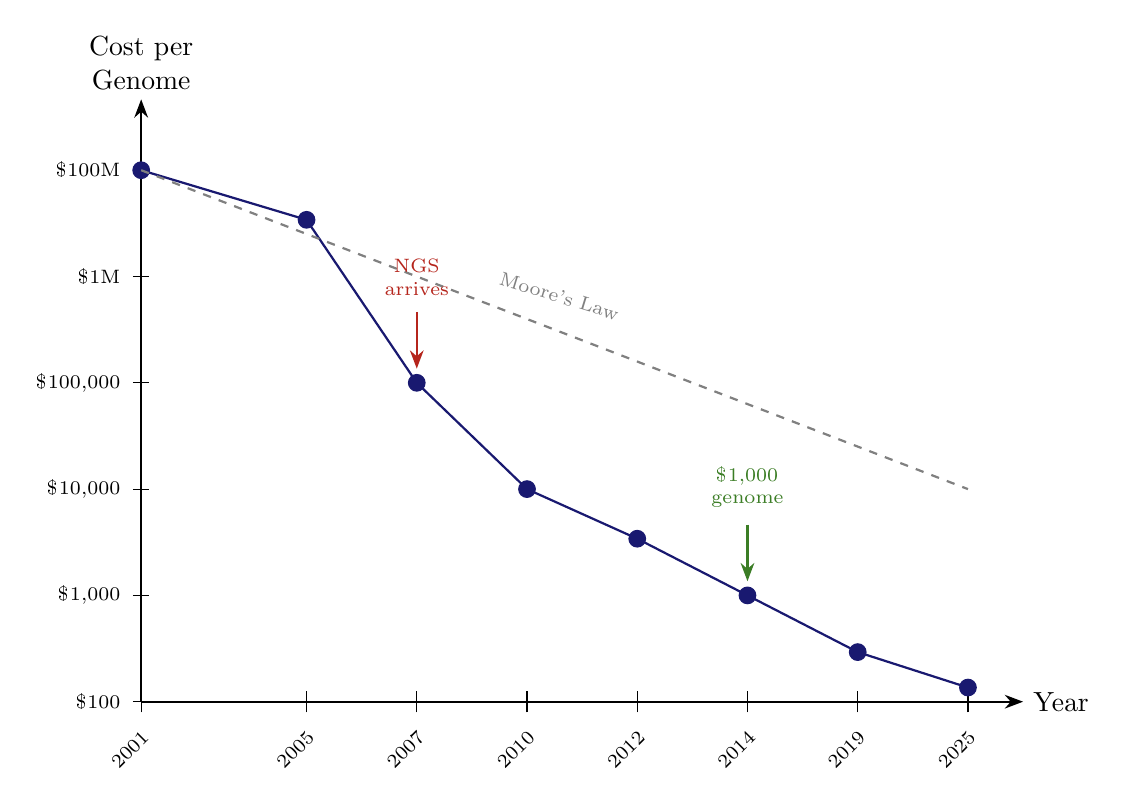
\begin{tikzpicture}[x=0.7cm, y=0.9cm]
  % Axes
  \draw[thick, -{Stealth}] (0,0) -- (16,0) node[right] {Year};
  \draw[thick, -{Stealth}] (0,0) -- (0,8.5) node[above, align=center] {Cost per\\Genome};

  % Y-axis labels (log scale conceptual)
  \foreach \y/\lab in {0/\$100, 1.5/\$1{,}000, 3/\$10{,}000, 4.5/\$100{,}000, 6/\$1M, 7.5/\$100M} {
    \draw (-0.15,\y) -- (0.15,\y);
    \node[left] at (-0.2,\y) {\scriptsize \lab};
  }

  % X-axis labels
  \foreach \x/\yr in {0/2001, 3/2005, 5/2007, 7/2010, 9/2012, 11/2014, 13/2019, 15/2025} {
    \draw (\x,-0.15) -- (\x,0.15);
    \node[below, rotate=45, anchor=north east] at (\x,-0.2) {\scriptsize \yr};
  }

  % Data points (approximate log-scale)
  \filldraw[MidnightBlue] (0,7.5) circle (3pt);   % 2001: ~$100M
  \filldraw[MidnightBlue] (3,6.8) circle (3pt);    % 2005: ~$50M
  \filldraw[MidnightBlue] (5,4.5) circle (3pt);    % 2007: $100K (NGS arrives)
  \filldraw[MidnightBlue] (7,3.0) circle (3pt);    % 2010: $10K
  \filldraw[MidnightBlue] (9,2.3) circle (3pt);    % 2012: ~$5K
  \filldraw[MidnightBlue] (11,1.5) circle (3pt);   % 2014: $1K
  \filldraw[MidnightBlue] (13,0.7) circle (3pt);   % 2019: ~$600
  \filldraw[MidnightBlue] (15,0.2) circle (3pt);   % 2025: ~$200

  % Line connecting points
  \draw[MidnightBlue, thick] (0,7.5) -- (3,6.8) -- (5,4.5) -- (7,3.0) -- (9,2.3) -- (11,1.5) -- (13,0.7) -- (15,0.2);

  % Moore's Law reference
  \draw[dashed, gray, thick] (0,7.5) -- (15,3.0);
  \node[gray, rotate=-17, anchor=south] at (7.5,5.5) {\scriptsize Moore's Law};

  % Annotation
  \draw[-{Stealth}, BrickRed, thick] (5,5.5) -- (5,4.7);
  \node[BrickRed, above, align=center, font=\scriptsize] at (5,5.6) {NGS\\arrives};

  \draw[-{Stealth}, OliveGreen, thick] (11,2.5) -- (11,1.7);
  \node[OliveGreen, above, align=center, font=\scriptsize] at (11,2.6) {\$1,000\\genome};
\end{tikzpicture}
\caption[Cost per human genome over time.]{The cost of sequencing a human genome has fallen faster than Moore's Law, particularly after the introduction of \acrshort{NGS} technologies around 2005--2007. Costs are approximate and reflect reagent costs.}
\label{fig:intro:cost-trajectory}
\end{figure}

This dramatic cost reduction---faster than Moore's Law for semiconductor performance (\cref{fig:intro:cost-trajectory})---has fundamentally democratised access to sequencing. What once required a billion-dollar international consortium can now be performed by a single graduate student with a desktop sequencer.

\begin{tipbox}
The cost of \textit{sequencing} a genome is only part of the total cost of a genomics project. Sample collection, DNA/RNA extraction, library preparation, computational infrastructure, data storage, and expert analysis can collectively exceed the sequencing cost itself. When budgeting for a project, consider the complete workflow.
\end{tipbox}


\section{The Different ``Omes''}
\label{sec:intro:omes}

Sequencing technologies do not just read DNA. Modern methods can interrogate many different layers of biological information. Each layer is described by its own ``-ome'' and the corresponding ``-omics'' field:

\subsection{The Genome}
\label{subsec:intro:genome}

The \textbf{genome} is the complete set of DNA in an organism. It includes all the genes (regions that encode proteins or functional RNAs) as well as vast stretches of non-coding DNA that play regulatory, structural, or still-unknown roles. \textbf{Genomics} is the study of genomes---their sequence, structure, function, and evolution. The human genome is approximately 3.2 billion base pairs long and is packaged into 23 pairs of chromosomes.

\subsection{The Transcriptome}
\label{subsec:intro:transcriptome}

The \textbf{transcriptome} is the complete set of RNA molecules in a cell or tissue at a given moment. While every cell in your body (with few exceptions) contains the same genome, different cell types express different subsets of genes. A liver cell transcribes a very different set of genes than a neuron. \textbf{Transcriptomics} captures this snapshot of gene expression, revealing which genes are ``on'' and at what level.

\subsection{The Epigenome}
\label{subsec:intro:epigenome}

The \textbf{epigenome} comprises the chemical modifications to DNA and its associated proteins (histones) that influence gene expression without changing the underlying DNA sequence. These modifications include \textbf{DNA methylation} (the addition of methyl groups to cytosine bases) and \textbf{histone modifications} (chemical tags on the protein spools around which DNA is wound). \textbf{Epigenomics} studies these modifications across the entire genome.

\subsection{The Proteome}
\label{subsec:intro:proteome}

The \textbf{proteome} is the complete set of proteins expressed by a cell, tissue, or organism. While the genome provides the blueprint and the transcriptome reflects which blueprints are being read, the proteome represents the actual molecular machines carrying out cellular functions. \textbf{Proteomics} traditionally uses mass spectrometry rather than sequencing, though sequencing-based methods (such as Ribo-seq for ribosome profiling) can provide indirect measurements of protein production.

\subsection{The Metabolome}
\label{subsec:intro:metabolome}

The \textbf{metabolome} is the complete set of small molecules (metabolites) present in a biological sample. These include sugars, lipids, amino acids, nucleotides, and the thousands of other small molecules involved in cellular metabolism. \textbf{Metabolomics} typically uses mass spectrometry or nuclear magnetic resonance (NMR), though it is sometimes integrated with sequencing-based multi-omics studies.

\subsection{The Microbiome}
\label{subsec:intro:microbiome}

The \textbf{microbiome} refers to the community of microorganisms---bacteria, archaea, fungi, viruses---that inhabit a particular environment, such as the human gut, soil, or ocean water. \textbf{Metagenomics} uses sequencing to identify and characterise these microbial communities, often without the need to culture individual species in the laboratory. This has revealed that the human body harbours trillions of microbial cells that play critical roles in health and disease.

\begin{keyconcept}[title={Multi-Omics}]
No single ``ome'' tells the complete story of a biological system. Modern research increasingly integrates data from multiple omics layers---genomics, transcriptomics, epigenomics, proteomics, and metabolomics---to build comprehensive models of cellular function and disease. Some cutting-edge single-cell technologies can even measure multiple omics layers simultaneously from the same individual cell.
\end{keyconcept}


\section{How Sequencing Has Transformed Science}
\label{sec:intro:transformations}

\subsection{Medicine and Clinical Diagnostics}
\label{subsec:intro:medicine}

Sequencing has fundamentally altered the practice of medicine in several ways:

\begin{itemize}[itemsep=3pt]
  \item \textbf{Cancer genomics:} Tumour sequencing identifies the specific mutations driving a patient's cancer, enabling \textbf{precision oncology}---the selection of targeted therapies matched to a tumour's molecular profile. Large-scale projects such as The Cancer Genome Atlas (TCGA) have catalogued mutations across dozens of cancer types.
  \item \textbf{Rare disease diagnosis:} For patients with undiagnosed genetic conditions, \acrfull{WGS} or \acrfull{WES} can identify the causal mutation. Studies have shown that genomic sequencing can provide a diagnosis for 25--40\% of previously undiagnosed rare disease patients.
  \item \textbf{Prenatal screening:} Non-invasive prenatal testing (NIPT) sequences cell-free fetal DNA circulating in the mother's blood to screen for chromosomal abnormalities such as Down syndrome (trisomy 21), with high sensitivity and specificity.
  \item \textbf{Pharmacogenomics:} Sequencing a patient's genome can reveal genetic variants that affect drug metabolism, helping clinicians choose the right drug and dosage.
  \item \textbf{Infectious disease:} Rapid sequencing of pathogen genomes enables real-time outbreak tracking, identification of antimicrobial resistance genes, and development of targeted diagnostics and vaccines. The COVID-19 pandemic demonstrated this on a global scale, with millions of SARS-CoV-2 genomes sequenced worldwide.
\end{itemize}

\subsection{Agriculture and Food Science}
\label{subsec:intro:agriculture}

Genomic sequencing has accelerated crop and livestock improvement. By sequencing the genomes of important crop species (rice, wheat, maize, soybean), researchers have identified genes associated with yield, drought tolerance, disease resistance, and nutritional quality. Genomic selection---using genome-wide genetic markers to predict an organism's traits---has dramatically shortened breeding cycles in both plants and animals.

\subsection{Ecology and Conservation Biology}
\label{subsec:intro:ecology}

Environmental DNA (eDNA) sequencing allows ecologists to survey biodiversity by collecting water or soil samples and sequencing the trace DNA shed by organisms. This non-invasive approach can detect rare or elusive species, monitor ecosystem health, and track the spread of invasive species. Population genomics studies use sequencing to assess genetic diversity within endangered species, informing conservation strategies.

\subsection{Forensic Science}
\label{subsec:intro:forensics}

DNA sequencing has become a cornerstone of forensic identification. Beyond traditional short tandem repeat (STR) profiling, \acrshort{NGS}-based forensic methods can extract more information from degraded or mixed samples, determine biogeographic ancestry, and even predict physical appearance traits from DNA.

\subsection{Evolutionary Biology and Palaeogenomics}
\label{subsec:intro:evolution}

Sequencing has illuminated the tree of life, resolving evolutionary relationships from viruses to vertebrates. Perhaps most spectacularly, advances in ancient DNA (aDNA) extraction and sequencing have enabled researchers to sequence genomes from organisms that died tens of thousands of years ago---including Neanderthals, Denisovans, woolly mammoths, and cave bears. Svante P\"a\"abo received the 2022 Nobel Prize in Physiology or Medicine for his pioneering work in palaeogenomics.


\section{What Modern Sequencing Can Measure}
\label{sec:intro:what-sequencing-measures}

The versatility of modern sequencing is remarkable. By varying the sample preparation (called \textbf{library preparation}---see \cref{ch:seqprinciples}), the same sequencing instrument can be used to measure fundamentally different biological properties:

\begin{table}[htbp]
\centering
\caption[Biological layers measurable by sequencing.]{Major biological layers that can be interrogated using sequencing-based approaches.}
\label{tab:intro:measurement-types}
\small
\begin{tabularx}{\textwidth}{>{\bfseries}l X l}
\toprule
\textbf{What Is Measured} & \textbf{Description} & \textbf{Key Methods} \\
\midrule
DNA sequence & The order of bases in the genome & \acrshort{WGS}, \acrshort{WES} \\
\addlinespace
RNA expression & Which genes are active and at what level & \acrshort{RNA-seq}, \acrshort{scRNA-seq} \\
\addlinespace
DNA methylation & Methyl groups on cytosine residues & \acrshort{WGBS}, RRBS, nanopore \\
\addlinespace
Chromatin accessibility & Which genomic regions are ``open'' and potentially active & \acrshort{ATAC-seq}, DNase-seq \\
\addlinespace
Protein--DNA interactions & Where proteins bind to the genome & \acrshort{ChIP-seq}, CUT\&RUN \\
\addlinespace
Spatial gene expression & Gene expression mapped to tissue location & 10x Visium, MERFISH, Slide-seq \\
\addlinespace
3D genome architecture & How the genome folds in three-dimensional space & \acrshort{Hi-C}, Micro-C, GAM \\
\addlinespace
Microbial communities & Species composition of complex microbial ecosystems & 16S/ITS amplicon, shotgun metagenomics \\
\bottomrule
\end{tabularx}
\end{table}

As shown in \cref{tab:intro:measurement-types}, the key insight is that \textit{the sequencing instrument itself is largely agnostic to what is being measured}. The specificity comes from how the sample is prepared before sequencing. This concept---that library preparation defines the experiment---is one of the most important ideas in modern genomics and will be explored in detail throughout this book.

\begin{warningbox}
Sequencing measures \textbf{nucleic acid sequences}. It does not directly measure protein levels, metabolite concentrations, or protein structures. When we say ``sequencing measures chromatin accessibility'' or ``protein--DNA interactions,'' we mean that a clever biochemical protocol converts these properties into a DNA sequencing readout. Understanding these conversions is essential for interpreting sequencing data correctly.
\end{warningbox}


\section{The General Sequencing Workflow}
\label{sec:intro:general-workflow}

Although each sequencing application has its own specific protocol, all sequencing experiments share a common high-level workflow. Understanding this workflow provides a conceptual framework for the rest of the book.

\begin{figure}[htbp]
\centering
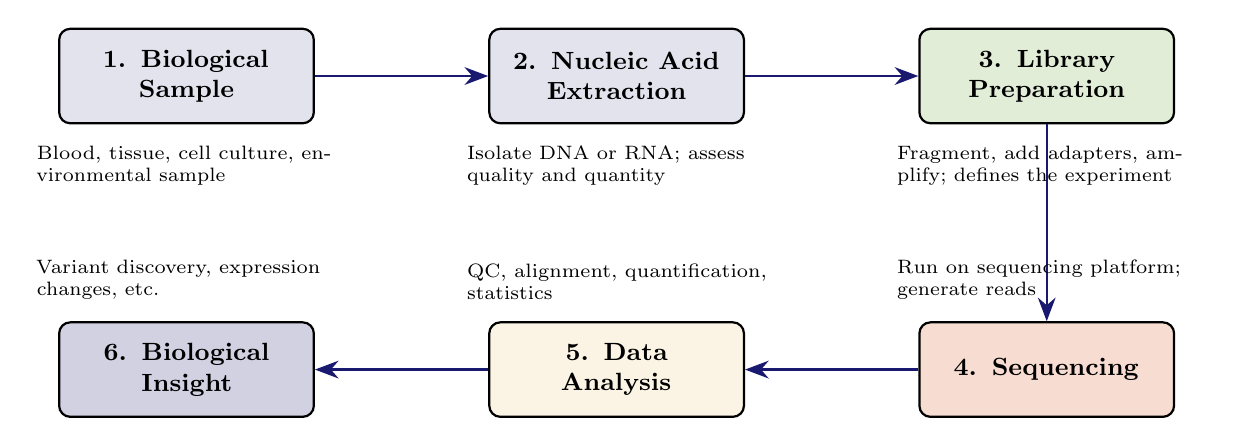
\begin{tikzpicture}[
  node distance=1.5cm,
  box/.style={
    draw, rounded corners=4pt, thick,
    minimum width=3.2cm, minimum height=1.2cm,
    text width=3cm, align=center, font=\small\bfseries
  },
  arrow/.style={-{Stealth[length=3mm]}, thick, MidnightBlue},
  desc/.style={font=\scriptsize, text width=3.8cm, align=left}
]

% Boxes
\node[box, fill=MidnightBlue!12] (sample) {1. Biological\\Sample};
\node[box, fill=MidnightBlue!12, right=2.2cm of sample] (extract) {2. Nucleic Acid\\Extraction};
\node[box, fill=OliveGreen!12, right=2.2cm of extract] (library) {3. Library\\Preparation};
\node[box, fill=BrickRed!12, below=2.5cm of library] (sequencing) {4. Sequencing};
\node[box, fill=Goldenrod!12, left=2.2cm of sequencing] (analysis) {5. Data\\Analysis};
\node[box, fill=MidnightBlue!20, left=2.2cm of analysis] (insight) {6. Biological\\Insight};

% Arrows
\draw[arrow] (sample) -- (extract);
\draw[arrow] (extract) -- (library);
\draw[arrow] (library) -- (sequencing);
\draw[arrow] (sequencing) -- (analysis);
\draw[arrow] (analysis) -- (insight);

% Descriptions
\node[desc, below=0.15cm of sample] {Blood, tissue, cell culture, environmental sample};
\node[desc, below=0.15cm of extract] {Isolate DNA or RNA; assess quality and quantity};
\node[desc, below=0.15cm of library] {Fragment, add adapters, amplify; defines the experiment};
\node[desc, above=0.15cm of sequencing] {Run on sequencing platform; generate reads};
\node[desc, above=0.15cm of analysis] {QC, alignment, quantification, statistics};
\node[desc, above=0.15cm of insight] {Variant discovery, expression changes, etc.};

\end{tikzpicture}
\caption[The general sequencing workflow.]{The general sequencing workflow, from biological sample to biological insight. Every sequencing experiment follows some version of this pipeline.}
\label{fig:intro:general-workflow}
\end{figure}

\subsection{Step 1: Biological Sample}
\label{subsec:intro:sample}

Every sequencing experiment begins with a biological sample. This could be blood drawn from a patient, a tissue biopsy, a bacterial culture, a water sample from a lake, soil, or even ancient bone. The nature and quality of the starting material profoundly influence every downstream step. A fresh, well-preserved sample will yield high-quality nucleic acids; a degraded or contaminated sample may produce unreliable results.

\subsection{Step 2: Nucleic Acid Extraction}
\label{subsec:intro:extraction}

The DNA or RNA must be isolated from the sample. Extraction protocols use chemical and physical methods to break open cells (lysis), remove proteins and other contaminants, and purify the nucleic acids. The quality and quantity of extracted material are assessed using instruments such as a spectrophotometer (e.g., NanoDrop), a fluorometer (e.g., Qubit), or electrophoresis (e.g., Bioanalyzer, TapeStation).

\subsection{Step 3: Library Preparation}
\label{subsec:intro:library-prep}

This is the step where the nucleic acid is converted into a form compatible with the sequencing instrument. The details vary enormously depending on the application, but the general steps include:

\begin{enumerate}[itemsep=2pt]
  \item \textbf{Fragmentation:} Breaking the nucleic acid into pieces of an appropriate size (e.g., 200--500\basepair{} for short-read sequencing).
  \item \textbf{Adapter ligation:} Attaching short, synthetic DNA sequences (adapters) to the ends of fragments. These adapters allow fragments to bind to the sequencing instrument and serve as priming sites for sequencing.
  \item \textbf{Amplification:} Using \acrfull{PCR} to create multiple copies of each library fragment (though some protocols are ``PCR-free'').
  \item \textbf{Selection or enrichment:} Optionally selecting fragments of a specific size or enriching for specific genomic regions (e.g., exome capture).
\end{enumerate}

The resulting collection of adapter-ligated fragments is called a \textbf{sequencing library}. This concept is explored in depth in \cref{ch:seqprinciples}.

\subsection{Step 4: Sequencing}
\label{subsec:intro:sequencing}

The library is loaded onto a sequencing instrument, which reads the sequence of each fragment. Different platforms use different chemistries (discussed in \cref{ch:seqprinciples} and subsequent chapters), but all produce the same fundamental output: millions to billions of short text strings representing the sequences of the library fragments, along with quality scores indicating the confidence of each base call.

\subsection{Step 5: Data Analysis}
\label{subsec:intro:analysis}

The raw sequencing data (typically in \acrshort{FASTQ} format) must be processed computationally. A typical analysis pipeline involves:

\begin{enumerate}[itemsep=2pt]
  \item \textbf{Quality control:} Assessing data quality and removing low-quality reads or adapter sequences.
  \item \textbf{Alignment / Mapping:} Aligning reads to a reference genome to determine where each read originated.
  \item \textbf{Quantification or variant calling:} Counting reads per gene (for expression analysis) or identifying positions where the sample differs from the reference (for variant calling).
  \item \textbf{Statistical analysis:} Applying statistical methods to identify significant biological signals (e.g., differentially expressed genes, significantly mutated regions).
  \item \textbf{Visualisation and interpretation:} Presenting results in an interpretable format and placing them in biological context.
\end{enumerate}

\subsection{Step 6: Biological Insight}
\label{subsec:intro:insight}

The ultimate goal of any sequencing experiment is biological understanding. This might be identifying the mutation causing a patient's disease, discovering a new gene regulatory mechanism, characterising the microbial community in a specific environment, or any of thousands of other scientific questions that sequencing can address.

\begin{tipbox}
A common mistake for beginners is to focus exclusively on the sequencing step itself, underestimating the importance of sample quality, library preparation, and computational analysis. In practice, the ``wetlab'' steps (sample prep and library construction) and the ``drylab'' steps (bioinformatics and statistics) are at least as important as the sequencing itself. Garbage in, garbage out.
\end{tipbox}


\section{The Cost Trajectory and Democratisation of Sequencing}
\label{sec:intro:cost}

The cost of sequencing has decreased at a pace that outstrips even the famous Moore's Law for computer transistors. As illustrated in \cref{fig:intro:cost-trajectory}, the cost of sequencing a human genome fell from approximately \$100 million in 2001 to under \$200 by 2025---a decline of roughly six orders of magnitude in 24 years.

This cost reduction has had profound consequences:

\begin{itemize}[itemsep=3pt]
  \item \textbf{Democratisation:} Sequencing is no longer restricted to a handful of large genome centres. University core facilities, clinical laboratories, and even field stations now operate sequencing instruments. The Oxford Nanopore MinION, which costs roughly \$1,000 and is the size of a stapler, has been used in Antarctic research stations, the International Space Station, and disease outbreak zones in remote regions of Africa.

  \item \textbf{Scale:} Projects like the UK Biobank (500,000 genomes), the All of Us Research Program (1 million+ participants), and large-scale cancer genomics initiatives would have been unthinkable at earlier cost points.

  \item \textbf{Clinical adoption:} As costs have fallen, sequencing has moved from a research tool to a clinical diagnostic. Many hospitals now offer clinical \acrshort{WGS} or \acrshort{WES} for rare disease diagnosis, and tumour sequencing panels are standard of care in oncology.

  \item \textbf{New applications:} Low costs have enabled entirely new categories of experiments, such as single-cell sequencing (profiling thousands to millions of individual cells), spatial transcriptomics (mapping gene expression to tissue locations), and real-time pathogen surveillance.
\end{itemize}

\begin{warningbox}
While sequencing costs have plummeted, the costs of data storage, computational analysis, and expert interpretation have not decreased at the same rate. For large-scale projects generating petabytes of data, computational costs can exceed sequencing costs. This growing imbalance is sometimes called the ``\$1,000 genome, \$1,000,000 analysis'' problem.
\end{warningbox}


\section{The Current Sequencing Landscape}
\label{sec:intro:landscape}

As of the mid-2020s, the sequencing landscape is dominated by a few major technology families:

\begin{description}[style=nextline, itemsep=4pt]
  \item[Short-read sequencing (Illumina)] The most widely used platform, producing reads of 50--300\basepair{} with very high accuracy (>99.9\% per base). Dominant for applications requiring high throughput: \acrshort{WGS}, \acrshort{RNA-seq}, \acrshort{ChIP-seq}, \acrshort{ATAC-seq}, and most clinical diagnostics.

  \item[Long-read sequencing (PacBio SMRT)] Produces reads averaging 15--25\kilobase{} (and up to >100\kilobase{}), with high consensus accuracy achieved through circular consensus sequencing (HiFi reads). Excellent for genome assembly, structural variant detection, and full-length transcript sequencing.

  \item[Long-read sequencing (Oxford Nanopore)] Produces ultra-long reads (routinely >100\kilobase{}, with records exceeding 4\megabase{}). Can directly detect base modifications (e.g., methylation) without chemical conversion. Uniquely portable (MinION) and capable of real-time data streaming.

  \item[Emerging platforms] New entrants, including Element Biosciences (AVITI), Ultima Genomics, and others, are introducing competition in the short-read space with novel chemistries and pricing models.
\end{description}

These platforms are covered in detail in \cref{ch:seqprinciples} and the chapters that follow.


% ============================================================
\section{An Information-Theoretic View of Sequencing}
\label{sec:intro:information-theory}

Sequencing can be framed as an information-recovery problem. A genome of length $G$ bases, drawn from an alphabet of size $|\Sigma|=4$, carries at most $2G$ bits of information (since $\log_2 4 = 2$). In practice, the information content is lower because of compositional biases. The \textbf{Shannon entropy} of a sequence quantifies this:

\begin{equation}
H = -\sum_{i \in \{A,C,G,T\}} p_i \log_2 p_i
\label{eq:intro:shannon-entropy}
\end{equation}

where $p_i$ is the frequency of base $i$. For a genome with perfectly uniform composition ($p_A = p_C = p_G = p_T = 0.25$), $H = 2$ bits per position. For an AT-rich genome such as \species{Plasmodium falciparum} ($\sim$80\% AT), $H \approx 1.72$ bits per position, meaning the sequence is intrinsically more compressible and, in a sense, carries less information per base.

\begin{keyconcept}[title={Shannon Entropy and Genome Complexity}]
Shannon entropy provides a rigorous lower bound on the number of bits needed to encode each position in a genome. This quantity has direct practical consequences: genomes with low entropy (e.g., highly repetitive or AT-biased) are easier to compress (relevant for storage), but harder to assemble (because repeats create ambiguity in fragment overlap). Entropy also constrains the theoretical minimum number of reads required to reconstruct a genome, a result formalised by information-theoretic limits on sequence assembly.
\end{keyconcept}

This perspective connects to a practical trade-off: every sequencing experiment must generate enough information (reads $\times$ read length $\times$ accuracy) to overcome the entropy of the target plus the noise introduced by the instrument's error rate. For a base call with error probability $P_e$, the mutual information between the true base and the observed call is:

\begin{equation}
I = \log_2 |\Sigma| + P_e \log_2 \frac{P_e}{|\Sigma|-1} + (1-P_e)\log_2(1-P_e)
\label{eq:intro:mutual-info}
\end{equation}

At Q30 accuracy ($P_e = 0.001$), each observed base carries $\sim$1.99 bits of information---nearly all of the 2-bit theoretical maximum. At Q10 ($P_e = 0.1$), this drops to $\sim$1.53 bits, meaning roughly 30\% more sequencing is needed to achieve the same total information content.


\subsection{Quantitative Comparison of Sequencing Generations}
\label{subsec:intro:generation-comparison}

The evolution of sequencing technology can be summarised quantitatively across several dimensions. \Cref{tab:intro:generation-comparison} provides a comprehensive comparison.

\begin{table}[htbp]
\centering
\caption[Quantitative comparison of sequencing generations.]{Quantitative comparison of sequencing technology generations. Costs are approximate and reflect the mid-2020s.}
\label{tab:intro:generation-comparison}
\small
\begin{tabularx}{\textwidth}{>{\bfseries}l X X X X}
\toprule
\textbf{Metric} & \textbf{Sanger} & \textbf{2nd Gen (Illumina)} & \textbf{3rd Gen (PacBio HiFi)} & \textbf{3rd Gen (ONT)} \\
\midrule
Read length & 500--1,000\basepair{} & 50--300\basepair{} & 10--25\kilobase{} & 1\kilobase{}--4\megabase{} \\
\addlinespace
Per-read accuracy & 99.99\% & 99.9\% (Q30) & 99.9\% (Q30 HiFi) & 92--99\% (raw) \\
\addlinespace
Throughput / run & $\sim$0.1\megabase{} & 0.6--16,000\gigabase{} & 15--90\gigabase{} & 2--300\gigabase{} \\
\addlinespace
Reads / run & 96 & $10^6$--$10^{10}$ & $10^5$--$10^7$ & $10^4$--$10^7$ \\
\addlinespace
Cost / Gb & \$500,000 & \$2--20 & \$20--50 & \$5--30 \\
\addlinespace
Instrument cost & \$90K & \$20K--1.0M & \$200K--600K & \$1K--48K \\
\addlinespace
Time to result & 2--3 h & 12--48 h & 12--30 h & 1 h--72 h \\
\addlinespace
Dominant error & Substitution & Substitution & Indel (residual) & Indel (homopolymer) \\
\addlinespace
Base modifications & No & No (indirect only) & Yes (kinetics) & Yes (direct signal) \\
\bottomrule
\end{tabularx}
\end{table}

\begin{figure}[htbp]
\centering
\begin{tikzpicture}[
  bubble/.style={circle, draw=#1, thick, fill=#1!15, inner sep=0pt, font=\scriptsize\bfseries, align=center},
]
  % Axes
  \draw[thick, -{Stealth[length=3mm]}] (0,0) -- (13,0) node[right] {\small Read length};
  \draw[thick, -{Stealth[length=3mm]}] (0,0) -- (0,8) node[above] {\small Throughput};

  % Axis labels
  \node[below, font=\scriptsize] at (1,-0.3) {100\basepair{}};
  \node[below, font=\scriptsize] at (4,-0.3) {1\kilobase{}};
  \node[below, font=\scriptsize] at (7.5,-0.3) {10\kilobase{}};
  \node[below, font=\scriptsize] at (11,-0.3) {100\kilobase{}+};

  \node[left, font=\scriptsize] at (-0.2,1.5) {Low};
  \node[left, font=\scriptsize] at (-0.2,4) {Med};
  \node[left, font=\scriptsize] at (-0.2,6.5) {High};

  % Sanger bubble (small, short reads, low throughput)
  \node[bubble=gray, minimum size=0.8cm] at (1.5,0.8) {Sanger};

  % Illumina bubble (large for throughput, short reads)
  \node[bubble=MidnightBlue, minimum size=2.2cm] at (2.5,6.5) {Illumina};

  % PacBio HiFi (medium throughput, long reads)
  \node[bubble=OliveGreen, minimum size=1.6cm] at (7.5,4.0) {PacBio\\HiFi};

  % ONT (medium throughput, ultra-long reads possible)
  \node[bubble=BrickRed, minimum size=1.4cm] at (10.5,3.5) {ONT};

  % Annotation: bubble size = cost-effectiveness
  \node[font=\scriptsize\itshape, text width=3cm, align=center] at (11,7) {Bubble size $\propto$\\cost-effectiveness\\(Gb per \$)};
\end{tikzpicture}
\caption[Sequencing platform comparison.]{Conceptual comparison of major sequencing platforms. The $x$-axis represents read length, the $y$-axis represents throughput per run, and bubble size approximates cost-effectiveness. Each technology occupies a distinct niche; the choice depends on the biological question.}
\label{fig:intro:platform-bubbles}
\end{figure}

The key insight from this comparison is that \textit{no single platform dominates across all dimensions}. Short-read platforms excel in throughput and cost per base, making them ideal for large-scale surveys (population genomics, RNA-seq). Long-read platforms sacrifice some throughput for the ability to resolve complex genomic features (structural variants, repeat-rich regions, full-length transcripts, base modifications). This complementarity is why many modern studies employ a hybrid approach, combining short and long reads to leverage the strengths of both.


% ============================================================
\section{Reading Guide for This Book}
\label{sec:intro:reading-guide}

This book is organised into seven parts, designed to take you from foundational concepts to advanced applications and analysis:

\begin{description}[style=nextline, itemsep=4pt]
  \item[Part~I: Foundations (Chapters~\ref{ch:introduction}--\ref{ch:seqprinciples})]
  You are here. \Cref{ch:molbio} covers the essential molecular biology you need to understand sequencing technologies---DNA structure, gene expression, epigenetics, and genetic variation. \Cref{ch:seqprinciples} introduces the core principles shared by all modern sequencing platforms: how reads are generated, what quality scores mean, and key concepts like coverage and multiplexing.

  \item[Part~II: Sequencing Platforms and Technologies (Chapters~4--6)]
  A detailed survey of current sequencing instruments. Chapter~4 covers short-read platforms (Illumina and emerging competitors). Chapter~5 covers long-read platforms (PacBio and Oxford Nanopore). Chapter~6 provides a comprehensive guide to library preparation methods.

  \item[Part~III: Genomics (Chapters~7--9)]
  DNA-level applications: whole-genome sequencing, exome sequencing, variant discovery and annotation, and metagenomics for microbial community analysis.

  \item[Part~IV: Transcriptomics (Chapters~10--12)]
  RNA-level applications: bulk \acrshort{RNA-seq}, single-cell \acrshort{RNA-seq} (\acrshort{scRNA-seq}), and spatial transcriptomics. These chapters cover both experimental design and computational analysis.

  \item[Part~V: Epigenomics (Chapters~13--16)]
  Epigenomic applications: DNA methylation profiling (\acrshort{WGBS} and related methods), chromatin accessibility (\acrshort{ATAC-seq}, DNase-seq), histone modification mapping (\acrshort{ChIP-seq}, CUT\&RUN/CUT\&Tag), and three-dimensional genome architecture (\acrshort{Hi-C}).

  \item[Part~VI: Multiomics and Emerging Frontiers (Chapters~17--19)]
  Cutting-edge technologies that measure multiple molecular layers simultaneously, specialised applications (long-read transcriptomics, direct RNA sequencing, spatial multi-omics), and emerging technologies poised to reshape the field.

  \item[Part~VII: Bioinformatics and Data Analysis (Chapters~20--23)]
  Computational fundamentals: file formats, alignment algorithms, workflow management (Nextflow, Snakemake), experimental design and statistical considerations, data standards, and reproducibility.

  \item[Part~VIII: Democratisation of Sequencing (Chapters~24--26)]
  Hands-on genomics for everyone. \Cref{ch:accessible} surveys accessible sequencing platforms and cost models for individual researchers and citizen scientists. \Cref{ch:protocols} provides step-by-step wet-lab protocols---from DNA extraction through library preparation to flow cell loading. \Cref{ch:diyanalysis} walks you through complete computational analyses, from basecalling to genome assembly and species identification, with full Snakemake and Nextflow workflows.
\end{description}

\begin{tipbox}[title={How to Use This Book}]
If you are completely new to genomics, we recommend reading Part~I (Chapters~\ref{ch:introduction}--\ref{ch:seqprinciples}) in full before branching into the topics most relevant to your work. If you already have a molecular biology background, you can skim \cref{ch:molbio} and start with \cref{ch:seqprinciples}. Each application chapter (Parts~III--VI) is designed to be relatively self-contained, so you can jump directly to the application most relevant to your research.
\end{tipbox}


\section{Summary}
\label{sec:intro:summary}

This chapter has provided a bird's-eye view of the sequencing revolution:

\begin{itemize}[itemsep=2pt]
  \item Sequencing is the process of reading the nucleotide sequence of DNA or RNA, and it has become one of the most transformative technologies in modern science.
  \item From Sanger sequencing in 1977 through the Human Genome Project and the \acrshort{NGS} revolution, the cost and speed of sequencing have improved by many orders of magnitude.
  \item Modern sequencing can interrogate many biological layers beyond DNA sequence, including gene expression, epigenetic modifications, chromatin structure, protein--DNA interactions, and spatial gene expression patterns.
  \item The general workflow---sample collection, nucleic acid extraction, library preparation, sequencing, data analysis, and biological interpretation---provides a framework for understanding all sequencing experiments.
  \item The dramatic decrease in sequencing costs has democratised the technology, enabling applications from clinical diagnostics to ecological surveys to palaeogenomics.
\end{itemize}

In the next chapter, we will build the molecular biology foundation you need to understand how these technologies work at the chemical and biological level.

\chapter{Molecular Biology Essentials}
\label{ch:molbio}

\begin{keyconcept}
Before we can understand how sequencing technologies work, we need to understand what they are reading. This chapter builds the molecular biology foundation---from the structure of cells and DNA to gene expression, epigenetics, and genetic variation---that underpins every sequencing experiment described in this book. If you already have a strong background in molecular biology, you may wish to skim this chapter and use it as a reference.
\end{keyconcept}

% ============================================================
\section{The Cell: Life's Fundamental Unit}
\label{sec:molbio:cell}

All living organisms are composed of cells. A cell is the smallest unit of life capable of independent function: it can take in nutrients, produce energy, grow, and reproduce. There are two fundamentally different types of cells, distinguished by their internal organisation.

\subsection{Prokaryotic Cells}
\label{subsec:molbio:prokaryotes}

\textbf{Prokaryotes}---bacteria and archaea---are the simplest and most ancient cells. A prokaryotic cell lacks a membrane-bound nucleus; instead, its DNA floats freely in the cytoplasm in a region called the \textbf{nucleoid}. Key features include:

\begin{itemize}[itemsep=2pt]
  \item \textbf{No nucleus:} DNA is not enclosed in a membrane-bound compartment.
  \item \textbf{Circular chromosome:} Most prokaryotic genomes consist of a single, circular DNA molecule (though some prokaryotes have linear chromosomes or multiple chromosomes).
  \item \textbf{Small genomes:} Typically 0.5--10 million base pairs (\megabase{}), encoding 500--10,000 genes.
  \item \textbf{Plasmids:} Many prokaryotes carry small, circular, extra-chromosomal DNA molecules called plasmids, which often carry genes for antibiotic resistance or other survival advantages.
  \item \textbf{No membrane-bound organelles:} Prokaryotes lack the internal compartmentalisation seen in eukaryotic cells.
  \item \textbf{Operons:} Prokaryotic genes are often organised into \textbf{operons}---clusters of genes transcribed together as a single unit, under the control of a shared promoter.
\end{itemize}

\subsection{Eukaryotic Cells}
\label{subsec:molbio:eukaryotes}

\textbf{Eukaryotes}---animals, plants, fungi, and protists---have larger, more complex cells with a \textbf{membrane-bound nucleus} that houses the DNA. Key features include:

\begin{itemize}[itemsep=2pt]
  \item \textbf{Nucleus:} The DNA is enclosed within a double membrane called the \textbf{nuclear envelope}, which separates the genetic material from the cytoplasm.
  \item \textbf{Linear chromosomes:} Eukaryotic genomes are organised into multiple linear chromosomes. Humans have 23 pairs (46 total).
  \item \textbf{Large genomes:} Ranging from about 10\megabase{} (some fungi) to over 100\gigabase{} (some plants and amphibians). The human genome is approximately 3.2\gigabase{}.
  \item \textbf{Membrane-bound organelles:} Including \textbf{mitochondria} (energy production, with their own small circular genome), \textbf{endoplasmic reticulum} (protein and lipid synthesis), \textbf{Golgi apparatus} (protein sorting and modification), and in plants, \textbf{chloroplasts} (photosynthesis, also with their own genome).
  \item \textbf{Complex gene structure:} Eukaryotic genes are typically split into coding segments (\textbf{exons}) interrupted by non-coding segments (\textbf{introns}), and each gene usually has its own promoter.
\end{itemize}

\begin{tipbox}
When sequencing eukaryotic organisms, remember that the cell contains DNA in multiple locations: the nuclear genome (the main focus of most sequencing experiments), the mitochondrial genome, and in plants, the chloroplast genome. Reads from these organellar genomes will appear in your data and must be accounted for during analysis.
\end{tipbox}


% ============================================================
\section{DNA Structure: The Molecule of Heredity}
\label{sec:molbio:dna-structure}

Deoxyribonucleic acid (\textbf{DNA}) is the molecule that stores genetic information in all cellular organisms (and many viruses). Understanding its structure is essential for understanding how sequencing works.

\subsection{Nucleotides: The Building Blocks}
\label{subsec:molbio:nucleotides}

DNA is a \textbf{polymer}---a long chain made up of repeating subunits called \textbf{nucleotides}. Each nucleotide consists of three components:

\begin{enumerate}[itemsep=2pt]
  \item \textbf{A sugar:} Deoxyribose, a five-carbon sugar. The carbon atoms are numbered 1$'${} through 5$'${} (pronounced ``one prime'' through ``five prime'').
  \item \textbf{A phosphate group:} Attached to the 5$'${} carbon of the sugar.
  \item \textbf{A nitrogenous base:} One of four molecules that project inward from the sugar-phosphate backbone:
  \begin{itemize}
    \item \textbf{Adenine (A)} --- a purine (two-ring structure)
    \item \textbf{Guanine (G)} --- a purine (two-ring structure)
    \item \textbf{Cytosine (C)} --- a pyrimidine (single-ring structure)
    \item \textbf{Thymine (T)} --- a pyrimidine (single-ring structure)
  \end{itemize}
\end{enumerate}

Nucleotides are linked together by \textbf{phosphodiester bonds} between the 3$'${} carbon of one nucleotide and the 5$'${} carbon of the next, forming a continuous \textbf{sugar-phosphate backbone}. The sequence of bases along this backbone encodes genetic information---much like the sequence of letters in a sentence encodes meaning.

\subsection{The Double Helix}
\label{subsec:molbio:double-helix}

In 1953, James Watson and Francis Crick---building on X-ray crystallography data from Rosalind Franklin and Maurice Wilkins---proposed that DNA has a \textbf{double-helical} structure: two strands of nucleotides wound around each other in a right-handed helix.

The two strands are held together by \textbf{hydrogen bonds} between complementary bases:
\begin{itemize}[itemsep=2pt]
  \item \textbf{A pairs with T} (via two hydrogen bonds)
  \item \textbf{G pairs with C} (via three hydrogen bonds)
\end{itemize}

This \textbf{base-pairing rule} (also called \textbf{Chargaff's rule}) is fundamental to both the biology of DNA and the chemistry of sequencing. Because G-C base pairs have three hydrogen bonds (compared to two for A-T), regions of DNA with high G-C content are more thermally stable and require more energy to separate (``melt'')---a property with important consequences for sequencing, as discussed in \cref{ch:seqprinciples}.

\subsection{Nucleotide Chemistry in Detail}
\label{subsec:molbio:nucleotide-chemistry}

The behaviour of nucleotides during sequencing depends critically on their chemical properties. Each nucleotide is a weak polyprotic acid whose ionisation state varies with pH:

\begin{table}[htbp]
\centering
\caption[Nucleobase pKa values and tautomeric equilibria.]{pKa values for the major ionisable groups of the four DNA bases. The dominant tautomeric form at physiological pH (7.4) is the \textbf{keto/amino} form, but rare tautomers can cause misincorporation during replication and sequencing.}
\label{tab:molbio:pka}
\small
\begin{tabular}{llcc}
\toprule
\textbf{Base} & \textbf{Ionisable group} & \textbf{pKa} & \textbf{Rare tautomer} \\
\midrule
Adenine & N-1 (protonation) & 3.5 & Imino form \\
Guanine & N-7 (protonation) & 3.3 & Enol form \\
        & N-1 (deprotonation) & 9.2 & \\
Cytosine & N-3 (protonation) & 4.5 & Imino form \\
Thymine  & N-3 (deprotonation) & 9.9 & Enol form \\
\bottomrule
\end{tabular}
\end{table}

\textbf{Tautomeric forms} of nucleobases---rare structural isomers in which a proton shifts between nitrogen and oxygen atoms---are of particular significance. When a base transiently adopts its rare tautomer, it can form non-canonical base pairs (e.g., enol-T pairs with G instead of A, imino-C pairs with A instead of G). This is one of the fundamental mechanisms of spontaneous mutation during DNA replication, with tautomeric mispairing occurring at rates of approximately $10^{-4}$ to $10^{-5}$ per base pair.

\begin{warningbox}[title={Tautomers and Sequencing Errors}]
The same tautomeric equilibria that cause natural replication errors can also affect sequencing accuracy. In sequencing-by-synthesis, a rare tautomer of the template base may cause the polymerase to incorporate the wrong fluorescent nucleotide. This contributes to the small but non-zero substitution error rate observed even in high-fidelity platforms such as Illumina.
\end{warningbox}


\subsection{DNA Thermodynamics and the Nearest-Neighbour Model}
\label{subsec:molbio:thermodynamics}

The thermal stability of DNA---its resistance to strand separation (``melting'')---is central to many molecular biology and sequencing techniques, including \acrshort{PCR}, hybridisation-based capture, and adapter ligation. The \textbf{melting temperature} ($T_m$) is defined as the temperature at which 50\% of DNA molecules in solution are in the double-stranded state and 50\% are single-stranded.

The most accurate method for predicting $T_m$ is the \textbf{nearest-neighbour (NN) model}, which accounts for the fact that the stability of a base pair depends not only on the pair itself but also on its neighbours (stacking interactions):

\begin{equation}
T_m = \frac{\Delta H^\circ}{\Delta S^\circ + R \ln(C_T/4)} - 273.15
\label{eq:molbio:tm-nn}
\end{equation}

where $\Delta H^\circ$ and $\Delta S^\circ$ are the total enthalpy and entropy of duplex formation (summed over all nearest-neighbour pairs), $R = 1.987$ cal/(mol$\cdot$K) is the gas constant, and $C_T$ is the total strand concentration. The thermodynamic parameters are calculated as:

\begin{align}
\Delta H^\circ &= \sum_{i=1}^{n-1} \Delta H^\circ_i + \Delta H^\circ_{\text{init}} \label{eq:molbio:dh-nn} \\
\Delta S^\circ &= \sum_{i=1}^{n-1} \Delta S^\circ_i + \Delta S^\circ_{\text{init}} + \Delta S^\circ_{\text{sym}} \label{eq:molbio:ds-nn}
\end{align}

where $\Delta H^\circ_i$ and $\Delta S^\circ_i$ are the enthalpy and entropy contributions of the $i$th nearest-neighbour pair, $\Delta H^\circ_{\text{init}}$ and $\Delta S^\circ_{\text{init}}$ are initiation parameters (dependent on the terminal base pairs), and $\Delta S^\circ_{\text{sym}} = -1.4$ cal/(mol$\cdot$K) is a symmetry correction applied to self-complementary sequences.

\begin{keyconcept}[title={Nearest-Neighbour Parameters}]
The 10 unique nearest-neighbour pairs (e.g., AA/TT, AT/TA, TA/AT, CA/GT, GT/CA, CT/GA, GA/CT, CG/GC, GC/CG, GG/CC) each have experimentally determined $\Delta H^\circ$ and $\Delta S^\circ$ values. For example, the GC/CG pair ($\Delta H^\circ = -9.8$ kcal/mol) is substantially more stable than the AA/TT pair ($\Delta H^\circ = -7.9$ kcal/mol). These parameters are used by primer design tools such as \software{Primer3} and \software{OligoAnalyzer} to predict hybridisation behaviour.
\end{keyconcept}

For practical estimation of short oligonucleotides (primers, adapters) in standard PCR buffer, a salt-adjusted approximation is often used:

\begin{equation}
T_m \approx T_m^{1\text{M NaCl}} + 16.6 \cdot \log_{10}[\text{Na}^+]
\label{eq:molbio:tm-salt}
\end{equation}

\begin{tipbox}
When designing sequencing adapters or \acrshort{PCR} primers, ensure that the $T_m$ of all oligos is within 1--2$\,^\circ$C of each other to promote uniform hybridisation and extension. Online tools such as \software{Primer3}, \software{IDT OligoAnalyzer}, and \software{NEB Tm Calculator} implement the full nearest-neighbour model with salt corrections and are freely available.
\end{tipbox}


\subsection{Directionality and Antiparallel Strands}
\label{subsec:molbio:directionality}

Each strand of DNA has a \textbf{directionality}, defined by the orientation of the sugar-phosphate backbone. One end has a free 5$'${} phosphate group (the \textbf{5$'${} end}), and the other end has a free 3$'${} hydroxyl group (the \textbf{3$'${} end}). By convention, DNA sequences are always written in the \textbf{5$'${} to 3$'${}} direction.

Crucially, the two strands of the double helix run in \textbf{opposite directions}---they are \textbf{antiparallel}. If one strand runs 5$'${} $\rightarrow$ 3$'${} from left to right, the complementary strand runs 3$'${} $\rightarrow$ 5$'${} from left to right (or equivalently, 5$'${} $\rightarrow$ 3$'${} from right to left).

\begin{keyconcept}[title={Complementarity and Antiparallel Strands}]
The two strands of DNA are \textbf{complementary} (A pairs with T, G pairs with C) and \textbf{antiparallel} (they run in opposite directions). If one strand reads 5$'${}-ATCGGA-3$'${}, the complementary strand reads 3$'${}-TAGCCT-5$'${} (or equivalently, 5$'${}-TCCGAT-3$'${} when written in the conventional 5$'${} to 3$'${} direction). This complementarity is the basis for DNA replication, transcription, and many sequencing chemistries.
\end{keyconcept}

% TikZ diagram: simplified DNA structure
\begin{figure}[htbp]
\centering
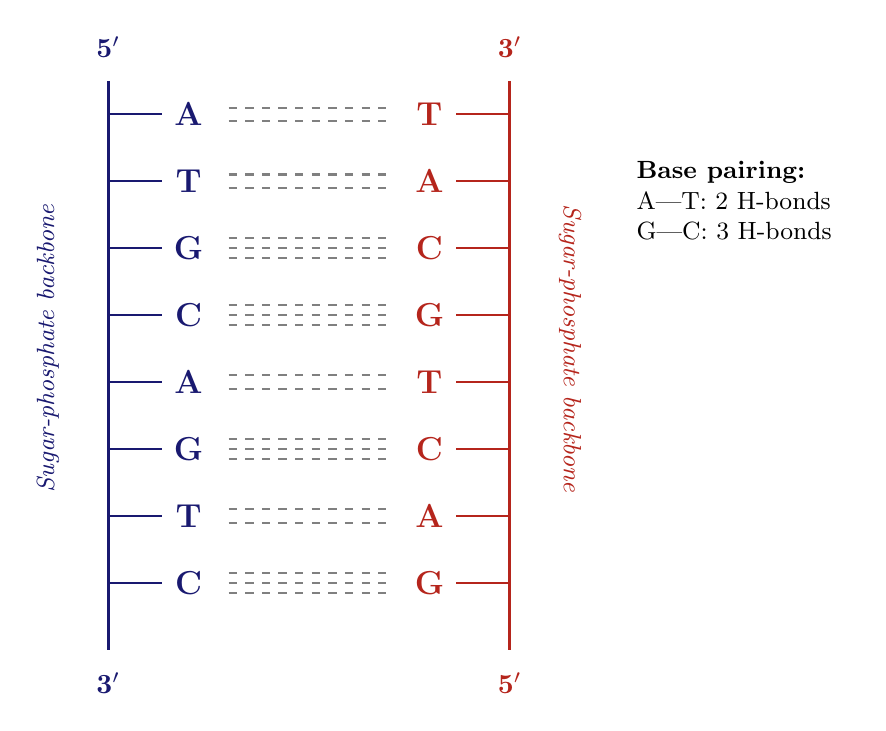
\begin{tikzpicture}[scale=0.85]
  % Draw the two backbone strands
  \draw[very thick, MidnightBlue] (0,0) -- (0,-8.5);
  \draw[very thick, BrickRed] (6,0) -- (6,-8.5);

  % Labels for strands
  \node[above, MidnightBlue, font=\bfseries] at (0,0.2) {5$'$};
  \node[below, MidnightBlue, font=\bfseries] at (0,-8.7) {3$'$};
  \node[above, BrickRed, font=\bfseries] at (6,0.2) {3$'$};
  \node[below, BrickRed, font=\bfseries] at (6,-8.7) {5$'$};

  % Base pairs
  \foreach \y/\leftbase/\rightbase/\bonds in {
    -0.5/A/T/2,
    -1.5/T/A/2,
    -2.5/G/C/3,
    -3.5/C/G/3,
    -4.5/A/T/2,
    -5.5/G/C/3,
    -6.5/T/A/2,
    -7.5/C/G/3
  } {
    % Base labels
    \node[MidnightBlue, font=\bfseries\large] at (1.2,\y) {\leftbase};
    \node[BrickRed, font=\bfseries\large] at (4.8,\y) {\rightbase};

    % Hydrogen bonds (dashed lines)
    \ifnum\bonds=2
      \draw[dashed, thick, gray] (1.8,\y+0.1) -- (4.2,\y+0.1);
      \draw[dashed, thick, gray] (1.8,\y-0.1) -- (4.2,\y-0.1);
    \else
      \draw[dashed, thick, gray] (1.8,\y+0.15) -- (4.2,\y+0.15);
      \draw[dashed, thick, gray] (1.8,\y) -- (4.2,\y);
      \draw[dashed, thick, gray] (1.8,\y-0.15) -- (4.2,\y-0.15);
    \fi

    % Connections from backbone to bases
    \draw[thick, MidnightBlue] (0,\y) -- (0.8,\y);
    \draw[thick, BrickRed] (6,\y) -- (5.2,\y);
  }

  % Sugar-phosphate backbone labels
  \node[rotate=90, MidnightBlue, font=\small\itshape] at (-0.9,-4) {Sugar-phosphate backbone};
  \node[rotate=-90, BrickRed, font=\small\itshape] at (6.9,-4) {Sugar-phosphate backbone};

  % Legend
  \node[anchor=north west, font=\small] at (7.5,-1) {
    \begin{tabular}{l}
    \textbf{Base pairing:} \\
    A---T: 2 H-bonds \\
    G---C: 3 H-bonds \\
    \end{tabular}
  };
\end{tikzpicture}
\caption[Simplified DNA structure.]{Simplified representation of DNA double-stranded structure showing the antiparallel sugar-phosphate backbones (blue and red) connected by complementary base pairs via hydrogen bonds (dashed lines). Note that G-C pairs have three hydrogen bonds, making them stronger than A-T pairs (two hydrogen bonds).}
\label{fig:molbio:dna-structure}
\end{figure}


% ============================================================
\section{DNA Organisation: From Double Helix to Chromosome}
\label{sec:molbio:dna-organisation}

The human genome contains approximately 3.2 billion base pairs of DNA. If stretched out, the DNA from a single human cell would be about 2 metres long. Yet it must fit inside a nucleus roughly 6 micrometres in diameter---a packing ratio of over 300,000 to 1. This remarkable feat of organisation is achieved through a hierarchy of packaging structures.

\subsection{Histones and Nucleosomes}
\label{subsec:molbio:nucleosomes}

The first level of packaging involves proteins called \textbf{histones}. DNA wraps around complexes of eight histone proteins (an \textbf{octamer} composed of two copies each of histones H2A, H2B, H3, and H4) to form structures called \textbf{nucleosomes}. Each nucleosome contains approximately 147 base pairs of DNA wrapped in 1.65 turns around the histone octamer, connected by short stretches of \textbf{linker DNA} (typically 20--60\basepair{}).

A fifth histone, \textbf{H1} (the linker histone), binds to the DNA as it enters and exits the nucleosome, helping to stabilise higher-order structures.

\subsection{Chromatin: Euchromatin and Heterochromatin}
\label{subsec:molbio:chromatin}

The chain of nucleosomes is called \textbf{chromatin}. Chromatin exists in two broad states:

\begin{itemize}[itemsep=2pt]
  \item \textbf{Euchromatin:} Loosely packed, ``open'' chromatin. Genes in euchromatic regions are generally accessible to the transcription machinery and may be actively expressed. Euchromatin appears light in electron microscopy.
  \item \textbf{Heterochromatin:} Tightly packed, ``closed'' chromatin. Genes in heterochromatic regions are generally silenced. Heterochromatin appears dark in electron microscopy. It can be further divided into:
  \begin{itemize}
    \item \textbf{Constitutive heterochromatin:} Permanently condensed regions, often found at centromeres and telomeres, typically containing repetitive sequences.
    \item \textbf{Facultative heterochromatin:} Regions that can switch between open and closed states depending on cell type or developmental stage. The inactive X chromosome in female mammals is a classic example.
  \end{itemize}
\end{itemize}

\subsection{Higher-Order Structures and Chromosomes}
\label{subsec:molbio:chromosomes}

Nucleosomes are further organised into higher-order structures. During cell division (mitosis or meiosis), chromatin condenses maximally into the dense, compact structures visible under a light microscope as \textbf{chromosomes}. Each chromosome consists of a single, continuous DNA molecule complexed with histones and other proteins.

Key chromosome structures include:
\begin{itemize}[itemsep=2pt]
  \item \textbf{Centromere:} The constricted region where the two sister chromatids are joined and where the spindle fibres attach during cell division.
  \item \textbf{Telomeres:} Repetitive DNA sequences (TTAGGG in humans) that cap the ends of chromosomes, protecting them from degradation and preventing them from fusing with neighbouring chromosomes.
\end{itemize}

\subsection{Ploidy}
\label{subsec:molbio:ploidy}

\textbf{Ploidy} refers to the number of complete sets of chromosomes in a cell. Most human somatic (body) cells are \textbf{diploid} (2n)---they contain two copies of each chromosome, one inherited from each parent. Human diploid cells have 46 chromosomes (23 pairs). Gametes (sperm and egg cells) are \textbf{haploid} (n), containing only 23 chromosomes. Some organisms, particularly plants, can be \textbf{polyploid} (e.g., wheat is hexaploid, with six copies of each chromosome), which adds complexity to genome assembly.

% TikZ: Chromatin organisation hierarchy
\begin{figure}[htbp]
\centering
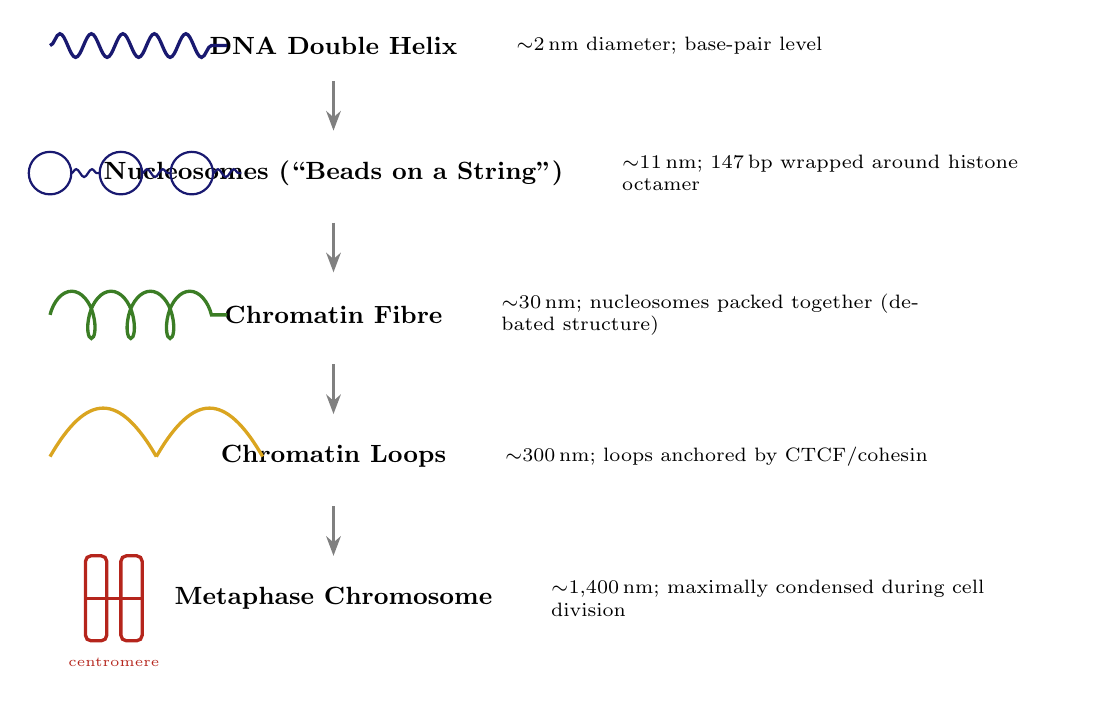
\begin{tikzpicture}[
  level/.style={font=\small\bfseries},
  desc/.style={font=\scriptsize, text width=5.5cm},
  arrow/.style={-{Stealth[length=2.5mm]}, thick, gray},
  scale=0.9
]
  % Level 1: DNA double helix
  \node[level] (dna) at (0,0) {DNA Double Helix};
  \node[desc, right=0.5cm of dna] {$\sim$2\,nm diameter; base-pair level};
  \draw[very thick, MidnightBlue, decorate, decoration={snake, amplitude=1.5mm, segment length=4mm}]
    (-4,0) -- (-1.5,0);

  % Arrow down
  \draw[arrow] (0,-0.5) -- (0,-1.2);

  % Level 2: Nucleosome (beads on a string)
  \node[level] (nuc) at (0,-1.8) {Nucleosomes (``Beads on a String'')};
  \node[desc, right=0.5cm of nuc] {$\sim$11\,nm; 147\,bp wrapped around histone octamer};
  \foreach \x in {-4, -3, -2} {
    \draw[thick, MidnightBlue] (\x,-1.8) circle (0.3);
    \draw[thick, MidnightBlue, decorate, decoration={snake, amplitude=0.5mm, segment length=2mm}]
      (\x+0.3,-1.8) -- (\x+0.7,-1.8);
  }

  % Arrow down
  \draw[arrow] (0,-2.5) -- (0,-3.2);

  % Level 3: 30nm fibre
  \node[level] (fibre) at (0,-3.8) {Chromatin Fibre};
  \node[desc, right=0.5cm of fibre] {$\sim$30\,nm; nucleosomes packed together (debated structure)};
  \draw[very thick, OliveGreen, decorate, decoration={coil, amplitude=3mm, segment length=5mm}]
    (-4,-3.8) -- (-1.5,-3.8);

  % Arrow down
  \draw[arrow] (0,-4.5) -- (0,-5.2);

  % Level 4: Loops
  \node[level] (loop) at (0,-5.8) {Chromatin Loops};
  \node[desc, right=0.5cm of loop] {$\sim$300\,nm; loops anchored by CTCF/cohesin};
  \draw[very thick, Goldenrod] (-4,-5.8) to[out=60,in=120, looseness=1.8] (-2.5,-5.8);
  \draw[very thick, Goldenrod] (-2.5,-5.8) to[out=60,in=120, looseness=1.8] (-1,-5.8);

  % Arrow down
  \draw[arrow] (0,-6.5) -- (0,-7.2);

  % Level 5: Chromosome
  \node[level] (chr) at (0,-7.8) {Metaphase Chromosome};
  \node[desc, right=0.5cm of chr] {$\sim$1,400\,nm; maximally condensed during cell division};
  % Simple chromosome shape
  \draw[very thick, BrickRed, rounded corners=2pt]
    (-3.5,-7.2) -- (-3.5,-8.4) -- (-3.2,-8.4) -- (-3.2,-7.2) -- cycle;
  \draw[very thick, BrickRed, rounded corners=2pt]
    (-3.0,-7.2) -- (-3.0,-8.4) -- (-2.7,-8.4) -- (-2.7,-7.2) -- cycle;
  % Centromere
  \draw[very thick, BrickRed] (-3.5,-7.8) -- (-2.7,-7.8);
  \node[font=\tiny, BrickRed] at (-3.1,-8.7) {centromere};

\end{tikzpicture}
\caption[Chromatin organisation hierarchy.]{The hierarchy of DNA packaging from the naked double helix ($\sim$2\,nm) through nucleosomes ($\sim$11\,nm), chromatin fibres ($\sim$30\,nm), looped domains ($\sim$300\,nm), to the maximally condensed metaphase chromosome ($\sim$1,400\,nm). Each level of organisation has implications for gene regulation and is measurable by specific sequencing assays (e.g., \acrshort{ATAC-seq} for nucleosome positioning, \acrshort{Hi-C} for looping interactions).}
\label{fig:molbio:chromatin-hierarchy}
\end{figure}


% ============================================================
\section{Genes and the Genome}
\label{sec:molbio:genes-genome}

\subsection{What Is a Gene?}
\label{subsec:molbio:gene-definition}

A \textbf{gene} is a segment of DNA that contains the instructions for producing a functional product---usually a protein, but in some cases a functional RNA molecule. The human genome contains approximately 20,000--25,000 protein-coding genes, but these account for only about 1.5\% of the total genome. The rest---once dismissively called ``junk DNA''---includes regulatory sequences, non-coding RNAs, repetitive elements, and regions of unknown function.

\subsection{Gene Structure: Exons and Introns}
\label{subsec:molbio:exons-introns}

In eukaryotes, most protein-coding genes have a \textbf{split structure}: the coding sequence is divided into segments called \textbf{exons}, separated by non-coding sequences called \textbf{introns}. When the gene is transcribed, the entire region (exons + introns) is copied into a precursor RNA molecule (pre-mRNA). The introns are then removed through a process called \textbf{splicing}, and the exons are joined together to form the mature mRNA (see \cref{subsec:molbio:transcription}).

This arrangement allows for \textbf{alternative splicing}: different combinations of exons can be included in the final mRNA, producing different protein variants (called \textbf{isoforms}) from a single gene. Alternative splicing dramatically increases the diversity of proteins that can be produced from a finite number of genes. It is estimated that over 95\% of human multi-exon genes undergo alternative splicing.

\subsection{Regulatory Regions}
\label{subsec:molbio:regulatory-regions}

Genes do not exist in isolation---their expression is controlled by \textbf{regulatory DNA elements}:

\begin{description}[style=nextline, itemsep=3pt]
  \item[Promoter] A DNA sequence located immediately upstream (5$'${}) of the gene's transcription start site (TSS). The promoter is where \textbf{RNA polymerase} and general \textbf{transcription factors} bind to initiate transcription. Many promoters contain a TATA box (consensus sequence TATAAA) approximately 25--30\basepair{} upstream of the TSS, though many genes---particularly housekeeping genes---lack a TATA box and instead have CpG-island-associated promoters.

  \item[Enhancer] A regulatory DNA element that can increase transcription of a gene, often located thousands or even millions of base pairs away from the gene it regulates. Enhancers work by binding transcription factors and physically looping to contact the gene's promoter through three-dimensional chromatin folding. Enhancers can function regardless of their orientation or position relative to the gene.

  \item[Silencer] A regulatory element that represses transcription, functioning conceptually as the opposite of an enhancer.

  \item[Insulator] A boundary element that prevents regulatory signals (enhancers, silencers) from affecting genes on the other side of the insulator. The protein CTCF is a key component of many insulator elements.
\end{description}

\subsection{Repetitive Elements}
\label{subsec:molbio:repetitive-elements}

Approximately 45--50\% of the human genome consists of \textbf{repetitive elements}---DNA sequences present in many copies. Major categories include:

\begin{itemize}[itemsep=2pt]
  \item \textbf{SINEs (Short Interspersed Nuclear Elements):} The most common are Alu elements ($\sim$300\basepair{}), with over one million copies in the human genome.
  \item \textbf{LINEs (Long Interspersed Nuclear Elements):} The most common are LINE-1 (L1) elements ($\sim$6\kilobase{}), with about 500,000 copies.
  \item \textbf{DNA transposons:} ``Cut-and-paste'' mobile elements that are mostly inactive in the human genome.
  \item \textbf{Tandem repeats:} Including microsatellites (1--6\basepair{} repeat units, e.g., CACACA\ldots) and minisatellites (longer repeat units).
  \item \textbf{Segmental duplications:} Large blocks (>1\kilobase{}) of DNA that are duplicated, often in different locations in the genome.
\end{itemize}

\begin{warningbox}
Repetitive regions pose a major challenge for sequencing and genome assembly. Short sequencing reads originating from repetitive elements cannot be unambiguously placed in the genome, leading to ``multi-mapping'' reads and assembly gaps. Long-read sequencing technologies (\cref{ch:seqprinciples}) have significantly improved our ability to resolve repetitive regions.
\end{warningbox}

\subsection{Coding vs.\ Non-Coding DNA}
\label{subsec:molbio:coding-noncoding}

A common misconception is that most DNA ``does something'' by encoding proteins. In fact, the situation is far more nuanced:

\begin{itemize}[itemsep=2pt]
  \item $\sim$1.5\% of the human genome encodes protein sequences (exons of protein-coding genes).
  \item $\sim$5--10\% is estimated to be under evolutionary constraint (functional, including regulatory elements and non-coding RNAs), based on comparative genomics.
  \item $\sim$45--50\% consists of repetitive and transposable elements.
  \item The function (or lack thereof) of the remaining DNA is an active area of research.
\end{itemize}


% ============================================================
\section{The Central Dogma of Molecular Biology}
\label{sec:molbio:central-dogma}

In 1958, Francis Crick articulated what he called the \textbf{Central Dogma of molecular biology}: the principle that genetic information flows from DNA to RNA to protein. While we now know of exceptions and nuances (reverse transcription, RNA editing, prions), this framework remains the core organising principle of molecular biology.

% TikZ: Central Dogma diagram
\begin{figure}[htbp]
\centering
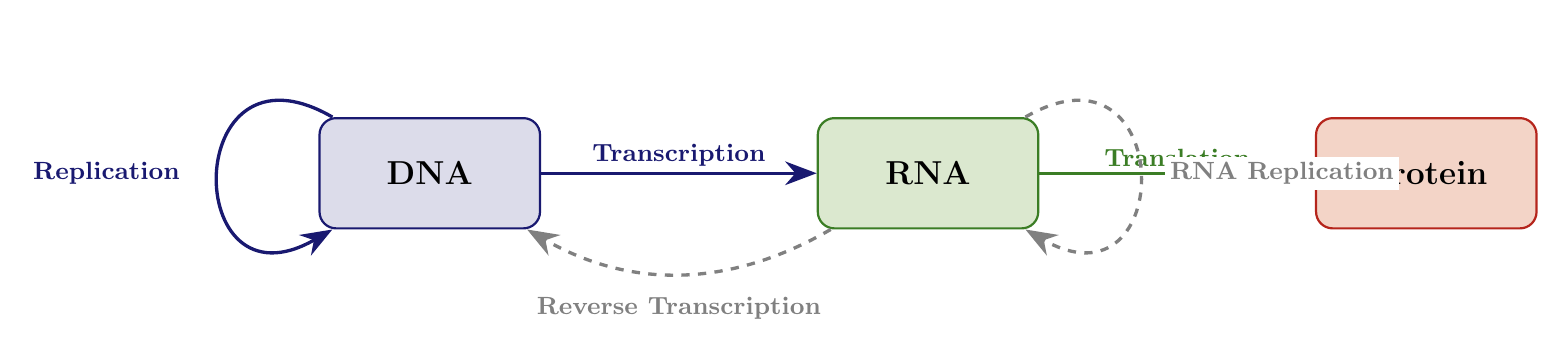
\begin{tikzpicture}[
  node distance=3.5cm,
  mol/.style={
    draw, rounded corners=6pt, thick,
    minimum width=2.8cm, minimum height=1.4cm,
    align=center, font=\large\bfseries
  },
  process/.style={font=\small\bfseries, fill=white, inner sep=2pt},
  arrow/.style={-{Stealth[length=4mm]}, very thick},
]
  % Molecules
  \node[mol, fill=MidnightBlue!15, draw=MidnightBlue] (dna) {DNA};
  \node[mol, fill=OliveGreen!15, draw=OliveGreen, right=of dna] (rna) {RNA};
  \node[mol, fill=BrickRed!15, draw=BrickRed, right=of rna] (protein) {Protein};

  % Main arrows
  \draw[arrow, MidnightBlue] (dna) -- node[process, above] {Transcription} (rna);
  \draw[arrow, OliveGreen] (rna) -- node[process, above] {Translation} (protein);

  % DNA replication (self-loop)
  \draw[arrow, MidnightBlue] (dna) to[out=150, in=210, looseness=4]
    node[process, left, xshift=-4mm] {Replication} (dna);

  % Reverse transcription (dashed)
  \draw[arrow, dashed, gray] (rna) to[out=210, in=-30]
    node[process, below, yshift=-2mm] {\color{gray}Reverse Transcription} (dna);

  % RNA replication (for RNA viruses)
  \draw[arrow, dashed, gray] (rna) to[out=30, in=-30, looseness=4]
    node[process, right, xshift=3mm] {\color{gray}RNA Replication} (rna);

\end{tikzpicture}
\caption[The Central Dogma of molecular biology.]{The Central Dogma: genetic information flows from DNA to RNA (transcription) to protein (translation). DNA can also be replicated. Dashed arrows indicate processes that occur in special contexts: reverse transcription (used by retroviruses and retrotransposons) and RNA-dependent RNA replication (used by some RNA viruses).}
\label{fig:molbio:central-dogma}
\end{figure}

The Central Dogma (\cref{fig:molbio:central-dogma}) describes three main processes:

\begin{enumerate}[itemsep=3pt]
  \item \textbf{Replication:} DNA $\rightarrow$ DNA. The faithful copying of the genome before cell division.
  \item \textbf{Transcription:} DNA $\rightarrow$ RNA. A gene's DNA sequence is copied into a messenger RNA (mRNA) molecule.
  \item \textbf{Translation:} RNA $\rightarrow$ Protein. The mRNA sequence is decoded by ribosomes to produce a chain of amino acids (a polypeptide) that folds into a functional protein.
\end{enumerate}


\subsection{Kinetics of Information Flow}
\label{subsec:molbio:kinetics}

The speed and fidelity of the enzymes that execute the Central Dogma are directly relevant to sequencing, because many sequencing chemistries harness these same enzymes (or engineered variants of them). \Cref{tab:molbio:polymerase-kinetics} summarises the key kinetic parameters.

\begin{table}[htbp]
\centering
\caption[Polymerase kinetics comparison.]{Kinetic parameters of the major polymerases involved in information flow. Processivity is the average number of nucleotides incorporated before the enzyme dissociates.}
\label{tab:molbio:polymerase-kinetics}
\small
\begin{tabularx}{\textwidth}{>{\bfseries}l X r r r}
\toprule
\textbf{Enzyme} & \textbf{Function} & \textbf{Speed (nt/s)} & \textbf{Error rate} & \textbf{Processivity} \\
\midrule
\species{E.~coli} DNA Pol III & Replication & 1,000 & $10^{-7}$ & $>$500,000 \\
\addlinespace
Human DNA Pol $\delta$ & Replication (lagging) & 30--50 & $10^{-7}$ & $\sim$500 \\
\addlinespace
Human DNA Pol $\varepsilon$ & Replication (leading) & 50--100 & $10^{-6}$--$10^{-7}$ & $>$10,000 \\
\addlinespace
Phi29 DNA Pol & Isothermal amplification & 25--50 & $10^{-6}$ & $>$70,000 \\
\addlinespace
\species{E.~coli} RNA Pol & Transcription & 40--80 & $10^{-4}$--$10^{-5}$ & $\sim$10,000 \\
\addlinespace
Human RNA Pol II & Transcription & 20--50 & $10^{-4}$--$10^{-5}$ & Variable \\
\addlinespace
Ribosome & Translation (aa/s) & 5--20 & $10^{-3}$--$10^{-4}$ & Complete mRNA \\
\bottomrule
\end{tabularx}
\end{table}

Several insights emerge from these kinetics:

\begin{itemize}[itemsep=2pt]
  \item \textbf{Replication is extraordinarily accurate.} After proofreading ($3' \rightarrow 5'$ exonuclease activity), replicative DNA polymerases achieve error rates of $\sim$$10^{-7}$ per base pair. With post-replication mismatch repair, the overall error rate drops to $\sim$$10^{-9}$--$10^{-10}$ per base pair per cell division.
  \item \textbf{Transcription is 100--1,000$\times$ less accurate} than replication. This is tolerable because (1) each transcript is temporary, (2) many copies of each mRNA are made, and (3) errors in any single transcript are diluted by the population.
  \item \textbf{Sequencing-by-synthesis co-opts polymerase chemistry.} The Phi29 polymerase (used in PacBio SMRT sequencing) combines high processivity ($>$70,000 nt) with moderate speed and good accuracy---ideal for long, continuous reads. Understanding these enzymatic parameters explains why different platforms achieve different read lengths and error rates.
\end{itemize}

\begin{keyconcept}[title={Fidelity Hierarchy}]
Information fidelity decreases at each step of the Central Dogma: DNA replication ($\sim$$10^{-10}$ errors/bp after repair) $>$ transcription ($\sim$$10^{-5}$ errors/nt) $>$ translation ($\sim$$10^{-4}$ errors/aa). This hierarchy reflects biological priorities: the genome must be copied with near-perfect fidelity across generations, while temporary RNA and protein errors are tolerable.
\end{keyconcept}


% ============================================================
\section{Transcription: From DNA to RNA}
\label{sec:molbio:transcription}

\textbf{Transcription} is the process of synthesising an RNA copy of a gene's DNA sequence. It is carried out by the enzyme \textbf{RNA polymerase}, which reads the template strand of DNA (3$'${} $\rightarrow$ 5$'${}) and synthesises a complementary RNA strand in the 5$'${} $\rightarrow$ 3$'${} direction.

\subsection{Transcription in Eukaryotes}
\label{subsec:molbio:euk-transcription}

Eukaryotic transcription is more complex than prokaryotic transcription and involves three main RNA polymerases:

\begin{itemize}[itemsep=2pt]
  \item \textbf{RNA Polymerase I:} Transcribes ribosomal RNA (rRNA) genes (except 5S rRNA).
  \item \textbf{RNA Polymerase II:} Transcribes messenger RNA (mRNA) and most non-coding RNAs, including miRNAs and lncRNAs. This is the polymerase most relevant to gene expression studies.
  \item \textbf{RNA Polymerase III:} Transcribes transfer RNAs (tRNAs), 5S rRNA, and other small RNAs.
\end{itemize}

The process of mRNA transcription by RNA Polymerase II occurs in three stages:

\begin{description}[style=nextline, itemsep=3pt]
  \item[Initiation] General transcription factors (TFIIA, TFIIB, TFIID, TFIIE, TFIIF, TFIIH) assemble at the promoter, forming the \textbf{preinitiation complex}. TFIID recognises and binds the TATA box (via its TBP subunit). RNA Polymerase II is recruited, and the DNA double helix is unwound (``melted'') at the transcription start site.

  \item[Elongation] RNA Polymerase II moves along the template strand, synthesising mRNA in the 5$'${} $\rightarrow$ 3$'${} direction. The RNA transcript is complementary to the template strand and identical in sequence to the coding (sense) strand, except that uracil (U) replaces thymine (T).

  \item[Termination] Transcription continues past the end of the coding sequence until specific termination signals are reached. In eukaryotes, the pre-mRNA is cleaved and polyadenylated (see below), and the polymerase dissociates from the DNA.
\end{description}

\subsection{mRNA Processing}
\label{subsec:molbio:mrna-processing}

In eukaryotes, the initial transcript (pre-mRNA) undergoes three critical processing steps before it can serve as a template for protein synthesis:

\begin{enumerate}[itemsep=3pt]
  \item \textbf{5$'${} Capping:} A modified guanine nucleotide (7-methylguanosine, m$^7$G) is added to the 5$'${} end of the pre-mRNA. The 5$'${} cap protects the mRNA from degradation, facilitates ribosome binding during translation, and aids in nuclear export.

  \item \textbf{Splicing:} Introns are removed and exons are joined together by a large ribonucleoprotein complex called the \textbf{spliceosome}. The spliceosome recognises specific sequences at intron--exon boundaries: the \textbf{5$'${} splice site} (donor site, typically GU), the \textbf{3$'${} splice site} (acceptor site, typically AG), and the \textbf{branch point} (an adenosine within the intron). As mentioned earlier, alternative splicing can produce different mRNA isoforms from the same gene.

  \item \textbf{3$'${} Polyadenylation:} A tail of 100--250 adenine nucleotides (the \textbf{poly-A tail}) is added to the 3$'${} end of the mRNA. The poly-A tail protects the mRNA from degradation, facilitates nuclear export, and aids in translation. In many \acrshort{RNA-seq} protocols, the poly-A tail is used to selectively capture mRNA from the total RNA pool (poly-A selection).
\end{enumerate}

\begin{tipbox}
The poly-A tail is exploited in many RNA sequencing library preparation protocols. Oligo-dT beads (short chains of thymine nucleotides) are used to capture mRNAs via their poly-A tails, enriching for mRNA and depleting abundant ribosomal RNA. However, this approach misses non-polyadenylated RNAs (such as many histone mRNAs and most non-coding RNAs). If your experiment aims to study non-coding RNAs, consider rRNA depletion instead of poly-A selection.
\end{tipbox}


% ============================================================
\section{Translation: From RNA to Protein}
\label{sec:molbio:translation}

\textbf{Translation} is the process by which the nucleotide sequence of an mRNA is decoded to produce a polypeptide (protein). This process takes place on \textbf{ribosomes}---complex molecular machines composed of ribosomal RNA (rRNA) and proteins.

\subsection{The Genetic Code}
\label{subsec:molbio:genetic-code}

The genetic code is the set of rules by which the nucleotide sequence of mRNA is translated into the amino acid sequence of a protein. The code is read in \textbf{triplets} called \textbf{codons}: each codon (a sequence of three nucleotides) specifies one amino acid or a stop signal.

Key properties of the genetic code:
\begin{itemize}[itemsep=2pt]
  \item \textbf{64 codons} encode 20 standard amino acids plus 3 stop signals. Because there are more codons than amino acids, the code is \textbf{degenerate} (redundant): most amino acids are specified by more than one codon.
  \item \textbf{AUG} (encoding methionine) serves as the \textbf{start codon}, signalling the beginning of translation.
  \item \textbf{UAA, UAG, UGA} are \textbf{stop codons}, signalling the end of translation.
  \item The code is nearly \textbf{universal}: the same codons specify the same amino acids in virtually all organisms, from bacteria to humans (with minor exceptions in mitochondria and a few organisms).
\end{itemize}

\subsection{The Process of Translation}
\label{subsec:molbio:translation-process}

Translation occurs in three phases:

\begin{description}[style=nextline, itemsep=3pt]
  \item[Initiation] The small ribosomal subunit binds to the mRNA and scans for the start codon (AUG). A special initiator tRNA carrying methionine base-pairs with the start codon. The large ribosomal subunit then joins to form the complete ribosome.

  \item[Elongation] The ribosome moves along the mRNA in the 5$'${} $\rightarrow$ 3$'${} direction, reading one codon at a time. For each codon, a \textbf{transfer RNA (tRNA)} molecule carrying the corresponding amino acid binds to the ribosome via complementary base pairing between the codon and the tRNA's \textbf{anticodon}. The amino acid is added to the growing polypeptide chain via a \textbf{peptide bond}.

  \item[Termination] When the ribosome reaches a stop codon, \textbf{release factors} bind and trigger the release of the completed polypeptide. The ribosome dissociates from the mRNA.
\end{description}

\subsection{Protein Folding and Function}
\label{subsec:molbio:protein-folding}

The newly synthesised polypeptide chain folds into a specific three-dimensional structure determined by its amino acid sequence. This folding occurs at multiple levels:

\begin{itemize}[itemsep=2pt]
  \item \textbf{Primary structure:} The linear sequence of amino acids.
  \item \textbf{Secondary structure:} Local folding patterns, mainly \textbf{alpha helices} and \textbf{beta sheets}, stabilised by hydrogen bonds.
  \item \textbf{Tertiary structure:} The overall three-dimensional shape of a single polypeptide, stabilised by hydrophobic interactions, hydrogen bonds, ionic bonds, and disulfide bridges.
  \item \textbf{Quaternary structure:} The arrangement of multiple polypeptide subunits into a multi-subunit complex (e.g., haemoglobin is a tetramer of four polypeptide chains).
\end{itemize}

A protein's function depends critically on its three-dimensional structure. Mutations that alter the amino acid sequence can disrupt folding and cause disease.


% ============================================================
\section{Types of RNA}
\label{sec:molbio:rna-types}

While mRNA is the most commonly studied RNA in sequencing experiments, cells produce a diverse array of RNA molecules with different functions:

\begin{description}[style=nextline, itemsep=3pt]
  \item[Messenger RNA (mRNA)] Encodes the amino acid sequence of proteins. Represents approximately 3--5\% of total cellular RNA by mass but is the most informationally diverse RNA class. This is the primary target of \acrshort{RNA-seq} experiments.

  \item[Ribosomal RNA (rRNA)] The catalytic and structural RNA component of ribosomes. Comprises approximately 80--85\% of total cellular RNA. In \acrshort{RNA-seq} experiments, rRNA is either depleted or excluded via poly-A selection; otherwise, the vast majority of reads would come from rRNA.

  \item[Transfer RNA (tRNA)] Small adapter molecules ($\sim$75--90 nucleotides) that carry amino acids to the ribosome during translation. Each tRNA has an anticodon that pairs with the corresponding mRNA codon.

  \item[MicroRNA (miRNA)] Small non-coding RNAs ($\sim$22 nucleotides) that regulate gene expression post-transcriptionally by binding to complementary sequences in the 3$'${} untranslated regions (3$'${} UTR) of target mRNAs, leading to mRNA degradation or translational repression. A single miRNA can regulate hundreds of target genes.

  \item[Long non-coding RNA (lncRNA)] Non-coding RNAs longer than 200 nucleotides with diverse roles in gene regulation, chromatin remodelling, and nuclear organisation. Examples include XIST (involved in X-chromosome inactivation) and HOTAIR (involved in chromatin remodelling). Thousands of lncRNAs have been identified, but the functions of most remain unknown.

  \item[Circular RNA (circRNA)] Covalently closed circular RNA molecules formed by back-splicing, in which a downstream splice donor joins to an upstream splice acceptor. circRNAs are resistant to exonucleolytic degradation and have been implicated as miRNA sponges, protein scaffolds, and regulators of transcription.

  \item[Piwi-interacting RNA (piRNA)] Small RNAs ($\sim$24--32 nucleotides) that interact with Piwi proteins and function primarily in transposon silencing in the germline.

  \item[Small nuclear RNA (snRNA)] Components of the spliceosome; essential for pre-mRNA splicing (e.g., U1, U2, U4, U5, U6 snRNAs).

  \item[Small nucleolar RNA (snoRNA)] Guide chemical modifications (methylation and pseudouridylation) of rRNA and other RNAs.
\end{description}

\begin{keyconcept}[title={RNA Diversity}]
The transcriptome is far more complex than just mRNA. Non-coding RNAs constitute the vast majority of cellular RNA and play critical roles in gene regulation, splicing, translation, and genome defence. Modern sequencing technologies can profile all of these RNA classes, but different library preparation methods are needed for different RNA types.
\end{keyconcept}


% ============================================================
\section{Epigenetics: Modifications Beyond the Sequence}
\label{sec:molbio:epigenetics}

\textbf{Epigenetics} refers to heritable changes in gene expression that occur without changes to the underlying DNA sequence. Epigenetic mechanisms control which genes are active in which cell types, and their dysregulation is implicated in cancer, developmental disorders, and ageing.

\subsection{DNA Methylation}
\label{subsec:molbio:dna-methylation}

\textbf{DNA methylation} is the addition of a methyl group ($-$CH$_3$) to the carbon-5 position of cytosine, producing \textbf{5-methylcytosine (5mC)}. In mammals, this modification occurs predominantly at \textbf{CpG dinucleotides}---positions where a cytosine is immediately followed by a guanine on the same strand.

Key points about DNA methylation:
\begin{itemize}[itemsep=2pt]
  \item \textbf{CpG islands:} Regions of the genome with a high density of CpG dinucleotides (typically >200\basepair{}, with observed/expected CpG ratio >0.6 and GC content >50\%). CpG islands are found at approximately 70\% of human gene promoters.
  \item \textbf{Gene silencing:} Methylation of CpG islands in promoter regions is generally associated with \textbf{transcriptional silencing}. Methylated promoters recruit proteins that compact chromatin, making genes inaccessible to the transcription machinery.
  \item \textbf{Maintenance and \textit{de novo} methylation:} DNA methyltransferase 1 (DNMT1) maintains methylation patterns during DNA replication by copying methyl marks from the parent strand to the newly synthesised strand. DNMT3A and DNMT3B establish new (``\textit{de novo}'') methylation patterns.
  \item \textbf{Demethylation:} Active demethylation involves oxidation of 5mC to 5-hydroxymethylcytosine (5hmC), 5-formylcytosine (5fC), and 5-carboxylcytosine (5caC) by TET (Ten-eleven translocation) enzymes, followed by base excision repair.
\end{itemize}

DNA methylation can be measured genome-wide using \acrshort{WGBS}, which treats DNA with sodium bisulfite to convert unmethylated cytosines to uracil (read as thymine after \acrshort{PCR}) while leaving methylated cytosines unchanged. This is discussed in detail in later chapters.

\subsection{Histone Modifications}
\label{subsec:molbio:histone-mods}

Histones are not merely passive spools for DNA packaging. The N-terminal ``tails'' of histone proteins protrude from the nucleosome and can be chemically modified at specific amino acid residues. These modifications---collectively called \textbf{histone marks}---influence chromatin structure and gene expression.

Major types of histone modifications include:

\begin{itemize}[itemsep=2pt]
  \item \textbf{Acetylation} (e.g., H3K27ac, H3K9ac): Addition of an acetyl group, generally associated with active gene expression. Acetylation neutralises the positive charge of lysine residues, loosening the interaction between histones and negatively charged DNA.
  \item \textbf{Methylation} (e.g., H3K4me3, H3K36me3, H3K27me3, H3K9me3): Addition of one, two, or three methyl groups to lysine or arginine residues. Unlike acetylation, methylation can be associated with either activation or repression, depending on the specific residue and the degree of methylation:
  \begin{itemize}
    \item H3K4me3 (trimethylation of lysine 4 on histone H3): marks \textit{active} promoters.
    \item H3K27me3: marks \textit{repressed} genes (Polycomb repression).
    \item H3K9me3: marks \textit{constitutive heterochromatin}.
    \item H3K36me3: marks \textit{actively transcribed} gene bodies.
  \end{itemize}
  \item \textbf{Phosphorylation} (e.g., H3S10ph): Addition of a phosphate group. Associated with chromosome condensation during mitosis and with transcriptional activation.
  \item \textbf{Ubiquitylation} (e.g., H2AK119ub, H2BK120ub): Addition of the small protein ubiquitin. Involved in both activation and repression.
\end{itemize}

The combination of histone modifications at a given genomic locus constitutes what is sometimes called the \textbf{histone code}---a complex regulatory layer that is read by effector proteins to control gene expression. These modifications can be mapped genome-wide using \acrshort{ChIP-seq} and related techniques (see later chapters).

\subsection{Chromatin Remodelling}
\label{subsec:molbio:chromatin-remodelling}

In addition to covalent modifications, chromatin structure is actively remodelled by \textbf{ATP-dependent chromatin remodelling complexes} (such as SWI/SNF, ISWI, CHD, and INO80 families). These enzymes use the energy of ATP hydrolysis to slide, eject, or restructure nucleosomes, thereby altering the accessibility of DNA to transcription factors and other regulatory proteins. Chromatin accessibility can be measured genome-wide using \acrshort{ATAC-seq} (see later chapters).

\begin{keyconcept}[title={The Epigenome as a Regulatory Layer}]
The epigenome---comprising DNA methylation, histone modifications, and chromatin accessibility---acts as a regulatory layer on top of the DNA sequence. It determines which genes are active in which cell types, without changing the genetic code itself. Every cell in your body (with rare exceptions) has the same genome, but different epigenomes are what make a neuron different from a liver cell. Modern sequencing technologies can map each of these epigenetic marks at single-nucleotide or single-cell resolution.
\end{keyconcept}


% ============================================================
\section{DNA Replication and Repair}
\label{sec:molbio:replication-repair}

\subsection{DNA Replication}
\label{subsec:molbio:replication}

Before a cell divides, it must duplicate its entire genome so that each daughter cell receives a complete copy. \textbf{DNA replication} is the process by which the double-stranded DNA molecule is copied. Key features include:

\begin{itemize}[itemsep=2pt]
  \item \textbf{Semi-conservative:} Each daughter DNA molecule contains one original (parental) strand and one newly synthesised strand. This was demonstrated by the famous Meselson--Stahl experiment in 1958.
  \item \textbf{Bidirectional:} Replication proceeds in both directions from each \textbf{origin of replication}. Eukaryotic genomes have thousands of origins to ensure the entire genome is replicated within the S phase of the cell cycle.
  \item \textbf{Key enzymes:}
  \begin{itemize}
    \item \textbf{Helicase:} Unwinds the double helix at the replication fork.
    \item \textbf{Primase:} Synthesises short RNA primers to provide a 3$'${}-OH group for DNA polymerase.
    \item \textbf{DNA polymerase:} Synthesises new DNA in the 5$'${} $\rightarrow$ 3$'${} direction, adding nucleotides complementary to the template strand. DNA polymerase cannot start synthesis \textit{de novo}---it can only extend an existing primer.
    \item \textbf{Ligase:} Joins Okazaki fragments on the lagging strand.
  \end{itemize}
  \item \textbf{Leading and lagging strands:} Because DNA polymerase can only synthesise in the 5$'${} $\rightarrow$ 3$'${} direction but the two template strands run antiparallel, replication is continuous on the \textbf{leading strand} (synthesised in the direction of fork movement) and discontinuous on the \textbf{lagging strand} (synthesised in short fragments called \textbf{Okazaki fragments} that are later joined).
  \item \textbf{Proofreading:} DNA polymerases have a 3$'${} $\rightarrow$ 5$'${} exonuclease activity that allows them to correct errors immediately, achieving an error rate of approximately one mistake per $10^{9}$--$10^{10}$ base pairs replicated.
\end{itemize}

\subsection{DNA Repair}
\label{subsec:molbio:repair}

DNA is constantly damaged by environmental factors (UV radiation, chemical mutagens) and by-products of normal metabolism (reactive oxygen species). Cells have evolved multiple DNA repair pathways:

\begin{itemize}[itemsep=2pt]
  \item \textbf{Mismatch repair (MMR):} Corrects base-pairing errors that escape proofreading during replication.
  \item \textbf{Base excision repair (BER):} Repairs small, non-helix-distorting lesions (e.g., oxidised or deaminated bases).
  \item \textbf{Nucleotide excision repair (NER):} Repairs bulky, helix-distorting lesions (e.g., thymine dimers caused by UV light).
  \item \textbf{Homologous recombination (HR):} Repairs double-strand breaks using the homologous chromosome or sister chromatid as a template. This is a high-fidelity repair mechanism.
  \item \textbf{Non-homologous end joining (NHEJ):} Repairs double-strand breaks by directly ligating the broken ends together. This is faster but more error-prone than HR, as it can introduce small insertions or deletions.
\end{itemize}

Defects in DNA repair pathways are associated with increased mutation rates and cancer predisposition. For example, mutations in BRCA1 and BRCA2 (which function in homologous recombination) dramatically increase the risk of breast and ovarian cancer.


% ============================================================
\section{Genetic Variation}
\label{sec:molbio:genetic-variation}

No two individuals (except identical twins) have exactly the same genome. The differences between individual genomes---collectively called \textbf{genetic variation}---are the raw material for evolution and the basis for individual traits, disease susceptibility, and pharmacological response. Understanding the types of genetic variation is essential for interpreting sequencing data.

\subsection{Single Nucleotide Polymorphisms (SNPs)}
\label{subsec:molbio:snps}

A \textbf{\acrfull{SNP}} is a position in the genome where a single nucleotide differs between individuals (or between the two copies of a chromosome within an individual). SNPs are the most common type of genetic variation. The human genome contains approximately 4--5 million SNPs per individual (compared to the reference genome), occurring roughly once every 600--1,000 base pairs.

Most SNPs have no functional consequence (they occur in non-coding, non-regulatory regions). However, some SNPs can:
\begin{itemize}[itemsep=2pt]
  \item Alter the amino acid sequence of a protein (missense variants).
  \item Create a premature stop codon (nonsense variants).
  \item Affect gene regulatory elements (eQTLs---expression quantitative trait loci).
  \item Influence splicing (splice site variants).
\end{itemize}

\subsection{Insertions and Deletions (Indels)}
\label{subsec:molbio:indels}

\textbf{\Acrfullpl{indel}} are genetic variants in which one or more nucleotides are inserted into or deleted from the genome. Short indels (1--50\basepair{}) are the second most common type of variation. Indels in protein-coding regions can cause \textbf{frameshift mutations} if their length is not a multiple of three, disrupting the reading frame of the gene and typically rendering the protein non-functional.

\subsection{Structural Variants (SVs)}
\label{subsec:molbio:svs}

\textbf{\Acrfullpl{SV}} are large-scale genomic alterations (typically defined as variants $>$50\basepair{}) that include:

\begin{itemize}[itemsep=2pt]
  \item \textbf{Deletions:} Loss of a segment of DNA.
  \item \textbf{Duplications:} Copying of a segment, resulting in extra copies.
  \item \textbf{Inversions:} Reversal of the orientation of a segment.
  \item \textbf{Translocations:} Transfer of a segment from one chromosome to another.
  \item \textbf{Complex rearrangements:} Combinations of the above.
\end{itemize}

Structural variants affect more total base pairs of the genome than SNPs and indels combined, yet they have historically been harder to detect because short sequencing reads often cannot span them. Long-read sequencing technologies have greatly improved SV detection.

\subsection{Copy Number Variants (CNVs)}
\label{subsec:molbio:cnvs}

\textbf{\Acrfullpl{CNV}} are a subtype of structural variant in which segments of the genome (typically >1\kilobase{}) are present in a variable number of copies. CNVs can encompass entire genes, leading to differences in gene dosage between individuals. Some CNVs are common and benign; others are associated with disease (e.g., the association between CNVs in the \gene{SMN1} gene and spinal muscular atrophy).

\begin{warningbox}
Different types of genetic variation require different sequencing strategies for reliable detection. \acrshort{SNP}s and short indels are well-detected by short-read \acrshort{WGS} at $\geq$30$\times$ coverage. Structural variants and CNVs often require long-read sequencing, linked-read sequencing, or specialised algorithms. No single method detects all variant types with equal sensitivity.
\end{warningbox}


% ============================================================
\section{Gene Regulation: Controlling When and Where Genes Are Expressed}
\label{sec:molbio:gene-regulation}

Not all genes are active in every cell. Gene expression is tightly regulated at multiple levels, from the accessibility of DNA to the stability of mRNA and protein. Understanding gene regulation is essential because many sequencing assays are specifically designed to measure different aspects of this regulation.

\subsection{Transcription Factors}
\label{subsec:molbio:tfs}

\textbf{Transcription factors (TFs)} are proteins that bind to specific DNA sequences (called \textbf{motifs} or \textbf{binding sites}) and activate or repress transcription. The human genome encodes approximately 1,500--1,600 transcription factors. They can be classified as:

\begin{itemize}[itemsep=2pt]
  \item \textbf{Activators:} Bind to enhancers or promoters and recruit co-activators and the transcription machinery, increasing transcription.
  \item \textbf{Repressors:} Bind to silencers or promoters and recruit co-repressors or block activator binding, decreasing transcription.
  \item \textbf{Pioneer factors:} A special class of transcription factors that can bind to closed (nucleosome-occupied) chromatin and initiate the opening process, enabling other factors to bind subsequently.
\end{itemize}

Transcription factor binding sites can be mapped genome-wide using \acrshort{ChIP-seq}, CUT\&RUN, or CUT\&Tag.

\subsection{Enhancers and Super-Enhancers}
\label{subsec:molbio:enhancers}

As described in \cref{subsec:molbio:regulatory-regions}, \textbf{enhancers} are distal regulatory elements that increase gene transcription. Key features:

\begin{itemize}[itemsep=2pt]
  \item Enhancers can be located tens of kilobases to megabases from the genes they regulate.
  \item They function by physically contacting promoters through \textbf{chromatin looping}.
  \item Active enhancers are typically marked by H3K27ac, H3K4me1, open chromatin (detectable by \acrshort{ATAC-seq}), and the presence of bound transcription factors.
  \item \textbf{Super-enhancers} are clusters of enhancers that drive high-level expression of genes important for cell identity. They are densely bound by transcription factors and the Mediator co-activator complex.
\end{itemize}

\subsection{Chromatin Accessibility and Gene Expression}
\label{subsec:molbio:chromatin-access}

The accessibility of DNA to transcription factors and RNA polymerase is a critical determinant of gene expression. Regions of \textbf{open chromatin} (depleted of nucleosomes) are more likely to be regulatory elements. Genome-wide maps of chromatin accessibility, obtained through \acrshort{ATAC-seq} or DNase-seq, provide a snapshot of the regulatory landscape of a cell.

\subsection{Post-Transcriptional Regulation}
\label{subsec:molbio:post-transcriptional}

Gene expression is also regulated after transcription:

\begin{itemize}[itemsep=2pt]
  \item \textbf{mRNA stability:} The half-life of mRNAs varies from minutes to hours. Regulatory elements in the 3$'${} UTR, as well as miRNA binding, influence mRNA degradation rates.
  \item \textbf{Translational regulation:} The rate at which ribosomes translate an mRNA can be regulated by upstream open reading frames (uORFs), RNA secondary structures, and RNA-binding proteins.
  \item \textbf{RNA modifications:} Chemical modifications of mRNA, such as N$^6$-methyladenosine (m$^6$A), affect mRNA stability, splicing, and translation. The study of these modifications is called \textbf{epitranscriptomics}.
\end{itemize}

\begin{keyconcept}[title={Multi-Level Gene Regulation}]
Gene expression is regulated at every step from DNA to functional protein: chromatin accessibility, transcription factor binding, transcription initiation and elongation, mRNA processing and splicing, mRNA export, mRNA stability, translation, and post-translational protein modification. Modern sequencing technologies can interrogate most of these levels, providing an unprecedented view of gene regulation.
\end{keyconcept}


% ============================================================
\section{Summary}
\label{sec:molbio:summary}

This chapter has covered the molecular biology essentials needed to understand sequencing technologies:

\begin{itemize}[itemsep=2pt]
  \item \textbf{Cells} come in two fundamental types: prokaryotic (no nucleus) and eukaryotic (membrane-bound nucleus and organelles).
  \item \textbf{DNA} is a double-stranded, antiparallel molecule composed of four nucleotides (A, T, G, C) held together by complementary base pairing.
  \item DNA is \textbf{packaged} into nucleosomes, chromatin, and chromosomes through a hierarchy of structures that influence gene expression.
  \item \textbf{Genes} are segments of DNA that encode functional products (proteins or RNAs), and their structure includes exons, introns, promoters, and enhancers.
  \item The \textbf{Central Dogma}---DNA $\rightarrow$ RNA $\rightarrow$ Protein---describes the flow of genetic information through transcription and translation.
  \item Cells produce many \textbf{types of RNA} beyond mRNA, including rRNA, tRNA, miRNA, lncRNA, and others, each with distinct functions.
  \item The \textbf{epigenome}---DNA methylation, histone modifications, and chromatin accessibility---provides a regulatory layer that controls gene expression without altering the DNA sequence.
  \item \textbf{Genetic variation}---SNPs, indels, structural variants, and CNVs---underlies individual differences in traits and disease susceptibility.
  \item \textbf{Gene regulation} operates at multiple levels, from chromatin structure to post-transcriptional processing.
\end{itemize}

With this foundation in place, we are ready to explore how modern sequencing technologies work at the chemical and physical level in \cref{ch:seqprinciples}.

\chapter{Principles of Modern Sequencing}
\label{ch:seqprinciples}

\begin{sourcebox}
Core anchors include the Lander--Waterman coverage model, reversible-terminator sequencing, single-molecule real-time sequencing, and ultra-long nanopore sequencing \cite{landerwaterman1988,bentley2008,eid2009,jain2018}. Vendor throughput and accuracy figures are dated specifications, not timeless properties of a technology family.
\end{sourcebox}

\begin{keyconcept}
All modern sequencing technologies---despite their remarkably different chemistries---share a common logical framework: fragment nucleic acids, attach synthetic adapters, and read the sequence of individual fragments in a massively parallel fashion. This chapter explains the core principles that underpin every sequencing platform, from the chemistry of base reading to the metrics used to evaluate sequencing quality. Understanding these principles will prepare you for the platform-specific details in subsequent chapters.
\end{keyconcept}

% ============================================================
\section{What All Sequencing Technologies Share}
\label{sec:seqprinciples:shared}

Despite their diversity, all modern sequencing technologies share a common workflow with three essential steps:

\begin{enumerate}[itemsep=3pt]
  \item \textbf{Fragmenting the nucleic acid:} Genomic DNA or RNA is broken into pieces of a manageable size. DNA can be fragmented mechanically (sonication, acoustic shearing) or enzymatically (tagmentation using Tn5 transposase). RNA is typically fragmented chemically (heat and divalent cations) or enzymatically after conversion to complementary DNA (cDNA).

  \item \textbf{Attaching adapters:} Short, synthetic DNA sequences---called \textbf{adapters}---are ligated to the ends of fragments. Adapters serve multiple critical functions:
  \begin{itemize}[itemsep=1pt]
    \item They allow fragments to bind to the sequencing instrument's flow cell or bead surface.
    \item They provide a priming site for sequencing reactions.
    \item They contain index (barcode) sequences that identify which sample a fragment came from, enabling multiplexing.
    \item On Illumina platforms, they contain sequences needed for bridge amplification (cluster generation).
  \end{itemize}

  \item \textbf{Reading bases:} The instrument reads the sequence of each fragment, one base at a time (in most technologies) or by monitoring a continuous signal (in nanopore and SMRT sequencing). The output is a collection of \textbf{reads}---short (or long) text strings representing the nucleotide sequences of individual fragments, accompanied by quality scores.
\end{enumerate}

The collection of adapter-ligated fragments is called a \textbf{sequencing library}. We will return to the concept of a library in detail in \cref{sec:seqprinciples:library}.

\begin{tipbox}
Think of a sequencing library like a collection of books in a physical library---each ``book'' (fragment) has a barcode label (adapter) that identifies it and allows the library system (sequencing instrument) to read it. The quality of the library determines the quality of the data.
\end{tipbox}


% ============================================================
\section{Sequencing by Synthesis (SBS)}
\label{sec:seqprinciples:sbs}

\textbf{\Acrfull{SBS}} is the most widely used sequencing chemistry, employed by Illumina platforms. The fundamental idea is to monitor DNA polymerase as it synthesises a new strand complementary to a template, detecting each nucleotide as it is incorporated.

\subsection{The Chemistry}
\label{subsec:seqprinciples:sbs-chemistry}

Illumina's \acrshort{SBS} uses \textbf{reversible terminators}---modified nucleotides with two key features:

\begin{enumerate}[itemsep=2pt]
  \item A \textbf{fluorescent label} attached to the base (each of the four bases---A, T, G, C---carries a different colour fluorophore).
  \item A \textbf{removable blocking group} on the 3$'${}-OH of the sugar, which prevents the polymerase from adding more than one nucleotide per cycle.
\end{enumerate}

In each cycle:
\begin{enumerate}[itemsep=2pt]
  \item All four reversible terminators (fluorescently labelled A, T, G, C) are flowed across the flow cell simultaneously.
  \item DNA polymerase incorporates the single complementary nucleotide at the 3$'${} end of each growing strand.
  \item The blocking group prevents further incorporation---only one base is added per cycle.
  \item The flow cell is imaged: a laser excites the fluorophore, and the emitted colour identifies the incorporated base.
  \item The fluorescent label and the 3$'${} blocking group are chemically cleaved, regenerating a free 3$'${}-OH.
  \item The cycle repeats for the next base.
\end{enumerate}

This cycle-by-cycle approach---incorporate, image, cleave, repeat---typically runs for 50--300 cycles, producing reads of 50--300\basepair{}.

% TikZ: SBS principle
\begin{figure}[htbp]
\centering
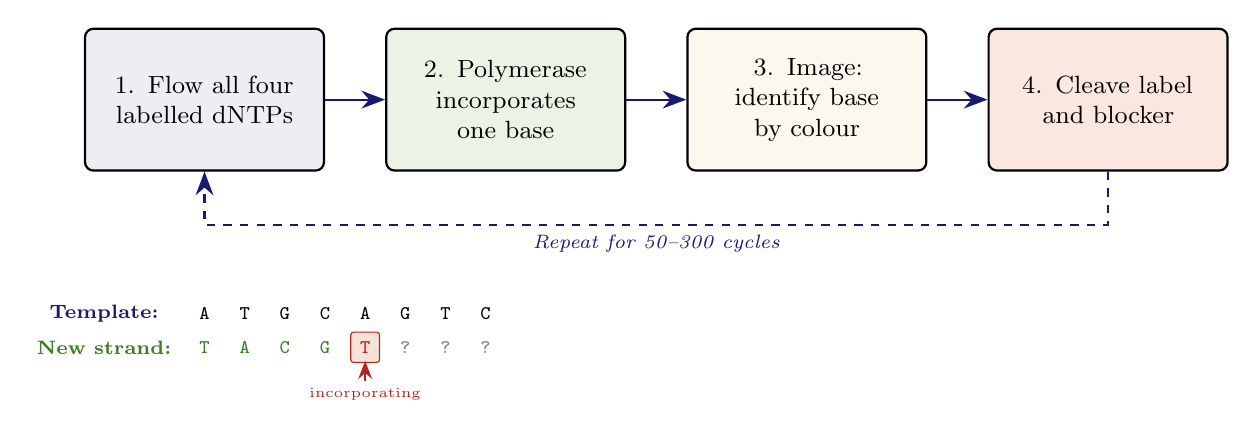
\begin{tikzpicture}[
  scale=0.85,
  every node/.style={font=\small},
  boxstep/.style={draw, rounded corners=3pt, thick, minimum width=3cm, minimum height=1.8cm, align=center, text width=2.8cm},
  arrow/.style={-{Stealth[length=3mm]}, thick, MidnightBlue}
]
  % Step 1
  \node[boxstep, fill=MidnightBlue!8] (s1) at (0,0) {1. Flow all four\\labelled dNTPs};

  % Step 2
  \node[boxstep, fill=OliveGreen!8] (s2) at (4.5,0) {2. Polymerase\\incorporates\\one base};

  % Step 3
  \node[boxstep, fill=Goldenrod!8] (s3) at (9,0) {3. Image:\\identify base\\by colour};

  % Step 4
  \node[boxstep, fill=BrickRed!8] (s4) at (13.5,0) {4. Cleave label\\and blocker};

  % Arrows
  \draw[arrow] (s1) -- (s2);
  \draw[arrow] (s2) -- (s3);
  \draw[arrow] (s3) -- (s4);

  % Cycle arrow back
  \draw[arrow, dashed] (s4.south) -- ++(0,-0.8) -| node[below, pos=0.25, font=\scriptsize\itshape] {Repeat for 50--300 cycles} (s1.south);

  % Template strand illustration below steps
  \begin{scope}[yshift=-3.2cm]
    % Template
    \node[font=\scriptsize\bfseries, MidnightBlue] at (-1.5,0) {Template:};
    \foreach \x/\base in {0/A, 0.6/T, 1.2/G, 1.8/C, 2.4/A, 3.0/G, 3.6/T, 4.2/C} {
      \node[font=\scriptsize\ttfamily] at (\x,0) {\base};
    }

    % Growing strand
    \node[font=\scriptsize\bfseries, OliveGreen] at (-1.5,-0.5) {New strand:};
    \foreach \x/\base in {0/T, 0.6/A, 1.2/C, 1.8/G} {
      \node[font=\scriptsize\ttfamily, OliveGreen] at (\x,-0.5) {\base};
    }
    % Current incorporation
    \node[font=\scriptsize\ttfamily, BrickRed, draw, rounded corners=1pt, fill=BrickRed!10] at (2.4,-0.5) {T};
    \draw[-{Stealth}, BrickRed, thick] (2.4,-1.0) -- (2.4,-0.7);
    \node[font=\tiny, BrickRed] at (2.4,-1.2) {incorporating};

    % Remaining template
    \foreach \x/\base in {3.0/?, 3.6/?, 4.2/?} {
      \node[font=\scriptsize\ttfamily, gray] at (\x,-0.5) {\base};
    }
  \end{scope}

\end{tikzpicture}
\caption[Sequencing by synthesis (SBS) principle.]{The cycle of Illumina sequencing by synthesis (SBS). In each cycle, all four fluorescently labelled reversible terminators are presented to the growing strand. DNA polymerase incorporates one complementary base, which is identified by its fluorescent colour after imaging. The fluorescent label and 3$'${} blocking group are then removed, and the cycle repeats.}
\label{fig:seqprinciples:sbs}
\end{figure}

\subsection{Cluster Generation}
\label{subsec:seqprinciples:clusters}

Before sequencing can begin on Illumina platforms, individual library fragments must be amplified into clusters of identical copies to generate a detectable fluorescent signal. This is accomplished through \textbf{bridge amplification} (also called \textbf{cluster generation}) on the surface of a \textbf{flow cell}:

\begin{enumerate}[itemsep=2pt]
  \item Library fragments are denatured (single-stranded) and flow across the flow cell, which is coated with short oligonucleotides complementary to the adapter sequences.
  \item Fragments hybridise to the surface oligos and are copied by a polymerase.
  \item The original template is washed away; the new copy bends over and hybridises to an adjacent surface oligo (forming a ``bridge'').
  \item The bridge is extended by polymerase, creating a double-stranded bridge.
  \item The bridge is denatured, yielding two single-stranded copies tethered to the surface.
  \item This process repeats through many cycles, producing a tight cluster of approximately 1,000 identical copies of the original fragment.
\end{enumerate}

Each cluster produces a coherent fluorescent signal during sequencing, effectively amplifying the signal from a single molecule.

\begin{warningbox}
Cluster generation introduces a potential source of error: if two different library fragments land too close together on the flow cell and their clusters overlap, the result is a ``mixed'' cluster that produces ambiguous base calls. More sophisticated patterned flow cells (used in NovaSeq and newer platforms) mitigate this by arranging cluster positions in a regular grid, but mixed clusters remain a consideration in data quality.
\end{warningbox}


% ============================================================
\section{Sequencing by Ligation}
\label{sec:seqprinciples:sbl}

\textbf{Sequencing by ligation} is an alternative approach in which DNA sequence is determined by the successive ligation (joining) of fluorescently labelled oligonucleotide probes to a primer hybridised to the template. Rather than using a polymerase to add single nucleotides, a ligase is used to join short probes whose identity encodes the sequence of the template.

This approach was used by the \textbf{SOLiD} (Sequencing by Oligonucleotide Ligation and Detection) platform from Applied Biosystems (later Life Technologies, now Thermo Fisher). In SOLiD sequencing:

\begin{enumerate}[itemsep=2pt]
  \item A universal primer hybridises to the adapter sequence adjacent to the unknown template.
  \item A pool of fluorescently labelled 8-mer oligonucleotide probes is added. Each probe interrogates two bases at a time (the first two bases of the probe encode the fluorescent colour in a two-base encoding scheme).
  \item DNA ligase joins the probe to the primer if it matches the template.
  \item The fluorescent signal is recorded, identifying the dinucleotide.
  \item The fluorescent label is cleaved, and the cycle repeats with the next probe.
  \item After several rounds, the extended strand is stripped, and the process restarts with a primer offset by one base, eventually covering every position.
\end{enumerate}

The two-base encoding scheme in SOLiD meant that each base was interrogated twice, providing inherent error correction. However, the short read lengths (50--75\basepair{}), relatively slow throughput, and complex data analysis led to SOLiD being largely superseded by Illumina platforms. The sequencing-by-ligation concept is primarily of historical interest, though elements of it persist in some specialised applications.


% ============================================================
\section{Nanopore Sequencing}
\label{sec:seqprinciples:nanopore}

\textbf{Nanopore sequencing}, commercialised by \acrfull{ONT}, takes a fundamentally different approach: instead of synthesising a new strand or ligating probes, it reads DNA (or RNA) directly by threading a single molecule through a tiny protein pore and measuring the resulting changes in electrical current.

\subsection{The Principle}
\label{subsec:seqprinciples:nanopore-principle}

The core of a nanopore sequencer is a biological \textbf{nanopore}---a protein channel (currently a modified version of the CsgG protein) embedded in an electrically resistant polymer membrane. A voltage is applied across the membrane, driving a constant ionic current through the pore. When a strand of DNA passes through the pore:

\begin{enumerate}[itemsep=2pt]
  \item A \textbf{motor protein} (a helicase) at the top of the pore controls the translocation speed, feeding the DNA strand through the pore one nucleotide at a time.
  \item As each nucleotide (or, more precisely, a k-mer of approximately 5--6 nucleotides) passes through the constriction zone of the pore, it partially blocks the ionic current.
  \item The degree of current disruption depends on the identity and combination of bases in the constriction zone.
  \item A sensitive amplifier measures the current in real time, producing a \textbf{signal trace} (a ``squiggle'') of current vs.\ time.
  \item A computational algorithm (\textbf{basecaller}, typically a neural network) converts the raw signal into a nucleotide sequence.
\end{enumerate}

% TikZ: Nanopore sequencing principle
\begin{figure}[htbp]
\centering
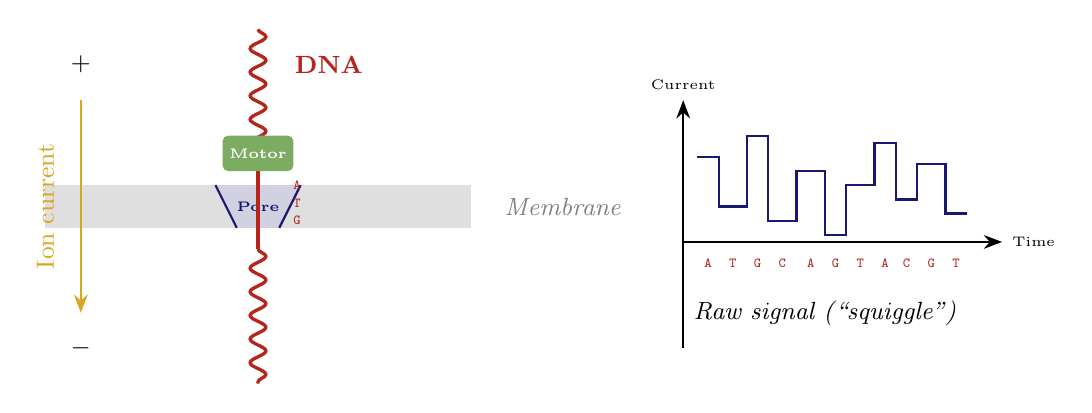
\begin{tikzpicture}[scale=0.9]
  % Membrane
  \fill[gray!25] (-3,-0.3) rectangle (3,0.3);
  \node[font=\small\itshape, gray] at (4.3,0) {Membrane};

  % Pore (hourglass shape)
  \fill[MidnightBlue!20] (-0.6,0.3) -- (-0.3,-0.3) -- (0.3,-0.3) -- (0.6,0.3) -- cycle;
  \draw[thick, MidnightBlue] (-0.6,0.3) -- (-0.3,-0.3);
  \draw[thick, MidnightBlue] (0.6,0.3) -- (0.3,-0.3);
  \node[font=\tiny\bfseries, MidnightBlue] at (0,0) {Pore};

  % DNA strand going through
  \draw[very thick, BrickRed, decorate, decoration={snake, amplitude=1mm, segment length=3mm}]
    (0,2.5) -- (0,0.6);
  \draw[very thick, BrickRed] (0,0.6) -- (0,-0.6);
  \draw[very thick, BrickRed, decorate, decoration={snake, amplitude=1mm, segment length=3mm}]
    (0,-0.6) -- (0,-2.5);

  % DNA label
  \node[font=\small\bfseries, BrickRed] at (1.0,2.0) {DNA};

  % Motor protein
  \fill[OliveGreen!60, rounded corners=2pt] (-0.5,0.5) rectangle (0.5,1.0);
  \node[font=\tiny\bfseries, white] at (0,0.75) {Motor};

  % Bases passing through constriction
  \foreach \y/\base in {0.3/A, 0.05/T, -0.2/G} {
    \node[font=\tiny\bfseries\ttfamily, BrickRed] at (0.55,\y) {\base};
  }

  % Current flow arrows
  \draw[-{Stealth}, thick, Goldenrod] (-2.5,1.5) -- (-2.5,-1.5);
  \node[font=\small, Goldenrod, rotate=90] at (-3.0,0) {Ion current};

  % Voltage labels
  \node[font=\small] at (-2.5,2.0) {$+$};
  \node[font=\small] at (-2.5,-2.0) {$-$};

  % Signal trace (right side)
  \begin{scope}[xshift=6cm, yshift=-0.5cm]
    \draw[thick, -{Stealth}] (0,0) -- (4.5,0) node[right, font=\tiny] {Time};
    \draw[thick, -{Stealth}] (0,-1.5) -- (0,2) node[above, font=\tiny] {Current};

    % Squiggle signal
    \draw[thick, MidnightBlue]
      (0.2,1.2) -- (0.5,1.2) -- (0.5,0.5) -- (0.9,0.5) -- (0.9,1.5) -- (1.2,1.5)
      -- (1.2,0.3) -- (1.6,0.3) -- (1.6,1.0) -- (2.0,1.0) -- (2.0,0.1) -- (2.3,0.1)
      -- (2.3,0.8) -- (2.7,0.8) -- (2.7,1.4) -- (3.0,1.4) -- (3.0,0.6) -- (3.3,0.6)
      -- (3.3,1.1) -- (3.7,1.1) -- (3.7,0.4) -- (4.0,0.4);

    % Base labels below signal
    \node[font=\tiny\ttfamily, BrickRed] at (0.35,-0.3) {A};
    \node[font=\tiny\ttfamily, BrickRed] at (0.7,-0.3) {T};
    \node[font=\tiny\ttfamily, BrickRed] at (1.05,-0.3) {G};
    \node[font=\tiny\ttfamily, BrickRed] at (1.4,-0.3) {C};
    \node[font=\tiny\ttfamily, BrickRed] at (1.8,-0.3) {A};
    \node[font=\tiny\ttfamily, BrickRed] at (2.15,-0.3) {G};
    \node[font=\tiny\ttfamily, BrickRed] at (2.5,-0.3) {T};
    \node[font=\tiny\ttfamily, BrickRed] at (2.85,-0.3) {A};
    \node[font=\tiny\ttfamily, BrickRed] at (3.15,-0.3) {C};
    \node[font=\tiny\ttfamily, BrickRed] at (3.5,-0.3) {G};
    \node[font=\tiny\ttfamily, BrickRed] at (3.85,-0.3) {T};

    \node[font=\small\itshape] at (2.0,-1.0) {Raw signal (``squiggle'')};
  \end{scope}

\end{tikzpicture}
\caption[Nanopore sequencing principle.]{The principle of nanopore sequencing. A single strand of DNA is threaded through a protein nanopore embedded in a membrane. A motor protein controls the translocation speed. As bases pass through the pore's constriction, they modulate the ionic current. The resulting signal trace (``squiggle'') is decoded by a neural network basecaller to determine the DNA sequence.}
\label{fig:seqprinciples:nanopore}
\end{figure}

\subsection{Key Features of Nanopore Sequencing}
\label{subsec:seqprinciples:nanopore-features}

\begin{itemize}[itemsep=3pt]
  \item \textbf{Ultra-long reads:} There is no theoretical upper limit to read length. Reads exceeding 4\megabase{} have been demonstrated. In routine practice, reads of 10--100\kilobase{} are common with appropriate library preparation.
  \item \textbf{Direct detection of base modifications:} Because the raw signal is sensitive to chemical modifications, nanopore sequencing can detect 5-methylcytosine (5mC), 5-hydroxymethylcytosine (5hmC), N$^6$-methyladenosine (m$^6$A), and other modifications directly, without bisulfite conversion or antibody enrichment.
  \item \textbf{Direct RNA sequencing:} \acrshort{ONT} offers a direct RNA sequencing protocol that threads native RNA molecules through the pore, avoiding reverse transcription and \acrshort{PCR} amplification entirely.
  \item \textbf{Real-time data:} Data is generated and can be analysed as the sequencing run progresses, enabling applications like adaptive sampling (selectively sequencing or rejecting individual molecules in real time).
  \item \textbf{Portability:} The MinION weighs about 100 grams and connects via USB. It has been used in the field for pathogen surveillance, in space on the ISS, and in Antarctic research stations.
  \item \textbf{Higher error rate:} Raw single-pass accuracy is approximately 92--98\% (depending on pore chemistry and basecaller version), with errors primarily being insertions and deletions (indels), especially in homopolymer regions (runs of the same base). Consensus accuracy from multiple reads of the same region can exceed 99.9\%.
\end{itemize}


% ============================================================
\section{Single-Molecule Real-Time (SMRT) Sequencing}
\label{sec:seqprinciples:smrt}

\textbf{\Acrfull{SMRTseq}}, developed by \acrfull{PacBio}, reads individual DNA molecules in real time by watching a single polymerase as it synthesises a complementary strand.

\subsection{The Principle}
\label{subsec:seqprinciples:smrt-principle}

SMRT sequencing uses a \textbf{zero-mode waveguide (ZMW)}---a tiny well (approximately 70\,nm in diameter and 100\,nm deep) fabricated in a metal film on a glass substrate. A single DNA polymerase molecule is immobilised at the bottom of each ZMW, and a single circular DNA template molecule (a \textbf{SMRTbell}) is bound to the polymerase.

\begin{enumerate}[itemsep=2pt]
  \item All four fluorescently labelled nucleotides (each with a distinct colour) are present in solution simultaneously.
  \item When the polymerase binds and incorporates a nucleotide, the fluorophore is held in the detection volume of the ZMW long enough to emit a characteristic pulse of light.
  \item The fluorophore is cleaved from the nucleotide as part of the incorporation process (it is attached to the phosphate group, which is released as pyrophosphate).
  \item The sequence of fluorescent pulses over time reveals the sequence of incorporated bases.
\end{enumerate}

The ZMW is so small that even though the solution is filled with fluorescent nucleotides, only nucleotides within the tiny detection volume at the bottom of the well contribute significantly to the signal. This allows detection of single-molecule incorporation events against the background.

% TikZ: SMRT sequencing principle
\begin{figure}[htbp]
\centering
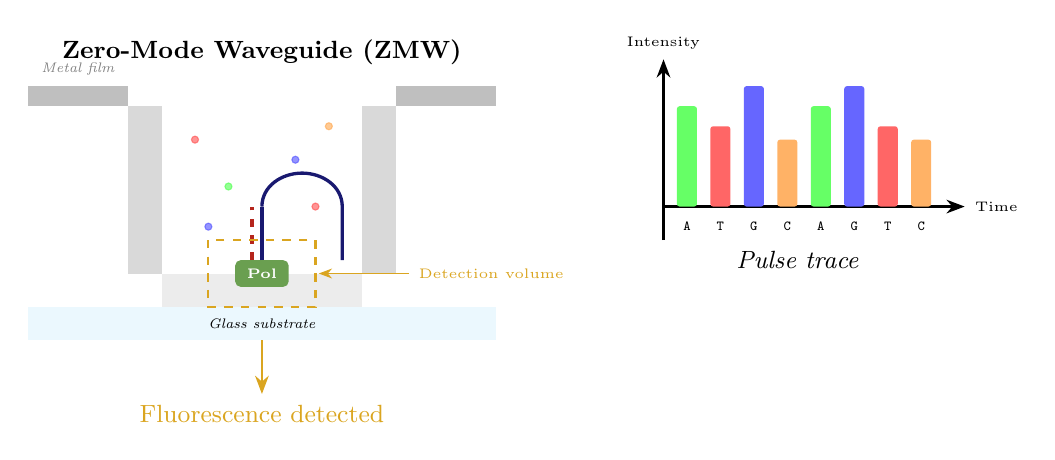
\begin{tikzpicture}[scale=0.85]
  % ZMW well
  \fill[gray!30] (-2,0) rectangle (-1.5,-2.5);
  \fill[gray!30] (1.5,0) rectangle (2,-2.5);
  \fill[gray!15] (-1.5,-2.5) rectangle (1.5,-3.0);

  % Metal film
  \fill[gray!50] (-3.5,0) rectangle (-2,0.3);
  \fill[gray!50] (2,0) rectangle (3.5,0.3);
  \node[font=\tiny\itshape, gray] at (-2.75,0.55) {Metal film};

  % Glass substrate
  \fill[cyan!8] (-3.5,-3.0) rectangle (3.5,-3.5);
  \node[font=\tiny\itshape] at (0,-3.25) {Glass substrate};

  % Polymerase at bottom
  \fill[OliveGreen!70, rounded corners=2pt] (-0.4,-2.7) rectangle (0.4,-2.3);
  \node[font=\tiny\bfseries, white] at (0,-2.5) {Pol};

  % SMRTbell template (circular)
  \draw[very thick, MidnightBlue] (0,-2.3) -- (0,-1.5);
  \draw[very thick, MidnightBlue] (0,-1.5) to[out=90,in=180] (0.6,-1.0) to[out=0,in=90] (1.2,-1.5) -- (1.2,-2.3);
  \draw[very thick, BrickRed, dashed] (-0.15,-2.3) -- (-0.15,-1.5);

  % Fluorescent nucleotides in solution
  \foreach \x/\y/\col in {-1.0/-0.5/red, 0.5/-0.8/blue, -0.5/-1.2/green, 1.0/-0.3/orange, -0.8/-1.8/blue, 0.8/-1.5/red} {
    \filldraw[\col!70, opacity=0.6] (\x,\y) circle (1.5pt);
  }

  % Detection volume (highlighted zone)
  \draw[Goldenrod, thick, dashed] (-0.8,-2.0) rectangle (0.8,-3.0);
  \node[font=\tiny, Goldenrod, anchor=west] at (2.2,-2.5) {Detection volume};
  \draw[-{Stealth}, Goldenrod, thin] (2.2,-2.5) -- (0.85,-2.5);

  % Light emission arrow
  \draw[-{Stealth}, thick, Goldenrod] (0,-3.5) -- (0,-4.3);
  \node[font=\small, Goldenrod] at (0,-4.6) {Fluorescence detected};

  % ZMW label
  \node[font=\small\bfseries] at (0,0.8) {Zero-Mode Waveguide (ZMW)};

  % Pulse trace
  \begin{scope}[xshift=6cm, yshift=-1.5cm]
    \draw[thick, -{Stealth}] (0,0) -- (4.5,0) node[right, font=\tiny] {Time};
    \draw[thick, -{Stealth}] (0,-0.5) -- (0,2.2) node[above, font=\tiny] {Intensity};

    % Pulses of different colours
    \fill[green!60, rounded corners=1pt] (0.2,0) rectangle (0.5,1.5);
    \fill[red!60, rounded corners=1pt] (0.7,0) rectangle (1.0,1.2);
    \fill[blue!60, rounded corners=1pt] (1.2,0) rectangle (1.5,1.8);
    \fill[orange!60, rounded corners=1pt] (1.7,0) rectangle (2.0,1.0);
    \fill[green!60, rounded corners=1pt] (2.2,0) rectangle (2.5,1.5);
    \fill[blue!60, rounded corners=1pt] (2.7,0) rectangle (3.0,1.8);
    \fill[red!60, rounded corners=1pt] (3.2,0) rectangle (3.5,1.2);
    \fill[orange!60, rounded corners=1pt] (3.7,0) rectangle (4.0,1.0);

    % Base labels
    \foreach \x/\base in {0.35/A, 0.85/T, 1.35/G, 1.85/C, 2.35/A, 2.85/G, 3.35/T, 3.85/C} {
      \node[font=\tiny\ttfamily\bfseries] at (\x,-0.3) {\base};
    }
    \node[font=\small\itshape] at (2.0,-0.8) {Pulse trace};
  \end{scope}

\end{tikzpicture}
\caption[SMRT sequencing principle.]{The principle of PacBio SMRT sequencing. A single DNA polymerase is immobilised at the bottom of a zero-mode waveguide (ZMW). Fluorescently labelled nucleotides are incorporated one at a time; each incorporation produces a characteristic pulse of light whose colour identifies the base. The ZMW's tiny detection volume ensures that only nucleotides being incorporated contribute to the signal.}
\label{fig:seqprinciples:smrt}
\end{figure}

\subsection{SMRTbell Templates and HiFi Reads}
\label{subsec:seqprinciples:smrtbell}

A key innovation in PacBio sequencing is the \textbf{SMRTbell} library format. The double-stranded DNA insert is flanked by hairpin adapters, creating a single-stranded circular molecule. The polymerase can read around the circle multiple times (called \textbf{subreads} or \textbf{passes}), generating redundant coverage of the same molecule.

\begin{itemize}[itemsep=2pt]
  \item \textbf{Continuous long reads (CLR):} The polymerase reads the SMRTbell once or a few times. CLR reads can be very long (>50\kilobase{}) but have a raw single-pass error rate of approximately 10--15\% (mostly insertion errors).
  \item \textbf{HiFi reads (CCS):} For shorter inserts (typically 10--25\kilobase{}), the polymerase makes many passes around the SMRTbell. The multiple passes are computationally combined via \textbf{circular consensus sequencing (CCS)} to produce \textbf{HiFi reads} with accuracy exceeding 99.9\% (Q30+). HiFi reads combine the advantages of long reads (resolving repeats, structural variants, and full-length transcripts) with the accuracy of short reads.
\end{itemize}

\begin{keyconcept}[title={HiFi Reads: The Best of Both Worlds}]
PacBio HiFi reads (typically 10--25\kilobase{}, >Q20 accuracy) represent a significant advance: they are long enough to span most repetitive elements and structural variants, yet accurate enough for confident variant calling and haplotype phasing. HiFi sequencing has become a cornerstone technology for high-quality genome assembly and comprehensive variant detection.
\end{keyconcept}


% ============================================================
\section{Key Sequencing Metrics}
\label{sec:seqprinciples:metrics}

To evaluate and compare sequencing technologies and to plan experiments, several key metrics are used.

\subsection{Read Length}
\label{subsec:seqprinciples:read-length}

The \textbf{read length} is the number of bases sequenced per fragment (per read). It varies dramatically across platforms:

\begin{itemize}[itemsep=2pt]
  \item \textbf{Illumina:} Typically 50--300\basepair{} (most commonly 150\basepair{} paired-end).
  \item \textbf{PacBio HiFi:} Typically 10--25\kilobase{}.
  \item \textbf{PacBio CLR:} Up to $>$100\kilobase{}.
  \item \textbf{Oxford Nanopore:} Routinely 10--100\kilobase{}; records exceed 4\megabase{}.
\end{itemize}

Longer reads are advantageous for resolving repetitive regions, detecting structural variants, phasing haplotypes, and assembling genomes. Shorter reads are typically cheaper per base and have lower per-base error rates.

\subsection{Throughput}
\label{subsec:seqprinciples:throughput}

\textbf{Throughput} is the total amount of sequence data generated per run, usually expressed in gigabases (\gigabase{}). A run must be defined carefully: Illumina reports output by flow-cell type and read configuration, PacBio may report yield per SMRT Cell and per multi-cell instrument run, and ONT flow cells can be stopped at a user-selected time. As verified on 1 September 2026, an Illumina NovaSeq X Plus dual-25B run is specified at up to approximately 16~Tb, whereas a MinION/GridION flow cell has a theoretical maximum near 50~Gb. These are vendor specifications rather than guaranteed yields; library type and run performance affect realized output.

\subsection{Accuracy and Error Profiles}
\label{subsec:seqprinciples:accuracy}

\textbf{Accuracy} describes how often the sequencer correctly identifies the base. Different technologies exhibit different \textbf{error profiles}:

\begin{itemize}[itemsep=2pt]
  \item \textbf{Illumina (SBS):} Very high per-base accuracy ($>$99.9\%). Dominant error type is \textbf{substitution errors} (one base called instead of another). Errors increase toward the end of reads due to phasing effects and signal decay.
  \item \textbf{PacBio (SMRT):} Raw single-pass accuracy $\sim$85--90\%, but HiFi consensus accuracy exceeds 99.9\%. Dominant error type is \textbf{insertion errors}.
  \item \textbf{Oxford Nanopore:} Raw single-pass accuracy $\sim$92--98\% (improving with newer pore chemistries and basecallers). Dominant error types are \textbf{insertions and deletions (indels)}, particularly in homopolymer regions (e.g., AAAAAA).
\end{itemize}

\begin{warningbox}
The error \textit{type} matters as much as the error \textit{rate}. Substitution errors (Illumina) are relatively easy to correct computationally because they rarely occur at the same position in multiple reads. Systematic indel errors (nanopore, PacBio CLR), especially in homopolymers, are more challenging because they can be consistent across reads from the same region.
\end{warningbox}


% ============================================================
\section{Paired-End vs.\ Single-End Reads}
\label{sec:seqprinciples:paired-end}

When sequencing a library on Illumina platforms, you can choose to sequence from one end of each fragment (\textbf{single-end} reads) or from both ends (\textbf{paired-end} reads).

\begin{description}[style=nextline, itemsep=3pt]
  \item[Single-end (SE) sequencing] Each fragment is sequenced from one end only, producing one read per fragment. Example: 1$\times$75\basepair{} (one read of 75 bases).

  \item[Paired-end (PE) sequencing] Each fragment is sequenced from both ends, producing two reads per fragment. The two reads are from opposite ends of the same fragment and are in opposite orientations. Example: 2$\times$150\basepair{} (two reads of 150 bases each, from opposite ends).
\end{description}

Paired-end sequencing provides several advantages:
\begin{itemize}[itemsep=2pt]
  \item \textbf{Improved alignment:} Both reads from a pair should map to locations separated by the expected insert size, providing a constraint that improves mapping accuracy, especially in repetitive regions.
  \item \textbf{Structural variant detection:} Abnormal spacing or orientation of paired reads indicates insertions, deletions, inversions, or translocations.
  \item \textbf{Improved assembly:} Paired reads provide long-range connectivity information that helps bridge gaps in genome assembly.
  \item \textbf{Insert size estimation:} The distance between paired reads provides the fragment size distribution, which is a useful quality metric.
\end{itemize}

\begin{tipbox}
For most applications (WGS, RNA-seq, ATAC-seq, ChIP-seq), paired-end 150\basepair{} (2$\times$150) sequencing is the standard choice on Illumina platforms. Single-end sequencing may be cost-effective for some applications (e.g., miRNA-seq, where fragments are short) or when the primary goal is counting (e.g., some ChIP-seq experiments).
\end{tipbox}


% ============================================================
\section{Read Depth and Coverage}
\label{sec:seqprinciples:coverage}

Two of the most important concepts in experimental design are \textbf{read depth} and \textbf{coverage}.

\subsection{Definitions}
\label{subsec:seqprinciples:coverage-def}

\begin{description}[style=nextline, itemsep=3pt]
  \item[Sequencing depth (read depth)] The total number of reads generated in a sequencing experiment. Sometimes expressed as the total number of base pairs generated.

  \item[Coverage (fold coverage, denoted $\times$)] The average number of times each base in the target region (e.g., the genome) is read. For example, 30$\times$ coverage means that, on average, each position in the genome is covered by 30 independent reads.
\end{description}

Coverage can be calculated as:

\begin{equation}
\text{Coverage} = \frac{N \times L}{G}
\label{eq:seqprinciples:coverage}
\end{equation}

where $N$ is the number of reads, $L$ is the read length (in base pairs), and $G$ is the genome size (in base pairs).

\begin{keyconcept}[title={Calculating Coverage}]
For a human genome ($G \approx 3.2 \times 10^9$\basepair{}) sequenced with 800 million paired-end 150\basepair{} reads ($N = 800 \times 10^6 \times 2 = 1.6 \times 10^9$ reads total, $L = 150$\basepair{}):
\[
\text{Coverage} = \frac{1.6 \times 10^9 \times 150}{3.2 \times 10^9} = \frac{2.4 \times 10^{11}}{3.2 \times 10^9} = 75\times
\]
This is a rough estimate. Actual coverage will be somewhat lower due to PCR duplicates, low-quality reads, and reads mapping to multiple locations.
\end{keyconcept}

\subsection{Why Coverage Matters}
\label{subsec:seqprinciples:coverage-importance}

Coverage is critical because sequencing is fundamentally a \textbf{sampling process}: each read represents a random sample from the pool of library fragments. Higher coverage means more samples, which translates to:

\begin{itemize}[itemsep=2pt]
  \item \textbf{More confident base calls:} At a heterozygous SNP position (where the individual has one copy of each allele), you need enough reads to observe both alleles reliably. At 30$\times$ coverage, a heterozygous site will have, on average, $\sim$15 reads supporting each allele, providing high confidence.
  \item \textbf{Better structural variant detection:} SVs require multiple discordant or split reads to be detected with confidence.
  \item \textbf{More uniform representation:} Higher coverage helps compensate for biases in library preparation that cause some regions to be over-represented and others under-represented.
\end{itemize}

Typical coverage requirements vary by application:

\begin{table}[htbp]
\centering
\caption{Typical coverage requirements for common sequencing applications.}
\label{tab:seqprinciples:coverage-requirements}
\small
\begin{tabularx}{\textwidth}{>{\bfseries}l X r}
\toprule
\textbf{Application} & \textbf{Purpose} & \textbf{Typical Coverage} \\
\midrule
WGS (germline variants) & SNV and indel detection & 30--60$\times$ \\
WGS (somatic variants) & Tumour mutation detection & 60--100$\times$ \\
WES (exome) & Coding region variant detection & 100--200$\times$ \\
RNA-seq (bulk) & Gene expression quantification & 20--50M reads/sample \\
scRNA-seq & Single-cell expression profiling & 20,000--50,000 reads/cell \\
ChIP-seq & Protein--DNA binding & 20--40M reads/sample \\
ATAC-seq & Chromatin accessibility & 50--75M reads/sample \\
WGBS & DNA methylation & 10--30$\times$ \\
Hi-C & 3D genome architecture & 200M--1B read pairs \\
\bottomrule
\end{tabularx}
\end{table}

\begin{warningbox}
Coverage is an \textit{average}. Due to biases (GC content, mappability, library complexity), some regions may have far more or far less coverage than the average. For clinical applications, minimum coverage thresholds at specific genomic positions (e.g., $\geq$20$\times$ at $\geq$95\% of target bases) are often more informative than average coverage alone.
\end{warningbox}


\subsection{The Lander--Waterman Model of Coverage}
\label{subsec:seqprinciples:lander-waterman}

The relationship between average coverage and the fraction of the genome covered by at least one read is formalised by the \textbf{Lander--Waterman model} (1988). If we assume that reads are distributed uniformly and independently (a Poisson process), then the probability that a given base is \textit{not} covered by any read is:

\begin{equation}
P(\text{uncovered}) = e^{-c}
\label{eq:seqprinciples:lander-waterman}
\end{equation}

where $c = NL/G$ is the average coverage depth. Therefore, the fraction of the genome covered by at least one read is:

\begin{equation}
P(\text{covered}) = 1 - e^{-c}
\label{eq:seqprinciples:genome-coverage}
\end{equation}

More generally, the probability that a position is covered by exactly $k$ reads follows a Poisson distribution:

\begin{equation}
P(X = k) = \frac{c^k \, e^{-c}}{k!}
\label{eq:seqprinciples:poisson-coverage}
\end{equation}

\begin{keyconcept}[title={Coverage Thresholds from the Lander--Waterman Model}]
At 30$\times$ average coverage, the Lander--Waterman model predicts that $1 - e^{-30} \approx 99.9999999\%$ of the genome is covered by at least one read. However, the fraction covered at $\geq$20$\times$ (important for confident variant calling) is:
\[
P(X \geq 20 \mid c=30) = 1 - \sum_{k=0}^{19} \frac{30^k e^{-30}}{k!} \approx 98.5\%
\]
This means roughly 1.5\% of the genome may fall below 20$\times$ even at 30$\times$ average coverage---a non-trivial fraction for clinical applications.
\end{keyconcept}

The Lander--Waterman model assumes \textbf{uniform random sampling}, which is an idealisation. In practice, coverage is not Poisson-distributed due to:

\begin{itemize}[itemsep=2pt]
  \item \textbf{GC bias:} Regions with extreme GC content (very high or very low) are under-represented in most library preparations, particularly those involving \acrshort{PCR} amplification.
  \item \textbf{Mappability:} Repetitive regions where reads cannot be uniquely placed effectively have zero usable coverage.
  \item \textbf{Library preparation biases:} Fragmentation, adapter ligation, and amplification each introduce systematic deviations from uniformity.
\end{itemize}

A more realistic model replaces the Poisson with a \textbf{negative binomial} distribution, which adds a dispersion parameter $r$ to account for overdispersion:

\begin{equation}
P(X = k) = \binom{k + r - 1}{k} \left(\frac{r}{r + c}\right)^r \left(\frac{c}{r + c}\right)^k
\label{eq:seqprinciples:nb-coverage}
\end{equation}

where the variance is $\text{Var}(X) = c + c^2/r$. As $r \to \infty$, the negative binomial converges to the Poisson.


\subsection{Adapter Ligation Efficiency}
\label{subsec:seqprinciples:ligation-efficiency}

A critical but often overlooked parameter in library preparation is the \textbf{adapter ligation efficiency}---the fraction of DNA fragments that successfully receive adapters on both ends and are therefore sequenceable. Fragments with adapters on only one end (or no adapters) are invisible to the sequencing instrument.

Ligation efficiency depends on several factors:

\begin{itemize}[itemsep=2pt]
  \item \textbf{End quality:} Blunt-ended or A-tailed fragments ligate more efficiently than fragments with damaged or ragged ends. Enzymatic end repair is a standard step to maximise efficiency.
  \item \textbf{Adapter:insert molar ratio:} Typically 10:1 to 100:1 excess of adapter molecules to fragment ends, ensuring that adapters are not limiting.
  \item \textbf{Ligase and buffer conditions:} T4 DNA ligase at 20$\,^\circ$C for 10--30 minutes is standard. Lower temperatures favour ligation fidelity; longer incubations increase efficiency.
  \item \textbf{Fragment size:} Very short fragments ($<$100\basepair{}) may ligate to adapters less efficiently due to steric constraints, while very long fragments ($>$20\kilobase{}) may suffer from shearing during handling.
\end{itemize}

If we denote the probability of successful adapter ligation to one end as $p$, then the probability that a fragment receives adapters on both ends (and is therefore sequenceable) is $p^2$. For typical ligation efficiencies of $p = 0.7$--$0.9$, this yields:

\begin{table}[htbp]
\centering
\caption{Effect of single-end ligation efficiency on overall library yield.}
\label{tab:seqprinciples:ligation-efficiency}
\small
\begin{tabular}{ccc}
\toprule
\textbf{Single-end efficiency ($p$)} & \textbf{Both-ends efficiency ($p^2$)} & \textbf{Effective library yield} \\
\midrule
0.70 & 0.49 & 49\% of input fragments \\
0.80 & 0.64 & 64\% of input fragments \\
0.90 & 0.81 & 81\% of input fragments \\
0.95 & 0.90 & 90\% of input fragments \\
\bottomrule
\end{tabular}
\end{table}

\begin{tipbox}
Ligation efficiency is one reason why the recommended minimum input for many library prep kits is 100--500 ng of DNA. Starting with less material means fewer fragments, and if ligation efficiency is suboptimal, the resulting library may have low complexity. For low-input protocols ($<$10 ng), specialised kits with optimised ligation chemistries or tagmentation-based approaches (which bypass traditional ligation) are preferred.
\end{tipbox}


% ============================================================
\section{Multiplexing and Barcoding}
\label{sec:seqprinciples:multiplexing}

Modern sequencing instruments generate far more data than is needed for a single sample in many applications. \textbf{Multiplexing} (also called \textbf{pooling}) is the practice of combining multiple samples on a single sequencing run, using short DNA \textbf{barcodes} (also called \textbf{indexes} or \textbf{index sequences}) to identify which reads came from which sample.

\subsection{How Indexing Works}
\label{subsec:seqprinciples:indexing}

During library preparation, each sample's fragments receive a unique barcode sequence incorporated into the adapter. Illumina uses \textbf{dual indexing}: two independent index sequences (i7 and i5) of 8--10\basepair{} each are incorporated into the adapter, one on each end of the fragment. After sequencing, an additional ``index read'' determines the barcode sequence, and reads are computationally sorted (\textbf{demultiplexed}) by barcode into sample-specific files.

\subsection{Benefits of Multiplexing}
\label{subsec:seqprinciples:multiplexing-benefits}

\begin{itemize}[itemsep=2pt]
  \item \textbf{Cost efficiency:} The sequencing run cost is shared among multiple samples. For example, if a NovaSeq S4 flow cell generates $\sim$10 billion read pairs, and your RNA-seq experiment requires 30 million reads per sample, you can multiplex over 300 samples on a single flow cell.
  \item \textbf{Experimental design:} By balancing experimental conditions across lanes and flow cells, multiplexing reduces batch effects.
  \item \textbf{Flexibility:} Different amounts of data can be allocated to different samples by adjusting the ratio of library input.
\end{itemize}

\begin{warningbox}[title={Index Hopping}]
On some Illumina platforms with patterned flow cells (e.g., NovaSeq 6000 with the v1.0 reagent kit), a phenomenon called \textbf{index hopping} (or \textbf{index switching}) can occur: free adapter molecules from one sample can recombine with clusters from another sample during the exclusion amplification step, leading to incorrect sample assignment of a small percentage of reads (typically 0.1--2\%). Using \textbf{unique dual indexes (UDIs)}---where both the i7 and i5 indexes are unique to each sample---allows computational detection and removal of hopped reads. This problem has been significantly reduced in newer platforms and reagent kits.
\end{warningbox}


% ============================================================
\section{Quality Scores: Phred Scores and Q30}
\label{sec:seqprinciples:quality-scores}

Every base call produced by a sequencing instrument is accompanied by a \textbf{quality score} that estimates the probability that the base call is incorrect.

\subsection{Phred Quality Scores}
\label{subsec:seqprinciples:phred}

Quality scores follow the \textbf{Phred} scale, defined as:

\begin{equation}
Q = -10 \cdot \log_{10}(P_{\text{error}})
\label{eq:seqprinciples:phred}
\end{equation}

where $P_{\text{error}}$ is the estimated probability of an incorrect base call. Higher $Q$ values indicate higher confidence:

\begin{table}[htbp]
\centering
\caption{Phred quality scores and corresponding error probabilities.}
\label{tab:seqprinciples:phred-scores}
\small
\begin{tabular}{ccc}
\toprule
\textbf{Phred Score ($Q$)} & \textbf{Error Probability} & \textbf{Accuracy} \\
\midrule
10 & 1 in 10 (10\%) & 90\% \\
20 & 1 in 100 (1\%) & 99\% \\
30 & 1 in 1,000 (0.1\%) & 99.9\% \\
40 & 1 in 10,000 (0.01\%) & 99.99\% \\
50 & 1 in 100,000 (0.001\%) & 99.999\% \\
\bottomrule
\end{tabular}
\end{table}

\subsection{Q30 as a Benchmark}
\label{subsec:seqprinciples:q30}

\textbf{Q30} (a Phred score of 30, corresponding to 99.9\% accuracy) is widely used as a benchmark for sequencing quality. The ``percent of bases $\geq$ Q30'' is a standard metric reported by Illumina instruments. A typical Illumina run produces $>$85--90\% of bases at Q30 or above.


\subsection{From Phred to Neural Basecallers}
\label{subsec:seqprinciples:basecaller-math}

The original Phred program (developed for Sanger sequencing in the late 1990s) estimated base quality by examining features of the electropherogram trace---peak spacing, peak resolution, and signal-to-noise ratio---and mapping these features to empirically calibrated error probabilities. Modern basecallers use fundamentally different approaches.

\subsubsection{Neural Network Basecalling}

Contemporary basecallers---including Illumina's \software{DRAGEN}, \acrshort{ONT}'s \software{Dorado}, and PacBio's \software{DeepConsensus}---employ deep neural networks (typically recurrent or transformer architectures) that take raw signal data as input and produce base calls with associated quality scores.

For a neural basecaller, at each position the network outputs a vector of \textbf{logits} $\mathbf{z} = (z_A, z_C, z_G, z_T)$, which are transformed into probabilities via the \textbf{softmax} function:

\begin{equation}
P(b_i = k) = \frac{e^{z_k}}{\sum_{j \in \{A,C,G,T\}} e^{z_j}}, \quad k \in \{A,C,G,T\}
\label{eq:seqprinciples:softmax}
\end{equation}

The called base is the one with the highest probability: $\hat{b}_i = \arg\max_k P(b_i = k)$. The Phred quality score is then derived from the posterior probability:

\begin{equation}
Q_i = -10 \cdot \log_{10}\bigl(1 - P(b_i = \hat{b}_i)\bigr) = -10 \cdot \log_{10}(P_{\text{error},i})
\label{eq:seqprinciples:phred-from-softmax}
\end{equation}

\begin{warningbox}[title={Quality Score Calibration}]
Neural basecallers can produce \textbf{miscalibrated} quality scores: the predicted error probability may not match the actual observed error rate. For instance, a basecaller might assign Q30 to bases that empirically have Q25 accuracy. Well-calibrated quality scores are essential for downstream tools (e.g., variant callers that use quality scores as priors). Tools like \software{Dorado} include calibration steps, but users should always verify calibration using known reference samples.
\end{warningbox}


\subsubsection{Basecalling Models and Accuracy Trade-offs}

Modern nanopore basecallers offer multiple model tiers that trade speed for accuracy:

\begin{table}[htbp]
\centering
\caption[Basecaller model comparison.]{Comparison of \software{Dorado} basecalling model tiers for Oxford Nanopore R10.4.1 chemistry. Speed is approximate and depends on hardware.}
\label{tab:seqprinciples:basecaller-models}
\small
\begin{tabular}{lccl}
\toprule
\textbf{Model} & \textbf{Modal accuracy} & \textbf{Speed (samples/s)} & \textbf{Architecture} \\
\midrule
Fast & Q10--Q14 ($\sim$90--96\%) & $4 \times 10^6$ & Small CTC/CRF \\
HAC (high accuracy) & Q16--Q20 ($\sim$97--99\%) & $1 \times 10^6$ & Medium CRF \\
SUP (super accuracy) & Q20--Q25 ($\sim$99--99.7\%) & $3 \times 10^5$ & Large transformer \\
\bottomrule
\end{tabular}
\end{table}

The ``fast'' model is suitable for real-time applications (e.g., adaptive sampling), while the ``SUP'' model maximises accuracy at the cost of requiring a high-end GPU and significantly more compute time.


\subsection{Quality Score Encoding in FASTQ Files}
\label{subsec:seqprinciples:fastq-quality}

In \acrshort{FASTQ} files (the standard output format for sequencing data), quality scores are encoded as single ASCII characters. Each character maps to a Phred score via its ASCII value:

\[
Q = \text{ASCII value} - 33 \quad \text{(Phred+33 encoding, the current standard)}
\]

For example, the ASCII character ``I'' has a value of 73, corresponding to $Q = 73 - 33 = 40$. The character ``!'' (ASCII 33) corresponds to $Q = 0$.

\begin{tipbox}
When you first look at a FASTQ file, the quality string may look like random characters: \texttt{IIIIIFFFFFFFHHHHH}. These are not random---each character encodes the Phred quality of the corresponding base in the sequence line. Tools like \software{FastQC} decode and visualise these quality scores for you, which is always the first step in analysing sequencing data.
\end{tipbox}


% ============================================================
\section{The Concept of a Sequencing Library}
\label{sec:seqprinciples:library}

The term \textbf{sequencing library} refers to the complete collection of adapter-ligated DNA or cDNA fragments that are ready to be loaded onto a sequencing instrument. The library is the product of the \textbf{library preparation} process and represents the molecular ``input'' to the sequencing experiment.

\subsection{What Defines a Library}
\label{subsec:seqprinciples:library-definition}

A sequencing library has several defining properties:

\begin{itemize}[itemsep=2pt]
  \item \textbf{Insert size:} The length of the original DNA/cDNA fragment (excluding adapters). For short-read sequencing, typical insert sizes are 200--600\basepair{}. For long-read sequencing, inserts can be 10--100\kilobase{} or more.
  \item \textbf{Adapter sequences:} Platform-specific synthetic sequences ligated to fragment ends. These contain priming sites, index sequences, and flow cell binding sequences.
  \item \textbf{Complexity:} The number of unique fragments in the library. A high-complexity library contains many different fragments (good); a low-complexity library contains few unique fragments that are over-amplified (bad---leads to redundant data).
  \item \textbf{Concentration:} The number of molecules per unit volume, typically measured in nanomolar (nM). Accurate quantification is essential for optimal loading onto the sequencing instrument.
\end{itemize}

\subsection{Library Complexity and Saturation}
\label{subsec:seqprinciples:library-complexity}

\textbf{Library complexity} is a critical concept. If a library has low complexity (few unique fragments), sequencing deeply will produce many identical reads (PCR duplicates) without providing new information. This is analogous to reading the same few books in a library over and over---no matter how many times you read them, you do not learn anything new.

Library complexity is influenced by:
\begin{itemize}[itemsep=2pt]
  \item \textbf{Input amount:} Starting with more DNA/RNA generally produces higher-complexity libraries.
  \item \textbf{PCR amplification cycles:} Fewer cycles reduce amplification bias and preserve complexity; more cycles are needed for low-input samples but reduce complexity.
  \item \textbf{Fragment size selection:} Stringent size selection can reduce complexity.
\end{itemize}


% ============================================================
\section{Amplification Bias and PCR Duplicates}
\label{sec:seqprinciples:pcr-bias}

Most library preparation protocols include a \acrshort{PCR} amplification step to increase the amount of library material. While necessary (especially for low-input samples), PCR amplification introduces two problems.

\subsection{PCR Duplicates}
\label{subsec:seqprinciples:pcr-duplicates}

\textbf{PCR duplicates} are multiple reads that originate from the same original library fragment (i.e., they are copies of the same molecule, amplified during PCR). PCR duplicates do not provide independent evidence about the genome; they are redundant copies and can inflate apparent coverage and bias quantitative measurements.

PCR duplicates are identified computationally by their mapping coordinates: reads that align to the exact same genomic start and end positions are flagged as potential duplicates. Tools such as \software{Picard MarkDuplicates} and \software{samtools markdup} perform this task. In a typical WGS experiment at 30$\times$ coverage, the duplication rate is usually 5--15\%.

\subsection{Amplification Bias}
\label{subsec:seqprinciples:amplification-bias}

PCR does not amplify all fragments equally. Fragments with extreme GC content (very high or very low), secondary structures, or certain sequence motifs may be amplified less efficiently, leading to under-representation in the final library. This \textbf{amplification bias} causes uneven coverage across the genome.

Strategies to mitigate PCR bias include:
\begin{itemize}[itemsep=2pt]
  \item \textbf{PCR-free library preparation:} Protocols that skip the amplification step entirely, starting with sufficient input DNA. PCR-free libraries show more uniform coverage and fewer duplicates.
  \item \textbf{Minimising PCR cycles:} Using the fewest cycles necessary.
  \item \textbf{Unique Molecular Identifiers (UMIs):} Short random sequences (\acrfull{UMI}) incorporated into the adapter before PCR. UMIs allow computational identification and removal of PCR duplicates even when two independent fragments happen to have the same mapping coordinates. UMIs are particularly important for quantitative applications (RNA-seq, ATAC-seq, single-cell sequencing).
\end{itemize}

\begin{keyconcept}[title={UMIs: Molecular Barcodes for Deduplication}]
A \acrshort{UMI} is a short (typically 8--16\basepair{}) random nucleotide sequence attached to each library molecule before PCR amplification. Because each original molecule receives a unique UMI, reads with the same UMI and the same mapping position can be confidently identified as PCR duplicates, while reads with different UMIs at the same position are confirmed as independent molecules. UMIs are essential for accurate quantification in many modern sequencing applications.
\end{keyconcept}


% ============================================================
\section{GC Bias}
\label{sec:seqprinciples:gc-bias}

\textbf{GC bias} refers to the uneven representation of genomic regions as a function of their guanine-cytosine content. In an ideal sequencing experiment, all regions would be represented proportionally regardless of GC content. In practice, regions with very high or very low GC content are often under-represented.

GC bias has multiple sources:

\begin{itemize}[itemsep=2pt]
  \item \textbf{PCR amplification:} High-GC regions form stable secondary structures that impede amplification. AT-rich regions may denature too readily.
  \item \textbf{Library preparation:} Some fragmentation methods and adapter ligation steps are sensitive to GC content.
  \item \textbf{Cluster generation:} On Illumina platforms, bridge amplification efficiency can vary with GC content.
  \item \textbf{Sequencing chemistry:} Polymerase incorporation rates can vary with local sequence context.
\end{itemize}

\begin{figure}[htbp]
\centering
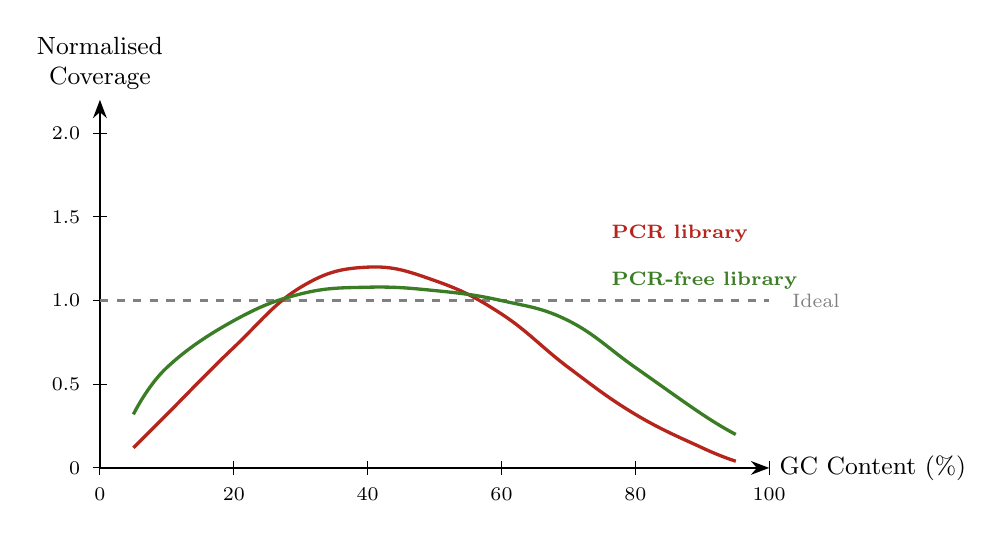
\begin{tikzpicture}[scale=0.85]
  % Axes
  \draw[thick, -{Stealth}] (0,0) -- (10,0) node[right, font=\small] {GC Content (\%)};
  \draw[thick, -{Stealth}] (0,0) -- (0,5.5) node[above, font=\small, align=center] {Normalised\\Coverage};

  % X-axis labels
  \foreach \x/\lab in {0/0, 2/20, 4/40, 6/60, 8/80, 10/100} {
    \draw (\x,-0.1) -- (\x,0.1);
    \node[below, font=\scriptsize] at (\x,-0.15) {\lab};
  }

  % Y-axis labels
  \foreach \y/\lab in {0/0, 1.25/0.5, 2.5/1.0, 3.75/1.5, 5/2.0} {
    \draw (-0.1,\y) -- (0.1,\y);
    \node[left, font=\scriptsize] at (-0.15,\y) {\lab};
  }

  % Ideal line
  \draw[dashed, gray, thick] (0,2.5) -- (10,2.5);
  \node[gray, font=\scriptsize, anchor=west] at (10.2,2.5) {Ideal};

  % PCR library curve (bell-shaped, slightly shifted)
  \draw[very thick, BrickRed] plot[smooth, tension=0.7] coordinates {
    (0.5,0.3) (1,0.8) (2,1.8) (3,2.7) (4,3.0) (5,2.8) (6,2.3) (7,1.5) (8,0.8) (9,0.3) (9.5,0.1)
  };
  \node[BrickRed, font=\scriptsize\bfseries, anchor=west] at (7.5,3.5) {PCR library};

  % PCR-free library curve (flatter)
  \draw[very thick, OliveGreen] plot[smooth, tension=0.7] coordinates {
    (0.5,0.8) (1,1.5) (2,2.2) (3,2.6) (4,2.7) (5,2.65) (6,2.5) (7,2.2) (8,1.5) (9,0.8) (9.5,0.5)
  };
  \node[OliveGreen, font=\scriptsize\bfseries, anchor=west] at (7.5,2.8) {PCR-free library};

\end{tikzpicture}
\caption[GC bias in sequencing.]{Schematic illustration of GC bias. The ideal scenario (dashed grey line) shows uniform coverage across all GC content levels. In practice, libraries prepared with PCR (red) show greater deviation from uniformity than PCR-free libraries (green), with under-representation of both AT-rich and GC-rich regions.}
\label{fig:seqprinciples:gc-bias}
\end{figure}

GC bias can be partially corrected computationally during analysis, and PCR-free library preparation significantly reduces (but does not eliminate) the effect (\cref{fig:seqprinciples:gc-bias}).


% ============================================================
\section{Comparison of Major Sequencing Approaches}
\label{sec:seqprinciples:comparison}

\begin{table}[htbp]
\centering
\caption[Comparison of major sequencing platforms.]{Comparison of the major sequencing technology families as of 2025--2026. Values are approximate and vary by instrument model, chemistry version, and library preparation.}
\label{tab:seqprinciples:platform-comparison}
\small
\begin{tabularx}{\textwidth}{>{\bfseries\raggedright}p{2.8cm} X X X}
\toprule
& \textbf{Illumina (SBS)} & \textbf{PacBio (SMRT)} & \textbf{Oxford Nanopore} \\
\midrule
Read length & 50--300\basepair{} & 10--25\kilobase{} (HiFi); $>$100\kilobase{} (CLR) & Routinely 10--100\kilobase{}; $>$4\megabase{} max \\
\addlinespace
Per-base accuracy & $>$99.9\% (Q30+) & $>$99.9\% (HiFi Q30+); $\sim$87\% (CLR raw) & $\sim$92--98\% (raw); $>$99\% (duplex) \\
\addlinespace
Dominant error type & Substitutions & Insertions (CLR); few errors (HiFi) & Indels (especially in homopolymers) \\
\addlinespace
Throughput per run & Up to $\sim$8\,Tb per 25B flow cell; $\sim$16\,Tb dual-flow-cell run & Up to $\sim$120\gigabase{} per Revio SMRT Cell; $\sim$480\gigabase{} for four cells & Up to $\sim$50\gigabase{} per MinION flow cell or $\sim$200\gigabase{} per current PromethION flow cell \\
\addlinespace
Run time & 12--48 hours & 12--30 hours & Minutes to 72 hours (user-defined) \\
\addlinespace
Base modifications & Requires chemical conversion (e.g., bisulfite) & Direct detection (kinetics) & Direct detection (current signal) \\
\addlinespace
Instrument cost & Quote- and configuration-dependent & Quote- and configuration-dependent & Device or access-plan dependent \\
\addlinespace
Key strengths & Throughput, accuracy, cost per base, ecosystem & HiFi accuracy + length, genome assembly, SV detection & Ultra-long reads, portability, real-time, direct RNA, modifications \\
\addlinespace
Key limitations & Short reads limit repeat resolution and SV detection & Higher cost per base than Illumina & Higher error rate, lower throughput than Illumina \\
\bottomrule
\end{tabularx}
\end{table}

\begin{tipbox}[title={Choosing a Platform}]
No single platform is best for all applications. The choice depends on your experimental question:
\begin{itemize}[nosep]
  \item \textbf{High-throughput quantification} (RNA-seq, ChIP-seq, population-scale WGS): Illumina.
  \item \textbf{Genome assembly, SV detection, haplotype phasing}: PacBio HiFi or ONT.
  \item \textbf{Base modification detection}: ONT (direct) or PacBio (kinetic signatures).
  \item \textbf{Field work and rapid diagnostics}: ONT MinION.
  \item \textbf{Comprehensive analysis}: Many projects now use a combination of short-read and long-read technologies.
\end{itemize}
\end{tipbox}


% ============================================================
\section{The FASTQ File Format}
\label{sec:seqprinciples:fastq}

The primary output of most sequencing instruments (after base calling) is a set of \acrshort{FASTQ} files. Each read in a FASTQ file is represented by four lines:

\begin{lstlisting}[language={},caption={Anatomy of a FASTQ record.},label={lst:seqprinciples:fastq}]
@SEQ_ID read_name and optional description
GATTTGGGGTTCAAAGCAGTATCGATCAAATAGTAAATCCATTTGTTCAACTCACAGTTT
+
!''*((((***+))%%%++)(%%%%).1***-+*''))**55CCF>>>>>>CCCCCCC65
\end{lstlisting}

\begin{enumerate}[itemsep=2pt]
  \item \textbf{Line 1 (Header):} Begins with \texttt{@} followed by a sequence identifier and optional description. Contains information such as instrument name, run ID, flow cell ID, tile number, and cluster coordinates.
  \item \textbf{Line 2 (Sequence):} The raw nucleotide sequence (A, T, G, C, or N for ambiguous bases).
  \item \textbf{Line 3 (Separator):} A \texttt{+} sign (sometimes followed by the same identifier as line 1, but usually just \texttt{+}).
  \item \textbf{Line 4 (Quality):} ASCII-encoded Phred quality scores, one character per base, corresponding to the bases in line 2.
\end{enumerate}

For paired-end sequencing, two FASTQ files are produced: one for ``read 1'' (R1) and one for ``read 2'' (R2). The files are ordered so that the $n$th record in R1 and the $n$th record in R2 correspond to the two ends of the same fragment.


% ============================================================
\section{Summary}
\label{sec:seqprinciples:summary}

This chapter has covered the core principles that underpin all modern sequencing technologies:

\begin{itemize}[itemsep=2pt]
  \item \textbf{All sequencing technologies share} a common logic: fragment, attach adapters, and read bases in a massively parallel fashion.
  \item \textbf{Sequencing by synthesis (SBS)}, used by Illumina, reads bases cycle-by-cycle using fluorescently labelled reversible terminators, producing short, highly accurate reads.
  \item \textbf{Sequencing by ligation} (SOLiD) used fluorescent oligonucleotide probes and a ligase; it is now largely of historical interest.
  \item \textbf{Nanopore sequencing} (Oxford Nanopore) reads DNA or RNA directly by threading single molecules through a protein pore and measuring ionic current disruptions, producing ultra-long reads with direct modification detection.
  \item \textbf{SMRT sequencing} (PacBio) watches a single polymerase in a zero-mode waveguide, producing long HiFi reads with high consensus accuracy.
  \item \textbf{Key metrics} for evaluating sequencing include read length, throughput, accuracy, and error profiles, which differ substantially across platforms.
  \item \textbf{Paired-end} sequencing provides two reads from each fragment, improving alignment, assembly, and variant detection.
  \item \textbf{Coverage} (the average number of times each base is read) is a critical parameter for experimental design, calculated as $N \times L / G$.
  \item \textbf{Multiplexing} uses DNA barcodes (indexes) to combine multiple samples on a single sequencing run, reducing costs.
  \item \textbf{Phred quality scores} quantify the confidence of each base call; Q30 (99.9\% accuracy) is the standard benchmark.
  \item A \textbf{sequencing library} is the collection of adapter-ligated fragments; its complexity determines the amount of unique information available.
  \item \textbf{PCR duplicates} and \textbf{amplification bias} are artefacts of library amplification that can be mitigated by PCR-free protocols and UMIs.
  \item \textbf{GC bias} causes uneven coverage as a function of GC content and is particularly pronounced in PCR-amplified libraries.
\end{itemize}

With these principles established, the following chapters will dive deeper into specific sequencing platforms (Chapters~4--5), library preparation methods (Chapter~6), and the diverse applications of sequencing across genomics, transcriptomics, and epigenomics.


% Part II: Platforms and Technologies
\part{Sequencing Platforms and Technologies}
\chapter{Short-Read Sequencing Platforms}
\label{ch:shortread}

\begin{sourcebox}
Illumina chemistry is anchored by the original whole-genome reversible-terminator demonstration \cite{bentley2008}. Current instrument capacities, prices, and quality guarantees must be tied to a named flow cell, read configuration, document revision, and access date.
\end{sourcebox}

Short-read sequencing---the generation of millions to billions of relatively short DNA sequence reads, typically 50--600 bases in length---remains a workhorse of modern genomics. Since the commercialisation of the first massively parallel sequencing instruments in the mid-2000s, short-read platforms have sharply reduced sequencing reagent cost. A quoted consumables cost, however, is not the total cost of a genome: library preparation, quality control, instrument access, labour, compute, storage, re-runs, interpretation, and required coverage all matter. This chapter surveys the principal platform families without treating vendor list prices or marketing targets as stable scientific facts.

\section{Illumina: The Dominant Platform}
\label{sec:illumina}

\subsection{Historical Context and Market Position}

Illumina Inc.\ (San Diego, California) has dominated the short-read sequencing market since approximately 2010, when its HiSeq~2000 platform became the instrument of choice for large genome centres worldwide. The company's origins trace back to the work of Shankar Balasubramanian and David Klenerman at the University of Cambridge, who developed the sequencing-by-synthesis (SBS) chemistry that underpins all Illumina instruments. Their company, Solexa, was founded in 1998 and acquired by Illumina in 2007 for \$600~million.

By the mid-2010s, Illumina controlled an estimated 80--90\% of the global sequencing market by revenue. Although new competitors have emerged, Illumina remains the reference standard against which all other short-read platforms are measured.

\begin{keyconcept}[title={Illumina's Core Innovation}]
Illumina's key innovation is the combination of \textbf{bridge amplification} on a solid surface (creating clonal clusters of identical DNA molecules) with \textbf{reversible-terminator sequencing by synthesis} (incorporating one fluorescently labelled nucleotide per cycle and imaging the entire flow cell). This massively parallel approach enables billions of DNA fragments to be sequenced simultaneously.
\end{keyconcept}

\subsection{Chemistry: Bridge Amplification and Cluster Generation}

The Illumina sequencing workflow begins with a prepared DNA library---fragments of double-stranded DNA flanked by platform-specific adapter sequences. The critical steps that occur on the flow cell are:

\begin{enumerate}[label=\textbf{Step \arabic*:}, leftmargin=2.5cm]
  \item \textbf{Library denaturation and loading.} The double-stranded library is denatured into single strands and loaded onto the flow cell at a carefully controlled concentration. Too much library leads to overlapping clusters (overclustering); too little wastes capacity.

  \item \textbf{Hybridisation to lawn oligos.} The flow cell surface is coated with a dense lawn of two types of oligonucleotides (P5 and P7) that are complementary to the adapter sequences on the library fragments. Single-stranded library molecules hybridise to these oligos.

  \item \textbf{Extension and bridge formation.} A polymerase extends from the surface-bound oligo, creating a double-stranded bridge. The original template is washed away after denaturation, leaving the covalently attached copy.

  \item \textbf{Bridge amplification.} The newly synthesised strand bends over and hybridises to an adjacent surface oligo of the complementary type, forming a bridge. Polymerase extension creates a double-stranded bridge, which is denatured to yield two surface-bound single strands. This process repeats through approximately 35 cycles of isothermal amplification.

  \item \textbf{Cluster formation.} Each original library molecule generates a clonal cluster of roughly 1{,}000 identical copies, tightly localised on the flow cell surface. These clusters are the unit of signal detection during sequencing.

  \item \textbf{Linearisation.} One strand orientation is selectively cleaved, leaving a lawn of single-stranded molecules all oriented in the same direction, ready for the sequencing primer to hybridise.
\end{enumerate}

\begin{figure}[htbp]
\centering
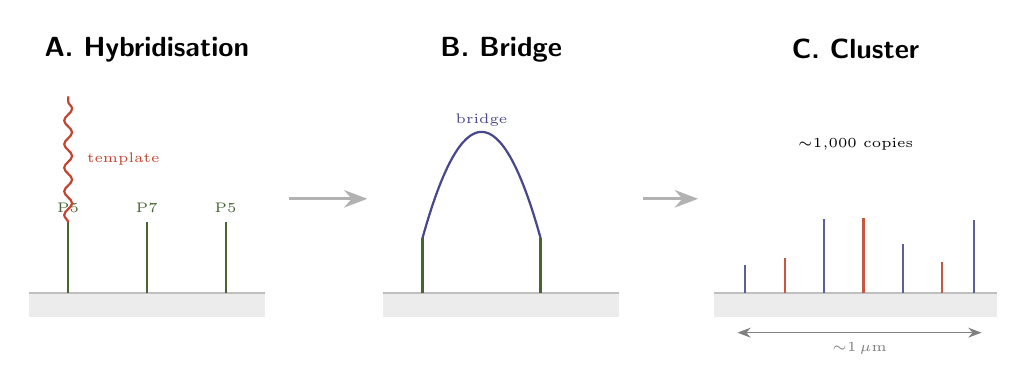
\begin{tikzpicture}[
  >=Stealth,
  oligo/.style={thick, draw=OliveGreen!70!black},
  template/.style={thick, draw=BrickRed!80},
  newstrand/.style={thick, draw=MidnightBlue!80},
  surface/.style={fill=gray!15, draw=gray!40, minimum height=0.4cm},
  label/.style={font=\small\sffamily},
]

% --- Panel A: Hybridisation ---
\node[label, font=\bfseries\sffamily] at (0, 3.4) {A. Hybridisation};
\fill[gray!15] (-1.5, 0) rectangle (1.5, 0.3);
\draw[gray!50, thick] (-1.5, 0.3) -- (1.5, 0.3);
% Surface oligos
\draw[oligo] (-1.0, 0.3) -- (-1.0, 1.2) node[above, font=\tiny, OliveGreen!70!black] {P5};
\draw[oligo] (0, 0.3) -- (0, 1.2) node[above, font=\tiny, OliveGreen!70!black] {P7};
\draw[oligo] (1.0, 0.3) -- (1.0, 1.2) node[above, font=\tiny, OliveGreen!70!black] {P5};
% Template hybridising
\draw[template, decorate, decoration={snake, amplitude=0.5mm, segment length=3mm}]
  (-1.0, 1.2) -- (-1.0, 2.8);
\node[label, BrickRed!80, font=\tiny] at (-0.3, 2.0) {template};

% --- Panel B: Bridge Formation ---
\begin{scope}[xshift=4.5cm]
\node[label, font=\bfseries\sffamily] at (0, 3.4) {B. Bridge};
\fill[gray!15] (-1.5, 0) rectangle (1.5, 0.3);
\draw[gray!50, thick] (-1.5, 0.3) -- (1.5, 0.3);
\draw[oligo] (-1.0, 0.3) -- (-1.0, 1.0);
\draw[oligo] (0.5, 0.3) -- (0.5, 1.0);
% Bridge arc
\draw[newstrand, thick] (-1.0, 1.0) .. controls (-0.5, 2.8) and (0.0, 2.8) .. (0.5, 1.0);
\node[label, MidnightBlue!80, font=\tiny] at (-0.25, 2.5) {bridge};
\end{scope}

% --- Panel C: Denaturation ---
\begin{scope}[xshift=9cm]
\node[label, font=\bfseries\sffamily] at (0, 3.4) {C. Cluster};
\fill[gray!15] (-1.8, 0) rectangle (1.8, 0.3);
\draw[gray!50, thick] (-1.8, 0.3) -- (1.8, 0.3);
% Multiple strands representing a cluster
\foreach \x/\col in {-1.4/MidnightBlue, -0.9/BrickRed, -0.4/MidnightBlue, 0.1/BrickRed, 0.6/MidnightBlue, 1.1/BrickRed, 1.5/MidnightBlue} {
  \draw[\col!70, thick] (\x, 0.3) -- (\x, 1.0+rand*0.4);
}
\node[label, font=\tiny] at (0, 2.2) {${\sim}1{,}000$ copies};
\draw[<->, thin, gray] (-1.5, -0.2) -- (1.6, -0.2) node[midway, below, font=\tiny] {${\sim}1\,\mu$m};
\end{scope}

% Arrows between panels
\draw[->, very thick, gray!60] (1.8, 1.5) -- (2.8, 1.5);
\draw[->, very thick, gray!60] (6.3, 1.5) -- (7.0, 1.5);

\end{tikzpicture}
\caption[Illumina bridge amplification]{Schematic of Illumina bridge amplification. (A)~A single-stranded library molecule hybridises to a surface oligo. (B)~After extension, the strand bends to form a bridge to an adjacent oligo. (C)~Repeated cycles generate a clonal cluster of ${\sim}1{,}000$ identical copies.}
\label{fig:bridge_amp}
\end{figure}

\subsection{Sequencing by Synthesis with Reversible Terminators}

Once clusters have been generated, the actual sequencing proceeds through iterative cycles of nucleotide incorporation and imaging:

\begin{enumerate}[label=\textbf{Cycle step \arabic*:}, leftmargin=3.0cm]
  \item \textbf{Incorporation.} All four nucleotides (A, C, G, T) are flowed across the flow cell simultaneously. Each nucleotide carries (i)~a fluorescent dye and (ii)~a 3\textquotesingle-\textit{O}-azidomethyl blocking group that prevents incorporation of more than one nucleotide per cycle. The polymerase incorporates exactly one complementary nucleotide at each cluster.

  \item \textbf{Wash.} Unincorporated nucleotides are washed away.

  \item \textbf{Imaging.} The flow cell is excited with a laser, and a high-resolution camera captures the fluorescent emission from every cluster. Each cluster emits a colour corresponding to the base just incorporated.

  \item \textbf{Cleavage.} A chemical cleavage step removes both the fluorescent dye and the 3\textquotesingle\ blocking group, regenerating a free 3\textquotesingle-OH ready for the next incorporation.
\end{enumerate}

This cycle repeats for every base of the read. A $2 \times 150$\basepair\ run therefore requires ${\sim}300$ of these cycles (plus additional cycles for index reads).

\begin{figure}[htbp]
\centering
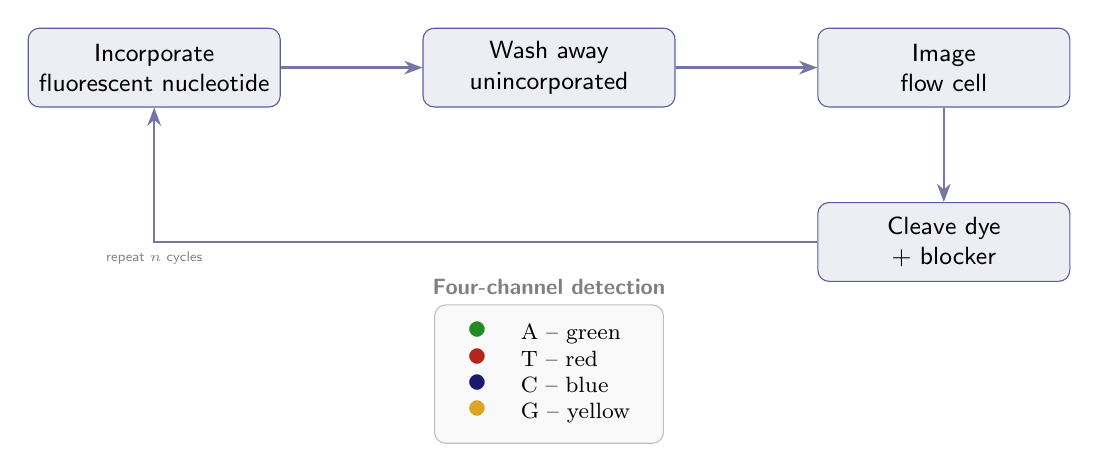
\begin{tikzpicture}[
  >=Stealth,
  node distance=1.8cm,
  boxstep/.style={draw=MidnightBlue!70, fill=MidnightBlue!8, rounded corners=4pt,
    minimum width=3.2cm, minimum height=1.0cm, align=center, font=\small\sffamily},
  arr/.style={->, thick, MidnightBlue!60},
]

\node[boxstep] (inc) {Incorporate\\fluorescent nucleotide};
\node[boxstep, right=of inc] (wash) {Wash away\\unincorporated};
\node[boxstep, right=of wash] (image) {Image\\flow cell};
\node[boxstep, below=1.2cm of image] (cleave) {Cleave dye\\+ blocker};

\draw[arr] (inc) -- (wash);
\draw[arr] (wash) -- (image);
\draw[arr] (image) -- (cleave);
\draw[arr] (cleave) -| (inc) node[midway, below, font=\tiny\sffamily, text=gray] {repeat $n$ cycles};

% Nucleotide detail
\node[below=2.5cm of wash, draw=gray!50, fill=gray!5, rounded corners, inner sep=6pt, font=\footnotesize] (detail) {
  \begin{tabular}{cl}
    \textcolor{ForestGreen}{\Large$\bullet$} & A -- green \\
    \textcolor{BrickRed}{\Large$\bullet$} & T -- red \\
    \textcolor{MidnightBlue}{\Large$\bullet$} & C -- blue \\
    \textcolor{Goldenrod}{\Large$\bullet$} & G -- yellow \\
  \end{tabular}
};
\node[above=0pt of detail, font=\sffamily\footnotesize\bfseries, gray] {Four-channel detection};

\end{tikzpicture}
\caption[Illumina SBS cycle]{The four-step Illumina sequencing-by-synthesis (SBS) cycle. Each cycle adds exactly one base to every cluster, enabling massively parallel read extension.}
\label{fig:sbs_cycle}
\end{figure}

\subsection{Two-Channel vs Four-Channel Chemistry}
\label{sec:twochannel}

Originally, Illumina instruments used \textbf{four-channel chemistry} (4dye/4image), in which each of the four nucleotides carries a spectrally distinct fluorescent dye and each cycle requires four separate images (one per excitation/emission channel). This approach provides unambiguous base identification and is still used on certain instruments such as the NovaSeq~6000 (on some flow cell types) and the older HiSeq series.

To reduce imaging time and cost, Illumina introduced \textbf{two-channel chemistry} (2dye/2image), used on the NextSeq, MiniSeq, and NovaSeq~X series. In this scheme:

\begin{itemize}[nosep]
  \item \textbf{A} is labelled with \textbf{green dye only} (channel~1 positive, channel~2 negative).
  \item \textbf{C} is labelled with \textbf{both green and red dyes} (both channels positive).
  \item \textbf{T} is labelled with \textbf{red dye only} (channel~1 negative, channel~2 positive).
  \item \textbf{G} is \textbf{unlabelled} (both channels negative; identified by absence of signal).
\end{itemize}

\begin{warningbox}[title={G-Base Calling in Two-Channel Chemistry}]
Because G~bases are identified by the \emph{absence} of signal, libraries with very high GC content (or low-diversity libraries such as amplicons) can cause problems on two-channel instruments. If most clusters incorporate G at the same cycle, the software cannot distinguish ``no signal because G'' from ``no signal because the cluster is gone.'' Low-diversity libraries should be spiked with PhiX (a balanced-composition control library) at 20--50\% on two-channel platforms.
\end{warningbox}

\subsection{Patterned vs Non-Patterned Flow Cells}
\label{sec:patterned}

A second major evolution in Illumina hardware was the introduction of \textbf{patterned flow cells}. In traditional non-patterned flow cells (used on MiSeq, HiSeq~2500, and earlier instruments), clusters form at random positions and must be located computationally during the first few cycles. This random seeding limits cluster density because clusters that are too close together merge and become unreadable.

Patterned flow cells, introduced with the HiSeq~3000/4000 and continued in the NovaSeq and NextSeq~1000/2000 series, feature billions of nanowells arranged in a regular grid. Each nanowell captures exactly one library molecule (ideally), producing evenly spaced, uniform clusters. Benefits include:

\begin{itemize}[nosep]
  \item \textbf{Higher cluster density} (and therefore higher output per flow cell).
  \item \textbf{More uniform cluster size}, improving base-calling accuracy.
  \item \textbf{Simplified imaging}, since cluster locations are known \textit{a priori}.
  \item \textbf{Faster run times}, because fewer imaging frames are needed.
\end{itemize}

A disadvantage of patterned flow cells is increased sensitivity to index hopping (discussed in \cref{ch:libprep}), necessitating the use of unique dual indexes (UDIs).


\subsection{Cluster Density Optimisation}
\label{subsec:shortread:cluster-density}

Optimal cluster density is critical for maximising data output while maintaining quality. The relationship between loading concentration, cluster density, and data quality involves a fundamental trade-off:

\begin{itemize}[itemsep=2pt]
  \item \textbf{Under-clustering:} Too few clusters per unit area wastes expensive flow cell real estate. The number of reads is proportional to density, so under-loading linearly reduces output.
  \item \textbf{Over-clustering:} Too many library molecules per nanowell (patterned) or too many overlapping clusters (non-patterned) produce mixed signals that fail quality filtering.
\end{itemize}

For patterned flow cells (NovaSeq, NextSeq 1000/2000), the Poisson statistics of molecular loading govern the fraction of wells with exactly one template. If $\lambda$ is the average number of molecules per well:

\begin{equation}
P(\text{monoclonal well}) = P(k=1) = \lambda e^{-\lambda}
\label{eq:shortread:poisson-loading}
\end{equation}

This is maximised at $\lambda = 1$, where $P(k=1) = e^{-1} \approx 36.8\%$, while $P(k=0) \approx 36.8\%$ (empty wells) and $P(k \geq 2) \approx 26.4\%$ (polyclonal wells). In practice, manufacturers use exclusion amplification (ExAmp) to increase the effective monoclonal fraction by allowing one template to colonise the well before others, achieving effective occupancy rates of 60--80\%.

\begin{keyconcept}[title={Cluster Density and Data Quality}]
Cluster density is specified in units of thousands of clusters per mm$^2$ (K/mm$^2$). Typical target densities are:
\begin{itemize}[nosep]
  \item \textbf{MiSeq (non-patterned):} 800--1,200 K/mm$^2$
  \item \textbf{NovaSeq 6000 S4:} 200--270 K/mm$^2$ (per surface, patterned)
  \item \textbf{NovaSeq X Plus 25B:} $\sim$3,500 K/mm$^2$ (patterned)
\end{itemize}
The percentage of clusters passing filter (\%PF) drops sharply when density exceeds the optimal range and is the primary metric for detecting loading problems.
\end{keyconcept}


\subsection{Phasing and Pre-Phasing Error Models}
\label{subsec:shortread:phasing}

A key source of error in Illumina sequencing is the gradual loss of synchrony among the $\sim$1,000 copies within each cluster. Over successive SBS cycles, two types of desynchronisation occur:

\begin{description}[style=nextline, itemsep=3pt]
  \item[Phasing (lagging)] A fraction $p$ of molecules in a cluster fail to incorporate a nucleotide in a given cycle and ``fall behind'' by one base. These lagging molecules will incorporate one cycle late, contributing a shifted signal.
  \item[Pre-phasing (leading)] A fraction $q$ of molecules incorporate an extra nucleotide (the 3$'$ blocking group fails or is removed prematurely) and ``run ahead'' by one base.
\end{description}

After $n$ cycles, the fraction of molecules still in perfect synchrony with the intended cycle is approximately:

\begin{equation}
f(n) = (1 - p - q)^n
\label{eq:shortread:phasing}
\end{equation}

For typical Illumina phasing ($p \approx 0.1$--$0.25\%$) and pre-phasing ($q \approx 0.05$--$0.15\%$) rates:

\begin{table}[htbp]
\centering
\caption[Signal decay due to phasing.]{Fraction of molecules in synchrony as a function of cycle number, assuming $p = 0.20\%$ and $q = 0.10\%$.}
\label{tab:shortread:phasing}
\small
\begin{tabular}{ccl}
\toprule
\textbf{Cycle $n$} & \textbf{In-phase fraction} & \textbf{Quality impact} \\
\midrule
1 & 99.7\% & Negligible \\
50 & 98.5\% & Minimal \\
100 & 97.0\% & Slight degradation \\
150 & 95.5\% & Noticeable quality drop \\
200 & 94.1\% & Moderate degradation \\
300 & 91.2\% & Significant (R2 of $2 \times 150$) \\
\bottomrule
\end{tabular}
\end{table}

This phasing-induced signal decay is the primary reason why quality scores decline toward the end of Illumina reads, and why Read~2 of a paired-end run typically has slightly lower quality than Read~1 (it is sequenced after additional cycles including the index reads). The basecaller software applies a matrix correction at each cycle to computationally deconvolve the phased signal.


\subsection{Two-Channel Signal Deconvolution}
\label{subsec:shortread:signal-deconvolution}

In two-channel chemistry, each cluster produces a two-dimensional signal vector $(I_{\text{green}}, I_{\text{red}})$ at each cycle. The base call is determined by which of the four quadrants the signal falls into:

\begin{table}[htbp]
\centering
\caption[Two-channel base calling scheme.]{Signal intensity patterns for two-channel base calling.}
\label{tab:shortread:twochannel}
\small
\begin{tabular}{cccl}
\toprule
\textbf{Base} & \textbf{Green ($I_1$)} & \textbf{Red ($I_2$)} & \textbf{Classification} \\
\midrule
A & High & Low & Green-only \\
C & High & High & Both channels \\
G & Low & Low & Neither channel \\
T & Low & High & Red-only \\
\bottomrule
\end{tabular}
\end{table}

The classification boundary between ``high'' and ``low'' is not fixed but is recalibrated at each cycle and each tile using the empirical distribution of intensities. The quality score reflects the distance from the classification boundary: a signal that falls clearly in the A~quadrant receives a high Q~score, while a signal near the boundary between A and G receives a lower Q~score.

Because G~bases produce no signal, the basecaller must distinguish G from cluster loss, low signal due to phasing, or optical noise. This is accomplished by tracking each cluster's signal trajectory across cycles---a cluster that consistently produces signal at most cycles but is dark at the current cycle is called G with high confidence.


\subsection{Index Hopping: Rates and Mitigation}
\label{subsec:shortread:index-hopping}

Index hopping (index switching) occurs when free adapter molecules in the pooled library recombine with other library molecules during the ExAmp on-instrument cluster generation. The rate depends on the platform:

\begin{table}[htbp]
\centering
\caption{Index hopping rates by platform and mitigation strategy.}
\label{tab:shortread:index-hopping}
\small
\begin{tabularx}{\textwidth}{l c X}
\toprule
\textbf{Platform} & \textbf{Typical rate} & \textbf{Mitigation} \\
\midrule
MiSeq (bridge amp) & $<$0.01\% & Not a concern \\
HiSeq 2500 (bridge amp) & $<$0.01\% & Not a concern \\
NovaSeq 6000 (ExAmp) & 0.1--2.0\% & Use UDIs; filter hopped reads \\
NovaSeq X (ExAmp v2) & 0.01--0.1\% & Greatly reduced; UDIs recommended \\
NextSeq 1000/2000 & $<$0.01\% & Bridge amplification; minimal \\
\bottomrule
\end{tabularx}
\end{table}

\textbf{Unique Dual Indexes (UDIs)} solve the index hopping problem by assigning each sample a unique combination of i7 and i5 indexes. With combinatorial dual indexing (CDI), where i7 and i5 indexes are reused across samples in different combinations, a hopped read may be misassigned to the wrong sample. With UDIs, a hopped read will carry an i7 from one sample and an i5 from another---a combination not present in any legitimate sample---and can be computationally discarded.

\begin{warningbox}
For any experiment on a patterned flow cell where sample cross-contamination is unacceptable (e.g., clinical diagnostics, rare variant detection, single-cell experiments), always use UDIs. Combinatorial indexing is only acceptable on platforms that use bridge amplification (MiSeq, NextSeq 1000/2000).
\end{warningbox}


\subsection{Platform Hierarchy}
\label{sec:illumina_platforms}

Illumina offers a portfolio of instruments spanning a wide range of throughput and cost. The major current-generation platforms (as of early 2026) are:

\subsubsection{MiSeq and MiSeq\texorpdfstring{\texttrademark}{(TM)} Dx}

The MiSeq is Illumina's smallest benchtop sequencer, designed for targeted and small-scale experiments. It uses non-patterned flow cells and four-channel chemistry.

\begin{itemize}[nosep]
  \item \textbf{Read lengths:} up to $2 \times 300$\basepair\ (the longest paired-end reads in the Illumina ecosystem).
  \item \textbf{Output:} 0.3--15 Gb per run (depending on the kit version: Nano, Micro, v2, v3).
  \item \textbf{Reads per run:} 1--25 million clusters (single-read equivalents).
  \item \textbf{Run time:} 5--55 hours.
  \item \textbf{Error rate:} $<0.1$\% per base (substitution-dominated).
  \item \textbf{Typical applications:} 16S/ITS amplicon sequencing, small targeted panels, microbial genomes, validation studies, HLA typing.
\end{itemize}

The MiSeq~Dx is the FDA-cleared clinical version, used in regulated diagnostic laboratories.

\subsubsection{NextSeq 1000 and NextSeq 2000}

The NextSeq~1000/2000 are mid-throughput benchtop instruments using patterned flow cells and two-channel chemistry. They replaced the NextSeq~500/550 series.

\begin{itemize}[nosep]
  \item \textbf{Read lengths:} up to $2 \times 150$\basepair\ (NextSeq~2000 supports $2 \times 300$\basepair\ with the P1 300-cycle kit).
  \item \textbf{Output:} 30--360 Gb per flow cell (P1, P2, P3 cartridges of increasing capacity).
  \item \textbf{Reads per run:} 100~million to 1.2~billion clusters.
  \item \textbf{Run time:} 11--48 hours.
  \item \textbf{DRAGEN on-instrument:} built-in FPGA-accelerated secondary analysis (alignment, variant calling).
  \item \textbf{Typical applications:} gene panels, exomes, small genomes, single-cell gene expression (10x Genomics), \gls{RNA-seq}, \gls{ATAC-seq}, low-pass \gls{WGS}.
\end{itemize}

\subsubsection{NovaSeq X and NovaSeq X Plus}

The NovaSeq~X series, launched in 2023 as successors to the NovaSeq~6000, are Illumina's highest-throughput instruments, designed for production-scale sequencing.

\begin{itemize}[nosep]
  \item \textbf{Read lengths:} up to $2 \times 150$\basepair.
  \item \textbf{Output:} for 2$\times$150\basepair{} sequencing, approximately 3--4~Tb per 10B flow cell and 8--10.5~Tb per 25B flow cell; a NovaSeq~X~Plus dual-25B run is specified at approximately 16~Tb in specification sheet M-US-00197 v9.0. The higher end of vendor ranges is not guaranteed.
  \item \textbf{Reads per run:} up to 25~billion clusters per flow cell (25B).
  \item \textbf{Run time:} approximately 13 hours (10B) to 48 hours (25B $2 \times 150$\basepair).
  \item \textbf{Cost:} depends on contract, utilization, region, flow cell, library preparation, and whether the estimate includes only reagents or the full service. Convert a current local quote to cost per usable base rather than relying on a universal number.
  \item \textbf{Flow cell types:} 1.5B, 10B, and 25B (referring to billions of nanowells).
  \item \textbf{DRAGEN on-instrument:} full secondary analysis pipeline.
  \item \textbf{Typical applications:} large-scale population \gls{WGS}, clinical whole-genome/exome sequencing, large \gls{RNA-seq} projects, single-cell atlases, \gls{WGBS}.
\end{itemize}

\begin{tipbox}[title={Choosing an Illumina Flow Cell}]
The 25B flow cell is only cost-effective when you have enough libraries to fill it. Running a single \gls{WGS} sample on a 25B flow cell wastes capacity. Many facilities use the 10B flow cell for routine work and the 25B for large population-scale projects or when many samples are multiplexed together.
\end{tipbox}

\subsection{Illumina Error Profile}

Illumina platforms produce predominantly \textbf{substitution errors}, with a raw per-base error rate of approximately 0.1--0.5\%. The most common systematic errors include:

\begin{itemize}[nosep]
  \item \textbf{GGC motif errors:} elevated substitution rates in GGC trinucleotide contexts.
  \item \textbf{Quality score drop at read ends:} accumulation of incomplete cleavage (phasing) and leading/lagging strand effects.
  \item \textbf{Index hopping:} on patterned flow cells with exclusion amplification (ExAmp), free adapters can re-hybridise to the wrong nanowell during cluster generation, causing barcode misassignment.
\end{itemize}

Insertions and deletions (indels) are rare on Illumina, making the platform well-suited for \gls{SNV} detection but potentially less reliable for homopolymer-length estimation compared to long-read technologies.


\section{MGI / BGI DNBSEQ}
\label{sec:mgi}

MGI Tech (a subsidiary of the BGI Group, Shenzhen, China) has developed a distinct sequencing chemistry and is Illumina's most significant competitor by installed base, particularly in China and parts of Asia and Europe.

\subsection{DNA Nanoball (DNB) Technology}

Rather than bridge amplification, MGI uses \textbf{rolling circle amplification (RCA)} to generate signal:

\begin{enumerate}[nosep]
  \item Library molecules are circularised by ligation of a splint oligonucleotide.
  \item A polymerase with strand-displacement activity performs rolling circle amplification, producing a long concatemer of 200--400 copies of the original molecule, which collapses into a compact \textbf{DNA nanoball} (DNB) roughly 200~nm in diameter.
  \item DNBs are loaded onto a patterned silicon chip with billions of positively charged spots arranged in a regular grid. Each spot captures a single DNB by electrostatic attraction.
\end{enumerate}

\begin{keyconcept}[title={DNA Nanoballs vs Clusters}]
Unlike Illumina clusters, which are formed \emph{on} the flow cell, DNBs are formed \emph{before} loading. This means DNB formation and chip loading are decoupled, offering independent quality-control checkpoints. DNBs are also inherently clonal (derived from a single circular template), virtually eliminating index hopping.
\end{keyconcept}

\subsection{Combinatorial Probe-Anchor Synthesis (cPAS)}

MGI's sequencing chemistry, called \textbf{cPAS} (Combinatorial Probe-Anchor Synthesis), differs from Illumina's \gls{SBS}:

\begin{enumerate}[nosep]
  \item An anchor probe hybridises to a known adapter sequence adjacent to the DNA to be sequenced.
  \item A pool of fluorescently labelled sequencing probes (each representing a specific base) competes for hybridisation to the target position.
  \item After imaging, the anchor--probe complex is stripped, and a new anchor shifted by one base is applied.
\end{enumerate}

The net result is similar to \gls{SBS}: one base is read per cycle per DNB, and the error profile is dominated by substitutions.

\subsection{DNBSEQ Platforms}

\begin{description}[style=nextline, font=\bfseries]
  \item[DNBSEQ-G400 (MGISEQ-2000)] A mid-throughput benchtop instrument. Up to $2 \times 200$\basepair\ reads; 60--720 Gb per run; two independent flow cell positions. Competes with the Illumina NextSeq.

  \item[DNBSEQ-T7] A high-throughput production sequencer. Up to $2 \times 150$\basepair; up to 6~Tb per run with four flow cells; approximately 24-hour run time. Competes with the NovaSeq~6000/X.

  \item[DNBSEQ-T20$\times$2] The latest ultra-high-throughput platform (launched 2024--2025). Two independent sequencing modules, each running two flow cells. Combined output exceeding 10~Tb per run. Aimed at population-scale whole-genome projects.

  \item[DNBSEQ-G99] A compact, low-throughput benchtop system designed for clinical panels and targeted sequencing. Competes with the MiSeq.
\end{description}

\begin{tipbox}[title={Intellectual Property Considerations}]
MGI and Illumina have been involved in extensive patent litigation. Before purchasing MGI instruments, verify the current intellectual property landscape in your jurisdiction. In some markets, licensing agreements are in place; in others, restrictions may apply.
\end{tipbox}


\section{Element Biosciences AVITI}
\label{sec:element}

Element Biosciences (San Diego, California) entered the market in 2022 with the AVITI system, offering what the company terms \textbf{avidity sequencing}.

\subsection{Avidity Sequencing Chemistry}

The AVITI chemistry is based on the following key principles:

\begin{enumerate}[nosep]
  \item \textbf{Rolling circle amplification on the flow cell.} Like MGI, Element uses rolling circle amplification rather than bridge amplification. Library molecules are circularised and then amplified directly on the flow cell surface, producing compact polony (polymerase colony) structures.

  \item \textbf{Avidity base calling.} Rather than labelling individual nucleotides, Element uses multivalent binding of labelled polymer--nucleotide conjugates. The avidity (multipoint binding) of the polymer to the polony provides high signal-to-noise with natural, unmodified nucleotides used for actual incorporation.

  \item \textbf{Non-destructive chemistry.} The labelling polymer is removed after imaging without altering the DNA, potentially reducing cycle-to-cycle artefacts.
\end{enumerate}

\subsection{AVITI Specifications}

\begin{itemize}[nosep]
  \item \textbf{Read lengths:} $2 \times 75$\basepair\ to $2 \times 300$\basepair.
  \item \textbf{Output:} up to 300~Gb per flow cell; the instrument runs two flow cells independently, yielding up to 600~Gb per run.
  \item \textbf{Reads:} up to 1~billion reads per flow cell.
  \item \textbf{Run time:} 16--48 hours depending on read length.
  \item \textbf{Error rate:} $<0.5$\% raw error; primarily substitutions.
  \item \textbf{Cost:} approximately \$1.50--2.50 per Gb, positioning it competitively with the NextSeq~2000 and lower NovaSeq~X tiers.
  \item \textbf{Key differentiator:} Flexible, independent flow cell operation; low instrument cost (approximately \$289{,}000 list price at launch); open library-prep compatibility.
\end{itemize}

\begin{keyconcept}[title={AVITI's Value Proposition}]
Element positions the AVITI as a ``democratisation'' platform---an instrument with high-end data quality at a lower capital cost than a NovaSeq, with the flexibility to run different experiments on its two independent flow cells simultaneously.
\end{keyconcept}


\section{Ultima Genomics}
\label{sec:ultima}

Ultima Genomics (Newark, California) made headlines in 2022 when it announced a target cost of \$1 per Gb---later refined to approximately \$1 per genome at scale.

\subsection{UG~100 Platform}

The Ultima sequencing approach differs substantially from other short-read platforms:

\begin{itemize}[nosep]
  \item \textbf{Natural nucleotide chemistry.} Instead of reversible terminators, the UG~100 uses \emph{natural} (unmodified) nucleotides. Each sequencing cycle flows a single nucleotide species across the flow cell. The polymerase incorporates as many of that nucleotide as the template requires, and the signal from a reporting chemistry indicates \emph{how many} bases were incorporated.

  \item \textbf{Open, circular flow cell.} The flow cell is a large, spinning silicon wafer. Library amplification is performed off-instrument, and DNA polonies are deposited on the wafer surface.

  \item \textbf{High density, single-colour detection.} The simplified chemistry enables very high feature density and reduced imaging requirements.
\end{itemize}

\subsection{Specifications and Considerations}

\begin{itemize}[nosep]
  \item \textbf{Read length:} approximately 300\basepair\ single-end reads.
  \item \textbf{Output:} up to 20~Tb per run.
  \item \textbf{Error profile:} dominated by \textbf{homopolymer-length errors} (systematic miscounting of consecutive identical bases), unlike the substitution errors of Illumina and MGI. This is a direct consequence of the single-nucleotide flow chemistry.
  \item \textbf{Applications:} the platform is particularly suited for applications that are tolerant of single-end reads and where cost per base is paramount, such as population-scale \gls{WGS} and large association studies.
\end{itemize}

\begin{warningbox}[title={Homopolymer Errors on Ultima}]
Because the UG~100 uses natural nucleotides in a flow-based scheme, errors in homopolymer runs (e.g., AAAA\ldots) are the dominant error mode. Bioinformatics pipelines designed for Illumina substitution errors may need adjustment. Ultima provides custom variant-calling tools to handle this error profile.
\end{warningbox}


\section{Singular Genomics G4}
\label{sec:singular}

Singular Genomics (San Diego, California) developed the G4 platform, a benchtop sequencer designed for mid-throughput applications. The instrument uses four independent flow cells, each of which can be started and stopped independently, providing high flexibility for laboratories running diverse projects.

\subsection{Chemistry and Specifications}

\begin{itemize}[nosep]
  \item \textbf{Chemistry:} sequencing by synthesis with fluorescent reversible terminators (conceptually similar to Illumina's approach).
  \item \textbf{Read lengths:} up to $2 \times 150$\basepair.
  \item \textbf{Output:} up to 120~Gb per flow cell; 480~Gb with four flow cells.
  \item \textbf{Reads:} up to 400~million reads per flow cell.
  \item \textbf{Run time:} approximately 8--22 hours per flow cell.
  \item \textbf{Key differentiator:} four independent flow cells on a single instrument, allowing mixed experiment types and staggered starts.
\end{itemize}

\begin{warningbox}[title={Singular Genomics Status}]
Singular Genomics filed for bankruptcy in late 2023 and ceased operations. The G4 is included here for completeness, as some instruments remain in the field, and the technology illustrates alternative design choices. However, no ongoing support, consumable supply, or development is expected.
\end{warningbox}


\section{Comprehensive Platform Comparison}
\label{sec:shortread_comparison}

\Cref{tab:shortread_comparison} provides a side-by-side comparison of the major short-read sequencing platforms available as of early 2026.

\begin{table}[htbp]
\centering
\caption[Short-read sequencing platform comparison]{Comparison of current short-read sequencing platforms. Values are approximate and may vary with kit versions, software updates, and run configurations.}
\label{tab:shortread_comparison}
\small
\renewcommand{\arraystretch}{1.3}
\begin{tabularx}{\textwidth}{@{}l >{\raggedright}X c c c c@{}}
\toprule
\textbf{Platform} & \textbf{Vendor} & \textbf{Max Read Length} & \textbf{Output/Run} & \textbf{Cost/Gb} & \textbf{Run Time} \\
\midrule
MiSeq v3          & Illumina   & $2\times300$\basepair & 15~Gb   & \$100--200  & 5--55\,h   \\
NextSeq 2000 (P3) & Illumina   & $2\times150$\basepair & 360~Gb  & \$15--30    & 11--48\,h  \\
NovaSeq X (10B)   & Illumina   & $2\times150$\basepair & $\sim$3--4~Tb/flow cell  & Quote-dependent & $\sim$22\,h  \\
NovaSeq X Plus (25B) & Illumina & $2\times150$\basepair & $\sim$16~Tb/dual run  & Quote-dependent & $\sim$38\,h  \\
\addlinespace
DNBSEQ-G99        & MGI/BGI    & $2\times150$\basepair & 15~Gb   & \$60--120   & 12--24\,h  \\
DNBSEQ-G400       & MGI/BGI    & $2\times200$\basepair & 720~Gb  & \$8--15     & 24--48\,h  \\
DNBSEQ-T7         & MGI/BGI    & $2\times150$\basepair & 6~Tb    & \$3--5      & 24\,h      \\
DNBSEQ-T20$\times$2 & MGI/BGI  & $2\times150$\basepair & 10+~Tb  & \$2--3      & 24\,h      \\
\addlinespace
AVITI             & Element Bio & $2\times300$\basepair & 600~Gb  & \$1.50--2.50& 16--48\,h \\
\addlinespace
UG 100            & Ultima      & ${\sim}300$\basepair\ SE & 20~Tb & \$1--2     & 20\,h      \\
\addlinespace
G4\fmark{*}       & Singular    & $2\times150$\basepair & 480~Gb  & \$10--20    & 8--22\,h   \\
\bottomrule
\multicolumn{6}{@{}l}{\footnotesize\fmark{*}Singular Genomics ceased operations in late 2023. Included for reference.} \\
\end{tabularx}
\end{table}


\section{How to Choose a Short-Read Platform}
\label{sec:choosing}

Selecting the right short-read platform involves balancing multiple factors. The following decision framework can guide your choice:

\subsection{Throughput Requirements}

\begin{itemize}[nosep]
  \item \textbf{Low throughput} ($<20$~Gb): MiSeq, DNBSEQ-G99. Ideal for amplicons, small panels, microbial genomes.
  \item \textbf{Mid throughput} (20--600~Gb): NextSeq~2000, DNBSEQ-G400, AVITI. Ideal for exomes, targeted panels, \gls{RNA-seq}, single-cell.
  \item \textbf{High throughput} ($>600$~Gb): NovaSeq~X, DNBSEQ-T7/T20, Ultima UG~100. Ideal for \gls{WGS}, population studies, large cohorts.
\end{itemize}

\subsection{Read Length Requirements}

\begin{itemize}[nosep]
  \item \textbf{Short reads} ($2 \times 50$--$100$\basepair): sufficient for most \gls{RNA-seq}, \gls{ChIP-seq}, \gls{ATAC-seq}.
  \item \textbf{Medium reads} ($2 \times 150$\basepair): the standard for \gls{WGS} and exome sequencing.
  \item \textbf{Long short-reads} ($2 \times 250$--$300$\basepair): essential for amplicon sequencing (16S, ITS) where forward and reverse reads must overlap to form a contiguous amplicon. MiSeq and AVITI offer the longest paired-end reads.
\end{itemize}

\subsection{Budget and Capital Expenditure}

\begin{itemize}[nosep]
  \item \textbf{Instrument cost:} ranges from ${\sim}$\$100K (MiSeq) to ${\sim}$\$1M+ (NovaSeq~X~Plus). The AVITI has a competitive list price of ${\sim}$\$289K.
  \item \textbf{Cost per Gb:} inversely correlated with throughput. High-throughput instruments are cheapest per Gb but require high sample volumes to be cost-effective.
  \item \textbf{Service contracts and consumables:} ongoing costs can equal or exceed the instrument cost over 3--5 years.
\end{itemize}

\subsection{Data Ecosystem and Compatibility}

\begin{itemize}[nosep]
  \item \textbf{Software compatibility:} most bioinformatics tools were developed and validated on Illumina data. Newer platforms may require modified parameters or dedicated tools.
  \item \textbf{Library prep compatibility:} Illumina has the broadest library preparation ecosystem. MGI and Element require platform-specific adapters or adapter conversion steps.
  \item \textbf{Regulatory status:} for clinical applications, consider whether the platform has IVD (in vitro diagnostic) clearance in your jurisdiction.
\end{itemize}

\begin{figure}[htbp]
\centering
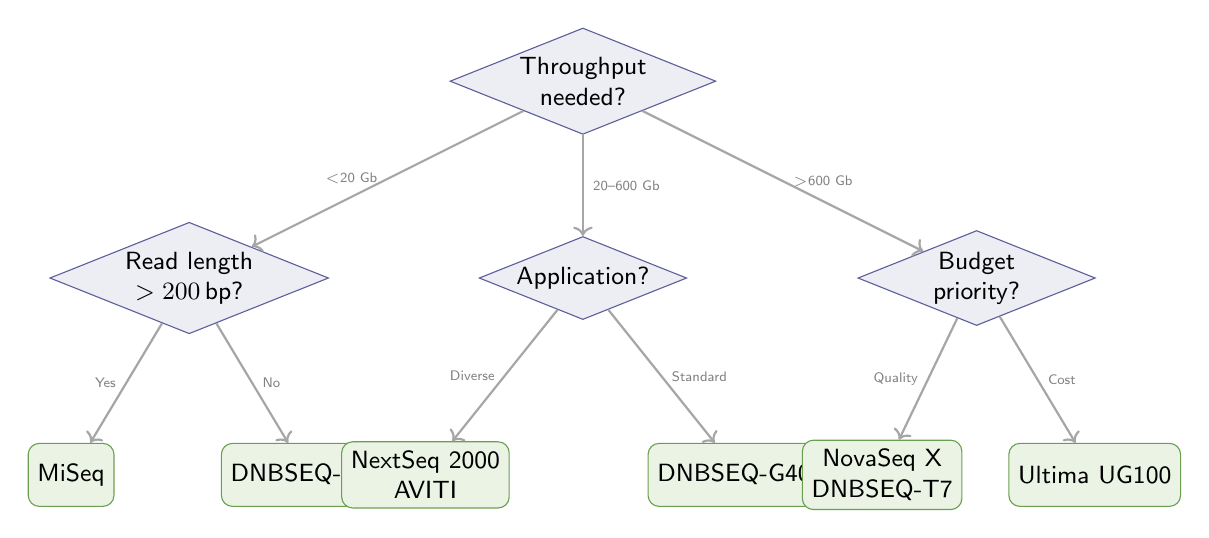
\begin{tikzpicture}[
  decision/.style={diamond, draw=MidnightBlue!70, fill=MidnightBlue!8,
    inner sep=1pt, aspect=2.5, align=center, font=\small\sffamily},
  result/.style={rectangle, draw=OliveGreen!70, fill=OliveGreen!8,
    rounded corners=4pt, minimum height=0.8cm, align=center, font=\small\sffamily},
  arr/.style={->, thick, gray!70},
  lbl/.style={font=\tiny\sffamily, text=gray},
]

\node[decision] (q1) at (0,0) {Throughput\\needed?};
\node[decision] (q2a) at (-5,-2.5) {Read length\\$>200$\basepair?};
\node[decision] (q2b) at (0,-2.5) {Application?};
\node[decision] (q2c) at (5,-2.5) {Budget\\priority?};

\node[result] (r1) at (-6.5,-5) {MiSeq};
\node[result] (r2) at (-3.5,-5) {DNBSEQ-G99};
\node[result] (r3a) at (-2,-5) {NextSeq 2000\\AVITI};
\node[result] (r3b) at (2,-5) {DNBSEQ-G400};
\node[result] (r4) at (3.8,-5) {NovaSeq X\\DNBSEQ-T7};
\node[result] (r5) at (6.5,-5) {Ultima UG100};

\draw[arr] (q1) -- node[lbl, left] {$<$20 Gb} (q2a);
\draw[arr] (q1) -- node[lbl, right] {20--600 Gb} (q2b);
\draw[arr] (q1) -- node[lbl, right] {$>$600 Gb} (q2c);

\draw[arr] (q2a) -- node[lbl, left] {Yes} (r1);
\draw[arr] (q2a) -- node[lbl, right] {No} (r2);
\draw[arr] (q2b) -- node[lbl, left] {Diverse} (r3a);
\draw[arr] (q2b) -- node[lbl, right] {Standard} (r3b);
\draw[arr] (q2c) -- node[lbl, left] {Quality} (r4);
\draw[arr] (q2c) -- node[lbl, right] {Cost} (r5);

\end{tikzpicture}
\caption[Short-read platform decision guide]{Simplified decision flowchart for selecting a short-read sequencing platform. Real decisions involve additional factors including existing infrastructure, bioinformatics support, and vendor relationships.}
\label{fig:shortread_decision}
\end{figure}

\subsection{Practical Considerations}

\begin{protocolbox}[title={Platform Selection Checklist}]
Before committing to a platform, evaluate:
\begin{enumerate}[nosep]
  \item What is my sample throughput per month (number of samples $\times$ required coverage)?
  \item Do I need paired-end reads, and what length?
  \item What is my budget for capital equipment vs.\ consumables?
  \item What bioinformatics tools and pipelines does my team use, and are they validated for this platform's data?
  \item Do I need clinical/regulatory certification?
  \item Is there local service and support from the vendor?
  \item Can I share instrument time with collaborators to improve utilisation?
\end{enumerate}
\end{protocolbox}


\section{Performance Metrics and Quality Considerations}
\label{sec:quality_metrics}

When evaluating short-read platform performance, several key metrics are commonly reported:

\begin{description}[style=nextline, font=\bfseries]
  \item[Q30 (Phred score $\geq$ 30)] The percentage of bases called with at least 99.9\% accuracy. Modern Illumina instruments routinely exceed 85--90\% bases $\geq$~Q30 for $2 \times 150$\basepair\ reads.

  \item[Cluster passing filter (\%PF)] The fraction of clusters that pass quality filters during the first 25 cycles. Values below 70--80\% indicate library or loading problems.

  \item[Error rate by cycle] A cycle-by-cycle plot of mismatch rate against a known reference (often PhiX). Useful for diagnosing phasing problems or chemistry issues.

  \item[Duplication rate] The fraction of reads that are PCR or optical duplicates. High duplication reduces the effective unique coverage and is influenced by library complexity and loading concentration.

  \item[Insert size distribution] For paired-end libraries, the distribution of distances between the two reads of a pair. A tight, symmetric distribution centred on the expected fragment size indicates good library quality.
\end{description}

\begin{tipbox}[title={PhiX Spike-In}]
Always include a small fraction (1--5\%) of PhiX control library in your sequencing run. PhiX provides a balanced-composition, known-sequence control that enables:
\begin{itemize}[nosep]
  \item Calibration of colour balance and focus.
  \item An independent estimate of the per-base error rate.
  \item Diversity boosting for low-complexity libraries (increase to 20--50\% for amplicons on two-channel systems).
\end{itemize}
\end{tipbox}


\section{The Future of Short-Read Sequencing}
\label{sec:shortread_future}

Several trends are shaping the near-term future of short-read sequencing:

\begin{itemize}
  \item \textbf{Continued cost reduction.} The \$100 genome is now achievable in research settings, and further cost decreases will enable routine clinical \gls{WGS} at population scale.

  \item \textbf{Integration of on-instrument analysis.} Illumina's DRAGEN technology and equivalents from other vendors are moving secondary analysis (alignment, variant calling) directly onto the instrument, reducing turnaround time and bioinformatics infrastructure requirements.

  \item \textbf{Increased competition.} The entry of Element, Ultima, and strengthening of MGI provides laboratories with genuine alternatives, driving innovation and price competition.

  \item \textbf{Longer short reads.} Platforms are pushing toward longer reads ($2 \times 300$\basepair\ and beyond) to improve \textit{de novo} assembly and amplicon analysis while retaining the high accuracy of short-read chemistry.

  \item \textbf{Clinical adoption.} Regulatory clearance for sequencing platforms and companion diagnostic assays will continue to expand, making short-read sequencing increasingly mainstream in clinical care.
\end{itemize}

\section{Summary}

Short-read sequencing platforms provide the throughput, accuracy, and cost-effectiveness needed for the vast majority of genomics applications. Illumina remains the dominant player, but MGI, Element Biosciences, and Ultima Genomics offer compelling alternatives with distinct technical approaches. When selecting a platform, consider your throughput needs, read length requirements, budget, and bioinformatics compatibility. The field continues to evolve rapidly, with competition driving costs down and capabilities up.

\chapter{Long-Read Sequencing Platforms}
\label{ch:longread}

\begin{sourcebox}
The technology discussion is anchored by the original SMRT report and an ultra-long nanopore human-genome demonstration \cite{eid2009,jain2018}. PacBio and ONT model, chemistry, yield, and accuracy figures are checked separately against current official specifications.
\end{sourcebox}

While short-read sequencing excels at generating massive volumes of highly accurate data, it has an inherent limitation: individual reads of 100--300 bases cannot span many of the repetitive elements, structural variants, and complex genomic regions that are biologically and clinically important. Long-read sequencing technologies---generating reads from thousands to millions of bases---address these limitations and have opened entirely new areas of genomics research. This chapter provides a comprehensive survey of long-read sequencing platforms, focusing on the two dominant technologies: Pacific Biosciences (PacBio) Single Molecule, Real-Time (SMRT) sequencing and Oxford Nanopore Technologies (ONT) nanopore sequencing.

\section{Why Long Reads Matter}
\label{sec:why_long_reads}

Before diving into platform specifics, it is worth understanding the biological questions that fundamentally require long reads.

\begin{keyconcept}[title={The Long-Read Advantage}]
Long reads provide three capabilities that short reads cannot:
\begin{enumerate}[nosep]
  \item \textbf{Spanning repetitive regions.} Roughly 50\% of the human genome consists of repetitive elements. Short reads cannot be unambiguously placed within repeats longer than the read length. Long reads that span entire repeats resolve their location.
  \item \textbf{Detecting structural variants.} Insertions, deletions, inversions, and translocations larger than a few hundred bases are poorly detected by short reads. Long reads capture both breakpoints of a structural variant in a single read.
  \item \textbf{Phasing haplotypes.} Long reads can link distant variants on the same chromosome, enabling haplotype-resolved (phased) assembly without the need for family data.
\end{enumerate}
\end{keyconcept}

Specific application areas where long reads are essential or strongly preferred include:

\begin{itemize}
  \item \textbf{De novo genome assembly.} Long reads produce contiguous assemblies (high N50 values) that can span centromeres, telomeres, and segmental duplications. The Telomere-to-Telomere (T2T) Consortium used long reads to complete the first truly gapless human reference genome.

  \item \textbf{Structural variant detection.} Clinical and population genetics increasingly recognise that \glspl{SV} (variants $>50$\basepair) account for more variable bases per genome than \glspl{SNV}. Long reads detect SVs with far greater sensitivity and precision.

  \item \textbf{Full-length transcript isoform sequencing.} Long reads can capture entire mRNA molecules (including all exons and UTRs) in a single read, eliminating the need for computational transcript assembly from short-read fragments.

  \item \textbf{Direct base modification detection.} Both PacBio and ONT can detect DNA methylation and other base modifications directly from the sequencing signal, without bisulfite conversion or other chemical treatments.

  \item \textbf{Repetitive region characterisation.} Tandem repeats, microsatellites, and mobile element insertions are resolved by reads long enough to span the entire repeat and anchor into flanking unique sequence.

  \item \textbf{Metagenomics.} Long reads can span entire operons or even full microbial chromosomes, improving species-level classification and enabling the assembly of individual genomes from complex communities.
\end{itemize}


\section{Pacific Biosciences (PacBio)}
\label{sec:pacbio}

\subsection{Historical Context}

Pacific Biosciences (Menlo Park, California) commercialised single-molecule real-time (\gls{SMRTseq}) sequencing in 2011 with the RS system. The technology has undergone continuous improvement through the RS~II, Sequel, Sequel~II, Sequel~IIe, Revio, and Vega systems. PacBio acquired Omniome in 2021; Omniome's sequencing-by-binding chemistry subsequently became the basis of PacBio's short-read Onso instrument.

\subsection{SMRT Sequencing Principle}

The fundamental innovation of PacBio is the ability to observe a single DNA polymerase molecule synthesising a complementary strand in \textbf{real time}.

\subsubsection{Zero-Mode Waveguides (ZMWs)}

The heart of the PacBio system is the \textbf{SMRT Cell}, a chip containing millions of tiny cylindrical holes called \textbf{zero-mode waveguides (ZMWs)}. Each ZMW is approximately 70--100~nm in diameter and 100~nm deep, fabricated in a thin aluminium film deposited on a glass substrate.

The ZMW is so small that its diameter is below the wavelength of the excitation light (${\sim}500$--600~nm). This means that while laser light can enter the well, it decays exponentially---only the bottom 20--30~nm of the well is illuminated. A single polymerase molecule is immobilised at the bottom of each ZMW, and only the nucleotide being incorporated at the active site dwells long enough to produce a detectable fluorescent pulse.

\subsubsection{Evanescent Wave Physics}
\label{subsubsec:longread:evanescent}

The operating principle of the ZMW relies on \textbf{evanescent wave} behaviour. When light encounters an aperture smaller than its wavelength, it cannot propagate through as a freely travelling wave. Instead, the electromagnetic field decays exponentially with distance from the entrance:

\begin{equation}
I(z) = I_0 \, e^{-z/d}
\label{eq:longread:evanescent}
\end{equation}

where $I(z)$ is the light intensity at depth $z$ into the waveguide, $I_0$ is the intensity at the entrance, and $d$ is the \textbf{penetration depth}. For a ZMW of diameter $a$ illuminated at wavelength $\lambda$:

\begin{equation}
d \approx \frac{a}{2} \cdot \frac{1}{\sqrt{(2.405 \cdot \lambda / (\pi a))^2 - 1}}
\label{eq:longread:penetration}
\end{equation}

For typical ZMW dimensions ($a \approx 70$--$100$~nm, $\lambda \approx 532$~nm), the penetration depth $d \approx 20$--$30$~nm. This creates an observation volume of approximately $10^{-21}$ litres (one zeptolitre)---six orders of magnitude smaller than the diffraction limit of conventional optics.

\begin{keyconcept}[title={Why the ZMW Works}]
At micromolar concentrations of fluorescently labelled nucleotides (necessary for polymerase activity), a confocal microscope would observe hundreds of molecules simultaneously, creating overwhelming background fluorescence. The ZMW's zeptolitre observation volume reduces this to an average of $\sim$0.01 freely diffusing molecules in the illuminated zone. Only the nucleotide being incorporated by the polymerase dwells long enough ($\sim$10--100~ms) to produce a detectable pulse above the shot noise of rapidly transiting molecules ($\sim$10~$\mu$s dwell time).
\end{keyconcept}

\begin{figure}[htbp]
\centering
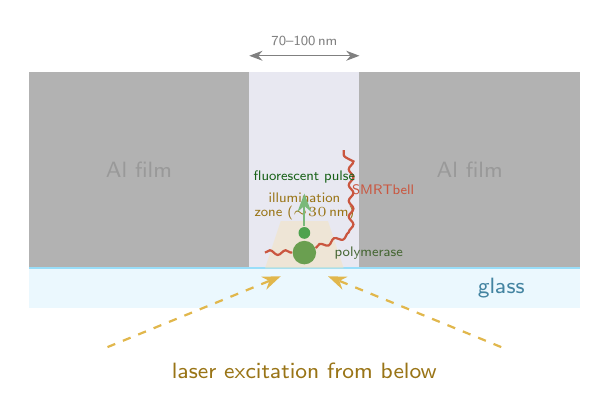
\begin{tikzpicture}[
  >=Stealth,
  scale=1.0,
]

% --- Aluminium layer ---
\fill[gray!60] (-3.5, 0) rectangle (-0.7, 2.5);
\fill[gray!60] (0.7, 0) rectangle (3.5, 2.5);

% --- ZMW well ---
\fill[MidnightBlue!10] (-0.7, 0) rectangle (0.7, 2.5);

% --- Glass substrate ---
\fill[cyan!8] (-3.5, -0.5) rectangle (3.5, 0);
\draw[thick, cyan!40] (-3.5, 0) -- (3.5, 0);

% --- Labels ---
\node[font=\sffamily\footnotesize, gray!80] at (-2.1, 1.25) {Al film};
\node[font=\sffamily\footnotesize, gray!80] at (2.1, 1.25) {Al film};
\node[font=\sffamily\footnotesize, cyan!60!black] at (2.5, -0.25) {glass};

% --- Illumination zone ---
\fill[Goldenrod!30, opacity=0.5] (-0.5, 0) -- (0.5, 0) -- (0.3, 0.6) -- (-0.3, 0.6) -- cycle;
\node[font=\sffamily\tiny, Goldenrod!70!black] at (0, 0.9) {illumination};
\node[font=\sffamily\tiny, Goldenrod!70!black] at (0, 0.7) {zone (${\sim}30$\,nm)};

% --- Polymerase ---
\node[circle, fill=OliveGreen!70, inner sep=3pt] (pol) at (0, 0.2) {};
\node[font=\sffamily\tiny, OliveGreen!70!black, right=3pt of pol] {polymerase};

% --- Template DNA ---
\draw[thick, BrickRed!70, decorate, decoration={snake, amplitude=0.3mm, segment length=2mm}]
  (-0.5, 0.2) -- (pol);
\draw[thick, BrickRed!70, decorate, decoration={snake, amplitude=0.3mm, segment length=2mm}]
  (pol) -- (0.5, 0.4) -- (0.5, 1.5);
\node[font=\sffamily\tiny, BrickRed!70] at (1.0, 1.0) {SMRTbell};

% --- Fluorescent nucleotide ---
\node[circle, fill=ForestGreen!80, inner sep=1.5pt] (nuc) at (0, 0.45) {};
\draw[->, ForestGreen!60, thick] (nuc) -- ++(0, 0.5) node[above, font=\sffamily\tiny, ForestGreen!70!black] {fluorescent pulse};

% --- Laser arrows ---
\draw[->, Goldenrod!80, thick, dashed] (-2.5, -1.0) -- (-0.3, -0.1);
\draw[->, Goldenrod!80, thick, dashed] (2.5, -1.0) -- (0.3, -0.1);
\node[font=\sffamily\footnotesize, Goldenrod!70!black] at (0, -1.3) {laser excitation from below};

% --- Dimensions ---
\draw[<->, thin, gray] (-0.7, 2.7) -- (0.7, 2.7) node[midway, above, font=\tiny\sffamily] {70--100\,nm};

\end{tikzpicture}
\caption[Zero-mode waveguide (ZMW) principle]{Cross-section of a PacBio zero-mode waveguide (ZMW). A single polymerase molecule is immobilised at the bottom of a nanophotonic well. Laser light illuminates only the bottom ${\sim}30$\,nm, so only the nucleotide being incorporated produces a detectable fluorescent signal.}
\label{fig:zmw}
\end{figure}

\subsubsection{The SMRTbell Template}

PacBio library molecules are prepared as \textbf{SMRTbell} constructs: a double-stranded DNA insert flanked by hairpin adapters on both ends, creating a topologically circular (dumbbell-shaped) molecule. The polymerase initiates synthesis at a sequencing primer annealed in the adapter and proceeds around the circular template continuously.

\subsection{Continuous Long Reads (CLR) vs HiFi Reads (CCS)}

PacBio generates two fundamentally different read types from the same instrument:

\subsubsection{Continuous Long Reads (CLR)}

In CLR mode, the polymerase reads around the SMRTbell template as many times as it can before it dissociates or the movie time expires. If the insert is long (e.g., 15--20\kilobase\ or more), the polymerase may traverse the insert only once or a few times, yielding a single long but relatively error-prone read. CLR reads can exceed 100\kilobase, with some reaching beyond 300\kilobase.

\begin{itemize}[nosep]
  \item \textbf{Accuracy:} approximately 85--90\% per-pass (Q10--Q13).
  \item \textbf{Error type:} predominantly insertions and deletions (indels), particularly in homopolymer contexts. Substitution errors are comparatively rare.
  \item \textbf{Strengths:} maximum read length; essential for spanning very large repeats and producing the most contiguous genome assemblies.
\end{itemize}

\subsubsection{HiFi Reads (Circular Consensus Sequencing, CCS)}

If the insert is shorter (typically 10--25\kilobase), the polymerase traverses the circular template multiple times, generating multiple passes (subreads) of the same molecule. These subreads are computationally aligned and a \textbf{consensus} sequence is generated, dramatically reducing the error rate.

\begin{itemize}[nosep]
  \item \textbf{Passes required:} typically 3--10+ passes for high-quality consensus.
  \item \textbf{Accuracy:} $>$Q30 (99.9\%) median per-read accuracy; the best reads exceed Q40.
  \item \textbf{Read length:} typically 10--25\kilobase\ (limited by the requirement for multiple passes within the movie time).
  \item \textbf{Error profile:} residual errors are approximately evenly distributed among substitutions, insertions, and deletions, with no strong systematic biases.
\end{itemize}

\begin{keyconcept}[title={HiFi: The Best of Both Worlds}]
PacBio HiFi reads combine the advantages of long reads (10--25\kilobase) with accuracy rivalling or exceeding that of short reads ($>$Q30). This combination has made HiFi the method of choice for reference-quality genome assembly, clinical structural variant detection, and haplotype-resolved (phased) analysis.
\end{keyconcept}


\subsubsection{CCS Accuracy Model}
\label{subsubsec:longread:ccs-model}

The accuracy improvement from circular consensus sequencing can be modelled quantitatively. If the per-pass (single-subread) error rate is $\varepsilon$ and a position is covered by $N$ independent passes, the consensus error rate $\varepsilon_{\text{CCS}}$ at that position follows a binomial model. For a simple majority-vote consensus, an error occurs only when more than half of the passes contain the same error. The probability of the consensus being wrong is approximately:

\begin{equation}
\varepsilon_{\text{CCS}} \approx \sum_{k=\lceil N/2 \rceil}^{N} \binom{N}{k} \varepsilon^k (1-\varepsilon)^{N-k}
\label{eq:longread:ccs-accuracy}
\end{equation}

For small $\varepsilon$ and moderate $N$, this simplifies to:

\begin{equation}
\varepsilon_{\text{CCS}} \approx \binom{N}{\lceil N/2 \rceil} \varepsilon^{\lceil N/2 \rceil}
\label{eq:longread:ccs-approx}
\end{equation}

In practice, PacBio's \software{ccs} tool uses a more sophisticated approach: it builds a partial-order alignment of all subreads and calls the consensus using a pair-HMM, which accounts for the indel-dominated error profile. The resulting accuracy is:

\begin{table}[htbp]
\centering
\caption[CCS accuracy vs.\ number of passes.]{Expected CCS consensus quality as a function of the number of full passes, assuming $\sim$90\% single-pass accuracy.}
\label{tab:longread:ccs-passes}
\small
\begin{tabular}{ccl}
\toprule
\textbf{Full passes} & \textbf{Consensus quality} & \textbf{Phred equivalent} \\
\midrule
1 & $\sim$90\% & Q10 \\
3 & $\sim$99\% & Q20 \\
5 & $\sim$99.8\% & Q27 \\
7 & $\sim$99.95\% & Q33 \\
10 & $>$99.99\% & $>$Q40 \\
\bottomrule
\end{tabular}
\end{table}


\subsection{PacBio Platforms}

\subsubsection{Revio System}

The Revio, launched in late 2022 and widely deployed from 2023 onward, is PacBio's current flagship production instrument.

\begin{itemize}[nosep]
  \item \textbf{SMRT Cells:} each cell contains approximately 25~million ZMWs.
  \item \textbf{Throughput:} with the SPRQ-Nx specification accessed 1 September 2026, up to approximately 120~Gb of HiFi reads per SMRT Cell and 480~Gb when four cells are run together. Yield depends on insert length and library quality; the maximum is not guaranteed for every library.
  \item \textbf{Movie time:} 24 hours per SMRT Cell (standard).
  \item \textbf{Cost:} contract-, chemistry-, utilization-, and region-dependent; use a current local quote and state whether library preparation and analysis are included.
  \item \textbf{On-instrument analysis:} HiFi read generation (CCS calling) occurs on-instrument in real time using GPUs.
  \item \textbf{Key improvement over Sequel~IIe:} approximately 8-fold increase in throughput per instrument per day, primarily through the 25M ZMW SMRT Cell (vs.\ 8M on Sequel~IIe) and reduced run turnaround.
\end{itemize}

\subsubsection{Vega System}

The Vega, announced in 2024 and commercialised as a benchtop HiFi system, complements rather than replaces the production-scale Revio.

\begin{itemize}[nosep]
  \item \textbf{Positioning:} designed for laboratories seeking HiFi data at lower capital cost and smaller scale.
  \item \textbf{Throughput:} up to approximately 90~Gb per SMRT Cell with the SPRQ-Nx specification accessed 1 September 2026; output depends on library type and run configuration.
  \item \textbf{SMRT Cell format:} uses a new, smaller SMRT Cell format optimised for lower-throughput applications.
  \item \textbf{Workflow simplification:} streamlined library preparation and reduced hands-on time.
\end{itemize}

\subsubsection{Onso (Short-Read Platform)}

PacBio also offers the Onso, a short-read sequencer based on \textbf{Sequencing by Binding (SBB)} chemistry (acquired from Omniome). In SBB, the identity of the next nucleotide is determined by a binding event (without incorporation), followed by separate incorporation of a natural nucleotide. This decoupling of recognition from extension is claimed to reduce context-dependent errors. The Onso competes with Illumina's mid-throughput platforms but is not a long-read instrument and is mentioned here only for completeness.

\subsection{Kinetic Information and Base Modification Detection}

A unique advantage of PacBio SMRT sequencing is that the polymerase's kinetics---specifically, the \textbf{inter-pulse duration} (IPD, the time between fluorescent pulses) and the \textbf{pulse width}---are sensitive to chemical modifications on the template DNA. Modified bases (such as 5-methylcytosine, N6-methyladenine, and others) alter the polymerase's behaviour as it traverses them, producing characteristic kinetic signatures.

\begin{itemize}[nosep]
  \item \textbf{5mC detection:} PacBio HiFi reads can detect 5-methylcytosine (5mC) at CpG sites with high accuracy, using machine learning models trained on kinetic features. This enables simultaneous genome sequencing and methylation profiling without bisulfite conversion.
  \item \textbf{m6A detection:} N6-methyladenine produces a strong kinetic signature and is readily detected even from single-pass CLR data.
  \item \textbf{Other modifications:} various other modifications, including damaged bases, can be detected from kinetic signatures.
\end{itemize}

\begin{tipbox}[title={PacBio Kinetics for Epigenomics}]
If you need both genome sequence and CpG methylation calls from the same experiment, PacBio HiFi is an excellent choice. A single 30$\times$ HiFi whole-genome dataset can provide variant calls, structural variant calls, phased haplotypes, and genome-wide CpG methylation---all without any additional library preparation or chemical treatment.
\end{tipbox}


\section{Oxford Nanopore Technologies (ONT)}
\label{sec:ont}

\subsection{Historical Context}

Oxford Nanopore Technologies (Oxford, United Kingdom) was founded in 2005 as a spin-out from the University of Oxford, based on the pioneering work of Hagan Bayley on protein nanopores. The company's first commercial product, the MinION, was released through an early-access programme (MAP) in 2014. ONT has since expanded its product line to include instruments ranging from the pocket-sized Flongle adapter to the production-scale PromethION, and it remains the only company offering portable, real-time, long-read DNA and RNA sequencing.

\subsection{Nanopore Sequencing Principle}

The fundamental principle of nanopore sequencing is elegantly simple: a single strand of DNA or RNA is driven through a tiny protein pore embedded in an electrically resistant membrane. As each nucleotide passes through the narrowest constriction of the pore, it partially blocks the ionic current flowing through the pore. The pattern of current disruption encodes the sequence.

\begin{figure}[htbp]
\centering
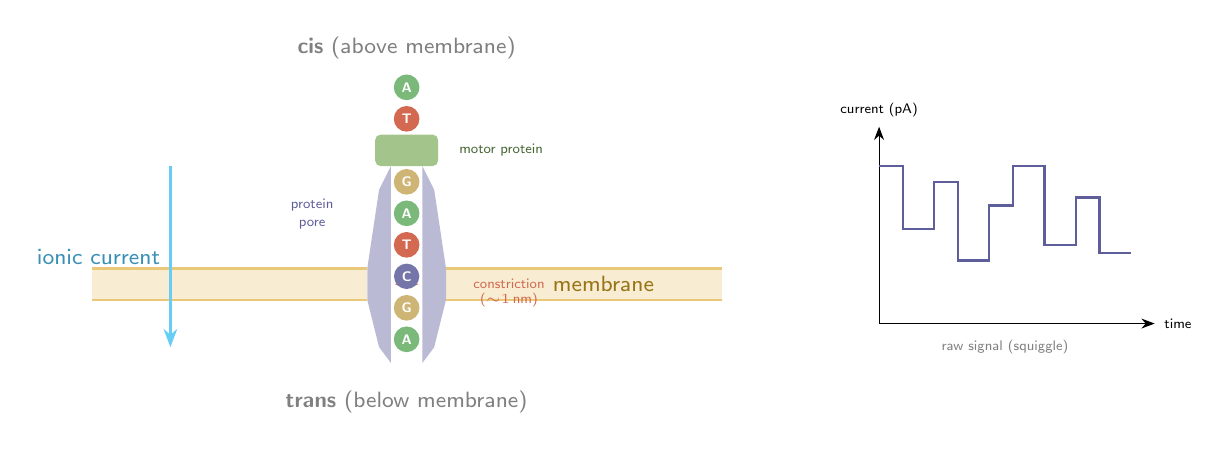
\begin{tikzpicture}[
  >=Stealth,
  scale=1.0,
]

% --- Membrane ---
\fill[Goldenrod!20] (-4, -0.2) rectangle (-0.5, 0.2);
\fill[Goldenrod!20] (0.5, -0.2) rectangle (4, 0.2);
\draw[Goldenrod!60, thick] (-4, 0.2) -- (-0.5, 0.2);
\draw[Goldenrod!60, thick] (0.5, 0.2) -- (4, 0.2);
\draw[Goldenrod!60, thick] (-4, -0.2) -- (-0.5, -0.2);
\draw[Goldenrod!60, thick] (0.5, -0.2) -- (4, -0.2);
\node[font=\sffamily\footnotesize, Goldenrod!70!black] at (2.5, 0) {membrane};

% --- Pore protein ---
\fill[MidnightBlue!30] (-0.5, -0.2) -- (-0.5, 0.2) -- (-0.35, 1.2) -- (-0.2, 1.5)
  -- (-0.2, -1.0) -- (-0.35, -0.8) -- (-0.5, -0.2);
\fill[MidnightBlue!30] (0.5, -0.2) -- (0.5, 0.2) -- (0.35, 1.2) -- (0.2, 1.5)
  -- (0.2, -1.0) -- (0.35, -0.8) -- (0.5, -0.2);

\node[font=\sffamily\tiny, MidnightBlue!70] at (-1.2, 1.0) {protein};
\node[font=\sffamily\tiny, MidnightBlue!70] at (-1.2, 0.75) {pore};

% --- Constriction arrows ---
\draw[<->, thin, BrickRed!60] (-0.15, 0.0) -- (0.15, 0.0);
\node[font=\sffamily\tiny, BrickRed!60] at (1.3, 0.0) {constriction};
\node[font=\sffamily\tiny, BrickRed!60] at (1.3, -0.2) {(${\sim}1$\,nm)};

% --- DNA strand going through ---
\foreach \y/\base/\col in {2.5/A/ForestGreen, 2.1/T/BrickRed, 1.7/C/MidnightBlue, 1.3/G/Goldenrod!80!black, 0.9/A/ForestGreen, 0.5/T/BrickRed, 0.1/C/MidnightBlue, -0.3/G/Goldenrod!80!black, -0.7/A/ForestGreen} {
  \node[circle, fill=\col!60, inner sep=1.5pt, font=\tiny\bfseries\sffamily, text=white] at (0, \y) {\base};
}

% --- Motor protein ---
\fill[OliveGreen!40, rounded corners=2pt] (-0.4, 1.5) rectangle (0.4, 1.9);
\node[font=\sffamily\tiny, OliveGreen!70!black] at (1.2, 1.7) {motor protein};

% --- Current direction ---
\draw[->, thick, cyan!60] (-3.0, 1.5) -- (-3.0, -0.8) node[midway, left, font=\sffamily\footnotesize, cyan!70!black] {ionic current};

% --- Signal trace ---
\begin{scope}[xshift=6cm, yshift=-0.5cm]
\draw[->] (0,0) -- (0, 2.5) node[above, font=\sffamily\tiny] {current (pA)};
\draw[->] (0,0) -- (3.5, 0) node[right, font=\sffamily\tiny] {time};
\draw[thick, MidnightBlue!70]
  (0.0, 2.0) -- (0.3, 2.0) -- (0.3, 1.2) -- (0.7, 1.2) -- (0.7, 1.8)
  -- (1.0, 1.8) -- (1.0, 0.8) -- (1.4, 0.8) -- (1.4, 1.5)
  -- (1.7, 1.5) -- (1.7, 2.0) -- (2.1, 2.0) -- (2.1, 1.0)
  -- (2.5, 1.0) -- (2.5, 1.6) -- (2.8, 1.6) -- (2.8, 0.9) -- (3.2, 0.9);
\node[font=\sffamily\tiny, gray] at (1.6, -0.3) {raw signal (squiggle)};
\end{scope}

% --- Labels ---
\node[font=\sffamily\footnotesize, gray] at (0, 3.0) {\textbf{cis} (above membrane)};
\node[font=\sffamily\footnotesize, gray] at (0, -1.5) {\textbf{trans} (below membrane)};

\end{tikzpicture}
\caption[Nanopore sequencing principle]{The nanopore sequencing principle. A single-stranded DNA molecule is threaded through a protein pore embedded in a lipid membrane. Each nucleotide passing through the constriction produces a characteristic disruption in the ionic current. The resulting ``squiggle'' signal is decoded by neural network basecallers to produce a DNA sequence.}
\label{fig:nanopore}
\end{figure}

\subsubsection{Key Components}

\begin{description}[style=nextline, font=\bfseries]
  \item[Protein pore.] Currently, ONT uses engineered versions of the \textit{CsgG} protein (R10 series pores) embedded in an electrically resistant polymer membrane. The pore contains a dual-constriction region that samples approximately 5--9 nucleotides simultaneously, providing a richer signal than the single-constriction R9.4.1 pore.

  \item[Motor protein.] A helicase enzyme (the ``motor protein'') is attached to the DNA and controls the rate at which the strand passes through the pore---approximately 400--450 bases per second. Without the motor protein, the DNA would translocate too fast for accurate current measurement.

  \item[Adapter and tether.] Library preparation attaches a sequencing adapter (containing the motor protein) to the DNA. A membrane-associated tether helps localise the adapted DNA near the pore.

  \item[ASIC and sensor array.] Each flow cell contains an application-specific integrated circuit (ASIC) with an array of individually addressable electrodes (channels), each capable of hosting one active pore. The ASIC measures the ionic current through each channel at kilohertz sampling rates.
\end{description}


\subsubsection{Nanopore Ion Current Model}
\label{subsubsec:longread:current-model}

The measured ionic current through the nanopore depends on the sequence of nucleotides occupying the constriction region at any given moment. For a pore with a sensing region spanning $k$ nucleotides (a ``$k$-mer context''), each unique $k$-mer produces a characteristic current level. The measured current at time $t$ can be modelled as:

\begin{equation}
I(t) = \mu_{s(t)} + \eta(t)
\label{eq:longread:current-model}
\end{equation}

where $\mu_{s(t)}$ is the expected current level for the $k$-mer $s(t)$ in the constriction at time $t$, and $\eta(t)$ is Gaussian noise. The signal-to-noise ratio (SNR) for distinguishing between two $k$-mers $s_1$ and $s_2$ is:

\begin{equation}
\text{SNR} = \frac{|\mu_{s_1} - \mu_{s_2}|}{\sigma}
\label{eq:longread:snr}
\end{equation}

where $\sigma$ is the standard deviation of the noise. For the R10.4.1 pore with its dual-constriction design, the effective $k$-mer context is approximately $k = 9$ bases, giving $4^9 = 262{,}144$ possible $k$-mers---each with a distinct (though not always easily separable) current level.

\begin{keyconcept}[title={Why Homopolymers Are Hard}]
Homopolymer runs (e.g., AAAAAA) are the dominant error mode in nanopore sequencing because consecutive identical bases produce \textit{the same current level} as they transit the pore. The only information about homopolymer length comes from the \textit{duration} of the signal plateau, which is stochastic: the motor protein does not advance each base at a perfectly constant rate. This duration-to-length mapping is inherently noisier than the current-level-to-identity mapping used for non-homopolymer contexts.
\end{keyconcept}


\subsubsection{Stochastic Models of Homopolymer Errors}
\label{subsubsec:longread:homopolymer}

The time each base spends in the pore constriction (the ``dwell time'') follows a stochastic distribution. For a homopolymer of true length $L$, the total dwell time $T$ is the sum of $L$ independent dwell times:

\begin{equation}
T = \sum_{i=1}^{L} t_i, \quad t_i \sim \text{Gamma}(\alpha, \beta)
\label{eq:longread:dwell-sum}
\end{equation}

The basecaller must infer $L$ from $T$, which is a \textbf{deconvolution problem}. The coefficient of variation of the total dwell time decreases as $1/\sqrt{L}$, but the absolute uncertainty in the estimated length grows. In practice:

\begin{table}[htbp]
\centering
\caption[Homopolymer length accuracy.]{Approximate accuracy of homopolymer length calling for nanopore R10.4.1 + SUP basecalling.}
\label{tab:longread:homopolymer-accuracy}
\small
\begin{tabular}{ccc}
\toprule
\textbf{True length} & \textbf{Accuracy (\% correct)} & \textbf{Common error} \\
\midrule
1--3 & $>$99\% & Rarely miscalled \\
4--5 & 95--99\% & $\pm$1 base \\
6--8 & 85--95\% & $\pm$1 base \\
9--12 & 70--85\% & $\pm$1--2 bases \\
$>$12 & $<$70\% & $\pm$2+ bases \\
\bottomrule
\end{tabular}
\end{table}

\begin{tipbox}
For applications where homopolymer accuracy is critical (e.g., bacterial gene annotation, frameshift detection), consider using PacBio HiFi reads or supplementing nanopore data with short reads for polishing. Duplex nanopore reads (see below) also significantly improve homopolymer accuracy by providing two independent measurements of each base.
\end{tipbox}


\subsection{Library Preparation}

ONT library preparation is notably simpler than that of most other platforms. Two main approaches are offered:

\begin{description}[style=nextline, font=\bfseries]
  \item[Ligation Sequencing Kit (LSK).] The standard high-quality preparation. DNA is end-repaired, A-tailed, and then ligated to ONT sequencing adapters containing the motor protein. This kit preserves the longest fragments and gives the highest throughput. Typical hands-on time: 60--90 minutes.

  \item[Rapid Sequencing Kit (RAD/RBK).] A transposase-based method that fragments the DNA and simultaneously attaches adapters in a single tagmentation step. Library preparation takes approximately 10 minutes, but the transposase cuts the DNA, limiting the maximum read length to the fragment size produced by the enzyme.
\end{description}

\begin{protocolbox}[title={ONT Rapid Library Prep}]
\begin{enumerate}[nosep]
  \item Add transposase to 400~ng of genomic DNA.
  \item Incubate at 30\textdegree C for 1~min, then 80\textdegree C for 1~min.
  \item Add rapid adapter.
  \item Incubate at room temperature for 5~min.
  \item Load onto flow cell.
\end{enumerate}
\textbf{Total time:} $<$15 minutes from extracted DNA to sequencing.
\end{protocolbox}

\subsection{Basecalling: From Signal to Sequence}

Raw nanopore data is not a sequence of bases but a time series of electrical current measurements---the ``squiggle.'' Converting this signal to a DNA sequence is a computationally intensive process called \textbf{basecalling}.

\begin{itemize}
  \item \textbf{Early basecallers} (e.g., Metrichor, Albacore) used hidden Markov models (HMMs) with relatively modest accuracy.

  \item \textbf{Modern basecallers} use deep neural networks. ONT's current production basecaller is \textbf{Dorado}, which succeeded the earlier \textbf{Guppy} and \textbf{Bonito} basecallers. Dorado uses recurrent neural networks (RNNs) and transformer architectures trained on millions of known-sequence reads.

  \item \textbf{Accuracy modes:} Dorado offers multiple models trading speed for accuracy:
    \begin{itemize}[nosep]
      \item \textbf{Fast (SUP-fast):} lowest accuracy, highest speed; suitable for real-time applications.
      \item \textbf{High accuracy (HAC):} good balance of accuracy and speed; the default for most applications.
      \item \textbf{Super accuracy (SUP):} highest accuracy; requires GPU acceleration and is 5--10$\times$ slower than fast mode.
    \end{itemize}

  \item \textbf{Hardware:} production basecalling requires GPU acceleration. A modern NVIDIA GPU (e.g., A100, V100, RTX~4090) can basecall a PromethION flow cell's data in approximately the same time as the run itself.
\end{itemize}

\subsection{Pore Chemistry Evolution: R9 to R10 and Duplex}

\subsubsection{R9.4.1 Pore}

The R9.4.1 pore was ONT's workhorse for many years. It features a single constriction point that reads approximately 5 nucleotides (a 5-mer) simultaneously. This produces a highly compressed signal that made homopolymer detection challenging. Typical simplex (single-strand) accuracy with SUP basecalling was approximately 97--98\% (Q15--Q17).

\subsubsection{R10.4.1 Pore}

The R10.4.1 pore, which has become the standard pore as of 2024--2025, features a \textbf{dual constriction} that reads a longer k-mer context (${\sim}9$ bases). This provides:

\begin{itemize}[nosep]
  \item Significantly improved homopolymer resolution.
  \item Raw simplex accuracy of approximately 99\% (Q20) with SUP basecalling.
  \item Better discrimination of modified bases.
\end{itemize}

\subsubsection{Duplex Reads}

ONT's \textbf{duplex sequencing} exploits the fact that when both strands of a DNA duplex are sequenced in succession through the same pore, the complementary information can be combined to produce a consensus. Duplex reads achieve accuracy exceeding Q30 (99.9\%), approaching PacBio HiFi quality while retaining the potential for very long reads.

\begin{keyconcept}[title={Duplex Reads: ONT's Answer to HiFi}]
Duplex reads are formed when the complement strand immediately follows the template strand through the same nanopore. The two reads of the same molecule provide independent error profiles that, when combined, yield $>$Q30 accuracy. The fraction of reads that are duplex depends on library preparation and loading conditions, typically 30--60\% of reads.
\end{keyconcept}

\subsection{ONT Platform Hierarchy}

Oxford Nanopore offers a range of devices, from portable field instruments to production-scale platforms:

\subsubsection{Flongle}

\begin{itemize}[nosep]
  \item \textbf{Format:} a small, single-use flow cell adapter that plugs into a MinION or GridION.
  \item \textbf{Channels:} 126 (vs.\ 512 on a standard MinION flow cell).
  \item \textbf{Output:} up to 2.8~Gb per flow cell.
  \item \textbf{Cost:} approximately \$90 per flow cell---the lowest entry point for nanopore sequencing.
  \item \textbf{Use cases:} quick experiments, quality checks, small amplicon panels, species identification, teaching.
\end{itemize}

\subsubsection{MinION and MinION Mk1C}

\begin{itemize}[nosep]
  \item \textbf{Format:} the MinION is a USB-powered device roughly the size of a stapler. The Mk1C integrates a touchscreen computer and GPU for on-device basecalling.
  \item \textbf{Channels:} 512.
  \item \textbf{Output:} up to 50~Gb per flow cell (R10.4.1, 72-hour run).
  \item \textbf{Cost:} MinION starter packs begin at approximately \$1{,}000. Flow cells cost approximately \$500--900.
  \item \textbf{Use cases:} field sequencing (pathogen surveillance, biodiversity), small labs, educational settings, rapid diagnostics, proof-of-concept studies.
\end{itemize}

\begin{tipbox}[title={Field Sequencing with MinION}]
The MinION has been used for sequencing in remarkably challenging environments: during the 2014--2016 Ebola outbreak in West Africa, on the International Space Station, in Antarctic field camps, and in tropical forests for real-time biodiversity assessment. Its portability and minimal infrastructure requirements (a laptop and a power source) make it uniquely suited for point-of-need applications.
\end{tipbox}

\subsubsection{GridION}

\begin{itemize}[nosep]
  \item \textbf{Format:} a benchtop device that runs up to 5 MinION-format flow cells simultaneously.
  \item \textbf{Channels:} up to 2{,}560 (5 $\times$ 512).
  \item \textbf{Output:} up to 250~Gb (5 flow cells).
  \item \textbf{Integrated compute:} includes an NVIDIA GPU for real-time basecalling.
  \item \textbf{Use cases:} mid-throughput labs needing flexibility; multiple small projects running in parallel.
\end{itemize}

\subsubsection{PromethION P24 and P48}

\begin{itemize}[nosep]
  \item \textbf{Format:} production-scale instruments running 24 (P24) or 48 (P48) high-capacity flow cells.
  \item \textbf{Channels per flow cell:} approximately 2{,}675 (roughly 5$\times$ a MinION flow cell).
  \item \textbf{Output per flow cell:} current A-Series technical documentation specifies up to 200~Gb per PromethION flow cell. Older promotional material quoted a 290~Gb theoretical maximum, illustrating why an access date and document revision are essential.
  \item \textbf{Total output:} up to approximately 14~Tb (P48, all flow cells).
  \item \textbf{Run time:} typically 72 hours per flow cell.
  \item \textbf{Cost:} access-plan-, contract-, and utilization-dependent; quote the current local total rather than a universal per-flow-cell figure.
  \item \textbf{Use cases:} population-scale \gls{WGS}, large cohort studies, production metagenomics, clinical genome sequencing.
\end{itemize}

\subsection{Ultra-Long Reads}

One of ONT's most remarkable capabilities is the generation of \textbf{ultra-long reads} exceeding 1~Mb (one million bases). Achieving ultra-long reads requires:

\begin{enumerate}[nosep]
  \item \textbf{Ultra-high molecular weight (UHMW) DNA extraction.} Standard extraction methods shear DNA to 20--50\kilobase. For ultra-long reads, specialised gentle lysis protocols (e.g., agarose plug extraction, Circulomics/PacBio Nanobind kits) are used to preserve megabase-length DNA.
  \item \textbf{Careful library preparation.} Wide-bore pipette tips, minimal vortexing, and gravity-driven mixing to avoid shearing.
  \item \textbf{Ligation-based library prep.} Transposase-based (rapid) kits are avoided as they fragment the DNA.
  \item \textbf{Patience.} Ultra-long molecules take hours to translocate through the pore. A 1~Mb read at 400 bases/second takes approximately 42 minutes.
\end{enumerate}

\begin{warningbox}[title={Ultra-Long Read Caveats}]
Ultra-long reads ($>$100\kilobase) are low-throughput by nature: each long molecule occupies a pore for an extended time, reducing the total number of reads. Ultra-long libraries also have lower yields and are technically demanding to prepare. Use ultra-long protocols when the application demands it (e.g., resolving very large repeats or centromeric regions), not as a default.
\end{warningbox}

\subsection{Direct RNA Sequencing}

ONT is currently the only platform capable of sequencing \textbf{native RNA molecules directly}, without reverse transcription to cDNA.

\begin{itemize}
  \item \textbf{Principle.} A poly(A)-tailed RNA molecule is ligated to a sequencing adapter and threaded through the nanopore 3\textquotesingle\ to 5\textquotesingle. The current signal is decoded by RNA-specific basecalling models.

  \item \textbf{Advantages.} Direct RNA sequencing preserves RNA modifications (m6A, pseudouridine, m5C, and others) as detectable signal perturbations. It also eliminates reverse transcription biases and PCR amplification artefacts.

  \item \textbf{Limitations.} Throughput is lower than cDNA-based approaches (the RNA motor protein translocates more slowly). Accuracy is currently lower than DNA basecalling. Input requirements are high (typically 500~ng--1~\textmu g of poly(A)+ RNA).

  \item \textbf{Applications.} Epitranscriptomics research, full-length transcript isoform detection, viral RNA sequencing.
\end{itemize}

\subsection{Adaptive Sampling (Read Until)}

One of ONT's most innovative software features is \textbf{adaptive sampling} (formerly called ``Read Until''). Because nanopore sequencing produces data in real time, the instrument can make decisions about each read while it is being sequenced:

\begin{enumerate}[nosep]
  \item As a DNA molecule begins translocating through the pore, the first few hundred bases are basecalled in real time.
  \item This partial sequence is aligned against a reference or target list.
  \item If the molecule is \textbf{on-target} (matches a region of interest), sequencing continues normally.
  \item If the molecule is \textbf{off-target}, the voltage across that channel is reversed, ejecting the molecule from the pore. The pore is then free to capture a new molecule.
\end{enumerate}

This enables computational enrichment without physical capture or amplification---effectively a ``software pulldown.'' Adaptive sampling can enrich for entire chromosomes, specific genes, or panels of genomic regions, achieving 5--10$\times$ enrichment over random sequencing.

\begin{keyconcept}[title={Adaptive Sampling}]
Adaptive sampling enables selective sequencing of target regions \emph{without any special library preparation}. A whole-genome library is loaded, and the software selectively sequences regions of interest while rejecting off-target molecules in real time. This is unique to nanopore sequencing and has no equivalent on any other platform.
\end{keyconcept}

\subsection{Base Modification Detection}

Like PacBio, ONT can detect base modifications directly from the raw sequencing signal:

\begin{itemize}[nosep]
  \item \textbf{5-methylcytosine (5mC)} at CpG and non-CpG contexts.
  \item \textbf{N6-methyladenine (6mA).}
  \item \textbf{5-hydroxymethylcytosine (5hmC).}
  \item \textbf{RNA modifications} (m6A, pseudouridine) from direct RNA sequencing.
\end{itemize}

Modern ONT basecallers (Dorado) include integrated modification calling models that output modification probabilities alongside the base sequence, producing a ``modBAM'' file containing both sequence and modification information.


\section{PacBio HiFi vs Oxford Nanopore: A Detailed Comparison}
\label{sec:hifi_vs_ont}

\Cref{tab:longread_comparison} provides a comprehensive comparison of the two dominant long-read platforms.

\begin{table}[htbp]
\centering
\caption[PacBio HiFi vs ONT comparison]{Detailed comparison of PacBio HiFi and Oxford Nanopore Technologies for long-read sequencing. Values represent typical performance as of early 2026.}
\label{tab:longread_comparison}
\small
\renewcommand{\arraystretch}{1.3}
\begin{tabularx}{\textwidth}{@{}>{\raggedright\bfseries}p{3.5cm} X X@{}}
\toprule
\textbf{Feature} & \textbf{PacBio HiFi (Revio)} & \textbf{ONT (PromethION, R10.4.1)} \\
\midrule
Read length (typical) & 10--25\kilobase & 10--100\kilobase\ (simplex); ultra-long $>$1\megabase \\
Read length (max) & ${\sim}$25\kilobase\ (HiFi); $>$300\kilobase\ (CLR) & $>$4\megabase\ (record) \\
Per-read accuracy & $>$Q30 (99.9\%) & Q20 simplex (99\%); $>$Q30 duplex \\
Consensus accuracy & $>$Q50 at 30$\times$ & $>$Q50 at 30$\times$ (with R10.4.1) \\
Error type & Balanced (sub, ins, del) & Indels, especially in homopolymers \\
Throughput/cell & Up to ${\sim}$120\gigabase\ HiFi & Up to ${\sim}$200\gigabase\ (current PromethION specification) \\
Throughput/instrument & Up to ${\sim}$480\gigabase\ for four cells & up to 14\,Tb theoretical system output (P48) \\
Run time & 24\,h per cell & 72\,h per flow cell \\
Cost per Gb & Quote-, utilization-, and library-dependent & Access-plan-, utilization-, and library-dependent \\
Cost per 30$\times$ genome & Quote-dependent & Quote-dependent \\
Instrument cost & Quote-dependent & Device and access-plan dependent \\
Portability & Benchtop only & MinION: fully portable \\
Real-time analysis & No (batch processing) & Yes (data streams during run) \\
Adaptive sampling & No & Yes \\
Direct RNA seq & No & Yes \\
Methylation (5mC) & Yes (from kinetics) & Yes (from signal) \\
Library prep time & 4--8 hours & 10 min (rapid) to 90 min (ligation) \\
\bottomrule
\end{tabularx}
\end{table}

\subsection{When to Choose PacBio HiFi}

\begin{itemize}[nosep]
  \item \textbf{Reference-quality genome assembly.} HiFi reads provide the best single-technology assemblies, with per-read accuracy high enough that polishing with short reads is often unnecessary.
  \item \textbf{Clinical structural variant detection.} The high per-read accuracy minimises false positive SV calls.
  \item \textbf{Variant calling in difficult regions.} HiFi accuracy in homopolymers and tandem repeats exceeds ONT simplex.
  \item \textbf{Simultaneous methylation and sequence.} A single HiFi dataset provides sequence, SVs, and CpG methylation.
  \item \textbf{Full-length isoform sequencing (Iso-Seq).} PacBio's Iso-Seq protocol produces full-length transcript sequences with high accuracy.
\end{itemize}

\subsection{When to Choose ONT}

\begin{itemize}[nosep]
  \item \textbf{Ultra-long reads are needed.} Only ONT can routinely produce reads $>$100\kilobase.
  \item \textbf{Field or point-of-care sequencing.} The MinION is the only truly portable sequencer.
  \item \textbf{Real-time results.} Data is available during the run; adaptive sampling enables dynamic targeting.
  \item \textbf{Direct RNA sequencing.} ONT is the only platform that sequences native RNA.
  \item \textbf{Rapid turnaround.} From sample to sequence in under an hour is achievable with rapid library prep.
  \item \textbf{Cost-sensitive large-scale projects.} ONT's cost per Gb can be lower, especially on PromethION.
  \item \textbf{Complex epigenomic profiling.} Detection of diverse modification types (5mC, 5hmC, 6mA) from a single dataset.
\end{itemize}

\begin{tipbox}[title={Complementary Technologies}]
PacBio and ONT are not mutually exclusive. Many cutting-edge genome projects use both: ONT ultra-long reads for scaffolding and spanning the largest repeats, combined with PacBio HiFi for base-level accuracy and variant calling. The T2T human genome used both technologies extensively.
\end{tipbox}


\section{Hybrid Sequencing Approaches}
\label{sec:hybrid}

Combining short and long reads leverages the strengths of both technologies:

\begin{description}[style=nextline, font=\bfseries]
  \item[Short reads for accuracy, long reads for contiguity.] A common assembly strategy uses long reads for the initial contig assembly and short reads for error correction (polishing). With PacBio HiFi achieving $>$Q30 natively, the need for short-read polishing has diminished for PacBio-based assemblies, but it remains valuable for ONT-only assemblies.

  \item[Short reads for coverage, long reads for phasing.] A cost-effective clinical strategy uses deep short-read \gls{WGS} for comprehensive variant calling, supplemented by moderate long-read coverage for SV detection and haplotype phasing.

  \item[Linked reads as a middle ground.] Technologies such as 10x Genomics Chromium (now discontinued but widely used in existing datasets) and Universal Sequencing Technology's TELL-Seq add long-range information to short reads through molecular barcoding. While not true long reads, linked reads provide phase information and improve SV detection.

  \item[Hi-C for scaffolding.] Chromosome conformation capture data (Hi-C, discussed in \cref{ch:libprep} and later chapters) provides chromosome-scale scaffolding information that complements both short and long reads.
\end{description}

\begin{table}[htbp]
\centering
\caption[Hybrid sequencing strategies]{Common hybrid sequencing strategies and their applications.}
\label{tab:hybrid_strategies}
\small
\renewcommand{\arraystretch}{1.3}
\begin{tabularx}{\textwidth}{@{}>{\raggedright}p{3.2cm} >{\raggedright}p{3.2cm} X@{}}
\toprule
\textbf{Strategy} & \textbf{Typical Coverage} & \textbf{Primary Application} \\
\midrule
HiFi only (30$\times$) & 30$\times$ HiFi & Reference-quality assembly, clinical WGS \\
ONT + Illumina & 30$\times$ ONT + 30$\times$ Illumina & Cost-effective assembly with polishing \\
ONT ultra-long + HiFi & 30$\times$ ONT-UL + 30$\times$ HiFi & T2T-grade assembly \\
HiFi + Hi-C & 30$\times$ HiFi + Hi-C & Chromosome-scale phased assembly \\
Illumina + low-pass ONT & 30$\times$ Illumina + 5--10$\times$ ONT & Clinical WGS with SV detection \\
\bottomrule
\end{tabularx}
\end{table}


\section{Emerging Long-Read Developments}
\label{sec:longread_emerging}

The long-read sequencing landscape continues to evolve:

\begin{itemize}
  \item \textbf{PacBio Vega.} The Vega system aims to make HiFi sequencing more accessible to smaller laboratories with lower capital cost and simplified workflows.

  \item \textbf{ONT pore improvements.} ONT continues to develop new pore proteins with improved resolution and accuracy. Future pores may achieve Q30+ simplex accuracy routinely, further closing the gap with HiFi.

  \item \textbf{ONT P2 Solo.} A lower-cost PromethION variant running two flow cells, targeting labs that need PromethION-class data without the full P24/P48 instrument.

  \item \textbf{Direct protein sequencing.} ONT has demonstrated proof-of-concept for reading amino acid sequences through nanopores, potentially extending the platform beyond nucleic acids.

  \item \textbf{Electronic signal improvements.} Both platforms are investing in improved signal processing and AI-based basecalling, with each generation of basecaller software improving accuracy without hardware changes.

  \item \textbf{Multi-modal data.} The ability of both platforms to simultaneously call bases and modifications is evolving toward richer ``multi-omic'' readouts from single molecules.
\end{itemize}


\section{Summary}

Long-read sequencing has matured from an error-prone niche technology to a mainstream tool capable of producing highly accurate, phased genome assemblies and detecting the full spectrum of genetic variation. PacBio HiFi offers the highest per-read accuracy in a long-read format, making it ideal for reference-quality assembly and clinical applications. Oxford Nanopore provides unmatched read length, portability, real-time analysis, and unique capabilities such as direct RNA sequencing and adaptive sampling. The choice between platforms---or the decision to combine them---depends on the specific biological question, required read length and accuracy, budget, and infrastructure constraints. Together, these technologies are completing our picture of genome biology in ways that short reads alone could never achieve.

\chapter{Library Preparation: From Sample to Sequencer}
\label{ch:libprep}

Every sequencing experiment, regardless of platform, begins with the transformation of a biological sample into a \textbf{sequencing library}: a collection of DNA (or cDNA) fragments that carry the platform-specific adapter sequences required for cluster generation (or equivalent amplification), priming, and sequencing. Library preparation is arguably the most critical step in the entire sequencing workflow---poor library quality cannot be rescued by downstream bioinformatics. This chapter covers the complete library preparation process, from nucleic acid extraction through quality control, with detailed discussion of specific protocols, multiplexing strategies, and common failure modes.

\section{What Is a Sequencing Library?}
\label{sec:what_is_library}

\begin{keyconcept}[title={Definition of a Sequencing Library}]
A \textbf{sequencing library} is a collection of DNA fragments of defined size range, each carrying platform-specific adapter sequences at both ends. These adapters serve multiple functions:
\begin{itemize}[nosep]
  \item \textbf{Binding} the fragment to the flow cell surface (or bead, or ZMW).
  \item \textbf{Priming} the sequencing reaction (providing a known sequence for the sequencing primer to hybridise).
  \item \textbf{Indexing/barcoding} the fragment so that multiple samples can be pooled and sequenced together (multiplexing) and then computationally separated after sequencing (demultiplexing).
  \item \textbf{Amplification priming} during optional PCR enrichment of the library.
\end{itemize}
\end{keyconcept}

The general workflow for preparing a sequencing library consists of:

\begin{enumerate}[nosep]
  \item Nucleic acid extraction.
  \item Fragmentation (for DNA libraries; RNA is typically already fragmented or is fragmented during protocol steps).
  \item End repair and A-tailing.
  \item Adapter ligation.
  \item Size selection (optional, depending on protocol).
  \item PCR amplification (optional; PCR-free protocols exist).
  \item Library quantification and quality control.
\end{enumerate}

\begin{figure}[htbp]
\centering
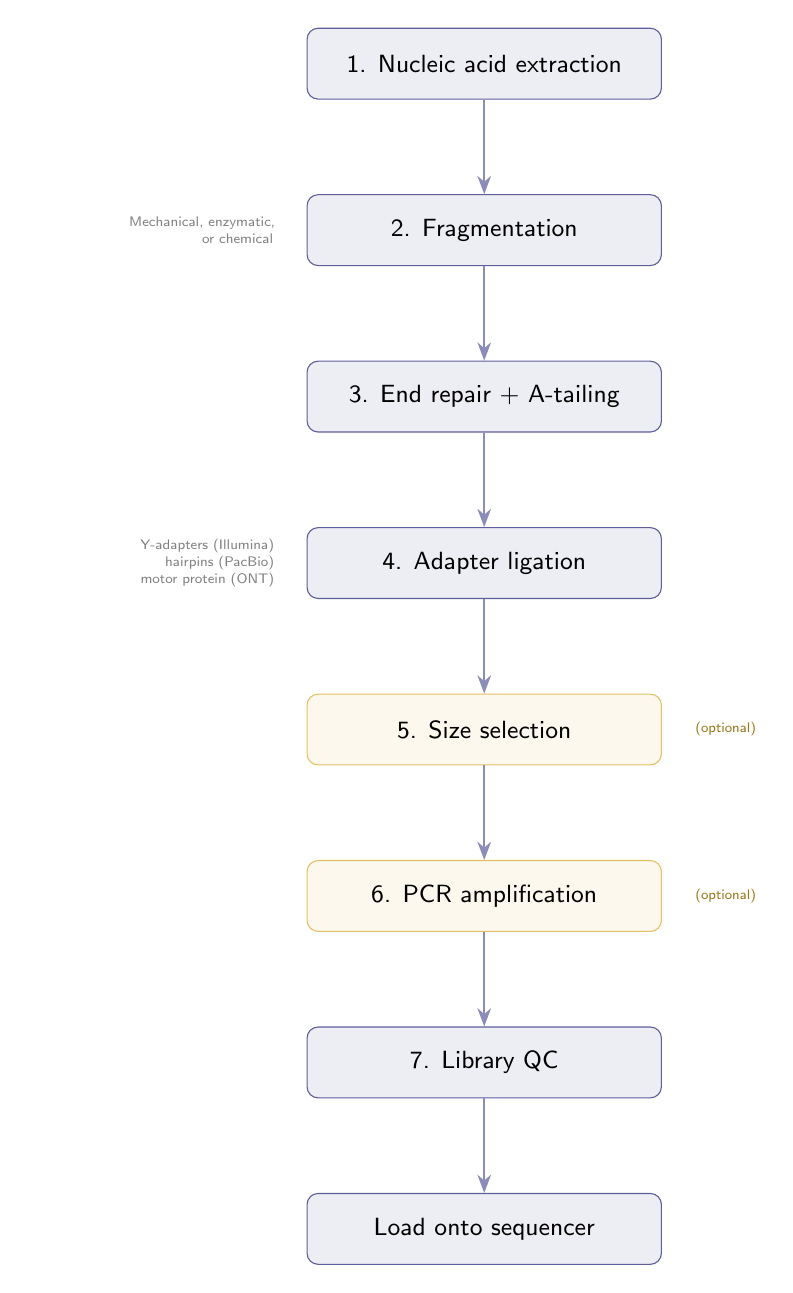
\begin{tikzpicture}[
  >=Stealth,
  node distance=1.2cm,
  wfstep/.style={draw=MidnightBlue!70, fill=MidnightBlue!8, rounded corners=4pt,
    minimum width=4.5cm, minimum height=0.9cm, align=center, font=\small\sffamily},
  optional/.style={draw=Goldenrod!70, fill=Goldenrod!8, rounded corners=4pt,
    minimum width=4.5cm, minimum height=0.9cm, align=center, font=\small\sffamily},
  arr/.style={->, thick, MidnightBlue!50},
]

\node[wfstep] (extract) {1. Nucleic acid extraction};
\node[wfstep, below=of extract] (frag) {2. Fragmentation};
\node[wfstep, below=of frag] (endrepair) {3. End repair + A-tailing};
\node[wfstep, below=of endrepair] (ligate) {4. Adapter ligation};
\node[optional, below=of ligate] (size) {5. Size selection};
\node[optional, below=of size] (pcr) {6. PCR amplification};
\node[wfstep, below=of pcr] (qc) {7. Library QC};
\node[wfstep, below=of qc] (seq) {Load onto sequencer};

\draw[arr] (extract) -- (frag);
\draw[arr] (frag) -- (endrepair);
\draw[arr] (endrepair) -- (ligate);
\draw[arr] (ligate) -- (size);
\draw[arr] (size) -- (pcr);
\draw[arr] (pcr) -- (qc);
\draw[arr] (qc) -- (seq);

% Optional labels
\node[font=\tiny\sffamily, Goldenrod!70!black, right=0.3cm of size] {(optional)};
\node[font=\tiny\sffamily, Goldenrod!70!black, right=0.3cm of pcr] {(optional)};

% Annotations
\node[font=\tiny\sffamily, gray, left=0.3cm of frag, text width=3cm, align=right] {Mechanical, enzymatic,\\or chemical};
\node[font=\tiny\sffamily, gray, left=0.3cm of ligate, text width=3cm, align=right] {Y-adapters (Illumina)\\hairpins (PacBio)\\motor protein (ONT)};

\end{tikzpicture}
\caption[General library preparation workflow]{Overview of the general sequencing library preparation workflow. Gold-coloured steps are optional depending on the specific protocol. The entire process transforms extracted nucleic acids into adapter-ligated fragments ready for sequencing.}
\label{fig:libprep_workflow}
\end{figure}


\section{Nucleic Acid Extraction}
\label{sec:extraction}

The first step is obtaining high-quality nucleic acid from the biological sample. The choice of extraction method depends on the sample type (tissue, blood, cells, FFPE, environmental), the nucleic acid type (DNA vs.\ RNA), and the downstream application (especially the required fragment length for long-read sequencing).

\subsection{DNA Extraction Methods}

\subsubsection{Column-Based Extraction}

Column-based kits (e.g., QIAGEN DNeasy, Zymo Quick-DNA) use silica membranes that selectively bind DNA in the presence of chaotropic salts. The workflow consists of lysis, binding, washing, and elution.

\begin{itemize}[nosep]
  \item \textbf{Advantages:} fast (30--60 minutes), reproducible, minimal hands-on time, good purity (A260/280 $\geq$ 1.8).
  \item \textbf{Disadvantages:} shears DNA to 20--50\kilobase\ (unsuitable for ultra-long read preps). Limited input capacity.
  \item \textbf{Best for:} short-read sequencing, PCR-based applications, standard long-read preps where $>$50\kilobase\ reads are not required.
\end{itemize}

\subsubsection{Bead-Based Extraction}

Magnetic bead kits (e.g., Omega Bio-tek Mag-Bind, Beckman Coulter GenFind, PacBio Nanobind) use paramagnetic beads coated with silica or other DNA-binding matrices.

\begin{itemize}[nosep]
  \item \textbf{Advantages:} automatable (liquid-handling robots), scalable, gentler than columns (can preserve longer fragments with optimised protocols). The PacBio Nanobind (formerly Circulomics) kits use large paramagnetic discs that minimise shearing and can yield DNA $>$100\kilobase.
  \item \textbf{Disadvantages:} requires magnetic rack; some kits have lower yields than columns.
  \item \textbf{Best for:} high-throughput extraction, long-read sequencing, automation.
\end{itemize}

\subsubsection{Phenol-Chloroform Extraction}

The traditional organic extraction method remains the gold standard for yield and purity from difficult samples.

\begin{itemize}[nosep]
  \item \textbf{Procedure:} cell lysis with SDS and proteinase~K, organic extraction with phenol:chloroform:isoamyl alcohol (25:24:1), aqueous phase recovery, ethanol precipitation or SPRI bead cleanup.
  \item \textbf{Advantages:} highest yields, excellent purity, can handle large and difficult samples (e.g., plant tissue, insects).
  \item \textbf{Disadvantages:} uses toxic chemicals (phenol is corrosive and a suspected carcinogen), time-consuming, difficult to automate, requires a fume hood.
  \item \textbf{Best for:} challenging samples, when maximum yield is essential, ultra-high molecular weight DNA for ultra-long nanopore reads.
\end{itemize}

\begin{warningbox}[title={DNA Integrity for Long-Read Sequencing}]
For PacBio HiFi or ONT long-read sequencing, DNA integrity is critical. Degraded or highly sheared DNA will produce short reads regardless of the sequencing platform's capabilities. Always assess DNA integrity using pulsed-field gel electrophoresis (PFGE) or the Agilent Femto Pulse / AATI Fragment Analyzer before committing to a long-read library preparation.
\end{warningbox}

\subsection{RNA Extraction Methods}

RNA is chemically less stable than DNA due to the 2\textquotesingle-OH on the ribose sugar, which makes it susceptible to alkaline hydrolysis. RNA is also readily degraded by ubiquitous RNases. RNA extraction therefore requires strict RNase-free technique.

\subsubsection{TRIzol (Guanidinium Thiocyanate-Phenol-Chloroform)}

\begin{itemize}[nosep]
  \item \textbf{Principle:} guanidinium thiocyanate denatures proteins (including RNases); phenol-chloroform extraction separates RNA into the aqueous phase.
  \item \textbf{Advantages:} high yield, works from diverse tissues, extracts total RNA (including small RNAs).
  \item \textbf{Disadvantages:} organic solvents, time-consuming, potential genomic DNA contamination.
\end{itemize}

\subsubsection{Column-Based RNA Extraction}

Kits such as QIAGEN RNeasy and Zymo Quick-RNA provide silica column purification with optional on-column DNase digestion.

\begin{itemize}[nosep]
  \item \textbf{Advantages:} fast, reproducible, DNase treatment integrated, good for automation.
  \item \textbf{Disadvantages:} lower yield than TRIzol from some tissues; may lose small RNAs unless specifically captured.
\end{itemize}

\subsubsection{mRNA Selection vs rRNA Depletion}

Total RNA is composed of approximately 80--85\% ribosomal RNA (rRNA), which is usually uninformative for gene expression studies. Two strategies address this:

\begin{itemize}
  \item \textbf{Poly(A) selection:} oligo(dT) beads capture polyadenylated mRNA. Effective and widely used, but excludes non-polyadenylated transcripts (many lncRNAs, histone mRNAs, prokaryotic mRNAs).
  \item \textbf{rRNA depletion:} probe-based methods (e.g., Illumina Ribo-Zero, NEB NEBNext rRNA Depletion) hybridise to rRNA and remove it, retaining all other RNA species. Necessary for prokaryotic \gls{RNA-seq}, total RNA studies, and when non-coding RNAs are of interest.
\end{itemize}

\begin{tipbox}[title={Choosing Between Poly(A) Selection and rRNA Depletion}]
\begin{itemize}[nosep]
  \item For standard eukaryotic gene expression profiling, \textbf{poly(A) selection} provides cleaner data with less intronic/intergenic noise.
  \item For degraded samples (e.g., FFPE tissue), use \textbf{rRNA depletion}---degraded RNA loses its poly(A) tails.
  \item For prokaryotic or mixed samples, \textbf{rRNA depletion} is essential (prokaryotic mRNAs lack poly(A) tails).
  \item For non-coding RNA studies, use \textbf{rRNA depletion} to retain all non-ribosomal transcripts.
\end{itemize}
\end{tipbox}


\section{Fragmentation}
\label{sec:fragmentation}

Genomic DNA is far too long (chromosomes are megabases to hundreds of megabases) to be sequenced directly on short-read platforms. Fragmentation reduces the DNA to a defined size range suitable for the sequencing platform and application.

\subsection{Mechanical Fragmentation}

\subsubsection{Sonication (Covaris)}

The most widely used mechanical fragmentation method employs focused acoustic energy (Covaris ultrasonicators). DNA in solution is subjected to high-frequency acoustic waves that create cavitation, shearing the DNA at random positions.

\begin{itemize}[nosep]
  \item \textbf{Fragment size:} tunable from 150\basepair\ to 5\kilobase\ by adjusting power, duty cycle, and time.
  \item \textbf{Advantages:} highly reproducible, produces a tight fragment-size distribution, no sequence bias.
  \item \textbf{Disadvantages:} requires specialised equipment (Covaris instrument), limited throughput (one sample at a time for some models), DNA ends are damaged and require end repair.
\end{itemize}

\subsubsection{Nebulisation and Hydroshear}

Older mechanical methods include nebulisation (forcing DNA through a small orifice under gas pressure) and hydroshearing (forcing DNA through a small tube). These are largely superseded by Covaris but may be encountered in legacy protocols.

\subsection{Enzymatic Fragmentation}

\subsubsection{Tagmentation (Tn5 Transposase)}

Tagmentation uses a hyperactive mutant of the Tn5 transposase loaded with sequencing adapters. The transposase simultaneously fragments the DNA and inserts adapters in a single step (``cut-and-paste'' transposition). This is the basis of the Illumina DNA Prep (formerly Nextera DNA Flex) kit.

\begin{itemize}[nosep]
  \item \textbf{Advantages:} extremely fast (minutes), requires very low input (as little as 1~ng), simultaneously fragments and tags, reducing the number of protocol steps.
  \item \textbf{Disadvantages:} Tn5 has known insertion-site preferences (bias toward open chromatin and certain sequence motifs), which can create non-uniform genome coverage. Fragment size is controlled by the enzyme:DNA ratio and is less precisely tunable than Covaris.
  \item \textbf{Applications:} Illumina DNA Prep, ATAC-seq (where the Tn5 insertion bias is actually the signal of interest), ONT rapid library prep.
\end{itemize}

\paragraph{Quantifying Tn5 Insertion Bias.}
\label{par:libprep:tn5-bias}

The hyperactive Tn5 transposase exhibits a measurable sequence preference at its insertion site. Studies have revealed a consensus insertion motif centred on the 9\basepair{} target site duplication:

\begin{itemize}[itemsep=2pt]
  \item \textbf{Position +1/+9 (flanking the duplication):} strong preference for weak bases (A/T), with $\sim$70\% AT frequency versus the expected 50--60\%.
  \item \textbf{Central positions:} mild preference for alternating purine-pyrimidine patterns.
  \item \textbf{Chromatin context:} in native chromatin (as in ATAC-seq), Tn5 preferentially inserts into nucleosome-free regions. On purified DNA, the bias is purely sequence-dependent.
\end{itemize}

The practical consequence is that tagmentation-based libraries show up to $\pm$20\% deviation from expected coverage at extreme GC compositions compared to $\pm$5--10\% for Covaris-based libraries. This bias is modest for most applications but can be significant for quantitative analyses in GC-extreme organisms (e.g., \species{Plasmodium falciparum} at $\sim$19\% GC or \species{Streptomyces} at $\sim$72\% GC).

\begin{figure}[htbp]
\centering
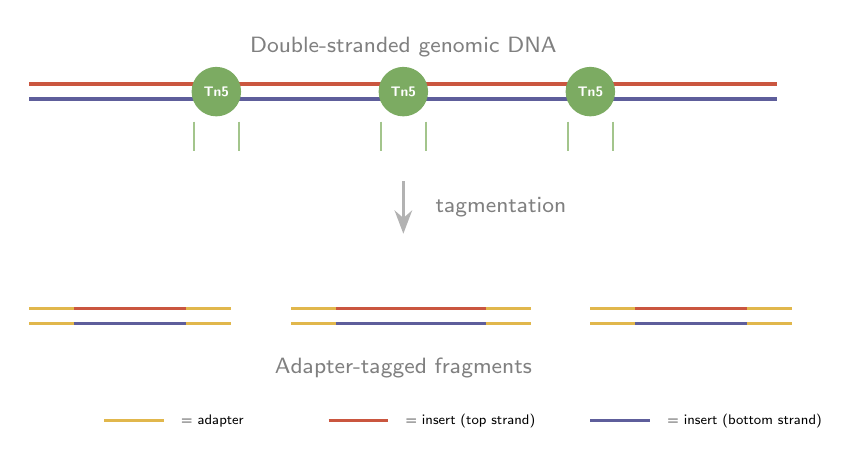
\begin{tikzpicture}[
  >=Stealth,
  scale=0.95,
]

% --- Input DNA ---
\draw[very thick, BrickRed!70] (0, 0) -- (10, 0);
\draw[very thick, MidnightBlue!70] (0, -0.2) -- (10, -0.2);
\node[font=\sffamily\footnotesize, gray] at (5, 0.5) {Double-stranded genomic DNA};

% --- Tn5 enzymes ---
\foreach \x in {2.5, 5.0, 7.5} {
  \node[circle, fill=OliveGreen!60, inner sep=3pt, font=\tiny\bfseries\sffamily, text=white] at (\x, -0.1) {Tn5};
  \draw[OliveGreen!40, thick] (\x-0.3, -0.5) -- (\x-0.3, -0.9);
  \draw[OliveGreen!40, thick] (\x+0.3, -0.5) -- (\x+0.3, -0.9);
}

% Arrow
\draw[->, very thick, gray!60] (5, -1.3) -- (5, -2.0);
\node[font=\sffamily\footnotesize, gray, right] at (5.3, -1.65) {tagmentation};

% --- Fragmented DNA with adapters ---
\begin{scope}[yshift=-3cm]
  % Fragment 1
  \draw[very thick, Goldenrod!80] (0, 0) -- (0.6, 0);
  \draw[very thick, BrickRed!70] (0.6, 0) -- (2.1, 0);
  \draw[very thick, Goldenrod!80] (2.1, 0) -- (2.7, 0);
  \draw[very thick, Goldenrod!80] (0, -0.2) -- (0.6, -0.2);
  \draw[very thick, MidnightBlue!70] (0.6, -0.2) -- (2.1, -0.2);
  \draw[very thick, Goldenrod!80] (2.1, -0.2) -- (2.7, -0.2);

  % Fragment 2
  \draw[very thick, Goldenrod!80] (3.5, 0) -- (4.1, 0);
  \draw[very thick, BrickRed!70] (4.1, 0) -- (6.1, 0);
  \draw[very thick, Goldenrod!80] (6.1, 0) -- (6.7, 0);
  \draw[very thick, Goldenrod!80] (3.5, -0.2) -- (4.1, -0.2);
  \draw[very thick, MidnightBlue!70] (4.1, -0.2) -- (6.1, -0.2);
  \draw[very thick, Goldenrod!80] (6.1, -0.2) -- (6.7, -0.2);

  % Fragment 3
  \draw[very thick, Goldenrod!80] (7.5, 0) -- (8.1, 0);
  \draw[very thick, BrickRed!70] (8.1, 0) -- (9.6, 0);
  \draw[very thick, Goldenrod!80] (9.6, 0) -- (10.2, 0);
  \draw[very thick, Goldenrod!80] (7.5, -0.2) -- (8.1, -0.2);
  \draw[very thick, MidnightBlue!70] (8.1, -0.2) -- (9.6, -0.2);
  \draw[very thick, Goldenrod!80] (9.6, -0.2) -- (10.2, -0.2);

  \node[font=\sffamily\footnotesize, gray] at (5, -0.8) {Adapter-tagged fragments};

  % Legend
  \draw[very thick, Goldenrod!80] (1, -1.5) -- (1.8, -1.5);
  \node[font=\sffamily\tiny, right] at (1.9, -1.5) {= adapter};
  \draw[very thick, BrickRed!70] (4, -1.5) -- (4.8, -1.5);
  \node[font=\sffamily\tiny, right] at (4.9, -1.5) {= insert (top strand)};
  \draw[very thick, MidnightBlue!70] (7.5, -1.5) -- (8.3, -1.5);
  \node[font=\sffamily\tiny, right] at (8.4, -1.5) {= insert (bottom strand)};
\end{scope}

\end{tikzpicture}
\caption[Tagmentation with Tn5 transposase]{Tagmentation: the Tn5 transposase simultaneously fragments double-stranded DNA and inserts sequencing adapters at the cut sites. This combines fragmentation, end repair, and adapter attachment into a single enzymatic step.}
\label{fig:tagmentation}
\end{figure}

\subsubsection{Enzymatic Fragmentation (dsDNA Fragmentase)}

NEB's dsDNA Fragmentase and similar enzyme cocktails use a combination of a nicking enzyme and a recombinase to produce random double-strand breaks. Fragment size is controlled by incubation time and temperature.

\begin{itemize}[nosep]
  \item \textbf{Advantages:} no specialised equipment needed, compatible with standard lab equipment.
  \item \textbf{Disadvantages:} less reproducible than Covaris; time-sensitive (over-digestion is easy).
\end{itemize}

\subsection{Chemical Fragmentation}

RNA fragmentation for \gls{RNA-seq} is typically achieved by incubation in alkaline buffer or divalent cations (Mg$^{2+}$) at elevated temperature (e.g., 94\textdegree C for 1--8 minutes). The fragmentation time controls the resulting size distribution. This is a standard step in most RNA-seq library prep protocols.


\section{End Repair and A-Tailing}
\label{sec:endrepair}

After fragmentation, DNA ends are heterogeneous: they may have overhangs, blunt ends, damaged bases, or 5\textquotesingle-hydroxyl groups. Before adapters can be ligated, the ends must be repaired:

\begin{enumerate}[nosep]
  \item \textbf{End repair:} a combination of T4 DNA polymerase (fills in 5\textquotesingle\ overhangs, removes 3\textquotesingle\ overhangs) and T4 polynucleotide kinase (phosphorylates 5\textquotesingle\ ends) converts all fragments to blunt-ended, 5\textquotesingle-phosphorylated molecules.

  \item \textbf{A-tailing:} Klenow fragment (exo-) adds a single deoxyadenosine (A) overhang to the 3\textquotesingle\ end of each fragment. This A-overhang is complementary to the T-overhang on most Illumina adapters, providing a non-palindromic sticky end that (i)~increases ligation efficiency and (ii)~prevents fragment--fragment concatenation.
\end{enumerate}

Most modern kits combine end repair and A-tailing into a single reaction (e.g., NEB Ultra~II End Prep Enzyme Mix).


\section{Adapter Ligation}
\label{sec:adapters}

Adapters are short, synthetic oligonucleotide constructs that are ligated to the prepared DNA fragments. Their structure varies by platform:

\subsection{Illumina Y-Adapters}

Illumina adapters have a distinctive \textbf{Y-shape} (forked adapter). The double-stranded region ligates to the DNA fragment, while the single-stranded arms carry the P5 and P7 sequences (for flow cell binding) and primer sites for sequencing and index reads.

\begin{figure}[htbp]
\centering
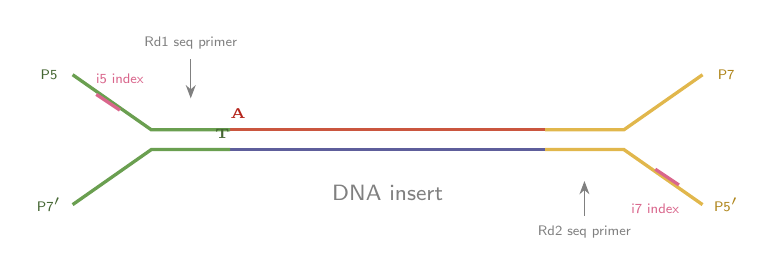
\begin{tikzpicture}[
  >=Stealth,
  scale=1.0,
]

% --- Insert DNA ---
\draw[very thick, BrickRed!70] (-2, 0) -- (2, 0);
\draw[very thick, MidnightBlue!70] (-2, -0.25) -- (2, -0.25);
\node[font=\sffamily\footnotesize, gray] at (0, -0.8) {DNA insert};

% --- Left Y-adapter ---
\draw[very thick, OliveGreen!70] (-2, 0) -- (-3.0, 0) -- (-4.0, 0.7);
\draw[very thick, OliveGreen!70] (-2, -0.25) -- (-3.0, -0.25) -- (-4.0, -0.95);
\node[font=\sffamily\tiny, OliveGreen!70!black] at (-4.3, 0.7) {P5};
\node[font=\sffamily\tiny, OliveGreen!70!black] at (-4.3, -0.95) {P7$'$};

% --- Right Y-adapter ---
\draw[very thick, Goldenrod!80] (2, 0) -- (3.0, 0) -- (4.0, 0.7);
\draw[very thick, Goldenrod!80] (2, -0.25) -- (3.0, -0.25) -- (4.0, -0.95);
\node[font=\sffamily\tiny, Goldenrod!80!black] at (4.3, 0.7) {P7};
\node[font=\sffamily\tiny, Goldenrod!80!black] at (4.3, -0.95) {P5$'$};

% --- Index regions ---
\draw[very thick, purple!60] (-3.4, 0.25) -- (-3.7, 0.45);
\node[font=\sffamily\tiny, purple!60] at (-3.4, 0.65) {i5 index};
\draw[very thick, purple!60] (3.4, -0.5) -- (3.7, -0.7);
\node[font=\sffamily\tiny, purple!60] at (3.4, -1.0) {i7 index};

% --- Sequencing primer sites ---
\draw[<-, thin, gray] (-2.5, 0.4) -- (-2.5, 0.9) node[above, font=\tiny\sffamily, gray] {Rd1 seq primer};
\draw[<-, thin, gray] (2.5, -0.65) -- (2.5, -1.1) node[below, font=\tiny\sffamily, gray] {Rd2 seq primer};

% --- T-overhang ---
\node[font=\tiny\bfseries, BrickRed] at (-1.9, 0.2) {A};
\node[font=\tiny\bfseries, OliveGreen!70!black] at (-2.1, -0.05) {T};

\end{tikzpicture}
\caption[Illumina Y-adapter structure]{Structure of an Illumina Y-adapter (forked adapter) ligated to a DNA insert. The double-stranded stem ligates to the A-tailed fragment via a complementary T-overhang. The single-stranded arms carry the P5 and P7 flow cell binding sequences, index sequences (i5, i7), and sequencing primer annealing sites.}
\label{fig:y_adapter}
\end{figure}

After adapter ligation:
\begin{itemize}[nosep]
  \item \textbf{Read~1} is sequenced from the Read~1 primer site, reading through the insert toward the opposite adapter.
  \item \textbf{Index~1 (i7)} is read after Read~1, identifying the sample.
  \item \textbf{Index~2 (i5)} is read after resynthesis of the complementary strand.
  \item \textbf{Read~2} is sequenced from the Read~2 primer site in the opposite direction.
\end{itemize}

\subsection{PacBio SMRTbell Adapters}

PacBio uses \textbf{hairpin adapters} that are ligated to both ends of the double-stranded insert, creating a topologically circular molecule (the SMRTbell). This circular structure enables the polymerase to read around the molecule multiple times for HiFi consensus generation.

\subsection{ONT Adapters}

ONT adapters contain the \textbf{motor protein} (helicase) pre-loaded onto the adapter. During ligation, the adapter--motor complex is attached to the end of the DNA. When the adapted molecule encounters a nanopore, the motor protein engages and controls the translocation rate.


\section{Size Selection}
\label{sec:size_selection}

After ligation, the library typically contains a range of fragment sizes. Size selection narrows this range to the optimal window for the application and platform.

\subsection{SPRI Bead-Based Size Selection (AMPure XP)}

The most widely used size-selection method employs \textbf{Solid Phase Reversible Immobilisation (SPRI) beads} (Beckman Coulter AMPure XP or equivalent). DNA binds to the carboxyl-coated paramagnetic beads in the presence of polyethylene glycol (PEG) and salt; the size selectivity is controlled by the ratio of beads to sample.

\begin{itemize}[nosep]
  \item \textbf{High bead:sample ratio} (e.g., 1.8$\times$): binds fragments down to ${\sim}$100\basepair.
  \item \textbf{Low bead:sample ratio} (e.g., 0.6$\times$): binds only large fragments ($>$500\basepair), effectively removing small fragments and adapter dimers.
  \item \textbf{Double-sided selection:} a two-step protocol (e.g., 0.55$\times$ followed by 0.8$\times$) removes both large and small fragments, yielding a tight size distribution centred on the desired range.
\end{itemize}

\begin{protocolbox}[title={Double-Sided SPRI Size Selection (Target: 300--500\,bp)}]
\begin{enumerate}[nosep]
  \item Add 0.55$\times$ volume of SPRI beads to the library. Mix and incubate 5~min.
  \item Place on magnet. \textbf{Transfer supernatant} (contains fragments $<$600\basepair) to a new tube. Discard beads (large fragments bound).
  \item Add 0.25$\times$ \emph{additional} beads to the supernatant (total ratio now ${\sim}$0.8$\times$). Mix and incubate 5~min.
  \item Place on magnet. \textbf{Discard supernatant} (contains fragments $<$200\basepair, including adapter dimers).
  \item Wash beads twice with 80\% ethanol.
  \item Elute in 30~\textmu L EB or water. The eluted library is enriched for 300--500\basepair\ fragments.
\end{enumerate}
\end{protocolbox}

\subsection{Gel-Based Size Selection}

\begin{itemize}[nosep]
  \item \textbf{BluePippin / PippinHT (Sage Science):} automated gel electrophoresis with electroelution of size-selected fractions. Highly precise (narrow size distributions), essential for some applications (e.g., PacBio HiFi libraries targeting a specific insert size).
  \item \textbf{Manual gel extraction:} excision of the desired band from an agarose gel followed by gel purification (e.g., QIAGEN QIAquick). Low throughput, risk of UV damage, but still used in some protocols.
\end{itemize}

\begin{warningbox}[title={Adapter Dimers}]
Adapter dimers (two adapters ligated together without an insert) are the most common library preparation artefact. They are preferentially sequenced because they are small and cluster efficiently. Even a small fraction of adapter dimers can consume a large proportion of sequencing reads. Always verify dimer removal by Bioanalyzer/TapeStation before sequencing. If dimers are present, perform an additional SPRI cleanup at 0.8$\times$ ratio.
\end{warningbox}


\subsection{The Physics of SPRI Bead Size Selection}
\label{subsec:libprep:spri-physics}

SPRI (Solid Phase Reversible Immobilisation) bead-based selection exploits the principle that DNA solubility in a PEG/NaCl solution depends on fragment length. The mechanism involves molecular crowding: PEG excludes volume, effectively increasing the local concentration of DNA and salt, forcing DNA out of solution and onto the negatively charged carboxyl bead surface (mediated by divalent cation bridging).

The critical PEG concentration for precipitation of a DNA fragment of length $L$ scales approximately as:

\begin{equation}
[\text{PEG}]_{\text{crit}} \propto L^{-0.5}
\label{eq:libprep:spri-scaling}
\end{equation}

This means that longer fragments precipitate (bind to beads) at lower PEG concentrations than shorter fragments. Since the bead:sample ratio directly controls the effective PEG concentration (the beads are suspended in a PEG/NaCl buffer), the ratio controls the size cutoff:

\begin{table}[htbp]
\centering
\caption[SPRI bead ratio and size cutoff.]{Approximate relationship between AMPure XP bead:sample volume ratio and the minimum fragment size retained.}
\label{tab:libprep:spri-ratios}
\small
\begin{tabular}{cl}
\toprule
\textbf{Bead:sample ratio} & \textbf{Approximate size cutoff} \\
\midrule
2.0$\times$ & $\geq$50\basepair{} (captures nearly everything) \\
1.8$\times$ & $\geq$100\basepair{} (standard cleanup) \\
1.0$\times$ & $\geq$200\basepair{} \\
0.8$\times$ & $\geq$300\basepair{} \\
0.65$\times$ & $\geq$400\basepair{} \\
0.5$\times$ & $\geq$600\basepair{} \\
0.4$\times$ & $\geq$800\basepair{} \\
\bottomrule
\end{tabular}
\end{table}

\begin{tipbox}[title={Optimising SPRI Ratios}]
The exact size cutoff at a given ratio depends on the buffer composition of your sample. Carry-over ethanol, high salt concentrations, or detergents can shift the effective cutoff. When precision matters (e.g., PacBio HiFi library prep), always validate your SPRI ratios empirically using a Bioanalyzer or TapeStation trace before and after selection.
\end{tipbox}


\subsection{Adapter Design: Thermodynamic Considerations}
\label{subsec:libprep:adapter-thermo}

Sequencing adapters are carefully engineered oligonucleotides whose design is constrained by multiple thermodynamic requirements:

\begin{itemize}[itemsep=2pt]
  \item \textbf{Melting temperature ($T_m$) matching:} The double-stranded portion of Y-adapters must have a $T_m$ high enough to remain annealed at the ligation temperature (typically 20$\,^\circ$C) but low enough to denature cleanly during cluster generation (typically 95--98$\,^\circ$C). A $T_m$ of 60--72$\,^\circ$C is typical for Illumina adapters.
  \item \textbf{Minimal secondary structure:} Self-complementary regions must be avoided to prevent adapter hairpins and self-dimers. The free energy of the most stable intramolecular structure should be $\Delta G > -2$ kcal/mol.
  \item \textbf{Balanced GC content:} Adapter sequences are designed with 40--60\% GC content to ensure uniform hybridisation and amplification.
  \item \textbf{Index sequence design:} Barcode sequences must maintain minimum Hamming distance ($d \geq 3$ for single-error correction, $d \geq 5$ for double-error correction) and balanced base composition at each position across the index set. Illumina's IDT for Illumina indexes are designed with $d \geq 4$ and colour balance at every cycle.
\end{itemize}

\begin{keyconcept}[title={Why Y-Shaped Adapters?}]
Illumina adapters are ``Y-shaped'': the bottom portion is double-stranded (complementary P5 and P7 sequences), while the top portion is single-stranded and non-complementary. This asymmetry ensures that after bridge amplification, the two strands of each cluster have different adapter orientations, enabling independent sequencing of Read~1 (from the P5 end) and Read~2 (from the P7 end).
\end{keyconcept}


\subsection{Low-Input and FFPE Protocols}
\label{subsec:libprep:low-input-ffpe}

Standard library preparation protocols assume 100 ng to 1 $\mu$g of high-quality input DNA. Many important sample types---biopsies, circulating cell-free DNA, FFPE (formalin-fixed, paraffin-embedded) tissue, single cells---provide far less or far more degraded material.

\begin{description}[style=nextline, itemsep=3pt]
  \item[Low-input protocols ($<$10 ng)] Use tagmentation-based methods (Illumina DNA Prep) which work with as little as 1--10 ng, or specialised kits such as the KAPA HyperPlus or Swift Biosciences Accel-NGS. These protocols minimise handling losses through reduced reaction volumes and integrated enzymatic steps.

  \item[FFPE samples] Formalin fixation causes extensive DNA damage: cross-links, deamination (C$\to$U, read as C$\to$T substitutions), fragmentation, and oxidative damage (8-oxoG, read as G$\to$T transversions). Specialised FFPE protocols include:
  \begin{itemize}[nosep]
    \item \textbf{Enzymatic repair:} uracil-DNA glycosylase (UDG) removes deaminated cytosines; formamidopyrimidine-DNA glycosylase (Fpg) removes oxidised purines.
    \item \textbf{Adapted fragmentation:} FFPE DNA is already fragmented, so mechanical fragmentation is often skipped or minimised.
    \item \textbf{Higher PCR cycles:} Typically 10--14 cycles (vs.\ 4--6 for fresh tissue) to compensate for low-complexity input.
  \end{itemize}

  \item[Cell-free DNA (cfDNA)] Circulating cfDNA from blood plasma is naturally fragmented ($\sim$167\basepair{} fragments, corresponding to mono-nucleosomal DNA). Library prep skips fragmentation and uses end-repair $\to$ A-tailing $\to$ ligation with UMIs for error suppression.
\end{description}

\begin{warningbox}[title={FFPE Artefacts}]
C$\to$T and G$\to$A artefacts from formalin damage can be mistaken for real somatic mutations. Always include UDG treatment in FFPE library prep for variant calling applications. Some bioinformatics tools (e.g., \software{FilterMutectCalls} with the \texttt{--orientation-bias-artifact-priors} flag) can also filter these artefacts computationally.
\end{warningbox}


\section{PCR Amplification}
\label{sec:pcr}

Many library preparation protocols include a PCR amplification step after adapter ligation to increase the total library mass.

\subsection{Why PCR?}

\begin{itemize}[nosep]
  \item \textbf{Low input:} when starting material is limited (e.g., single cells, FFPE tissue, circulating cell-free DNA), PCR is necessary to generate enough library for sequencing.
  \item \textbf{Enrichment:} PCR selectively amplifies adapter-ligated fragments, enriching them over unligated fragments or adapter dimers.
\end{itemize}

\subsection{How Many Cycles?}

The number of PCR cycles should be minimised to reduce amplification bias and duplicate rates:

\begin{itemize}[nosep]
  \item \textbf{Standard WGS} (100~ng--1~\textmu g input): 2--6 cycles, or PCR-free.
  \item \textbf{Low-input protocols} (1--10~ng): 8--12 cycles.
  \item \textbf{Ultra-low input / single cell:} 12--18+ cycles (with significant duplication expected).
\end{itemize}

\subsection{PCR-Free Protocols}

\textbf{PCR-free library preparation} skips amplification entirely, proceeding directly from adapter ligation to size selection and QC. PCR-free libraries offer:

\begin{itemize}[nosep]
  \item \textbf{More uniform coverage:} no GC-dependent amplification bias.
  \item \textbf{No PCR duplicates:} every read is an independent observation of the original molecule.
  \item \textbf{Better representation of difficult regions:} AT-rich and GC-rich regions are not under- or over-amplified.
  \item \textbf{Requirement:} sufficient input DNA (typically 100~ng--1~\textmu g).
\end{itemize}

\begin{tipbox}[title={When to Go PCR-Free}]
For whole-genome sequencing where uniform coverage and accurate variant calling are paramount (especially clinical WGS), PCR-free library preparation is strongly preferred whenever input material is sufficient. The Illumina DNA PCR-Free Prep and KAPA HyperPrep PCR-Free workflows are widely used.
\end{tipbox}


\section{Unique Molecular Identifiers (UMIs)}
\label{sec:umis}

\textbf{Unique Molecular Identifiers (UMIs)} are short random oligonucleotide sequences (typically 8--16\basepair) incorporated into library molecules before or during PCR amplification.

\subsection{How UMIs Work}

\begin{enumerate}[nosep]
  \item During adapter ligation, each original molecule receives a unique (or nearly unique) random barcode---the UMI.
  \item After PCR amplification, all copies (PCR duplicates) of the same original molecule carry the \textbf{same UMI}.
  \item During analysis, reads sharing the same UMI and mapping position are identified as duplicates of the same original molecule. They can be collapsed into a single consensus read, improving accuracy and enabling accurate quantification of the number of original molecules.
\end{enumerate}

\subsection{Applications}

\begin{itemize}[nosep]
  \item \textbf{Liquid biopsy / cfDNA:} UMIs are essential for detecting rare variants (e.g., $<$1\% allele frequency) in circulating cell-free DNA, where PCR duplicates dominate.
  \item \textbf{RNA-seq:} UMIs enable absolute transcript counting (how many molecules, not how many reads) and correct for PCR amplification bias.
  \item \textbf{Single-cell sequencing:} 10x Genomics and other single-cell platforms use UMIs to count individual mRNA molecules per cell.
  \item \textbf{Error correction:} consensus of all reads sharing a UMI can suppress sequencing errors, effectively creating a ``molecular consensus'' analogous to PacBio CCS but in the library prep domain.
\end{itemize}


\section{Indexing and Multiplexing}
\label{sec:indexing}

Modern sequencing instruments generate far more data per run than a single sample typically requires. \textbf{Multiplexing} (also called barcoding or indexing) allows multiple samples to be pooled into a single sequencing run, with computational demultiplexing after sequencing.

\subsection{Single Indexing vs Dual Indexing}

\begin{description}[style=nextline, font=\bfseries]
  \item[Single indexing.] Each sample receives a single unique index sequence (typically 6--8\basepair\ i7 index). Sufficient for small experiments with few samples, but limited combinatorial space and no protection against index hopping.

  \item[Dual indexing.] Each sample receives two index sequences (i7 and i5), read in separate index reads. Dual indexing provides:
  \begin{itemize}[nosep]
    \item A much larger combinatorial space (e.g., 96 i7 $\times$ 96 i5 = 9{,}216 combinations).
    \item The ability to detect and filter index-hopped reads (see below).
  \end{itemize}

  \item[Unique Dual Indexes (UDI).] Each sample receives a unique \emph{pair} of indexes that is not shared with any other sample. UDIs provide unambiguous sample assignment: an index-hopped read will carry an i7 from one sample and an i5 from another, creating a combination not present in any real sample, which can be identified and discarded.
\end{description}

\subsection{Index Hopping}

\textbf{Index hopping} (also called index switching or barcode swapping) occurs when free adapter molecules recombine during cluster generation on patterned flow cells using exclusion amplification (ExAmp). This causes a small fraction (0.1--2\%) of reads to be assigned to the wrong sample.

\begin{warningbox}[title={Index Hopping on Patterned Flow Cells}]
Index hopping is a significant concern on instruments with patterned flow cells (NovaSeq, NextSeq~1000/2000). To mitigate:
\begin{enumerate}[nosep]
  \item \textbf{Always use Unique Dual Indexes (UDI).} This allows detection and removal of hopped reads.
  \item \textbf{Clean up libraries thoroughly.} Remove free adapters and adapter dimers with SPRI beads before pooling.
  \item \textbf{Do not store pooled libraries.} Pool and load promptly; long storage of pooled libraries increases free adapter contamination.
\end{enumerate}
Index hopping does \textbf{not} occur on non-patterned flow cells (MiSeq) or on platforms using DNA nanoballs (MGI).
\end{warningbox}

\subsection{Index Design Considerations}

\begin{itemize}[nosep]
  \item \textbf{Hamming distance:} index sequences should differ by at least 3 bases from every other index in the set, allowing single-error correction during demultiplexing.
  \item \textbf{Colour balance:} on two-channel Illumina instruments, the pool of indexes must provide signal in both colour channels at every cycle of the index read. Illumina provides pre-validated index sets that ensure colour balance.
  \item \textbf{Number of samples:} match the number of indexed samples to the sequencing capacity. Under-multiplexing wastes data; over-multiplexing yields insufficient coverage per sample.
\end{itemize}


\section{Library Quality Control}
\label{sec:library_qc}

Before loading a library onto a sequencer, three measurements should be performed:

\subsection{Quantification: Qubit Fluorometer}

The Qubit (Thermo Fisher) measures DNA or RNA concentration using fluorescent dyes that bind specifically to double-stranded DNA, single-stranded DNA, or RNA. Unlike spectrophotometric methods (NanoDrop), the Qubit is not confounded by contaminants (free nucleotides, adapters, proteins) and provides an accurate measurement of intact library molecules.

\subsection{Fragment Size Distribution: Bioanalyzer / TapeStation}

Capillary electrophoresis instruments (Agilent Bioanalyzer, Agilent TapeStation, Agilent Fragment Analyzer) separate library fragments by size and provide:

\begin{itemize}[nosep]
  \item An electropherogram showing the size distribution.
  \item Average fragment size.
  \item Detection of adapter dimers (a sharp peak at ${\sim}$120--180\basepair).
  \item For RNA: the RNA Integrity Number (RIN), a metric from 1 (degraded) to 10 (intact).
\end{itemize}

\subsection{Functional Quantification: qPCR / dPCR}

Quantitative PCR (qPCR) using primers that anneal to the adapter sequences measures only \textbf{functional} library molecules (those with adapters on both ends that can actually be sequenced). KAPA Library Quantification Kits are the standard. Digital PCR (dPCR) offers absolute quantification without a standard curve.

\begin{protocolbox}[title={Library QC Checklist}]
Before sequencing, verify:
\begin{enumerate}[nosep]
  \item \textbf{Qubit concentration:} $>$2~nM (platform-specific threshold).
  \item \textbf{Fragment size:} peaks at the expected size for your protocol (e.g., 350\basepair\ for WGS with 150\basepair\ inserts + adapters).
  \item \textbf{No adapter dimers:} no sharp peak at 120--180\basepair\ on Bioanalyzer/TapeStation.
  \item \textbf{qPCR molarity:} within the loading range for your instrument.
  \item \textbf{Pool balance:} if multiplexing, all samples should contribute approximately equal molarity to the pool.
\end{enumerate}
\end{protocolbox}


\section{Specific Library Preparation Protocols}
\label{sec:specific_protocols}

\subsection{Illumina DNA Prep (Tagmentation-Based)}

Formerly known as Nextera DNA Flex, this is Illumina's standard whole-genome library preparation kit.

\begin{itemize}[nosep]
  \item \textbf{Input:} 100--500~ng DNA.
  \item \textbf{Fragmentation:} bead-linked Tn5 transposase (tagmentation).
  \item \textbf{Fragment size:} approximately 350\basepair\ (tuneable by adjusting tagmentation conditions).
  \item \textbf{Indexing:} dual indexing with Nextera CD indexes.
  \item \textbf{PCR:} 5 cycles (standard input) to 12 cycles (low input).
  \item \textbf{Hands-on time:} approximately 2.5 hours.
  \item \textbf{Strengths:} fast, flexible input range, well-validated.
  \item \textbf{Limitations:} Tn5 insertion bias, not PCR-free.
\end{itemize}

\subsection{Illumina Stranded mRNA Prep}

Illumina's standard mRNA sequencing library preparation.

\begin{itemize}[nosep]
  \item \textbf{Input:} 25--1{,}000~ng total RNA.
  \item \textbf{mRNA selection:} poly(A) capture with oligo(dT) beads.
  \item \textbf{Fragmentation:} heat fragmentation in the presence of divalent cations.
  \item \textbf{Reverse transcription:} first-strand synthesis with random hexamers and actinomycin~D; second-strand synthesis with dUTP for strand specificity.
  \item \textbf{Strand specificity:} the dUTP-marked second strand is degraded during PCR, preserving only the first strand (which is complementary to the mRNA). This provides strand-specific information, enabling sense/antisense discrimination.
  \item \textbf{Hands-on time:} approximately 5 hours (or 7 hours with rRNA depletion instead of poly(A) selection).
\end{itemize}

\subsection{NEBNext Ultra II Kits}

New England Biolabs (NEB) offers a widely used family of library prep kits:

\begin{itemize}[nosep]
  \item \textbf{NEBNext Ultra II DNA Library Prep:} enzymatic fragmentation or pre-fragmented DNA input, end repair, adapter ligation, PCR (or PCR-free). Supports inputs from 500~pg to 1~\textmu g.
  \item \textbf{NEBNext Ultra II FS (Fragmentation/Selection):} integrated enzymatic fragmentation with size selection; ``time-based'' fragmentation control.
  \item \textbf{NEBNext Ultra II RNA Library Prep:} supports both poly(A)-selected and rRNA-depleted RNA, with strand-specific chemistry.
  \item \textbf{Strengths:} excellent low-input performance, well-validated, available with UMI adapters.
\end{itemize}

\subsection{KAPA HyperPrep and HyperPlus}

Roche/KAPA Biosystems kits are popular in core facilities:

\begin{itemize}[nosep]
  \item \textbf{KAPA HyperPrep:} for pre-fragmented DNA (e.g., Covaris-sheared). Single-tube end repair/A-tailing and adapter ligation. Supports PCR-free workflow.
  \item \textbf{KAPA HyperPlus:} adds enzymatic fragmentation (fragmentase) to HyperPrep. Suitable when Covaris is unavailable.
  \item \textbf{Strengths:} excellent for PCR-free WGS, widely used in clinical labs, robust and reproducible.
\end{itemize}

\subsection{10x Genomics Chromium (Single-Cell)}

The 10x Genomics Chromium platform uses microfluidic partitioning to generate single-cell libraries:

\begin{itemize}[nosep]
  \item \textbf{Principle:} individual cells (or nuclei) are captured in gel bead-in-emulsion (GEM) droplets, each containing a barcoded gel bead. Cell lysis, reverse transcription, and barcoding occur within each droplet.
  \item \textbf{Output:} each cDNA molecule is tagged with a cell barcode (identifying the cell of origin) and a UMI (identifying the individual molecule).
  \item \textbf{Library structure:} standard Illumina-compatible paired-end library. Read~1 contains the cell barcode + UMI; Read~2 contains the cDNA insert.
  \item \textbf{Applications:} \gls{scRNA-seq}, single-cell ATAC-seq, single-cell multiome (RNA + ATAC), spatial transcriptomics (Visium).
\end{itemize}

\subsection{PacBio SMRTbell Library Preparation}

\begin{itemize}[nosep]
  \item \textbf{Input:} 5--10~\textmu g of high-molecular-weight genomic DNA (for standard WGS HiFi libraries).
  \item \textbf{Fragmentation:} controlled shearing to the target insert size (typically 15--20\kilobase\ for HiFi).
  \item \textbf{End repair and adapter ligation:} blunt-end ligation of hairpin adapters to both ends of each fragment, creating the circular SMRTbell.
  \item \textbf{Size selection:} BluePippin or SageELF to remove short fragments (which would consume ZMW reads without contributing useful long reads).
  \item \textbf{Annealing and binding:} sequencing primer annealing, polymerase binding to the SMRTbell.
  \item \textbf{Hands-on time:} 4--8 hours (longer with size selection).
  \item \textbf{Considerations:} the protocol is demanding in terms of DNA quality and quantity. Degraded or impure DNA leads to poor SMRTbell formation and low yields.
\end{itemize}

\subsection{ONT Ligation Sequencing Kit (SQK-LSK114)}

\begin{itemize}[nosep]
  \item \textbf{Input:} 1~\textmu g of genomic DNA (recommended; as low as 100~ng with reduced output).
  \item \textbf{Fragmentation:} optional (skip for long-read or ultra-long applications).
  \item \textbf{End repair and A-tailing:} using NEB reagents.
  \item \textbf{Adapter ligation:} ONT adapters with pre-loaded motor protein.
  \item \textbf{SPRI cleanup:} to remove unligated adapters and short fragments.
  \item \textbf{Hands-on time:} approximately 60--90 minutes.
  \item \textbf{Strengths:} preserves long fragments, highest throughput of ONT kits.
\end{itemize}

\subsection{ONT Rapid Sequencing Kit (SQK-RAD114 / SQK-RBK114)}

\begin{itemize}[nosep]
  \item \textbf{Input:} 200--400~ng of genomic DNA.
  \item \textbf{Fragmentation:} transposase-mediated (simultaneously fragments and tags).
  \item \textbf{Adapter attachment:} rapid adapters click onto the transposase-tagged ends.
  \item \textbf{Hands-on time:} approximately 10 minutes.
  \item \textbf{Limitations:} transposase fragmentation limits read length to the fragment size produced (${\sim}$8--15\kilobase\ N50).
  \item \textbf{Barcoding variant (RBK114):} the rapid barcoding kit includes 96 barcodes for multiplexing.
  \item \textbf{Best for:} quick experiments, diagnostics, time-critical applications, teaching.
\end{itemize}


\section{Target Enrichment}
\label{sec:enrichment}

For many applications, sequencing the entire genome is unnecessary or impractical. Target enrichment methods selectively capture specific genomic regions before sequencing, dramatically reducing cost per target base.

\subsection{Hybridisation Capture (Pull-Down)}

Hybridisation capture uses biotinylated oligonucleotide probes (``baits'') that hybridise to regions of interest. Probe-target hybrids are captured with streptavidin-coated magnetic beads, and off-target DNA is washed away.

\begin{description}[style=nextline, font=\bfseries]
  \item[IDT xGen Lockdown Probes] A widely used panel system supporting custom and predesigned panels (e.g., xGen Exome). Known for high uniformity and flexibility.

  \item[Twist Bioscience] Offers highly uniform probes synthesised on silicon chips. Twist panels are cost-competitive and available in custom and catalogue configurations (exome, cancer panels).

  \item[Agilent SureSelect] One of the original hybridisation capture systems. Available in multiple formats including SureSelect XT, XT~HS (with UMIs), and SureSelect~V8 (latest exome design covering 34~Mb).
\end{description}

\begin{itemize}[nosep]
  \item \textbf{Advantages:} excellent for large target regions (exomes: 30--60\megabase), even coverage, compatible with many library types.
  \item \textbf{Disadvantages:} long protocol (1--2 day hybridisation), higher cost per sample than amplicon methods, requires more input DNA.
\end{itemize}

\subsection{Amplicon-Based Enrichment}

Amplicon methods use PCR primers to amplify specific targets directly.

\begin{description}[style=nextline, font=\bfseries]
  \item[AmpliSeq (Thermo Fisher / Illumina)] Highly multiplexed PCR (up to 24{,}000 amplicon pairs per pool) covering panels from small gene sets to near-exome coverage. Very low input ($\leq$10~ng), fast (2--3 hours), and cost-effective for focused panels.

  \item[Archer FusionPlex / ArcherDX] Anchored multiplex PCR (AMP), which uses one gene-specific primer and one adapter-specific primer, enabling detection of fusions with unknown partners.
\end{description}

\begin{itemize}[nosep]
  \item \textbf{Advantages:} fast, low input, low cost for small to medium panels.
  \item \textbf{Disadvantages:} PCR bias, allelic dropout, limited scalability to very large targets, primer design constraints.
\end{itemize}

\begin{figure}[htbp]
\centering
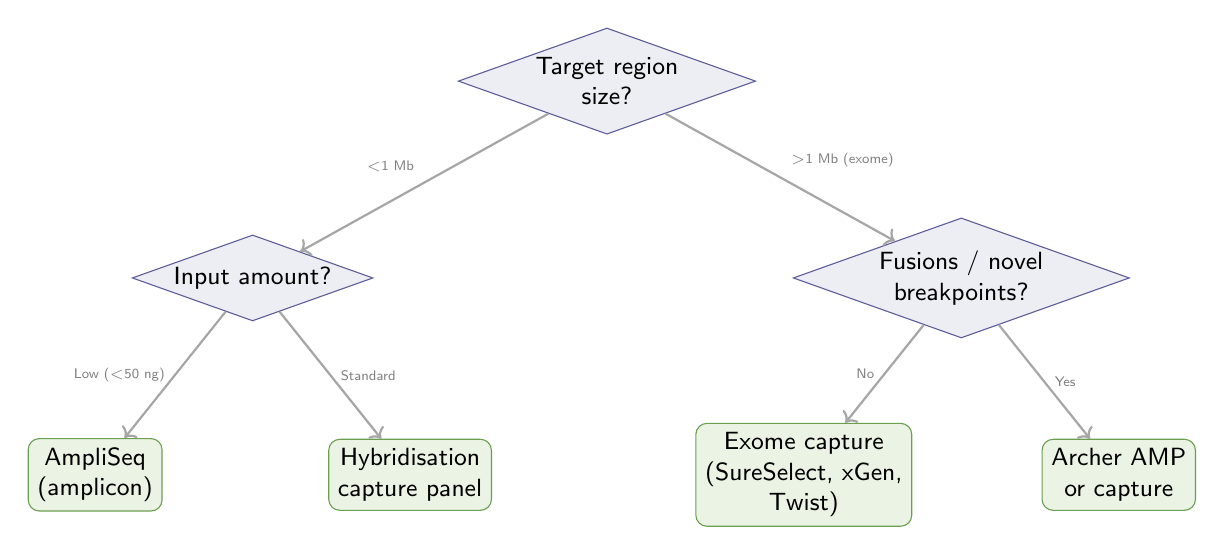
\begin{tikzpicture}[
  decision/.style={diamond, draw=MidnightBlue!70, fill=MidnightBlue!8,
    inner sep=1pt, aspect=2.8, align=center, font=\small\sffamily},
  result/.style={rectangle, draw=OliveGreen!70, fill=OliveGreen!8,
    rounded corners=4pt, minimum height=0.8cm, align=center, font=\small\sffamily},
  arr/.style={->, thick, gray!70},
  lbl/.style={font=\tiny\sffamily, text=gray},
]

\node[decision] (q1) at (0,0) {Target region\\size?};
\node[decision] (q2a) at (-4.5,-2.5) {Input amount?};
\node[decision] (q2b) at (4.5,-2.5) {Fusions / novel\\breakpoints?};

\node[result] (r1) at (-6.5,-5) {AmpliSeq\\(amplicon)};
\node[result] (r2) at (-2.5,-5) {Hybridisation\\capture panel};
\node[result] (r3) at (2.5,-5) {Exome capture\\(SureSelect, xGen,\\Twist)};
\node[result] (r4) at (6.5,-5) {Archer AMP\\or capture};

\draw[arr] (q1) -- node[lbl, above left] {$<$1 Mb} (q2a);
\draw[arr] (q1) -- node[lbl, above right] {$>$1 Mb (exome)} (q2b);
\draw[arr] (q2a) -- node[lbl, left] {Low ($<$50 ng)} (r1);
\draw[arr] (q2a) -- node[lbl, right] {Standard} (r2);
\draw[arr] (q2b) -- node[lbl, left] {No} (r3);
\draw[arr] (q2b) -- node[lbl, right] {Yes} (r4);

\end{tikzpicture}
\caption[Target enrichment decision flowchart]{Decision flowchart for choosing a target enrichment strategy. For small panels with low input, amplicon-based methods are preferred. For exome-scale targets, hybridisation capture is standard. For fusion detection with unknown partners, anchored multiplex PCR (Archer) or capture-based methods are appropriate.}
\label{fig:enrichment_decision}
\end{figure}


\section{Common Failure Modes and Troubleshooting}
\label{sec:troubleshooting}

Library preparation is a multistep biochemical process with many potential points of failure. \Cref{tab:troubleshooting} summarises the most common problems and their solutions.

\begin{table}[htbp]
\centering
\caption[Library preparation troubleshooting guide]{Common library preparation failure modes, their symptoms, likely causes, and solutions.}
\label{tab:troubleshooting}
\small
\renewcommand{\arraystretch}{1.3}
\begin{tabularx}{\textwidth}{@{}>{\raggedright}p{2.5cm} >{\raggedright}p{3cm} >{\raggedright}p{3cm} X@{}}
\toprule
\textbf{Symptom} & \textbf{Likely Cause} & \textbf{Diagnosis} & \textbf{Solution} \\
\midrule
Very low library yield & Degraded input DNA/RNA; failed ligation & Check input on Bioanalyzer; check adapter integrity & Use fresh extraction; verify enzyme activity; increase input \\
\addlinespace
Adapter dimer peak (120--180\basepair) & Excess adapters relative to insert; low-input protocol & Bioanalyzer/TapeStation & Additional SPRI cleanup (0.8$\times$); reduce adapter concentration \\
\addlinespace
Library too large (broad, $>$800\basepair) & Insufficient fragmentation & Bioanalyzer & Increase fragmentation time/energy; repeat with optimised parameters \\
\addlinespace
Library too small ($<$200\basepair) & Over-fragmentation; over-digestion & Bioanalyzer & Reduce fragmentation time/energy; handle DNA more gently \\
\addlinespace
High duplication rate after sequencing & Low library complexity; too many PCR cycles; overloading & Picard MarkDuplicates metrics & Increase input; reduce PCR cycles; use PCR-free protocol \\
\addlinespace
Low \%PF (clusters passing filter) & Overloading; poor library quality & Run metrics & Reduce loading concentration; verify library QC \\
\addlinespace
Index hopping / sample crosstalk & Free adapters on patterned flow cells; combinatorial indexing & Unexpected barcode combinations & Use UDI; clean libraries; pool immediately before loading \\
\addlinespace
Uneven coverage & GC bias from PCR; Tn5 insertion bias & Coverage plots, GC bias analysis & Use PCR-free protocol; switch from tagmentation to mechanical fragmentation \\
\bottomrule
\end{tabularx}
\end{table}


\section{Decision Framework: Choosing a Library Prep Method}
\label{sec:libprep_decision}

The choice of library preparation protocol depends on multiple factors. The following framework provides guidance:

\begin{figure}[htbp]
\centering
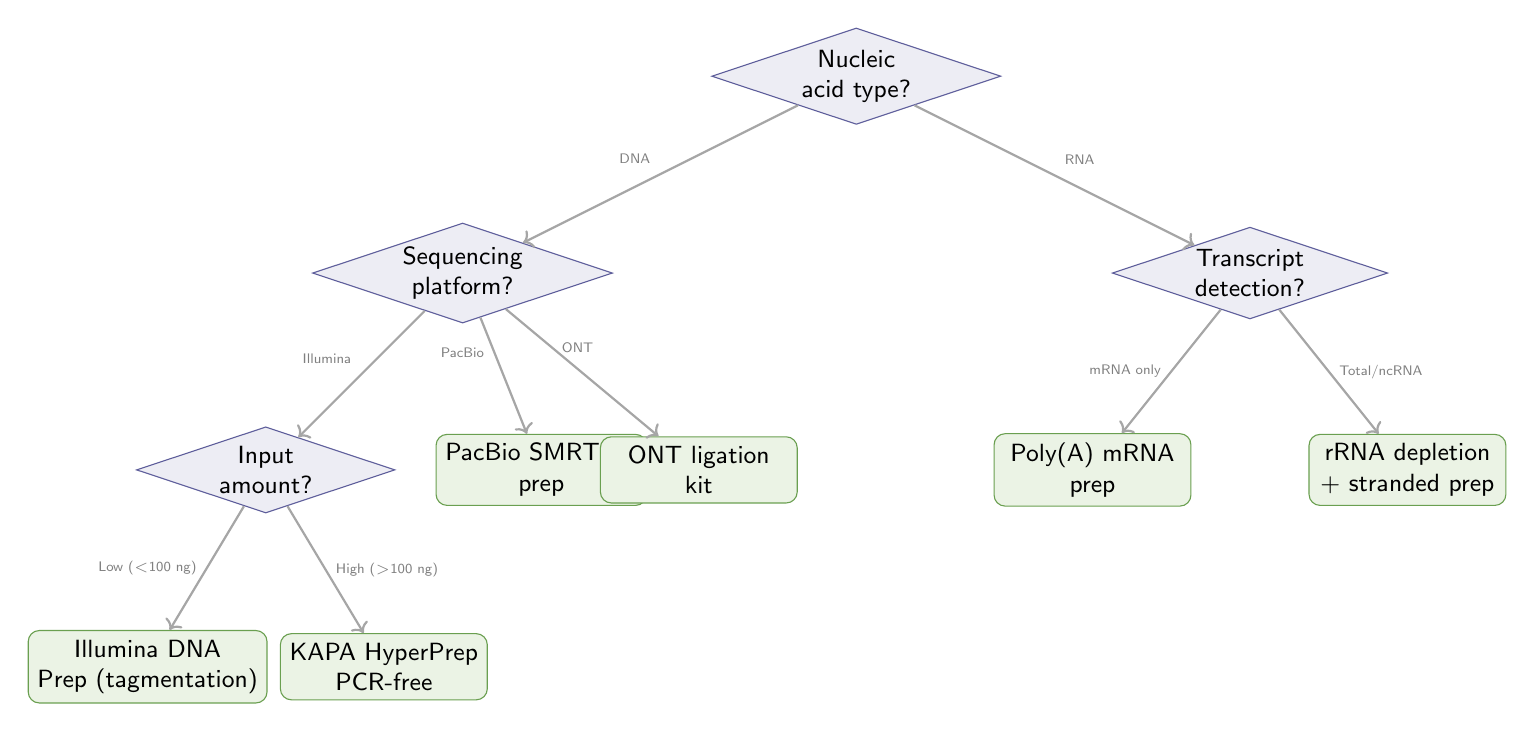
\begin{tikzpicture}[
  decision/.style={diamond, draw=MidnightBlue!70, fill=MidnightBlue!8,
    inner sep=1pt, aspect=3.0, align=center, font=\small\sffamily},
  result/.style={rectangle, draw=OliveGreen!70, fill=OliveGreen!8,
    rounded corners=4pt, minimum width=2.5cm, minimum height=0.7cm, align=center, font=\small\sffamily},
  arr/.style={->, thick, gray!70},
  lbl/.style={font=\tiny\sffamily, text=gray},
]

% Level 1
\node[decision] (q1) at (0,0) {Nucleic\\acid type?};

% Level 2
\node[decision] (q2a) at (-5,-2.5) {Sequencing\\platform?};
\node[decision] (q2b) at (5,-2.5) {Transcript\\detection?};

% Level 3 - DNA branch
\node[decision] (q3a) at (-7.5,-5) {Input\\amount?};
\node[result] (r_pacbio) at (-4,-5) {PacBio SMRTbell\\prep};
\node[result] (r_ont_lig) at (-2,-5) {ONT ligation\\kit};

% Level 3 - RNA branch
\node[result] (r_mrna) at (3,-5) {Poly(A) mRNA\\prep};
\node[result] (r_total) at (7,-5) {rRNA depletion\\+ stranded prep};

% Level 4 - Illumina DNA
\node[result] (r_tagment) at (-9,-7.5) {Illumina DNA\\Prep (tagmentation)};
\node[result] (r_pcr_free) at (-6,-7.5) {KAPA HyperPrep\\PCR-free};

% Arrows
\draw[arr] (q1) -- node[lbl, above left] {DNA} (q2a);
\draw[arr] (q1) -- node[lbl, above right] {RNA} (q2b);

\draw[arr] (q2a) -- node[lbl, above left] {Illumina} (q3a);
\draw[arr] (q2a) -- node[lbl, left, pos=0.3] {PacBio} (r_pacbio);
\draw[arr] (q2a) -- node[lbl, right, pos=0.3] {ONT} (r_ont_lig);

\draw[arr] (q2b) -- node[lbl, left] {mRNA only} (r_mrna);
\draw[arr] (q2b) -- node[lbl, right] {Total/ncRNA} (r_total);

\draw[arr] (q3a) -- node[lbl, left] {Low ($<$100 ng)} (r_tagment);
\draw[arr] (q3a) -- node[lbl, right] {High ($>$100 ng)} (r_pcr_free);

\end{tikzpicture}
\caption[Library preparation decision flowchart]{Decision flowchart for selecting a library preparation method. The primary decision points are the nucleic acid type (DNA vs.\ RNA), the sequencing platform, the available input amount, and the target transcript population.}
\label{fig:libprep_decision}
\end{figure}

\begin{protocolbox}[title={Library Prep Selection Summary}]
\textbf{For Illumina DNA WGS:}
\begin{itemize}[nosep]
  \item High input ($>$100~ng): KAPA HyperPrep PCR-free or Illumina DNA PCR-Free Prep.
  \item Low input ($<$100~ng): Illumina DNA Prep (tagmentation) or NEBNext Ultra~II with PCR.
  \item Ultra-low input / FFPE: NEBNext Ultra~II with increased PCR cycles; consider UMIs.
\end{itemize}

\textbf{For Illumina RNA-seq:}
\begin{itemize}[nosep]
  \item Standard mRNA: Illumina Stranded mRNA Prep or NEBNext Ultra~II RNA.
  \item Total RNA / degraded: rRNA depletion (Ribo-Zero / NEBNext rRNA Depletion) + stranded library prep.
  \item Low input: SMART-Seq (full-length) or NEB Ultra~II RNA (directional).
\end{itemize}

\textbf{For PacBio HiFi:}
\begin{itemize}[nosep]
  \item Standard WGS: SMRTbell prep kit 3.0, targeting 15--20\kilobase\ inserts.
  \item Iso-Seq (full-length transcripts): SMRTbell Iso-Seq Express protocol.
\end{itemize}

\textbf{For ONT:}
\begin{itemize}[nosep]
  \item Maximum read length: Ligation sequencing kit (SQK-LSK114) with UHMW DNA.
  \item Rapid turnaround: Rapid sequencing kit (SQK-RAD114).
  \item Multiplexed: Rapid barcoding kit (SQK-RBK114) or native barcoding kit (SQK-NBD114).
  \item Direct RNA: Direct RNA sequencing kit (SQK-RNA004).
\end{itemize}
\end{protocolbox}


\section{Automation and High-Throughput Library Preparation}
\label{sec:automation}

For core facilities and large-scale projects, manual library preparation is impractical. Liquid-handling robots (e.g., Beckman Coulter Biomek, Hamilton STAR, Opentrons OT-2) can automate most library preparation steps:

\begin{itemize}[nosep]
  \item \textbf{Advantages:} reproducibility, reduced hands-on time, throughput (96 or 384 samples per batch), reduced pipetting errors.
  \item \textbf{Considerations:} requires protocol optimisation for robotic execution (tip types, mixing strategies, magnetic plate timing), significant upfront programming effort, and ongoing maintenance.
  \item \textbf{Common automated workflows:} Illumina DNA Prep on Hamilton, KAPA HyperPrep on Biomek, NEBNext Ultra~II on Opentrons.
\end{itemize}

\begin{tipbox}[title={Starting with Automation}]
If you are new to automated library preparation, start by automating the most time-consuming and error-prone steps (SPRI cleanups, PCR setup, normalisation) while performing fragmentation and adapter ligation manually. Once confident, expand to full protocol automation.
\end{tipbox}


\section{Cost Considerations}
\label{sec:libprep_cost}

Library preparation costs can be a significant component of the overall per-sample sequencing cost, especially for low-throughput applications:

\begin{itemize}[nosep]
  \item \textbf{Standard WGS library:} \$30--100 per sample (depending on kit and protocol).
  \item \textbf{RNA-seq library:} \$50--150 per sample (including RNA extraction and QC).
  \item \textbf{Exome capture:} \$100--200 per sample (library prep + capture probes).
  \item \textbf{10x Genomics single-cell:} \$1{,}500--3{,}000 per run (capturing 5{,}000--10{,}000 cells).
  \item \textbf{ONT rapid sequencing:} \$20--50 per sample (excluding flow cell cost).
\end{itemize}

Bulk purchasing, automation, and protocol miniaturisation (reducing reagent volumes) can substantially reduce per-sample costs for high-throughput operations.


\section{Summary}

Library preparation is the crucial bridge between biological samples and sequencing data. The choice of extraction method, fragmentation approach, adapter chemistry, size selection, amplification strategy, and quality control steps all directly impact data quality and the success of downstream analysis. Key principles to remember:

\begin{enumerate}[nosep]
  \item \textbf{Start with high-quality input.} No library preparation protocol can rescue severely degraded nucleic acid.
  \item \textbf{Minimise PCR.} Use PCR-free protocols when possible; minimise cycle numbers when PCR is necessary.
  \item \textbf{Use appropriate controls.} Include positive controls, negative controls, and PhiX spike-ins.
  \item \textbf{QC rigorously.} Always measure library concentration (Qubit), size distribution (Bioanalyzer/TapeStation), and functional molarity (qPCR) before sequencing.
  \item \textbf{Use UDIs on patterned flow cells.} Prevent index hopping with unique dual indexes.
  \item \textbf{Match the protocol to the question.} The best library preparation method depends on the nucleic acid type, input amount, sequencing platform, and biological question.
  \item \textbf{Document everything.} Record kit lot numbers, input amounts, PCR cycles, and QC results. Library preparation metadata is essential for troubleshooting and reproducibility.
\end{enumerate}

% Part III: DNA Sequencing Applications
\part{Genomics: Reading the Blueprint}
\chapter{Whole-Genome and Exome Sequencing}
\label{ch:genomeseq}

The ability to read the complete DNA sequence of an organism---or strategically selected portions of it---has transformed biology, medicine, and agriculture. In this chapter, we explore the three major strategies for interrogating genomic DNA: \textbf{whole-genome sequencing (WGS)}, which captures every nucleotide from telomere to telomere; \textbf{whole-exome sequencing (WES)}, which focuses on the protein-coding regions; and \textbf{targeted gene panels}, which zoom in on a curated set of genes relevant to a specific clinical question. We examine the technical workflows, compare the trade-offs of each approach, and build complete analysis pipelines in both Snakemake and Nextflow.

%% ============================================================
\section{Whole-Genome Sequencing (WGS)}
\label{sec:wgs}
%% ============================================================

\subsection{What WGS Captures}

Whole-genome sequencing aims to determine the nucleotide sequence of an organism's \emph{entire} genome. For the human genome, this means approximately 3.1 billion base pairs distributed across 22 autosomes and two sex chromosomes, plus the 16.6\kilobase{} mitochondrial genome. Critically, WGS captures:

\begin{itemize}[nosep]
  \item \textbf{Protein-coding exons} ($\sim$1.5\% of the genome, $\sim$20,000 genes).
  \item \textbf{Non-coding regulatory elements}: promoters, enhancers, silencers, insulators, and super-enhancers that control when, where, and how much a gene is expressed.
  \item \textbf{Intronic sequences}: including splice-regulatory elements and deeply intronic variants that can create cryptic exons.
  \item \textbf{Intergenic regions}: harbouring long non-coding RNA (lncRNA) genes, microRNA genes, and disease-associated variants identified by GWAS.
  \item \textbf{Repetitive elements}: transposable elements (SINEs, LINEs, LTRs), tandem repeats (microsatellites, minisatellites), segmental duplications, and centromeric/telomeric satellite DNA.
  \item \textbf{Structural variation}: large deletions, duplications, inversions, and translocations that are invisible to exome-only approaches.
  \item \textbf{Mitochondrial DNA}: enabling studies of heteroplasmy, maternal lineage, and mitochondrial disease.
\end{itemize}

\begin{keyconcept}[title={Why the Non-Coding Genome Matters}]
Although only $\sim$1.5\% of the human genome encodes proteins, the ENCODE project demonstrated that $\sim$80\% shows biochemical activity. Over 90\% of disease-associated variants from GWAS fall in non-coding regions. WGS is the only unbiased approach that captures all of these elements.
\end{keyconcept}

\subsection{When to Use WGS vs.\ Targeted Approaches}

The decision of whether to perform WGS, WES, or a targeted panel depends on the scientific question, budget, required depth, and turnaround time. \Cref{tab:wgs_vs_wes_vs_panel} provides a detailed comparison. In general:

\begin{itemize}[nosep]
  \item \textbf{Use WGS} when you need a comprehensive, unbiased view of the genome---for example, in rare disease cases where WES was negative, cancer whole-genome analysis, structural variant detection, population genomics, or de novo genome assembly.
  \item \textbf{Use WES} when the primary question concerns protein-coding variants, particularly for Mendelian disease diagnostics where cost efficiency matters.
  \item \textbf{Use targeted panels} when a well-defined set of genes is associated with the phenotype (e.g., oncology panels, pharmacogenomics panels) and ultra-deep coverage is required for detecting low-frequency variants.
\end{itemize}

\subsection{Sequencing Depth Requirements}
\label{subsec:depth}

Sequencing depth (also called coverage) is the average number of times each base in the genome is read. The required depth depends on the application:

\begin{itemize}[nosep]
  \item \textbf{Germline variant calling}: 30$\times$ is the community standard for high-confidence SNV and indel detection in diploid genomes. The Genome in a Bottle Consortium validated this threshold extensively.
  \item \textbf{Somatic/cancer sequencing}: 60--100$\times$ for tumor samples (paired with $\sim$30--40$\times$ for the matched normal) to reliably detect subclonal mutations at variant allele frequencies (VAF) as low as 5--10\%.
  \item \textbf{Ultra-deep cancer sequencing}: 500--1000$\times$ or more for detecting rare subclonal variants or circulating tumor DNA (ctDNA) in liquid biopsies.
  \item \textbf{De novo assembly}: 30--50$\times$ HiFi long reads, supplemented by 60--100$\times$ ultra-long Oxford Nanopore reads for scaffolding.
  \item \textbf{Population-scale studies}: As low as 4--10$\times$ with imputation (e.g., the TOPMed and All of Us programs) to reduce per-sample cost while maintaining statistical power at the cohort level.
\end{itemize}

\begin{warningbox}[title={Low-Pass WGS Limitations}]
Low-pass WGS ($<$10$\times$) is cost-effective for large population studies when combined with genotype imputation, but it is \emph{not} suitable for clinical variant calling in individual patients. Individual genotype calls at low depth have high error rates, and rare variants unique to a single individual cannot be imputed.
\end{warningbox}

\subsection{Short-Read WGS Workflow}

The canonical short-read WGS workflow proceeds through the following stages:

\begin{enumerate}[nosep]
  \item \textbf{Library preparation}: Genomic DNA is extracted, fragmented (enzymatic or mechanical), end-repaired, A-tailed, and ligated to platform-specific adapters. PCR amplification (typically 4--8 cycles) or PCR-free protocols are used. PCR-free libraries reduce amplification bias and are preferred for WGS.
  \item \textbf{Sequencing}: Libraries are loaded onto the sequencing instrument (e.g., Illumina NovaSeq X, AVITI by Element Biosciences). Paired-end 150\basepair{} reads are standard for WGS.
  \item \textbf{Quality control}: Raw FASTQ files are assessed with \software{FastQC} and \software{MultiQC}. Adapter trimming and quality filtering are performed with \software{fastp} or \software{Trimmomatic}.
  \item \textbf{Alignment}: Trimmed reads are mapped to the reference genome using \software{BWA-MEM2} (or the original \software{BWA-MEM}) for short reads. The output is a sorted BAM/CRAM file.
  \item \textbf{Duplicate marking}: PCR duplicates are flagged with \software{sambamba markdup}, \software{Picard MarkDuplicates}, or \software{biobambam2}.
  \item \textbf{Base quality score recalibration (BQSR)}: GATK's \software{BaseRecalibrator} adjusts quality scores using known variant sites (dbSNP, Mills indels).
  \item \textbf{Variant calling}: Germline variants are called with \software{GATK HaplotypeCaller} or \software{DeepVariant}. Structural variants are called with \software{Manta}, \software{DELLY}, or \software{Smoove}.
  \item \textbf{Variant filtering and annotation}: Variants are filtered (VQSR or hard filters) and annotated with \software{VEP}, \software{SnpEff}, or \software{ANNOVAR}.
\end{enumerate}

\begin{protocolbox}[title={PCR-Free vs.\ PCR-Based WGS Libraries}]
\textbf{PCR-free libraries} are the gold standard for WGS because they:
\begin{itemize}[nosep]
  \item Eliminate PCR duplicate reads, increasing effective coverage.
  \item Reduce GC-composition bias, improving uniformity across AT-rich and GC-rich regions.
  \item Improve coverage of repetitive regions.
  \item Require higher DNA input ($\sim$100--500\,ng) compared to PCR-based protocols ($\sim$1--50\,ng).
\end{itemize}
Use PCR-based protocols only when input DNA is limiting (e.g., clinical FFPE samples, forensic samples).
\end{protocolbox}

\subsection{Long-Read WGS}

Long-read sequencing technologies from PacBio (HiFi reads, 10--25\kilobase{} at $>$Q30 accuracy) and Oxford Nanopore Technologies (ultra-long reads exceeding 100\kilobase{}, some $>$1\megabase{}) provide critical advantages for WGS:

\begin{itemize}[nosep]
  \item \textbf{Structural variant detection}: Long reads span breakpoints of deletions, duplications, inversions, and translocations that are invisible to short reads due to repetitive flanking sequences.
  \item \textbf{Haplotype phasing}: Reads that span multiple heterozygous variants enable direct physical phasing of alleles across kilobases to megabases.
  \item \textbf{Repeat characterisation}: Tandem repeat expansions (e.g., \gene{FMR1} CGG repeats in Fragile X, \gene{HTT} CAG repeats in Huntington's disease, \gene{C9orf72} GGGGCC repeats in ALS/FTD) can be directly measured.
  \item \textbf{Methylation detection}: Nanopore sequencing natively detects 5-methylcytosine (5mC) and other base modifications without bisulfite conversion.
  \item \textbf{De novo assembly}: Long reads are essential for resolving repetitive regions and producing highly contiguous genome assemblies.
\end{itemize}

\begin{tipbox}[title={Combining Short and Long Reads}]
A hybrid approach using 30$\times$ short-read Illumina data plus 30$\times$ PacBio HiFi data provides the best of both worlds: the cost-effective SNV/indel accuracy of short reads and the structural variant resolution and phasing of long reads. This is increasingly being adopted in clinical rare disease programs.
\end{tipbox}

\subsection{De Novo Genome Assembly}
\label{subsec:denovo}

De novo genome assembly is the process of reconstructing a genome sequence without a reference. This is essential for non-model organisms, population-specific reference construction, and resolving complex genomic regions that collapse in reference-based analyses.

\subsubsection{Assembly Concepts}

\begin{description}[style=nextline]
  \item[Contigs] Contiguous sequences assembled from overlapping reads. A contig has no gaps.
  \item[Scaffolds] Ordered and oriented contigs linked by paired-end or long-range information (mate-pair reads, Hi-C, optical mapping), with gaps represented as stretches of N characters.
  \item[N50] The length $N$ such that 50\% of the total assembly size is contained in contigs (or scaffolds) of length $\geq N$. Higher N50 indicates a more contiguous assembly. Note: N50 alone does not measure \emph{correctness}.
  \item[NG50] Like N50, but normalised to the expected genome size rather than the assembly size. Prevents inflated N50 from incomplete assemblies.
  \item[BUSCO completeness] Benchmarking Universal Single-Copy Orthologs---measures the fraction of expected single-copy genes present in the assembly. A complete genome should have $>$95\% BUSCO completeness.
  \item[QV (consensus quality)] The Phred-scaled accuracy of the consensus sequence. QV50 means one error per 100,000 bases; QV60 means one error per 1,000,000 bases.
\end{description}

\subsubsection{Modern Assembly Approaches}

Current best-practice de novo assembly combines multiple data types:

\begin{enumerate}[nosep]
  \item \textbf{PacBio HiFi assembly}: Tools such as \software{hifiasm} produce highly accurate, haplotype-resolved assemblies from HiFi reads alone.
  \item \textbf{Ultra-long ONT reads}: Reads $>$100\kilobase{} span centromeric satellites, segmental duplications, and other complex repeats. \software{Verkko} and \software{hifiasm} (with ONT integration) use these to connect HiFi contigs.
  \item \textbf{Hi-C scaffolding}: Chromatin conformation data provides chromosome-scale scaffolding. Tools: \software{YaHS}, \software{SALSA2}, \software{3D-DNA}.
  \item \textbf{Polishing}: Consensus accuracy is refined using \software{DeepConsensus} (PacBio), \software{Medaka} (ONT), or short-read polishing with \software{Pilon} or \software{Merqury}-guided assessment.
\end{enumerate}

\subsubsection{De Bruijn Graph Formalism}
\label{subsubsec:genomeseq:debruijn}

Most modern short-read assemblers---including \software{SPAdes}, \software{MEGAHIT}, and the local assembly module within \software{GATK HaplotypeCaller}---are founded on \textbf{de Bruijn graphs}. Understanding this formalism is essential for interpreting assembly behaviour and diagnosing failures.

\begin{keyconcept}[title={Definition of a de Bruijn Graph}]
Given a set of reads and a fixed integer $k$, the de Bruijn graph $G_k = (V, E)$ is a directed graph defined as follows:
\begin{itemize}[nosep]
  \item \textbf{Nodes} $V$: Every unique $(k{-}1)$-mer observed in the read set.
  \item \textbf{Edges} $E$: For each $k$-mer $s_1 s_2 \cdots s_k$ in the reads, a directed edge connects the $(k{-}1)$-mer prefix $s_1 \cdots s_{k-1}$ to the $(k{-}1)$-mer suffix $s_2 \cdots s_k$.
\end{itemize}
The genome reconstruction problem reduces to finding a path through this graph that traverses every \emph{edge} exactly once---an \textbf{Eulerian path}.
\end{keyconcept}

A connected directed graph possesses an Eulerian path if and only if (i) it is connected (considering the underlying undirected graph) and (ii) at most two nodes have unequal in-degree and out-degree. When these conditions hold, the walk can be computed in $O(|E|)$ time using Hierholzer's algorithm. In practice, sequencing errors, polymorphisms, and repeats introduce branches, tips, and bubbles that must be resolved by heuristic graph simplification.

\paragraph{Choice of $k$: the sensitivity--specificity trade-off.}
The parameter $k$ profoundly affects assembly quality:

\begin{itemize}[nosep]
  \item \textbf{Small $k$} increases \emph{sensitivity}: more $k$-mers survive the read error filter, producing a more connected graph. However, many distinct genomic loci share the same short $k$-mer, collapsing repeats and creating ambiguous paths.
  \item \textbf{Large $k$} increases \emph{specificity}: $k$-mers are more likely to be unique in the genome, resolving repeats and reducing spurious edges. However, $k$-mers that span sequencing errors are lost, fragmenting the graph.
\end{itemize}

The number of distinct $k$-mers in a genome of size $G$ is bounded by:
\begin{equation}
\label{eq:genomeseq:kmers}
N_k \leq \min\!\bigl(G - k + 1,\; 4^k\bigr),
\end{equation}
where $4^k$ is the total number of possible $k$-mers over the DNA alphabet $\{A,C,G,T\}$. For the human genome ($G \approx 3.1 \times 10^9$), $k = 17$ yields $4^{17} \approx 1.7 \times 10^{10} > G$, so most 17-mers are unique; for $k = 11$, $4^{11} \approx 4.2 \times 10^6 \ll G$, meaning extensive $k$-mer collisions are inevitable. Multi-$k$ assemblers (e.g., \software{SPAdes}) iteratively build graphs at increasing $k$ values to combine the connectivity of small $k$ with the specificity of large $k$.

\begin{tipbox}[title={Practical $k$-mer Selection Rules}]
For Illumina 150\basepair{} paired-end data, $k$ values in the range 21--77 are typical. As a rule of thumb, $k$ should be (i) odd (to avoid palindromic $k$-mers), (ii) shorter than the read length, and (iii) large enough that $4^k \gg G$. Tools such as \software{KMC3} and \software{Jellyfish2} enable rapid $k$-mer counting to assess the $k$-mer spectrum before assembly.
\end{tipbox}

\paragraph{Repeat resolution strategies.}
Repeats longer than $k - 1$ bases collapse into the same graph path, creating ambiguity. Several strategies address this:

\begin{itemize}[nosep]
  \item \textbf{Paired-end information}: Mate-pair or paired-end reads spanning a repeat connect the flanking unique sequences, enabling the assembler to thread through the correct path.
  \item \textbf{Read clouds / linked reads}: Barcoded short reads from the same long DNA molecule (10x Genomics Chromium, TELL-Seq, stLFR) provide long-range linkage without long-read sequencing.
  \item \textbf{Long reads}: HiFi and ultra-long ONT reads span most genomic repeats outright, enabling overlap-layout-consensus (OLC) or string-graph assembly that avoids the de Bruijn $k$-mer limitation entirely.
  \item \textbf{Coverage depth}: Unique regions have single-copy coverage, whereas collapsed repeats exhibit proportionally elevated coverage. Assemblers exploit this signal to estimate repeat copy number.
\end{itemize}

\subsubsection{Assembly Quality Metrics: Formal Definitions}
\label{subsubsec:genomeseq:assembly_metrics}

While N50 and NG50 were introduced informally above, their precise mathematical definitions are essential for rigorous benchmarking.

Let an assembly consist of $n$ contigs with lengths $l_1 \geq l_2 \geq \cdots \geq l_n$, and let $G$ denote the known or estimated genome size.

\begin{description}[style=nextline]
  \item[N50] The contig length $L$ such that the sum of lengths of all contigs with $l_i \geq L$ constitutes at least half the total assembly size:
    \begin{equation}
    \label{eq:genomeseq:n50}
    \text{N50} = L \quad \text{where} \quad \sum_{i:\, l_i \geq L} l_i \;\geq\; \frac{1}{2}\sum_{j=1}^{n} l_j.
    \end{equation}
  \item[NG50] Identical to N50, but the denominator is the expected genome size $G$ rather than the assembly size:
    \begin{equation}
    \label{eq:genomeseq:ng50}
    \text{NG50} = L \quad \text{where} \quad \sum_{i:\, l_i \geq L} l_i \;\geq\; \frac{G}{2}.
    \end{equation}
    NG50 penalises incomplete assemblies, which may have artificially inflated N50 values.
  \item[auN (area under the Nx curve)] A single statistic that captures the entire contiguity distribution rather than a single percentile. It is defined as:
    \begin{equation}
    \label{eq:genomeseq:aun}
    \mathrm{auN} = \frac{\sum_{i=1}^{n} l_i^2}{\sum_{i=1}^{n} l_i} = \frac{\sum_{i=1}^{n} l_i^2}{A},
    \end{equation}
    where $A = \sum_i l_i$ is the total assembly length. Intuitively, auN is the expected contig length at a randomly chosen assembled base. It avoids the arbitrariness of the 50\% threshold and is increasingly preferred for benchmarking.
\end{description}

\begin{warningbox}[title={Contiguity Is Not Correctness}]
N50, NG50, and auN measure \emph{contiguity} only. A highly contiguous but mis-assembled genome (e.g., with chimeric joins) will have inflated metrics. Always complement contiguity statistics with \emph{correctness} metrics: BUSCO completeness, QV estimated by \software{Merqury}, and reference-based mis-assembly counts from \software{QUAST}.
\end{warningbox}

\subsubsection{Scaffolding Algorithms}
\label{subsubsec:genomeseq:scaffolding}

Scaffolding bridges gaps between contigs by ordering and orienting them using long-range linkage information. Three major data types are used:

\begin{description}[style=nextline]
  \item[Hi-C] Chromatin conformation capture generates read pairs from DNA fragments that were spatially proximal in the nucleus. Because contact probability decays as a power law with genomic distance ($P_{\text{contact}} \propto d^{-\gamma}$, with $\gamma \approx 1$ for mammalian genomes), Hi-C links contigs across megabase scales and assigns them to chromosomes. Tools: \software{YaHS}, \software{SALSA2}, \software{3D-DNA}, \software{ALLHiC} (for polyploid genomes).
  \item[Linked reads] Technologies such as 10x Genomics Chromium, TELL-Seq, and stLFR attach a shared barcode to short reads derived from the same $\sim$50--100\kilobase{} DNA molecule. Barcode co-occurrence connects contigs separated by up to $\sim$100\kilobase{}. Tools: \software{scaff10x}, \software{Tigmint} (mis-assembly detection), \software{Arcs}.
  \item[Optical maps] Bionano optical mapping generates restriction-enzyme--site patterns along megabase-length single molecules. These patterns are aligned to assembled contigs, enabling gap sizing and scaffolding across repeats invisible to sequence-based methods. Tools: \software{Bionano Solve}, \software{OMTools}.
\end{description}

\begin{tipbox}[title={Combining Multiple Scaffolding Data Types}]
The highest-contiguity assemblies integrate all available evidence. A common strategy: (1) assemble HiFi reads with \software{hifiasm}, (2) scaffold with linked-read data or ultra-long ONT reads, (3) apply Hi-C scaffolding to achieve chromosome-scale, and (4) validate with optical maps. The VGP (Vertebrate Genomes Project) pipeline exemplifies this multi-layered approach.
\end{tipbox}

\subsection{Telomere-to-Telomere (T2T) Assemblies}

The Telomere-to-Telomere (T2T) Consortium achieved a landmark in 2022 by completing the first gapless human genome assembly, T2T-CHM13. This filled $\sim$200\megabase{} of previously unresolved sequence, including:

\begin{itemize}[nosep]
  \item All 22 autosomal centromeres (arrays of $\alpha$-satellite repeats).
  \item The five acrocentric short arms (chromosomes 13, 14, 15, 21, 22) containing ribosomal DNA arrays.
  \item Telomeric repeats (TTAGGG)$_n$ at all chromosome ends.
  \item Segmental duplications that collapsed in previous assemblies.
  \item 99 previously unannotated protein-coding genes.
\end{itemize}

The T2T assembly was achieved using a combination of PacBio HiFi reads ($\sim$30$\times$), Oxford Nanopore ultra-long reads ($\sim$120$\times$), and Hi-C data, applied to the CHM13 hydatidiform mole cell line (which is nearly homozygous, simplifying assembly).

\begin{keyconcept}[title={The Evolution of Human Reference Genomes}]
\begin{description}[nosep,style=nextline]
  \item[GRCh37/hg19 (2009)] The workhorse reference for a decade. Still used in many legacy clinical databases.
  \item[GRCh38/hg38 (2013)] Improved representation of centromeres, added alternate loci (ALT contigs). The current standard for most clinical and research pipelines.
  \item[T2T-CHM13 (2022)] The first truly complete human genome. No gaps, no unresolved regions. Increasingly adopted for research, but clinical adoption is ongoing.
  \item[Human Pangenome Reference (2023--)] A graph-based reference incorporating genetic diversity from hundreds of individuals. Reduces reference bias and improves variant calling in diverse populations. Built using \software{Minigraph-Cactus} and \software{PGGB}.
\end{description}
\end{keyconcept}

\subsection{Clinical WGS}

WGS has entered clinical practice in several domains:

\begin{itemize}[nosep]
  \item \textbf{Rare disease diagnosis}: WGS achieves diagnostic yields of 25--40\% in previously undiagnosed cases, outperforming WES (which yields $\sim$25--30\%). The improvement comes from detecting non-coding variants, structural variants, and repeat expansions.
  \item \textbf{Pharmacogenomics}: WGS comprehensively genotypes pharmacogenes (CYP2D6, CYP2C19, CYP3A5, DPYD, TPMT, etc.), including complex structural variants like CYP2D6 gene deletions and duplications.
  \item \textbf{Rapid WGS in NICU/PICU}: Ultra-rapid WGS ($<$24 hours from blood draw to diagnosis) has been implemented for critically ill neonates, achieving diagnostic rates of $\sim$30--40\% and changing clinical management in $\sim$70\% of diagnosed cases.
  \item \textbf{Cancer whole-genome sequencing}: Programmes such as the UK's 100,000 Genomes Project and Hartwig Medical Foundation have demonstrated the clinical utility of tumor/normal WGS for treatment selection.
\end{itemize}

%% ============================================================
\section{Whole-Exome Sequencing (WES)}
\label{sec:wes}
%% ============================================================

\subsection{What the Exome Is}

The exome comprises the protein-coding regions (exons) of all known genes. In the human genome:

\begin{itemize}[nosep]
  \item There are approximately 20,000 protein-coding genes.
  \item The total target region is approximately 30--60\megabase{}, depending on the capture kit and whether UTRs (untranslated regions) and miRNA genes are included.
  \item This represents roughly 1--2\% of the total genome.
  \item Despite its small size, the exome harbours approximately 85\% of known disease-causing mutations (as catalogued in ClinVar and HGMD).
\end{itemize}

\subsection{Hybridisation Capture Workflow}

WES uses hybridisation capture (also called hybrid capture or target enrichment) to selectively enrich exonic sequences:

\begin{enumerate}[nosep]
  \item \textbf{Library preparation}: Standard WGS library prep---fragmentation, end-repair, adapter ligation, PCR amplification.
  \item \textbf{Hybridisation}: The library is incubated with biotinylated oligonucleotide probes (baits) complementary to exonic targets. Hybridisation occurs in solution (liquid-phase capture) over 4--16 hours.
  \item \textbf{Capture}: Streptavidin-coated magnetic beads bind the biotinylated probes and their hybridised library fragments. Non-target fragments are washed away.
  \item \textbf{Amplification}: Captured fragments undergo PCR amplification (8--12 cycles) to generate sufficient material for sequencing.
  \item \textbf{Sequencing}: Paired-end 150\basepair{} reads on Illumina platforms, targeting 80--150$\times$ mean coverage on target.
\end{enumerate}

\begin{warningbox}[title={WES Uniformity Challenges}]
Hybridisation capture is inherently non-uniform. Some exons are captured efficiently while others are poorly represented due to:
\begin{itemize}[nosep]
  \item Extreme GC content (very AT-rich or GC-rich regions).
  \item Repetitive sequences flanking target exons.
  \item Pseudogene interference (probes cross-hybridise to homologous pseudogene sequences).
  \item Probe design gaps in newly annotated genes.
\end{itemize}
Typically, 80--90\% of target bases achieve $\geq$20$\times$ coverage, but some clinically important exons may be consistently undercovered.
\end{warningbox}

\subsection{When WES Is Preferred over WGS}

\begin{itemize}[nosep]
  \item \textbf{Cost}: WES costs approximately one-third to one-quarter of WGS, making it attractive for large cohort studies and clinical diagnostics in resource-limited settings.
  \item \textbf{Data volume}: A WES dataset is $\sim$5--8\,GB per sample (vs.\ $\sim$80--120\,GB for 30$\times$ WGS), reducing storage and computational requirements.
  \item \textbf{Interpretation}: Coding variants are more easily interpretable than non-coding variants because the genetic code directly predicts amino acid changes.
  \item \textbf{Mendelian disease diagnostics}: For disorders with a suspected monogenic coding-region cause, WES has been the first-line test in many clinical genetics laboratories.
\end{itemize}

\subsection{Limitations of WES}

\begin{itemize}[nosep]
  \item Misses non-coding regulatory variants, deep intronic variants, and variants in non-captured UTRs.
  \item Poor detection of structural variants (limited by short insert sizes and non-uniform capture).
  \item Cannot reliably detect repeat expansions (e.g., trinucleotide repeats).
  \item Cannot detect epigenetic modifications.
  \item Capture-dependent biases reduce sensitivity for some exons, particularly in medically important but technically challenging genes (e.g., \gene{GBA}, \gene{SMN1}, \gene{PMS2}).
\end{itemize}

\subsection{Common Capture Kits}

\begin{table}[htbp]
\centering
\caption{Comparison of major exome capture kits.}
\label{tab:capture_kits}
\begin{tabularx}{\textwidth}{@{}lXccc@{}}
\toprule
\textbf{Kit} & \textbf{Probe Type} & \textbf{Target Size} & \textbf{Uniformity} & \textbf{Notable Features} \\
\midrule
Agilent SureSelect V8 & RNA baits & $\sim$67\megabase{} & High & Long RNA probes, extensive UTR coverage \\
IDT xGen Exome V2 & DNA baits & $\sim$34\megabase{} & Very High & Lockdown probes, excellent uniformity \\
Twist Bioscience Exome 2.0 & DNA baits & $\sim$36\megabase{} & Very High & Synthetic biology--derived probes, fast hybridisation \\
Roche KAPA HyperExome & DNA baits & $\sim$43\megabase{} & High & Integrated with KAPA library prep \\
\bottomrule
\end{tabularx}
\end{table}

%% ============================================================
\section{Targeted Sequencing and Gene Panels}
\label{sec:panels}
%% ============================================================

\subsection{Panel Design Strategies}

Two major approaches exist for targeted sequencing:

\begin{description}[style=nextline]
  \item[Amplicon-based panels] Use multiplex PCR to amplify specific target regions. Examples include the Ion AmpliSeq technology and Illumina AmpliSeq. Advantages: rapid, low DNA input ($\sim$10\,ng), simple workflow. Disadvantages: limited target size ($<$500 genes typically), potential allelic dropout at primer sites, PCR artefacts.
  \item[Hybridisation capture--based panels] Similar to WES but with a restricted probe set. Advantages: larger target regions possible, more uniform coverage, better for CNV detection. Disadvantages: longer workflow, higher DNA input required.
\end{description}

\subsection{Clinical Gene Panels}

\begin{itemize}[nosep]
  \item \textbf{Oncology panels}: Comprehensive cancer gene panels (e.g., MSK-IMPACT with 505 genes, FoundationOne CDx with 324 genes) detect somatic mutations, copy number alterations, microsatellite instability, and tumor mutational burden from FFPE tumor tissue.
  \item \textbf{Hereditary cancer panels}: 50--100+ genes associated with hereditary cancer predisposition (e.g., \gene{BRCA1}, \gene{BRCA2}, \gene{TP53}, \gene{MLH1}, \gene{MSH2}).
  \item \textbf{Cardiology panels}: Genes for cardiomyopathies (\gene{MYH7}, \gene{MYBPC3}), arrhythmias (\gene{SCN5A}, \gene{KCNQ1}), aortopathies (\gene{FBN1}, \gene{TGFBR1}).
  \item \textbf{Neurogenetics panels}: Genes for epilepsy, intellectual disability, neuromuscular disorders, hereditary neuropathies.
  \item \textbf{Pharmacogenomics panels}: Targeted genotyping of key pharmacogenes for pre-emptive drug--gene interaction testing.
\end{itemize}

\subsection{Ultra-Deep Sequencing for Low-Frequency Variants}

Gene panels enable sequencing depths of 1,000--10,000$\times$ or more, which is essential for:

\begin{itemize}[nosep]
  \item Detecting somatic mutations at low VAF in heterogeneous tumors or circulating tumor DNA.
  \item Monitoring minimal residual disease (MRD) after cancer treatment.
  \item Detecting mosaic variants in genetic disorders.
  \item Identifying resistance mutations in infectious disease (e.g., HIV drug resistance, tuberculosis).
\end{itemize}

\begin{tipbox}[title={Unique Molecular Identifiers (UMIs)}]
When sequencing at ultra-high depth, PCR duplicates become a major source of error. UMIs---random oligonucleotide barcodes ligated to each original DNA molecule before amplification---allow computational identification and removal of PCR duplicates, enabling accurate consensus calling from original molecules. Tools such as \software{fgbio} and \software{UMI-tools} handle UMI-aware processing.
\end{tipbox}

%% ============================================================
\section{Reduced Representation Genotyping: RADseq and GBS}
\label{sec:radseq-gbs}
%% ============================================================

Whole-genome sequencing of every individual in a large population study is often prohibitively expensive. \textbf{Reduced representation sequencing} offers a powerful alternative: by restricting sequencing to a reproducible subset of the genome anchored at restriction-enzyme cut sites, researchers can genotype thousands of single nucleotide polymorphisms (SNPs) across hundreds or thousands of individuals at a fraction of the cost of WGS. Two dominant approaches are \textbf{Restriction site Associated DNA sequencing (RADseq)} and \textbf{Genotyping by Sequencing (GBS)}.

\subsection{The Core Principle}
\label{subsec:radseq:principle}

Both approaches exploit restriction endonucleases to fragment genomic DNA at predictable, sequence-specific positions. Because the same enzyme cuts the same positions across all individuals of a species, sequencing reads from different samples align to the same genomic loci, enabling comparative SNP genotyping without a prior SNP array or fully sequenced reference genome (though a reference improves analysis considerably).

The fraction of the genome sampled is controlled by enzyme choice:
\begin{itemize}[nosep]
  \item \textbf{Rare cutters} (6--8\,bp recognition sequences, e.g., \textit{SbfI}, \textit{EcoRI}) produce fewer, larger fragments and are suited to large genomes or when fewer, high-coverage loci are desired.
  \item \textbf{Frequent cutters} (4\,bp recognition sequences, e.g., \textit{MseI}, \textit{MspI}) produce more fragments, increasing genome coverage but also sequencing costs per sample.
  \item \textbf{Methylation-sensitive enzymes} (e.g., \textit{PstI} in GBS) preferentially cut in low-methylation, gene-rich regions, enriching for functionally relevant loci while reducing repetitive element contamination.
\end{itemize}

\subsection{RADseq Protocol Variants}
\label{subsec:radseq:variants}

\begin{description}[style=nextline]
  \item[Original RADseq] Digest genomic DNA with a single restriction enzyme, ligate P1 adapters containing a sample-specific barcode, randomly shear with Covaris, size-select fragments ($\sim$300--600\,bp), ligate P2 adapters, and PCR-amplify. Reads originate from one side of each restriction site. Introduced by Miller et al. (2007) and popularised by Baird et al. (2008).

  \item[Double-digest RADseq (ddRAD)] Use two restriction enzymes (one rare cutter + one common cutter) rather than random shearing to define fragment size. This is more reproducible, cheaper, and avoids sonication artefacts. The enzyme pair determines the fraction of the genome sampled. ddRAD has become one of the most widely used approaches.

  \item[2b-RAD] Uses Type IIB restriction enzymes (e.g., \textit{BsaXI}) that cut both strands at a defined distance from their recognition site, producing uniform 36\,bp fragments. All loci are represented at equal depth, simplifying analysis.

  \item[ezRAD] Replaces P1 adapter ligation with random-primed amplification; requires only commercially available Illumina library prep kits and is accessible to labs without molecular biology expertise.

  \item[rapture (RADcap)] Combines RADseq library preparation with hybridisation capture to target a defined subset of RAD loci across thousands of individuals. Enables consistent SNP panels across very large cohorts at reduced cost.
\end{description}

\subsection{Genotyping by Sequencing (GBS)}
\label{subsec:gbs}

Developed by Elshire et al. (2011) at Cornell University, \textbf{GBS} simplifies the RADseq protocol by eliminating the random shearing and size-selection steps. Genomic DNA is digested with one or two restriction enzymes (commonly \textit{ApeKI} or the two-enzyme combination \textit{EcoRI}+\textit{MspI}), and adapters are ligated directly to the sticky ends. All fragments are then PCR-amplified and sequenced. GBS is extremely simple to perform, requires only $\sim$100\,ng input DNA, and can process 96--384 samples per lane of sequencing.

\begin{warningbox}[title={GBS vs RADseq: Missing Data}]
GBS's simplicity comes at a cost: because no size selection is performed, fragment sizes are highly variable, leading to uneven locus representation and substantial missing data (loci with no reads in a given sample). Downstream analysis must account for missing genotypes. RADseq variants with size selection (ddRAD, 2b-RAD) achieve more consistent coverage across samples.
\end{warningbox}

\subsubsection{Two-Enzyme GBS}
Using two enzymes (\textit{EcoRI} + \textit{MspI}) in a double-digest GBS design enriches for fragments flanked by one cut site from each enzyme on opposite ends, reducing the total number of sequenced loci to a more manageable set and decreasing the proportion of repetitive elements.

\subsection{Applications}
\label{subsec:radseq:applications}

RADseq and GBS have transformed population genomics and breeding:

\begin{itemize}[itemsep=3pt]
  \item \textbf{Population structure and demographic history} in wild populations (fish, birds, insects, plants), including species with no reference genome, using tools such as \software{Stacks} and \software{ipyrad}.
  \item \textbf{Landscape genomics:} correlating allele frequencies with environmental variables (elevation, temperature, precipitation) to identify loci under local adaptation.
  \item \textbf{Phylogenomics:} reconstructing species trees from thousands of loci across divergent taxa, replacing morphological or mitochondrial markers.
  \item \textbf{Quantitative trait locus (QTL) mapping} and genome-wide association studies (GWAS) in crops, livestock, and aquaculture species, where cost per sample is paramount.
  \item \textbf{Conservation genetics:} assessing genetic diversity and inbreeding in threatened or endangered populations.
  \item \textbf{Marker-assisted selection (MAS) in plant breeding:} SNP arrays derived from GBS enable genomic selection models predicting agronomic traits from genotype data alone.
\end{itemize}

\subsection{Bioinformatics Pipeline}
\label{subsec:radseq:bioinformatics}

The canonical RADseq analysis pipeline proceeds as follows:

\begin{enumerate}[nosep]
  \item \textbf{Demultiplexing:} Assign reads to samples by barcode. \software{process\_radtags} (Stacks) or \software{cutadapt} with inline barcode handling.
  \item \textbf{Quality trimming:} Remove adapter sequence and low-quality bases. \software{Trim Galore}, \software{fastp}.
  \item \textbf{Alignment (reference-based):} Align trimmed reads to the reference genome with \software{BWA-MEM} or \software{Bowtie2}.
  \item \textbf{Genotyping:}
    \begin{itemize}[nosep]
      \item Reference-based: \software{Stacks} (\texttt{ref\_map.pl}), \software{GATK HaplotypeCaller}, \software{FreeBayes}.
      \item \textit{De novo} (no reference): \software{Stacks} (\texttt{denovo\_map.pl}) or \software{ipyrad} cluster loci across samples by sequence similarity.
    \end{itemize}
  \item \textbf{SNP filtering:} Filter by minimum allele frequency (MAF $>$0.05), minimum coverage per locus, maximum missing data ($<$50\%), and Hardy--Weinberg equilibrium.
  \item \textbf{Downstream analysis:} \software{PLINK}, \software{ADMIXTURE}, \software{TreeMix}, \software{BayPass}, \software{OutFLANK} for population structure, admixture, gene flow, and selection scan analyses.
\end{enumerate}

\begin{table}[htbp]
\centering
\caption{Comparison of reduced representation genotyping approaches.}
\label{tab:radseq_comparison}
\small
\begin{tabularx}{\textwidth}{@{}l *{5}{>{\raggedright\arraybackslash}X}@{}}
\toprule
\textbf{Feature} & \textbf{RADseq} & \textbf{ddRAD} & \textbf{2b-RAD} & \textbf{GBS} & \textbf{rapture} \\
\midrule
Enzymes & 1 & 2 & Type IIB & 1--2 & 1--2 \\
Size selection & Yes & Yes & No (uniform) & No & Yes \\
Fragment uniformity & Moderate & High & Very high & Low & High \\
Missing data & Low & Low & Low & High & Very low \\
Protocol complexity & Moderate & Moderate & Low & Low & High \\
Loci per sample & 5K--100K & 5K--200K & 5K--50K & 5K--500K & 100--50K \\
Typical input DNA & 1\,\textmu g & 0.5--1\,\textmu g & 0.5\,\textmu g & 100\,ng & 0.5\,\textmu g \\
Cost per sample & \$\$\$ & \$\$ & \$\$ & \$ & \$\$ \\
Best for & Pop. genomics & Pop. genomics & Uniform depth & Agriculture & Large cohorts \\
\bottomrule
\end{tabularx}
\end{table}

\begin{tipbox}[title={Choosing Between RADseq and GBS}]
For population genomics with a reference genome and moderate sample sizes ($<$500), \textbf{ddRAD} offers the best balance of missing data control and protocol simplicity. For plant/animal breeding with very large sample sizes and budget constraints, \textbf{GBS} minimises per-sample cost. When consistent SNP panels must be maintained across multiple years of breeding, \textbf{rapture} (or a traditional SNP array) ensures locus stability. For organisms with no reference genome, use \software{ipyrad}'s \textit{de novo} clustering with either ddRAD or GBS.
\end{tipbox}

%% ============================================================
\section{Comparison of Approaches}
\label{sec:comparison}
%% ============================================================

\begin{table}[htbp]
\centering
\caption{Comprehensive comparison of WGS, WES, and targeted panel sequencing.}
\label{tab:wgs_vs_wes_vs_panel}
\small
\begin{tabularx}{\textwidth}{@{}l*{3}{>{\raggedright\arraybackslash}X}@{}}
\toprule
\textbf{Feature} & \textbf{WGS} & \textbf{WES} & \textbf{Targeted Panel} \\
\midrule
Target region & Entire genome ($\sim$3.1\gigabase{}) & Exons ($\sim$30--60\megabase{}) & Selected genes ($\sim$0.01--2\megabase{}) \\
\addlinespace
Genome coverage & 100\% & $\sim$1--2\% & $<$0.1\% \\
\addlinespace
Typical depth & 30--60$\times$ & 80--150$\times$ & 500--10,000$\times$ \\
\addlinespace
Data per sample & 80--120\,GB & 5--8\,GB & 0.1--1\,GB \\
\addlinespace
SNV detection & Excellent & Good (exonic only) & Excellent (on-target) \\
\addlinespace
SV detection & Good (esp.\ with long reads) & Poor & Very limited \\
\addlinespace
CNV detection & Good & Moderate & Moderate (capture-based) \\
\addlinespace
Non-coding variants & Yes & No (mostly) & No \\
\addlinespace
Repeat expansions & Yes (long reads) & No & Limited \\
\addlinespace
Cost per sample\fmark{*} & \$\$\$\$ & \$\$ & \$ \\
\addlinespace
Turnaround time & 2--4 weeks & 2--4 weeks & 1--2 weeks \\
\addlinespace
Best for & Comprehensive analysis, research, rare disease, cancer & Mendelian disease, cost-effective coding-region screen & Clinical diagnostics, known gene sets, ultra-deep \\
\bottomrule
\end{tabularx}

\vspace{0.3em}
{\footnotesize \fmark{*} Approximate relative cost as of 2025--2026. Absolute costs continue to decrease.}
\end{table}

%% ============================================================
\section{Visual Comparison: WGS vs.\ WES vs.\ Panel}
\label{sec:tikz_comparison}
%% ============================================================

\begin{figure}[htbp]
\centering
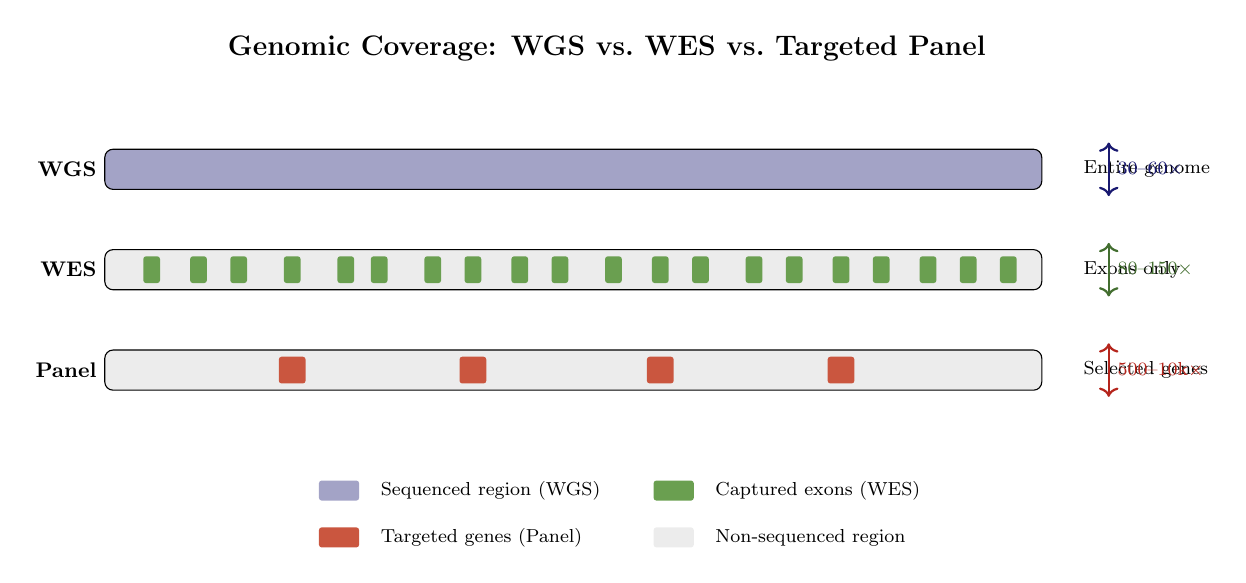
\begin{tikzpicture}[
  scale=0.85,
  transform shape,
  every node/.style={font=\small},
  chrombar/.style={draw, minimum height=0.6cm, rounded corners=3pt, inner sep=0pt},
  exonblock/.style={fill=OliveGreen!70, minimum height=0.4cm, rounded corners=1pt, inner sep=0pt},
  panelblock/.style={fill=BrickRed!70, minimum height=0.4cm, rounded corners=1pt, inner sep=0pt},
  label/.style={font=\small\bfseries, anchor=east},
]

% Title
\node[font=\large\bfseries, anchor=south] at (7, 7.5) {Genomic Coverage: WGS vs.\ WES vs.\ Targeted Panel};

% --- WGS ---
\node[label] at (-0.5, 6) {WGS};
\node[chrombar, fill=MidnightBlue!40, minimum width=14cm] at (6.5, 6) {};
\node[font=\footnotesize, anchor=west] at (14, 6) {Entire genome};

% --- WES ---
\node[label] at (-0.5, 4.5) {WES};
% Background chromosome
\node[chrombar, fill=gray!15, minimum width=14cm] at (6.5, 4.5) {};
% Exons scattered across
\foreach \x in {0.2, 0.9, 1.5, 2.3, 3.1, 3.6, 4.4, 5.0, 5.7, 6.3, 7.1, 7.8, 8.4, 9.2, 9.8, 10.5, 11.1, 11.8, 12.4, 13.0} {
  \node[exonblock, minimum width=0.25cm] at (\x, 4.5) {};
}
\node[font=\footnotesize, anchor=west] at (14, 4.5) {Exons only};

% --- Panel ---
\node[label] at (-0.5, 3) {Panel};
% Background chromosome
\node[chrombar, fill=gray!15, minimum width=14cm] at (6.5, 3) {};
% Only a few targeted genes
\foreach \x in {2.3, 5.0, 7.8, 10.5} {
  \node[panelblock, minimum width=0.4cm] at (\x, 3) {};
}
\node[font=\footnotesize, anchor=west] at (14, 3) {Selected genes};

% Legend
\node[fill=MidnightBlue!40, minimum width=0.6cm, minimum height=0.3cm, rounded corners=1pt] at (3, 1.2) {};
\node[anchor=west, font=\footnotesize] at (3.5, 1.2) {Sequenced region (WGS)};
\node[fill=OliveGreen!70, minimum width=0.6cm, minimum height=0.3cm, rounded corners=1pt] at (8, 1.2) {};
\node[anchor=west, font=\footnotesize] at (8.5, 1.2) {Captured exons (WES)};
\node[fill=BrickRed!70, minimum width=0.6cm, minimum height=0.3cm, rounded corners=1pt] at (3, 0.5) {};
\node[anchor=west, font=\footnotesize] at (3.5, 0.5) {Targeted genes (Panel)};
\node[fill=gray!15, minimum width=0.6cm, minimum height=0.3cm, rounded corners=1pt] at (8, 0.5) {};
\node[anchor=west, font=\footnotesize] at (8.5, 0.5) {Non-sequenced region};

% Depth annotations
\draw[<->, thick, MidnightBlue] (14.5, 5.6) -- (14.5, 6.4) node[midway, right, font=\footnotesize] {30--60$\times$};
\draw[<->, thick, OliveGreen!80!black] (14.5, 4.1) -- (14.5, 4.9) node[midway, right, font=\footnotesize] {80--150$\times$};
\draw[<->, thick, BrickRed] (14.5, 2.6) -- (14.5, 3.4) node[midway, right, font=\footnotesize] {500--10k$\times$};

\end{tikzpicture}
\caption{Visual comparison of genomic coverage achieved by whole-genome sequencing, whole-exome sequencing, and targeted gene panels. WGS covers the entire genome at moderate depth; WES selectively captures exonic regions at higher depth; targeted panels focus on a small gene set at very high depth.}
\label{fig:wgs_wes_panel}
\end{figure}

%% ============================================================
\section{Practical Bioinformatics: WGS Analysis Pipelines}
\label{sec:wgs_pipeline}
%% ============================================================

In this section, we build a complete WGS germline variant calling pipeline in both Snakemake and Nextflow. The workflow follows the best-practice GATK pipeline: quality control with \software{FastQC}, read trimming with \software{fastp}, alignment with \software{BWA-MEM2}, duplicate marking with \software{sambamba}, base quality score recalibration with \software{GATK}, variant calling with both \software{GATK HaplotypeCaller} and \software{DeepVariant}, and variant filtering.

\subsection{Snakemake WGS Pipeline}

\begin{lstlisting}[language=Python, caption={Complete Snakemake WGS germline variant calling pipeline.}, label={lst:snakemake_wgs}]
# Snakefile for WGS Germline Variant Calling Pipeline
# Follows GATK Best Practices

configfile: "config.yaml"

SAMPLES = config["samples"]
REF = config["reference"]
KNOWN_SITES = config["known_sites"]  # dbSNP, Mills indels

rule all:
    input:
        expand("results/vcf/{sample}.filtered.vcf.gz", sample=SAMPLES),
        expand("results/deepvariant/{sample}.dv.vcf.gz", sample=SAMPLES),
        "results/multiqc/multiqc_report.html"

rule fastqc:
    input:
        r1="data/fastq/{sample}_R1.fastq.gz",
        r2="data/fastq/{sample}_R2.fastq.gz"
    output:
        html1="results/qc/fastqc/{sample}_R1_fastqc.html",
        html2="results/qc/fastqc/{sample}_R2_fastqc.html",
        zip1="results/qc/fastqc/{sample}_R1_fastqc.zip",
        zip2="results/qc/fastqc/{sample}_R2_fastqc.zip"
    threads: 2
    shell:
        """
        fastqc -t {threads} -o results/qc/fastqc/ \
            {input.r1} {input.r2}
        """

rule fastp_trim:
    input:
        r1="data/fastq/{sample}_R1.fastq.gz",
        r2="data/fastq/{sample}_R2.fastq.gz"
    output:
        r1="results/trimmed/{sample}_R1.trimmed.fastq.gz",
        r2="results/trimmed/{sample}_R2.trimmed.fastq.gz",
        json="results/qc/fastp/{sample}.fastp.json",
        html="results/qc/fastp/{sample}.fastp.html"
    threads: 4
    shell:
        """
        fastp -i {input.r1} -I {input.r2} \
            -o {output.r1} -O {output.r2} \
            --json {output.json} --html {output.html} \
            --qualified_quality_phred 20 \
            --length_required 50 \
            --adapter_sequence auto \
            --thread {threads}
        """

rule bwa_mem2_align:
    input:
        r1="results/trimmed/{sample}_R1.trimmed.fastq.gz",
        r2="results/trimmed/{sample}_R2.trimmed.fastq.gz",
        ref=REF
    output:
        bam="results/aligned/{sample}.sorted.bam"
    params:
        rg="@RG\\tID:{sample}\\tSM:{sample}\\tPL:ILLUMINA\\tLB:lib1"
    threads: 16
    shell:
        """
        bwa-mem2 mem -t {threads} -R '{params.rg}' {input.ref} \
            {input.r1} {input.r2} \
        | samtools sort -@ 4 -o {output.bam} -
        samtools index {output.bam}
        """

rule sambamba_markdup:
    input:
        bam="results/aligned/{sample}.sorted.bam"
    output:
        bam="results/dedup/{sample}.dedup.bam",
        bai="results/dedup/{sample}.dedup.bam.bai"
    threads: 8
    shell:
        """
        sambamba markdup -t {threads} \
            --tmpdir tmp/ \
            {input.bam} {output.bam}
        """

rule gatk_bqsr:
    input:
        bam="results/dedup/{sample}.dedup.bam",
        ref=REF,
        known=KNOWN_SITES
    output:
        table="results/bqsr/{sample}.recal_data.table",
        bam="results/bqsr/{sample}.recal.bam"
    shell:
        """
        gatk BaseRecalibrator \
            -I {input.bam} -R {input.ref} \
            --known-sites {input.known} \
            -O {output.table}

        gatk ApplyBQSR \
            -I {input.bam} -R {input.ref} \
            --bqsr-recal-file {output.table} \
            -O {output.bam}
        """

rule gatk_haplotypecaller:
    input:
        bam="results/bqsr/{sample}.recal.bam",
        ref=REF
    output:
        gvcf="results/gvcf/{sample}.g.vcf.gz"
    threads: 4
    shell:
        """
        gatk HaplotypeCaller \
            -I {input.bam} -R {input.ref} \
            -O {output.gvcf} \
            -ERC GVCF \
            --native-pair-hmm-threads {threads}
        """

rule gatk_genotype:
    input:
        gvcf="results/gvcf/{sample}.g.vcf.gz",
        ref=REF
    output:
        vcf="results/vcf/{sample}.raw.vcf.gz"
    shell:
        """
        gatk GenotypeGVCFs \
            -R {input.ref} \
            -V {input.gvcf} \
            -O {output.vcf}
        """

rule gatk_filter:
    input:
        vcf="results/vcf/{sample}.raw.vcf.gz",
        ref=REF
    output:
        vcf="results/vcf/{sample}.filtered.vcf.gz"
    shell:
        """
        gatk VariantFiltration \
            -R {input.ref} -V {input.vcf} \
            --filter-expression "QD < 2.0" --filter-name "LowQD" \
            --filter-expression "FS > 60.0" --filter-name "StrandBias" \
            --filter-expression "MQ < 40.0" --filter-name "LowMQ" \
            --filter-expression "MQRankSum < -12.5" --filter-name "MQRankSum" \
            --filter-expression "ReadPosRankSum < -8.0" --filter-name "ReadPos" \
            -O {output.vcf}
        """

rule deepvariant:
    input:
        bam="results/dedup/{sample}.dedup.bam",
        ref=REF
    output:
        vcf="results/deepvariant/{sample}.dv.vcf.gz"
    threads: 16
    shell:
        """
        run_deepvariant \
            --model_type=WGS \
            --ref={input.ref} \
            --reads={input.bam} \
            --output_vcf={output.vcf} \
            --num_shards={threads}
        """

rule multiqc:
    input:
        expand("results/qc/fastqc/{sample}_R1_fastqc.zip", sample=SAMPLES),
        expand("results/qc/fastp/{sample}.fastp.json", sample=SAMPLES)
    output:
        "results/multiqc/multiqc_report.html"
    shell:
        """
        multiqc results/qc/ -o results/multiqc/ --force
        """
\end{lstlisting}

\subsection{Nextflow WGS Pipeline}

\begin{lstlisting}[language=Java, caption={Complete Nextflow DSL2 WGS germline variant calling pipeline.}, label={lst:nextflow_wgs}]
#!/usr/bin/env nextflow
nextflow.enable.dsl=2

// Nextflow WGS Germline Variant Calling Pipeline
// Follows GATK Best Practices

params.reads    = "data/fastq/*_{R1,R2}.fastq.gz"
params.ref      = "reference/hg38.fa"
params.known    = "reference/known_sites.vcf.gz"
params.outdir   = "results"

// ---- Processes ----

process FASTQC {
    tag "$sample_id"
    publishDir "${params.outdir}/qc/fastqc", mode: 'copy'
    cpus 2

    input:
    tuple val(sample_id), path(reads)

    output:
    path("*.{html,zip}"), emit: reports

    script:
    """
    fastqc -t ${task.cpus} ${reads}
    """
}

process FASTP {
    tag "$sample_id"
    publishDir "${params.outdir}/trimmed", mode: 'copy'
    cpus 4

    input:
    tuple val(sample_id), path(reads)

    output:
    tuple val(sample_id),
          path("${sample_id}_R{1,2}.trimmed.fastq.gz"),
          emit: trimmed_reads
    path("${sample_id}.fastp.{json,html}"),
          emit: reports

    script:
    """
    fastp -i ${reads[0]} -I ${reads[1]} \
        -o ${sample_id}_R1.trimmed.fastq.gz \
        -O ${sample_id}_R2.trimmed.fastq.gz \
        --json ${sample_id}.fastp.json \
        --html ${sample_id}.fastp.html \
        --qualified_quality_phred 20 \
        --length_required 50 \
        --thread ${task.cpus}
    """
}

process BWA_MEM2 {
    tag "$sample_id"
    publishDir "${params.outdir}/aligned", mode: 'copy'
    cpus 16

    input:
    tuple val(sample_id), path(reads)
    path ref
    path ref_idx  // .fai, .bwt.2bit.64, .amb, .ann, .pac

    output:
    tuple val(sample_id), path("${sample_id}.sorted.bam"),
          path("${sample_id}.sorted.bam.bai"),
          emit: aligned_bam

    script:
    """
    bwa-mem2 mem -t ${task.cpus} \
        -R "@RG\\tID:${sample_id}\\tSM:${sample_id}\\tPL:ILLUMINA\\tLB:lib1" \
        ${ref} ${reads} \
    | samtools sort -@ 4 -o ${sample_id}.sorted.bam -
    samtools index ${sample_id}.sorted.bam
    """
}

process SAMBAMBA_MARKDUP {
    tag "$sample_id"
    publishDir "${params.outdir}/dedup", mode: 'copy'
    cpus 8

    input:
    tuple val(sample_id), path(bam), path(bai)

    output:
    tuple val(sample_id), path("${sample_id}.dedup.bam"),
          path("${sample_id}.dedup.bam.bai"),
          emit: dedup_bam

    script:
    """
    sambamba markdup -t ${task.cpus} ${bam} ${sample_id}.dedup.bam
    """
}

process GATK_BQSR {
    tag "$sample_id"
    publishDir "${params.outdir}/bqsr", mode: 'copy'

    input:
    tuple val(sample_id), path(bam), path(bai)
    path ref
    path ref_fai
    path ref_dict
    path known_sites
    path known_sites_idx

    output:
    tuple val(sample_id), path("${sample_id}.recal.bam"),
          path("${sample_id}.recal.bam.bai"),
          emit: recal_bam

    script:
    """
    gatk BaseRecalibrator \
        -I ${bam} -R ${ref} \
        --known-sites ${known_sites} \
        -O ${sample_id}.recal_data.table

    gatk ApplyBQSR \
        -I ${bam} -R ${ref} \
        --bqsr-recal-file ${sample_id}.recal_data.table \
        -O ${sample_id}.recal.bam

    samtools index ${sample_id}.recal.bam
    """
}

process HAPLOTYPECALLER {
    tag "$sample_id"
    publishDir "${params.outdir}/vcf", mode: 'copy'
    cpus 4

    input:
    tuple val(sample_id), path(bam), path(bai)
    path ref
    path ref_fai
    path ref_dict

    output:
    tuple val(sample_id),
          path("${sample_id}.g.vcf.gz"),
          emit: gvcf

    script:
    """
    gatk HaplotypeCaller \
        -I ${bam} -R ${ref} \
        -O ${sample_id}.g.vcf.gz \
        -ERC GVCF \
        --native-pair-hmm-threads ${task.cpus}
    """
}

process DEEPVARIANT {
    tag "$sample_id"
    publishDir "${params.outdir}/deepvariant", mode: 'copy'
    cpus 16

    input:
    tuple val(sample_id), path(bam), path(bai)
    path ref
    path ref_fai

    output:
    tuple val(sample_id),
          path("${sample_id}.dv.vcf.gz"),
          emit: dv_vcf

    script:
    """
    run_deepvariant \
        --model_type=WGS \
        --ref=${ref} \
        --reads=${bam} \
        --output_vcf=${sample_id}.dv.vcf.gz \
        --num_shards=${task.cpus}
    """
}

process MULTIQC {
    publishDir "${params.outdir}/multiqc", mode: 'copy'

    input:
    path(reports)

    output:
    path("multiqc_report.html")

    script:
    """
    multiqc . -o . --force
    """
}

// ---- Workflow ----

workflow {
    // Create read-pair channel
    Channel
        .fromFilePairs(params.reads)
        .set { read_pairs_ch }

    ref          = file(params.ref)
    ref_fai      = file("${params.ref}.fai")
    ref_dict     = file(params.ref.replaceAll('.fa$', '.dict'))
    ref_idx      = Channel.fromPath("${params.ref}.*").collect()
    known_sites  = file(params.known)
    known_idx    = file("${params.known}.tbi")

    // Step 1: QC and trimming (in parallel)
    FASTQC(read_pairs_ch)
    FASTP(read_pairs_ch)

    // Step 2: Alignment
    BWA_MEM2(FASTP.out.trimmed_reads, ref, ref_idx)

    // Step 3: Duplicate marking
    SAMBAMBA_MARKDUP(BWA_MEM2.out.aligned_bam)

    // Step 4: BQSR
    GATK_BQSR(SAMBAMBA_MARKDUP.out.dedup_bam,
              ref, ref_fai, ref_dict,
              known_sites, known_idx)

    // Step 5: Variant calling (two callers in parallel)
    HAPLOTYPECALLER(GATK_BQSR.out.recal_bam,
                    ref, ref_fai, ref_dict)
    DEEPVARIANT(SAMBAMBA_MARKDUP.out.dedup_bam,
                ref, ref_fai)

    // Step 6: MultiQC report
    MULTIQC(
        FASTQC.out.reports
            .mix(FASTP.out.reports)
            .collect()
    )
}
\end{lstlisting}

\begin{tipbox}[title={Choosing Between Snakemake and Nextflow}]
Both workflow managers are widely used in genomics. Key considerations:
\begin{itemize}[nosep]
  \item \textbf{Snakemake}: Python-based, file-centric (rules define input/output files), integrates with Conda environments natively, excellent for bioinformaticians comfortable with Python.
  \item \textbf{Nextflow}: Groovy/Java-based, dataflow-driven (channels pass data between processes), strong Docker/Singularity integration, excellent for cloud-native and HPC deployments.
  \item \textbf{nf-core}: A community-curated collection of Nextflow pipelines. The \software{nf-core/sarek} pipeline implements a production-grade WGS/WES variant calling workflow with extensive QC and reporting.
\end{itemize}
\end{tipbox}

%% ============================================================
\section{Long-Read Alignment and Assembly Workflow}
\label{sec:longread_workflow}
%% ============================================================

For long-read WGS data, the alignment and variant calling tools differ:

\begin{itemize}[nosep]
  \item \textbf{Alignment}: \software{minimap2} with preset \texttt{-ax map-hifi} for PacBio HiFi or \texttt{-ax map-ont} for Oxford Nanopore.
  \item \textbf{Small variant calling}: \software{DeepVariant} (PacBio model or ONT model), \software{PEPPER-Margin-DeepVariant} for ONT, \software{Clair3}.
  \item \textbf{Structural variant calling}: \software{pbsv} (PacBio), \software{Sniffles2} (any long reads), \software{cuteSV}, \software{SVIM}.
  \item \textbf{Phasing}: \software{WhatsHap} for read-backed phasing, \software{HiPhase} for PacBio, \software{SHAPEIT5} for statistical phasing at population scale.
  \item \textbf{De novo assembly}: \software{hifiasm} for HiFi reads; \software{Verkko} for HiFi + ONT ultra-long; \software{Flye} for ONT-only assemblies.
  \item \textbf{Methylation}: \software{modkit} (PacBio), \software{modbam2bed} and \software{modkit} (ONT) for extracting base modification information.
\end{itemize}

%% ============================================================
\section{Quality Control Metrics for WGS/WES}
\label{sec:qc_metrics}
%% ============================================================

After alignment and before variant calling, it is essential to assess data quality. Key metrics include:

\begin{table}[htbp]
\centering
\caption{Essential QC metrics for WGS and WES data.}
\label{tab:qc_metrics}
\begin{tabularx}{\textwidth}{@{}lXl@{}}
\toprule
\textbf{Metric} & \textbf{Description} & \textbf{Typical Threshold} \\
\midrule
Mean coverage & Average number of reads covering each base & $\geq$30$\times$ (WGS) \\
\% bases $\geq$20$\times$ & Uniformity of coverage & $\geq$90\% \\
\% mapped reads & Fraction of reads aligning to reference & $\geq$95\% \\
\% properly paired & Fraction of read pairs with concordant alignment & $\geq$90\% \\
\% duplicate reads & PCR duplicate rate & $<$15\% (PCR-free: $<$5\%) \\
Insert size & Fragment length distribution (peak and spread) & 300--500\basepair{} \\
GC bias & Deviation of coverage across GC content bins & Minimal deviation \\
Contamination & Cross-sample contamination (VerifyBamID) & $<$1\% \\
Chimeric reads & Fraction of supplementary/split alignments & $<$5\% \\
On-target rate (WES) & Fraction of reads on capture target & $\geq$70\% \\
\bottomrule
\end{tabularx}
\end{table}

Tools for collecting these metrics include \software{samtools stats}, \software{Picard CollectWgsMetrics}, \software{Picard CollectHsMetrics} (for WES), \software{mosdepth} (fast coverage calculation), and \software{VerifyBamID2} (contamination estimation).

%% ============================================================
\section{Summary}
\label{sec:ch07_summary}
%% ============================================================

\begin{keyconcept}[title={Chapter Summary}]
\begin{itemize}[nosep]
  \item \textbf{WGS} captures the entire genome including coding, non-coding, regulatory, and repetitive regions. It is the most comprehensive but most expensive approach, requiring 30$\times$ for germline and 60--100$\times$ for somatic applications.
  \item \textbf{WES} captures $\sim$1--2\% of the genome (protein-coding exons) at a fraction of the cost of WGS. It is the workhorse for Mendelian disease diagnostics but misses non-coding and structural variants.
  \item \textbf{Targeted panels} offer ultra-deep sequencing of curated gene sets, ideal for clinical diagnostics with well-defined genetic targets.
  \item \textbf{Long-read WGS} (PacBio HiFi, Oxford Nanopore) enables structural variant detection, repeat characterisation, haplotype phasing, and de novo assembly---capabilities that are limited or absent with short reads alone.
  \item The \textbf{T2T-CHM13} assembly and emerging \textbf{pangenome references} are transforming how we represent and analyse human genetic variation.
  \item Both \textbf{Snakemake} and \textbf{Nextflow} provide robust frameworks for building reproducible WGS/WES analysis pipelines, with community-curated pipelines (e.g., \software{nf-core/sarek}) available for immediate use.
\end{itemize}
\end{keyconcept}

\chapter{Variant Discovery and Interpretation}
\label{ch:variants}

\begin{sourcebox}
The computational framework and clinical classification discussion are anchored by the GATK framework and ACMG/AMP consensus guideline \cite{depristo2011,richards2015}. These sources do not make a teaching workflow clinically validated, and later ClinGen refinements and disease-specific specifications may alter evidence use.
\end{sourcebox}

Every human genome carries approximately 4--5 million genetic variants relative to the reference sequence. The vast majority are benign polymorphisms inherited from our ancestors, but a small fraction can cause disease, influence drug response, or drive cancer. Identifying these variants from sequencing data---and distinguishing the pathogenic needles from the benign haystack---is one of the central challenges of modern genomics. This chapter provides a comprehensive treatment of variant types, calling algorithms, quality control, annotation, and clinical interpretation, with practical pipeline examples in both Snakemake and Nextflow.

%% ============================================================
\section{Types of Genetic Variants}
\label{sec:variant_types}
%% ============================================================

Genetic variants span a wide size range, from single nucleotide changes to chromosome-scale rearrangements. Understanding this spectrum is essential for selecting appropriate detection methods.

\subsection{Single Nucleotide Variants (SNVs) and Single Nucleotide Polymorphisms (SNPs)}

An SNV is a change of a single nucleotide at a specific genomic position. A \textbf{single nucleotide polymorphism (SNP)} is an SNV treated as polymorphic in a population; although a 1\% minor-allele-frequency threshold is historically common, nomenclature and database usage do not apply that cutoff uniformly. SNVs are the most abundant variant class: a typical human genome contains millions relative to a reference, with the exact count depending on ancestry, reference assembly, callable regions, and filtering.

SNVs in coding regions are classified by their effect on the encoded protein:
\begin{description}[nosep]
  \item[Synonymous (silent)] The nucleotide change does not alter the amino acid due to codon degeneracy.
  \item[Missense] The change results in a different amino acid.
  \item[Nonsense] The change creates a premature stop codon, truncating the protein.
  \item[Splice-site] The change disrupts a canonical splice donor (GT) or acceptor (AG) site, altering mRNA splicing.
\end{description}

\subsection{Insertions and Deletions (Indels)}

Indels are small insertions or deletions, typically defined as 1--50\basepair{} in length. A typical human genome contains $\sim$500,000--600,000 indels. Indels in coding regions can be:

\begin{description}[nosep]
  \item[Frameshift] The insertion or deletion length is not a multiple of 3, shifting the reading frame of all downstream codons. Usually severely disruptive.
  \item[In-frame] The length is a multiple of 3, adding or removing one or more amino acids without disrupting the reading frame.
\end{description}

\begin{warningbox}[title={Indel Representation Ambiguity}]
Indels in repetitive regions can be represented at multiple equivalent positions (left-aligned vs.\ right-aligned). This ``indel normalisation'' problem can cause the same biological variant to appear as different VCF records. Always use \software{bcftools norm} or \software{vt normalize} to left-align and trim indels before comparison or annotation. This is particularly critical when merging call sets from different tools.
\end{warningbox}

\subsection{Structural Variants (SVs)}

Structural variants are genomic rearrangements typically defined as $>$50\basepair{}. They affect more total bases per genome than SNVs and indels combined. Major SV classes include:

\begin{description}[style=nextline]
  \item[Deletions] Loss of a genomic segment. Detected as reduced coverage and discordant read pairs.
  \item[Duplications] Gain of a genomic segment (tandem or dispersed). Tandem duplications appear as increased coverage and characteristic split-read signatures.
  \item[Inversions] A genomic segment is reversed in orientation. Detected by discordant read-pair orientation.
  \item[Translocations] A genomic segment is moved to a different chromosomal location. Can be balanced (no net gain or loss) or unbalanced. Inter-chromosomal translocations are detected by read pairs mapping to different chromosomes.
  \item[Insertions] Novel sequence is inserted at a position. Includes mobile element insertions (Alu, L1, SVA), nuclear mitochondrial insertions (NUMTs), and viral integrations.
\end{description}

A typical human genome contains $\sim$20,000--30,000 structural variants, collectively affecting $\sim$10--20\megabase{} of sequence.

\subsection{Copy Number Variants (CNVs)}

CNVs are a subset of structural variants involving gains or losses of genomic segments, ranging from kilobases to megabases. They are detected through:
\begin{itemize}[nosep]
  \item \textbf{Read-depth analysis}: Increased or decreased coverage relative to the diploid expectation.
  \item \textbf{B-allele frequency (BAF)}: Deviations from the expected 0/0.5/1 pattern at heterozygous sites indicate gains or losses.
  \item \textbf{Split reads and discordant pairs}: Provide breakpoint-level resolution.
\end{itemize}

\subsection{Repeat Expansions}

Short tandem repeats (STRs, also called microsatellites) are arrays of 1--6\basepair{} repeat units. Pathogenic expansions of these repeats cause over 50 neurological and neuromuscular diseases:

\begin{itemize}[nosep]
  \item \gene{HTT}: CAG expansion $>$36 repeats causes Huntington's disease.
  \item \gene{FMR1}: CGG expansion $>$200 repeats causes Fragile X syndrome.
  \item \gene{C9orf72}: GGGGCC expansion (hundreds to thousands of repeats) is the most common genetic cause of ALS and frontotemporal dementia.
  \item \gene{ATXN1}/\gene{ATXN2}/\gene{ATXN3}: CAG expansions cause various spinocerebellar ataxias.
  \item \gene{DMPK}: CTG expansion causes myotonic dystrophy type 1.
  \item \gene{RFC1}: AAGGG pentanucleotide expansion causes cerebellar ataxia with neuropathy and vestibular areflexia syndrome (CANVAS).
\end{itemize}

\subsection{Mobile Element Insertions}

Transposable elements are DNA sequences that can ``jump'' to new locations. Active human transposons include Alu elements ($\sim$300\basepair{}), L1 (LINE-1, up to $\sim$6\kilobase{}), and SVA elements. New insertions occur at a rate of approximately one Alu insertion per 20 births and one L1 insertion per 100 births, occasionally causing disease by disrupting genes or regulatory elements.

\subsection{Complex Rearrangements}

\begin{description}[style=nextline]
  \item[Chromothripsis] A catastrophic shattering of a chromosome (or chromosome arm) followed by random reassembly. Can generate dozens to hundreds of rearrangements in a single event. Common in certain cancers (e.g., medulloblastoma, osteosarcoma).
  \item[Chromoplexy] Chains of translocations involving multiple chromosomes, often observed in prostate cancer. Unlike chromothripsis, chromoplexy is thought to arise through coordinated rearrangement events.
  \item[Kataegis] Clusters of hypermutation (typically C$>$T and C$>$G transitions) co-localising with structural variant breakpoints, associated with APOBEC enzyme activity.
\end{description}

%% ============================================================
\section{TikZ Diagram: Variant Types and Their Scale}
\label{sec:variant_tikz}
%% ============================================================

\begin{figure}[htbp]
\centering
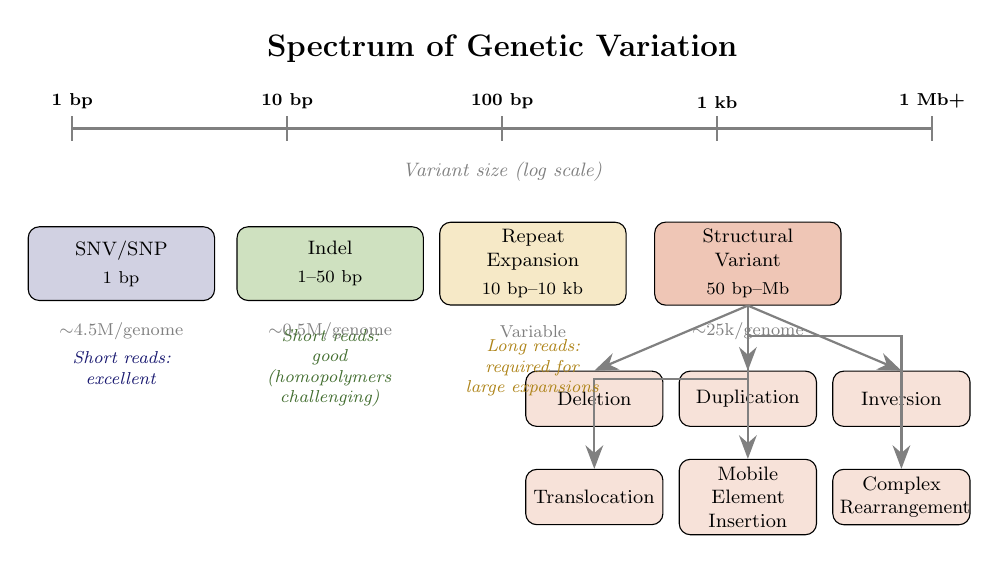
\begin{tikzpicture}[
  scale=0.78,
  transform shape,
  every node/.style={font=\small},
  varbox/.style={draw, rounded corners=4pt, minimum height=1.2cm, minimum width=3.0cm,
                 text width=2.8cm, align=center, font=\small},
  arrow/.style={-{Stealth[length=3mm]}, thick, gray},
  scalebar/.style={draw, thick, fill=gray!20, rounded corners=2pt, minimum height=0.5cm},
]

% Title
\node[font=\Large\bfseries] at (7, 10.5) {Spectrum of Genetic Variation};

% Scale bar at top
\draw[thick, gray] (0, 9.2) -- (14, 9.2);
\foreach \x/\lab in {0/1 bp, 3.5/10 bp, 7/100 bp, 10.5/1 kb, 14/1 Mb+} {
  \draw[thick, gray] (\x, 9.0) -- (\x, 9.4);
  \node[above, font=\footnotesize\bfseries] at (\x, 9.4) {\lab};
}
\node[font=\small\itshape, gray] at (7, 8.5) {Variant size (log scale)};

% SNV
\node[varbox, fill=MidnightBlue!20] (snv) at (0.8, 7) {SNV/SNP\\[2pt]\footnotesize 1 bp};

% Indel
\node[varbox, fill=OliveGreen!20] (indel) at (4.2, 7) {Indel\\[2pt]\footnotesize 1--50 bp};

% STR
\node[varbox, fill=Goldenrod!25] (str) at (7.5, 7) {Repeat\\Expansion\\[2pt]\footnotesize 10 bp--10 kb};

% SV
\node[varbox, fill=BrickRed!20] (sv) at (11, 7) {Structural\\Variant\\[2pt]\footnotesize 50 bp--Mb};

% Sub-types below SV
\node[varbox, fill=BrickRed!10, minimum width=2.2cm, text width=2.0cm, minimum height=0.9cm] (del) at (8.5, 4.8) {Deletion};
\node[varbox, fill=BrickRed!10, minimum width=2.2cm, text width=2.0cm, minimum height=0.9cm] (dup) at (11, 4.8) {Duplication};
\node[varbox, fill=BrickRed!10, minimum width=2.2cm, text width=2.0cm, minimum height=0.9cm] (inv) at (13.5, 4.8) {Inversion};
\node[varbox, fill=BrickRed!10, minimum width=2.2cm, text width=2.0cm, minimum height=0.9cm] (tra) at (8.5, 3.2) {Translocation};
\node[varbox, fill=BrickRed!10, minimum width=2.2cm, text width=2.0cm, minimum height=0.9cm] (mei) at (11, 3.2) {Mobile Element\\Insertion};
\node[varbox, fill=BrickRed!10, minimum width=2.2cm, text width=2.0cm, minimum height=0.9cm] (cpx) at (13.5, 3.2) {Complex\\Rearrangement};

% Arrows from SV to subtypes
\draw[arrow] (sv.south) -- (del.north);
\draw[arrow] (sv.south) -- (dup.north);
\draw[arrow] (sv.south) -- (inv.north);
\draw[arrow] (sv.south) -- ++(0, -1.2) -| (tra.north);
\draw[arrow] (sv.south) -- ++(0, -1.2) -| (mei.north);
\draw[arrow] (sv.south) -- ++(0, -0.5) -| (cpx.north);

% Detection method annotations
\node[font=\footnotesize\itshape, text=MidnightBlue, text width=2.5cm, align=center] at (0.8, 5.3) {Short reads:\\excellent};
\node[font=\footnotesize\itshape, text=OliveGreen!80!black, text width=2.5cm, align=center] at (4.2, 5.3) {Short reads:\\good\\(homopolymers\\challenging)};
\node[font=\footnotesize\itshape, text=Goldenrod!80!black, text width=2.5cm, align=center] at (7.5, 5.3) {Long reads:\\required for\\large expansions};

% Count annotations
\node[font=\footnotesize, text=gray] at (0.8, 5.9) {$\sim$4.5M/genome};
\node[font=\footnotesize, text=gray] at (4.2, 5.9) {$\sim$0.5M/genome};
\node[font=\footnotesize, text=gray] at (7.5, 5.9) {Variable};
\node[font=\footnotesize, text=gray] at (11, 5.9) {$\sim$25k/genome};

\end{tikzpicture}
\caption{The spectrum of genetic variation, from single nucleotide variants (SNVs) to complex structural rearrangements. Each variant class requires different detection strategies and tools. Sizes are shown on a logarithmic scale.}
\label{fig:variant_types}
\end{figure}

%% ============================================================
\section{Variant Calling Approaches}
\label{sec:variant_calling}
%% ============================================================

\subsection{Germline Variant Calling}

Germline variants are inherited and present in every cell of the body (or mosaic in a substantial fraction). They are called from a single sample, typically at 30$\times$ WGS or higher.

\subsubsection{GATK HaplotypeCaller}

The GATK HaplotypeCaller is the most widely used germline variant caller. Its approach:
\begin{enumerate}[nosep]
  \item \textbf{Active region detection}: Identifies regions with evidence of variation.
  \item \textbf{Local de novo assembly}: Builds a De Bruijn graph of reads in each active region to determine plausible haplotypes.
  \item \textbf{Pairwise read-haplotype alignment}: Aligns each read to each candidate haplotype using a pair-HMM algorithm.
  \item \textbf{Genotype likelihood calculation}: Computes likelihoods for each possible diploid genotype.
  \item \textbf{Output}: GVCF format (genomic VCF) with confidence scores for both variant and reference positions.
\end{enumerate}

For cohort analysis, the GATK Best Practices recommend a three-step process: (1) \textbf{HaplotypeCaller} per sample to produce GVCFs, (2) \textbf{GenomicsDBImport} to consolidate GVCFs, and (3) \textbf{GenotypeGVCFs} for joint genotyping across all samples.

\subsubsection{DeepVariant}

Google's DeepVariant reframes variant calling as an image classification problem:
\begin{enumerate}[nosep]
  \item Candidate variant sites are identified from pileup data.
  \item For each candidate, a multi-channel ``pileup image'' is constructed encoding read bases, quality scores, mapping quality, strand, and other features.
  \item A convolutional neural network (CNN) classifies each site as homozygous reference, heterozygous, or homozygous alternate.
  \item Specialised models exist for Illumina WGS, Illumina WES, PacBio HiFi, ONT, and hybrid data.
\end{enumerate}

DeepVariant consistently achieves the highest accuracy in the precisionFDA Truth Challenge and PrecisionFDA v2 benchmarks, particularly for indels.

\subsubsection{Joint Calling and GLnexus}

When analysing cohorts, joint calling improves sensitivity for rare variants and enables accurate genotyping at multi-allelic sites. \software{GLnexus} provides scalable joint genotyping from DeepVariant GVCFs:

\begin{itemize}[nosep]
  \item Handles hundreds of thousands of samples efficiently.
  \item Used by the All of Us program and UK Biobank for population-scale joint calling.
  \item Produces a project-level VCF with unified genotypes across all samples.
\end{itemize}

\subsection{Somatic Variant Calling}

Somatic variants arise in individual cells during the lifetime of an organism and are central to cancer genomics. They present unique challenges: they may be present at low variant allele frequencies (VAF), the tumor is heterogeneous (mixed clones), and there is no diploid genotype expectation.

\begin{keyconcept}[title={Tumor/Normal Paired Analysis}]
The gold standard for somatic variant calling uses a \textbf{matched tumor--normal pair}: the tumor sample and a normal sample (e.g., blood, adjacent normal tissue) from the same patient. Variants present in the tumor but absent from the normal are classified as somatic. This design filters out germline variants and sequencing artefacts that appear in both samples.
\end{keyconcept}

\subsubsection{Key Somatic Callers}

\begin{description}[style=nextline]
  \item[Mutect2 (GATK)] The most widely used somatic SNV/indel caller. Uses a Bayesian approach with a tumor-normal log-odds model. Supports tumor-only mode (with a panel of normals) and multi-sample calling. Includes \software{FilterMutectCalls} for artefact filtering using orientation bias models, contamination estimates, and a learned error model.
  \item[Strelka2] Developed by Illumina, Strelka2 is fast and accurate, using a mixture model for tumor--normal somatic variant calling. Also supports germline calling.
  \item[SomaticSniper] An earlier somatic caller based on a Bayesian genotype comparison between tumor and normal. Less commonly used now but conceptually important.
  \item[Consensus approach] Best practice in cancer genomics often involves running multiple callers and taking the intersection (high specificity) or union (high sensitivity) of their call sets, depending on the application.
\end{description}

\subsection{Structural Variant Calling}

SV calling remains more challenging than SNV/indel calling due to the diversity of SV types and the difficulty of resolving breakpoints in repetitive regions.

\begin{table}[htbp]
\centering
\caption{Structural variant callers for short-read and long-read data.}
\label{tab:sv_callers}
\begin{tabularx}{\textwidth}{@{}llXl@{}}
\toprule
\textbf{Tool} & \textbf{Data Type} & \textbf{SV Types} & \textbf{Approach} \\
\midrule
Manta & Short reads & DEL, DUP, INS, INV, BND & Discordant pairs + split reads + local assembly \\
DELLY & Short reads & DEL, DUP, INV, TRA, INS & Paired-end + split-read + read-depth \\
Smoove & Short reads & DEL, DUP, INV, BND & Wraps LUMPY with better filtering \\
Sniffles2 & Long reads & All SV types & Split-read alignment signatures \\
pbsv & PacBio & DEL, INS, DUP, INV, BND & CCS/HiFi signatures + local assembly \\
cuteSV & Long reads & DEL, INS, DUP, INV, BND & Clustering of SV signatures \\
SVIM & Long reads & All SV types & Multi-signature clustering \\
\bottomrule
\end{tabularx}
\end{table}

\subsection{Copy Number Variant Calling}

\begin{description}[style=nextline]
  \item[CNVnator] Read-depth--based CNV caller that divides the genome into bins and detects deviations from the expected diploid copy number using a mean-shift algorithm.
  \item[GATK gCNV (GermlineCNVCaller)] A cohort-based approach that models systematic coverage biases using a panel of normals and detects per-sample CNVs as deviations from the expected copy-number profile.
  \item[Spectre] Specifically designed for long-read CNV detection using coverage-based approaches.
  \item[ERDS, XHMM, CODEX2] Additional tools for WES-based CNV calling, which use the non-uniform exome capture data to infer copy number changes.
\end{description}

\subsection{Short Tandem Repeat Analysis}

\begin{description}[style=nextline]
  \item[ExpansionHunter] Developed by Illumina, uses paired-end and soft-clipped reads to estimate STR length, even when expansions exceed the read length. Supports a catalogue of $>$30 known pathogenic repeat loci.
  \item[STRique] Nanopore-specific STR quantification using raw signal data, enabling detection of very large expansions.
  \item[TRGT] PacBio's tandem repeat genotyping tool for HiFi data, providing allele-resolved repeat length and sequence composition.
  \item[STRling] Detects novel (uncatalogued) STR expansions from short-read data by identifying reads with excessive tandem repeat content.
\end{description}

\subsection{Haplotype Phasing}

Phasing determines which alleles at different variant sites reside on the same physical chromosome (haplotype).

\begin{description}[style=nextline]
  \item[WhatsHap] Read-backed phasing using long reads or linked reads. Formulates phasing as a weighted minimum error correction (wMEC) problem.
  \item[HiPhase] PacBio's phasing tool optimised for HiFi data, jointly phases SNVs, indels, and structural variants.
  \item[SHAPEIT5] Population-based statistical phasing using Hidden Markov Models. Leverages linkage disequilibrium patterns from large reference panels (e.g., TOPMed, 1000 Genomes) to phase common and rare variants.
\end{description}

%% ============================================================
\section{Variant Filtering and Quality Control}
\label{sec:variant_filter}
%% ============================================================

Raw variant calls contain many false positives due to sequencing errors, mapping artefacts, and systematic biases. Rigorous filtering is essential.

\subsection{GATK Variant Quality Score Recalibration (VQSR)}

VQSR is a machine learning--based approach that uses known, validated variant sites as ``truth'' training data to build a Gaussian mixture model in the space of variant quality annotations:

\begin{enumerate}[nosep]
  \item Training truth sets: HapMap3 sites, Omni 2.5M array sites, 1000 Genomes high-confidence SNPs, Mills gold-standard indels.
  \item Annotation features used: QualByDepth (QD), FisherStrand (FS), StrandOddsRatio (SOR), RMSMappingQuality (MQ), MappingQualityRankSumTest (MQRankSum), ReadPosRankSumTest (ReadPosRankSum), InbreedingCoeff.
  \item The model assigns each variant a VQSLOD score (log odds of being a true variant).
  \item Variants are filtered at a chosen sensitivity tranche (e.g., 99.5\% sensitivity retains 99.5\% of known truth set variants).
\end{enumerate}

\begin{warningbox}[title={When VQSR Fails}]
VQSR requires a minimum of $\sim$30 whole-genome samples (for SNPs) or $\sim$1 whole-genome sample (for indels) to build a reliable model. For small sample sizes, targeted panels, or non-human organisms without comprehensive truth sets, fall back to \textbf{hard filtering}.
\end{warningbox}

\subsection{Hard Filters}

When VQSR cannot be applied, GATK recommends the following hard filter thresholds for SNVs:

\begin{table}[htbp]
\centering
\caption{GATK recommended hard filters for SNVs and indels.}
\label{tab:hard_filters}
\begin{tabular}{@{}lll@{}}
\toprule
\textbf{Filter} & \textbf{SNV Threshold} & \textbf{Indel Threshold} \\
\midrule
QualByDepth (QD) & $<$ 2.0 & $<$ 2.0 \\
FisherStrand (FS) & $>$ 60.0 & $>$ 200.0 \\
StrandOddsRatio (SOR) & $>$ 3.0 & $>$ 10.0 \\
RMSMappingQuality (MQ) & $<$ 40.0 & --- \\
MQRankSum & $<$ $-$12.5 & --- \\
ReadPosRankSum & $<$ $-$8.0 & $<$ $-$20.0 \\
\bottomrule
\end{tabular}
\end{table}

%% ============================================================
\section{Statistical Foundations of Variant Calling}
\label{sec:variant_stats}
%% ============================================================

The variant calling algorithms described above rely on rigorous probabilistic models. This section formalises the key statistical machinery: the pair-HMM used for read--haplotype alignment, Bayesian genotyping, the VQSR Gaussian mixture model, and connections to population genetics.

\subsection{Pair-HMM for Read--Haplotype Alignment}
\label{subsec:variants:pairhmm}

At the core of \software{GATK HaplotypeCaller} is a \textbf{pair hidden Markov model (pair-HMM)} that computes the likelihood of observing a read given a candidate haplotype. The pair-HMM defines three emitting states:

\begin{description}[nosep]
  \item[Match / Mismatch (M)] Both the read and the haplotype advance by one position. The emission probability depends on whether the bases agree (match) or disagree (mismatch), weighted by the base quality score.
  \item[Insertion (I)] The read advances by one base, but the haplotype does not. Models insertions in the read relative to the haplotype.
  \item[Deletion (D)] The haplotype advances by one base, but the read does not. Models deletions in the read relative to the haplotype.
\end{description}

The transition probabilities between states are:
\begin{align}
\label{eq:variants:pairhmm_transitions}
P(M \to M) &= 1 - P(M \to I) - P(M \to D), \nonumber \\
P(M \to I) &= \delta_{\text{open}}, \qquad P(M \to D) = \delta_{\text{open}}, \nonumber \\
P(I \to I) &= \epsilon_{\text{extend}}, \qquad P(I \to M) = 1 - \epsilon_{\text{extend}}, \\
P(D \to D) &= \epsilon_{\text{extend}}, \qquad P(D \to M) = 1 - \epsilon_{\text{extend}}, \nonumber
\end{align}
where $\delta_{\text{open}}$ is the gap-opening probability and $\epsilon_{\text{extend}}$ is the gap-extension probability. In \software{GATK}, these probabilities are derived from the base insertion and deletion quality scores encoded in the BAM file (tags \texttt{BI} and \texttt{BD} after BQSR).

The likelihood of read $r$ given haplotype $h$ is computed via dynamic programming over the pair-HMM matrix in $O(|r| \times |h|)$ time:
\begin{equation}
\label{eq:variants:read_haplotype_likelihood}
P(r \mid h) = \sum_{j=1}^{|h|} \bigl[ M(|r|, j) + I(|r|, j) \bigr],
\end{equation}
where $M(i,j)$, $I(i,j)$, and $D(i,j)$ are the forward-algorithm probabilities of aligning the first $i$ bases of the read to the first $j$ bases of the haplotype, ending in state $M$, $I$, or $D$, respectively. This computation is the most computationally expensive step in \software{HaplotypeCaller} and is hardware-accelerated on Intel (AVX-512), GPU (NVIDIA), and FPGA platforms.

\begin{keyconcept}[title={Why Pair-HMM Instead of Standard Alignment?}]
Unlike Smith-Waterman or Needleman-Wunsch alignment, which return a single best alignment (and its score), the pair-HMM \emph{sums over all possible alignments}, yielding the total probability of the read given the haplotype. This marginalisation is critical for accurate genotyping because it avoids committing to a single alignment path when multiple near-optimal alignments exist, particularly in repetitive or low-complexity regions.
\end{keyconcept}

\subsection{Bayesian Genotyping}
\label{subsec:variants:bayesian_gt}

Given the pair-HMM likelihoods, genotype calling proceeds via Bayes' theorem. For a diploid site with candidate alleles $\{A_0, A_1, \ldots, A_m\}$, the possible genotypes are all unordered pairs $G = A_i / A_j$ ($i \leq j$). The posterior probability of genotype $G$ given observed data $D$ (the set of reads overlapping the site) is:
\begin{equation}
\label{eq:variants:genotype_posterior}
P(G \mid D) = \frac{P(D \mid G) \cdot P(G)}{\sum_{G'} P(D \mid G') \cdot P(G')},
\end{equation}
where $P(G)$ is the genotype prior (often derived from population allele frequencies or a flat prior) and $P(D \mid G)$ is the genotype likelihood.

For a diploid genotype $G = A_i / A_j$, the data likelihood assuming conditionally independent reads $\{r_1, \ldots, r_N\}$ is:
\begin{equation}
\label{eq:variants:genotype_likelihood}
P(D \mid G = A_i/A_j) = \prod_{n=1}^{N} \left[ \frac{1}{2}\, P(r_n \mid A_i) + \frac{1}{2}\, P(r_n \mid A_j) \right],
\end{equation}
where $P(r_n \mid A_i)$ is the pair-HMM probability of read $r_n$ given allele (haplotype) $A_i$.

\paragraph{VCF encoding of likelihoods.}
The VCF format encodes genotype likelihoods in two key fields:

\begin{description}[nosep]
  \item[PL (Phred-scaled Likelihood)] Defined as $\mathrm{PL}(G) = -10 \log_{10} P(D \mid G)$, normalised so that the most likely genotype has $\mathrm{PL} = 0$. Lower PL indicates a more likely genotype.
  \item[GQ (Genotype Quality)] The Phred-scaled confidence that the called genotype is correct, defined as the difference between the two lowest PL values:
    \begin{equation}
    \label{eq:variants:gq}
    \mathrm{GQ} = \mathrm{PL}_{\text{second-best}} - \mathrm{PL}_{\text{best}} = \mathrm{PL}_{\text{second-best}},
    \end{equation}
    since $\mathrm{PL}_{\text{best}} = 0$ by convention. A GQ of 30 means the probability of the called genotype being wrong is $\leq 10^{-3}$.
\end{description}

\begin{tipbox}[title={Minimum GQ Thresholds for Different Applications}]
Clinical germline analysis typically requires $\mathrm{GQ} \geq 20$ (99\% confidence). For population genetics studies where genotype accuracy is critical (e.g., identity-by-descent analysis, kinship estimation), a threshold of $\mathrm{GQ} \geq 30$ is common. For GWAS, imputation quality metrics ($R^2$ or INFO score) complement per-sample GQ.
\end{tipbox}

\subsection{VQSR: The Gaussian Mixture Model in Detail}
\label{subsec:variants:vqsr_detail}

Variant Quality Score Recalibration (introduced in \Cref{sec:variant_filter}) trains a \textbf{Gaussian mixture model (GMM)} to separate true variants from artefacts in a multi-dimensional annotation space. The procedure is as follows:

\begin{enumerate}[nosep]
  \item \textbf{Feature extraction}: Each variant site is described by a vector of quality annotations:
    \begin{itemize}[nosep]
      \item QualByDepth (QD): variant quality normalised by depth.
      \item MappingQuality (MQ): root-mean-square mapping quality of reads.
      \item FisherStrand (FS): Phred-scaled $p$-value of Fisher's exact test for strand bias.
      \item StrandOddsRatio (SOR): a more robust measure of strand bias using a symmetric odds ratio.
      \item MQRankSum: rank-sum test comparing mapping qualities of reference vs.\ alternate reads.
      \item ReadPosRankSum: rank-sum test comparing read positions of reference vs.\ alternate alleles (filters variants concentrated at read ends).
    \end{itemize}
  \item \textbf{GMM training}: The model fits $K$ Gaussian components to the annotation vectors of known true-positive sites (training resources: HapMap\,3, Omni\,2.5M, 1000 Genomes high-confidence sites for SNPs; Mills and 1000 Genomes gold-standard indels). The probability density for variant $\mathbf{x}$ under the GMM is:
    \begin{equation}
    \label{eq:variants:gmm}
    p(\mathbf{x}) = \sum_{k=1}^{K} \pi_k \, \mathcal{N}\!\left(\mathbf{x} \;\middle|\; \boldsymbol{\mu}_k, \boldsymbol{\Sigma}_k\right),
    \end{equation}
    where $\pi_k$ are mixing weights, $\boldsymbol{\mu}_k$ are component means, and $\boldsymbol{\Sigma}_k$ are covariance matrices. Parameters are estimated via Expectation-Maximisation (EM).
  \item \textbf{VQSLOD scoring}: Each variant receives a log-odds score comparing its probability under the ``true'' GMM vs.\ the ``false'' (background) distribution:
    \begin{equation}
    \label{eq:variants:vqslod}
    \mathrm{VQSLOD} = \log_{10} \frac{p(\mathbf{x} \mid \text{true})}{p(\mathbf{x} \mid \text{false})}.
    \end{equation}
  \item \textbf{Sensitivity tranches}: Rather than applying a fixed VQSLOD threshold, GATK defines tranches by the fraction of known truth-set variants retained. A tranche of 99.5\% means the VQSLOD cutoff is set to retain 99.5\% of HapMap\,3 sites. Lower tranches (e.g., 99.0\%) are more stringent; higher tranches (e.g., 99.9\%) retain more variants but include more false positives.
\end{enumerate}

\begin{warningbox}[title={VQSR Annotation Interactions}]
VQSR annotations are not independent. For example, variants in low-mappability regions tend to have low MQ, elevated FS, and extreme MQRankSum simultaneously. The multivariate Gaussian model captures these correlations through the full covariance matrix $\boldsymbol{\Sigma}_k$, which is why VQSR substantially outperforms univariate hard filters when sufficient training data are available.
\end{warningbox}

\subsection{Population Genetics Connections}
\label{subsec:variants:popgen}

Variant calling and quality control are deeply connected to population genetics theory. Several population-level statistics serve as powerful QC and analytical tools.

\subsubsection{Hardy-Weinberg Equilibrium as a QC Filter}

Under random mating, the genotype frequencies at a biallelic locus with allele frequencies $p$ (reference) and $q = 1 - p$ (alternate) are expected to follow Hardy-Weinberg Equilibrium (HWE):
\begin{equation}
\label{eq:variants:hwe}
f(AA) = p^2, \qquad f(Aa) = 2pq, \qquad f(aa) = q^2,
\end{equation}
where $p^2 + 2pq + q^2 = 1$. Departures from HWE---tested using a $\chi^2$ or exact test---can indicate:

\begin{itemize}[nosep]
  \item \textbf{Genotyping errors}: Excess homozygotes suggest allelic dropout; excess heterozygotes suggest systematic sequencing artefacts or paralogous mapping.
  \item \textbf{Population stratification}: Mixing individuals from different populations inflates heterozygosity (Wahlund effect).
  \item \textbf{Selection}: Strong selection against homozygotes (e.g., sickle-cell trait in malaria-endemic regions) creates genuine HWE departure.
\end{itemize}

\begin{protocolbox}[title={Applying HWE Filters in Practice}]
For QC of germline call sets:
\begin{enumerate}[nosep]
  \item Compute HWE $p$-values per site using \software{PLINK2} (\texttt{--hardy}) or \software{bcftools +fill-tags -- -t HWE}.
  \item Remove sites with extreme HWE deviation ($p < 10^{-6}$ is a common threshold for GWAS QC).
  \item Apply HWE filters \emph{within} each population stratum, not across the entire cohort, to avoid confounding with population structure.
\end{enumerate}
\end{protocolbox}

\subsubsection{Site Frequency Spectrum}

The \textbf{site frequency spectrum (SFS)}, also called the allele frequency spectrum, is the distribution of allele counts across polymorphic sites in a sample. For $n$ diploid individuals ($2n$ chromosomes), the SFS is a vector $\boldsymbol{\xi} = (\xi_1, \xi_2, \ldots, \xi_{2n-1})$, where $\xi_i$ is the number of sites at which the derived (or alternate) allele appears exactly $i$ times.

The SFS is a fundamental summary statistic because:
\begin{itemize}[nosep]
  \item Under the standard neutral model, the expected unfolded SFS follows $E[\xi_i] = \theta / i$, where $\theta = 4 N_e \mu$ is the population-scaled mutation rate. This predicts an excess of rare variants (singletons, doubletons).
  \item Departures from the neutral expectation reveal demographic history (bottlenecks, expansions) and selection (purifying selection depletes rare variants; balancing selection creates excess intermediate-frequency variants).
  \item The SFS is also a sensitive diagnostic for data quality: an excess of singletons can indicate sequencing errors rather than rare biological variants.
\end{itemize}

\subsubsection{$F_{\text{ST}}$ for Population Differentiation}

Fixation index $F_{\text{ST}}$ quantifies the degree of genetic differentiation between populations. Using Weir and Cockerham's estimator:
\begin{equation}
\label{eq:variants:fst}
F_{\text{ST}} = \frac{\sigma_a^2}{\sigma_a^2 + \sigma_b^2 + \sigma_w^2},
\end{equation}
where $\sigma_a^2$ is the variance component due to differences among populations, $\sigma_b^2$ is due to differences among individuals within populations, and $\sigma_w^2$ is within-individual variance. In the simpler Hudson estimator for two populations:
\begin{equation}
\label{eq:variants:fst_hudson}
F_{\text{ST}} = 1 - \frac{\bar{\pi}_w}{\pi_b},
\end{equation}
where $\bar{\pi}_w$ is the average within-population nucleotide diversity and $\pi_b$ is the between-population diversity.

\begin{description}[nosep]
  \item[$F_{\text{ST}} \approx 0$] No differentiation; allele frequencies are similar across populations.
  \item[$F_{\text{ST}} \approx 1$] Complete fixation of different alleles in different populations.
  \item[Genome-wide average in humans] $F_{\text{ST}} \approx 0.10$--$0.15$ between continental populations.
  \item[Outlier loci] Regions with $F_{\text{ST}}$ significantly above the genome-wide background are candidates for local adaptation (e.g., \gene{SLC24A5} for skin pigmentation, \gene{LCT} for lactase persistence).
\end{description}

Tools for computing $F_{\text{ST}}$ include \software{PLINK2}, \software{VCFtools}, \software{pixy} (which correctly handles missing data), and \software{scikit-allel}.

%% ============================================================
\section{Variant Annotation}
\label{sec:annotation}
%% ============================================================

After calling and filtering, variants must be annotated with functional, population, and clinical information to enable interpretation.

\subsection{Functional Annotation}

Functional annotation tools predict the consequence of each variant on genes, transcripts, and proteins:

\begin{description}[style=nextline]
  \item[VEP (Ensembl Variant Effect Predictor)] The most comprehensive annotation tool. Annotates variants with consequences (missense, frameshift, splice donor, etc.), affected transcripts, protein positions, and integrates plugins for pathogenicity scores, population frequencies, regulatory annotations, and more. Outputs in VCF, tab-delimited, or JSON format.
  \item[SnpEff] Fast Java-based annotator that classifies variants by impact (HIGH, MODERATE, LOW, MODIFIER). Useful for rapid annotation of large variant sets.
  \item[ANNOVAR] Perl-based tool supporting extensive database annotations. Widely used in clinical and research pipelines.
\end{description}

\subsection{Population Frequency Databases}

Population frequency is one of the most powerful filters for identifying pathogenic variants: truly deleterious variants are rare.

\begin{table}[htbp]
\centering
\caption{Major population frequency databases.}
\label{tab:pop_freq}
\begin{tabularx}{\textwidth}{@{}lXcc@{}}
\toprule
\textbf{Database} & \textbf{Description} & \textbf{Samples} & \textbf{Coverage} \\
\midrule
gnomAD v4 & Genome Aggregation Database. The largest publicly available collection of exome and genome variant frequencies. & $>$807,000 & WES + WGS \\
1000 Genomes Phase 3 & Foundational population genetics resource with 26 populations. & 2,504 & WGS (low-pass) \\
TOPMed & Trans-Omics for Precision Medicine. Deep WGS from diverse US populations. & $>$180,000 & WGS (30$\times$+) \\
UK Biobank & Exome sequencing of the UK Biobank cohort. & 500,000 & WES \\
ClinVar & Not a frequency database per se, but aggregates clinical significance classifications for variants. & --- & --- \\
\bottomrule
\end{tabularx}
\end{table}

\begin{tipbox}[title={Population Frequency Filtering}]
For rare Mendelian disease, filter out variants with a gnomAD population maximum allele frequency $>$0.01 (1\%) for dominant disorders or $>$0.03 (3\%) for recessive disorders. For ultra-rare conditions, use even stricter thresholds ($<$0.001). Always check population-specific frequencies, not just the global frequency, to avoid filtering out variants that are common in underrepresented populations.
\end{tipbox}

\subsection{Pathogenicity Prediction}

\begin{description}[style=nextline]
  \item[CADD (Combined Annotation Dependent Depletion)] Integrates 63+ annotations into a single deleteriousness score (Phred-scaled). CADD $\geq$20 indicates the top 1\% most deleterious variants; $\geq$30 the top 0.1\%.
  \item[REVEL (Rare Exome Variant Ensemble Learner)] An ensemble method combining 13 individual pathogenicity predictors (SIFT, PolyPhen-2, MutationTaster, etc.). Optimised for rare missense variants. Score range: 0 (benign) to 1 (pathogenic); threshold $\geq$0.5 is commonly used.
  \item[AlphaMissense] A deep learning model from DeepMind that predicts pathogenicity of all possible human missense variants using protein structure and evolutionary information from AlphaFold. Achieves state-of-the-art performance.
  \item[SpliceAI] Predicts the impact of variants on splicing by modelling the pre-mRNA sequence context using a deep residual neural network. Delta scores $\geq$0.5 indicate high splicing impact.
  \item[ClinVar] An NCBI database aggregating variant--disease associations and clinical significance classifications submitted by clinical laboratories and research groups.
  \item[OMIM] Online Mendelian Inheritance in Man. A curated catalogue of human genes and genetic disorders.
\end{description}

\subsection{Clinical Variant Classification: ACMG/AMP Guidelines}

The American College of Medical Genetics and Genomics (ACMG) and the Association for Molecular Pathology (AMP) jointly published a framework for classifying germline sequence variants into five tiers:

\begin{enumerate}[nosep]
  \item \textbf{Pathogenic}: Strong evidence that the variant causes disease.
  \item \textbf{Likely pathogenic}: Greater than 90\% probability of being disease-causing.
  \item \textbf{Variant of uncertain significance (VUS)}: Insufficient evidence to classify.
  \item \textbf{Likely benign}: Greater than 90\% probability of being benign.
  \item \textbf{Benign}: Strong evidence that the variant does not cause disease.
\end{enumerate}

Classification uses a set of criteria (evidence codes) such as:
\begin{itemize}[nosep]
  \item \textbf{PVS1}: Null variant (nonsense, frameshift, splice site $\pm$1,2) in a gene where loss-of-function is a known mechanism of disease.
  \item \textbf{PS1}: Same amino acid change as a previously established pathogenic variant.
  \item \textbf{PM2}: Absent from population databases (or at extremely low frequency).
  \item \textbf{PP3}: Computational evidence supports a deleterious effect (multiple in-silico tools agree).
  \item \textbf{BA1}: Allele frequency $>$5\% in gnomAD (standalone benign).
  \item \textbf{BS1}: Allele frequency greater than expected for the disorder.
\end{itemize}

Tools such as \software{InterVar} and \software{Franklin} automate ACMG classification, but expert clinical review remains essential for final interpretation.

%% ============================================================
\section{Cancer Genomics}
\label{sec:cancer_genomics}
%% ============================================================

Cancer genomics applies WGS, WES, and targeted panel sequencing to understand tumor biology and guide therapy.

\subsection{Tumor Mutational Burden (TMB)}

TMB is the total number of somatic non-synonymous mutations per megabase of coding sequence. It serves as a biomarker for response to immune checkpoint inhibitors (ICIs):

\begin{itemize}[nosep]
  \item \textbf{High TMB} ($\geq$10 mutations/Mb): Associated with better response to ICIs (pembrolizumab, nivolumab) across multiple cancer types. FDA-approved as a pan-cancer biomarker.
  \item TMB is typically measured from WES or large gene panels ($\geq$300 genes, $\geq$1\megabase{} target region).
  \item Cancers with highest TMB: melanoma (UV-induced), lung cancer (tobacco-induced), microsatellite-unstable cancers (MMR-deficient).
\end{itemize}

\subsection{Microsatellite Instability (MSI)}

MSI is caused by deficiency in DNA mismatch repair (MMR) genes (\gene{MLH1}, \gene{MSH2}, \gene{MSH6}, \gene{PMS2}). MSI-high (MSI-H) tumors accumulate thousands of somatic mutations, predominantly in microsatellite regions:

\begin{itemize}[nosep]
  \item Tools: \software{MSIsensor2}, \software{mSINGS}, \software{MANTIS}.
  \item MSI-H is an FDA-approved biomarker for pembrolizumab (Keytruda) across all solid tumors---the first tissue-agnostic cancer drug approval.
  \item Common in colorectal cancer ($\sim$15\%), endometrial cancer ($\sim$30\%), and gastric cancer.
\end{itemize}

\subsection{Mutational Signatures}

Mutational processes leave characteristic ``fingerprints'' in the genome---patterns of base substitutions, indels, and rearrangements. The COSMIC mutational signatures catalogue (v3.4) includes $>$100 signatures:

\begin{itemize}[nosep]
  \item \textbf{SBS1}: Clock-like, associated with 5mC deamination (C$>$T at CpG). Accumulates with age.
  \item \textbf{SBS4}: Tobacco smoking (C$>$A mutations).
  \item \textbf{SBS7a/b}: UV light (C$>$T at CC dinucleotides).
  \item \textbf{SBS6/15/20/26}: Mismatch repair deficiency.
  \item \textbf{SBS3}: Homologous recombination deficiency (BRCA1/2 deficiency)---clinically actionable for PARP inhibitor therapy.
  \item \textbf{SBS13/2}: APOBEC activity (C$>$T and C$>$G at TCA/TCT motifs).
  \item Tools: \software{SigProfiler}, \software{MutationalPatterns}, \software{deconstructSigs}.
\end{itemize}

\subsection{Tumor Heterogeneity and Clonal Evolution}

Tumors are not monolithic: they consist of genetically distinct subpopulations (clones) that evolve over time:

\begin{description}[style=nextline]
  \item[Clonal mutations] Present in all (or nearly all) cancer cells. These arose early in tumor development or represent the ancestral clone.
  \item[Subclonal mutations] Present in a fraction of cancer cells, representing branching evolution.
  \item[Variant allele frequency (VAF)] The fraction of reads supporting the alternate allele. In a diploid tumor, a clonal heterozygous mutation has VAF $\approx$ 0.5 $\times$ tumor purity. Subclonal mutations have lower VAF.
  \item[Tools] \software{PyClone-VI}, \software{SciClone}, \software{PhyloWGS}, \software{MOBSTER} reconstruct clonal architecture from VAF distributions.
\end{description}

\subsection{Liquid Biopsy and Cell-Free DNA (cfDNA)}

Liquid biopsy analyses cell-free DNA (cfDNA) circulating in blood, avoiding the need for invasive tissue biopsies:

\begin{itemize}[nosep]
  \item \textbf{Circulating tumor DNA (ctDNA)}: Tumor-derived cfDNA fragments, typically 0.01--10\% of total cfDNA in cancer patients.
  \item \textbf{Applications}: Non-invasive genotyping, monitoring treatment response, detecting minimal residual disease (MRD), early cancer detection (e.g., Galleri multi-cancer early detection test).
  \item \textbf{Technical requirements}: Ultra-deep sequencing (10,000--100,000$\times$ with UMIs), error-suppressed variant calling, tumour-informed or tumour-naive approaches.
  \item \textbf{Tools}: \software{ctDNAtools}, \software{ichorCNA} (estimates tumor fraction from cfDNA WGS), \software{MRDetect}.
  \item \textbf{Fragmentomics}: Analysis of cfDNA fragment size distributions, nucleosome positioning, and end motifs to infer tissue of origin and detect cancer.
\end{itemize}

%% ============================================================
\section{Pharmacogenomics}
\label{sec:pharmacogenomics}
%% ============================================================

Pharmacogenomics uses genetic information to predict individual drug response and guide medication selection and dosing.

\begin{keyconcept}[title={Key Pharmacogenes}]
\begin{description}[nosep]
  \item[\gene{CYP2D6}] Metabolises $\sim$25\% of all prescribed drugs. Highly polymorphic with $>$100 known alleles, gene deletions, and whole-gene duplications. Metaboliser phenotypes: poor, intermediate, normal (extensive), ultra-rapid.
  \item[\gene{CYP2C19}] Affects metabolism of clopidogrel (antiplatelet), proton pump inhibitors, and antidepressants. Loss-of-function alleles (CYP2C19*2, *3) reduce clopidogrel activation.
  \item[\gene{DPYD}] Dihydropyrimidine dehydrogenase---metabolises fluoropyrimidine chemotherapy (5-FU, capecitabine). DPD deficiency causes life-threatening toxicity.
  \item[\gene{TPMT}/\gene{NUDT15}] Affect metabolism of thiopurine drugs (azathioprine, 6-mercaptopurine). Deficiency causes severe myelosuppression.
  \item[\gene{VKORC1}] Affects sensitivity to warfarin (anticoagulant dosing).
  \item[\gene{HLA-B}] HLA-B*57:01 predicts abacavir hypersensitivity (HIV therapy); HLA-B*15:02 predicts carbamazepine-induced Stevens-Johnson syndrome.
\end{description}
Resources: PharmGKB database, CPIC (Clinical Pharmacogenetics Implementation Consortium) guidelines, DPWG (Dutch Pharmacogenetics Working Group) recommendations.
\end{keyconcept}

%% ============================================================
\section{Decision Flowchart: Variant Calling Pipeline Selection}
\label{sec:pipeline_decision}
%% ============================================================

\begin{figure}[htbp]
\centering
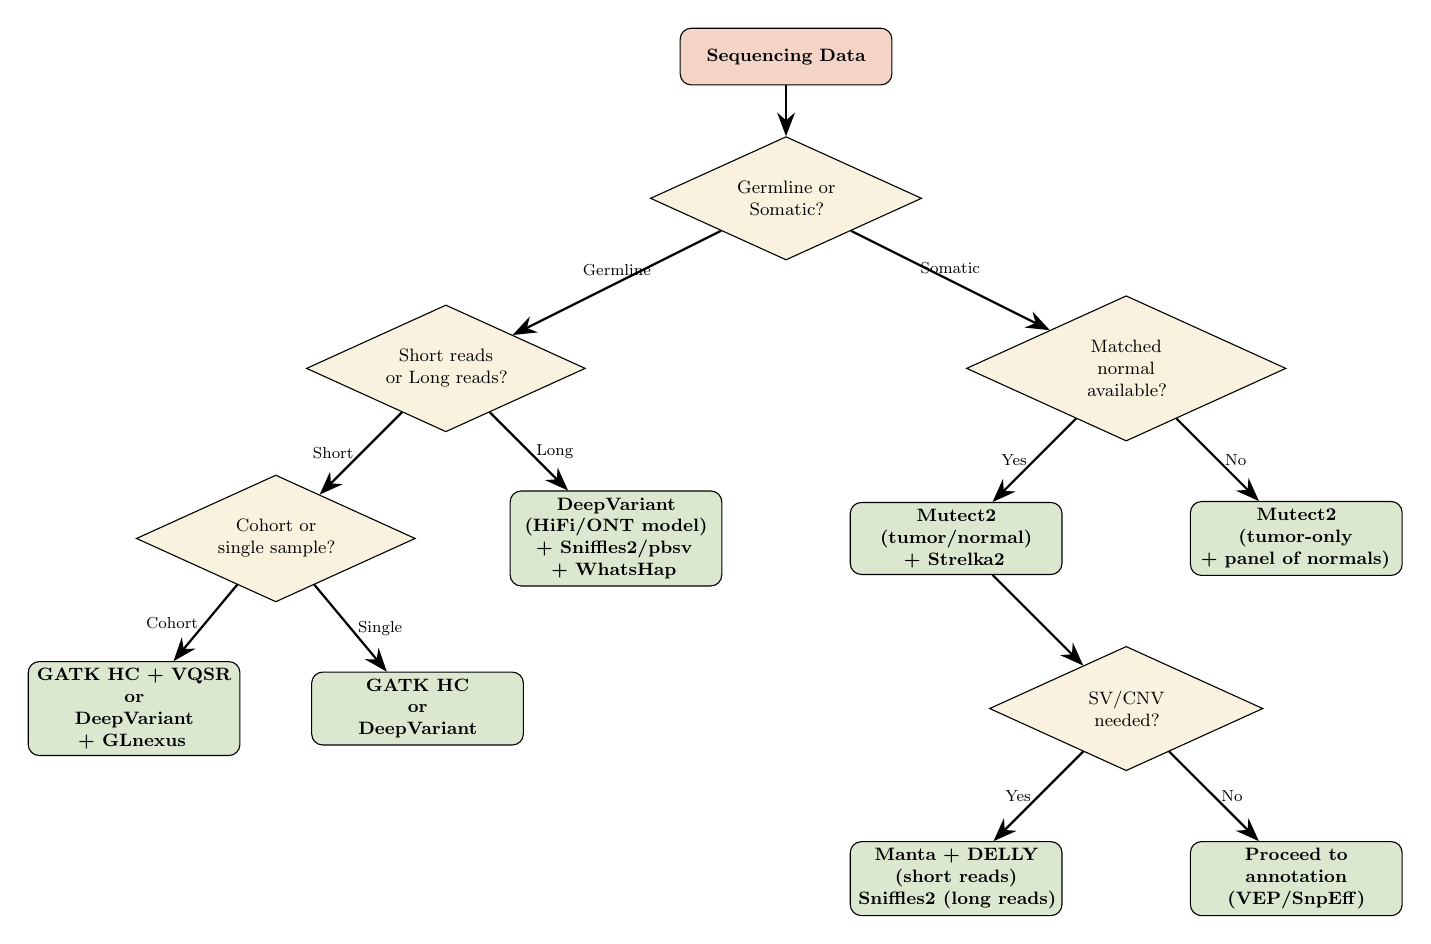
\begin{tikzpicture}[
  scale=0.72,
  transform shape,
  every node/.style={font=\small},
  decision/.style={diamond, draw, fill=Goldenrod!15, text width=3cm, align=center,
                   inner sep=2pt, aspect=2.2},
  process/.style={rectangle, draw, rounded corners=4pt, fill=MidnightBlue!12,
                  text width=3.5cm, align=center, minimum height=1cm},
  result/.style={rectangle, draw, rounded corners=4pt, fill=OliveGreen!15,
                 text width=3.5cm, align=center, minimum height=1cm, font=\small\bfseries},
  arrow/.style={-{Stealth[length=3mm]}, thick},
]

% Start
\node[process, fill=BrickRed!15, font=\small\bfseries] (start) at (0, 0) {Sequencing Data};

% Decision 1: Germline or Somatic?
\node[decision] (d1) at (0, -2.5) {Germline or\\Somatic?};
\draw[arrow] (start) -- (d1);

% Germline branch
\node[decision] (d2) at (-6, -5.5) {Short reads\\or Long reads?};
\draw[arrow] (d1) -- node[above, font=\footnotesize] {Germline} (d2);

% Germline short
\node[decision] (d3) at (-9, -8.5) {Cohort or\\single sample?};
\draw[arrow] (d2) -- node[left, font=\footnotesize] {Short} (d3);

\node[result] (r1) at (-11.5, -11.5) {GATK HC + VQSR\\or\\DeepVariant + GLnexus};
\draw[arrow] (d3) -- node[left, font=\footnotesize] {Cohort} (r1);

\node[result] (r2) at (-6.5, -11.5) {GATK HC\\or\\DeepVariant};
\draw[arrow] (d3) -- node[right, font=\footnotesize] {Single} (r2);

% Germline long
\node[result] (r3) at (-3, -8.5) {DeepVariant\\(HiFi/ONT model)\\+ Sniffles2/pbsv\\+ WhatsHap};
\draw[arrow] (d2) -- node[right, font=\footnotesize] {Long} (r3);

% Somatic branch
\node[decision] (d4) at (6, -5.5) {Matched\\normal\\available?};
\draw[arrow] (d1) -- node[above, font=\footnotesize] {Somatic} (d4);

\node[result] (r4) at (3, -8.5) {Mutect2\\(tumor/normal)\\+ Strelka2};
\draw[arrow] (d4) -- node[left, font=\footnotesize] {Yes} (r4);

\node[result] (r5) at (9, -8.5) {Mutect2\\(tumor-only\\+ panel of normals)};
\draw[arrow] (d4) -- node[right, font=\footnotesize] {No} (r5);

% SV branch from somatic
\node[decision] (d5) at (6, -11.5) {SV/CNV\\needed?};
\draw[arrow] (r4) -- (d5);

\node[result] (r6) at (3, -14.5) {Manta + DELLY\\(short reads)\\Sniffles2 (long reads)};
\draw[arrow] (d5) -- node[left, font=\footnotesize] {Yes} (r6);

\node[result] (r7) at (9, -14.5) {Proceed to\\annotation\\(VEP/SnpEff)};
\draw[arrow] (d5) -- node[right, font=\footnotesize] {No} (r7);

\end{tikzpicture}
\caption{Decision flowchart for selecting appropriate variant calling tools based on the experimental design, data type, and variant classes of interest.}
\label{fig:variant_pipeline_decision}
\end{figure}

%% ============================================================
\section{Practical Workflow: Variant Discovery Pipeline}
\label{sec:variant_pipeline}
%% ============================================================

The following Snakemake and Nextflow pipelines demonstrate a complete germline variant discovery workflow including calling, filtering, and annotation.

\subsection{Snakemake Variant Discovery Pipeline}

\begin{lstlisting}[language=Python, caption={Snakemake pipeline for germline variant calling, filtering, and annotation.}, label={lst:snakemake_variants}]
# Snakefile for Variant Discovery and Annotation
# Assumes aligned, deduplicated BAM files as input

configfile: "config.yaml"

SAMPLES = config["samples"]
REF = config["reference"]
KNOWN_SITES = config["known_sites"]
VEP_CACHE = config["vep_cache"]
VEP_SPECIES = "homo_sapiens"

rule all:
    input:
        expand("results/annotated/{sample}.annotated.vcf.gz",
               sample=SAMPLES),
        expand("results/sv/{sample}.manta.vcf.gz", sample=SAMPLES),
        expand("results/str/{sample}.eh.vcf.gz", sample=SAMPLES)

# --- GATK HaplotypeCaller (GVCF mode) ---
rule haplotypecaller:
    input:
        bam="data/bam/{sample}.dedup.bam",
        ref=REF
    output:
        gvcf="results/gvcf/{sample}.g.vcf.gz"
    threads: 4
    shell:
        """
        gatk HaplotypeCaller \
            -R {input.ref} -I {input.bam} \
            -O {output.gvcf} -ERC GVCF \
            --native-pair-hmm-threads {threads}
        """

# --- GenotypeGVCFs ---
rule genotype_gvcfs:
    input:
        gvcf="results/gvcf/{sample}.g.vcf.gz",
        ref=REF
    output:
        vcf="results/vcf/{sample}.raw.vcf.gz"
    shell:
        """
        gatk GenotypeGVCFs \
            -R {input.ref} -V {input.gvcf} \
            -O {output.vcf}
        """

# --- Hard Filtering (SNVs) ---
rule filter_snps:
    input:
        vcf="results/vcf/{sample}.raw.vcf.gz",
        ref=REF
    output:
        vcf="results/filtered/{sample}.snps.filtered.vcf.gz"
    shell:
        """
        gatk SelectVariants -R {input.ref} -V {input.vcf} \
            --select-type-to-include SNP \
            -O results/filtered/{wildcards.sample}.snps.raw.vcf.gz

        gatk VariantFiltration \
            -R {input.ref} \
            -V results/filtered/{wildcards.sample}.snps.raw.vcf.gz \
            --filter-expression "QD < 2.0" --filter-name "LowQD" \
            --filter-expression "FS > 60.0" --filter-name "HighFS" \
            --filter-expression "MQ < 40.0" --filter-name "LowMQ" \
            --filter-expression "SOR > 3.0" --filter-name "HighSOR" \
            --filter-expression "MQRankSum < -12.5" \
                --filter-name "LowMQRS" \
            --filter-expression "ReadPosRankSum < -8.0" \
                --filter-name "LowRPRS" \
            -O {output.vcf}
        """

# --- Hard Filtering (Indels) ---
rule filter_indels:
    input:
        vcf="results/vcf/{sample}.raw.vcf.gz",
        ref=REF
    output:
        vcf="results/filtered/{sample}.indels.filtered.vcf.gz"
    shell:
        """
        gatk SelectVariants -R {input.ref} -V {input.vcf} \
            --select-type-to-include INDEL \
            -O results/filtered/{wildcards.sample}.indels.raw.vcf.gz

        gatk VariantFiltration \
            -R {input.ref} \
            -V results/filtered/{wildcards.sample}.indels.raw.vcf.gz \
            --filter-expression "QD < 2.0" --filter-name "LowQD" \
            --filter-expression "FS > 200.0" --filter-name "HighFS" \
            --filter-expression "ReadPosRankSum < -20.0" \
                --filter-name "LowRPRS" \
            --filter-expression "SOR > 10.0" --filter-name "HighSOR" \
            -O {output.vcf}
        """

# --- Merge filtered SNPs and indels ---
rule merge_filtered:
    input:
        snps="results/filtered/{sample}.snps.filtered.vcf.gz",
        indels="results/filtered/{sample}.indels.filtered.vcf.gz"
    output:
        vcf="results/filtered/{sample}.merged.filtered.vcf.gz"
    shell:
        """
        gatk MergeVcfs \
            -I {input.snps} -I {input.indels} \
            -O {output.vcf}
        """

# --- VEP Annotation ---
rule vep_annotate:
    input:
        vcf="results/filtered/{sample}.merged.filtered.vcf.gz"
    output:
        vcf="results/annotated/{sample}.annotated.vcf.gz"
    params:
        cache=VEP_CACHE,
        species=VEP_SPECIES
    threads: 4
    shell:
        """
        vep --input_file {input.vcf} \
            --output_file {output.vcf} \
            --format vcf --vcf --compress_output bgzip \
            --cache --dir_cache {params.cache} \
            --species {params.species} --assembly GRCh38 \
            --everything --fork {threads} \
            --offline --force_overwrite
        """

# --- Structural Variant Calling (Manta) ---
rule manta_sv:
    input:
        bam="data/bam/{sample}.dedup.bam",
        ref=REF
    output:
        vcf="results/sv/{sample}.manta.vcf.gz"
    threads: 8
    shell:
        """
        configManta.py \
            --bam {input.bam} \
            --referenceFasta {input.ref} \
            --runDir results/sv/{wildcards.sample}_manta

        results/sv/{wildcards.sample}_manta/runWorkflow.py \
            -j {threads}

        cp results/sv/{wildcards.sample}_manta/results/variants/\
diploidSV.vcf.gz {output.vcf}
        """

# --- STR Expansion Analysis ---
rule expansion_hunter:
    input:
        bam="data/bam/{sample}.dedup.bam",
        ref=REF,
        catalog="resources/variant_catalog.json"
    output:
        vcf="results/str/{sample}.eh.vcf.gz"
    shell:
        """
        ExpansionHunter \
            --reads {input.bam} \
            --reference {input.ref} \
            --variant-catalog {input.catalog} \
            --output-prefix results/str/{wildcards.sample}.eh

        bgzip -c results/str/{wildcards.sample}.eh.vcf \
            > {output.vcf}
        tabix -p vcf {output.vcf}
        """
\end{lstlisting}

\subsection{Nextflow Variant Discovery Pipeline}

\begin{lstlisting}[language=Java, caption={Nextflow DSL2 pipeline for variant calling, filtering, and annotation.}, label={lst:nextflow_variants}]
#!/usr/bin/env nextflow
nextflow.enable.dsl=2

// Variant Discovery and Annotation Pipeline

params.bams      = "data/bam/*.dedup.bam"
params.ref       = "reference/hg38.fa"
params.vep_cache = "resources/vep_cache"
params.str_cat   = "resources/variant_catalog.json"
params.outdir    = "results"

process HAPLOTYPECALLER {
    tag "$sample_id"
    publishDir "${params.outdir}/gvcf", mode: 'copy'
    cpus 4

    input:
    tuple val(sample_id), path(bam), path(bai)
    path ref
    path ref_fai
    path ref_dict

    output:
    tuple val(sample_id), path("${sample_id}.g.vcf.gz"),
          path("${sample_id}.g.vcf.gz.tbi"),
          emit: gvcf

    script:
    """
    gatk HaplotypeCaller \
        -R ${ref} -I ${bam} \
        -O ${sample_id}.g.vcf.gz -ERC GVCF \
        --native-pair-hmm-threads ${task.cpus}
    """
}

process GENOTYPE_GVCFS {
    tag "$sample_id"
    publishDir "${params.outdir}/vcf", mode: 'copy'

    input:
    tuple val(sample_id), path(gvcf), path(gvcf_tbi)
    path ref
    path ref_fai
    path ref_dict

    output:
    tuple val(sample_id), path("${sample_id}.raw.vcf.gz"),
          path("${sample_id}.raw.vcf.gz.tbi"),
          emit: raw_vcf

    script:
    """
    gatk GenotypeGVCFs \
        -R ${ref} -V ${gvcf} \
        -O ${sample_id}.raw.vcf.gz
    """
}

process HARD_FILTER {
    tag "$sample_id"
    publishDir "${params.outdir}/filtered", mode: 'copy'

    input:
    tuple val(sample_id), path(vcf), path(vcf_tbi)
    path ref
    path ref_fai
    path ref_dict

    output:
    tuple val(sample_id),
          path("${sample_id}.filtered.vcf.gz"),
          path("${sample_id}.filtered.vcf.gz.tbi"),
          emit: filtered_vcf

    script:
    """
    # Filter SNPs
    gatk SelectVariants -R ${ref} -V ${vcf} \
        --select-type-to-include SNP \
        -O ${sample_id}.snps.vcf.gz
    gatk VariantFiltration -R ${ref} \
        -V ${sample_id}.snps.vcf.gz \
        --filter-expression "QD < 2.0" --filter-name "LowQD" \
        --filter-expression "FS > 60.0" --filter-name "HighFS" \
        --filter-expression "MQ < 40.0" --filter-name "LowMQ" \
        --filter-expression "SOR > 3.0" --filter-name "HighSOR" \
        -O ${sample_id}.snps.filt.vcf.gz

    # Filter Indels
    gatk SelectVariants -R ${ref} -V ${vcf} \
        --select-type-to-include INDEL \
        -O ${sample_id}.indels.vcf.gz
    gatk VariantFiltration -R ${ref} \
        -V ${sample_id}.indels.vcf.gz \
        --filter-expression "QD < 2.0" --filter-name "LowQD" \
        --filter-expression "FS > 200.0" --filter-name "HighFS" \
        --filter-expression "SOR > 10.0" --filter-name "HighSOR" \
        -O ${sample_id}.indels.filt.vcf.gz

    # Merge
    gatk MergeVcfs \
        -I ${sample_id}.snps.filt.vcf.gz \
        -I ${sample_id}.indels.filt.vcf.gz \
        -O ${sample_id}.filtered.vcf.gz
    """
}

process VEP_ANNOTATE {
    tag "$sample_id"
    publishDir "${params.outdir}/annotated", mode: 'copy'
    cpus 4

    input:
    tuple val(sample_id), path(vcf), path(vcf_tbi)
    path vep_cache

    output:
    tuple val(sample_id),
          path("${sample_id}.annotated.vcf.gz"),
          emit: annotated_vcf

    script:
    """
    vep --input_file ${vcf} \
        --output_file ${sample_id}.annotated.vcf.gz \
        --format vcf --vcf --compress_output bgzip \
        --cache --dir_cache ${vep_cache} \
        --species homo_sapiens --assembly GRCh38 \
        --everything --fork ${task.cpus} \
        --offline --force_overwrite
    """
}

process MANTA_SV {
    tag "$sample_id"
    publishDir "${params.outdir}/sv", mode: 'copy'
    cpus 8

    input:
    tuple val(sample_id), path(bam), path(bai)
    path ref
    path ref_fai

    output:
    tuple val(sample_id),
          path("${sample_id}.manta.sv.vcf.gz"),
          emit: sv_vcf

    script:
    """
    configManta.py \
        --bam ${bam} \
        --referenceFasta ${ref} \
        --runDir manta_run
    manta_run/runWorkflow.py -j ${task.cpus}
    cp manta_run/results/variants/diploidSV.vcf.gz \
        ${sample_id}.manta.sv.vcf.gz
    """
}

process EXPANSION_HUNTER {
    tag "$sample_id"
    publishDir "${params.outdir}/str", mode: 'copy'

    input:
    tuple val(sample_id), path(bam), path(bai)
    path ref
    path str_catalog

    output:
    tuple val(sample_id),
          path("${sample_id}.eh.vcf.gz"),
          emit: str_vcf

    script:
    """
    ExpansionHunter \
        --reads ${bam} --reference ${ref} \
        --variant-catalog ${str_catalog} \
        --output-prefix ${sample_id}.eh
    bgzip -c ${sample_id}.eh.vcf > ${sample_id}.eh.vcf.gz
    tabix -p vcf ${sample_id}.eh.vcf.gz
    """
}

// ---- Workflow ----
workflow {
    // Input channels
    bam_ch = Channel
        .fromFilePairs(params.bams, size: 1) { file ->
            file.name.replaceAll('.dedup.bam', '')
        }
        .map { id, files -> tuple(id, files[0],
                file("${files[0]}.bai")) }

    ref       = file(params.ref)
    ref_fai   = file("${params.ref}.fai")
    ref_dict  = file(params.ref.replaceAll('.fa$', '.dict'))
    vep_cache = file(params.vep_cache)
    str_cat   = file(params.str_cat)

    // Variant calling
    HAPLOTYPECALLER(bam_ch, ref, ref_fai, ref_dict)
    GENOTYPE_GVCFS(HAPLOTYPECALLER.out.gvcf,
                   ref, ref_fai, ref_dict)

    // Filtering and annotation
    HARD_FILTER(GENOTYPE_GVCFS.out.raw_vcf,
                ref, ref_fai, ref_dict)
    VEP_ANNOTATE(HARD_FILTER.out.filtered_vcf, vep_cache)

    // SV calling and STR analysis (parallel)
    MANTA_SV(bam_ch, ref, ref_fai)
    EXPANSION_HUNTER(bam_ch, ref, str_cat)
}
\end{lstlisting}

%% ============================================================
\section{Variant Calling Tool Comparison}
\label{sec:tool_comparison}
%% ============================================================

\begin{table}[htbp]
\centering
\caption{Comparison of variant calling tools for different variant classes and use cases.}
\label{tab:variant_tool_comparison}
\small
\begin{tabularx}{\textwidth}{@{}l*{4}{>{\raggedright\arraybackslash}X}@{}}
\toprule
\textbf{Variant Class} & \textbf{Tool} & \textbf{Approach} & \textbf{Data Type} & \textbf{Key Strengths} \\
\midrule
\multirow{2}{*}{Germline SNV/indel} & GATK HC & Local assembly + pair-HMM & Short reads & Gold standard, cohort support \\
 & DeepVariant & CNN image classification & Short/long reads & Highest accuracy, multi-platform \\
\addlinespace
\multirow{2}{*}{Somatic SNV/indel} & Mutect2 & Bayesian somatic model & Short reads & T/N and tumor-only modes \\
 & Strelka2 & Mixture model & Short reads & Fast, accurate \\
\addlinespace
\multirow{3}{*}{Structural variants} & Manta & Assembly + PE/SR & Short reads & Fast, comprehensive \\
 & Sniffles2 & Split-read signatures & Long reads & Gold standard for LR SVs \\
 & DELLY & PE + SR + RD & Short reads & Multi-algorithm, genotyping \\
\addlinespace
\multirow{2}{*}{CNVs} & GATK gCNV & Cohort denoising & WES/WGS & Handles capture bias \\
 & CNVnator & Read depth binning & WGS & Simple, effective \\
\addlinespace
\multirow{2}{*}{STR expansions} & ExpansionHunter & Spanning/flanking reads & Short reads & Known locus catalogue \\
 & TRGT & HiFi repeat analysis & PacBio HiFi & Allele-resolved, accurate \\
\addlinespace
\multirow{2}{*}{Phasing} & WhatsHap & Read-backed wMEC & Long reads & Physical phasing \\
 & SHAPEIT5 & Statistical HMM & Any (population) & Population-scale \\
\bottomrule
\end{tabularx}
\end{table}

%% ============================================================
\section{Summary}
\label{sec:ch08_summary}
%% ============================================================

\begin{keyconcept}[title={Chapter Summary}]
\begin{itemize}[nosep]
  \item Genetic variants range from single nucleotide changes (SNVs) to chromosome-scale structural rearrangements, each requiring specialised detection methods.
  \item \textbf{Germline variant calling} (GATK HaplotypeCaller, DeepVariant) identifies inherited variants; \textbf{somatic calling} (Mutect2, Strelka2) identifies cancer-specific mutations using tumor--normal pairs.
  \item \textbf{Structural variants and repeat expansions} require long reads or specialised short-read algorithms (Manta, ExpansionHunter) for reliable detection.
  \item Variant \textbf{filtering} (VQSR or hard filters) is essential to remove artefacts, and \textbf{annotation} (VEP, gnomAD, CADD, ClinVar) is required for biological and clinical interpretation.
  \item The \textbf{ACMG/AMP 5-tier classification} system provides a standardised framework for clinical variant interpretation.
  \item Cancer genomics applications include \textbf{TMB}, \textbf{MSI}, \textbf{mutational signatures}, \textbf{clonal analysis}, and \textbf{liquid biopsy} for non-invasive monitoring.
  \item \textbf{Pharmacogenomics} translates genetic variants in drug-metabolising enzymes and drug targets into actionable prescribing guidance.
\end{itemize}
\end{keyconcept}

\chapter{Metagenomics and Microbiome Sequencing}
\label{ch:metagenomics}

The world teems with microbial life. A single gram of soil contains billions of bacteria from thousands of species; the human gut harbours a community of trillions of microorganisms whose collective genome dwarfs our own. Traditionally, studying these communities required culturing individual organisms in the laboratory---a process that captures only an estimated 1\% of environmental microbial diversity. Metagenomics bypasses this ``great plate count anomaly'' by sequencing DNA directly from environmental or clinical samples, revealing the full genetic repertoire of entire microbial communities. This chapter covers both amplicon-based and shotgun metagenomic approaches, along with the computational tools needed to extract biological insight from complex community data.

%% ============================================================
\section{What Is Metagenomics?}
\label{sec:metagenomics_intro}
%% ============================================================

Metagenomics is the study of genetic material recovered directly from environmental or host-associated samples. Unlike single-organism genomics, metagenomics captures DNA from all organisms present in a sample---bacteria, archaea, fungi, protists, viruses, and host cells---in a single experiment.

\begin{keyconcept}[title={Metagenomics vs.\ Metatranscriptomics vs.\ Metaproteomics}]
\begin{description}[nosep]
  \item[Metagenomics] Sequences total DNA. Reveals which organisms are present and their \emph{functional potential} (all genes encoded). Cannot distinguish active from dormant organisms.
  \item[Metatranscriptomics] Sequences total RNA (after rRNA depletion). Reveals which genes are \emph{actively expressed} and by which organisms.
  \item[Metaproteomics] Identifies proteins via mass spectrometry. Reveals which proteins are actually produced and in what abundance.
\end{description}
Each layer provides complementary information. This chapter focuses on DNA-level metagenomics with a brief treatment of metatranscriptomics.
\end{keyconcept}

\subsection{The Microbiome: What It Is and Why It Matters}

The term \textbf{microbiome} refers to the community of microorganisms (and their collective genomes) inhabiting a defined environment. Key microbiome niches include:

\begin{description}[style=nextline]
  \item[Human gut microbiome] The most intensively studied microbiome. Contains $\sim$10$^{13}$ bacterial cells and $\sim$1,000 species per individual. Influences digestion, immune system development, pathogen resistance, drug metabolism, and even neurological function via the gut--brain axis. Dysbiosis (microbial imbalance) is implicated in inflammatory bowel disease, obesity, type 2 diabetes, colorectal cancer, and depression.
  \item[Human skin microbiome] Varies dramatically by body site (moist vs.\ dry vs.\ sebaceous). Dominated by \species{Cutibacterium}, \species{Staphylococcus}, and \species{Corynebacterium}. Relevant to atopic dermatitis, acne, wound healing.
  \item[Human oral microbiome] $>$700 species. Key to dental caries, periodontal disease, and increasingly linked to systemic diseases (cardiovascular disease, Alzheimer's disease).
  \item[Soil microbiome] The most diverse microbial ecosystem on Earth. Critical for nutrient cycling (nitrogen fixation, carbon decomposition), plant health, and agricultural productivity.
  \item[Marine microbiome] Oceanic microbes drive global biogeochemical cycles, producing $\sim$50\% of Earth's oxygen via photosynthesis.
  \item[Built environment] Indoor microbiomes (hospitals, homes, spacecraft) affect human health and building integrity.
\end{description}

%% ============================================================
\section{16S/18S/ITS Amplicon Sequencing}
\label{sec:amplicon}
%% ============================================================

Amplicon sequencing targets a specific phylogenetic marker gene to identify and quantify organisms in a sample. It is the most cost-effective approach for profiling microbial community composition.

\subsection{The 16S rRNA Gene}

The 16S ribosomal RNA gene ($\sim$1,540\basepair{}) is the most widely used phylogenetic marker for bacteria and archaea. It is ideal because:

\begin{itemize}[nosep]
  \item It is present in all bacteria and archaea (universal).
  \item It contains both highly \textbf{conserved regions} (for universal primer design) and \textbf{variable regions} (V1--V9) that differ between taxa, enabling taxonomic classification.
  \item Extensive reference databases exist (SILVA, Greengenes2) with $>$10 million curated sequences.
\end{itemize}

\subsubsection{Variable Region Selection}

The choice of which variable region(s) to amplify affects taxonomic resolution and which taxa are detected:

\begin{table}[htbp]
\centering
\caption{Commonly targeted 16S rRNA variable regions.}
\label{tab:16s_regions}
\begin{tabularx}{\textwidth}{@{}lcXl@{}}
\toprule
\textbf{Region} & \textbf{Length} & \textbf{Notes} & \textbf{Common Primers} \\
\midrule
V1--V2 & $\sim$300\basepair{} & Good for \species{Staphylococcus} differentiation; poor for some Enterobacteriaceae & 27F / 338R \\
V3--V4 & $\sim$460\basepair{} & \textbf{Most widely used}. Good overall taxonomic resolution. Standard for Illumina MiSeq 2$\times$300\basepair{} & 341F / 805R \\
V4 & $\sim$250\basepair{} & Used in the Earth Microbiome Project. Compatible with 2$\times$150\basepair{} & 515F / 806R \\
V4--V5 & $\sim$400\basepair{} & Better discrimination of archaea & 515F / 926R \\
Full-length & $\sim$1,500\basepair{} & Highest resolution. Requires long-read sequencing (PacBio, ONT) & 27F / 1492R \\
\bottomrule
\end{tabularx}
\end{table}

\begin{warningbox}[title={Primer Bias}]
No primer pair amplifies all taxa equally. Every primer set has biases---some taxa are underrepresented or missed entirely. The commonly used 515F/806R primers, for instance, have known biases against certain \species{Crenarchaeota} and \species{SAR11} marine bacteria. Always report which primer pair was used, and be cautious about comparing studies that used different primers.
\end{warningbox}

\subsection{Other Marker Genes}

\begin{description}[style=nextline]
  \item[18S rRNA] The eukaryotic equivalent of 16S rRNA. Used for profiling eukaryotic microbes (protists, micro-algae, nematodes, fungi). Variable regions (V4 and V9 are common) provide taxonomic resolution.
  \item[ITS (Internal Transcribed Spacer)] The ITS1 and ITS2 regions flanking the 5.8S rRNA gene are the standard barcodes for fungi. ITS evolves faster than 18S, providing species-level resolution for many fungal taxa. Reference database: UNITE.
\end{description}

\subsection{ASVs vs.\ OTUs}

A critical methodological decision in amplicon analysis is how to define taxonomic units:

\begin{description}[style=nextline]
  \item[OTU (Operational Taxonomic Unit)] Sequences are clustered at a similarity threshold (traditionally 97\% identity). Each cluster represents an ``OTU.'' This approach is tolerant of sequencing errors but sacrifices resolution and can merge distinct species. Tools: \software{USEARCH} (UPARSE algorithm), \software{VSEARCH}, \software{mothur}.
  \item[ASV (Amplicon Sequence Variant)] Error-correction algorithms model the sequencing error process and resolve sequences to single-nucleotide resolution. ASVs are exact biological sequences (after denoising), enabling comparison across studies, strain-level discrimination, and greater ecological precision. This is now the recommended approach. Tools: \software{DADA2}, \software{Deblur}.
\end{description}

\begin{keyconcept}[title={Why ASVs Have Replaced OTUs}]
ASVs offer multiple advantages over OTUs:
\begin{itemize}[nosep]
  \item \textbf{Reproducibility}: ASVs are exact sequences, so results from different studies are directly comparable. OTUs depend on the clustering algorithm and reference database.
  \item \textbf{Resolution}: ASVs can distinguish sequences differing by a single nucleotide, enabling strain-level discrimination.
  \item \textbf{Reusability}: ASV tables can be merged across experiments; OTU tables cannot (different OTU IDs in different studies).
  \item \textbf{No arbitrary threshold}: OTU clustering at 97\% is a historical convention with no biological basis for most taxa.
\end{itemize}
\end{keyconcept}

\subsection{Amplicon Analysis Tools}

\begin{description}[style=nextline]
  \item[QIIME 2] The most comprehensive amplicon analysis platform. Provides a plugin-based architecture for denoising (DADA2, Deblur), taxonomy assignment, diversity analysis, statistical testing, and visualisation. Produces interactive visualisations. The community standard for reproducible microbiome research.
  \item[DADA2] An R package for high-resolution amplicon denoising. The core algorithm models Illumina error profiles to distinguish true biological sequences from sequencing errors. Can also process PacBio and ONT full-length 16S data.
  \item[mothur] A long-established, comprehensive tool for amplicon analysis, particularly popular in the ecological microbiology community. Implements OTU-based workflows.
  \item[USEARCH / VSEARCH] Fast sequence analysis tools. VSEARCH is the open-source alternative to USEARCH.
\end{description}

\subsection{Taxonomic Classification Databases}

\begin{table}[htbp]
\centering
\caption{Major taxonomic reference databases for amplicon sequencing.}
\label{tab:tax_databases}
\begin{tabularx}{\textwidth}{@{}llXl@{}}
\toprule
\textbf{Database} & \textbf{Target} & \textbf{Description} & \textbf{Taxonomy} \\
\midrule
SILVA & 16S/18S/23S/28S & Comprehensive, curated rRNA database. $>$10M sequences. Updated regularly. & SILVA taxonomy \\
Greengenes2 & 16S & Rebuilt using whole-genome phylogenetics (\software{WoL2} backbone). Provides more accurate taxonomy than the original Greengenes. & GTDB-aligned \\
UNITE & ITS & The standard for fungal ITS taxonomy. Species hypothesis concept for dynamic species delimitation. & UNITE taxonomy \\
RDP & 16S/28S & Ribosomal Database Project. Provides a naive Bayesian classifier widely used for taxonomic assignment. & RDP taxonomy \\
GTDB & Whole genomes & Genome Taxonomy Database. Defines taxonomy using genome phylogeny (average nucleotide identity, RED). Not an rRNA database, but provides the taxonomic backbone increasingly used by 16S databases. & GTDB taxonomy \\
\bottomrule
\end{tabularx}
\end{table}

%% ============================================================
\section{Shotgun Metagenomics}
\label{sec:shotgun}
%% ============================================================

Shotgun metagenomics sequences all DNA in a sample (after fragmenting and library preparation), without any targeted amplification. This provides a far richer view of the community than amplicon sequencing.

\subsection{Advantages over Amplicon Sequencing}

\begin{itemize}[nosep]
  \item \textbf{All domains of life}: Detects bacteria, archaea, fungi, protists, and viruses simultaneously, without primer bias.
  \item \textbf{Functional potential}: Reveals the full gene content of the community---metabolic pathways, virulence factors, antibiotic resistance genes, secondary metabolite biosynthesis clusters.
  \item \textbf{Strain-level resolution}: Sufficient sequence diversity to distinguish closely related strains of the same species.
  \item \textbf{Metagenome-assembled genomes (MAGs)}: Shotgun data can be assembled and binned to reconstruct near-complete genomes of uncultured organisms.
  \item \textbf{No amplification bias}: Coverage reflects actual DNA abundance (modulo extraction bias and differential lysis).
\end{itemize}

\subsection{Library Preparation Considerations}

\begin{itemize}[nosep]
  \item \textbf{DNA extraction}: Different extraction protocols lyse different organisms with varying efficiency. Bead-beating protocols improve recovery of Gram-positive bacteria and fungi but may shear DNA. Standardised protocols (e.g., the International Human Microbiome Standards, IHMS) are essential for reproducibility.
  \item \textbf{Host DNA depletion}: For host-associated samples (e.g., human gut biopsies, respiratory samples), host DNA can dominate the library. Depletion strategies include differential lysis (saponin for human cells + DNase treatment), CpG methylation-based depletion (\software{NEBNext Microbiome DNA Enrichment Kit}), and propidium monoazide (PMA) treatment to remove extracellular/dead cell DNA.
  \item \textbf{Sequencing depth}: Sufficient depth depends on community complexity. Simple communities (e.g., fermented foods, $<$50 species) may require only 1--5 million read pairs. Complex communities (e.g., soil, $>$10,000 species) may require 50--200 million read pairs for adequate functional profiling and MAG recovery.
\end{itemize}

\begin{tipbox}[title={Estimating Required Sequencing Depth}]
A useful rule of thumb for human gut metagenomics:
\begin{itemize}[nosep]
  \item \textbf{5--10M read pairs}: Adequate for taxonomic profiling of dominant species.
  \item \textbf{20--50M read pairs}: Sufficient for functional profiling and detection of less abundant taxa.
  \item \textbf{$>$100M read pairs}: Required for strain-level analysis, rare species detection, and high-quality MAG recovery.
\end{itemize}
For soil or other hyper-diverse environments, even 200M read pairs may only scratch the surface. Consider long-read metagenomics for improved assembly of complex communities.
\end{tipbox}

\subsection{Taxonomic Profiling}

Taxonomic profiling assigns each read (or contig) to a taxonomic lineage.

\begin{description}[style=nextline]
  \item[Kraken2 / Bracken] \software{Kraken2} uses exact k-mer matching against a prebuilt database to classify reads at very high speed ($>$1 million reads/second). Each read is assigned to the lowest common ancestor (LCA) of all species sharing its k-mers. \software{Bracken} (Bayesian Reestimation of Abundance with KrakEN) then redistributes reads from higher taxonomic levels to species level using a Bayesian model of read-length--specific probabilities. Database: standard Kraken2 database includes RefSeq bacteria, archaea, viruses, and human; custom databases can include fungi, protozoa, and UniVec.
  \item[MetaPhlAn 4] Uses a database of clade-specific marker genes ($\sim$5.1M markers from $\sim$26,000 species) to estimate relative abundance. Highly specific but may miss novel species absent from the marker database. Reports relative abundance (not absolute counts).
  \item[mOTUs3] Uses single-copy phylogenetic marker genes (extracted from metagenomes and reference genomes) for taxonomic profiling. Can detect species lacking reference genomes via metagenomic operational taxonomic units.
  \item[Centrifuge] Memory-efficient classifier using compressed indices based on the FM-index and Burrows-Wheeler transform. Handles very large databases including all of NCBI nt.
\end{description}

\subsection{Functional Profiling}

Functional profiling determines what metabolic capabilities are encoded in the metagenome.

\begin{description}[style=nextline]
  \item[HUMAnN 3] The HMP Unified Metabolic Analysis Network tool provides community-level pathway and gene family abundance estimates. It first identifies species present (using MetaPhlAn), then maps reads against species-specific pangenomes, and finally performs translated search against UniRef for unmapped reads. Output: gene family abundances (UniRef90/UniRef50), pathway abundances (MetaCyc), and pathway coverage.
  \item[KEGG / KOfam] The Kyoto Encyclopedia of Genes and Genomes provides a hierarchical classification of biological functions (KO numbers, modules, pathways). \software{KofamScan} assigns KO numbers to predicted proteins using profile HMMs.
  \item[eggNOG-mapper] Fast functional annotation using pre-computed orthology assignments from the eggNOG database. Assigns GO terms, KEGG pathways, COG categories, and CAZyme annotations.
  \item[antiSMASH] Detects biosynthetic gene clusters (BGCs) for secondary metabolites (antibiotics, siderophores, pigments) in assembled metagenomes.
\end{description}

\subsection{Metagenome-Assembled Genomes (MAGs)}

One of the most powerful applications of shotgun metagenomics is the reconstruction of near-complete genomes from uncultured organisms:

\subsubsection{Assembly}

\begin{description}[style=nextline]
  \item[MEGAHIT] Memory-efficient, fast metagenome assembler using succinct de Bruijn graphs with multiple k-mer sizes. Good for large, complex datasets. Lower contiguity than MetaSPAdes for simpler communities.
  \item[MetaSPAdes] Extension of the SPAdes assembler for metagenomic data. Uses multiple k-mer sizes with iterative assembly and error correction. Produces more contiguous assemblies for low-to-medium complexity communities but requires more memory.
  \item[metaFlye] Long-read metagenome assembler based on the Flye algorithm. Enables highly contiguous MAGs from PacBio HiFi or ONT data.
\end{description}

\subsubsection{Binning}

Binning groups assembled contigs into genome bins (putative genomes from individual organisms) using two types of signals:

\begin{itemize}[nosep]
  \item \textbf{Sequence composition}: Tetranucleotide frequency and GC content are species-specific signatures.
  \item \textbf{Differential coverage}: Contigs from the same genome have correlated abundance across multiple samples.
\end{itemize}

\begin{description}[style=nextline]
  \item[MetaBAT2] Fast, automatic binning using tetranucleotide frequency and coverage. Widely used and generally robust.
  \item[CONCOCT] Clusters contigs using Gaussian mixture models on sequence composition and coverage across multiple samples.
  \item[MaxBin2] Uses expectation-maximisation (EM) to bin contigs based on tetranucleotide frequency and coverage.
  \item[DASTool / DAS Tool] A meta-binner that combines results from multiple binning algorithms (MetaBAT2, CONCOCT, MaxBin2) to produce an optimised, non-redundant set of bins using a scoring function based on single-copy gene analysis.
  \item[SemiBin2] A deep learning--based binner that uses self-supervised contrastive learning for embedding contigs, followed by clustering. Outperforms traditional binners on many benchmarks.
\end{description}

\subsubsection{Quality Assessment}

\begin{description}[style=nextline]
  \item[CheckM / CheckM2] Evaluates MAG quality using lineage-specific sets of single-copy marker genes. Reports \textbf{completeness} (fraction of expected markers found), \textbf{contamination} (fraction of duplicated markers indicating mixed genomes), and \textbf{strain heterogeneity}. CheckM2 uses machine learning for faster evaluation.
  \item[MIMAG standards] The Minimum Information about a Metagenome-Assembled Genome standard defines quality tiers:
    \begin{itemize}[nosep]
      \item \textbf{High-quality}: $>$90\% completeness, $<$5\% contamination, 23S/16S/5S rRNA genes and $\geq$18 tRNAs present.
      \item \textbf{Medium-quality}: $\geq$50\% completeness, $<$10\% contamination.
      \item \textbf{Low-quality}: $<$50\% completeness, $<$10\% contamination.
    \end{itemize}
  \item[GUNC] Detects chimerism (contigs from different species mistakenly binned together) using a clade-separation score.
  \item[GTDB-Tk] Assigns taxonomy to MAGs using the Genome Taxonomy Database. Places genomes on a reference phylogeny using 120 bacterial and 53 archaeal marker genes.
\end{description}

\subsection{Strain-Level Analysis}

Shotgun metagenomics can resolve within-species genetic variation:

\begin{description}[style=nextline]
  \item[StrainPhlAn 4] Reconstructs species-specific consensus sequences from metagenomic reads by mapping to species-specific marker genes. Enables phylogenetic analysis of strains across samples and comparison with reference genomes. Useful for tracking transmission events (e.g., \species{Clostridioides difficile} in hospitals, mother-to-infant transmission).
  \item[inStrain] Performs ultra-detailed strain-level analysis: SNV profiling within populations, detection of multiple co-existing strains, gene-level coverage and variation, linkage analysis, and micro-diversity metrics. Operates on mapped reads against reference genomes or MAGs.
\end{description}

%% ============================================================
\section{Metatranscriptomics}
\label{sec:metatranscriptomics}
%% ============================================================

While metagenomics reveals \emph{what is present}, metatranscriptomics reveals \emph{what is active}. By sequencing total community RNA:

\begin{itemize}[nosep]
  \item \textbf{Active gene expression} can be quantified: which metabolic pathways are actually being used under specific conditions.
  \item \textbf{Transcriptional responses} to perturbations (diet change, antibiotic treatment, environmental stress) can be measured.
  \item \textbf{Discordance} between genomic potential and actual expression highlights regulatory mechanisms and niche-specific adaptation.
\end{itemize}

Key technical considerations:
\begin{itemize}[nosep]
  \item \textbf{rRNA depletion}: Ribosomal RNA constitutes $>$80\% of total RNA. Efficient rRNA removal (Ribo-Zero, poly(A) depletion for eukaryotes) is essential.
  \item \textbf{RNA instability}: RNA degrades rapidly. Samples must be preserved immediately (RNAlater, flash freezing, or direct lysis).
  \item \textbf{Analysis}: Reads are mapped to the corresponding metagenome (if available) or reference genomes. \software{HUMAnN} can jointly analyse metatranscriptomic and metagenomic data to compute RNA/DNA ratios as a proxy for gene expression activity per gene copy.
\end{itemize}

%% ============================================================
\section{Long-Read Metagenomics}
\label{sec:longread_meta}
%% ============================================================

Long-read sequencing is transforming metagenomics:

\begin{description}[style=nextline]
  \item[Full-length 16S sequencing] PacBio HiFi and ONT can sequence the entire $\sim$1,500\basepair{} 16S gene, providing far greater taxonomic resolution than short amplicons (often species-level vs.\ genus-level). PacBio's 16S kits produce HiFi reads with $>$Q30 accuracy.
  \item[Strain-resolved metagenomics] Long reads span entire operons and genomic islands, enabling assembly of complete or near-complete genomes directly from complex communities. Tools: \software{metaFlye}, \software{hifiasm-meta} (PacBio HiFi metagenome assembler producing MAGs with N50 $>$1\megabase{}).
  \item[Nanopore adaptive sampling] ONT's real-time selective sequencing (``Read Until'') can deplete host DNA in real time by ejecting reads that map to the host reference, enriching for microbial DNA without any laboratory-based depletion step. This is particularly useful for clinical metagenomics where host DNA dominance is a major challenge.
  \item[Methylation-resolved metagenomics] Nanopore and PacBio HiFi detect DNA methylation natively. Since methylation patterns are species- and strain-specific, they can be used as an additional binning signal, dramatically improving MAG quality from complex communities.
\end{description}

%% ============================================================
\section{Clinical Metagenomics}
\label{sec:clinical_meta}
%% ============================================================

Clinical metagenomics applies unbiased sequencing to patient samples for pathogen detection and characterisation.

\subsection{Pathogen Detection}

\begin{itemize}[nosep]
  \item \textbf{Unbiased pathogen identification}: Shotgun metagenomics can detect \emph{any} pathogen---bacterial, viral, fungal, parasitic---in a single test, without prior hypotheses. This is transformative for cases where conventional microbiology fails (culture-negative infections, rare/novel pathogens, polymicrobial infections).
  \item \textbf{Turnaround time}: With nanopore sequencing, pathogen identification can be achieved in hours (vs.\ days for culture). Real-time analysis with \software{WIMP} (What's In My Pot) or \software{EPI2ME} enables bedside diagnostics.
  \item \textbf{Cerebrospinal fluid (CSF) metagenomics}: Successfully used for diagnosing encephalitis and meningitis when conventional tests are negative. The UCSF Clinical Microbiology Laboratory has validated a clinical metagenomic next-generation sequencing (mNGS) test for CSF.
  \item \textbf{Respiratory metagenomics}: Used during the COVID-19 pandemic and for pneumonia of unknown aetiology.
\end{itemize}

\subsection{Antimicrobial Resistance (AMR) Gene Detection}

A critical application of metagenomics is the detection and surveillance of antimicrobial resistance genes:

\begin{description}[style=nextline]
  \item[CARD (Comprehensive Antibiotic Resistance Database)] Curated database of AMR genes, their mechanisms, and associated antibiotics. The Resistance Gene Identifier (RGI) tool detects AMR genes from metagenomic sequences.
  \item[ResFinder] Identifies acquired antimicrobial resistance genes from sequence data. Maintained by the Center for Genomic Epidemiology (CGE).
  \item[AMRFinderPlus] NCBI's tool for identifying AMR genes, stress response genes, and virulence factors using curated HMMs and BLAST. Covers $>$5,000 gene families.
  \item[deepARG] Deep learning--based AMR gene detection, capable of identifying novel ARGs that are divergent from known sequences.
\end{description}

\begin{warningbox}[title={AMR Gene Detection vs.\ Phenotypic Resistance}]
The presence of an AMR gene in a metagenome does not necessarily mean phenotypic resistance. The gene may be:
\begin{itemize}[nosep]
  \item On an extrachromosomal element not currently expressed.
  \item Truncated or carrying inactivating mutations.
  \item In a different organism than the pathogen of interest.
  \item Not expressed under the current conditions.
\end{itemize}
Always integrate genotypic AMR predictions with phenotypic susceptibility testing when making clinical decisions.
\end{warningbox}

%% ============================================================
\section{Diversity Metrics}
\label{sec:diversity}
%% ============================================================

Ecological diversity metrics quantify the structure of microbial communities.

\subsection{Alpha Diversity (Within-Sample)}

Alpha diversity measures the richness and evenness of a single community:

\begin{description}[style=nextline]
  \item[Observed features] The simplest richness measure: the count of distinct ASVs (or OTUs, species, etc.) in a sample. Highly sensitive to sequencing depth---rarefaction or statistical correction is essential.
  \item[Chao1 estimator] Estimates total richness including unobserved species using the number of singletons and doubletons: $S_{\text{Chao1}} = S_{\text{obs}} + \frac{f_1^2}{2 f_2}$, where $f_1$ and $f_2$ are the counts of singletons and doubletons, respectively.
  \item[Shannon diversity index ($H'$)] Combines richness and evenness: $H' = -\sum_{i=1}^{S} p_i \ln p_i$, where $p_i$ is the relative abundance of species $i$. Higher values indicate more diverse communities. Ranges from 0 (single species) to $\ln(S)$ (all species equally abundant).
  \item[Simpson diversity index ($D$)] Measures the probability that two randomly drawn individuals belong to the same species: $D = \sum_{i=1}^{S} p_i^2$. Often reported as $1-D$ (Simpson's diversity) or $1/D$ (inverse Simpson). More sensitive to dominant species than Shannon.
  \item[Faith's phylogenetic diversity (PD)] Sums the total branch length of the phylogenetic tree connecting all observed species in a sample. Captures evolutionary diversity.
\end{description}

\subsection{Beta Diversity (Between-Sample)}

Beta diversity measures how communities differ from one another:

\begin{description}[style=nextline]
  \item[Bray-Curtis dissimilarity] Quantifies compositional dissimilarity based on shared species abundances. Ranges from 0 (identical communities) to 1 (no shared species). Does not incorporate phylogenetic information.
  \item[Jaccard distance] Based on presence/absence only (ignores abundance). The fraction of species unique to one or the other sample.
  \item[UniFrac] Incorporates phylogenetic relationships between taxa:
    \begin{itemize}[nosep]
      \item \textbf{Unweighted UniFrac}: Based on the fraction of unique branch lengths (presence/absence). Sensitive to rare taxa.
      \item \textbf{Weighted UniFrac}: Weights branches by the abundance of taxa on either side. Sensitive to dominant taxa.
    \end{itemize}
  \item[Aitchison distance] Euclidean distance on centred log-ratio (CLR) transformed abundances. Appropriate for compositional data (which metagenomic relative abundance inherently is).
\end{description}

\subsection{Ordination Methods}

Ordination reduces high-dimensional distance matrices to 2--3 dimensions for visualisation:

\begin{description}[style=nextline]
  \item[PCoA (Principal Coordinates Analysis)] Eigendecomposition of a distance matrix (e.g., Bray-Curtis, UniFrac). Preserves distances between samples. The most common ordination for microbiome data.
  \item[NMDS (Non-metric Multidimensional Scaling)] Preserves rank-order of distances rather than absolute distances. More flexible than PCoA but iterative (requires convergence checking via stress values; stress $<$0.2 is acceptable).
  \item[PCA (Principal Component Analysis)] Operates on raw abundance data (usually CLR-transformed for compositional data). Preserves Aitchison distances in Euclidean space.
  \item[UMAP] Non-linear dimensionality reduction. Preserves local structure better than PCoA/NMDS. Increasingly used for large microbiome datasets.
\end{description}

\begin{tipbox}[title={Statistical Testing for Microbiome Data}]
When comparing microbial communities between groups (e.g., disease vs.\ control):
\begin{itemize}[nosep]
  \item \textbf{PERMANOVA} (\software{adonis2} in R's \software{vegan} package): Tests whether group centroids differ significantly in multivariate space. The most widely used test for beta diversity differences.
  \item \textbf{ANCOM-BC2}: Differential abundance testing that accounts for the compositionality of microbiome data. Preferred over naive methods (t-test, Wilcoxon) that ignore compositionality.
  \item \textbf{MaAsLin2}: Multivariate association analysis with linear models. Handles confounders and repeated measures.
  \item \textbf{DESeq2 / edgeR}: Borrowed from RNA-seq, these tools model count data with negative binomial distributions. Require careful adaptation for compositional microbiome data.
\end{itemize}
\end{tipbox}

\subsection{Mathematical Foundations of Diversity Indices}
\label{subsec:metagenomics:diversity_math}

The alpha and beta diversity indices introduced above have precise mathematical formulations. Understanding these foundations helps practitioners choose appropriate metrics and interpret their behaviour under varying conditions.

\subsubsection{Shannon and Simpson Indices: Properties and Interpretation}

Let a community contain $S$ species with relative abundances $p_1, p_2, \ldots, p_S$ (where $\sum_{i=1}^{S} p_i = 1$). The \textbf{Shannon entropy} is:
\begin{equation}
\label{eq:metagenomics:shannon}
H' = -\sum_{i=1}^{S} p_i \ln p_i,
\end{equation}
with the convention $0 \ln 0 = 0$. Shannon entropy reaches its minimum of 0 when the community contains a single species ($p_1 = 1$, all other $p_i = 0$) and its maximum of $\ln S$ when all species are equally abundant ($p_i = 1/S$ for all $i$). The exponential of Shannon entropy, $e^{H'}$, gives the \textbf{effective number of species} (Hill number of order 1), which is more interpretable than the raw entropy value.

\textbf{Simpson's index} measures the probability that two randomly drawn individuals belong to the same species:
\begin{equation}
\label{eq:metagenomics:simpson}
D = \sum_{i=1}^{S} p_i^2.
\end{equation}
$D$ ranges from $1/S$ (all species equally abundant) to 1 (single dominant species). Because higher values indicate \emph{lower} diversity, derived forms are commonly used:
\begin{itemize}[nosep]
  \item \textbf{Simpson's diversity}: $1 - D$, ranging from 0 to $1 - 1/S$.
  \item \textbf{Inverse Simpson}: $1/D$, interpretable as the effective number of species (Hill number of order 2). Ranges from 1 to $S$.
\end{itemize}

\begin{keyconcept}[title={Hill Numbers: A Unified Diversity Framework}]
All common diversity indices are special cases of the Hill number of order $q$:
\begin{equation}
\label{eq:metagenomics:hill}
{}^{q}\!D = \left( \sum_{i=1}^{S} p_i^q \right)^{1/(1-q)}.
\end{equation}
At $q = 0$, ${}^{0}\!D = S$ (species richness). At $q = 1$ (the limit as $q \to 1$), ${}^{1}\!D = e^{H'}$ (exponential Shannon). At $q = 2$, ${}^{2}\!D = 1/D$ (inverse Simpson). Increasing $q$ gives progressively more weight to abundant species and less to rare ones. Plotting diversity as a function of $q$ yields a \emph{diversity profile} that captures the full richness--evenness spectrum.
\end{keyconcept}

\subsubsection{Weighted UniFrac: Phylogenetic Beta Diversity}

The weighted UniFrac distance incorporates phylogenetic information and abundance data. Given a phylogenetic tree with branches $i = 1, \ldots, B$ of lengths $b_i$, and two samples $A$ and $B$ whose proportional abundances descending from branch $i$ are $A_i$ and $B_i$ respectively, the weighted UniFrac is:
\begin{equation}
\label{eq:metagenomics:weighted_unifrac}
U_w = \frac{\sum_{i=1}^{B} b_i \, |A_i - B_i|}{\sum_{i=1}^{B} b_i \, (A_i + B_i)},
\end{equation}
where $b_i$ is the length of branch $i$ in the phylogenetic tree, $A_i$ is the fraction of sample $A$'s total abundance descending from branch $i$, and $B_i$ is the analogous fraction for sample $B$. The numerator sums the abundance-weighted branch lengths unique to either sample, while the denominator normalises by the total abundance-weighted tree. The metric ranges from 0 (identical communities) to 1 (no shared lineages).

\begin{tipbox}[title={Choosing Between Unweighted and Weighted UniFrac}]
\textbf{Unweighted UniFrac} is sensitive to presence/absence differences and thus captures rare taxa effectively---use it when rare community members are biologically important (e.g., pathogen detection). \textbf{Weighted UniFrac} is sensitive to abundance differences in dominant taxa---use it when the dominant community structure is of primary interest (e.g., diet-driven changes in the gut microbiome). For a comprehensive analysis, report both.
\end{tipbox}

\subsection{MAG Quality Standards: MIMAG Tiers in Detail}
\label{subsec:metagenomics:mimag}

The \textbf{Minimum Information about a Metagenome-Assembled Genome (MIMAG)} standards, published by the Genomic Standards Consortium, provide community-agreed quality tiers for MAGs. These standards are essential for assessing whether a MAG is suitable for downstream analyses such as phylogenomics, metabolic reconstruction, or submission to public databases.

\begin{table}[htbp]
\centering
\caption{MIMAG quality tiers for metagenome-assembled genomes.}
\label{tab:metagenomics:mimag_tiers}
\begin{tabular}{@{}lccccc@{}}
\toprule
\textbf{Quality Tier} & \textbf{Completeness} & \textbf{Contamination} & \textbf{rRNA (23S, 16S, 5S)} & \textbf{tRNAs ($\geq$18)} & \textbf{Use Case} \\
\midrule
High quality & $>$90\% & $<$5\% & All present & Yes & Phylogenomics, reference \\
Medium quality & $\geq$50\% & $<$10\% & Partial or absent & Not required & Metabolic profiling \\
Low quality & $<$50\% & $<$10\% & Not assessed & Not required & Gene-level analyses only \\
\bottomrule
\end{tabular}
\end{table}

\subsubsection{CheckM Workflow for MAG Quality Assessment}

\software{CheckM} (and its successor \software{CheckM2}) estimates MAG completeness and contamination using lineage-specific sets of single-copy marker genes:

\begin{enumerate}[nosep]
  \item \textbf{Gene prediction}: Open reading frames are predicted from the MAG contigs using \software{Prodigal}.
  \item \textbf{Marker gene identification}: Predicted proteins are searched against a database of 43 universal single-copy marker genes (for the initial placement) and up to $\sim$200--400 lineage-specific marker genes.
  \item \textbf{Phylogenetic placement}: The MAG is placed on a reference genome tree to identify the most appropriate lineage-specific marker set.
  \item \textbf{Completeness estimation}: The fraction of expected lineage-specific marker genes detected in the MAG. If 108 out of 120 expected markers are found, completeness is 90\%.
  \item \textbf{Contamination estimation}: The fraction of marker genes present in more than one copy (indicating that contigs from multiple organisms were incorrectly binned together). Contamination is reported separately from strain heterogeneity (multiple copies from the same species vs.\ different species).
\end{enumerate}

\begin{warningbox}[title={Contamination vs.\ Strain Heterogeneity}]
A MAG with 8\% marker gene duplication may have 8\% contamination (foreign contigs) or 8\% strain heterogeneity (multiple strains of the same species). \software{CheckM} attempts to distinguish these by examining the amino acid identity of duplicated markers: high identity ($>$90\%) suggests strain heterogeneity, while low identity suggests true contamination. The distinction matters: strain-heterogeneous MAGs may still be biologically meaningful, while contaminated MAGs require re-binning or manual curation.
\end{warningbox}

\subsection{HUMAnN Pathway Abundance Model}
\label{subsec:metagenomics:humann_model}

\software{HUMAnN 3} (HMP Unified Metabolic Analysis Network) computes community-level functional profiles through a three-stage pipeline that produces \textbf{stratified} (species-attributed) pathway and gene-family abundances. Understanding the underlying model clarifies how to interpret its output.

\subsubsection{Tiered Search Strategy}

\begin{enumerate}[nosep]
  \item \textbf{Species identification}: \software{MetaPhlAn 4} identifies which species are present in the sample and their relative abundances.
  \item \textbf{Nucleotide-level mapping}: Reads are mapped to the pangenomes of identified species using \software{Bowtie2}. Each mapping read is attributed to a specific gene family within a specific species---this is the ``known known'' tier.
  \item \textbf{Translated search}: Reads that fail to map at the nucleotide level are subjected to translated (protein-level) search against the UniRef90 or UniRef50 database using \software{DIAMOND}. This captures gene families from organisms not in the pangenome database---the ``known unknown'' tier.
  \item \textbf{Unclassified}: Reads that fail both searches are reported as unclassified.
\end{enumerate}

\subsubsection{Gene Family Abundance Calculation}

For each gene family $g$ in species $s$, the abundance is computed as reads per kilobase (RPK):
\begin{equation}
\label{eq:metagenomics:rpk}
\text{RPK}(g, s) = \frac{N(g, s)}{L(g, s) / 1000},
\end{equation}
where $N(g, s)$ is the number of reads mapping to gene family $g$ in species $s$, and $L(g, s)$ is the effective gene length in bases. RPK values are then normalised to copies per million (CPM) across all gene families, yielding community-normalised abundances.

When multiple genes within a family have varying coverage, \software{HUMAnN} uses the \textbf{harmonic mean} rather than the arithmetic mean to estimate family-level abundance. The harmonic mean down-weights genes with partial coverage, preventing a gene family from being reported as abundant when only a fragment is detected:
\begin{equation}
\label{eq:metagenomics:harmonic_mean}
\bar{x}_{\text{harmonic}} = \frac{n}{\sum_{i=1}^{n} \frac{1}{x_i}},
\end{equation}
where $x_i$ are the RPK values of individual genes within the family and $n$ is the number of genes.

\subsubsection{Pathway Abundance and Coverage}

Pathway abundance in \software{HUMAnN} is computed using the MetaCyc pathway database. For a pathway comprising reactions $\{r_1, r_2, \ldots, r_m\}$, the pathway abundance is estimated using a structured approach that accounts for pathway topology (linear chains, branches, optional reactions):

\begin{itemize}[nosep]
  \item \textbf{Required reactions}: Reactions essential for pathway function must all be present. The pathway abundance is limited by the least abundant required reaction (analogous to Liebig's law of the minimum).
  \item \textbf{Optional reactions}: Reactions that can be bypassed contribute to abundance only when present.
  \item \textbf{Pathway coverage}: The fraction of required reactions that are detected above a minimum abundance threshold. A pathway with high abundance but low coverage may reflect a spurious mapping to a few abundant gene families rather than a genuinely active pathway.
\end{itemize}

\begin{protocolbox}[title={Interpreting HUMAnN Stratified Output}]
\software{HUMAnN} produces three output files per sample:
\begin{enumerate}[nosep]
  \item \textbf{Gene families} (\texttt{\_genefamilies.tsv}): Gene family abundance in RPK, stratified by contributing species. Community totals and per-species contributions are reported on separate lines.
  \item \textbf{Pathway abundance} (\texttt{\_pathabundance.tsv}): MetaCyc pathway abundance in RPK, stratified by species.
  \item \textbf{Pathway coverage} (\texttt{\_pathcoverage.tsv}): Fraction of each pathway's reactions detected (range 0--1).
\end{enumerate}
Use \software{humann\_renorm\_table} to convert RPK to copies per million (CPM) or relative abundance before cross-sample comparisons. Use \software{humann\_join\_tables} to merge per-sample output into a single community-wide table.
\end{protocolbox}

%% ============================================================
\section{TikZ Diagram: Amplicon vs.\ Shotgun Metagenomics}
\label{sec:meta_tikz}
%% ============================================================

\begin{figure}[htbp]
\centering
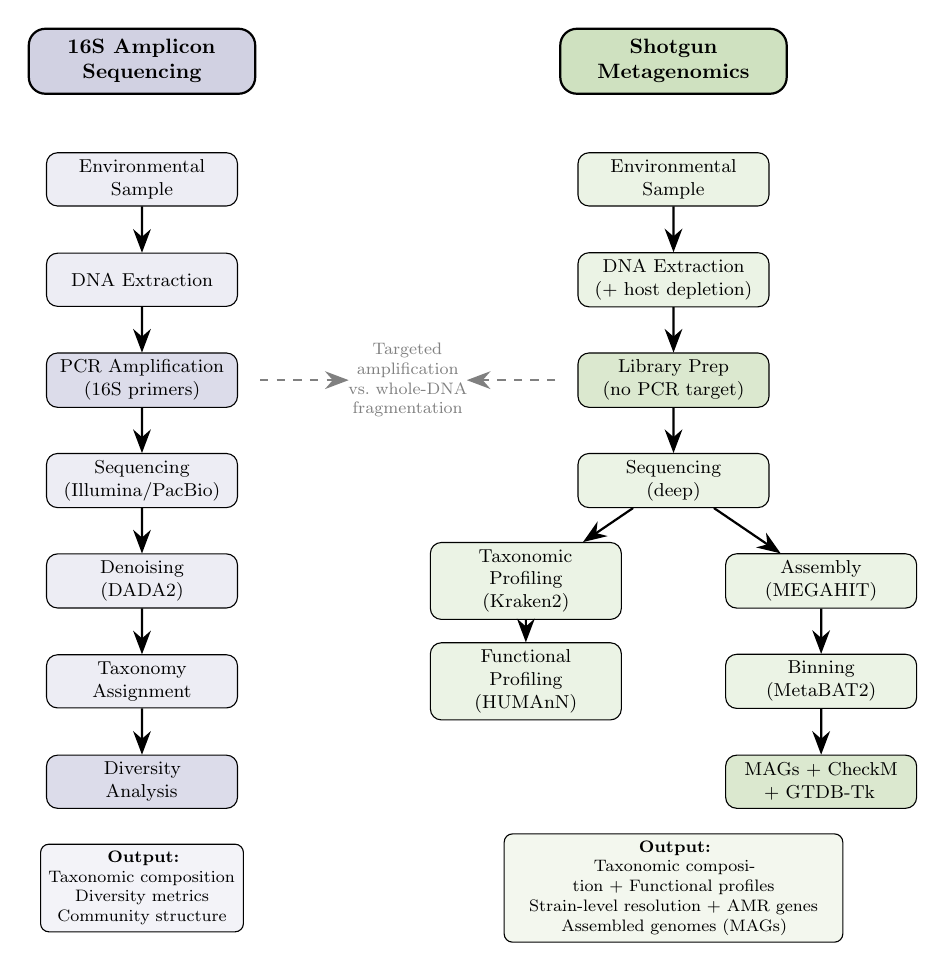
\begin{tikzpicture}[
  scale=0.75,
  transform shape,
  every node/.style={font=\small},
  stepbox/.style={draw, rounded corners=4pt, minimum height=0.9cm, minimum width=3.2cm,
                  text width=3.0cm, align=center, font=\small},
  titlebox/.style={draw, rounded corners=6pt, minimum height=1.1cm, minimum width=3.8cm,
                   text width=3.6cm, align=center, font=\normalsize\bfseries, thick},
  arrow/.style={-{Stealth[length=3mm]}, thick},
  dashed_arrow/.style={-{Stealth[length=3mm]}, thick, dashed, gray},
]

% ---- Amplicon column (left) ----
\node[titlebox, fill=MidnightBlue!20] (amp_title) at (-4.5, 12) {16S Amplicon\\Sequencing};

\node[stepbox, fill=MidnightBlue!8] (amp1) at (-4.5, 10) {Environmental\\Sample};
\node[stepbox, fill=MidnightBlue!8] (amp2) at (-4.5, 8.3) {DNA Extraction};
\node[stepbox, fill=MidnightBlue!15] (amp3) at (-4.5, 6.6) {PCR Amplification\\(16S primers)};
\node[stepbox, fill=MidnightBlue!8] (amp4) at (-4.5, 4.9) {Sequencing\\(Illumina/PacBio)};
\node[stepbox, fill=MidnightBlue!8] (amp5) at (-4.5, 3.2) {Denoising\\(DADA2)};
\node[stepbox, fill=MidnightBlue!8] (amp6) at (-4.5, 1.5) {Taxonomy\\Assignment};
\node[stepbox, fill=MidnightBlue!15] (amp7) at (-4.5, -0.2) {Diversity\\Analysis};

\draw[arrow] (amp1) -- (amp2);
\draw[arrow] (amp2) -- (amp3);
\draw[arrow] (amp3) -- (amp4);
\draw[arrow] (amp4) -- (amp5);
\draw[arrow] (amp5) -- (amp6);
\draw[arrow] (amp6) -- (amp7);

% ---- Shotgun column (right) ----
\node[titlebox, fill=OliveGreen!20] (shot_title) at (4.5, 12) {Shotgun\\Metagenomics};

\node[stepbox, fill=OliveGreen!8] (sh1) at (4.5, 10) {Environmental\\Sample};
\node[stepbox, fill=OliveGreen!8] (sh2) at (4.5, 8.3) {DNA Extraction\\(+ host depletion)};
\node[stepbox, fill=OliveGreen!15] (sh3) at (4.5, 6.6) {Library Prep\\(no PCR target)};
\node[stepbox, fill=OliveGreen!8] (sh4) at (4.5, 4.9) {Sequencing\\(deep)};

% Shotgun branches
\node[stepbox, fill=OliveGreen!8] (sh5a) at (2, 3.2) {Taxonomic\\Profiling\\(Kraken2)};
\node[stepbox, fill=OliveGreen!8] (sh5b) at (7, 3.2) {Assembly\\(MEGAHIT)};

\node[stepbox, fill=OliveGreen!8] (sh6a) at (2, 1.5) {Functional\\Profiling\\(HUMAnN)};
\node[stepbox, fill=OliveGreen!8] (sh6b) at (7, 1.5) {Binning\\(MetaBAT2)};

\node[stepbox, fill=OliveGreen!15] (sh7) at (7, -0.2) {MAGs + CheckM\\+ GTDB-Tk};

\draw[arrow] (sh1) -- (sh2);
\draw[arrow] (sh2) -- (sh3);
\draw[arrow] (sh3) -- (sh4);
\draw[arrow] (sh4) -- (sh5a);
\draw[arrow] (sh4) -- (sh5b);
\draw[arrow] (sh5a) -- (sh6a);
\draw[arrow] (sh5b) -- (sh6b);
\draw[arrow] (sh6b) -- (sh7);

% ---- Comparison annotations ----
\node[font=\footnotesize, text=gray, text width=3.5cm, align=center] at (0, 6.6) {Targeted\\amplification\\vs.\ whole-DNA\\fragmentation};
\draw[dashed_arrow] (-2.5, 6.6) -- (-1, 6.6);
\draw[dashed_arrow] (2.5, 6.6) -- (1, 6.6);

% Output comparison boxes at bottom
\node[draw, rounded corners=3pt, fill=MidnightBlue!5, text width=3.2cm, align=center, font=\footnotesize] at (-4.5, -2) {
  \textbf{Output:}\\
  Taxonomic composition\\
  Diversity metrics\\
  Community structure
};

\node[draw, rounded corners=3pt, fill=OliveGreen!5, text width=5.5cm, align=center, font=\footnotesize] at (4.5, -2) {
  \textbf{Output:}\\
  Taxonomic composition + Functional profiles\\
  Strain-level resolution + AMR genes\\
  Assembled genomes (MAGs)
};

\end{tikzpicture}
\caption{Comparison of 16S amplicon sequencing and shotgun metagenomics workflows. Amplicon sequencing uses targeted PCR amplification of phylogenetic markers, while shotgun metagenomics sequences all DNA, enabling functional profiling, strain-level resolution, and genome-resolved metagenomics.}
\label{fig:amplicon_vs_shotgun}
\end{figure}

%% ============================================================
\section{Comprehensive Tool Comparison}
\label{sec:meta_tool_comparison}
%% ============================================================

\begin{table}[htbp]
\centering
\caption{Comparison of key metagenomics analysis tools by application.}
\label{tab:meta_tools}
\small
\begin{tabularx}{\textwidth}{@{}l*{3}{>{\raggedright\arraybackslash}X}@{}}
\toprule
\textbf{Application} & \textbf{Tool} & \textbf{Approach} & \textbf{Key Features} \\
\midrule
\multirow{2}{*}{Amplicon denoising} & DADA2 & Error model--based denoising & ASV-level resolution, multi-platform \\
 & Deblur & Sequence-error correction & Fast, conservative \\
\addlinespace
\multirow{2}{*}{Amplicon platform} & QIIME 2 & Plugin-based framework & Comprehensive, reproducible, interactive viz \\
 & mothur & Monolithic pipeline & OTU-focused, ecological community \\
\addlinespace
\multirow{3}{*}{Taxonomic profiling} & Kraken2/Bracken & k-mer matching + Bayesian reestimation & Fastest, flexible databases \\
 & MetaPhlAn 4 & Clade-specific markers & High specificity, lower sensitivity \\
 & mOTUs3 & Phylogenetic markers & Detects novel species \\
\addlinespace
\multirow{2}{*}{Functional profiling} & HUMAnN 3 & Species-stratified pathway analysis & Community + species-level functions \\
 & eggNOG-mapper & Orthology-based annotation & Fast, comprehensive \\
\addlinespace
\multirow{2}{*}{Assembly} & MEGAHIT & Succinct DBG, multi-k & Fast, memory-efficient \\
 & MetaSPAdes & Multi-k iterative assembly & Higher contiguity \\
\addlinespace
\multirow{3}{*}{Binning} & MetaBAT2 & TNF + coverage & Fast, automatic \\
 & SemiBin2 & Deep learning embeddings & State-of-the-art accuracy \\
 & DAS Tool & Consensus of multiple binners & Optimised non-redundant bins \\
\addlinespace
\multirow{2}{*}{MAG quality} & CheckM2 & ML-based marker gene analysis & Fast, accurate \\
 & GUNC & Chimerism detection & Catches contamination \\
\addlinespace
\multirow{2}{*}{AMR detection} & CARD/RGI & Curated AMR ontology & Gold standard for AMR \\
 & AMRFinderPlus & HMM + BLAST & NCBI-maintained, comprehensive \\
\bottomrule
\end{tabularx}
\end{table}

%% ============================================================
\section{Practical Workflow: Metagenomics Pipelines}
\label{sec:meta_pipeline}
%% ============================================================

\subsection{Snakemake Shotgun Metagenomics Pipeline}

\begin{lstlisting}[language=Python, caption={Snakemake pipeline for shotgun metagenomics: QC, taxonomic profiling, functional profiling, assembly, and binning.}, label={lst:snakemake_meta}]
# Snakefile for Shotgun Metagenomics Analysis
configfile: "config.yaml"

SAMPLES = config["samples"]
KRAKEN_DB = config["kraken2_db"]
METAPHLAN_DB = config["metaphlan_db"]
REF_HOST = config["host_reference"]  # for host removal

rule all:
    input:
        expand("results/taxonomy/{sample}.kraken2.report",
               sample=SAMPLES),
        expand("results/taxonomy/{sample}.metaphlan.txt",
               sample=SAMPLES),
        expand("results/functional/{sample}_pathabundance.tsv",
               sample=SAMPLES),
        expand("results/mags/{sample}/checkm_results.tsv",
               sample=SAMPLES),
        "results/multiqc/multiqc_report.html"

# --- QC and Host Removal ---
rule fastp_qc:
    input:
        r1="data/fastq/{sample}_R1.fastq.gz",
        r2="data/fastq/{sample}_R2.fastq.gz"
    output:
        r1="results/trimmed/{sample}_R1.trimmed.fastq.gz",
        r2="results/trimmed/{sample}_R2.trimmed.fastq.gz",
        json="results/qc/{sample}.fastp.json",
        html="results/qc/{sample}.fastp.html"
    threads: 4
    shell:
        """
        fastp -i {input.r1} -I {input.r2} \
            -o {output.r1} -O {output.r2} \
            --json {output.json} --html {output.html} \
            --qualified_quality_phred 20 \
            --length_required 50 \
            --thread {threads}
        """

rule remove_host:
    input:
        r1="results/trimmed/{sample}_R1.trimmed.fastq.gz",
        r2="results/trimmed/{sample}_R2.trimmed.fastq.gz",
        ref=REF_HOST
    output:
        r1="results/hostfree/{sample}_R1.fastq.gz",
        r2="results/hostfree/{sample}_R2.fastq.gz"
    threads: 8
    shell:
        """
        bowtie2 -x {input.ref} -1 {input.r1} -2 {input.r2} \
            --very-sensitive -p {threads} \
            --un-conc-gz results/hostfree/{wildcards.sample}_R%.fastq.gz \
            -S /dev/null 2> results/qc/{wildcards.sample}.host_stats.txt
        """

# --- Taxonomic Profiling ---
rule kraken2:
    input:
        r1="results/hostfree/{sample}_R1.fastq.gz",
        r2="results/hostfree/{sample}_R2.fastq.gz"
    output:
        report="results/taxonomy/{sample}.kraken2.report",
        output="results/taxonomy/{sample}.kraken2.output"
    params:
        db=KRAKEN_DB
    threads: 8
    shell:
        """
        kraken2 --db {params.db} \
            --paired {input.r1} {input.r2} \
            --threads {threads} \
            --report {output.report} \
            --output {output.output} \
            --confidence 0.1
        """

rule bracken:
    input:
        report="results/taxonomy/{sample}.kraken2.report"
    output:
        bracken="results/taxonomy/{sample}.bracken.txt"
    params:
        db=KRAKEN_DB
    shell:
        """
        bracken -d {params.db} \
            -i {input.report} \
            -o {output.bracken} \
            -r 150 -l S
        """

rule metaphlan:
    input:
        r1="results/hostfree/{sample}_R1.fastq.gz",
        r2="results/hostfree/{sample}_R2.fastq.gz"
    output:
        profile="results/taxonomy/{sample}.metaphlan.txt"
    params:
        db=METAPHLAN_DB
    threads: 8
    shell:
        """
        metaphlan {input.r1},{input.r2} \
            --input_type fastq \
            --bowtie2db {params.db} \
            --nproc {threads} \
            -o {output.profile}
        """

# --- Functional Profiling ---
rule humann:
    input:
        r1="results/hostfree/{sample}_R1.fastq.gz",
        r2="results/hostfree/{sample}_R2.fastq.gz"
    output:
        genefamilies="results/functional/{sample}_genefamilies.tsv",
        pathabundance="results/functional/{sample}_pathabundance.tsv",
        pathcoverage="results/functional/{sample}_pathcoverage.tsv"
    threads: 8
    shell:
        """
        cat {input.r1} {input.r2} > results/functional/{wildcards.sample}_concat.fastq.gz
        humann --input results/functional/{wildcards.sample}_concat.fastq.gz \
            --output results/functional/{wildcards.sample}_humann/ \
            --threads {threads}
        mv results/functional/{wildcards.sample}_humann/*_genefamilies.tsv \
            {output.genefamilies}
        mv results/functional/{wildcards.sample}_humann/*_pathabundance.tsv \
            {output.pathabundance}
        mv results/functional/{wildcards.sample}_humann/*_pathcoverage.tsv \
            {output.pathcoverage}
        """

# --- Assembly and Binning ---
rule megahit_assembly:
    input:
        r1="results/hostfree/{sample}_R1.fastq.gz",
        r2="results/hostfree/{sample}_R2.fastq.gz"
    output:
        contigs="results/assembly/{sample}/final.contigs.fa"
    threads: 16
    shell:
        """
        megahit -1 {input.r1} -2 {input.r2} \
            -o results/assembly/{wildcards.sample} \
            -t {threads} --min-contig-len 1000
        """

rule map_to_assembly:
    input:
        r1="results/hostfree/{sample}_R1.fastq.gz",
        r2="results/hostfree/{sample}_R2.fastq.gz",
        contigs="results/assembly/{sample}/final.contigs.fa"
    output:
        bam="results/assembly/{sample}/mapped.sorted.bam"
    threads: 8
    shell:
        """
        bowtie2-build {input.contigs} \
            results/assembly/{wildcards.sample}/contigs_idx
        bowtie2 -x results/assembly/{wildcards.sample}/contigs_idx \
            -1 {input.r1} -2 {input.r2} \
            -p {threads} --very-sensitive \
        | samtools sort -@ 4 -o {output.bam} -
        samtools index {output.bam}
        """

rule metabat2_binning:
    input:
        contigs="results/assembly/{sample}/final.contigs.fa",
        bam="results/assembly/{sample}/mapped.sorted.bam"
    output:
        bins=directory("results/mags/{sample}/bins")
    threads: 8
    shell:
        """
        jgi_summarize_bam_contig_depths --outputDepth \
            results/mags/{wildcards.sample}/depth.txt {input.bam}
        metabat2 -i {input.contigs} \
            -a results/mags/{wildcards.sample}/depth.txt \
            -o {output.bins}/bin \
            -t {threads} --minContig 1500
        """

rule checkm:
    input:
        bins="results/mags/{sample}/bins"
    output:
        results="results/mags/{sample}/checkm_results.tsv"
    threads: 8
    shell:
        """
        checkm2 predict \
            --input {input.bins} \
            --output-directory results/mags/{wildcards.sample}/checkm \
            --threads {threads} -x fa
        cp results/mags/{wildcards.sample}/checkm/quality_report.tsv \
            {output.results}
        """

rule multiqc:
    input:
        expand("results/qc/{sample}.fastp.json", sample=SAMPLES)
    output:
        "results/multiqc/multiqc_report.html"
    shell:
        """
        multiqc results/qc/ -o results/multiqc/ --force
        """
\end{lstlisting}

\subsection{Nextflow Shotgun Metagenomics Pipeline}

\begin{lstlisting}[language=Java, caption={Nextflow DSL2 pipeline for shotgun metagenomics analysis.}, label={lst:nextflow_meta}]
#!/usr/bin/env nextflow
nextflow.enable.dsl=2

// Shotgun Metagenomics Analysis Pipeline

params.reads      = "data/fastq/*_{R1,R2}.fastq.gz"
params.host_ref   = "reference/human_bowtie2_idx"
params.kraken_db  = "databases/kraken2_standard"
params.outdir     = "results"

process FASTP {
    tag "$sample_id"
    publishDir "${params.outdir}/trimmed", mode: 'copy'
    cpus 4

    input:
    tuple val(sample_id), path(reads)

    output:
    tuple val(sample_id),
          path("${sample_id}_R{1,2}.trimmed.fastq.gz"),
          emit: trimmed
    path("${sample_id}.fastp.json"), emit: report

    script:
    """
    fastp -i ${reads[0]} -I ${reads[1]} \
        -o ${sample_id}_R1.trimmed.fastq.gz \
        -O ${sample_id}_R2.trimmed.fastq.gz \
        --json ${sample_id}.fastp.json \
        --qualified_quality_phred 20 \
        --length_required 50 \
        --thread ${task.cpus}
    """
}

process REMOVE_HOST {
    tag "$sample_id"
    publishDir "${params.outdir}/hostfree", mode: 'copy'
    cpus 8

    input:
    tuple val(sample_id), path(reads)
    path host_idx

    output:
    tuple val(sample_id),
          path("${sample_id}_R{1,2}.hostfree.fastq.gz"),
          emit: hostfree

    script:
    """
    bowtie2 -x ${host_idx}/genome \
        -1 ${reads[0]} -2 ${reads[1]} \
        --very-sensitive -p ${task.cpus} \
        --un-conc-gz ${sample_id}_R%.hostfree.fastq.gz \
        -S /dev/null
    """
}

process KRAKEN2 {
    tag "$sample_id"
    publishDir "${params.outdir}/taxonomy", mode: 'copy'
    cpus 8

    input:
    tuple val(sample_id), path(reads)
    path kraken_db

    output:
    tuple val(sample_id),
          path("${sample_id}.kraken2.report"),
          emit: kraken_report
    path("${sample_id}.kraken2.output"), emit: kraken_out

    script:
    """
    kraken2 --db ${kraken_db} \
        --paired ${reads[0]} ${reads[1]} \
        --threads ${task.cpus} \
        --report ${sample_id}.kraken2.report \
        --output ${sample_id}.kraken2.output \
        --confidence 0.1
    """
}

process BRACKEN {
    tag "$sample_id"
    publishDir "${params.outdir}/taxonomy", mode: 'copy'

    input:
    tuple val(sample_id), path(kraken_report)
    path kraken_db

    output:
    tuple val(sample_id),
          path("${sample_id}.bracken.txt"),
          emit: bracken_out

    script:
    """
    bracken -d ${kraken_db} \
        -i ${kraken_report} \
        -o ${sample_id}.bracken.txt \
        -r 150 -l S
    """
}

process MEGAHIT {
    tag "$sample_id"
    publishDir "${params.outdir}/assembly", mode: 'copy'
    cpus 16
    memory '32 GB'

    input:
    tuple val(sample_id), path(reads)

    output:
    tuple val(sample_id),
          path("${sample_id}_contigs.fa"),
          emit: contigs

    script:
    """
    megahit -1 ${reads[0]} -2 ${reads[1]} \
        -o megahit_out -t ${task.cpus} \
        --min-contig-len 1000
    mv megahit_out/final.contigs.fa ${sample_id}_contigs.fa
    """
}

process MAP_READS {
    tag "$sample_id"
    publishDir "${params.outdir}/mapped", mode: 'copy'
    cpus 8

    input:
    tuple val(sample_id), path(reads), path(contigs)

    output:
    tuple val(sample_id), path(contigs),
          path("${sample_id}.sorted.bam"),
          path("${sample_id}.sorted.bam.bai"),
          emit: mapped

    script:
    """
    bowtie2-build ${contigs} contigs_idx
    bowtie2 -x contigs_idx \
        -1 ${reads[0]} -2 ${reads[1]} \
        -p ${task.cpus} --very-sensitive \
    | samtools sort -@ 4 -o ${sample_id}.sorted.bam -
    samtools index ${sample_id}.sorted.bam
    """
}

process METABAT2 {
    tag "$sample_id"
    publishDir "${params.outdir}/mags", mode: 'copy'
    cpus 8

    input:
    tuple val(sample_id), path(contigs),
          path(bam), path(bai)

    output:
    tuple val(sample_id),
          path("${sample_id}_bins/"),
          emit: bins

    script:
    """
    mkdir -p ${sample_id}_bins
    jgi_summarize_bam_contig_depths \
        --outputDepth depth.txt ${bam}
    metabat2 -i ${contigs} -a depth.txt \
        -o ${sample_id}_bins/bin \
        -t ${task.cpus} --minContig 1500
    """
}

process CHECKM2 {
    tag "$sample_id"
    publishDir "${params.outdir}/mags/quality", mode: 'copy'
    cpus 8

    input:
    tuple val(sample_id), path(bins)

    output:
    tuple val(sample_id),
          path("${sample_id}_checkm.tsv"),
          emit: quality

    script:
    """
    checkm2 predict \
        --input ${bins} \
        --output-directory checkm_out \
        --threads ${task.cpus} -x fa
    cp checkm_out/quality_report.tsv ${sample_id}_checkm.tsv
    """
}

// ---- Workflow ----
workflow {
    Channel
        .fromFilePairs(params.reads)
        .set { reads_ch }

    host_ref  = file(params.host_ref)
    kraken_db = file(params.kraken_db)

    // QC and host removal
    FASTP(reads_ch)
    REMOVE_HOST(FASTP.out.trimmed, host_ref)

    // Taxonomic profiling
    KRAKEN2(REMOVE_HOST.out.hostfree, kraken_db)
    BRACKEN(KRAKEN2.out.kraken_report, kraken_db)

    // Assembly and binning
    MEGAHIT(REMOVE_HOST.out.hostfree)

    // Combine hostfree reads with contigs for mapping
    map_input = REMOVE_HOST.out.hostfree
        .join(MEGAHIT.out.contigs)
        .map { id, reads, contigs ->
            tuple(id, reads, contigs)
        }

    MAP_READS(map_input)
    METABAT2(MAP_READS.out.mapped)
    CHECKM2(METABAT2.out.bins)
}
\end{lstlisting}

\begin{protocolbox}[title={Community-Curated Metagenomics Pipelines}]
Several community-maintained pipelines implement best-practice metagenomics workflows:
\begin{itemize}[nosep]
  \item \textbf{nf-core/ampliseq}: Nextflow pipeline for amplicon sequencing (16S, 18S, ITS) with DADA2 and QIIME 2 integration.
  \item \textbf{nf-core/mag}: Nextflow pipeline for metagenome assembly, binning, and MAG analysis with comprehensive quality assessment.
  \item \textbf{nf-core/taxprofiler}: Nextflow pipeline for multi-tool taxonomic profiling (Kraken2, MetaPhlAn, mOTUs, Centrifuge, and more) with standardised outputs.
  \item \textbf{Sunbeam}: Snakemake-based extensible metagenomics pipeline with QC, host removal, assembly, and annotation.
  \item \textbf{Atlas}: Snakemake-based metagenome pipeline for assembly, binning, and annotation.
\end{itemize}
These pipelines handle edge cases, provide extensive QC reports, and are continuously tested---consider using them before building custom pipelines.
\end{protocolbox}

%% ============================================================
\section{Long-Read Metagenomics Workflow Considerations}
\label{sec:longread_meta_workflow}
%% ============================================================

For long-read metagenomic experiments, the analysis workflow differs in several key ways:

\begin{enumerate}[nosep]
  \item \textbf{QC}: Use \software{NanoPlot} for ONT quality assessment, \software{chopper} or \software{Filtlong} for quality and length filtering. For PacBio HiFi, use \software{pbccs} and quality filtering is minimal (already high accuracy).
  \item \textbf{Taxonomic classification}: \software{Kraken2} works well with long reads. \software{Centrifuge} and \software{Emu} (designed specifically for full-length 16S long reads) are alternatives.
  \item \textbf{Assembly}: \software{metaFlye} for ONT data; \software{hifiasm-meta} for PacBio HiFi metagenomes. Long reads typically produce far more contiguous assemblies with higher N50.
  \item \textbf{Binning}: Standard binners (MetaBAT2, SemiBin2) work, but methylation-aware binning (\software{bin\_reassigner}) can dramatically improve results for ONT and PacBio data by using epigenetic signatures as an additional binning signal.
  \item \textbf{Polishing}: ONT assemblies may benefit from short-read polishing with \software{Pilon} or \software{Polypolish} to improve consensus accuracy.
\end{enumerate}

%% ============================================================
\section{Summary}
\label{sec:ch09_summary}
%% ============================================================

\begin{keyconcept}[title={Chapter Summary}]
\begin{itemize}[nosep]
  \item \textbf{Metagenomics} bypasses culturing to study all microorganisms in a sample, revolutionising our understanding of microbial communities in health, disease, and the environment.
  \item \textbf{16S amplicon sequencing} is cost-effective for community composition profiling using conserved marker genes. The \textbf{ASV} approach (DADA2) has replaced OTU clustering as the standard for sequence resolution.
  \item \textbf{Shotgun metagenomics} provides a comprehensive view: taxonomic profiling across all domains of life (\software{Kraken2}, \software{MetaPhlAn}), functional potential (\software{HUMAnN}), strain-level resolution, and \textbf{metagenome-assembled genomes (MAGs)} from assembly and binning.
  \item \textbf{MAG quality} is assessed using \software{CheckM2} and classified using \software{GTDB-Tk}, following MIMAG standards for completeness and contamination.
  \item \textbf{Clinical metagenomics} enables unbiased pathogen detection and \textbf{AMR gene surveillance}, with databases such as CARD, ResFinder, and AMRFinderPlus.
  \item \textbf{Diversity analysis} uses alpha metrics (Shannon, Simpson, Chao1), beta metrics (Bray-Curtis, UniFrac), and ordination (PCoA, NMDS) to characterise and compare communities.
  \item \textbf{Long-read metagenomics} (full-length 16S, nanopore adaptive sampling, methylation-aware binning) is rapidly improving resolution and enabling genome-resolved metagenomics from complex environments.
  \item Both \textbf{Snakemake} and \textbf{Nextflow} provide robust workflow frameworks, with community pipelines (\software{nf-core/mag}, \software{nf-core/ampliseq}) available for immediate adoption.
\end{itemize}
\end{keyconcept}


% Part IV: Transcriptomics
\part{Transcriptomics: Gene Expression and RNA Biology}
% ==============================================================================
% Chapter 10: RNA Sequencing — Measuring Gene Expression
% ==============================================================================
\chapter{RNA Sequencing: Measuring Gene Expression}
\label{ch:rnaseq}

\begin{keyconcept}
RNA sequencing (\acrshort{RNA-seq}) measures the transcriptome---the complete set of RNA
transcripts in a cell, tissue, or organism at a given moment. Because gene
expression is the primary mechanism through which genotype becomes phenotype,
\acrshort{RNA-seq} has become one of the most widely used sequencing applications in
biology and medicine.
\end{keyconcept}

% ---------------------------------------------------------------------------
\section{Why Measure RNA?}
\label{sec:rnaseq:why}

Every cell in a multicellular organism carries essentially the same genome, yet
a neuron looks and behaves nothing like a hepatocyte. The difference lies
predominantly in \emph{which genes are expressed} and at \emph{what levels}.
Measuring RNA therefore provides a direct readout of cellular state.

\subsection{Gene Expression as a Window into Biology}

Gene expression governs virtually every biological process:

\begin{itemize}[nosep]
  \item \textbf{Development.} Transcription factors activate stage-specific
    gene programs that drive differentiation from a single zygote into hundreds
    of specialized cell types.
  \item \textbf{Disease.} Cancers are defined by aberrant expression profiles;
    autoimmune diseases by dysregulated immune genes; neurodegeneration by
    altered synaptic gene networks.
  \item \textbf{Environmental response.} Cells respond to stress, infection,
    drugs, and nutrients by rapidly reprogramming their transcriptomes.
  \item \textbf{Circadian rhythm.} Thousands of genes oscillate with 24-hour
    periodicity in virtually every tissue.
\end{itemize}

Before \acrshort{RNA-seq}, gene expression was measured by microarrays,
Northern blots, or quantitative PCR (qPCR). Microarrays could interrogate
thousands of genes simultaneously but relied on predefined probes, suffered
from cross-hybridization, and had limited dynamic range. \acrshort{RNA-seq}
overcame all of these limitations: it is unbiased, quantitative across
five orders of magnitude, and can detect novel transcripts, splice variants,
and allele-specific expression without any prior knowledge of the genome.

\subsection{The Transcriptome}

The transcriptome is far more complex than a simple catalogue of protein-coding
messenger RNAs:

\begin{description}[style=nextline]
  \item[Messenger RNA (mRNA)] Protein-coding transcripts, accounting for only
    $\sim$2--5\% of total RNA mass but $\sim$20,000 genes in humans.
  \item[Ribosomal RNA (rRNA)] The dominant RNA species by mass ($\sim$80--85\%),
    forming the structural and catalytic core of ribosomes (28S, 18S, 5.8S, 5S
    in eukaryotes).
  \item[Transfer RNA (tRNA)] Adapter molecules ($\sim$10--15\% of RNA) that
    deliver amino acids during translation.
  \item[Long non-coding RNA (lncRNA)] Transcripts $>$200\,nt that do not encode
    proteins; $>$60,000 annotated in humans. Functions include chromatin
    remodeling, transcriptional regulation, and scaffolding (e.g., \gene{XIST},
    \gene{MALAT1}, \gene{HOTAIR}).
  \item[Small non-coding RNAs] Include microRNAs (miRNAs, $\sim$22\,nt),
    piwi-interacting RNAs (piRNAs, 24--32\,nt), small interfering RNAs
    (siRNAs), small nucleolar RNAs (snoRNAs), and tRNA-derived fragments
    (tRFs).
  \item[Circular RNAs (circRNAs)] Covalently closed loops formed by
    back-splicing; highly stable, tissue-specific, and implicated in miRNA
    sponging and translation regulation.
  \item[Transcript isoforms] Alternative splicing, alternative polyadenylation,
    and alternative transcription start sites generate multiple isoforms per
    gene. Human genes produce an average of $\sim$7 distinct isoforms.
\end{description}

\begin{warningbox}
The vast majority of cellular RNA is ribosomal RNA. Without an enrichment or
depletion strategy, an \acrshort{RNA-seq} experiment would waste $>$80\% of
sequencing reads on rRNA.
\end{warningbox}


% ---------------------------------------------------------------------------
\section{Bulk RNA-seq: An Overview of Approaches}
\label{sec:rnaseq:bulk}

Bulk \acrshort{RNA-seq} measures the \emph{average} expression across a
population of cells (typically $10^5$--$10^7$ cells). Two main strategies exist,
distinguished by how they deal with the rRNA problem.

\subsection{mRNA-seq: Poly-A Selection}

The most common approach for studying protein-coding gene expression.
Polyadenylated transcripts (mRNAs plus some lncRNAs) are captured using
oligo-dT beads that hybridize to the poly-A tail.

\begin{protocolbox}[title={Poly-A Selection Protocol Overview}]
\begin{enumerate}[nosep]
  \item Extract total RNA (e.g., TRIzol or column-based methods).
  \item Incubate with oligo-dT magnetic beads; poly-A$^+$ transcripts bind.
  \item Wash away rRNA, tRNA, and other non-polyadenylated RNAs.
  \item Elute mRNA and proceed to fragmentation and cDNA synthesis.
\end{enumerate}
Requires high-quality RNA with intact poly-A tails (RIN $\geq$ 7 recommended).
\end{protocolbox}

\textbf{Advantages:}
\begin{itemize}[nosep]
  \item Highly enriched for protein-coding transcripts.
  \item Lower sequencing depth required (fewer ``wasted'' reads).
  \item Well-established, widely used---most public datasets use this approach.
\end{itemize}

\textbf{Limitations:}
\begin{itemize}[nosep]
  \item Misses non-polyadenylated transcripts (histone mRNAs, many lncRNAs, most
    small RNAs, bacterial transcripts).
  \item Requires high-quality RNA; degraded samples lose poly-A tails, biasing
    toward 3$'$ ends.
  \item Cannot capture nascent or nuclear RNA species lacking poly-A tails.
\end{itemize}

\subsection{Total RNA-seq: Ribosomal RNA Depletion}

Ribosomal depletion removes rRNA from total RNA, leaving all other RNA species
intact---mRNAs, lncRNAs, circRNAs, pre-mRNAs, and other non-coding species.

Common rRNA depletion kits include:
\begin{itemize}[nosep]
  \item \textbf{Illumina Ribo-Zero Plus:} uses DNA probe hybridization and
    RNase H digestion to deplete rRNA from human, mouse, rat, and bacterial
    samples.
  \item \textbf{RiboCop (Lexogen):} enzymatic rRNA depletion compatible with
    degraded samples.
  \item \textbf{NEBNext rRNA Depletion Kit:} probe-based depletion for human,
    mouse, and rat.
  \item \textbf{QIAseq FastSelect:} targets rRNA during reverse transcription,
    eliminating a separate depletion step.
\end{itemize}

\textbf{Advantages:}
\begin{itemize}[nosep]
  \item Captures both coding and non-coding RNA.
  \item Works with degraded/FFPE samples (no reliance on poly-A tail integrity).
  \item Detects intronic reads, pre-mRNAs, and nascent transcription signals.
  \item Can reveal circular RNAs (which lack poly-A tails).
\end{itemize}

\textbf{Limitations:}
\begin{itemize}[nosep]
  \item Residual rRNA ($\sim$1--10\%) consumes some sequencing capacity.
  \item More complex read composition; requires deeper sequencing for equivalent
    mRNA coverage.
  \item May require organism-specific depletion probes for non-model organisms.
\end{itemize}

\subsection{Choosing Between mRNA-seq and Total RNA-seq}

\begin{table}[htbp]
\centering
\caption{Comparison of mRNA-seq (poly-A selection) and total RNA-seq (rRNA
depletion) approaches.}
\label{tab:rnaseq:mrna_vs_total}
\small
\begin{tabularx}{\textwidth}{lXX}
\toprule
\textbf{Feature} & \textbf{mRNA-seq (poly-A)} & \textbf{Total RNA-seq (rRNA depletion)} \\
\midrule
Target RNA & Poly-A$^+$ mRNA (+ some lncRNA) & All RNA except rRNA \\
RNA quality requirement & High (RIN $\geq$ 7) & Moderate (works with RIN $\geq$ 2) \\
FFPE samples & Poor performance & Suitable \\
Non-coding RNA & Missed (most) & Captured \\
Intronic reads & Minimal & Substantial \\
Circular RNA & Not captured & Captured \\
Typical depth needed & 20--30M reads & 40--60M reads \\
Cost per informative read & Lower & Higher \\
Best for & Standard differential expression & Degraded samples, ncRNA, comprehensive profiling \\
\bottomrule
\end{tabularx}
\end{table}

\begin{tipbox}
If your primary goal is differential expression of protein-coding genes and your
RNA quality is good (RIN $\geq$ 7), mRNA-seq is the most cost-effective choice.
If you are working with clinical/FFPE samples, interested in non-coding RNAs, or
need to capture the broadest possible transcriptome, use total RNA-seq.
\end{tipbox}


% ---------------------------------------------------------------------------
\section{Library Preparation for RNA-seq}
\label{sec:rnaseq:library}

\subsection{RNA Extraction and Quality Assessment}

High-quality RNA is the single most critical determinant of a successful
\acrshort{RNA-seq} experiment. RNA is chemically fragile and ubiquitous RNases
in the environment degrade it rapidly.

\begin{description}[style=nextline]
  \item[Extraction methods]
    \begin{itemize}[nosep]
      \item \textbf{TRIzol / TRI Reagent:} acid guanidinium--phenol--chloroform
        extraction. Gold standard for yield; suitable for most tissues.
      \item \textbf{Column-based:} RNeasy (Qiagen), PureLink (Invitrogen). Faster,
        less toxic, but lower yield for difficult tissues.
      \item \textbf{Automated:} KingFisher (Thermo), QIAsymphony. Essential for
        high-throughput core facilities.
    \end{itemize}
  \item[Quality metrics]
    \begin{itemize}[nosep]
      \item \textbf{RIN (RNA Integrity Number):} Agilent Bioanalyzer / TapeStation
        score from 1 (fully degraded) to 10 (intact). Based on the 28S/18S rRNA
        ratio and the electropherogram trace. RIN $\geq$ 7 is recommended for
        poly-A selection.
      \item \textbf{DV200:} Fraction of RNA fragments $>$ 200 nucleotides.
        Preferred metric for degraded/FFPE RNA because the RIN algorithm
        performs poorly when rRNA peaks are absent. DV200 $\geq$ 30\% is
        often the minimum for library construction with specialized FFPE kits.
      \item \textbf{Concentration:} Qubit fluorometer (RNA HS Assay) provides
        accurate quantitation; NanoDrop UV absorbance gives purity ratios
        (260/280 $\sim$ 2.0 for pure RNA; 260/230 $\geq$ 1.8).
    \end{itemize}
\end{description}

\subsection{Strand-Specific Library Preparation}
\label{sec:rnaseq:stranded}

In unstranded \acrshort{RNA-seq}, the original strand of the RNA transcript
cannot be determined from the sequencing reads. Strand-specific (stranded)
protocols preserve this information.

\subsubsection{Why Strandedness Matters}

\begin{itemize}[nosep]
  \item \textbf{Overlapping genes:} In complex genomes, genes on opposite
    strands can overlap. Unstranded data cannot assign reads to the correct
    gene.
  \item \textbf{Antisense transcription:} Many loci produce antisense
    transcripts that regulate the sense gene. Without strand information, sense
    and antisense reads are indistinguishable.
  \item \textbf{Accurate quantification:} Stranded data improves the accuracy
    of gene-level and transcript-level quantification by 5--15\% for
    overlapping annotations.
  \item \textbf{Novel transcript discovery:} Strand information is essential
    for correctly assembling and annotating novel transcripts.
\end{itemize}

\subsubsection{The dUTP Method}

The most widely used strand-specific protocol:

\begin{enumerate}[nosep]
  \item Fragment mRNA and synthesize first-strand cDNA using random primers.
  \item Synthesize second-strand cDNA incorporating dUTP instead of dTTP.
  \item Ligate sequencing adapters.
  \item Digest the dUTP-containing second strand with USER enzyme (uracil-DNA
    glycosylase + endonuclease VIII).
  \item Only the first-strand cDNA (complementary to the original mRNA) is
    amplified and sequenced.
  \item Read 2 corresponds to the sense strand of the original mRNA.
\end{enumerate}

This is the basis of the \textbf{Illumina Stranded mRNA Prep} and
\textbf{Illumina Stranded Total RNA Prep} kits, which have largely become the
community standard.

% TikZ diagram: Strand-specific library prep
\begin{figure}[htbp]
\centering
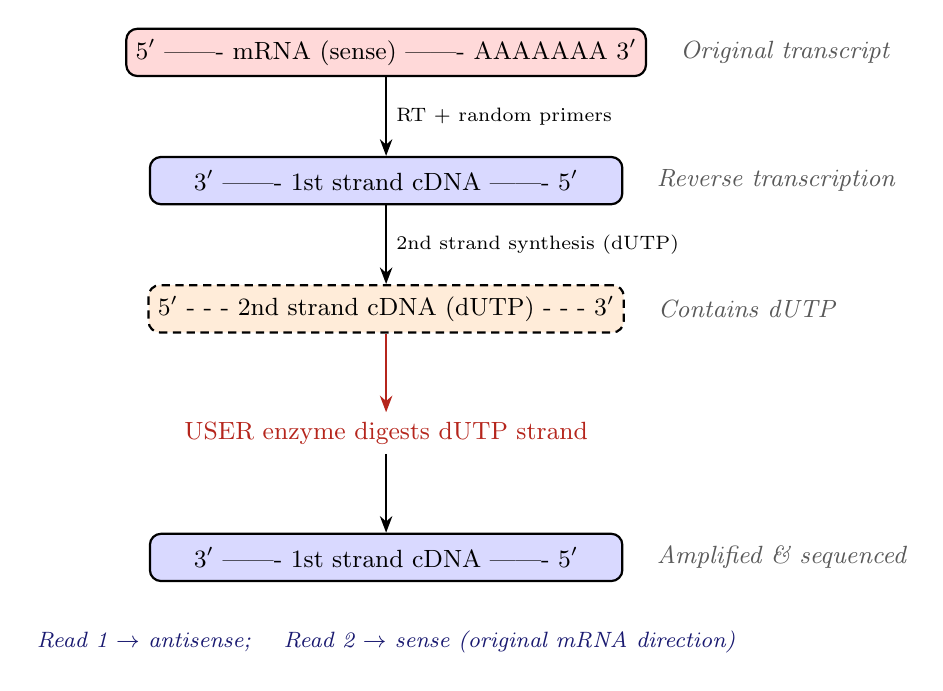
\begin{tikzpicture}[
  node distance=0.7cm,
  every node/.style={font=\small},
  rna/.style={draw, thick, fill=red!15, rounded corners, minimum width=6cm, minimum height=0.6cm},
  cdna1/.style={draw, thick, fill=blue!15, rounded corners, minimum width=6cm, minimum height=0.6cm},
  cdna2/.style={draw, thick, fill=orange!15, rounded corners, minimum width=6cm, minimum height=0.6cm, densely dashed},
  arrow/.style={-{Stealth[length=6pt]}, thick},
  label/.style={font=\small\itshape, text=gray!70!black}
]

% Step 1: mRNA
\node[rna] (mrna) {5$'$ ------- mRNA (sense) ------- AAAAAAA 3$'$};
\node[label, right=0.3cm of mrna] {Original transcript};

% Step 2: First-strand cDNA
\node[cdna1, below=1.0cm of mrna] (ss1) {3$'$ ------- 1st strand cDNA ------- 5$'$};
\node[label, right=0.3cm of ss1] {Reverse transcription};
\draw[arrow] (mrna.south) -- node[right, font=\scriptsize] {RT + random primers} (ss1.north);

% Step 3: Second-strand with dUTP
\node[cdna2, below=1.0cm of ss1] (ss2) {5$'$ - - - 2nd strand cDNA (dUTP) - - - 3$'$};
\node[label, right=0.3cm of ss2] {Contains dUTP};
\draw[arrow] (ss1.south) -- node[right, font=\scriptsize] {2nd strand synthesis (dUTP)} (ss2.north);

% Step 4: USER enzyme digestion
\node[below=1.0cm of ss2, font=\small, text=BrickRed] (digest) {USER enzyme digests dUTP strand};
\draw[arrow, BrickRed] (ss2.south) -- (digest.north);

% Step 5: Only first strand remains
\node[cdna1, below=1.0cm of digest] (final) {3$'$ ------- 1st strand cDNA ------- 5$'$};
\node[label, right=0.3cm of final] {Amplified \& sequenced};
\draw[arrow] (digest.south) -- (final.north);

% Annotation
\node[below=0.5cm of final, font=\footnotesize\itshape, text=MidnightBlue] {Read 1 $\rightarrow$ antisense; \quad Read 2 $\rightarrow$ sense (original mRNA direction)};

\end{tikzpicture}
\caption{Schematic of the dUTP strand-specific library preparation method. The
second-strand cDNA is synthesized with dUTP (dashed orange) and subsequently
digested by USER enzyme, ensuring that only the first-strand cDNA (blue) is
amplified. This preserves strand-of-origin information.}
\label{fig:rnaseq:stranded}
\end{figure}

\subsection{Low-Input RNA-seq}

Standard RNA-seq protocols require 100\,ng--1\,$\mu$g of total RNA. Many
biological questions demand profiling from small cell populations, sorted cells,
or limited clinical material.

\begin{description}[style=nextline]
  \item[Smart-seq2] Full-length transcript coverage from single cells or
    picogram-level input. Uses template-switching oligos and limited PCR
    amplification. Plate-based (typically 96- or 384-well). Excellent
    sensitivity but low throughput and not strand-specific in the original
    protocol.
  \item[SMART-Seq Stranded (Takara)] Combines Smart-seq template-switching
    with strand-specific library prep. Input as low as 10\,pg (single cells)
    to 10\,ng. Adds strand specificity lacking in original Smart-seq2.
  \item[NEBNext Single Cell / Low Input RNA Library Prep] Template-switching
    approach compatible with 2\,pg--200\,ng input.
\end{description}

\subsection{Degraded RNA and FFPE Samples}

Formalin-fixed paraffin-embedded (FFPE) tissues are ubiquitous in pathology
archives. The fixation and embedding process crosslinks and fragments RNA
severely (RIN typically 1--3). Specialized protocols are needed:

\begin{itemize}[nosep]
  \item \textbf{Illumina Stranded Total RNA with Ribo-Zero Plus:} works with
    FFPE RNA down to DV200 of $\sim$30\%.
  \item \textbf{KAPA RNA HyperPrep with RiboErase:} optimized for low-quality
    input; produces libraries from as little as 25\,ng FFPE RNA.
  \item \textbf{Takara SMARTer Stranded Total RNA-Seq Kit v3 -- Pico Input:}
    designed for 250\,pg--10\,ng of degraded RNA.
  \item \textbf{Probe-based approaches (Twist Bioscience RNA Panel, IDT xGen
    RNA):} use hybridization capture for targeted RNA panels from FFPE
    samples.
\end{itemize}

\begin{warningbox}
FFPE RNA-seq data has distinct characteristics: shorter insert sizes, higher
duplicate rates, and 3$'$ bias. Specialized QC metrics (DV200, percentage of
reads in gene bodies) should be used. The standard RIN score is unreliable for
FFPE samples.
\end{warningbox}


% ---------------------------------------------------------------------------
\section{Small RNA Sequencing}
\label{sec:rnaseq:smallrna}

Small RNA-seq targets RNA molecules $<$ 200\,nt, with a particular focus on
microRNAs (miRNAs, $\sim$22\,nt), which are key post-transcriptional
regulators of gene expression.

\subsection{Small RNA Species}

\begin{description}[style=nextline]
  \item[microRNAs (miRNAs)] 19--25\,nt single-stranded RNAs that bind the
    3$'$ UTR of target mRNAs to induce translational repression or mRNA
    degradation. $\sim$2,600 mature miRNAs annotated in humans (miRBase v22.1).
  \item[piRNAs] 24--32\,nt RNAs that silence transposable elements in the
    germline; associate with PIWI-clade Argonaute proteins.
  \item[siRNAs] 20--24\,nt double-stranded RNA-derived species involved in RNA
    interference.
  \item[tRNA-derived fragments (tRFs)] 14--35\,nt fragments cleaved from mature
    or precursor tRNAs. Emerging roles in stress response, gene regulation,
    and cancer.
  \item[snoRNAs] 60--300\,nt; guide chemical modifications of rRNA and snRNA.
\end{description}

\subsection{Small RNA Library Preparation}

\begin{protocolbox}[title={Small RNA-seq Library Preparation}]
\begin{enumerate}[nosep]
  \item \textbf{Size selection:} Total RNA is size-selected for 15--50\,nt
    fragments using PAGE gel or bead-based selection.
  \item \textbf{3$'$ adapter ligation:} An adapter is ligated to the 3$'$-OH of
    small RNAs (which have a free 3$'$-OH after Dicer processing).
  \item \textbf{5$'$ adapter ligation:} An adapter is ligated to the 5$'$
    phosphate.
  \item \textbf{Reverse transcription:} cDNA is synthesized from the
    adapter-ligated small RNA.
  \item \textbf{PCR amplification:} Limited-cycle PCR with indexed primers.
  \item \textbf{Size selection:} Final library is size-selected ($\sim$135--170\,bp
    including adapters) to remove adapter dimers.
\end{enumerate}
\end{protocolbox}

\begin{warningbox}[title={Adapter Dimers in Small RNA-seq}]
Adapter dimers (3$'$ and 5$'$ adapters ligated directly to each other without
a small RNA insert) are the most common artifact in small RNA-seq. They are
$\sim$120--130\,bp and can dominate the library if input RNA is limiting.
Rigorous gel-based or bead-based size selection is essential. Always check the
library size distribution on a Bioanalyzer/TapeStation before sequencing.
\end{warningbox}

\subsection{miRNA-seq Analysis Workflow}

The analysis of miRNA-seq data follows a specialized pipeline:

\begin{enumerate}[nosep]
  \item \textbf{Adapter trimming:} Critical because inserts ($\sim$22\,nt)
    are shorter than reads (typically 50--75\,bp). Tools: \software{Cutadapt},
    \software{Trim Galore}, \software{fastp}.
  \item \textbf{Quality filtering:} Remove reads $<$ 15\,nt or $>$ 35\,nt after
    trimming.
  \item \textbf{Mapping to miRNA reference:} Align to mature and precursor miRNA
    sequences from miRBase using \software{Bowtie} (allowing 0--1 mismatches)
    or dedicated tools.
  \item \textbf{Quantification:} Count reads mapping to each miRNA.
  \item \textbf{Normalization and differential expression:} Use
    \software{DESeq2} or \software{edgeR} as for mRNA, but with miRNA-specific
    considerations (lower library complexity, more discrete count
    distributions).
  \item \textbf{Target prediction:} \software{TargetScan}, \software{miRDB},
    \software{DIANA-microT}.
\end{enumerate}

Key tools for small RNA analysis include:
\begin{itemize}[nosep]
  \item \textbf{miRDeep2:} Discovers known and novel miRNAs by modeling the
    miRNA biogenesis pathway (Drosha/Dicer processing signatures).
  \item \textbf{sRNAbench:} Comprehensive small RNA analysis including miRNA,
    piRNA, tRFs, and isomiR detection.
  \item \textbf{miRge 3.0:} Fast miRNA alignment and quantification using a
    Bayesian approach.
  \item \textbf{Oasis 2.0:} Web-based platform for small RNA-seq analysis.
\end{itemize}


% ---------------------------------------------------------------------------
\section{Long-Read RNA Sequencing}
\label{sec:rnaseq:longread}

Short-read RNA-seq excels at quantification but struggles with isoform
resolution. When multiple transcript isoforms share exons, short reads
($\sim$150\,bp) cannot span the full transcript, making it impossible to
determine which combination of exons belongs to the same molecule. Long-read
RNA sequencing solves this by reading full-length transcripts.

\subsection{PacBio Iso-Seq}

The \textbf{Isoform Sequencing (Iso-Seq)} protocol from Pacific Biosciences
produces full-length transcript sequences without the need for assembly:

\begin{enumerate}[nosep]
  \item Reverse-transcribe poly-A$^+$ RNA into full-length cDNA using a
    template-switching oligo.
  \item Size-select cDNA (optional; can fractionate to enrich specific size
    ranges).
  \item Generate SMRTbell libraries and sequence on the PacBio Revio or Sequel
    IIe platform.
  \item Use the \software{IsoSeq3} pipeline to produce high-quality (HQ)
    full-length transcript isoforms with $>$99\% accuracy using CCS reads.
\end{enumerate}

Typical output: 5--15 million HiFi reads per SMRT Cell on Revio, yielding
hundreds of thousands of unique transcript isoforms.

\subsection{Oxford Nanopore RNA Sequencing}

Oxford Nanopore offers two RNA-seq approaches:

\begin{description}[style=nextline]
  \item[Direct RNA sequencing (RNA004)] Sequences native RNA molecules directly
    through the nanopore without reverse transcription or PCR. This preserves
    RNA modifications (m$^6$A, pseudouridine, m$^5$C) and poly-A tail length
    as part of the raw signal. Requires $\sim$500\,ng poly-A$^+$ RNA.
    Currently lower throughput ($\sim$1--4M reads per flow cell).
  \item[cDNA sequencing (SQK-PCS114)] Reverse-transcribes RNA into cDNA with
    template-switching, then sequences the cDNA. Higher throughput than direct
    RNA; compatible with PCR amplification for lower inputs.
\end{description}

\begin{keyconcept}[title={Advantages of Long-Read RNA-seq}]
\begin{itemize}[nosep]
  \item \textbf{True isoform identification:} Each read represents a single
    full-length transcript, eliminating assembly artifacts.
  \item \textbf{No computational assembly:} No need for transcript assembly
    tools that can generate chimeric isoforms.
  \item \textbf{RNA modification detection:} ONT direct RNA-seq detects
    base modifications in native RNA.
  \item \textbf{Poly-A tail length measurement:} Direct information on
    polyadenylation dynamics.
  \item \textbf{Fusion transcript detection:} Full-length reads span fusion
    junctions unambiguously.
\end{itemize}
\end{keyconcept}

\subsection{Long-Read Isoform Analysis Tools}

\begin{description}[style=nextline]
  \item[\software{IsoQuant}] Maps long reads to a reference genome and assigns
    them to annotated or novel isoforms. Handles both PacBio and ONT data with
    sophisticated error correction.
  \item[\software{FLAIR}] Full-Length Alternative Isoform analysis of RNA.
    Corrects, collapses, and quantifies long-read isoforms. Integrates with
    short-read junction data for hybrid analysis.
  \item[\software{Bambu}] Reference-guided transcript discovery and
    quantification for long-read data. Uses a machine-learning model to
    distinguish genuine novel isoforms from noise.
  \item[\software{TALON}] Technology-agnostic long-read analysis pipeline;
    builds a database of observed transcripts across samples and tracks
    isoform usage changes.
  \item[\software{SQANTI3}] Structural and quality annotation of novel
    transcript isoforms; classifies isoforms into categories (full splice
    match, novel in catalog, novel not in catalog, etc.) and filters
    artifacts.
\end{description}


% ---------------------------------------------------------------------------
\section{Nascent RNA Sequencing}
\label{sec:rnaseq:nascent}

Standard RNA-seq measures \emph{steady-state} RNA levels, which reflect the
balance of transcription and degradation. Nascent RNA-seq methods specifically
capture RNA that is \emph{currently being transcribed} by RNA polymerase II,
providing a direct readout of transcriptional activity.

\begin{description}[style=nextline]
  \item[GRO-seq (Global Run-On sequencing)] Nuclei are isolated and RNA
    polymerases are allowed to extend nascent transcripts in the presence of
    BrUTP (bromouridine), which labels newly synthesized RNA. Labeled RNA is
    immunoprecipitated and sequenced. Reveals active transcription sites and
    their directionality, including enhancer RNAs (eRNAs).
  \item[PRO-seq (Precision Run-On sequencing)] Similar to GRO-seq but uses
    biotin-labeled NTPs that cause chain termination after a single nucleotide
    incorporation. This maps the position of active RNA polymerase at
    single-nucleotide resolution.
  \item[NET-seq (Native Elongating Transcript sequencing)] Immunoprecipitates
    RNA Pol II and sequences the 3$'$ ends of associated nascent RNA. No
    run-on step; captures the native polymerase position.
  \item[TT-seq (Transient Transcriptome sequencing)] Cells are pulsed with
    4-thiouridine (4sU) for 5--10 minutes; newly synthesized RNA incorporates
    4sU, which is biotinylated and selected. Captures both stable and unstable
    nascent transcripts at near-physiological conditions.
\end{description}

\begin{tipbox}
Nascent RNA-seq is essential for studying transcriptional regulation, enhancer
activity, and RNA polymerase dynamics. If your biological question is ``how much
RNA is being produced?'' rather than ``how much RNA is present?'', consider a
nascent RNA method.
\end{tipbox}


% ---------------------------------------------------------------------------
\section{RNA-seq Bioinformatics Workflow}
\label{sec:rnaseq:bioinformatics}

% TikZ: RNA-seq analysis workflow
\begin{figure}[htbp]
\centering
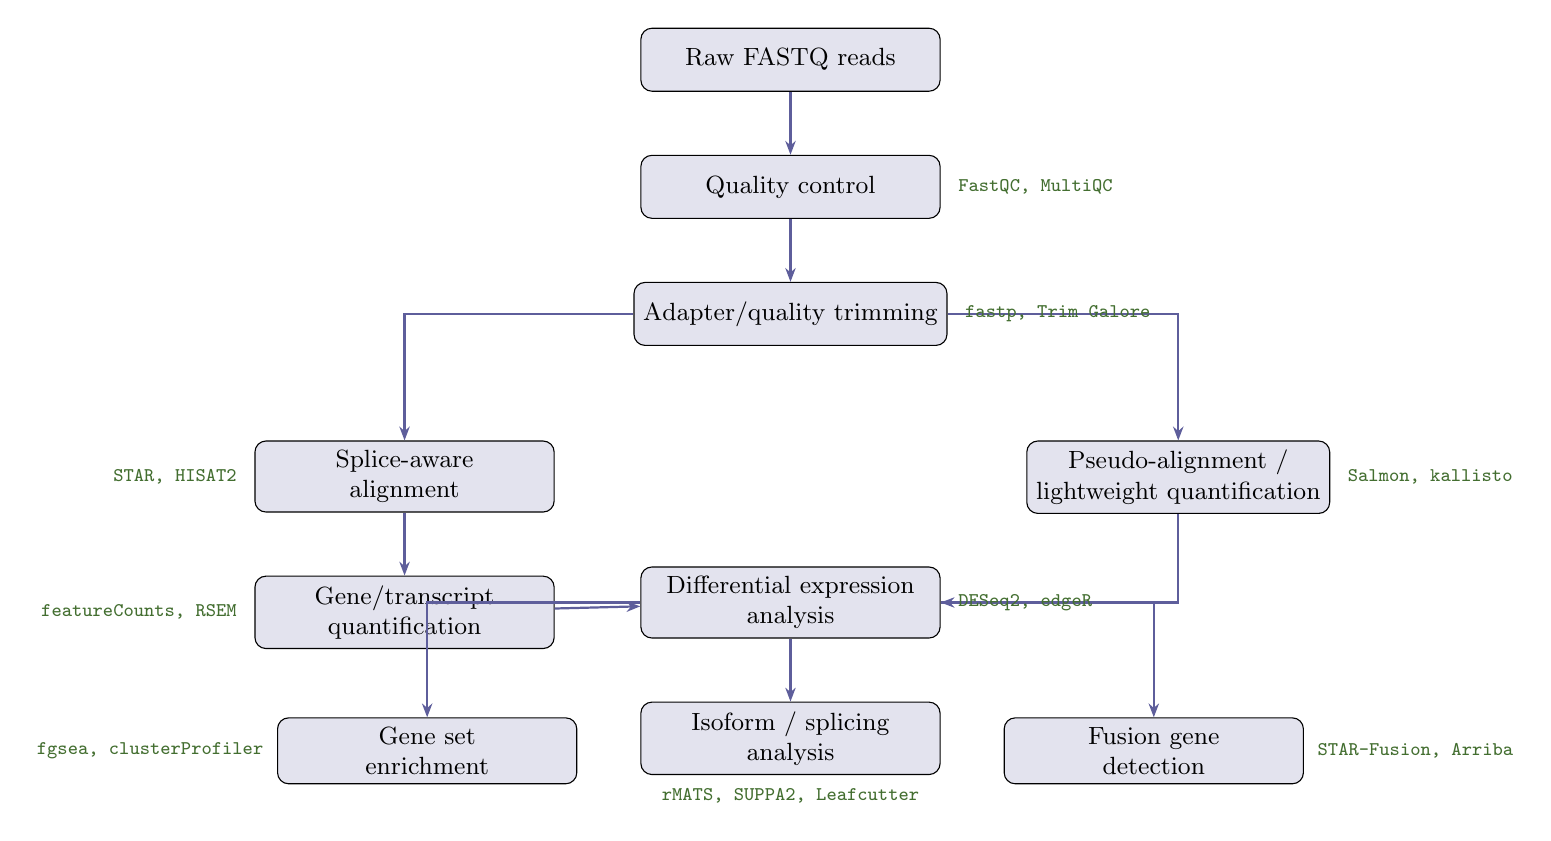
\begin{tikzpicture}[
  node distance=0.8cm and 1.5cm,
  every node/.style={font=\small},
  boxstep/.style={draw, rounded corners, fill=MidnightBlue!12, minimum width=3.8cm, minimum height=0.8cm, align=center, font=\small},
  tool/.style={font=\scriptsize\ttfamily, text=OliveGreen!80!black},
  arrow/.style={-{Stealth[length=5pt]}, thick, MidnightBlue!70},
  branch/.style={-{Stealth[length=5pt]}, thick, BrickRed!70},
]

% Main workflow
\node[boxstep] (raw) {Raw FASTQ reads};
\node[boxstep, below=of raw] (qc) {Quality control};
\node[boxstep, below=of qc] (trim) {Adapter/quality trimming};

% Branch point
\node[boxstep, below left=1.2cm and 1.0cm of trim] (align) {Splice-aware\\alignment};
\node[boxstep, below right=1.2cm and 1.0cm of trim] (pseudo) {Pseudo-alignment /\\lightweight quantification};

% After alignment
\node[boxstep, below=of align] (count) {Gene/transcript\\quantification};

% Merge
\node[boxstep, below=2.8cm of trim] (de) {Differential expression\\analysis};

% Downstream
\node[boxstep, below left=1.0cm and 0.8cm of de] (gsea) {Gene set\\enrichment};
\node[boxstep, below=of de] (iso) {Isoform / splicing\\analysis};
\node[boxstep, below right=1.0cm and 0.8cm of de] (fusion) {Fusion gene\\detection};

% Arrows
\draw[arrow] (raw) -- (qc);
\draw[arrow] (qc) -- (trim);
\draw[arrow] (trim) -| (align);
\draw[arrow] (trim) -| (pseudo);
\draw[arrow] (align) -- (count);
\draw[arrow] (count) -- (de);
\draw[arrow] (pseudo) |- (de);
\draw[arrow] (de) -| (gsea);
\draw[arrow] (de) -- (iso);
\draw[arrow] (de) -| (fusion);

% Tool labels
\node[tool, right=0.1cm of qc] {FastQC, MultiQC};
\node[tool, right=0.1cm of trim] {fastp, Trim Galore};
\node[tool, left=0.1cm of align] {STAR, HISAT2};
\node[tool, right=0.1cm of pseudo] {Salmon, kallisto};
\node[tool, left=0.1cm of count] {featureCounts, RSEM};
\node[tool, right=0.1cm of de] {DESeq2, edgeR};
\node[tool, left=0.05cm of gsea] {fgsea, clusterProfiler};
\node[tool, right=0.05cm of fusion] {STAR-Fusion, Arriba};
\node[tool, below=0.05cm of iso] {rMATS, SUPPA2, Leafcutter};

\end{tikzpicture}
\caption{Overview of the bulk RNA-seq bioinformatics workflow. Two main paths
exist after trimming: alignment-based quantification (left, using STAR/HISAT2
followed by featureCounts) or pseudo-alignment-based quantification (right,
using Salmon/kallisto). Both converge at differential expression analysis.}
\label{fig:rnaseq:workflow}
\end{figure}

\subsection{Quality Control}

\begin{description}[style=nextline]
  \item[\software{FastQC}] Generates per-read-base quality scores, GC content
    distribution, adapter contamination levels, sequence duplication levels,
    and overrepresented sequences for each FASTQ file.
  \item[\software{MultiQC}] Aggregates FastQC (and other tool) reports across
    all samples into a single interactive HTML report. Essential for spotting
    batch effects and outlier samples.
\end{description}

\textbf{Key RNA-seq QC metrics} to monitor:
\begin{itemize}[nosep]
  \item Per-base sequence quality (Phred $\geq$ 30 across the read).
  \item GC content distribution (should match species expectation; bimodal
    distribution suggests contamination).
  \item Adapter content (should be minimal for RNA-seq with appropriate insert
    sizes).
  \item Duplication rate (high duplication may indicate low-complexity library
    or over-amplification).
  \item After alignment: percentage of uniquely mapped reads, percentage of
    reads in exons vs. introns vs. intergenic regions, 5$'$-to-3$'$ gene body
    coverage (detects RNA degradation bias).
\end{itemize}

\subsection{Trimming}

\begin{description}[style=nextline]
  \item[\software{fastp}] All-in-one tool for adapter trimming, quality
    trimming, polyG tail removal (common on NovaSeq two-color chemistry),
    and QC report generation. Fast (multi-threaded C++).
  \item[\software{Trim Galore}] Wrapper around \software{Cutadapt} with
    automatic adapter detection and optional FastQC integration. Widely used in
    RNA-seq pipelines.
\end{description}

\begin{tipbox}
For modern Illumina data, \software{fastp} is often sufficient as the sole
preprocessing step. It performs adapter trimming, quality trimming, and
generates a QC report in a single pass, simplifying the workflow.
\end{tipbox}

\subsection{Alignment: Splice-Aware Aligners}

RNA-seq reads frequently span exon--exon junctions. Standard DNA aligners like
BWA cannot handle these split reads because they expect contiguous alignment
to the reference.

\begin{warningbox}
Never use \software{BWA} or \software{Bowtie2} (DNA aligners) for RNA-seq
read alignment. These tools are not splice-aware and will discard or misalign
reads that span exon--exon junctions, which can constitute 20--40\% of all
reads.
\end{warningbox}

\begin{description}[style=nextline]
  \item[\software{STAR} (Spliced Transcripts Alignment to a Reference)]
    The most widely used RNA-seq aligner. Uses a suffix array-based algorithm
    that is extremely fast but memory-intensive ($\sim$30--40\,GB RAM for
    human genome). Features:
    \begin{itemize}[nosep]
      \item Two-pass mode for improved novel junction detection.
      \item Built-in gene quantification (\texttt{--quantMode GeneCounts}).
      \item Chimeric read detection for fusion gene calling.
      \item \software{STARsolo} mode for single-cell RNA-seq (see \cref{ch:scrnaseq}).
    \end{itemize}
  \item[\software{HISAT2} (Hierarchical Indexing for Spliced Alignment of Transcripts)]
    Uses a graph-based FM index that is much more memory-efficient ($\sim$8\,GB
    for human). Slightly slower than STAR but suitable for machines with limited
    RAM. Successor to TopHat2/Bowtie2.
\end{description}

\subsection{Pseudo-Alignment and Lightweight Quantification}

An alternative to alignment-based approaches, pseudo-alignment (also called
quasi-mapping or lightweight alignment) estimates transcript abundance without
producing a traditional BAM file:

\begin{description}[style=nextline]
  \item[\software{Salmon}] Maps reads to the transcriptome (not genome) using
    selective alignment or quasi-mapping. Corrects for GC bias, sequence-specific
    bias, and fragment length distribution. Outputs transcript-level
    quantification (TPM and estimated counts). Run time: minutes rather than
    hours.
  \item[\software{kallisto}] Uses pseudo-alignment based on k-mer hashing.
    Produces transcript-level abundance estimates. Very fast and
    memory-efficient.
\end{description}

\begin{keyconcept}[title={Alignment vs. Pseudo-Alignment}]
\textbf{Alignment-based} (STAR $\rightarrow$ featureCounts): Produces BAM files
useful for visualization, variant calling, and splicing analysis. Required when
you need genome-level information. \textbf{Pseudo-alignment} (Salmon/kallisto):
Faster, produces transcript-level quantification directly. Excellent for
differential expression and isoform quantification. No BAM file for
visualization. For most differential expression analyses, both approaches yield
highly concordant results.
\end{keyconcept}

\subsection{Gene and Transcript Quantification}

\begin{description}[style=nextline]
  \item[\software{featureCounts} (Subread package)] Assigns aligned reads (from
    BAM files) to genomic features (genes, exons) based on a GTF/GFF
    annotation. Fast and simple. Produces a gene-by-sample count matrix.
    Handles paired-end reads, multi-mapping reads, and strand-specific
    assignments.
  \item[\software{RSEM}] Reference-free estimation of transcript-level
    expression using an expectation-maximization (EM) algorithm. Often used with
    STAR alignment (\texttt{STAR --quantMode TranscriptomeSAM}).
  \item[\software{StringTie}] Assembles transcripts from aligned reads and
    estimates abundance. Particularly useful for novel transcript discovery and
    isoform-level quantification.
\end{description}

\subsection{Differential Expression Analysis}

Differential expression (DE) analysis identifies genes whose expression differs
significantly between experimental conditions. The three dominant tools all use
negative binomial generalized linear models:

\begin{description}[style=nextline]
  \item[\software{DESeq2} (R/Bioconductor)] Uses shrinkage estimation for
    dispersion and fold changes. Provides independent filtering and Benjamini--Hochberg
    adjusted $p$-values. The most cited DE tool. Recommended for studies with
    $\geq$ 3 replicates per condition.
  \item[\software{edgeR} (R/Bioconductor)] Uses empirical Bayes methods for
    dispersion estimation. Slightly more liberal than DESeq2 in some benchmarks.
    Offers both exact tests and GLM-based approaches (quasi-likelihood F-tests
    are recommended for complex designs).
  \item[\software{limma-voom} (R/Bioconductor)] Transforms count data using the
    voom method (variance modeling at the observational level) and applies the
    limma linear modeling framework. Particularly powerful for complex
    experimental designs with multiple factors and interactions. Often performs
    well with larger sample sizes ($n > 10$ per group).
\end{description}

\begin{tipbox}
When importing Salmon or kallisto transcript-level counts into R, use the
\software{tximport} or \software{tximeta} package. These tools correctly
aggregate transcript-level estimates to gene-level counts while accounting for
changes in transcript length across samples---a bias that simple summing ignores.
\end{tipbox}

\subsection{The Negative Binomial Distribution for RNA-seq}
\label{subsec:rnaseq:negbinom}

RNA-seq read counts are \emph{discrete} non-negative integers, making continuous
distributions like the normal distribution inappropriate. A natural first model
is the Poisson distribution, where the variance equals the mean:
$\text{Var}(Y) = \mu$. However, biological replicates exhibit
\textbf{overdispersion}---the observed variance exceeds the Poisson expectation
because biological samples differ from one another beyond what sampling noise
alone would predict. A gene with mean expression $\mu = 100$ across replicates
may have variance of 500 or more, far larger than the Poisson prediction of 100.

The \textbf{negative binomial (NB) distribution} accounts for this
overdispersion by introducing a dispersion parameter $\alpha$ (also written
$\phi$ or $1/r$ in different parameterizations):
\begin{equation}
  \label{eq:rnaseq:nbvar}
  \text{Var}(Y) = \mu + \alpha\mu^2
\end{equation}
where $\mu$ is the mean expression and $\alpha \geq 0$ is the gene-specific
dispersion. When $\alpha = 0$, the NB reduces to the Poisson. For most genes in
a typical RNA-seq experiment, $\alpha$ ranges from 0.01 to 0.5. The probability
mass function of the NB distribution (using the mean-dispersion
parameterization) is:
\begin{equation}
  \label{eq:rnaseq:nbpmf}
  P(Y = k) = \binom{k + r - 1}{k}
    \left(\frac{r}{r + \mu}\right)^{r}
    \left(\frac{\mu}{r + \mu}\right)^{k},
    \qquad r = \frac{1}{\alpha}
\end{equation}
where $r = 1/\alpha$ is the size (or inverse dispersion) parameter.

\begin{keyconcept}[title={Why Not Poisson?}]
The Poisson model underestimates variance in RNA-seq data because it cannot
represent biological variability between replicates. Using a Poisson test
(e.g., an exact Poisson test in early RNA-seq tools) produces dramatically
inflated false-positive rates. All modern DE tools---\software{DESeq2},
\software{edgeR}, and \software{limma-voom}---use models that accommodate
overdispersion: the negative binomial GLM (\software{DESeq2}, \software{edgeR})
or variance-weighted linear models (\software{limma-voom}).
\end{keyconcept}

\subsection{DESeq2 Dispersion Estimation and Shrinkage}
\label{subsec:rnaseq:deseq2dispersion}

Accurate estimation of the gene-specific dispersion $\alpha_i$ is the central
statistical challenge in RNA-seq differential expression. With only 3--6
replicates per condition, per-gene maximum-likelihood estimates of $\alpha_i$
are highly noisy. \software{DESeq2} addresses this through a three-step
\textbf{dispersion shrinkage} procedure:

\begin{enumerate}[nosep]
  \item \textbf{Gene-wise dispersion estimates.} For each gene $i$,
    \software{DESeq2} computes a maximum-likelihood estimate $\hat{\alpha}_i^{\text{MLE}}$
    by fitting a negative binomial GLM using the Cox--Reid adjusted profile
    likelihood. These estimates are highly variable when the number of replicates
    is small.
  \item \textbf{Fitted dispersion trend.} A smooth function
    $\alpha_{\text{tr}}(\mu)$ is fitted to the gene-wise estimates as a function
    of the mean expression $\mu_i$. This trend captures the systematic
    relationship between dispersion and expression level (lowly expressed genes
    tend to have higher dispersion). The parametric fit is typically of the form:
    \begin{equation}
      \label{eq:rnaseq:disptrend}
      \alpha_{\text{tr}}(\mu) = \frac{a_1}{\mu} + a_0
    \end{equation}
    where $a_0$ and $a_1$ are estimated by regression.
  \item \textbf{Shrinkage toward the trend.} Each gene-wise estimate is
    shrunk toward the trend using a log-normal prior centered on
    $\log(\alpha_{\text{tr}}(\mu_i))$. The final maximum a posteriori (MAP)
    estimate balances the gene-specific data with the global trend:
    \begin{equation}
      \label{eq:rnaseq:dispmap}
      \hat{\alpha}_i^{\text{MAP}} = \arg\max_{\alpha_i}
        \left[
          \ell(\alpha_i \mid Y_i) +
          \log \pi(\alpha_i \mid \alpha_{\text{tr}}(\mu_i), \sigma_d^2)
        \right]
    \end{equation}
    where $\ell$ is the log-likelihood and $\pi$ is the log-normal prior with
    variance $\sigma_d^2$ estimated from the data. Genes with very high
    dispersion (outliers above the trend) are not shrunk, to avoid
    underestimating their variance and inflating false positives.
\end{enumerate}

\begin{tipbox}
The \software{edgeR} package uses a conceptually similar but technically
different approach. It estimates a common dispersion across all genes and
gene-wise dispersions, then shrinks gene-wise estimates toward the common
(or trended) dispersion using a weighted likelihood empirical Bayes procedure.
The key difference is that \software{edgeR} uses a weighted likelihood approach
rather than a prior distribution, and its quasi-likelihood F-test (recommended
for complex designs) adds a second layer of overdispersion modeling.
\end{tipbox}

\subsection{Normalisation Methods for RNA-seq}
\label{subsec:rnaseq:normalisation}

Raw read counts cannot be compared directly across genes or samples because they
are confounded by gene length, library size (total sequencing depth), and RNA
composition. Several normalisation metrics address different subsets of these
biases:

\begin{description}[style=nextline]
  \item[RPKM (Reads Per Kilobase per Million mapped reads)]
    Normalises for both gene length and sequencing depth. Used for single-end
    data:
    \begin{equation}
      \label{eq:rnaseq:rpkm}
      \text{RPKM}_i = \frac{c_i \times 10^9}{N \times l_i}
    \end{equation}
    where $c_i$ is the raw count for gene $i$, $N$ is the total number of mapped
    reads in the sample, and $l_i$ is the effective gene length in base pairs.
  \item[FPKM (Fragments Per Kilobase per Million mapped fragments)]
    The paired-end equivalent of RPKM, where $N$ counts fragments (read pairs)
    rather than individual reads. The formula is identical to RPKM but uses
    fragment counts, avoiding double-counting of paired-end reads.
  \item[TPM (Transcripts Per Million)]
    A two-step normalisation that first divides by gene length, then normalises
    to a fixed sum:
    \begin{equation}
      \label{eq:rnaseq:tpm}
      \text{TPM}_i = \frac{c_i / l_i}{\sum_{j} (c_j / l_j)} \times 10^6
    \end{equation}
    Because TPM values within each sample sum to exactly $10^6$, the relative
    proportions are directly comparable across samples---a property that RPKM/FPKM
    lack (their column sums vary with the gene length distribution of expressed
    genes).
\end{description}

\begin{warningbox}
RPKM and FPKM values are \textbf{not directly comparable across samples}
because the denominator $N$ includes all mapped reads, and the gene-length
normalisation step alters the effective library size differently depending on
which genes are expressed in each sample. TPM resolves this by normalising to a
fixed sum. For this reason, TPM has largely replaced RPKM/FPKM in modern
publications. However, for differential expression analysis, none of these
within-sample metrics are appropriate---use the raw counts with \software{DESeq2}
or \software{edgeR}, which apply their own between-sample normalisation
(median-of-ratios or TMM, respectively).
\end{warningbox}

\begin{keyconcept}[title={DESeq2 Median-of-Ratios Normalisation}]
\software{DESeq2} computes a \emph{size factor} $s_j$ for each sample $j$ as
the median of the ratios of observed counts to the geometric mean across
samples:
\begin{equation}
  \label{eq:rnaseq:sizefactor}
  s_j = \text{median}_i \frac{c_{ij}}{\left(\prod_{j'=1}^{m} c_{ij'}\right)^{1/m}}
\end{equation}
This approach is robust to highly expressed genes that dominate a few samples
and accounts for RNA composition differences---a major advantage over simple
library-size normalisation.
\end{keyconcept}

\subsection{DESeq2 vs.\ edgeR vs.\ limma-voom: A Detailed Comparison}
\label{subsec:rnaseq:detools_comparison}

\begin{table}[htbp]
\centering
\caption{Detailed comparison of the three major differential expression tools
for bulk RNA-seq.}
\label{tab:rnaseq:de_comparison}
\small
\begin{tabularx}{\textwidth}{lXXX}
\toprule
\textbf{Feature} & \textbf{DESeq2} & \textbf{edgeR} & \textbf{limma-voom} \\
\midrule
Statistical model & Negative binomial GLM & Negative binomial GLM (QL F-test recommended) & Weighted linear model on log-CPM \\
Normalisation & Median-of-ratios (size factors) & Trimmed mean of M-values (TMM) & TMM (via edgeR) or quantile \\
Dispersion estimation & Gene-wise MLE $\rightarrow$ trend $\rightarrow$ MAP shrinkage (log-normal prior) & Gene-wise $\rightarrow$ trended $\rightarrow$ empirical Bayes squeeze (weighted likelihood) & Mean-variance trend modeled by voom; precision weights per observation \\
Shrinkage of fold changes & Optional (apeglm, ashr, normal) & No built-in LFC shrinkage & Empirical Bayes moderation of $t$-statistics \\
Multiple testing & Benjamini--Hochberg with independent filtering & Benjamini--Hochberg & Benjamini--Hochberg \\
Complex designs & Supported (interaction terms, continuous covariates) & Excellent (quasi-likelihood framework is very flexible) & Excellent (full linear model framework; best for large, complex designs) \\
Speed (20k genes, $n$=20) & $\sim$1--3 minutes & $\sim$30 seconds--1 minute & $\sim$10--30 seconds \\
Best for & Standard two-group comparisons with small $n$; strong defaults & Complex experimental designs; large datasets & Very large sample sizes ($n > 20$); complex multi-factor designs \\
\bottomrule
\end{tabularx}
\end{table}

\begin{tipbox}
In practice, all three tools produce highly overlapping results for well-designed
experiments with adequate replication. \software{DESeq2} is the most popular due
to its sensible defaults and extensive documentation. \software{edgeR} with
quasi-likelihood F-tests is preferred for complex designs with multiple factors.
\software{limma-voom} excels when sample sizes are large (e.g., GTEx-scale
studies with hundreds of samples) because its linear model framework is both
fast and statistically powerful. For the most robust results, consider running
two tools and focusing on the intersection of significant genes.
\end{tipbox}

\subsection{Gene Set Enrichment Analysis}

After identifying differentially expressed genes, the next step is biological
interpretation:

\begin{description}[style=nextline]
  \item[\software{GSEA} (Gene Set Enrichment Analysis)] The original
    Broad Institute tool. Uses a ranked list of all genes (not just significant
    ones) to determine whether predefined gene sets (e.g., GO terms, KEGG
    pathways, MSigDB collections) are enriched at the top or bottom of the
    ranking. Avoids the arbitrary cutoff problem of over-representation analysis.
  \item[\software{fgsea} (R/Bioconductor)] Fast implementation of the GSEA
    algorithm in R. Orders of magnitude faster than the original Java tool.
  \item[\software{clusterProfiler} (R/Bioconductor)] Comprehensive enrichment
    analysis package supporting Gene Ontology (GO), KEGG, Reactome, Disease
    Ontology, and custom gene sets. Performs both over-representation analysis
    (ORA) and GSEA. Provides publication-quality visualization functions
    (dot plots, enrichment maps, ridge plots).
  \item[\software{enrichR}] Web-based tool with an R API that queries $>$200
    gene set libraries including ENCODE, ChEA, and other curated databases.
\end{description}

\subsection{Isoform and Splicing Analysis}

\begin{description}[style=nextline]
  \item[\software{rMATS} (replicate Multivariate Analysis of Transcript Splicing)]
    Detects differential alternative splicing events from RNA-seq data.
    Classifies events into five types: skipped exon (SE), retained intron
    (RI), mutually exclusive exons (MXE), alternative 5$'$ splice site (A5SS),
    and alternative 3$'$ splice site (A3SS). Uses a Bayesian framework to
    estimate inclusion levels ($\Psi$ / PSI values) and their differences.
  \item[\software{SUPPA2}] Fast differential splicing analysis using percent
    spliced-in (PSI) values calculated directly from transcript quantification
    (Salmon/kallisto output). Does not require BAM files.
  \item[\software{Leafcutter}] Detects differential intron usage without
    requiring transcript annotations. Identifies intron excision clusters and
    tests for differential usage between conditions. Annotation-free approach
    is particularly valuable for non-model organisms.
\end{description}

\subsection{Fusion Gene Detection}

Gene fusions---where two normally separate genes are joined---are hallmarks of
many cancers (e.g., \gene{BCR-ABL1} in CML, \gene{EML4-ALK} in lung cancer).

\begin{description}[style=nextline]
  \item[\software{STAR-Fusion}] Uses chimeric read alignments from STAR to
    detect fusion transcripts. Integrates with the FusionInspector
    visualization tool and with CTAT (Cancer Transcriptome Analysis Toolkit).
  \item[\software{Arriba}] Fast and accurate fusion detection from STAR chimeric
    alignments. Known for low false-positive rate and built-in visualization
    of fusion events with gene structure diagrams.
\end{description}


% ---------------------------------------------------------------------------
\section{Complete Snakemake Workflow for RNA-seq}
\label{sec:rnaseq:snakemake}

\begin{lstlisting}[language=Python, caption={Complete Snakemake workflow for
bulk RNA-seq analysis with STAR alignment and featureCounts quantification.},
label={lst:rnaseq:snakemake}, float=htbp]
# Snakefile for Bulk RNA-seq Analysis
# ====================================
# Pipeline: FastQC -> fastp -> STAR -> featureCounts -> DESeq2

import pandas as pd

configfile: "config/config.yaml"

# Load sample sheet
samples = pd.read_csv(config["samples"], sep="\t")
SAMPLES = samples["sample"].tolist()

# Reference files
GENOME_DIR = config["star_index"]
GTF = config["gtf"]
FASTA = config["genome_fasta"]

rule all:
    input:
        "results/multiqc/multiqc_report.html",
        "results/counts/gene_counts.tsv",
        "results/deseq2/differential_expression.csv",
        expand("results/fastqc_raw/{sample}_{read}_fastqc.html",
               sample=SAMPLES, read=["R1", "R2"]),
        expand("results/bigwig/{sample}.bw", sample=SAMPLES)

rule fastqc_raw:
    input:
        "data/raw/{sample}_{read}.fastq.gz"
    output:
        html="results/fastqc_raw/{sample}_{read}_fastqc.html",
        zip="results/fastqc_raw/{sample}_{read}_fastqc.zip"
    threads: 2
    conda: "envs/qc.yaml"
    shell:
        "fastqc -t {threads} -o results/fastqc_raw/ {input}"

rule fastp:
    input:
        r1="data/raw/{sample}_R1.fastq.gz",
        r2="data/raw/{sample}_R2.fastq.gz"
    output:
        r1="results/trimmed/{sample}_R1.fastq.gz",
        r2="results/trimmed/{sample}_R2.fastq.gz",
        html="results/fastp/{sample}.html",
        json="results/fastp/{sample}.json"
    threads: 4
    conda: "envs/qc.yaml"
    shell:
        """
        fastp \
          --in1 {input.r1} --in2 {input.r2} \
          --out1 {output.r1} --out2 {output.r2} \
          --html {output.html} --json {output.json} \
          --detect_adapter_for_pe \
          --qualified_quality_phred 20 \
          --length_required 35 \
          --thread {threads}
        """

rule star_index:
    input:
        fasta=FASTA,
        gtf=GTF
    output:
        directory("resources/star_index")
    threads: 12
    resources:
        mem_mb=40000
    conda: "envs/align.yaml"
    shell:
        """
        STAR --runMode genomeGenerate \
          --genomeDir {output} \
          --genomeFastaFiles {input.fasta} \
          --sjdbGTFfile {input.gtf} \
          --sjdbOverhang 149 \
          --runThreadN {threads}
        """

rule star_align:
    input:
        r1="results/trimmed/{sample}_R1.fastq.gz",
        r2="results/trimmed/{sample}_R2.fastq.gz",
        index=GENOME_DIR
    output:
        bam="results/star/{sample}/Aligned.sortedByCoord.out.bam",
        log="results/star/{sample}/Log.final.out",
        sj="results/star/{sample}/SJ.out.tab"
    threads: 8
    resources:
        mem_mb=36000
    params:
        prefix="results/star/{sample}/"
    conda: "envs/align.yaml"
    shell:
        """
        STAR --runMode alignReads \
          --genomeDir {input.index} \
          --readFilesIn {input.r1} {input.r2} \
          --readFilesCommand zcat \
          --outSAMtype BAM SortedByCoordinate \
          --outSAMstrandField intronMotif \
          --quantMode GeneCounts \
          --twopassMode Basic \
          --outFileNamePrefix {params.prefix} \
          --runThreadN {threads} \
          --outSAMattributes NH HI AS NM MD \
          --outFilterMultimapNmax 20 \
          --alignSJoverhangMin 8 \
          --alignSJDBoverhangMin 1 \
          --chimSegmentMin 20 \
          --chimJunctionOverhangMin 20
        """

rule index_bam:
    input:
        "results/star/{sample}/Aligned.sortedByCoord.out.bam"
    output:
        "results/star/{sample}/Aligned.sortedByCoord.out.bam.bai"
    conda: "envs/align.yaml"
    shell:
        "samtools index {input}"

rule featurecounts:
    input:
        bams=expand(
            "results/star/{sample}/Aligned.sortedByCoord.out.bam",
            sample=SAMPLES),
        gtf=GTF
    output:
        counts="results/counts/gene_counts.tsv",
        summary="results/counts/gene_counts.tsv.summary"
    threads: 4
    params:
        strandedness=2  # 2 = reverse-stranded (dUTP)
    conda: "envs/quantify.yaml"
    shell:
        """
        featureCounts \
          -a {input.gtf} \
          -o {output.counts} \
          -p --countReadPairs \
          -s {params.strandedness} \
          -T {threads} \
          -B -C \
          --extraAttributes gene_name \
          {input.bams}
        """

rule bigwig:
    input:
        bam="results/star/{sample}/Aligned.sortedByCoord.out.bam",
        bai="results/star/{sample}/Aligned.sortedByCoord.out.bam.bai"
    output:
        "results/bigwig/{sample}.bw"
    threads: 4
    conda: "envs/quantify.yaml"
    shell:
        """
        bamCoverage -b {input.bam} -o {output} \
          --normalizeUsing RPKM \
          --binSize 10 \
          -p {threads}
        """

rule multiqc:
    input:
        expand("results/fastqc_raw/{sample}_{read}_fastqc.zip",
               sample=SAMPLES, read=["R1", "R2"]),
        expand("results/fastp/{sample}.json", sample=SAMPLES),
        expand("results/star/{sample}/Log.final.out",
               sample=SAMPLES),
        "results/counts/gene_counts.tsv.summary"
    output:
        "results/multiqc/multiqc_report.html"
    conda: "envs/qc.yaml"
    shell:
        "multiqc results/ -o results/multiqc/ --force"

rule deseq2:
    input:
        counts="results/counts/gene_counts.tsv",
        samples=config["samples"]
    output:
        results="results/deseq2/differential_expression.csv",
        ma_plot="results/deseq2/ma_plot.pdf",
        volcano="results/deseq2/volcano_plot.pdf",
        pca="results/deseq2/pca_plot.pdf"
    conda: "envs/deseq2.yaml"
    script:
        "scripts/run_deseq2.R"
\end{lstlisting}


% ---------------------------------------------------------------------------
\section{Complete Nextflow Workflow for RNA-seq}
\label{sec:rnaseq:nextflow}

\begin{lstlisting}[language=Java, caption={Complete Nextflow DSL2 workflow for
bulk RNA-seq analysis with STAR alignment and featureCounts quantification.},
label={lst:rnaseq:nextflow}, float=htbp]
#!/usr/bin/env nextflow
// RNA-seq Analysis Pipeline (Nextflow DSL2)
// ==========================================
// Pipeline: FastQC -> fastp -> STAR -> featureCounts -> DESeq2

nextflow.enable.dsl = 2

params.reads       = "data/raw/*_{R1,R2}.fastq.gz"
params.genome      = "resources/genome.fa"
params.gtf         = "resources/genes.gtf"
params.star_index  = null
params.outdir      = "results"
params.strandedness = 2  // 2 = reverse-stranded (dUTP)

// Print pipeline info
log.info """
=============================
 RNA-seq Analysis Pipeline
=============================
 reads        : ${params.reads}
 genome       : ${params.genome}
 GTF          : ${params.gtf}
 strandedness : ${params.strandedness}
 outdir       : ${params.outdir}
=============================
"""

// --- Processes ---

process FASTQC {
    tag "$sample_id"
    publishDir "${params.outdir}/fastqc", mode: 'copy'
    cpus 2

    input:
    tuple val(sample_id), path(reads)

    output:
    path("*.html"), emit: html
    path("*.zip"),  emit: zip

    script:
    """
    fastqc -t ${task.cpus} ${reads}
    """
}

process FASTP {
    tag "$sample_id"
    publishDir "${params.outdir}/fastp", mode: 'copy'
    cpus 4

    input:
    tuple val(sample_id), path(reads)

    output:
    tuple val(sample_id), path("*_trimmed_R{1,2}.fastq.gz"),
        emit: trimmed_reads
    path("*.html"), emit: html
    path("*.json"), emit: json

    script:
    def (r1, r2) = reads
    """
    fastp \
      --in1 ${r1} --in2 ${r2} \
      --out1 ${sample_id}_trimmed_R1.fastq.gz \
      --out2 ${sample_id}_trimmed_R2.fastq.gz \
      --html ${sample_id}_fastp.html \
      --json ${sample_id}_fastp.json \
      --detect_adapter_for_pe \
      --qualified_quality_phred 20 \
      --length_required 35 \
      --thread ${task.cpus}
    """
}

process STAR_INDEX {
    publishDir "${params.outdir}/star_index", mode: 'copy'
    cpus 12
    memory '40 GB'

    input:
    path(genome)
    path(gtf)

    output:
    path("star_index"), emit: index

    script:
    """
    mkdir -p star_index
    STAR --runMode genomeGenerate \
      --genomeDir star_index \
      --genomeFastaFiles ${genome} \
      --sjdbGTFfile ${gtf} \
      --sjdbOverhang 149 \
      --runThreadN ${task.cpus}
    """
}

process STAR_ALIGN {
    tag "$sample_id"
    publishDir "${params.outdir}/star/${sample_id}", mode: 'copy'
    cpus 8
    memory '36 GB'

    input:
    tuple val(sample_id), path(reads)
    path(index)

    output:
    tuple val(sample_id),
        path("*Aligned.sortedByCoord.out.bam"), emit: bam
    path("*Log.final.out"),                     emit: log
    path("*SJ.out.tab"),                        emit: sj

    script:
    def (r1, r2) = reads
    """
    STAR --runMode alignReads \
      --genomeDir ${index} \
      --readFilesIn ${r1} ${r2} \
      --readFilesCommand zcat \
      --outSAMtype BAM SortedByCoordinate \
      --outSAMstrandField intronMotif \
      --quantMode GeneCounts \
      --twopassMode Basic \
      --outFileNamePrefix ${sample_id}_ \
      --runThreadN ${task.cpus} \
      --outSAMattributes NH HI AS NM MD \
      --outFilterMultimapNmax 20 \
      --chimSegmentMin 20
    """
}

process FEATURECOUNTS {
    publishDir "${params.outdir}/counts", mode: 'copy'
    cpus 4

    input:
    path(bams)
    path(gtf)

    output:
    path("gene_counts.tsv"),         emit: counts
    path("gene_counts.tsv.summary"), emit: summary

    script:
    """
    featureCounts \
      -a ${gtf} \
      -o gene_counts.tsv \
      -p --countReadPairs \
      -s ${params.strandedness} \
      -T ${task.cpus} \
      -B -C \
      ${bams}
    """
}

process MULTIQC {
    publishDir "${params.outdir}/multiqc", mode: 'copy'

    input:
    path('*')

    output:
    path("multiqc_report.html")

    script:
    """
    multiqc . -o . --force
    """
}

process DESEQ2 {
    publishDir "${params.outdir}/deseq2", mode: 'copy'

    input:
    path(counts)
    path(sample_sheet)

    output:
    path("differential_expression.csv"), emit: results
    path("*.pdf"), emit: plots

    script:
    """
    Rscript ${projectDir}/bin/run_deseq2.R \
      --counts ${counts} \
      --samples ${sample_sheet} \
      --outdir .
    """
}

// --- Workflow ---

workflow {
    // Create channel from read pairs
    reads_ch = Channel
        .fromFilePairs(params.reads, checkIfExists: true)

    // Quality control on raw reads
    FASTQC(reads_ch)

    // Adapter and quality trimming
    FASTP(reads_ch)

    // Build STAR index if not provided
    if (params.star_index) {
        star_index = Channel.fromPath(params.star_index)
    } else {
        STAR_INDEX(
            Channel.fromPath(params.genome),
            Channel.fromPath(params.gtf)
        )
        star_index = STAR_INDEX.out.index
    }

    // Align reads with STAR
    STAR_ALIGN(FASTP.out.trimmed_reads, star_index.collect())

    // Quantify with featureCounts
    FEATURECOUNTS(
        STAR_ALIGN.out.bam.map { it[1] }.collect(),
        Channel.fromPath(params.gtf)
    )

    // Aggregate QC reports
    MULTIQC(
        FASTQC.out.zip
            .mix(FASTP.out.json)
            .mix(STAR_ALIGN.out.log)
            .mix(FEATURECOUNTS.out.summary)
            .collect()
    )
}
\end{lstlisting}

\begin{tipbox}
For production use, consider the \software{nf-core/rnaseq} pipeline, which
implements a full-featured, peer-reviewed RNA-seq workflow in Nextflow with
extensive QC, multiple aligner/quantifier options, and compatibility with
institutional HPC systems and cloud environments. As of v3.14, it supports
STAR, HISAT2, Salmon, and RSEM, with automatic strandedness detection.
\end{tipbox}


% ---------------------------------------------------------------------------
\section{Experimental Design for RNA-seq}
\label{sec:rnaseq:design}

\subsection{Biological Replicates}

\begin{keyconcept}[title={Replication is Non-Negotiable}]
Biological replicates are essential for statistical inference. Technical
replicates (sequencing the same library twice) do not capture biological
variability and are rarely needed given the high reproducibility of modern
sequencing. The minimum is \textbf{3 biological replicates per condition};
\textbf{5--6 replicates} substantially increase power to detect smaller fold
changes. For heterogeneous clinical samples, even more replicates are
advisable.
\end{keyconcept}

Power analysis tools such as \software{RNASeqPower} (R/Bioconductor) and
\software{PROPER} can estimate the number of replicates needed given expected
effect sizes, dispersion, and sequencing depth.

\subsection{Sequencing Depth}

\begin{table}[htbp]
\centering
\caption{Recommended sequencing depths for common RNA-seq applications.}
\label{tab:rnaseq:depth}
\begin{tabularx}{\textwidth}{lXr}
\toprule
\textbf{Application} & \textbf{Rationale} & \textbf{Reads/sample} \\
\midrule
Differential gene expression & Sufficient to quantify $\sim$15,000 expressed genes & 20--30M \\
Isoform-level analysis & Need to distinguish splice variants & 50--100M \\
Novel transcript discovery & Deeper coverage of low-abundance transcripts & 80--150M \\
Small RNA-seq & Smaller library; many reads are adapter dimers & 10--20M \\
Total RNA-seq (rRNA depleted) & Compensate for residual rRNA reads & 40--60M \\
FFPE RNA-seq & Higher duplicate rate reduces usable reads & 50--80M \\
\bottomrule
\end{tabularx}
\end{table}

\begin{tipbox}
In most cases, adding biological replicates provides more statistical power
than increasing sequencing depth beyond 20--30M reads per sample. Budget your
sequencing funds toward more replicates rather than deeper sequencing, unless
you specifically need isoform-level resolution.
\end{tipbox}

\subsection{Batch Effects and Their Mitigation}

Batch effects are systematic technical differences between groups of samples
processed at different times, by different operators, or on different flow
cells. They can be devastating in RNA-seq because they may confound or entirely
obscure biological signal.

\textbf{Prevention (most important):}
\begin{itemize}[nosep]
  \item Extract RNA from all samples in the same session if possible.
  \item Prepare libraries in a single batch.
  \item If batching is unavoidable, \textbf{balance experimental groups across
    batches} (do not process all controls in batch 1 and all treatments in
    batch 2).
  \item Record batch information meticulously.
\end{itemize}

\textbf{Computational correction (second line of defense):}
\begin{description}[style=nextline]
  \item[\software{ComBat} (sva package)] Empirical Bayes framework for batch
    effect adjustment. Operates on normalized expression matrices. Widely used
    and effective but can remove real biological signal if batch and condition
    are confounded.
  \item[\software{limma::removeBatchEffect}] Removes batch effects from a
    normalized expression matrix for visualization purposes (PCA, heatmaps).
    For differential expression, include batch as a covariate in the DE model
    instead.
  \item[Inclusion in the DE model] The statistically preferred approach: add
    batch as a covariate in the DESeq2 or edgeR design formula (e.g.,
    \texttt{\textasciitilde{} batch + condition}). This separates batch
    variance from treatment variance without modifying the data.
\end{description}

\begin{warningbox}
If batch is completely confounded with the biological variable of interest
(e.g., all treatment samples were processed in January and all controls in
March), no computational method can rescue the experiment. The only solution
is to re-design and re-run the experiment with proper balancing.
\end{warningbox}


% ---------------------------------------------------------------------------
\section{RNA-seq Approaches: Comprehensive Comparison}
\label{sec:rnaseq:comparison}

\begin{table}[htbp]
\centering
\caption{Comprehensive comparison of RNA-seq approaches.}
\label{tab:rnaseq:approaches}
\small
\begin{tabularx}{\textwidth}{lXXXX}
\toprule
\textbf{Feature} & \textbf{mRNA-seq} & \textbf{Total RNA-seq} & \textbf{Small RNA-seq} & \textbf{Long-read RNA-seq} \\
\midrule
Target & Poly-A$^+$ mRNA & All RNA (rRNA depleted) & miRNA, piRNA, tRFs & Full-length transcripts \\
Read length & 2$\times$150\,bp & 2$\times$150\,bp & 1$\times$50--75\,bp & 1--20\,kb \\
Platform & Illumina & Illumina & Illumina & PacBio, ONT \\
Input RNA & 100\,ng--1\,$\mu$g & 100\,ng--1\,$\mu$g & 100\,ng--1\,$\mu$g & 300\,ng--5\,$\mu$g \\
Quality req. & RIN $\geq$ 7 & RIN $\geq$ 2 (with rRNA depl.) & RIN $\geq$ 7 & RIN $\geq$ 7 (Iso-Seq) \\
Isoform resolution & Limited & Limited & N/A & Excellent \\
ncRNA coverage & Minimal & Comprehensive & Small ncRNA only & Good \\
Depth needed & 20--30M & 40--60M & 10--20M & 1--10M \\
Cost/sample & \$\$  & \$\$ & \$ & \$\$\$ \\
Main use case & Standard DE & Degraded samples, ncRNA & miRNA profiling & Isoform discovery \\
\bottomrule
\end{tabularx}
\end{table}


% ---------------------------------------------------------------------------
\section{Chapter Summary}
\label{sec:rnaseq:summary}

RNA-seq is the workhorse technology of modern transcriptomics, applicable to
an extraordinary range of biological questions. In this chapter we covered:

\begin{itemize}[nosep]
  \item The rationale for measuring RNA and the complexity of the transcriptome.
  \item Poly-A selection (mRNA-seq) versus ribosomal depletion (total RNA-seq)
    and when to use each.
  \item Library preparation details: strand-specific protocols (dUTP method),
    low-input protocols (Smart-seq), and degraded RNA handling (FFPE).
  \item Small RNA sequencing for miRNAs and other small non-coding RNAs.
  \item Long-read RNA-seq (PacBio Iso-Seq, ONT direct RNA) for full-length
    isoform characterization.
  \item Nascent RNA methods (GRO-seq, PRO-seq, NET-seq, TT-seq) for measuring
    active transcription.
  \item The complete bioinformatics pipeline: QC, trimming, alignment (STAR,
    HISAT2), quantification (featureCounts, Salmon), differential expression
    (DESeq2, edgeR, limma-voom), gene set enrichment, isoform analysis, and
    fusion detection.
  \item Practical workflows in both Snakemake and Nextflow.
  \item Experimental design: replication, sequencing depth, and batch effect
    management.
\end{itemize}

In the next chapter, we move from bulk tissue-level measurements to the
resolution of individual cells with single-cell RNA sequencing
(\cref{ch:scrnaseq}).

% ==============================================================================
% Chapter 11: Single-Cell RNA Sequencing
% ==============================================================================
\chapter{Single-Cell RNA Sequencing}
\label{ch:scrnaseq}

\begin{keyconcept}
Single-cell RNA sequencing (\acrshort{scRNA-seq}) measures the transcriptome
of individual cells, revealing cellular heterogeneity that is invisible to bulk
RNA-seq. It has transformed our understanding of development, immunology,
neuroscience, and cancer by enabling the identification of rare cell types,
continuous differentiation trajectories, and cell-state-specific gene
regulatory programs.
\end{keyconcept}

% ---------------------------------------------------------------------------
\section{Why Single-Cell Resolution?}
\label{sec:scrnaseq:why}

\subsection{The Limitation of Bulk RNA-seq}

Bulk RNA-seq measures the \emph{average} gene expression across a population
of $10^5$--$10^7$ cells. This averaging has profound consequences:

\begin{itemize}[nosep]
  \item \textbf{Masking of rare populations:} A cell type comprising 1\% of a
    tissue may be functionally critical (e.g., stem cells, tumor-initiating
    cells) but its transcriptional signature is diluted beyond detection in
    bulk data.
  \item \textbf{False intermediate states:} A mixture of two distinct cell
    states (e.g., activated and resting T cells) appears in bulk as a single
    ``intermediate'' state that does not actually exist in any individual cell.
  \item \textbf{Ecological fallacy:} Correlations observed at the bulk level
    may not hold at the single-cell level. Two genes may appear co-expressed
    in bulk data simply because they are expressed in different subpopulations
    that co-vary in proportion.
  \item \textbf{No trajectory information:} Bulk RNA-seq provides a snapshot
    but cannot reveal the order of events during dynamic processes such as
    differentiation, reprogramming, or drug response.
\end{itemize}

\subsection{What Single-Cell Resolution Enables}

\begin{enumerate}[nosep]
  \item \textbf{Cell type discovery:} Unbiased identification of cell types
    and subtypes without prior marker knowledge.
  \item \textbf{Developmental trajectories:} Reconstruction of differentiation
    paths and branching decisions using pseudotime analysis.
  \item \textbf{Gene regulatory networks:} Inference of transcription factor
    activity and regulatory relationships within specific cell types.
  \item \textbf{Disease heterogeneity:} Characterization of tumor
    subclones, immune microenvironment composition, and treatment-resistant
    cell populations.
  \item \textbf{Cell atlases:} Comprehensive catalogues of all cell types in
    an organism (Human Cell Atlas, Tabula Sapiens).
\end{enumerate}


% ---------------------------------------------------------------------------
\section{A Brief History of scRNA-seq}
\label{sec:scrnaseq:history}

\begin{description}[style=nextline]
  \item[2009 --- Tang et al.] First scRNA-seq experiment. Manual isolation of
    single mouse blastomeres, poly-A-tailed cDNA amplification, sequencing on
    the SOLiD platform. Detected $\sim$5,000 genes per cell.
  \item[2011 --- Islam et al.] Introduced STRT-seq with template-switching for
    5$'$ end capture and early multiplexing using cell barcodes.
  \item[2012 --- Hashimoto et al. / Ramsk\"{o}ld et al.] Smart-seq protocol: full-length
    transcript coverage from single cells, greatly improving gene body coverage
    and isoform detection.
  \item[2014 --- Smart-seq2 (Picelli et al.)] Improved sensitivity and reduced
    cost compared to Smart-seq. Became the gold standard for plate-based
    scRNA-seq.
  \item[2015 --- Drop-seq \& inDrop] Droplet-based microfluidics enabled
    profiling of thousands of cells in a single experiment. Drop-seq (Macosko
    et al.) used barcoded beads in nanoliter droplets. inDrop (Klein et al.)
    used hydrogel beads. Both introduced the concept of \acrshort{UMI}-based
    counting.
  \item[2016 --- 10x Genomics Chromium] Commercialized droplet-based scRNA-seq
    with the GemCode/Chromium platform. Standardized reagents, automated
    workflow, and the \software{Cell Ranger} analysis pipeline made scRNA-seq
    accessible to any lab with a sequencer.
  \item[2017--2019 --- Scale-up era] sci-RNA-seq (combinatorial indexing),
    SPLiT-seq, SHARE-seq, and Slide-seq extended throughput to millions of
    cells and added spatial and multi-omic dimensions.
  \item[2020--present --- Atlas and multi-omic era] The Human Cell Atlas
    project, COVID-19 single-cell studies, and multi-omic platforms (10x
    Multiome, CITE-seq, ASAP-seq) have made scRNA-seq a routine component of
    modern biology.
\end{description}


% ---------------------------------------------------------------------------
\section{Cell Isolation Methods}
\label{sec:scrnaseq:isolation}

The first step in any scRNA-seq experiment is isolating individual cells and
capturing their RNA. The choice of isolation method determines throughput,
sensitivity, and cost.

\subsection{FACS Sorting}

Fluorescence-activated cell sorting (FACS) uses fluorescent antibodies to sort
cells one-by-one into wells of a 96- or 384-well plate. Each well contains
lysis buffer and can be processed with a plate-based scRNA-seq protocol
(Smart-seq2, Smart-seq3).

\textbf{Advantages:} Protein-level selection of specific populations (e.g.,
CD8$^+$ T cells); index sorting records surface marker levels for each cell.
\textbf{Limitations:} Low throughput (hundreds to low thousands of cells);
requires viable single-cell suspensions and surface markers.

\subsection{Microfluidics}

The Fluidigm C1 system captures cells in microfluidic chambers using
integrated fluidic circuits. Each chip captures 96 or 800 cells.

\textbf{Advantages:} Automated cell capture and lysis; full-length protocols
(Smart-seq).
\textbf{Limitations:} Low throughput; size-dependent capture (requires cells of
uniform size); high cost per cell; largely superseded by droplet-based methods.

\subsection{Droplet-Based Methods}
\label{sec:scrnaseq:droplet}

Droplet microfluidics encapsulates individual cells with barcoded beads in
nanoliter oil droplets, enabling massively parallel scRNA-seq.

\begin{description}[style=nextline]
  \item[10x Genomics Chromium] The dominant commercial platform (see
    \cref{sec:scrnaseq:10x} for details). Uses Gel Bead-in-Emulsions (GEMs).
    Throughput: 500--10,000+ cells per reaction.
  \item[Drop-seq] Academic protocol using barcoded microparticles and a simple
    PDMS microfluidic device. Lower cost per cell than 10x but higher doublet
    rate and lower capture efficiency.
  \item[inDrop] Uses deformable hydrogel beads for more uniform barcode
    delivery. Open-source design.
\end{description}

\subsection{Combinatorial Indexing}

These methods achieve single-cell resolution without physically isolating
individual cells. Instead, cells are split across wells, indexed with
well-specific barcodes in multiple rounds, and then pooled. The extremely
low probability that two cells receive the same combination of barcodes across
all rounds provides unique identification.

\begin{description}[style=nextline]
  \item[sci-RNA-seq / sci-RNA-seq3] Achieves profiling of millions of cells in
    a single experiment. Uses two or three rounds of combinatorial indexing
    (reverse transcription barcoding $\rightarrow$ ligation barcoding
    $\rightarrow$ PCR barcoding).
  \item[SPLiT-seq] Split-pool ligation-based transcriptome sequencing. Uses
    successive rounds of in-cell barcoding by ligation. No specialized
    equipment required beyond standard liquid handling.
\end{description}

\begin{tipbox}
Combinatorial indexing methods excel for very large experiments (e.g.,
organism-scale cell atlases). They are cost-effective per cell but have lower
sensitivity (fewer genes per cell) compared to droplet-based or plate-based
methods.
\end{tipbox}

\subsection{Plate-Based Methods}

\begin{description}[style=nextline]
  \item[Smart-seq2] Full-length transcript coverage from single cells sorted
    into wells. Uses oligo-dT priming, template switching, and limited PCR
    amplification. Highest sensitivity ($\sim$5,000--10,000 genes per cell) and
    gene body coverage of any scRNA-seq method. Enables isoform-level analysis
    and SNV detection. Throughput: 96--384 cells per run.
  \item[Smart-seq3 / Smart-seq3xpress] Adds UMIs to Smart-seq2 while retaining
    full-length information. Combines the quantitative accuracy of UMI counting
    with the isoform resolution of full-length coverage.
\end{description}


% ---------------------------------------------------------------------------
\section{10x Genomics Chromium in Detail}
\label{sec:scrnaseq:10x}

The 10x Genomics Chromium platform is the most widely used scRNA-seq system
worldwide. Understanding its mechanics is essential for interpreting scRNA-seq
data.

% TikZ diagram: 10x Chromium droplet-based workflow
\begin{figure}[htbp]
\centering
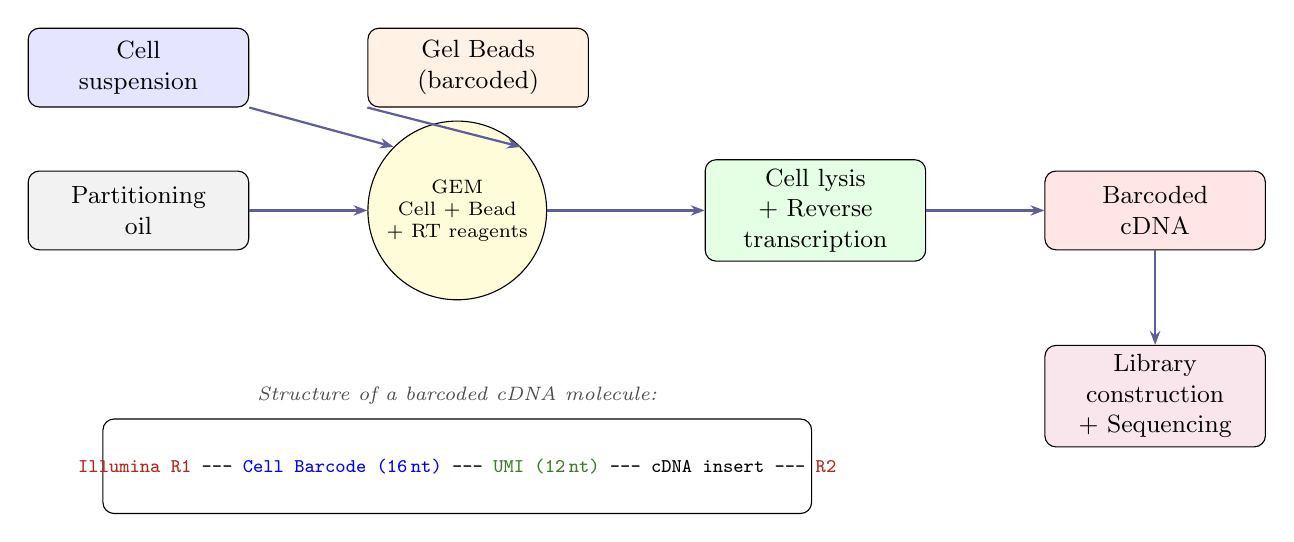
\begin{tikzpicture}[
  node distance=0.6cm and 0.3cm,
  every node/.style={font=\small},
  boxstep/.style={draw, rounded corners, minimum width=2.8cm, minimum height=1.0cm, align=center, font=\small},
  gem/.style={draw, circle, minimum size=1.8cm, fill=yellow!15, font=\scriptsize, align=center},
  arrow/.style={-{Stealth[length=5pt]}, thick, MidnightBlue!70},
  label/.style={font=\scriptsize\itshape, text=gray!60!black},
]

% Step 1: Cell suspension + Gel Beads + Oil
\node[boxstep, fill=blue!10] (cells) {Cell\\suspension};
\node[boxstep, fill=orange!10, right=1.5cm of cells] (beads) {Gel Beads\\(barcoded)};
\node[boxstep, fill=gray!10, below=0.8cm of cells] (oil) {Partitioning\\oil};

% GEM formation
\node[gem, right=1.5cm of oil] (gem) {GEM\\Cell + Bead\\+ RT reagents};

% Arrow to GEM
\draw[arrow] (cells.south east) -- (gem.north west);
\draw[arrow] (beads.south west) -- (gem.north east);
\draw[arrow] (oil.east) -- (gem.west);

% Inside GEM: cell lysis + RT
\node[boxstep, fill=green!10, right=2.0cm of gem] (rt) {Cell lysis\\+ Reverse\\transcription};
\draw[arrow] (gem.east) -- (rt.west);

% cDNA with barcodes
\node[boxstep, fill=red!10, right=1.5cm of rt] (cdna) {Barcoded\\cDNA};
\draw[arrow] (rt.east) -- (cdna.west);

% Library prep
\node[boxstep, fill=purple!10, below=1.2cm of cdna] (lib) {Library\\construction\\+ Sequencing};
\draw[arrow] (cdna.south) -- (lib.north);

% Barcode structure annotation
\node[below=1.5cm of gem, draw, rounded corners, fill=white, minimum width=9cm, minimum height=1.2cm] (barcode) {};
\node[font=\scriptsize\ttfamily, anchor=center] at (barcode.center) {
  \textcolor{BrickRed}{Illumina R1} ---
  \textcolor{blue}{Cell Barcode (16\,nt)} ---
  \textcolor{OliveGreen}{UMI (12\,nt)} ---
  \textcolor{black}{cDNA insert} ---
  \textcolor{BrickRed}{R2}
};
\node[label, above=0.05cm of barcode] {Structure of a barcoded cDNA molecule:};

\end{tikzpicture}
\caption{Schematic of the 10x Genomics Chromium droplet-based scRNA-seq
workflow. Single cells and gel beads are co-encapsulated in Gel Bead-in-Emulsions
(GEMs), where cell lysis and reverse transcription occur. Each gel bead carries
millions of oligonucleotide copies with a shared cell barcode and diverse UMIs.
The resulting cDNA is uniquely labeled with a cell barcode and a UMI for each
original mRNA molecule.}
\label{fig:scrnaseq:10x}
\end{figure}

\subsection{Gel Bead-in-Emulsions (GEMs)}

The core of the 10x Chromium system is the partitioning of single cells with
gel beads into nanoliter aqueous droplets suspended in oil (GEMs):

\begin{enumerate}[nosep]
  \item A microfluidic chip combines three streams: cell suspension, gel bead
    suspension, and partitioning oil.
  \item Each GEM ideally contains one cell and one gel bead. The vast majority
    of GEMs ($>$90\%) contain zero cells (empty) to minimize doublets (GEMs
    with two or more cells).
  \item The gel bead dissolves, releasing oligonucleotides into the droplet.
  \item Cell lysis releases mRNA, which is captured by oligo-dT sequences on
    the bead-derived oligonucleotides.
  \item Reverse transcription occurs within the GEM, producing first-strand
    cDNA tagged with the cell barcode and a unique molecular identifier (UMI).
\end{enumerate}

\subsection{Cell Barcodes and UMIs}

\begin{keyconcept}[title={Cell Barcodes and UMIs}]
\begin{description}[nosep]
  \item[Cell barcode (16\,nt):] Identifies which cell a cDNA molecule came from.
    All oligonucleotides on a single gel bead share the same cell barcode.
    Different gel beads have different barcodes. The 10x barcode whitelist
    contains $\sim$737,000 valid sequences (for 3$'$ v3/v3.1 chemistry).
  \item[UMI (12\,nt):] Unique Molecular Identifier. Each oligonucleotide on a
    bead has a random 12-mer UMI, enabling distinction between PCR duplicates
    and distinct original mRNA molecules. After PCR amplification, reads sharing
    the same cell barcode, UMI, and gene are collapsed to a single count,
    eliminating amplification bias.
\end{description}
\end{keyconcept}

\subsection{3$'$ vs.\ 5$'$ Gene Expression Chemistry}

\begin{description}[style=nextline]
  \item[3$'$ Gene Expression (GEX)] Captures the 3$'$ end of polyadenylated
    transcripts (within $\sim$500\,bp of the poly-A tail). Most commonly used
    chemistry. Sufficient for gene-level quantification and cell type
    identification. Cannot provide full-length transcript or isoform information.
  \item[5$'$ Gene Expression (GEX)] Captures the 5$'$ end of transcripts using
    template-switching. Enables simultaneous profiling of gene expression and
    immune receptor sequences (TCR/BCR V(D)J repertoires) from the same cells.
    Preferred for immunology studies.
\end{description}

\subsection{Cell Ranger Pipeline}

\software{Cell Ranger} is the standard 10x Genomics analysis pipeline that
processes raw Illumina BCL files into a gene-by-cell count matrix:

\begin{enumerate}[nosep]
  \item \texttt{cellranger mkfastq}: Demultiplexes BCL files into FASTQ files.
  \item \texttt{cellranger count}: Performs alignment (STAR), barcode counting,
    UMI deduplication, and generates the filtered feature-barcode matrix.
  \item \texttt{cellranger aggr}: Aggregates multiple \texttt{count} runs and
    normalizes across samples.
\end{enumerate}

The key output is the \textbf{filtered feature-barcode matrix}: a sparse
matrix where rows are genes ($\sim$33,000 for human) and columns are cell
barcodes that passed the cell-calling algorithm (EmptyDrops-like knee/inflection
point detection).

\subsection{Typical Throughput and Sequencing Recommendations}

\begin{itemize}[nosep]
  \item \textbf{Cells per reaction:} 500--10,000 (recommended loading for
    $\sim$0.8\% multiplet rate per 1,000 cells).
  \item \textbf{Sequencing depth:} 20,000--50,000 reads per cell for 3$'$ GEX.
    Higher depth yields diminishing returns for gene detection beyond
    $\sim$50,000 reads/cell.
  \item \textbf{Read configuration:} Read 1: 28\,bp (16\,bp cell barcode +
    12\,bp UMI); Index 1: 10\,bp (sample index); Read 2: 90\,bp (cDNA insert).
  \item \textbf{Expected genes per cell:} 2,000--6,000 median genes/cell,
    depending on cell type and sequencing depth.
\end{itemize}

\subsection{10x Chromium Flex (Fixed RNA Profiling)}

The Flex assay uses a probe-based approach to capture gene expression from
\emph{fixed} cells:

\begin{itemize}[nosep]
  \item Cells are fixed with paraformaldehyde, enabling sample banking and
    batch processing.
  \item Probe pairs hybridize to target mRNAs inside fixed cells; probes are
    ligated and then captured during GEM partitioning.
  \item Compatible with FFPE tissue sections (after deparaffinization).
  \item Supports sample multiplexing: up to 128 samples pooled in one Chromium
    run using probe-barcode-based demultiplexing.
  \item Lower background noise compared to 3$'$ GEX because probe-based
    detection avoids ambient RNA contamination.
\end{itemize}


% ---------------------------------------------------------------------------
\section{Key Computational Challenges}
\label{sec:scrnaseq:challenges}

\subsection{Sparsity and Dropout}

scRNA-seq data is extremely sparse: the median gene detection rate per cell is
only 15--30\% of expressed genes. Many genes that are truly expressed in a cell
are recorded as zero counts---a phenomenon called \textbf{dropout}. Dropout
arises from:

\begin{itemize}[nosep]
  \item Low mRNA capture efficiency ($\sim$5--15\% of transcripts in a cell for
    droplet-based methods).
  \item Stochastic sampling: with only $\sim$5,000--10,000 unique mRNA molecules
    detected per cell, lowly expressed genes are frequently missed.
  \item Shallow sequencing: not all cDNA molecules in the library are sequenced.
\end{itemize}

\begin{warningbox}
Dropout means that a zero count in scRNA-seq does not necessarily mean the gene
is not expressed. This has profound implications for analysis: methods that
treat zeros as true absence can produce misleading results. Many specialized
scRNA-seq statistical methods (e.g., MAST, scVI) explicitly model dropout or
use zero-inflated distributions.
\end{warningbox}

\subsection{Doublet Detection}

Doublets (or multiplets) occur when two or more cells are captured in the same
droplet or well. They appear as single ``cells'' with hybrid transcriptomes
that can create spurious intermediate populations or bridge clusters
artifactually.

The expected doublet rate for 10x Chromium is $\sim$0.8\% per 1,000 cells
loaded (e.g., loading 10,000 cells yields $\sim$8\% doublets).

\begin{description}[style=nextline]
  \item[\software{Scrublet}] Simulates doublets by combining random pairs of
    observed cell profiles and scores each real cell by its similarity to
    simulated doublets. Python-based.
  \item[\software{DoubletFinder}] Similar simulation-based approach implemented
    in R/Seurat. Requires parameter optimization (pK, expected doublet rate).
  \item[\software{scDblFinder}] Fast and accurate doublet detection using a
    gradient-boosted classifier trained on simulated doublets.
    R/Bioconductor-based.
\end{description}

\subsubsection{Doublet Detection: Principles and Expected Rates}
\label{subsec:scrnaseq:doublet_principles}

The fundamental principle behind simulation-based doublet detectors such as
\software{Scrublet} is straightforward:

\begin{enumerate}[nosep]
  \item \textbf{Simulate artificial doublets.} Randomly select pairs of observed
    cell profiles from the count matrix and sum their expression vectors. This
    creates synthetic doublets that mimic the transcriptomes of two co-captured
    cells.
  \item \textbf{Embed jointly.} Combine the real cells and simulated doublets,
    then perform dimensionality reduction (PCA followed by KNN graph
    construction) on the merged dataset.
  \item \textbf{Score each real cell.} For each observed cell, compute a
    \emph{doublet score} based on the local density of simulated doublets in
    its neighborhood. Cells surrounded by many simulated doublets are likely
    real doublets.
  \item \textbf{Threshold.} Apply a bimodal threshold (or a user-specified
    cutoff) to classify cells as singlets or doublets.
\end{enumerate}

The expected doublet rate for droplet-based platforms follows an approximately
linear relationship with loading density:
\begin{equation}
  \label{eq:scrnaseq:doubletrate}
  r_d \approx 0.008 \times \frac{n_{\text{cells}}}{1000}
\end{equation}
where $n_{\text{cells}}$ is the number of recovered cells per reaction. For
example, loading 5,000 cells yields an expected doublet rate of $\sim$4\%, while
10,000 cells gives $\sim$8\%. This formula assumes Poisson loading statistics
and is calibrated for the 10x Chromium platform.

\begin{warningbox}
Simulation-based doublet detectors excel at identifying \textbf{heterotypic
doublets} (two cells of different types, e.g., a T cell + a monocyte) because
these produce distinctive hybrid profiles. \textbf{Homotypic doublets} (two
cells of the same type) are nearly impossible to detect computationally because
their transcriptomes resemble a single cell with higher UMI counts. Homotypic
doublets inflate the apparent cell counts but typically do not create artifactual
clusters. When reporting cell numbers, account for both detected and undetected
(homotypic) doublets.
\end{warningbox}

\subsection{Ambient RNA Contamination}

During droplet generation, free-floating mRNA from lysed or damaged cells
(``soup'') is present in the cell suspension. This ambient RNA is captured in
every GEM, contaminating the transcriptomes of all cells with a background
signature (often enriched for highly expressed genes like hemoglobin in blood
or mitochondrial genes from damaged cells).

\begin{description}[style=nextline]
  \item[\software{SoupX}] Estimates the contamination fraction using the
    expression of genes expected to be cell-type-specific (e.g., hemoglobin in
    non-erythrocyte clusters). Subtracts estimated ambient counts.
  \item[\software{CellBender} (\texttt{remove-background})] Deep
    generative model that distinguishes cell-containing droplets from empty
    droplets and removes ambient RNA signal. Computationally intensive but
    highly effective.
  \item[\software{DecontX}] Bayesian method for ambient RNA decontamination
    that models each cell's expression as a mixture of its native profile and
    the ambient contamination profile.
\end{description}


% ---------------------------------------------------------------------------
\section{scRNA-seq Analysis Workflow}
\label{sec:scrnaseq:workflow}

The computational analysis of scRNA-seq data involves a well-established
sequence of steps, from raw data processing to biological interpretation.

% TikZ diagram: scRNA-seq analysis workflow
\begin{figure}[htbp]
\centering
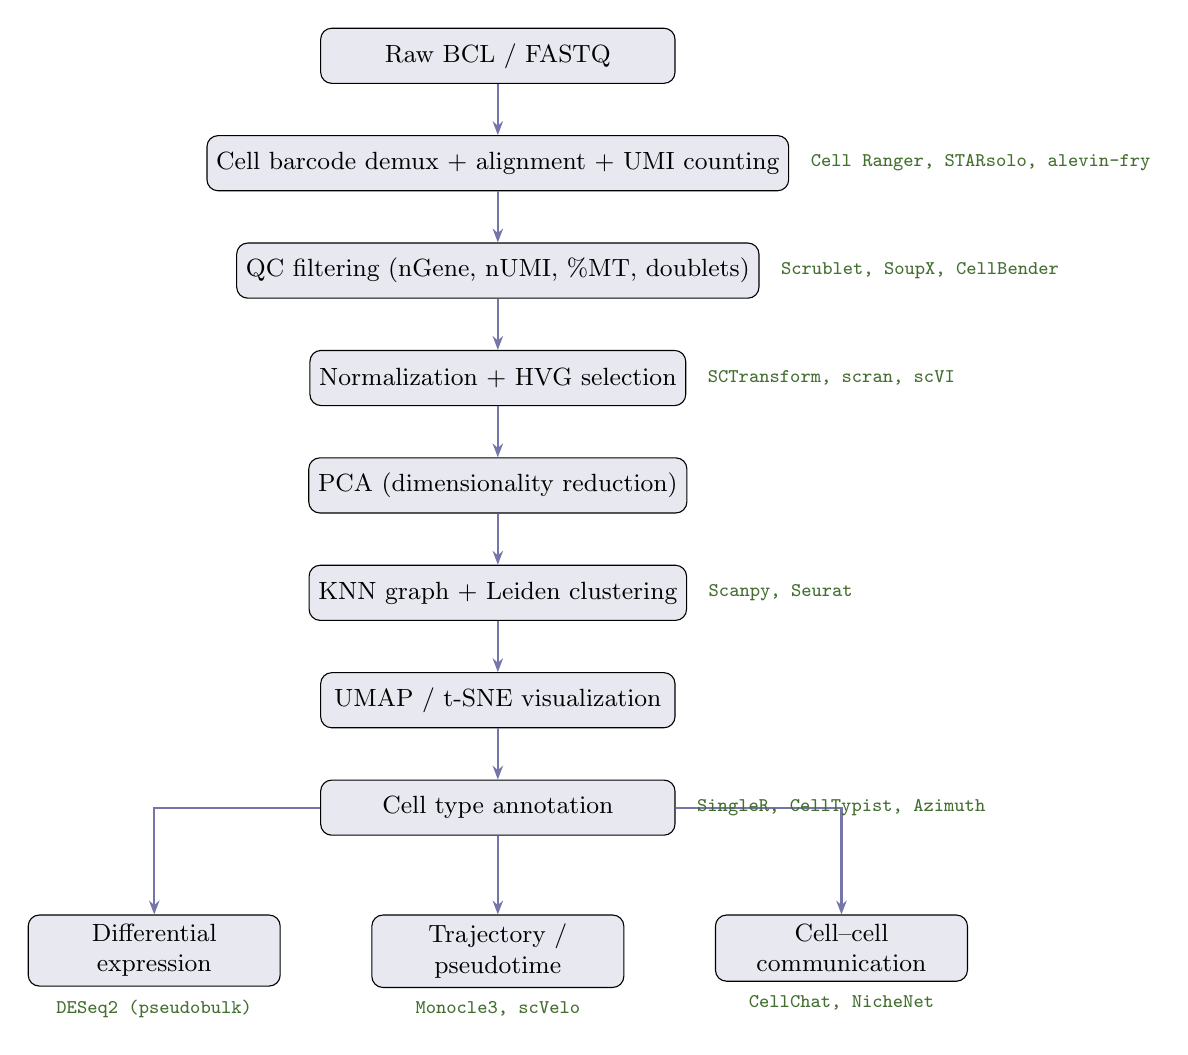
\begin{tikzpicture}[
  node distance=0.65cm,
  every node/.style={font=\small},
  boxstep/.style={draw, rounded corners, fill=MidnightBlue!10, minimum width=4.5cm, minimum height=0.7cm, align=center},
  tool/.style={font=\scriptsize\ttfamily, text=OliveGreen!80!black},
  arrow/.style={-{Stealth[length=5pt]}, thick, MidnightBlue!60},
]

\node[boxstep] (raw) {Raw BCL / FASTQ};
\node[boxstep, below=of raw] (count) {Cell barcode demux + alignment + UMI counting};
\node[boxstep, below=of count] (qc) {QC filtering (nGene, nUMI, \%MT, doublets)};
\node[boxstep, below=of qc] (norm) {Normalization + HVG selection};
\node[boxstep, below=of norm] (pca) {PCA (dimensionality reduction)};
\node[boxstep, below=of pca] (cluster) {KNN graph + Leiden clustering};
\node[boxstep, below=of cluster] (umap) {UMAP / t-SNE visualization};
\node[boxstep, below=of umap] (annot) {Cell type annotation};

% Downstream branches
\node[boxstep, below left=1.0cm and 0.5cm of annot, minimum width=3.2cm] (de) {Differential\\expression};
\node[boxstep, below=1.0cm of annot, minimum width=3.2cm] (traj) {Trajectory /\\pseudotime};
\node[boxstep, below right=1.0cm and 0.5cm of annot, minimum width=3.2cm] (comm) {Cell--cell\\communication};

% Arrows
\draw[arrow] (raw) -- (count);
\draw[arrow] (count) -- (qc);
\draw[arrow] (qc) -- (norm);
\draw[arrow] (norm) -- (pca);
\draw[arrow] (pca) -- (cluster);
\draw[arrow] (cluster) -- (umap);
\draw[arrow] (umap) -- (annot);
\draw[arrow] (annot) -| (de);
\draw[arrow] (annot) -- (traj);
\draw[arrow] (annot) -| (comm);

% Tool annotations
\node[tool, right=0.15cm of count] {Cell Ranger, STARsolo, alevin-fry};
\node[tool, right=0.15cm of qc] {Scrublet, SoupX, CellBender};
\node[tool, right=0.15cm of norm] {SCTransform, scran, scVI};
\node[tool, right=0.15cm of cluster] {Scanpy, Seurat};
\node[tool, right=0.15cm of annot] {SingleR, CellTypist, Azimuth};
\node[tool, below=0.05cm of de] {\scriptsize\ttfamily DESeq2 (pseudobulk)};
\node[tool, below=0.05cm of traj] {\scriptsize\ttfamily Monocle3, scVelo};
\node[tool, below=0.05cm of comm] {\scriptsize\ttfamily CellChat, NicheNet};

\end{tikzpicture}
\caption{Standard computational workflow for scRNA-seq analysis. After
generating a cell-by-gene count matrix, cells are filtered, normalized,
dimensionality-reduced, clustered, and annotated. Downstream analyses include
differential expression, trajectory inference, and cell--cell communication.}
\label{fig:scrnaseq:workflow}
\end{figure}

\subsection{Raw Data Processing}

\begin{description}[style=nextline]
  \item[\software{Cell Ranger}] The default pipeline for 10x Chromium data (see
    \cref{sec:scrnaseq:10x}). Closed-source but free. Produces the filtered
    count matrix and a web summary report.
  \item[\software{STARsolo}] Open-source alternative to Cell Ranger, built into
    the STAR aligner. Produces equivalent results with greater flexibility and
    often faster run time. Supports 10x, Drop-seq, and other barcode schemes.
  \item[\software{alevin-fry} (Salmon)] Lightweight mapping-based quantification
    for scRNA-seq. Uses the Salmon quasi-mapping engine with barcode-aware
    processing. Produces a count matrix compatible with downstream tools. The
    \software{simpleaf} wrapper simplifies execution.
\end{description}

\subsection{Quality Control and Filtering}

After generating the raw count matrix, per-cell QC metrics are computed and
cells failing quality thresholds are removed:

\begin{itemize}[nosep]
  \item \textbf{Number of genes detected (nGene):} Cells with very few genes
    ($< 200$--500) are likely empty droplets or debris.
  \item \textbf{Number of UMIs (nUMI / nCount):} Total counts per cell.
    Extremely high values may indicate doublets.
  \item \textbf{Percentage of mitochondrial reads (\%MT):} High mitochondrial
    fraction ($> 10$--20\%, depending on tissue) indicates dying or damaged
    cells whose cytoplasmic mRNA has leaked out while mitochondrial mRNA
    (enclosed in a double membrane) is retained.
  \item \textbf{Percentage of ribosomal protein genes (\%Ribo):} Can help
    identify low-quality cells or specific cell types.
  \item \textbf{Doublet scores:} From Scrublet, DoubletFinder, or scDblFinder.
\end{itemize}

\begin{tipbox}
QC thresholds should be adapted to the tissue and experiment. Brain tissue
typically has higher mitochondrial content than PBMCs. Use distribution-based
thresholds (e.g., $> 3$ median absolute deviations from the median) rather
than fixed cutoffs when possible. The \software{scater} package in R provides
automated outlier detection with \texttt{isOutlier()}.
\end{tipbox}

\subsection{Normalization}

Raw UMI counts must be normalized to account for differences in sequencing
depth (total UMIs) across cells.

\begin{description}[style=nextline]
  \item[Log-normalization (Seurat default)] Divide each cell's counts by total
    UMIs, multiply by a scale factor (default 10,000), and log-transform:
    $\log_2(\text{counts}/\text{total} \times 10{,}000 + 1)$. Simple and
    widely used.
  \item[\software{scran} pooling-based normalization] Pools cells into groups,
    estimates pool-based size factors, and deconvolves to per-cell size factors.
    More robust than simple library-size normalization because it handles the
    sparsity of single-cell data.
  \item[\software{SCTransform} (Seurat v3+)] Fits a regularized negative
    binomial regression model to each gene as a function of total UMIs. Replaces
    both normalization and variance stabilization in a single step. Handles
    the mean-variance relationship better than log-normalization for downstream
    analyses (PCA, clustering).
  \item[\software{scVI} (scvi-tools)] Deep generative model (variational
    autoencoder) that models the count generation process, implicitly handling
    normalization, batch effects, and dropout simultaneously.
\end{description}

\subsection{Feature Selection: Highly Variable Genes}

Not all $\sim$20,000+ detected genes are informative for distinguishing cell
types. Feature selection identifies \textbf{highly variable genes (HVGs)}---those
with expression variation exceeding what is expected from sampling noise.

\begin{itemize}[nosep]
  \item Seurat: fits a variance-stabilizing transformation and selects the top
    2,000--5,000 genes by residual variance.
  \item Scanpy: uses the method of Zheng et al.\ or the Seurat-style approach
    to identify HVGs.
  \item Only HVGs are used for dimensionality reduction and clustering,
    reducing noise and computation.
\end{itemize}

\subsection{Dimensionality Reduction}

\begin{description}[style=nextline]
  \item[PCA (Principal Component Analysis)] Linear dimensionality reduction.
    Typically the first 20--50 principal components are retained, capturing
    the major axes of variation. PCA is performed on the HVG expression matrix.
  \item[t-SNE (t-distributed Stochastic Neighbor Embedding)] Non-linear
    dimensionality reduction that preserves local structure. Produces 2D
    embeddings widely used for visualization. Sensitive to hyperparameters
    (perplexity). Does not preserve global distances.
  \item[UMAP (Uniform Manifold Approximation and Projection)] Non-linear
    method that preserves both local and (approximately) global structure.
    Faster than t-SNE and currently the most popular visualization method
    for scRNA-seq. Operates on the PCA-reduced space (not raw expression).
\end{description}

\begin{warningbox}
t-SNE and UMAP are visualization tools, not analytical methods. Do not perform
clustering on t-SNE/UMAP coordinates. Cluster on the PCA space or the shared
nearest neighbor (SNN) graph. Distances and apparent cluster sizes in t-SNE/UMAP
plots can be misleading.
\end{warningbox}

\subsection{Mathematical Foundations of t-SNE and UMAP}
\label{subsec:scrnaseq:tsne_umap_math}

Although t-SNE and UMAP are often treated as black-box visualization tools,
understanding their mathematical principles is essential for interpreting their
output correctly and tuning hyperparameters.

\subsubsection{t-SNE: t-distributed Stochastic Neighbor Embedding}

t-SNE operates in two stages. First, in the high-dimensional PCA space, pairwise
similarities are converted into conditional probabilities. The similarity of
point $x_j$ to point $x_i$ is defined as:
\begin{equation}
  \label{eq:scrnaseq:tsne_pij}
  p_{j|i} = \frac{\exp\!\bigl(-\|x_i - x_j\|^2 / 2\sigma_i^2\bigr)}
    {\sum_{k \neq i} \exp\!\bigl(-\|x_i - x_k\|^2 / 2\sigma_i^2\bigr)}
\end{equation}
where $\sigma_i$ is chosen such that the perplexity of the conditional
distribution matches a user-specified value (typically 30). The perplexity
controls the effective number of neighbors considered for each point.

The joint probability matrix is symmetrized as
$p_{ij} = (p_{j|i} + p_{i|j}) / (2n)$. In the low-dimensional embedding
(2D), similarities are modeled using a Student's $t$-distribution with one
degree of freedom (Cauchy distribution):
\begin{equation}
  \label{eq:scrnaseq:tsne_qij}
  q_{ij} = \frac{(1 + \|y_i - y_j\|^2)^{-1}}
    {\sum_{k \neq l} (1 + \|y_k - y_l\|^2)^{-1}}
\end{equation}
where $y_i, y_j$ are the low-dimensional coordinates. The heavy tails of the
$t$-distribution allow nearby points to be modeled faithfully while pushing
dissimilar points further apart, alleviating the ``crowding problem'' that
affects Gaussian-based methods like classical SNE.

t-SNE minimizes the Kullback--Leibler divergence between $P$ and $Q$:
\begin{equation}
  \label{eq:scrnaseq:tsne_kl}
  KL(P \| Q) = \sum_i \sum_{j \neq i} p_{ij}
    \log \frac{p_{ij}}{q_{ij}}
\end{equation}
via gradient descent. The asymmetry of KL divergence means that t-SNE penalizes
placing similar points far apart (``tearing'' neighborhoods) more heavily than
placing dissimilar points close together. This is why t-SNE excels at preserving
local structure but can distort global distances.

\subsubsection{UMAP: Uniform Manifold Approximation and Projection}

UMAP is grounded in topological data analysis and Riemannian geometry. Its key
steps are:

\begin{enumerate}[nosep]
  \item \textbf{Fuzzy simplicial set construction.} For each point $x_i$, UMAP
    finds its $k$ nearest neighbors and converts distances into membership
    strengths using a smooth kernel:
    \begin{equation}
      \label{eq:scrnaseq:umap_weight}
      w_{ij} = \exp\!\left(-\frac{d(x_i, x_j) - \rho_i}{\sigma_i}\right)
    \end{equation}
    where $\rho_i$ is the distance to the nearest neighbor of $x_i$ (ensuring
    local connectivity) and $\sigma_i$ is scaled to match the desired number of
    neighbors. These weights are symmetrized to form a fuzzy simplicial set
    (weighted graph) representing the topological structure of the data.
  \item \textbf{Low-dimensional optimization.} UMAP initializes a low-dimensional
    embedding (typically using spectral initialization on the fuzzy graph
    Laplacian) and optimizes it by minimizing a \textbf{cross-entropy loss}
    between the high-dimensional and low-dimensional fuzzy sets:
    \begin{equation}
      \label{eq:scrnaseq:umap_loss}
      \mathcal{L} = \sum_{(i,j)} \Bigl[
        w_{ij} \log\!\frac{w_{ij}}{v_{ij}}
        + (1 - w_{ij}) \log\!\frac{1 - w_{ij}}{1 - v_{ij}}
      \Bigr]
    \end{equation}
    where $v_{ij} = (1 + a \|y_i - y_j\|^{2b})^{-1}$ is the low-dimensional
    similarity, with $a$ and $b$ determined by the \texttt{min\_dist} parameter.
  \item \textbf{Stochastic gradient descent with negative sampling.} Rather than
    computing all pairwise interactions, UMAP uses negative sampling to
    approximate the repulsive term, making it substantially faster than t-SNE
    for large datasets ($\mathcal{O}(n)$ per epoch vs.\ $\mathcal{O}(n^2)$ for
    exact t-SNE).
\end{enumerate}

\begin{keyconcept}[title={t-SNE vs.\ UMAP: Key Differences}]
\begin{itemize}[nosep]
  \item \textbf{Global structure:} UMAP's cross-entropy loss includes a
    repulsive term for dissimilar points, better preserving global relationships
    (relative cluster positions) compared to t-SNE's KL divergence.
  \item \textbf{Speed:} UMAP is typically 5--50$\times$ faster than t-SNE for
    datasets with $>$50,000 cells, due to negative sampling and graph-based
    initialization.
  \item \textbf{Reproducibility:} UMAP with fixed random seed produces
    consistent embeddings; t-SNE results can vary substantially between runs.
  \item \textbf{Key hyperparameters:} For t-SNE, perplexity (30--50 typical);
    for UMAP, \texttt{n\_neighbors} (15--30) and \texttt{min\_dist}
    (0.1--0.5). Both should be explored rather than left at defaults.
\end{itemize}
\end{keyconcept}

\subsection{Clustering}

Graph-based clustering is the standard approach for scRNA-seq:

\begin{enumerate}[nosep]
  \item Construct a k-nearest neighbor (KNN) graph in PCA space. Each cell is a
    node; edges connect cells to their $k$ nearest neighbors.
  \item Refine edge weights using shared nearest neighbors (SNN graph) or
    Jaccard similarity.
  \item Apply a community detection algorithm:
    \begin{itemize}[nosep]
      \item \textbf{Louvain algorithm:} Optimizes modularity; fast but can
        produce poorly connected clusters.
      \item \textbf{Leiden algorithm:} Improved version of Louvain that
        guarantees well-connected communities. Generally preferred.
    \end{itemize}
  \item The \texttt{resolution} parameter controls the granularity of
    clustering: higher values produce more clusters. There is no single
    ``correct'' resolution; it should be guided by biological knowledge.
\end{enumerate}

\subsection{Cell Type Annotation}

Assigning biological identity to clusters is one of the most critical---and
most subjective---steps in scRNA-seq analysis.

\begin{description}[style=nextline]
  \item[Manual annotation] Examine marker genes for each cluster (e.g.,
    \gene{CD3D}/\gene{CD3E} for T cells, \gene{MS4A1}/\gene{CD79A} for B
    cells, \gene{LYZ}/\gene{CD14} for monocytes). Requires domain expertise.
    The \texttt{FindAllMarkers} function in Seurat and
    \texttt{sc.tl.rank\_genes\_groups} in Scanpy identify cluster-specific
    marker genes.
  \item[\software{SingleR}] Automated annotation by correlating each cell's
    expression profile to reference transcriptomic datasets (e.g., Human Primary
    Cell Atlas, Monaco Immune Data, Blueprint Encode). R-based.
  \item[\software{CellTypist}] Machine-learning-based classifier trained on
    large reference datasets. Pre-trained models for immune cells, brain cells,
    and pan-tissue atlases. Python-based.
  \item[\software{scType}] Fully automated cell type annotation using
    curated marker gene databases. R-based; no reference dataset required.
  \item[\software{Azimuth}] Web-based and R-based tool from the Seurat
    developers. Uses reference mapping to project query cells onto well-curated
    reference atlases (PBMC, lung, motor cortex, etc.). Provides both coarse
    and fine-grained cell type labels with confidence scores.
\end{description}

\subsection{Differential Expression}

Identifying genes that are differentially expressed between clusters or
conditions requires methods appropriate for the distributional properties of
scRNA-seq data:

\begin{description}[style=nextline]
  \item[Wilcoxon rank-sum test] Non-parametric; the default in both Seurat and
    Scanpy. Fast and performs reasonably well for cluster markers but does not
    account for the hierarchical structure of cells within samples.
  \item[\software{MAST}] Hurdle model that jointly models the rate of
    expression (logistic regression for zero vs.\ non-zero) and the expression
    level (linear model for non-zero values). Accounts for cellular detection
    rate as a confounding variable.
  \item[Pseudobulk approaches] Aggregate counts per cell type per biological
    replicate, then apply bulk DE tools (DESeq2, edgeR). This approach correctly
    treats biological replicates as the unit of inference (not individual
    cells) and has been shown to have the best calibrated false discovery rates
    in recent benchmarks. \textbf{Recommended for comparing conditions (e.g.,
    treatment vs.\ control) when biological replicates are available.}
\end{description}

\begin{keyconcept}[title={The Pseudobulk Principle}]
In a scRNA-seq experiment with multiple biological samples, individual cells
are not independent observations---cells from the same sample share the same
biological variation. Treating each cell as an independent replicate inflates
the sample size artificially and leads to extreme $p$-value inflation. The
solution is pseudobulk aggregation: sum counts across cells of the same type
within each biological replicate, then use bulk DE methods on the resulting
replicate-level counts.
\end{keyconcept}

\subsection{Trajectory Analysis and Pseudotime}

Many biological processes (differentiation, activation, disease progression)
involve continuous changes in gene expression rather than discrete states.
Trajectory analysis orders cells along a ``pseudotime'' axis that recapitulates
the dynamic process.

\begin{description}[style=nextline]
  \item[\software{Monocle3}] Learns a principal graph (trajectory) through the
    UMAP embedding using reversed graph embedding. Assigns each cell a
    pseudotime value representing its position along the trajectory. Supports
    branching trajectories for divergent differentiation paths.
  \item[\software{Slingshot}] Fits smooth curves through PCA or diffusion map
    space. Uses cluster information to define trajectory start and end points.
    Well-suited for simpler, tree-like trajectories.
  \item[\software{scVelo}] Infers RNA velocity---the time derivative of gene
    expression---from the ratio of spliced to unspliced mRNA counts in each
    cell. RNA velocity vectors indicate the future transcriptional state of
    each cell, providing directionality to trajectories.
  \item[\software{CellRank}] Combines RNA velocity with expression similarity
    to compute transition probabilities between cells. Identifies initial and
    terminal states and the most likely differentiation fates using Markov chain
    analysis.
\end{description}

\subsubsection{RNA Velocity: Mathematical Framework}
\label{subsec:scrnaseq:rna_velocity}

RNA velocity exploits the fact that standard scRNA-seq protocols capture both
spliced (mature) and unspliced (intron-containing) mRNA molecules. The ratio
between unspliced and spliced counts provides information about the
\emph{direction} of transcriptional change for each gene in each cell.

The core dynamical model for a single gene describes the time evolution of
unspliced ($u$) and spliced ($s$) mRNA abundances:
\begin{align}
  \label{eq:scrnaseq:velocity_unspliced}
  \frac{du}{dt} &= \alpha(t) - \beta\, u \\
  \label{eq:scrnaseq:velocity_spliced}
  \frac{ds}{dt} &= \beta\, u - \gamma\, s
\end{align}
where $\alpha(t)$ is the transcription rate, $\beta$ is the splicing rate
(conversion of unspliced to spliced mRNA), and $\gamma$ is the degradation rate
of spliced mRNA. The RNA \emph{velocity} for each gene is defined as $ds/dt$,
representing the expected rate of change of the mature mRNA.

\begin{description}[style=nextline]
  \item[Steady-state model (\software{velocyto})] Assumes that genes are in
    either an induction or repression phase, each at approximate steady state.
    At steady state, $ds/dt = 0$ implies $\beta u = \gamma s$, so the expected
    ratio is $u/s = \gamma/\beta$. Cells deviating above this ratio (excess
    unspliced) are actively upregulating the gene; cells below are downregulating
    it. The velocity is estimated as:
    \begin{equation}
      \label{eq:scrnaseq:velocity_ss}
      v_g = \beta\, u_g - \gamma_g\, s_g
    \end{equation}
    where $\gamma_g$ is estimated from the slope of the upper quantile of the
    $u$ vs.\ $s$ phase portrait.
  \item[Dynamical model (\software{scVelo})] Relaxes the steady-state assumption
    by solving the full system of ODEs (Equations
    \ref{eq:scrnaseq:velocity_unspliced}--\ref{eq:scrnaseq:velocity_spliced})
    using an expectation-maximization algorithm. This jointly infers the kinetic
    parameters $\alpha$, $\beta$, $\gamma$, and a latent time for each cell,
    providing a more accurate velocity field for genes that are not at steady
    state (e.g., during rapid transitions).
  \item[Multi-omic velocity (\software{MultiVelo})] Extends the velocity
    framework to incorporate chromatin accessibility (from multi-omic
    ATAC + RNA data), modeling the cascade from chromatin opening to unspliced
    to spliced mRNA.
\end{description}

\begin{tipbox}
RNA velocity estimates are gene-specific vectors in expression space. To
visualize them on a UMAP or t-SNE embedding, the high-dimensional velocity
vectors are projected onto the 2D embedding by computing the correlation between
each cell's velocity and the expression difference to its neighbors. Arrows on
the embedding indicate the predicted direction of transcriptional change, not
physical movement.
\end{tipbox}

\subsection{Cell--Cell Communication}

\begin{description}[style=nextline]
  \item[\software{CellChat}] Infers intercellular communication networks from
    scRNA-seq data using a curated database of ligand--receptor interactions
    (including multimeric complexes). Models communication probability based on
    the law of mass action and identifies significant signaling pathways between
    cell types.
  \item[\software{NicheNet}] Predicts which ligands from sender cells best
    explain gene expression changes in receiver cells, integrating prior
    knowledge of signaling and gene regulatory networks.
  \item[\software{LIANA}] A framework that benchmarks and combines multiple
    cell--cell communication tools (CellPhoneDB, CellChat, NATMI,
    SingleCellSignalR, etc.) to produce consensus interaction scores.
\end{description}

\subsection{Gene Regulatory Network Inference}

\begin{description}[style=nextline]
  \item[\software{SCENIC / pySCENIC}] \textbf{S}ingle-\textbf{C}ell r\textbf{E}gulatory
    \textbf{N}etwork \textbf{I}nference and \textbf{C}lustering. A three-step
    pipeline:
    \begin{enumerate}[nosep]
      \item Co-expression modules: identify genes co-expressed with each
        transcription factor (TF) using GRNBoost2 or GENIE3.
      \item Regulon pruning: retain only target genes with TF binding motifs
        in their regulatory regions (cis-regulatory analysis using RcisTarget
        or pycisTarget).
      \item Regulon activity scoring: quantify the activity of each regulon
        (TF + targets) in each cell using AUCell.
    \end{enumerate}
    SCENIC regulon activity provides a biologically interpretable dimensionality
    reduction and can reveal TF-driven cell states invisible in gene expression
    alone.
\end{description}


% ---------------------------------------------------------------------------
\section{Analysis Frameworks: Scanpy vs.\ Seurat}
\label{sec:scrnaseq:frameworks}

Two comprehensive frameworks dominate the scRNA-seq analysis ecosystem:

\begin{table}[htbp]
\centering
\caption{Comparison of the Scanpy (Python) and Seurat (R) scRNA-seq analysis
frameworks.}
\label{tab:scrnaseq:frameworks}
\small
\begin{tabularx}{\textwidth}{lXX}
\toprule
\textbf{Feature} & \textbf{Scanpy (Python)} & \textbf{Seurat (R)} \\
\midrule
Language & Python & R \\
Current version & Scanpy 1.10+ & Seurat v5 \\
Data structure & AnnData (\texttt{.h5ad}) & SeuratObject / BPCells \\
Core functions & Preprocessing, clustering, DE, visualization & Preprocessing, clustering, DE, visualization \\
Normalization & Log-norm, scran (via rpy2) & Log-norm, SCTransform, sketch-based \\
Integration & scVI, scANVI, BBKNN, Harmony & CCA, RPCA, Harmony, scVI bridge \\
Scalability & Excellent (sparse arrays, GPU via rapids-singlecell) & Improved in v5 (BPCells on-disk), sketch-based \\
Visualization & Matplotlib-based (highly customizable) & ggplot2-based (publication-ready) \\
Ecosystem & scvi-tools, squidpy, CellRank, decoupler & Signac, Azimuth, BPCells \\
Community & Strong in computational biology / ML & Strong in biomedical research \\
\bottomrule
\end{tabularx}
\end{table}

\begin{tipbox}
Both frameworks are excellent and actively maintained. Choose based on your
language proficiency and collaborators' preferences. Many analyses use both:
Scanpy for preprocessing and Seurat for visualization (or vice versa).
Conversion between AnnData (\texttt{.h5ad}) and SeuratObject formats is
straightforward using the \software{SeuratDisk} or \software{MuDataSeurat}
packages.
\end{tipbox}


% ---------------------------------------------------------------------------
\section{Integration of Multiple Datasets}
\label{sec:scrnaseq:integration}

Combining scRNA-seq datasets from different experiments, batches, or
technologies is essential for large-scale analyses but is complicated by
batch effects. Integration methods aim to place cells from different batches
into a common embedding while preserving biological variation.

\begin{description}[style=nextline]
  \item[\software{Harmony}] Fast linear integration that iteratively adjusts
    PCA embeddings to remove batch effects while preserving biological clusters.
    Extremely popular due to speed and simplicity. Works as a post-PCA
    correction.
  \item[\software{scVI} (Variational Inference)] Deep generative model
    (variational autoencoder) that learns a batch-corrected latent space.
    Handles complex batch effects and provides uncertainty estimates. The gold
    standard for large, complex integration tasks.
  \item[\software{BBKNN} (Batch Balanced KNN)] Modifies the KNN graph
    construction to balance neighbors across batches. Simple and effective;
    does not modify the expression matrix.
  \item[Seurat integration (CCA/RPCA)] Identifies ``anchors'' (mutual nearest
    neighbors) between datasets using canonical correlation analysis (CCA) or
    reciprocal PCA (RPCA). Anchors guide the alignment of datasets into a
    common space. RPCA is faster and recommended for datasets with partially
    overlapping cell types.
\end{description}

\begin{warningbox}
Over-integration can remove genuine biological differences between datasets.
Always verify that integration preserved known biological signals (e.g., marker
gene expression for expected cell types). Compare integrated and non-integrated
results critically, and use integration metrics (kBET, LISI, silhouette width)
to quantify batch mixing and biological conservation.
\end{warningbox}

\subsection{Batch Correction Methods: A Detailed Comparison}
\label{subsec:scrnaseq:batch_correction}

Choosing the right integration method depends on dataset size, batch complexity,
and the importance of preserving subtle biological variation. The following table
summarizes the key properties of the most widely used methods:

\begin{table}[htbp]
\centering
\caption{Comparison of batch correction and integration methods for scRNA-seq.}
\label{tab:scrnaseq:batch_correction}
\small
\begin{tabularx}{\textwidth}{lXXXX}
\toprule
\textbf{Method} & \textbf{Approach} & \textbf{Speed} & \textbf{Preservation of biology} & \textbf{Notes} \\
\midrule
\software{Harmony} & Iterative soft clustering on PCA embeddings; adjusts cluster centroids across batches & Very fast ($<$1 min for 500k cells) & Good; may over-correct rare populations & Post-PCA; does not modify expression matrix; easy to use \\
MNN (Mutual Nearest Neighbors) & Identifies mutual nearest neighbor pairs across batches; computes correction vectors & Moderate & Good for conserved populations & Implemented in \software{batchelor} (R); foundational method \\
\software{scVI} & Variational autoencoder with batch as a covariate in the generative model & Slow (GPU recommended; minutes--hours) & Excellent; learns complex non-linear corrections & Produces a latent space, not corrected counts; best for complex multi-batch designs \\
\software{BBKNN} & Constructs a batch-balanced KNN graph by trimming neighbors per batch & Very fast & Good; minimal distortion of rare types & Corrects the graph, not the embedding or expression; use with Scanpy \\
\software{Scanorama} & Panoramic stitching inspired by image alignment; finds mutual nearest neighbors in SVD space & Fast (scales to millions of cells) & Good; robust to partially overlapping datasets & Can correct expression matrix directly; useful when datasets share only some cell types \\
\bottomrule
\end{tabularx}
\end{table}

\begin{keyconcept}[title={Metrics for Evaluating Integration Quality}]
Integration quality should be assessed along two orthogonal axes:
\begin{itemize}[nosep]
  \item \textbf{Batch mixing} (technical correction): Do cells of the same type
    from different batches intermingle? Measured by kBET (k-nearest neighbor
    batch effect test) and the iLISI (integration Local Inverse Simpson Index).
    Higher values indicate better batch mixing.
  \item \textbf{Biological conservation}: Are genuine cell types still
    distinguishable after integration? Measured by cLISI (cell-type LISI),
    silhouette width, and ARI (Adjusted Rand Index) against known labels.
    Over-integration reduces these metrics.
\end{itemize}
The \software{scIB} (single-cell Integration Benchmarking) framework provides a
standardized pipeline for computing these metrics and ranking integration methods
for a given dataset.
\end{keyconcept}


% ---------------------------------------------------------------------------
\section{Large-Scale Cell Atlases}
\label{sec:scrnaseq:atlases}

The field has moved from profiling individual tissues to constructing
organism-wide cell atlases:

\begin{description}[style=nextline]
  \item[Human Cell Atlas (HCA)] An international consortium aiming to create a
    comprehensive reference map of every human cell type. Spans dozens of organs
    and developmental stages. Data accessible via the HCA Data Portal.
  \item[Tabula Sapiens] A multi-organ, single-cell transcriptomic atlas of
    \species{Homo sapiens}. Profiled $\sim$500,000 cells from 24 organs of
    individual donors, enabling cross-tissue cell type comparisons.
  \item[Tabula Muris / Tabula Muris Senis] Mouse cell atlases covering 20+
    organs using both 10x Chromium (3$'$) and Smart-seq2 (full-length) protocols.
    Senis extends to aging, covering mice from 1 to 30 months.
  \item[CellxGene Census] Aggregated and harmonized single-cell data from
    multiple studies, providing programmatic access (Python/R APIs) to tens
    of millions of cells with standardized metadata and cell type annotations.
\end{description}


% ---------------------------------------------------------------------------
\section{Practical Considerations}
\label{sec:scrnaseq:practical}

\subsection{How Many Cells to Sequence?}

\begin{itemize}[nosep]
  \item \textbf{For common cell types:} 3,000--5,000 cells per sample is often
    sufficient.
  \item \textbf{For rare populations:} If a target cell type is $\sim$1\% of
    the sample, profiling 10,000--20,000 cells ensures $\sim$100--200 cells of
    that type.
  \item \textbf{For differential abundance testing:} Multiple biological
    replicates (n $\geq$ 3) are far more important than the number of cells per
    sample.
  \item \textbf{Trade-off:} More cells at lower depth vs.\ fewer cells at
    higher depth. For cell type identification, breadth (more cells) generally
    wins; for gene-level analyses within a cell type, depth matters more.
\end{itemize}

\subsection{Sequencing Depth Per Cell}

\begin{itemize}[nosep]
  \item \textbf{3$'$ 10x Chromium:} 20,000--50,000 reads per cell is standard.
    Beyond 50,000 reads, the number of newly detected genes saturates rapidly.
  \item \textbf{5$'$ 10x Chromium:} Similar depth for GEX; additional depth for
    V(D)J libraries ($\sim$5,000 reads/cell).
  \item \textbf{Smart-seq2:} 0.5--1 million reads per cell (full-length,
    no UMIs; deeper sequencing improves isoform detection).
  \item \textbf{Multiplexed experiments:} Calculate total reads as
    (cells $\times$ reads/cell) and ensure the sequencing run provides
    sufficient output.
\end{itemize}

\subsection{Tissue Dissociation Considerations}

Preparing a high-quality single-cell suspension is often the most challenging
step in a scRNA-seq experiment:

\begin{itemize}[nosep]
  \item \textbf{Enzymatic digestion:} Collagenase, trypsin, Liberase, or
    tissue-specific cocktails. Over-digestion kills cells; under-digestion
    yields clumps and debris.
  \item \textbf{Mechanical dissociation:} Gentle trituration or the
    Miltenyi gentleMACS for standardized processing.
  \item \textbf{Dead cell removal:} MACS dead cell removal kit or FACS-based
    viability gating (DAPI, 7-AAD, calcein AM).
  \item \textbf{Dissociation-induced artifacts:} Enzymatic digestion can
    activate stress-response genes (e.g., \gene{FOS}, \gene{JUN},
    \gene{HSPA1A}). Cold-active protease protocols or fixation-based approaches
    (10x Flex, FANS for nuclei) mitigate this.
  \item \textbf{Single-nucleus RNA-seq (snRNA-seq):} For tissues that cannot be
    dissociated into viable single cells (e.g., brain, adipose, archived frozen
    tissue), nuclei are isolated and profiled. Uses the same 10x Chromium
    platform with nuclei-specific protocols. Detects both cytoplasmic and
    nuclear RNA (more intronic reads).
\end{itemize}

\begin{warningbox}
Always check for dissociation-induced gene expression artifacts by examining
immediate-early gene expression across clusters. If stress genes (e.g.,
\gene{FOS}, \gene{JUN}, \gene{ATF3}) dominate the first principal components
or separate clusters, consider regressing them out or switching to a
cold-dissociation or nucleus-based protocol.
\end{warningbox}


% ---------------------------------------------------------------------------
\section{Comparison of scRNA-seq Platforms}
\label{sec:scrnaseq:comparison}

\begin{table}[htbp]
\centering
\caption{Comparison of major scRNA-seq platforms and methods.}
\label{tab:scrnaseq:platforms}
\small
\begin{tabularx}{\textwidth}{lXXXX}
\toprule
\textbf{Feature} & \textbf{10x Chromium 3$'$} & \textbf{Smart-seq2/3} & \textbf{Drop-seq} & \textbf{sci-RNA-seq3} \\
\midrule
Isolation & Droplet & FACS to plate & Droplet & Combinatorial indexing \\
Throughput & 500--10,000 cells & 96--384 cells & 2,000--10,000 cells & $>$100,000 cells \\
Sensitivity & 3,000--6,000 genes/cell & 5,000--10,000 genes/cell & 1,500--3,000 genes/cell & 1,000--2,000 genes/cell \\
Coverage & 3$'$ end & Full-length & 3$'$ end & 3$'$ end \\
UMIs & Yes (12\,nt) & No (SS2) / Yes (SS3) & Yes & Yes \\
Cost per cell & \$0.10--0.50 & \$5--20 & \$0.05--0.20 & \$0.01--0.05 \\
Equipment & Chromium Controller & FACS + thermocycler & Custom microfluidics & Standard lab equipment \\
Isoform info & No & Yes & No & No \\
Multiplexing & CellPlex, Flex & Limited & Limited & Built-in \\
Best use case & Standard profiling & Deep per-cell profiling & Budget-friendly scaling & Organism-scale atlases \\
\bottomrule
\end{tabularx}
\end{table}


% ---------------------------------------------------------------------------
\section{Snakemake Workflow for scRNA-seq}
\label{sec:scrnaseq:snakemake}

\begin{lstlisting}[language=Python, caption={Snakemake workflow for 10x
Chromium scRNA-seq analysis using STARsolo and Scanpy.},
label={lst:scrnaseq:snakemake}, float=htbp]
# Snakefile for scRNA-seq Analysis (10x Chromium)
# ================================================
# Pipeline: STARsolo -> Scanpy (QC, norm, cluster, annotate)

import pandas as pd

configfile: "config/config.yaml"

samples = pd.read_csv(config["samples"], sep="\t")
SAMPLES = samples["sample"].tolist()

STAR_INDEX = config["star_index"]
WHITELIST  = config["barcode_whitelist"]

rule all:
    input:
        expand("results/starsolo/{sample}/Solo.out/"
               "Gene/filtered/matrix.mtx",
               sample=SAMPLES),
        "results/scanpy/integrated_analysis.h5ad",
        "results/scanpy/umap_celltypes.pdf",
        "results/multiqc/multiqc_report.html"

rule starsolo:
    input:
        r1="data/raw/{sample}_R1.fastq.gz",
        r2="data/raw/{sample}_R2.fastq.gz",
        index=STAR_INDEX,
        whitelist=WHITELIST
    output:
        bam="results/starsolo/{sample}/"
            "Aligned.sortedByCoord.out.bam",
        matrix="results/starsolo/{sample}/Solo.out/"
               "Gene/filtered/matrix.mtx",
        barcodes="results/starsolo/{sample}/Solo.out/"
                 "Gene/filtered/barcodes.tsv",
        features="results/starsolo/{sample}/Solo.out/"
                 "Gene/filtered/features.tsv",
        log="results/starsolo/{sample}/Log.final.out"
    threads: 12
    resources:
        mem_mb=40000
    params:
        prefix="results/starsolo/{sample}/",
        cb_len=16,
        umi_len=12
    conda: "envs/starsolo.yaml"
    shell:
        """
        STAR --runMode alignReads \
          --genomeDir {input.index} \
          --readFilesIn {input.r2} {input.r1} \
          --readFilesCommand zcat \
          --soloType CB_UMI_Simple \
          --soloCBwhitelist {input.whitelist} \
          --soloCBlen {params.cb_len} \
          --soloUMIlen {params.umi_len} \
          --soloFeatures Gene \
          --soloMultiMappers EM \
          --soloCellFilter EmptyDrops_CR \
          --outSAMtype BAM SortedByCoordinate \
          --outSAMattributes NH HI nM AS CR UR CB UB \
            GX GN \
          --outFileNamePrefix {params.prefix} \
          --runThreadN {threads} \
          --limitBAMsortRAM 30000000000
        """

rule doublet_detection:
    input:
        matrix="results/starsolo/{sample}/Solo.out/"
               "Gene/filtered/matrix.mtx"
    output:
        scores="results/doublets/{sample}_scores.csv"
    conda: "envs/scanpy.yaml"
    script:
        "scripts/run_scrublet.py"

rule scanpy_analysis:
    input:
        matrices=expand(
            "results/starsolo/{sample}/Solo.out/"
            "Gene/filtered/matrix.mtx",
            sample=SAMPLES),
        doublets=expand(
            "results/doublets/{sample}_scores.csv",
            sample=SAMPLES),
        sample_sheet=config["samples"]
    output:
        h5ad="results/scanpy/integrated_analysis.h5ad",
        umap="results/scanpy/umap_celltypes.pdf",
        markers="results/scanpy/marker_genes.csv",
        qc_report="results/scanpy/qc_violin_plots.pdf"
    conda: "envs/scanpy.yaml"
    script:
        "scripts/run_scanpy.py"

rule multiqc:
    input:
        expand("results/starsolo/{sample}/Log.final.out",
               sample=SAMPLES)
    output:
        "results/multiqc/multiqc_report.html"
    conda: "envs/qc.yaml"
    shell:
        "multiqc results/ -o results/multiqc/ --force"
\end{lstlisting}


% ---------------------------------------------------------------------------
\section{Nextflow Workflow for scRNA-seq}
\label{sec:scrnaseq:nextflow}

\begin{lstlisting}[language=Java, caption={Nextflow DSL2 workflow for 10x
Chromium scRNA-seq analysis using STARsolo and Scanpy.},
label={lst:scrnaseq:nextflow}, float=htbp]
#!/usr/bin/env nextflow
// scRNA-seq Analysis Pipeline (Nextflow DSL2)
// =============================================
// Pipeline: STARsolo -> Scrublet -> Scanpy

nextflow.enable.dsl = 2

params.reads        = "data/raw/*_{R1,R2}.fastq.gz"
params.star_index   = "resources/star_index"
params.whitelist    = "resources/3M-february-2018.txt"
params.sample_sheet = "config/samples.tsv"
params.outdir       = "results"

log.info """
=================================
 scRNA-seq Analysis Pipeline
=================================
 reads        : ${params.reads}
 STAR index   : ${params.star_index}
 whitelist    : ${params.whitelist}
 outdir       : ${params.outdir}
=================================
"""

process STARSOLO {
    tag "$sample_id"
    publishDir "${params.outdir}/starsolo/${sample_id}",
        mode: 'copy'
    cpus 12
    memory '40 GB'

    input:
    tuple val(sample_id), path(reads)
    path(star_index)
    path(whitelist)

    output:
    tuple val(sample_id),
        path("Solo.out/Gene/filtered/"),
        emit: filtered
    path("Log.final.out"), emit: log
    tuple val(sample_id),
        path("Aligned.sortedByCoord.out.bam"),
        emit: bam

    script:
    def (r1, r2) = reads
    """
    STAR --runMode alignReads \
      --genomeDir ${star_index} \
      --readFilesIn ${r2} ${r1} \
      --readFilesCommand zcat \
      --soloType CB_UMI_Simple \
      --soloCBwhitelist ${whitelist} \
      --soloCBlen 16 \
      --soloUMIlen 12 \
      --soloFeatures Gene \
      --soloMultiMappers EM \
      --soloCellFilter EmptyDrops_CR \
      --outSAMtype BAM SortedByCoordinate \
      --outSAMattributes NH HI nM AS CR UR CB UB \
        GX GN \
      --runThreadN ${task.cpus}
    """
}

process SCRUBLET {
    tag "$sample_id"
    publishDir "${params.outdir}/doublets", mode: 'copy'

    input:
    tuple val(sample_id), path(filtered_dir)

    output:
    tuple val(sample_id),
        path("${sample_id}_doublet_scores.csv"),
        emit: scores

    script:
    """
    python ${projectDir}/bin/run_scrublet.py \
      --input ${filtered_dir} \
      --output ${sample_id}_doublet_scores.csv
    """
}

process SCANPY_ANALYSIS {
    publishDir "${params.outdir}/scanpy", mode: 'copy'
    cpus 4
    memory '16 GB'

    input:
    path(filtered_dirs)
    path(doublet_scores)
    path(sample_sheet)

    output:
    path("integrated_analysis.h5ad"), emit: h5ad
    path("umap_celltypes.pdf"),       emit: umap
    path("marker_genes.csv"),         emit: markers
    path("qc_violin_plots.pdf"),      emit: qc

    script:
    """
    python ${projectDir}/bin/run_scanpy.py \
      --input_dirs ${filtered_dirs} \
      --doublets ${doublet_scores} \
      --samples ${sample_sheet} \
      --outdir .
    """
}

process MULTIQC {
    publishDir "${params.outdir}/multiqc", mode: 'copy'

    input:
    path('*')

    output:
    path("multiqc_report.html")

    script:
    """
    multiqc . -o . --force
    """
}

workflow {
    reads_ch = Channel
        .fromFilePairs(params.reads, checkIfExists: true)

    star_index = Channel.fromPath(params.star_index)
    whitelist  = Channel.fromPath(params.whitelist)

    // Align and quantify
    STARSOLO(reads_ch, star_index.collect(),
             whitelist.collect())

    // Detect doublets per sample
    SCRUBLET(STARSOLO.out.filtered)

    // Integrated analysis
    SCANPY_ANALYSIS(
        STARSOLO.out.filtered
            .map { it[1] }.collect(),
        SCRUBLET.out.scores
            .map { it[1] }.collect(),
        Channel.fromPath(params.sample_sheet)
    )

    // QC report
    MULTIQC(STARSOLO.out.log.collect())
}
\end{lstlisting}

\begin{tipbox}
For production scRNA-seq analysis, the \software{nf-core/scrnaseq} pipeline
provides a comprehensive Nextflow workflow supporting Cell Ranger, STARsolo,
alevin-fry (Salmon), and kallisto-bustools as quantification backends, with
automatic whitelist selection and extensive QC reporting.
\end{tipbox}


% ---------------------------------------------------------------------------
\section{Chapter Summary}
\label{sec:scrnaseq:summary}

Single-cell RNA sequencing has revolutionized our ability to dissect cellular
heterogeneity and has become an indispensable tool in modern biology. In this
chapter we covered:

\begin{itemize}[nosep]
  \item Why single-cell resolution is necessary and what bulk RNA-seq misses.
  \item The historical development of scRNA-seq technologies from 2009 to the
    present.
  \item Cell isolation methods: FACS, microfluidics, droplet-based (10x
    Chromium, Drop-seq, inDrop), combinatorial indexing (sci-RNA-seq, SPLiT-seq),
    and plate-based (Smart-seq2/3).
  \item The 10x Genomics Chromium system in detail: GEM formation, cell barcodes,
    UMIs, 3$'$ vs.\ 5$'$ chemistry, Cell Ranger, and the Flex assay.
  \item Computational challenges: sparsity/dropout, doublet detection, and
    ambient RNA contamination.
  \item The complete analysis workflow: raw data processing (Cell Ranger, STARsolo,
    alevin-fry), QC filtering, normalization (scran, SCTransform), feature
    selection (HVGs), dimensionality reduction (PCA, t-SNE, UMAP), graph-based
    clustering (Leiden/Louvain), cell type annotation, differential expression
    (pseudobulk recommended), trajectory analysis (Monocle3, scVelo),
    cell--cell communication (CellChat, NicheNet), and gene regulatory networks
    (SCENIC).
  \item Scanpy vs.\ Seurat frameworks, and dataset integration methods.
  \item Large-scale cell atlases: Human Cell Atlas, Tabula Sapiens, Tabula Muris.
  \item Practical workflows in both Snakemake and Nextflow.
\end{itemize}

The next chapter extends our view from dissociated single cells to cells in
their native tissue context with spatial transcriptomics (\cref{ch:spatial}).

% ==============================================================================
% Chapter 12: Spatial Transcriptomics
% ==============================================================================
\chapter{Spatial Transcriptomics}
\label{ch:spatial}

\begin{sourcebox}
The field is anchored here by the original array-based spatial transcriptomics report \cite{stahl2016}. Resolution, area, plex, sensitivity, and analysis-software claims for commercial systems require current product documentation and must not be compared as if they measured identical quantities.
\end{sourcebox}

\begin{keyconcept}
Spatial transcriptomics measures gene expression while preserving the physical
location of each measurement within a tissue section. By retaining spatial
context---lost in both bulk and dissociated single-cell RNA-seq---these
technologies reveal how cells are organized, how they communicate with their
neighbors, and how tissue architecture relates to function and disease.
\end{keyconcept}

% ---------------------------------------------------------------------------
\section{Why Spatial Context Matters}
\label{sec:spatial:why}

The human body is not a bag of cells: it is a precisely organized structure
where cellular function depends critically on spatial position. Conventional
scRNA-seq requires tissue dissociation, which destroys the spatial
relationships between cells. This loss has several consequences:

\begin{itemize}[nosep]
  \item \textbf{Tissue architecture is invisible:} The layered organization of
    the cortex, the crypt--villus axis of the intestine, and the zonal
    structure of the liver cannot be observed in dissociated data.
  \item \textbf{Cell neighborhoods are lost:} A tumor cell adjacent to a
    cytotoxic T cell behaves differently from one surrounded by
    immunosuppressive macrophages. Spatial context determines these
    interactions.
  \item \textbf{Gradients cannot be detected:} Morphogen gradients during
    development, oxygen gradients in tumors, and signaling gradients in wound
    healing require spatial measurement.
  \item \textbf{Rare niches are obscured:} Stem cell niches, germinal centers,
    and tertiary lymphoid structures are defined by their spatial organization
    as much as by their cell type composition.
  \item \textbf{Dissociation introduces artifacts:} Enzymatic digestion
    activates stress-response genes and selectively loses fragile cell types
    (neurons, adipocytes, syncytiotrophoblasts).
\end{itemize}

Spatial transcriptomics solves these problems by measuring gene expression
\emph{in situ}---within intact tissue sections.


% ---------------------------------------------------------------------------
\section{Categories of Spatial Technologies}
\label{sec:spatial:categories}

Spatial transcriptomics technologies can be broadly divided into three
categories based on their detection mechanism: sequencing-based methods that
capture RNA at defined spatial positions, imaging-based methods that visualize
individual RNA molecules, and in situ sequencing methods that read out RNA
sequences directly in tissue.

% TikZ diagram: Comparison of spatial transcriptomics approaches
\begin{figure}[htbp]
\centering
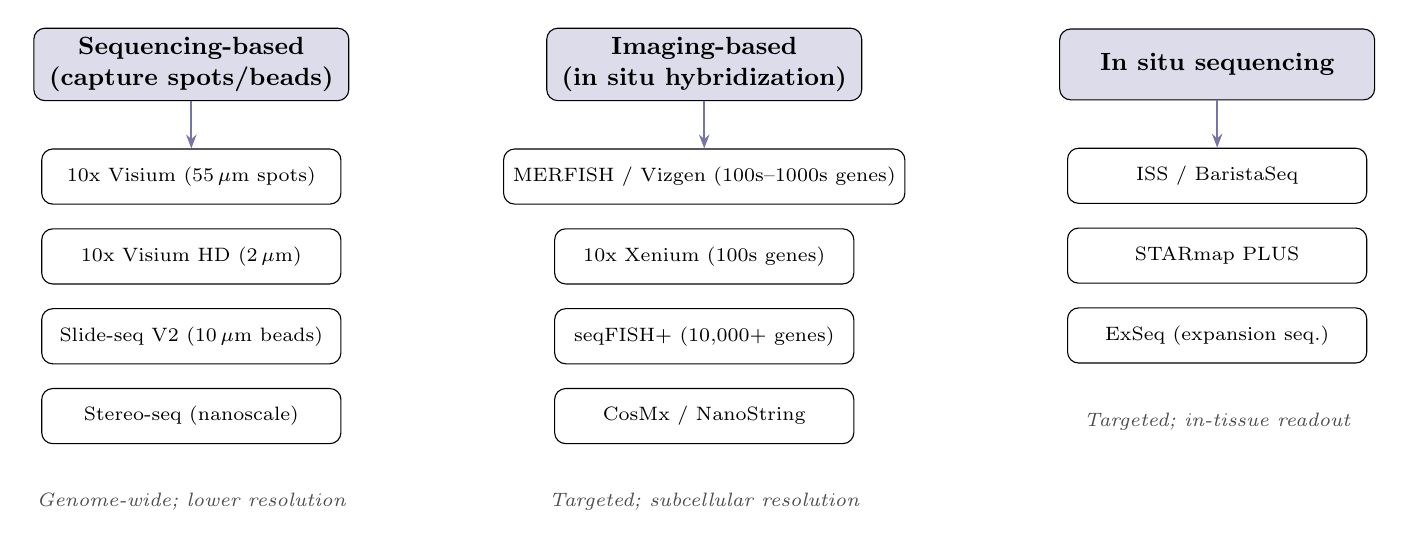
\begin{tikzpicture}[
  node distance=0.5cm and 1.0cm,
  every node/.style={font=\small},
  category/.style={draw, rounded corners, fill=MidnightBlue!15,
    minimum width=4.0cm, minimum height=0.9cm, align=center,
    font=\small\bfseries},
  platform/.style={draw, rounded corners, fill=white,
    minimum width=3.8cm, minimum height=0.7cm, align=center,
    font=\scriptsize},
  arrow/.style={-{Stealth[length=5pt]}, thick, MidnightBlue!60},
  label/.style={font=\scriptsize\itshape, text=gray!60!black},
]

% Categories
\node[category] (seq) {Sequencing-based\\(capture spots/beads)};
\node[category, right=2.5cm of seq] (img) {Imaging-based\\(in situ hybridization)};
\node[category, right=2.5cm of img] (iss) {In situ sequencing};

% Sequencing-based platforms
\node[platform, below=0.6cm of seq] (visium) {10x Visium (55\,$\mu$m spots)};
\node[platform, below=0.3cm of visium] (visiumhd) {10x Visium HD (2\,$\mu$m)};
\node[platform, below=0.3cm of visiumhd] (slideseq) {Slide-seq V2 (10\,$\mu$m beads)};
\node[platform, below=0.3cm of slideseq] (stereo) {Stereo-seq (nanoscale)};

% Imaging-based platforms
\node[platform, below=0.6cm of img] (merfish) {MERFISH / Vizgen (100s--1000s genes)};
\node[platform, below=0.3cm of merfish] (xenium) {10x Xenium (100s genes)};
\node[platform, below=0.3cm of xenium] (seqfish) {seqFISH+ (10,000+ genes)};
\node[platform, below=0.3cm of seqfish] (cosmx) {CosMx / NanoString};

% In situ sequencing
\node[platform, below=0.6cm of iss] (issplat) {ISS / BaristaSeq};
\node[platform, below=0.3cm of issplat] (starmap) {STARmap PLUS};
\node[platform, below=0.3cm of starmap] (exseq) {ExSeq (expansion seq.)};

% Arrows from categories to first platform
\draw[arrow] (seq.south) -- (visium.north);
\draw[arrow] (img.south) -- (merfish.north);
\draw[arrow] (iss.south) -- (issplat.north);

% Annotations at bottom
\node[label, below=0.5cm of stereo] {Genome-wide; lower resolution};
\node[label, below=0.5cm of cosmx] {Targeted; subcellular resolution};
\node[label, below=0.5cm of exseq] {Targeted; in-tissue readout};

\end{tikzpicture}
\caption{Overview of spatial transcriptomics technology categories. Sequencing-based
methods (left) capture RNA at spatially barcoded positions and sequence it
off-tissue. Imaging-based methods (center) visualize individual RNA molecules
in situ using fluorescent probes. In situ sequencing methods (right) perform
the sequencing reaction directly within the tissue section.}
\label{fig:spatial:overview}
\end{figure}


% ---------------------------------------------------------------------------
\subsection{Sequencing-Based Spatial Methods}
\label{sec:spatial:seqbased}

These methods capture RNA from intact tissue sections onto spatially barcoded
surfaces. The tissue is permeabilized, RNA molecules are captured by
underlying barcoded oligonucleotides, and the resulting cDNA is sequenced
off-tissue using standard Illumina platforms. The spatial barcode allows each
transcript to be mapped back to its location in the tissue.

\subsubsection{10x Visium}

The most widely adopted spatial transcriptomics platform:

\begin{protocolbox}[title={10x Visium Workflow}]
\begin{enumerate}[nosep]
  \item Mount a fresh-frozen or FFPE tissue section (10\,$\mu$m thick) onto a
    Visium capture slide.
  \item Stain and image the section (H\&E for fresh-frozen; immunofluorescence
    for FFPE).
  \item Permeabilize the tissue to release mRNA (fresh-frozen) or after probe
    hybridization (FFPE).
  \item mRNA binds to spatially barcoded oligo-dT probes printed on the slide
    surface.
  \item Reverse transcription incorporates the spatial barcode into cDNA.
  \item cDNA is collected, amplified, and sequenced on Illumina.
  \item Reads are mapped and demultiplexed by spatial barcode using
    \software{Space Ranger}.
\end{enumerate}
\end{protocolbox}

\textbf{Key specifications:}
\begin{itemize}[nosep]
  \item \textbf{Resolution:} 55\,$\mu$m diameter capture spots arranged in a
    hexagonal grid with 100\,$\mu$m center-to-center spacing. Each spot covers
    1--10 cells (depending on tissue and cell size).
  \item \textbf{Gene coverage:} Genome-wide (no panel required); typically
    $\sim$3,000--8,000 genes detected per spot.
  \item \textbf{Capture area:} 6.5 mm $\times$ 6.5 mm, containing $\sim$5,000
    spots.
  \item \textbf{Sequencing depth:} 50,000--100,000 reads per spot recommended.
  \item \textbf{Sample types:} Fresh-frozen and FFPE (with dedicated Visium
    for FFPE workflow using probe-based capture).
\end{itemize}

\begin{warningbox}
Visium spots are not single cells. Each 55\,$\mu$m spot typically contains
multiple cells, creating a mixture of cell types within each spot. Computational
deconvolution methods (see \cref{sec:spatial:deconv}) are needed to infer
cell type composition per spot.
\end{warningbox}

\subsubsection{10x Visium HD}

The next-generation Visium platform with dramatically improved resolution:

\begin{itemize}[nosep]
  \item \textbf{Resolution:} 2\,$\mu$m $\times$ 2\,$\mu$m barcoded squares,
    providing near-single-cell or subcellular resolution.
  \item \textbf{Binning:} Data can be analyzed at 2\,$\mu$m, 8\,$\mu$m, or
    16\,$\mu$m resolution by binning adjacent squares.
  \item \textbf{Gene coverage:} Genome-wide.
  \item \textbf{Continuous tiling:} No gaps between capture positions, unlike
    the original Visium.
  \item \textbf{Sample types:} FFPE tissues; fresh-frozen support was added
    subsequently.
  \item Analyzed with \software{Space Ranger} (HD mode).
\end{itemize}

\subsubsection{Slide-seq and Slide-seqV2}

\begin{itemize}[nosep]
  \item \textbf{Principle:} A dense monolayer of DNA-barcoded 10\,$\mu$m beads
    (``puck'') is used as the capture surface. Beads are decoded by sequential
    hybridization (\textit{Slide-seq}) or by sequencing (Slide-seqV2) to
    determine their spatial position.
  \item \textbf{Resolution:} 10\,$\mu$m (near single-cell for most tissues).
  \item \textbf{Gene detection:} Lower than Visium ($\sim$500--2,000 genes per
    bead), but higher spatial resolution.
  \item \textbf{Open-source:} Protocols and analysis tools are publicly
    available.
\end{itemize}

\subsubsection{Stereo-seq (BGI)}

\begin{itemize}[nosep]
  \item \textbf{Principle:} DNA nanoball (DNB)-based spatial barcoding on a
    patterned array. Achieves nanoscale resolution ($\sim$500\,nm spot size).
  \item \textbf{Capture area:} Up to full tissue sections (centimeter scale).
  \item \textbf{Resolution:} Subcellular ($\sim$0.5\,$\mu$m), binnable to any
    desired resolution.
  \item \textbf{Notable application:} Used to create the first spatially
    resolved transcriptomic atlas of an entire mouse embryo (MOSTA).
  \item \textbf{Gene coverage:} Genome-wide.
\end{itemize}

\subsubsection{Other Sequencing-Based Methods}

\begin{description}[style=nextline]
  \item[HDST (High-Definition Spatial Transcriptomics)] Uses 2\,$\mu$m
    barcoded wells. An early demonstration of high-resolution capture-based
    spatial transcriptomics.
  \item[Seq-Scope] Repurposes Illumina flow cells as spatial capture surfaces,
    achieving $\sim$0.5--1\,$\mu$m resolution with genome-wide gene coverage
    at very low cost per unit area.
\end{description}


\subsection{Imaging-Based Spatial Methods (In Situ Hybridization)}
\label{sec:spatial:imaging}

Imaging-based methods detect individual RNA molecules in intact tissue by
hybridizing fluorescent probes directly to transcripts. They achieve
subcellular resolution and can image specific panels of 100--10,000+ genes.

\subsubsection{MERFISH (Multiplexed Error-Robust FISH)}

Developed by the Zhuang lab (Harvard) and commercialized by Vizgen:

\begin{keyconcept}[title={How MERFISH Works}]
\begin{enumerate}[nosep]
  \item Design encoding probes for each target gene. Each gene is assigned a
    unique binary barcode (e.g., a 16-bit code using a modified Hamming
    distance error-correcting scheme).
  \item Hybridize all encoding probes simultaneously to the tissue.
  \item Perform multiple rounds of sequential imaging:
    \begin{itemize}[nosep]
      \item In each round, readout probes complementary to specific barcode
        positions bind and fluoresce.
      \item Image the tissue, record fluorescent spots.
      \item Strip the readout probes (photobleach or chemically remove).
      \item Repeat for the next round.
    \end{itemize}
  \item Each RNA molecule generates a pattern of ON/OFF signals across rounds,
    spelling out its binary barcode.
  \item Error correction (Hamming distance codes) allows identification and
    correction of single-bit errors, dramatically reducing false positives.
\end{enumerate}
\end{keyconcept}

\textbf{Key specifications:}
\begin{itemize}[nosep]
  \item \textbf{Gene panel:} 100--1,000+ genes (MERSCOPE platform from Vizgen
    supports panels of 140--1,000 genes; custom panels possible).
  \item \textbf{Resolution:} Single-molecule, subcellular
    ($\sim$100\,nm localization).
  \item \textbf{Throughput:} Millions of cells per tissue section.
  \item \textbf{Imaging time:} 12--48 hours per tissue section depending on
    panel size and area.
\end{itemize}

\subsubsection{seqFISH+}

\begin{itemize}[nosep]
  \item An extension of seqFISH that profiles $>$10,000 genes per cell.
  \item Uses sequential rounds of hybridization with pseudo-color barcoding
    (multiple fluorescent channels per round).
  \item Achieves transcriptome-scale imaging but at lower throughput than
    MERFISH due to the large number of imaging rounds required.
  \item Academic protocol; not commercially available as a turnkey system.
\end{itemize}

\subsubsection{10x Xenium}

The in situ platform from 10x Genomics:

\begin{itemize}[nosep]
  \item \textbf{Principle:} Padlock probe-based detection. Pairs of probes
    hybridize to target RNA; when correctly paired, they are ligated and
    amplified via rolling circle amplification (RCA), creating a bright
    fluorescent spot.
  \item \textbf{Gene panel:} Pre-designed panels (human brain, breast cancer,
    lung, immune, multi-tissue) covering 300--500 genes, plus custom panels
    up to 480 genes. Higher multiplex panels continue to be released.
  \item \textbf{Resolution:} Subcellular (detects individual transcripts within
    cells and can resolve nuclear vs.\ cytoplasmic localization).
  \item \textbf{Throughput:} Large tissue areas (full tissue sections);
    automated instrument with $\sim$24-hour run time per slide.
  \item \textbf{FFPE compatible:} Works with FFPE tissues, enabling retrospective
    spatial analysis of archival samples.
  \item \textbf{Integrated analysis:} Results can be directly overlaid with
    Visium data from adjacent sections for combined genome-wide + targeted
    spatial analysis.
\end{itemize}

\subsubsection{CosMx Spatial Molecular Imager (NanoString)}

\begin{itemize}[nosep]
  \item Probe-based in situ hybridization platform.
  \item Gene panels of 1,000--6,000 genes for RNA and 64--100 proteins
    simultaneously (multi-omic spatial profiling).
  \item Subcellular resolution; automated imaging system.
  \item Compatible with FFPE tissues.
  \item Multi-omic capability (RNA + protein in the same tissue section) is a
    key differentiator.
\end{itemize}

\subsubsection{FISH-Based Principles}

All imaging-based spatial methods rely on variations of fluorescence in situ
hybridization (FISH):

\begin{description}[style=nextline]
  \item[Single-molecule FISH (smFISH)] The foundational method: multiple
    fluorescent probes tile along a single RNA transcript, producing a
    diffraction-limited spot visible under a fluorescence microscope. Detects
    one gene per fluorescence channel (typically 3--5 genes per experiment).
  \item[Combinatorial barcoding] MERFISH and seqFISH assign each gene a
    binary barcode read out across multiple rounds of imaging. This
    exponentially scales the number of genes: $n$ rounds with error correction
    can encode thousands of genes.
  \item[Sequential hybridization] Probes are applied, imaged, removed, and
    replaced in successive rounds. Each round reveals a different subset of
    genes or barcode positions.
\end{description}


\subsection{In Situ Sequencing}
\label{sec:spatial:insitu}

In situ sequencing (ISS) methods perform the sequencing reaction directly
within the tissue, reading out short barcodes that identify each transcript.

\begin{description}[style=nextline]
  \item[ISS (In Situ Sequencing)] Padlock probes hybridize to target RNAs;
    gaps are filled and ligated to form circular DNA. Rolling circle
    amplification (RCA) creates dense DNA nanoballs that are sequenced in situ
    by sequencing-by-ligation. Typically reads 4--5 bases (sufficient for
    barcode identification).
  \item[BaristaSeq] An improved ISS method with higher efficiency gap-filling
    and sequencing-by-synthesis readout. Compatible with tissue clearing for
    3D spatial transcriptomics.
  \item[STARmap / STARmap PLUS] Uses SNAIL (specific amplification of nucleic
    acids via intramolecular ligation) probes for highly multiplexed in situ
    sequencing. STARmap PLUS scales to 1,000+ genes. Compatible with intact
    tissue (hydrogel-embedded) for volumetric 3D spatial transcriptomics.
  \item[ExSeq (Expansion Sequencing)] Combines expansion microscopy (physically
    enlarging the tissue by embedding in a swellable hydrogel) with in situ
    RNA sequencing. Achieves nanoscale resolution of RNA localization within
    subcellular compartments (dendrites, synapses).
\end{description}


% ---------------------------------------------------------------------------
\section{Comparison of Spatial Transcriptomics Platforms}
\label{sec:spatial:comparison}

\begin{table}[htbp]
\centering
\caption{Comprehensive comparison of spatial transcriptomics platforms.}
\label{tab:spatial:platforms}
\footnotesize
\begin{tabularx}{\textwidth}{lXXXXX}
\toprule
\textbf{Feature} & \textbf{Visium} & \textbf{Visium HD} & \textbf{MERFISH} & \textbf{Xenium} & \textbf{Stereo-seq} \\
\midrule
Category & Seq-based & Seq-based & Imaging & Imaging & Seq-based \\
Resolution & 55\,$\mu$m & 2\,$\mu$m & Subcellular & Subcellular & 0.5\,$\mu$m \\
Gene coverage & Genome-wide & Genome-wide & 100--1,000 & 300--500 & Genome-wide \\
Cells per section & $\sim$5,000 spots & $\sim$millions of bins & Millions & Millions & Millions \\
FFPE compatible & Yes (v2) & Yes & Limited & Yes & Yes \\
Instrument & None (slide) & None (slide) & MERSCOPE & Xenium Analyzer & STOmics \\
Run time & 1--2 days (wet lab) & 1--2 days (wet lab) & 12--48 h imaging & $\sim$24 h & 1--2 days \\
Analysis software & Space Ranger & Space Ranger & Vizgen MERSCOPE & Xenium Ranger/Explorer & STOmics tools \\
Cost per section & \$\$\$ & \$\$\$ & \$\$\$\$ & \$\$\$ & \$\$\$ \\
Best use case & Genome-wide discovery & High-res discovery & Targeted, subcellular & Clinical FFPE, targeted & Large-area mapping \\
\bottomrule
\end{tabularx}
\end{table}

\begin{table}[htbp]
\centering
\caption{Extended comparison including additional platforms.}
\label{tab:spatial:platforms_extended}
\footnotesize
\begin{tabularx}{\textwidth}{lXXXXX}
\toprule
\textbf{Feature} & \textbf{Slide-seqV2} & \textbf{seqFISH+} & \textbf{CosMx} & \textbf{STARmap PLUS} & \textbf{Seq-Scope} \\
\midrule
Category & Seq-based & Imaging & Imaging & In situ seq. & Seq-based \\
Resolution & 10\,$\mu$m & Subcellular & Subcellular & Subcellular & $\sim$0.6\,$\mu$m \\
Gene coverage & Genome-wide & 10,000+ & 1,000--6,000 & 1,000+ & Genome-wide \\
Multi-omic & No & No & RNA + protein & No & No \\
Commercial & No (academic) & No (academic) & Yes (NanoString) & No (academic) & No (academic) \\
3D capable & No & Limited & No & Yes & No \\
\bottomrule
\end{tabularx}
\end{table}

\begin{tipbox}
Choosing a spatial technology depends on your biological question:
\begin{itemize}[nosep]
  \item \textbf{Unbiased discovery (genome-wide):} Visium, Visium HD, or
    Stereo-seq.
  \item \textbf{Targeted subcellular resolution:} MERFISH (Vizgen), Xenium
    (10x), or CosMx (NanoString).
  \item \textbf{FFPE clinical samples:} Xenium, Visium FFPE, or CosMx.
  \item \textbf{Combined RNA + protein:} CosMx (NanoString).
  \item \textbf{3D spatial transcriptomics:} STARmap PLUS or ExSeq.
\end{itemize}
Many studies now combine a genome-wide method (e.g., Visium HD) with a targeted
imaging method (e.g., Xenium) on serial sections to get both breadth and
resolution.
\end{tipbox}


% ---------------------------------------------------------------------------
\section{Computational Analysis for Spatial Transcriptomics}
\label{sec:spatial:computation}

Spatial transcriptomics data requires specialized computational methods that
account for the spatial dimensions in addition to the gene expression matrix.

\subsection{Spot Deconvolution}
\label{sec:spatial:deconv}

For Visium and other methods where each measurement captures multiple cells,
deconvolution estimates the proportion of each cell type within each spatial
location by leveraging a single-cell RNA-seq reference:

\begin{description}[style=nextline]
  \item[\software{cell2location}] Bayesian model that estimates absolute cell
    type abundances per spot by decomposing the spatial expression profile into
    a mixture of reference scRNA-seq signatures. Provides uncertainty estimates
    and handles overdispersion. One of the most widely used and best-performing
    methods in benchmarks.
  \item[\software{RCTD} (Robust Cell Type Decomposition)] Part of the
    \software{spacexr} R package. Fits a weighted regression model to estimate
    cell type proportions. Fast and robust; handles platform-specific technical
    differences between spatial and scRNA-seq data.
  \item[\software{Tangram}] Deep learning-based method that maps scRNA-seq
    cells to spatial locations by learning an optimal alignment between the
    two modalities. Can operate at both spot (Visium) and single-cell (Xenium,
    MERFISH) resolution.
  \item[\software{SPOTlight}] Uses non-negative matrix factorization (NMF) to
    decompose Visium spots into cell type proportions.
  \item[\software{stereoscope}] Probabilistic method based on negative binomial
    distributions for deconvolving spatial spots.
\end{description}

\begin{keyconcept}[title={Why Deconvolution Needs a scRNA-seq Reference}]
Deconvolution is fundamentally a source-separation problem: given a mixture
signal (the spatial spot), determine the contributing sources (cell types).
This requires knowing what each source looks like in isolation, which comes
from a scRNA-seq reference of the same tissue. The quality of deconvolution
depends critically on the completeness and accuracy of the reference atlas.
Missing cell types in the reference will be missed in the spatial data.
\end{keyconcept}

\subsubsection{Mathematical Framework for Spot Deconvolution}
\label{subsec:spatial:deconv_math}

The central idea behind methods like \software{RCTD} and
\software{cell2location} is that the observed expression profile at each
spatial location is a mixture of cell-type-specific expression signatures.
Formally, for spot $s$ with observed gene expression vector $Y_s$ (a vector of
length $G$, one entry per gene), the linear mixture model is:
\begin{equation}
  \label{eq:spatial:deconv_linear}
  Y_s = \sum_{k=1}^{K} w_{sk} \cdot \mu_k + \epsilon_s
\end{equation}
where $K$ is the number of cell types in the reference, $\mu_k$ is the
reference expression profile (mean expression vector) for cell type $k$,
$w_{sk} \geq 0$ is the weight (proportion or abundance) of cell type $k$ in
spot $s$, and $\epsilon_s$ represents noise (technical and biological).

\begin{description}[style=nextline]
  \item[\software{RCTD} formulation] Models the observed counts at each spot
    as a weighted sum of cell-type profiles using a platform-corrected
    regression framework. The weights $w_{sk}$ are constrained to be
    non-negative and are estimated via maximum likelihood under a Poisson or
    negative binomial noise model. RCTD explicitly accounts for
    platform-specific effects (differences in capture efficiency and gene
    detection between the spatial and scRNA-seq platforms) by estimating
    platform-specific normalisation factors.
  \item[\software{cell2location} formulation] Uses a hierarchical Bayesian
    model where the expected expression at spot $s$ for gene $g$ is:
    \begin{equation}
      \label{eq:spatial:cell2loc}
      \mathbb{E}[Y_{sg}] = \sum_{k=1}^{K} w_{sk} \cdot g_{kg} \cdot y_s
    \end{equation}
    where $g_{kg}$ is the reference expression of gene $g$ in cell type $k$
    (estimated from the scRNA-seq data), $y_s$ is a spot-level scaling factor,
    and $w_{sk}$ represents the absolute number of cells of type $k$ at spot
    $s$. Bayesian inference (using variational inference in \software{Pyro})
    provides full posterior distributions over all parameters, yielding
    uncertainty estimates for cell type abundances---a key advantage for
    downstream hypothesis testing.
\end{description}

\begin{tipbox}
When choosing a deconvolution method, consider whether you need
\emph{proportions} (what fraction of each spot is cell type $k$?) or
\emph{absolute abundances} (how many cells of type $k$?).
\software{RCTD} estimates proportions by default; \software{cell2location}
estimates absolute abundances. For comparing cell type composition across spots,
proportions suffice. For estimating total cell counts (e.g., immune infiltration
density), absolute abundances are more informative.
\end{tipbox}

\subsection{Spatially Variable Gene Detection}

Identifying genes whose expression varies as a function of spatial location,
beyond what would be expected by chance:

\begin{description}[style=nextline]
  \item[\software{SpatialDE}] Gaussian process regression model that tests
    whether the spatial variance component of gene expression is significant.
    Identifies genes with spatial patterns (e.g., gradients, periodic patterns,
    hotspots) and classifies them by spatial pattern type.
  \item[\software{SPARK}] Spatial Pattern Recognition via Kernels. Tests for
    spatially variable expression using a generalized linear spatial model with
    multiple spatial kernel functions. More powerful than SpatialDE for
    detecting diverse spatial patterns.
  \item[\software{Moran's I}] A classical spatial autocorrelation statistic
    applied to gene expression. Positive Moran's I indicates spatial clustering;
    negative values indicate spatial dispersion. Simple and fast; implemented in
    Squidpy and Giotto.
  \item[\software{nnSVG}] Nearest-neighbor Gaussian process model for
    identifying spatially variable genes. Scales better than SpatialDE to
    high-resolution platforms like Visium HD.
\end{description}

\subsubsection{Moran's I: Spatial Autocorrelation in Detail}
\label{subsec:spatial:morans_i}

Moran's $I$ is the most widely used statistic for quantifying spatial
autocorrelation of gene expression. For a gene with expression values
$x_1, x_2, \ldots, x_n$ measured at $n$ spatial locations, Moran's $I$ is
defined as:
\begin{equation}
  \label{eq:spatial:morans_i}
  I = \frac{n}{\sum_{i} \sum_{j} w_{ij}}
    \cdot
    \frac{\sum_{i} \sum_{j} w_{ij}\,(x_i - \bar{x})(x_j - \bar{x})}
         {\sum_{i} (x_i - \bar{x})^2}
\end{equation}
where $\bar{x} = \frac{1}{n}\sum_i x_i$ is the global mean expression,
$w_{ij}$ is the spatial weight between locations $i$ and $j$ (typically 1 if
$i$ and $j$ are neighbors and 0 otherwise, or a distance-decay function), and
the double sum runs over all pairs of locations.

\textbf{Interpretation:}
\begin{itemize}[nosep]
  \item $I > 0$: \textbf{Positive spatial autocorrelation} (clustering).
    Nearby locations tend to have similar expression values. Values close to
    +1 indicate strong spatial clustering.
  \item $I \approx 0$: \textbf{No spatial autocorrelation} (random spatial
    pattern). Expression is distributed independently of spatial position.
  \item $I < 0$: \textbf{Negative spatial autocorrelation} (dispersion).
    Nearby locations tend to have dissimilar expression values, forming a
    checkerboard-like pattern. This is rare for gene expression data.
\end{itemize}

The expected value under the null hypothesis of spatial randomness is
$\mathbb{E}[I] = -1/(n-1)$, which approaches zero for large $n$.
Statistical significance is assessed either analytically (under normality
assumptions) or by a permutation test that randomly shuffles expression values
across locations and recomputes $I$ to build a null distribution.

\begin{keyconcept}[title={Choosing the Spatial Weight Matrix}]
The spatial weight matrix $W = \{w_{ij}\}$ encodes the definition of ``spatial
proximity'' and critically affects the results:
\begin{itemize}[nosep]
  \item \textbf{Binary adjacency:} $w_{ij} = 1$ if spots $i$ and $j$ are direct
    neighbors (e.g., adjacent hexagons in Visium). Simple and fast.
  \item \textbf{KNN graph:} $w_{ij} = 1$ for the $k$ nearest neighbors of each
    spot. Robust when spot density varies across the tissue.
  \item \textbf{Distance decay:} $w_{ij} = f(d_{ij})$, e.g., Gaussian kernel
    $\exp(-d_{ij}^2 / 2h^2)$ or inverse distance. Captures longer-range spatial
    correlations (e.g., paracrine signaling gradients).
\end{itemize}
In \software{Squidpy}, the default spatial neighbors graph uses Delaunay
triangulation or KNN, and Moran's $I$ is computed via
\texttt{sq.gr.spatial\_autocorr(adata, mode="moran")}.
\end{keyconcept}

\subsection{Spatial Domain Identification}

Identifying tissue regions (``spatial domains'') with coherent gene expression
programs---analogous to clustering in scRNA-seq but incorporating spatial
proximity:

\begin{description}[style=nextline]
  \item[\software{BayesSpace}] Bayesian approach that models spatial
    transcriptomics data on a lattice graph, encouraging neighboring spots to
    belong to the same cluster. Produces spatially smooth domain assignments.
    Supports Visium and Slide-seq data.
  \item[\software{SpaGCN}] Uses a graph convolutional network that integrates
    gene expression, spatial coordinates, and histology image features to
    identify spatial domains. Learns optimal representations that combine
    molecular and morphological information.
  \item[\software{STAGATE}] Graph attention auto-encoder that identifies spatial
    domains by learning a latent representation that incorporates spatial
    neighbor information via attention mechanisms.
  \item[\software{BANKSY}] Builds a neighborhood expression matrix that
    combines each spot's own expression with the average expression of its
    spatial neighbors. Standard clustering on this augmented matrix produces
    spatially coherent domains without specialized spatial algorithms.
\end{description}

\subsection{Integration with scRNA-seq}

Integrating spatial transcriptomics data with scRNA-seq enables cell type
mapping and enhances the resolution of spatial data:

\begin{itemize}[nosep]
  \item \textbf{Deconvolution} (see \cref{sec:spatial:deconv}): Infer cell type
    proportions at each spatial location.
  \item \textbf{Imputation:} Predict the expression of unmeasured genes in
    targeted spatial assays (MERFISH, Xenium) by transferring information from
    a genome-wide scRNA-seq reference. Tools: \software{Tangram},
    \software{gimVI} (scvi-tools), \software{novoSpaRc}.
  \item \textbf{Label transfer:} Project cell type annotations from scRNA-seq
    reference onto spatial spots using anchor-based integration (Seurat) or
    probabilistic assignment (cell2location, Tangram).
\end{itemize}

\subsection{Ligand--Receptor Analysis in Spatial Context}

Spatial data enables direct testing of cell--cell communication hypotheses
because the physical proximity of sender and receiver cells is known:

\begin{description}[style=nextline]
  \item[\software{stLearn}] Combines spatial distance with ligand--receptor
    co-expression to identify spatially constrained cell--cell interactions.
    Only considers interactions between cell types that are physically adjacent.
  \item[\software{COMMOT}] Uses optimal transport theory to model the spatial
    flow of signaling molecules from sender to receiver locations. Produces
    spatial vector fields showing the direction and magnitude of each signaling
    pathway.
  \item[\software{MISTy}] Multi-view framework that models gene expression at
    each spot as a function of its intrinsic state, its immediate neighborhood
    (juxtacrine signaling), and its broader tissue context (paracrine
    signaling). Identifies the spatial scale at which different pathways
    operate.
  \item[\software{Squidpy}] General-purpose spatial analysis framework (see
    below) that includes neighborhood enrichment analysis and ligand--receptor
    co-occurrence testing.
\end{description}

\subsubsection{Ligand--Receptor Communication Scoring: Mathematical Framework}
\label{subsec:spatial:lr_scoring}

Spatial ligand--receptor analysis quantifies the probability or strength of
signaling between spatially proximal cell populations. The \software{CellChat}
framework (originally developed for scRNA-seq) and the spatial extension
\software{COMMOT} both model communication probability based on the expression
levels of ligand and receptor genes, weighted by spatial proximity.

\textbf{CellChat communication probability.} For a ligand--receptor pair
$(L, R)$ between sender cell type $A$ and receiver cell type $B$, CellChat
computes a communication score based on the law of mass action:
\begin{equation}
  \label{eq:spatial:cellchat_prob}
  P_{L,R}^{A \to B} = \frac{\bar{x}_L^A \cdot \bar{x}_R^B}
    {K_h + \bar{x}_L^A \cdot \bar{x}_R^B}
\end{equation}
where $\bar{x}_L^A$ is the average expression of ligand $L$ in sender
population $A$, $\bar{x}_R^B$ is the average expression of receptor $R$ in
receiver population $B$, and $K_h$ is a half-saturation constant (Hill function
parameterization) that prevents extreme scores when expression is very high.
For multi-subunit receptors (e.g., heterodimeric complexes), the receptor
expression is taken as the geometric mean of subunit expression levels.

\textbf{Spatial weighting in COMMOT.} The \software{COMMOT} framework extends
ligand--receptor scoring to spatial transcriptomics by incorporating spatial
distance as a modulating factor. For each pair of spatial locations $(i, j)$
with distance $d_{ij}$, the spatial communication score is:
\begin{equation}
  \label{eq:spatial:commot_score}
  S_{ij}^{L,R} = x_{L,i} \cdot x_{R,j} \cdot K(d_{ij})
\end{equation}
where $x_{L,i}$ is the expression of ligand $L$ at location $i$, $x_{R,j}$ is
the expression of receptor $R$ at location $j$, and $K(d_{ij})$ is a spatial
kernel function that down-weights interactions at greater distances. Common
choices include:
\begin{itemize}[nosep]
  \item \textbf{Cutoff kernel:} $K(d) = \mathbf{1}[d \leq d_{\max}]$ (binary;
    interactions only within a maximum range).
  \item \textbf{Gaussian kernel:} $K(d) = \exp(-d^2 / 2\sigma^2)$ (smooth
    decay with characteristic scale $\sigma$).
\end{itemize}

\software{COMMOT} uses optimal transport theory to aggregate these pairwise
scores into \textbf{spatial communication vector fields}, showing the net
direction and magnitude of signaling flow for each pathway across the tissue.
These vector fields can reveal directional signaling patterns such as morphogen
gradients or immune cell recruitment.

\begin{warningbox}
Ligand--receptor scoring in spatial transcriptomics assumes that mRNA expression
is a reasonable proxy for protein abundance and secretion. This is not always
true: post-transcriptional regulation, protein half-life, and secretion
dynamics can decouple mRNA and protein levels. Spatial proteomics data (e.g.,
from CosMx or CODEX) can provide complementary validation for key signaling
interactions identified by transcriptomic methods.
\end{warningbox}

\subsection{Data Visualization and Analysis Frameworks}

\begin{description}[style=nextline]
  \item[\software{Squidpy}] Python package for spatial omics analysis built on
    top of Scanpy/AnnData. Provides image processing (segmentation, feature
    extraction), graph construction (spatial neighbors), spatial statistics
    (Moran's I, co-occurrence, centrality scores), and interactive
    visualization. The primary Python framework for spatial transcriptomics.
  \item[\software{Giotto}] R and Python package providing a comprehensive suite
    for spatial data analysis: preprocessing, spatial network construction,
    spatial gene detection, domain identification, cell--cell interaction, and
    visualization with interactive viewers.
  \item[\software{Seurat} (spatial module)] Seurat v5 includes native support
    for spatial data (Visium, Xenium, MERFISH, Slide-seq). Functions for
    spatial feature plots, integration with scRNA-seq, and spatial
    dimensionality reduction.
  \item[\software{Voyager}] R/Bioconductor package implementing spatial
    statistics methods (variograms, correlograms, Moran's I, Geary's C) for
    spatial transcriptomics, built on the SpatialFeatureExperiment data
    structure.
  \item[\software{napari} + \software{spatialdata}] Python imaging viewer
    (napari) combined with the spatialdata framework for multi-modal spatial
    data handling (images, coordinates, annotations, expression). Enables
    interactive exploration of spatial datasets.
\end{description}


% ---------------------------------------------------------------------------
\section{Tissue Handling and Sample Preparation}
\label{sec:spatial:tissue}

Spatial transcriptomics requires careful tissue preparation---often more
demanding than standard sequencing experiments because tissue morphology must
be preserved.

\subsection{Tissue Sectioning}

\begin{itemize}[nosep]
  \item \textbf{Fresh-frozen (FF):} Tissue is flash-frozen in OCT compound
    (optimal cutting temperature) or isopentane. Sectioned at 10\,$\mu$m on a
    cryostat. Best RNA quality but limited long-term storage.
  \item \textbf{FFPE:} Formalin-fixed, paraffin-embedded. Sectioned at
    5--10\,$\mu$m on a microtome. RNA is crosslinked and fragmented but
    preserved indefinitely. Compatible with Visium FFPE, Xenium, CosMx.
  \item \textbf{Section quality:} Sections must be uniform in thickness,
    wrinkle-free, and fully adherent to the capture area. Tissue folds,
    tears, or bubbles create artifacts in spatial data.
\end{itemize}

\subsection{Permeabilization Optimization}

For sequencing-based methods (Visium), the tissue must be permeabilized to
release mRNA while keeping it localized above its capture spot.

\begin{protocolbox}[title={Visium Permeabilization Optimization}]
A tissue optimization (TO) experiment is performed before the main experiment:
\begin{enumerate}[nosep]
  \item Mount serial sections on a Visium TO slide.
  \item Permeabilize each section for a different duration (e.g., 3, 6, 12, 18,
    24, 30 minutes).
  \item Perform reverse transcription with fluorescent nucleotides.
  \item Image the fluorescent cDNA footprint under a microscope.
  \item Select the permeabilization time that maximizes signal (cDNA
    fluorescence) while maintaining spatial resolution (sharp edges, no
    lateral diffusion).
\end{enumerate}
Typical optimal permeabilization time: 6--18 minutes for most tissues, but
varies widely (e.g., brain requires less, skeletal muscle requires more).
\end{protocolbox}

\begin{warningbox}
Over-permeabilization causes RNA to diffuse laterally, blurring spatial
resolution. Under-permeabilization results in poor RNA capture. Each tissue
type requires its own optimization. Do not skip the tissue optimization step.
\end{warningbox}

\subsection{Imaging}

\begin{itemize}[nosep]
  \item \textbf{H\&E staining:} Standard histological stain for tissue
    morphology. Used with fresh-frozen Visium. The H\&E image is registered to
    the spatial gene expression data, allowing correlation of transcriptomic
    patterns with morphological features.
  \item \textbf{Immunofluorescence (IF):} Antibody-based staining for specific
    proteins. Used with FFPE Visium and Xenium. Provides protein-level
    information that complements the transcriptomic data.
  \item \textbf{Cell segmentation:} For imaging-based methods, individual cells
    must be segmented from the tissue image. Methods include DAPI-based nuclear
    segmentation (watershed, Cellpose, StarDist) and membrane staining
    (phalloidin, WGA). Accurate segmentation is critical for assigning
    transcripts to individual cells.
\end{itemize}


% ---------------------------------------------------------------------------
\section{Emerging Directions: Spatial Multi-Omics}
\label{sec:spatial:emerging}

\subsection{Spatial Epigenomics}

\begin{description}[style=nextline]
  \item[Spatial ATAC-seq] Methods such as spatial-ATAC-seq and
    Spatial-CUT\&Tag map chromatin accessibility and histone modifications
    in tissue sections. These reveal spatially resolved regulatory landscapes
    (enhancer usage, TF binding) that complement spatial gene expression.
  \item[10x Visium + ATAC] Emerging protocols from 10x Genomics that combine
    gene expression and chromatin accessibility on the same Visium slide.
\end{description}

\subsection{Spatial Proteomics}

\begin{description}[style=nextline]
  \item[CODEX (CO-Detection by indEXing)] Iterative antibody staining and
    imaging that profiles 40--60 proteins at single-cell resolution in intact
    tissues. Uses DNA-conjugated antibodies and fluorescent reporters that
    are sequentially activated and quenched.
  \item[MIBI-TOF (Multiplexed Ion Beam Imaging)] Uses metal-conjugated
    antibodies and time-of-flight mass spectrometry for highly multiplexed
    protein imaging ($>$40 markers).
  \item[CosMx multi-omic:] Simultaneous RNA and protein detection on the same
    tissue section (see above).
\end{description}

\subsection{Spatial Multi-Omic Integration}

The frontier of spatial biology is measuring multiple molecular layers
(transcriptome, epigenome, proteome, metabolome) in the same tissue section
or in serial sections from the same block:

\begin{itemize}[nosep]
  \item Serial section approaches: alternate sections for different assays
    (e.g., Visium + Xenium + CODEX on serial 10\,$\mu$m sections).
  \item Same-section multi-omics: CosMx (RNA + protein), Visium + IF, and
    emerging combined ATAC + RNA spatial methods.
  \item Computational integration: Tools such as \software{MEFISTO} (multi-omic
    factor analysis in space and time) and \software{MOFA+} enable joint
    analysis of spatial multi-omic datasets.
\end{itemize}


% ---------------------------------------------------------------------------
\section{Snakemake Workflow for Spatial Transcriptomics}
\label{sec:spatial:snakemake}

\begin{lstlisting}[language=Python, caption={Snakemake workflow for 10x Visium
spatial transcriptomics analysis.}, label={lst:spatial:snakemake}]
# Snakefile for Spatial Transcriptomics (10x Visium)
# ====================================================
# Pipeline: Space Ranger -> Squidpy / Scanpy analysis

import pandas as pd

configfile: "config/config.yaml"

samples = pd.read_csv(config["samples"], sep="\t")
SAMPLES = samples["sample"].tolist()

REFERENCE = config["spaceranger_ref"]

rule all:
    input:
        expand("results/spaceranger/{sample}/outs/"
               "filtered_feature_bc_matrix.h5",
               sample=SAMPLES),
        "results/squidpy/spatial_analysis.h5ad",
        "results/squidpy/spatial_domains.pdf",
        "results/deconvolution/cell2location_results.h5ad"

rule spaceranger_count:
    input:
        fastqs="data/raw/{sample}/",
        image="data/images/{sample}.tif",
        reference=REFERENCE
    output:
        h5="results/spaceranger/{sample}/outs/"
           "filtered_feature_bc_matrix.h5",
        spatial="results/spaceranger/{sample}/outs/spatial/",
        web="results/spaceranger/{sample}/outs/"
            "web_summary.html"
    threads: 12
    resources:
        mem_mb=64000
    params:
        outdir="results/spaceranger/{sample}",
        slide=lambda wc: samples.loc[
            samples["sample"] == wc.sample,
            "slide_serial"].iloc[0],
        area=lambda wc: samples.loc[
            samples["sample"] == wc.sample,
            "capture_area"].iloc[0]
    shell:
        """
        spaceranger count \
          --id={wildcards.sample} \
          --transcriptome={input.reference} \
          --fastqs={input.fastqs} \
          --image={input.image} \
          --slide={params.slide} \
          --area={params.area} \
          --localcores={threads} \
          --localmem=60 \
          --output-dir={params.outdir}
        """

rule squidpy_analysis:
    input:
        h5_files=expand(
            "results/spaceranger/{sample}/outs/"
            "filtered_feature_bc_matrix.h5",
            sample=SAMPLES),
        spatial_dirs=expand(
            "results/spaceranger/{sample}/outs/spatial/",
            sample=SAMPLES)
    output:
        h5ad="results/squidpy/spatial_analysis.h5ad",
        domains="results/squidpy/spatial_domains.pdf",
        svg_genes="results/squidpy/spatially_variable_genes.csv",
        co_occur="results/squidpy/co_occurrence.pdf"
    conda: "envs/squidpy.yaml"
    script:
        "scripts/run_squidpy.py"

rule cell2location:
    input:
        spatial="results/squidpy/spatial_analysis.h5ad",
        sc_ref=config["scrna_reference"]
    output:
        results="results/deconvolution/"
                "cell2location_results.h5ad",
        plots="results/deconvolution/"
              "cell_type_maps.pdf"
    resources:
        mem_mb=32000
    conda: "envs/cell2location.yaml"
    script:
        "scripts/run_cell2location.py"

rule spatial_communication:
    input:
        h5ad="results/squidpy/spatial_analysis.h5ad"
    output:
        commot="results/communication/"
               "spatial_signaling.h5ad",
        plots="results/communication/"
              "signaling_vectors.pdf"
    conda: "envs/commot.yaml"
    script:
        "scripts/run_commot.py"
\end{lstlisting}


% ---------------------------------------------------------------------------
\section{Nextflow Workflow for Spatial Transcriptomics}
\label{sec:spatial:nextflow}

\begin{lstlisting}[language=Java, caption={Nextflow DSL2 workflow for 10x
Visium spatial transcriptomics analysis.},
label={lst:spatial:nextflow}]
#!/usr/bin/env nextflow
// Spatial Transcriptomics Pipeline (Nextflow DSL2)
// ==================================================
// Pipeline: Space Ranger -> Squidpy -> cell2location

nextflow.enable.dsl = 2

params.sample_sheet = "config/samples.tsv"
params.reference    = "resources/refdata-gex-GRCh38-2024-A"
params.scrna_ref    = "resources/scrna_reference.h5ad"
params.outdir       = "results"

log.info """
==========================================
 Spatial Transcriptomics Pipeline
==========================================
 sample_sheet : ${params.sample_sheet}
 reference    : ${params.reference}
 scRNA ref    : ${params.scrna_ref}
 outdir       : ${params.outdir}
==========================================
"""

// Parse sample sheet
Channel
    .fromPath(params.sample_sheet)
    .splitCsv(header: true, sep: '\t')
    .map { row ->
        tuple(
            row.sample,
            file(row.fastq_dir),
            file(row.image),
            row.slide_serial,
            row.capture_area
        )
    }
    .set { samples_ch }

process SPACERANGER_COUNT {
    tag "$sample_id"
    publishDir "${params.outdir}/spaceranger/${sample_id}",
        mode: 'copy'
    cpus 12
    memory '64 GB'

    input:
    tuple val(sample_id), path(fastqs), path(image),
          val(slide), val(area)
    path(reference)

    output:
    tuple val(sample_id),
        path("outs/filtered_feature_bc_matrix.h5"),
        path("outs/spatial/"),
        emit: counts
    path("outs/web_summary.html"), emit: web_summary

    script:
    """
    spaceranger count \
      --id=${sample_id} \
      --transcriptome=${reference} \
      --fastqs=${fastqs} \
      --image=${image} \
      --slide=${slide} \
      --area=${area} \
      --localcores=${task.cpus} \
      --localmem=60
    """
}

process SQUIDPY_ANALYSIS {
    publishDir "${params.outdir}/squidpy", mode: 'copy'
    cpus 4
    memory '32 GB'

    input:
    path(h5_files)
    path(spatial_dirs)

    output:
    path("spatial_analysis.h5ad"),          emit: h5ad
    path("spatial_domains.pdf"),            emit: domains
    path("spatially_variable_genes.csv"),   emit: svg
    path("co_occurrence.pdf"),              emit: co_occur

    script:
    """
    python ${projectDir}/bin/run_squidpy.py \
      --input_h5 ${h5_files} \
      --spatial_dirs ${spatial_dirs} \
      --outdir .
    """
}

process CELL2LOCATION {
    publishDir "${params.outdir}/deconvolution", mode: 'copy'
    memory '32 GB'
    accelerator 1

    input:
    path(spatial_h5ad)
    path(scrna_ref)

    output:
    path("cell2location_results.h5ad"), emit: results
    path("cell_type_maps.pdf"),         emit: plots

    script:
    """
    python ${projectDir}/bin/run_cell2location.py \
      --spatial ${spatial_h5ad} \
      --sc_reference ${scrna_ref} \
      --outdir .
    """
}

process SPATIAL_COMMUNICATION {
    publishDir "${params.outdir}/communication", mode: 'copy'
    memory '16 GB'

    input:
    path(spatial_h5ad)

    output:
    path("spatial_signaling.h5ad"),  emit: results
    path("signaling_vectors.pdf"),   emit: plots

    script:
    """
    python ${projectDir}/bin/run_commot.py \
      --input ${spatial_h5ad} \
      --outdir .
    """
}

workflow {
    reference = Channel.fromPath(params.reference)

    // Space Ranger quantification
    SPACERANGER_COUNT(samples_ch, reference.collect())

    // Collect all samples for joint analysis
    SQUIDPY_ANALYSIS(
        SPACERANGER_COUNT.out.counts
            .map { it[1] }.collect(),
        SPACERANGER_COUNT.out.counts
            .map { it[2] }.collect()
    )

    // Cell type deconvolution
    CELL2LOCATION(
        SQUIDPY_ANALYSIS.out.h5ad,
        Channel.fromPath(params.scrna_ref)
    )

    // Spatial communication
    SPATIAL_COMMUNICATION(
        SQUIDPY_ANALYSIS.out.h5ad
    )
}
\end{lstlisting}

\begin{tipbox}
For production spatial transcriptomics analysis, the \software{nf-core/spatialtranscriptomics}
pipeline provides a Nextflow workflow supporting Space Ranger, quality control,
normalization, clustering, and basic spatial analysis with standardized outputs.
\end{tipbox}


% ---------------------------------------------------------------------------
\section{Practical Experimental Design Considerations}
\label{sec:spatial:design}

\subsection{Choosing the Right Technology}

\begin{itemize}[nosep]
  \item \textbf{Discovery vs.\ hypothesis-driven:} If you need genome-wide
    unbiased discovery, use a sequencing-based method (Visium, Visium HD,
    Stereo-seq). If you have a defined gene panel, imaging-based methods
    (MERFISH, Xenium) provide higher resolution and single-cell quantification.
  \item \textbf{Sample type:} FFPE samples have the widest compatibility
    (Visium FFPE, Xenium, CosMx). Fresh-frozen tissue generally yields better
    RNA quality for sequencing-based methods.
  \item \textbf{Resolution requirements:} If single-cell resolution is essential,
    use imaging-based methods or Visium HD. Standard Visium (55\,$\mu$m)
    requires computational deconvolution for cell type analysis.
  \item \textbf{Throughput:} For large cohorts (tens to hundreds of samples),
    consider the cost per section and instrument availability. Visium slides
    are relatively straightforward; imaging instruments have limited throughput
    (one section per $\sim$24 hours).
\end{itemize}

\subsection{Replication and Sample Size}

\begin{itemize}[nosep]
  \item Biological replicates (n $\geq$ 3 per condition) are needed for
    statistical testing of spatial gene expression differences.
  \item Technical replicates (serial sections from the same block) assess
    within-sample variability.
  \item Consider tissue heterogeneity: one section may not represent the entire
    organ. Multiple sections from different regions may be needed.
\end{itemize}

\subsection{Combining Spatial and Single-Cell Data}

\begin{protocolbox}[title={Recommended Multi-Modal Experimental Design}]
For comprehensive tissue profiling, a combined approach is often optimal:
\begin{enumerate}[nosep]
  \item \textbf{scRNA-seq:} Generate a reference atlas of cell types from
    dissociated tissue (10x Chromium, 5,000--10,000 cells per sample, n $\geq$ 3).
  \item \textbf{Spatial transcriptomics (genome-wide):} Profile serial sections
    with Visium or Visium HD for unbiased spatial gene expression mapping.
  \item \textbf{Spatial transcriptomics (targeted):} Profile adjacent sections
    with Xenium or MERFISH for single-cell resolution of key pathways.
  \item \textbf{Integration:} Use cell2location or Tangram to project scRNA-seq
    cell types onto spatial data; impute unmeasured genes in targeted data.
\end{enumerate}
This multi-modal approach provides genome-wide coverage (Visium), single-cell
resolution (Xenium), and a comprehensive cell type reference (scRNA-seq).
\end{protocolbox}


% ---------------------------------------------------------------------------
\section{Chapter Summary}
\label{sec:spatial:summary}

Spatial transcriptomics represents one of the most exciting frontiers in
genomics, bridging the gap between molecular profiling and tissue biology. In
this chapter we covered:

\begin{itemize}[nosep]
  \item Why spatial context matters: tissue architecture, cell neighborhoods,
    gradients, and the limitations of dissociation-based methods.
  \item Sequencing-based spatial methods: 10x Visium (55\,$\mu$m spots), Visium HD
    (2\,$\mu$m), Slide-seqV2 (10\,$\mu$m beads), Stereo-seq (nanoscale), and
    Seq-Scope.
  \item Imaging-based spatial methods: MERFISH (Vizgen), seqFISH+, 10x Xenium,
    and CosMx (NanoString), including the principles of combinatorial barcoding
    and sequential hybridization.
  \item In situ sequencing methods: ISS, BaristaSeq, STARmap PLUS, and ExSeq.
  \item Comprehensive platform comparisons covering resolution, gene coverage,
    throughput, and cost.
  \item Computational analysis: spot deconvolution (cell2location, RCTD,
    Tangram), spatially variable gene detection (SpatialDE, SPARK, Moran's I),
    spatial domain identification (BayesSpace, SpaGCN, STAGATE), scRNA-seq
    integration, and ligand--receptor analysis in spatial context (stLearn,
    COMMOT, MISTy).
  \item Visualization and analysis frameworks: Squidpy, Giotto, Seurat spatial
    module, Voyager.
  \item Tissue handling: sectioning (FF and FFPE), permeabilization
    optimization, imaging, and cell segmentation.
  \item Emerging directions: spatial ATAC-seq, spatial proteomics (CODEX,
    MIBI-TOF), and multi-omic spatial integration.
  \item Practical workflows in both Snakemake and Nextflow for Visium analysis.
\end{itemize}

Spatial transcriptomics, combined with the single-cell methods described in
\cref{ch:scrnaseq} and the bulk approaches in \cref{ch:rnaseq}, provides a
complete toolkit for transcriptomic analysis at every scale---from
population-level averages to individual molecules in their native tissue
context.


% Part V: Epigenomics and Chromatin
\part{Epigenomics: Beyond the Sequence}
\chapter{DNA Methylation Sequencing}
\label{ch:methylation}

\begin{sourcebox}
Bisulfite-aware alignment is anchored by the Bismark method paper \cite{krueger2011}. Bisulfite conversion generally conflates 5mC and 5hmC; claims of modification-specific detection must name the chemistry, model, controls, and validation standard.
\end{sourcebox}

\begin{keyconcept}
DNA methylation is a fundamental epigenetic modification in which a methyl group ($-\text{CH}_3$) is covalently added to the 5-carbon position of cytosine, forming \textbf{5-methylcytosine (5mC)}. This modification occurs predominantly at CpG dinucleotides in mammals and plays critical roles in gene silencing, genomic imprinting, X-chromosome inactivation, and cellular differentiation. Aberrant methylation patterns are hallmarks of cancer and other diseases. Multiple sequencing-based approaches---from bisulfite sequencing to enzymatic methods to direct nanopore detection---allow researchers to map methylation at single-base resolution across entire genomes.
\end{keyconcept}

%% ============================================================
\section{What Is DNA Methylation?}
\label{sec:methylation:what}

\subsection{5-Methylcytosine and CpG Dinucleotides}
\label{subsec:methylation:5mc}

In mammalian genomes, DNA methylation occurs almost exclusively at \textbf{CpG dinucleotides}---sites where a cytosine is immediately followed by a guanine on the same strand (written as 5$'$-CG-3$'$; the ``p'' denotes the phosphodiester bond). The methyl group is added to the 5-carbon of the cytosine ring by enzymes called \textbf{DNA methyltransferases (DNMTs)}:

\begin{itemize}[itemsep=2pt]
  \item \textbf{DNMT1} (maintenance methyltransferase): copies the methylation pattern from the parental strand to the newly synthesized daughter strand during DNA replication, ensuring epigenetic inheritance.
  \item \textbf{DNMT3A} and \textbf{DNMT3B} (de novo methyltransferases): establish new methylation patterns during embryonic development and cell differentiation.
  \item \textbf{DNMT3L}: a catalytically inactive family member that stimulates DNMT3A/3B activity.
\end{itemize}

Approximately 70--80\% of all CpG dinucleotides in the human genome are methylated. The remaining unmethylated CpGs are concentrated in specific genomic regions called \textbf{CpG islands (CGIs)}.

\subsection{CpG Islands}
\label{subsec:methylation:cpg-islands}

CpG islands are defined as regions of at least 200\basepair{} with a GC content $\geq$ 50\% and an observed-to-expected CpG ratio $\geq$ 0.6. The human genome contains approximately 28,000 CpG islands, of which roughly 60--70\% overlap with gene promoters. In normal somatic cells, most CpG islands at gene promoters are unmethylated, allowing gene expression. Methylation of a promoter CpG island typically leads to transcriptional silencing.

\begin{keyconcept}[title={CpG Depletion in the Genome}]
The CpG dinucleotide is under-represented in mammalian genomes (occurring at roughly 20\% of the expected frequency), because methylated cytosines spontaneously deaminate to thymine. Over evolutionary time, this mutation pressure has depleted CpGs from most of the genome. CpG islands have been maintained by purifying selection because they serve essential regulatory functions.
\end{keyconcept}

In addition to CpG islands, important regulatory methylation occurs at:
\begin{itemize}[itemsep=2pt]
  \item \textbf{CpG island shores}: regions 0--2\kilobase{} flanking CpG islands, where tissue-specific differential methylation is particularly common.
  \item \textbf{CpG island shelves}: regions 2--4\kilobase{} from CpG islands.
  \item \textbf{Enhancers and gene bodies}: intragenic methylation correlates with active transcription, and enhancer methylation is often inversely correlated with enhancer activity.
\end{itemize}

\subsection{Biological Roles of DNA Methylation}
\label{subsec:methylation:biological-roles}

DNA methylation participates in numerous biological processes:

\begin{enumerate}[itemsep=3pt]
  \item \textbf{Gene silencing:} Methylation at promoter CpG islands recruits methyl-binding domain (MBD) proteins, which in turn recruit histone deacetylases and chromatin remodelers to compact chromatin and silence transcription.
  \item \textbf{Genomic imprinting:} Approximately 100--200 genes in mammals are expressed from only one parental allele (monoallelic expression). The silent allele is marked by DNA methylation at imprinting control regions (ICRs). Classic examples include \gene{H19}/\gene{IGF2} and \gene{SNRPN} (Prader--Willi/Angelman region).
  \item \textbf{X-chromosome inactivation:} In female mammals, one X chromosome is silenced to achieve dosage compensation. DNA methylation at CpG islands helps maintain this silencing after the initial inactivation event orchestrated by the \gene{XIST} long non-coding RNA.
  \item \textbf{Transposable element suppression:} Roughly half the human genome consists of repetitive elements derived from transposons. Heavy methylation of these elements prevents their mobilisation, protecting genomic integrity.
  \item \textbf{Development and differentiation:} Dramatic methylation reprogramming occurs during two developmental windows---in the early embryo (post-fertilisation) and in primordial germ cells. These reprogramming events erase and re-establish cell-type-specific methylation patterns.
  \item \textbf{Cancer:} Tumours typically exhibit global hypomethylation (leading to genomic instability and reactivation of transposable elements) combined with focal hypermethylation at tumour-suppressor gene promoters (leading to their silencing). Methylation-based cancer classifiers are now used clinically for tumour typing.
\end{enumerate}

\subsection{Beyond 5mC: Other Cytosine Modifications}
\label{subsec:methylation:other-mods}

The discovery of additional cytosine modifications has expanded our understanding of the epigenome:

\begin{itemize}[itemsep=3pt]
  \item \textbf{5-hydroxymethylcytosine (5hmC):} Generated by TET (ten-eleven translocation) family enzymes that oxidise 5mC. Enriched in neurons and embryonic stem cells. May serve as an intermediate in active DNA demethylation or as a stable epigenetic mark with its own regulatory functions.
  \item \textbf{5-formylcytosine (5fC):} A further oxidation product of 5hmC by TET enzymes. Present at low levels; likely an intermediate in demethylation.
  \item \textbf{5-carboxylcytosine (5caC):} The final TET oxidation product. Recognised and excised by thymine DNA glycosylase (TDG), followed by base excision repair to regenerate unmodified cytosine.
  \item \textbf{6-methyladenine (6mA):} Common in prokaryotes (restriction-modification systems), but recently detected in some eukaryotic genomes. Its functional significance in mammals remains debated, but 6mA has been associated with gene regulation in \species{Drosophila}, \species{C.\ elegans}, and early mammalian development.
\end{itemize}

%% ============================================================
\section{Bisulfite Sequencing: The Gold Standard}
\label{sec:methylation:bisulfite}

\subsection{The Bisulfite Conversion Principle}
\label{subsec:methylation:bisulfite-principle}

Bisulfite sequencing, developed by Frommer et al.\ in 1992, exploits the differential reactivity of methylated and unmethylated cytosines to sodium bisulfite:

\begin{enumerate}[itemsep=2pt]
  \item Sodium bisulfite \textbf{deaminates unmethylated cytosine} to uracil (C $\rightarrow$ U).
  \item \textbf{Methylated cytosine (5mC) is protected} from deamination and remains as C.
  \item During \acrshort{PCR} amplification, uracil is read as thymine (T), while 5mC is read as cytosine (C).
  \item By comparing the bisulfite-treated sequence to the reference genome, every C-to-T conversion indicates an unmethylated cytosine, and every retained C indicates a methylated cytosine.
\end{enumerate}

\begin{figure}[htbp]
\centering
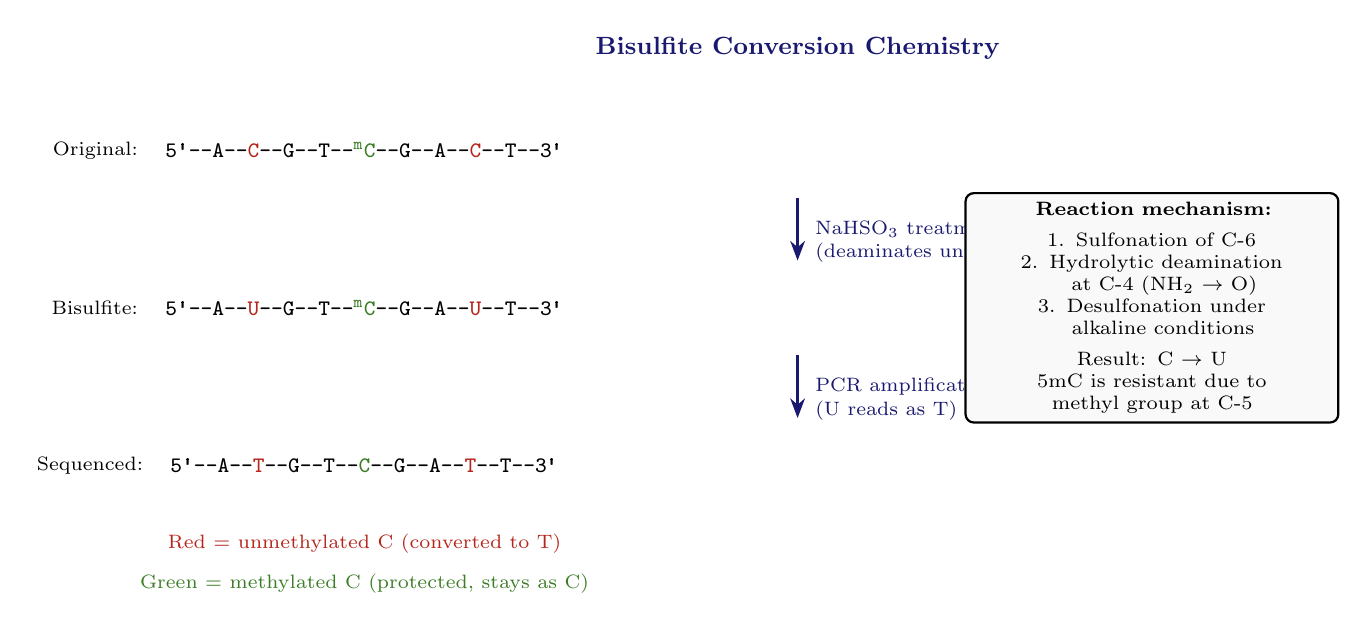
\begin{tikzpicture}[
  node distance=1.0cm,
  box/.style={draw, rounded corners=3pt, thick, minimum width=2.8cm, minimum height=0.9cm, align=center, font=\small},
  chem/.style={font=\footnotesize\ttfamily, align=center},
  arrow/.style={-{Stealth[length=2.5mm]}, thick},
  label/.style={font=\scriptsize, text width=3cm, align=center}
]

% Title
\node[font=\bfseries\small, MidnightBlue] at (5.5,6.5) {Bisulfite Conversion Chemistry};

% Original DNA strand
\node[chem] (orig) at (0,5.2) {5\textquotesingle--A--\textcolor{BrickRed}{\textbf{C}}--G--T--\textcolor{OliveGreen}{\textbf{\textsuperscript{m}C}}--G--A--\textcolor{BrickRed}{\textbf{C}}--T--3\textquotesingle};
\node[font=\scriptsize, left=0.1cm of orig] {Original:};

% Bisulfite treatment arrow
\draw[arrow, MidnightBlue] (5.5,4.6) -- (5.5,3.8);
\node[font=\scriptsize, MidnightBlue, right] at (5.6,4.2) {NaHSO\textsubscript{3} treatment};
\node[font=\scriptsize, MidnightBlue, right] at (5.6,3.9) {(deaminates unmodified C $\rightarrow$ U)};

% After bisulfite
\node[chem] (bisulf) at (0,3.2) {5\textquotesingle--A--\textcolor{BrickRed}{\textbf{U}}--G--T--\textcolor{OliveGreen}{\textbf{\textsuperscript{m}C}}--G--A--\textcolor{BrickRed}{\textbf{U}}--T--3\textquotesingle};
\node[font=\scriptsize, left=0.1cm of bisulf] {Bisulfite:};

% PCR arrow
\draw[arrow, MidnightBlue] (5.5,2.6) -- (5.5,1.8);
\node[font=\scriptsize, MidnightBlue, right] at (5.6,2.2) {PCR amplification};
\node[font=\scriptsize, MidnightBlue, right] at (5.6,1.9) {(U reads as T)};

% After PCR
\node[chem] (pcr) at (0,1.2) {5\textquotesingle--A--\textcolor{BrickRed}{\textbf{T}}--G--T--\textcolor{OliveGreen}{\textbf{C}}--G--A--\textcolor{BrickRed}{\textbf{T}}--T--3\textquotesingle};
\node[font=\scriptsize, left=0.1cm of pcr] {Sequenced:};

% Legend
\node[font=\scriptsize, BrickRed] at (0, 0.2) {Red = unmethylated C (converted to T)};
\node[font=\scriptsize, OliveGreen] at (0, -0.3) {Green = methylated C (protected, stays as C)};

% Chemical detail box on right
\node[box, fill=gray!5, text width=4.5cm, font=\scriptsize] at (10, 3.2) {
  \textbf{Reaction mechanism:}\\[3pt]
  1. Sulfonation of C-6\\
  2. Hydrolytic deamination\\
  \quad at C-4 (NH\textsubscript{2} $\rightarrow$ O)\\
  3. Desulfonation under\\
  \quad alkaline conditions\\[3pt]
  Result: C $\rightarrow$ U\\
  5mC is resistant due to\\
  methyl group at C-5
};

\end{tikzpicture}
\caption[Bisulfite conversion chemistry for methylation detection.]{Bisulfite conversion chemistry. Sodium bisulfite deaminates unmethylated cytosines to uracil (read as T after PCR), while methylated cytosines (5mC, shown with superscript m) are protected and remain as C. By comparing the sequenced reads to the reference genome, each CpG site can be scored as methylated or unmethylated.}
\label{fig:methylation:bisulfite-chemistry}
\end{figure}

\begin{warningbox}
Standard bisulfite sequencing \textbf{cannot distinguish 5mC from 5hmC}. Both modifications are resistant to bisulfite deamination and appear as ``C'' in the sequencing output. To differentiate these marks, specialised methods such as oxidative bisulfite sequencing (oxBS-seq) or TET-assisted bisulfite sequencing (TAB-seq) are required (see \cref{subsec:methylation:oxbs-tab}).
\end{warningbox}

\subsection{Bisulfite Conversion Chemistry in Detail}
\label{subsec:methylation:bisulfite-chemistry}

The bisulfite conversion of cytosine proceeds through a well-characterised three-step chemical mechanism. Understanding this mechanism is essential for appreciating why the reaction discriminates between methylated and unmethylated cytosines, and for diagnosing conversion failures.

\subsubsection{The Deamination Mechanism}

The conversion of unmethylated cytosine to uracil by sodium bisulfite involves three sequential reactions:

\begin{enumerate}[itemsep=3pt]
  \item \textbf{Sulfonation (addition):} Bisulfite ion ($\text{HSO}_3^{-}$) attacks the C-6 position of the cytosine ring in a reversible nucleophilic addition, forming \textbf{cytosine-6-sulfonate}. This reaction requires acidic conditions (pH 5.0--5.5) and proceeds efficiently only on single-stranded DNA, because bisulfite cannot access cytosines in double-stranded regions.
  \item \textbf{Hydrolytic deamination:} The amino group ($-\text{NH}_2$) at the C-4 position of cytosine-6-sulfonate undergoes hydrolytic deamination, replacing $-\text{NH}_2$ with a carbonyl group ($=\text{O}$), yielding \textbf{uracil-6-sulfonate}. This is the rate-limiting step and is accelerated by elevated temperature (typically 50--70\textdegree{}C) and prolonged incubation (2--16 hours).
  \item \textbf{Alkali desulfonation:} Under alkaline conditions (pH $>$ 12, achieved during the final desulfonation/clean-up step), the sulfonate group is eliminated from C-6, yielding \textbf{uracil}.
\end{enumerate}

The overall reaction can be summarised as:
\begin{equation}
\label{eq:methylation:bisulfite-overall}
\text{Cytosine} \xrightarrow{\text{HSO}_3^{-},\;\text{pH}\,5} \text{Cytosine-6-sulfonate} \xrightarrow{\text{H}_2\text{O},\;\Delta} \text{Uracil-6-sulfonate} \xrightarrow{\text{OH}^{-}} \text{Uracil}
\end{equation}

\subsubsection{Why 5-Methylcytosine Is Resistant}

The methyl group at the C-5 position of 5mC sterically and electronically hinders the initial sulfonation reaction at C-6. Specifically:
\begin{itemize}[itemsep=2pt]
  \item The electron-donating methyl group increases the electron density at C-5 and C-6, making the ring less electrophilic and thus less susceptible to nucleophilic attack by bisulfite.
  \item The steric bulk of the methyl group physically impedes access of $\text{HSO}_3^{-}$ to C-6.
  \item As a result, the sulfonation rate for 5mC is approximately \textbf{100-fold slower} than for unmodified cytosine under standard bisulfite conditions.
\end{itemize}

5-Hydroxymethylcytosine (5hmC) is similarly resistant to bisulfite-mediated deamination. The hydroxymethyl group at C-5 provides comparable steric and electronic protection, which is why standard bisulfite sequencing cannot distinguish 5mC from 5hmC.

\subsubsection{Conversion Rate and Completeness}

The efficiency of bisulfite conversion is characterised by two complementary metrics:

\begin{align}
\label{eq:methylation:conversion-rate}
\text{Conversion rate} &= \frac{\text{Number of unmethylated C read as T}}{\text{Total unmethylated C positions}} \geq 99.0\% \\[6pt]
\label{eq:methylation:protection-rate}
\text{Protection rate} &= \frac{\text{Number of methylated C read as C}}{\text{Total methylated C positions}} \geq 99.0\%
\end{align}

A high-quality bisulfite experiment achieves:
\begin{itemize}[itemsep=2pt]
  \item \textbf{Conversion rate $> 99\%$} for unmethylated cytosines (i.e., $< 1\%$ false methylation).
  \item \textbf{Protection rate $> 99\%$} for methylated cytosines (i.e., $< 1\%$ false non-methylation).
  \item The non-conversion rate (complement of conversion rate) directly translates to \textbf{false-positive methylation calls}, which can be devastating for analyses of lowly methylated regions.
\end{itemize}

\subsubsection{Conversion Rate Quality Control}
\label{subsubsec:methylation:conversion-qc}

Conversion rate is routinely assessed using two approaches:

\textbf{Spike-in controls:}
\begin{itemize}[itemsep=2pt]
  \item \textbf{Lambda phage DNA} ($\sim$0.5--1\% of library): the lambda phage genome (\species{Enterobacteria phage $\lambda$}) is unmethylated. After bisulfite treatment, virtually all cytosines in the lambda genome should read as T. The conversion rate is calculated as:
\end{itemize}
\begin{equation}
\label{eq:methylation:lambda-conversion}
\text{Conversion rate}_{\lambda} = \frac{T_{\lambda}}{T_{\lambda} + C_{\lambda}}
\end{equation}
where $T_{\lambda}$ and $C_{\lambda}$ are the total thymine and cytosine counts at all cytosine positions in reads mapping to the lambda genome.
\begin{itemize}[itemsep=2pt]
  \item \textbf{pUC19 plasmid} (CpG-methylated): used to verify that methylated cytosines are protected. The protection rate should exceed 99\%.
\end{itemize}

\textbf{Non-CpG context methylation:}
\begin{itemize}[itemsep=2pt]
  \item In most somatic mammalian cells, cytosine methylation occurs almost exclusively in the CpG context. Methylation measured in the \textbf{CHH and CHG contexts} (where H = A, T, or C) therefore predominantly reflects \textbf{incomplete bisulfite conversion} rather than true non-CpG methylation.
  \item The non-CpG apparent methylation rate serves as an internal conversion control:
\end{itemize}
\begin{equation}
\label{eq:methylation:chh-conversion}
\text{Estimated non-conversion} \approx \frac{C_{\text{CHH}}}{C_{\text{CHH}} + T_{\text{CHH}}}
\end{equation}

\begin{warningbox}
Incomplete bisulfite conversion inflates methylation estimates across the entire genome, but its impact is most severe at lowly methylated loci. For example, if the non-conversion rate is 2\%, a truly unmethylated CpG will appear 2\% methylated, while a 50\% methylated CpG will be measured as 51\%. This makes regions with low methylation levels (enhancers, partially methylated domains in cancer) particularly susceptible to artefacts. Samples with conversion rates below 98\% should generally be discarded and re-processed.
\end{warningbox}

\begin{tipbox}
When using cell types known to have genuine non-CpG methylation---such as embryonic stem cells, neurons, or oocytes---the CHH/CHG context cannot be used as an internal conversion control. In these cases, the lambda phage spike-in becomes essential. Always include spike-in controls in experimental designs involving these cell types.
\end{tipbox}

\subsection{Whole-Genome Bisulfite Sequencing (WGBS)}
\label{subsec:methylation:wgbs}

\acrfull{WGBS} is the gold standard for genome-wide methylation profiling at single-base resolution. It interrogates the methylation status of every cytosine in the genome (approximately 28 million CpG sites in the human genome, plus non-CpG sites).

\begin{protocolbox}[title={WGBS Library Preparation}]
\textbf{Pre-bisulfite (standard) method:}
\begin{enumerate}[itemsep=1pt]
  \item Fragment genomic DNA to 200--400\basepair{} (sonication or enzymatic).
  \item End repair, A-tailing, adapter ligation (methylated adapters to survive bisulfite treatment).
  \item Size selection (gel or bead-based).
  \item Bisulfite conversion (sodium bisulfite, 2--16 hours at elevated temperature).
  \item PCR amplification with adapter primers.
  \item Library QC and sequencing.
\end{enumerate}

\textbf{Post-Bisulfite Adapter Tagging (PBAT):}
\begin{enumerate}[itemsep=1pt]
  \item Bisulfite-convert genomic DNA \textit{first}.
  \item Synthesise first strand using random primers with adapters.
  \item Synthesise second strand with another random-adapter primer.
  \item Amplify and sequence.
\end{enumerate}
PBAT avoids DNA loss from bisulfite degradation of adapter-ligated molecules and works with lower input ($< 100$\,ng). It is the basis for low-input and single-cell bisulfite methods.
\end{protocolbox}

\subsubsection{Coverage Requirements}

WGBS requires substantial sequencing depth because bisulfite conversion reduces sequence complexity (all unmethylated Cs become Ts), making alignment more challenging and reducing effective coverage:

\begin{itemize}[itemsep=2pt]
  \item \textbf{Minimum useful depth:} 5--10$\times$ per strand (10--20$\times$ total) for global methylation patterns.
  \item \textbf{Standard depth:} 30$\times$ for reliable single-CpG-resolution analysis.
  \item \textbf{DMR detection:} Requires $\geq$ 10 reads per CpG for statistical testing of differentially methylated regions.
  \item For a human genome at 30$\times$: approximately 900 million 150\basepair{} PE reads (270\,Gb of data).
\end{itemize}

\begin{tipbox}
Spike-in unmethylated lambda phage DNA ($\sim$0.5--1\% of the library) or methylated pUC19 plasmid as conversion controls. Lambda DNA should show $>$99\% conversion (all Cs read as T), while pUC19 should remain $>$99\% methylated. Conversion rates $<$ 98\% indicate incomplete bisulfite treatment and the data should be discarded.
\end{tipbox}

\subsubsection{Alignment Challenges}

Bisulfite-converted reads have reduced sequence complexity because all Cs on the original strand that were unmethylated are now Ts. This creates alignment difficulties:

\begin{itemize}[itemsep=2pt]
  \item The effective four-letter alphabet is reduced to a three-letter alphabet on the converted strand.
  \item Reads can originate from either the Watson (original top) or Crick (original bottom) strand, and bisulfite conversion is strand-specific.
  \item Specialised aligners handle this by performing \textit{in silico} C-to-T conversion of both reads and reference, aligning in the converted space, and then mapping back to the original reference.
\end{itemize}

\subsubsection{Dedicated Bisulfite Aligners}

\begin{table}[htbp]
\centering
\caption{Comparison of bisulfite-seq alignment tools.}
\label{tab:methylation:aligners}
\small
\begin{tabularx}{\textwidth}{l X l l l}
\toprule
\textbf{Aligner} & \textbf{Algorithm} & \textbf{Speed} & \textbf{Memory} & \textbf{Notes} \\
\midrule
Bismark & Bowtie2/HISAT2 backend; three-letter aligner & Moderate & Moderate & Most widely used; excellent documentation \\
\addlinespace
bwa-meth & BWA-MEM backend; in silico conversion & Fast & Low--moderate & Faster than Bismark; good for large datasets \\
\addlinespace
BSBolt & Combined aligner and methylation caller & Fast & Moderate & Integrated pipeline; PBAT support \\
\addlinespace
BSMAP & Seed-based; wildcard approach & Fast & High & Legacy tool; still used \\
\addlinespace
gemBS & Full pipeline (alignment + calling) & Fast & High & Designed for large cohorts \\
\bottomrule
\end{tabularx}
\end{table}

\subsection{Reduced Representation Bisulfite Sequencing (RRBS)}
\label{subsec:methylation:rrbs}

RRBS is a cost-effective alternative to WGBS that enriches for CpG-rich regions of the genome:

\begin{protocolbox}[title={RRBS Protocol}]
\begin{enumerate}[itemsep=1pt]
  \item Digest genomic DNA with \textbf{MspI} (recognition site: C$\wedge$CGG), which cuts at CpG-containing sequences regardless of methylation status.
  \item End repair and A-tailing (fragments have predictable CG-rich ends).
  \item Adapter ligation.
  \item Size selection: typically 150--400\basepair{} fragments, which enriches for CpG islands and CpG-dense regions.
  \item Bisulfite conversion.
  \item PCR amplification and sequencing.
\end{enumerate}
\end{protocolbox}

RRBS covers approximately 10--12\% of all CpGs in the human genome (about 3 million CpGs), but captures the majority of CpG islands and promoter-associated CpGs. It requires only 10--30 million reads per sample, making it roughly 10--30$\times$ cheaper than WGBS.

\begin{warningbox}
RRBS has important limitations: (1) it is restricted to regions flanking MspI cut sites and therefore misses many enhancers, intergenic regions, and CpG-poor regulatory elements; (2) the fragment ends contain CpG sites that were part of the MspI recognition sequence---these should be excluded from methylation calling due to end-repair artefacts (tools like Trim Galore's \texttt{--rrbs} flag handle this); (3) coverage is highly non-uniform, with some CpGs having thousands of reads and others having none.
\end{warningbox}

%% ============================================================
\section{Enzymatic Methyl-seq (EM-seq)}
\label{sec:methylation:emseq}

Enzymatic methyl-seq (EM-seq), commercialised as the NEBNext Enzymatic Methyl-seq (EM-seq) kit by New England Biolabs, is a gentler alternative to bisulfite conversion that avoids the harsh chemical treatment responsible for DNA degradation.

\subsection{Principle}
\label{subsec:methylation:emseq-principle}

EM-seq uses a two-step enzymatic process:

\begin{enumerate}[itemsep=3pt]
  \item \textbf{TET2 oxidation:} The TET2 enzyme (plus an oxidation supplement) converts 5mC to 5-carboxylcytosine (5caC) and 5hmC to 5caC. These oxidised forms are resistant to the subsequent deamination step.
  \item \textbf{APOBEC3A deamination:} The APOBEC3A enzyme deaminates \textit{unmodified} cytosines to uracils, mimicking the bisulfite conversion outcome. Importantly, APOBEC3A does not deaminate the oxidised forms (5caC), so originally methylated and hydroxymethylated cytosines are protected.
\end{enumerate}

The net result is the same readout as bisulfite sequencing (unmethylated C $\rightarrow$ T, methylated C $\rightarrow$ C), but with critical advantages:

\begin{itemize}[itemsep=2pt]
  \item \textbf{Less DNA damage:} bisulfite treatment degrades 90--99\% of input DNA; EM-seq preserves DNA integrity.
  \item \textbf{Lower input requirements:} works reliably with 10--100\,ng of DNA (vs.\ 200\,ng--1\,$\mu$g for standard WGBS).
  \item \textbf{Better coverage uniformity:} reduced GC bias and more even coverage across the genome.
  \item \textbf{More accurate at low-methylated regions:} less false methylation signal from incomplete conversion.
\end{itemize}

\begin{tipbox}
EM-seq is rapidly becoming the preferred method for genome-wide methylation profiling, especially when input DNA is limited (FFPE samples, liquid biopsies, sorted cell populations). If you are starting a new methylation project and do not have a specific reason to use bisulfite, consider EM-seq as the default choice.
\end{tipbox}

%% ============================================================
\section{Distinguishing 5mC from 5hmC}
\label{sec:methylation:5hmc}

\subsection{Oxidative Bisulfite Sequencing (oxBS-seq)}
\label{subsec:methylation:oxbs-tab}

Standard bisulfite sequencing reads both 5mC and 5hmC as ``C.'' To distinguish them:

\textbf{oxBS-seq} adds a chemical oxidation step (potassium perruthenate, KRuO\textsubscript{4}) \textit{before} bisulfite treatment. This oxidises 5hmC to 5-formylcytosine (5fC), which is then deaminated by bisulfite (read as T). Thus:

\begin{itemize}[itemsep=2pt]
  \item In standard BS-seq: 5mC $\rightarrow$ C, 5hmC $\rightarrow$ C, C $\rightarrow$ T.
  \item In oxBS-seq: 5mC $\rightarrow$ C, 5hmC $\rightarrow$ T, C $\rightarrow$ T.
  \item 5hmC levels at each site = BS-seq methylation $-$ oxBS-seq methylation.
\end{itemize}

\subsection{TET-Assisted Bisulfite Sequencing (TAB-seq)}

TAB-seq specifically maps 5hmC:

\begin{enumerate}[itemsep=2pt]
  \item Protect 5hmC by glucosylation using $\beta$-glucosyltransferase ($\beta$-GT) to form 5-glucosylhydroxymethylcytosine (5ghmC).
  \item Oxidise 5mC to 5caC using recombinant TET1 enzyme.
  \item Bisulfite conversion: unmodified C and 5caC are deaminated (read as T), while 5ghmC is protected (read as C).
  \item Result: only 5hmC positions read as C; everything else reads as T.
\end{enumerate}

\subsection{ACE-seq}

APOBEC-Coupled Epigenetic Sequencing (ACE-seq) uses APOBEC3A enzyme instead of bisulfite for 5hmC detection. APOBEC3A deaminates C, 5mC, and 5fC but \textit{not} 5hmC (or its glucosylated form). Combined with $\beta$-GT protection, this provides a bisulfite-free 5hmC mapping method with less DNA damage.

%% ============================================================
\section{Targeted Methylation Approaches}
\label{sec:methylation:targeted}

\subsection{Methyl-Capture Sequencing}

Target-enrichment (hybridisation capture) can be combined with bisulfite sequencing to interrogate a defined subset of the genome:

\begin{itemize}[itemsep=2pt]
  \item \textbf{Agilent SureSelect Methyl-Seq:} captures 3.7 million CpGs (84 Mb target region) covering CpG islands, shores, shelves, and ENCODE regulatory elements.
  \item \textbf{Roche SeqCap Epi CpGiant:} captures 5.5 million CpGs.
  \item These methods provide deep coverage of biologically relevant CpGs at a fraction of WGBS cost.
\end{itemize}

\subsection{Methylation Arrays}

Illumina methylation arrays use bisulfite-converted DNA hybridised to bead arrays with methylation-specific probes:

\begin{itemize}[itemsep=2pt]
  \item \textbf{Infinium MethylationEPIC v2.0:} interrogates $\sim$935,000 CpG sites. The most widely used array platform, especially for large epidemiological cohorts.
  \item Provides a beta value (0--1) for each CpG representing the fraction of methylated alleles.
  \item Advantages: low cost per sample, high throughput, extensive normalization pipelines.
  \item Limitations: fixed probe set (biased towards CpG islands), limited to pre-selected sites.
\end{itemize}

%% ============================================================
\section{Long-Read Methylation Detection}
\label{sec:methylation:longread}

\subsection{Nanopore Direct Methylation Detection}
\label{subsec:methylation:nanopore}

Oxford Nanopore sequencing can detect DNA modifications \textbf{directly from the raw ionic current signal} without any chemical conversion. As a DNA strand passes through the nanopore, modified bases produce subtly different current signatures compared to unmodified bases:

\begin{itemize}[itemsep=3pt]
  \item \textbf{Simultaneous detection} of 5mC, 5hmC, and 6mA from a single sequencing run.
  \item \textbf{No chemical conversion} means no DNA damage, no conversion bias, and no loss of long-range information.
  \item \textbf{Single-molecule resolution:} methylation is called on individual reads, enabling analysis of allele-specific methylation and methylation heterogeneity.
  \item \textbf{Long reads} provide methylation information in the context of phased haplotypes.
\end{itemize}

Key tools for nanopore methylation calling:

\begin{itemize}[itemsep=2pt]
  \item \textbf{Dorado:} ONT's current basecaller with integrated modification calling (replaces Guppy). Outputs modified base probabilities in BAM tags (MM/ML).
  \item \textbf{modkit:} ONT's tool for summarising, filtering, and extracting modification calls from BAM files.
  \item \textbf{Remora:} Deep learning framework for training custom modification-detection models.
  \item \textbf{Megalodon (legacy):} Earlier ONT tool for per-read modification calling; superseded by Dorado.
  \item \textbf{DeepMod / DeepSignal:} Third-party deep-learning tools for nanopore modification detection.
\end{itemize}

\begin{tipbox}
Nanopore methylation detection accuracy has improved dramatically. With R10.4.1 chemistry and Dorado's super-accuracy models, per-CpG-site accuracy exceeds 95\% at 10$\times$ coverage, approaching bisulfite sequencing accuracy. The key advantage is the ability to phase methylation across long reads without any chemical treatment.
\end{tipbox}

\subsection{PacBio Methylation Detection}
\label{subsec:methylation:pacbio}

PacBio SMRT sequencing detects DNA modifications through \textbf{kinetic signatures}---changes in the inter-pulse duration (IPD) when the polymerase encounters a modified base:

\begin{itemize}[itemsep=2pt]
  \item Most sensitive for \textbf{6mA} detection (strong kinetic signature).
  \item \textbf{5mC detection} from native DNA is possible but requires very high coverage ($> 50\times$) due to the weaker kinetic signature.
  \item \textbf{Improved with HiFi + 5mC model:} PacBio's \software{jasmine} tool and newer \software{primrose} model enable CpG methylation calling from HiFi reads, though sensitivity is lower than nanopore or bisulfite methods.
  \item Best used as an additional data layer when HiFi sequencing is already being performed for other purposes (e.g., genome assembly, variant calling).
\end{itemize}

%% ============================================================
\section{Comprehensive Comparison of Methylation Methods}
\label{sec:methylation:comparison}

\begin{table}[htbp]
\centering
\caption[Comparison of DNA methylation profiling methods.]{Comparison of major DNA methylation profiling approaches.}
\label{tab:methylation:comparison}
\small
\begin{tabularx}{\textwidth}{l c c c c X}
\toprule
\textbf{Method} & \textbf{Resolution} & \textbf{Coverage} & \textbf{Input} & \textbf{Cost} & \textbf{Key Features} \\
\midrule
WGBS & Single base & Genome-wide & 200\,ng--1\,$\mu$g & \$\$\$\$ & Gold standard; complete CpG coverage \\
\addlinespace
RRBS & Single base & CpG-rich ($\sim$10\%) & 10--100\,ng & \$\$ & Cost-effective; biased to CpG islands \\
\addlinespace
EM-seq & Single base & Genome-wide & 10--100\,ng & \$\$\$\$ & Less DNA damage; low input \\
\addlinespace
oxBS-seq & Single base & Genome-wide & 1--2\,$\mu$g & \$\$\$\$\$ & Distinguishes 5mC from 5hmC \\
\addlinespace
TAB-seq & Single base & Genome-wide & 1\,$\mu$g & \$\$\$\$\$ & Maps 5hmC specifically \\
\addlinespace
Methyl-capture & Single base & Targeted ($\sim$3--5M CpGs) & 250\,ng & \$\$\$ & Good compromise of cost and coverage \\
\addlinespace
EPIC array & Single probe & $\sim$935K CpGs & 250\,ng & \$ & Cheapest per sample; large cohorts \\
\addlinespace
Nanopore & Single base & Genome-wide & 1\,$\mu$g & \$\$\$ & No conversion; 5mC+5hmC+6mA; long reads \\
\addlinespace
PacBio HiFi & Single base & Genome-wide & 5--10\,$\mu$g & \$\$\$\$ & CpG methylation from kinetics; long reads \\
\bottomrule
\end{tabularx}
\end{table}

%% ============================================================
\section{Bioinformatics Workflow for Bisulfite Sequencing}
\label{sec:methylation:bioinformatics}

The standard WGBS/EM-seq analysis pipeline follows these steps:

\begin{enumerate}[itemsep=2pt]
  \item \textbf{Quality control:} FastQC, MultiQC to assess raw read quality.
  \item \textbf{Adapter trimming:} Trim Galore (wrapper around Cutadapt) with bisulfite-specific options.
  \item \textbf{Alignment:} Bismark or bwa-meth against a bisulfite-converted reference genome.
  \item \textbf{Deduplication:} Remove PCR duplicates (Bismark \texttt{deduplicate\_bismark} or Picard).
  \item \textbf{Methylation extraction:} Extract per-CpG methylation levels (Bismark \texttt{bismark\_methylation\_extractor} or \software{MethylDackel}).
  \item \textbf{Quality assessment:} Check conversion rate (lambda control), M-bias plots, coverage distribution.
  \item \textbf{Differential methylation analysis:} Identify DMRs using DSS, dmrseq, methylKit, or BSmooth.
  \item \textbf{Visualisation:} IGV tracks, heatmaps, genome browser.
\end{enumerate}

\subsection{Snakemake Workflow}
\label{subsec:methylation:snakemake}

\begin{lstlisting}[language=Python, caption={Snakemake workflow for WGBS analysis with Bismark.}, label={lst:methylation:snakemake}]
# Snakefile for WGBS analysis using Bismark
configfile: "config.yaml"

SAMPLES = config["samples"]
GENOME_DIR = config["genome_dir"]

rule all:
    input:
        "results/multiqc/multiqc_report.html",
        expand("results/methylation/{sample}.bismark.cov.gz",
               sample=SAMPLES),
        expand("results/methylation/{sample}_CpG_report.txt",
               sample=SAMPLES),
        "results/dmr/dmrseq_results.tsv"

rule trim_galore:
    input:
        r1 = "raw_data/{sample}_R1.fastq.gz",
        r2 = "raw_data/{sample}_R2.fastq.gz"
    output:
        r1 = "results/trimmed/{sample}_R1_val_1.fq.gz",
        r2 = "results/trimmed/{sample}_R2_val_2.fq.gz",
        report1 = "results/trimmed/{sample}_R1.fastq.gz_trimming_report.txt",
        report2 = "results/trimmed/{sample}_R2.fastq.gz_trimming_report.txt"
    threads: 4
    conda: "envs/trim_galore.yaml"
    shell:
        """
        trim_galore --paired --cores {threads} \
            --output_dir results/trimmed \
            {input.r1} {input.r2}
        """

rule bismark_genome_preparation:
    input:
        genome = GENOME_DIR
    output:
        directory(GENOME_DIR + "/Bisulfite_Genome")
    conda: "envs/bismark.yaml"
    shell:
        """
        bismark_genome_preparation {input.genome}
        """

rule bismark_align:
    input:
        r1 = "results/trimmed/{sample}_R1_val_1.fq.gz",
        r2 = "results/trimmed/{sample}_R2_val_2.fq.gz",
        genome = GENOME_DIR,
        idx = GENOME_DIR + "/Bisulfite_Genome"
    output:
        bam = "results/aligned/{sample}_pe.bam",
        report = "results/aligned/{sample}_PE_report.txt"
    threads: 8
    resources:
        mem_mb = 32000
    conda: "envs/bismark.yaml"
    shell:
        """
        bismark --genome {input.genome} \
            -1 {input.r1} -2 {input.r2} \
            --parallel {threads} \
            --output_dir results/aligned \
            --temp_dir results/tmp \
            --non_directional  # Add if using PBAT library
        """

rule bismark_dedup:
    input:
        bam = "results/aligned/{sample}_pe.bam"
    output:
        bam = "results/dedup/{sample}_pe.deduplicated.bam",
        report = "results/dedup/{sample}_pe.deduplication_report.txt"
    conda: "envs/bismark.yaml"
    shell:
        """
        deduplicate_bismark --paired --bam \
            --output_dir results/dedup \
            {input.bam}
        """

rule methylation_extraction:
    input:
        bam = "results/dedup/{sample}_pe.deduplicated.bam",
        genome = GENOME_DIR
    output:
        cov = "results/methylation/{sample}.bismark.cov.gz",
        cpg = "results/methylation/{sample}_CpG_report.txt",
        mbias = "results/methylation/{sample}_pe.deduplicated.M-bias.txt"
    threads: 4
    conda: "envs/bismark.yaml"
    shell:
        """
        bismark_methylation_extractor --paired-end \
            --comprehensive --merge_non_CpG \
            --multicore {threads} \
            --cytosine_report --genome_folder {input.genome} \
            --bedGraph --gzip \
            --output results/methylation \
            {input.bam}
        """

rule dmr_analysis:
    input:
        cpg_reports = expand(
            "results/methylation/{sample}_CpG_report.txt",
            sample=SAMPLES
        )
    output:
        dmrs = "results/dmr/dmrseq_results.tsv",
        plots = "results/dmr/dmr_plots.pdf"
    conda: "envs/dmrseq.yaml"
    script:
        "scripts/run_dmrseq.R"

rule multiqc:
    input:
        expand("results/trimmed/{sample}_R1.fastq.gz_trimming_report.txt",
               sample=SAMPLES),
        expand("results/aligned/{sample}_PE_report.txt",
               sample=SAMPLES),
        expand("results/dedup/{sample}_pe.deduplication_report.txt",
               sample=SAMPLES),
        expand("results/methylation/{sample}_pe.deduplicated.M-bias.txt",
               sample=SAMPLES)
    output:
        "results/multiqc/multiqc_report.html"
    conda: "envs/multiqc.yaml"
    shell:
        """
        multiqc results/ -o results/multiqc --force
        """
\end{lstlisting}

\subsection{Nextflow Workflow}
\label{subsec:methylation:nextflow}

\begin{lstlisting}[language=Java, caption={Nextflow DSL2 workflow for WGBS analysis.}, label={lst:methylation:nextflow}]
#!/usr/bin/env nextflow
nextflow.enable.dsl=2

// Parameters
params.reads     = "raw_data/*_R{1,2}.fastq.gz"
params.genome    = "reference/genome.fa"
params.outdir    = "results"

// Processes
process TRIM_GALORE {
    tag "$sample_id"
    cpus 4
    publishDir "${params.outdir}/trimmed", mode: 'copy'
    conda 'bioconda::trim-galore=0.6.10'

    input:
    tuple val(sample_id), path(reads)

    output:
    tuple val(sample_id), path("*_val_{1,2}.fq.gz"), emit: trimmed
    path "*_trimming_report.txt",                     emit: reports

    script:
    """
    trim_galore --paired --cores ${task.cpus} \
        ${reads[0]} ${reads[1]}
    """
}

process BISMARK_INDEX {
    cpus 8
    memory '32 GB'
    conda 'bioconda::bismark=0.24.2'

    input:
    path genome

    output:
    path "BissulfiteGenome", emit: index

    script:
    """
    mkdir -p genome_dir
    cp ${genome} genome_dir/
    bismark_genome_preparation genome_dir/
    mv genome_dir/Bisulfite_Genome BisulfiteGenome
    """
}

process BISMARK_ALIGN {
    tag "$sample_id"
    cpus 8
    memory '32 GB'
    publishDir "${params.outdir}/aligned", mode: 'copy'
    conda 'bioconda::bismark=0.24.2'

    input:
    tuple val(sample_id), path(reads)
    path index

    output:
    tuple val(sample_id), path("*.bam"),  emit: bam
    path "*_report.txt",                  emit: report

    script:
    """
    bismark --genome . \
        -1 ${reads[0]} -2 ${reads[1]} \
        --parallel ${task.cpus} \
        --temp_dir tmp/
    """
}

process DEDUPLICATE {
    tag "$sample_id"
    publishDir "${params.outdir}/dedup", mode: 'copy'
    conda 'bioconda::bismark=0.24.2'

    input:
    tuple val(sample_id), path(bam)

    output:
    tuple val(sample_id), path("*.deduplicated.bam"), emit: bam
    path "*.deduplication_report.txt",                emit: report

    script:
    """
    deduplicate_bismark --paired --bam ${bam}
    """
}

process METHYLATION_EXTRACTION {
    tag "$sample_id"
    cpus 4
    publishDir "${params.outdir}/methylation", mode: 'copy'
    conda 'bioconda::bismark=0.24.2'

    input:
    tuple val(sample_id), path(bam)
    path genome

    output:
    tuple val(sample_id), path("*.cov.gz"),       emit: coverage
    tuple val(sample_id), path("*CpG_report.txt"),emit: cpg_report
    path "*.M-bias.txt",                          emit: mbias

    script:
    """
    bismark_methylation_extractor --paired-end \
        --comprehensive --merge_non_CpG \
        --multicore ${task.cpus} \
        --cytosine_report --genome_folder . \
        --bedGraph --gzip \
        ${bam}
    """
}

process DMR_ANALYSIS {
    publishDir "${params.outdir}/dmr", mode: 'copy'
    conda 'bioconda::bioconductor-dmrseq=1.18.0'

    input:
    path cpg_reports

    output:
    path "dmrseq_results.tsv", emit: dmrs
    path "dmr_plots.pdf",      emit: plots

    script:
    """
    Rscript ${projectDir}/scripts/run_dmrseq.R \
        --input_dir . \
        --output_dir .
    """
}

process MULTIQC {
    publishDir "${params.outdir}/multiqc", mode: 'copy'
    conda 'bioconda::multiqc=1.21'

    input:
    path '*'

    output:
    path "multiqc_report.html"

    script:
    """
    multiqc . --force
    """
}

// Workflow
workflow {
    // Create channel from read pairs
    reads_ch = Channel
        .fromFilePairs(params.reads, checkIfExists: true)

    // Run pipeline
    TRIM_GALORE(reads_ch)
    BISMARK_INDEX(file(params.genome))
    BISMARK_ALIGN(TRIM_GALORE.out.trimmed, BISMARK_INDEX.out.index)
    DEDUPLICATE(BISMARK_ALIGN.out.bam)
    METHYLATION_EXTRACTION(DEDUPLICATE.out.bam, file(params.genome))
    DMR_ANALYSIS(METHYLATION_EXTRACTION.out.cpg_report.map{ it[1] }.collect())
    MULTIQC(
        TRIM_GALORE.out.reports
            .mix(BISMARK_ALIGN.out.report)
            .mix(DEDUPLICATE.out.report)
            .mix(METHYLATION_EXTRACTION.out.mbias)
            .collect()
    )
}
\end{lstlisting}

\begin{tipbox}
The nf-core community maintains \software{nf-core/methylseq}, a production-ready Nextflow pipeline for bisulfite sequencing that supports both Bismark and bwa-meth backends. For most users, this is the recommended starting point rather than building a pipeline from scratch. It includes comprehensive QC, supports EM-seq libraries, and integrates with institutional compute clusters.
\end{tipbox}

\subsection{Differential Methylation Analysis}
\label{subsec:methylation:dmr}

Identifying differentially methylated regions (DMRs) between conditions (e.g., tumour vs.\ normal, treated vs.\ control) is a central goal of methylation studies. Major tools include:

\begin{itemize}[itemsep=3pt]
  \item \textbf{DSS (Dispersion Shrinkage for Sequencing):} Bayesian hierarchical model based on the beta-binomial distribution. Handles biological variability through dispersion shrinkage. Works well with as few as two replicates per group. Provides both differentially methylated loci (DMLs) and DMRs.
  \item \textbf{dmrseq:} Specifically designed for detecting DMRs (not individual CpGs). Uses a two-stage approach: (1) identifies candidate DMR regions based on methylation differences, then (2) tests significance using a permutation-based statistic. Excellent for detecting regions with consistent, moderate methylation differences.
  \item \textbf{methylKit:} R/Bioconductor package with a complete workflow: reads coverage files, performs tiling-window or per-CpG analysis, and calls DMRs. Uses logistic regression or Fisher's exact test. Good for exploratory analysis.
  \item \textbf{BSmooth:} Smoothing-based approach that borrows information across nearby CpGs to improve estimation of local methylation levels. Particularly useful when coverage is moderate (5--15$\times$).
\end{itemize}

\subsubsection{Beta-Binomial DMR Model (DSS)}
\label{subsubsec:methylation:dss-model}

The \software{DSS} (Dispersion Shrinkage for Sequencing) package implements a rigorous statistical framework for identifying differentially methylated loci (DMLs) and regions (DMRs) from bisulfite sequencing data. The model accounts for both sampling variation (from finite read coverage) and biological variation (from inter-replicate differences) through a hierarchical Beta-Binomial framework.

\textbf{Per-CpG read-level model.} At a given CpG site $j$ in sample $i$, let $X_{ij}$ be the number of reads showing methylation (C retained) out of $n_{ij}$ total reads covering that site. Given the true methylation proportion $\theta_{ij}$, the read counts follow a Binomial distribution:
\begin{equation}
\label{eq:methylation:dss-binomial}
X_{ij} \mid \theta_{ij} \sim \text{Binomial}(n_{ij},\; \theta_{ij})
\end{equation}

\textbf{Biological variability model.} Across biological replicates within the same condition, the true methylation proportion $\theta_{ij}$ is not fixed but varies. DSS models this variability with a Beta prior:
\begin{equation}
\label{eq:methylation:dss-beta}
\theta_{ij} \sim \text{Beta}(\alpha_j,\; \beta_j)
\end{equation}
where the Beta distribution is parameterised by the mean methylation level $\mu_j = \alpha_j / (\alpha_j + \beta_j)$ and the dispersion $\phi_j = 1/(\alpha_j + \beta_j + 1)$. The dispersion parameter $\phi_j$ captures biological variability: larger $\phi_j$ implies greater heterogeneity across replicates.

\textbf{Marginal distribution.} Integrating over $\theta_{ij}$, the marginal distribution of $X_{ij}$ is Beta-Binomial:
\begin{equation}
\label{eq:methylation:dss-betabinom}
X_{ij} \sim \text{Beta-Binomial}(n_{ij},\; \alpha_j,\; \beta_j)
\end{equation}

This has variance $\text{Var}(X_{ij}) = n_{ij}\,\mu_j\,(1-\mu_j)\,[1 + (n_{ij}-1)\,\phi_j]$, which is larger than the Binomial variance by the factor $[1 + (n_{ij}-1)\,\phi_j]$, properly accounting for biological over-dispersion.

\textbf{Differential methylation testing.} To test whether methylation differs between two groups (e.g., treatment vs.\ control) at each CpG site, DSS estimates $\mu_j$ and $\phi_j$ for each group using moment estimators with \textbf{dispersion shrinkage}---borrowing information across all CpG sites to stabilise the dispersion estimates, especially when the number of replicates is small. It then applies a \textbf{Wald test} for the difference in mean methylation:
\begin{equation}
\label{eq:methylation:dss-wald}
W_j = \frac{\hat{\mu}_{j,1} - \hat{\mu}_{j,2}}{\sqrt{\widehat{\text{Var}}(\hat{\mu}_{j,1}) + \widehat{\text{Var}}(\hat{\mu}_{j,2})}}
\end{equation}
Under the null hypothesis of no differential methylation, $W_j$ approximately follows a standard normal distribution, yielding p-values that are corrected for multiple testing.

\textbf{DMR construction.} DMLs are individual CpG sites with significant p-values. DSS then merges nearby DMLs into contiguous DMRs by requiring that significant CpGs within a DMR are separated by no more than a specified distance (default: 50\basepair{}) and that the region contains a minimum number of CpGs.

\subsubsection{BSmooth Local-Likelihood Smoothing}
\label{subsubsec:methylation:bsmooth}

The \software{BSmooth} algorithm addresses a fundamental challenge in WGBS analysis: at typical sequencing depths (10--30$\times$), individual CpG sites are covered by relatively few reads, leading to noisy per-site methylation estimates. BSmooth improves these estimates by \textbf{borrowing information from neighbouring CpGs} through local-likelihood smoothing.

\textbf{Motivation.} Consider a CpG site covered by only 5 reads, of which 3 show methylation. The raw estimate of $\hat{\theta} = 0.60$ has a wide confidence interval and is unreliable. However, if the 10 neighbouring CpGs within a 1\kilobase{} window all show similar methylation levels (0.55--0.70), we can borrow strength from these neighbours to obtain a more precise estimate.

\textbf{Smoothing procedure.} BSmooth fits a \textbf{local-likelihood weighted regression} across CpG positions within a sliding window:
\begin{enumerate}[itemsep=2pt]
  \item For each CpG site, define a smoothing window containing a minimum number of CpGs (default: 70 CpGs or 1\kilobase{}, whichever spans more sites).
  \item Within this window, fit a weighted logistic regression where CpGs closer to the target site receive higher weights (using a tricube kernel function).
  \item The fitted value at the target CpG provides the smoothed methylation estimate $\tilde{\theta}_j$.
  \item Weights also incorporate coverage: CpGs with higher read depth contribute more to the fit.
\end{enumerate}

\textbf{Why smoothing works.} Methylation levels at adjacent CpGs are highly correlated---nearby CpGs tend to share similar methylation states, especially within CpG islands and shores. Smoothing exploits this spatial autocorrelation to reduce noise without sacrificing genuine biological variation that occurs over larger genomic distances.

\textbf{DMR detection with BSmooth.} After smoothing, BSmooth computes a t-statistic at each CpG comparing the smoothed methylation profiles between two groups. Contiguous regions where the t-statistic exceeds a threshold are identified as candidate DMRs, and their significance is assessed using area-under-the-curve statistics.

\begin{tipbox}
BSmooth is especially valuable for moderate-coverage WGBS experiments (5--15$\times$), where per-CpG estimates are noisy but there are sufficient neighbouring CpGs to support smoothing. At very high coverage ($>$30$\times$), the benefit of smoothing diminishes because individual CpG estimates are already precise. Conversely, in targeted sequencing (RRBS), smoothing may be unreliable because CpG coverage is fragmented and non-contiguous.
\end{tipbox}

\begin{warningbox}
A common pitfall in DMR analysis is confusing \textbf{statistical significance} with \textbf{biological significance}. With sufficient sequencing depth, even very small methylation differences (e.g., 5\%) can be statistically significant. Most biologically meaningful DMRs show methylation differences $\geq$ 20--25\%. Always apply both a statistical threshold (e.g., FDR $<$ 0.05) and a minimum methylation difference threshold (e.g., $|\Delta\beta| \geq 0.2$).
\end{warningbox}

\subsection{Visualisation}
\label{subsec:methylation:visualisation}

Methylation data can be visualised in multiple ways:

\begin{itemize}[itemsep=2pt]
  \item \textbf{Genome browser tracks:} Load Bismark coverage files (.bedGraph or .cov.gz) into IGV or the UCSC Genome Browser. Each CpG is displayed as a bar indicating methylation level (0--100\%).
  \item \textbf{Methylation heatmaps:} Cluster samples and CpG regions using tools like \software{methylKit::clusterSamples()} or deepTools \software{computeMatrix + plotHeatmap} for methylation around specific genomic features (e.g., TSSs, enhancers).
  \item \textbf{M-bias plots:} Generated by Bismark; show methylation level as a function of read position. Systematic biases at read ends (common in RRBS) indicate positions that should be excluded from methylation calling.
  \item \textbf{PCA/MDS plots:} Principal component analysis or multi-dimensional scaling of methylation data to assess sample relationships and batch effects.
  \item \textbf{Violin/bean plots:} Distribution of methylation levels across genomic features (promoters, gene bodies, repeats) by sample or condition.
\end{itemize}

%% ============================================================
\section{Experimental Design Considerations}
\label{sec:methylation:design}

\begin{keyconcept}[title={Choosing a Methylation Method}]
The choice of method depends on the experimental question:
\begin{itemize}[itemsep=2pt]
  \item \textbf{Comprehensive, unbiased survey:} WGBS or EM-seq.
  \item \textbf{CpG island--focused, budget-limited:} RRBS.
  \item \textbf{Large clinical cohorts:} EPIC array.
  \item \textbf{Distinguishing 5mC from 5hmC:} oxBS-seq, TAB-seq, or nanopore.
  \item \textbf{Low-input or degraded DNA:} EM-seq or PBAT-WGBS.
  \item \textbf{Haplotype-resolved methylation:} Nanopore or PacBio long-read sequencing.
  \item \textbf{Targeted regions of interest:} Methyl-capture or amplicon bisulfite sequencing.
\end{itemize}
\end{keyconcept}

Key design parameters to consider:

\begin{enumerate}[itemsep=3pt]
  \item \textbf{Biological replicates:} At least 3 per condition for DMR analysis; more improve statistical power.
  \item \textbf{Sequencing depth:} See coverage recommendations above; under-sequenced WGBS wastes money without providing reliable single-CpG resolution.
  \item \textbf{Batch effects:} Bisulfite conversion efficiency can vary between batches. Process all samples in a single batch or randomise samples across batches. Include conversion controls.
  \item \textbf{Cell-type composition:} Bulk tissue methylation is a weighted average of constituent cell types. Cell-type deconvolution (e.g., MethylCIBERSORT, EpiDISH) or cell sorting prior to sequencing may be necessary for accurate interpretation.
  \item \textbf{Paired samples:} When possible, pair tumour and normal samples from the same individual to reduce inter-individual variability.
\end{enumerate}

%% ============================================================
\section{Chapter Summary}
\label{sec:methylation:summary}

DNA methylation is the most extensively studied epigenetic modification, with a rich toolkit of sequencing-based methods for its detection. Bisulfite sequencing (WGBS and RRBS) remains the historical gold standard, but enzymatic methods (EM-seq) offer a gentler, more accurate alternative for new projects. Long-read technologies from Oxford Nanopore and PacBio enable direct detection of modifications without chemical conversion, providing haplotype-resolved methylation information. The choice among these methods depends on the biological question, available input material, budget, and the need to distinguish between different cytosine modifications. Rigorous bioinformatics---from specialised alignment to appropriate statistical testing of DMRs---is essential for extracting reliable biological insights from methylation data.

\chapter{Chromatin Accessibility Profiling}
\label{ch:chromatin}

\begin{keyconcept}
Chromatin accessibility refers to the degree to which nuclear DNA is physically accessible to regulatory proteins such as transcription factors, RNA polymerases, and chromatin remodelers. In eukaryotic cells, DNA is packaged around histone octamers into nucleosomes, and the local density and positioning of these nucleosomes determines whether a genomic region is ``open'' (accessible) or ``closed'' (compacted). Open chromatin regions typically correspond to active regulatory elements---promoters, enhancers, silencers, and insulators. Sequencing-based methods such as ATAC-seq and DNase-seq allow researchers to map these accessible regions genome-wide, providing a snapshot of the regulatory landscape of any cell type.
\end{keyconcept}

%% ============================================================
\section{Why Chromatin Accessibility Matters}
\label{sec:chromatin:why}

The human genome contains approximately 3.2 billion base pairs, yet only a small fraction of this sequence is accessible in any given cell type. The accessible fraction---typically 2--4\% of the genome---encompasses the active \textbf{cis-regulatory elements} that control gene expression:

\begin{itemize}[itemsep=3pt]
  \item \textbf{Active promoters:} Regions immediately upstream of transcription start sites (TSSs) where the transcription machinery assembles.
  \item \textbf{Enhancers:} Distal regulatory elements that boost transcription of target genes, often located tens to hundreds of kilobases away.
  \item \textbf{Insulators/boundary elements:} Regions that prevent inappropriate enhancer--promoter interactions, often bound by CTCF.
  \item \textbf{Silencers:} Elements that repress transcription of target genes.
  \item \textbf{Transcription factor (TF) binding sites:} Accessible DNA motifs where sequence-specific TFs bind to regulate gene expression.
\end{itemize}

Chromatin accessibility profiling provides a direct readout of regulatory element activity. Unlike histone modification mapping, which requires specific antibodies for each mark, accessibility assays capture \textit{all} open regulatory elements in a single experiment. Changes in accessibility between conditions (e.g., disease vs.\ healthy, differentiated vs.\ stem cells) reveal the regulatory programs that drive cell-state transitions.

%% ============================================================
\section{DNase-seq}
\label{sec:chromatin:dnase}

\subsection{Principle}
\label{subsec:chromatin:dnase-principle}

DNase I is an endonuclease that preferentially cleaves DNA that is not protected by nucleosomes or tightly bound proteins. Regions of open chromatin are hypersensitive to DNase I digestion, and these \textbf{DNase I hypersensitive sites (DHSs)} have been used since the 1980s to identify regulatory elements.

In \textbf{DNase-seq}:
\begin{enumerate}[itemsep=2pt]
  \item Intact nuclei are isolated from cells.
  \item Nuclei are treated with a controlled amount of DNase I enzyme.
  \item The small DNA fragments released from hypersensitive sites are size-selected (typically $<$ 300\basepair{}).
  \item Fragments are adapter-ligated and sequenced.
  \item Reads pile up at DHSs, producing peaks in the coverage signal.
\end{enumerate}

\subsection{The ENCODE Project and DHS Mapping}
\label{subsec:chromatin:encode}

DNase-seq was the method of choice for the \acrfull{ENCODE} project, which mapped DHSs in hundreds of human cell types and tissues. The ENCODE DHS maps identified approximately 2.9 million DHSs across the human genome, revealing that $\sim$40\% of the genome is accessible in at least one cell type, even though only 2--3\% is accessible in any individual cell type. This work demonstrated the vast regulatory diversity of human cells and provided a foundational resource for interpreting non-coding genetic variants.

\begin{tipbox}
While DNase-seq has been largely superseded by ATAC-seq for new experiments (due to ATAC-seq's simpler protocol and lower cell requirements), the massive DNase-seq datasets generated by ENCODE remain invaluable reference resources. The ENCODE portal (\url{https://www.encodeproject.org}) provides freely accessible DHS maps for hundreds of cell types.
\end{tipbox}

%% ============================================================
\section{ATAC-seq}
\label{sec:chromatin:atac}

\subsection{Principle: Tn5 Transposase-Mediated Tagmentation}
\label{subsec:chromatin:atac-principle}

\acrfull{ATAC-seq}, introduced by Buenrostro et al.\ in 2013, has become the dominant method for chromatin accessibility profiling. The key innovation is the use of a hyperactive \textbf{Tn5 transposase} loaded with sequencing adapters. The Tn5 transposase simultaneously fragments DNA and inserts sequencing adapters into accessible chromatin regions---a process called \textbf{tagmentation}:

\begin{enumerate}[itemsep=2pt]
  \item The Tn5 transposase can only access DNA that is not wrapped around nucleosomes or occluded by other proteins.
  \item When it inserts into accessible DNA, it creates a 9\basepair{} staggered cut and ligates sequencing adapters to both fragment ends.
  \item Nucleosome-protected regions are refractory to Tn5 insertion.
  \item After tagmentation, DNA is purified and amplified by PCR with primers complementary to the inserted adapters.
  \item Sequencing reveals the locations where Tn5 inserted, which correspond to accessible chromatin.
\end{enumerate}

\begin{figure}[htbp]
\centering
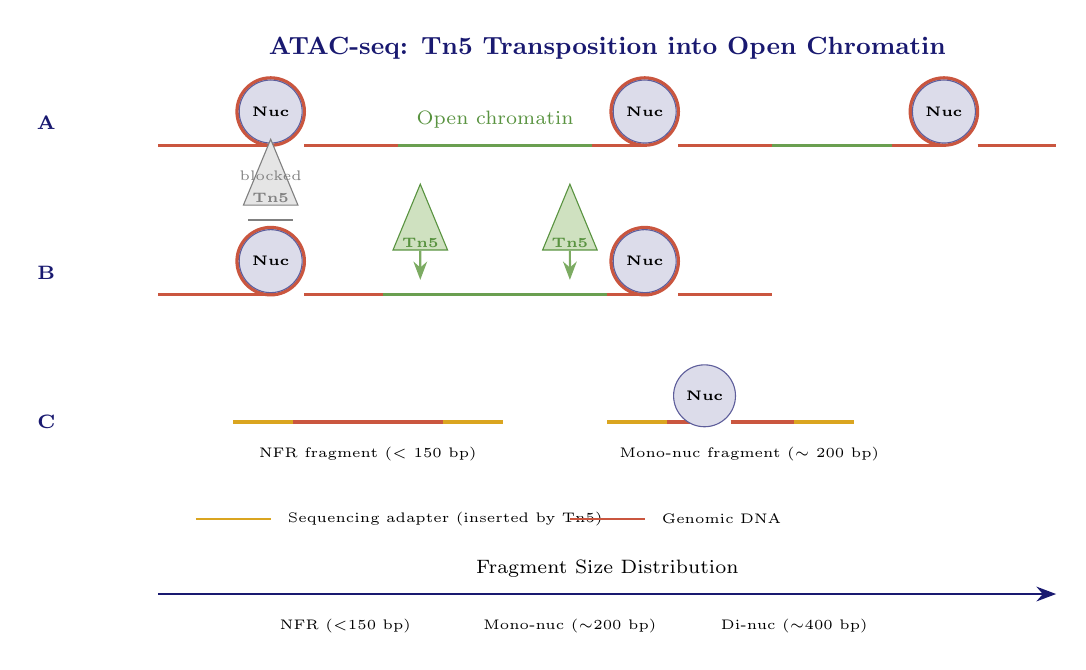
\begin{tikzpicture}[
  scale=0.95,
  nuc/.style={circle, draw=MidnightBlue!70, fill=MidnightBlue!15, minimum size=0.8cm, font=\tiny\bfseries},
  dna/.style={very thick, BrickRed!70},
  tn5/.style={isosceles triangle, draw=OliveGreen!80, fill=OliveGreen!20, minimum size=0.4cm, shape border rotate=90, inner sep=1pt, font=\tiny\bfseries},
  adapter/.style={very thick, Goldenrod},
  arrow/.style={-{Stealth[length=2.5mm]}, thick, MidnightBlue},
  label/.style={font=\scriptsize}
]

% Title
\node[font=\bfseries\small, MidnightBlue] at (6, 7.8) {ATAC-seq: Tn5 Transposition into Open Chromatin};

% --- Panel A: Chromatin with nucleosomes ---
\node[font=\scriptsize\bfseries, MidnightBlue] at (-1.5, 6.8) {A};

% Draw DNA as a line through nucleosomes
\draw[dna] (0,6.5) -- (1.5,6.5);
% Nucleosome 1
\draw[dna] (1.5,6.5) arc (-90:270:0.45);
\node[nuc] at (1.5,6.95) {Nuc};
\draw[dna] (1.95,6.5) -- (3.2,6.5);
% Open region
\draw[dna, OliveGreen!70] (3.2,6.5) -- (5.8,6.5);
\node[font=\scriptsize, OliveGreen!80, above] at (4.5,6.6) {Open chromatin};
% Nucleosome 2
\draw[dna] (5.8,6.5) -- (6.5,6.5);
\draw[dna] (6.5,6.5) arc (-90:270:0.45);
\node[nuc] at (6.5,6.95) {Nuc};
\draw[dna] (6.95,6.5) -- (8.2,6.5);
% Open region 2
\draw[dna, OliveGreen!70] (8.2,6.5) -- (9.8,6.5);
% Nucleosome 3
\draw[dna] (9.8,6.5) -- (10.5,6.5);
\draw[dna] (10.5,6.5) arc (-90:270:0.45);
\node[nuc] at (10.5,6.95) {Nuc};
\draw[dna] (10.95,6.5) -- (12,6.5);

% --- Panel B: Tn5 insertion ---
\node[font=\scriptsize\bfseries, MidnightBlue] at (-1.5, 4.8) {B};

\draw[dna] (0,4.5) -- (1.5,4.5);
\draw[dna] (1.5,4.5) arc (-90:270:0.45);
\node[nuc] at (1.5,4.95) {Nuc};
\draw[dna] (1.95,4.5) -- (3.0,4.5);

% Tn5 insertions in open region
\node[tn5] (tn5a) at (3.5,5.2) {\textcolor{OliveGreen!80}{Tn5}};
\draw[OliveGreen!60, thick, -{Stealth}] (tn5a.south) -- (3.5,4.7);
\node[tn5] (tn5b) at (5.5,5.2) {\textcolor{OliveGreen!80}{Tn5}};
\draw[OliveGreen!60, thick, -{Stealth}] (tn5b.south) -- (5.5,4.7);

\draw[dna, OliveGreen!70] (3.0,4.5) -- (6.0,4.5);

\draw[dna] (6.0,4.5) -- (6.5,4.5);
\draw[dna] (6.5,4.5) arc (-90:270:0.45);
\node[nuc] at (6.5,4.95) {Nuc};
\draw[dna] (6.95,4.5) -- (8.2,4.5);

% Blocked Tn5 at nucleosome
\node[tn5, fill=gray!20, draw=gray] (tn5c) at (1.5,5.8) {\textcolor{gray}{Tn5}};
\draw[gray, thick] (1.2,5.5) -- (1.8,5.5);
\node[font=\tiny, gray, above] at (1.5,5.9) {blocked};

% --- Panel C: Resulting fragments ---
\node[font=\scriptsize\bfseries, MidnightBlue] at (-1.5, 2.8) {C};

% NFR fragment (short)
\draw[adapter] (1,2.8) -- (1.8,2.8);
\draw[dna] (1.8,2.8) -- (3.8,2.8);
\draw[adapter] (3.8,2.8) -- (4.6,2.8);
\node[font=\tiny, below] at (2.8,2.6) {NFR fragment ($<$ 150 bp)};

% Mono-nucleosome fragment
\draw[adapter] (6,2.8) -- (6.8,2.8);
\draw[dna] (6.8,2.8) -- (7.3,2.8);
\draw[dna] (7.3,2.8) arc (-90:270:0.35);
\node[nuc, minimum size=0.55cm] at (7.3,3.15) {\tiny Nuc};
\draw[dna] (7.65,2.8) -- (8.5,2.8);
\draw[adapter] (8.5,2.8) -- (9.3,2.8);
\node[font=\tiny, below] at (7.9,2.6) {Mono-nuc fragment ($\sim$ 200 bp)};

% Legend
\draw[adapter, thick] (0.5,1.5) -- (1.5,1.5);
\node[font=\tiny, right] at (1.6,1.5) {Sequencing adapter (inserted by Tn5)};
\draw[dna, thick] (5.5,1.5) -- (6.5,1.5);
\node[font=\tiny, right] at (6.6,1.5) {Genomic DNA};

% Fragment size annotation
\draw[arrow] (0, 0.5) -- (12, 0.5);
\node[font=\scriptsize, above] at (6, 0.6) {Fragment Size Distribution};
\node[font=\tiny, below] at (2.5, 0.3) {NFR ($<$150 bp)};
\node[font=\tiny, below] at (5.5, 0.3) {Mono-nuc ($\sim$200 bp)};
\node[font=\tiny, below] at (8.5, 0.3) {Di-nuc ($\sim$400 bp)};

\end{tikzpicture}
\caption[ATAC-seq principle: Tn5 transposase tagmentation of open chromatin.]{ATAC-seq principle. (A) Chromatin consists of nucleosome-wrapped regions (closed) and nucleosome-free regions (open). (B) The Tn5 transposase, pre-loaded with sequencing adapters, preferentially inserts into accessible (open) regions. Nucleosome-bound DNA blocks Tn5 insertion. (C) The resulting fragments include short nucleosome-free region (NFR) fragments and longer mono-nucleosome fragments, producing a characteristic fragment size distribution with peaks at $<$ 150\basepair{} (NFR), $\sim$200\basepair{} (mono-nucleosomal), and $\sim$400\basepair{} (di-nucleosomal).}
\label{fig:chromatin:atac-principle}
\end{figure}

\subsection{Standard ATAC-seq Protocol}
\label{subsec:chromatin:atac-protocol}

\begin{protocolbox}[title={Standard ATAC-seq Protocol (Omni-ATAC)}]
\begin{enumerate}[itemsep=2pt]
  \item \textbf{Cell preparation:} Harvest 50,000--100,000 cells. Count cells and assess viability ($>$90\% recommended).
  \item \textbf{Lysis:} Gently lyse cells with a non-ionic detergent (e.g., 0.1\% NP-40, 0.1\% Tween-20, 0.01\% digitonin in Omni-ATAC) to release nuclei while keeping nuclei intact.
  \item \textbf{Tagmentation:} Incubate nuclei with Tn5 transposase (e.g., Illumina Tagment DNA Enzyme) at 37\textdegree{}C for 30 minutes. The enzyme simultaneously fragments and adapter-tags accessible DNA.
  \item \textbf{DNA purification:} Clean up tagmented DNA using a column or SPRI beads.
  \item \textbf{PCR amplification:} Amplify library using indexed primers (5--12 cycles, determined by qPCR to avoid over-amplification).
  \item \textbf{Size selection (optional):} Remove large fragments ($>$1000\basepair{}) by bead-based selection. Some protocols skip this.
  \item \textbf{QC:} Assess fragment size distribution on Bioanalyzer/TapeStation. A successful ATAC-seq library shows the characteristic nucleosomal laddering pattern.
  \item \textbf{Sequencing:} Paired-end 50 or 75\basepair{} reads. 50--75 million read pairs per sample recommended.
\end{enumerate}
\end{protocolbox}

\subsection{ATAC-seq Protocol Variants}
\label{subsec:chromatin:atac-variants}

Several optimised ATAC-seq protocols have been developed for specific applications:

\begin{itemize}[itemsep=3pt]
  \item \textbf{Omni-ATAC:} The recommended standard protocol. Uses a combination of detergents (NP-40 + Tween-20 + digitonin) for more complete lysis, resulting in cleaner signal and reduced mitochondrial contamination. Works across diverse cell types.
  \item \textbf{Fast-ATAC:} Optimised for blood cells and other suspension cells. Cells are tagmented directly without a separate lysis step (Tn5 + detergent in a single reaction). Reduces hands-on time and improves results for difficult cell types.
  \item \textbf{miniATAC-seq:} Designed for very low cell numbers (500--5,000 cells). Uses modifications to reduce material loss at each step.
  \item \textbf{ATAC-seq on tissues:} Fresh or flash-frozen tissues are dissociated into single nuclei (mechanical dissociation or enzymatic digestion), then standard ATAC-seq is performed. snATAC-seq on nuclei avoids the need for live cells.
  \item \textbf{mtscATAC-seq:} Modified protocol that retains mitochondrial DNA information alongside chromatin accessibility in single cells, enabling clonal tracking based on mitochondrial mutations.
\end{itemize}

\subsection{Tn5 Insertion Bias}
\label{subsec:chromatin:tn5-bias}

The Tn5 transposase has a modest sequence preference for insertion. This \textbf{Tn5 bias} can affect footprinting analysis (where exact cut-site positions are used to infer TF binding). Bias correction methods include:

\begin{itemize}[itemsep=2pt]
  \item \textbf{Naked DNA control:} Tagment purified genomic DNA (no chromatin) with Tn5 to empirically measure insertion bias.
  \item \textbf{Computational correction:} Tools like TOBIAS and seqOutBias model and correct for the Tn5 sequence preference.
  \item \textbf{k-mer-based normalisation:} Normalise cut-site frequencies by the local sequence composition.
\end{itemize}

\begin{warningbox}
A major source of wasted sequencing in ATAC-seq is \textbf{mitochondrial reads}. Because mitochondrial DNA is abundant and lacks histones (and is therefore fully accessible), mitochondrial reads can constitute 30--60\% of a standard ATAC-seq library. The Omni-ATAC protocol reduces this to $\sim$5--15\%, but filtering mitochondrial reads remains an essential bioinformatics step. Always report the fraction of mitochondrial reads as a QC metric.
\end{warningbox}

%% ============================================================
\section{Single-Cell ATAC-seq (scATAC-seq)}
\label{sec:chromatin:scatac}

\subsection{Technology and Platforms}
\label{subsec:chromatin:scatac-platforms}

Single-cell ATAC-seq (scATAC-seq) profiles chromatin accessibility in individual cells, revealing cell-type-specific regulatory landscapes within complex tissues. The dominant commercial platform is the \textbf{10x Genomics Chromium Single Cell ATAC} system:

\begin{enumerate}[itemsep=2pt]
  \item Nuclei are isolated and tagmented in bulk with Tn5.
  \item Tagmented nuclei are partitioned into nanoliter-scale gel bead-in-emulsion (GEM) droplets, each containing a single nucleus and a barcoded gel bead.
  \item Within each GEM, linear amplification attaches cell-specific barcodes to the tagmented fragments.
  \item After breaking the emulsions, all barcoded fragments are pooled, amplified, and sequenced.
  \item Demultiplexing by barcode assigns fragments to individual cells.
\end{enumerate}

Other platforms include \textbf{sci-ATAC-seq} (combinatorial indexing without droplets, enabling very high cell throughput), \textbf{SHARE-seq} (simultaneous ATAC + RNA from the same cell), and \textbf{10x Multiome} (combined scATAC + scRNA-seq from the same nucleus).

\subsection{The Sparsity Challenge}
\label{subsec:chromatin:scatac-sparsity}

scATAC-seq data is inherently \textbf{extremely sparse}. Each cell has only two copies of each autosomal locus (diploid genome), and the detection efficiency is far below 100\%. A typical scATAC-seq experiment recovers only 5,000--20,000 unique fragments per cell. The resulting cell-by-peak matrix is $>$95\% zeros, making analysis fundamentally different from scRNA-seq:

\begin{itemize}[itemsep=2pt]
  \item Individual peaks in single cells are essentially \textbf{binary} (0 or 1 fragment).
  \item Clustering and dimensionality reduction must use methods suited to binary/sparse data.
  \item Feature aggregation (peaks $\rightarrow$ gene activity scores, or peaks $\rightarrow$ TF motif scores) is essential to accumulate signal.
\end{itemize}

\subsection{Analysis Tools and Frameworks}
\label{subsec:chromatin:scatac-tools}

\begin{itemize}[itemsep=3pt]
  \item \textbf{ArchR:} Comprehensive R package for scATAC-seq analysis. Uses Arrow files for memory-efficient processing. Implements iterative LSI (latent semantic indexing) for dimensionality reduction, peak calling with MACS2, gene activity scores, motif enrichment, and trajectory analysis.
  \item \textbf{Signac:} Extension of Seurat for scATAC-seq. Provides integration with scRNA-seq data, chromVAR motif analysis, gene activity scoring, and multimodal analysis.
  \item \textbf{SnapATAC2:} Python-based tool using an anndata framework. Fast and memory-efficient; supports spectral embedding, cell clustering, and peak calling.
  \item \textbf{cisTopic:} Uses Latent Dirichlet Allocation (topic modelling) to identify co-accessible regulatory modules. Each ``topic'' represents a set of genomic regions that tend to be accessible together, often corresponding to specific cell types or regulatory programs.
\end{itemize}

Key analysis steps in scATAC-seq:
\begin{enumerate}[itemsep=2pt]
  \item \textbf{Cell filtering:} Remove low-quality cells based on unique fragment count, TSS enrichment, and nucleosome signal.
  \item \textbf{Dimensionality reduction:} LSI (TF-IDF normalisation $\rightarrow$ SVD) or topic modelling.
  \item \textbf{Clustering:} Graph-based clustering (Louvain, Leiden) on the LSI embedding.
  \item \textbf{Peak calling:} Call peaks per cluster (pseudo-bulk) using MACS2/MACS3.
  \item \textbf{Gene activity scores:} Estimate gene activity by summing accessibility signal in gene body and promoter regions.
  \item \textbf{Motif enrichment:} Identify enriched TF motifs in cluster-specific peaks using chromVAR or HOMER.
  \item \textbf{Integration with scRNA-seq:} Transfer cell-type labels from scRNA-seq to scATAC-seq using integration methods (e.g., Seurat WNN, ArchR gene activity integration).
\end{enumerate}

\begin{tipbox}
When designing a scATAC-seq experiment, aim for at least 25,000 unique fragments per cell. Libraries with $<$5,000 fragments per cell are typically too sparse for meaningful analysis. Use TSS enrichment ($>$4 is good; $>$8 is excellent) as the primary QC metric for library quality.
\end{tipbox}

%% ============================================================
\section{Other Accessibility and Nucleosome Methods}
\label{sec:chromatin:other}

\subsection{FAIRE-seq}
\label{subsec:chromatin:faire}

Formaldehyde-Assisted Isolation of Regulatory Elements (FAIRE-seq) was an early accessibility method. Cells are crosslinked with formaldehyde, then DNA is sheared and subjected to phenol-chloroform extraction. Protein-free (accessible) DNA partitions into the aqueous phase, while protein-bound (nucleosomal) DNA partitions into the organic phase. FAIRE-seq is now rarely used due to high background and replacement by ATAC-seq.

\subsection{MNase-seq}
\label{subsec:chromatin:mnase}

Micrococcal nuclease (MNase) digests linker DNA between nucleosomes but is impeded by histone-bound DNA. By sequencing the protected fragments:

\begin{itemize}[itemsep=2pt]
  \item \textbf{Nucleosome positioning maps} are generated, showing where nucleosomes sit along the genome.
  \item Well-positioned nucleosomes flanking TSSs and TF binding sites are characteristic features of active genes.
  \item MNase-seq complements ATAC-seq: ATAC-seq maps open regions, while MNase-seq maps nucleosome positions.
\end{itemize}

\subsection{NOMe-seq}
\label{subsec:chromatin:nome}

Nucleosome Occupancy and Methylome Sequencing (NOMe-seq) provides \textbf{simultaneous measurement of chromatin accessibility and DNA methylation on the same DNA molecule}:

\begin{enumerate}[itemsep=2pt]
  \item Treat intact nuclei with GpC methyltransferase (M.CviPI), which methylates cytosines in GpC dinucleotides that are accessible.
  \item Nucleosome-protected GpC sites are not methylated by M.CviPI.
  \item Bisulfite sequencing then reads both: (a) endogenous CpG methylation (from the cell's own methylation), and (b) exogenous GpC methylation (marking accessible chromatin).
  \item On long reads (nanopore or PacBio), this provides single-molecule, phased measurements of both methylation and accessibility.
\end{enumerate}

%% ============================================================
\section{Comprehensive Comparison of Accessibility Methods}
\label{sec:chromatin:comparison}

\begin{table}[htbp]
\centering
\caption[Comparison of chromatin accessibility profiling methods.]{Comparison of major chromatin accessibility profiling approaches.}
\label{tab:chromatin:comparison}
\small
\begin{tabularx}{\textwidth}{l c c c c X}
\toprule
\textbf{Method} & \textbf{Input Cells} & \textbf{Reads Needed} & \textbf{Resolution} & \textbf{Time} & \textbf{Key Features} \\
\midrule
DNase-seq & $10^{6}$--$10^{7}$ & 30--50M & $\sim$1\basepair{} (cut site) & 2--3 days & ENCODE standard; historical \\
\addlinespace
ATAC-seq & 50K--100K & 50--75M & $\sim$1\basepair{} (cut site) & $\sim$3 hours & Simple; dominant method \\
\addlinespace
Omni-ATAC & 50K--100K & 50--75M & $\sim$1\basepair{} & $\sim$3 hours & Improved ATAC; less mito contamination \\
\addlinespace
scATAC-seq & 5K--10K nuclei & 20--50K/cell & Single cell & $\sim$4--5 hours & Cell-type-resolved accessibility \\
\addlinespace
FAIRE-seq & $10^{6}$--$10^{7}$ & 20--30M & $\sim$200\basepair{} & 1--2 days & Superseded; no enzyme needed \\
\addlinespace
MNase-seq & $10^{6}$--$10^{7}$ & 100--200M & $\sim$10\basepair{} & 1--2 days & Nucleosome positions \\
\addlinespace
NOMe-seq & $10^{5}$--$10^{6}$ & 100--200M (WG) & Single molecule & 1--2 days & Accessibility + methylation jointly \\
\bottomrule
\end{tabularx}
\end{table}

%% ============================================================
\section{Bioinformatics Workflow for ATAC-seq}
\label{sec:chromatin:bioinformatics}

\subsection{Analysis Overview}
\label{subsec:chromatin:analysis-overview}

The standard ATAC-seq bioinformatics pipeline includes the following steps:

\begin{enumerate}[itemsep=2pt]
  \item \textbf{Quality control:} FastQC on raw reads. Check for adapter contamination, insert size distribution.
  \item \textbf{Adapter trimming:} Trim Galore or fastp to remove Nextera adapter sequences.
  \item \textbf{Alignment:} Bowtie2 in paired-end mode with specific settings (e.g., \texttt{-X 2000} to allow large insert sizes, \texttt{--very-sensitive}).
  \item \textbf{Filtering:}
    \begin{itemize}[itemsep=1pt]
      \item Remove mitochondrial reads (\texttt{samtools view} excluding chrM).
      \item Remove PCR duplicates (Picard MarkDuplicates or samtools markdup).
      \item Remove low-quality alignments (MAPQ $<$ 30).
      \item Remove reads in ENCODE blacklist regions.
      \item For paired-end data, keep only properly paired reads.
    \end{itemize}
  \item \textbf{Tn5 offset adjustment:} Shift reads by +4/$-$5\basepair{} to centre on the Tn5 cut site (accounts for the 9\basepair{} duplication).
  \item \textbf{Peak calling:} MACS2 or MACS3 with appropriate settings (\texttt{--nomodel --shift -100 --extsize 200} for Tn5 cut-site-centred calling, or using the paired-end BAMPE mode).
  \item \textbf{Quality metrics:}
    \begin{itemize}[itemsep=1pt]
      \item Fragment size distribution (nucleosomal laddering).
      \item TSS enrichment score.
      \item FRiP (Fraction of Reads in Peaks).
    \end{itemize}
  \item \textbf{Differential accessibility:} DiffBind or DESeq2 on a consensus peak set.
  \item \textbf{Motif analysis:} HOMER \texttt{findMotifsGenome.pl}, chromVAR, MEME Suite.
  \item \textbf{Footprinting:} TOBIAS or HINT-ATAC for TF footprint detection.
\end{enumerate}

\subsubsection{MACS2 Dynamic Poisson Model for Peak Calling}
\label{subsubsec:chromatin:macs2-poisson}

\software{MACS2} (Model-based Analysis of ChIP-Seq), the most widely used peak caller for both ChIP-seq and ATAC-seq data, employs a dynamic Poisson model that adapts to local background variation across the genome. Understanding this model clarifies how peaks are identified and why certain parameter choices matter.

\textbf{Global background estimation.} MACS2 first estimates a genome-wide average background rate $\lambda_{\text{genome}}$ by dividing the total number of reads by the effective genome size:
\begin{equation}
\label{eq:chromatin:macs2-global}
\lambda_{\text{genome}} = \frac{N_{\text{reads}}}{G_{\text{effective}}}
\end{equation}
where $N_{\text{reads}}$ is the total number of mapped reads and $G_{\text{effective}}$ is the mappable genome size (e.g., $2.7 \times 10^{9}$ for human).

\textbf{Local background estimation.} Because read density varies across the genome due to copy number variation, mappability, and genuine biological heterogeneity, a global rate alone is insufficient. MACS2 estimates local background rates using sliding windows of different sizes centred on each candidate peak:
\begin{itemize}[itemsep=2pt]
  \item $\lambda_{1k}$: background estimated from a 1\kilobase{} window around the peak.
  \item $\lambda_{5k}$: background estimated from a 5\kilobase{} window.
  \item $\lambda_{10k}$: background estimated from a 10\kilobase{} window.
\end{itemize}

The local lambda used for testing at each position is the maximum of all estimates, ensuring conservative peak calls:
\begin{equation}
\label{eq:chromatin:macs2-lambda}
\lambda_{\text{local}} = \max\!\left(\lambda_{1k},\; \lambda_{5k},\; \lambda_{10k},\; \lambda_{\text{genome}}\right)
\end{equation}

This dynamic approach prevents false-positive peak calls in regions with elevated background (e.g., copy number gains, accessible but non-regulatory regions).

\textbf{Significance testing.} Given the local background rate $\lambda_{\text{local}}$, MACS2 models the read count in a peak region as a Poisson random variable. The p-value for observing $k$ or more reads under the null (background) model is:
\begin{equation}
\label{eq:chromatin:macs2-pvalue}
p = P(X \geq k) = 1 - \sum_{i=0}^{k-1} \frac{\lambda_{\text{local}}^{i}\, e^{-\lambda_{\text{local}}}}{i!}
\end{equation}

\textbf{Multiple testing correction.} Because MACS2 tests millions of candidate positions across the genome, multiple testing correction is essential. MACS2 applies the \textbf{Benjamini--Hochberg (BH)} procedure to control the false discovery rate (FDR). The output q-value column reports BH-adjusted p-values, and the default threshold of $q < 0.05$ (or $q < 0.01$ for ATAC-seq) corresponds to controlling the FDR at 5\% (or 1\%).

\begin{tipbox}
For ATAC-seq data, MACS2 is typically run in \texttt{BAMPE} mode (paired-end), which uses the actual fragment boundaries rather than extending reads from a single end. This avoids the need for the \texttt{--nomodel --shift --extsize} parameters required for single-end data and provides more accurate peak boundaries. When using \texttt{BAMPE} mode, set \texttt{--keep-dup all} because PCR duplicates should already have been removed in the filtering step.
\end{tipbox}

\subsubsection{IDR: Irreproducible Discovery Rate}
\label{subsubsec:chromatin:idr}

The \textbf{Irreproducible Discovery Rate (IDR)} framework, developed for the ENCODE project, provides a principled statistical method for assessing the reproducibility of peak calls across biological replicates. IDR is particularly important for defining a set of high-confidence peaks.

\textbf{The copula mixture model.} IDR models the ranked peak signals from two replicates as arising from a mixture of two components:
\begin{enumerate}[itemsep=2pt]
  \item \textbf{Reproducible signal component:} True peaks that are consistently detected across replicates. The signals from the two replicates are correlated (modelled by a copula with high correspondence).
  \item \textbf{Irreproducible noise component:} Spurious peaks that appear in one replicate but not the other (or at very different ranks). The signals from the two replicates are essentially uncorrelated.
\end{enumerate}

Formally, for each peak $i$, let $(x_{i,1}, x_{i,2})$ be the signal intensities (e.g., $-\log_{10}(p)$) in replicates 1 and 2. The IDR model assumes:
\begin{equation}
\label{eq:chromatin:idr-mixture}
f(x_{i,1}, x_{i,2}) = \pi_1 \cdot f_{\text{repro}}(x_{i,1}, x_{i,2}) + (1 - \pi_1) \cdot f_{\text{irrepro}}(x_{i,1}, x_{i,2})
\end{equation}
where $\pi_1$ is the proportion of reproducible peaks, $f_{\text{repro}}$ is a bivariate distribution with high correlation (the reproducible component), and $f_{\text{irrepro}}$ is a bivariate distribution with low or zero correlation (the irreproducible component).

\textbf{IDR score.} For each peak, the IDR framework computes the posterior probability of belonging to the irreproducible component. The IDR score is the expected proportion of irreproducible discoveries at a given rank threshold. Peaks with \textbf{IDR $< 0.05$} are considered reproducible---analogous to an FDR threshold of 5\% but applied to replicate concordance rather than statistical significance.

\textbf{Practical use.} The ENCODE consortium recommends the following IDR workflow for ATAC-seq and ChIP-seq:
\begin{enumerate}[itemsep=2pt]
  \item Call peaks on each individual replicate using lenient thresholds (e.g., $p < 0.01$ without FDR correction).
  \item Run IDR on pairs of replicates to obtain a conservative, reproducible peak set (IDR $< 0.05$).
  \item Call peaks on the pooled data (all replicates merged) for the final peak set used in downstream analysis.
  \item Self-consistency analysis: split a single replicate into pseudo-replicates and verify that the IDR curve is well-behaved.
\end{enumerate}

\begin{warningbox}
IDR is designed for \textbf{sharp/narrow peaks} (such as those from TF ChIP-seq, H3K4me3, or ATAC-seq). It is not appropriate for broad marks (H3K27me3, H3K36me3) because broad peaks have fundamentally different signal characteristics that violate the IDR model assumptions. For broad marks, use overlap-based reproducibility metrics or the proportion of peaks shared between replicates.
\end{warningbox}

\subsubsection{Quality Metrics in Detail}

\textbf{Fragment Size Distribution:} A successful ATAC-seq library produces a characteristic ``nucleosomal ladder'' pattern when fragment sizes are plotted:
\begin{itemize}[itemsep=1pt]
  \item \textbf{Peak 1} ($<$ 150\basepair{}): nucleosome-free region (NFR) fragments---the primary signal of interest.
  \item \textbf{Peak 2} ($\sim$200\basepair{}): mono-nucleosomal fragments.
  \item \textbf{Peak 3} ($\sim$400\basepair{}): di-nucleosomal fragments.
  \item The ratio of NFR to mono-nucleosomal fragments indicates signal quality. Higher NFR enrichment is better.
\end{itemize}

\textbf{TSS Enrichment Score:} Calculated as the ratio of ATAC-seq signal at TSSs versus flanking regions ($\pm$ 2\kilobase{}). The ENCODE consortium recommends TSS enrichment $\geq$ 6 for acceptable quality and $\geq$ 10 for high quality.

\textbf{FRiP (Fraction of Reads in Peaks):} The proportion of reads that fall within called peaks. ENCODE recommends FRiP $\geq$ 0.3 (30\%). Low FRiP indicates high background or poor tagmentation.

\subsection{Snakemake Workflow}
\label{subsec:chromatin:snakemake}

\begin{lstlisting}[language=Python, caption={Snakemake workflow for ATAC-seq analysis.}, label={lst:chromatin:snakemake}]
# Snakefile for ATAC-seq analysis
configfile: "config.yaml"

SAMPLES = config["samples"]
GENOME = config["genome"]   # Bowtie2 index prefix
BLACKLIST = config["blacklist"]
EFFECTIVE_GENOME = config["effective_genome_size"]

rule all:
    input:
        "results/multiqc/multiqc_report.html",
        expand("results/peaks/{sample}_peaks.narrowPeak",
               sample=SAMPLES),
        expand("results/bigwig/{sample}.bw", sample=SAMPLES),
        "results/diffbind/differential_peaks.tsv",
        "results/motifs/homer_results/knownResults.html",
        expand("results/qc/{sample}_fragment_sizes.pdf",
               sample=SAMPLES)

rule trim_adapters:
    input:
        r1 = "raw_data/{sample}_R1.fastq.gz",
        r2 = "raw_data/{sample}_R2.fastq.gz"
    output:
        r1 = "results/trimmed/{sample}_R1_val_1.fq.gz",
        r2 = "results/trimmed/{sample}_R2_val_2.fq.gz"
    threads: 4
    conda: "envs/trim_galore.yaml"
    shell:
        """
        trim_galore --paired --nextera --cores {threads} \
            --output_dir results/trimmed \
            {input.r1} {input.r2}
        """

rule bowtie2_align:
    input:
        r1 = "results/trimmed/{sample}_R1_val_1.fq.gz",
        r2 = "results/trimmed/{sample}_R2_val_2.fq.gz"
    output:
        bam = temp("results/aligned/{sample}_raw.bam")
    threads: 12
    resources:
        mem_mb = 32000
    conda: "envs/bowtie2.yaml"
    shell:
        """
        bowtie2 --very-sensitive -X 2000 --no-mixed \
            --no-discordant --threads {threads} \
            -x {GENOME} \
            -1 {input.r1} -2 {input.r2} \
        | samtools sort -@ {threads} -O bam \
            -o {output.bam}
        """

rule filter_bam:
    input:
        bam = "results/aligned/{sample}_raw.bam"
    output:
        bam = "results/filtered/{sample}_filtered.bam",
        bai = "results/filtered/{sample}_filtered.bam.bai",
        stats = "results/qc/{sample}_filter_stats.txt"
    params:
        blacklist = BLACKLIST
    threads: 4
    conda: "envs/samtools.yaml"
    shell:
        """
        # Remove mito, low-quality, duplicates, blacklist
        samtools view -h -f 2 -q 30 {input.bam} \
            | grep -v 'chrM' \
            | samtools sort -@ {threads} -O bam \
            | samtools markdup -r -@ {threads} - - \
            | bedtools intersect -v -abam stdin \
                -b {params.blacklist} \
            > {output.bam}
        samtools index {output.bam}
        samtools flagstat {output.bam} > {output.stats}
        """

rule tn5_shift:
    input:
        bam = "results/filtered/{sample}_filtered.bam"
    output:
        bam = "results/shifted/{sample}_shifted.bam",
        bai = "results/shifted/{sample}_shifted.bam.bai"
    conda: "envs/deeptools.yaml"
    shell:
        """
        alignmentSieve -b {input.bam} \
            --ATACshift -o {output.bam}
        samtools index {output.bam}
        """

rule macs2_call_peaks:
    input:
        bam = "results/shifted/{sample}_shifted.bam"
    output:
        peaks = "results/peaks/{sample}_peaks.narrowPeak",
        summits = "results/peaks/{sample}_summits.bed"
    params:
        name = "{sample}",
        genome_size = EFFECTIVE_GENOME
    conda: "envs/macs2.yaml"
    shell:
        """
        macs2 callpeak -t {input.bam} \
            -f BAMPE -g {params.genome_size} \
            -n {params.name} \
            --outdir results/peaks \
            --nomodel --keep-dup all -q 0.01
        """

rule make_bigwig:
    input:
        bam = "results/shifted/{sample}_shifted.bam",
        bai = "results/shifted/{sample}_shifted.bam.bai"
    output:
        bw = "results/bigwig/{sample}.bw"
    threads: 4
    params:
        genome_size = EFFECTIVE_GENOME
    conda: "envs/deeptools.yaml"
    shell:
        """
        bamCoverage -b {input.bam} -o {output.bw} \
            --binSize 10 --normalizeUsing RPGC \
            --effectiveGenomeSize {params.genome_size} \
            -p {threads} --extendReads
        """

rule fragment_size_plot:
    input:
        bam = "results/filtered/{sample}_filtered.bam",
        bai = "results/filtered/{sample}_filtered.bam.bai"
    output:
        pdf = "results/qc/{sample}_fragment_sizes.pdf"
    conda: "envs/deeptools.yaml"
    shell:
        """
        bamPEFragmentSize -b {input.bam} \
            --histogram {output.pdf} \
            --maxFragmentLength 1000
        """

rule homer_motifs:
    input:
        peaks = "results/peaks/{sample}_peaks.narrowPeak"
    output:
        dir = directory("results/motifs/homer_results"),
        html = "results/motifs/homer_results/knownResults.html"
    params:
        genome = GENOME
    threads: 4
    conda: "envs/homer.yaml"
    shell:
        """
        findMotifsGenome.pl {input.peaks} \
            {params.genome} {output.dir} \
            -size 200 -p {threads}
        """

rule diffbind_analysis:
    input:
        peaks = expand(
            "results/peaks/{sample}_peaks.narrowPeak",
            sample=SAMPLES),
        bams = expand(
            "results/shifted/{sample}_shifted.bam",
            sample=SAMPLES)
    output:
        results = "results/diffbind/differential_peaks.tsv"
    conda: "envs/diffbind.yaml"
    script:
        "scripts/run_diffbind.R"

rule multiqc:
    input:
        expand("results/qc/{sample}_filter_stats.txt",
               sample=SAMPLES),
        expand("results/qc/{sample}_fragment_sizes.pdf",
               sample=SAMPLES)
    output:
        "results/multiqc/multiqc_report.html"
    conda: "envs/multiqc.yaml"
    shell:
        """
        multiqc results/ -o results/multiqc --force
        """
\end{lstlisting}

\subsection{Nextflow Workflow}
\label{subsec:chromatin:nextflow}

\begin{lstlisting}[language=Java, caption={Nextflow DSL2 workflow for ATAC-seq analysis.}, label={lst:chromatin:nextflow}]
#!/usr/bin/env nextflow
nextflow.enable.dsl=2

params.reads          = "raw_data/*_R{1,2}.fastq.gz"
params.genome_index   = "reference/genome"
params.genome_fasta   = "reference/genome.fa"
params.blacklist      = "reference/blacklist.bed"
params.effective_size = "2.7e9"
params.outdir         = "results"

process TRIM_ADAPTERS {
    tag "$sample_id"
    cpus 4
    publishDir "${params.outdir}/trimmed", mode: 'copy'

    input:
    tuple val(sample_id), path(reads)

    output:
    tuple val(sample_id), path("*_val_{1,2}.fq.gz"),
                                              emit: trimmed
    path "*_trimming_report.txt",             emit: reports

    script:
    """
    trim_galore --paired --nextera \
        --cores ${task.cpus} \
        ${reads[0]} ${reads[1]}
    """
}

process BOWTIE2_ALIGN {
    tag "$sample_id"
    cpus 12
    memory '32 GB'

    input:
    tuple val(sample_id), path(reads)

    output:
    tuple val(sample_id), path("${sample_id}_raw.bam"),
                                              emit: bam

    script:
    """
    bowtie2 --very-sensitive -X 2000 \
        --no-mixed --no-discordant \
        --threads ${task.cpus} \
        -x ${params.genome_index} \
        -1 ${reads[0]} -2 ${reads[1]} \
    | samtools sort -@ ${task.cpus} -O bam \
        -o ${sample_id}_raw.bam
    """
}

process FILTER_BAM {
    tag "$sample_id"
    cpus 4
    publishDir "${params.outdir}/filtered", mode: 'copy'

    input:
    tuple val(sample_id), path(bam)

    output:
    tuple val(sample_id),
          path("${sample_id}_filtered.bam"),
          path("${sample_id}_filtered.bam.bai"),
                                              emit: bam
    path "${sample_id}_flagstat.txt",         emit: stats

    script:
    """
    samtools view -h -f 2 -q 30 ${bam} \
        | grep -v 'chrM' \
        | samtools sort -@ ${task.cpus} -O bam \
        | samtools markdup -r -@ ${task.cpus} - - \
        | bedtools intersect -v -abam stdin \
            -b ${params.blacklist} \
        > ${sample_id}_filtered.bam

    samtools index ${sample_id}_filtered.bam
    samtools flagstat ${sample_id}_filtered.bam \
        > ${sample_id}_flagstat.txt
    """
}

process TN5_SHIFT {
    tag "$sample_id"
    publishDir "${params.outdir}/shifted", mode: 'copy'

    input:
    tuple val(sample_id), path(bam), path(bai)

    output:
    tuple val(sample_id),
          path("${sample_id}_shifted.bam"),
          path("${sample_id}_shifted.bam.bai"),
                                              emit: bam

    script:
    """
    alignmentSieve -b ${bam} --ATACshift \
        -o ${sample_id}_shifted.bam
    samtools index ${sample_id}_shifted.bam
    """
}

process CALL_PEAKS {
    tag "$sample_id"
    publishDir "${params.outdir}/peaks", mode: 'copy'

    input:
    tuple val(sample_id), path(bam), path(bai)

    output:
    tuple val(sample_id),
          path("${sample_id}_peaks.narrowPeak"),
                                              emit: peaks

    script:
    """
    macs2 callpeak -t ${bam} \
        -f BAMPE -g ${params.effective_size} \
        -n ${sample_id} \
        --nomodel --keep-dup all -q 0.01
    """
}

process BIGWIG {
    tag "$sample_id"
    cpus 4
    publishDir "${params.outdir}/bigwig", mode: 'copy'

    input:
    tuple val(sample_id), path(bam), path(bai)

    output:
    path "${sample_id}.bw"

    script:
    """
    bamCoverage -b ${bam} -o ${sample_id}.bw \
        --binSize 10 --normalizeUsing RPGC \
        --effectiveGenomeSize ${params.effective_size} \
        -p ${task.cpus} --extendReads
    """
}

process FOOTPRINTING {
    tag "$sample_id"
    cpus 4
    publishDir "${params.outdir}/footprinting",
               mode: 'copy'

    input:
    tuple val(sample_id), path(bam), path(bai)
    tuple val(sample_id), path(peaks)

    output:
    path "TOBIAS_output/*"

    script:
    """
    TOBIAS ATACorrect -b ${bam} \
        -g ${params.genome_fasta} \
        -p ${peaks} --cores ${task.cpus} \
        --outdir TOBIAS_output

    TOBIAS FootprintScores \
        -s TOBIAS_output/*_corrected.bw \
        -r ${peaks} --cores ${task.cpus} \
        --outdir TOBIAS_output

    TOBIAS BINDetect \
        -m motif_database.jaspar \
        -s TOBIAS_output/*_footprints.bw \
        -b ${peaks} \
        --genome ${params.genome_fasta} \
        --cores ${task.cpus} \
        --outdir TOBIAS_output/bindetect
    """
}

// Main workflow
workflow {
    reads_ch = Channel
        .fromFilePairs(params.reads,
                       checkIfExists: true)

    TRIM_ADAPTERS(reads_ch)
    BOWTIE2_ALIGN(TRIM_ADAPTERS.out.trimmed)
    FILTER_BAM(BOWTIE2_ALIGN.out.bam)
    TN5_SHIFT(FILTER_BAM.out.bam)
    CALL_PEAKS(TN5_SHIFT.out.bam)
    BIGWIG(TN5_SHIFT.out.bam)
    FOOTPRINTING(TN5_SHIFT.out.bam, CALL_PEAKS.out.peaks)
}
\end{lstlisting}

\begin{tipbox}
The nf-core community maintains \software{nf-core/atacseq}, a production-grade Nextflow pipeline that handles all steps from raw reads through peak calling, differential analysis, and motif enrichment. It supports multiple genome builds, includes comprehensive QC metrics (TSS enrichment, FRiP, fragment distributions), and works on institutional HPC clusters and cloud platforms out of the box.
\end{tipbox}

\subsection{Differential Accessibility Analysis}
\label{subsec:chromatin:differential}

To identify regions with significantly different accessibility between conditions:

\begin{enumerate}[itemsep=2pt]
  \item \textbf{Create a consensus peak set:} Merge peaks from all samples (e.g., using \texttt{bedtools merge}), then count reads in each consensus peak for each sample using \software{featureCounts} or \software{bedtools multicov}.
  \item \textbf{Normalise and test:} Use DESeq2 or edgeR on the count matrix to identify differentially accessible regions, or use the \software{DiffBind} R package, which wraps DESeq2/edgeR and provides ATAC-seq-specific functionality including affinity-based analysis.
  \item \textbf{Annotate:} Use \software{ChIPseeker} or HOMER \texttt{annotatePeaks.pl} to assign peaks to nearest genes and genomic features (promoter, intron, intergenic, etc.).
\end{enumerate}

\subsection{Motif Analysis and Footprinting}
\label{subsec:chromatin:motifs}

\textbf{Motif enrichment analysis} identifies transcription factor binding motifs over-represented in accessible regions. Key tools:

\begin{itemize}[itemsep=2pt]
  \item \textbf{HOMER:} \texttt{findMotifsGenome.pl} performs both known-motif enrichment and de novo motif discovery against a background set.
  \item \textbf{chromVAR:} Calculates per-cell TF motif accessibility deviation scores. Ideal for scATAC-seq and for comparing motif accessibility across conditions in bulk data.
  \item \textbf{MEME Suite:} Includes MEME (de novo motif finding), FIMO (individual motif scanning), and AME (motif enrichment testing).
\end{itemize}

\textbf{TF footprinting} goes beyond motif enrichment to detect evidence of actual TF occupancy. When a TF is bound to DNA, it protects a small region from Tn5 cutting, creating a ``footprint'' (a local dip in the otherwise high accessibility signal):

\begin{itemize}[itemsep=2pt]
  \item \textbf{TOBIAS:} State-of-the-art ATAC-seq footprinting tool. Corrects Tn5 sequence bias, calculates footprint scores at motif instances, and uses BINDetect to identify differential TF binding between conditions.
  \item \textbf{HINT-ATAC:} Footprinting framework specifically designed for ATAC-seq data, with built-in bias correction models.
\end{itemize}

\begin{warningbox}
Footprinting analysis requires substantial sequencing depth ($>$100 million uniquely mapped reads per sample) and careful Tn5 bias correction. At typical ATAC-seq depths (50--75 million reads), footprinting is often underpowered for all but the most abundantly expressed TFs. Motif enrichment analysis is more robust at standard sequencing depths and should be the primary analysis for most experiments.
\end{warningbox}

\subsection{TF Footprinting Scores: The TOBIAS Framework}
\label{subsec:chromatin:tobias-framework}

\software{TOBIAS} (Transcription factor Occupancy prediction By Investigation of ATAC-seq Signal) provides a comprehensive framework for detecting transcription factor footprints from ATAC-seq data. The method proceeds through three stages: Tn5 bias correction, footprint scoring, and differential binding detection.

\subsubsection{Tn5 Bias Correction (ATACorrect)}

The Tn5 transposase has an intrinsic sequence preference for insertion, which creates a non-uniform background of cut sites even in the absence of TF binding. If uncorrected, this bias can mimic or mask genuine footprints. TOBIAS corrects for Tn5 bias by:

\begin{enumerate}[itemsep=2pt]
  \item Learning the \textbf{k-mer insertion preference} of Tn5 from the observed data. For each k-mer context (typically 6-mers) surrounding an insertion site, TOBIAS estimates the expected insertion frequency relative to the genomic average.
  \item Computing an \textbf{expected insertion profile} for each genomic position based on the local sequence context and the learned Tn5 bias model.
  \item Subtracting the expected (bias) profile from the observed insertion profile to produce a \textbf{bias-corrected insertion signal}. This corrected signal reflects chromatin accessibility and TF occupancy rather than enzyme preference.
\end{enumerate}

\subsubsection{Footprint Scoring (FootprintScores)}

After bias correction, TOBIAS computes a \textbf{footprint score} at each potential TF binding site (defined by motif occurrences from databases such as JASPAR):

\begin{itemize}[itemsep=2pt]
  \item At a motif site, TOBIAS examines the local pattern of Tn5 insertions. A bound TF creates a characteristic profile: \textbf{high insertion flanking the motif} (accessible DNA on either side of the TF) and \textbf{low insertion within the motif} (the TF physically blocks Tn5).
  \item The protection score quantifies this pattern:
\end{itemize}

\begin{equation}
\label{eq:chromatin:footprint-score}
\text{Footprint score} = \overline{S}_{\text{flanking}} - \overline{S}_{\text{motif}}
\end{equation}

where $\overline{S}_{\text{flanking}}$ is the mean bias-corrected insertion signal in the flanking windows (typically $\pm$50--100\basepair{} around the motif) and $\overline{S}_{\text{motif}}$ is the mean signal within the motif footprint. A high footprint score indicates strong TF protection (likely bound); a low or negative score suggests the motif is unoccupied.

\subsubsection{Differential Binding Detection (BINDetect)}

The final stage of TOBIAS compares footprint scores between conditions to identify TFs with \textbf{differential binding}:
\begin{itemize}[itemsep=2pt]
  \item For each TF motif, TOBIAS collects the footprint scores at all motif instances genome-wide.
  \item It fits a mixture model to classify each motif instance as \textbf{bound} or \textbf{unbound} based on the footprint score distribution.
  \item Differential binding between conditions is assessed by comparing the proportion of bound motif instances and the distribution of footprint scores across conditions.
  \item Output includes a volcano-like plot showing each TF's change in binding activity versus significance.
\end{itemize}

\subsection{Nucleosome Positioning from ATAC-seq Fragment Sizes}
\label{subsec:chromatin:nucleosome-positioning}

A unique feature of ATAC-seq is that the \textbf{fragment size distribution} encodes information about nucleosome positioning. Because Tn5 inserts into accessible linker DNA but is blocked by nucleosomes, the distance between two Tn5 insertion events on opposite sides of a nucleosome reflects the nucleosome footprint.

\subsubsection{Fragment Size Classes}

ATAC-seq fragments can be classified into three biologically meaningful categories based on the 147\basepair{} nucleosome core particle size:

\begin{table}[htbp]
\centering
\caption[ATAC-seq fragment size classes and their biological interpretation.]{Classification of ATAC-seq fragments by size and their chromatin structural interpretation.}
\label{tab:chromatin:fragment-classes}
\small
\begin{tabularx}{\textwidth}{l c X}
\toprule
\textbf{Fragment Class} & \textbf{Size Range} & \textbf{Biological Interpretation} \\
\midrule
Sub-nucleosomal (NFR) & $<$ 147\basepair{} & Both Tn5 insertions in the same nucleosome-free region; represents open chromatin signal \\
\addlinespace
Mono-nucleosomal & 147--294\basepair{} & Tn5 insertions flanking a single nucleosome; the fragment spans one nucleosome core particle \\
\addlinespace
Di-nucleosomal & 294--441\basepair{} & Fragment spans two nucleosomes plus the intervening linker DNA \\
\addlinespace
Multi-nucleosomal & $>$ 441\basepair{} & Fragment spans three or more nucleosomes; rare in well-prepared libraries \\
\bottomrule
\end{tabularx}
\end{table}

\subsubsection{The 147\basepair{} Periodicity}

The characteristic ``nucleosomal ladder'' in the ATAC-seq fragment size distribution arises from the 147\basepair{} periodicity imposed by the nucleosome core particle:
\begin{itemize}[itemsep=2pt]
  \item \textbf{Peak at $\sim$200\basepair{}:} Mono-nucleosomal fragments (147\basepair{} of wrapped DNA + $\sim$50\basepair{} of flanking linker DNA on each side).
  \item \textbf{Peak at $\sim$400\basepair{}:} Di-nucleosomal fragments (two nucleosomes + linker).
  \item \textbf{Peak at $\sim$600\basepair{}:} Tri-nucleosomal fragments (three nucleosomes + linkers).
  \item The exact peak positions depend on the linker DNA length, which varies between species, cell types, and genomic regions (typically 20--80\basepair{} in mammals).
\end{itemize}

\subsubsection{Inferring Nucleosome Occupancy}

By separating fragments into sub-nucleosomal and nucleosomal size classes, one can generate distinct genome-wide signal tracks:

\begin{enumerate}[itemsep=2pt]
  \item \textbf{NFR track} (fragments $< 150$\basepair{}): represents the accessibility signal. This is the standard ATAC-seq open-chromatin signal used for peak calling.
  \item \textbf{Nucleosome track} (fragments 150--300\basepair{}): the midpoints of mono-nucleosomal fragments mark nucleosome dyad positions. A coverage track of these midpoints reveals nucleosome positioning patterns, including:
  \begin{itemize}[itemsep=1pt]
    \item Well-positioned $+1$ and $-1$ nucleosomes flanking active TSSs.
    \item Nucleosome-depleted regions (NDRs) at active regulatory elements.
    \item Phased nucleosome arrays downstream of TSSs.
  \end{itemize}
  \item \textbf{Combined analysis:} Plotting the NFR signal and nucleosome occupancy together around genomic features (e.g., TSSs, TF motifs) provides a comprehensive view of the local chromatin architecture.
\end{enumerate}

\begin{keyconcept}[title={ATAC-seq as a Dual Assay}]
ATAC-seq simultaneously provides two complementary readouts: (1) \textbf{chromatin accessibility} from short, sub-nucleosomal fragments ($< 147$\basepair{}), and (2) \textbf{nucleosome positioning} from mono-nucleosomal fragments ($\sim$147--294\basepair{}). This duality is unique among accessibility assays and enables joint analysis of regulatory element activity and nucleosome architecture from a single experiment. Tools such as \software{NucleoATAC} and \software{HMMRATAC} exploit this property to jointly call accessible regions and position nucleosomes from ATAC-seq data.
\end{keyconcept}

%% ============================================================
\section{Experimental Design Considerations}
\label{sec:chromatin:design}

\begin{keyconcept}[title={ATAC-seq Experimental Design Checklist}]
\begin{itemize}[itemsep=2pt]
  \item \textbf{Cell number:} 50,000--100,000 cells per reaction (Omni-ATAC). Fresh cells preferred; flash-frozen nuclei are acceptable.
  \item \textbf{Replicates:} At least 2 biological replicates for peak calling, 3+ for differential analysis.
  \item \textbf{Sequencing:} Paired-end 50 or 75\basepair{}; 50--75M read pairs per sample for bulk ATAC-seq.
  \item \textbf{Controls:} No input control is needed (unlike ChIP-seq), but include appropriate biological controls (e.g., untreated vs.\ treated).
  \item \textbf{Avoid:} over-tagmentation (destroys signal by fragmenting all chromatin), under-tagmentation (low library complexity), and over-amplification (excessive PCR duplicates).
  \item \textbf{Fresh Tn5:} Enzyme activity degrades over time; use aliquots and avoid repeated freeze-thaw cycles.
\end{itemize}
\end{keyconcept}

%% ============================================================
\section{Chapter Summary}
\label{sec:chromatin:summary}

Chromatin accessibility profiling reveals the regulatory landscape of cells by mapping open chromatin regions genome-wide. ATAC-seq has become the dominant method due to its simplicity (50,000 cells, approximately one hour of bench work), and the Omni-ATAC variant further improves signal quality while reducing mitochondrial contamination. Single-cell ATAC-seq extends this approach to individual cells, albeit with extreme data sparsity that requires specialised computational approaches such as latent semantic indexing, topic modelling, and gene activity score estimation. The bioinformatics pipeline for ATAC-seq---from alignment and filtering through peak calling, differential accessibility, motif enrichment, and footprinting---provides a comprehensive view of the transcription factor binding landscape. Integration of accessibility data with gene expression (\acrshort{scRNA-seq}), histone modifications (\acrshort{ChIP-seq}/CUT\&Tag), DNA methylation, and 3D genome architecture (Hi-C) data produces a multidimensional view of gene regulation that is far richer than any single assay alone.

\chapter{Histone Modifications and Protein--DNA Interactions}
\label{ch:histones}

\begin{keyconcept}
Histones are the protein spools around which DNA is wound in eukaryotic cells, forming nucleosomes---the fundamental units of chromatin. Chemical modifications to histone tails (methylation, acetylation, phosphorylation, ubiquitylation, and others) constitute a combinatorial \textbf{histone code} that regulates gene expression, DNA repair, replication, and chromosome condensation. Sequencing-based methods---ChIP-seq, CUT\&RUN, and CUT\&Tag---allow researchers to map the genome-wide locations of specific histone modifications and DNA-binding proteins, revealing the regulatory logic that governs cellular identity. This chapter covers the major histone marks, the experimental methods to profile them, and the bioinformatics workflows for their analysis.
\end{keyconcept}

%% ============================================================
\section{The Histone Code}
\label{sec:histones:code}

\subsection{Histone Structure and Modifications}
\label{subsec:histones:structure}

The nucleosome consists of 147\basepair{} of DNA wrapped 1.65 times around an octamer of histone proteins (two copies each of H2A, H2B, H3, and H4). Each histone has an unstructured N-terminal ``tail'' that protrudes from the nucleosome and is subject to a wide array of post-translational modifications. These modifications are ``written'' by specific enzymes (methyltransferases, acetyltransferases), ``erased'' by others (demethylases, deacetylases), and ``read'' by effector proteins containing recognition domains (chromodomains, bromodomains, PHD fingers).

\subsection{Key Histone Marks and Their Functions}
\label{subsec:histones:key-marks}

\begin{table}[htbp]
\centering
\caption[Key histone modifications and their biological meanings.]{Major histone modifications profiled by sequencing-based methods and their associated chromatin states.}
\label{tab:histones:marks}
\small
\begin{tabularx}{\textwidth}{l l l X}
\toprule
\textbf{Mark} & \textbf{Type} & \textbf{Peak Shape} & \textbf{Biological Meaning} \\
\midrule
H3K4me1 & Methylation & Broad & Active and poised enhancers \\
\addlinespace
H3K4me3 & Methylation & Sharp & Active promoters; marks TSSs of expressed genes \\
\addlinespace
H3K27ac & Acetylation & Sharp/medium & Active regulatory elements (promoters and enhancers); distinguishes active from poised enhancers \\
\addlinespace
H3K36me3 & Methylation & Broad & Actively transcribed gene bodies; marks elongating RNA Pol II \\
\addlinespace
H3K27me3 & Methylation & Broad & Polycomb-mediated repression; silences developmental genes \\
\addlinespace
H3K9me3 & Methylation & Broad & Constitutive heterochromatin; marks pericentromeric repeats, transposable elements \\
\addlinespace
H3K9me2 & Methylation & Broad & Facultative heterochromatin; gene silencing in differentiated cells \\
\addlinespace
H4K20me3 & Methylation & Broad & Heterochromatin; DNA damage response \\
\addlinespace
H3K4me2 & Methylation & Sharp/medium & Active and poised regulatory elements \\
\addlinespace
H2A.Z & Variant & Sharp & Nucleosome variant at promoters and enhancers; marks regulatory regions \\
\bottomrule
\end{tabularx}
\end{table}

\subsection{Bivalent Chromatin}
\label{subsec:histones:bivalent}

A particularly important concept is \textbf{bivalent chromatin}: the co-occurrence of the activating mark H3K4me3 and the repressive mark H3K27me3 at the same genomic locus. Bivalent domains are found at the promoters of key developmental genes in embryonic stem cells (ESCs). These genes are silenced but ``poised'' for rapid activation upon differentiation. During lineage commitment, bivalent domains resolve to either H3K4me3-only (activation) or H3K27me3-only (stable silencing).

\subsection{The Combinatorial Histone Code}
\label{subsec:histones:combinatorial}

No single histone mark defines a chromatin state in isolation. Instead, combinations of marks define functional chromatin states. The \textbf{ChromHMM} algorithm (discussed in \cref{subsec:histones:chromhmm}) uses hidden Markov models to learn chromatin states from multiple histone mark profiles simultaneously. Typical chromatin state models include 15--18 states such as:

\begin{itemize}[itemsep=2pt]
  \item \textbf{Active TSS:} H3K4me3 + H3K27ac
  \item \textbf{Active enhancer:} H3K4me1 + H3K27ac
  \item \textbf{Poised enhancer:} H3K4me1 (without H3K27ac)
  \item \textbf{Strong transcription:} H3K36me3
  \item \textbf{Polycomb repressed:} H3K27me3
  \item \textbf{Heterochromatin:} H3K9me3
  \item \textbf{Quiescent:} no marks (desert)
\end{itemize}

\begin{keyconcept}[title={Why Profile Multiple Histone Marks?}]
A minimum set of six histone marks---H3K4me3, H3K4me1, H3K27ac, H3K27me3, H3K9me3, and H3K36me3---is sufficient to define the major chromatin states in most cell types. This ``core six'' set is the basis for ENCODE and Roadmap Epigenomics chromatin state annotations. Profiling all six marks in your cell type of interest provides a comprehensive regulatory annotation of the genome.
\end{keyconcept}

%% ============================================================
\section{ChIP-seq: Chromatin Immunoprecipitation Sequencing}
\label{sec:histones:chipseq}

\subsection{Principle}
\label{subsec:histones:chipseq-principle}

\acrfull{ChIP-seq} is the original and most widely used sequencing-based method for mapping protein--DNA interactions and histone modifications. The principle involves using an antibody specific to the target protein or modification to selectively enrich DNA fragments associated with that target:

\begin{enumerate}[itemsep=2pt]
  \item \textbf{Crosslinking:} Treat cells with formaldehyde (1\%, 10 minutes at room temperature) to covalently link proteins to nearby DNA.
  \item \textbf{Cell lysis and chromatin shearing:} Lyse cells and shear chromatin into fragments of 200--500\basepair{} by sonication or enzymatic digestion (MNase).
  \item \textbf{Immunoprecipitation:} Incubate sheared chromatin with an antibody specific to the target (e.g., anti-H3K27ac). The antibody--chromatin complexes are captured on Protein A/G magnetic beads.
  \item \textbf{Washing:} Wash beads stringently to remove non-specifically bound DNA.
  \item \textbf{Reverse crosslinking:} Heat samples to reverse formaldehyde crosslinks and release DNA.
  \item \textbf{DNA purification and library preparation:} Purify the enriched DNA and prepare a sequencing library (end repair, adapter ligation, PCR amplification).
  \item \textbf{Sequencing:} Typically single-end 50--75\basepair{} reads; 20--40 million uniquely mapped reads per sample.
\end{enumerate}

\begin{protocolbox}[title={ChIP-seq Protocol Summary}]
\begin{tabular}{ll}
\textbf{Starting material:} & 1--10 million cells per IP \\
\textbf{Crosslinking:} & 1\% formaldehyde, 10 min, RT \\
\textbf{Fragmentation:} & Sonication to 200--500\basepair{} \\
\textbf{Antibody:} & 2--10 $\mu$g per IP; validated, lot-tested \\
\textbf{IP incubation:} & Overnight at 4\textdegree{}C \\
\textbf{Washes:} & 4--6 washes, increasing stringency \\
\textbf{Reverse crosslink:} & 65\textdegree{}C, 4--16 hours \\
\textbf{Library prep:} & Standard Illumina (e.g., NEBNext) \\
\textbf{Sequencing:} & SE50/75; 20--40M reads \\
\textbf{Controls:} & Input DNA (sheared, no IP) or IgG IP \\
\end{tabular}
\end{protocolbox}

\subsection{Controls in ChIP-seq}
\label{subsec:histones:controls}

\begin{itemize}[itemsep=2pt]
  \item \textbf{Input control:} A fraction of the sheared chromatin that was not immunoprecipitated. This represents the background distribution of reads and corrects for biases in chromatin accessibility, mappability, and PCR amplification. \textit{Input is the preferred control.}
  \item \textbf{IgG control:} An immunoprecipitation with a non-specific IgG antibody. Theoretically captures only non-specific binding. In practice, IgG controls often recover very little DNA and can be difficult to sequence, making input preferred.
  \item \textbf{Spike-in controls:} Adding a known amount of chromatin from another species (e.g., \species{Drosophila} chromatin with anti-H2Av antibody) to enable quantitative comparison between samples (spike-in normalisation).
\end{itemize}

\subsection{Antibody Quality}
\label{subsec:histones:antibody}

\begin{warningbox}
The quality of the ChIP-seq antibody is the single most critical factor determining experimental success. A poor antibody will produce high background, false-positive peaks, and unreliable results. ENCODE has established rigorous antibody validation standards:
\begin{itemize}[itemsep=1pt]
  \item Western blot showing specificity (single band at expected size).
  \item Immunoprecipitation followed by mass spectrometry.
  \item Comparison of ChIP-seq signal with known genomic features (e.g., H3K4me3 at active TSSs).
  \item Lot-to-lot consistency testing.
\end{itemize}
Always use ENCODE-validated antibodies when available and check the antibody lot before committing to large-scale experiments.
\end{warningbox}

\subsection{Limitations of ChIP-seq}
\label{subsec:histones:chipseq-limitations}

\begin{itemize}[itemsep=2pt]
  \item Requires large cell numbers (1--10 million per IP).
  \item Antibody-dependent: quality and specificity vary.
  \item High background noise: only 1--5\% of input DNA is typically recovered.
  \item Requires 20--40 million reads per sample.
  \item Crosslinking can introduce artefacts and is not fully reversible.
  \item Multi-day protocol (2--3 days minimum).
\end{itemize}

%% ============================================================
\section{CUT\&RUN: Cleavage Under Targets and Release Using Nuclease}
\label{sec:histones:cutrun}

\subsection{Principle}
\label{subsec:histones:cutrun-principle}

CUT\&RUN (Cleavage Under Targets and Release Using Nuclease), developed by Skene and Henikoff in 2017, addresses many limitations of ChIP-seq:

\begin{enumerate}[itemsep=2pt]
  \item \textbf{Antibody binding:} Intact cells or nuclei (no crosslinking, no sonication) are incubated with a primary antibody against the target.
  \item \textbf{Protein A--MNase binding:} A fusion protein of Protein A and micrococcal nuclease (pA-MN) is added and binds to the antibody.
  \item \textbf{Targeted cleavage:} Addition of calcium activates the MNase, which cleaves DNA immediately adjacent to the antibody-bound target.
  \item \textbf{Fragment release:} The small cleaved fragments ($\sim$150\basepair{}) diffuse out of the nucleus into the supernatant.
  \item \textbf{Collection and sequencing:} The released fragments are collected from the supernatant, purified, and sequenced.
\end{enumerate}

Key advantages over ChIP-seq:
\begin{itemize}[itemsep=2pt]
  \item \textbf{Lower input:} 100,000--500,000 cells (vs.\ 1--10 million for ChIP-seq).
  \item \textbf{Lower background:} only target-adjacent fragments are released; unbound chromatin stays in the nucleus.
  \item \textbf{Lower sequencing depth needed:} 3--8 million reads (vs.\ 20--40 million for ChIP-seq).
  \item \textbf{No crosslinking or sonication:} preserves native chromatin structure.
  \item \textbf{Faster:} can be completed in one day.
\end{itemize}

%% ============================================================
\section{CUT\&Tag: Cleavage Under Targets and Tagmentation}
\label{sec:histones:cuttag}

\subsection{Principle}
\label{subsec:histones:cuttag-principle}

CUT\&Tag (Cleavage Under Targets and Tagmentation), developed by Kaya-Okur et al.\ in 2019, further simplifies the workflow by replacing MNase cleavage with Tn5 transposase-mediated tagmentation:

\begin{enumerate}[itemsep=2pt]
  \item \textbf{Antibody binding:} Intact nuclei are bound to concanavalin A magnetic beads, then incubated with primary antibody.
  \item \textbf{Secondary antibody:} A secondary antibody is added to amplify the signal.
  \item \textbf{pA-Tn5 or pAG-Tn5 binding:} A fusion protein of Protein A (or Protein A/G) and Tn5 transposase, pre-loaded with sequencing adapters, binds to the secondary antibody at target sites.
  \item \textbf{Tagmentation:} Addition of magnesium activates Tn5, which inserts sequencing adapters into DNA near the target site.
  \item \textbf{Library amplification:} DNA is purified and amplified with indexed primers. The library is ready for sequencing.
\end{enumerate}

\begin{figure}[htbp]
\centering
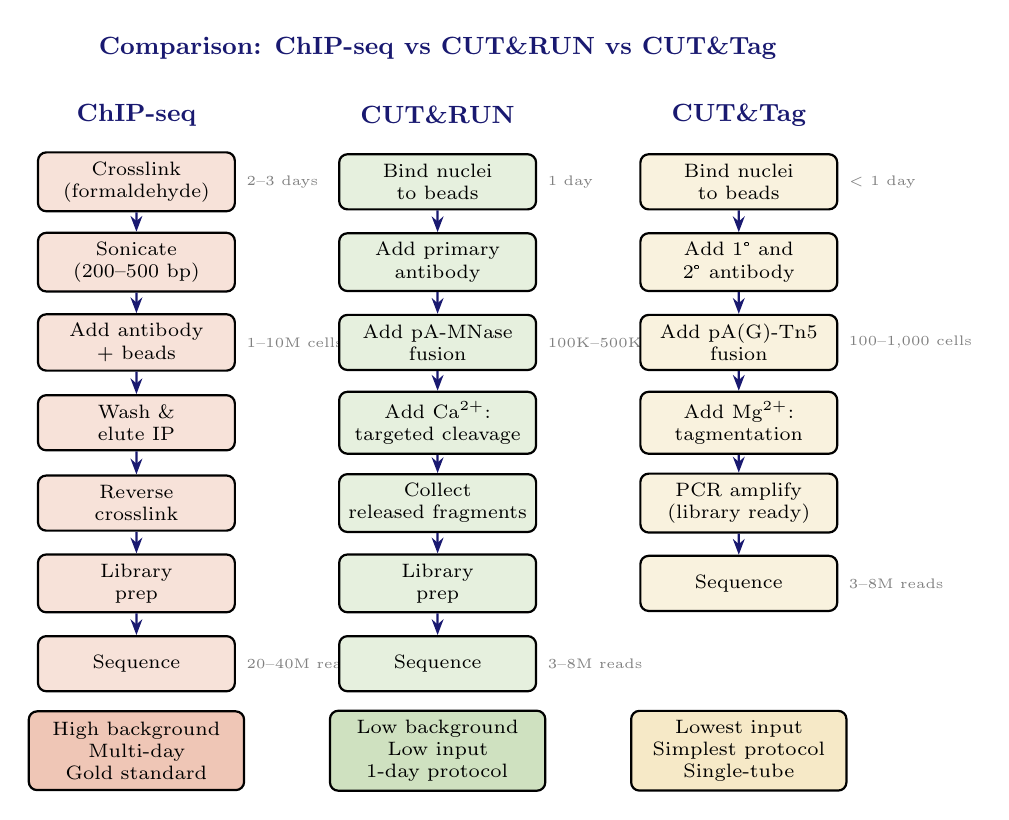
\begin{tikzpicture}[
  scale=0.85,
  node distance=0.8cm,
  box/.style={draw, rounded corners=3pt, thick, minimum width=2.5cm, minimum height=0.7cm, align=center, font=\scriptsize},
  arrow/.style={-{Stealth[length=2mm]}, thick, MidnightBlue},
  method/.style={font=\small\bfseries, MidnightBlue},
  labelstep/.style={font=\tiny, gray}
]

% Title
\node[font=\bfseries\small, MidnightBlue] at (6, 11.5) {Comparison: ChIP-seq vs CUT\&RUN vs CUT\&Tag};

% === ChIP-seq column ===
\node[method] at (1.5, 10.5) {ChIP-seq};

\node[box, fill=BrickRed!10] (cs1) at (1.5, 9.5) {Crosslink\\(formaldehyde)};
\node[box, fill=BrickRed!10] (cs2) at (1.5, 8.3) {Sonicate\\(200--500 bp)};
\node[box, fill=BrickRed!10] (cs3) at (1.5, 7.1) {Add antibody\\+ beads};
\node[box, fill=BrickRed!10] (cs4) at (1.5, 5.9) {Wash \&\\elute IP};
\node[box, fill=BrickRed!10] (cs5) at (1.5, 4.7) {Reverse\\crosslink};
\node[box, fill=BrickRed!10] (cs6) at (1.5, 3.5) {Library\\prep};
\node[box, fill=BrickRed!10] (cs7) at (1.5, 2.3) {Sequence};

\draw[arrow] (cs1) -- (cs2);
\draw[arrow] (cs2) -- (cs3);
\draw[arrow] (cs3) -- (cs4);
\draw[arrow] (cs4) -- (cs5);
\draw[arrow] (cs5) -- (cs6);
\draw[arrow] (cs6) -- (cs7);

\node[labelstep, right] at (3.0, 9.5) {2--3 days};
\node[labelstep, right] at (3.0, 7.1) {1--10M cells};
\node[labelstep, right] at (3.0, 2.3) {20--40M reads};

% === CUT&RUN column ===
\node[method] at (6, 10.5) {CUT\&RUN};

\node[box, fill=OliveGreen!10] (cr1) at (6, 9.5) {Bind nuclei\\to beads};
\node[box, fill=OliveGreen!10] (cr2) at (6, 8.3) {Add primary\\antibody};
\node[box, fill=OliveGreen!10] (cr3) at (6, 7.1) {Add pA-MNase\\fusion};
\node[box, fill=OliveGreen!10] (cr4) at (6, 5.9) {Add Ca$^{2+}$:\\targeted cleavage};
\node[box, fill=OliveGreen!10] (cr5) at (6, 4.7) {Collect\\released fragments};
\node[box, fill=OliveGreen!10] (cr6) at (6, 3.5) {Library\\prep};
\node[box, fill=OliveGreen!10] (cr7) at (6, 2.3) {Sequence};

\draw[arrow] (cr1) -- (cr2);
\draw[arrow] (cr2) -- (cr3);
\draw[arrow] (cr3) -- (cr4);
\draw[arrow] (cr4) -- (cr5);
\draw[arrow] (cr5) -- (cr6);
\draw[arrow] (cr6) -- (cr7);

\node[labelstep, right] at (7.5, 9.5) {1 day};
\node[labelstep, right] at (7.5, 7.1) {100K--500K cells};
\node[labelstep, right] at (7.5, 2.3) {3--8M reads};

% === CUT&Tag column ===
\node[method] at (10.5, 10.5) {CUT\&Tag};

\node[box, fill=Goldenrod!15] (ct1) at (10.5, 9.5) {Bind nuclei\\to beads};
\node[box, fill=Goldenrod!15] (ct2) at (10.5, 8.3) {Add 1\textdegree{} and\\2\textdegree{} antibody};
\node[box, fill=Goldenrod!15] (ct3) at (10.5, 7.1) {Add pA(G)-Tn5\\fusion};
\node[box, fill=Goldenrod!15] (ct4) at (10.5, 5.9) {Add Mg$^{2+}$:\\tagmentation};
\node[box, fill=Goldenrod!15] (ct5) at (10.5, 4.7) {PCR amplify\\(library ready)};
\node[box, fill=Goldenrod!15] (ct7) at (10.5, 3.5) {Sequence};

\draw[arrow] (ct1) -- (ct2);
\draw[arrow] (ct2) -- (ct3);
\draw[arrow] (ct3) -- (ct4);
\draw[arrow] (ct4) -- (ct5);
\draw[arrow] (ct5) -- (ct7);

\node[labelstep, right] at (12, 9.5) {$<$ 1 day};
\node[labelstep, right] at (12, 7.1) {100--1,000 cells};
\node[labelstep, right] at (12, 3.5) {3--8M reads};

% Summary boxes at bottom
\node[box, fill=BrickRed!20, text width=2.5cm, minimum height=1cm] at (1.5, 1.0) {High background\\Multi-day\\Gold standard};
\node[box, fill=OliveGreen!20, text width=2.5cm, minimum height=1cm] at (6, 1.0) {Low background\\Low input\\1-day protocol};
\node[box, fill=Goldenrod!25, text width=2.5cm, minimum height=1cm] at (10.5, 1.0) {Lowest input\\Simplest protocol\\Single-tube};

\end{tikzpicture}
\caption[Comparison of ChIP-seq, CUT\&RUN, and CUT\&Tag workflows.]{Side-by-side comparison of ChIP-seq, CUT\&RUN, and CUT\&Tag workflows. CUT\&RUN and CUT\&Tag progressively simplify the protocol, reduce input requirements, lower background, and decrease the sequencing depth needed. CUT\&Tag is the simplest, requiring as few as 100--1,000 cells and producing sequencing-ready libraries in a single tube.}
\label{fig:histones:comparison}
\end{figure}

\subsection{Advantages and Limitations of CUT\&Tag}
\label{subsec:histones:cuttag-advantages}

\textbf{Advantages:}
\begin{itemize}[itemsep=2pt]
  \item Works with as few as \textbf{100--1,000 cells} (or even single cells).
  \item \textbf{Single-tube protocol:} no library preparation step---tagmentation directly inserts adapters.
  \item \textbf{Excellent signal-to-noise ratio:} very low background because only target-proximal DNA is tagmented.
  \item \textbf{Low sequencing cost:} 3--8 million reads are sufficient for most histone marks.
  \item \textbf{Fast:} can be completed in half a day.
  \item \textbf{No crosslinking or sonication required.}
\end{itemize}

\textbf{Limitations:}
\begin{itemize}[itemsep=2pt]
  \item Works best for \textbf{abundant histone marks} (H3K27me3, H3K4me3, H3K27ac). Less reliable for transcription factors with small footprints and low abundance.
  \item Requires a \textbf{secondary antibody} (or Protein A/G-Tn5 that binds the primary directly).
  \item The pAG-Tn5 reagent may not be commercially available from all vendors; some labs produce it in-house.
  \item Some bias from Tn5 sequence preferences (similar to ATAC-seq).
\end{itemize}

\begin{tipbox}
For most new histone modification profiling experiments, CUT\&Tag is the recommended starting point. It offers the simplest protocol, lowest input, and lowest cost. Reserve ChIP-seq for situations requiring ENCODE-standard comparability, for transcription factors that fail with CUT\&Tag, or when large existing ChIP-seq datasets provide better statistical frameworks.
\end{tipbox}

%% ============================================================
\section{Single-Cell CUT\&Tag}
\label{sec:histones:sc-cuttag}

Single-cell CUT\&Tag enables profiling of histone modifications in individual cells. Approaches include:

\begin{itemize}[itemsep=3pt]
  \item \textbf{Droplet-based scCUT\&Tag:} Nuclei are tagmented in bulk, then single nuclei are encapsulated in droplets (10x Genomics or similar) for barcoding, analogous to scATAC-seq.
  \item \textbf{Plate-based scCUT\&Tag:} Individual cells or nuclei are sorted into 96/384-well plates, and the CUT\&Tag reaction is performed in each well with unique index primers.
  \item \textbf{Multi-CUT\&Tag:} Profiling multiple histone marks simultaneously in the same cell using different antibody--barcode combinations.
\end{itemize}

scCUT\&Tag data shares the extreme sparsity challenges of scATAC-seq and uses similar computational approaches (LSI, clustering, pseudo-bulk analysis).

%% ============================================================
\section{PLAC-seq and HiChIP}
\label{sec:histones:plac-hichip}

PLAC-seq (Proximity Ligation-Assisted ChIP-seq) and HiChIP combine chromatin immunoprecipitation with proximity ligation to map chromatin interactions at sites bound by a specific protein or bearing a specific histone mark:

\begin{itemize}[itemsep=3pt]
  \item \textbf{HiChIP:} Cells are crosslinked, chromatin is digested with a restriction enzyme, and proximity ligation joins nearby fragments. The ligated chromatin is then immunoprecipitated with an antibody (e.g., anti-H3K27ac) and sequenced.
  \item \textbf{PLAC-seq:} Similar to HiChIP but with ChIP performed before proximity ligation.
  \item \textbf{Application:} H3K27ac HiChIP is widely used to map \textbf{active enhancer--promoter loops}, providing direct evidence for which enhancers regulate which genes.
  \item \textbf{Advantage over Hi-C:} By enriching for contacts at active regulatory elements, HiChIP requires far less sequencing depth than genome-wide Hi-C to detect enhancer--promoter interactions.
\end{itemize}

%% ============================================================
\section{RNA--Protein Interaction Methods}
\label{sec:histones:clip}

\subsection{CLIP-seq / eCLIP}
\label{subsec:histones:clip}

Cross-Linking and Immunoprecipitation followed by sequencing (CLIP-seq) maps the binding sites of \textbf{RNA-binding proteins (RBPs)} on RNA:

\begin{enumerate}[itemsep=2pt]
  \item UV crosslink cells (254 nm) to covalently link RBPs to bound RNA.
  \item Lyse cells and fragment RNA (RNase treatment).
  \item Immunoprecipitate with an anti-RBP antibody.
  \item Ligate adapters to RNA fragments.
  \item Reverse transcribe, amplify, and sequence.
\end{enumerate}

Key variants:
\begin{itemize}[itemsep=2pt]
  \item \textbf{iCLIP} (individual-nucleotide resolution CLIP): uses a circularisation step to capture cDNA truncation sites, providing nucleotide-resolution binding sites.
  \item \textbf{eCLIP} (enhanced CLIP): the ENCODE standard method. Includes size-matched input controls and an optimised protocol that improves library complexity and reduces artefacts. ENCODE has generated eCLIP datasets for $>$150 RBPs across multiple cell lines.
  \item \textbf{irCLIP} (infrared CLIP): uses infrared-labelled adapters for visualisation and optimised efficiency.
\end{itemize}

\subsection{RIP-seq}
\label{subsec:histones:rip}

RNA Immunoprecipitation sequencing (RIP-seq) is a simpler alternative to CLIP-seq. Cells are lysed, and an antibody against the RBP is used to immunoprecipitate the protein along with associated RNA, which is then sequenced. Unlike CLIP, RIP-seq does not use UV crosslinking, which makes it simpler but also means that some interactions may be lost or artefactual (due to post-lysis reassociation). RIP-seq provides transcript-level rather than nucleotide-level resolution.

\subsection{DAP-seq}
\label{subsec:histones:dap}

DNA Affinity Purification sequencing (DAP-seq) is an \textit{in vitro} method for mapping transcription factor binding sites. Purified TF protein is incubated with naked genomic DNA (no chromatin context), and bound fragments are captured and sequenced. DAP-seq is widely used in plant genomics, where ChIP-grade antibodies are often unavailable, and has been applied to survey the binding specificities of hundreds of plant TFs.

%% ============================================================
\section{Bioinformatics Workflow for ChIP-seq/CUT\&Tag}
\label{sec:histones:bioinformatics}

\subsection{Analysis Overview}
\label{subsec:histones:analysis-overview}

The core bioinformatics pipeline for ChIP-seq, CUT\&RUN, and CUT\&Tag data follows a common structure, with minor differences in parameter settings:

\begin{enumerate}[itemsep=2pt]
  \item \textbf{Quality control:} FastQC, MultiQC.
  \item \textbf{Trimming:} Trim Galore or fastp (adapter removal).
  \item \textbf{Alignment:} Bowtie2 (SE or PE). Use \texttt{--very-sensitive} mode. For CUT\&Tag, use \texttt{--very-sensitive --no-mixed --no-discordant -X 700}.
  \item \textbf{Filtering:} Remove duplicates, low-quality reads (MAPQ $<$ 30), and reads in blacklist regions.
  \item \textbf{Peak calling:}
    \begin{itemize}[itemsep=1pt]
      \item \textbf{Sharp/narrow peaks} (H3K4me3, H3K27ac, TFs): MACS2 default settings.
      \item \textbf{Broad peaks} (H3K27me3, H3K9me3, H3K36me3): MACS2 with \texttt{--broad} flag, or SICER2/epic2.
    \end{itemize}
  \item \textbf{Reproducibility:} IDR (Irreproducibility Discovery Rate) to assess peak reproducibility across replicates.
  \item \textbf{Differential binding:} DiffBind or MAnorm2.
  \item \textbf{Visualisation:} deepTools (computeMatrix, plotHeatmap, plotProfile), IGV.
  \item \textbf{Chromatin state segmentation:} ChromHMM (when profiling multiple marks).
\end{enumerate}

\subsubsection{Quality Metrics}

\begin{itemize}[itemsep=2pt]
  \item \textbf{FRiP (Fraction of Reads in Peaks):} ENCODE minimum is 1\% for broad marks and 1\% for narrow marks, though good experiments typically achieve 5--30\%.
  \item \textbf{Cross-correlation (strand-shift) analysis:} Plots the Pearson correlation between read density on the + and $-$ strands as a function of strand shift. A clear peak at the fragment length indicates successful enrichment. Metrics include NSC (Normalised Strand Coefficient) and RSC (Relative Strand Correlation).
  \item \textbf{IDR (Irreproducibility Discovery Rate):} Measures concordance between biological replicates. Peaks with IDR $<$ 0.05 are considered reproducible.
  \item \textbf{Library complexity:} NRF (Non-Redundant Fraction), PBC1, PBC2 metrics from ENCODE.
\end{itemize}

\subsubsection{ChIP Enrichment Statistics in Detail}
\label{subsubsec:histones:enrichment-stats}

The quality of a ChIP-seq or CUT\&Tag experiment is determined by the degree of enrichment above background. Three key metrics---FRiP, NSC, and RSC---quantify this enrichment from complementary perspectives.

\textbf{FRiP (Fraction of Reads in Peaks).} FRiP measures the proportion of all mapped reads that fall within called peaks:
\begin{equation}
\label{eq:histones:frip}
\text{FRiP} = \frac{\text{Number of reads in peaks}}{\text{Total number of mapped reads}}
\end{equation}

ENCODE has established the following FRiP guidelines:
\begin{itemize}[itemsep=2pt]
  \item \textbf{Sharp/narrow marks} (H3K4me3, H3K27ac, TFs): FRiP $> 5\%$ is acceptable; FRiP $> 10\%$ indicates a high-quality experiment. Top-performing experiments can achieve FRiP $> 30\%$.
  \item \textbf{Broad marks} (H3K27me3, H3K9me3, H3K36me3): FRiP $> 1\%$ is the minimum ENCODE threshold. Because broad marks span large genomic domains, a lower FRiP can still represent genuine enrichment. Values of 5--15\% are typical for well-performing experiments.
  \item FRiP is sensitive to peak calling parameters: more lenient thresholds inflate FRiP. Always report the peak caller and parameters used alongside FRiP values.
\end{itemize}

\textbf{Cross-Correlation Analysis: NSC and RSC.} The strand cross-correlation analysis exploits the directional asymmetry of ChIP-seq fragments. In a successful ChIP experiment, reads on the forward ($+$) strand are shifted upstream of the true binding site, while reads on the reverse ($-$) strand are shifted downstream, by a distance equal to the fragment length. Computing the Pearson correlation between $+$ strand and $-$ strand read density as a function of strand shift $d$ produces a cross-correlation profile with:

\begin{itemize}[itemsep=2pt]
  \item A peak at $d = \text{fragment length}$ (the true enrichment signal).
  \item A ``phantom'' peak at $d = \text{read length}$ (an artefact of mappability).
\end{itemize}

The two quality metrics derived from this profile are:
\begin{align}
\label{eq:histones:nsc}
\text{NSC (Normalised Strand Coefficient)} &= \frac{CC_{\text{fragment}}}{CC_{\min}} \\[6pt]
\label{eq:histones:rsc}
\text{RSC (Relative Strand Coefficient)} &= \frac{CC_{\text{fragment}} - CC_{\min}}{CC_{\text{phantom}} - CC_{\min}}
\end{align}
where $CC_{\text{fragment}}$ is the cross-correlation at the fragment-length shift, $CC_{\text{phantom}}$ is the cross-correlation at the read-length shift, and $CC_{\min}$ is the minimum cross-correlation value.

ENCODE thresholds:
\begin{itemize}[itemsep=2pt]
  \item \textbf{NSC $\geq$ 1.05} and \textbf{RSC $\geq$ 0.8}: acceptable quality.
  \item \textbf{NSC $\geq$ 1.1} and \textbf{RSC $\geq$ 1.0}: high quality.
  \item NSC or RSC values near 1.0 suggest weak enrichment or failed ChIP.
\end{itemize}

These metrics are computed by the \software{phantompeakqualtools} R package (also called \software{SPP}), which is integrated into the ENCODE pipeline and \software{nf-core/chipseq}.

\subsubsection{Spike-in Normalisation for Quantitative Comparisons}
\label{subsubsec:histones:spikein}

Standard ChIP-seq normalisation methods (e.g., reads per million, RPGC) assume that the total amount of the target modification is approximately constant across samples. This assumption fails in experimental settings where the modification undergoes \textbf{global changes}---for example, when comparing cells treated with an HDAC inhibitor (global increase in acetylation) to untreated cells, or when studying H3K27me3 loss after \gene{EZH2} knockout.

\textbf{The spike-in approach.} To enable quantitative comparisons when global histone modification levels change, a known amount of chromatin from a different species is added to each sample before immunoprecipitation:

\begin{enumerate}[itemsep=2pt]
  \item Add a fixed amount of \species{Drosophila melanogaster} chromatin (typically 1--5\% of the total chromatin mass) to each human/mouse sample prior to the ChIP step.
  \item Perform ChIP using an antibody that recognises both the human/mouse target and the \species{Drosophila} ortholog (e.g., anti-H3K27me3 recognises the mark in both species), or add a second antibody against a \species{Drosophila}-specific histone variant (anti-H2Av).
  \item After sequencing, align reads to a combined human/mouse + \species{Drosophila} reference genome.
  \item Use the number of reads mapping to the \species{Drosophila} genome as a normalisation factor.
\end{enumerate}

\textbf{The scaling formula.} For sample $i$, the spike-in scaling factor is:
\begin{equation}
\label{eq:histones:spikein-scale}
\text{scale}_i = \frac{\text{median}_{j}(\text{spike}_j)}{\text{spike}_i}
\end{equation}
where $\text{spike}_i$ is the number of reads mapping to the \species{Drosophila} genome in sample $i$, and the median is taken across all samples in the experiment. Multiplying the human/mouse read counts by $\text{scale}_i$ adjusts for differences in ChIP efficiency and global modification levels.

\begin{warningbox}
Spike-in normalisation requires careful experimental execution. The \species{Drosophila} chromatin must be added at a consistent ratio before the immunoprecipitation step---not after. Variation in the spike-in amount across samples introduces normalisation artefacts. Additionally, the spike-in reads should constitute 1--10\% of the total reads; too few spike-in reads lead to noisy normalisation, while too many waste sequencing capacity on non-target reads. Active Motif and EpiCypher offer commercial spike-in kits with calibrated standards.
\end{warningbox}

\subsection{Snakemake Workflow}
\label{subsec:histones:snakemake}

\begin{lstlisting}[language=Python, caption={Snakemake workflow for ChIP-seq/CUT\&Tag analysis.}, label={lst:histones:snakemake}]
# Snakefile for ChIP-seq / CUT&Tag analysis
configfile: "config.yaml"

SAMPLES = config["samples"]        # Dict: sample -> {mark, condition}
CONTROLS = config["controls"]      # Dict: sample -> input_control
GENOME = config["genome_index"]    # Bowtie2 index prefix
BLACKLIST = config["blacklist"]
EFFECTIVE_GENOME = config["effective_genome_size"]

rule all:
    input:
        "results/multiqc/multiqc_report.html",
        expand("results/peaks/{sample}_peaks.broadPeak",
               sample=[s for s in SAMPLES
                       if SAMPLES[s]["mark"] in
                       ["H3K27me3","H3K9me3","H3K36me3"]]),
        expand("results/peaks/{sample}_peaks.narrowPeak",
               sample=[s for s in SAMPLES
                       if SAMPLES[s]["mark"] in
                       ["H3K4me3","H3K27ac"]]),
        expand("results/bigwig/{sample}.bw", sample=SAMPLES),
        "results/deeptools/heatmap_TSS.pdf",
        "results/diffbind/differential_binding.tsv",
        "results/chromhmm/chromatin_states.bed"

rule trim_reads:
    input:
        r1 = "raw_data/{sample}_R1.fastq.gz",
        r2 = "raw_data/{sample}_R2.fastq.gz"
    output:
        r1 = "results/trimmed/{sample}_R1_val_1.fq.gz",
        r2 = "results/trimmed/{sample}_R2_val_2.fq.gz"
    threads: 4
    conda: "envs/trim_galore.yaml"
    shell:
        """
        trim_galore --paired --cores {threads} \
            --output_dir results/trimmed \
            {input.r1} {input.r2}
        """

rule bowtie2_align:
    input:
        r1 = "results/trimmed/{sample}_R1_val_1.fq.gz",
        r2 = "results/trimmed/{sample}_R2_val_2.fq.gz"
    output:
        bam = "results/aligned/{sample}.bam",
        bai = "results/aligned/{sample}.bam.bai"
    threads: 12
    resources:
        mem_mb = 16000
    conda: "envs/bowtie2.yaml"
    shell:
        """
        bowtie2 --very-sensitive --no-mixed \
            --no-discordant -X 700 \
            --threads {threads} \
            -x {GENOME} \
            -1 {input.r1} -2 {input.r2} \
        | samtools sort -@ {threads} -O bam -o - \
        | samtools markdup -r -@ {threads} - {output.bam}
        samtools index {output.bam}
        """

rule filter_bam:
    input:
        bam = "results/aligned/{sample}.bam",
        bai = "results/aligned/{sample}.bam.bai"
    output:
        bam = "results/filtered/{sample}_filtered.bam",
        bai = "results/filtered/{sample}_filtered.bam.bai"
    params:
        blacklist = BLACKLIST
    conda: "envs/samtools.yaml"
    shell:
        """
        samtools view -b -f 2 -q 30 {input.bam} \
            | bedtools intersect -v -abam stdin \
                -b {params.blacklist} \
            > {output.bam}
        samtools index {output.bam}
        """

rule macs2_narrow:
    input:
        treatment = "results/filtered/{sample}_filtered.bam",
        control = lambda wc: "results/filtered/"
                  + CONTROLS[wc.sample] + "_filtered.bam"
    output:
        peaks = "results/peaks/{sample}_peaks.narrowPeak"
    params:
        name = "{sample}",
        gs = EFFECTIVE_GENOME
    conda: "envs/macs2.yaml"
    shell:
        """
        macs2 callpeak -t {input.treatment} \
            -c {input.control} \
            -f BAMPE -g {params.gs} \
            -n {params.name} --outdir results/peaks \
            -q 0.01
        """

rule macs2_broad:
    input:
        treatment = "results/filtered/{sample}_filtered.bam",
        control = lambda wc: "results/filtered/"
                  + CONTROLS[wc.sample] + "_filtered.bam"
    output:
        peaks = "results/peaks/{sample}_peaks.broadPeak"
    params:
        name = "{sample}",
        gs = EFFECTIVE_GENOME
    conda: "envs/macs2.yaml"
    shell:
        """
        macs2 callpeak -t {input.treatment} \
            -c {input.control} \
            -f BAMPE -g {params.gs} \
            -n {params.name} --outdir results/peaks \
            --broad --broad-cutoff 0.05
        """

rule make_bigwig:
    input:
        bam = "results/filtered/{sample}_filtered.bam",
        bai = "results/filtered/{sample}_filtered.bam.bai"
    output:
        bw = "results/bigwig/{sample}.bw"
    threads: 4
    params:
        gs = EFFECTIVE_GENOME
    conda: "envs/deeptools.yaml"
    shell:
        """
        bamCoverage -b {input.bam} -o {output.bw} \
            --binSize 10 --normalizeUsing RPGC \
            --effectiveGenomeSize {params.gs} \
            -p {threads} --extendReads
        """

rule deeptools_heatmap:
    input:
        bw = expand("results/bigwig/{sample}.bw",
                     sample=SAMPLES),
        bed = config["tss_bed"]
    output:
        matrix = "results/deeptools/matrix_TSS.gz",
        heatmap = "results/deeptools/heatmap_TSS.pdf",
        profile = "results/deeptools/profile_TSS.pdf"
    threads: 8
    conda: "envs/deeptools.yaml"
    shell:
        """
        computeMatrix reference-point \
            -S {input.bw} -R {input.bed} \
            --referencePoint TSS \
            -b 3000 -a 3000 \
            -p {threads} -o {output.matrix}

        plotHeatmap -m {output.matrix} \
            -o {output.heatmap} \
            --colorMap RdBu_r \
            --whatToShow 'heatmap and colorbar'

        plotProfile -m {output.matrix} \
            -o {output.profile} \
            --perGroup
        """

rule diffbind:
    input:
        peaks = expand("results/peaks/{sample}_peaks.narrowPeak",
                       sample=SAMPLES),
        bams = expand("results/filtered/{sample}_filtered.bam",
                      sample=SAMPLES)
    output:
        "results/diffbind/differential_binding.tsv"
    conda: "envs/diffbind.yaml"
    script:
        "scripts/run_diffbind.R"

rule chromhmm:
    input:
        bams = expand("results/filtered/{sample}_filtered.bam",
                      sample=SAMPLES)
    output:
        "results/chromhmm/chromatin_states.bed"
    conda: "envs/chromhmm.yaml"
    script:
        "scripts/run_chromhmm.sh"

rule multiqc:
    input:
        expand("results/aligned/{sample}.bam", sample=SAMPLES)
    output:
        "results/multiqc/multiqc_report.html"
    conda: "envs/multiqc.yaml"
    shell:
        "multiqc results/ -o results/multiqc --force"
\end{lstlisting}

\subsection{Nextflow Workflow}
\label{subsec:histones:nextflow}

\begin{lstlisting}[language=Java, caption={Nextflow DSL2 workflow for ChIP-seq/CUT\&Tag analysis.}, label={lst:histones:nextflow}]
#!/usr/bin/env nextflow
nextflow.enable.dsl=2

params.reads          = "raw_data/*_R{1,2}.fastq.gz"
params.genome_index   = "reference/genome"
params.genome_fasta   = "reference/genome.fa"
params.blacklist      = "reference/blacklist.bed"
params.effective_size = "2.7e9"
params.tss_bed        = "reference/tss_regions.bed"
params.sample_sheet   = "sample_sheet.csv"
params.outdir         = "results"

process TRIM_READS {
    tag "$sample_id"
    cpus 4
    publishDir "${params.outdir}/trimmed", mode: 'copy'

    input:
    tuple val(sample_id), path(reads)

    output:
    tuple val(sample_id), path("*_val_{1,2}.fq.gz"),
                                             emit: trimmed
    path "*_trimming_report.txt",            emit: reports

    script:
    """
    trim_galore --paired --cores ${task.cpus} \
        ${reads[0]} ${reads[1]}
    """
}

process BOWTIE2_ALIGN {
    tag "$sample_id"
    cpus 12
    memory '16 GB'
    publishDir "${params.outdir}/aligned", mode: 'copy'

    input:
    tuple val(sample_id), path(reads)

    output:
    tuple val(sample_id),
          path("${sample_id}.bam"),
          path("${sample_id}.bam.bai"),      emit: bam

    script:
    """
    bowtie2 --very-sensitive --no-mixed \
        --no-discordant -X 700 \
        --threads ${task.cpus} \
        -x ${params.genome_index} \
        -1 ${reads[0]} -2 ${reads[1]} \
    | samtools sort -@ ${task.cpus} -O bam \
    | samtools markdup -r -@ ${task.cpus} - \
        ${sample_id}.bam
    samtools index ${sample_id}.bam
    """
}

process FILTER_BAM {
    tag "$sample_id"
    publishDir "${params.outdir}/filtered", mode: 'copy'

    input:
    tuple val(sample_id), path(bam), path(bai)

    output:
    tuple val(sample_id),
          path("${sample_id}_filt.bam"),
          path("${sample_id}_filt.bam.bai"), emit: bam

    script:
    """
    samtools view -b -f 2 -q 30 ${bam} \
        | bedtools intersect -v -abam stdin \
            -b ${params.blacklist} \
        > ${sample_id}_filt.bam
    samtools index ${sample_id}_filt.bam
    """
}

process CALL_PEAKS_NARROW {
    tag "$sample_id"
    publishDir "${params.outdir}/peaks", mode: 'copy'

    input:
    tuple val(sample_id), path(treat_bam), path(treat_bai)
    tuple val(control_id), path(ctrl_bam), path(ctrl_bai)

    output:
    tuple val(sample_id),
          path("${sample_id}_peaks.narrowPeak"),
                                             emit: peaks

    script:
    """
    macs2 callpeak -t ${treat_bam} \
        -c ${ctrl_bam} -f BAMPE \
        -g ${params.effective_size} \
        -n ${sample_id} -q 0.01
    """
}

process CALL_PEAKS_BROAD {
    tag "$sample_id"
    publishDir "${params.outdir}/peaks", mode: 'copy'

    input:
    tuple val(sample_id), path(treat_bam), path(treat_bai)
    tuple val(control_id), path(ctrl_bam), path(ctrl_bai)

    output:
    tuple val(sample_id),
          path("${sample_id}_peaks.broadPeak"),
                                             emit: peaks

    script:
    """
    macs2 callpeak -t ${treat_bam} \
        -c ${ctrl_bam} -f BAMPE \
        -g ${params.effective_size} \
        -n ${sample_id} \
        --broad --broad-cutoff 0.05
    """
}

process BIGWIG {
    tag "$sample_id"
    cpus 4
    publishDir "${params.outdir}/bigwig", mode: 'copy'

    input:
    tuple val(sample_id), path(bam), path(bai)

    output:
    tuple val(sample_id), path("${sample_id}.bw"),
                                             emit: bigwig

    script:
    """
    bamCoverage -b ${bam} -o ${sample_id}.bw \
        --binSize 10 --normalizeUsing RPGC \
        --effectiveGenomeSize ${params.effective_size} \
        -p ${task.cpus} --extendReads
    """
}

process DEEPTOOLS_HEATMAP {
    cpus 8
    publishDir "${params.outdir}/deeptools", mode: 'copy'

    input:
    path bigwigs
    path tss_bed

    output:
    path "heatmap_TSS.pdf"
    path "profile_TSS.pdf"

    script:
    """
    computeMatrix reference-point \
        -S ${bigwigs} -R ${tss_bed} \
        --referencePoint TSS \
        -b 3000 -a 3000 \
        -p ${task.cpus} -o matrix_TSS.gz

    plotHeatmap -m matrix_TSS.gz \
        -o heatmap_TSS.pdf \
        --colorMap RdBu_r

    plotProfile -m matrix_TSS.gz \
        -o profile_TSS.pdf --perGroup
    """
}

// Main workflow
workflow {
    reads_ch = Channel
        .fromFilePairs(params.reads,
                       checkIfExists: true)

    TRIM_READS(reads_ch)
    BOWTIE2_ALIGN(TRIM_READS.out.trimmed)
    FILTER_BAM(BOWTIE2_ALIGN.out.bam)
    BIGWIG(FILTER_BAM.out.bam)

    DEEPTOOLS_HEATMAP(
        BIGWIG.out.bigwig.map{ it[1] }.collect(),
        file(params.tss_bed)
    )
}
\end{lstlisting}

\begin{tipbox}
The nf-core community provides \software{nf-core/chipseq} for ChIP-seq data and \software{nf-core/cutandrun} for CUT\&RUN/CUT\&Tag data. Both pipelines handle alignment, filtering, peak calling, QC, and visualisation with sensible defaults and extensive documentation. They support both narrow and broad peak calling modes and include IDR analysis for replicate concordance.
\end{tipbox}

\subsection{ChromHMM: Chromatin State Segmentation}
\label{subsec:histones:chromhmm}

When multiple histone marks have been profiled in the same cell type, \textbf{ChromHMM} uses a multivariate hidden Markov model to segment the genome into discrete chromatin states:

\begin{enumerate}[itemsep=2pt]
  \item \textbf{Binarise:} Convert each histone mark's signal into binary (present/absent) calls in 200\basepair{} genomic bins.
  \item \textbf{Learn model:} Train an HMM with a user-specified number of states (typically 15--18). The model learns the emission probabilities (which combinations of marks define each state) and transition probabilities (how states change along the genome).
  \item \textbf{Segment:} Apply the trained model to assign each 200\basepair{} bin to a chromatin state.
  \item \textbf{Annotate:} Compare the learned states to known genomic features (TSSs, gene bodies, enhancers, heterochromatin) to assign biological labels.
\end{enumerate}

\begin{keyconcept}[title={Typical ChromHMM States (15-State Model)}]
\begin{itemize}[itemsep=1pt]
  \item States 1--3: Active TSS and flanking regions (H3K4me3, H3K27ac)
  \item States 4--5: Transcription (H3K36me3)
  \item States 6--7: Active enhancers (H3K4me1, H3K27ac)
  \item States 8--9: Zinc finger genes and repeats (H3K9me3, H3K36me3)
  \item States 10--11: Poised/bivalent elements (H3K4me1/me3, H3K27me3)
  \item States 12--13: Polycomb repressed (H3K27me3)
  \item States 14--15: Quiescent/heterochromatin (H3K9me3 or no marks)
\end{itemize}
\end{keyconcept}

\subsubsection{ChromHMM Emission and Transition Model}
\label{subsubsec:histones:chromhmm-model}

ChromHMM formalises the combinatorial histone code as a \textbf{multivariate hidden Markov model (HMM)}. Understanding the mathematical framework clarifies how chromatin states are learned and why the resulting annotations are biologically meaningful.

\textbf{Hidden states and observations.} The genome is divided into fixed-size bins (typically 200\basepair{}). At each bin $t$ along the genome, the hidden state $q_t \in \{1, 2, \ldots, K\}$ represents the unknown chromatin state, and the observation $\mathbf{o}_t = (o_{t,1}, o_{t,2}, \ldots, o_{t,M})$ is a binary vector indicating the presence (1) or absence (0) of each of $M$ histone marks. With six marks (the ``core six''), each bin has a 6-dimensional binary observation vector, yielding $2^6 = 64$ possible observation patterns.

\textbf{Emission probabilities.} Each chromatin state $k$ has an associated \textbf{emission probability matrix} that defines how likely each histone mark is to be observed when the genome is in state $k$. Assuming conditional independence of marks given the state (a key simplifying assumption), the emission probability for observing pattern $\mathbf{o}_t$ in state $k$ is:
\begin{equation}
\label{eq:histones:chromhmm-emission}
P(\mathbf{o}_t \mid q_t = k) = \prod_{m=1}^{M} p_{k,m}^{\,o_{t,m}} \,(1 - p_{k,m})^{1 - o_{t,m}}
\end{equation}
where $p_{k,m}$ is the probability of observing mark $m$ in state $k$. The emission matrix $\mathbf{P} = [p_{k,m}]_{K \times M}$ is typically visualised as a heatmap, where each row is a state and each column is a mark. For example, the ``Active TSS'' state has high emission probabilities for H3K4me3 and H3K27ac but low probabilities for H3K27me3.

\textbf{Transition probabilities.} The \textbf{transition matrix} $\mathbf{A} = [a_{k,l}]_{K \times K}$ specifies the probability of transitioning from state $k$ to state $l$ between adjacent bins:
\begin{equation}
\label{eq:histones:chromhmm-transition}
a_{k,l} = P(q_{t+1} = l \mid q_t = k)
\end{equation}
with $\sum_{l=1}^{K} a_{k,l} = 1$ for all $k$. The transition matrix encodes the spatial organisation of chromatin states. For example, the ``Active TSS'' state has a high transition probability to the ``Flanking TSS'' state and a low probability of transitioning directly to ``Heterochromatin.''

\textbf{Training with Baum--Welch.} The emission and transition parameters are learned from the data using the \textbf{Baum--Welch algorithm} (a special case of expectation-maximisation for HMMs):
\begin{enumerate}[itemsep=2pt]
  \item \textbf{Initialisation:} Randomly initialise the emission matrix $\mathbf{P}$, transition matrix $\mathbf{A}$, and initial state distribution $\boldsymbol{\pi}$.
  \item \textbf{E-step (Forward--Backward):} Compute the posterior probability $\gamma_t(k) = P(q_t = k \mid \mathbf{O})$ that each bin is in each state, given the full observation sequence $\mathbf{O}$ and current parameters.
  \item \textbf{M-step:} Update the parameters to maximise the expected log-likelihood:
  \begin{itemize}[itemsep=1pt]
    \item $\hat{p}_{k,m} = \sum_t \gamma_t(k) \cdot o_{t,m} \;/\; \sum_t \gamma_t(k)$
    \item $\hat{a}_{k,l} = \sum_t \xi_t(k,l) \;/\; \sum_t \gamma_t(k)$
  \end{itemize}
  where $\xi_t(k,l) = P(q_t = k, q_{t+1} = l \mid \mathbf{O})$.
  \item \textbf{Iterate} E- and M-steps until convergence.
\end{enumerate}

\textbf{Decoding with Viterbi.} Once the model is trained, the \textbf{Viterbi algorithm} finds the most probable sequence of hidden states (chromatin state assignment) for each chromosome:
\begin{equation}
\label{eq:histones:chromhmm-viterbi}
\hat{\mathbf{q}} = \arg\max_{\mathbf{q}} P(\mathbf{q} \mid \mathbf{O},\; \mathbf{A},\; \mathbf{P},\; \boldsymbol{\pi})
\end{equation}
This produces the final genome-wide chromatin state annotation---a segmentation of the genome into labelled states that can be viewed in a genome browser, compared across cell types, and used to annotate regulatory elements.

\textbf{Choosing the number of states.} ChromHMM requires the user to specify the number of states $K$. The standard Roadmap Epigenomics models use:
\begin{itemize}[itemsep=2pt]
  \item \textbf{15-state model:} Sufficient for the ``core six'' marks; widely used and well-characterised.
  \item \textbf{18-state model:} Provides finer distinctions (e.g., separating genic enhancers from distal enhancers); used when additional marks (e.g., H3K4me2, H2A.Z) are available.
  \item Increasing $K$ beyond the mark complexity leads to redundant states; decreasing $K$ merges biologically distinct states. A useful diagnostic is to examine the emission heatmap---if two states have nearly identical emission patterns, $K$ is too high.
\end{itemize}

\subsection{Differential Binding Analysis}
\label{subsec:histones:diffbind}

To compare histone modification or TF binding between conditions:

\begin{itemize}[itemsep=2pt]
  \item \textbf{DiffBind:} R/Bioconductor package that counts reads in a consensus peak set across all samples, normalises using DESeq2 or edgeR, and identifies significantly differentially bound sites. Provides MA plots, PCA, and heatmaps for visualisation.
  \item \textbf{MAnorm2:} Normalises ChIP-seq signals using common peaks (regions with similar enrichment across conditions) as anchors, then tests for differential binding.
  \item \textbf{THOR:} HMM-based differential peak calling that does not require pre-called peaks; identifies differentially enriched regions directly from read data.
\end{itemize}

%% ============================================================
\section{Experimental Design Considerations}
\label{sec:histones:design}

\begin{keyconcept}[title={Choosing Between ChIP-seq, CUT\&RUN, and CUT\&Tag}]
\begin{itemize}[itemsep=2pt]
  \item \textbf{CUT\&Tag:} First choice for histone marks (H3K4me3, H3K27me3, H3K27ac). Simplest protocol, lowest input, lowest cost.
  \item \textbf{CUT\&RUN:} Good for transcription factors that do not work well with CUT\&Tag.
  \item \textbf{ChIP-seq:} Reserve for ENCODE comparability, for targets where CUT\&RUN/Tag fails, or for very well-established pipelines.
  \item \textbf{Replicates:} Minimum 2 biological replicates; 3+ recommended for differential analysis.
  \item \textbf{Controls:} Input control required for ChIP-seq; IgG control for CUT\&RUN; no control or IgG for CUT\&Tag.
  \item \textbf{Sequencing depth:} ChIP-seq 20--40M reads; CUT\&RUN/Tag 3--8M reads for histone marks, 10--15M for TFs.
\end{itemize}
\end{keyconcept}

%% ============================================================
\section{Chapter Summary}
\label{sec:histones:summary}

Histone modifications constitute a rich regulatory layer that controls gene expression, chromatin organisation, and cellular identity. The combinatorial histone code---read through methods like ChIP-seq, CUT\&RUN, and CUT\&Tag---reveals the functional annotation of every region in the genome. CUT\&Tag has emerged as the most accessible method, enabling histone modification profiling from as few as hundreds of cells in a single-tube, half-day protocol. Bioinformatically, peak calling (MACS2 for narrow marks, SICER/epic2 for broad marks), differential binding analysis (DiffBind), chromatin state segmentation (ChromHMM), and signal visualisation (deepTools) form the core analytical toolkit. Combining histone modification data with chromatin accessibility (ATAC-seq), DNA methylation, and 3D genome organisation provides the most complete picture of the epigenomic landscape.

\chapter{Three-Dimensional Genome Architecture}
\label{ch:3dgenome}

\begin{keyconcept}
The genome is not a linear string of DNA floating freely in the nucleus. Instead, it is elaborately folded in three-dimensional space, and this folding is functionally critical. Enhancers must physically contact the promoters they regulate, often across hundreds of kilobases of linear genomic distance. The genome is organised hierarchically---from chromosome territories and A/B compartments to topologically associating domains (TADs) and individual chromatin loops---and this organisation is mediated by architectural proteins such as CTCF and cohesin. Sequencing-based chromosome conformation capture methods, most notably Hi-C and its variants, allow researchers to map these three-dimensional interactions genome-wide, revealing the structural principles that govern gene regulation.
\end{keyconcept}

%% ============================================================
\section{Why Three-Dimensional Genome Organisation Matters}
\label{sec:3dgenome:why}

The three-dimensional organisation of the genome has profound functional consequences:

\begin{itemize}[itemsep=3pt]
  \item \textbf{Enhancer--promoter communication:} Enhancers often reside tens to hundreds of kilobases from their target promoters in linear distance but are brought into close physical proximity through chromatin looping. This spatial proximity is required for enhancer-mediated gene activation.
  \item \textbf{Gene insulation:} Topological boundaries prevent enhancers from activating inappropriate genes. Disruption of these boundaries (e.g., by structural variants that delete CTCF binding sites) can cause developmental disorders and cancer through enhancer hijacking.
  \item \textbf{Transcriptional regulation:} Genes located in the transcriptionally active A compartment tend to be expressed, while genes in the inactive B compartment tend to be silenced.
  \item \textbf{DNA replication:} Replication timing correlates with compartment identity: A compartment replicates early, B compartment replicates late.
  \item \textbf{DNA repair:} The spatial organisation of chromosomes influences the frequency and patterns of chromosomal translocations.
\end{itemize}

%% ============================================================
\section{Levels of 3D Genome Organisation}
\label{sec:3dgenome:levels}

\begin{figure}[htbp]
\centering
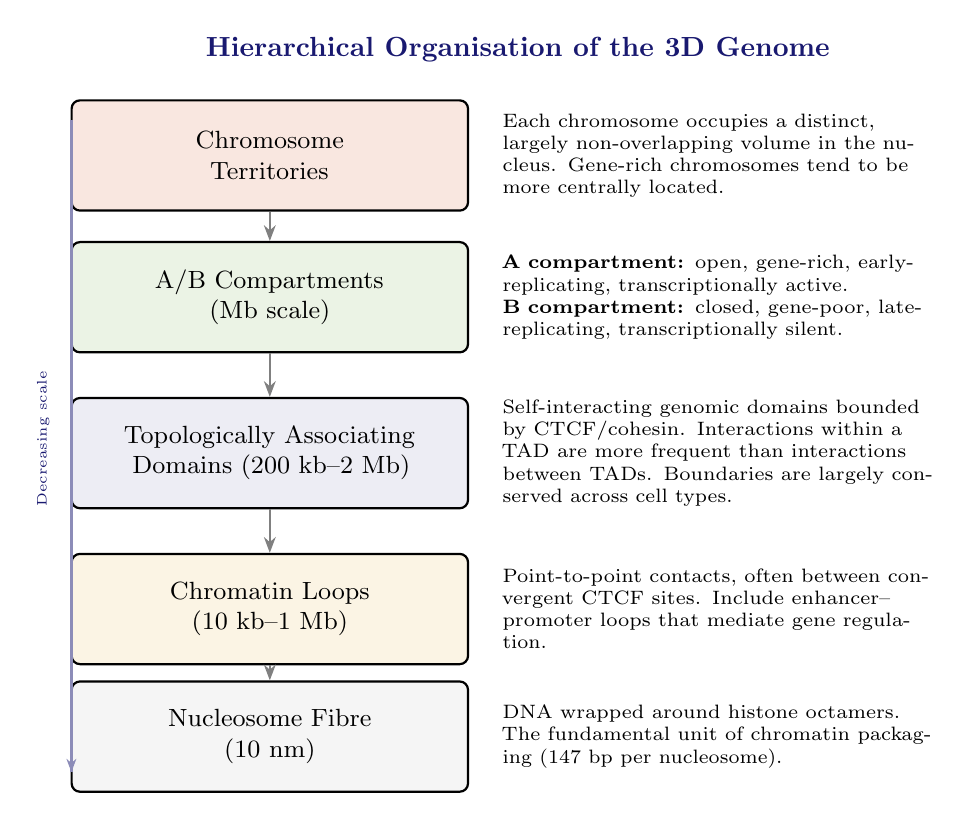
\begin{tikzpicture}[
  scale=0.9,
  level/.style={font=\small\bfseries, MidnightBlue},
  desc/.style={font=\scriptsize, text width=5.5cm},
  arrow/.style={-{Stealth[length=2mm]}, thick, gray},
  box/.style={draw, rounded corners=3pt, thick, minimum height=1.4cm, text width=4.8cm, align=center, font=\small}
]

% Title
\node[font=\bfseries, MidnightBlue] at (6, 10.5) {Hierarchical Organisation of the 3D Genome};

% Level 1: Chromosome territories
\node[box, fill=BrickRed!8] (ct) at (2.5, 9) {Chromosome\\Territories};
\node[desc, right=0.3cm of ct] {Each chromosome occupies a distinct, largely non-overlapping volume in the nucleus. Gene-rich chromosomes tend to be more centrally located.};

% Level 2: Compartments
\node[box, fill=OliveGreen!8] (comp) at (2.5, 7) {A/B Compartments\\(Mb scale)};
\node[desc, right=0.3cm of comp] {\textbf{A compartment:} open, gene-rich, early-replicating, transcriptionally active.\\
\textbf{B compartment:} closed, gene-poor, late-replicating, transcriptionally silent.};

% Level 3: TADs
\node[box, fill=MidnightBlue!8] (tad) at (2.5, 4.8) {Topologically Associating\\Domains (200 kb--2 Mb)};
\node[desc, right=0.3cm of tad] {Self-interacting genomic domains bounded by CTCF/cohesin. Interactions within a TAD are more frequent than interactions between TADs. Boundaries are largely conserved across cell types.};

% Level 4: Loops
\node[box, fill=Goldenrod!12] (loop) at (2.5, 2.6) {Chromatin Loops\\(10 kb--1 Mb)};
\node[desc, right=0.3cm of loop] {Point-to-point contacts, often between convergent CTCF sites. Include enhancer--promoter loops that mediate gene regulation.};

% Level 5: Nucleosomes
\node[box, fill=gray!8] (nuc) at (2.5, 0.8) {Nucleosome Fibre\\(10 nm)};
\node[desc, right=0.3cm of nuc] {DNA wrapped around histone octamers. The fundamental unit of chromatin packaging (147 bp per nucleosome).};

% Arrows
\draw[arrow] (ct.south) -- (comp.north);
\draw[arrow] (comp.south) -- (tad.north);
\draw[arrow] (tad.south) -- (loop.north);
\draw[arrow] (loop.south) -- (nuc.north);

% Scale bar
\draw[very thick, MidnightBlue!50] (-0.3, 9.5) -- (-0.3, 0.3);
\node[font=\tiny, MidnightBlue, rotate=90] at (-0.7, 5) {Decreasing scale};
\draw[-{Stealth}, MidnightBlue!50] (-0.3, 5) -- (-0.3, 0.3);

\end{tikzpicture}
\caption[Hierarchical levels of 3D genome organisation.]{The 3D genome is organised hierarchically, from chromosome territories (largest scale) to individual nucleosomes (smallest scale). Each level can be interrogated by specific sequencing-based methods: chromosome territories and A/B compartments by Hi-C eigenvector analysis, TADs by Hi-C and Micro-C at moderate resolution, and chromatin loops by high-resolution Hi-C, HiChIP, or Capture Hi-C.}
\label{fig:3dgenome:hierarchy}
\end{figure}

\subsection{Chromosome Territories}
\label{subsec:3dgenome:territories}

Each chromosome occupies a distinct, largely non-overlapping volume in the interphase nucleus called a \textbf{chromosome territory}. Gene-rich chromosomes (e.g., chr19) tend to reside in the nuclear interior, while gene-poor chromosomes (e.g., chr18) tend to be positioned near the nuclear periphery (lamina-associated). Chromosome territories can be visualised by fluorescence in situ hybridisation (FISH) with whole-chromosome paints.

\subsection{A/B Compartments}
\label{subsec:3dgenome:compartments}

At the megabase scale, the genome is partitioned into two types of compartments:

\begin{itemize}[itemsep=3pt]
  \item \textbf{A compartment:} euchromatic, gene-rich, transcriptionally active, early-replicating, enriched for active histone marks (H3K27ac, H3K4me3). Corresponds to open chromatin.
  \item \textbf{B compartment:} heterochromatic, gene-poor, transcriptionally silent, late-replicating, enriched for repressive marks (H3K27me3, H3K9me3) or lacking histone marks entirely. Corresponds to closed/compacted chromatin.
\end{itemize}

A/B compartments are identified from Hi-C data by performing principal component analysis (PCA) on the correlation matrix of Hi-C contact frequencies. The first eigenvector (PC1) separates the genome into A and B compartments. Compartment identity is dynamic and changes during differentiation, reprogramming, and disease.

\subsection{Topologically Associating Domains (TADs)}
\label{subsec:3dgenome:tads}

\textbf{TADs} are contiguous genomic regions (typically 200\kilobase{}--2\megabase{} in mammals) within which chromatin interactions are substantially more frequent than interactions crossing TAD boundaries. TADs appear as prominent ``triangles'' along the diagonal of Hi-C contact maps.

Key properties of TADs:
\begin{itemize}[itemsep=2pt]
  \item \textbf{Boundaries} are enriched for CTCF binding sites in convergent orientation, cohesin complex components, active promoters, and housekeeping genes.
  \item TAD boundaries are \textbf{largely conserved} across cell types and species, though sub-TAD organisation and loop contacts are more cell-type-specific.
  \item TADs serve as \textbf{regulatory domains}: enhancers within a TAD preferentially regulate genes within the same TAD.
  \item \textbf{Disruption of TAD boundaries} can cause enhancer hijacking---a mechanism implicated in developmental disorders (e.g., limb malformations) and cancer (e.g., oncogene activation).
\end{itemize}

\subsection{Chromatin Loops}
\label{subsec:3dgenome:loops}

Chromatin loops are specific point-to-point contacts between two genomic loci. The most prominent loops are mediated by \textbf{CTCF and cohesin}:

\begin{itemize}[itemsep=2pt]
  \item CTCF binds to its motif in a directional manner (the motif is asymmetric).
  \item Cohesin (a ring-shaped complex) extrudes chromatin until it encounters two convergently oriented CTCF sites (facing each other), forming a loop.
  \item This \textbf{loop extrusion model} explains how TADs and loops form: cohesin extrudes chromatin bidirectionally until blocked by convergent CTCF barriers.
\end{itemize}

\begin{keyconcept}[title={The Loop Extrusion Model}]
The loop extrusion model proposes that cohesin (or condensin) complexes are loaded onto chromatin and actively extrude DNA through their ring structure, progressively enlarging a chromatin loop. Extrusion halts when cohesin encounters CTCF proteins bound in convergent orientation, establishing a stable loop with CTCF at its anchors. This model elegantly explains: (1) why loops form preferentially between convergent CTCF sites; (2) why TADs are insulated domains; and (3) why cohesin depletion eliminates loops and TADs but not compartments. The model has been supported by polymer simulations, cohesin depletion experiments (using auxin-inducible degron systems), and live-cell imaging.
\end{keyconcept}

%% ============================================================
\section{Hi-C: Genome-Wide Chromosome Conformation Capture}
\label{sec:3dgenome:hic}

\subsection{Principle}
\label{subsec:3dgenome:hic-principle}

Hi-C is the most widely used method for mapping genome-wide chromatin interactions. It captures all pairwise contacts in the genome simultaneously:

\begin{enumerate}[itemsep=2pt]
  \item \textbf{Crosslinking:} Fix cells with formaldehyde to covalently link spatially proximal chromatin segments.
  \item \textbf{Restriction enzyme digestion:} Digest chromatin with a restriction enzyme (e.g., MboI, DpnII, or HindIII). The choice of enzyme determines the theoretical resolution limit.
  \item \textbf{Biotinylated fill-in:} Fill in the restriction enzyme overhangs with biotinylated nucleotides, marking the ligation junction.
  \item \textbf{Proximity ligation:} Under dilute conditions (or in situ within the nucleus), ligate the blunt ends. Fragments that were spatially proximal (regardless of their linear genomic distance) are preferentially ligated.
  \item \textbf{Biotin pull-down:} Shear the ligated DNA, pull down biotinylated junctions with streptavidin beads, and prepare a paired-end sequencing library.
  \item \textbf{Sequencing and mapping:} Each read pair represents a contact between two genomic loci. Map each end independently to the reference genome to identify the interacting pair.
\end{enumerate}

\begin{figure}[htbp]
\centering
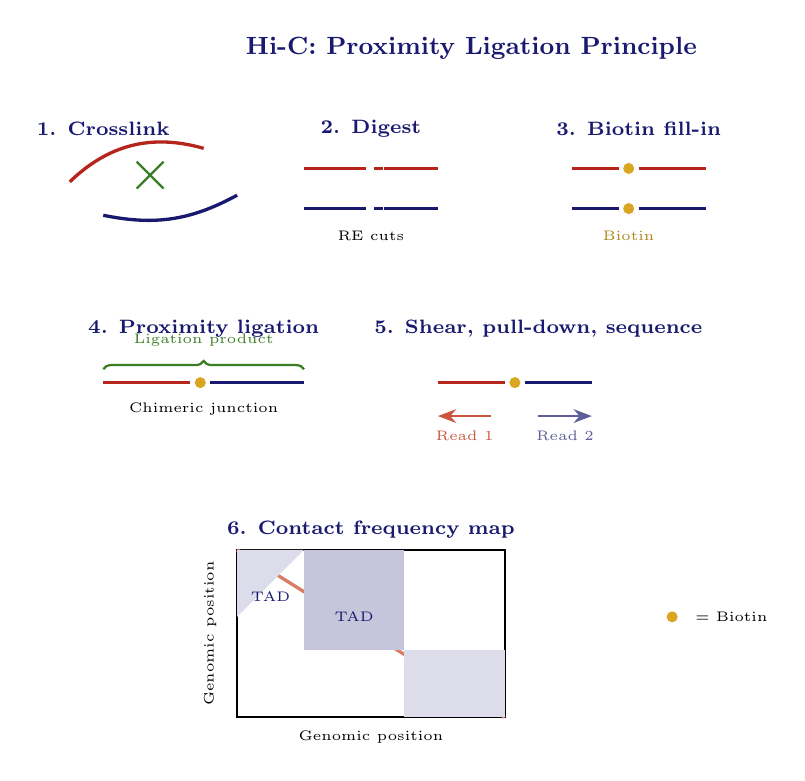
\begin{tikzpicture}[
  scale=0.85,
  box/.style={draw, rounded corners=3pt, thick, minimum width=3cm, minimum height=0.8cm, align=center, font=\scriptsize},
  arrow/.style={-{Stealth[length=2.5mm]}, thick, MidnightBlue},
  dna/.style={very thick},
  biotin/.style={circle, fill=Goldenrod, minimum size=4pt, inner sep=0pt}
]

% Title
\node[font=\bfseries\small, MidnightBlue] at (6, 10) {Hi-C: Proximity Ligation Principle};

% Step 1: Crosslinked chromatin
\node[font=\scriptsize\bfseries, MidnightBlue] at (0.5, 8.8) {1. Crosslink};
\draw[dna, BrickRed] (0, 8) to[bend left=30] (2, 8.5);
\draw[dna, MidnightBlue] (0.5, 7.5) to[bend right=20] (2.5, 7.8);
% Crosslink X
\node[font=\tiny, OliveGreen] at (1.2, 8.1) {$\times$};
\draw[OliveGreen, thick] (1, 8.3) -- (1.4, 7.9);
\draw[OliveGreen, thick] (1, 7.9) -- (1.4, 8.3);

% Step 2: Restriction digest
\node[font=\scriptsize\bfseries, MidnightBlue] at (4.5, 8.8) {2. Digest};
\draw[dna, BrickRed] (3.5, 8.2) -- (4.3, 8.2);
\draw[dna, BrickRed, dashed] (4.3, 8.2) -- (4.7, 8.2);
\draw[dna, BrickRed] (4.7, 8.2) -- (5.5, 8.2);
\draw[dna, MidnightBlue] (3.5, 7.6) -- (4.3, 7.6);
\draw[dna, MidnightBlue, dashed] (4.3, 7.6) -- (4.7, 7.6);
\draw[dna, MidnightBlue] (4.7, 7.6) -- (5.5, 7.6);
\node[font=\tiny] at (4.5, 7.2) {RE cuts};

% Step 3: Biotin fill-in
\node[font=\scriptsize\bfseries, MidnightBlue] at (8.5, 8.8) {3. Biotin fill-in};
\draw[dna, BrickRed] (7.5, 8.2) -- (8.2, 8.2);
\node[biotin] at (8.35, 8.2) {};
\draw[dna, BrickRed] (8.5, 8.2) -- (9.5, 8.2);
\draw[dna, MidnightBlue] (7.5, 7.6) -- (8.2, 7.6);
\node[biotin] at (8.35, 7.6) {};
\draw[dna, MidnightBlue] (8.5, 7.6) -- (9.5, 7.6);
\node[font=\tiny, Goldenrod!80!black] at (8.35, 7.2) {Biotin};

% Step 4: Proximity ligation
\node[font=\scriptsize\bfseries, MidnightBlue] at (2, 5.8) {4. Proximity ligation};
\draw[dna, BrickRed] (0.5, 5) -- (1.8, 5);
\node[biotin] at (1.95, 5) {};
\draw[dna, MidnightBlue] (2.1, 5) -- (3.5, 5);
\node[font=\tiny] at (2, 4.6) {Chimeric junction};
\draw[thick, OliveGreen, decorate, decoration={brace, amplitude=3pt}] (0.5, 5.2) -- (3.5, 5.2);
\node[font=\tiny, OliveGreen, above] at (2, 5.4) {Ligation product};

% Step 5: Purify and sequence
\node[font=\scriptsize\bfseries, MidnightBlue] at (7, 5.8) {5. Shear, pull-down, sequence};
\draw[dna, BrickRed] (5.5, 5) -- (6.5, 5);
\node[biotin] at (6.65, 5) {};
\draw[dna, MidnightBlue] (6.8, 5) -- (7.8, 5);
% Read arrows
\draw[{Stealth}-, thick, BrickRed!70] (5.5, 4.5) -- (6.3, 4.5);
\node[font=\tiny, BrickRed!70] at (5.9, 4.2) {Read 1};
\draw[-{Stealth}, thick, MidnightBlue!70] (7, 4.5) -- (7.8, 4.5);
\node[font=\tiny, MidnightBlue!70] at (7.4, 4.2) {Read 2};

% Step 6: Contact map
\node[font=\scriptsize\bfseries, MidnightBlue] at (4.5, 2.8) {6. Contact frequency map};
% Draw a small contact map
\draw[thick] (2.5, 0) rectangle (6.5, 2.5);
% Diagonal
\draw[very thick, BrickRed!50] (2.5, 2.5) -- (6.5, 0);
% TAD triangles
\fill[MidnightBlue!15] (2.5, 2.5) -- (3.5, 2.5) -- (2.5, 1.5) -- cycle;
\fill[MidnightBlue!25] (3.5, 2.5) -- (5, 2.5) -- (5, 1) -- (3.5, 1) -- cycle;
\fill[MidnightBlue!15] (5, 1) -- (6.5, 1) -- (6.5, 0) -- (5, 0) -- cycle;
% Labels
\node[font=\tiny] at (4.5, -0.3) {Genomic position};
\node[font=\tiny, rotate=90] at (2.1, 1.25) {Genomic position};
\node[font=\tiny, MidnightBlue] at (3.0, 1.8) {TAD};
\node[font=\tiny, MidnightBlue] at (4.25, 1.5) {TAD};

% Biotin legend
\node[biotin] at (9, 1.5) {};
\node[font=\tiny, right] at (9.2, 1.5) {= Biotin};

\end{tikzpicture}
\caption[Hi-C proximity ligation principle.]{The Hi-C method. (1) Cells are crosslinked with formaldehyde to preserve spatial proximity. (2) Chromatin is digested with a restriction enzyme. (3) Overhangs are filled in with biotinylated nucleotides. (4) Spatially proximal fragments are ligated, creating chimeric junctions. (5) DNA is sheared, biotinylated junctions are pulled down, and paired-end sequencing is performed. (6) Read pairs are mapped to the genome to generate a contact frequency matrix (heatmap), where TADs appear as prominent triangles along the diagonal.}
\label{fig:3dgenome:hic-principle}
\end{figure}

\subsection{In Situ Hi-C vs.\ Dilution Hi-C}
\label{subsec:3dgenome:insitu-dilution}

\begin{itemize}[itemsep=3pt]
  \item \textbf{Dilution Hi-C (original method):} After restriction digestion, chromatin is highly diluted before ligation to promote intra-molecular (proximity) ligation over random inter-molecular ligation. This reduces noise but requires large cell numbers and has lower efficiency.
  \item \textbf{In situ Hi-C:} Ligation is performed inside intact nuclei, which naturally constrains ligation to spatially proximal fragments without the need for dilution. This produces higher-quality contact maps with less noise and is now the standard approach.
\end{itemize}

\subsection{Resolution and Sequencing Depth}
\label{subsec:3dgenome:resolution}

The resolution of a Hi-C contact map depends on sequencing depth:

\begin{table}[htbp]
\centering
\caption{Hi-C resolution as a function of sequencing depth (human genome).}
\label{tab:3dgenome:resolution}
\small
\begin{tabular}{l c l}
\toprule
\textbf{Resolution} & \textbf{Read Pairs Required} & \textbf{Features Resolved} \\
\midrule
1\megabase{} & $\sim$10 million & A/B compartments \\
100\kilobase{} & $\sim$100 million & TADs \\
40\kilobase{} & $\sim$300--500 million & TADs, sub-TADs \\
10\kilobase{} & $\sim$1 billion & Chromatin loops \\
5\kilobase{} & $\sim$2--3 billion & Fine loop architecture \\
1\kilobase{} & $\sim$10+ billion & Micro-C level detail \\
\bottomrule
\end{tabular}
\end{table}

\begin{warningbox}
Hi-C is one of the most sequencing-intensive methods in genomics. Achieving 1\kilobase{} resolution across a human genome requires $>$10 billion read pairs, costing tens of thousands of dollars. Most published Hi-C datasets are at 5--40\kilobase{} resolution. When designing a Hi-C experiment, carefully consider the resolution needed for your biological question and budget accordingly.
\end{warningbox}

\subsection{Hi-C Library Preparation Kits}
\label{subsec:3dgenome:hic-kits}

\begin{itemize}[itemsep=2pt]
  \item \textbf{Arima Hi-C:} Uses a cocktail of multiple restriction enzymes for finer fragmentation, achieving higher resolution per sequencing read. Widely used for both chromatin conformation and genome scaffolding.
  \item \textbf{Dovetail Omni-C:} Uses a sequence-independent chromatin fragmentation approach (DNase-based rather than restriction enzymes), eliminating restriction enzyme bias and providing more uniform coverage. Can be used for both 3D genome mapping and genome assembly scaffolding.
  \item \textbf{Phase Genomics ProxiMeta:} Hi-C kits optimised for metagenome deconvolution and assembly.
\end{itemize}

%% ============================================================
\section{Micro-C}
\label{sec:3dgenome:microc}

\textbf{Micro-C} replaces the restriction enzyme in Hi-C with micrococcal nuclease (MNase), which digests linker DNA between nucleosomes. This achieves \textbf{nucleosome-level resolution} ($\sim$200\basepair{}):

\begin{itemize}[itemsep=2pt]
  \item Improved resolution at short-range interactions ($<$ 10\kilobase{}).
  \item Reveals fine-scale chromatin folding features (``stripes,'' ``dots'') not visible in standard Hi-C.
  \item Better signal-to-noise ratio for loop detection at moderate sequencing depths.
  \item Requires similar sequencing depths to Hi-C for genome-wide maps but provides superior resolution per read.
\end{itemize}

\begin{tipbox}
For new chromatin conformation experiments where fine-scale loop detection is important, Micro-C offers advantages over restriction enzyme-based Hi-C. However, Hi-C remains the more established method with the larger existing dataset ecosystem and better standardised analysis pipelines.
\end{tipbox}

%% ============================================================
\section{Targeted and Enrichment-Based 3C Methods}
\label{sec:3dgenome:targeted}

\subsection{Capture Hi-C / Promoter Capture Hi-C}
\label{subsec:3dgenome:capture-hic}

Standard Hi-C distributes sequencing reads across all pairwise contacts genome-wide, making it expensive to achieve high resolution at specific loci. \textbf{Capture Hi-C} enriches Hi-C libraries for contacts involving specific regions of interest using hybridisation capture:

\begin{itemize}[itemsep=2pt]
  \item \textbf{Promoter Capture Hi-C (PCHi-C):} Uses capture probes targeting all annotated gene promoters. Identifies enhancer--promoter interactions at specific genes without the cost of deep genome-wide Hi-C.
  \item \textbf{Region Capture Hi-C:} Capture probes target specific genomic regions (e.g., disease-associated loci) to map their interaction partners.
  \item Achieves high resolution ($\sim$1--4 restriction fragment resolution) at target loci with modest sequencing (100--200M read pairs).
\end{itemize}

\subsection{HiChIP and PLAC-seq}
\label{subsec:3dgenome:hichip}

HiChIP and PLAC-seq combine chromatin conformation capture with ChIP to map \textbf{contacts at specific protein binding sites or histone modifications}:

\begin{itemize}[itemsep=3pt]
  \item \textbf{H3K27ac HiChIP:} The most widely used variant. Maps contacts between active regulatory elements (enhancers and promoters marked by H3K27ac), directly identifying active enhancer--promoter loops.
  \item \textbf{Cohesin HiChIP (SMC1A/RAD21):} Maps contacts at cohesin-mediated loops, identifying architectural loop anchors.
  \item \textbf{CTCF HiChIP:} Maps contacts at CTCF binding sites, revealing insulator-mediated loops and TAD boundaries.
  \item Requires far fewer reads than genome-wide Hi-C (50--200M per sample) because the antibody enrichment focuses sequencing depth on informative contacts.
\end{itemize}

\subsection{ChIA-PET}
\label{subsec:3dgenome:chiapet}

Chromatin Interaction Analysis by Paired-End Tag sequencing (ChIA-PET) is an earlier method similar to HiChIP that uses ChIP followed by proximity ligation and paired-end tag sequencing. ChIA-PET was pioneered for CTCF and RNA Pol II and has been largely superseded by HiChIP due to the latter's simpler protocol and higher efficiency.

%% ============================================================
\section{Long-Read and Alternative 3D Genome Methods}
\label{sec:3dgenome:alternative}

\subsection{Pore-C (Oxford Nanopore)}
\label{subsec:3dgenome:porec}

Pore-C combines proximity ligation with nanopore long-read sequencing to capture \textbf{multi-way chromatin contacts}:

\begin{itemize}[itemsep=2pt]
  \item Standard Hi-C reads contain only one ligation junction per read pair (pairwise contact). Pore-C long reads ($>$10\kilobase{}) can span \textbf{multiple ligation junctions}, revealing multi-way contacts (three or more fragments ligated together).
  \item Multi-way contacts provide information about \textbf{chromatin hubs}---regions where multiple genomic loci converge in 3D space simultaneously.
  \item Also useful for \textbf{genome scaffolding} in de novo assembly.
\end{itemize}

\subsection{SPRITE}
\label{subsec:3dgenome:sprite}

Split-Pool Recognition of Interactions by Tag Extension (SPRITE) captures multi-way chromatin contacts without proximity ligation:

\begin{enumerate}[itemsep=2pt]
  \item Crosslink cells and fragment chromatin.
  \item Split crosslinked chromatin complexes into 96-well plates and add a unique barcode (tag) in each well.
  \item Pool and re-split into new plates for additional rounds of barcoding.
  \item After multiple rounds, each chromatin complex carries a unique combination of barcodes (a ``barcode string'') that identifies all fragments in the same complex.
  \item Sequence and group fragments by shared barcode strings to identify multi-way contacts.
\end{enumerate}

SPRITE can detect \textbf{higher-order interactions} (contacts among many loci simultaneously) and has revealed hub-like structures associated with nuclear bodies (nucleolus, nuclear speckles).

\subsection{GAM (Genome Architecture Mapping)}
\label{subsec:3dgenome:gam}

GAM slices nuclei into thin cryosections, extracts DNA from each section, and sequences it. Loci that are spatially proximal are more likely to appear in the same nuclear section. By sequencing many sections, a contact frequency map is reconstructed. GAM does not require proximity ligation and can also detect multi-way contacts. It has been particularly useful for mapping \textbf{lamina-associated domains (LADs)}---regions of the genome that interact with the nuclear lamina and are typically transcriptionally silent.

\subsection{DNA-FISH and Live Imaging}
\label{subsec:3dgenome:imaging}

While not sequencing-based, imaging methods provide important complementary information:

\begin{itemize}[itemsep=2pt]
  \item \textbf{DNA-FISH:} Fluorescence in situ hybridisation with locus-specific probes allows direct measurement of spatial distances between genomic loci in individual cells. Validates Hi-C-predicted contacts.
  \item \textbf{Multiplexed FISH (ORCA, chromatin tracing):} Sequential rounds of hybridisation and imaging map the 3D positions of hundreds to thousands of genomic loci in single cells, providing single-cell 3D genome structure data.
  \item \textbf{Live-cell imaging:} CRISPR-Cas9-based labelling or MS2/PP7 RNA tagging enables real-time tracking of locus dynamics in living cells.
\end{itemize}

%% ============================================================
\section{Comprehensive Comparison of 3D Genome Methods}
\label{sec:3dgenome:comparison}

\begin{table}[htbp]
\centering
\caption[Comparison of 3D genome profiling methods.]{Comparison of major methods for mapping three-dimensional genome organisation.}
\label{tab:3dgenome:comparison}
\small
\begin{tabularx}{\textwidth}{l c c c X}
\toprule
\textbf{Method} & \textbf{Resolution} & \textbf{Read Pairs} & \textbf{Multi-way?} & \textbf{Key Features} \\
\midrule
Hi-C & 1 kb--1 Mb & 100M--3B & No (pairwise) & Gold standard; genome-wide all-vs-all \\
\addlinespace
Micro-C & $\sim$200 bp & 100M--3B & No & Nucleosome resolution; superior short-range \\
\addlinespace
Capture Hi-C & 1--4 RE fragments & 100--200M & No & Targeted enrichment; cost-effective for loci \\
\addlinespace
HiChIP & 5--10 kb & 50--200M & No & ChIP + proximity ligation; active loops \\
\addlinespace
ChIA-PET & 5--10 kb & 50--200M & No & Earlier version of HiChIP; largely replaced \\
\addlinespace
Pore-C & $\sim$1 kb & 50--200M reads & Yes & Long-read; multi-way contacts \\
\addlinespace
SPRITE & $\sim$1 Mb & Variable & Yes & Ligation-free; nuclear body hubs \\
\addlinespace
GAM & $\sim$30 kb & Variable & Yes & Cryosectioning; no ligation; LADs \\
\bottomrule
\end{tabularx}
\end{table}

%% ============================================================
\section{Bioinformatics Workflow for Hi-C}
\label{sec:3dgenome:bioinformatics}

\subsection{Analysis Overview}
\label{subsec:3dgenome:analysis-overview}

Hi-C data analysis follows a distinct pipeline from other sequencing assays because each read pair represents a chromatin contact rather than a contiguous genomic fragment:

\begin{enumerate}[itemsep=2pt]
  \item \textbf{Read alignment:} Each mate of a read pair is aligned independently to the reference genome (because the two ends may originate from different chromosomes or distant loci). Aligners: BWA-MEM (with chimeric read handling), chromap, or the aligner built into specific pipelines.
  \item \textbf{Contact pair identification:} Valid Hi-C contacts (``pairs'') are identified from read pairs that map to different restriction fragments. Invalid pairs (self-ligations, dangling ends, PCR duplicates) are filtered.
  \item \textbf{Contact matrix generation:} Valid pairs are binned into a contact frequency matrix at a chosen resolution (bin size). Common formats: \texttt{.cool} (cooler), \texttt{.hic} (Juicer), or \texttt{.mcool} (multi-resolution cooler).
  \item \textbf{Normalisation:} The raw contact matrix contains biases from GC content, mappability, restriction site density, and other factors. Normalisation methods include:
    \begin{itemize}[itemsep=1pt]
      \item \textbf{ICE (Iterative Correction and Eigenvector decomposition):} Matrix balancing that equalises the total signal per row/column. The most widely used method. Implemented in cooler.
      \item \textbf{KR (Knight-Ruiz):} A faster matrix balancing algorithm. Default in Juicer.
      \item \textbf{VC (Vanilla Coverage):} Simple normalisation by the product of row and column sums.
    \end{itemize}
  \item \textbf{Feature calling:}
    \begin{itemize}[itemsep=1pt]
      \item \textbf{Compartments:} PCA on the contact correlation matrix (cooltools or HOMER).
      \item \textbf{TADs:} TopDom, Arrowhead (Juicer), HiCExplorer \texttt{hicFindTADs}, or insulation score methods.
      \item \textbf{Loops:} HICCUPS (Juicer), Mustache, Chromosight, or cooltools \texttt{dots}.
    \end{itemize}
  \item \textbf{Visualisation:} HiGlass (web-based interactive viewer), Juicebox (desktop application), HiCExplorer \texttt{hicPlotMatrix}, or cooltools for programmatic access.
  \item \textbf{Integration:} Overlay Hi-C contacts with epigenomic tracks (ATAC-seq, ChIP-seq, RNA-seq) to link 3D structure to function.
\end{enumerate}

The following subsections describe the key computational methods for normalisation, TAD calling, compartment identification, and polymer physics models in greater detail.

\subsection{Contact Matrix Normalisation Methods}
\label{subsec:3dgenome:normalisation}

Raw Hi-C contact matrices contain systematic biases arising from variable restriction site density, GC content, mappability, and chromatin accessibility across the genome. Normalisation removes these biases to produce matrices that more faithfully represent true contact frequencies. Three major normalisation approaches are in common use.

\subsubsection{ICE (Iterative Correction and Eigenvector Decomposition)}
\label{subsubsec:3dgenome:ice}

ICE, implemented in the \software{cooler} ecosystem, is the most widely used normalisation method. It is based on the assumption that, in the absence of systematic biases, each genomic locus should participate in approximately the same total number of contacts. The algorithm proceeds iteratively:

\begin{enumerate}[itemsep=2pt]
  \item Let $\mathbf{M}$ be the raw $N \times N$ contact matrix, where $M_{ij}$ is the number of contacts between bins $i$ and $j$.
  \item At each iteration, compute the total contacts (row/column sum) for each bin: $S_i = \sum_j M_{ij}$.
  \item Divide each row and column by the square root of its sum to produce a partially corrected matrix:
\end{enumerate}
\begin{equation}
\label{eq:3dgenome:ice-step}
M_{ij}^{(t+1)} = \frac{M_{ij}^{(t)}}{\sqrt{S_i^{(t)} \cdot S_j^{(t)}}}
\end{equation}
\begin{enumerate}[resume, itemsep=2pt]
  \item Repeat until convergence, defined as the point where all row and column sums are approximately equal.
  \item The final normalised matrix $\tilde{\mathbf{M}}$ has balanced margins (equal row/column sums), and the bias vector $\mathbf{b}$ (product of all per-iteration normalisation factors) captures the per-bin biases.
\end{enumerate}

Bins with very low contact counts (e.g., unmappable or repetitive regions) are excluded from balancing by applying a \textbf{mad-max filter}: bins whose log-transformed total counts deviate by more than a threshold (default: 5 median absolute deviations) from the median are masked.

\subsubsection{KR (Knight--Ruiz) Balancing}
\label{subsubsec:3dgenome:kr}

The Knight--Ruiz (KR) algorithm achieves the same goal as ICE---equalising row and column sums---but uses a faster, mathematically rigorous matrix balancing procedure. KR finds diagonal matrices $\mathbf{D}_1$ and $\mathbf{D}_2$ such that the normalised matrix $\tilde{\mathbf{M}} = \mathbf{D}_1 \mathbf{M} \mathbf{D}_2$ has equal row sums and equal column sums. For symmetric matrices (as in Hi-C), $\mathbf{D}_1 = \mathbf{D}_2 = \mathbf{D}$, and the balanced matrix is:
\begin{equation}
\label{eq:3dgenome:kr}
\tilde{M}_{ij} = \frac{M_{ij}}{d_i \cdot d_j}
\end{equation}
where $d_i$ are the diagonal elements of $\mathbf{D}$, found by an iterative algorithm that converges faster than ICE. KR normalisation is the default in \software{Juicer} and produces results very similar to ICE.

\subsubsection{VC (Vanilla Coverage) Normalisation}
\label{subsubsec:3dgenome:vc}

VC normalisation is the simplest approach: each contact count is divided by the product of the marginal sums of its row and column:
\begin{equation}
\label{eq:3dgenome:vc}
\tilde{M}_{ij} = \frac{M_{ij}}{S_i \cdot S_j} \times C
\end{equation}
where $S_i = \sum_j M_{ij}$, $S_j = \sum_i M_{ij}$, and $C$ is a constant (e.g., the total number of contacts) to keep values in a reasonable range. VC is a single-step procedure (no iteration) and is fast, but it over-corrects for highly interacting loci and is less robust than ICE or KR. It is mainly used as a baseline or for quick exploratory analyses.

\begin{tipbox}
For most analyses, ICE (cooler) or KR (Juicer) normalisation is recommended. The two methods produce highly concordant results ($r > 0.99$ for most genomic regions). The choice is often driven by the analysis ecosystem: use ICE with the cooler/cooltools pipeline, and KR with the Juicer pipeline. Always exclude low-coverage bins from normalisation to prevent artefacts from unmappable regions.
\end{tipbox}

\subsection{TAD Calling Algorithms}
\label{subsec:3dgenome:tad-calling}

Topologically associating domains (TADs) are self-interacting chromosomal regions where loci interact more frequently with each other than with loci in neighbouring domains. TAD boundaries are enriched for CTCF binding sites and often demarcate regulatory neighbourhoods. Two principal algorithms for TAD identification are the insulation score and the directionality index.

\subsubsection{Insulation Score}
\label{subsubsec:3dgenome:insulation}

The insulation score, originally proposed by Crane et al., quantifies the degree of insulation at each genomic bin by examining the average interaction frequency in a square diamond window centred on the bin's position along the matrix diagonal:

\begin{enumerate}[itemsep=2pt]
  \item For each bin $i$, define a diamond-shaped window spanning $w$ bins upstream and $w$ bins downstream of $i$. This window captures contacts \textit{across} position $i$---i.e., interactions between the region upstream of $i$ and the region downstream.
  \item Compute the insulation score as the mean contact frequency within this diamond:
\end{enumerate}
\begin{equation}
\label{eq:3dgenome:insulation-score}
\text{IS}(i) = \log_2\!\left(\frac{1}{w^2}\sum_{i-w \leq a < i}\;\sum_{i < b \leq i+w} M_{a,b}\right)
\end{equation}
\begin{enumerate}[resume, itemsep=2pt]
  \item Normalise the insulation scores to the genome-wide mean.
  \item TAD boundaries correspond to \textbf{local minima} in the insulation score profile---positions where cross-boundary interactions are depleted relative to within-domain interactions.
  \item The depth of the minimum (``boundary strength'') quantifies how strong the insulation is at each boundary.
\end{enumerate}

The window size $w$ (in bins) is a critical parameter. Smaller windows ($\sim$100--250\kilobase{}) detect smaller TADs; larger windows ($\sim$500\kilobase{}--1\megabase{}) detect larger domains. The insulation score method is implemented in \software{cooltools insulation}.

\subsubsection{Directionality Index}
\label{subsubsec:3dgenome:di}

The directionality index (DI), introduced by Dixon et al., captures the asymmetry between upstream and downstream interactions at each bin. Within a TAD, bins near the upstream boundary interact preferentially downstream (toward the domain interior), while bins near the downstream boundary interact preferentially upstream:

\begin{equation}
\label{eq:3dgenome:di}
\text{DI}(i) = \left(\frac{B_i - A_i}{|B_i - A_i|}\right) \cdot \frac{(A_i - E)^2 + (B_i - E)^2}{E}
\end{equation}
where $A_i = \sum_{j=i-w}^{i-1} M_{ij}$ is the total upstream contact frequency, $B_i = \sum_{j=i+1}^{i+w} M_{ij}$ is the total downstream contact frequency, and $E = (A_i + B_i)/2$ is the expected value under the null hypothesis of no directional bias.

\begin{itemize}[itemsep=2pt]
  \item \textbf{DI $> 0$} (downstream bias): the bin interacts more with downstream neighbours, indicating the upstream portion of a TAD.
  \item \textbf{DI $< 0$} (upstream bias): the bin interacts more with upstream neighbours, indicating the downstream portion of a TAD.
  \item \textbf{DI $\approx 0$}: no directional preference (interior of a TAD or inter-TAD region).
  \item A \textbf{hidden Markov model} is then applied to the DI profile to segment the genome into domains. Transitions from negative to positive DI correspond to TAD boundaries.
\end{itemize}

The DI approach is implemented in the original \software{Juicer/Arrowhead} tool and in \software{HiCExplorer hicFindTADs}.

\subsection{Compartment Analysis}
\label{subsec:3dgenome:compartments}

At the megabase scale, the genome is partitioned into two types of compartments: \textbf{A compartments} (active, gene-rich, open chromatin) and \textbf{B compartments} (inactive, gene-poor, closed chromatin). These compartments manifest as a ``checkerboard'' (plaid) pattern in the Hi-C contact matrix.

\subsubsection{Eigenvector Decomposition}
\label{subsubsec:3dgenome:eigenvector}

Compartments are identified by \textbf{principal component analysis (PCA)} of the observed/expected (O/E) contact correlation matrix:

\begin{enumerate}[itemsep=2pt]
  \item Compute the expected contact frequency $E_{ij}$ for each pair of bins as a function of genomic distance (the average contact frequency at that distance).
  \item Construct the O/E matrix: $\text{OE}_{ij} = M_{ij} / E_{ij}$.
  \item Compute the \textbf{Pearson correlation matrix} of the O/E matrix: each row $i$ of the O/E matrix defines a contact profile for bin $i$, and the correlation matrix captures the similarity of contact profiles between pairs of bins.
  \item Perform eigendecomposition of the correlation matrix. The \textbf{first eigenvector (PC1)} captures the strongest pattern of co-variation in contact profiles, which corresponds to the A/B compartment structure.
  \item Bins with \textbf{positive PC1 values} belong to one compartment, and bins with \textbf{negative PC1 values} belong to the other.
\end{enumerate}

\textbf{A/B assignment.} The sign of the eigenvector is arbitrary (PCA does not assign biological labels). To resolve this ambiguity, the eigenvector is correlated with GC content or gene density: the compartment with higher GC content and gene density is labelled \textbf{A} (active), and the other is labelled \textbf{B} (inactive). In most cell types:
\begin{itemize}[itemsep=2pt]
  \item \textbf{A compartments:} euchromatic, high gene density, high GC content, enriched for H3K27ac and H3K4me1, actively transcribed.
  \item \textbf{B compartments:} heterochromatic, low gene density, low GC content, enriched for H3K9me3 or H3K27me3, often lamina-associated.
\end{itemize}

Compartment analysis is performed at coarse resolution (50--250\kilobase{} bins) and is implemented in \software{cooltools eigs-cis} and \software{Juicer eigenvector}.

\subsection{Polymer Physics Models of Chromatin Folding}
\label{subsec:3dgenome:polymer-physics}

The three-dimensional folding of chromatin can be described using concepts from \textbf{polymer physics}. These models provide a theoretical framework for interpreting the distance-dependent decay of contact frequencies observed in Hi-C data.

\subsubsection{Contact Probability Scaling}

A fundamental observation from Hi-C data is that the probability of two loci being in contact decreases as a power law with increasing genomic distance:
\begin{equation}
\label{eq:3dgenome:contact-scaling}
P(s) \propto s^{-\gamma}
\end{equation}
where $P(s)$ is the contact probability at genomic separation $s$ (in base pairs) and $\gamma$ is the scaling exponent. The value of $\gamma$ reveals information about the polymer organisation of chromatin:

\begin{itemize}[itemsep=3pt]
  \item \textbf{Equilibrium globule} (random polymer in confinement): $\gamma \approx 1.5$. In this model, the polymer has reached thermodynamic equilibrium, and distant loci have very low contact probability. Early Hi-C experiments showed that chromatin does \textit{not} behave as an equilibrium globule.
  \item \textbf{Fractal globule}: $\gamma \approx 1.0$. The fractal globule is a \textbf{knot-free} polymer conformation that has not reached equilibrium. It is characterised by self-similar organisation at multiple scales and the absence of topological entanglements. The original Lieberman-Aiden et al.\ (2009) Hi-C study found $\gamma \approx 1.08$ for human chromatin, closely matching fractal globule predictions.
  \item \textbf{Loop extrusion model}: $\gamma$ varies with scale. At short ranges ($<$ 100\kilobase{}), $\gamma$ is influenced by loop extrusion dynamics; at intermediate ranges (100\kilobase{}--10\megabase{}), $\gamma \approx 0.75$--$1.0$; at very long ranges ($>$ 10\megabase{}), $\gamma$ reflects compartmentalisation.
\end{itemize}

\subsubsection{Loop Extrusion Model}

The \textbf{loop extrusion model} is the current leading framework for explaining TAD formation and loop establishment:

\begin{enumerate}[itemsep=2pt]
  \item A \textbf{cohesin ring complex} (SMC1/SMC3/RAD21/SA1--2) loads onto chromatin and begins \textbf{actively extruding a loop} by translocating along the chromatin fibre in both directions.
  \item As cohesin moves, the chromatin on either side of the loading site is progressively reeled through the ring, forming an expanding loop.
  \item When a cohesin subunit encounters a \textbf{CTCF protein bound in convergent orientation} (the CTCF motifs at the two anchors point toward each other: $\rightarrow \cdots \leftarrow$), loop extrusion is \textbf{blocked}. This stalling creates a stable loop with CTCF-bound anchors.
  \item Loops formed by convergent CTCF sites correspond to the bright ``dots'' seen at the corners of TADs in Hi-C contact maps.
  \item The loop extrusion process dynamically maintains TAD structures and is essential for proper enhancer--promoter regulation by confining regulatory contacts within domains.
\end{enumerate}

\begin{keyconcept}[title={The Loop Extrusion Paradigm}]
Loop extrusion by cohesin, blocked by convergent CTCF sites, explains three key features of 3D genome organisation simultaneously: (1) TAD boundaries coincide with convergent CTCF sites, (2) TAD structure is lost upon cohesin degradation (but restored upon cohesin recovery), and (3) CTCF site deletions or orientation inversions alter loop structure in predictable ways. This model has been validated by acute protein degradation experiments (auxin-inducible degron systems for RAD21 and CTCF), polymer simulations, and CRISPR-mediated CTCF site editing.
\end{keyconcept}

\subsection{Snakemake Workflow}
\label{subsec:3dgenome:snakemake}

\begin{lstlisting}[language=Python, caption={Snakemake workflow for Hi-C analysis.}, label={lst:3dgenome:snakemake}]
# Snakefile for Hi-C analysis
configfile: "config.yaml"

SAMPLES = config["samples"]
GENOME = config["genome_fasta"]
GENOME_INDEX = config["genome_bwa_index"]
CHROMSIZES = config["chromsizes"]
RESOLUTION = config["resolution"]  # e.g., 10000

rule all:
    input:
        expand("results/cool/{sample}.mcool", sample=SAMPLES),
        expand("results/compartments/{sample}_compartments.bed",
               sample=SAMPLES),
        expand("results/tads/{sample}_tads.bed",
               sample=SAMPLES),
        expand("results/loops/{sample}_loops.bedpe",
               sample=SAMPLES),
        expand("results/plots/{sample}_contact_map.png",
               sample=SAMPLES),
        "results/multiqc/multiqc_report.html"

rule align_hic:
    input:
        r1 = "raw_data/{sample}_R1.fastq.gz",
        r2 = "raw_data/{sample}_R2.fastq.gz"
    output:
        pairs = "results/pairs/{sample}.pairs.gz",
        stats = "results/pairs/{sample}.stats"
    threads: 16
    resources:
        mem_mb = 64000
    conda: "envs/hic.yaml"
    shell:
        """
        # Align with BWA-MEM, parse to pairs format
        # using pairtools for chimeric read handling
        bwa mem -t {threads} -SP5M {GENOME_INDEX} \
            {input.r1} {input.r2} \
        | pairtools parse --min-mapq 30 \
            --chroms-path {CHROMSIZES} \
            --walks-policy 5unique \
            --output-stats {output.stats} \
        | pairtools sort --nproc {threads} \
        | pairtools dedup \
            --max-mismatch 3 \
            --mark-dups \
            --output - \
        | pairtools select '(chrom1 != "chrM") and \
            (chrom2 != "chrM")' \
        | pairtools split \
            --output-pairs {output.pairs}
        """

rule create_cool:
    input:
        pairs = "results/pairs/{sample}.pairs.gz"
    output:
        cool = "results/cool/{sample}.cool"
    params:
        resolution = RESOLUTION
    conda: "envs/hic.yaml"
    shell:
        """
        cooler cload pairs \
            -c1 2 -p1 3 -c2 4 -p2 5 \
            --assembly hg38 \
            {CHROMSIZES}:{params.resolution} \
            {input.pairs} {output.cool}
        """

rule balance_and_zoomify:
    input:
        cool = "results/cool/{sample}.cool"
    output:
        mcool = "results/cool/{sample}.mcool"
    conda: "envs/hic.yaml"
    shell:
        """
        cooler balance {input.cool} --force
        cooler zoomify {input.cool} \
            --resolutions 1000,5000,10000,25000,50000,\
100000,250000,500000,1000000 \
            --balance \
            --out {output.mcool}
        """

rule call_compartments:
    input:
        mcool = "results/cool/{sample}.mcool"
    output:
        compartments = "results/compartments/{sample}_compartments.bed",
        eigenvector = "results/compartments/{sample}_eigenvector.bw"
    params:
        resolution = 100000
    conda: "envs/hic.yaml"
    shell:
        """
        cooltools eigs-cis \
            {input.mcool}::resolutions/{params.resolution} \
            --n-eigs 3 \
            -o results/compartments/{wildcards.sample}

        # Convert eigenvector to BED for A/B assignment
        python scripts/eigenvector_to_compartments.py \
            results/compartments/{wildcards.sample}.cis.vecs.tsv \
            {output.compartments}
        """

rule call_tads:
    input:
        mcool = "results/cool/{sample}.mcool"
    output:
        tads = "results/tads/{sample}_tads.bed",
        insulation = "results/tads/{sample}_insulation.bw"
    params:
        resolution = 25000,
        window = 500000
    conda: "envs/hic.yaml"
    shell:
        """
        cooltools insulation \
            {input.mcool}::resolutions/{params.resolution} \
            --window-pixels {params.window} \
            -o results/tads/{wildcards.sample}_insulation.tsv

        python scripts/insulation_to_tads.py \
            results/tads/{wildcards.sample}_insulation.tsv \
            {output.tads}
        """

rule call_loops:
    input:
        mcool = "results/cool/{sample}.mcool"
    output:
        loops = "results/loops/{sample}_loops.bedpe"
    params:
        resolution = 10000
    conda: "envs/hic.yaml"
    shell:
        """
        mustache -f {input.mcool} \
            -r {params.resolution} \
            -o {output.loops} \
            -pt 0.05 -st 0.88
        """

rule plot_contact_map:
    input:
        mcool = "results/cool/{sample}.mcool"
    output:
        plot = "results/plots/{sample}_contact_map.png"
    params:
        resolution = 25000,
        region = config.get("plot_region", "chr1:50000000-55000000")
    conda: "envs/hic.yaml"
    shell:
        """
        hicPlotMatrix --matrix {input.mcool} \
            --region {params.region} \
            --log1p \
            --colorMap RdYlBu_r \
            --outFileName {output.plot} \
            --dpi 300
        """

rule multiqc:
    input:
        expand("results/pairs/{sample}.stats", sample=SAMPLES)
    output:
        "results/multiqc/multiqc_report.html"
    conda: "envs/multiqc.yaml"
    shell:
        """
        multiqc results/ -o results/multiqc --force
        """
\end{lstlisting}

\subsection{Nextflow Workflow}
\label{subsec:3dgenome:nextflow}

\begin{lstlisting}[language=Java, caption={Nextflow DSL2 workflow for Hi-C analysis.}, label={lst:3dgenome:nextflow}]
#!/usr/bin/env nextflow
nextflow.enable.dsl=2

params.reads       = "raw_data/*_R{1,2}.fastq.gz"
params.genome      = "reference/genome.fa"
params.bwa_index   = "reference/genome"
params.chromsizes  = "reference/chromsizes.txt"
params.resolution  = 10000
params.outdir      = "results"
params.plot_region = "chr1:50000000-55000000"

process ALIGN_AND_PARSE {
    tag "$sample_id"
    cpus 16
    memory '64 GB'
    publishDir "${params.outdir}/pairs", mode: 'copy'

    input:
    tuple val(sample_id), path(reads)

    output:
    tuple val(sample_id),
          path("${sample_id}.pairs.gz"),   emit: pairs
    path "${sample_id}.stats",             emit: stats

    script:
    """
    bwa mem -t ${task.cpus} -SP5M \
        ${params.bwa_index} \
        ${reads[0]} ${reads[1]} \
    | pairtools parse --min-mapq 30 \
        --chroms-path ${params.chromsizes} \
        --walks-policy 5unique \
        --output-stats ${sample_id}.stats \
    | pairtools sort --nproc ${task.cpus} \
    | pairtools dedup --max-mismatch 3 \
        --mark-dups --output - \
    | pairtools select \
        '(chrom1 != "chrM") and (chrom2 != "chrM")' \
    | pairtools split \
        --output-pairs ${sample_id}.pairs.gz
    """
}

process CREATE_COOLER {
    tag "$sample_id"
    publishDir "${params.outdir}/cool", mode: 'copy'

    input:
    tuple val(sample_id), path(pairs)

    output:
    tuple val(sample_id),
          path("${sample_id}.mcool"),      emit: mcool

    script:
    """
    cooler cload pairs \
        -c1 2 -p1 3 -c2 4 -p2 5 \
        --assembly hg38 \
        ${params.chromsizes}:${params.resolution} \
        ${pairs} ${sample_id}.cool

    cooler balance ${sample_id}.cool --force

    cooler zoomify ${sample_id}.cool \
        --resolutions 1000,5000,10000,25000,50000,\
100000,250000,500000,1000000 \
        --balance \
        --out ${sample_id}.mcool
    """
}

process CALL_COMPARTMENTS {
    tag "$sample_id"
    publishDir "${params.outdir}/compartments",
               mode: 'copy'

    input:
    tuple val(sample_id), path(mcool)

    output:
    tuple val(sample_id),
          path("${sample_id}_compartments.bed"),
                                           emit: compartments
    path "${sample_id}*",                  emit: all_files

    script:
    """
    cooltools eigs-cis \
        ${mcool}::resolutions/100000 \
        --n-eigs 3 \
        -o ${sample_id}

    python ${projectDir}/scripts/eigenvector_to_compartments.py \
        ${sample_id}.cis.vecs.tsv \
        ${sample_id}_compartments.bed
    """
}

process CALL_TADS {
    tag "$sample_id"
    publishDir "${params.outdir}/tads", mode: 'copy'

    input:
    tuple val(sample_id), path(mcool)

    output:
    tuple val(sample_id),
          path("${sample_id}_tads.bed"),   emit: tads

    script:
    """
    cooltools insulation \
        ${mcool}::resolutions/25000 \
        --window-pixels 500000 \
        -o ${sample_id}_insulation.tsv

    python ${projectDir}/scripts/insulation_to_tads.py \
        ${sample_id}_insulation.tsv \
        ${sample_id}_tads.bed
    """
}

process CALL_LOOPS {
    tag "$sample_id"
    publishDir "${params.outdir}/loops", mode: 'copy'

    input:
    tuple val(sample_id), path(mcool)

    output:
    tuple val(sample_id),
          path("${sample_id}_loops.bedpe"),
                                           emit: loops

    script:
    """
    mustache -f ${mcool} \
        -r ${params.resolution} \
        -o ${sample_id}_loops.bedpe \
        -pt 0.05 -st 0.88
    """
}

process PLOT_CONTACT_MAP {
    tag "$sample_id"
    publishDir "${params.outdir}/plots", mode: 'copy'

    input:
    tuple val(sample_id), path(mcool)

    output:
    path "${sample_id}_contact_map.png"

    script:
    """
    hicPlotMatrix --matrix ${mcool} \
        --region ${params.plot_region} \
        --log1p --colorMap RdYlBu_r \
        --outFileName ${sample_id}_contact_map.png \
        --dpi 300
    """
}

// Main workflow
workflow {
    reads_ch = Channel
        .fromFilePairs(params.reads,
                       checkIfExists: true)

    ALIGN_AND_PARSE(reads_ch)
    CREATE_COOLER(ALIGN_AND_PARSE.out.pairs)
    CALL_COMPARTMENTS(CREATE_COOLER.out.mcool)
    CALL_TADS(CREATE_COOLER.out.mcool)
    CALL_LOOPS(CREATE_COOLER.out.mcool)
    PLOT_CONTACT_MAP(CREATE_COOLER.out.mcool)
}
\end{lstlisting}

\begin{tipbox}
Several established Hi-C processing pipelines are available and well-maintained:
\begin{itemize}[itemsep=1pt]
  \item \textbf{Juicer:} Developed by the Aiden lab. Produces \texttt{.hic} format files. Includes Arrowhead (TADs), HICCUPS (loops), and compartment analysis.
  \item \textbf{HiC-Pro:} Standalone pipeline that handles alignment, filtering, and contact matrix generation. Outputs can be converted to \texttt{.cool} or \texttt{.hic} format.
  \item \textbf{pairtools + cooler + cooltools:} The ``Open2C'' ecosystem. A modular, Python-based toolkit that represents the modern standard for Hi-C data processing.
  \item \textbf{nf-core/hic:} A Nextflow pipeline for Hi-C data that handles alignment through feature calling.
\end{itemize}
For most new projects, the pairtools/cooler/cooltools ecosystem is recommended due to its flexibility, active development, and integration with the Python scientific computing stack.
\end{tipbox}

\subsection{Visualisation}
\label{subsec:3dgenome:visualisation}

\begin{itemize}[itemsep=3pt]
  \item \textbf{HiGlass:} Interactive, web-based viewer for multi-resolution contact maps. Supports \texttt{.mcool} and \texttt{.hic} formats. Allows side-by-side comparison of multiple samples and overlay of 1D genomic tracks (genes, ChIP-seq, ATAC-seq). The most versatile viewer for exploration.
  \item \textbf{Juicebox:} Desktop application (Java) from the Aiden lab. Directly reads \texttt{.hic} files. Includes built-in annotations for loops, TADs, and compartments. User-friendly for browsing specific regions.
  \item \textbf{HiCExplorer:} Command-line tools (\texttt{hicPlotMatrix}, \texttt{hicPlotTADs}) for generating publication-quality figures. Supports plotting contact maps with overlaid TAD boundaries and 1D tracks (gene expression, histone marks, etc.).
  \item \textbf{cooltools:} Python library for programmatic analysis and plotting. Integrates with matplotlib and the broader Python data science ecosystem.
  \item \textbf{Cooler/HiGlass ecosystem:} The \texttt{.mcool} format (multi-resolution cooler) allows seamless zooming from chromosome-scale to kilobase-scale views.
\end{itemize}

\subsection{Integration with Other Epigenomic Data}
\label{subsec:3dgenome:integration}

The greatest biological insight comes from integrating 3D genome data with other data types:

\begin{itemize}[itemsep=2pt]
  \item \textbf{Hi-C + ATAC-seq:} Identify which accessible regulatory elements are in physical contact, linking enhancers to their target promoters.
  \item \textbf{Hi-C + H3K27ac ChIP/CUT\&Tag:} Distinguish active enhancer--promoter loops from structural loops.
  \item \textbf{Hi-C + RNA-seq:} Correlate expression changes with changes in 3D genome topology.
  \item \textbf{Hi-C + GWAS data:} Map disease-associated non-coding variants to their target genes via 3D contacts. A variant in an enhancer may loop to a distant promoter, and Hi-C/HiChIP can identify that connection.
  \item \textbf{Hi-C + DNA methylation:} Examine the relationship between chromatin topology and the DNA methylation landscape.
\end{itemize}

\begin{keyconcept}[title={Linking Non-Coding Variants to Target Genes}]
Genome-wide association studies (GWAS) identify genetic variants associated with disease risk, but $>$90\% of these variants are in non-coding regions. Connecting a non-coding variant to its target gene requires evidence that the variant's region physically contacts a gene promoter. Hi-C, HiChIP (especially H3K27ac HiChIP), and Promoter Capture Hi-C provide this evidence by mapping the 3D contacts between variant-containing enhancers and gene promoters. This approach has been transformative for interpreting GWAS results and identifying therapeutic targets.
\end{keyconcept}

%% ============================================================
\section{Experimental Design Considerations}
\label{sec:3dgenome:design}

\begin{keyconcept}[title={Choosing a 3D Genome Method}]
\begin{itemize}[itemsep=2pt]
  \item \textbf{Genome-wide, all-vs-all contacts:} Hi-C or Micro-C.
  \item \textbf{Active enhancer--promoter loops:} H3K27ac HiChIP or PLAC-seq.
  \item \textbf{Specific loci of interest:} Capture Hi-C or 4C-seq (one-vs-all from a single viewpoint).
  \item \textbf{Multi-way contacts:} Pore-C, SPRITE, or GAM.
  \item \textbf{Nucleosome-level resolution:} Micro-C.
  \item \textbf{Genome assembly scaffolding (dual purpose):} Hi-C with Arima or Omni-C kit.
\end{itemize}
\end{keyconcept}

Key design parameters:

\begin{enumerate}[itemsep=3pt]
  \item \textbf{Cell numbers:} Hi-C typically requires 1--5 million cells. HiChIP requires 500K--5M cells depending on the antibody and mark abundance. Low-input Hi-C protocols can work with fewer cells but sacrifice resolution.
  \item \textbf{Replicates:} At least 2 biological replicates, which can be pooled to increase sequencing depth. Use HiCRep (stratum-adjusted correlation coefficient) to assess reproducibility between replicates.
  \item \textbf{Sequencing depth:} See \cref{tab:3dgenome:resolution}. For TAD-level analysis, 300--500 million valid pairs is a reasonable target. For loop calling, aim for $\geq$ 1 billion.
  \item \textbf{Restriction enzyme:} 4-cutter enzymes (DpnII, MboI) provide higher resolution than 6-cutters (HindIII) because they cut more frequently. Multi-enzyme cocktails (Arima kit) provide the finest fragmentation.
  \item \textbf{Crosslinking:} Standard formaldehyde crosslinking (1\%, 10 min). Dual crosslinking (formaldehyde + EGS/DSG) can improve capture of long-range interactions.
\end{enumerate}

\begin{warningbox}
Hi-C and related methods are among the most technically demanding and expensive sequencing-based assays. A single human Hi-C library at loop-level resolution requires $\sim$1 billion valid read pairs, which costs thousands of dollars in sequencing alone. Before embarking on a Hi-C experiment, carefully consider whether a more targeted approach (HiChIP, Capture Hi-C, or even mining existing publicly available Hi-C datasets from your cell type of interest) would answer your biological question at lower cost.
\end{warningbox}

%% ============================================================
\section{Chapter Summary}
\label{sec:3dgenome:summary}

The three-dimensional organisation of the genome is a critical layer of gene regulation. Chromosomes are organised hierarchically into territories, A/B compartments, topologically associating domains (TADs), and chromatin loops, with CTCF and cohesin playing central roles in loop formation through the loop extrusion mechanism. Hi-C and its variants (Micro-C, HiChIP, Capture Hi-C, Pore-C) provide genome-wide maps of chromatin contacts at resolutions ranging from megabases to nucleosomes, depending on sequencing depth and the specific method used. The bioinformatics pipeline---alignment with chimeric read handling, contact matrix generation and normalisation, and feature calling for compartments, TADs, and loops---requires specialised tools (pairtools, cooler, cooltools, or Juicer) distinct from standard genomics pipelines. Integration of 3D genome data with chromatin accessibility, histone modifications, DNA methylation, and gene expression data provides the most complete picture of how the epigenome controls cell identity, and is essential for interpreting the functional impact of non-coding genetic variants identified by genome-wide association studies.


% Part VI: Multiomics, Specialized, and Emerging
\part{Multiomics and Emerging Frontiers}
\chapter{Single-Cell and Spatial Multiomics}
\label{ch:multiomics}

\begin{sourcebox}
Joint transcript and surface-protein measurement and weighted multimodal analysis are anchored by CITE-seq and Seurat method papers \cite{stoeckius2017,hao2021}. Co-measurement reduces, but does not eliminate, measurement error or the need for causal validation of inferred regulatory links.
\end{sourcebox}

\begin{keyconcept}
Multiomics refers to the simultaneous measurement of two or more molecular modalities---such as the transcriptome, epigenome, proteome, or genome---from the same individual cell or spatial location. By capturing multiple layers of biological information together, multiomics technologies resolve cellular states with far greater precision than any single assay alone, enabling the reconstruction of gene regulatory networks, lineage hierarchies, and tissue architectures that would otherwise remain hidden.
\end{keyconcept}

\section{The Promise of Multiomics}
\label{sec:multiomics:promise}

Every cell in a multicellular organism contains the same genome, yet cells adopt spectacularly different identities. This diversity arises from the interplay of multiple regulatory layers: which genes are transcribed (transcriptome), which genomic regions are accessible (epigenome), which proteins are displayed on the cell surface (proteome), and how these layers interact in space and time. Traditional single-cell technologies measure only one of these layers at a time. When different modalities are profiled in separate experiments on separate cells, computational integration is required---and the results are inherently inferential rather than directly observed.

Multiomics technologies eliminate this inference gap by measuring two, three, or even more modalities from the \textit{same individual cell}. This direct co-measurement has several transformative advantages:

\begin{itemize}[itemsep=3pt]
  \item \textbf{Direct linkage:} One can directly correlate, for example, the accessibility of a chromatin peak with the expression of its target gene in the same cell, rather than relying on statistical association across different cell populations.
  \item \textbf{Regulatory network inference:} By observing which transcription factor binding sites are open and which genes are expressed in the same cell, one can reconstruct gene regulatory networks with far greater confidence.
  \item \textbf{Cell-type resolution:} Surface protein markers (measured by CITE-seq) can provide ``ground truth'' cell-type labels that are more robust than transcriptome-only clustering, particularly for closely related cell states.
  \item \textbf{Lineage and trajectory analysis:} Joint measurement of genetic barcodes (or somatic mutations) alongside transcriptomic state enables simultaneous tracking of cell identity and cell history.
\end{itemize}

\begin{warningbox}
Multiomics experiments are substantially more expensive per cell than single-modality assays, and the data generated are more complex to analyse. In many cases, a well-designed single-modality experiment with appropriate computational integration will answer the biological question more cost-effectively. Multiomics is most valuable when direct co-measurement is scientifically essential---for example, linking specific regulatory elements to target genes or resolving ambiguous cell states.
\end{warningbox}


\section{Joint RNA + Chromatin Accessibility}
\label{sec:multiomics:rna-atac}

The joint profiling of gene expression and chromatin accessibility within the same cell represents one of the most mature and widely adopted multiomics modalities. By measuring both the transcriptome (what is being expressed) and the accessible chromatin landscape (what \textit{could} be expressed), these assays provide a direct window into the regulatory logic of individual cells.

\subsection{10x Genomics Multiome (ATAC + GEX)}
\label{subsec:multiomics:10x-multiome}

The 10x Genomics Multiome kit is currently the most widely used commercial platform for joint single-nucleus ATAC-seq and gene expression profiling. The assay works on \textit{nuclei} rather than whole cells, which is important for understanding its characteristics.

\begin{protocolbox}[title={10x Multiome ATAC + GEX Protocol Overview}]
\begin{enumerate}[itemsep=2pt]
  \item \textbf{Nuclear isolation:} Cells are lysed and nuclei are isolated. This step is critical---overly harsh lysis destroys chromatin structure, while insufficient lysis leaves cytoplasmic RNA behind.
  \item \textbf{Transposition:} Nuclei are incubated with Tn5 transposase loaded with sequencing adapters. Tn5 inserts adapters preferentially into accessible (open) chromatin regions.
  \item \textbf{GEM generation:} Transposed nuclei are loaded onto the Chromium controller, where each nucleus is captured in a gel bead-in-emulsion (GEM) droplet with a uniquely barcoded gel bead.
  \item \textbf{Barcoding:} Within each GEM, the nuclear RNA is reverse-transcribed and barcoded, while the transposed ATAC fragments are simultaneously barcoded with the same cell barcode.
  \item \textbf{Library construction:} After breaking the emulsion, ATAC and GEX libraries are separated and independently amplified for sequencing.
  \item \textbf{Sequencing:} Both libraries are sequenced on Illumina instruments. The shared cell barcode links ATAC and GEX data from the same nucleus.
\end{enumerate}
\end{protocolbox}

Typical throughput is 500--10,000 nuclei per experiment, with the recommended sequencing depth of approximately 25,000 read pairs per nucleus for ATAC and 20,000 read pairs per nucleus for GEX.

\subsection{SHARE-seq, SNARE-seq, and Paired-seq}
\label{subsec:multiomics:share-snare-paired}

Before the 10x Multiome became commercially available, several academic methods established the feasibility of joint RNA + ATAC profiling:

\begin{description}[style=nextline, itemsep=3pt]
  \item[SHARE-seq (Simultaneous High-throughput ATAC and RNA Expression with Sequencing)] Developed by the Bhatt and Bhatt laboratories, SHARE-seq uses a split-pool combinatorial barcoding strategy rather than droplet-based encapsulation. This allows profiling of many more cells (up to hundreds of thousands) without requiring a microfluidics instrument. SHARE-seq was notably used to discover ``domain of regulatory chromatin'' (DORC) scores, linking accessible chromatin regions to gene expression.

  \item[SNARE-seq (Single-Nucleus Chromatin Accessibility and mRNA Expression Sequencing)] An earlier droplet-based method that captures both modalities from single nuclei. SNARE-seq2 improved throughput significantly using a modified barcoding strategy.

  \item[Paired-seq] Another combinatorial indexing approach that scales to hundreds of thousands of cells, with the advantage of being instrument-free (no microfluidics device required).
\end{description}

\subsection{Analysis: Linking Peaks to Genes}
\label{subsec:multiomics:peak-gene-linking}

The central analytical goal of joint RNA + ATAC data is to link cis-regulatory elements (ATAC peaks) to their target genes. Several strategies are used:

\begin{enumerate}[itemsep=3pt]
  \item \textbf{Correlation-based linking:} For each peak--gene pair within a defined genomic window (e.g., 250\kilobase{} of the gene's TSS), compute the correlation between peak accessibility and gene expression across cells. Statistically significant positive correlations suggest a regulatory relationship.
  \item \textbf{Transcription factor motif enrichment:} Identify transcription factor (TF) binding motifs enriched in linked peaks, then correlate TF expression with both peak accessibility and target gene expression to build a regulatory circuit.
  \item \textbf{Gene regulatory network (GRN) inference:} Tools such as \software{SCENIC+} extend the SCENIC framework to jointly model TF expression, TF motif accessibility, and target gene expression, producing comprehensive GRN models.
\end{enumerate}

\begin{keyconcept}[title={Vertical vs.\ Diagonal Integration}]
When RNA and ATAC data come from the \textit{same cells} (as in 10x Multiome), this is called \textbf{vertical integration}---one simply links the modalities via the shared cell barcode. When the two modalities are measured in \textit{different cells} (e.g., separate scRNA-seq and scATAC-seq experiments), computational \textbf{diagonal integration} is needed, using methods such as those in Seurat v5, \software{ArchR}, or \software{MultiVI}. Vertical integration is always preferable when feasible because it avoids the assumptions inherent in cross-modality alignment.
\end{keyconcept}

\subsection{Peak-to-Gene Correlation Framework}
\label{subsec:multiomics:peak-gene-correlation}

The correlation-based linking of ATAC peaks to target genes is the foundational analysis for joint RNA + chromatin data. The statistical framework operates as follows. For a given gene $g$ and a candidate cis-regulatory peak $p$ located within a genomic distance window $d_{\max}$ (typically 250--500\kilobase{}) of the gene's transcription start site, one computes the correlation between chromatin accessibility and gene expression across all cells:
\begin{equation}
  r_{pg} = \text{cor}\bigl(\mathbf{a}_p,\; \mathbf{x}_g\bigr),
  \label{eq:multiomics:peak-gene-corr}
\end{equation}
where $\mathbf{a}_p = (a_{p1}, a_{p2}, \ldots, a_{pN})$ is the vector of accessibility values for peak $p$ across $N$ cells, and $\mathbf{x}_g = (x_{g1}, x_{g2}, \ldots, x_{gN})$ is the corresponding expression vector for gene $g$. Either Pearson or Spearman correlation may be used; Spearman is more robust to the zero-inflated nature of single-cell data.

\begin{keyconcept}[title={Significance Testing by Permutation}]
Because the large number of peak--gene pairs tested creates a severe multiple testing burden, permutation-based significance is preferred over parametric $p$-values. For each peak--gene pair, the gene expression vector is permuted $B$ times (typically $B = 1{,}000$--$10{,}000$), and the correlation is recomputed for each permutation. The empirical $p$-value is:
\begin{equation}
  p_{\text{perm}} = \frac{1 + \sum_{b=1}^{B} \mathbb{1}\bigl(|r^{(b)}_{pg}| \geq |r_{pg}|\bigr)}{1 + B},
  \label{eq:multiomics:perm-pvalue}
\end{equation}
where $r^{(b)}_{pg}$ is the correlation from the $b$-th permutation. False discovery rate (FDR) correction (Benjamini--Hochberg) is applied across all tested pairs. Only peak--gene links with positive correlation and FDR $< 0.05$ are typically retained, as enhancers are expected to activate (not repress) their target genes.
\end{keyconcept}

The resulting set of significant peak--gene links provides a map of putative enhancer--gene regulatory relationships. A useful aggregate metric is the \textbf{DORC score} (Domain of Regulatory Chromatin), introduced with SHARE-seq. For each gene, the DORC score sums the accessibility of all significantly linked peaks:
\begin{equation}
  \text{DORC}_g(i) = \sum_{p \in \mathcal{L}(g)} a_{pi},
  \label{eq:multiomics:dorc}
\end{equation}
where $\mathcal{L}(g)$ is the set of peaks significantly linked to gene $g$ and $a_{pi}$ is the accessibility of peak $p$ in cell $i$. Genes with high DORC scores are regulated by large cis-regulatory domains encompassing many accessible elements; these tend to be key cell-identity genes such as master transcription factors and lineage-defining markers. The DORC score provides a chromatin-derived proxy for gene regulatory potential that complements expression-based measures.

These links can be further validated by:
\begin{itemize}[itemsep=2pt]
  \item Overlap with known enhancer databases (e.g., ENCODE cCREs, VISTA enhancer browser).
  \item Enrichment for transcription factor binding motifs consistent with the target gene's regulatory logic.
  \item Consistency with Hi-C or promoter-capture Hi-C contact data, confirming physical proximity between the peak and the gene's promoter.
  \item Perturbation experiments (e.g., CRISPRi targeting of individual peaks) to confirm functional regulatory activity.
\end{itemize}

\begin{warningbox}
Correlation-based peak--gene linking has important caveats. First, the distance window $d_{\max}$ is arbitrary; some enhancers act over distances exceeding 1\megabase{}, while using large windows increases false positives. Second, the correlations are computed across cell types, so they primarily capture regulatory relationships that vary across cell identities rather than within a cell type. Third, negative correlations (suggesting repressive elements such as silencers) are typically discarded but may represent genuine biology. Fourth, the sparsity of single-cell ATAC data (most peaks are detected in only a small fraction of cells) limits statistical power, requiring large cell numbers ($>$5{,}000) for robust link detection.
\end{warningbox}

\subsection{Tools for Joint RNA + ATAC Analysis}
\label{subsec:multiomics:rna-atac-tools}

\begin{description}[style=nextline, itemsep=3pt]
  \item[\software{ArchR}] A comprehensive R package for single-cell ATAC-seq analysis that natively supports multiome data. Provides peak calling, motif enrichment, peak-to-gene linking, trajectory analysis, and integration with scRNA-seq. Highly memory-efficient through the use of Arrow files.

  \item[\software{Signac}] An extension of the Seurat framework for chromatin data analysis. Provides functions for quality control, dimensionality reduction, motif analysis, and integration with gene expression data from the same or different cells.

  \item[\software{MOFA+} (Multi-Omics Factor Analysis)] A Bayesian factor analysis method that identifies shared and modality-specific sources of variation across multiple data types. Particularly useful for exploratory analysis of multiomics datasets.

  \item[\software{MultiVI}] Part of the \software{scvi-tools} suite, MultiVI is a deep generative model that can jointly analyse RNA and ATAC data, handling both paired (multiome) and unpaired (separate experiments) data within a unified framework.
\end{description}

\subsection{Variational Autoencoders for Multiomics: scVI, MultiVI, and the ELBO}
\label{subsec:multiomics:vae-elbo}

Several of the most effective tools for single-cell and multiomics analysis---\software{scVI}, \software{TotalVI}, \software{MultiVI}, and \software{Cobolt}---are built on the \textbf{variational autoencoder} (VAE) framework. Understanding the underlying mathematics is essential for interpreting their outputs and choosing appropriate hyperparameters.

A VAE consists of two neural networks:
\begin{enumerate}[itemsep=2pt]
  \item An \textbf{encoder} (inference network) $q_\phi(\mathbf{z} | \mathbf{x})$ that maps the observed data $\mathbf{x}$ (e.g., a cell's gene expression vector) to a distribution over a low-dimensional latent space $\mathbf{z}$.
  \item A \textbf{decoder} (generative network) $p_\theta(\mathbf{x} | \mathbf{z})$ that reconstructs the observed data from a sample in the latent space.
\end{enumerate}

The model is trained by maximizing the \textbf{Evidence Lower BOund (ELBO)} on the log-marginal likelihood of the data:
\begin{equation}
  \text{ELBO}(\theta, \phi; \mathbf{x}) = \underbrace{\mathbb{E}_{q_\phi(\mathbf{z}|\mathbf{x})}\bigl[\log p_\theta(\mathbf{x} | \mathbf{z})\bigr]}_{\text{Reconstruction term}} - \underbrace{\text{KL}\bigl(q_\phi(\mathbf{z}|\mathbf{x}) \;\|\; p(\mathbf{z})\bigr)}_{\text{Regularization term}},
  \label{eq:multiomics:elbo}
\end{equation}
where $p(\mathbf{z})$ is the prior distribution over the latent space (typically a standard normal $\mathcal{N}(\mathbf{0}, \mathbf{I})$). The reconstruction term encourages the model to faithfully reproduce the input data, while the KL divergence regularizes the latent space to remain close to the prior, preventing overfitting and ensuring a smooth, interpretable latent representation.

\begin{keyconcept}[title={scVI: Modelling Count Data with ZINB Likelihood}]
\software{scVI} (single-cell Variational Inference) tailors the VAE framework to the specific statistical properties of scRNA-seq data. Rather than using a Gaussian reconstruction loss, scVI models gene expression counts with a \textbf{zero-inflated negative binomial} (ZINB) distribution:
\begin{equation}
  p(x_g | \mathbf{z}, s) = \pi_g \,\delta_0(x_g) + (1 - \pi_g)\,\text{NB}(x_g;\, \mu_g,\, \theta_g),
  \label{eq:multiomics:zinb}
\end{equation}
where $x_g$ is the observed count for gene $g$, $\pi_g$ is the zero-inflation probability (modelling technical dropouts), $\mu_g$ is the mean expression (a function of $\mathbf{z}$ and the library size $s$), and $\theta_g$ is the gene-specific dispersion parameter. The decoder network outputs $\pi_g$, $\mu_g$, and $\theta_g$ for each gene. Batch effects are handled by conditioning the decoder on a batch indicator variable, enabling integrated analysis across experiments without explicit batch correction.
\end{keyconcept}

\software{MultiVI} extends the scVI framework to jointly model RNA and ATAC data. The key innovations are:
\begin{itemize}[itemsep=2pt]
  \item A shared latent space $\mathbf{z}$ that captures biological variation common to both modalities.
  \item Modality-specific decoder heads: a ZINB decoder for RNA counts and a Bernoulli decoder for binarized ATAC peaks.
  \item The ability to handle \textbf{unpaired data}: cells with only RNA, cells with only ATAC, and cells with both modalities are all incorporated into a single model. Missing modalities are treated as latent variables and imputed by the decoder.
  \item The ELBO for MultiVI sums the reconstruction terms for both modalities:
  \begin{equation}
    \text{ELBO}_{\text{MultiVI}} = \mathbb{E}_{q(\mathbf{z}|\mathbf{x}_{\text{RNA}}, \mathbf{x}_{\text{ATAC}})}\bigl[\log p(\mathbf{x}_{\text{RNA}} | \mathbf{z}) + \log p(\mathbf{x}_{\text{ATAC}} | \mathbf{z})\bigr] - \text{KL}\bigl(q(\mathbf{z}|\mathbf{x}) \| p(\mathbf{z})\bigr).
    \label{eq:multiomics:multivi-elbo}
  \end{equation}
\end{itemize}

\begin{tipbox}[title={Practical Considerations for VAE-Based Models}]
When using scVI or MultiVI, several hyperparameters require attention:
\begin{itemize}[itemsep=2pt]
  \item \textbf{Latent dimension:} Typically 10--30. Larger values capture more variation but risk overfitting with small datasets.
  \item \textbf{Number of hidden layers and neurons:} Default architectures (1--2 hidden layers, 128--256 neurons) work well for most datasets up to $\sim$500{,}000 cells.
  \item \textbf{KL annealing:} Gradually increasing the weight of the KL term during training (``warm-up'') prevents posterior collapse, where the encoder ignores the data and collapses to the prior.
  \item \textbf{Training epochs:} Monitor the ELBO on a held-out validation set; training for 200--400 epochs is typical. Early stopping prevents overfitting.
\end{itemize}
\end{tipbox}

\subsection{Gene Regulatory Network Inference with SCENIC+}
\label{subsec:multiomics:grn-inference}

Gene regulatory network (GRN) inference from multiomics data aims to reconstruct the regulatory logic connecting transcription factors (TFs), their binding sites in accessible chromatin, and their target genes. The \software{SCENIC+} pipeline is the most comprehensive approach for joint RNA + ATAC data and operates in three stages:

\begin{enumerate}[itemsep=3pt]
  \item \textbf{TF motif enrichment in accessible regions:} For each cell cluster or cell type, \software{SCENIC+} identifies ATAC peaks enriched for known TF binding motifs using tools such as \software{cisTarget}. This produces a set of candidate TF--region associations: TF $t$ is linked to peak $p$ if the motif for $t$ is significantly enriched in $p$.

  \item \textbf{TF--target gene regression (GRNBoost2):} \software{GRNBoost2} uses gradient-boosted tree regression to model the expression of each gene as a function of TF expression levels across cells:
  \begin{equation}
    x_g = f_g\bigl(x_{t_1}, x_{t_2}, \ldots, x_{t_K}\bigr) + \epsilon_g,
    \label{eq:multiomics:grnboost2}
  \end{equation}
  where $x_g$ is the expression of target gene $g$, $x_{t_k}$ is the expression of the $k$-th transcription factor, and $f_g$ is a non-linear function learned by the ensemble of gradient-boosted trees. The importance score for each TF--gene pair is derived from the feature importance of the tree ensemble. GRNBoost2 is preferred over alternatives such as GENIE3 because of its substantially faster runtime on large single-cell datasets.

  \item \textbf{Filtering by motif support:} TF--gene links from the regression step are retained only if the TF's binding motif is found in an accessible peak linked to the target gene (from step 1). This intersection of expression-based and motif-based evidence yields high-confidence \textbf{regulons}---sets of target genes regulated by a common TF, supported by both co-expression and cis-regulatory motif evidence.
\end{enumerate}

The final output of SCENIC+ is a GRN consisting of TFs, their regulons, and the associated cis-regulatory regions, providing a multi-layered view of gene regulation in each cell type. For each TF $t$ and its regulon $\mathcal{R}_t$, SCENIC+ computes a \textbf{regulon activity score} (RAS) for each cell $i$:
\begin{equation}
  \text{RAS}_t(i) = \frac{1}{|\mathcal{R}_t|} \sum_{g \in \mathcal{R}_t} \tilde{x}_{gi},
  \label{eq:multiomics:ras}
\end{equation}
where $\tilde{x}_{gi}$ is the normalized, scaled expression of target gene $g$ in cell $i$, and $|\mathcal{R}_t|$ is the size of the regulon. More sophisticated scoring methods, such as the AUCell algorithm, rank genes by expression within each cell and compute the area under the recovery curve for regulon genes, providing a score that is robust to differences in sequencing depth and drop-out rates. The regulon activity matrix (TFs $\times$ cells) can be used for clustering, trajectory analysis, and identification of master regulators for each cell state.

\begin{table}[htbp]
\centering
\caption[Comparison of GRN inference methods for single-cell multiomics.]{Comparison of gene regulatory network inference methods applicable to single-cell multiomics data.}
\label{tab:multiomics:grn-comparison}
\footnotesize
\begin{tabularx}{\textwidth}{>{\bfseries\raggedright\arraybackslash}p{1.8cm} X >{\raggedright\arraybackslash}p{2.1cm} >{\raggedright\arraybackslash}p{3.7cm}}
\toprule
\textbf{Method} & \textbf{Evidence used} & \textbf{Typical scale} & \textbf{Output} \\
\midrule
SCENIC+ & Expression regression plus accessible-region motif support & Large datasets & TF regulons with enhancer links \\
\addlinespace
CellOracle & Regression with TF-binding priors that can be derived from ATAC & Moderate & Directed GRN and in-silico perturbation \\
\addlinespace
Dictys & Joint RNA and ATAC in a context-specific dynamic model & Moderate & Dynamic, context-specific GRN \\
\addlinespace
GENIE3 & Tree-based regression of TF--gene relationships; no ATAC required & Small--moderate & TF--gene importance scores \\
\addlinespace
GRaNIE & Peak--gene correlations plus TF motif enrichment & Large datasets & TF--peak--gene triplets \\
\addlinespace
FigR & DORC-based links between TF activity and gene modules & Large datasets & TF--DORC--gene circuits \\
\bottomrule
\end{tabularx}
\end{table}

\begin{warningbox}
GRN inference from observational single-cell data is inherently correlative, not causal. Co-expression of a TF with a target gene and the presence of a TF motif in a nearby accessible peak are consistent with---but do not prove---a direct regulatory relationship. Validation through perturbation experiments (e.g., CRISPRi knockdown of the TF followed by scRNA-seq) is essential before drawing strong conclusions about regulatory causality. Additionally, GRNBoost2 and similar methods cannot distinguish direct from indirect regulation; a TF may appear to regulate a gene because both are downstream of a common upstream regulator.
\end{warningbox}


\section{Joint RNA + Protein (Surface Markers)}
\label{sec:multiomics:rna-protein}

\subsection{CITE-seq: Antibody-Derived Tags + Transcriptome}
\label{subsec:multiomics:cite-seq}

\textbf{CITE-seq} (Cellular Indexing of Transcriptomes and Epitopes by Sequencing) was developed by the Bhatt and Smibert laboratories and published in 2017. It enables simultaneous measurement of surface protein expression and the transcriptome from the same single cell.

\begin{protocolbox}[title={CITE-seq Principle}]
\begin{enumerate}[itemsep=2pt]
  \item Cells are stained with a panel of antibodies, each conjugated to a unique DNA oligonucleotide called an \textbf{antibody-derived tag (ADT)}.
  \item Stained cells are loaded onto a droplet-based single-cell platform (e.g., 10x Chromium).
  \item Within each droplet, both mRNA and ADT oligos are captured by the barcoded bead, reverse-transcribed, and barcoded with the same cell barcode.
  \item After library preparation, RNA and ADT libraries are sequenced separately, then linked by cell barcode.
  \item The number of ADT reads per cell is proportional to the abundance of the corresponding surface protein.
\end{enumerate}
\end{protocolbox}

CITE-seq has become enormously popular because it provides protein-level phenotyping (similar to flow cytometry) alongside whole-transcriptome profiling. Large antibody panels of 200+ markers are now routinely used with commercial panels from BioLegend (TotalSeq).

\subsection{REAP-seq and ASAP-seq}
\label{subsec:multiomics:reap-asap}

\textbf{REAP-seq} (RNA Expression and Protein Sequencing) is conceptually similar to CITE-seq but uses a different antibody--oligo conjugation chemistry developed by the Zhang laboratory at the New York Genome Center. \textbf{ASAP-seq} (ATAC with Select Antigen Profiling by Sequencing) extends the antibody-tagging concept to ATAC-seq, enabling joint measurement of chromatin accessibility and surface protein expression---a unique combination not achievable with CITE-seq alone.

\subsection{TotalVI for Joint RNA + Protein Analysis}
\label{subsec:multiomics:totalvi}

\software{TotalVI} (Total Variational Inference) is a deep generative model from the \software{scvi-tools} suite specifically designed for joint analysis of CITE-seq data. It models both RNA counts and protein (ADT) counts within a unified probabilistic framework, accounting for the distinct noise characteristics of each modality.

Key capabilities of TotalVI include:
\begin{itemize}[itemsep=2pt]
  \item Joint dimensionality reduction that leverages both RNA and protein information.
  \item Denoising of protein counts, correcting for background antibody binding.
  \item Batch correction across experiments with different antibody panels.
  \item Differential expression analysis for both RNA and protein simultaneously.
\end{itemize}

\subsection{Antibody Panel Design and Protein Normalization}
\label{subsec:multiomics:antibody-design}

Designing a CITE-seq antibody panel requires careful consideration:

\begin{itemize}[itemsep=3pt]
  \item \textbf{Panel composition:} Include markers that distinguish the cell types of interest. For immune profiling, this typically includes lineage markers (CD3, CD4, CD8, CD19, CD56, CD14) and activation/differentiation markers.
  \item \textbf{Isotype controls:} Include isotype control antibodies (matched to each antibody species and isotype but without target specificity) to estimate non-specific background binding.
  \item \textbf{Titration:} Each antibody should be titrated to determine the optimal concentration that maximises signal-to-noise ratio. Over-concentrated antibodies increase background binding.
\end{itemize}

\begin{tipbox}[title={Protein Normalization Methods}]
Raw ADT counts require normalization to account for technical variation:
\begin{description}[style=nextline, itemsep=2pt]
  \item[CLR (Centered Log-Ratio)] Divides each protein count by the geometric mean of all protein counts for that cell (or across cells), then applies a log transformation. Simple and widely used but can be biased by the panel composition.
  \item[DSB (Denoised and Scaled by Background)] Uses the isotype control antibodies and empty droplets to model and subtract non-specific background, then scales the signal. Generally more accurate than CLR but requires isotype controls and identifiable empty droplets.
  \item[TotalVI normalization] Learned denoised protein values from the generative model, which implicitly accounts for background binding and technical noise.
\end{description}
\end{tipbox}


\section{Joint RNA + DNA}
\label{sec:multiomics:rna-dna}

\subsection{G\&T-seq: Genome and Transcriptome from the Same Cell}
\label{subsec:multiomics:gt-seq}

\textbf{G\&T-seq} physically separates genomic DNA from mRNA within the same single cell using oligo-dT-coated magnetic beads. The mRNA (captured by its poly-A tail) is processed for scRNA-seq, while the remaining genomic DNA is processed for single-cell whole-genome amplification (WGA) and sequencing. This allows direct correlation of copy number alterations, point mutations, or structural variants with transcriptomic state in individual cells---critical for understanding tumour heterogeneity.

\subsection{scDNA-seq + scRNA-seq Integration}
\label{subsec:multiomics:scdna-scrna}

When G\&T-seq is not feasible at scale, separate scDNA-seq and scRNA-seq experiments can be computationally integrated. Copy number profiles from scDNA-seq (e.g., using 10x Genomics CNV or DLP+) can be matched to scRNA-seq clusters using inferred CNV signals from expression data (e.g., from \software{inferCNV} or \software{CopyKAT}). While not a true multiomics co-measurement, this approach can link genotype to phenotype across thousands of cells.

\subsection{Lineage Tracing with CRISPR Barcodes}
\label{subsec:multiomics:crispr-lineage}

CRISPR-based lineage tracing introduces heritable, evolving barcodes into cells. As cells divide, Cas9-induced mutations accumulate in a barcode locus, creating a unique mutational history that records the cell's lineage. When combined with scRNA-seq, one can simultaneously determine each cell's transcriptomic state and its position in the lineage tree. Key methods include:

\begin{description}[style=nextline, itemsep=3pt]
  \item[GESTALT (Genome Editing of Synthetic Target Arrays for Lineage Tracing)] Introduces an array of CRISPR target sites; progressive editing creates combinatorial barcodes.
  \item[CARLIN (CRISPR Array Repair Lineage tracing)] An inducible version that allows temporal control of barcode editing.
  \item[intMEMOIR] Uses integrase-based barcoding for irreversible binary recording in individual cells.
\end{description}


\section{Triple-Omics and Beyond}
\label{sec:multiomics:triple}

The field has rapidly moved beyond dual-modality measurements to triple and even higher-order multiomics:

\subsection{TEA-seq and DOGMA-seq}
\label{subsec:multiomics:tea-dogma}

\textbf{TEA-seq} (Transcription, Epitopes, and Accessibility) and \textbf{DOGMA-seq} (an acronym referring to the central dogma) both achieve simultaneous measurement of three modalities---RNA, surface protein (ADT), and chromatin accessibility (ATAC)---from the same single cell. These represent the current state of the art in single-cell multiomics, enabling researchers to link chromatin state, gene expression, and protein output within individual cells.

The key technical challenge is performing Tn5 transposition (for ATAC) on nuclei that have already been stained with antibodies (for protein), while preserving mRNA for capture. Both TEA-seq and DOGMA-seq solve this with carefully optimized lysis and transposition buffers.

\subsection{scNMT-seq: Nucleosome, Methylation, and Transcription}
\label{subsec:multiomics:scnmt}

\textbf{scNMT-seq} (single-cell Nucleosome, Methylation, and Transcription sequencing) profiles three epigenomic and transcriptomic layers from the same cell:
\begin{enumerate}[itemsep=2pt]
  \item \textbf{DNA methylation} via bisulfite sequencing of GpC methyltransferase-treated DNA.
  \item \textbf{Nucleosome positioning / chromatin accessibility} using the same GpC methyltransferase (NOMe-seq principle: GpC methylation marks accessible chromatin, while endogenous CpG methylation is read separately).
  \item \textbf{Gene expression} via Smart-seq2 on physically separated mRNA.
\end{enumerate}

This triple assay is particularly powerful for studying the interplay between DNA methylation, chromatin accessibility, and transcription during dynamic processes such as embryonic development.


\section{Spatial Multiomics}
\label{sec:multiomics:spatial}

While single-cell dissociation-based methods provide exquisite molecular resolution, they destroy tissue architecture. Spatial multiomics technologies retain spatial information while measuring multiple molecular layers.

\subsection{Spatial Chromatin Accessibility}
\label{subsec:multiomics:spatial-atac}

\textbf{Spatial-ATAC} and \textbf{spatial-CUT\&Tag} adapt chromatin profiling to tissue sections by performing transposition (ATAC) or targeted tagmentation (CUT\&Tag) in situ, followed by spatially barcoded capture. These methods enable mapping of epigenomic landscapes across tissue architecture, revealing how chromatin states vary spatially in organs and tumours.

\subsection{Spatial Proteomics}
\label{subsec:multiomics:spatial-proteomics}

Several technologies measure protein expression with spatial resolution:

\begin{description}[style=nextline, itemsep=3pt]
  \item[CODEX / PhenoCycler (Akoya Biosciences)] Uses iterative cycles of fluorescent oligonucleotide-labelled antibody hybridization and imaging. Each cycle reveals a subset of markers; 40--100+ protein markers can be measured per tissue section at single-cell resolution.

  \item[Imaging Mass Cytometry (IMC; Standard BioTools)] Stains tissue with metal-conjugated antibodies, then ablates the tissue with a laser, detecting the metal isotopes by mass spectrometry. Achieves $\sim$40 markers per section with subcellular resolution ($\sim$1\,$\mu$m pixel size).

  \item[MIBI (Multiplexed Ion Beam Imaging)] Similar to IMC but uses an ion beam for ablation, achieving higher spatial resolution. Both IMC and MIBI are destructive---the tissue is consumed during imaging.
\end{description}

\subsection{10x Visium + Immunofluorescence and DBiT-seq}
\label{subsec:multiomics:visium-dbit}

\textbf{10x Visium} can be combined with immunofluorescence (IF) staining on the same tissue section. The tissue is first stained with fluorescent antibodies and imaged, then permeabilized for mRNA capture. This provides joint spatial transcriptomics and protein expression, albeit at the Visium spot resolution ($\sim$55\,$\mu$m).

\textbf{DBiT-seq} (Deterministic Barcoding in Tissue for spatial multi-omics) uses microfluidic channels to deliver spatial barcodes to a tissue section, enabling joint spatial profiling of mRNA and proteins (via antibody-derived tags) at 10--50\,$\mu$m resolution. This approach achieves higher spatial resolution than Visium while measuring both modalities simultaneously.


\section{Computational Integration Strategies}
\label{sec:multiomics:integration}

The integration of multiomics data---whether from the same cells or different experiments---is a central computational challenge. Three integration paradigms are recognized:

\subsection{Vertical Integration (Same Cells, Multiple Modalities)}
\label{subsec:multiomics:vertical}

When multiple modalities are measured from the same cells (e.g., 10x Multiome, CITE-seq, TEA-seq), the data are linked by shared cell barcodes. The computational challenge is to combine these modalities into a unified representation that captures the information from all layers. Methods include:

\begin{itemize}[itemsep=2pt]
  \item \textbf{WNN (Weighted Nearest Neighbor):} Implemented in Seurat v4/v5, WNN constructs a joint nearest-neighbor graph by weighting each modality according to its informativeness for each cell. Cells where one modality is noisy rely more on the other modality. The mathematical framework is described in detail below.
  \item \textbf{MOFA+:} Bayesian factor analysis that decomposes multiomics data into latent factors, identifying shared variation (factors active in multiple modalities) and modality-specific variation.
  \item \textbf{MultiVI / TotalVI:} Deep generative models that learn a joint latent space from paired multiomics data.
  \item \textbf{Cobolt:} A variational autoencoder designed for multiome data that handles the distinct statistical properties of RNA (count data) and ATAC (binary accessibility) data.
\end{itemize}

\subsection{Weighted Nearest Neighbour (WNN) Mathematics}
\label{subsec:multiomics:wnn-math}

The \textbf{Weighted Nearest Neighbour} (WNN) algorithm, introduced in Seurat v4, provides a principled framework for constructing a joint cell-cell similarity graph from two or more modalities, where the contribution of each modality is determined independently for each cell. This cell-specific weighting is the key innovation: rather than assigning a single global weight to each modality, WNN allows a cell whose RNA data are high quality but whose ATAC data are noisy to rely predominantly on RNA for neighbourhood construction, and vice versa.

The algorithm proceeds as follows. For each cell $i$ and each modality $m \in \{\text{RNA}, \text{ATAC}\}$:

\begin{enumerate}[itemsep=3pt]
  \item \textbf{Within-modality nearest neighbour graphs:} Compute a $k$-nearest-neighbour (KNN) graph $G_m$ in the reduced-dimensional space of modality $m$ (e.g., PCA space for RNA, LSI space for ATAC). Let $\mathcal{N}_m(i)$ denote the set of $k$ nearest neighbours of cell $i$ in modality $m$.

  \item \textbf{Cross-modality prediction:} For each cell $i$, use its neighbours $\mathcal{N}_m(i)$ in modality $m$ to predict the cell's representation in the \textit{other} modality. For example, using RNA neighbours to predict the cell's ATAC profile. The prediction accuracy (measured by the similarity between the predicted and observed cross-modality profile) quantifies how informative modality $m$ is for cell $i$.

  \item \textbf{Cell-specific modality weights:} The weight $w_m(i)$ assigned to modality $m$ for cell $i$ is computed from the cross-modality prediction accuracy. Specifically, let $s_m(i)$ denote the similarity between the predicted and observed cross-modality profile for cell $i$ using modality $m$. The weights are obtained by a softmax transformation:
  \begin{equation}
    w_m(i) = \frac{\exp\bigl(s_m(i) / \tau\bigr)}{\sum_{m'} \exp\bigl(s_{m'}(i) / \tau\bigr)},
    \label{eq:multiomics:wnn-weights}
  \end{equation}
  where $\tau$ is a temperature parameter controlling the sharpness of the weighting. This ensures $w_{\text{RNA}}(i) + w_{\text{ATAC}}(i) = 1$ for all cells.

  \item \textbf{Joint weighted graph:} The final WNN graph combines the modality-specific graphs using the cell-specific weights. For any two cells $i$ and $j$, the joint edge weight in the WNN graph is:
  \begin{equation}
    W_{\text{WNN}}(i,j) = w_{\text{RNA}}(i) \cdot W_{\text{RNA}}(i,j) + w_{\text{ATAC}}(i) \cdot W_{\text{ATAC}}(i,j),
    \label{eq:multiomics:wnn-graph}
  \end{equation}
  where $W_m(i,j)$ is the edge weight between cells $i$ and $j$ in the KNN graph for modality $m$ (zero if $j \notin \mathcal{N}_m(i)$).
\end{enumerate}

The resulting WNN graph can be used for all downstream analyses that operate on cell-cell graphs: UMAP visualization, Louvain/Leiden clustering, pseudotime trajectory inference, and differential abundance testing. Because the modality weights are cell-specific, the WNN graph naturally adapts to heterogeneous data quality across cells---a common situation in multiomics experiments where some cells have sparse ATAC coverage or low RNA capture efficiency.

\begin{tipbox}[title={Inspecting WNN Modality Weights}]
After running WNN in Seurat, it is informative to visualize the modality weights $w_{\text{RNA}}(i)$ and $w_{\text{ATAC}}(i)$ on the UMAP embedding. Cell types that are primarily distinguished by transcriptomic features (e.g., secretory vs.\ absorptive epithelial cells) will have higher RNA weights, while cell types distinguished by chromatin state (e.g., progenitor cells with bivalent promoters) may have higher ATAC weights. Extreme imbalance in weights across all cells may indicate that one modality has poor data quality globally.
\end{tipbox}

\subsection{Horizontal Integration (Different Cells, Same Modality)}
\label{subsec:multiomics:horizontal}

This is the standard batch correction problem: aligning datasets from different experiments, donors, or conditions that measure the same modality. Methods include Harmony, Scanorama, scVI, and the RPCA/CCA approaches in Seurat.

\subsection{Diagonal Integration (Different Cells, Different Modalities)}
\label{subsec:multiomics:diagonal}

The most challenging scenario: integrating datasets where different cells were measured with different modalities (e.g., one experiment did scRNA-seq, another did scATAC-seq on a different sample). This requires identifying shared biological signals across fundamentally different data types. Approaches include:

\begin{itemize}[itemsep=2pt]
  \item \textbf{Gene activity scores:} Convert ATAC data into a ``gene activity'' matrix (summing accessibility near gene bodies and promoters) to create a shared feature space with RNA data.
  \item \textbf{Canonical correlation analysis (CCA):} Find correlated dimensions between the two modalities.
  \item \textbf{Optimal transport:} Methods like GLUE (Graph-Linked Unified Embedding) use optimal transport to align cells across modalities.
  \item \textbf{MultiVI:} Can handle both paired and unpaired data in a single model, making it suitable for diagonal integration.
\end{itemize}

\begin{keyconcept}[title={Choosing an Integration Strategy}]
The choice of integration strategy depends on the experimental design. If multiple modalities were measured from the same cells (vertical integration), this always provides stronger evidence than diagonal integration because the cell-level pairing removes ambiguity. Diagonal integration should be used only when co-measurement is not available, and results should be interpreted with appropriate caution regarding the assumptions of the alignment method.
\end{keyconcept}

\subsection{Benchmarking: scIB and Beyond}
\label{subsec:multiomics:benchmarking}

The \textbf{scIB} (single-cell Integration Benchmarking) framework provides standardized metrics for evaluating integration methods, including:
\begin{itemize}[itemsep=2pt]
  \item \textbf{Batch correction metrics:} kBET, batch-ASW, graph connectivity---measuring how well batch effects are removed.
  \item \textbf{Biological conservation metrics:} cell-type ASW, NMI, ARI---measuring how well biological structure is preserved.
  \item An overall score balancing batch correction and biological conservation.
\end{itemize}


\section{Lineage Tracing Technologies}
\label{sec:multiomics:lineage}

Understanding the clonal relationships between cells---which cells descended from which progenitor---is fundamental to developmental biology, stem cell research, and cancer biology. Lineage tracing technologies record cellular history alongside molecular state.

\subsection{CRISPR-Based Lineage Barcoding}
\label{subsec:multiomics:crispr-barcoding}

CRISPR-based approaches introduce evolving barcodes that accumulate mutations over cell divisions:

\begin{description}[style=nextline, itemsep=3pt]
  \item[GESTALT] An array of CRISPR target sites is edited by Cas9, creating combinatorial deletion patterns. The barcode is read by bulk or single-cell sequencing.
  \item[CARLIN] An inducible system where barcode editing can be triggered at specific developmental timepoints by administering doxycycline. This adds temporal control to lineage recording.
  \item[intMEMOIR] Uses site-specific integrases (rather than CRISPR) to create irreversible binary switches at multiple genomic loci, creating a digital barcode.
\end{description}

\subsection{Natural Lineage Markers}
\label{subsec:multiomics:natural-lineage}

\begin{description}[style=nextline, itemsep=3pt]
  \item[Mitochondrial mutations (MAESTER)] Somatic mutations in mitochondrial DNA (mtDNA) accumulate naturally during cell division. The \textbf{MAESTER} (Mitochondrial Alteration Enrichment with Single-cell Tiling and Sequencing to Evaluate Relationships) method enriches for mtDNA variants alongside scRNA-seq, using the naturally occurring mtDNA mutation pattern as a lineage barcode. The advantage is that no genetic engineering is required, making this applicable to primary human samples.

  \item[Somatic nuclear mutations] Nuclear somatic mutations (SNVs, indels, CNVs) also serve as natural lineage markers. Methods like \software{Phylovar} and \software{SCarches} use somatic variants detected from scRNA-seq or scDNA-seq data to reconstruct clonal phylogenies.
\end{description}

\subsection{Computational Tools for Lineage Reconstruction}
\label{subsec:multiomics:lineage-tools}

\begin{description}[style=nextline, itemsep=2pt]
  \item[\software{Cassiopeia}] A scalable framework for CRISPR-barcode-based lineage tracing that implements multiple tree-reconstruction algorithms (maximum parsimony, neighbor joining, greedy heuristics) and provides benchmarking tools for comparing reconstruction accuracy.
  \item[\software{CellTagging}] A lentiviral barcoding system combined with scRNA-seq for multi-timepoint lineage tracing.
\end{description}


\section{Perturbation-seq Approaches}
\label{sec:multiomics:perturbation}

Perturbation-seq technologies combine genetic perturbations (typically CRISPR-based) with single-cell readouts to systematically map gene function at scale.

\subsection{Perturb-seq and CROP-seq}
\label{subsec:multiomics:perturb-crop}

\textbf{Perturb-seq} and \textbf{CROP-seq} (CRISPR droplet sequencing) both transduce cells with a pooled CRISPR guide RNA (sgRNA) library, so that each cell receives (ideally) a single sgRNA targeting a single gene. The sgRNA identity is read alongside the transcriptome in a standard scRNA-seq workflow.

\begin{protocolbox}[title={Perturb-seq / CROP-seq Workflow}]
\begin{enumerate}[itemsep=2pt]
  \item Design a library of sgRNAs targeting genes of interest (typically 50--5,000 genes, with 3--5 sgRNAs per gene for redundancy).
  \item Transduce cells with the sgRNA library at low multiplicity of infection (MOI $\approx$ 0.1--0.3) to ensure most cells receive only one sgRNA.
  \item Allow time for gene knockout/knockdown to take effect (typically 48--96 hours for CRISPRko, shorter for CRISPRi).
  \item Perform scRNA-seq (e.g., 10x Chromium) with the sgRNA sequence captured alongside the transcriptome.
  \item Associate each cell with its perturbation identity and compare gene expression profiles across perturbations.
\end{enumerate}
\end{protocolbox}

A landmark 2022 study by the Bhatt laboratory performed Perturb-seq at genome scale, targeting all $\sim$20,000 protein-coding genes in human cells and profiling over 2.5 million cells, creating the most comprehensive map of gene function to date.

\subsection{ECCITE-seq: CRISPR + CITE-seq}
\label{subsec:multiomics:eccite}

\textbf{ECCITE-seq} (Expanded CRISPR-compatible CITE-seq) combines CRISPR perturbation identity, surface protein measurement (CITE-seq), and transcriptome profiling from the same cell. This triple readout enables researchers to observe how genetic perturbations affect both transcriptomic and proteomic phenotypes simultaneously.

\subsection{Analysis of Perturbation Screens}
\label{subsec:multiomics:perturbation-analysis}

Key analytical approaches for perturbation screens include:

\begin{itemize}[itemsep=3pt]
  \item \textbf{Differential expression per perturbation:} Comparing cells with each sgRNA to non-targeting control cells to identify genes whose expression changes upon perturbation.
  \item \textbf{Perturbation signatures:} Computing a ``perturbation embedding'' for each gene knockout, then clustering perturbations to identify genes with similar loss-of-function phenotypes (implying shared pathways).
  \item \textbf{Mixscape} (Seurat): A method for classifying cells into ``perturbed'' and ``escaped'' groups based on transcriptomic response, accounting for the fact that not all sgRNAs successfully perturb their target.
  \item \textbf{Compositional analysis:} Identifying how perturbations shift the relative abundance of cell states in a heterogeneous population.
\end{itemize}


\section{Multiomics Workflow Example}
\label{sec:multiomics:workflow}

The following workflow examples illustrate the processing of 10x Multiome (ATAC + GEX) data, from raw FASTQ files through to integrated analysis.

\subsection{Snakemake Workflow}
\label{subsec:multiomics:snakemake}

\begin{lstlisting}[language=Python, caption={Snakemake workflow for 10x Multiome processing.}, label={lst:multiomics:snakemake}]
# Snakefile for 10x Multiome (ATAC + GEX) Analysis
configfile: "config/multiome_config.yaml"

SAMPLES = config["samples"]

rule all:
    input:
        expand("results/{sample}/cellranger_arc/outs/"
               "web_summary.html", sample=SAMPLES),
        expand("results/{sample}/signac/"
               "multiome_integrated.rds", sample=SAMPLES),
        expand("results/{sample}/multivi/"
               "multivi_model/", sample=SAMPLES),
        "results/combined/peak_gene_links.csv"

rule cellranger_arc:
    """Run Cell Ranger ARC for joint ATAC+GEX demux."""
    input:
        gex_fastqs="data/{sample}/gex/",
        atac_fastqs="data/{sample}/atac/",
        reference=config["cellranger_arc_ref"]
    output:
        summary="results/{sample}/cellranger_arc/outs/"
                "web_summary.html",
        h5="results/{sample}/cellranger_arc/outs/"
           "filtered_feature_bc_matrix.h5"
    params:
        sample_id="{sample}",
        outdir="results/{sample}/cellranger_arc"
    threads: 16
    resources:
        mem_mb=64000,
        time="24:00:00"
    shell:
        """
        cellranger-arc count \
            --id={params.sample_id} \
            --reference={input.reference} \
            --libraries=config/libraries_{wildcards.sample}.csv \
            --localcores={threads} \
            --localmem=60
        mv {params.sample_id} {params.outdir}
        """

rule qc_and_filter:
    """Quality control and filtering of multiome data."""
    input:
        h5="results/{sample}/cellranger_arc/outs/"
           "filtered_feature_bc_matrix.h5",
        fragments="results/{sample}/cellranger_arc/outs/"
                  "atac_fragments.tsv.gz"
    output:
        rds="results/{sample}/signac/"
            "filtered_multiome.rds",
        qc_plots="results/{sample}/signac/qc_plots.pdf"
    params:
        min_genes=200,
        max_genes=8000,
        max_mt_pct=20,
        min_tss_enrichment=2,
        min_atac_fragments=1000
    threads: 4
    resources:
        mem_mb=32000
    script:
        "scripts/qc_filter_multiome.R"

rule signac_analysis:
    """Run Signac/Seurat WNN integration."""
    input:
        rds="results/{sample}/signac/"
            "filtered_multiome.rds"
    output:
        rds="results/{sample}/signac/"
            "multiome_integrated.rds",
        umap="results/{sample}/signac/wnn_umap.pdf"
    params:
        n_dims_rna=30,
        n_dims_atac=20,
        resolution=0.8
    threads: 8
    resources:
        mem_mb=48000
    script:
        "scripts/signac_wnn_analysis.R"

rule multivi_analysis:
    """Run MultiVI for joint latent space."""
    input:
        h5="results/{sample}/cellranger_arc/outs/"
           "filtered_feature_bc_matrix.h5"
    output:
        model=directory("results/{sample}/multivi/"
                        "multivi_model/"),
        latent="results/{sample}/multivi/"
               "multivi_latent.csv"
    threads: 4
    resources:
        mem_mb=32000,
        gpu=1
    conda:
        "envs/scvi.yaml"
    script:
        "scripts/run_multivi.py"

rule peak_gene_links:
    """Link ATAC peaks to target genes."""
    input:
        rds=expand("results/{sample}/signac/"
                   "multiome_integrated.rds",
                   sample=SAMPLES)
    output:
        links="results/combined/peak_gene_links.csv",
        plot="results/combined/peak_gene_heatmap.pdf"
    threads: 8
    resources:
        mem_mb=64000
    script:
        "scripts/link_peaks_to_genes.R"
\end{lstlisting}

\subsection{Nextflow Workflow}
\label{subsec:multiomics:nextflow}

\begin{lstlisting}[language=Java, caption={Nextflow workflow for 10x Multiome processing.}, label={lst:multiomics:nextflow}]
#!/usr/bin/env nextflow
nextflow.enable.dsl=2

params.samples       = "data/samples.csv"
params.reference     = "/ref/cellranger-arc/GRCh38"
params.min_genes     = 200
params.max_genes     = 8000
params.max_mt_pct    = 20
params.outdir        = "results"

// Read sample sheet: sample_id, gex_path, atac_path
Channel
    .fromPath(params.samples)
    .splitCsv(header: true)
    .map { row -> tuple(row.sample_id,
                        file(row.gex_path),
                        file(row.atac_path)) }
    .set { sample_ch }

process CELLRANGER_ARC {
    tag "$sample_id"
    cpus 16
    memory '64 GB'
    time '24h'
    publishDir "${params.outdir}/${sample_id}/cellranger_arc",
               mode: 'copy'

    input:
    tuple val(sample_id), path(gex_fastqs),
          path(atac_fastqs)

    output:
    tuple val(sample_id),
          path("outs/filtered_feature_bc_matrix.h5"),
          path("outs/atac_fragments.tsv.gz"),
          path("outs/atac_fragments.tsv.gz.tbi"),
          emit: arc_out
    path("outs/web_summary.html"), emit: summary

    script:
    """
    cellranger-arc count \
        --id=${sample_id} \
        --reference=${params.reference} \
        --libraries=libraries.csv \
        --localcores=${task.cpus} \
        --localmem=60
    mv ${sample_id}/outs .
    """
}

process QC_AND_FILTER {
    tag "$sample_id"
    cpus 4
    memory '32 GB'
    publishDir "${params.outdir}/${sample_id}/qc",
               mode: 'copy'
    container 'bioconductor/signac:latest'

    input:
    tuple val(sample_id), path(h5),
          path(fragments), path(fragments_idx)

    output:
    tuple val(sample_id),
          path("filtered_multiome.rds"),
          emit: filtered
    path("qc_plots.pdf"), emit: qc_report

    script:
    """
    Rscript ${projectDir}/scripts/qc_filter.R \
        --h5 ${h5} \
        --fragments ${fragments} \
        --min_genes ${params.min_genes} \
        --max_genes ${params.max_genes} \
        --max_mt_pct ${params.max_mt_pct} \
        --output filtered_multiome.rds \
        --plot_output qc_plots.pdf
    """
}

process WNN_INTEGRATION {
    tag "$sample_id"
    cpus 8
    memory '48 GB'
    publishDir "${params.outdir}/${sample_id}/integrated",
               mode: 'copy'
    container 'bioconductor/signac:latest'

    input:
    tuple val(sample_id), path(rds)

    output:
    tuple val(sample_id),
          path("wnn_integrated.rds"),
          emit: integrated
    path("wnn_umap.pdf"), emit: umap_plot

    script:
    """
    Rscript ${projectDir}/scripts/wnn_integrate.R \
        --input ${rds} \
        --output wnn_integrated.rds \
        --plot wnn_umap.pdf
    """
}

process PEAK_GENE_LINKS {
    cpus 8
    memory '64 GB'
    publishDir "${params.outdir}/combined", mode: 'copy'

    input:
    path(rds_files)

    output:
    path("peak_gene_links.csv"), emit: links
    path("peak_gene_heatmap.pdf"), emit: plot

    script:
    """
    Rscript ${projectDir}/scripts/link_peaks.R \
        --input_dir . \
        --output peak_gene_links.csv \
        --plot peak_gene_heatmap.pdf
    """
}

workflow {
    CELLRANGER_ARC(sample_ch)
    QC_AND_FILTER(CELLRANGER_ARC.out.arc_out)
    WNN_INTEGRATION(QC_AND_FILTER.out.filtered)

    // Collect all integrated RDS files
    WNN_INTEGRATION.out.integrated
        .map { sample_id, rds -> rds }
        .collect()
        .set { all_rds }

    PEAK_GENE_LINKS(all_rds)
}
\end{lstlisting}


\section{Multiomics Approach Comparison}
\label{sec:multiomics:comparison}

\begin{table}[htbp]
\centering
\caption[Comparison of single-cell multiomics technologies.]{Comparison of major single-cell multiomics technologies. Throughput indicates typical cells per experiment.}
\label{tab:multiomics:comparison}
\small
\begin{tabularx}{\textwidth}{>{\bfseries\raggedright}p{2.5cm} X c c c}
\toprule
\textbf{Technology} & \textbf{Modalities Measured} & \textbf{Throughput} & \textbf{Platform} & \textbf{Commercial} \\
\midrule
10x Multiome & RNA + ATAC & 500--10K & Droplet & Yes \\
\addlinespace
SHARE-seq & RNA + ATAC & 10K--100K+ & Split-pool & No \\
\addlinespace
SNARE-seq2 & RNA + ATAC & 5K--70K & Droplet & No \\
\addlinespace
CITE-seq & RNA + Protein (200+ ADTs) & 5K--20K & Droplet & Yes \\
\addlinespace
ASAP-seq & ATAC + Protein & 5K--20K & Droplet & No \\
\addlinespace
REAP-seq & RNA + Protein & 5K--20K & Droplet & No \\
\addlinespace
TEA-seq & RNA + ATAC + Protein & 5K--20K & Droplet & No \\
\addlinespace
DOGMA-seq & RNA + ATAC + Protein & 5K--20K & Droplet & No \\
\addlinespace
scNMT-seq & RNA + Methylation + Accessibility & 100--1K & Plate & No \\
\addlinespace
G\&T-seq & RNA + DNA (WGS) & 10--200 & Plate & No \\
\addlinespace
Perturb-seq & RNA + CRISPR perturbation & 10K--100K+ & Droplet & No \\
\addlinespace
ECCITE-seq & RNA + Protein + CRISPR & 5K--20K & Droplet & No \\
\bottomrule
\end{tabularx}
\end{table}


\section{Visualising the Multiomics Landscape}
\label{sec:multiomics:tikz}

\begin{figure}[htbp]
\centering
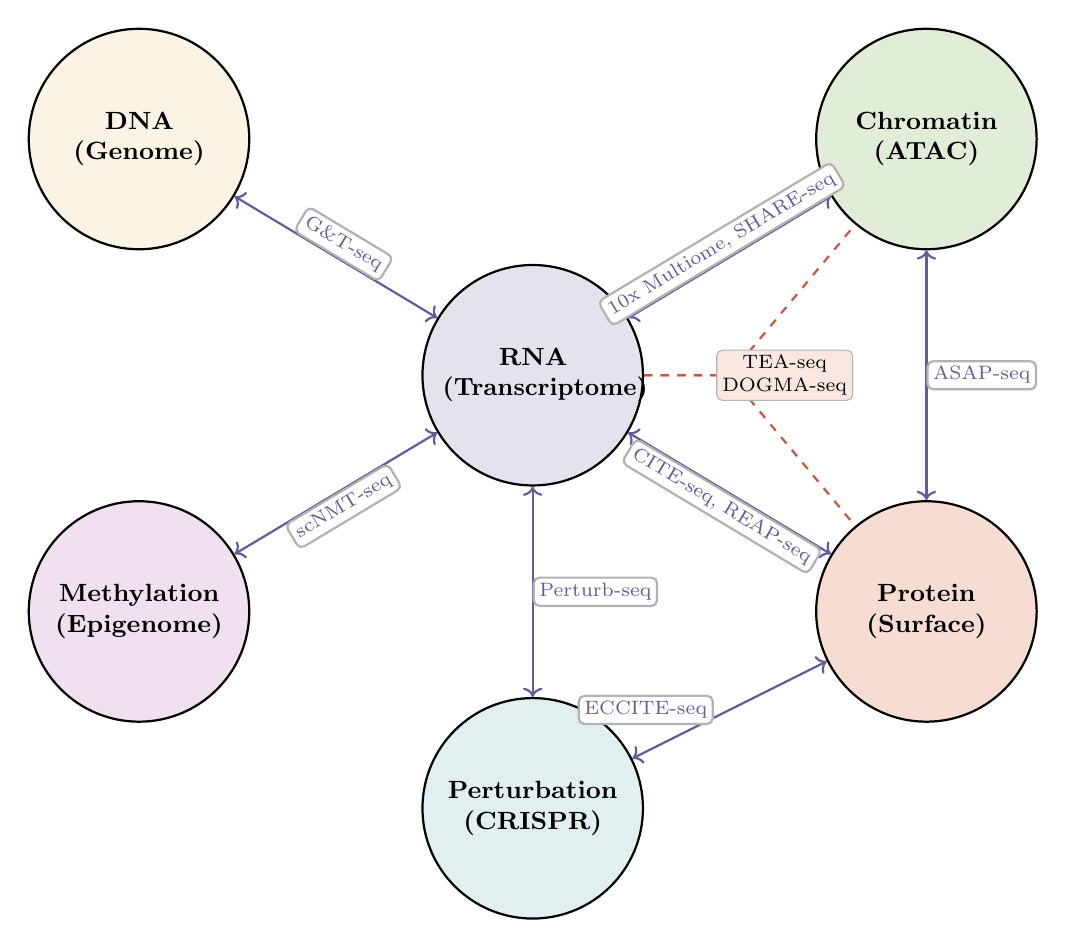
\begin{tikzpicture}[
  modality/.style={
    draw, circle, minimum size=2.8cm, thick,
    font=\small\bfseries, align=center, text width=2.2cm
  },
  method/.style={
    fill=white, draw=gray!60, rounded corners=2pt,
    font=\scriptsize, inner sep=2pt, align=center
  },
  link/.style={thick, MidnightBlue!70, <->},
  triple/.style={thick, BrickRed!70, dashed}
]

% Modality circles
\node[modality, fill=MidnightBlue!12] (rna) at (0,0) {RNA\\(Transcriptome)};
\node[modality, fill=OliveGreen!12] (atac) at (5,3) {Chromatin\\(ATAC)};
\node[modality, fill=BrickRed!12] (protein) at (5,-3) {Protein\\(Surface)};
\node[modality, fill=Goldenrod!12] (dna) at (-5,3) {DNA\\(Genome)};
\node[modality, fill=violet!12] (methyl) at (-5,-3) {Methylation\\(Epigenome)};
\node[modality, fill=teal!12] (perturb) at (0,-5.5) {Perturbation\\(CRISPR)};

% RNA + ATAC links
\draw[link] (rna) -- (atac) node[method, midway, above, sloped] {10x Multiome, SHARE-seq};

% RNA + Protein links
\draw[link] (rna) -- (protein) node[method, midway, below, sloped] {CITE-seq, REAP-seq};

% RNA + DNA links
\draw[link] (rna) -- (dna) node[method, midway, above, sloped] {G\&T-seq};

% RNA + Methylation links
\draw[link] (rna) -- (methyl) node[method, midway, below, sloped] {scNMT-seq};

% ATAC + Protein links
\draw[link] (atac) -- (protein) node[method, midway, right] {ASAP-seq};

% RNA + Perturbation links
\draw[link] (rna) -- (perturb) node[method, midway, right] {Perturb-seq};

% Triple omics (TEA-seq / DOGMA-seq)
\draw[triple] (rna) -- (2.5,0) -- (atac);
\draw[triple] (rna) -- (2.5,0) -- (protein);
\node[method, fill=BrickRed!8] at (3.2,0) {TEA-seq\\DOGMA-seq};

% Protein + Perturbation
\draw[link] (protein) -- (perturb) node[method, midway, left, xshift=-2mm] {ECCITE-seq};

\end{tikzpicture}
\caption[The single-cell multiomics landscape.]{Overview of single-cell multiomics technologies and the molecular modalities they connect. Solid blue arrows indicate dual-modality assays; dashed red lines indicate triple-omics assays. Each technology simultaneously measures the connected modalities from the same individual cell.}
\label{fig:multiomics:landscape}
\end{figure}


\section{Summary}
\label{sec:multiomics:summary}

This chapter has surveyed the rapidly expanding field of single-cell and spatial multiomics. Key takeaways include:

\begin{itemize}[itemsep=3pt]
  \item \textbf{Joint RNA + chromatin:} Technologies such as 10x Multiome and SHARE-seq enable direct linking of regulatory elements to target genes by measuring chromatin accessibility and gene expression in the same cell.
  \item \textbf{Joint RNA + protein:} CITE-seq and related methods provide protein-level cell-type markers alongside whole-transcriptome profiling, bridging the gap between flow cytometry and scRNA-seq.
  \item \textbf{Triple-omics:} TEA-seq and DOGMA-seq achieve simultaneous measurement of RNA, chromatin, and protein, providing the most comprehensive view of single-cell state currently available.
  \item \textbf{Spatial multiomics:} Technologies including spatial-ATAC, CODEX, and DBiT-seq extend multiomics measurements to intact tissues, preserving spatial context.
  \item \textbf{Lineage tracing:} CRISPR barcoding and natural lineage markers (mitochondrial mutations) enable reconstruction of cell lineage trees alongside molecular state.
  \item \textbf{Perturbation screens:} Perturb-seq and CROP-seq map gene function at genome scale by combining CRISPR perturbations with scRNA-seq readout.
  \item \textbf{Computational integration:} The distinction between vertical (same cells), horizontal (same modality), and diagonal (different cells, different modalities) integration is fundamental to choosing appropriate analytical methods.
\end{itemize}

As multiomics technologies continue to mature, their decreasing cost and increasing throughput will make multi-modal profiling the default rather than the exception in single-cell biology, providing an ever more complete picture of cellular identity and function.

\chapter{Specialized Sequencing Applications}
\label{ch:specialized}

\begin{sourcebox}
Ribosome profiling is anchored by its primary report \cite{ingolia2009}. Treatment, nuclease, size-selection, and offset choices can introduce protocol-specific biases, and liquid-biopsy or clinical claims require independent clinical-validation evidence.
\end{sourcebox}

\begin{keyconcept}
Beyond the ``core'' applications of genome sequencing, transcriptomics, and epigenomics, a growing constellation of specialized sequencing assays addresses specific biological questions that standard methods cannot answer. These include ribosome profiling for measuring translation in real time, CRISPR screens for systematic gene function mapping, liquid biopsy for non-invasive cancer detection, epitranscriptomics for profiling RNA modifications, and adaptive nanopore sequencing for software-defined target enrichment. Each represents a creative repurposing of sequencing technology to read a distinct layer of biology.
\end{keyconcept}

\section{Ribosome Profiling (Ribo-seq)}
\label{sec:specialized:riboseq}

\subsection{Principle: Measuring Translation in Real Time}
\label{subsec:specialized:riboseq-principle}

While \acrshort{RNA-seq} measures which genes are transcribed and at what level, it does not reveal which mRNAs are actively being translated into protein. The correlation between mRNA abundance and protein output is notoriously imperfect---post-transcriptional regulation, mRNA stability, and translational control introduce substantial discrepancies. \textbf{Ribosome profiling} (Ribo-seq), developed by Jonathan Weissman and Nicholas Ingolia in 2009, directly measures translation by sequencing the mRNA fragments that are physically protected by actively translating ribosomes.

\begin{protocolbox}[title={Ribo-seq Protocol}]
\begin{enumerate}[itemsep=2pt]
  \item \textbf{Translation arrest:} Treat cells with a translation elongation inhibitor (classically cycloheximide, CHX) to freeze ribosomes in place on their mRNA templates. Alternative inhibitors include lactimidomycin (which captures initiating ribosomes) and harringtonine (which also captures initiation).
  \item \textbf{Cell lysis:} Lyse cells under conditions that preserve ribosome--mRNA complexes.
  \item \textbf{RNase digestion:} Treat the lysate with RNase I (or micrococcal nuclease). This digests all mRNA \textit{not} physically protected by a ribosome, leaving $\sim$28--30 nucleotide (nt) ``footprints'' corresponding to the mRNA segment enclosed within the ribosome's mRNA channel.
  \item \textbf{Ribosome isolation:} Purify monosome-protected fragments by sucrose gradient centrifugation or size-exclusion chromatography.
  \item \textbf{Fragment isolation and library preparation:} Extract the $\sim$28--30\,nt RNA fragments, ligate adapters, reverse-transcribe, and prepare a sequencing library (similar to small RNA library prep).
  \item \textbf{Sequencing:} Single-end sequencing on Illumina (typically SE50 or SE75) yields the identity and position of each ribosome footprint.
  \item \textbf{Parallel RNA-seq:} A matched total RNA or mRNA-seq library is prepared from the same sample to enable calculation of translational efficiency.
\end{enumerate}
\end{protocolbox}

\begin{figure}[htbp]
\centering
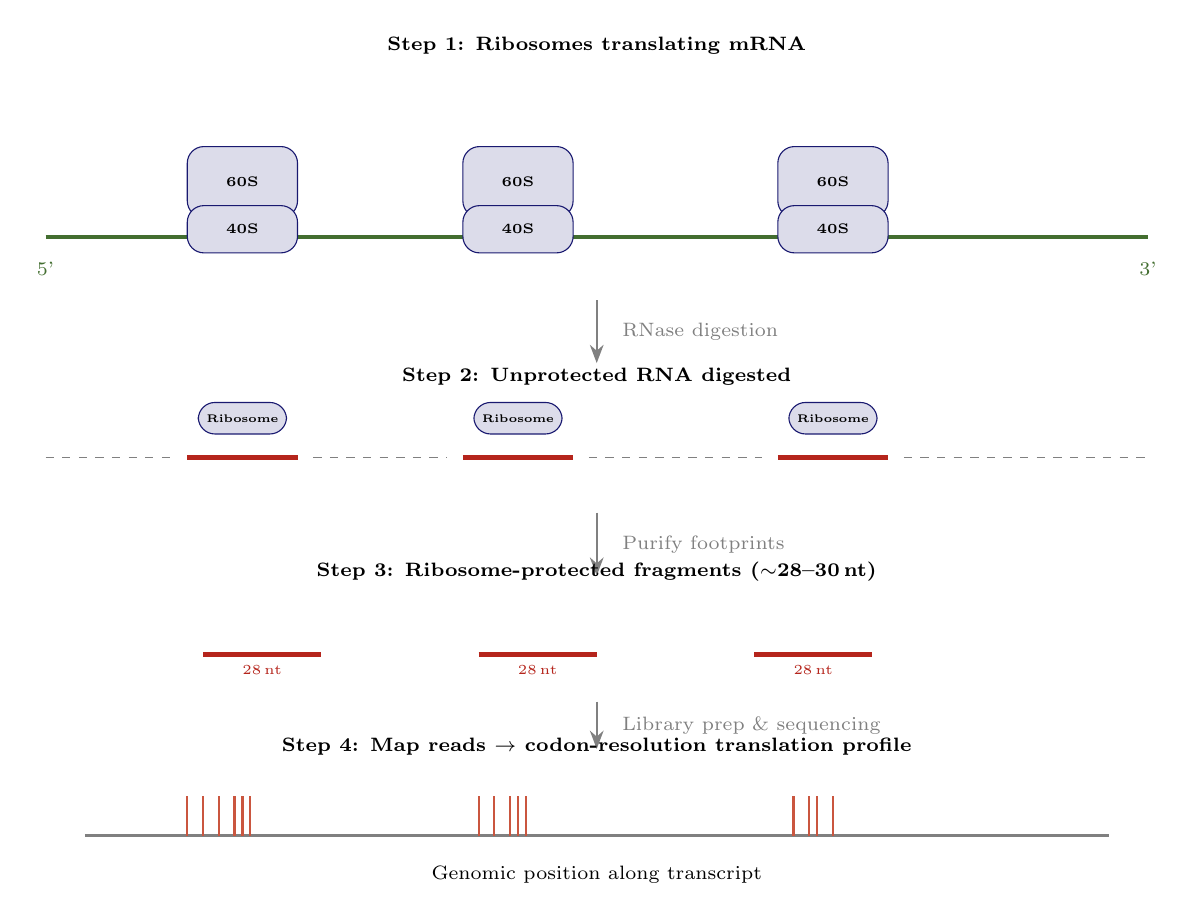
\begin{tikzpicture}[
  >=Stealth,
  ribosome/.style={draw=MidnightBlue, fill=MidnightBlue!15,
    rounded corners=6pt, minimum width=1.4cm, minimum height=0.9cm,
    font=\tiny\bfseries},
  mrna/.style={ultra thick, OliveGreen!80!black},
  footprint/.style={ultra thick, BrickRed},
  label/.style={font=\scriptsize, align=center}
]

% mRNA strand
\draw[mrna] (0,0) -- (14,0);
\node[label, OliveGreen!80!black] at (0,-0.4) {5'};
\node[label, OliveGreen!80!black] at (14,-0.4) {3'};
\node[label, above] at (7,2.2) {\textbf{Step 1: Ribosomes translating mRNA}};

% Ribosomes
\node[ribosome] at (2.5,0.7) {60S};
\node[ribosome, minimum height=0.6cm] at (2.5,0.1) {40S};
\node[ribosome] at (6,0.7) {60S};
\node[ribosome, minimum height=0.6cm] at (6,0.1) {40S};
\node[ribosome] at (10,0.7) {60S};
\node[ribosome, minimum height=0.6cm] at (10,0.1) {40S};

% Arrow to Step 2
\draw[->, thick, gray] (7,-0.8) -- (7,-1.6);
\node[label, gray, right] at (7.2,-1.2) {RNase digestion};

% Step 2: After RNase digestion
\node[label, above] at (7,-2) {\textbf{Step 2: Unprotected RNA digested}};

% Protected footprints only
\draw[footprint] (1.8,-2.8) -- (3.2,-2.8);
\node[ribosome, minimum height=0.5cm, scale=0.8] at (2.5,-2.3) {Ribosome};

\draw[footprint] (5.3,-2.8) -- (6.7,-2.8);
\node[ribosome, minimum height=0.5cm, scale=0.8] at (6,-2.3) {Ribosome};

\draw[footprint] (9.3,-2.8) -- (10.7,-2.8);
\node[ribosome, minimum height=0.5cm, scale=0.8] at (10,-2.3) {Ribosome};

% Digested fragments (dashed)
\draw[gray, dashed, thin] (0,-2.8) -- (1.6,-2.8);
\draw[gray, dashed, thin] (3.4,-2.8) -- (5.1,-2.8);
\draw[gray, dashed, thin] (6.9,-2.8) -- (9.1,-2.8);
\draw[gray, dashed, thin] (10.9,-2.8) -- (14,-2.8);

% Arrow to Step 3
\draw[->, thick, gray] (7,-3.5) -- (7,-4.3);
\node[label, gray, right] at (7.2,-3.9) {Purify footprints};

% Step 3: Footprint fragments
\node[label, above] at (7,-4.5) {\textbf{Step 3: Ribosome-protected fragments ($\sim$28--30\,nt)}};
\draw[footprint] (2,-5.3) -- (3.5,-5.3) node[midway, below, font=\tiny] {28\,nt};
\draw[footprint] (5.5,-5.3) -- (7,-5.3) node[midway, below, font=\tiny] {28\,nt};
\draw[footprint] (9,-5.3) -- (10.5,-5.3) node[midway, below, font=\tiny] {28\,nt};

% Arrow to sequencing
\draw[->, thick, gray] (7,-5.9) -- (7,-6.5);
\node[label, gray, right] at (7.2,-6.2) {Library prep \& sequencing};

% Step 4: Read mapping
\node[label, above] at (7,-6.7) {\textbf{Step 4: Map reads $\rightarrow$ codon-resolution translation profile}};
\draw[gray, thick] (0.5,-7.6) -- (13.5,-7.6);
\foreach \x in {1.8, 2.0, 2.2, 2.4, 2.5, 2.5, 2.6, 5.5, 5.7, 5.9, 6.0, 6.1, 9.5, 9.7, 9.8, 10.0} {
  \draw[BrickRed!70, thick] (\x,-7.6) -- (\x,-7.1);
}
\node[label] at (7,-8.1) {Genomic position along transcript};

\end{tikzpicture}
\caption[Principle of ribosome profiling (Ribo-seq).]{Ribosome profiling (Ribo-seq) captures the $\sim$28--30\,nucleotide mRNA fragments protected by actively translating ribosomes after RNase digestion, providing a snapshot of translation at codon-level resolution.}
\label{fig:specialized:riboseq}
\end{figure}

\subsection{P-site Mapping and Translational Efficiency}
\label{subsec:specialized:riboseq-analysis}

After sequencing, Ribo-seq reads are mapped to the transcriptome. The key analytical concepts are:

\begin{description}[style=nextline, itemsep=3pt]
  \item[P-site assignment] Each ribosome footprint corresponds to a specific codon being decoded. The ``P-site offset'' (typically 12--13\,nt from the 5' end of the footprint for 28-mers) maps each read to the precise codon in the ribosome's peptidyl (P) site. This provides \textbf{codon-level resolution} of translation.

  \item[Three-nucleotide periodicity] Because the ribosome advances three nucleotides (one codon) per step, Ribo-seq data show a characteristic 3-nt periodicity when reads are mapped at single-nucleotide resolution. This periodicity is a hallmark of genuine translation signal and is used as a quality metric.

  \item[Translational efficiency (TE)] Defined as the ratio of ribosome footprint density (RPF) to mRNA abundance:
  \[
  \text{TE}_{\text{gene}} = \frac{\text{RPF}_{\text{gene}} / \text{RPF}_{\text{total}}}{\text{mRNA}_{\text{gene}} / \text{mRNA}_{\text{total}}}
  \]
  Genes with TE $> 1$ are translated more efficiently than average; genes with TE $< 1$ are translationally repressed.
\end{description}

\subsection{P-site Offset Determination and Metagene Analysis}
\label{subsec:specialized:psite-offset}

Accurate assignment of ribosome-protected fragments (RPFs) to the codon being decoded requires careful determination of the \textbf{P-site offset}---the distance from the 5\textquotesingle{} end of the RPF to the codon positioned in the ribosome's peptidyl-transfer (P) site. This offset is not a single fixed value but varies systematically with fragment length.

\begin{keyconcept}[title={Fragment-Length-Dependent P-site Offsets}]
The standard RPF length distribution from eukaryotic ribosomes centres on 28--30\,nt, with minor populations at 20--22\,nt (corresponding to ribosomes in a rotated state). The P-site offset for each fragment length is determined empirically by metagene analysis:

\begin{itemize}[itemsep=2pt]
  \item For \textbf{28-mers}: the P-site offset is typically 12\,nt from the 5\textquotesingle{} end.
  \item For \textbf{29-mers}: the offset is typically 12\,nt.
  \item For \textbf{30-mers}: the offset is typically 13\,nt.
  \item For \textbf{shorter fragments} (20--22\,nt): the offset is typically 9--10\,nt.
\end{itemize}

These values are organism- and protocol-specific and must be calibrated for each experiment.
\end{keyconcept}

The calibration procedure uses \textbf{metagene analysis around annotated start codons}. For a given fragment length $L$, all RPFs of length $L$ whose 5\textquotesingle{} end maps within a window of $\pm 50$\,nt around annotated AUG start codons are aggregated. The P-site offset $\delta_L$ is the displacement from the 5\textquotesingle{} end to the AUG position that produces the sharpest peak. Formally:
\begin{equation}
  \delta_L = \underset{d}{\text{argmax}} \sum_{g \in \mathcal{G}} \text{count}_{L}\bigl(\text{TSS}_g - d\bigr),
  \label{eq:specialized:psite-offset}
\end{equation}
where $\mathcal{G}$ is the set of annotated coding genes, $\text{TSS}_g$ is the position of the AUG start codon for gene $g$, and $\text{count}_{L}(p)$ is the number of RPFs of length $L$ with their 5\textquotesingle{} end at position $p$. The offset $\delta_L$ that maximizes this signal corresponds to the correct P-site assignment for fragments of length $L$.

A complementary analysis uses \textbf{stop codons}: when the P-site offset is correctly assigned, the metagene profile around stop codons should show a sharp drop in RPF density immediately after the stop codon (as ribosomes terminate translation and dissociate). The presence of clear three-nucleotide periodicity throughout the coding sequence, with the majority of P-site-assigned reads falling in the first reading frame (frame 0), serves as the primary quality metric:
\begin{equation}
  F_0 = \frac{\text{RPFs in frame 0}}{\text{RPFs in frame 0} + \text{RPFs in frame 1} + \text{RPFs in frame 2}}.
  \label{eq:specialized:frame-fraction}
\end{equation}
High-quality Ribo-seq datasets typically achieve $F_0 > 0.7$, with the best datasets exceeding 0.9. Tools such as \software{RiboWaltz} and \software{Plastid} automate this calibration process, producing fragment-length-specific offset tables and periodicity plots.

\begin{warningbox}
The choice of translation inhibitor affects the fragment length distribution and P-site offset. Cycloheximide (CHX) pre-treatment produces a broader footprint distribution and can introduce artefacts near start codons due to ribosome run-off during the drug treatment period. Flash-freezing protocols (no drug pre-treatment) or the use of initiation-specific inhibitors (lactimidomycin, harringtonine) produce different footprint profiles. Always calibrate P-site offsets independently for each experimental condition rather than using default values from the literature.
\end{warningbox}

\subsection{Tools for Ribo-seq Analysis}
\label{subsec:specialized:riboseq-tools}

\begin{description}[style=nextline, itemsep=2pt]
  \item[\software{RiboCode}] A Python tool for de novo identification of translated open reading frames (ORFs) based on the 3-nt periodicity signal. Can detect canonical ORFs, upstream ORFs (uORFs), downstream ORFs, and ORFs in long non-coding RNAs.
  \item[\software{ORFquant}] An R package for quantifying translation at the ORF level, distinguishing between multiple ORFs on the same transcript.
  \item[\software{Ribotricer}] Uses a Bayesian changepoint model to detect actively translated ORFs, with particularly good performance on noisy datasets.
  \item[\software{RiboWaltz}] Optimizes P-site offset assignment and provides quality metrics for Ribo-seq data.
\end{description}

\subsection{Discovering Novel Translated ORFs}
\label{subsec:specialized:novel-orfs}

One of the most exciting applications of Ribo-seq is the discovery of previously unannotated translated regions:

\begin{itemize}[itemsep=3pt]
  \item \textbf{Upstream ORFs (uORFs):} Short ORFs in the 5'UTR that are translated before the main coding sequence. uORFs regulate translation of the downstream CDS and are often responsive to stress conditions.
  \item \textbf{Small ORFs (smORFs):} ORFs encoding micropeptides shorter than 100 amino acids, which were historically overlooked by gene annotation pipelines. Ribo-seq has revealed thousands of actively translated smORFs.
  \item \textbf{Alternative reading frames:} Ribo-seq can detect ribosomes translating in unexpected reading frames, including frameshifts.
  \item \textbf{Non-coding RNA translation:} Some annotated ``long non-coding RNAs'' (lncRNAs) show Ribo-seq signal, suggesting they encode short peptides.
\end{itemize}

\begin{warningbox}
Ribo-seq data interpretation requires caution. Cycloheximide pre-treatment can cause run-off of some ribosomes before arrest, introducing artefacts near translation initiation and termination sites. Flash-freezing cells without drug treatment (``flash-freeze'' Ribo-seq) can mitigate this but may introduce other biases. Additionally, the RNase digestion step does not always produce perfectly uniform footprints, and contaminating non-ribosomal RNA fragments (e.g., from RNA-binding protein complexes) can create false signals.
\end{warningbox}


\section{CRISPR Screens}
\label{sec:specialized:crispr-screens}

\subsection{Pooled CRISPR Knockout Screens}
\label{subsec:specialized:crispr-ko}

Pooled CRISPR screens enable systematic loss-of-function studies at genome scale. The principle is to introduce a library of guide RNAs (sgRNAs) targeting every gene in the genome, apply selective pressure, and identify which gene knockouts confer a fitness advantage or disadvantage.

\begin{protocolbox}[title={Pooled CRISPR Knockout Screen Workflow}]
\begin{enumerate}[itemsep=2pt]
  \item \textbf{Library design:} Select a genome-wide sgRNA library (e.g., Brunello library for human, Brie for mouse, each targeting $\sim$20,000 genes with 4 sgRNAs per gene plus $\sim$1,000 non-targeting controls).
  \item \textbf{Library production:} Clone the sgRNA library into a lentiviral backbone containing a selection marker (e.g., puromycin resistance).
  \item \textbf{Cell transduction:} Transduce Cas9-expressing cells at low MOI ($\sim$0.3) to ensure $\sim$90\% of transduced cells carry only one sgRNA. Aim for $\geq$500$\times$ representation (at least 500 cells per sgRNA).
  \item \textbf{Selection:} Apply the selective condition of interest. For a drug resistance screen, treat with the drug; for a fitness screen, simply passage cells for multiple population doublings.
  \item \textbf{Genomic DNA extraction and sgRNA amplification:} Extract gDNA from the surviving cell population and a reference (early timepoint or untreated) population. PCR-amplify the sgRNA cassette from gDNA.
  \item \textbf{Sequencing:} Sequence the sgRNA amplicons on Illumina (typically SE75 or PE75). Only $\sim$20 million reads are needed for a genome-wide library.
  \item \textbf{Analysis:} Count sgRNA reads and compare guide representation between treated and control samples.
\end{enumerate}
\end{protocolbox}

\subsection{CRISPRi and CRISPRa Screens}
\label{subsec:specialized:crispri-crispra}

\begin{description}[style=nextline, itemsep=3pt]
  \item[CRISPRi (CRISPR interference)] Uses a catalytically dead Cas9 (dCas9) fused to a transcriptional repressor domain (KRAB). The sgRNA directs dCas9 to the target gene's promoter, where KRAB silences transcription without cutting DNA. Advantages over CRISPRko: no DNA damage response, titratable repression, reversible.

  \item[CRISPRa (CRISPR activation)] Uses dCas9 fused to transcriptional activator domains (e.g., VP64, p65, Rta in the ``VPR'' system, or the synergistic activation mediator SAM system). This enables gain-of-function screens that complement loss-of-function approaches. CRISPRa guides target promoter regions to upregulate endogenous gene expression.
\end{description}

\subsection{Guide RNA Library Design}
\label{subsec:specialized:sgrna-design}

Effective sgRNA design is critical for screen success. Key considerations include:

\begin{itemize}[itemsep=2pt]
  \item \textbf{On-target efficiency:} Algorithms such as Rule Set 2 (Doench et al.) and DeepCas9 predict sgRNA cutting efficiency based on sequence features.
  \item \textbf{Off-target effects:} Tools such as CRISPRscan, Cas-OFFinder, and GuideScan rank guides by predicted specificity.
  \item \textbf{Target location:} For CRISPRko, guides targeting early constitutive exons are most effective. For CRISPRi/a, guides near the transcription start site (TSS) are optimal ($-$50 to $+$300\basepair{} for CRISPRi; $-$400 to $-$50\basepair{} for CRISPRa).
  \item \textbf{Controls:} Include non-targeting controls (guides with no match in the genome), safe-harbour targeting controls (guides targeting inert genomic loci), and positive controls (guides targeting known essential or drug-target genes).
\end{itemize}

\subsection{Analysis Tools for CRISPR Screens}
\label{subsec:specialized:crispr-tools}

\begin{description}[style=nextline, itemsep=2pt]
  \item[\software{MAGeCK} (Model-based Analysis of Genome-wide CRISPR-Cas9 Knockout)] The most widely used tool. MAGeCK uses a negative binomial model to identify sgRNAs with significantly altered abundance, then aggregates sgRNA-level results to gene-level scores using robust rank aggregation (RRA) or maximum likelihood estimation (MLE). MAGeCK-VISPR provides a visualization platform.

  \item[\software{BAGEL2} (Bayesian Analysis of Gene Essentiality with Location)] Calculates a Bayes Factor for each gene, representing the likelihood that the gene is essential vs.\ non-essential, using reference sets of known essential and non-essential genes.

  \item[\software{CRISPRcleanR}] Corrects for copy-number-dependent sgRNA depletion bias that can confound screen results in aneuploid cell lines (common in cancer cells).
\end{description}

\subsection{MAGeCK Statistical Framework}
\label{subsec:specialized:mageck-model}

\software{MAGeCK} (Model-based Analysis of Genome-wide CRISPR-Cas9 Knockout) is the most widely used statistical framework for analysing pooled CRISPR screen data. Its two-stage approach---sgRNA-level modelling followed by gene-level aggregation---provides robust identification of screen hits even in the presence of variable sgRNA efficiency and noisy count data.

\subsubsection{sgRNA-Level Negative Binomial Model}

For each sgRNA $j$, MAGeCK models the read count $Y_{jc}$ in condition $c$ (treatment or control) using a \textbf{negative binomial} (NB) distribution:
\begin{equation}
  Y_{jc} \sim \text{NB}(\mu_{jc},\; \alpha_j),
  \label{eq:specialized:mageck-nb}
\end{equation}
where $\mu_{jc}$ is the expected count for sgRNA $j$ in condition $c$, and $\alpha_j$ is the sgRNA-specific dispersion parameter. The mean $\mu_{jc}$ is modelled as:
\begin{equation}
  \mu_{jc} = s_c \cdot \mu_{j0} \cdot 2^{\beta_j},
  \label{eq:specialized:mageck-mean}
\end{equation}
where $s_c$ is a sample-specific size factor (estimated by median-ratio normalization), $\mu_{j0}$ is the baseline mean count for sgRNA $j$, and $\beta_j$ is the log$_2$ fold change for sgRNA $j$ between treatment and control. The negative binomial model accounts for both Poisson sampling noise and biological overdispersion---the latter arising from stochastic variation in lentiviral integration, cell growth, and PCR amplification.

The dispersion parameter $\alpha_j$ is estimated using a mean-variance relationship: MAGeCK fits a smooth curve $\hat{\alpha}(\mu)$ relating the variance to the mean across all sgRNAs, then uses this curve as an empirical Bayes prior to regularize per-sgRNA dispersion estimates. This borrowing of information across sgRNAs stabilizes estimation for low-count guides.

A $p$-value for each sgRNA is obtained by testing $H_0: \beta_j = 0$ against the appropriate one-sided alternative (depletion or enrichment), using the NB likelihood ratio test or Wald test.

\subsubsection{Gene-Level Aggregation via Robust Rank Aggregation}

Because each gene is targeted by multiple sgRNAs (typically 4--10), MAGeCK aggregates sgRNA-level evidence to the gene level using \textbf{Robust Rank Aggregation} (RRA). For each gene $g$ targeted by sgRNAs $\{j_1, j_2, \ldots, j_{n_g}\}$:

\begin{enumerate}[itemsep=2pt]
  \item Rank all sgRNAs in the library by their $p$-values (from the NB test).
  \item Extract the normalized ranks $r_{j_1}, r_{j_2}, \ldots, r_{j_{n_g}}$ for the sgRNAs targeting gene $g$, where each rank is divided by the total number of sgRNAs to obtain a value in $[0, 1]$.
  \item Under the null hypothesis (gene $g$ has no effect), these normalized ranks are uniformly distributed on $[0,1]$. The RRA score for gene $g$ is based on the minimum-order-statistic $p$-value:
  \begin{equation}
    \rho_g = \min_{k=1,\ldots,n_g} \; \beta_{\text{min}}\bigl(r_{g(k)};\, k,\, n_g - k + 1\bigr),
    \label{eq:specialized:rra}
  \end{equation}
  where $r_{g(k)}$ is the $k$-th smallest normalized rank among the sgRNAs targeting gene $g$, and $\beta_{\text{min}}(\cdot; a, b)$ is the CDF of the $k$-th order statistic from a $\text{Uniform}(0,1)$ sample, which follows a Beta$(k, n_g - k + 1)$ distribution.
  \item The RRA score $\rho_g$ represents the probability of observing ranks as extreme as those of gene $g$'s sgRNAs by chance. Lower scores indicate stronger evidence that the gene is a screen hit.
\end{enumerate}

\begin{keyconcept}[title={Why RRA Is Robust}]
The power of RRA lies in its robustness to individual sgRNA failure. A gene is called significant even if one or two of its sgRNAs show no effect (due to poor cutting efficiency or off-target integration), as long as the remaining sgRNAs show consistent enrichment or depletion. This is critical because sgRNA efficiency varies substantially, and requiring all guides to show an effect would dramatically reduce sensitivity. The $\alpha$-RRA variant (used by default in MAGeCK) further improves robustness by only considering the top $\alpha$ fraction of sgRNAs per gene, discarding obvious non-functional guides.
\end{keyconcept}

MAGeCK also provides a \textbf{maximum likelihood estimation} (MLE) module for more complex experimental designs (e.g., multiple conditions, time series, paired samples), which jointly estimates gene-level effect sizes within a generalized linear model framework. The MLE module models the mean count for sgRNA $j$ in sample $c$ as:
\begin{equation}
  \log \mu_{jc} = \log s_c + \beta_0 + \beta_{g(j)} \cdot d_c,
  \label{eq:specialized:mageck-mle}
\end{equation}
where $\beta_0$ is the baseline, $\beta_{g(j)}$ is the gene-level effect size for the gene targeted by sgRNA $j$, and $d_c$ is the design matrix entry for sample $c$. This formulation allows multi-factor designs including drug treatment, time course, and interaction effects.

\begin{table}[htbp]
\centering
\caption[Comparison of CRISPR screen analysis tools.]{Comparison of statistical frameworks for pooled CRISPR screen analysis.}
\label{tab:specialized:crispr-tools-comparison}
\small
\begin{tabularx}{\textwidth}{>{\bfseries\raggedright}p{2.0cm} X c c}
\toprule
\textbf{Tool} & \textbf{Statistical Model} & \textbf{Multi-condition} & \textbf{Copy-number correction} \\
\midrule
MAGeCK-RRA & Negative binomial + Robust Rank Aggregation & No & No \\
\addlinespace
MAGeCK-MLE & Negative binomial GLM with gene-level effects & Yes & No \\
\addlinespace
BAGEL2 & Bayes Factor using essential/non-essential reference sets & No & No \\
\addlinespace
CRISPRcleanR & Unsupervised segmentation to correct CN bias & No & Yes \\
\addlinespace
JACKS & Joint Analysis of CRISPR/Cas9 Knockout Screens & Yes (multi-replicate) & No \\
\bottomrule
\end{tabularx}
\end{table}

\begin{tipbox}[title={Genome-wide vs.\ Focused Screens}]
Genome-wide screens ($\sim$80,000--100,000 sgRNAs for human) require large cell numbers ($>$50 million cells for 500$\times$ representation at MOI 0.3) and are best suited for unbiased discovery. Focused screens targeting specific gene sets (e.g., kinases, transcription factors, drug targets) can be performed with fewer cells, more sgRNAs per gene, and deeper sequencing, yielding higher statistical power for the genes included. Consider your biological question when choosing between the two approaches.
\end{tipbox}


\section{Cell-Free DNA and Liquid Biopsy}
\label{sec:specialized:cfdna}

\subsection{Circulating Tumor DNA (ctDNA)}
\label{subsec:specialized:ctdna}

Cell-free DNA (cfDNA) consists of short DNA fragments circulating in the bloodstream, released primarily by apoptotic and necrotic cells. In healthy individuals, cfDNA is predominantly derived from hematopoietic cells. In cancer patients, a fraction of cfDNA originates from tumour cells---this fraction is called \textbf{circulating tumour DNA (ctDNA)}.

Key characteristics of cfDNA:
\begin{itemize}[itemsep=2pt]
  \item Fragment size peaks at $\sim$167\basepair{}, corresponding to one nucleosome of wrapped DNA ($\sim$147\basepair{}) plus linker DNA ($\sim$20\basepair{}). A secondary peak at $\sim$334\basepair{} (dinucleosomal) is often observed.
  \item ctDNA fraction varies enormously: from $>$50\% in advanced metastatic cancers to $<$0.01\% in early-stage cancers.
  \item ctDNA carries the same somatic mutations, copy number alterations, and methylation patterns as the tumour of origin.
\end{itemize}

\subsection{Non-Invasive Prenatal Testing (NIPT)}
\label{subsec:specialized:nipt}

NIPT was the first clinical application of cfDNA sequencing. Cell-free fetal DNA (cffDNA), shed from the placenta into the maternal bloodstream, represents $\sim$5--20\% of total maternal cfDNA from approximately 10 weeks of gestation. By shallow whole-genome sequencing ($\sim$0.1--0.5$\times$ coverage) of maternal plasma cfDNA, chromosomal aneuploidies in the fetus (trisomy 21, 18, 13) can be detected as subtle shifts in the proportion of reads mapping to the affected chromosome.

\begin{keyconcept}[title={NIPT Statistical Principle}]
If the fetus has trisomy 21, chromosome 21 constitutes a slightly larger fraction of total cfDNA than expected (because the placenta sheds three copies instead of two). With sufficient sequencing depth, this excess---on the order of a few percent of the fetal fraction---can be detected statistically. The higher the fetal fraction, the more reliable the test. This is why NIPT is typically performed after 10 weeks of gestation, when fetal fraction is sufficient.
\end{keyconcept}

\subsection{Cancer Detection Applications}
\label{subsec:specialized:cancer-detection}

\begin{description}[style=nextline, itemsep=3pt]
  \item[Multi-cancer early detection (MCED)] The GRAIL Galleri test uses cfDNA methylation patterns (rather than mutations) to detect over 50 cancer types from a single blood draw, with the ability to predict the tissue of origin. The test sequences cfDNA after methylation-sensitive enrichment and uses a machine learning classifier trained on thousands of cancer and non-cancer samples.

  \item[Minimal residual disease (MRD)] After cancer treatment (surgery, chemotherapy), ctDNA monitoring can detect residual disease months before imaging detects recurrence. Tumor-informed assays (e.g., Signatera by Natera) design patient-specific panels based on the tumour's mutation profile, achieving sensitivity to detect ctDNA fractions as low as $\sim$0.001\%.

  \item[Treatment monitoring] Serial ctDNA quantification tracks treatment response in real time. Rising ctDNA levels during therapy indicate treatment failure before clinical or imaging progression.
\end{description}

\subsection{Fragmentomics}
\label{subsec:specialized:fragmentomics}

The fragmentation pattern of cfDNA carries biological information beyond the sequence itself:

\begin{description}[style=nextline, itemsep=3pt]
  \item[Fragment size distribution] Tumour-derived cfDNA fragments tend to be slightly shorter than normal cfDNA. Fragment size profiling can enhance ctDNA detection.

  \item[DELFI (DNA Evaluation of Fragments for early Interception)] Analyses genome-wide fragmentation patterns (the ratio of short to long fragments in 5\megabase{} bins) to detect cancer. The rationale is that altered chromatin organization in cancer cells produces distinct fragmentation patterns when DNA is released into the blood.

  \item[Nucleosome positioning] cfDNA fragments reflect the nucleosome landscape of their cell of origin. Regions protected by nucleosomes produce fragments, while nucleosome-free regions (e.g., active promoters) are depleted. This can be used to infer gene expression and cell-of-origin from cfDNA.
\end{description}

\subsection{cfDNA Fragmentomics: From Size Distributions to Nucleosome Footprinting}
\label{subsec:specialized:fragmentomics-detail}

The fragmentation pattern of cfDNA encodes substantial biological information that extends far beyond simple tumour detection. Understanding the biophysical basis of cfDNA fragmentation is essential for interpreting fragmentomic data.

\subsubsection{Nucleosomal Fragment Size Distribution}

cfDNA fragments are not randomly sized. Their length distribution reflects the nucleosomal organization of the chromatin in the cells of origin. The dominant peak at $\sim$167\basepair{} corresponds to the \textbf{mono-nucleosomal unit}: 147\basepair{} of DNA wrapped around a histone octamer plus $\sim$20\basepair{} of linker DNA protected by histone H1. Subsequent peaks at $\sim$334\basepair{} (di-nucleosomal) and $\sim$501\basepair{} (tri-nucleosomal) represent fragments spanning two and three nucleosomes, respectively.

Within the mono-nucleosomal peak, finer structure is apparent in high-depth sequencing data:
\begin{itemize}[itemsep=2pt]
  \item A \textbf{sub-nucleosomal peak at $\sim$145\basepair{}} corresponds to the nucleosome core particle without linker DNA, observed when H1 is absent or displaced.
  \item Fragments shorter than 145\basepair{} ($\sim$80--120\basepair{}) likely arise from nucleosome remodelling events or represent DNA protected by non-histone protein complexes (e.g., transcription factors).
  \item A 10\basepair{} periodicity within the mono-nucleosomal peak reflects the helical pitch of DNA on the nucleosome surface, with preferential cleavage occurring where the minor groove faces outward.
\end{itemize}

\subsubsection{Nucleosome Footprinting of Transcription Factor Binding}

At genomic regions bound by transcription factors in the cells of origin, cfDNA shows characteristic \textbf{nucleosome depletion}---a reduction in fragment coverage centred on the TF binding site, flanked by well-positioned nucleosomes that produce phased fragment ends. This pattern enables inference of TF binding activity and, by extension, the cell type of origin from cfDNA data alone.

The nucleosome footprinting approach works as follows:
\begin{enumerate}[itemsep=2pt]
  \item Align cfDNA reads to the reference genome and extract fragment start/end positions.
  \item For each known TF binding site (from databases such as ENCODE or JASPAR), aggregate the coverage of cfDNA fragment midpoints in a window around the site.
  \item Sites actively bound by TFs in the cells of origin show a characteristic ``V-shaped'' depletion profile, while unbound sites show uniform nucleosomal coverage.
  \item By comparing the depth of the nucleosome-free region across thousands of TF binding sites, one can infer which TFs are active in the cells contributing cfDNA to the plasma.
\end{enumerate}

\subsubsection{ctDNA Detection Sensitivity}

The sensitivity of ctDNA detection depends on two key parameters: the \textbf{tumour fraction} $f$ (the proportion of cfDNA molecules derived from the tumour) and the \textbf{sequencing depth} $N$ (the number of unique cfDNA molecules sampled). For a given somatic mutation present in the tumour, the expected number of mutant molecules in a cfDNA sample is $n_{\text{mut}} = f \cdot N$. To detect a mutation with confidence, one requires $n_{\text{mut}}$ to exceed the background error rate of the assay.

For standard Illumina sequencing (error rate $\epsilon \approx 10^{-3}$), the limit of detection is approximately $f \geq 1\%$. With UMI-based error correction ($\epsilon \approx 10^{-5}$), detection extends to $f \geq 0.01\%$. With duplex sequencing ($\epsilon \approx 10^{-7}$), even lower tumour fractions become theoretically accessible, though the number of unique molecules sampled becomes the limiting factor.

The probability of detecting at least one mutant molecule follows a binomial model:
\begin{equation}
  P(\text{detect}) = 1 - (1 - f)^{N} \approx 1 - e^{-fN}, \quad \text{for small } f,
  \label{eq:specialized:ctdna-sensitivity}
\end{equation}
which shows that for a tumour fraction of $f = 0.01\%$, one needs to sample $N \geq 30{,}000$ unique molecules to achieve $>$95\% probability of observing at least one mutant molecule. In practice, achieving this many unique molecules requires deep sequencing (typically $>$50{,}000$\times$ raw coverage, reduced to $\sim$30{,}000$\times$ unique coverage after UMI deduplication) or enrichment for the target locus using hybrid capture panels.

\begin{tipbox}[title={Tumour-Informed vs.\ Tumour-Agnostic Assays}]
Tumour-informed assays (e.g., Signatera, Archer) design patient-specific panels targeting mutations identified from the primary tumour, achieving higher sensitivity by interrogating known variants. Tumour-agnostic assays (e.g., Guardant360, FoundationOne Liquid CDx) use fixed panels of cancer-associated genes, sacrificing some sensitivity for broader applicability when tumour tissue is unavailable. For minimal residual disease (MRD) monitoring, tumour-informed assays can detect ctDNA at fractions as low as $\sim$0.001\%, while tumour-agnostic panels typically require $\geq$0.1\% tumour fraction.
\end{tipbox}

\subsection{Methylation-Based Cancer Detection}
\label{subsec:specialized:cfmedip}

\textbf{cfMeDIP-seq} (cell-free Methylated DNA ImmunoPrecipitation sequencing) uses an antibody against 5-methylcytosine to enrich methylated cfDNA fragments, followed by sequencing. Because DNA methylation patterns are highly cell-type-specific and extensively reprogrammed in cancer, methylation-based approaches can both detect cancer and identify the tissue of origin.

\subsection{Technical Challenges and Error Correction}
\label{subsec:specialized:error-correction}

Detecting rare ctDNA variants (at allele fractions below 1\%) requires error rates far below standard Illumina sequencing ($\sim$0.1\% per base). Two key strategies address this:

\begin{description}[style=nextline, itemsep=3pt]
  \item[\acrshort{UMI}-based error correction] Unique molecular identifiers (UMIs) are ligated to each original DNA molecule before amplification. After sequencing, reads sharing the same UMI are grouped into ``families'' derived from the same original molecule. Errors introduced during PCR or sequencing will appear in only some family members, while true variants will be present in all. Consensus calling across UMI families suppresses errors by several orders of magnitude.

  \item[Duplex sequencing] Tags both strands of the original DNA duplex with complementary UMIs, so that reads from the Watson and Crick strands can be identified. A true mutation must be present on \textit{both} strands; PCR errors or sequencing errors will appear on only one strand. This achieves error rates approaching $10^{-7}$ per base---the lowest of any sequencing method.
\end{description}

\begin{keyconcept}[title={Duplex Sequencing}]
Duplex sequencing achieves the lowest error rate of any sequencing approach ($\sim$$10^{-7}$ per base) by requiring that a variant be present on both complementary strands of the original DNA molecule. This is mathematically equivalent to requiring two independent mutations at the same position---an extraordinarily unlikely event. Applications include ultra-rare variant detection, somatic mutagenesis studies (measuring mutation rates in normal tissues), and forensic DNA analysis.
\end{keyconcept}


\section{Adaptive Sampling (Oxford Nanopore)}
\label{sec:specialized:adaptive}

\subsection{Real-Time Selective Sequencing}
\label{subsec:specialized:adaptive-principle}

One of the most distinctive capabilities of Oxford Nanopore sequencing is \textbf{adaptive sampling} (also called ``Read Until''): the ability to selectively sequence specific genomic regions in real time, \textit{without any physical enrichment or capture step}. The principle is elegantly simple:

\begin{enumerate}[itemsep=2pt]
  \item A DNA molecule enters a nanopore and begins translocating.
  \item The first few hundred bases of the molecule are sequenced and mapped in real time against a reference genome.
  \item If the molecule maps to a region of interest, translocation continues and the full read is collected.
  \item If the molecule maps to an off-target region, the pore voltage is reversed, ejecting the molecule and making the pore available for a new molecule.
\end{enumerate}

This software-defined enrichment achieves $\sim$2--5$\times$ enrichment for target regions relative to random sequencing, without any wet-lab modification to the library preparation.

\subsection{Software and Applications}
\label{subsec:specialized:adaptive-software}

\begin{description}[style=nextline, itemsep=3pt]
  \item[\software{ReadFish}] A Python framework for real-time adaptive sampling that integrates with the MinKNOW acquisition software. Users specify target regions as BED files, and ReadFish handles the real-time basecalling, mapping, and accept/reject decisions.

  \item[\software{MinKNOW adaptive sampling}] ONT's built-in adaptive sampling feature, available directly in the MinKNOW software without additional tools.

  \item[Applications] Adaptive sampling is particularly valuable for:
  \begin{itemize}[itemsep=2pt]
    \item Targeted sequencing of specific genes or regions without capture probes.
    \item Pathogen enrichment from clinical metagenomic samples (accept pathogen reads, reject host reads).
    \item Human host depletion (reject human reads to enrich for microbial sequences).
    \item Selective sequencing of specific chromosomes or genomic regions of interest.
  \end{itemize}
\end{description}

\begin{tipbox}
Adaptive sampling works best for applications where the target represents a minority of the total DNA. If the target is $>$50\% of the genome, there is no enrichment benefit. The enrichment factor also depends on read length: longer molecules have higher mapping confidence from the initial fragment, enabling more accurate accept/reject decisions. Use long DNA extraction protocols ($>$10\kilobase{} fragment length) for optimal adaptive sampling performance.
\end{tipbox}


\section{Optical Genome Mapping (Bionano Saphyr)}
\label{sec:specialized:ogm}

Optical genome mapping (OGM) is not sequencing in the traditional sense, but it is an increasingly important complement to sequencing for structural variant (SV) detection. The Bionano Saphyr platform works by:

\begin{enumerate}[itemsep=2pt]
  \item Extracting ultra-high molecular weight DNA (molecules $>$150\kilobase{}, ideally $>$250\kilobase{}).
  \item Labelling the DNA at specific sequence motifs (typically the 6-bp motif CTTAAG) with fluorescent tags using the DLE-1 enzyme.
  \item Linearizing the labelled molecules in nanochannel arrays and imaging the fluorescent label pattern.
  \item Comparing the observed label pattern to the expected pattern from a reference genome to detect structural variants.
\end{enumerate}

OGM is particularly powerful for detecting:
\begin{itemize}[itemsep=2pt]
  \item Large structural variants ($>$500\basepair{}) including deletions, duplications, inversions, and translocations.
  \item Complex rearrangements in cancer genomes and constitutional chromosomal abnormalities.
  \item Repeat expansions (e.g., in trinucleotide repeat disorders such as Friedreich's ataxia, Fragile X syndrome).
  \item Balanced translocations that are invisible to short-read sequencing and copy-number arrays.
\end{itemize}

\begin{warningbox}
OGM does not provide nucleotide-level sequence information. It detects structural variants based on label pattern disruption, but it cannot resolve the exact breakpoint sequence. For full characterization, OGM findings should be confirmed and refined by long-read sequencing or targeted PCR and Sanger sequencing of breakpoint junctions.
\end{warningbox}


\section{Epitranscriptomics: RNA Modifications}
\label{sec:specialized:epitranscriptomics}

\subsection{The RNA Modification Landscape}
\label{subsec:specialized:rna-mods}

Just as DNA is chemically modified (methylation, hydroxymethylation), RNA carries over 170 known chemical modifications that regulate its function. The most abundant and well-studied modifications in mRNA include:

\begin{description}[style=nextline, itemsep=3pt]
  \item[N$^6$-methyladenosine (m$^6$A)] The most abundant internal modification in eukaryotic mRNA. Found predominantly near stop codons and in 3'UTRs. Regulated by ``writer'' enzymes (METTL3/METTL14 complex), ``eraser'' enzymes (FTO, ALKBH5), and ``reader'' proteins (YTHDF1/2/3, YTHDC1/2). Influences mRNA stability, splicing, translation efficiency, and nuclear export.

  \item[5-methylcytosine (m$^5$C)] Found in both mRNA and tRNA. Written by NSUN2 and DNMT2. Implicated in mRNA stability and nuclear--cytoplasmic export.

  \item[Pseudouridine ($\Psi$)] The most abundant RNA modification overall (highly prevalent in rRNA and tRNA). In mRNA, $\Psi$ can affect translation fidelity and mRNA stability. Detected by $\Psi$-seq or bisulfite-based methods.

  \item[N$^1$-methyladenosine (m$^1$A)] Found in tRNA and rRNA; less common in mRNA. m$^1$A in the 5'UTR may promote cap-independent translation under stress conditions.
\end{description}

\subsection{Sequencing-Based Detection of RNA Modifications}
\label{subsec:specialized:rna-mod-detection}

\begin{description}[style=nextline, itemsep=3pt]
  \item[MeRIP-seq / m$^6$A-seq] The most widely used method for transcriptome-wide m$^6$A mapping. mRNA is fragmented ($\sim$100\,nt), immunoprecipitated with an anti-m$^6$A antibody, and sequenced. Enriched regions (``m$^6$A peaks'') are identified by comparing IP to input libraries. Resolution is limited to $\sim$100--200\,nt (the fragment size).

  \item[miCLIP (m$^6$A individual-nucleotide-resolution cross-linking and immunoprecipitation)] Achieves single-nucleotide resolution by UV cross-linking the anti-m$^6$A antibody to the RNA, creating characteristic mutation signatures at the cross-link site.

  \item[DART-seq (Deamination Adjacent to RNA modification Targets)] An antibody-free approach that fuses the m$^6$A-binding YTH domain to the cytidine deaminase APOBEC1. The fusion protein binds m$^6$A sites and deaminates nearby cytidines to uridines, creating C-to-U mutations detectable by standard RNA-seq. DART-seq requires much less input RNA than MeRIP-seq.

  \item[MAZTER-seq] Exploits the m$^6$A-sensitive RNase MazF, which cleaves at unmethylated ACA motifs but not at methylated m$^6$AACA motifs. Methylated sites appear as uncleaved positions in the sequencing data.

  \item[Direct nanopore detection] Oxford Nanopore direct RNA sequencing can detect RNA modifications in native RNA without any chemical treatment. The modifications alter the electrical signal as the RNA translocates through the pore. Computational tools (\software{m6Anet}, \software{ELIGOS}, \software{Nanom6A}) use neural networks to classify modified vs.\ unmodified bases from the raw signal. This is the only method that preserves the full-length transcript context and avoids all biochemical biases.
\end{description}

\begin{warningbox}
MeRIP-seq/m$^6$A-seq has significant limitations: low resolution ($\sim$100--200\,nt), high input requirements ($>$5\,$\mu$g poly-A+ RNA), antibody cross-reactivity (the anti-m$^6$A antibody can also bind m$^6$Am, the cap-adjacent modification), and batch-dependent variability. Results should be validated with orthogonal methods (e.g., miCLIP, DART-seq, or site-specific qPCR after SELECT) before drawing strong biological conclusions.
\end{warningbox}


\section{Telomere and Centromere Sequencing: T2T Approaches}
\label{sec:specialized:t2t}

The Telomere-to-Telomere (T2T) Consortium completed the first truly complete human genome assembly in 2022, filling in the $\sim$8\% of the genome (nearly 200\megabase{}) that was missing from the GRCh38 reference. This achievement was enabled by:

\begin{itemize}[itemsep=2pt]
  \item \textbf{Ultra-long nanopore reads} ($>$100\kilobase{}) that spanned centromeric satellite repeats.
  \item \textbf{PacBio HiFi reads} that provided the high accuracy needed for consensus polishing.
  \item The use of a complete hydatidiform mole cell line (CHM13), which is effectively haploid, eliminating the challenge of separating homologous chromosomes.
\end{itemize}

The T2T-CHM13 assembly revealed complete centromere structures (megabases of alpha-satellite repeats), full-length ribosomal DNA arrays, segmental duplications, and hundreds of previously missing protein-coding genes. Assembling telomeric and centromeric regions remains challenging even with current long-read technology, requiring specialized assembly algorithms (e.g., \software{verkko}) and careful manual curation.


\section{Chromosome Conformation in Clinical Settings}
\label{sec:specialized:clinical-hic}

While Hi-C and related chromosome conformation capture methods were originally research tools, they are increasingly entering clinical settings, particularly for:

\begin{itemize}[itemsep=2pt]
  \item \textbf{Structural variant detection:} Hi-C data intrinsically detect inter-chromosomal translocations (visible as off-diagonal contact signal) and large-scale inversions (visible as altered contact patterns), including balanced rearrangements that are invisible to copy-number arrays.
  \item \textbf{Haplotype phasing:} Hi-C links distant genomic loci that reside on the same chromosome, enabling chromosome-scale haplotype phasing.
  \item \textbf{Cancer karyotyping:} Hi-C-based approaches (e.g., from Arima Genomics or Phase Genomics) can replace traditional cytogenetic karyotyping for detecting chromosomal rearrangements in haematological malignancies.
\end{itemize}


\section{Practical Workflow: Ribo-seq Processing}
\label{sec:specialized:riboseq-workflow}

\subsection{Snakemake Workflow}
\label{subsec:specialized:riboseq-snakemake}

\begin{lstlisting}[language=Python, caption={Snakemake workflow for Ribo-seq analysis.}, label={lst:specialized:riboseq-snakemake}]
# Snakefile for Ribo-seq Analysis Pipeline
configfile: "config/riboseq_config.yaml"

SAMPLES = config["samples"]
GENOME = config["genome_fasta"]
ANNOTATION = config["gtf"]
RRNA_INDEX = config["rrna_bowtie2_index"]
STAR_INDEX = config["star_index"]

rule all:
    input:
        expand("results/{sample}/ribocode/"
               "ORF_result.txt", sample=SAMPLES),
        expand("results/{sample}/translational_efficiency.tsv",
               sample=SAMPLES),
        "results/qc/multiqc_report.html"

rule trim_adapters:
    """Trim adapters from Ribo-seq reads."""
    input:
        fastq="data/{sample}.fastq.gz"
    output:
        trimmed="results/{sample}/trimmed/{sample}.fastq.gz"
    threads: 4
    shell:
        """
        cutadapt -a AGATCGGAAGAGCACACGTCT \
            --minimum-length 20 --maximum-length 35 \
            -j {threads} \
            -o {output.trimmed} {input.fastq}
        """

rule remove_rrna:
    """Remove rRNA contamination with Bowtie2."""
    input:
        fastq="results/{sample}/trimmed/{sample}.fastq.gz"
    output:
        non_rrna="results/{sample}/filtered/"
                 "{sample}_no_rrna.fastq.gz",
        rrna_log="results/{sample}/filtered/rrna_stats.txt"
    params:
        index=RRNA_INDEX
    threads: 8
    shell:
        """
        bowtie2 -x {params.index} \
            -U {input.fastq} \
            --un-gz {output.non_rrna} \
            -p {threads} --very-sensitive \
            -S /dev/null \
            2> {output.rrna_log}
        """

rule star_align:
    """Align to genome/transcriptome with STAR."""
    input:
        fastq="results/{sample}/filtered/"
              "{sample}_no_rrna.fastq.gz"
    output:
        bam="results/{sample}/aligned/"
            "{sample}_Aligned.toTranscriptome.out.bam",
        genome_bam="results/{sample}/aligned/"
                   "{sample}_Aligned.sortedByCoord.out.bam"
    params:
        index=STAR_INDEX,
        prefix="results/{sample}/aligned/{sample}_"
    threads: 12
    resources:
        mem_mb=40000
    shell:
        """
        STAR --runThreadN {threads} \
            --genomeDir {params.index} \
            --readFilesIn {input.fastq} \
            --readFilesCommand zcat \
            --outSAMtype BAM SortedByCoordinate \
            --quantMode TranscriptomeSAM \
            --outFilterMultimapNmax 1 \
            --outFilterMismatchNmax 2 \
            --alignEndsType EndToEnd \
            --outFileNamePrefix {params.prefix}
        """

rule psite_offset:
    """Determine P-site offset from read length."""
    input:
        bam="results/{sample}/aligned/"
            "{sample}_Aligned.toTranscriptome.out.bam"
    output:
        offsets="results/{sample}/psite/"
                "psite_offsets.txt",
        plots="results/{sample}/psite/periodicity.pdf"
    params:
        annotation=ANNOTATION
    script:
        "scripts/calculate_psite_offset.R"

rule ribocode:
    """Identify translated ORFs with RiboCode."""
    input:
        bam="results/{sample}/aligned/"
            "{sample}_Aligned.toTranscriptome.out.bam"
    output:
        orfs="results/{sample}/ribocode/ORF_result.txt"
    params:
        annotation=ANNOTATION,
        outdir="results/{sample}/ribocode"
    conda:
        "envs/ribocode.yaml"
    shell:
        """
        prepare_transcripts -g {params.annotation} \
            -o {params.outdir}/annot
        RiboCode -a {params.outdir}/annot \
            -c {params.outdir}/config.txt \
            -l no -g -o {params.outdir}/ORF_result.txt
        """

rule translational_efficiency:
    """Calculate TE as RPF density / mRNA density."""
    input:
        rpf_bam="results/{sample}/aligned/"
                "{sample}_Aligned.sortedByCoord.out.bam",
        mrna_counts="data/{sample}_rnaseq_counts.tsv"
    output:
        te="results/{sample}/translational_efficiency.tsv"
    params:
        annotation=ANNOTATION
    script:
        "scripts/calc_te.R"

rule multiqc:
    """Aggregate QC reports."""
    input:
        expand("results/{sample}/aligned/"
               "{sample}_Aligned.sortedByCoord.out.bam",
               sample=SAMPLES)
    output:
        "results/qc/multiqc_report.html"
    shell:
        "multiqc results/ -o results/qc/"
\end{lstlisting}

\subsection{Nextflow Workflow}
\label{subsec:specialized:riboseq-nextflow}

\begin{lstlisting}[language=Java, caption={Nextflow workflow for Ribo-seq analysis.}, label={lst:specialized:riboseq-nextflow}]
#!/usr/bin/env nextflow
nextflow.enable.dsl=2

params.reads        = "data/*.fastq.gz"
params.rrna_index   = "/ref/rrna_bowtie2"
params.star_index   = "/ref/star_index"
params.gtf          = "/ref/gencode.v44.annotation.gtf"
params.outdir       = "results"
params.adapter      = "AGATCGGAAGAGCACACGTCT"
params.min_length   = 20
params.max_length   = 35

Channel
    .fromPath(params.reads)
    .map { file ->
        def sample = file.simpleName
        tuple(sample, file)
    }
    .set { reads_ch }

process TRIM_ADAPTERS {
    tag "$sample"
    cpus 4
    container 'quay.io/biocontainers/cutadapt:4.4'
    publishDir "${params.outdir}/${sample}/trimmed"

    input:
    tuple val(sample), path(reads)

    output:
    tuple val(sample), path("${sample}_trimmed.fq.gz"),
          emit: trimmed

    script:
    """
    cutadapt -a ${params.adapter} \
        --minimum-length ${params.min_length} \
        --maximum-length ${params.max_length} \
        -j ${task.cpus} \
        -o ${sample}_trimmed.fq.gz ${reads}
    """
}

process REMOVE_RRNA {
    tag "$sample"
    cpus 8
    memory '16 GB'
    container 'quay.io/biocontainers/bowtie2:2.5.2'

    input:
    tuple val(sample), path(trimmed)

    output:
    tuple val(sample),
          path("${sample}_no_rrna.fq.gz"),
          emit: filtered

    script:
    """
    bowtie2 -x ${params.rrna_index} \
        -U ${trimmed} \
        --un-gz ${sample}_no_rrna.fq.gz \
        -p ${task.cpus} --very-sensitive \
        -S /dev/null
    """
}

process STAR_ALIGN {
    tag "$sample"
    cpus 12
    memory '40 GB'
    container 'quay.io/biocontainers/star:2.7.11b'
    publishDir "${params.outdir}/${sample}/aligned",
               mode: 'copy'

    input:
    tuple val(sample), path(filtered)

    output:
    tuple val(sample),
        path("${sample}_Aligned.toTranscriptome.out.bam"),
        emit: transcriptome_bam
    tuple val(sample),
        path("${sample}_Aligned.sortedByCoord.out.bam"),
        emit: genome_bam

    script:
    """
    STAR --runThreadN ${task.cpus} \
        --genomeDir ${params.star_index} \
        --readFilesIn ${filtered} \
        --readFilesCommand zcat \
        --outSAMtype BAM SortedByCoordinate \
        --quantMode TranscriptomeSAM \
        --outFilterMultimapNmax 1 \
        --outFilterMismatchNmax 2 \
        --alignEndsType EndToEnd \
        --outFileNamePrefix ${sample}_
    """
}

process RIBOCODE {
    tag "$sample"
    cpus 4
    memory '16 GB'
    container 'ribocode:latest'
    publishDir "${params.outdir}/${sample}/ribocode",
               mode: 'copy'

    input:
    tuple val(sample), path(trans_bam)

    output:
    tuple val(sample), path("ORF_result.txt"),
          emit: orfs

    script:
    """
    prepare_transcripts -g ${params.gtf} -o annot
    RiboCode -a annot \
        -c config.txt -l no -g \
        -o ORF_result.txt
    """
}

workflow {
    TRIM_ADAPTERS(reads_ch)
    REMOVE_RRNA(TRIM_ADAPTERS.out.trimmed)
    STAR_ALIGN(REMOVE_RRNA.out.filtered)
    RIBOCODE(STAR_ALIGN.out.transcriptome_bam)
}
\end{lstlisting}


\section{Comparison of Specialized Applications}
\label{sec:specialized:comparison-table}

\begin{table}[htbp]
\centering
\caption[Comparison of specialized sequencing applications.]{Comparison of specialized sequencing applications covered in this chapter, summarizing what each measures, typical sequencing platform, and key analytical tools.}
\label{tab:specialized:comparison}
\small
\begin{tabularx}{\textwidth}{>{\bfseries\raggedright}p{2.2cm} X X c}
\toprule
\textbf{Application} & \textbf{What It Measures} & \textbf{Key Tools} & \textbf{Platform} \\
\midrule
Ribo-seq & Active translation at codon resolution & RiboCode, ORFquant, Ribotricer & Illumina SE50 \\
\addlinespace
CRISPR screens & Gene fitness / function via guide enrichment & MAGeCK, BAGEL2, CRISPRcleanR & Illumina SE/PE75 \\
\addlinespace
cfDNA / liquid biopsy & Tumour mutations, methylation from blood & UMI tools, DELFI, Galleri & Illumina (deep) \\
\addlinespace
Duplex seq. & Ultra-rare variants ($10^{-7}$ error rate) & fgbio, AGeNT & Illumina (deep) \\
\addlinespace
Adaptive sampling & Targeted regions (software-defined) & ReadFish, MinKNOW & ONT \\
\addlinespace
Optical genome mapping & Structural variants, repeat expansions & Bionano Access/Solve & Bionano Saphyr \\
\addlinespace
MeRIP-seq & m$^6$A RNA methylation & MACS2, exomePeak2 & Illumina PE150 \\
\addlinespace
Nanopore RNA mods & RNA modifications (native RNA) & m6Anet, ELIGOS & ONT direct RNA \\
\bottomrule
\end{tabularx}
\end{table}


\section{Summary}
\label{sec:specialized:summary}

This chapter has explored specialized sequencing applications that extend the reach of NGS into domains beyond standard genomics and transcriptomics. Key takeaways include:

\begin{itemize}[itemsep=3pt]
  \item \textbf{Ribo-seq} captures the translational landscape at codon-level resolution, revealing novel ORFs and translational regulation that RNA-seq alone cannot detect. The characteristic three-nucleotide periodicity provides a unique quality control signature.
  \item \textbf{Pooled CRISPR screens} enable systematic, genome-scale mapping of gene function by combining CRISPR perturbation with sequencing readout of guide representation. CRISPRi and CRISPRa extend this to repression and activation modalities, respectively.
  \item \textbf{Cell-free DNA analysis} enables non-invasive cancer detection, prenatal testing, and treatment monitoring from a simple blood draw. Fragmentomics and methylation-based approaches add additional layers of information beyond mutation detection.
  \item \textbf{Error-corrected sequencing} (UMI consensus, duplex sequencing) pushes error rates to $10^{-7}$, enabling detection of ultra-rare variants in applications ranging from cancer liquid biopsy to mutagenesis studies.
  \item \textbf{Adaptive sampling} on Oxford Nanopore platforms provides software-defined enrichment, removing the need for physical capture in targeted sequencing applications.
  \item \textbf{Epitranscriptomics} reveals the regulatory layer of RNA modifications, with methods ranging from antibody-based enrichment (MeRIP-seq) to direct nanopore detection of modifications in native RNA.
  \item \textbf{T2T sequencing} and \textbf{optical genome mapping} address genomic regions---centromeres, telomeres, complex structural variants---that remain challenging for standard short-read approaches.
\end{itemize}

Each of these applications leverages the same fundamental sequencing platforms discussed in earlier chapters, illustrating the remarkable versatility of modern sequencing technology when combined with creative library preparation strategies and targeted analytical approaches.

\chapter{Emerging Technologies and Future Directions}
\label{ch:emerging}

\begin{keyconcept}
The sequencing field is evolving at an extraordinary pace, with new technologies, computational paradigms, and applications emerging each year. This chapter surveys the frontier: protein sequencing technologies that extend beyond nucleic acids, in situ sequencing that reads genomes within intact tissues, artificial intelligence that is transforming every stage of the sequencing pipeline, portable sequencing that brings genomics to the point of care, pangenomics that moves beyond a single reference genome, and the ethical considerations that accompany these powerful capabilities. Understanding these emerging directions is essential for anyone planning research that will unfold over the coming years.
\end{keyconcept}

\section{Protein Sequencing by Sequencing-Adjacent Technologies}
\label{sec:emerging:protein-seq}

While this book focuses on nucleic acid sequencing, several emerging platforms aim to bring sequencing-like approaches to the proteome. These technologies are relevant because they share conceptual and sometimes physical infrastructure with NGS and because proteomics is increasingly integrated with genomics and transcriptomics.

\subsection{Quantum-Si: Single-Molecule Protein Sequencing}
\label{subsec:emerging:quantum-si}

Quantum-Si is developing a semiconductor-based platform that detects individual amino acids as they are cleaved from a protein molecule. The principle uses time-domain fluorescence detection: fluorescently labelled amino acid recognizers bind to the N-terminal amino acid, and the identity is determined by the fluorescence lifetime (not just wavelength or intensity). After identification, an aminopeptidase cleaves the terminal residue, exposing the next amino acid for the cycle to repeat.

Key characteristics:
\begin{itemize}[itemsep=2pt]
  \item Single-molecule sensitivity---no amplification required.
  \item Semiconductor chip fabrication enables scaling and cost reduction analogous to DNA sequencing chips.
  \item Currently limited in the number of amino acids that can be distinguished per cycle, but active development is expanding coverage.
\end{itemize}

\subsection{Nautilus Biotechnology: Proteome Analysis Platform}
\label{subsec:emerging:nautilus}

Nautilus takes a different approach: rather than sequencing amino acids sequentially, it uses a large panel of affinity reagents (engineered protein binders) that each recognize short amino acid motifs. By iteratively probing single protein molecules on a surface with different affinity reagents, Nautilus builds up a combinatorial fingerprint that identifies each protein. This approach does not provide a complete amino acid sequence but can identify and quantify thousands of proteins in a sample.

\subsection{Nanopore-Based Protein Sequencing: Signal Models and Challenges}
\label{subsec:emerging:nanopore-protein}

Beyond fluorescence-based approaches, an emerging frontier is the use of \textbf{nanopore technology for direct protein sequencing}. The fundamental principle mirrors nanopore DNA sequencing: a protein molecule is threaded through a nanoscale pore, and the ionic current modulation caused by amino acid residues transiting the pore sensing region is recorded and decoded. However, protein sequencing by nanopore presents formidable challenges that do not arise in nucleic acid sequencing.

\begin{description}[style=nextline, itemsep=3pt]
  \item[Alphabet complexity] DNA has 4 canonical bases; proteins have 20 standard amino acids (plus post-translational modifications), creating a vastly larger signal alphabet. The current signal for each amino acid depends on its size, charge, hydrophobicity, and interactions with neighbouring residues in the pore. With a sensing region spanning $\sim$4--5 residues, the effective $k$-mer space is $20^5 = 3.2$ million possible combinations, compared to $4^5 = 1{,}024$ for DNA.

  \item[Variable charge and translocation control] DNA is uniformly negatively charged, enabling electrophoretic driving through the pore at a controllable rate. Proteins carry variable charge (positive, negative, and neutral residues), making voltage-driven translocation unreliable. Current approaches use \textbf{unfoldases} (e.g., ClpXP) or molecular motors to ratchet the polypeptide through the pore at a controlled rate, analogous to the helicase motor used in nanopore DNA sequencing.

  \item[Protein unfolding] Unlike the linear polymer DNA, proteins fold into complex three-dimensional structures that must be unfolded before they can transit the pore. Denaturation (chemical or thermal) or enzymatic unfolding adds a required preprocessing step that can introduce bias (some proteins are more resistant to unfolding than others).

  \item[Signal modelling] The current signal $I(t)$ at time $t$ as a residue $k$-mer transits the pore is modelled as:
  \begin{equation}
    I(t) = g\bigl(a_{i}, a_{i+1}, \ldots, a_{i+k-1}\bigr) + \epsilon(t),
    \label{eq:emerging:nanopore-protein-signal}
  \end{equation}
  where $a_i$ through $a_{i+k-1}$ are the amino acids in the sensing region, $g(\cdot)$ is the signal function that maps a $k$-mer to an expected current level, and $\epsilon(t)$ is noise. Learning $g(\cdot)$ requires extensive training data from proteins of known sequence---a challenge being addressed by sequencing synthetic peptide libraries of defined composition.
\end{description}

\begin{warningbox}
Nanopore protein sequencing remains in the early research phase, with proof-of-concept demonstrations limited to short peptides or individual amino acid discrimination. Achieving the throughput, accuracy, and generality needed for proteome-scale applications will require substantial advances in pore engineering, motor protein development, and signal processing algorithms. Nevertheless, the potential to perform single-molecule, modification-aware protein sequencing without the need for mass spectrometry makes this an area of intense research interest.
\end{warningbox}

\begin{tipbox}
Protein sequencing technologies are not yet at the maturity level of DNA/RNA sequencing, but they represent a convergent trajectory. As these platforms mature, they will increasingly complement nucleic acid sequencing for integrated multi-omics studies, potentially enabling direct measurement of the proteome alongside the genome and transcriptome from the same sample.
\end{tipbox}


\section{In Situ Sequencing in Tissues}
\label{sec:emerging:in-situ}

In situ sequencing reads nucleic acid sequences directly within intact tissue sections, preserving spatial context while providing sequence-level information. Unlike spatial transcriptomics methods that capture or probe known sequences, in situ sequencing can discover sequence variants and gene expression patterns simultaneously within their tissue architecture.

\subsection{Key In Situ Sequencing Technologies}
\label{subsec:emerging:in-situ-methods}

\begin{description}[style=nextline, itemsep=3pt]
  \item[STARmap (Spatially-resolved Transcript Amplicon Readout Mapping)] Performs in situ reverse transcription, rolling circle amplification, and sequencing by ligation within thin tissue sections. Can simultaneously detect hundreds to thousands of genes at subcellular resolution in intact brain tissue.

  \item[ExSeq (Expansion Sequencing)] Combines tissue expansion microscopy (physically swelling the tissue to increase effective resolution) with in situ sequencing. By expanding the tissue $\sim$4$\times$, ExSeq achieves nanoscale resolution of RNA molecules within cells, enabling subcellular localization of transcripts within organelles and cellular compartments.

  \item[BaristaSeq] A padlock-probe-based in situ sequencing method optimized for profiling barcoded neurons in connectomics studies. BaristaSeq reads barcode sequences in neurons that have been virally labelled, enabling mapping of neural connectivity alongside gene expression.

  \item[In situ genome sequencing (IGS)] Extends in situ sequencing beyond the transcriptome to read genomic DNA within intact cells. IGS can detect copy number alterations, structural variants, and point mutations in their spatial context within tissues, which is particularly valuable for understanding tumour heterogeneity.
\end{description}

\begin{keyconcept}[title={In Situ vs.\ Capture-Based Spatial Methods}]
In situ sequencing methods (STARmap, ExSeq) perform the sequencing reaction within the tissue, preserving subcellular localization but requiring specialized microscopy and enzymatic chemistry. Capture-based spatial methods (10x Visium, Slide-seq) capture RNA on a barcoded surface for external sequencing, which is simpler to implement but loses subcellular resolution. Imaging-based methods (MERFISH, seqFISH+) use combinatorial FISH probes to identify transcripts in situ, achieving subcellular resolution for predefined gene panels. Each approach occupies a distinct niche in the resolution--throughput--discovery space.
\end{keyconcept}


\section{Single-Cell Proteomics by Mass Spectrometry}
\label{sec:emerging:sc-proteomics}

While CITE-seq and similar methods (see \cref{ch:multiomics}) measure a predefined panel of surface proteins via antibody tags, mass spectrometry-based single-cell proteomics aims to measure the intracellular proteome without relying on antibodies.

\begin{description}[style=nextline, itemsep=3pt]
  \item[SCoPE2 (Single Cell ProtEomics by Mass Spectrometry, version 2)] Uses isobaric tandem mass tags (TMT) to multiplex single cells, with a carrier channel of $\sim$200 cells providing signal for peptide identification. SCoPE2 can quantify $>$1,000 proteins per cell across hundreds of cells.

  \item[plexDIA (Multiplexed Data-Independent Acquisition)] Combines DIA mass spectrometry with multiplexing via non-isobaric labels, achieving higher throughput than SCoPE2 while maintaining quantitative accuracy.
\end{description}

These technologies provide context for understanding the broader single-cell landscape: while sequencing-based methods provide the deepest transcriptomic and epigenomic profiling, mass spectrometry-based proteomics offers direct protein measurement without the translation-rate assumptions inherent in RNA-based protein inference.


\section{Programmable Biology and Synthetic Long Reads}
\label{sec:emerging:synthetic-long-reads}

\subsection{Linked-Read Technologies}
\label{subsec:emerging:linked-reads}

Linked-read technologies partition long DNA molecules into droplets or wells, add a shared barcode to all short-read fragments derived from the same long molecule, and then generate standard short reads. The shared barcode ``links'' the short reads back to their molecule of origin, enabling long-range information from short-read data.

\begin{description}[style=nextline, itemsep=3pt]
  \item[10x Genomics Chromium Genome (deprecated)] The original linked-read platform, which partitioned $\sim$50\kilobase{} DNA molecules into GEM droplets for barcoded library construction. 10x discontinued this product in 2020, but the conceptual approach remains influential.

  \item[TELL-seq (Transposase Enzyme Linked Long-read Sequencing)] Uses transposase-loaded microbeads to tag long DNA molecules with shared barcodes in a single tube reaction, without microfluidics. Achieves linked-read libraries from nanogram-level DNA input.

  \item[stLFR (Single-Tube Long Fragment Read)] Developed by BGI/MGI, stLFR captures long DNA molecules on barcoded beads in a single tube, generating linked reads compatible with BGI sequencing platforms. stLFR has been used for diploid genome assembly and structural variant detection.
\end{description}

\subsection{Universal Sequencing Technology}
\label{subsec:emerging:ust}

Universal Sequencing Technology (UST) is developing a pore-based electronic sequencing approach that uses synthetic polymer tags attached to each nucleotide. Rather than reading the nucleotide directly, the instrument detects the electronic signature of the polymer tag as it passes through a solid-state nanopore. This approach potentially combines the long-read capabilities of nanopore sequencing with higher accuracy and the scalability of semiconductor fabrication.


\section{Ultra-Long Nanopore Sequencing Advances}
\label{sec:emerging:ultra-long}

Oxford Nanopore sequencing has achieved some of the longest individual reads in sequencing history, with multiple reports of reads exceeding 4\megabase{} (4 million bases) in length. These ultra-long reads are transformative for genome assembly, particularly in regions that are intractable for shorter reads.

\subsection{Ultra-High Molecular Weight DNA Extraction}
\label{subsec:emerging:uhmw-extraction}

Achieving ultra-long reads requires ultra-high molecular weight (UHMW) DNA, which in turn requires specialized extraction protocols:

\begin{protocolbox}[title={Ultra-Long DNA Extraction Key Principles}]
\begin{itemize}[itemsep=2pt]
  \item \textbf{Minimal shearing:} Avoid vortexing, pipetting through narrow tips, or any mechanical force that fragments DNA. Use wide-bore pipette tips or cut tips.
  \item \textbf{Agarose plug lysis:} Embed cells in low-melting-point agarose plugs before lysis. The agarose matrix protects DNA from mechanical damage during enzymatic digestion.
  \item \textbf{Phenol-chloroform extraction with phase-lock tubes:} Gentle organic extraction preserves molecular weight better than column-based methods.
  \item \textbf{Needle-based shearing avoidance:} Use gravity-based or slow rotation mixing instead of pipetting.
  \item \textbf{Quality assessment:} Use pulsed-field gel electrophoresis (PFGE) or the Femto Pulse system (Agilent) to verify that extracted DNA exceeds 100--200\kilobase{}.
\end{itemize}
\end{protocolbox}

\subsection{Applications of Ultra-Long Reads}
\label{subsec:emerging:ultra-long-apps}

\begin{itemize}[itemsep=3pt]
  \item \textbf{Centromere assembly:} Human centromeres consist of megabases of highly repetitive alpha-satellite DNA. Only reads that span entire higher-order repeat units ($>$100\kilobase{}) can resolve centromeric structure, as demonstrated by the T2T Consortium.
  \item \textbf{Complex repeat resolution:} Segmental duplications, satellite arrays, and tandem repeat expansions that confound short reads and even standard long reads can be resolved with ultra-long reads.
  \item \textbf{Structural variant phasing:} Ultra-long reads can phase structural variants with nearby SNPs across hundreds of kilobases, enabling allele-specific SV analysis.
  \item \textbf{Complete bacterial genomes:} Many bacterial genomes ($<$5\megabase{}) can be assembled into a single contig from ultra-long reads alone, with no gaps.
\end{itemize}


\section{AI and Machine Learning in Sequencing}
\label{sec:emerging:ai}

Artificial intelligence and machine learning have permeated every stage of the sequencing pipeline, from signal processing to biological interpretation.

\subsection{Neural Network Basecallers}
\label{subsec:emerging:basecallers}

\begin{description}[style=nextline, itemsep=3pt]
  \item[ONT Dorado] Oxford Nanopore's current basecaller uses transformer-based neural networks to convert raw electrical signal (``squiggle'') into nucleotide sequence. Successive model generations have dramatically improved accuracy: from $\sim$85\% in early MinION runs to $>$99\% with the latest ``super-accurate'' models on R10.4.1 flow cells. Dorado also performs modified base detection (5mC, 6mA) as part of basecalling.

  \item[PacBio DeepConsensus] Uses a transformer neural network to generate consensus sequences from the multiple passes of a circular consensus sequencing (CCS/HiFi) read. DeepConsensus improves yield at Q30+ accuracy by 1--9\% over the standard CCS algorithm, effectively converting borderline reads into usable HiFi reads.
\end{description}

\subsection{AI-Powered Variant Calling}
\label{subsec:emerging:ai-variant-calling}

\begin{description}[style=nextline, itemsep=3pt]
  \item[DeepVariant (Google)] A convolutional neural network (CNN) that treats variant calling as an image classification problem. Pileup images (visualizations of reads aligned at a candidate variant position) are classified as homozygous reference, heterozygous, or homozygous variant. DeepVariant consistently achieves the highest accuracy in PrecisionFDA truth challenges and works across Illumina, PacBio, and ONT data (with platform-specific models).

  \item[PEPPER-Margin-DeepVariant] An extension of DeepVariant optimized for long-read data, using the PEPPER neural network for candidate variant identification and Margin for haplotype-aware read phasing before final variant calling with DeepVariant.

  \item[Clair3] A neural network variant caller specifically designed for long-read data (ONT and PacBio), achieving competitive accuracy with DeepVariant while being significantly faster.
\end{description}

\subsection{Genomic Language Models and Foundation Models}
\label{subsec:emerging:foundation-models}

A new paradigm in computational genomics is the application of large language model architectures to biological sequences:

\begin{description}[style=nextline, itemsep=3pt]
  \item[Evo] A genomic foundation model trained on 2.7 million prokaryotic and phage genomes. Evo uses a StripedHyena architecture (a hybrid of attention and state-space models) with a context window of up to 131 kilobases. It can predict gene essentiality, generate functional DNA sequences, and model multi-element genetic interactions across long genomic distances.

  \item[Nucleotide Transformers] A family of transformer models (from the Instadeep/BioNTech collaboration) trained on reference genomes and whole-genome sequencing data. These models generate contextual embeddings for DNA sequences that capture functional information, enabling zero-shot prediction of variant effects, regulatory element activity, and splicing outcomes.

  \item[scGPT] A generative pre-trained transformer for single-cell biology, trained on over 33 million single-cell transcriptomic profiles. scGPT learns a universal representation of cell states and can be fine-tuned for cell-type annotation, perturbation response prediction, gene network inference, and multi-batch integration.

  \item[Geneformer] A transformer model pre-trained on $\sim$30 million single-cell transcriptomic profiles from Genecorpus-30M. Geneformer treats each cell's expression profile as a ``sentence'' of gene ``tokens'' ranked by expression, learning contextual gene representations. It can predict disease-related gene regulatory network dynamics and identify therapeutic targets.

  \item[scBERT] A BERT-based model for single-cell transcriptomics that generates cell embeddings useful for cell-type annotation, particularly in atlas-scale datasets where traditional methods become computationally prohibitive.
\end{description}

\begin{keyconcept}[title={Foundation Models in Genomics}]
Foundation models are large neural networks pre-trained on vast amounts of unlabelled data, which can then be fine-tuned for specific downstream tasks with relatively little labelled data. In genomics, foundation models pre-trained on millions of genomes or single-cell profiles learn general-purpose representations of biological sequences and cell states. These representations encode functional information (regulatory grammar, cell-type identity, variant effects) that emerges from the training data without explicit supervision. The analogy to large language models in natural language processing is direct: just as GPT learns language structure from text, genomic foundation models learn biological grammar from sequences.
\end{keyconcept}

\subsection{Transformer Architecture for Genomic Sequences}
\label{subsec:emerging:transformer-architecture}

The core computational mechanism underlying most genomic foundation models is the \textbf{transformer} architecture, specifically the self-attention mechanism that enables the model to capture long-range dependencies in sequence data.

Given an input sequence of tokens (nucleotides, $k$-mers, or gene identifiers), the self-attention mechanism computes a weighted representation of each token based on its relationships to all other tokens in the sequence. For each attention head, the input embeddings are projected into three matrices---queries ($Q$), keys ($K$), and values ($V$)---and the attention output is:
\begin{equation}
  \text{Attention}(Q, K, V) = \text{softmax}\!\left(\frac{QK^T}{\sqrt{d_k}}\right) V,
  \label{eq:emerging:self-attention}
\end{equation}
where $d_k$ is the dimensionality of the key vectors and the scaling factor $1/\sqrt{d_k}$ prevents the dot products from becoming too large. The softmax function converts the raw attention scores into a probability distribution, so each position attends to a weighted combination of all other positions. Multi-head attention runs $h$ parallel attention computations with independent learned projections, allowing the model to attend to different types of relationships simultaneously.

For DNA foundation models, this architecture is adapted in several ways:

\begin{description}[style=nextline, itemsep=3pt]
  \item[DNABERT-2] Tokenizes DNA sequences using byte pair encoding (BPE) rather than fixed $k$-mers, producing a vocabulary of variable-length tokens learned from genome data. DNABERT-2 is pre-trained with masked language modelling (predicting masked tokens from context) on multi-species genome data. The BPE tokenization substantially reduces sequence length compared to single-nucleotide tokenization, enabling longer genomic context windows within the same computational budget.

  \item[Nucleotide Transformer] A family of models ranging from 50 million to 2.5 billion parameters, trained on 3,202 reference genomes plus 850 diverse human genomes. Uses 6-mer tokenization and is pre-trained with masked language modelling. The resulting embeddings capture regulatory element activity, splicing signals, and variant effects, enabling zero-shot or few-shot prediction on these tasks.

  \item[Evo] Uses a hybrid \textbf{StripedHyena} architecture combining attention layers with state-space model (SSM) layers, achieving a context window of 131 kilobases---far longer than standard transformer models. The SSM layers provide efficient processing of long sequences with sub-quadratic computational complexity (standard self-attention scales as $O(n^2)$ in sequence length $n$), while the interspersed attention layers capture specific long-range interactions. Evo is trained on 2.7 million prokaryotic and phage genomes using next-token prediction.
\end{description}

These models are applied to downstream tasks through either \textbf{fine-tuning} (adjusting model weights on a labelled dataset) or \textbf{zero-shot prediction} (using the pre-trained model directly). Key applications include:
\begin{itemize}[itemsep=2pt]
  \item \textbf{Variant effect prediction:} Compute the log-likelihood ratio of the reference vs.\ alternate allele in the model's learned distribution to score variant deleteriousness.
  \item \textbf{Regulatory element annotation:} Classify genomic sequences as promoters, enhancers, or silencers based on learned sequence representations.
  \item \textbf{Functional sequence design:} Use the generative capabilities of the model to design novel regulatory sequences or gene constructs with desired properties.
\end{itemize}

\subsection{AlphaFold and the Sequence-to-Structure Connection}
\label{subsec:emerging:alphafold}

While not a sequencing technology, \textbf{AlphaFold} (DeepMind) represents the most dramatic demonstration of AI's impact on biology. AlphaFold2 (2020) and AlphaFold3 (2024) predict three-dimensional protein structures from amino acid sequences with near-experimental accuracy. The connection to sequencing is fundamental: the amino acid sequence predicted by AlphaFold is ultimately derived from the DNA/RNA sequence produced by sequencing. The combination of genome sequencing $\rightarrow$ gene prediction $\rightarrow$ protein structure prediction $\rightarrow$ functional annotation creates a complete pipeline from sequence to molecular function.


\section{Cloud and On-Premise Computing}
\label{sec:emerging:cloud}

The computational demands of modern sequencing analysis---from petabyte-scale storage to GPU-intensive deep learning---have driven the development of specialized cloud platforms and high-performance computing solutions.

\subsection{Major Cloud Platforms for Genomics}
\label{subsec:emerging:cloud-platforms}

\begin{description}[style=nextline, itemsep=3pt]
  \item[Terra / AnVIL (Broad Institute)] Terra is a cloud-based platform built on Google Cloud that provides a workspace for running genomic analyses at scale. The NHGRI AnVIL (Analysis, Visualization, and Informatics Lab-space) project provides controlled access to large genomic datasets (e.g., gnomAD, GTEx, CCDG) alongside analytical tools within Terra. Workflows are typically written in WDL (Workflow Description Language) and executed by the Cromwell engine.

  \item[DNAnexus] A commercial cloud platform that provides secure, compliant (HIPAA, FedRAMP) genomic data analysis. Supports multiple workflow languages and provides a curated app library. Used by the UK Biobank for analysis of 500,000 whole-genome sequences.

  \item[Illumina Connected Analytics (ICA)] Illumina's cloud platform for analysis of data from Illumina sequencing instruments. Provides DRAGEN-based secondary analysis pipelines and integrates with Illumina's BaseSpace Sequence Hub for data management.

  \item[Illumina DRAGEN] A hardware-accelerated (FPGA-based) bioinformatics pipeline that performs alignment, variant calling, and other analyses at dramatically faster speeds than software-only tools. DRAGEN can process a 30$\times$ whole-genome in $\sim$25 minutes, compared to hours for standard BWA-MEM + GATK pipelines. Available both on-premise (DRAGEN server) and in the cloud.

  \item[Seven Bridges] A cloud genomics platform that supports CWL and WDL workflows, with integration to multiple cloud providers (AWS, Google Cloud, Azure). Used by the NCI Cancer Genomics Cloud.

  \item[Nextflow Tower / Seqera Platform] A management and monitoring platform for Nextflow workflows that provides a web interface for launching, monitoring, and managing pipeline executions across cloud and HPC environments. Supports AWS Batch, Google Cloud Life Sciences, Azure Batch, and traditional HPC schedulers (SLURM, PBS, LSF).
\end{description}

\subsection{GPU Acceleration}
\label{subsec:emerging:gpu}

\begin{description}[style=nextline, itemsep=2pt]
  \item[NVIDIA Clara Parabricks] A suite of GPU-accelerated genomics tools that reimplements standard bioinformatics algorithms (BWA-MEM, GATK HaplotypeCaller, DeepVariant, STAR) on GPUs. A 30$\times$ whole-genome analysis that takes 24+ hours on a 16-core CPU can be completed in under 30 minutes on a single GPU node. Parabricks is available on-premise and in all major cloud environments.
\end{description}

\begin{tipbox}[title={Choosing Between Cloud and On-Premise}]
The choice between cloud and on-premise computing depends on several factors:
\begin{itemize}[itemsep=2pt]
  \item \textbf{Data volume:} For occasional, burst-intensive analyses, cloud is cost-effective. For continuous high-volume sequencing (e.g., a production genome center), on-premise HPC clusters may be more economical.
  \item \textbf{Data sensitivity:} Clinical and human genetic data may have regulatory requirements (HIPAA, GDPR) that constrain where data can be stored and processed. Many cloud platforms now offer compliant environments.
  \item \textbf{Egress costs:} Downloading data from the cloud (``egress'') incurs fees that can be substantial for petabyte-scale datasets. ``Bring compute to the data'' strategies (analyzing data where it is stored) mitigate this.
  \item \textbf{Reproducibility:} Cloud platforms with containerized workflows (Docker/Singularity) and workflow managers (Nextflow, Snakemake, WDL/Cromwell) provide excellent computational reproducibility.
\end{itemize}
\end{tipbox}


\section{Portable and Point-of-Care Sequencing}
\label{sec:emerging:portable}

The Oxford Nanopore MinION---a USB-powered sequencer that weighs 87 grams and costs approximately \$1,000---has enabled sequencing in environments that were previously unimaginable.

\subsection{Field Sequencing Deployments}
\label{subsec:emerging:field}

\begin{description}[style=nextline, itemsep=3pt]
  \item[Ebola outbreak (2015--2016)] Josh Quick and Nicholas Loman deployed MinION sequencers to Guinea during the West African Ebola epidemic, performing real-time viral genome sequencing in field laboratories with minimal infrastructure. Results were available within 24 hours of sample collection, enabling tracking of viral transmission chains.

  \item[International Space Station] NASA astronaut Kate Rubins performed the first DNA sequencing in space using a MinION aboard the ISS in 2016, demonstrating that sequencing works in microgravity. Subsequent experiments have sequenced microbial communities from ISS surfaces.

  \item[Antarctic and Arctic research] MinION sequencers have been deployed to Antarctic research stations and Arctic field camps for environmental DNA surveys of marine and terrestrial ecosystems, where samples cannot be easily shipped to sequencing facilities.

  \item[Rainforest biodiversity] Researchers have performed real-time species identification in tropical rainforests using MinION sequencing of environmental DNA and barcoding amplicons, enabling immediate feedback for biodiversity surveys.
\end{description}

\subsection{Clinical Rapid Sequencing}
\label{subsec:emerging:clinical-rapid}

\begin{description}[style=nextline, itemsep=3pt]
  \item[Pathogen identification] Metagenomic nanopore sequencing can identify bacterial, viral, and fungal pathogens from clinical samples (blood, cerebrospinal fluid, respiratory secretions) in 4--8 hours, compared to days for culture-based methods. This is particularly valuable for critically ill patients with infections of unknown etiology.

  \item[Rapid whole-genome sequencing for neonates] Stanford University's rapid \acrshort{WGS} program demonstrated diagnosis of genetic diseases in critically ill newborns within 8--14 hours from blood draw to diagnosis, using ultra-rapid library preparation and accelerated Illumina sequencing combined with DRAGEN analysis.

  \item[Antimicrobial resistance profiling] Nanopore sequencing of bacterial isolates can identify resistance genes and predict antibiotic susceptibility within hours, guiding antibiotic therapy decisions far faster than phenotypic susceptibility testing.
\end{description}

\subsection{Veterinary and Agricultural Diagnostics}
\label{subsec:emerging:vet-ag}

Portable sequencing is increasingly used outside of human medicine:
\begin{itemize}[itemsep=2pt]
  \item Detection of plant pathogens in the field, enabling rapid quarantine decisions.
  \item Identification of animal diseases at the farm level without shipping samples to central laboratories.
  \item Food safety testing: rapid identification of contaminating organisms in food production facilities.
  \item Aquaculture: monitoring for fish pathogens in farmed fish populations.
\end{itemize}


\section{Democratising Genomics and Healthcare}
\label{sec:emerging:democratisation}

For most of the history of genome sequencing, access to genomic information was restricted to well-funded academic institutions and specialist clinical centres. That is changing rapidly. Falling sequencing costs, the rise of direct-to-consumer (DTC) genomics, open-source bioinformatics, and cloud computing are converging to make it plausible for individuals to obtain, process, and interpret their own genome sequences---a shift with profound implications for preventive medicine, personalised drug prescribing, and health equity.

\subsection{The Falling Cost of Personal Genome Sequencing}
\label{subsec:demo:cost}

The cost of sequencing a human genome has fallen from approximately \$3 billion in 2003 (the Human Genome Project) to below \$200 for 30$\times$ short-read WGS in 2024. Several commercial providers now offer clinical-grade (ISO 15189) whole-genome sequencing directly to consumers or via physicians at a price accessible to middle-income individuals in high-income countries. Continued cost reductions driven by new sequencing chemistry (Illumina NovaSeq X, Complete Genomics DNBSEQ-T20x2, Ultima UG 100) and increasing competition are expected to push the price of a complete genome below \$100 within the coming years.

\begin{keyconcept}[title={Why Your Genome Is Worth Sequencing Once}]
Unlike most laboratory tests, a genome sequence is a permanent record: once sequenced, it can be reanalysed repeatedly as knowledge grows. Variants of uncertain significance today may be reclassified as pathogenic or benign in future database updates. A genome sequenced at age 30 can yield new clinically actionable insights at age 50 without any additional sequencing cost.
\end{keyconcept}

\subsection{Options for Obtaining Your Genome Sequence}
\label{subsec:demo:options}

Individuals seeking to obtain genome-scale data have several pathways at different cost and resolution points:

\begin{description}[style=nextline]
  \item[DTC genotyping arrays (\$50--150)] Companies such as 23andMe and AncestryDNA genotype $\sim$600,000--900,000 SNPs using microarrays. Array data is inexpensive and can be used for ancestry estimation, disease-risk polygenic scores, and carrier status for many Mendelian conditions. Limitations: only interrogates known variant positions, cannot detect novel mutations, structural variants, or indels outside the array design. Raw data files (PLINK format) can be downloaded and analysed independently.

  \item[Low-pass WGS (0.5--1$\times$; \$50--100)] Companies such as Nebula Genomics offer low-coverage whole-genome sequencing followed by statistical imputation to infer genotypes at millions of SNP positions. Imputation accuracy is high for common variants (MAF $>$5\%) and diminishes for rare variants. Suitable for polygenic risk scores but not for rare Mendelian diagnosis.

  \item[30$\times$ short-read WGS (\$200--400)] Full 30$\times$ Illumina WGS through providers such as Nebula Genomics (research tier), Dante Labs, or Sequencing.com provides a complete FASTQ/BAM file for personal download. This is equivalent to a clinical-grade WGS and enables detection of SNPs, indels, structural variants, and copy number variants genome-wide. A physician's prescription or clinical intermediary may be required in some jurisdictions.

  \item[HiFi long-read WGS (\$600--1,200)] PacBio HiFi or Oxford Nanopore sequencing now enables phased diploid assemblies and direct methylation profiling. Services from providers such as Phase Genomics or specialty clinical labs offer long-read WGS for individuals seeking full haplotype resolution, characterisation of complex structural variants, or repeat expansions (e.g., in trinucleotide repeat diseases).

  \item[Clinical WGS via healthcare system] In an increasing number of countries (UK NHS, Australia, parts of Europe), whole-genome or whole-exome sequencing is reimbursed for specific indications (rare disease, oncology, neonatal intensive care). For individuals with a clinical indication, this is the highest-quality route, with interpretation by accredited clinical geneticists.
\end{description}

\begin{warningbox}[title={Data Privacy and Ownership}]
Before uploading genomic data to any third-party service, understand the company's data-sharing policies. Several DTC companies have shared or sold anonymised genetic data to pharmaceutical companies. Your genome contains identifying information not only about you but about your relatives. Opt-out from research-sharing programmes if privacy is a concern, and prefer services that allow you to download raw data and delete stored copies.
\end{warningbox}

\subsection{Processing Your Own Genome: A Practical Guide}
\label{subsec:demo:processing}

If you have obtained raw FASTQ files from a WGS service, the following open-source pipeline produces a fully annotated variant call set using commodity cloud computing at minimal cost.

\subsubsection{Step 1: Infrastructure}

The analysis can be run on a personal laptop (feasible but slow), a university HPC cluster (free for students/staff), or cloud computing. For individuals without HPC access, cloud options include:

\begin{itemize}[nosep]
  \item \textbf{Google Colab Pro} (\$10/month): 52\,GB RAM, A100 GPU access; sufficient for small analyses.
  \item \textbf{AWS / Google Cloud / Azure spot/preemptible instances}: A 30$\times$ WGS analysis (BWA-MEM2 + GATK) costs approximately \$2--5 in cloud compute on a 32-core spot instance. Tools such as \software{Terra} (Broad Institute) or \software{DNAnexus} provide managed platforms that handle cloud resource provisioning automatically.
  \item \textbf{Seven Bridges / Galaxy}: Browser-based platforms offering pre-built pipelines (GATK Best Practices, nf-core/sarek) that require no command-line expertise.
\end{itemize}

\subsubsection{Step 2: Short-Read WGS Analysis Pipeline}

\begin{lstlisting}[language=bash, caption={Personal genome analysis using nf-core/sarek (Nextflow).}]
# Install Nextflow and pull the sarek pipeline
curl -s https://get.nextflow.io | bash
nextflow pull nf-core/sarek

# Create a minimal samplesheet (CSV)
cat > samplesheet.csv <<'EOF'
patient,sample,lane,fastq_1,fastq_2
individual1,genome_seq,1,reads_R1.fastq.gz,reads_R2.fastq.gz
EOF

# Run the full germline variant calling pipeline
nextflow run nf-core/sarek \
  --input samplesheet.csv \
  --genome GRCh38 \
  --tools haplotypecaller,vep,snpeff \
  --outdir results/ \
  -profile docker

# Key outputs:
#   results/variant_calling/haplotypecaller/*.vcf.gz  -- raw SNP/indel calls
#   results/annotation/vep/*.ann.vcf.gz               -- annotated variants
#   results/multiqc/multiqc_report.html               -- QC summary
\end{lstlisting}

The \software{nf-core/sarek} pipeline implements the GATK Best Practices workflow and handles all steps automatically: adapter trimming (\software{fastp}), alignment (\software{BWA-MEM2}), duplicate marking (\software{GATK MarkDuplicates}), base quality score recalibration (BQSR), HaplotypeCaller genotyping, variant filtration (VQSR or hard filters), and annotation with \software{VEP} or \software{snpEff}.

\subsubsection{Step 3: Interpreting Your Variants}

After generating a variant call file (VCF), interpretation requires cross-referencing against established databases:

\begin{itemize}[itemsep=3pt]
  \item \textbf{ClinVar} (\url{ncbi.nlm.nih.gov/clinvar}): Aggregates variant--disease associations curated by clinical laboratories worldwide. Filter your VCF for ClinVar \texttt{CLNSIG=Pathogenic} or \texttt{Likely\_pathogenic} variants.
  \item \textbf{OMIM} (Online Mendelian Inheritance in Man): Comprehensive catalogue of Mendelian disease genes and allelic variants.
  \item \textbf{gnomAD}: Population allele frequencies from $>$150,000 individuals. Variants absent from gnomAD or with allele frequency $<$0.001 in relevant populations are candidates for rare disease investigation.
  \item \textbf{PharmGKB / CPIC}: Pharmacogenomic variant--drug interaction databases that identify variants affecting drug metabolism (e.g., \gene{CYP2C19} variants affecting clopidogrel response, \gene{TPMT} variants affecting thiopurine toxicity).
  \item \textbf{PGS Catalog}: Repository of validated polygenic score models. Tools such as \software{pgsc\_calc} compute polygenic risk scores for dozens of common conditions (type 2 diabetes, coronary artery disease, breast cancer) from your VCF.
\end{itemize}

\begin{tipbox}[title={Using Phenopackets and Matchmaker Exchange}]
If you suspect a rare Mendelian condition, encoding your phenotype as a \textbf{Phenopacket} (using Human Phenotype Ontology, HPO, terms) and submitting to \textbf{Matchmaker Exchange} (matchmakerexchange.org) can connect you with researchers and clinicians studying the same gene or phenotype globally---a powerful tool for ultra-rare disease diagnosis.
\end{tipbox}

\subsubsection{Step 4: Methylation and Long-Read Analysis}

If you have obtained ONT or PacBio HiFi data, additional analysis layers are available:

\begin{lstlisting}[language=bash, caption={Personal methylome analysis with Oxford Nanopore data.}]
# Basecall with Dorado (includes 5mC methylation calling)
dorado basecaller dna_r10.4.1_e8.2_400bps_sup@v4.3.0 \
  --modified-bases 5mC_CpG \
  pod5_dir/ > calls.bam

# Align to reference
samtools fastq calls.bam | \
  minimap2 -ax map-ont GRCh38.fa - | \
  samtools sort -o aligned.bam && samtools index aligned.bam

# Extract per-CpG methylation
modkit pileup aligned.bam methylation.bedmethyl \
  --ref GRCh38.fa --preset traditional

# Compute global CpG methylation statistics
awk 'NR>1 {sum+=$11; count++} END {print "Mean CpG methylation:", sum/count "%"}' \
  methylation.bedmethyl
\end{lstlisting}

\subsection{Equity and the Digital Divide in Genomic Medicine}
\label{subsec:demo:equity}

While falling costs are democratising access to genomic data, significant barriers remain:

\begin{itemize}[itemsep=3pt]
  \item \textbf{Underrepresentation of non-European populations} in reference databases (ClinVar, gnomAD) means that variants common in African, Asian, and Indigenous populations may be misclassified as rare or of uncertain significance. The H3Africa initiative, GenomeAsia100K, and the NHLBI TOPMed programme are working to rectify this imbalance.
  \item \textbf{Interpretation expertise:} A VCF file is not a medical report. Without access to a clinical geneticist or genetic counsellor, most individuals cannot safely act on variant findings. Expanding training and telehealth provision of genetic counselling is essential.
  \item \textbf{Infrastructure:} High-throughput sequencing requires reliable electricity, high-bandwidth internet, and computing resources---prerequisites not universally available in low- and middle-income countries (LMICs). Portable sequencers (Oxford Nanopore MinION) and offline analysis tools (\software{EPI2ME}, \software{minimap2} on laptops) are beginning to address this.
  \item \textbf{Regulatory environments:} In several countries, DTC genomics is restricted or prohibited to protect consumers from direct access to clinically sensitive information without medical supervision.
\end{itemize}

\begin{table}[htbp]
\centering
\caption{Pathways for obtaining personal genome sequencing at different price points (2024 prices, approximate).}
\label{tab:personal-genomics}
\small
\begin{tabularx}{\textwidth}{@{}l l l l >{\raggedright\arraybackslash}X@{}}
\toprule
\textbf{Approach} & \textbf{Cost} & \textbf{Coverage} & \textbf{Variants detected} & \textbf{Best use case} \\
\midrule
DTC SNP array & \$50--150 & 0.03\% & Common SNPs only & Ancestry, polygenic scores \\
Low-pass WGS (0.5$\times$) & \$50--100 & 100\% (imputed) & Common SNPs (imputed) & Polygenic scores \\
30$\times$ short-read WGS & \$200--400 & 100\% & SNPs, indels, SVs, CNVs & Complete variant profiling \\
HiFi long-read WGS & \$600--1,200 & 100\% (phased) & All + repeat expansions & Phasing, structural variants \\
Clinical WGS (NHS/insured) & Covered & 100\% & All + clinical reporting & Rare disease, oncology \\
\bottomrule
\end{tabularx}
\end{table}

\subsection{The Personal Genome as a Longitudinal Health Tool}
\label{subsec:demo:longitudinal}

A DNA sequence is fixed from birth; the transcriptome, methylome, and proteome change throughout life in response to ageing, environment, and disease. Combining periodic \textbf{multi-omic snapshots} (RNA-seq from blood, cell-free DNA, proteomics) with a fixed whole-genome reference is emerging as a framework for proactive, personalised health monitoring. Studies such as the \textbf{Stanford Wellness Study} (Michael Snyder's group) demonstrated that longitudinal multi-omic profiling can detect pre-symptomatic disease states---including nascent type 2 diabetes---before clinical symptoms appear. As the cost of these measurements continues to fall, periodic multi-omic health checks are likely to transition from research tools to mainstream preventive medicine.

\section{Integration of Multi-Omics with Electronic Health Records}
\label{sec:emerging:ehr-integration}

As genomic sequencing becomes routine in clinical care, integrating sequencing results with electronic health records (EHRs) presents both opportunities and challenges:

\begin{itemize}[itemsep=3pt]
  \item \textbf{Pharmacogenomic decision support:} Embedding pharmacogenomic variant information in the EHR and triggering clinical decision support alerts when a drug--gene interaction is relevant. Programs at Vanderbilt (PREDICT), St.\ Jude (PG4KDS), and the University of Chicago have demonstrated feasibility.
  \item \textbf{Variant reanalysis:} As knowledge of variant pathogenicity evolves, genomic data stored in EHRs can be periodically reanalysed, potentially yielding new diagnoses years after initial sequencing.
  \item \textbf{Data standards:} HL7 FHIR Genomics provides a standard framework for representing genomic data in EHR systems, enabling interoperability across institutions.
  \item \textbf{Challenges:} Variant interpretation updates, data storage costs, patient consent for long-term data retention, and computational infrastructure for reanalysis all remain active areas of development.
\end{itemize}


\section{Pangenomics: Moving Beyond Single Reference Genomes}
\label{sec:emerging:pangenomics}

\subsection{The Limitations of a Single Reference}
\label{subsec:emerging:reference-bias}

Since the completion of the Human Genome Project, nearly all genomic analyses have relied on a single linear reference genome (currently GRCh38/hg38, or the T2T-CHM13 assembly). This approach introduces \textbf{reference bias}: sequence reads containing variants not present in the reference may fail to align or align with lower quality, systematically underdetecting variation in individuals whose genomes diverge most from the reference. Because the reference genome is predominantly derived from a small number of donors of European ancestry, this bias disproportionately affects underrepresented populations.

\subsection{The Human Pangenome Reference Consortium}
\label{subsec:emerging:hprc}

The \textbf{Human Pangenome Reference Consortium (HPRC)} aims to create a reference that represents the full spectrum of human genomic diversity. The initial release includes high-quality phased diploid assemblies from 47 genetically diverse individuals, with a goal of 350 individuals representing global genetic diversity. These assemblies are being integrated into a unified pangenome reference.

\subsection{Graph-Based References}
\label{subsec:emerging:graph-references}

Pangenome references are represented as \textbf{sequence graphs} rather than linear sequences. In a graph-based reference, common variants are represented as alternative paths through the graph, allowing reads from any individual to find their correct alignment regardless of which alleles they carry.

\begin{description}[style=nextline, itemsep=3pt]
  \item[\software{vg} (variation graph)] The most established graph-based genome toolkit. \software{vg} constructs a variation graph from a reference genome plus known variants (or from multiple assemblies), indexes the graph for fast read mapping, and calls variants against the graph. Graph-based mapping with \software{vg giraffe} has been shown to reduce reference bias and improve variant calling accuracy, particularly for structural variants and in regions of high diversity (e.g., the MHC/HLA region).

  \item[\software{minigraph}] Developed by Heng Li (author of BWA and minimap2), \software{minigraph} constructs a pangenome graph from multiple genome assemblies, with a focus on structural variants. It represents SVs as alternative paths in the graph, enabling SV genotyping by mapping reads to the graph.

  \item[\software{minigraph-cactus}] Combines \software{minigraph} with the Cactus whole-genome aligner to produce a comprehensive pangenome graph that captures both small variants and structural variants from multiple assemblies.
\end{description}

\subsection{Pangenome Graph Formalism and the GFA Format}
\label{subsec:emerging:graph-formalism}

The mathematical representation of a pangenome as a graph provides a rigorous framework for encoding, indexing, and querying genomic variation. A \textbf{variation graph} (or sequence graph) is defined as a directed graph $G = (V, E)$ where:

\begin{itemize}[itemsep=2pt]
  \item Each node $v \in V$ represents a \textbf{sequence segment}---a string of nucleotides corresponding to a stretch of DNA shared by one or more haplotypes.
  \item Each directed edge $(u, v) \in E$ represents \textbf{adjacency}: the sequence of node $u$ is immediately followed by the sequence of node $v$ in at least one haplotype.
  \item A \textbf{path} through the graph corresponds to a complete haplotype sequence, traversing a series of nodes connected by edges. The reference genome is one such path; each alternative haplotype defines another.
\end{itemize}

At a variant site (e.g., a SNP or indel), the graph branches into alternative nodes representing the reference and alternate alleles, then merges back at the downstream shared sequence. For a simple biallelic SNP, the graph contains a ``bubble'' structure: one node for the reference allele and one for the alternate allele, both sharing the same predecessor and successor nodes. Structural variants (insertions, deletions, inversions) produce more complex graph topologies, including nested bubbles and non-trivial edge structures.

The standard interchange format for pangenome graphs is the \textbf{Graphical Fragment Assembly (GFA)} format. GFA version 1 uses three record types:
\begin{description}[style=nextline, itemsep=2pt]
  \item[S (Segment)] Defines a node: \texttt{S <name> <sequence>}. Each segment has a unique name and an associated nucleotide sequence.
  \item[L (Link)] Defines an edge: \texttt{S <from> <from\_orient> <to> <to\_orient> <overlap>}. Links connect the end of one segment to the beginning of another, with orientation ($+$ or $-$ strand) and optional overlap specification.
  \item[P (Path)] Defines a haplotype path: \texttt{P <name> <segment\_names> <overlaps>}. Paths trace named sequences through the graph, recording which segments are traversed and in which orientation.
\end{description}

The \software{vg} toolkit operates on variation graphs in GFA or its own internal formats (XG, GBWT, GBZ). The key operations supported by \software{vg} include:

\begin{enumerate}[itemsep=2pt]
  \item \textbf{Graph construction} (\texttt{vg construct}, \texttt{vg autoindex}): Build a variation graph from a linear reference plus VCF of known variants, or from multiple genome assemblies via \software{minigraph-cactus}.
  \item \textbf{Read mapping} (\texttt{vg giraffe}): Map short reads to the graph using minimizer-based seeding and graph-aware extension. \software{vg giraffe} achieves speed comparable to linear aligners (BWA-MEM2) while reducing reference bias by considering all paths through variant sites.
  \item \textbf{Variant calling} (\texttt{vg call}, \texttt{vg pack}): Genotype variants by examining read support for alternative paths through graph bubbles.
  \item \textbf{Surjection} (\texttt{vg surject}): Project graph alignments back onto a linear reference coordinate system, producing standard BAM files compatible with existing tools.
\end{enumerate}

Graph-based mapping with \software{vg giraffe} has been benchmarked to reduce reference bias by 5--15\% in highly polymorphic regions (such as the MHC/HLA locus) and to improve structural variant genotyping accuracy by providing explicit graph representation of known SVs. As the HPRC pangenome reference matures and is adopted by major variant calling pipelines, graph-based analysis is expected to become the standard approach for human genome analysis.

\subsection{Population-Specific References}
\label{subsec:emerging:pop-references}

Some projects have created population-specific reference genomes or pangenomes tailored to specific ancestral groups (e.g., African, East Asian, South Asian). These references can improve variant calling accuracy in the target population by reducing reference bias for population-specific structural variants and common polymorphisms.

\begin{warningbox}
While population-specific references can improve technical accuracy for a given population, they risk reinforcing the problematic concept of discrete biological ``races.'' The pangenome approach---representing the full continuum of human diversity in a single graph-based reference---is conceptually and practically preferable to a collection of population-specific linear references.
\end{warningbox}


\section{Ethical Considerations}
\label{sec:emerging:ethics}

The increasing power, accessibility, and scope of sequencing technologies raise profound ethical questions that the genomics community must actively address.

\subsection{Genetic Privacy and Insurance Discrimination}
\label{subsec:emerging:privacy}

In the United States, the \textbf{Genetic Information Nondiscrimination Act (GINA)} of 2008 prohibits health insurers and employers from using genetic information to make coverage or employment decisions. However, GINA has important gaps: it does not cover life insurance, disability insurance, or long-term care insurance. Similar legislation exists in other countries but with varying scope and enforcement.

As sequencing becomes routine in clinical care and direct-to-consumer testing, the volume of genetic data in existence is expanding rapidly, increasing the potential for misuse.

\subsection{Direct-to-Consumer Genetic Testing}
\label{subsec:emerging:dtc}

Companies such as 23andMe, AncestryDNA, and others offer genotyping (and increasingly sequencing) services directly to consumers. These services raise concerns about:

\begin{itemize}[itemsep=2pt]
  \item \textbf{Informed consent:} Do consumers understand the implications of learning about disease risk, carrier status, or pharmacogenomic variants?
  \item \textbf{Data security:} Consumer genomic databases have been targeted by hackers and used by law enforcement (via genetic genealogy).
  \item \textbf{Clinical validity:} Some DTC health reports lack the clinical validation and contextual interpretation provided by certified genetic counsellors and clinical geneticists.
\end{itemize}

\subsection{Incidental Findings in Clinical Sequencing}
\label{subsec:emerging:incidental}

When a patient undergoes clinical whole-genome or whole-exome sequencing for one condition, the data may reveal \textbf{incidental (or secondary) findings}---pathogenic variants unrelated to the primary indication. The American College of Medical Genetics and Genomics (ACMG) maintains a list of $\sim$80 genes for which incidental findings should be reported to patients because they are medically actionable. Deciding which findings to disclose, and how to counsel patients about unexpected results, remains an area of active ethical debate.

\subsection{Data Sovereignty for Indigenous Populations}
\label{subsec:emerging:data-sovereignty}

Genomic research involving Indigenous communities raises unique ethical considerations. Historically, some studies collected samples from Indigenous populations without adequate consent, shared data without community oversight, or published findings that conflicted with community values. Increasingly, Indigenous communities are asserting \textbf{data sovereignty}---the principle that genomic data from a community belongs to and should be governed by that community. Frameworks such as the CARE Principles for Indigenous Data Governance (Collective benefit, Authority to control, Responsibility, Ethics) complement the FAIR data principles (Findable, Accessible, Interoperable, Reusable) to ensure that genomic research benefits the communities from which data are derived.

\subsection{Equitable Access to Sequencing Technologies}
\label{subsec:emerging:equity}

Despite dramatic cost reductions, access to sequencing technologies remains unevenly distributed globally:

\begin{itemize}[itemsep=2pt]
  \item Many low- and middle-income countries lack the sequencing infrastructure, trained personnel, and computational resources to implement clinical genomics.
  \item Genomic databases and reference panels are heavily biased toward individuals of European ancestry, reducing the clinical utility of sequencing in underrepresented populations.
  \item The cost of interpretation (genetic counselling, bioinformatics expertise) remains high even as the cost of sequencing itself decreases.
\end{itemize}

Addressing these disparities requires investment in local sequencing capacity, training programs, diverse reference panels (such as the HPRC), and open-source computational tools.


\section{Future Outlook: Where Is the Field Heading?}
\label{sec:emerging:future}

Several trends are likely to shape the sequencing field over the coming decade:

\begin{itemize}[itemsep=3pt]
  \item \textbf{Sequencing as a clinical default:} Whole-genome sequencing will increasingly replace targeted panels as the first-line clinical test for genetic diseases, cancer profiling, and prenatal screening, enabled by sub-\$100 sequencing costs and faster turnaround times.
  \item \textbf{Multiomics as standard practice:} Single-cell and spatial multiomics will become routine rather than specialized, as commercial platforms reduce costs and simplify workflows.
  \item \textbf{AI-native analysis:} Foundation models will become the backbone of genomic analysis, enabling zero-shot variant interpretation, cell-type annotation, and treatment prediction without task-specific training data.
  \item \textbf{Real-time clinical genomics:} The combination of rapid sequencing (ONT, ultrafast Illumina protocols), hardware acceleration (DRAGEN, Parabricks), and cloud computing will enable same-day genomic diagnosis in critical care settings.
  \item \textbf{Pangenome adoption:} Graph-based pangenome references will gradually replace linear references as the default for variant calling and genome analysis, reducing reference bias and improving accuracy for all populations.
  \item \textbf{Direct protein and metabolite sequencing:} As protein sequencing technologies (Quantum-Si, Nautilus) mature, integrated nucleic acid + protein + metabolite profiling from the same sample will become feasible.
  \item \textbf{Decentralized sequencing:} Portable and point-of-care sequencing will expand beyond research into routine clinical, agricultural, and environmental monitoring applications, making sequencing as commonplace as PCR testing.
\end{itemize}


\section{Practical Workflow: Pangenome Alignment}
\label{sec:emerging:pangenome-workflow}

The following workflow examples illustrate alignment of short reads to a pangenome graph reference, representing the shift from linear reference-based analysis to graph-based approaches.

\subsection{Snakemake Workflow}
\label{subsec:emerging:pangenome-snakemake}

\begin{lstlisting}[language=Python, caption={Snakemake workflow for pangenome-based variant calling using vg giraffe.}, label={lst:emerging:snakemake}]
# Snakefile for Pangenome Variant Calling with vg
configfile: "config/pangenome_config.yaml"

SAMPLES = config["samples"]
GRAPH = config["pangenome_gbz"]   # .gbz graph index
DIST = config["pangenome_dist"]   # .dist distance index
MINIM = config["pangenome_min"]   # .min minimizer index
REF_FASTA = config["linear_ref"]  # for surjection

rule all:
    input:
        expand("results/{sample}/deepvariant/"
               "{sample}.vcf.gz", sample=SAMPLES),
        "results/combined/multisample.vcf.gz"

rule vg_giraffe_map:
    """Map reads to pangenome graph with vg giraffe."""
    input:
        r1="data/{sample}_R1.fastq.gz",
        r2="data/{sample}_R2.fastq.gz"
    output:
        gam="results/{sample}/mapped/{sample}.gam"
    params:
        gbz=GRAPH,
        dist=DIST,
        minim=MINIM
    threads: 16
    resources:
        mem_mb=32000
    shell:
        """
        vg giraffe \
            -Z {params.gbz} \
            -m {params.minim} \
            -d {params.dist} \
            -f {input.r1} -f {input.r2} \
            -t {threads} \
            --output-format gam \
            > {output.gam}
        """

rule surject_to_bam:
    """Project graph alignments to linear reference."""
    input:
        gam="results/{sample}/mapped/{sample}.gam"
    output:
        bam="results/{sample}/mapped/{sample}.sorted.bam",
        bai="results/{sample}/mapped/{sample}.sorted.bam.bai"
    params:
        gbz=GRAPH
    threads: 8
    resources:
        mem_mb=16000
    shell:
        """
        vg surject -x {params.gbz} \
            -t {threads} -b \
            {input.gam} \
        | samtools sort -@ 4 -o {output.bam}
        samtools index {output.bam}
        """

rule deepvariant:
    """Call variants with DeepVariant."""
    input:
        bam="results/{sample}/mapped/{sample}.sorted.bam",
        bai="results/{sample}/mapped/{sample}.sorted.bam.bai",
        ref=REF_FASTA
    output:
        vcf="results/{sample}/deepvariant/"
            "{sample}.vcf.gz"
    threads: 16
    resources:
        mem_mb=64000
    singularity:
        "docker://google/deepvariant:latest"
    shell:
        """
        /opt/deepvariant/bin/run_deepvariant \
            --model_type=WGS \
            --ref={input.ref} \
            --reads={input.bam} \
            --output_vcf={output.vcf} \
            --num_shards={threads}
        """

rule merge_vcfs:
    """Merge per-sample VCFs into a multi-sample VCF."""
    input:
        vcfs=expand("results/{sample}/deepvariant/"
                    "{sample}.vcf.gz", sample=SAMPLES)
    output:
        merged="results/combined/multisample.vcf.gz"
    threads: 4
    shell:
        """
        bcftools merge {input.vcfs} \
            --threads {threads} \
            -Oz -o {output.merged}
        tabix -p vcf {output.merged}
        """
\end{lstlisting}

\subsection{Nextflow Workflow}
\label{subsec:emerging:pangenome-nextflow}

\begin{lstlisting}[language=Java, caption={Nextflow workflow for pangenome-based variant calling.}, label={lst:emerging:nextflow}]
#!/usr/bin/env nextflow
nextflow.enable.dsl=2

params.samples      = "data/samples.csv"
params.pangenome_gbz = "/ref/hprc-v1.1-mc-grch38.gbz"
params.pangenome_dist = "/ref/hprc-v1.1-mc-grch38.dist"
params.pangenome_min  = "/ref/hprc-v1.1-mc-grch38.min"
params.linear_ref   = "/ref/GRCh38.fa"
params.outdir       = "results"

// Read sample sheet: sample_id, r1, r2
Channel
    .fromPath(params.samples)
    .splitCsv(header: true)
    .map { row -> tuple(row.sample_id,
                        file(row.r1),
                        file(row.r2)) }
    .set { sample_ch }

process VG_GIRAFFE {
    tag "$sample_id"
    cpus 16
    memory '32 GB'
    container 'quay.io/vgteam/vg:latest'
    publishDir "${params.outdir}/${sample_id}/mapped",
               mode: 'copy'

    input:
    tuple val(sample_id), path(r1), path(r2)

    output:
    tuple val(sample_id), path("${sample_id}.gam"),
          emit: gam

    script:
    """
    vg giraffe \
        -Z ${params.pangenome_gbz} \
        -m ${params.pangenome_min} \
        -d ${params.pangenome_dist} \
        -f ${r1} -f ${r2} \
        -t ${task.cpus} \
        --output-format gam \
        > ${sample_id}.gam
    """
}

process SURJECT_TO_BAM {
    tag "$sample_id"
    cpus 8
    memory '16 GB'
    container 'quay.io/vgteam/vg:latest'

    input:
    tuple val(sample_id), path(gam)

    output:
    tuple val(sample_id),
          path("${sample_id}.sorted.bam"),
          path("${sample_id}.sorted.bam.bai"),
          emit: bam

    script:
    """
    vg surject -x ${params.pangenome_gbz} \
        -t ${task.cpus} -b ${gam} \
    | samtools sort -@ 4 \
        -o ${sample_id}.sorted.bam
    samtools index ${sample_id}.sorted.bam
    """
}

process DEEPVARIANT {
    tag "$sample_id"
    cpus 16
    memory '64 GB'
    container 'google/deepvariant:latest'
    publishDir "${params.outdir}/${sample_id}/variants",
               mode: 'copy'

    input:
    tuple val(sample_id), path(bam), path(bai)

    output:
    tuple val(sample_id),
          path("${sample_id}.vcf.gz"),
          emit: vcf

    script:
    """
    /opt/deepvariant/bin/run_deepvariant \
        --model_type=WGS \
        --ref=${params.linear_ref} \
        --reads=${bam} \
        --output_vcf=${sample_id}.vcf.gz \
        --num_shards=${task.cpus}
    """
}

process MERGE_VCFS {
    cpus 4
    memory '8 GB'
    publishDir "${params.outdir}/combined", mode: 'copy'

    input:
    path(vcfs)

    output:
    path("multisample.vcf.gz"), emit: merged
    path("multisample.vcf.gz.tbi"), emit: index

    script:
    """
    bcftools merge ${vcfs} \
        --threads ${task.cpus} \
        -Oz -o multisample.vcf.gz
    tabix -p vcf multisample.vcf.gz
    """
}

workflow {
    VG_GIRAFFE(sample_ch)
    SURJECT_TO_BAM(VG_GIRAFFE.out.gam)
    DEEPVARIANT(SURJECT_TO_BAM.out.bam)

    DEEPVARIANT.out.vcf
        .map { sample_id, vcf -> vcf }
        .collect()
        .set { all_vcfs }

    MERGE_VCFS(all_vcfs)
}
\end{lstlisting}


\section{Visualising the Evolving Technology Landscape}
\label{sec:emerging:tikz-landscape}

\begin{figure}[htbp]
\centering
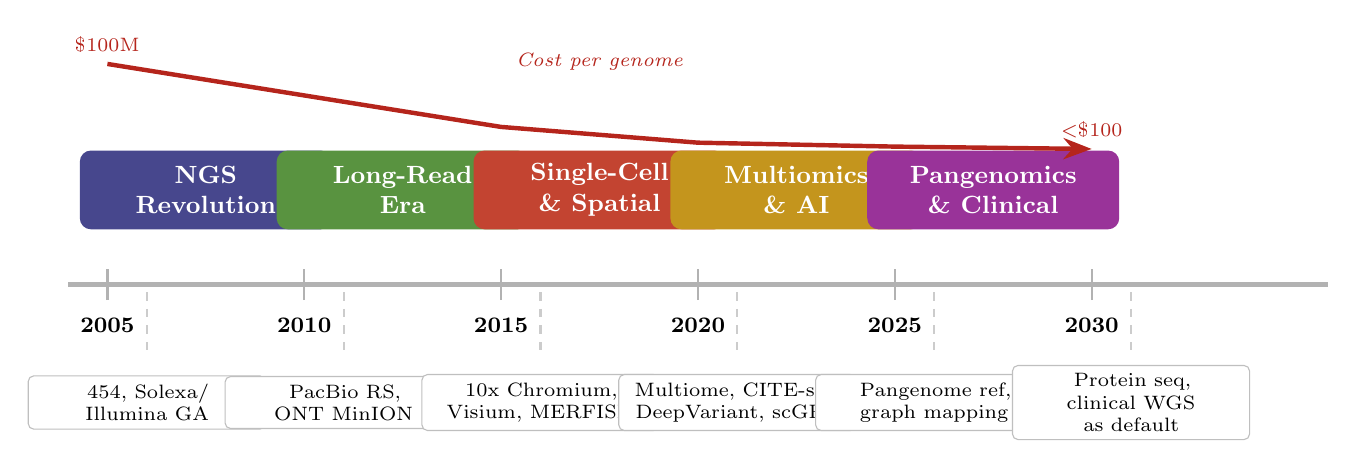
\begin{tikzpicture}[
  >=Stealth,
  era/.style={draw=none, fill=#1, rounded corners=4pt,
    minimum width=3.2cm, minimum height=1cm,
    font=\small\bfseries, text=white, align=center},
  tech/.style={draw=gray!50, fill=white, rounded corners=2pt,
    font=\scriptsize, inner sep=3pt, align=center, text width=2.8cm},
  timeline/.style={ultra thick, gray!60},
  connector/.style={thick, gray!40, dashed}
]

% Timeline
\draw[timeline] (0,0) -- (16,0);
\foreach \x/\yr in {0.5/2005, 3/2010, 5.5/2015, 8/2020, 10.5/2025, 13/2030} {
  \draw[gray!60, thick] (\x,-0.2) -- (\x,0.2);
  \node[below, font=\footnotesize\bfseries] at (\x,-0.3) {\yr};
}

% Era labels
\node[era=MidnightBlue!80] at (1.75,1.2) {NGS\\Revolution};
\node[era=OliveGreen!80] at (4.25,1.2) {Long-Read\\Era};
\node[era=BrickRed!80] at (6.75,1.2) {Single-Cell\\\& Spatial};
\node[era=Goldenrod!90!black] at (9.25,1.2) {Multiomics\\\& AI};
\node[era=violet!80] at (11.75,1.2) {Pangenomics\\\& Clinical};

% Technologies - above timeline
\node[tech] at (1,-1.5) {454, Solexa/\\Illumina GA};
\node[tech] at (3.5,-1.5) {PacBio RS,\\ONT MinION};
\node[tech] at (6,-1.5) {10x Chromium,\\Visium, MERFISH};
\node[tech] at (8.5,-1.5) {Multiome, CITE-seq,\\DeepVariant, scGPT};
\node[tech] at (11,-1.5) {Pangenome ref,\\graph mapping};
\node[tech] at (13.5,-1.5) {Protein seq,\\clinical WGS\\as default};

% Connecting lines
\foreach \x in {1, 3.5, 6, 8.5, 11, 13.5} {
  \draw[connector] (\x,-0.1) -- (\x,-0.9);
}

% Cost trajectory overlay
\draw[BrickRed, ultra thick, ->]
  (0.5,2.8) node[above, font=\scriptsize, BrickRed] {\$100M}
  -- (3,2.4) -- (5.5,2.0) -- (8,1.8) -- (10.5,1.75) -- (13,1.72)
  node[above, font=\scriptsize, BrickRed] {$<$\$100};
\node[BrickRed, font=\scriptsize\itshape, above] at (6.75,2.6) {Cost per genome};

\end{tikzpicture}
\caption[The evolving sequencing technology landscape.]{Timeline of the sequencing technology landscape, showing major eras, representative technologies, and the continuing decline in per-genome cost. Each era builds upon the previous ones; earlier technologies do not disappear but are augmented by newer capabilities.}
\label{fig:emerging:landscape}
\end{figure}


\begin{figure}[htbp]
\centering
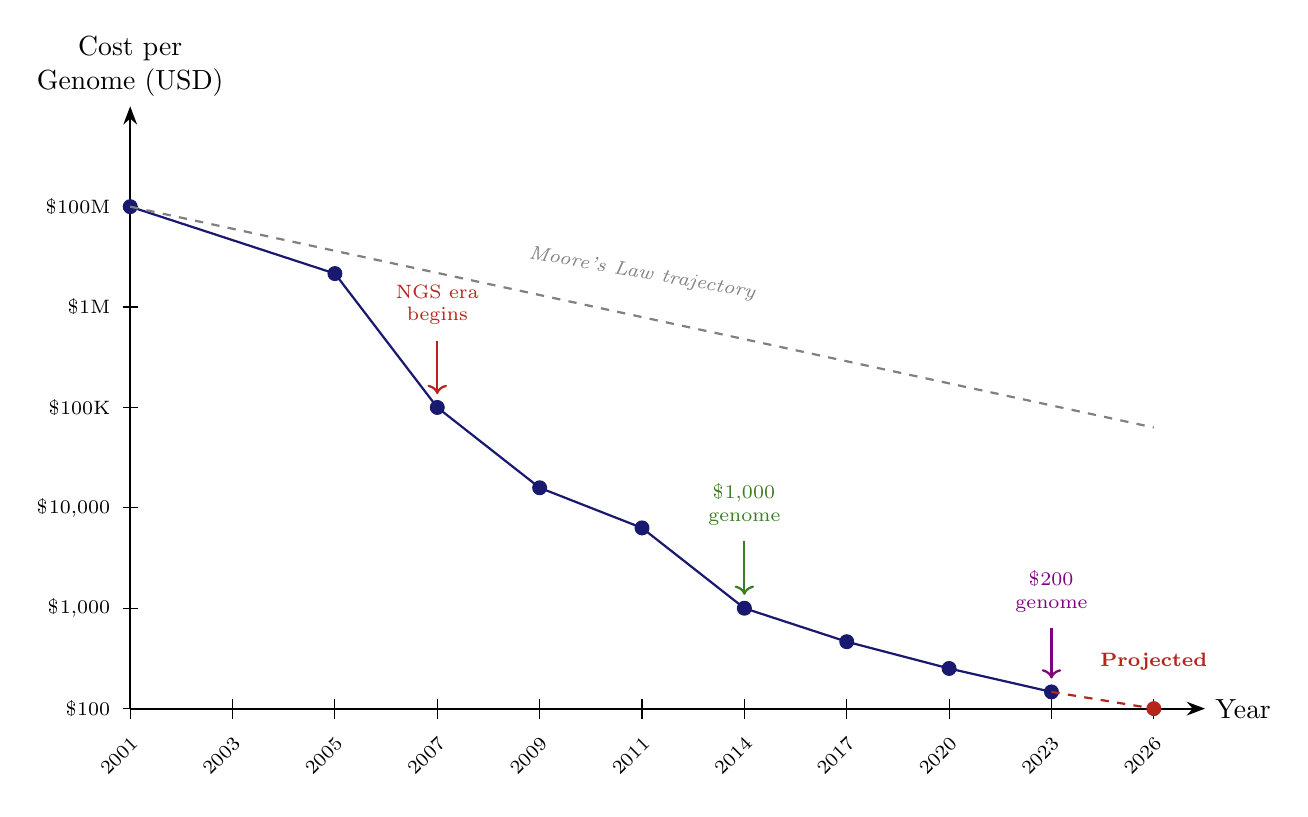
\begin{tikzpicture}[x=0.65cm, y=0.85cm]
  % Axes
  \draw[thick, -{Stealth}] (0,0) -- (21,0) node[right] {Year};
  \draw[thick, -{Stealth}] (0,0) -- (0,9) node[above, align=center] {Cost per\\Genome (USD)};

  % Y-axis labels (log scale)
  \foreach \y/\lab in {0/\$100, 1.5/\$1{,}000, 3/\$10{,}000, 4.5/\$100K, 6/\$1M, 7.5/\$100M} {
    \draw (-0.15,\y) -- (0.15,\y);
    \node[left, font=\scriptsize] at (-0.2,\y) {\lab};
  }

  % X-axis labels
  \foreach \x/\yr in {0/2001, 2/2003, 4/2005, 6/2007, 8/2009, 10/2011, 12/2014, 14/2017, 16/2020, 18/2023, 20/2026} {
    \draw (\x,-0.15) -- (\x,0.15);
    \node[below, rotate=45, anchor=north east, font=\scriptsize] at (\x,-0.2) {\yr};
  }

  % Data points
  \filldraw[MidnightBlue] (0,7.5) circle (2.5pt);    % 2001: $95M
  \filldraw[MidnightBlue] (4,6.5) circle (2.5pt);    % 2005: $30M
  \filldraw[MidnightBlue] (6,4.5) circle (2.5pt);    % 2007: $100K (NGS)
  \filldraw[MidnightBlue] (8,3.3) circle (2.5pt);    % 2009: $20K
  \filldraw[MidnightBlue] (10,2.7) circle (2.5pt);   % 2011: $7K
  \filldraw[MidnightBlue] (12,1.5) circle (2.5pt);   % 2014: $1K
  \filldraw[MidnightBlue] (14,1.0) circle (2.5pt);   % 2017: $600
  \filldraw[MidnightBlue] (16,0.6) circle (2.5pt);   % 2020: $300
  \filldraw[MidnightBlue] (18,0.25) circle (2.5pt);  % 2023: $200
  \filldraw[BrickRed] (20,0.0) circle (2.5pt);        % 2026: ~$100

  % Line
  \draw[MidnightBlue, thick]
    (0,7.5) -- (4,6.5) -- (6,4.5) -- (8,3.3) --
    (10,2.7) -- (12,1.5) -- (14,1.0) -- (16,0.6) --
    (18,0.25);
  \draw[BrickRed, thick, dashed] (18,0.25) -- (20,0.0);

  % Moore's Law reference
  \draw[gray, dashed, thick] (0,7.5) -- (20,4.2);
  \node[gray, rotate=-10, font=\scriptsize\itshape] at (10,6.5) {Moore's Law trajectory};

  % Annotations
  \draw[->, BrickRed, thick] (6,5.5) -- (6,4.7);
  \node[BrickRed, above, align=center, font=\scriptsize] at (6,5.6) {NGS era\\begins};

  \draw[->, OliveGreen, thick] (12,2.5) -- (12,1.7);
  \node[OliveGreen, above, align=center, font=\scriptsize] at (12,2.6) {\$1{,}000\\genome};

  \draw[->, violet, thick] (18,1.2) -- (18,0.45);
  \node[violet, above, align=center, font=\scriptsize] at (18,1.3) {\$200\\genome};

  \node[BrickRed, font=\scriptsize\bfseries] at (20,0.7) {Projected};

\end{tikzpicture}
\caption[Sequencing cost trajectory: 2001--2026.]{The cost of sequencing a human genome from 2001 to 2026 (projected), shown on a logarithmic scale. The precipitous drop beginning around 2007 coincides with the introduction of NGS technologies. The decline has consistently outpaced Moore's Law. The dashed segment indicates projected costs. Data based on NHGRI estimates.}
\label{fig:emerging:cost-trajectory}
\end{figure}


\section{Summary}
\label{sec:emerging:summary}

This chapter has surveyed the frontiers of sequencing technology and the broader genomics landscape. Key takeaways include:

\begin{itemize}[itemsep=3pt]
  \item \textbf{Protein sequencing} technologies (Quantum-Si, Nautilus) are bringing sequencing-like approaches to the proteome, promising integrated multi-molecular profiling.
  \item \textbf{In situ sequencing} (STARmap, ExSeq) reads sequences directly within intact tissues at subcellular resolution, merging the spatial and molecular information domains.
  \item \textbf{Synthetic long reads} and linked-read technologies (TELL-seq, stLFR) extract long-range information from short-read platforms, providing a cost-effective alternative to true long-read sequencing for some applications.
  \item \textbf{Ultra-long nanopore reads} ($>$4\megabase{}) enable assembly of the most complex genomic regions, including centromeres and large structural variants.
  \item \textbf{AI and machine learning} have transformed basecalling (Dorado, DeepConsensus), variant calling (DeepVariant), and biological interpretation (genomic language models, single-cell foundation models such as scGPT and Geneformer).
  \item \textbf{Cloud computing and GPU acceleration} (Terra, DRAGEN, Parabricks) are making large-scale genomic analysis accessible and fast, while workflow managers (Nextflow Tower/Seqera) provide the orchestration layer.
  \item \textbf{Portable sequencing} has taken genomics to the field---from Ebola outbreak zones to the International Space Station---and is enabling rapid clinical diagnosis in hours rather than days.
  \item \textbf{Pangenomics} and graph-based references (vg, minigraph) are replacing the single linear reference genome paradigm, reducing reference bias and improving accuracy for all populations.
  \item \textbf{Ethical considerations}---genetic privacy, equitable access, data sovereignty, and responsible use of genomic information---are as important as the technologies themselves and must be actively addressed by the genomics community.
\end{itemize}

The sequencing revolution that began with Sanger's dideoxy method in 1977 shows no signs of slowing. If anything, the pace of innovation is accelerating, driven by the convergence of molecular biology, engineering, and artificial intelligence. The researchers and clinicians who will shape the next decade of genomics are those who combine deep understanding of the biological questions with fluency in the rapidly evolving technological landscape described throughout this book.


% Part VII: Bioinformatics and Data Analysis
\part{Bioinformatics and Data Analysis}
\chapter{Bioinformatics Fundamentals}
\label{ch:bioinfofundamentals}

\begin{sourcebox}
The alignment and file-processing foundations are anchored by the BWA and SAMtools papers \cite{li2009bwa,li2009}. File-format authority ultimately lies in the current specification, while command behavior lies in the named software release and its help text.
\end{sourcebox}

\begin{keyconcept}
Bioinformatics is the interdisciplinary field that develops and applies computational methods to analyse, interpret, and manage biological data---particularly the vast quantities of sequence data generated by modern \acrshort{NGS} platforms. Mastering bioinformatics fundamentals is essential for any researcher who generates or analyses sequencing data: without appropriate computational tools and practices, even the highest-quality sequencing data cannot be translated into biological insight.
\end{keyconcept}

\section{What Is Bioinformatics?}
\label{sec:bioinf:what}

At its core, bioinformatics sits at the intersection of biology, computer science, mathematics, and statistics. It encompasses the development of algorithms and software tools for processing raw sequencing data (alignment, quality control, variant calling), the design of databases and ontologies for organising biological knowledge, and the application of statistical and machine-learning methods for extracting meaningful patterns from high-dimensional datasets.

For the genomics practitioner, bioinformatics is not a separate discipline but an integral part of every sequencing experiment. The moment reads leave the sequencer, the project becomes a computational endeavour. Understanding the computing environment, file formats, key tools, programming languages, and workflow management systems described in this chapter is therefore a prerequisite for every subsequent analysis chapter in this book.

%=============================================================================
\section{Computing Environment Setup}
\label{sec:bioinf:computing}
%=============================================================================

\subsection{Linux/Unix Basics for Bioinformatics}
\label{subsec:bioinf:linux}

Nearly all bioinformatics software is developed for, and best supported on, Linux and Unix-like operating systems. Even researchers who use macOS or Windows on their personal machines will typically run analyses on a Linux-based high-performance computing (HPC) cluster or cloud instance. The command-line interface (CLI) is the primary means of interaction.

Essential command-line skills include:

\begin{itemize}[itemsep=2pt]
  \item \textbf{Navigation:} \texttt{cd}, \texttt{ls}, \texttt{pwd}, \texttt{tree}.
  \item \textbf{File manipulation:} \texttt{cp}, \texttt{mv}, \texttt{rm}, \texttt{mkdir}, \texttt{ln -s} (symbolic links).
  \item \textbf{Text processing:} \texttt{cat}, \texttt{head}, \texttt{tail}, \texttt{less}, \texttt{wc}, \texttt{grep}, \texttt{sed}, \texttt{awk}, \texttt{cut}, \texttt{sort}, \texttt{uniq}.
  \item \textbf{Compression:} \texttt{gzip}/\texttt{gunzip}, \texttt{bgzip} (block-gzip for indexed access), \texttt{zcat}.
  \item \textbf{Pipes and redirection:} combining commands with \texttt{|}, \texttt{>}, \texttt{>>}, \texttt{2>}.
  \item \textbf{Process management:} \texttt{top}/\texttt{htop}, \texttt{ps}, \texttt{kill}, \texttt{nohup}, \texttt{screen}/\texttt{tmux}.
  \item \textbf{Permissions:} \texttt{chmod}, \texttt{chown}; understanding \texttt{rwx} triplets.
  \item \textbf{Environment variables:} \texttt{export}, \texttt{PATH}, \texttt{.bashrc}/\texttt{.bash\_profile}.
\end{itemize}

\begin{tipbox}[title={Screen and Tmux}]
Use \texttt{screen} or \texttt{tmux} to create persistent terminal sessions on remote servers. If your SSH connection drops during a long-running job, the process continues safely inside the session. This is indispensable for interactive bioinformatics work on HPC clusters.
\end{tipbox}

\begin{lstlisting}[language=bash,caption={Essential Linux commands for bioinformatics.},label=lst:linux-basics]
# Count reads in a FASTQ file (4 lines per read)
wc -l sample.fastq | awk '{print $1/4}'

# Extract chromosome 1 alignments from a BAM file
samtools view -b input.bam chr1 > chr1.bam

# Sort a BED file and merge overlapping intervals
sort -k1,1 -k2,2n peaks.bed | bedtools merge > merged.bed

# View the first few records of a gzipped VCF
zcat variants.vcf.gz | grep -v "^#" | head -20

# Monitor disk usage of a project directory
du -sh /data/project/*
\end{lstlisting}

\subsection{Package Managers}
\label{subsec:bioinf:packagemanagers}

Installing bioinformatics software can be challenging due to complex dependency chains. Modern package managers greatly simplify this process:

\begin{description}[style=nextline, font=\bfseries, itemsep=4pt]
  \item[Conda / Mamba]
  Conda is the most widely used package manager in bioinformatics. It manages both software binaries and their dependencies within isolated \textit{environments}, preventing version conflicts between projects. The \texttt{bioconda} channel provides over 11,000 bioinformatics packages. \texttt{Mamba} is a drop-in replacement for \texttt{conda} with significantly faster dependency resolution.

  \item[Pip]
  Python's native package manager. Used for Python-specific packages not available through Conda (e.g., niche libraries on PyPI). Best used \textit{within} a Conda environment to avoid conflicts with system Python.

  \item[Bioconductor]
  The primary repository for R-based bioinformatics packages. Bioconductor provides a curated, versioned ecosystem of packages for genomic data analysis, including \software{DESeq2}, \software{edgeR}, \software{GenomicRanges}, and hundreds of others. Packages are installed via \texttt{BiocManager::install()}.
\end{description}

\begin{lstlisting}[language=bash,caption={Setting up a Conda environment for bioinformatics.},label=lst:conda-setup]
# Install Miniforge (includes mamba)
curl -L -O https://github.com/conda-forge/miniforge/releases/latest/download/Miniforge3-Linux-x86_64.sh
bash Miniforge3-Linux-x86_64.sh

# Create an environment for an RNA-seq project
mamba create -n rnaseq -c conda-forge -c bioconda \
  fastqc=0.12.1 fastp=0.23.4 star=2.7.11b \
  subread=2.0.6 samtools=1.19 multiqc=1.21

# Activate the environment
mamba activate rnaseq

# Export the environment for reproducibility
mamba env export > environment.yml
\end{lstlisting}

\subsection{Containers: Docker and Singularity/Apptainer}
\label{subsec:bioinf:containers}

Containers provide a higher level of reproducibility than package managers by encapsulating the entire software environment---operating system libraries, tools, and configuration---into a portable, immutable image.

\begin{description}[style=nextline, font=\bfseries, itemsep=4pt]
  \item[Docker]
  The most widely used container platform. Docker images are available for virtually every bioinformatics tool (e.g., on Docker Hub or Quay.io). Docker requires root privileges to run, which limits its use on shared HPC clusters.

  \item[Singularity / Apptainer]
  Designed for HPC environments where users do not have root access. Singularity (now rebranded as Apptainer) can run Docker images directly without modification. Most HPC centres support Singularity/Apptainer.
\end{description}

\begin{lstlisting}[language=bash,caption={Using containers for bioinformatics.},label=lst:containers]
# Pull and run a Docker image for FastQC
docker pull biocontainers/fastqc:v0.12.1
docker run --rm -v $(pwd):/data biocontainers/fastqc:v0.12.1 \
  fastqc /data/sample_R1.fastq.gz /data/sample_R2.fastq.gz

# On HPC: convert Docker image to Singularity/Apptainer
singularity pull docker://biocontainers/fastqc:v0.12.1
singularity exec fastqc_v0.12.1.sif fastqc sample_R1.fastq.gz

# BioContainers provides images for most bioinformatics tools
# See: https://biocontainers.pro
\end{lstlisting}

\begin{keyconcept}[title={Containers for Reproducibility}]
A Conda environment specifies what software to install; a container specifies the exact binary files, libraries, and operating system state. Containers provide ``bit-for-bit'' reproducibility---the same container will produce identical results on any machine, even years later. For published analyses, containers are the gold standard for computational reproducibility.
\end{keyconcept}

\subsection{HPC Clusters: SLURM, PBS/Torque, SGE}
\label{subsec:bioinf:hpc}

Most bioinformatics analyses require computational resources beyond what a laptop or desktop can provide. High-performance computing (HPC) clusters provide shared pools of CPUs, RAM, and storage. Jobs are submitted through a \textbf{workload manager} (also called a job scheduler):

\begin{description}[style=nextline, font=\bfseries, itemsep=3pt]
  \item[SLURM (Simple Linux Utility for Resource Management)]
  The most widely deployed scheduler in academic HPC. Jobs are submitted with \texttt{sbatch}, monitored with \texttt{squeue}, and cancelled with \texttt{scancel}.

  \item[PBS/Torque]
  An older but still common scheduler. Jobs are submitted with \texttt{qsub} and monitored with \texttt{qstat}.

  \item[SGE (Sun Grid Engine) / Open Grid Scheduler]
  Legacy scheduler found in some older installations. Also uses \texttt{qsub}/\texttt{qstat} syntax.
\end{description}

\begin{lstlisting}[language=bash,caption={SLURM job submission for a bioinformatics task.},label=lst:slurm]
#!/bin/bash
#SBATCH --job-name=bwa_align
#SBATCH --output=logs/bwa_%j.out
#SBATCH --error=logs/bwa_%j.err
#SBATCH --cpus-per-task=16
#SBATCH --mem=32G
#SBATCH --time=06:00:00
#SBATCH --partition=standard

# Load modules or activate environment
source activate wgs_pipeline

# Run BWA-MEM2 alignment
bwa-mem2 mem -t 16 \
  /ref/GRCh38.fa \
  sample_R1.fastq.gz sample_R2.fastq.gz \
  | samtools sort -@ 4 -o sample.sorted.bam -

samtools index sample.sorted.bam
\end{lstlisting}

\subsection{Cloud Computing for Genomics}
\label{subsec:bioinf:cloud}

Cloud computing offers elastic, on-demand computational resources without the capital investment of purchasing hardware. The three major cloud providers each offer genomics-specific services:

\begin{itemize}[itemsep=3pt]
  \item \textbf{Amazon Web Services (AWS):} AWS HealthOmics for managed genomics workflows; S3 for storage; EC2 for compute; AWS Batch for job scheduling. The Registry of Open Data on AWS hosts public genomics datasets (1000 Genomes, TCGA, gnomAD).
  \item \textbf{Google Cloud Platform (GCP):} Google Cloud Life Sciences API; BigQuery for large-scale variant analysis; Terra platform (Broad Institute) for WDL-based workflows running on GCP.
  \item \textbf{Microsoft Azure:} Azure Genomics; Cromwell on Azure for WDL workflows; integration with Microsoft's healthcare data solutions.
\end{itemize}

\begin{warningbox}[title={Cloud Cost Management}]
Cloud computing can become expensive if not carefully managed. A single misconfigured pipeline can generate thousands of dollars in compute charges within hours. Always set budget alerts, use spot/preemptible instances for fault-tolerant workloads (50--80\% cost savings), and shut down instances when not in use. Estimate costs before running large analyses using the provider's pricing calculators.
\end{warningbox}

%=============================================================================
\section{Bioinformatics File Formats}
\label{sec:bioinf:formats}
%=============================================================================

A thorough understanding of file formats is essential for working with sequencing data. Each format serves a specific purpose in the analysis pipeline, and knowing their structure helps in debugging problems and writing custom analyses.

\subsection{FASTA: Reference Sequences}
\label{subsec:bioinf:fasta}

The FASTA format is one of the simplest and oldest bioinformatics formats, used to store nucleotide or protein sequences. Each record consists of a header line beginning with \texttt{>} followed by one or more lines of sequence:

\begin{lstlisting}[caption={FASTA format example.},label=lst:fasta]
>chr1 Homo sapiens chromosome 1
NNNNNNNNNNNNNNNNNNNNNNNNNNNNNNNNNNNNNNNNNNNNNNNNNN
NNNNNNNNNNNNNNNNNNNNNNNNNNNNNNGATAATCTACTACTACTCAG
TGGCCAACACCTGATCCTGACAGCTGGAGTAAGGAACCTGAAGTCCCTA
AAACTCATCAATGTTCTTTAGAGACTTACCAGGACCACTTCGTGAGGGA
>chr2 Homo sapiens chromosome 2
NNNNNNNNNNNNNNNNNNNNNNNNNNNNNNNNNNNNNNNNNNNNNNNNNN
AGAGATCAGCTCAGGAGAGTCTCTTGAAGAAATCTGATTCACTGTATGG
\end{lstlisting}

Reference genomes (e.g., GRCh38/hg38 for human) are distributed in FASTA format. For efficient random access, FASTA files are indexed with \texttt{samtools faidx}, producing a \texttt{.fai} index file. Many tools also require a sequence dictionary (\texttt{.dict}) created with \software{Picard} or \software{samtools}.

\subsection{FASTQ: Raw Sequencing Reads}
\label{subsec:bioinf:fastq}

FASTQ is the universal output format for sequencing instruments. Each read consists of exactly four lines:

\begin{lstlisting}[caption={FASTQ format example with Phred quality encoding.},label=lst:fastq]
@NB501234:45:H3YTNBGX3:1:11101:24563:1038 1:N:0:ACGTACGT
NTGCAAGCAGTTCAGGATCAGTCGAGACTTCAATGTCGATCTACGTAGC
+
#AAFFJJJJJJJJJJJJJJJJJJJJJJJJJJJJJJJJJJJJJJJJJJ
\end{lstlisting}

\begin{description}[style=nextline, font=\bfseries, itemsep=2pt]
  \item[Line 1 (@)] Read identifier containing instrument name, run ID, flow cell coordinates, and index sequence. Paired reads share the same ID but differ in the \texttt{1:} or \texttt{2:} field.
  \item[Line 2] The nucleotide sequence (A, C, G, T, N).
  \item[Line 3 (+)] A separator line (sometimes repeats the read ID, but usually just \texttt{+}).
  \item[Line 4] ASCII-encoded quality scores, one character per base. Each character encodes a \textbf{Phred quality score}: $Q = -10 \log_{10}(P_{\text{error}})$.
\end{description}

\begin{keyconcept}[title={Phred Quality Scores}]
Phred scores encode the probability of a base call being incorrect:

\begin{center}
\begin{tabular}{ccc}
\toprule
\textbf{Phred Score} & \textbf{Error Probability} & \textbf{Accuracy} \\
\midrule
10 & 1 in 10 & 90\% \\
20 & 1 in 100 & 99\% \\
30 & 1 in 1,000 & 99.9\% \\
40 & 1 in 10,000 & 99.99\% \\
\bottomrule
\end{tabular}
\end{center}

Modern Illumina instruments use the \textbf{Phred+33} encoding: the ASCII character code minus 33 gives the quality score. For example, the character \texttt{J} has ASCII code 74, so $Q = 74 - 33 = 41$. The character \texttt{\#} has ASCII code 35, so $Q = 35 - 33 = 2$ (very low quality).
\end{keyconcept}

FASTQ files are almost always gzip-compressed (\texttt{.fastq.gz}) because raw data is enormous---a single 30$\times$ human genome generates approximately 90~Gb of compressed FASTQ data.

\subsection{SAM/BAM/CRAM: Alignment Files}
\label{subsec:bioinf:sambam}

The Sequence Alignment/Map (SAM) format and its binary counterpart BAM store read alignments against a reference genome. CRAM is a more compressed alternative that uses reference-based compression.

Each alignment record contains the following key fields:

\begin{longtable}{l p{10cm}}
\caption{Key fields in SAM/BAM alignment records.} \label{tab:sam-fields} \\
\toprule
\textbf{Field} & \textbf{Description} \\
\midrule
\endfirsthead
\toprule
\textbf{Field} & \textbf{Description} \\
\midrule
\endhead
\texttt{QNAME} & Read name (query name). Identical for both reads of a pair. \\
\texttt{FLAG} & Bitwise flag encoding read properties: paired, properly paired, unmapped, mate unmapped, reverse strand, first/second in pair, duplicate, supplementary, secondary. \\
\texttt{RNAME} & Reference sequence name (chromosome) to which the read is aligned. \\
\texttt{POS} & 1-based leftmost mapping position on the reference. \\
\texttt{MAPQ} & Mapping quality score (Phred-scaled probability that the mapping position is wrong). MAPQ~0 means the read maps equally well to multiple locations. \\
\texttt{CIGAR} & Compact string describing the alignment: \texttt{M} (match/mismatch), \texttt{I} (insertion to reference), \texttt{D} (deletion from reference), \texttt{S} (soft clipping), \texttt{H} (hard clipping), \texttt{N} (skipped region, e.g., intron in RNA-seq). Example: \texttt{76M2I50M3S} means 76 matched bases, 2-bp insertion, 50 matched bases, 3 soft-clipped bases. \\
\texttt{RNEXT} & Reference name of the mate's alignment (for paired-end reads). \\
\texttt{PNEXT} & Position of the mate's alignment. \\
\texttt{TLEN} & Observed template length (insert size). \\
\texttt{SEQ} & Read sequence. \\
\texttt{QUAL} & Base quality string (same encoding as FASTQ). \\
\bottomrule
\end{longtable}

\begin{lstlisting}[caption={SAM format example (two paired-end reads).},label=lst:sam]
@HD VN:1.6  SO:coordinate
@SQ SN:chr1 LN:248956422
@RG ID:sample1 SM:sample1 PL:ILLUMINA
read001  99  chr1  10050  60  151M  =  10250  351  ACGTACGT...  JJJJJJJJ...
read001  147 chr1  10250  60  151M  =  10050  -351 TGCATGCA...  JJJJJJJJ...
\end{lstlisting}

\begin{warningbox}[title={SAM FLAG Field}]
The FLAG field is a bitwise integer that encodes multiple properties simultaneously. Use \texttt{samtools flags} to decode a FLAG value, or the SAM flag decoder at \texttt{https://broadinstitute.github.io/picard/explain-flags.html}. Common FLAG values: 99 (paired, properly paired, mate on reverse strand, first in pair), 147 (paired, properly paired, read on reverse strand, second in pair), 4 (unmapped).
\end{warningbox}

BAM files are always sorted (by coordinate or by name) and indexed (\texttt{.bai} or \texttt{.csi} index) for efficient random access. CRAM achieves 30--60\% smaller file sizes than BAM by storing only the differences from the reference.

\subsection{BED: Genomic Intervals}
\label{subsec:bioinf:bed}

BED (Browser Extensible Data) format represents genomic intervals with a simple tab-delimited structure. Coordinates are \textbf{0-based, half-open}: the start position is 0-based and inclusive, the end position is exclusive.

\begin{lstlisting}[caption={BED format variants (BED3, BED6, BED12).},label=lst:bed]
# BED3: chromosome, start, end
chr1  1000  2000
chr1  3000  4500

# BED6: adds name, score, strand
chr1  1000  2000  peak1  500  +
chr1  3000  4500  peak2  300  -

# BED12: adds thickStart, thickEnd, itemRgb, blockCount,
#         blockSizes, blockStarts (used for transcript models)
chr1  11873  14409  NR_046018  0  +  11873  11873  0  3  354,109,1189,  0,739,1347,
\end{lstlisting}

\begin{warningbox}[title={Coordinate Systems}]
BED uses 0-based, half-open coordinates. SAM/BAM and VCF use 1-based, fully closed coordinates. GFF/GTF uses 1-based, fully closed coordinates. The position ``chr1:1000--2000'' in BED corresponds to ``chr1:1001--2000'' in SAM. Coordinate system mismatches are one of the most common sources of off-by-one errors in bioinformatics.
\end{warningbox}

\subsection{GFF/GTF: Gene Annotations}
\label{subsec:bioinf:gff}

GFF3 (General Feature Format version 3) and GTF (Gene Transfer Format, essentially GFF2) store gene and transcript annotations. These files define the locations of genes, transcripts, exons, coding sequences, and other genomic features.

\begin{lstlisting}[caption={GTF format example (GENCODE).},label=lst:gtf]
chr1  HAVANA  gene        11869  14409  .  +  .  gene_id "ENSG00000223972"; gene_name "DDX11L1";
chr1  HAVANA  transcript  11869  14409  .  +  .  gene_id "ENSG00000223972"; transcript_id "ENST00000456328";
chr1  HAVANA  exon        11869  12227  .  +  .  gene_id "ENSG00000223972"; transcript_id "ENST00000456328";
chr1  HAVANA  exon        12613  12721  .  +  .  gene_id "ENSG00000223972"; transcript_id "ENST00000456328";
chr1  HAVANA  exon        13221  14409  .  +  .  gene_id "ENSG00000223972"; transcript_id "ENST00000456328";
\end{lstlisting}

GENCODE annotations (the standard for human and mouse) are available in both GTF and GFF3 formats. Most RNA-seq quantification tools (STAR, featureCounts, Salmon) accept GTF.

\subsection{VCF/BCF: Variant Calls}
\label{subsec:bioinf:vcf}

The Variant Call Format (VCF) stores genetic variants (SNPs, indels, structural variants). BCF is the binary, indexed version. The VCF format is critical for genomics and clinical sequencing:

\begin{lstlisting}[caption={VCF format example with key fields.},label=lst:vcf]
##fileformat=VCFv4.3
##INFO=<ID=DP,Number=1,Type=Integer,Description="Total Depth">
##INFO=<ID=AF,Number=A,Type=Float,Description="Allele Frequency">
##FORMAT=<ID=GT,Number=1,Type=String,Description="Genotype">
##FORMAT=<ID=DP,Number=1,Type=Integer,Description="Read Depth">
##FORMAT=<ID=GQ,Number=1,Type=Integer,Description="Genotype Quality">
#CHROM  POS     ID        REF  ALT  QUAL  FILTER  INFO          FORMAT     SAMPLE1
chr1    12345   rs123456  A    G    99    PASS    DP=50;AF=0.5  GT:DP:GQ   0/1:50:99
chr1    67890   .         CT   C    85    PASS    DP=40;AF=0.3  GT:DP:GQ   0/1:40:85
\end{lstlisting}

Key VCF concepts:
\begin{itemize}[itemsep=2pt]
  \item \textbf{INFO field:} site-level annotations (total depth, allele frequency, functional impact).
  \item \textbf{FORMAT field:} defines per-sample fields that follow.
  \item \textbf{Genotype (GT):} \texttt{0/0} = homozygous reference, \texttt{0/1} = heterozygous, \texttt{1/1} = homozygous alternate, \texttt{./.} = missing.
  \item \textbf{FILTER:} \texttt{PASS} if the variant passes all quality filters; otherwise a semicolon-separated list of filter names.
\end{itemize}

\subsection{BigWig and BedGraph: Coverage Tracks}
\label{subsec:bioinf:bigwig}

BigWig and BedGraph files represent continuous signal tracks across the genome, such as read coverage depth or ChIP-seq signal intensity. BedGraph is a text format; BigWig is a compressed, indexed binary format suitable for genome browser visualization. BigWig files are created from BAM files using tools like \software{deepTools} \texttt{bamCoverage} or \texttt{bedtools genomecov}.

\subsection{HDF5 and AnnData (h5ad): Single-Cell Data}
\label{subsec:bioinf:h5ad}

Single-cell datasets are stored in HDF5-based formats. The \texttt{.h5ad} format (AnnData) is the standard for the Scanpy ecosystem in Python, storing the expression matrix, cell metadata, gene metadata, dimensionality reductions, and graphs in a single file. The Seurat ecosystem in R uses \texttt{.rds} (serialized R objects) or the newer \texttt{.h5Seurat} format. Loom (\texttt{.loom}) is another HDF5-based format used by some tools.

\subsection{Hi-C Contact Matrices: Pairs, Cool, and .hic}
\label{subsec:bioinf:hic}

Hi-C data (3D genome organization) uses specialized formats:
\begin{itemize}[itemsep=2pt]
  \item \textbf{.pairs:} Text format listing pairs of interacting genomic loci, defined by the 4DN consortium.
  \item \textbf{.cool / .mcool:} HDF5-based format for contact matrices at one or multiple resolutions, used by the \software{cooler} library.
  \item \textbf{.hic:} Binary format used by \software{Juicer} and \software{JuiceBox} for contact matrix storage and visualization.
\end{itemize}

\subsection{10x Genomics MEX Format}
\label{subsec:bioinf:10x}

The Market Exchange (MEX) format from Cell Ranger consists of three files stored together in a directory:
\begin{itemize}[itemsep=2pt]
  \item \texttt{matrix.mtx.gz}: Sparse matrix in Matrix Market format (rows = genes, columns = barcodes).
  \item \texttt{barcodes.tsv.gz}: Cell barcodes (one per line).
  \item \texttt{features.tsv.gz}: Gene/feature identifiers and names.
\end{itemize}
This format is read by \software{Scanpy} (\texttt{sc.read\_10x\_mtx()}), \software{Seurat} (\texttt{Read10X()}), and other single-cell tools.

%=============================================================================
\section{Key Bioinformatics Tools}
\label{sec:bioinf:tools}
%=============================================================================

\subsection{samtools: The Swiss Army Knife of BAM Files}
\label{subsec:bioinf:samtools}

\software{samtools} is the most fundamental bioinformatics tool, providing operations on SAM/BAM/CRAM files:

\begin{lstlisting}[language=bash,caption={Essential samtools commands.},label=lst:samtools]
# View BAM header
samtools view -H sample.bam

# Convert SAM to sorted BAM
samtools sort -@ 8 -o sample.sorted.bam sample.sam

# Index a sorted BAM file
samtools index sample.sorted.bam

# View alignments in a region
samtools view sample.sorted.bam chr1:1000000-2000000

# Filter: keep only properly paired, uniquely mapped reads (MAPQ >= 30)
samtools view -b -f 2 -q 30 sample.sorted.bam > filtered.bam

# Generate alignment statistics
samtools flagstat sample.sorted.bam
samtools idxstats sample.sorted.bam
samtools stats sample.sorted.bam > sample.stats.txt

# Calculate per-base depth
samtools depth -a sample.sorted.bam > depth.txt

# Merge multiple BAM files
samtools merge merged.bam sample1.bam sample2.bam sample3.bam
\end{lstlisting}

\subsection{bedtools: Interval Arithmetic}
\label{subsec:bioinf:bedtools}

\software{bedtools} provides a comprehensive suite of operations for manipulating genomic intervals:

\begin{lstlisting}[language=bash,caption={Common bedtools operations.},label=lst:bedtools]
# Intersect peaks with gene promoters
bedtools intersect -a peaks.bed -b promoters.bed -wa -wb > overlap.bed

# Find peaks that do NOT overlap with blacklist regions
bedtools intersect -a peaks.bed -b blacklist.bed -v > clean_peaks.bed

# Merge overlapping intervals
bedtools merge -i sorted_peaks.bed -d 100 > merged.bed

# Find closest gene to each peak
bedtools closest -a peaks.bed -b genes.bed -d > closest.bed

# Compute genome-wide coverage from a BAM file
bedtools genomecov -ibam sample.bam -bg > coverage.bedgraph

# Generate windows across the genome
bedtools makewindows -g genome.sizes -w 10000 > windows.bed

# Compute Jaccard similarity between two sets of intervals
bedtools jaccard -a set1.bed -b set2.bed
\end{lstlisting}

\subsection{Picard: Duplicate Marking and Metrics}
\label{subsec:bioinf:picard}

\software{Picard} (Broad Institute) provides utilities for BAM manipulation, with \texttt{MarkDuplicates} being the most commonly used:

\begin{lstlisting}[language=bash,caption={Picard MarkDuplicates and metrics collection.},label=lst:picard]
# Mark PCR duplicates
java -jar picard.jar MarkDuplicates \
  I=sample.sorted.bam \
  O=sample.dedup.bam \
  M=sample.dup_metrics.txt \
  REMOVE_DUPLICATES=false

# Collect alignment summary metrics
java -jar picard.jar CollectAlignmentSummaryMetrics \
  R=reference.fa I=sample.dedup.bam O=alignment_metrics.txt

# Collect insert size distribution
java -jar picard.jar CollectInsertSizeMetrics \
  I=sample.dedup.bam O=insert_metrics.txt H=insert_hist.pdf
\end{lstlisting}

\subsection{IGV: Visual Inspection}
\label{subsec:bioinf:igv}

The Integrative Genomics Viewer (IGV) is an essential desktop application for visually inspecting alignments, variants, and other genomic features. Load BAM files, VCF files, BED files, and BigWig tracks to examine specific loci. Visual inspection is critical for validating computational results---many false-positive variant calls or artefacts become obvious upon manual review in IGV.

\begin{tipbox}[title={Always Inspect Key Results in IGV}]
Before reporting important findings---a novel variant, an unexpected peak, a suspicious fusion event---take five minutes to look at the raw data in IGV. Computational tools can make systematic errors that are immediately obvious to a human viewer. Journals and reviewers increasingly expect IGV screenshots for key findings.
\end{tipbox}

\subsection{deepTools: Coverage and Visualization}
\label{subsec:bioinf:deeptools}

\software{deepTools} provides powerful commands for computing and visualizing coverage from BAM files:

\begin{lstlisting}[language=bash,caption={deepTools for coverage analysis and visualization.},label=lst:deeptools]
# Generate normalized coverage track (RPKM)
bamCoverage -b sample.bam -o sample.bw \
  --normalizeUsing RPKM --binSize 10 -p 8

# Compute correlation between replicates
multiBamSummary bins -b rep1.bam rep2.bam rep3.bam \
  -o results.npz -p 8
plotCorrelation -in results.npz --corMethod spearman \
  -o correlation_heatmap.pdf --plotFileFormat pdf

# Generate heatmap of signal around TSS
computeMatrix reference-point -S chip.bw input.bw \
  -R genes.bed -a 3000 -b 3000 -o matrix.gz
plotHeatmap -m matrix.gz -o heatmap.pdf
\end{lstlisting}

\subsection{MultiQC: Aggregating QC Reports}
\label{subsec:bioinf:multiqc}

\software{MultiQC} scans a project directory for output files from dozens of bioinformatics tools (FastQC, STAR, samtools, Picard, featureCounts, etc.) and compiles them into a single interactive HTML report. This is invaluable for identifying outlier samples and systematic quality issues across a cohort:

\begin{lstlisting}[language=bash,caption={Running MultiQC to aggregate quality reports.},label=lst:multiqc]
# Run MultiQC on an entire project directory
multiqc /project/results/ -o /project/multiqc_report/

# Run with specific module selection and title
multiqc . --module fastqc --module star --module picard \
  --title "RNA-seq QC Report" -o qc_report/
\end{lstlisting}

%=============================================================================
\section{Algorithms and Data Structures for Sequence Analysis}
\label{sec:bioinf:algorithms}
%=============================================================================

Understanding the algorithmic foundations of sequence alignment and search is essential for choosing the right tool for a given problem and for interpreting performance characteristics. This section covers the key data structures and algorithms that underpin modern read aligners and sequence analysis tools.

\subsection{Suffix Arrays}
\label{subsec:bioinf:suffixarrays}

\begin{keyconcept}[title={Suffix Array}]
A \textbf{suffix array} (SA) of a string $T$ of length $n$ is an array of integers that specifies the lexicographic ordering of all $n$ suffixes of $T$. Formally, $\text{SA}[i] = j$ means that the $j$-th suffix (i.e., $T[j..n]$) is the $i$-th smallest suffix in lexicographic order.
\end{keyconcept}

Given a reference genome $T$ of length $n$, the suffix array enables exact string matching in $O(m \log n)$ time for a pattern of length $m$, using binary search over the sorted suffixes. More advanced techniques reduce this to $O(m + \log n)$ using the longest common prefix (LCP) array.

Suffix arrays can be constructed in $O(n \log n)$ time using the prefix-doubling algorithm, or in $O(n)$ time using the SA-IS (Suffix Array by Induced Sorting) algorithm. In practice, the SA-IS algorithm is preferred for genome-scale strings:

\begin{equation}
\text{SA construction: } O(n) \text{ time, } O(n) \text{ space (SA-IS algorithm)}
\end{equation}

Suffix arrays are closely related to the Burrows-Wheeler Transform: given the suffix array, the BWT can be computed in $O(n)$ time, and vice versa. This relationship is exploited by read aligners such as \software{BWA} and \software{Bowtie2}.

\subsection{Burrows-Wheeler Transform and FM-Index}
\label{subsec:bioinf:bwt}

\begin{keyconcept}[title={Burrows-Wheeler Transform}]
The \textbf{Burrows-Wheeler Transform} (BWT) of a string $T$ is constructed by:
\begin{enumerate}[nosep]
  \item Appending a sentinel character \texttt{\$} (lexicographically smaller than all others) to $T$.
  \item Generating all cyclic rotations of the string.
  \item Sorting these rotations lexicographically.
  \item Taking the \textbf{last column} of the sorted rotation matrix.
\end{enumerate}
The resulting string $\text{BWT}(T)$ is a permutation of $T$ that is highly compressible because characters from similar sequence contexts are grouped together.
\end{keyconcept}

The BWT has a remarkable property called the \textbf{LF mapping} (Last-to-First mapping): the $i$-th occurrence of character $c$ in the last column corresponds to the $i$-th occurrence of $c$ in the first column. Since the first column is simply the sorted characters of $T$, it can be represented implicitly. The LF mapping enables navigation through the original string without storing it explicitly.

The \textbf{FM-index} (Full-text Minute-space index) combines the BWT with auxiliary data structures---the \textbf{C array} (cumulative character counts) and the \textbf{Occ table} (occurrence counts of each character up to each position in the BWT)---to support exact pattern matching in $O(m)$ time, where $m$ is the pattern length:

\begin{align}
\text{Backward search step: } & \text{top} = C[c] + \text{Occ}(c, \text{top} - 1) + 1 \\
                               & \text{bot} = C[c] + \text{Occ}(c, \text{bot})
\end{align}

Starting from the last character of the query pattern and proceeding backwards, each step narrows the suffix array interval $[\text{top}, \text{bot})$ to those suffixes that match an increasingly longer suffix of the pattern. When $\text{top} \geq \text{bot}$, the pattern does not occur in $T$; otherwise, the number of occurrences is $\text{bot} - \text{top}$.

\begin{tipbox}[title={Why BWA-MEM Uses the FM-Index}]
\software{BWA-MEM} and \software{BWA-MEM2} use the FM-index to find exact matches (seeds) between the read and the reference genome in $O(m)$ time per seed, independent of genome size. The FM-index of the human genome ($\sim$3~\gigabase) requires approximately 3--5~GB of RAM, making it practical for commodity hardware. Without the FM-index, naive string searching would require $O(nm)$ time per read, which is infeasible for billions of reads against a multi-gigabase genome.
\end{tipbox}

\subsection{Smith-Waterman vs Seed-and-Extend}
\label{subsec:bioinf:alignment}

\subsubsection{Smith-Waterman Local Alignment}

The \textbf{Smith-Waterman} (SW) algorithm finds the optimal local alignment between two sequences using dynamic programming. Given a query of length $m$ and a reference of length $n$, the recurrence is:

\begin{equation}
H(i,j) = \max \begin{cases}
  0 \\
  H(i-1, j-1) + s(a_i, b_j) \\
  H(i-1, j) - d \\
  H(i, j-1) - d
\end{cases}
\end{equation}

where $s(a_i, b_j)$ is the substitution score (positive for match, negative for mismatch) and $d$ is the gap penalty. The algorithm runs in $O(mn)$ time and $O(mn)$ space (reducible to $O(m)$ space with traceback modifications).

For aligning a single 150\basepair{} read against the 3~\gigabase{} human genome, Smith-Waterman would require $\sim 150 \times 3 \times 10^9 = 4.5 \times 10^{11}$ operations per read---clearly impractical for millions of reads. Even with SIMD-accelerated implementations, full Smith-Waterman against a whole genome is too slow for routine alignment.

\subsubsection{Seed-and-Extend Strategy}

The \textbf{seed-and-extend} paradigm makes alignment tractable for whole genomes:

\begin{enumerate}[itemsep=2pt]
  \item \textbf{Seeding:} Find exact $k$-mer matches (seeds) between the read and the reference using an index (FM-index, hash table, or minimizer index). Seeds are short exact matches that identify candidate alignment locations.
  \item \textbf{Chaining:} Group co-linear seeds that are consistent with a single alignment (same strand, approximately correct distance apart). This step identifies the most promising candidate regions.
  \item \textbf{Extension:} Perform banded Smith-Waterman (or similar DP) alignment only in a narrow band around the chained seeds. Banded alignment restricts the DP matrix to a diagonal band of width $w$, reducing time complexity to $O(mw)$ where $w \ll n$.
\end{enumerate}

\begin{description}[style=nextline, font=\bfseries, itemsep=3pt]
  \item[BWA-MEM2]
  Uses FM-index-based seeding with super-maximal exact matches (SMEMs), followed by Smith-Waterman extension with affine gap penalties. \software{BWA-MEM2} additionally uses AVX-512 SIMD instructions for 2--3$\times$ speedup over the original \software{BWA-MEM}.

  \item[minimap2]
  Uses a minimizer-based index (rather than an FM-index) for seeding, followed by chaining with a gap-cost-aware dynamic programming algorithm, and base-level alignment with the KSW2 library. \software{minimap2} supports both short reads and long reads (PacBio, Oxford Nanopore) by adjusting seeding and chaining parameters.
\end{description}

\subsection{Algorithm Complexity Reference}
\label{subsec:bioinf:complexity}

\begin{table}[htbp]
\centering
\caption{Time and space complexity of key sequence analysis algorithms.}
\label{tab:algorithm-complexity}
\small
\renewcommand{\arraystretch}{1.3}
\begin{tabularx}{\textwidth}{@{}l l l X@{}}
\toprule
\textbf{Algorithm} & \textbf{Time} & \textbf{Space} & \textbf{Used By} \\
\midrule
BWT construction (SA-IS) & $O(n)$ & $O(n)$ & BWA, Bowtie2 (index build) \\
\addlinespace
FM-index query & $O(m)$ per pattern & $O(n)$ & BWA-MEM, BWA-MEM2, Bowtie2 \\
\addlinespace
Suffix array (binary search) & $O(m \log n)$ per query & $O(n)$ & Suffix array-based tools \\
\addlinespace
Smith-Waterman (full DP) & $O(mn)$ & $O(mn)$ & SSW library, Parasail, BLAST \\
\addlinespace
Banded Smith-Waterman & $O(mw)$ & $O(mw)$ & BWA-MEM2, minimap2 (extension) \\
\addlinespace
Seed-and-extend (overall) & $O(m + \text{hits} \cdot w)$ & $O(n)$ index & BWA-MEM2, minimap2, STAR \\
\addlinespace
Minimizer index construction & $O(n)$ & $O(n/w)$ & minimap2, Kraken2, Strobealign \\
\addlinespace
minimap2 chaining & $O(N \log N)$ & $O(N)$ & minimap2 ($N$ = seed count) \\
\addlinespace
De Bruijn graph construction & $O(n)$ & $O(|\Sigma|^k)$ worst & SPAdes, Velvet, Trinity (assembly) \\
\bottomrule
\end{tabularx}
\end{table}

\begin{warningbox}[title={Practical vs Theoretical Complexity}]
Asymptotic complexity does not capture the full performance picture. SIMD vectorisation (used by BWA-MEM2 and minimap2) can accelerate Smith-Waterman alignment by 10--50$\times$. Cache locality, I/O bandwidth, and memory access patterns often dominate real-world runtime. For example, \software{minimap2} uses minimizers to reduce the index size by $\sim w$-fold compared to a full suffix array, making it faster in practice despite similar asymptotic complexity. Always benchmark tools on representative data rather than relying solely on complexity analysis.
\end{warningbox}

%=============================================================================
\section{Programming Languages for Bioinformatics}
\label{sec:bioinf:programming}
%=============================================================================

\subsection{Python for Bioinformatics}
\label{subsec:bioinf:python}

Python has become the dominant general-purpose programming language in bioinformatics, valued for its readability, extensive libraries, and strong community support.

\begin{description}[style=nextline, font=\bfseries, itemsep=3pt]
  \item[Biopython] Reading/writing FASTA/FASTQ, BLAST parsing, sequence manipulation.
  \item[pysam] Python wrapper for htslib; reading/writing SAM/BAM/VCF files programmatically.
  \item[Scanpy] The standard framework for single-cell RNA-seq analysis (preprocessing, clustering, visualization).
  \item[pandas] Tabular data manipulation (metadata tables, count matrices).
  \item[NumPy / SciPy] Numerical computing, statistical tests.
  \item[matplotlib / seaborn] Publication-quality plotting.
  \item[pyGenomeTracks] Visualization of genomic tracks (BigWig, BED, Hi-C).
\end{description}

\begin{lstlisting}[language=Python,caption={Python example: reading a BAM file with pysam.},label=lst:pysam]
import pysam

# Open BAM file and count reads per chromosome
bamfile = pysam.AlignmentFile("sample.sorted.bam", "rb")
for chrom in bamfile.references:
    count = bamfile.count(contig=chrom)
    print(f"{chrom}: {count} reads")

# Extract reads with MAPQ >= 30 from a specific region
high_qual = [read for read in bamfile.fetch("chr1", 1000000, 2000000)
             if read.mapping_quality >= 30 and not read.is_duplicate]
print(f"High-quality reads in region: {len(high_qual)}")
bamfile.close()
\end{lstlisting}

\subsection{R for Bioinformatics}
\label{subsec:bioinf:r}

R, through the Bioconductor ecosystem, remains the language of choice for statistical genomics and many specialized analysis workflows:

\begin{description}[style=nextline, font=\bfseries, itemsep=3pt]
  \item[DESeq2 / edgeR / limma-voom] Differential gene expression analysis from RNA-seq count data.
  \item[GenomicRanges / GenomicAlignments] Efficient representation and manipulation of genomic intervals in R.
  \item[Seurat] Single-cell RNA-seq analysis (alternative to Scanpy).
  \item[ggplot2] The grammar of graphics---the gold standard for publication-quality statistical graphics.
  \item[clusterProfiler] Gene ontology and pathway enrichment analysis.
  \item[DiffBind] Differential binding analysis for ChIP-seq and ATAC-seq.
\end{description}

\begin{lstlisting}[language=R,caption={R example: basic DESeq2 differential expression analysis.},label=lst:deseq2-example]
library(DESeq2)

# Load count matrix and sample metadata
counts <- read.csv("counts.csv", row.names = 1)
coldata <- read.csv("sample_info.csv", row.names = 1)

# Create DESeq2 dataset
dds <- DESeqDataSetFromMatrix(countData = counts,
                               colData = coldata,
                               design = ~ condition)

# Run differential expression analysis
dds <- DESeq(dds)
res <- results(dds, contrast = c("condition", "treated", "control"))

# Filter significant genes (adjusted p-value < 0.05, |log2FC| > 1)
sig <- subset(res, padj < 0.05 & abs(log2FoldChange) > 1)
cat("Significant DE genes:", nrow(sig), "\n")
\end{lstlisting}

\subsection{When to Use Which Language}
\label{subsec:bioinf:whichlang}

\begin{table}[htbp]
\centering
\caption{Choosing between Python and R for bioinformatics tasks.}
\label{tab:python-vs-r}
\small
\begin{tabularx}{\textwidth}{l X X}
\toprule
\textbf{Task} & \textbf{Python} & \textbf{R (Bioconductor)} \\
\midrule
Single-cell RNA-seq & Scanpy (dominant) & Seurat (dominant) \\
Differential expression & pyDESeq2 (newer) & DESeq2, edgeR (gold standard) \\
Genomic interval operations & pybedtools, pysam & GenomicRanges \\
Statistical modeling & statsmodels, scipy & Built-in, extensive \\
Machine learning & scikit-learn, PyTorch & caret, mlr3 \\
Workflow scripting & Excellent & Less common \\
Plotting & matplotlib, seaborn & ggplot2 (gold standard) \\
Pipeline integration & Snakemake (Python-native) & Both via CLI calls \\
\bottomrule
\end{tabularx}
\end{table}

\begin{tipbox}[title={Use Both Languages}]
Most bioinformatics projects benefit from using both Python and R. A common pattern: use Python (with Snakemake or Nextflow) for the upstream pipeline (alignment, counting, QC), then switch to R for the downstream statistical analysis (differential expression, enrichment) and publication-quality figures. The \texttt{reticulate} package in R and \texttt{rpy2} in Python allow cross-language communication when needed.
\end{tipbox}

%=============================================================================
\section{Workflow Management Systems}
\label{sec:bioinf:workflows}
%=============================================================================

\subsection{Why Workflow Managers?}
\label{subsec:bioinf:whywfm}

A typical bioinformatics analysis involves dozens of sequential and parallel processing steps, each with specific software, parameters, input files, and output files. Running these steps manually is error-prone, difficult to reproduce, and impossible to scale. Workflow management systems address these challenges by providing:

\begin{itemize}[itemsep=2pt]
  \item \textbf{Reproducibility:} The workflow definition is a complete, executable record of the analysis.
  \item \textbf{Scalability:} Automatic parallelization across samples, with support for HPC clusters and cloud.
  \item \textbf{Portability:} Workflows can run on laptops, clusters, or cloud with minimal modification.
  \item \textbf{Resumability:} If a step fails, the workflow resumes from where it left off after the issue is fixed.
  \item \textbf{Provenance tracking:} Automatic logging of which inputs, software versions, and parameters produced each output.
\end{itemize}

\subsection{Snakemake}
\label{subsec:bioinf:snakemake}

\subsubsection{Philosophy and Core Concepts}

Snakemake is a Python-based workflow engine that uses a declarative, file-centric approach inspired by GNU Make. The central abstraction is the \textbf{rule}, which defines how to create output files from input files:

\begin{itemize}[itemsep=2pt]
  \item \textbf{Rules:} Each rule specifies \texttt{input}, \texttt{output}, and a \texttt{shell} command (or \texttt{run} block for Python code).
  \item \textbf{Wildcards:} Placeholders (e.g., \texttt{\{sample\}}) that are automatically resolved, enabling rules to apply to any sample.
  \item \textbf{\texttt{expand()}:} Function that generates file lists by combining wildcards with sample lists.
  \item \textbf{Directed Acyclic Graph (DAG):} Snakemake infers the dependency graph from input/output relationships and executes steps in the correct order.
  \item \textbf{Conda integration:} Each rule can specify a Conda environment YAML file, ensuring tool versions are pinned per step.
  \item \textbf{Container support:} Rules can use Singularity/Apptainer containers for maximum reproducibility.
  \item \textbf{Cluster execution:} Native support for SLURM, PBS, SGE, and cloud (AWS, GCP) via profiles.
\end{itemize}

\subsubsection{Complete Snakemake QC Pipeline Example}

\begin{lstlisting}[language=Python,caption={Complete Snakemake workflow for a basic FASTQ QC pipeline.},label=lst:snakemake-qc]
# Snakefile for basic QC pipeline
configfile: "config.yaml"

SAMPLES = config["samples"]

rule all:
    input:
        expand("results/fastqc/{sample}_{read}_fastqc.html",
               sample=SAMPLES, read=["R1", "R2"]),
        expand("results/fastp/{sample}_R1.trimmed.fastq.gz",
               sample=SAMPLES),
        "results/multiqc/multiqc_report.html"

rule fastqc_raw:
    input:
        "data/{sample}_{read}.fastq.gz"
    output:
        html="results/fastqc/{sample}_{read}_fastqc.html",
        zip="results/fastqc/{sample}_{read}_fastqc.zip"
    threads: 2
    conda:
        "envs/qc.yaml"
    shell:
        "fastqc -t {threads} -o results/fastqc/ {input}"

rule fastp_trim:
    input:
        r1="data/{sample}_R1.fastq.gz",
        r2="data/{sample}_R2.fastq.gz"
    output:
        r1="results/fastp/{sample}_R1.trimmed.fastq.gz",
        r2="results/fastp/{sample}_R2.trimmed.fastq.gz",
        html="results/fastp/{sample}_fastp.html",
        json="results/fastp/{sample}_fastp.json"
    threads: 4
    conda:
        "envs/qc.yaml"
    params:
        qual=config.get("min_quality", 20),
        len=config.get("min_length", 50)
    shell:
        """
        fastp -i {input.r1} -I {input.r2} \
          -o {output.r1} -O {output.r2} \
          -h {output.html} -j {output.json} \
          --qualified_quality_phred {params.qual} \
          --length_required {params.len} \
          --detect_adapter_for_pe \
          --thread {threads}
        """

rule multiqc:
    input:
        expand("results/fastqc/{sample}_{read}_fastqc.zip",
               sample=SAMPLES, read=["R1", "R2"]),
        expand("results/fastp/{sample}_fastp.json",
               sample=SAMPLES)
    output:
        "results/multiqc/multiqc_report.html"
    conda:
        "envs/qc.yaml"
    shell:
        "multiqc results/ -o results/multiqc/ --force"
\end{lstlisting}

\begin{lstlisting}[caption={config.yaml for the Snakemake QC pipeline.},label=lst:snakemake-config]
# config.yaml
samples:
  - sample1
  - sample2
  - sample3

min_quality: 20
min_length: 50
\end{lstlisting}

\begin{lstlisting}[caption={Conda environment file for QC tools (envs/qc.yaml).},label=lst:conda-qc]
# envs/qc.yaml
name: qc
channels:
  - conda-forge
  - bioconda
dependencies:
  - fastqc=0.12.1
  - fastp=0.23.4
  - multiqc=1.21
\end{lstlisting}

\begin{lstlisting}[language=bash,caption={Running the Snakemake QC pipeline.},label=lst:snakemake-run]
# Dry run (show what would be executed)
snakemake -n --cores 8

# Execute locally with 8 cores
snakemake --cores 8 --use-conda

# Execute on a SLURM cluster
snakemake --cores 100 --use-conda --slurm \
  --default-resources slurm_partition=standard mem_mb=8000

# Generate the workflow DAG visualization
snakemake --dag | dot -Tpdf > dag.pdf
\end{lstlisting}

\subsection{Nextflow}
\label{subsec:bioinf:nextflow}

\subsubsection{Philosophy and Core Concepts}

Nextflow uses a \textbf{dataflow programming model} where data flows through a network of processes connected by \textbf{channels}. It is written in Groovy (a JVM language) and uses DSL2 syntax for modular workflow design:

\begin{itemize}[itemsep=2pt]
  \item \textbf{Processes:} Independent computational steps, each with defined inputs, outputs, and a script.
  \item \textbf{Channels:} Asynchronous queues that connect process inputs to outputs. Data items flow through channels one at a time, enabling automatic parallelism.
  \item \textbf{Channel operators:} \texttt{map}, \texttt{filter}, \texttt{collect}, \texttt{combine}, \texttt{groupTuple}, \texttt{flatten}---powerful transformations for routing and reshaping data.
  \item \textbf{DSL2 modules:} Processes can be defined in separate module files and imported, promoting reuse.
  \item \textbf{Profiles:} Named configuration sets (e.g., \texttt{-profile docker}, \texttt{-profile slurm}) that switch between execution environments.
  \item \textbf{nf-core:} A community of curated, production-ready Nextflow pipelines (over 100 pipelines for genomics, transcriptomics, epigenomics, metagenomics, and more).
  \item \textbf{Seqera Platform (Nextflow Tower):} A web-based monitoring and management platform for Nextflow pipelines.
\end{itemize}

\subsubsection{Complete Nextflow QC Pipeline Example}

\begin{lstlisting}[language=Java,caption={Complete Nextflow DSL2 workflow for a basic FASTQ QC pipeline (main.nf).},label=lst:nextflow-qc]
#!/usr/bin/env nextflow
nextflow.enable.dsl = 2

// Parameters
params.reads    = "data/*_{R1,R2}.fastq.gz"
params.outdir   = "results"
params.min_qual = 20
params.min_len  = 50

log.info """
  ===================================
  Q C   P I P E L I N E
  ===================================
  reads   : ${params.reads}
  outdir  : ${params.outdir}
  min_qual: ${params.min_qual}
  min_len : ${params.min_len}
  ===================================
""".stripIndent()

process FASTQC {
    tag "${sample_id}"
    publishDir "${params.outdir}/fastqc", mode: 'copy'
    conda 'bioconda::fastqc=0.12.1'
    cpus 2

    input:
    tuple val(sample_id), path(reads)

    output:
    path("*.html"), emit: html
    path("*.zip"),  emit: zip

    script:
    """
    fastqc -t ${task.cpus} ${reads}
    """
}

process FASTP {
    tag "${sample_id}"
    publishDir "${params.outdir}/fastp", mode: 'copy'
    conda 'bioconda::fastp=0.23.4'
    cpus 4

    input:
    tuple val(sample_id), path(reads)

    output:
    tuple val(sample_id), path("*_trimmed.fastq.gz"), emit: trimmed
    path("*.html"), emit: html
    path("*.json"), emit: json

    script:
    def (r1, r2) = reads
    """
    fastp -i ${r1} -I ${r2} \
      -o ${sample_id}_R1_trimmed.fastq.gz \
      -O ${sample_id}_R2_trimmed.fastq.gz \
      -h ${sample_id}_fastp.html \
      -j ${sample_id}_fastp.json \
      --qualified_quality_phred ${params.min_qual} \
      --length_required ${params.min_len} \
      --detect_adapter_for_pe \
      --thread ${task.cpus}
    """
}

process MULTIQC {
    publishDir "${params.outdir}/multiqc", mode: 'copy'
    conda 'bioconda::multiqc=1.21'

    input:
    path('*')

    output:
    path("multiqc_report.html")

    script:
    """
    multiqc . -o . --force
    """
}

workflow {
    read_pairs_ch = Channel
        .fromFilePairs(params.reads, checkIfExists: true)

    FASTQC(read_pairs_ch)
    FASTP(read_pairs_ch)

    ch_multiqc = FASTQC.out.zip
        .mix(FASTP.out.json)
        .collect()

    MULTIQC(ch_multiqc)
}
\end{lstlisting}

\begin{lstlisting}[caption={nextflow.config for the QC pipeline.},label=lst:nextflow-config]
// nextflow.config
profiles {
    standard {
        process.executor = 'local'
        process.cpus = 4
        process.memory = '8 GB'
    }
    slurm {
        process.executor = 'slurm'
        process.queue = 'standard'
        process.cpus = 4
        process.memory = '8 GB'
        process.time = '2h'
    }
    docker {
        docker.enabled = true
    }
    singularity {
        singularity.enabled = true
        singularity.autoMounts = true
    }
}

process {
    errorStrategy = 'retry'
    maxRetries = 2
}
\end{lstlisting}

\begin{lstlisting}[language=bash,caption={Running the Nextflow QC pipeline.},label=lst:nextflow-run]
# Run locally
nextflow run main.nf --reads "data/*_{R1,R2}.fastq.gz"

# Run with SLURM profile
nextflow run main.nf -profile slurm

# Run with Docker containers
nextflow run main.nf -profile docker

# Resume a failed/interrupted run
nextflow run main.nf -resume

# Run an nf-core pipeline directly
nextflow run nf-core/rnaseq -r 3.14.0 \
  --input samplesheet.csv --genome GRCh38 -profile singularity
\end{lstlisting}

\subsection{Snakemake vs Nextflow: Detailed Comparison}
\label{subsec:bioinf:smk-vs-nf}

\begin{table}[htbp]
\centering
\caption{Comprehensive comparison of Snakemake and Nextflow workflow management systems.}
\label{tab:smk-vs-nf}
\small
\renewcommand{\arraystretch}{1.3}
\begin{tabularx}{\textwidth}{@{}l X X@{}}
\toprule
\textbf{Feature} & \textbf{Snakemake} & \textbf{Nextflow} \\
\midrule
Language & Python-based & Groovy-based (JVM) \\
Paradigm & Declarative, file-centric (Make-like) & Dataflow, channel-based \\
Dependency resolution & From file I/O relationships & From channel connections \\
Learning curve & Lower (Python knowledge helps) & Steeper (new channel/operator concepts) \\
Wildcard system & Powerful, built-in wildcards & Channels and tuple patterns \\
Modularity & Include/module rules, wrappers & DSL2 modules, sub-workflows \\
Conda integration & Per-rule \texttt{conda:} directive & Per-process \texttt{conda} directive \\
Container support & Singularity, Docker & Docker, Singularity, Podman \\
Cloud support & AWS, GCP (via profiles) & AWS, GCP, Azure (native executors) \\
HPC support & SLURM, PBS, SGE (profiles) & SLURM, PBS, SGE, LSF, etc. \\
Community pipelines & Snakemake Workflow Catalog & nf-core (100+ curated pipelines) \\
Monitoring & Panoptes (limited) & Seqera Platform / Nextflow Tower \\
Caching/resume & Based on file timestamps/checksums & Based on task hash (robust) \\
Reporting & Built-in HTML report & Nextflow reports, Tower dashboard \\
Popularity & Strong in academia (Europe) & Strong in industry and nf-core community \\
\bottomrule
\end{tabularx}
\end{table}

\begin{tipbox}[title={Choosing a Workflow Manager}]
Both Snakemake and Nextflow are excellent choices. If your group uses Python extensively and values the Make-like file-centric model, Snakemake may feel more natural. If you prefer dataflow programming, need robust cloud integration, or want to leverage the extensive nf-core pipeline library, Nextflow is an excellent choice. Many bioinformatics groups successfully use both, selecting the tool that best fits each project.
\end{tipbox}

\subsection{WDL (Workflow Description Language)}
\label{subsec:bioinf:wdl}

WDL is a workflow language developed by the Broad Institute, primarily used with the Cromwell execution engine and the Terra platform (a cloud-based genomics platform running on Google Cloud). GATK best-practices pipelines are officially maintained as WDL workflows. WDL uses a task-and-workflow structure similar to Nextflow's process-and-workflow model. While less widely adopted in academia than Snakemake or Nextflow, WDL is prominent in clinical genomics and large-scale variant calling projects.

\subsection{nf-core: Community-Curated Pipelines}
\label{subsec:bioinf:nfcore}

The nf-core community maintains a library of over 100 production-ready Nextflow pipelines, each following strict quality standards:

\begin{itemize}[itemsep=2pt]
  \item Standardised input formats (samplesheets)
  \item Comprehensive documentation
  \item Continuous integration testing
  \item Container support (Docker, Singularity)
  \item Built-in MultiQC reporting
  \item Reference genome handling via iGenomes or custom references
\end{itemize}

Key nf-core pipelines include: \software{nf-core/rnaseq} (RNA-seq), \software{nf-core/sarek} (WGS/WES variant calling), \software{nf-core/atacseq} (ATAC-seq), \software{nf-core/chipseq} (ChIP-seq), \software{nf-core/methylseq} (bisulfite sequencing), \software{nf-core/ampliseq} (16S amplicon), \software{nf-core/scrnaseq} (single-cell RNA-seq), and \software{nf-core/hicar} (Hi-C analysis).

%=============================================================================
\section{Version Control with Git}
\label{sec:bioinf:git}
%=============================================================================

Version control is essential for managing bioinformatics code, workflow definitions, configuration files, and analysis scripts. Git, combined with hosting platforms like GitHub or GitLab, provides:

\begin{itemize}[itemsep=2pt]
  \item \textbf{History tracking:} Every change to your analysis code is recorded with a message, author, and timestamp.
  \item \textbf{Branching:} Experiment with alternative analysis approaches without affecting the main codebase.
  \item \textbf{Collaboration:} Multiple analysts can work on the same project simultaneously.
  \item \textbf{Reproducibility:} Tag specific commits that correspond to published analyses.
\end{itemize}

\begin{lstlisting}[language=bash,caption={Essential Git workflow for a bioinformatics project.},label=lst:git]
# Initialize a repository
git init my_ngs_project && cd my_ngs_project

# Create a .gitignore for bioinformatics
cat > .gitignore << 'EOF'
# Data files (too large for Git)
*.fastq.gz
*.bam
*.bam.bai
*.vcf.gz
*.bigwig
*.h5ad

# Results (regenerated by pipeline)
results/

# Environment files
.snakemake/
work/
.nextflow*
EOF

# Stage and commit workflow files
git add Snakefile config.yaml envs/ scripts/
git commit -m "Add initial QC pipeline"

# Tag a version corresponding to a publication
git tag -a v1.0 -m "Version used in Smith et al. 2026"
git push origin main --tags
\end{lstlisting}

\begin{warningbox}[title={Never Commit Large Data Files}]
Git is designed for text files (code, configuration, documentation). Never commit large binary files (FASTQ, BAM, VCF, BigWig) to a Git repository. Use Git LFS (Large File Storage) for moderate-sized files, or track data locations in a separate manifest. Raw sequencing data should be archived in public repositories (SRA/ENA) or institutional storage systems.
\end{warningbox}

%=============================================================================
\section{Reproducibility Best Practices}
\label{sec:bioinf:reproducibility}
%=============================================================================

Reproducibility---the ability for another researcher (or your future self) to obtain the same results from the same data using the same methods---is a cornerstone of scientific integrity. In bioinformatics, achieving reproducibility requires attention to several layers:

\begin{protocolbox}[title={Reproducibility Checklist}]
\begin{enumerate}[itemsep=3pt]
  \item \textbf{Pin software versions:} Record exact versions of every tool used (e.g., via Conda environment files or container digests).
  \item \textbf{Pin reference data:} Record the exact genome build, annotation version, and database versions used (e.g., GENCODE v44, dbSNP b156).
  \item \textbf{Use a workflow manager:} Encode your entire analysis in a Snakemake or Nextflow pipeline.
  \item \textbf{Use containers:} Provide Docker/Singularity images for each step.
  \item \textbf{Use version control:} Track all code and configuration in Git.
  \item \textbf{Document parameters:} Record all command-line parameters and configuration choices, with justification.
  \item \textbf{Deposit data:} Submit raw data to SRA/ENA and processed data to GEO or equivalent repositories.
  \item \textbf{Archive code:} Deposit code on Zenodo (for DOI assignment) in addition to GitHub.
  \item \textbf{Use literate programming:} Combine analysis code, results, and narrative in R Markdown or Jupyter notebooks for downstream statistical analyses.
  \item \textbf{Set random seeds:} When using stochastic methods (e.g., UMAP, t-SNE, bootstrapping), set and record the random seed.
\end{enumerate}
\end{protocolbox}

%=============================================================================
\section{A Typical Bioinformatics Computing Stack}
\label{sec:bioinf:stack}
%=============================================================================

\Cref{fig:bioinfo-stack} illustrates the layers of a modern bioinformatics computing stack, from hardware infrastructure at the base to biological interpretation at the top.

\begin{figure}[htbp]
\centering
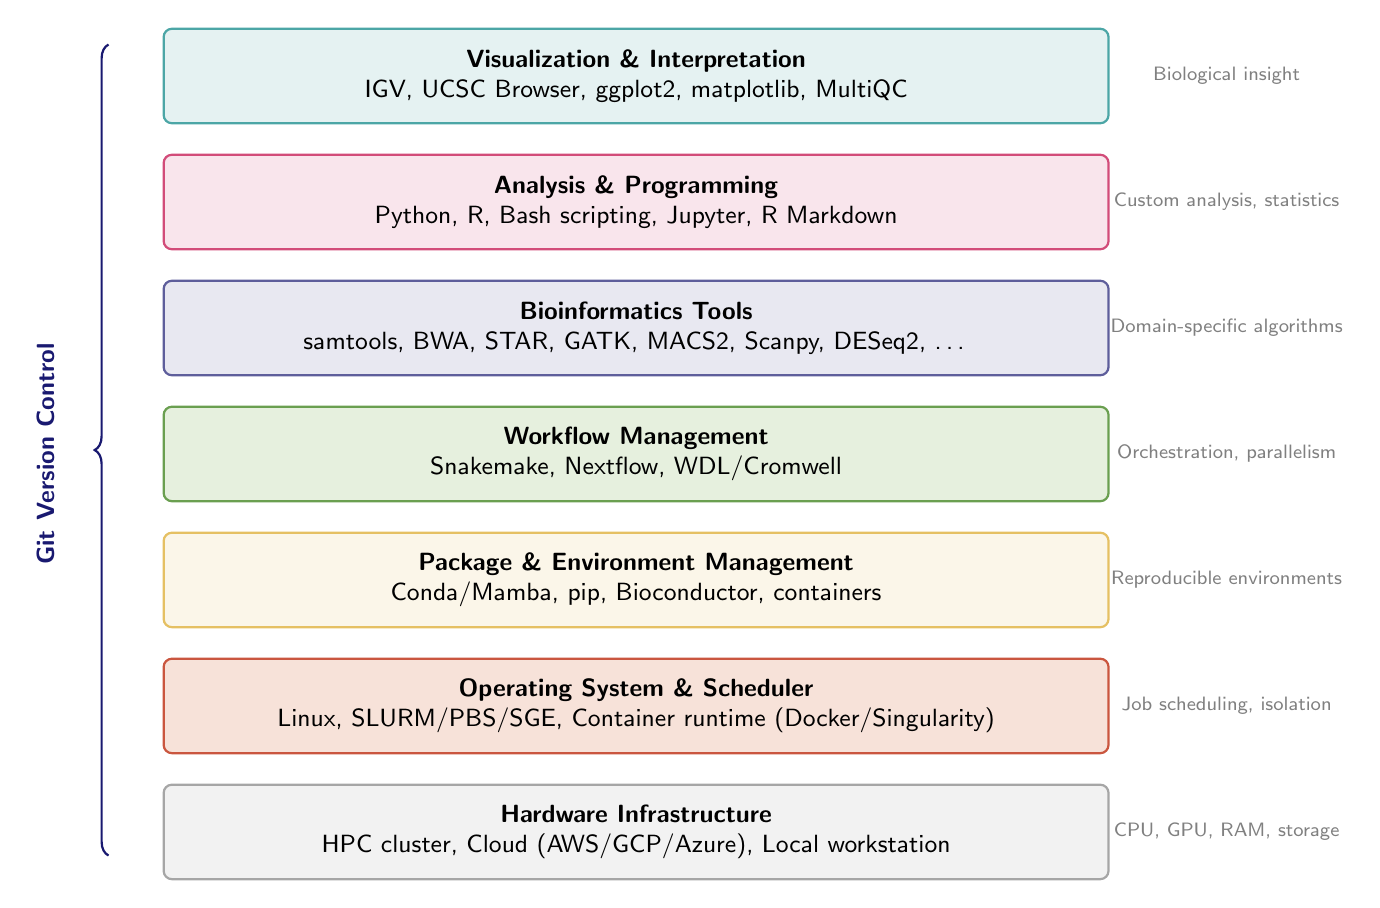
\begin{tikzpicture}[
  layer/.style={
    draw=#1!70, fill=#1!10, rounded corners=3pt,
    minimum width=12cm, minimum height=1.2cm,
    font=\sffamily\small, align=center, thick
  },
  note/.style={font=\scriptsize\sffamily, text=gray, align=left},
  arr/.style={-{Stealth[length=2.5mm]}, thick, gray!60}
]

% Stack layers from bottom to top
\node[layer=gray]        (hw)   at (0,0)    {\textbf{Hardware Infrastructure}\\HPC cluster, Cloud (AWS/GCP/Azure), Local workstation};
\node[layer=BrickRed]    (os)   at (0,1.6)  {\textbf{Operating System \& Scheduler}\\Linux, SLURM/PBS/SGE, Container runtime (Docker/Singularity)};
\node[layer=Goldenrod]   (pkg)  at (0,3.2)  {\textbf{Package \& Environment Management}\\Conda/Mamba, pip, Bioconductor, containers};
\node[layer=OliveGreen]  (wf)   at (0,4.8)  {\textbf{Workflow Management}\\Snakemake, Nextflow, WDL/Cromwell};
\node[layer=MidnightBlue](tool) at (0,6.4)  {\textbf{Bioinformatics Tools}\\samtools, BWA, STAR, GATK, MACS2, Scanpy, DESeq2, \ldots};
\node[layer=purple]      (lang) at (0,8.0)  {\textbf{Analysis \& Programming}\\Python, R, Bash scripting, Jupyter, R~Markdown};
\node[layer=teal]        (viz)  at (0,9.6)  {\textbf{Visualization \& Interpretation}\\IGV, UCSC Browser, ggplot2, matplotlib, MultiQC};

% Vertical labels on the right
\node[note] at (7.5, 0)   {CPU, GPU, RAM, storage};
\node[note] at (7.5, 1.6) {Job scheduling, isolation};
\node[note] at (7.5, 3.2) {Reproducible environments};
\node[note] at (7.5, 4.8) {Orchestration, parallelism};
\node[note] at (7.5, 6.4) {Domain-specific algorithms};
\node[note] at (7.5, 8.0) {Custom analysis, statistics};
\node[note] at (7.5, 9.6) {Biological insight};

% Side label: Version control spans all
\draw[decorate, decoration={brace, amplitude=5pt}, thick, MidnightBlue]
  (-6.7, -0.3) -- (-6.7, 10.0);
\node[rotate=90, font=\sffamily\small\bfseries, MidnightBlue] at (-7.5, 4.8) {Git Version Control};

\end{tikzpicture}
\caption[Bioinformatics computing stack.]{The layers of a modern bioinformatics computing stack. Version control (Git) spans all layers. Reproducibility requires attention at every level---from pinning software versions (environment management) to using workflow managers and containers.}
\label{fig:bioinfo-stack}
\end{figure}

%=============================================================================
\section{Summary}
\label{sec:bioinf:summary}
%=============================================================================

This chapter has introduced the foundational elements of bioinformatics that underpin all subsequent analysis chapters:

\begin{itemize}[itemsep=2pt]
  \item \textbf{Computing environment:} Linux command-line skills, package managers (Conda/Mamba), containers (Docker/Singularity), HPC clusters (SLURM), and cloud computing form the infrastructure layer.
  \item \textbf{File formats:} FASTA, FASTQ, SAM/BAM/CRAM, BED, GFF/GTF, VCF/BCF, BigWig, h5ad, and specialized formats for Hi-C and single-cell data are the lingua franca of bioinformatics.
  \item \textbf{Core tools:} samtools, bedtools, Picard, IGV, deepTools, and MultiQC are used in virtually every analysis pipeline.
  \item \textbf{Programming languages:} Python (with Biopython, pysam, Scanpy) and R (with Bioconductor, DESeq2, ggplot2) are complementary and both essential.
  \item \textbf{Workflow management:} Snakemake and Nextflow provide reproducibility, scalability, and portability for complex analysis pipelines. The nf-core community provides production-ready Nextflow pipelines.
  \item \textbf{Reproducibility:} Version control (Git), software version pinning, containers, workflow managers, and proper documentation are all essential for reproducible bioinformatics.
\end{itemize}

With these fundamentals in place, the next chapter presents complete, runnable analysis workflows for the major sequencing applications covered in this book.

\chapter{Complete Analysis Workflows}
\label{ch:workflows}

\begin{keyconcept}
This chapter provides complete, practical workflow implementations for the major \acrshort{NGS} applications covered in this book. For each application, we present both a \textbf{Snakemake} and a \textbf{Nextflow} implementation, explain every processing step, discuss key parameter choices, and highlight common pitfalls. These workflows are designed to serve as starting points that you can adapt to your specific data and research questions.
\end{keyconcept}

Each workflow follows the same structure: (1) a brief overview of the analysis logic, (2) a step-by-step explanation of what each tool does and why, (3) a complete Snakemake implementation, (4) a complete Nextflow DSL2 implementation, (5) expected outputs, and (6) common pitfalls and tips.

%=============================================================================
\section{WGS Variant Calling Pipeline}
\label{sec:wf:wgs}
%=============================================================================

\subsection{Pipeline Overview}

Whole-genome sequencing variant calling identifies single nucleotide variants (SNVs), insertions/deletions (indels), and potentially structural variants from short-read sequencing data. The GATK Best Practices pipeline is the most widely used approach for germline variant calling:

\begin{enumerate}[itemsep=2pt]
  \item \textbf{FastQC:} Raw read quality assessment.
  \item \textbf{fastp:} Adapter trimming and quality filtering.
  \item \textbf{BWA-MEM2:} Alignment to the reference genome (faster successor to BWA-MEM).
  \item \textbf{samtools sort:} Coordinate-sort the alignments.
  \item \textbf{sambamba markdup:} Mark PCR duplicates (faster alternative to Picard MarkDuplicates).
  \item \textbf{GATK HaplotypeCaller:} Per-sample variant calling in GVCF mode.
  \item \textbf{GATK GenotypeGVCFs:} Joint genotyping across samples.
  \item \textbf{GATK VQSR:} Variant Quality Score Recalibration for filtering.
  \item \textbf{VEP:} Variant Effect Predictor for functional annotation.
\end{enumerate}

\begin{tipbox}[title={Why GVCF Mode?}]
GATK HaplotypeCaller in GVCF mode (\texttt{-ERC GVCF}) produces a genomic VCF that records confidence at every position, not just variant sites. This enables efficient joint genotyping: new samples can be added to a cohort without re-calling all existing samples. For single-sample analyses, you can skip GVCF mode and call variants directly.
\end{tipbox}

\subsection{Complete Snakemake WGS Workflow}

\begin{lstlisting}[language=Python,caption={Snakemake WGS variant calling pipeline (Snakefile).},label=lst:smk-wgs]
# Snakefile -- WGS Germline Variant Calling (GATK Best Practices)
configfile: "config.yaml"

SAMPLES = config["samples"]
REF     = config["reference"]
KNOWN   = config["known_sites"]  # dbSNP, Mills, 1000G

rule all:
    input:
        "results/annotation/all_samples.annotated.vcf",
        "results/multiqc/multiqc_report.html"

rule fastp_trim:
    input:
        r1="data/{sample}_R1.fastq.gz",
        r2="data/{sample}_R2.fastq.gz"
    output:
        r1="results/trimmed/{sample}_R1.trimmed.fastq.gz",
        r2="results/trimmed/{sample}_R2.trimmed.fastq.gz",
        json="results/trimmed/{sample}_fastp.json",
        html="results/trimmed/{sample}_fastp.html"
    threads: 4
    conda: "envs/qc.yaml"
    shell:
        """
        fastp -i {input.r1} -I {input.r2} \
          -o {output.r1} -O {output.r2} \
          -j {output.json} -h {output.html} \
          --detect_adapter_for_pe --thread {threads}
        """

rule bwa_mem2_align:
    input:
        r1="results/trimmed/{sample}_R1.trimmed.fastq.gz",
        r2="results/trimmed/{sample}_R2.trimmed.fastq.gz",
        ref=REF
    output:
        bam="results/aligned/{sample}.sorted.bam"
    threads: 16
    params:
        rg=lambda wc: f"@RG\\tID:{wc.sample}\\tSM:{wc.sample}\\tPL:ILLUMINA"
    conda: "envs/align.yaml"
    shell:
        """
        bwa-mem2 mem -t {threads} -R '{params.rg}' {input.ref} \
          {input.r1} {input.r2} \
          | samtools sort -@ 4 -o {output.bam} -
        samtools index {output.bam}
        """

rule mark_duplicates:
    input:
        "results/aligned/{sample}.sorted.bam"
    output:
        bam="results/dedup/{sample}.dedup.bam",
        metrics="results/dedup/{sample}.dup_metrics.txt"
    threads: 8
    conda: "envs/align.yaml"
    shell:
        """
        sambamba markdup -t {threads} \
          {input} {output.bam} 2> {output.metrics}
        """

rule haplotype_caller:
    input:
        bam="results/dedup/{sample}.dedup.bam",
        ref=REF
    output:
        gvcf="results/gvcf/{sample}.g.vcf.gz"
    threads: 4
    conda: "envs/gatk.yaml"
    shell:
        """
        gatk HaplotypeCaller \
          -R {input.ref} -I {input.bam} \
          -O {output.gvcf} -ERC GVCF \
          --native-pair-hmm-threads {threads}
        """

rule combine_gvcfs:
    input:
        gvcfs=expand("results/gvcf/{sample}.g.vcf.gz",
                      sample=SAMPLES),
        ref=REF
    output:
        "results/genotyped/combined.g.vcf.gz"
    params:
        gvcf_args=lambda wc, input: " ".join(
            [f"-V {g}" for g in input.gvcfs])
    conda: "envs/gatk.yaml"
    shell:
        """
        gatk CombineGVCFs -R {input.ref} {params.gvcf_args} \
          -O {output}
        """

rule genotype_gvcfs:
    input:
        gvcf="results/genotyped/combined.g.vcf.gz",
        ref=REF
    output:
        "results/genotyped/all_samples.vcf.gz"
    conda: "envs/gatk.yaml"
    shell:
        """
        gatk GenotypeGVCFs -R {input.ref} -V {input.gvcf} \
          -O {output}
        """

rule vqsr_snps:
    input:
        vcf="results/genotyped/all_samples.vcf.gz",
        ref=REF
    output:
        recal="results/vqsr/snps.recal",
        tranches="results/vqsr/snps.tranches",
        vcf="results/vqsr/snps_recalibrated.vcf.gz"
    params:
        hapmap=config["hapmap"],
        omni=config["omni"],
        g1k=config["g1k_snps"],
        dbsnp=config["dbsnp"]
    conda: "envs/gatk.yaml"
    shell:
        """
        gatk VariantRecalibrator -R {input.ref} -V {input.vcf} \
          --resource:hapmap,known=false,training=true,truth=true,prior=15.0 {params.hapmap} \
          --resource:omni,known=false,training=true,truth=false,prior=12.0 {params.omni} \
          --resource:1000G,known=false,training=true,truth=false,prior=10.0 {params.g1k} \
          --resource:dbsnp,known=true,training=false,truth=false,prior=2.0 {params.dbsnp} \
          -an QD -an MQ -an MQRankSum -an ReadPosRankSum -an FS -an SOR \
          -mode SNP -O {output.recal} --tranches-file {output.tranches}

        gatk ApplyVQSR -R {input.ref} -V {input.vcf} \
          --recal-file {output.recal} --tranches-file {output.tranches} \
          --truth-sensitivity-filter-level 99.5 -mode SNP \
          -O {output.vcf}
        """

rule vep_annotate:
    input:
        "results/vqsr/snps_recalibrated.vcf.gz"
    output:
        "results/annotation/all_samples.annotated.vcf"
    threads: 4
    conda: "envs/annotation.yaml"
    shell:
        """
        vep --input_file {input} --output_file {output} \
          --format vcf --vcf --fork {threads} \
          --cache --offline --assembly GRCh38 \
          --sift b --polyphen b --symbol --numbers \
          --canonical --biotype --af --af_1kg --af_gnomade
        """

rule multiqc:
    input:
        expand("results/trimmed/{sample}_fastp.json", sample=SAMPLES),
        expand("results/dedup/{sample}.dup_metrics.txt", sample=SAMPLES)
    output:
        "results/multiqc/multiqc_report.html"
    conda: "envs/qc.yaml"
    shell:
        "multiqc results/ -o results/multiqc/ --force"
\end{lstlisting}

\subsection{Complete Nextflow WGS Workflow}

\begin{lstlisting}[language=Java,caption={Nextflow DSL2 WGS variant calling pipeline (main.nf).},label=lst:nf-wgs]
#!/usr/bin/env nextflow
nextflow.enable.dsl = 2

params.reads     = "data/*_{R1,R2}.fastq.gz"
params.ref       = "ref/GRCh38.fa"
params.outdir    = "results"
params.dbsnp     = "ref/dbsnp_156.vcf.gz"

process FASTP {
    tag "${sample_id}"
    publishDir "${params.outdir}/trimmed", mode: 'copy'
    cpus 4

    input:  tuple val(sample_id), path(reads)
    output:
        tuple val(sample_id), path("*_trimmed.fastq.gz"), emit: trimmed
        path("*.json"), emit: json

    script:
    def (r1, r2) = reads
    """
    fastp -i ${r1} -I ${r2} \
      -o ${sample_id}_R1_trimmed.fastq.gz \
      -O ${sample_id}_R2_trimmed.fastq.gz \
      -j ${sample_id}_fastp.json \
      --detect_adapter_for_pe --thread ${task.cpus}
    """
}

process BWA_MEM2 {
    tag "${sample_id}"
    publishDir "${params.outdir}/aligned", mode: 'copy'
    cpus 16
    memory '32 GB'

    input:
        tuple val(sample_id), path(reads)
        path(ref)

    output:
        tuple val(sample_id), path("*.sorted.bam"), path("*.sorted.bam.bai"), emit: bam

    script:
    def (r1, r2) = reads
    """
    bwa-mem2 mem -t ${task.cpus} \
      -R "@RG\\tID:${sample_id}\\tSM:${sample_id}\\tPL:ILLUMINA" \
      ${ref} ${r1} ${r2} \
      | samtools sort -@ 4 -o ${sample_id}.sorted.bam -
    samtools index ${sample_id}.sorted.bam
    """
}

process MARKDUP {
    tag "${sample_id}"
    publishDir "${params.outdir}/dedup", mode: 'copy'
    cpus 8

    input:  tuple val(sample_id), path(bam), path(bai)
    output: tuple val(sample_id), path("*.dedup.bam"), path("*.dedup.bam.bai"), emit: bam

    script:
    """
    sambamba markdup -t ${task.cpus} ${bam} ${sample_id}.dedup.bam
    samtools index ${sample_id}.dedup.bam
    """
}

process HAPLOTYPE_CALLER {
    tag "${sample_id}"
    publishDir "${params.outdir}/gvcf", mode: 'copy'
    cpus 4
    memory '16 GB'

    input:
        tuple val(sample_id), path(bam), path(bai)
        path(ref)

    output: tuple val(sample_id), path("*.g.vcf.gz"), path("*.g.vcf.gz.tbi"), emit: gvcf

    script:
    """
    gatk HaplotypeCaller -R ${ref} -I ${bam} \
      -O ${sample_id}.g.vcf.gz -ERC GVCF \
      --native-pair-hmm-threads ${task.cpus}
    """
}

process JOINT_GENOTYPE {
    publishDir "${params.outdir}/genotyped", mode: 'copy'
    memory '32 GB'

    input:
        path(gvcfs)
        path(tbis)
        path(ref)

    output: path("all_samples.vcf.gz"), emit: vcf

    script:
    def gvcf_args = gvcfs.collect { "-V ${it}" }.join(' ')
    """
    gatk CombineGVCFs -R ${ref} ${gvcf_args} -O combined.g.vcf.gz
    gatk GenotypeGVCFs -R ${ref} -V combined.g.vcf.gz \
      -O all_samples.vcf.gz
    """
}

process VEP_ANNOTATE {
    publishDir "${params.outdir}/annotation", mode: 'copy'
    cpus 4

    input:  path(vcf)
    output: path("annotated.vcf")

    script:
    """
    vep --input_file ${vcf} --output_file annotated.vcf \
      --format vcf --vcf --fork ${task.cpus} \
      --cache --offline --assembly GRCh38 \
      --sift b --polyphen b --symbol --canonical --af_gnomade
    """
}

workflow {
    reads_ch = Channel.fromFilePairs(params.reads, checkIfExists: true)
    ref_ch   = Channel.value(file(params.ref))

    FASTP(reads_ch)
    BWA_MEM2(FASTP.out.trimmed, ref_ch)
    MARKDUP(BWA_MEM2.out.bam)
    HAPLOTYPE_CALLER(MARKDUP.out.bam, ref_ch)

    gvcfs = HAPLOTYPE_CALLER.out.gvcf.map { it[1] }.collect()
    tbis  = HAPLOTYPE_CALLER.out.gvcf.map { it[2] }.collect()

    JOINT_GENOTYPE(gvcfs, tbis, ref_ch)
    VEP_ANNOTATE(JOINT_GENOTYPE.out.vcf)
}
\end{lstlisting}

\begin{warningbox}[title={VQSR Requires Large Cohorts}]
GATK VQSR (Variant Quality Score Recalibration) requires at least 30 whole-genome samples to build a reliable model. For smaller cohorts, use hard filtering instead: \texttt{gatk VariantFiltration} with thresholds on QD, FS, SOR, MQ, MQRankSum, and ReadPosRankSum. The nf-core/sarek pipeline handles this distinction automatically.
\end{warningbox}

\begin{tipbox}[title={Production Alternative: nf-core/sarek}]
For production use, consider \software{nf-core/sarek}, which implements the complete GATK Best Practices pipeline with extensive QC, supports multiple variant callers (GATK, DeepVariant, Strelka2, Manta), handles both germline and somatic calling, and includes tumor-normal workflows. Run with: \texttt{nextflow run nf-core/sarek --input samplesheet.csv --genome GRCh38 -profile singularity}.
\end{tipbox}

%=============================================================================
\section{RNA-seq Differential Expression Pipeline}
\label{sec:wf:rnaseq}
%=============================================================================

\subsection{Pipeline Overview}

RNA-seq differential expression analysis quantifies gene expression and identifies genes that are significantly up- or down-regulated between conditions. We present two approaches: (1) alignment-based (STAR + featureCounts + DESeq2) and (2) pseudo-alignment-based (Salmon + tximeta + DESeq2).

\begin{enumerate}[itemsep=2pt]
  \item \textbf{FastQC / fastp:} Quality assessment and adapter trimming.
  \item \textbf{STAR alignment} (approach 1): Splice-aware alignment to the genome.
  \item \textbf{featureCounts} (approach 1): Count reads per gene from BAM files.
  \item \textbf{Salmon} (approach 2): Quasi-mapping and transcript-level quantification.
  \item \textbf{tximeta/tximport:} Import Salmon counts to gene level for DESeq2.
  \item \textbf{DESeq2:} Differential expression testing with shrinkage estimation.
\end{enumerate}

\subsection{Complete Snakemake RNA-seq Workflow}

\begin{lstlisting}[language=Python,caption={Snakemake RNA-seq differential expression pipeline.},label=lst:smk-rnaseq]
# Snakefile -- RNA-seq Differential Expression
configfile: "config.yaml"

SAMPLES = config["samples"]
REF     = config["reference"]
GTF     = config["gtf"]
STAR_IDX = config["star_index"]

rule all:
    input:
        "results/deseq2/results_table.csv",
        "results/multiqc/multiqc_report.html"

rule fastp_trim:
    input:
        r1="data/{sample}_R1.fastq.gz",
        r2="data/{sample}_R2.fastq.gz"
    output:
        r1="results/trimmed/{sample}_R1.trimmed.fastq.gz",
        r2="results/trimmed/{sample}_R2.trimmed.fastq.gz",
        json="results/trimmed/{sample}_fastp.json"
    threads: 4
    conda: "envs/qc.yaml"
    shell:
        """
        fastp -i {input.r1} -I {input.r2} \
          -o {output.r1} -O {output.r2} \
          -j {output.json} --detect_adapter_for_pe \
          --thread {threads}
        """

rule star_align:
    input:
        r1="results/trimmed/{sample}_R1.trimmed.fastq.gz",
        r2="results/trimmed/{sample}_R2.trimmed.fastq.gz",
        idx=STAR_IDX
    output:
        bam="results/star/{sample}/Aligned.sortedByCoord.out.bam",
        log="results/star/{sample}/Log.final.out"
    threads: 12
    conda: "envs/align.yaml"
    params:
        prefix="results/star/{sample}/"
    shell:
        """
        STAR --runThreadN {threads} \
          --genomeDir {input.idx} \
          --readFilesIn {input.r1} {input.r2} \
          --readFilesCommand zcat \
          --outSAMtype BAM SortedByCoordinate \
          --outFileNamePrefix {params.prefix} \
          --quantMode GeneCounts \
          --outSAMattributes NH HI NM MD AS
        samtools index {output.bam}
        """

rule featurecounts:
    input:
        bams=expand("results/star/{sample}/Aligned.sortedByCoord.out.bam",
                    sample=SAMPLES),
        gtf=GTF
    output:
        counts="results/counts/gene_counts.txt",
        summary="results/counts/gene_counts.txt.summary"
    threads: 8
    conda: "envs/count.yaml"
    shell:
        """
        featureCounts -T {threads} -p --countReadPairs \
          -a {input.gtf} -o {output.counts} \
          -s 2 --extraAttributes gene_name \
          {input.bams}
        """

rule deseq2:
    input:
        counts="results/counts/gene_counts.txt",
        metadata=config["metadata"]
    output:
        results="results/deseq2/results_table.csv",
        ma_plot="results/deseq2/ma_plot.pdf",
        volcano="results/deseq2/volcano_plot.pdf",
        pca="results/deseq2/pca_plot.pdf"
    conda: "envs/deseq2.yaml"
    script:
        "scripts/run_deseq2.R"

rule multiqc:
    input:
        expand("results/trimmed/{sample}_fastp.json", sample=SAMPLES),
        expand("results/star/{sample}/Log.final.out", sample=SAMPLES),
        "results/counts/gene_counts.txt.summary"
    output:
        "results/multiqc/multiqc_report.html"
    conda: "envs/qc.yaml"
    shell:
        "multiqc results/ -o results/multiqc/ --force"
\end{lstlisting}

\subsection{Complete Nextflow RNA-seq Workflow}

\begin{lstlisting}[language=Java,caption={Nextflow DSL2 RNA-seq pipeline with Salmon pseudo-alignment.},label=lst:nf-rnaseq]
#!/usr/bin/env nextflow
nextflow.enable.dsl = 2

params.reads       = "data/*_{R1,R2}.fastq.gz"
params.salmon_idx  = "ref/salmon_index"
params.gtf         = "ref/gencode.v44.annotation.gtf"
params.outdir      = "results"
params.metadata    = "samplesheet.csv"

process FASTP {
    tag "${sample_id}"
    publishDir "${params.outdir}/trimmed", mode: 'copy'
    cpus 4

    input:  tuple val(sample_id), path(reads)
    output:
        tuple val(sample_id), path("*_trimmed.fastq.gz"), emit: trimmed
        path("*.json"), emit: json

    script:
    def (r1, r2) = reads
    """
    fastp -i ${r1} -I ${r2} \
      -o ${sample_id}_R1_trimmed.fastq.gz \
      -O ${sample_id}_R2_trimmed.fastq.gz \
      -j ${sample_id}_fastp.json \
      --detect_adapter_for_pe --thread ${task.cpus}
    """
}

process SALMON_QUANT {
    tag "${sample_id}"
    publishDir "${params.outdir}/salmon", mode: 'copy'
    cpus 8
    memory '16 GB'

    input:
        tuple val(sample_id), path(reads)
        path(index)

    output:
        path("${sample_id}"), emit: quant_dir

    script:
    def (r1, r2) = reads
    """
    salmon quant -i ${index} -l A \
      -1 ${r1} -2 ${r2} \
      -p ${task.cpus} --validateMappings \
      --gcBias --seqBias \
      -o ${sample_id}
    """
}

process DESEQ2 {
    publishDir "${params.outdir}/deseq2", mode: 'copy'

    input:
        path(salmon_dirs)
        path(metadata)

    output:
        path("results_table.csv")
        path("*.pdf")

    script:
    """
    Rscript ${projectDir}/scripts/salmon_deseq2.R \
      --salmon_dir . --metadata ${metadata}
    """
}

process MULTIQC {
    publishDir "${params.outdir}/multiqc", mode: 'copy'

    input:  path('*')
    output: path("multiqc_report.html")

    script:
    """
    multiqc . --force
    """
}

workflow {
    reads_ch    = Channel.fromFilePairs(params.reads, checkIfExists: true)
    salmon_idx  = Channel.value(file(params.salmon_idx))
    metadata_ch = Channel.value(file(params.metadata))

    FASTP(reads_ch)
    SALMON_QUANT(FASTP.out.trimmed, salmon_idx)
    DESEQ2(SALMON_QUANT.out.quant_dir.collect(), metadata_ch)
    MULTIQC(FASTP.out.json.collect())
}
\end{lstlisting}

\begin{keyconcept}[title={STAR vs Salmon}]
STAR performs full alignment to the genome, producing BAM files that can be used for many downstream analyses (variant calling from RNA-seq, splicing analysis, coverage visualization). Salmon performs pseudo-alignment directly to the transcriptome, which is 10--20 times faster and uses far less memory, but does not produce BAM files. For standard differential expression analysis, Salmon is recommended; for analyses requiring read-level information, STAR is necessary.
\end{keyconcept}

\begin{tipbox}[title={Production Alternative: nf-core/rnaseq}]
The \software{nf-core/rnaseq} pipeline implements both STAR and Salmon paths with comprehensive QC, strandedness detection, UMI handling, rRNA removal, and MultiQC reporting. It supports dozens of organisms via iGenomes and is the recommended starting point for production RNA-seq analysis.
\end{tipbox}

%=============================================================================
\section{ATAC-seq Pipeline}
\label{sec:wf:atacseq}
%=============================================================================

\subsection{Pipeline Overview}

ATAC-seq maps open chromatin regions. The analysis requires careful filtering steps specific to this assay:

\begin{enumerate}[itemsep=2pt]
  \item \textbf{FastQC / fastp:} Adapter trimming (Nextera adapters for ATAC-seq).
  \item \textbf{Bowtie2:} Alignment (Bowtie2 is preferred over BWA for ATAC-seq due to better handling of short fragments).
  \item \textbf{Filtering:} Remove mitochondrial reads, PCR duplicates, reads with low MAPQ, and reads in blacklist regions.
  \item \textbf{MACS2:} Peak calling with ATAC-seq-specific parameters.
  \item \textbf{Fragment size QC:} Verify the characteristic nucleosomal ladder pattern.
  \item \textbf{DiffBind:} Differential accessibility analysis between conditions.
  \item \textbf{HOMER:} Motif enrichment analysis in accessible regions.
\end{enumerate}

\subsection{Complete Snakemake ATAC-seq Workflow}

\begin{lstlisting}[language=Python,caption={Snakemake ATAC-seq pipeline.},label=lst:smk-atac]
# Snakefile -- ATAC-seq Pipeline
configfile: "config.yaml"

SAMPLES   = config["samples"]
REF       = config["reference"]
BT2_IDX   = config["bowtie2_index"]
BLACKLIST = config["blacklist"]

rule all:
    input:
        expand("results/peaks/{sample}_peaks.narrowPeak", sample=SAMPLES),
        expand("results/bigwig/{sample}.bw", sample=SAMPLES),
        expand("results/qc/{sample}_fragment_sizes.pdf", sample=SAMPLES),
        "results/multiqc/multiqc_report.html"

rule fastp_trim:
    input:
        r1="data/{sample}_R1.fastq.gz",
        r2="data/{sample}_R2.fastq.gz"
    output:
        r1="results/trimmed/{sample}_R1.trimmed.fastq.gz",
        r2="results/trimmed/{sample}_R2.trimmed.fastq.gz",
        json="results/trimmed/{sample}_fastp.json"
    threads: 4
    conda: "envs/qc.yaml"
    shell:
        """
        fastp -i {input.r1} -I {input.r2} \
          -o {output.r1} -O {output.r2} \
          -j {output.json} --detect_adapter_for_pe \
          --thread {threads}
        """

rule bowtie2_align:
    input:
        r1="results/trimmed/{sample}_R1.trimmed.fastq.gz",
        r2="results/trimmed/{sample}_R2.trimmed.fastq.gz"
    output:
        bam="results/aligned/{sample}.bam"
    threads: 12
    params:
        idx=BT2_IDX
    conda: "envs/align.yaml"
    shell:
        """
        bowtie2 -x {params.idx} -1 {input.r1} -2 {input.r2} \
          -X 2000 --very-sensitive --no-mixed --no-discordant \
          --threads {threads} \
          | samtools sort -@ 4 -o {output.bam} -
        samtools index {output.bam}
        """

rule filter_bam:
    input:
        "results/aligned/{sample}.bam"
    output:
        bam="results/filtered/{sample}.filtered.bam"
    threads: 8
    params:
        blacklist=BLACKLIST
    conda: "envs/align.yaml"
    shell:
        """
        # Remove mitochondrial, low MAPQ, unmapped, not proper pair
        samtools view -b -h -f 2 -q 30 {input} \
          | grep -v "chrM" \
          | samtools view -b -o temp_{wildcards.sample}.bam -
        # Remove duplicates
        sambamba markdup -t {threads} --remove-duplicates \
          temp_{wildcards.sample}.bam temp2_{wildcards.sample}.bam
        # Remove blacklist regions
        bedtools intersect -v -abam temp2_{wildcards.sample}.bam \
          -b {params.blacklist} > {output.bam}
        samtools index {output.bam}
        rm -f temp_{wildcards.sample}.bam* temp2_{wildcards.sample}.bam*
        """

rule macs2_peaks:
    input:
        "results/filtered/{sample}.filtered.bam"
    output:
        "results/peaks/{sample}_peaks.narrowPeak"
    params:
        prefix="{sample}",
        outdir="results/peaks"
    conda: "envs/peaks.yaml"
    shell:
        """
        macs2 callpeak -t {input} \
          -f BAMPE -g hs --nomodel --shift -100 --extsize 200 \
          --keep-dup all -q 0.05 \
          -n {params.prefix} --outdir {params.outdir}
        """

rule bamcoverage:
    input:
        "results/filtered/{sample}.filtered.bam"
    output:
        "results/bigwig/{sample}.bw"
    threads: 8
    conda: "envs/deeptools.yaml"
    shell:
        """
        bamCoverage -b {input} -o {output} \
          --normalizeUsing RPKM --binSize 10 \
          --extendReads -p {threads}
        """

rule fragment_sizes:
    input:
        "results/filtered/{sample}.filtered.bam"
    output:
        "results/qc/{sample}_fragment_sizes.pdf"
    conda: "envs/deeptools.yaml"
    shell:
        """
        bamPEFragmentSize -b {input} \
          -o {output} --maxFragmentLength 1000
        """

rule multiqc:
    input:
        expand("results/trimmed/{sample}_fastp.json", sample=SAMPLES),
        expand("results/peaks/{sample}_peaks.narrowPeak", sample=SAMPLES)
    output:
        "results/multiqc/multiqc_report.html"
    conda: "envs/qc.yaml"
    shell:
        "multiqc results/ -o results/multiqc/ --force"
\end{lstlisting}

\subsection{Complete Nextflow ATAC-seq Workflow}

\begin{lstlisting}[language=Java,caption={Nextflow DSL2 ATAC-seq pipeline.},label=lst:nf-atac]
#!/usr/bin/env nextflow
nextflow.enable.dsl = 2

params.reads     = "data/*_{R1,R2}.fastq.gz"
params.bt2_index = "ref/GRCh38_bt2"
params.blacklist = "ref/hg38-blacklist.v2.bed"
params.outdir    = "results"

process FASTP {
    tag "${sample_id}"
    cpus 4
    input:  tuple val(sample_id), path(reads)
    output: tuple val(sample_id), path("*_trimmed.fastq.gz"), emit: trimmed
    script:
    def (r1, r2) = reads
    """
    fastp -i ${r1} -I ${r2} \
      -o ${sample_id}_R1_trimmed.fastq.gz \
      -O ${sample_id}_R2_trimmed.fastq.gz \
      --detect_adapter_for_pe --thread ${task.cpus}
    """
}

process BOWTIE2 {
    tag "${sample_id}"
    cpus 12
    memory '16 GB'
    input:
        tuple val(sample_id), path(reads)
        val(bt2_idx)
    output: tuple val(sample_id), path("*.sorted.bam"), path("*.sorted.bam.bai"), emit: bam
    script:
    def (r1, r2) = reads
    """
    bowtie2 -x ${bt2_idx} -1 ${r1} -2 ${r2} \
      -X 2000 --very-sensitive --no-mixed --no-discordant \
      --threads ${task.cpus} \
      | samtools sort -@ 4 -o ${sample_id}.sorted.bam -
    samtools index ${sample_id}.sorted.bam
    """
}

process FILTER_BAM {
    tag "${sample_id}"
    cpus 8
    input:
        tuple val(sample_id), path(bam), path(bai)
        path(blacklist)
    output: tuple val(sample_id), path("*.filtered.bam"), path("*.filtered.bam.bai"), emit: bam
    script:
    """
    # Filter: proper pairs, MAPQ>=30, no chrM
    samtools view -b -h -f 2 -q 30 ${bam} \
      $(samtools idxstats ${bam} | cut -f1 | grep -v chrM | tr '\\n' ' ') \
      | samtools sort -o no_mito.bam -
    # Remove duplicates
    sambamba markdup -t ${task.cpus} --remove-duplicates no_mito.bam dedup.bam
    # Remove blacklist
    bedtools intersect -v -abam dedup.bam -b ${blacklist} > ${sample_id}.filtered.bam
    samtools index ${sample_id}.filtered.bam
    """
}

process MACS2 {
    tag "${sample_id}"
    publishDir "${params.outdir}/peaks", mode: 'copy'
    input:  tuple val(sample_id), path(bam), path(bai)
    output: path("${sample_id}_peaks.narrowPeak"), emit: peaks
    script:
    """
    macs2 callpeak -t ${bam} -f BAMPE -g hs \
      --nomodel --shift -100 --extsize 200 \
      --keep-dup all -q 0.05 -n ${sample_id}
    """
}

process BIGWIG {
    tag "${sample_id}"
    publishDir "${params.outdir}/bigwig", mode: 'copy'
    cpus 8
    input:  tuple val(sample_id), path(bam), path(bai)
    output: path("*.bw")
    script:
    """
    bamCoverage -b ${bam} -o ${sample_id}.bw \
      --normalizeUsing RPKM --binSize 10 --extendReads -p ${task.cpus}
    """
}

workflow {
    reads_ch   = Channel.fromFilePairs(params.reads, checkIfExists: true)
    bt2_idx_ch = Channel.value(params.bt2_index)
    bl_ch      = Channel.value(file(params.blacklist))

    FASTP(reads_ch)
    BOWTIE2(FASTP.out.trimmed, bt2_idx_ch)
    FILTER_BAM(BOWTIE2.out.bam, bl_ch)
    MACS2(FILTER_BAM.out.bam)
    BIGWIG(FILTER_BAM.out.bam)
}
\end{lstlisting}

\begin{warningbox}[title={ATAC-seq-Specific Filtering}]
ATAC-seq data typically has 30--80\% of reads mapping to mitochondrial DNA, because mitochondria lack chromatin and are highly accessible to the transposase. These reads must be removed before peak calling. Additionally, the Tn5 transposase introduces a 9-bp duplication at the insertion site; the \texttt{--shift -100 --extsize 200} MACS2 parameters or the alternative \texttt{--shift -75 --extsize 150} account for this offset to centre peaks on the actual cut site.
\end{warningbox}

\begin{tipbox}[title={Fragment Size Distribution QC}]
A successful ATAC-seq library shows a characteristic nucleosomal ladder: a large peak at $<$150\basepair{} (nucleosome-free fragments), a smaller peak at $\sim$200\basepair{} (mono-nucleosome), $\sim$400\basepair{} (di-nucleosome), etc. If the sub-nucleosomal peak is absent, the library quality is poor. Generate this plot with \texttt{bamPEFragmentSize} from deepTools or custom scripts.
\end{tipbox}

%=============================================================================
\section{ChIP-seq / CUT\&Tag Pipeline}
\label{sec:wf:chip}
%=============================================================================

\subsection{Pipeline Overview}

ChIP-seq and CUT\&Tag identify genomic regions bound by specific proteins (transcription factors, histone modifications). Key differences from ATAC-seq include: (1) an input or IgG control is required, (2) peak calling uses the control for background estimation, and (3) CUT\&Tag may use spike-in normalization.

\begin{enumerate}[itemsep=2pt]
  \item \textbf{fastp:} Adapter trimming.
  \item \textbf{Bowtie2:} Alignment (including spike-in genome for CUT\&Tag if applicable).
  \item \textbf{Filtering:} Remove duplicates, low MAPQ reads, blacklist regions.
  \item \textbf{MACS2} (narrow peaks, e.g., transcription factors, H3K4me3) or \textbf{SICER2/epic2} (broad peaks, e.g., H3K27me3, H3K36me3).
  \item \textbf{BigWig generation:} Normalized coverage tracks.
  \item \textbf{deepTools:} Heatmaps and profile plots around features.
\end{enumerate}

\subsection{Complete Snakemake ChIP-seq Workflow}

\begin{lstlisting}[language=Python,caption={Snakemake ChIP-seq pipeline with input control.},label=lst:smk-chip]
# Snakefile -- ChIP-seq Pipeline
configfile: "config.yaml"

SAMPLES   = config["chip_samples"]   # e.g., [H3K4me3_rep1, H3K4me3_rep2]
INPUTS    = config["input_controls"]  # e.g., {H3K4me3_rep1: input_rep1}
PEAK_TYPE = config.get("peak_type", "narrow")  # "narrow" or "broad"
BT2_IDX   = config["bowtie2_index"]
BLACKLIST = config["blacklist"]

rule all:
    input:
        expand("results/peaks/{sample}_peaks.{ext}",
               sample=SAMPLES,
               ext="narrowPeak" if PEAK_TYPE=="narrow" else "broadPeak"),
        expand("results/bigwig/{sample}.bw", sample=SAMPLES),
        "results/deeptools/heatmap.pdf"

rule fastp_trim:
    input:
        r1="data/{sample}_R1.fastq.gz",
        r2="data/{sample}_R2.fastq.gz"
    output:
        r1="results/trimmed/{sample}_R1.trimmed.fastq.gz",
        r2="results/trimmed/{sample}_R2.trimmed.fastq.gz",
        json="results/trimmed/{sample}_fastp.json"
    threads: 4
    conda: "envs/qc.yaml"
    shell:
        """
        fastp -i {input.r1} -I {input.r2} \
          -o {output.r1} -O {output.r2} \
          -j {output.json} --detect_adapter_for_pe --thread {threads}
        """

rule bowtie2_align:
    input:
        r1="results/trimmed/{sample}_R1.trimmed.fastq.gz",
        r2="results/trimmed/{sample}_R2.trimmed.fastq.gz"
    output:
        bam="results/aligned/{sample}.sorted.bam"
    threads: 12
    params: idx=BT2_IDX
    conda: "envs/align.yaml"
    shell:
        """
        bowtie2 -x {params.idx} -1 {input.r1} -2 {input.r2} \
          --very-sensitive --threads {threads} \
          | samtools sort -@ 4 -o {output.bam} -
        samtools index {output.bam}
        """

rule filter_and_dedup:
    input:
        "results/aligned/{sample}.sorted.bam"
    output:
        bam="results/filtered/{sample}.filtered.bam"
    threads: 8
    conda: "envs/align.yaml"
    shell:
        """
        samtools view -b -f 2 -q 30 {input} \
          | samtools sort -o temp.bam -
        sambamba markdup -t {threads} --remove-duplicates \
          temp.bam {output.bam}
        samtools index {output.bam}
        rm -f temp.bam*
        """

rule macs2_callpeak:
    input:
        treatment="results/filtered/{sample}.filtered.bam",
        control=lambda wc: f"results/filtered/{INPUTS[wc.sample]}.filtered.bam"
    output:
        "results/peaks/{sample}_peaks.narrowPeak" if PEAK_TYPE=="narrow" else
        "results/peaks/{sample}_peaks.broadPeak"
    params:
        mode="--broad --broad-cutoff 0.1" if PEAK_TYPE=="broad" else "",
        name="{sample}",
        outdir="results/peaks"
    conda: "envs/peaks.yaml"
    shell:
        """
        macs2 callpeak -t {input.treatment} -c {input.control} \
          -f BAMPE -g hs {params.mode} \
          -q 0.05 -n {params.name} --outdir {params.outdir}
        """

rule bamcoverage:
    input:
        "results/filtered/{sample}.filtered.bam"
    output:
        "results/bigwig/{sample}.bw"
    threads: 8
    conda: "envs/deeptools.yaml"
    shell:
        """
        bamCoverage -b {input} -o {output} \
          --normalizeUsing RPKM --binSize 10 -p {threads}
        """

rule deeptools_heatmap:
    input:
        bw=expand("results/bigwig/{sample}.bw", sample=SAMPLES),
        bed=config["gene_bed"]
    output:
        "results/deeptools/heatmap.pdf"
    conda: "envs/deeptools.yaml"
    shell:
        """
        computeMatrix reference-point \
          -S {input.bw} -R {input.bed} \
          -a 3000 -b 3000 -o matrix.gz
        plotHeatmap -m matrix.gz -o {output} --colorMap RdBu
        """
\end{lstlisting}

\subsection{Complete Nextflow ChIP-seq Workflow}

\begin{lstlisting}[language=Java,caption={Nextflow DSL2 ChIP-seq pipeline.},label=lst:nf-chip]
#!/usr/bin/env nextflow
nextflow.enable.dsl = 2

params.samplesheet = "samplesheet.csv"  // sample_id,fastq_1,fastq_2,control_id
params.bt2_index   = "ref/GRCh38_bt2"
params.blacklist   = "ref/hg38-blacklist.v2.bed"
params.outdir      = "results"
params.peak_type   = "narrow"  // or "broad"

process FASTP {
    tag "${sample_id}"
    cpus 4
    input:  tuple val(sample_id), path(r1), path(r2)
    output: tuple val(sample_id), path("*_R1_trimmed.fastq.gz"), path("*_R2_trimmed.fastq.gz"), emit: trimmed
    script:
    """
    fastp -i ${r1} -I ${r2} \
      -o ${sample_id}_R1_trimmed.fastq.gz \
      -O ${sample_id}_R2_trimmed.fastq.gz \
      --detect_adapter_for_pe --thread ${task.cpus}
    """
}

process BOWTIE2_ALIGN {
    tag "${sample_id}"
    cpus 12
    input:
        tuple val(sample_id), path(r1), path(r2)
        val(idx)
    output: tuple val(sample_id), path("*.filtered.bam"), path("*.filtered.bam.bai"), emit: bam
    script:
    """
    bowtie2 -x ${idx} -1 ${r1} -2 ${r2} --very-sensitive \
      --threads ${task.cpus} \
      | samtools view -b -f 2 -q 30 - \
      | samtools sort -o sorted.bam -
    sambamba markdup -t ${task.cpus} --remove-duplicates sorted.bam ${sample_id}.filtered.bam
    samtools index ${sample_id}.filtered.bam
    """
}

process MACS2_CALLPEAK {
    tag "${sample_id}"
    publishDir "${params.outdir}/peaks", mode: 'copy'
    input:
        tuple val(sample_id), path(treatment_bam), path(treatment_bai),
              path(control_bam), path(control_bai)
    output: path("${sample_id}_peaks.*Peak"), emit: peaks
    script:
    def broad_flag = params.peak_type == "broad" ? "--broad --broad-cutoff 0.1" : ""
    """
    macs2 callpeak -t ${treatment_bam} -c ${control_bam} \
      -f BAMPE -g hs ${broad_flag} -q 0.05 -n ${sample_id}
    """
}

workflow {
    // Parse samplesheet: sample_id, fastq_1, fastq_2, control_id
    ch_input = Channel.fromPath(params.samplesheet)
        .splitCsv(header: true)
        .map { row -> tuple(row.sample_id, file(row.fastq_1), file(row.fastq_2), row.control_id) }

    ch_reads   = ch_input.map { it[0..2] }
    bt2_idx_ch = Channel.value(params.bt2_index)

    FASTP(ch_reads)
    BOWTIE2_ALIGN(FASTP.out.trimmed, bt2_idx_ch)

    // Join treatment with control BAMs
    ch_with_control = ch_input.map { [it[0], it[3]] }  // sample_id, control_id
    ch_treatment = BOWTIE2_ALIGN.out.bam  // sample_id, bam, bai
    ch_control   = BOWTIE2_ALIGN.out.bam  // also includes controls

    ch_paired = ch_treatment
        .combine(ch_with_control, by: 0)
        .map { sample_id, t_bam, t_bai, ctrl_id -> [sample_id, t_bam, t_bai, ctrl_id] }
        .combine(ch_control.map { [it[0], it[1], it[2]] }, by: 0)

    // Simplified: directly call peaks
    MACS2_CALLPEAK(ch_paired)
}
\end{lstlisting}

\begin{keyconcept}[title={Narrow vs Broad Peaks}]
\textbf{Narrow peaks} are sharp, well-defined binding sites typical of transcription factors and active histone marks (H3K4me3, H3K27ac). Use MACS2 default mode.

\textbf{Broad peaks} are diffuse domains spanning kilobases to megabases, typical of repressive marks (H3K27me3, H3K9me3) and gene-body marks (H3K36me3). Use MACS2 with \texttt{--broad} or dedicated tools like SICER2/epic2.
\end{keyconcept}

%=============================================================================
\section{scRNA-seq Pipeline}
\label{sec:wf:scrna}
%=============================================================================

\subsection{Pipeline Overview}

Single-cell RNA-seq analysis begins with raw read processing (Cell Ranger or STARsolo) to generate a count matrix, followed by a series of computational steps to identify cell populations and their marker genes:

\begin{enumerate}[itemsep=2pt]
  \item \textbf{Cell Ranger / STARsolo:} Demultiplexing, alignment, UMI counting, cell barcode filtering.
  \item \textbf{Quality control:} Filter cells by total UMIs, genes detected, and mitochondrial fraction.
  \item \textbf{Normalization:} Library size normalization and log transformation.
  \item \textbf{Highly variable genes (HVGs):} Select informative features for dimensionality reduction.
  \item \textbf{PCA:} Reduce dimensionality; select significant components.
  \item \textbf{Neighbourhood graph and UMAP:} Build cell-cell similarity graph; embed in 2D for visualization.
  \item \textbf{Clustering:} Leiden or Louvain community detection on the graph.
  \item \textbf{Marker gene identification:} Find genes differentially expressed between clusters.
\end{enumerate}

\subsection{Complete Snakemake scRNA-seq Workflow}

\begin{lstlisting}[language=Python,caption={Snakemake scRNA-seq pipeline with STARsolo and Scanpy.},label=lst:smk-scrna]
# Snakefile -- scRNA-seq Pipeline
configfile: "config.yaml"

SAMPLES    = config["samples"]
STAR_IDX   = config["star_index"]
WHITELIST  = config["barcode_whitelist"]

rule all:
    input:
        expand("results/scanpy/{sample}_processed.h5ad", sample=SAMPLES),
        "results/scanpy/integrated.h5ad"

rule starsolo:
    input:
        r1="data/{sample}_R1.fastq.gz",  # cDNA read
        r2="data/{sample}_R2.fastq.gz"   # barcode+UMI read
    output:
        bam="results/starsolo/{sample}/Aligned.sortedByCoord.out.bam",
        mtx="results/starsolo/{sample}/Solo.out/Gene/filtered/matrix.mtx"
    threads: 16
    params:
        idx=STAR_IDX,
        wl=WHITELIST,
        outdir="results/starsolo/{sample}/"
    conda: "envs/starsolo.yaml"
    shell:
        """
        STAR --runThreadN {threads} \
          --genomeDir {params.idx} \
          --readFilesIn {input.r1} {input.r2} \
          --readFilesCommand zcat \
          --soloType CB_UMI_Simple \
          --soloCBwhitelist {params.wl} \
          --soloCBstart 1 --soloCBlen 16 \
          --soloUMIstart 17 --soloUMIlen 12 \
          --outSAMtype BAM SortedByCoordinate \
          --outFileNamePrefix {params.outdir} \
          --soloFeatures Gene \
          --soloCellFilter EmptyDrops_CR
        """

rule scanpy_analysis:
    input:
        mtx="results/starsolo/{sample}/Solo.out/Gene/filtered/matrix.mtx"
    output:
        h5ad="results/scanpy/{sample}_processed.h5ad"
    conda: "envs/scanpy.yaml"
    script:
        "scripts/run_scanpy.py"

rule integrate_samples:
    input:
        expand("results/scanpy/{sample}_processed.h5ad", sample=SAMPLES)
    output:
        "results/scanpy/integrated.h5ad"
    conda: "envs/scanpy.yaml"
    script:
        "scripts/integrate_scanpy.py"
\end{lstlisting}

\subsection{Complete Nextflow scRNA-seq Workflow}

\begin{lstlisting}[language=Java,caption={Nextflow DSL2 scRNA-seq pipeline.},label=lst:nf-scrna]
#!/usr/bin/env nextflow
nextflow.enable.dsl = 2

params.samplesheet = "samplesheet.csv"
params.star_index  = "ref/star_index"
params.whitelist   = "ref/3M-february-2018.txt"
params.outdir      = "results"

process STARSOLO {
    tag "${sample_id}"
    publishDir "${params.outdir}/starsolo/${sample_id}", mode: 'copy'
    cpus 16
    memory '64 GB'

    input:
        tuple val(sample_id), path(r1), path(r2)
        path(star_index)
        path(whitelist)

    output:
        tuple val(sample_id), path("Solo.out/Gene/filtered/"), emit: counts
        path("Log.final.out"), emit: log

    script:
    """
    STAR --runThreadN ${task.cpus} \
      --genomeDir ${star_index} \
      --readFilesIn ${r1} ${r2} \
      --readFilesCommand zcat \
      --soloType CB_UMI_Simple \
      --soloCBwhitelist ${whitelist} \
      --soloCBstart 1 --soloCBlen 16 \
      --soloUMIstart 17 --soloUMIlen 12 \
      --outSAMtype BAM SortedByCoordinate \
      --soloFeatures Gene \
      --soloCellFilter EmptyDrops_CR
    """
}

process SCANPY_PROCESS {
    tag "${sample_id}"
    publishDir "${params.outdir}/scanpy", mode: 'copy'

    input:  tuple val(sample_id), path(counts_dir)
    output: tuple val(sample_id), path("${sample_id}_processed.h5ad"), emit: h5ad

    script:
    """
    python ${projectDir}/scripts/run_scanpy.py \
      --input ${counts_dir} --sample ${sample_id} \
      --output ${sample_id}_processed.h5ad
    """
}

process INTEGRATE {
    publishDir "${params.outdir}/scanpy", mode: 'copy'

    input:  path(h5ad_files)
    output: path("integrated.h5ad")

    script:
    """
    python ${projectDir}/scripts/integrate_scanpy.py \
      --input_files ${h5ad_files} --output integrated.h5ad
    """
}

workflow {
    ch_input = Channel.fromPath(params.samplesheet)
        .splitCsv(header: true)
        .map { row -> tuple(row.sample_id, file(row.fastq_r1), file(row.fastq_r2)) }

    star_idx = Channel.value(file(params.star_index))
    wl       = Channel.value(file(params.whitelist))

    STARSOLO(ch_input, star_idx, wl)
    SCANPY_PROCESS(STARSOLO.out.counts)
    INTEGRATE(SCANPY_PROCESS.out.h5ad.map { it[1] }.collect())
}
\end{lstlisting}

\begin{protocolbox}[title={Scanpy Processing Script (scripts/run\_scanpy.py)}]
The core Scanpy workflow, typically implemented as a Python script called by the workflow manager:
\begin{enumerate}[nosep]
  \item Load count matrix: \texttt{sc.read\_10x\_mtx()} or \texttt{sc.read\_10x\_h5()}
  \item QC filtering: remove cells with $<$200 genes, $>$20\% mitochondrial reads
  \item Normalization: \texttt{sc.pp.normalize\_total(target\_sum=10000)}, \texttt{sc.pp.log1p()}
  \item HVG selection: \texttt{sc.pp.highly\_variable\_genes(n\_top\_genes=2000)}
  \item PCA: \texttt{sc.tl.pca(n\_comps=50)}
  \item Neighbors: \texttt{sc.pp.neighbors(n\_neighbors=15, n\_pcs=30)}
  \item UMAP: \texttt{sc.tl.umap()}
  \item Leiden clustering: \texttt{sc.tl.leiden(resolution=0.5)}
  \item Marker genes: \texttt{sc.tl.rank\_genes\_groups('leiden', method='wilcoxon')}
  \item Save: \texttt{adata.write('output.h5ad')}
\end{enumerate}
\end{protocolbox}

%=============================================================================
\section{Single-Cell Quantification Tool Comparison}
\label{sec:wf:sctools}
%=============================================================================

Several tools can generate the cell-by-gene count matrix from raw single-cell RNA-seq FASTQ files. Choosing between them depends on speed, memory constraints, and compatibility requirements.

\subsection{Cell Ranger vs STARsolo vs alevin-fry}

\begin{description}[style=nextline, font=\bfseries, itemsep=3pt]
  \item[Cell Ranger (10x Genomics)]
  The official quantification tool from 10x Genomics. Cell Ranger is straightforward to run and produces well-documented outputs, but it is closed-source, relatively slow, and requires substantial memory.

\begin{lstlisting}[language=bash,caption={Cell Ranger count command.},label=lst:cellranger]
cellranger count --id=sample1 \
  --transcriptome=/ref/refdata-gex-GRCh38-2024-A \
  --fastqs=/data/sample1/ \
  --sample=sample1 \
  --localcores=16 --localmem=64
\end{lstlisting}

  \item[STARsolo]
  The single-cell mode of the STAR aligner. STARsolo produces output fully compatible with Cell Ranger (MEX format) while running 5--10$\times$ faster. It supports 10x Chromium v2/v3, Drop-seq, and other barcoding schemes.

\begin{lstlisting}[language=bash,caption={STARsolo command for 10x Chromium v3.},label=lst:starsolo-cmd]
STAR --runThreadN 16 \
  --genomeDir /ref/star_index \
  --readFilesIn sample1_R2.fastq.gz sample1_R1.fastq.gz \
  --readFilesCommand zcat \
  --soloType CB_UMI_Simple \
  --soloCBwhitelist 3M-february-2018.txt \
  --soloCBstart 1 --soloCBlen 16 \
  --soloUMIstart 17 --soloUMIlen 12 \
  --outSAMtype BAM SortedByCoordinate \
  --soloFeatures Gene GeneFull \
  --soloCellFilter EmptyDrops_CR
\end{lstlisting}

  \item[alevin-fry (Salmon)]
  A lightweight, pseudo-alignment-based quantification tool. \software{alevin-fry} uses \software{Salmon} for mapping and a Rust-based framework for UMI resolution. It is the fastest option and uses the least memory, but does not produce BAM files.

\begin{lstlisting}[language=bash,caption={alevin-fry quantification pipeline.},label=lst:alevin-fry]
# Step 1: Generate RAD file with Salmon alevin
salmon alevin -l ISR -i /ref/salmon_index \
  --chromiumV3 -1 sample1_R1.fastq.gz -2 sample1_R2.fastq.gz \
  -p 16 -o sample1_alevin --sketch

# Step 2: Generate permit list
alevin-fry generate-permit-list -d fw -k \
  -i sample1_alevin -o sample1_quant

# Step 3: Collate RAD file
alevin-fry collate -r sample1_alevin -i sample1_quant -t 16

# Step 4: Quantify
alevin-fry quant -m /ref/t2g.tsv -i sample1_quant \
  -o sample1_quant_res -t 16 -r cr-like --use-mtx
\end{lstlisting}
\end{description}

\subsection{Single-Cell Tool Recommendation Table}

\begin{table}[htbp]
\centering
\caption{Comparison of single-cell quantification tools for 10x Chromium data.}
\label{tab:sc-tools}
\small
\renewcommand{\arraystretch}{1.3}
\begin{tabularx}{\textwidth}{@{}l c c c X@{}}
\toprule
\textbf{Tool} & \textbf{Speed} & \textbf{Peak RAM} & \textbf{Cell Ranger Compat.} & \textbf{Notes} \\
\midrule
Cell Ranger & Slow & $\sim$64 GB & Native & Closed-source; required for some 10x features (e.g., ATAC, multiome) \\
\addlinespace
STARsolo & 5--10$\times$ faster & $\sim$32 GB & Full (MEX output) & Open-source; drop-in replacement; produces BAM \\
\addlinespace
alevin-fry & 10--20$\times$ faster & $\sim$8--16 GB & Via conversion & Fastest; smallest memory; no BAM; requires Salmon index \\
\addlinespace
kallisto bustools & 10--15$\times$ faster & $\sim$8--12 GB & Via conversion & Pseudo-alignment; similar speed to alevin-fry \\
\bottomrule
\end{tabularx}
\end{table}

\begin{tipbox}[title={Which Tool to Choose?}]
For most analyses, \software{STARsolo} is the recommended default: it is fast, open-source, produces Cell Ranger-compatible output, and generates BAM files for downstream use (e.g., RNA velocity with \software{velocyto}). Use \software{alevin-fry} when processing very large datasets where speed and memory are critical. Use \software{Cell Ranger} when you need 10x-specific features or when your collaborators require Cell Ranger output for regulatory or reproducibility reasons.
\end{tipbox}

%=============================================================================
\section{Bisulfite Sequencing Pipeline}
\label{sec:wf:bs}
%=============================================================================

\subsection{Pipeline Overview}

Whole-genome bisulfite sequencing (WGBS) measures DNA methylation at single-base resolution. Bisulfite treatment converts unmethylated cytosines to uracil (read as thymine), while methylated cytosines are protected. This creates a reduced-complexity genome that requires specialized alignment:

\begin{enumerate}[itemsep=2pt]
  \item \textbf{FastQC:} Raw read quality assessment.
  \item \textbf{Trim Galore:} Adapter and quality trimming (Trim Galore handles the RRBS or WGBS-specific trimming needs).
  \item \textbf{Bismark:} Bisulfite-aware alignment to in-silico converted genomes.
  \item \textbf{Bismark deduplicate:} Remove PCR duplicates.
  \item \textbf{Bismark methylation extractor:} Extract per-CpG methylation levels.
  \item \textbf{DMR calling:} Identify differentially methylated regions (e.g., with \software{dmrseq} or \software{DSS} in R).
\end{enumerate}

\subsection{Complete Snakemake Bisulfite-seq Workflow}

\begin{lstlisting}[language=Python,caption={Snakemake WGBS pipeline with Bismark.},label=lst:smk-bs]
# Snakefile -- WGBS Bisulfite Sequencing Pipeline
configfile: "config.yaml"

SAMPLES    = config["samples"]
BISMARK_IDX = config["bismark_index"]

rule all:
    input:
        expand("results/methylation/{sample}.bismark.cov.gz", sample=SAMPLES),
        "results/multiqc/multiqc_report.html"

rule trim_galore:
    input:
        r1="data/{sample}_R1.fastq.gz",
        r2="data/{sample}_R2.fastq.gz"
    output:
        r1="results/trimmed/{sample}_R1_val_1.fq.gz",
        r2="results/trimmed/{sample}_R2_val_2.fq.gz"
    threads: 4
    conda: "envs/trim.yaml"
    shell:
        """
        trim_galore --paired --cores {threads} \
          -o results/trimmed/ \
          {input.r1} {input.r2}
        """

rule bismark_align:
    input:
        r1="results/trimmed/{sample}_R1_val_1.fq.gz",
        r2="results/trimmed/{sample}_R2_val_2.fq.gz"
    output:
        bam="results/bismark/{sample}_pe.bam",
        report="results/bismark/{sample}_PE_report.txt"
    threads: 8
    params:
        idx=BISMARK_IDX
    conda: "envs/bismark.yaml"
    shell:
        """
        bismark --genome {params.idx} \
          -1 {input.r1} -2 {input.r2} \
          --parallel {threads} --bowtie2 \
          -o results/bismark/ \
          --temp_dir results/bismark/tmp
        """

rule bismark_dedup:
    input:
        "results/bismark/{sample}_pe.bam"
    output:
        "results/bismark/{sample}_pe.deduplicated.bam"
    conda: "envs/bismark.yaml"
    shell:
        """
        deduplicate_bismark --bam --paired \
          -o results/bismark/ {input}
        """

rule methylation_extract:
    input:
        "results/bismark/{sample}_pe.deduplicated.bam"
    output:
        "results/methylation/{sample}.bismark.cov.gz"
    threads: 8
    params:
        idx=BISMARK_IDX
    conda: "envs/bismark.yaml"
    shell:
        """
        bismark_methylation_extractor --paired-end \
          --comprehensive --merge_non_CpG \
          --cytosine_report --genome_folder {params.idx} \
          --parallel {threads} --gzip \
          -o results/methylation/ \
          {input}
        """

rule multiqc:
    input:
        expand("results/bismark/{sample}_PE_report.txt", sample=SAMPLES),
        expand("results/methylation/{sample}.bismark.cov.gz", sample=SAMPLES)
    output:
        "results/multiqc/multiqc_report.html"
    conda: "envs/qc.yaml"
    shell:
        "multiqc results/ -o results/multiqc/ --force"
\end{lstlisting}

\subsection{Complete Nextflow Bisulfite-seq Workflow}

\begin{lstlisting}[language=Java,caption={Nextflow DSL2 WGBS pipeline with Bismark.},label=lst:nf-bs]
#!/usr/bin/env nextflow
nextflow.enable.dsl = 2

params.reads        = "data/*_{R1,R2}.fastq.gz"
params.bismark_idx  = "ref/bismark_index"
params.outdir       = "results"

process TRIM_GALORE {
    tag "${sample_id}"
    cpus 4
    input:  tuple val(sample_id), path(reads)
    output: tuple val(sample_id), path("*_val_{1,2}.fq.gz"), emit: trimmed
    script:
    def (r1, r2) = reads
    """
    trim_galore --paired --cores ${task.cpus} ${r1} ${r2}
    """
}

process BISMARK_ALIGN {
    tag "${sample_id}"
    cpus 8
    memory '32 GB'
    input:
        tuple val(sample_id), path(reads)
        path(bismark_idx)
    output: tuple val(sample_id), path("*.bam"), emit: bam
    script:
    def (r1, r2) = reads
    """
    bismark --genome ${bismark_idx} \
      -1 ${r1} -2 ${r2} \
      --parallel ${task.cpus} --bowtie2 --temp_dir tmp
    """
}

process BISMARK_DEDUP {
    tag "${sample_id}"
    input:  tuple val(sample_id), path(bam)
    output: tuple val(sample_id), path("*.deduplicated.bam"), emit: bam
    script:
    """
    deduplicate_bismark --bam --paired ${bam}
    """
}

process METHYL_EXTRACT {
    tag "${sample_id}"
    publishDir "${params.outdir}/methylation", mode: 'copy'
    cpus 8
    input:
        tuple val(sample_id), path(bam)
        path(bismark_idx)
    output: path("*.cov.gz"), emit: coverage
    script:
    """
    bismark_methylation_extractor --paired-end \
      --comprehensive --merge_non_CpG \
      --cytosine_report --genome_folder ${bismark_idx} \
      --parallel ${task.cpus} --gzip ${bam}
    """
}

workflow {
    reads_ch = Channel.fromFilePairs(params.reads, checkIfExists: true)
    idx_ch   = Channel.value(file(params.bismark_idx))

    TRIM_GALORE(reads_ch)
    BISMARK_ALIGN(TRIM_GALORE.out.trimmed, idx_ch)
    BISMARK_DEDUP(BISMARK_ALIGN.out.bam)
    METHYL_EXTRACT(BISMARK_DEDUP.out.bam, idx_ch)
}
\end{lstlisting}

\begin{tipbox}[title={Production Alternative: nf-core/methylseq}]
The \software{nf-core/methylseq} pipeline supports both Bismark and bwa-meth alignment strategies, handles RRBS and WGBS protocols, includes comprehensive QC metrics, and provides publication-ready methylation reports.
\end{tipbox}

%=============================================================================
\section{16S Amplicon Metagenomics Pipeline}
\label{sec:wf:16s}
%=============================================================================

\subsection{Pipeline Overview}

16S rRNA gene amplicon sequencing identifies bacterial community composition. The DADA2 pipeline is the current standard, replacing older OTU-based approaches with exact amplicon sequence variants (ASVs):

\begin{enumerate}[itemsep=2pt]
  \item \textbf{Cutadapt:} Remove primer sequences from read ends.
  \item \textbf{DADA2 (in R):} Quality filtering, error learning, denoising, merging paired reads, chimera removal, and ASV table generation.
  \item \textbf{Taxonomic classification:} Assign taxonomy to ASVs using SILVA, Greengenes2, or GTDB databases.
  \item \textbf{Diversity analysis:} Alpha diversity (Shannon, Simpson, observed ASVs), beta diversity (Bray-Curtis, UniFrac), ordination (PCoA), and differential abundance testing.
\end{enumerate}

\subsection{Complete Snakemake 16S Workflow}

\begin{lstlisting}[language=Python,caption={Snakemake 16S amplicon metagenomics pipeline.},label=lst:smk-16s]
# Snakefile -- 16S Amplicon Metagenomics (DADA2)
configfile: "config.yaml"

SAMPLES   = config["samples"]
FWD_PRIMER = config["fwd_primer"]  # e.g., CCTACGGGNGGCWGCAG (341F)
REV_PRIMER = config["rev_primer"]  # e.g., GACTACHVGGGTATCTAATCC (785R)
SILVA_DB   = config["silva_db"]    # SILVA 138.1 training set

rule all:
    input:
        "results/dada2/asv_table.tsv",
        "results/dada2/taxonomy.tsv",
        "results/diversity/alpha_diversity.pdf",
        "results/diversity/beta_pcoa.pdf"

rule cutadapt_primers:
    input:
        r1="data/{sample}_R1.fastq.gz",
        r2="data/{sample}_R2.fastq.gz"
    output:
        r1="results/trimmed/{sample}_R1.trimmed.fastq.gz",
        r2="results/trimmed/{sample}_R2.trimmed.fastq.gz"
    params:
        fwd=FWD_PRIMER,
        rev=REV_PRIMER
    threads: 4
    conda: "envs/cutadapt.yaml"
    shell:
        """
        cutadapt -g {params.fwd} -G {params.rev} \
          -o {output.r1} -p {output.r2} \
          --discard-untrimmed --cores {threads} \
          {input.r1} {input.r2}
        """

rule dada2_pipeline:
    input:
        r1=expand("results/trimmed/{sample}_R1.trimmed.fastq.gz",
                  sample=SAMPLES),
        r2=expand("results/trimmed/{sample}_R2.trimmed.fastq.gz",
                  sample=SAMPLES)
    output:
        asv="results/dada2/asv_table.tsv",
        tax="results/dada2/taxonomy.tsv",
        seqs="results/dada2/asv_sequences.fasta"
    params:
        silva=SILVA_DB,
        trunc_f=config.get("truncLenF", 280),
        trunc_r=config.get("truncLenR", 200)
    conda: "envs/dada2.yaml"
    script:
        "scripts/run_dada2.R"

rule diversity_analysis:
    input:
        asv="results/dada2/asv_table.tsv",
        tax="results/dada2/taxonomy.tsv",
        metadata=config["metadata"]
    output:
        alpha="results/diversity/alpha_diversity.pdf",
        beta="results/diversity/beta_pcoa.pdf"
    conda: "envs/phyloseq.yaml"
    script:
        "scripts/diversity_analysis.R"
\end{lstlisting}

\subsection{Complete Nextflow 16S Workflow}

\begin{lstlisting}[language=Java,caption={Nextflow DSL2 16S amplicon metagenomics pipeline.},label=lst:nf-16s]
#!/usr/bin/env nextflow
nextflow.enable.dsl = 2

params.reads      = "data/*_{R1,R2}.fastq.gz"
params.fwd_primer = "CCTACGGGNGGCWGCAG"
params.rev_primer = "GACTACHVGGGTATCTAATCC"
params.silva_db   = "ref/silva_nr99_v138.1_train_set.fa.gz"
params.outdir     = "results"
params.truncLenF  = 280
params.truncLenR  = 200

process CUTADAPT {
    tag "${sample_id}"
    cpus 4
    input:  tuple val(sample_id), path(reads)
    output: tuple val(sample_id), path("*_trimmed.fastq.gz"), emit: trimmed
    script:
    def (r1, r2) = reads
    """
    cutadapt -g ${params.fwd_primer} -G ${params.rev_primer} \
      -o ${sample_id}_R1_trimmed.fastq.gz \
      -p ${sample_id}_R2_trimmed.fastq.gz \
      --discard-untrimmed --cores ${task.cpus} \
      ${r1} ${r2}
    """
}

process DADA2 {
    publishDir "${params.outdir}/dada2", mode: 'copy'
    memory '16 GB'
    input:
        path(trimmed_files)
        path(silva_db)
    output:
        path("asv_table.tsv"), emit: asv
        path("taxonomy.tsv"),  emit: tax
        path("asv_sequences.fasta"), emit: seqs
    script:
    """
    Rscript ${projectDir}/scripts/run_dada2.R \
      --input_dir . \
      --silva ${silva_db} \
      --truncLenF ${params.truncLenF} \
      --truncLenR ${params.truncLenR}
    """
}

process DIVERSITY {
    publishDir "${params.outdir}/diversity", mode: 'copy'
    input:
        path(asv_table)
        path(taxonomy)
    output:
        path("*.pdf")
    script:
    """
    Rscript ${projectDir}/scripts/diversity_analysis.R \
      --asv ${asv_table} --tax ${taxonomy}
    """
}

workflow {
    reads_ch = Channel.fromFilePairs(params.reads, checkIfExists: true)
    silva_ch = Channel.value(file(params.silva_db))

    CUTADAPT(reads_ch)
    trimmed_all = CUTADAPT.out.trimmed.map { it[1] }.collect()
    DADA2(trimmed_all, silva_ch)
    DIVERSITY(DADA2.out.asv, DADA2.out.tax)
}
\end{lstlisting}

\begin{warningbox}[title={DADA2 Truncation Length}]
The \texttt{truncLen} parameters in DADA2 (\texttt{truncLenF} for forward, \texttt{truncLenR} for reverse) determine where reads are cut based on quality. These values must be chosen after inspecting the quality profiles (\texttt{plotQualityProfile()} in R). Set truncation where median quality drops below Q25--30. After truncation, the remaining forward and reverse reads must still overlap by at least 20\basepair{} for successful merging.
\end{warningbox}

\begin{tipbox}[title={Production Alternative: nf-core/ampliseq}]
\software{nf-core/ampliseq} provides a comprehensive Nextflow pipeline for amplicon sequencing analysis, supporting DADA2 and QIIME2 backends, multiple taxonomic databases, and extensive diversity analyses. It handles both 16S and ITS (fungal) amplicons.
\end{tipbox}

%=============================================================================
\section{Master Comparison of nf-core Pipelines}
\label{sec:wf:nfcore-table}
%=============================================================================

\begin{table}[htbp]
\centering
\caption{Summary of key nf-core pipelines for NGS data analysis.}
\label{tab:nfcore-pipelines}
\small
\renewcommand{\arraystretch}{1.25}
\begin{tabularx}{\textwidth}{@{}l l X@{}}
\toprule
\textbf{Pipeline} & \textbf{Application} & \textbf{Key Features} \\
\midrule
nf-core/sarek & WGS/WES variant calling & GATK, DeepVariant, Strelka2; germline \& somatic; tumor-normal \\
nf-core/rnaseq & RNA-seq & STAR, Salmon, HISAT2; strandedness detection; UMI support \\
nf-core/atacseq & ATAC-seq & Bowtie2, MACS2; fragment size QC; IDR for replicates \\
nf-core/chipseq & ChIP-seq & Bowtie2, MACS2; input control; IDR; broad/narrow peaks \\
nf-core/scrnaseq & scRNA-seq & Cell Ranger, STARsolo, Salmon alevin; multiple protocols \\
nf-core/methylseq & Bisulfite-seq & Bismark, bwa-meth; WGBS and RRBS support \\
nf-core/ampliseq & 16S/ITS amplicon & DADA2, QIIME2; multiple taxonomic databases; diversity \\
nf-core/hic & Hi-C & Mapping, filtering, contact matrices, TAD calling \\
nf-core/cutandrun & CUT\&Run/CUT\&Tag & Bowtie2; spike-in normalization; SEACR peak calling \\
nf-core/smrnaseq & Small RNA-seq & miRNA quantification; novel miRNA prediction \\
nf-core/nanoseq & Oxford Nanopore & Basecalling, alignment, QC for long-read data \\
nf-core/mag & Metagenome assembly & Assembly, binning, taxonomic classification \\
\bottomrule
\end{tabularx}
\end{table}

%=============================================================================
\section{General Best Practices for All Workflows}
\label{sec:wf:bestpractices}
%=============================================================================

\begin{protocolbox}[title={Workflow Best Practices Checklist}]
\begin{enumerate}[itemsep=3pt]
  \item \textbf{Always run FastQC/MultiQC} before and after trimming to verify data quality.
  \item \textbf{Check expected outputs at each step:} alignment rates should be $>$80\%; duplication rates should be reasonable for your assay; insert sizes should match expectations.
  \item \textbf{Use consistent reference genomes and annotations:} Download genome FASTA and GTF from the same source (e.g., GENCODE or Ensembl) and the same release version.
  \item \textbf{Document all parameters:} Store them in configuration files (config.yaml or nextflow.config), not hardcoded in the workflow.
  \item \textbf{Pin software versions:} Use Conda environment files or container image digests.
  \item \textbf{Test on a small subset first:} Run your pipeline on one or two samples (or a downsampled dataset) before processing the full cohort.
  \item \textbf{Monitor resource usage:} Check CPU, memory, and disk usage to optimize resource requests on HPC/cloud.
  \item \textbf{Archive raw data and results:} Submit raw data to SRA/ENA before publication; archive processed results with documentation.
\end{enumerate}
\end{protocolbox}

%=============================================================================
\section{Resource Requirements by Analysis Type}
\label{sec:wf:resources}
%=============================================================================

Planning computational resources before launching a pipeline prevents out-of-memory failures, disk exhaustion, and unnecessarily long runtimes. \Cref{tab:resource-requirements} provides representative resource estimates for common NGS analyses.

\begin{table}[htbp]
\centering
\caption{Approximate computational resource requirements per sample for common NGS analyses. Values assume a human genome and typical parameter settings.}
\label{tab:resource-requirements}
\small
\renewcommand{\arraystretch}{1.3}
\begin{tabularx}{\textwidth}{@{}l c c c c@{}}
\toprule
\textbf{Analysis Type} & \textbf{CPU Cores} & \textbf{RAM (GB)} & \textbf{Storage (GB)} & \textbf{Approx.\ Time} \\
\midrule
WGS 30$\times$ (BWA-MEM2 + GATK) & 16 & 32--64 & 200--300 & 8--16 h/sample \\
\addlinespace
RNA-seq 20 samples (STAR + DESeq2) & 12 & 32 & 50--100 & 4--8 h total \\
\addlinespace
scRNA-seq 10K cells (STARsolo + Scanpy) & 16 & 32--64 & 20--50 & 1--3 h/sample \\
\addlinespace
scRNA-seq 10K cells (alevin-fry + Scanpy) & 8 & 8--16 & 10--30 & 0.5--1 h/sample \\
\addlinespace
ATAC-seq (Bowtie2 + MACS2) & 12 & 16 & 30--60 & 2--4 h/sample \\
\addlinespace
ChIP-seq (Bowtie2 + MACS2) & 12 & 16 & 20--50 & 2--4 h/sample \\
\addlinespace
WGBS (Bismark) & 8 & 16--32 & 150--250 & 12--24 h/sample \\
\addlinespace
16S amplicon (DADA2, 100 samples) & 4 & 8--16 & 5--10 & 1--4 h total \\
\addlinespace
Hi-C 1\kilobase{} resolution & 16 & 64--128 & 300--500 & 24--48 h/sample \\
\bottomrule
\end{tabularx}
\end{table}

\begin{warningbox}[title={Disk Space Is Often the Bottleneck}]
Intermediate files (unsorted BAMs, temporary alignment files) can consume 2--5$\times$ the final output size. A single 30$\times$ WGS sample can require over 300~GB of temporary disk space during processing. Always provision at least 3$\times$ the expected final output size, and clean up intermediate files as soon as they are no longer needed. On cloud platforms, use local SSD scratch space for intermediate files and persistent storage only for final outputs.
\end{warningbox}

%=============================================================================
\section{Error Handling Patterns in Workflows}
\label{sec:wf:errorhandling}
%=============================================================================

Production bioinformatics pipelines must handle failures gracefully. Common failure modes include disk exhaustion, out-of-memory (OOM) kills, corrupt or truncated BAM files, and transient network errors when downloading reference data. Both Snakemake and Nextflow provide mechanisms for robust error handling.

\subsection{Common Failure Modes}

\begin{description}[style=nextline, font=\bfseries, itemsep=3pt]
  \item[Disk full]
  Pipelines that produce large intermediate files (e.g., unsorted BAM, temporary STAR genome loading) can exhaust disk space. Symptoms: truncated output files, cryptic I/O errors. Prevention: monitor disk usage, clean temporary files, use \texttt{--tmp-dir} options.

  \item[OOM kill]
  The Linux kernel's OOM killer terminates processes that exceed available memory. STAR genome loading ($\sim$32~GB for human), GATK HaplotypeCaller, and de novo assembly are common culprits. Symptoms: process killed with signal 9 (SIGKILL), no error message in tool log. Prevention: request sufficient memory in job scheduler, monitor with \texttt{htop}.

  \item[Corrupt BAM/CRAM]
  Truncated BAM files from interrupted jobs cause downstream tools to fail. Always validate BAM integrity with \texttt{samtools quickcheck} before using them as input.

  \item[Stale NFS locks (HPC)]
  On shared filesystems, stale file locks can cause tools to hang or produce empty files. Prevention: use local scratch for temporary files, avoid writing to the same directory from multiple concurrent jobs.
\end{description}

\subsection{Error Handling in Snakemake}

\begin{lstlisting}[language=bash,caption={Snakemake error handling and restart strategies.},label=lst:smk-errorhandling]
# Retry failed jobs up to 3 times (e.g., transient NFS or OOM)
snakemake --cores 16 --use-conda --restart-times 3

# Use checkpoints for rules that dynamically determine output files
# (e.g., when the number of output chunks is not known in advance)

# Set per-rule resource limits in the Snakefile
rule star_align:
    resources:
        mem_mb=32000,
        disk_mb=100000,
        tmpdir="/scratch/tmp"
    retries: 2   # Snakemake 8+ per-rule retry
\end{lstlisting}

\subsection{Error Handling in Nextflow}

\begin{lstlisting}[caption={Nextflow error handling configuration.},label=lst:nf-errorhandling]
// nextflow.config -- Error handling strategies
process {
    // Retry failed tasks up to 3 times
    errorStrategy = 'retry'
    maxRetries = 3

    // Dynamically increase memory on retry
    memory = { 16.GB * task.attempt }
    time   = { 4.h * task.attempt }

    // For specific processes, ignore failures (non-critical QC)
    withName: 'FASTQC' {
        errorStrategy = 'ignore'
    }

    // Terminate the pipeline on critical failures
    withName: 'HAPLOTYPE_CALLER' {
        errorStrategy = { task.attempt <= 3 ? 'retry' : 'terminate' }
        memory = { 16.GB * Math.pow(2, task.attempt - 1) }
    }
}
\end{lstlisting}

\begin{tipbox}[title={Validate Intermediate Files}]
Add validation steps between pipeline stages. For example, run \texttt{samtools quickcheck} after alignment and \texttt{bcftools stats} after variant calling. In Snakemake, use the \texttt{onstart} and \texttt{onsuccess} handlers; in Nextflow, add a validation command in the process script before emitting output.
\end{tipbox}

%=============================================================================
\section{Summary}
\label{sec:wf:summary}
%=============================================================================

This chapter has provided complete, practical workflow implementations for seven major NGS applications:

\begin{itemize}[itemsep=2pt]
  \item \textbf{WGS variant calling:} BWA-MEM2, GATK HaplotypeCaller, VQSR, VEP annotation.
  \item \textbf{RNA-seq differential expression:} STAR + featureCounts + DESeq2 and Salmon + tximeta + DESeq2.
  \item \textbf{ATAC-seq:} Bowtie2, careful filtering (mitochondrial, duplicates, blacklist), MACS2 peak calling.
  \item \textbf{ChIP-seq / CUT\&Tag:} Input-controlled peak calling, narrow vs broad peak modes.
  \item \textbf{scRNA-seq:} STARsolo/Cell Ranger count matrix generation, Scanpy processing workflow.
  \item \textbf{Bisulfite-seq:} Trim Galore, Bismark alignment and methylation extraction.
  \item \textbf{16S amplicon metagenomics:} Cutadapt primer removal, DADA2 ASV inference, diversity analysis.
\end{itemize}

For each pipeline, both Snakemake and Nextflow implementations were provided, along with pointers to the corresponding nf-core production pipelines (\cref{tab:nfcore-pipelines}). These workflows should serve as starting points; adapt parameters and tools to your specific organism, sequencing platform, and research questions.

\chapter{Experimental Design and Best Practices}
\label{ch:expdesign}

\begin{sourcebox}
Statistical recommendations are assay- and objective-specific. The RNA-seq discussion uses the negative-binomial framework implemented by DESeq2 \cite{love2014}, while platform-capacity examples are independently recalculated from bases rather than inferred from a flow-cell product name.
\end{sourcebox}

\begin{keyconcept}
Experimental design is the single most important factor in determining whether a sequencing experiment will produce reliable, interpretable results. No amount of computational sophistication can compensate for a fundamentally flawed experimental design. Careful planning of replicates, sequencing depth, controls, and batch structure before the first sample is collected saves enormous time, money, and frustration.
\end{keyconcept}

\section{Why Experimental Design Matters}
\label{sec:expdesign:why}

The principle of ``garbage in, garbage out'' applies with particular force to NGS experiments. A poorly designed experiment can lead to:

\begin{itemize}[itemsep=2pt]
  \item \textbf{False discoveries:} Confounded variables produce spurious biological conclusions.
  \item \textbf{Missed discoveries:} Insufficient statistical power prevents detection of real effects.
  \item \textbf{Wasted resources:} Sequencing at the wrong depth, with too few replicates, or with inappropriate read lengths wastes budget.
  \item \textbf{Irreproducible results:} Uncontrolled batch effects and undocumented variables prevent replication.
\end{itemize}

This chapter covers the key design decisions for NGS experiments: biological versus technical replication, sequencing depth, read length, power analysis, batch effects, controls, multiplexing, sample handling, and budgeting.

%=============================================================================
\section{Biological Replicates vs Technical Replicates}
\label{sec:expdesign:replicates}
%=============================================================================

\begin{keyconcept}[title={Replicates}]
\textbf{Biological replicates} are independent biological samples---different animals, different cell culture flasks, different patients. They capture the natural biological variability in the system under study and are essential for statistical inference.

\textbf{Technical replicates} are repeated measurements of the same biological sample---the same RNA extraction sequenced twice, or the same library loaded on two lanes. They capture measurement variability but do not capture biological variability.
\end{keyconcept}

For most NGS applications, \textbf{biological replicates are far more important than technical replicates}. Modern sequencing platforms have sufficiently low technical variability that technical replication adds little value. Investment in additional biological replicates almost always provides more statistical power than technical replicates.

\begin{warningbox}[title={Common Mistake: Pseudoreplication}]
Pseudoreplication occurs when non-independent samples are treated as independent replicates. Examples include: (1) sequencing three aliquots of the same RNA extraction and calling them ``triplicates,'' (2) treating individual cells from the same animal as biological replicates in a single-cell experiment, or (3) splitting a single library across three lanes and treating the results as replicates. Pseudoreplication inflates statistical significance and produces unreliable results.
\end{warningbox}

\subsection{Minimum Replicates by Assay Type}

The number of replicates required depends on the assay, the effect size you expect to detect, and the variability of your biological system. The following guidelines represent community consensus:

\begin{table}[htbp]
\centering
\caption{Recommended minimum biological replicates by assay type.}
\label{tab:min-replicates}
\small
\renewcommand{\arraystretch}{1.3}
\begin{tabularx}{\textwidth}{@{}l c X@{}}
\toprule
\textbf{Assay} & \textbf{Min Replicates} & \textbf{Notes} \\
\midrule
RNA-seq (differential expression) & 3 (5+ recommended) & 3 is the bare minimum; 5+ replicates per condition recommended for detecting moderate fold changes ($<$2-fold). With 3 replicates, only large effects are detectable. \\
\addlinespace
ChIP-seq & 2 & ENCODE standard: 2 biological replicates per condition. Consistency measured by IDR (Irreproducible Discovery Rate). \\
\addlinespace
ATAC-seq & 2+ & 2 minimum; 3+ recommended for differential accessibility analysis. \\
\addlinespace
WGS (germline) & 1 per individual & Each individual is its own biological unit. No replication needed per individual. \\
\addlinespace
WGS (somatic/cancer) & 1 tumor + 1 normal & Matched tumor-normal pairs from the same patient. \\
\addlinespace
scRNA-seq & 2+ per condition & Biological replicates = independent samples (different animals/donors). Cells within a sample are NOT replicates. \\
\addlinespace
WGBS & 2--3 & At least 2 per condition for DMR calling. \\
\addlinespace
Hi-C & 1--2 & Deeply sequenced; replicates improve TAD boundary resolution. \\
\addlinespace
16S amplicon & 5--10+ & High variability in microbiome studies demands more replicates. \\
\bottomrule
\end{tabularx}
\end{table}

\begin{tipbox}[title={More Replicates Are Always Better}]
If your budget allows, add more biological replicates rather than increasing sequencing depth beyond the recommended minimum. A study with 3 replicates at 50M reads each will almost always outperform a study with 2 replicates at 100M reads each for detecting differentially expressed genes.
\end{tipbox}

%=============================================================================
\section{Sequencing Depth Guidelines}
\label{sec:expdesign:depth}
%=============================================================================

Sequencing depth (the number of reads or coverage) must be matched to the application. Insufficient depth leads to incomplete data; excessive depth wastes resources with diminishing returns.

\small
\renewcommand{\arraystretch}{1.3}
\begin{longtable}{@{}p{3.4cm} p{4.4cm} p{6.0cm}@{}}
\caption{Illustrative sequencing-depth starting points by application; optimal depth is study- and platform-dependent.}
\label{tab:seq-depth}\\
\toprule
\textbf{Application} & \textbf{Recommended Depth} & \textbf{Notes} \\
\midrule
\endfirsthead
\caption[]{Illustrative sequencing-depth starting points by application (continued).}\\
\toprule
\textbf{Application} & \textbf{Recommended Depth} & \textbf{Notes} \\
\midrule
\endhead
\midrule
\multicolumn{3}{r}{\textit{Continued on next page}} \\
\endfoot
\bottomrule
\endlastfoot
WGS (germline, human) & 30$\times$ coverage & Standard for clinical and research germline calling. Higher (40--60$\times$) for rare variant detection or structural variant analysis. \\
\addlinespace
WGS (somatic, tumor) & 60--100$\times$ tumor, 30--40$\times$ normal & Higher tumor depth needed to detect low-frequency somatic mutations. Ultra-deep ($>$200$\times$) for cfDNA/liquid biopsy. \\
\addlinespace
WES (exome) & 100--200$\times$ on target & Actual unique coverage depends on enrichment uniformity. \\
\addlinespace
RNA-seq (differential expression) & 20--30M read pairs & Sufficient for robust differential expression of medium-to-high expressed genes. \\
\addlinespace
RNA-seq (isoform/transcript discovery) & 50--100M read pairs & Deeper sequencing needed to detect lowly expressed isoforms and novel transcripts. \\
\addlinespace
scRNA-seq (10x Chromium) & 20,000--50,000 reads per cell & Trade-off: more cells at lower depth vs fewer cells at higher depth. For most applications, more cells is preferred. Minimum 5,000 cells per sample recommended. \\
\addlinespace
ATAC-seq & 50--75M unique fragments per replicate & After filtering (mitochondrial, duplicates), expect 25--50M usable fragments. Paired-end sequencing required. \\
\addlinespace
ChIP-seq (sharp marks) & 20--40M reads & For transcription factors and H3K4me3. ENCODE recommends 20M usable reads minimum. \\
\addlinespace
ChIP-seq (broad marks) & 40--60M reads & For H3K27me3, H3K36me3, H3K9me3. Broader domains require more reads to resolve. \\
\addlinespace
CUT\&Tag & 3--8M reads & CUT\&Tag has much lower background than ChIP-seq, requiring far fewer reads. \\
\addlinespace
Hi-C & Resolution-dependent & 1--2 billion read pairs for 1\kilobase{} resolution; 200--400M for 10\kilobase{} resolution; 50--100M for TAD identification. \\
\addlinespace
WGBS & 10--30$\times$ genome coverage & 10$\times$ minimum for CpG methylation calls; 30$\times$ for confident non-CpG methylation. \\
\addlinespace
RRBS & 10--30M reads & Reduced representation targets CpG-rich regions. \\
\addlinespace
16S amplicon & 10,000--100,000 reads/sample & 10,000 minimum for community surveys; 50,000+ for rare taxon detection. \\
\addlinespace
Shotgun metagenomics & 5--20M reads/sample & More for strain-level resolution or metagenomic assembly. \\
\end{longtable}

\begin{warningbox}[title={Depth vs Coverage vs Reads}]
These terms are often used interchangeably but have distinct meanings:
\begin{itemize}[nosep]
  \item \textbf{Reads:} The total number of sequencing reads generated (e.g., 30 million).
  \item \textbf{Coverage (fold coverage):} The average number of times each base in the target region is sequenced. For WGS: coverage $\approx$ (number of reads $\times$ read length) / genome size.
  \item \textbf{Depth:} Typically synonymous with coverage, but sometimes used to refer to the number of reads at a specific position.
\end{itemize}
Always specify whether you mean total reads, uniquely mapped reads, or fold coverage, as the distinction matters for experimental planning.
\end{warningbox}

%=============================================================================
\section{Read Length Considerations}
\label{sec:expdesign:readlength}
%=============================================================================

The choice of read length and single-end (SE) versus paired-end (PE) sequencing depends on the application:

\begin{table}[htbp]
\centering
\caption{Read length recommendations by application.}
\label{tab:read-length}
\small
\renewcommand{\arraystretch}{1.3}
\begin{tabularx}{\textwidth}{@{}l l X@{}}
\toprule
\textbf{Application} & \textbf{Recommended} & \textbf{Rationale} \\
\midrule
WGS & PE 150\basepair & Standard; good balance of mappability and throughput. \\
WES & PE 75--150\basepair & PE 100 or PE 150 both work well. \\
RNA-seq (DE) & PE 75--100\basepair & Sufficient for gene-level quantification. Longer reads provide marginal benefit for DE. \\
RNA-seq (isoforms) & PE 150\basepair & Longer reads improve splice junction detection and transcript assembly. \\
scRNA-seq (10x 3') & SE 28 + SE 91 (or SE 150) & R1 is barcode+UMI (28\basepair); R2 is cDNA. SE 91 sufficient for gene counting. \\
ATAC-seq & PE 50--75\basepair & Short PE reads are sufficient since fragments are short. PE required for fragment size analysis. \\
ChIP-seq & SE 50--75\basepair or PE 75\basepair & SE 50 is cost-effective for peak calling. PE improves duplicate detection. \\
CUT\&Tag & PE 50\basepair & Short PE reads; fragments are typically $<$500\basepair. \\
Hi-C & PE 50--150\basepair & PE 50 minimizes chimeric-read artefacts; PE 150 better for long-range interactions. \\
WGBS & PE 100--150\basepair & Longer reads improve mapping of bisulfite-converted reads. \\
16S amplicon & PE 250--300\basepair & Reads must overlap to span the full amplicon (e.g., V3--V4 $\approx$460\basepair). \\
\bottomrule
\end{tabularx}
\end{table}

\begin{keyconcept}[title={Paired-End vs Single-End}]
\textbf{Paired-end (PE)} sequencing reads both ends of each fragment, providing information about fragment size (insert size) and improving read mapping, especially in repetitive regions. PE is required for applications that rely on fragment size information (ATAC-seq, Hi-C) and strongly recommended for WGS and RNA-seq.

\textbf{Single-end (SE)} sequencing reads only one end, halving the data volume but losing fragment size information. SE is acceptable for ChIP-seq peak calling and some scRNA-seq protocols where the second read is short (barcode/UMI only).
\end{keyconcept}

%=============================================================================
\section{Power Analysis}
\label{sec:expdesign:power}
%=============================================================================

Power analysis estimates the number of replicates and sequencing depth needed to detect effects of a given size with a specified confidence level. It should be performed \textit{before} the experiment to ensure adequate statistical power.

\subsection{RNA-seq Power Analysis}

\begin{description}[style=nextline, font=\bfseries, itemsep=3pt]
  \item[RNASeqPower (Bioconductor)]
  Estimates power for detecting differential expression as a function of depth, coefficient of variation (CV), fold change, sample size, and significance level. Based on the negative binomial model used by DESeq2/edgeR.

  \item[powsimR]
  A simulation-based power analysis tool that can model realistic RNA-seq data characteristics including mean-variance relationships, dropout, and multiple testing correction.

  \item[how\_many\_cells]
  Specifically designed for scRNA-seq power analysis: estimates the number of cells needed to detect a cell type or state of a given frequency in the population.
\end{description}

\begin{lstlisting}[language=R,caption={Power analysis for RNA-seq with RNASeqPower.},label=lst:power-rnaseq]
library(RNASeqPower)

# How many replicates do I need?
# Parameters: 30M reads, CV=0.4, effect=2-fold, alpha=0.05
rnapower(depth = 30, cv = 0.4, effect = 2, alpha = 0.05, power = 0.8)
# Returns: n = 3.2 -> need at least 4 replicates per condition

# Power at different replicate numbers
for (n in 2:8) {
  pwr <- rnapower(depth = 30, cv = 0.4, effect = 2, alpha = 0.05, n = n)
  cat(sprintf("n=%d: power=%.2f\n", n, pwr))
}
# Typical output:
# n=2: power=0.49
# n=3: power=0.73
# n=4: power=0.86
# n=5: power=0.92
# n=6: power=0.96
\end{lstlisting}

\begin{tipbox}[title={The Depth vs Replicates Trade-Off}]
For a fixed budget, how should you allocate resources between sequencing depth and replicates? Research consistently shows that \textbf{adding replicates provides more power than adding depth} once a minimum depth threshold is reached (approximately 10--15M reads for RNA-seq). Sequencing 3 replicates at 30M reads each is far more powerful than sequencing 2 replicates at 45M reads each. Prioritize replicates over depth.
\end{tipbox}

\subsection{Formal Power Analysis for Differential Expression}
\label{subsec:expdesign:formalpower}

Power for detecting differential expression in RNA-seq depends on five key parameters: sample size $n$ per group, effect size $\delta$ (log$_2$ fold change), biological coefficient of variation $\phi$ (dispersion), sequencing depth $d$ (in millions of reads), and significance threshold $\alpha$. Under the negative binomial model used by \software{DESeq2} and \software{edgeR}, the approximate power for a single gene is:

\begin{equation}
\label{eq:rnaseqpower}
\text{Power} = \Phi\left( \frac{|\delta| \sqrt{n / (1/\mu + \phi)}}{\sigma_\delta} - z_{1-\alpha/2} \right)
\end{equation}

where $\Phi$ is the standard normal CDF, $\mu$ is the mean expression (proportional to depth $d$), $\phi$ is the dispersion parameter (related to the coefficient of variation by $\text{CV}^2 = 1/\mu + \phi$), and $z_{1-\alpha/2}$ is the critical value. As depth $d$ increases, $1/\mu$ becomes negligible and the variance is dominated by $\phi$, the biological variability. This is why increasing replicates (which reduces the effective variance by $1/n$) is more effective than increasing depth once $\mu$ is large.

\begin{lstlisting}[language=R,caption={Formal power analysis with power curves.},label=lst:power-curves]
library(RNASeqPower)

# Power as a function of sample size for different effect sizes
sample_sizes <- 2:12
cv <- 0.4  # Biological CV (typical for human tissue)
depth <- 20  # Millions of reads (mapped)

# Generate power curves
par(mar = c(4, 4, 2, 1))
plot(NA, xlim = c(2, 12), ylim = c(0, 1),
     xlab = "Replicates per group (n)",
     ylab = "Power",
     main = "RNA-seq Power Analysis")
abline(h = 0.8, lty = 2, col = "gray")

effects <- c(1.5, 2.0, 2.5, 3.0)  # Fold changes
cols <- c("red", "blue", "darkgreen", "purple")

for (i in seq_along(effects)) {
  powers <- sapply(sample_sizes, function(n) {
    rnapower(depth = depth, cv = cv, effect = effects[i],
             alpha = 0.05, n = n)
  })
  lines(sample_sizes, powers, col = cols[i], lwd = 2)
}

legend("bottomright", legend = paste0(effects, "-fold"),
       col = cols, lwd = 2, title = "Effect size")
\end{lstlisting}

\begin{keyconcept}[title={Interpreting Power Curves}]
Power curves reveal several important patterns:
\begin{itemize}[nosep]
  \item For 2-fold changes (common in biology), at least 5--6 replicates per group are needed to reach 80\% power with $\text{CV} = 0.4$.
  \item For small effects ($<$1.5-fold), even 10+ replicates may provide insufficient power---consider whether the biological question is realistic.
  \item Diminishing returns set in beyond $\sim$8 replicates; the power gain from replicate 9 to 10 is much smaller than from replicate 3 to 4.
  \item Reducing CV (by using more homogeneous samples, e.g., cell lines vs primary tissue) dramatically increases power at every sample size.
\end{itemize}
\end{keyconcept}

\subsection{The Benjamini-Hochberg Procedure}
\label{subsec:expdesign:bh}

When testing thousands of genes simultaneously, the multiple testing problem must be addressed. The \textbf{Benjamini-Hochberg (BH) procedure} controls the \textbf{false discovery rate} (FDR)---the expected proportion of false positives among all rejected hypotheses.

\begin{protocolbox}[title={Benjamini-Hochberg Step-by-Step}]
Given $m$ hypothesis tests with p-values $p_1, p_2, \ldots, p_m$:
\begin{enumerate}[itemsep=3pt]
  \item \textbf{Sort} the p-values: $p_{(1)} \leq p_{(2)} \leq \cdots \leq p_{(m)}$.
  \item \textbf{Find the largest} $k$ such that $p_{(k)} \leq \frac{k}{m} \cdot \alpha$, where $\alpha$ is the desired FDR level (typically 0.05).
  \item \textbf{Reject} all hypotheses $H_{(1)}, H_{(2)}, \ldots, H_{(k)}$ (i.e., all hypotheses with $p \leq p_{(k)}$).
\end{enumerate}
\end{protocolbox}

The BH procedure guarantees that the FDR is controlled at level $\alpha$ when the tests are independent or positively dependent. In \software{DESeq2}, the \texttt{padj} column contains BH-adjusted p-values (also called q-values).

\begin{table}[htbp]
\centering
\caption{Comparison of multiple testing correction methods.}
\label{tab:multiple-testing}
\small
\renewcommand{\arraystretch}{1.3}
\begin{tabularx}{\textwidth}{@{}l l l X@{}}
\toprule
\textbf{Method} & \textbf{Controls} & \textbf{Stringency} & \textbf{When to Use} \\
\midrule
Bonferroni & FWER & Most conservative & Few tests; when any false positive is unacceptable (e.g., clinical validation of specific variants) \\
\addlinespace
Benjamini-Hochberg & FDR & Moderate & Standard for genome-wide discovery (DE genes, peaks, DMRs); accepts some false positives in exchange for greater sensitivity \\
\addlinespace
Storey q-value & FDR & Less conservative & Estimates $\pi_0$ (proportion of true nulls) for higher power; used by \software{qvalue} R package \\
\addlinespace
Independent Hypothesis Weighting (IHW) & FDR & Adaptive & Weights hypotheses by an independent covariate (e.g., mean expression); can increase power for RNA-seq \\
\bottomrule
\end{tabularx}
\end{table}

\begin{warningbox}[title={Bonferroni vs BH: When It Matters}]
With $m = 20{,}000$ genes tested at $\alpha = 0.05$: Bonferroni requires $p < 0.05 / 20{,}000 = 2.5 \times 10^{-6}$ to reject, while BH can reject genes with much larger p-values as long as they fall below the BH threshold line. In a typical RNA-seq experiment, Bonferroni might find 50 DE genes while BH finds 500. For discovery-oriented research, BH is almost always the appropriate choice.
\end{warningbox}

\subsection{Pilot Study Design}
\label{subsec:expdesign:pilot}

A pilot study is a small preliminary experiment designed to estimate key parameters (biological variability, effect sizes) needed to power the full study.

\begin{protocolbox}[title={Designing a Pilot Study}]
\begin{enumerate}[itemsep=3pt]
  \item \textbf{Determine the goal:} Estimate the biological coefficient of variation ($\phi$) and approximate effect sizes for your system.
  \item \textbf{Sample size:} Use 3--5 biological replicates per group. Fewer than 3 gives unreliable variance estimates; more than 5 is wasteful for a pilot.
  \item \textbf{Sequencing depth:} Use the target depth for the full study (e.g., 20--30M reads for RNA-seq) to get realistic quality metrics.
  \item \textbf{Process identically:} Use the same library preparation, sequencing platform, and bioinformatics pipeline planned for the full study.
  \item \textbf{Estimate parameters:} From pilot data, estimate per-gene dispersion ($\phi$) using \software{DESeq2} or \software{edgeR}, and compute the distribution of observed fold changes.
  \item \textbf{Power the full study:} Use the estimated $\phi$ and desired effect size in the \texttt{RNASeqPower} formula (\cref{eq:rnaseqpower}) to determine the required sample size for the main experiment.
\end{enumerate}
\end{protocolbox}

\begin{lstlisting}[language=R,caption={Using pilot data to estimate dispersion and power the full study.},label=lst:pilot-power]
library(DESeq2)
library(RNASeqPower)

# Analyse pilot data (3 vs 3, treated vs control)
pilot_dds <- DESeqDataSetFromMatrix(
  countData = pilot_counts, colData = pilot_meta,
  design = ~ condition)
pilot_dds <- DESeq(pilot_dds)

# Extract median dispersion (biological CV^2 approximation)
dispersions <- dispersions(pilot_dds)
median_disp <- median(dispersions, na.rm = TRUE)
estimated_cv <- sqrt(median_disp)
cat("Estimated biological CV:", round(estimated_cv, 2), "\n")

# Power analysis for full study using pilot estimates
for (n in c(3, 5, 7, 10, 12)) {
  pwr <- rnapower(depth = 20, cv = estimated_cv,
                   effect = 2, alpha = 0.05, n = n)
  cat(sprintf("n=%2d per group: power = %.2f\n", n, pwr))
}
\end{lstlisting}

\begin{warningbox}[title={Common Pilot Study Mistakes}]
\begin{itemize}[nosep]
  \item \textbf{Too few replicates:} With only 2 per group, variance estimates are extremely noisy, leading to unreliable power calculations.
  \item \textbf{Incorporating pilot data into the main study:} If the pilot reveals issues (contamination, unexpected batch effects, protocol changes), the pilot data may not be combinable with the main study. Decide in advance whether pilot samples will be included.
  \item \textbf{Ignoring the pilot results:} Some researchers run a pilot but proceed with the planned sample size regardless. If the pilot reveals higher-than-expected variability, increase the sample size.
  \item \textbf{Different protocols:} A pilot run with a different library prep kit, extraction method, or sequencing platform provides misleading variance estimates.
\end{itemize}
\end{warningbox}

\subsection{Cost-Optimisation Model}
\label{subsec:expdesign:costmodel}

For a fixed total budget $B$, the key trade-off in RNA-seq experimental design is between the number of samples $n$ and the sequencing depth per sample $d$. The total cost can be modelled as:

\begin{equation}
\label{eq:budget}
B = n \cdot \left( C_{\text{lib}} + d \cdot C_{\text{seq}} \right)
\end{equation}

where $C_{\text{lib}}$ is the per-sample library preparation cost (typically \$50--200), $d$ is the sequencing depth in millions of reads, and $C_{\text{seq}}$ is the cost per million reads (typically \$1--5 depending on the platform and throughput).

Solving for $n$ at a given depth:

\begin{equation}
n = \frac{B}{C_{\text{lib}} + d \cdot C_{\text{seq}}}
\end{equation}

\begin{lstlisting}[language=R,caption={Cost-optimisation: finding the optimal allocation of budget to samples vs depth.},label=lst:cost-optimise]
library(RNASeqPower)

# Budget parameters
budget <- 10000    # Total budget in USD
C_lib  <- 150      # Library prep cost per sample
C_seq  <- 3        # Cost per million reads

# Scan different depths to find optimal allocation
depths <- seq(5, 60, by = 1)
cv <- 0.4; effect <- 2; alpha <- 0.05

results <- data.frame(depth = depths, n = NA, power = NA)

for (i in seq_along(depths)) {
  d <- depths[i]
  n <- floor(budget / (C_lib + d * C_seq) / 2)  # per group
  if (n < 2) next
  pwr <- rnapower(depth = d, cv = cv, effect = effect,
                   alpha = alpha, n = n)
  results$n[i] <- n
  results$power[i] <- pwr
}

# Find optimal depth
best <- results[which.max(results$power), ]
cat(sprintf("Optimal: depth=%dM, n=%d per group, power=%.2f\n",
            best$depth, best$n, best$power))

# Plot the trade-off
plot(results$depth, results$power, type = "l", lwd = 2,
     xlab = "Depth (millions of reads)",
     ylab = "Power",
     main = sprintf("Budget = $%d: Samples vs Depth Trade-off", budget))
abline(v = best$depth, lty = 2, col = "red")
text(best$depth + 2, best$power, sprintf("n=%d/group", best$n),
     col = "red", adj = 0)
\end{lstlisting}

\begin{keyconcept}[title={The Cost-Optimisation Principle}]
For differential expression studies, the optimal budget allocation almost always favours more replicates at moderate depth over fewer replicates at high depth. This is because:
\begin{enumerate}[nosep]
  \item Statistical power depends on $n$ (through the $\sqrt{n}$ term in the test statistic), but only weakly on depth once a threshold is reached.
  \item Biological variance ($\phi$) dominates technical variance ($1/\mu$) at moderate sequencing depths ($>$10--15M reads for RNA-seq).
  \item The marginal cost of adding depth increases linearly, while the marginal power gain diminishes rapidly.
\end{enumerate}
A typical optimum for RNA-seq with a \$10,000 budget is 8--10 replicates per group at 15--20M reads, rather than 4 replicates at 40M reads.
\end{keyconcept}

%=============================================================================
\section{Batch Effects}
\label{sec:expdesign:batch}
%=============================================================================

Batch effects are systematic, non-biological variations introduced by technical factors during sample processing. They are one of the most common and insidious problems in NGS experiments.

\subsection{Common Sources of Batch Effects}

\begin{itemize}[itemsep=2pt]
  \item \textbf{Different processing days:} Samples processed on Monday vs Friday may differ systematically.
  \item \textbf{Different operators:} Variation in technique between lab members.
  \item \textbf{Different reagent lots:} Enzyme, buffer, or kit lot-to-lot variation.
  \item \textbf{Different flow cells / lanes:} Sequencing run-to-run variation.
  \item \textbf{Different library preparation batches:} The most common source of batch effects.
  \item \textbf{Different sample storage conditions:} Fresh vs frozen, different storage durations.
  \item \textbf{Different extraction methods:} Changing protocols mid-experiment.
\end{itemize}

\subsection{How to Minimize Batch Effects}

\begin{protocolbox}[title={Batch Effect Prevention Strategy}]
\begin{enumerate}[itemsep=3pt]
  \item \textbf{Process all samples simultaneously} whenever possible. If not possible, distribute conditions evenly across batches.
  \item \textbf{Randomize} sample assignment to library preparation batches, flow cell lanes, and sequencing runs.
  \item \textbf{Never confound batch with biological condition.} If all treated samples are processed in batch 1 and all controls in batch 2, batch and condition effects are indistinguishable. This is the cardinal sin of experimental design.
  \item \textbf{Use the same operator, reagent lots, and protocol} throughout the experiment.
  \item \textbf{Include reference samples} across batches to quantify and correct batch effects.
  \item \textbf{Record metadata:} Date of processing, operator, reagent lot, flow cell ID, lane. You cannot correct for batch effects you did not record.
\end{enumerate}
\end{protocolbox}

\begin{figure}[htbp]
\centering
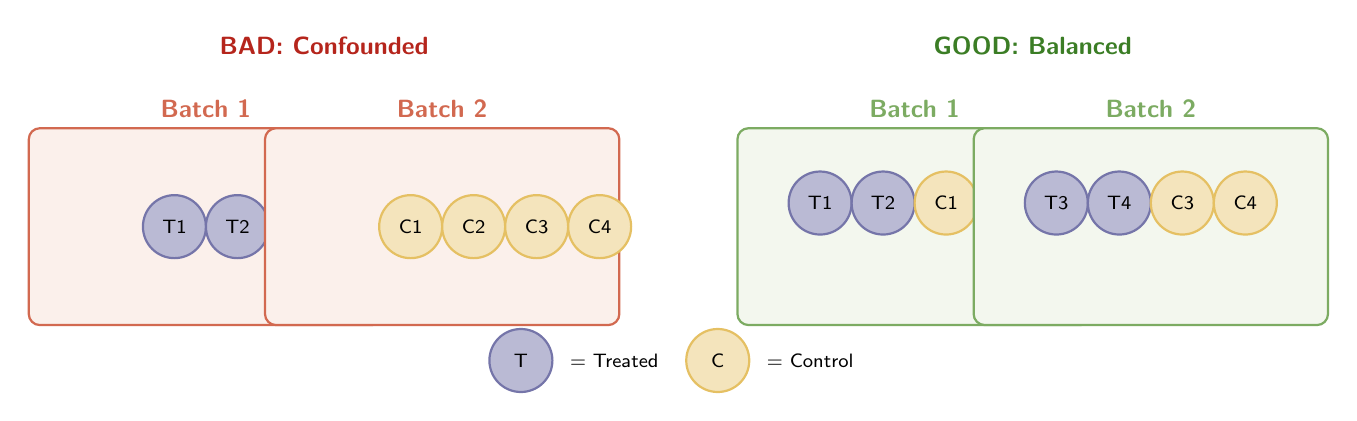
\begin{tikzpicture}[
  sample/.style={circle, draw, minimum size=0.8cm, font=\scriptsize\sffamily, thick},
  batch/.style={rectangle, draw, rounded corners=4pt, minimum width=4.5cm, minimum height=2.5cm, thick},
  label/.style={font=\small\sffamily\bfseries}
]

% BAD design
\node[label, BrickRed] at (-4.5, 3.5) {BAD: Confounded};
\node[batch, draw=BrickRed!60, fill=BrickRed!5] (b1bad) at (-6, 1.2) {};
\node[label, BrickRed!60, above] at (b1bad.north) {Batch 1};
\foreach \i in {1,...,4} {
  \node[sample, fill=MidnightBlue!30, draw=MidnightBlue!60] at (-7.2+\i*0.8, 1.2) {T\i};
}

\node[batch, draw=BrickRed!60, fill=BrickRed!5] (b2bad) at (-3, 1.2) {};
\node[label, BrickRed!60, above] at (b2bad.north) {Batch 2};
\foreach \i in {1,...,4} {
  \node[sample, fill=Goldenrod!30, draw=Goldenrod!70] at (-4.2+\i*0.8, 1.2) {C\i};
}

% GOOD design
\node[label, OliveGreen] at (4.5, 3.5) {GOOD: Balanced};
\node[batch, draw=OliveGreen!60, fill=OliveGreen!5] (b1good) at (3, 1.2) {};
\node[label, OliveGreen!60, above] at (b1good.north) {Batch 1};
\node[sample, fill=MidnightBlue!30, draw=MidnightBlue!60] at (1.8, 1.5) {T1};
\node[sample, fill=MidnightBlue!30, draw=MidnightBlue!60] at (2.6, 1.5) {T2};
\node[sample, fill=Goldenrod!30, draw=Goldenrod!70] at (3.4, 1.5) {C1};
\node[sample, fill=Goldenrod!30, draw=Goldenrod!70] at (4.2, 1.5) {C2};

\node[batch, draw=OliveGreen!60, fill=OliveGreen!5] (b2good) at (6, 1.2) {};
\node[label, OliveGreen!60, above] at (b2good.north) {Batch 2};
\node[sample, fill=MidnightBlue!30, draw=MidnightBlue!60] at (4.8, 1.5) {T3};
\node[sample, fill=MidnightBlue!30, draw=MidnightBlue!60] at (5.6, 1.5) {T4};
\node[sample, fill=Goldenrod!30, draw=Goldenrod!70] at (6.4, 1.5) {C3};
\node[sample, fill=Goldenrod!30, draw=Goldenrod!70] at (7.2, 1.5) {C4};

% Legend
\node[sample, fill=MidnightBlue!30, draw=MidnightBlue!60] at (-2, -0.5) {T};
\node[font=\scriptsize\sffamily, right] at (-1.5, -0.5) {= Treated};
\node[sample, fill=Goldenrod!30, draw=Goldenrod!70] at (0.5, -0.5) {C};
\node[font=\scriptsize\sffamily, right] at (1.0, -0.5) {= Control};

\end{tikzpicture}
\caption[Balanced batch design.]{Left: a confounded design where batch and condition are indistinguishable. Right: a balanced design where both conditions are represented in every batch. The balanced design allows batch effects to be estimated and removed computationally.}
\label{fig:batch-design}
\end{figure}

\subsection{Computational Batch Effect Correction}

When batch effects cannot be completely prevented (e.g., multi-site studies, longitudinal experiments), they can be mitigated computationally---but only if batch is not confounded with condition:

\begin{description}[style=nextline, font=\bfseries, itemsep=3pt]
  \item[ComBat / ComBat-seq]
  Empirical Bayes framework for batch correction. ComBat works on normalized data; ComBat-seq works directly on count matrices (preferred for RNA-seq). Available in the \texttt{sva} R package.

  \item[limma::removeBatchEffect]
  Adjusts expression values for known batch variables. Useful for visualization (PCA, heatmaps) but not for differential expression testing---instead, include batch as a covariate in the DESeq2 design formula.

  \item[Harmony]
  Fast integration method for single-cell data. Corrects batch effects in PCA space, preserving biological variation. Widely used for integrating scRNA-seq datasets from different experiments or technologies.

  \item[Scanorama / scVI / BBKNN]
  Alternative single-cell integration methods. scVI uses a variational autoencoder; BBKNN modifies the nearest-neighbor graph. Each has different strengths depending on the severity of batch effects.
\end{description}

\begin{warningbox}[title={Batch Correction Cannot Fix Confounded Designs}]
If batch is perfectly confounded with the biological condition of interest (all treated samples in batch 1, all controls in batch 2), no computational method can distinguish biological effects from batch effects. The results will be unreliable regardless of how sophisticated the correction. Prevention through balanced experimental design is the only solution.
\end{warningbox}

%=============================================================================
\section{Controls}
\label{sec:expdesign:controls}
%=============================================================================

Appropriate controls are essential for distinguishing true signal from background noise and technical artefacts.

\subsection{Sequencing Controls}

\begin{description}[style=nextline, font=\bfseries, itemsep=3pt]
  \item[PhiX spike-in]
  A balanced-composition bacteriophage genome library included at 1--5\% in every Illumina sequencing run. PhiX serves as a quality control: it provides an independent estimate of error rate, helps with color calibration, and boosts sequence diversity for low-complexity libraries. For amplicon sequencing on two-channel instruments (NextSeq, NovaSeq X), spike in 20--50\% PhiX.

  \item[Negative controls (no-template controls)]
  Process a ``blank'' sample (water or empty well) through the entire library preparation and sequencing workflow. Contamination in the negative control reveals kit reagent contamination or cross-contamination during processing. Critical for low-input protocols and metagenomics.

  \item[Positive controls]
  Include a well-characterised reference sample with known properties. Examples: the NA12878/HG001 reference genome for WGS variant calling validation, ERCC spike-in RNA mixes for RNA-seq, or a mock microbial community for 16S metagenomics.
\end{description}

\subsection{Assay-Specific Controls}

\begin{description}[style=nextline, font=\bfseries, itemsep=3pt]
  \item[Input control (ChIP-seq)]
  Chromatin that has been cross-linked and sonicated but not immunoprecipitated. Serves as the background model for peak calling. Essential for ChIP-seq; typically not needed for CUT\&Tag (which uses IgG control or no-antibody control instead).

  \item[ERCC spike-ins (RNA-seq)]
  External RNA Controls Consortium (ERCC) synthetic RNA molecules added at known concentrations before library preparation. Enable assessment of technical variation, detection sensitivity, and (with appropriate normalization) absolute quantification.

  \item[Spike-in normalization (CUT\&Tag)]
  \species{Escherichia coli} DNA carried over from the pA-Tn5 production in CUT\&Tag experiments can serve as a spike-in for normalization. Alternatively, \species{Drosophila} chromatin can be added as an exogenous spike-in for cross-sample normalization.

  \item[Synthetic methylation standards (WGBS)]
  Fully methylated and fully unmethylated lambda phage or synthetic DNA spike-ins to assess bisulfite conversion efficiency. Conversion rates should exceed 99\%.
\end{description}

%=============================================================================
\section{Multiplexing Strategy}
\label{sec:expdesign:multiplexing}
%=============================================================================

Multiplexing allows multiple samples to be sequenced on the same flow cell by adding unique index (barcode) sequences to each library. Proper multiplexing strategy is critical for cost-effective and accurate sequencing.

\subsection{How Many Samples per Flow Cell}

The number of samples that can be multiplexed depends on the required depth per sample and the flow cell output:

\begin{equation}
\text{Number of samples} = \frac{\text{Flow cell output (reads)}}{\text{Required reads per sample}}
\end{equation}

For example, an Illumina NovaSeq X 10B flow cell produces approximately 10--13 billion read pairs with a 2$\times$150\basepair{} run, corresponding to roughly 3--4~Tb of sequence. A 3~Gb human genome at 30$\times$ mean coverage requires about 90~Gb, or approximately 300 million 2$\times$150 read pairs before allowing for duplicates, unusable reads, and coverage non-uniformity. The theoretical capacity is therefore about 33--43 human genomes, and practical pooling should be lower. By contrast, 10 billion read pairs could support about 333 RNA-seq libraries at 30 million read pairs each. Always calculate pooling from bases required and the current vendor specification; the flow-cell name is not itself a guaranteed read count.

\subsection{Index Compatibility and Distance}

Multiplexed libraries must have index sequences that are sufficiently different from each other to prevent misassignment. Key considerations:

\begin{itemize}[itemsep=2pt]
  \item \textbf{Hamming distance:} Use indexes with a minimum Hamming distance of 3 (at least 3 positions differ), enabling 1-error correction.
  \item \textbf{Color balance:} On two-channel Illumina instruments, ensure that each cycle of the index read has a mixture of labelled and unlabelled bases (balanced A/C and G/T ratios).
  \item \textbf{Unique dual indexes (UDIs):} On patterned flow cells (NovaSeq, NextSeq 1000/2000), use UDIs---unique combinations of i7 and i5 indexes---to prevent index hopping. Combinatorial dual indexing (reusing the same i7 with different i5 across samples) is vulnerable to hopping on these platforms.
\end{itemize}

\begin{warningbox}[title={Index Hopping on Patterned Flow Cells}]
On patterned flow cells that use exclusion amplification (ExAmp), free adapter molecules can hybridize to the wrong nanowell, causing reads to be assigned to the wrong sample (``index hopping''). Rates of 0.1--2\% have been reported. Use unique dual indexes (UDIs) rather than combinatorial dual indexes. Libraries from unrelated projects sharing a flow cell should be especially careful.
\end{warningbox}

%=============================================================================
\section{Sample Collection and Storage}
\label{sec:expdesign:samples}
%=============================================================================

The quality of sequencing results ultimately depends on the quality of the starting material. Nucleic acids are fragile molecules that can be degraded by nucleases, heat, pH extremes, and repeated freeze-thaw cycles.

\subsection{DNA Storage}

\begin{itemize}[itemsep=2pt]
  \item \textbf{Fresh tissue:} Snap-freeze in liquid nitrogen immediately after collection. Store at $-80$\textdegree{}C.
  \item \textbf{Blood:} Collect in EDTA tubes (EDTA inhibits nucleases). Process within 24 hours or freeze.
  \item \textbf{FFPE (formalin-fixed, paraffin-embedded):} Standard for pathology archives. DNA from FFPE is degraded and chemically modified; special extraction kits and library preparation protocols are required. Expect shorter fragments and higher error rates.
  \item \textbf{Extracted DNA:} Store in TE buffer (10~mM Tris, 1~mM EDTA, pH 8.0) at $-20$\textdegree{}C for long-term storage or 4\textdegree{}C for short-term use. Avoid repeated freeze-thaw cycles.
\end{itemize}

\subsection{RNA Storage}

RNA is much more labile than DNA due to the ubiquity of RNases:

\begin{itemize}[itemsep=2pt]
  \item \textbf{Fresh tissue:} Snap-freeze immediately or place in \textbf{RNAlater} (a stabilization reagent that penetrates tissue and inactivates RNases). RNAlater-preserved samples can be stored at room temperature for up to one week, or at $-80$\textdegree{}C for long-term storage.
  \item \textbf{Cultured cells:} Lyse directly in TRIzol or equivalent extraction reagent. Do not pellet cells and freeze without stabilization.
  \item \textbf{Blood RNA:} Collect in PAXgene or Tempus RNA blood tubes, which lyse cells and stabilize RNA immediately upon collection.
  \item \textbf{FFPE:} RNA from FFPE is highly degraded. The RNA Integrity Number (RIN) is typically $<$3 (vs 8--10 for high-quality RNA). Use FFPE-specific library preparation kits.
\end{itemize}

\begin{tipbox}[title={RNA Quality Assessment}]
Always assess RNA quality before library preparation using the Agilent Bioanalyzer, TapeStation, or equivalent. The \textbf{RNA Integrity Number (RIN)} ranges from 1 (fully degraded) to 10 (intact). For standard RNA-seq, a RIN $\geq$ 7 is recommended. Some protocols (e.g., ribosomal RNA depletion) can handle more degraded RNA (RIN 3--7), but expect reduced data quality.
\end{tipbox}

%=============================================================================
\section{Cost Estimation and Budgeting}
\label{sec:expdesign:cost}
%=============================================================================

A realistic budget for an NGS experiment must account for all components of the workflow:

\begin{enumerate}[itemsep=2pt]
  \item \textbf{Sample collection and processing:} IRB approval, sample collection supplies, nucleic acid extraction kits.
  \item \textbf{Quality assessment:} Bioanalyzer/TapeStation chips (\$15--30 per sample), Qubit assays (\$2--5 per sample).
  \item \textbf{Library preparation:} \$50--200 per sample depending on the kit and protocol.
  \item \textbf{Sequencing:} The largest variable cost, ranging from \$50 per sample (low-coverage WGS or RNA-seq on a high-throughput instrument) to \$500+ (deep WGS on an individual flow cell).
  \item \textbf{Computational:} HPC time, cloud computing charges, data storage (\$20--30 per TB per month for cloud storage).
  \item \textbf{Personnel:} Bioinformatics analyst time is often the largest hidden cost.
\end{enumerate}

\begin{tipbox}[title={Get Core Facility Quotes}]
Contact your institutional sequencing core facility or commercial provider early in the planning process. Core facilities can provide accurate per-sample costs, advise on multiplexing strategies, and often handle library preparation and QC. Commercial services (Novogene, BGI, Genewiz/Azenta, etc.) may offer lower per-sample costs for large projects.
\end{tipbox}

%=============================================================================
\section{Decision Tree for Choosing a Sequencing Strategy}
\label{sec:expdesign:decision}
%=============================================================================

\begin{figure}[htbp]
\centering
\resizebox{\textwidth}{!}{%
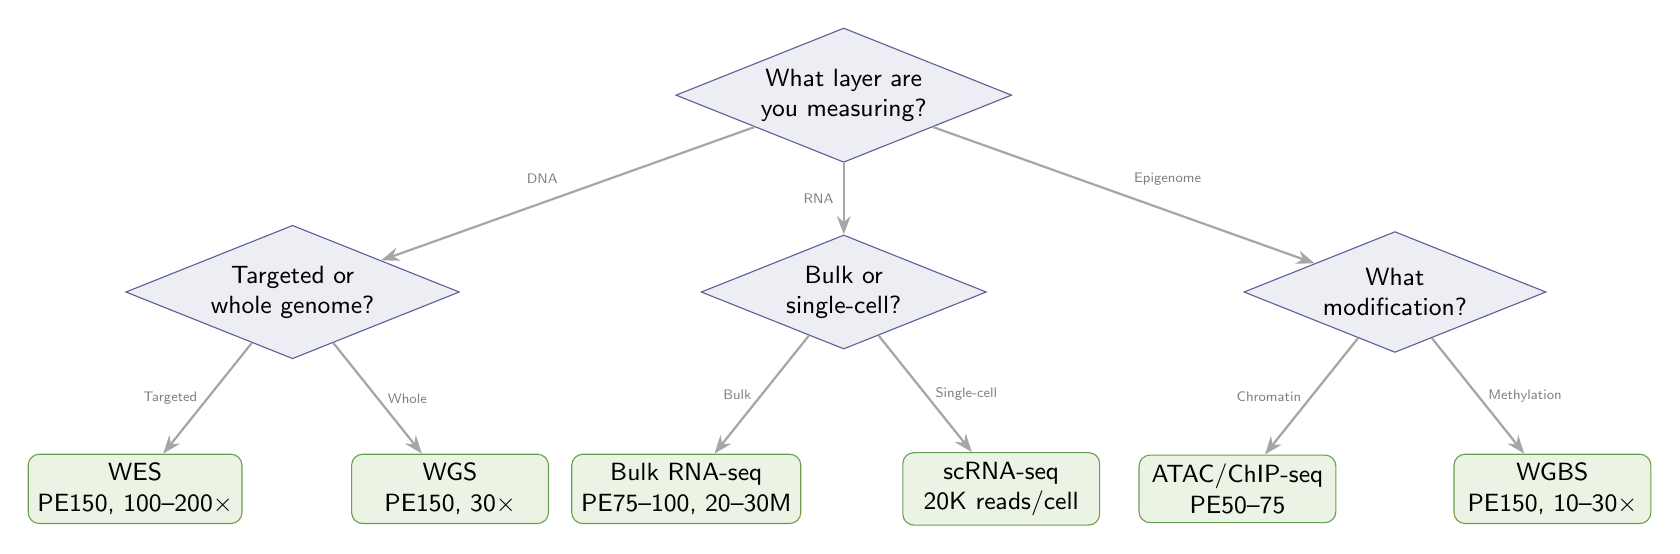
\begin{tikzpicture}[
  decision/.style={diamond, draw=MidnightBlue!70, fill=MidnightBlue!8,
    inner sep=2pt, aspect=2.5, align=center, font=\small\sffamily},
  result/.style={rectangle, draw=OliveGreen!70, fill=OliveGreen!8,
    rounded corners=4pt, minimum height=0.7cm, align=center, font=\small\sffamily,
    minimum width=2.5cm},
  arr/.style={-{Stealth}, thick, gray!70},
  lbl/.style={font=\tiny\sffamily, text=gray}
]

\node[decision] (q1) at (0,0) {What layer are\\you measuring?};

\node[decision] (q2a) at (-7,-2.5) {Targeted or\\whole genome?};
\node[decision] (q2b) at (0,-2.5) {Bulk or\\single-cell?};
\node[decision] (q2c) at (7,-2.5) {What\\modification?};

% DNA branch
\node[result] (r1) at (-9,-5) {WES\\PE150, 100--200$\times$};
\node[result] (r2) at (-5,-5) {WGS\\PE150, 30$\times$};

% RNA branch
\node[result] (r3) at (-2,-5) {Bulk RNA-seq\\PE75--100, 20--30M};
\node[result] (r4) at (2,-5) {scRNA-seq\\20K reads/cell};

% Epigenome branch
\node[result] (r5) at (5,-5) {ATAC/ChIP-seq\\PE50--75};
\node[result] (r6) at (9,-5) {WGBS\\PE150, 10--30$\times$};

\draw[arr] (q1) -- node[lbl, above left] {DNA} (q2a);
\draw[arr] (q1) -- node[lbl, left] {RNA} (q2b);
\draw[arr] (q1) -- node[lbl, above right] {Epigenome} (q2c);

\draw[arr] (q2a) -- node[lbl, left] {Targeted} (r1);
\draw[arr] (q2a) -- node[lbl, right] {Whole} (r2);
\draw[arr] (q2b) -- node[lbl, left] {Bulk} (r3);
\draw[arr] (q2b) -- node[lbl, right] {Single-cell} (r4);
\draw[arr] (q2c) -- node[lbl, left] {Chromatin} (r5);
\draw[arr] (q2c) -- node[lbl, right] {Methylation} (r6);

\end{tikzpicture}%
}
\caption[Sequencing strategy decision tree.]{Simplified decision tree for selecting a sequencing strategy. Start with the biological layer of interest, then refine based on scope (whole-genome vs targeted) and resolution (bulk vs single-cell).}
\label{fig:exp-decision-tree}
\end{figure}

%=============================================================================
\section{Comprehensive Experimental Design Reference Table}
\label{sec:expdesign:mastertable}
%=============================================================================

\begin{table}[htbp]
\centering
\caption{Master experimental design reference: depth, replicates, read length, and key considerations for common NGS assays.}
\label{tab:master-design}
\small
\renewcommand{\arraystretch}{1.2}
\begin{tabularx}{\textwidth}{@{}l c c c X@{}}
\toprule
\textbf{Assay} & \textbf{Depth} & \textbf{Replicates} & \textbf{Read Config} & \textbf{Key Design Notes} \\
\midrule
WGS (germline) & 30$\times$ & 1/individual & PE150 & Matched normal for somatic analysis \\
WGS (somatic) & 60--100$\times$ & 1 T + 1 N & PE150 & Higher depth for low-frequency variants \\
WES & 100--200$\times$ & 1/individual & PE100--150 & Account for capture uniformity \\
RNA-seq (DE) & 20--30M & 3--5+/condition & PE75--100 & Prioritize replicates over depth \\
RNA-seq (isoform) & 50--100M & 3+/condition & PE150 & Long reads help with novel isoforms \\
scRNA-seq & 20--50K/cell & 2+/condition & R1:28, R2:91 & More cells usually beats more depth \\
ATAC-seq & 50--75M unique & 2--3/condition & PE50--75 & Remove mitochondrial reads \\
ChIP-seq (narrow) & 20--40M & 2/condition & SE50--75 & Input control required \\
ChIP-seq (broad) & 40--60M & 2/condition & PE75 & Broad peaks need more reads \\
CUT\&Tag & 3--8M & 2/condition & PE50 & Very low background; spike-in norm. \\
WGBS & 10--30$\times$ & 2--3/condition & PE100--150 & Check bisulfite conversion rate \\
Hi-C & 50M--2B & 1--2 & PE50--150 & Depth determines resolution \\
16S amplicon & 10--100K/sample & 5--10+ & PE250--300 & Must overlap for amplicon assembly \\
\bottomrule
\end{tabularx}
\end{table}

%=============================================================================
\section{Summary}
\label{sec:expdesign:summary}
%=============================================================================

Effective experimental design for NGS experiments requires careful consideration of multiple interacting factors:

\begin{itemize}[itemsep=2pt]
  \item \textbf{Replication:} Biological replicates are essential; technical replicates are usually unnecessary. The minimum number of replicates depends on the assay and the effect size you need to detect.
  \item \textbf{Sequencing depth:} Must be matched to the application. Too little depth misses signal; too much wastes resources. When in doubt, more replicates at moderate depth outperform fewer replicates at higher depth.
  \item \textbf{Read length:} Choose based on the application. PE150 is the standard for WGS; shorter reads (PE50--100) are sufficient for many assays.
  \item \textbf{Power analysis:} Perform before the experiment to size the study appropriately. Tools like RNASeqPower and powsimR make this straightforward.
  \item \textbf{Batch effects:} The most common preventable source of error. Balance conditions across batches and never confound batch with condition.
  \item \textbf{Controls:} Include appropriate controls for every experiment---PhiX for sequencing QC, input/IgG for ChIP-seq, ERCC spike-ins for RNA-seq, negative controls for contamination detection.
  \item \textbf{Multiplexing:} Use unique dual indexes on patterned flow cells. Ensure index compatibility and color balance.
  \item \textbf{Sample quality:} Invest in proper sample collection, storage, and nucleic acid extraction. No amount of sequencing can rescue degraded samples.
\end{itemize}

Planning the experiment carefully before the first sample is collected is the single most impactful action you can take to ensure your sequencing project succeeds.

\chapter{Data Standards, Sharing, and Reproducibility}
\label{ch:datastandards}

\begin{keyconcept}
Genomics data has maximal value when it is shared openly, described with rich metadata, stored in standardised formats, and produced by reproducible methods. Data sharing is not merely a journal requirement---it is a fundamental pillar of the scientific process that enables reuse, meta-analysis, validation, and discovery far beyond the original study. This chapter describes the repositories, standards, and best practices for making NGS data findable, accessible, interoperable, and reusable.
\end{keyconcept}

\section{Why Data Sharing and Standards Matter}
\label{sec:datastandards:why}

The genomics community generates petabytes of data annually. Without standards and public repositories, this data would be siloed in individual laboratories, inaccessible for reuse, and lost when hard drives fail or students graduate. The benefits of data sharing are substantial:

\begin{itemize}[itemsep=2pt]
  \item \textbf{Reproducibility:} Independent researchers can verify published results using the original data.
  \item \textbf{Discovery:} Public datasets enable new analyses that the original authors did not envision. Many high-impact papers are entirely based on re-analysis of public data.
  \item \textbf{Meta-analysis:} Combining data across studies increases statistical power and reveals patterns invisible in individual datasets.
  \item \textbf{Training resources:} Public data provides invaluable training material for bioinformatics education.
  \item \textbf{Cost savings:} Reusing existing data avoids redundant sequencing of the same biological materials.
  \item \textbf{Equity:} Open data enables researchers in resource-limited settings to participate in cutting-edge genomics research.
\end{itemize}

Most funding agencies (NIH, ERC, Wellcome Trust, BBSRC, DFG) and journals (Nature, Science, Cell, PNAS, Genome Biology, etc.) now mandate data deposition in public repositories as a condition of funding or publication.

%=============================================================================
\section{Public Repositories for Raw Sequencing Data}
\label{sec:datastandards:raw}
%=============================================================================

\subsection{The International Nucleotide Sequence Database Collaboration (INSDC)}

The three primary archives for raw sequencing data are part of the INSDC, which synchronizes data globally:

\begin{description}[style=nextline, font=\bfseries, itemsep=4pt]
  \item[NCBI SRA (Sequence Read Archive)]
  The largest raw sequencing data archive, hosted by the US National Center for Biotechnology Information. SRA stores raw reads in a compressed format and provides programmatic access via the SRA Toolkit. As of 2026, SRA contains over 80 petabases of data from millions of experiments.

  \item[ENA (European Nucleotide Archive)]
  The European counterpart to SRA, hosted by EMBL-EBI. ENA stores the same data (mirrored from SRA) and provides a more flexible submission interface. ENA additionally stores assembled sequences and functional annotations.

  \item[DDBJ (DNA Data Bank of Japan)]
  Japan's nucleotide archive, operated by the National Institute of Genetics. Also mirrors INSDC data.
\end{description}

Data submitted to any one of these archives is automatically shared with the other two within 24--48 hours. You only need to submit once.

\subsection{How to Submit Data to SRA/ENA}

Data submission requires three levels of metadata organized in a hierarchical structure:

\begin{enumerate}[itemsep=2pt]
  \item \textbf{BioProject:} A top-level umbrella describing the overall research project. Contains a title, description, and organism. Each publication typically corresponds to one BioProject.
  \item \textbf{BioSample:} Describes each biological sample (organism, tissue type, genotype, treatment, collection date). One BioSample per biological unit (e.g., per patient, per cell line).
  \item \textbf{Experiment / Run:} Links a BioSample to a library preparation strategy and sequencing run. Contains library metadata (insert size, read length, platform, instrument model) and the actual FASTQ files.
\end{enumerate}

\begin{lstlisting}[language=bash,caption={Submitting data to SRA using the SRA Toolkit.},label=lst:sra-submit]
# Register BioProject and BioSamples via NCBI Submission Portal
# https://submit.ncbi.nlm.nih.gov/

# Upload FASTQ files using the SRA submission tool or Aspera
# Using Aspera (much faster than FTP for large files)
ascp -i ~/.aspera/connect/etc/asperaweb_id_dsa.openssh \
  -QT -l 1000m -k 1 \
  sample1_R1.fastq.gz sample1_R2.fastq.gz \
  subasp@upload.ncbi.nlm.nih.gov:uploads/your_key_folder/

# Alternative: submit via ENA using their Webin-CLI tool
java -jar webin-cli.jar -context reads \
  -manifest manifest.txt \
  -userName Webin-XXXXX -password XXXXX \
  -submit
\end{lstlisting}

\subsection{How to Download Data from SRA/ENA}

\begin{lstlisting}[language=bash,caption={Downloading data from SRA.},label=lst:sra-download]
# Using fasterq-dump (faster successor to fastq-dump)
fasterq-dump --split-files --threads 8 SRR12345678
# Produces: SRR12345678_1.fastq and SRR12345678_2.fastq
gzip SRR12345678_*.fastq

# Download multiple accessions with a loop
while read acc; do
  fasterq-dump --split-files --threads 8 "$acc"
  gzip "${acc}"_*.fastq
done < accession_list.txt

# Alternative: download directly from ENA (already in FASTQ format)
wget ftp://ftp.sra.ebi.ac.uk/vol1/fastq/SRR123/078/SRR12345678/SRR12345678_1.fastq.gz

# Programmatic access with pysradb (Python)
pip install pysradb
pysradb metadata --detailed SRP123456
pysradb download -t 8 SRP123456
\end{lstlisting}

\begin{tipbox}[title={ENA vs SRA for Downloads}]
Downloading from ENA is often faster and more convenient than from SRA, because ENA provides files directly in FASTQ format (no conversion needed), while SRA stores data in its own SRA format requiring conversion with \texttt{fasterq-dump}. ENA also provides direct FTP and Aspera download links.
\end{tipbox}

\subsection{Snakemake Workflow for SRA Data Download}

\begin{lstlisting}[language=Python,caption={Snakemake workflow for downloading SRA data.},label=lst:smk-sra]
# Snakefile -- Download data from SRA
configfile: "config.yaml"

ACCESSIONS = config["sra_accessions"]

rule all:
    input:
        expand("data/{acc}_1.fastq.gz", acc=ACCESSIONS),
        expand("data/{acc}_2.fastq.gz", acc=ACCESSIONS)

rule download_sra:
    output:
        r1="data/{acc}_1.fastq.gz",
        r2="data/{acc}_2.fastq.gz"
    threads: 8
    conda: "envs/sra.yaml"
    shell:
        """
        fasterq-dump --split-files --threads {threads} \
          --outdir data/ {wildcards.acc}
        gzip data/{wildcards.acc}_1.fastq
        gzip data/{wildcards.acc}_2.fastq
        """
\end{lstlisting}

\subsection{Nextflow Workflow for SRA Data Download}

\begin{lstlisting}[language=Java,caption={Nextflow process for downloading SRA data.},label=lst:nf-sra]
#!/usr/bin/env nextflow
nextflow.enable.dsl = 2

params.accessions = "accession_list.txt"
params.outdir     = "data"

process DOWNLOAD_SRA {
    tag "${accession}"
    publishDir "${params.outdir}", mode: 'copy'
    cpus 8

    input:  val(accession)
    output: tuple val(accession), path("*.fastq.gz"), emit: fastq

    script:
    """
    fasterq-dump --split-files --threads ${task.cpus} ${accession}
    gzip *.fastq
    """
}

workflow {
    accessions_ch = Channel
        .fromPath(params.accessions)
        .splitText()
        .map { it.trim() }

    DOWNLOAD_SRA(accessions_ch)
}
\end{lstlisting}

%=============================================================================
\section{Processed Data Repositories}
\label{sec:datastandards:processed}
%=============================================================================

Beyond raw sequencing data, processed results (gene expression matrices, called peaks, variant lists) are deposited in specialized repositories:

\subsection{Gene Expression Omnibus (GEO)}

NCBI GEO is the most widely used repository for processed functional genomics data. A GEO submission typically includes:
\begin{itemize}[nosep]
  \item Processed data files (count matrices, normalized expression values, peak files)
  \item Sample metadata (conditions, treatments, organism, tissue)
  \item A link to the corresponding SRA submission for raw data
\end{itemize}

GEO assigns \textbf{GSE} accessions (for series/datasets) and \textbf{GSM} accessions (for individual samples). Researchers can browse and download GEO data via the web interface or programmatically using the \texttt{GEOquery} R package.

\subsection{ArrayExpress / BioStudies}

EMBL-EBI's equivalent to GEO, now transitioning to the BioStudies platform. ArrayExpress/BioStudies stores processed data with rich metadata in the MAGE-TAB format. Data is cross-referenced with ENA for raw reads.

\subsection{Consortium Data Portals}

Several large-scale consortia maintain their own data portals with curated, consistently processed datasets:

\begin{description}[style=nextline, font=\bfseries, itemsep=3pt]
  \item[ENCODE (Encyclopedia of DNA Elements)]
  Gold-standard ChIP-seq, ATAC-seq, RNA-seq, and Hi-C datasets with uniform processing pipelines. The ENCODE portal (\texttt{encodeproject.org}) provides downloadable processed files (BigWig, BED, BAM) and comprehensive quality metrics. ENCODE data quality standards serve as benchmarks for the field.

  \item[Roadmap Epigenomics]
  Comprehensive epigenomic maps (histone modifications, DNA methylation, chromatin accessibility) across 111 human tissues and cell types. Data available from the Roadmap Epigenomics portal.

  \item[GTEx (Genotype-Tissue Expression)]
  Gene expression data across 54 human tissues from nearly 1,000 post-mortem donors. GTEx is the primary resource for understanding tissue-specific gene expression and expression quantitative trait loci (eQTLs).

  \item[TCGA / GDC (The Cancer Genome Atlas / Genomic Data Commons)]
  Multi-omics data (WGS, WES, RNA-seq, methylation, miRNA, proteomics) for over 11,000 tumors across 33 cancer types. Accessible through the NCI Genomic Data Commons portal. Some data requires dbGaP access approval due to patient privacy.

  \item[Human Cell Atlas (HCA)]
  A global effort to create reference single-cell maps of every cell type in the human body. Data available through the HCA Data Portal.

  \item[CellxGene]
  A platform maintained by the Chan Zuckerberg Initiative for exploring and downloading curated single-cell datasets. Provides interactive visualization and standardized AnnData (h5ad) downloads.

  \item[UCSC Genome Browser and Table Browser]
  Comprehensive genome annotations, conservation tracks, regulatory elements, and variation data. The Table Browser allows bulk download of genomic tracks in BED, BigWig, and other formats.

  \item[Ensembl and BioMart]
  Genome annotations, gene models, orthology information, and variation data for hundreds of species. BioMart provides a powerful query interface for programmatic data retrieval.
\end{description}

%=============================================================================
\section{Reference Genomes and Annotations}
\label{sec:datastandards:references}
%=============================================================================

Consistent use of reference genomes and gene annotations is essential for reproducibility and cross-study comparability.

\subsection{Where to Download References}

\begin{description}[style=nextline, font=\bfseries, itemsep=3pt]
  \item[GENCODE]
  The gold standard for human and mouse gene annotations. Provides comprehensive annotations including protein-coding genes, lncRNAs, pseudogenes, and other non-coding elements. Available from \texttt{gencodegenes.org}. Current release: GENCODE v46 (human) based on GRCh38.

  \item[Ensembl]
  Annotations for hundreds of species. Ensembl annotations for human are closely related to GENCODE but follow a different release numbering. Available from \texttt{ensembl.org}.

  \item[RefSeq (NCBI)]
  NCBI's curated reference sequence database. RefSeq annotations tend to be more conservative (fewer predicted transcripts) than GENCODE. Used in clinical settings where annotation confidence is prioritized.

  \item[UCSC Genome Browser]
  Downloads for genome sequences, annotations, and tracks at \texttt{hgdownload.soe.ucsc.edu}.
\end{description}

\subsection{GENCODE vs RefSeq}

\begin{table}[htbp]
\centering
\caption{Comparison of GENCODE and RefSeq annotations.}
\label{tab:gencode-vs-refseq}
\small
\begin{tabularx}{\textwidth}{@{}l X X@{}}
\toprule
\textbf{Feature} & \textbf{GENCODE} & \textbf{RefSeq} \\
\midrule
Provider & EMBL-EBI / Wellcome Sanger & NCBI \\
Approach & Comprehensive (manual + automated) & Curated (conservative) \\
Transcript count & Higher (more predicted isoforms) & Lower (more stringent evidence) \\
Identifier format & ENSG/ENST (Ensembl IDs) & NM\_, NR\_, XM\_ (RefSeq IDs) \\
Non-coding genes & Extensive annotation & More conservative \\
Clinical use & Research standard & Often preferred in clinical settings \\
Update frequency & Biannual releases & Continuous updates \\
\bottomrule
\end{tabularx}
\end{table}

\begin{warningbox}[title={Mixing References Is Dangerous}]
Never mix genome builds or annotation versions within a single analysis. Using a GRCh37 VCF with a GRCh38 annotation file, or a GENCODE GTF with RefSeq gene names, can produce incorrect or uninterpretable results. Document the exact genome build, annotation source, and release version in every analysis.
\end{warningbox}

\subsection{Genome Builds and LiftOver}

When comparing results across studies that used different genome builds (e.g., GRCh37/hg19 vs GRCh38/hg38), coordinate conversion is necessary:

\begin{lstlisting}[language=bash,caption={Converting coordinates between genome builds with liftOver.},label=lst:liftover]
# Download the chain file for hg19 -> hg38 conversion
wget https://hgdownload.soe.ucsc.edu/goldenPath/hg19/liftOver/hg19ToHg38.over.chain.gz

# Convert BED coordinates from hg19 to hg38
liftOver input_hg19.bed hg19ToHg38.over.chain.gz \
  output_hg38.bed unmapped.bed

# In R, use rtracklayer
library(rtracklayer)
chain <- import.chain("hg19ToHg38.over.chain")
gr_hg38 <- liftOver(gr_hg19, chain)
\end{lstlisting}

%=============================================================================
\section{Metadata Standards}
\label{sec:datastandards:metadata}
%=============================================================================

Metadata---data about data---is what makes raw sequencing files interpretable. Without knowing the organism, tissue type, experimental condition, library preparation method, and sequencing parameters, a FASTQ file is just a meaningless stream of letters.

\subsection{Key Metadata Standards}

\begin{description}[style=nextline, font=\bfseries, itemsep=3pt]
  \item[MINSEQE (Minimum Information about a high-throughput Nucleotide Sequencing Experiment)]
  The community standard for NGS metadata, analogous to MIAME for microarrays. MINSEQE specifies the minimum information needed to interpret and reproduce a sequencing experiment: (1) raw data, (2) processed data, (3) experiment design including sample descriptions, (4) experimental protocols, and (5) data processing protocols.

  \item[MIAME (Minimum Information About a Microarray Experiment)]
  The historical predecessor to MINSEQE, established for microarray experiments. Many of its principles apply to sequencing experiments.

  \item[Dublin Core]
  A general-purpose metadata standard (title, creator, date, description, identifier) used for cataloguing research outputs. Forms the basis for many repository metadata schemas.
\end{description}

\subsection{Ontologies for Standardized Terminology}

Free-text metadata fields (e.g., ``brain tissue,'' ``brain,'' ``cerebral cortex'') create inconsistencies that hinder data integration. Ontologies provide controlled vocabularies:

\begin{description}[style=nextline, font=\bfseries, itemsep=3pt]
  \item[EFO (Experimental Factor Ontology)]
  Standardized terms for experimental variables: diseases, cell types, anatomical locations, organisms, and assay types. Used by GEO, ArrayExpress, and GWAS Catalog.

  \item[OBI (Ontology for Biomedical Investigations)]
  Terms for experimental protocols, instruments, and data transformation processes.

  \item[CL (Cell Ontology)]
  Standardized cell type names. Essential for single-cell studies where consistent cell type labelling is critical for cross-study comparisons.

  \item[UBERON]
  Cross-species anatomical ontology. Enables comparison of tissues across organisms (e.g., human ``liver'' maps to mouse ``liver'').
\end{description}

%=============================================================================
\section{FAIR Principles}
\label{sec:datastandards:fair}
%=============================================================================

The \textbf{FAIR principles} provide a framework for making data maximally useful:

\begin{keyconcept}[title={FAIR Data Principles}]
\begin{description}[font=\bfseries, itemsep=3pt]
  \item[Findable] Data should have globally unique, persistent identifiers (DOIs, accession numbers). Rich metadata should be registered in searchable resources.
  \item[Accessible] Data should be retrievable using standardised, open protocols. Even if data access requires authentication (e.g., for patient data), the metadata should always be accessible.
  \item[Interoperable] Data should use standardised formats (FASTQ, BAM, VCF) and controlled vocabularies (ontologies). This enables integration across datasets and tools.
  \item[Reusable] Data should include clear provenance information, usage licenses, and detailed metadata following community standards. This enables meaningful reuse for new purposes.
\end{description}
\end{keyconcept}

For NGS data, FAIR compliance means:
\begin{itemize}[itemsep=2pt]
  \item Submitting raw data to SRA/ENA with complete BioProject/BioSample metadata.
  \item Using standard file formats (FASTQ, BAM, VCF, BED, BigWig) rather than custom formats.
  \item Providing processing code in public repositories (GitHub/GitLab) with DOIs (Zenodo).
  \item Using ontology terms rather than free text for sample descriptions.
  \item Publishing under open-access licenses when possible.
\end{itemize}

%=============================================================================
\section{Reproducibility in Bioinformatics}
\label{sec:datastandards:reproducibility}
%=============================================================================

Computational reproducibility---the ability to regenerate the same results from the same input data---remains a significant challenge in bioinformatics. Studies have shown that a large fraction of published bioinformatics analyses cannot be reproduced, even by the original authors, due to undocumented software versions, missing code, or unavailable data.

\subsection{Pillars of Computational Reproducibility}

\begin{enumerate}[itemsep=3pt]
  \item \textbf{Version pinning for software:} Record the exact version of every tool used. A Conda environment file (\texttt{environment.yml}) or container image digest provides this.

  \item \textbf{Version pinning for reference data:} Record the exact genome build (e.g., GRCh38 patch 14), annotation version (e.g., GENCODE v44), and database versions (e.g., dbSNP b156, gnomAD v4.0).

  \item \textbf{Containers (Docker, Singularity):} Package the complete software environment---operating system, libraries, and tools---into a portable, immutable image. The same container produces identical results regardless of the host system.

  \item \textbf{Workflow managers (Snakemake, Nextflow):} Encode the complete analysis pipeline as executable code. The workflow file serves as a precise, machine-readable protocol.

  \item \textbf{Literate programming:} Combine narrative, code, and results in a single document using R Markdown, Quarto, or Jupyter notebooks. This ensures that figures and tables in a manuscript can be traced directly to the code that generated them.

  \item \textbf{Code repositories:} Host all analysis code on GitHub or GitLab. Tag specific commits corresponding to publication versions.

  \item \textbf{Zenodo:} Archive code repositories on Zenodo to obtain a DOI. GitHub repositories can change or be deleted; Zenodo provides permanent archival with a citable DOI.
\end{enumerate}

\subsection{Example Reproducible Project Structure}

\begin{lstlisting}[caption={Recommended directory structure for a reproducible bioinformatics project.},label=lst:project-structure]
my_ngs_project/
|-- README.md                  # Project description and instructions
|-- LICENSE                    # Open-source license (e.g., MIT, GPL)
|-- Snakefile                  # Main Snakemake workflow (or main.nf)
|-- nextflow.config            # Nextflow configuration (if using NF)
|-- config.yaml                # Project-specific parameters
|-- envs/                      # Conda environment files
|   |-- align.yaml
|   |-- count.yaml
|   |-- deseq2.yaml
|-- containers/                # Dockerfiles (if not using Biocontainers)
|   |-- Dockerfile
|-- scripts/                   # Custom analysis scripts
|   |-- run_deseq2.R
|   |-- plot_figures.R
|   |-- run_scanpy.py
|-- notebooks/                 # Exploratory analyses
|   |-- exploration.Rmd
|   |-- qc_report.ipynb
|-- data/                      # Raw data (NOT committed to Git)
|   |-- README.md              # How to obtain the data
|-- ref/                       # Reference files (NOT committed to Git)
|   |-- README.md              # Download URLs and versions
|-- results/                   # Pipeline outputs (NOT committed to Git)
|-- .gitignore                 # Exclude data/, results/, ref/
\end{lstlisting}

\subsection{Snakemake Example for Reproducible Analysis}

\begin{lstlisting}[language=Python,caption={Snakemake workflow for a reproducible project with containers.},label=lst:smk-repro]
# Snakefile -- Reproducible analysis with containers
configfile: "config.yaml"

# Use Singularity containers for every rule
singularity: "docker://continuumio/miniconda3:latest"

rule all:
    input:
        "results/final_report.html"

rule align:
    input:
        r1="data/{sample}_R1.fastq.gz",
        r2="data/{sample}_R2.fastq.gz"
    output:
        "results/aligned/{sample}.bam"
    threads: 16
    container:
        "docker://biocontainers/bwa:v0.7.17_cv1"
    shell:
        """
        bwa mem -t {threads} {config[reference]} \
          {input.r1} {input.r2} \
          | samtools sort -o {output} -
        """

rule report:
    input:
        expand("results/aligned/{s}.bam", s=config["samples"])
    output:
        "results/final_report.html"
    container:
        "docker://rocker/tidyverse:4.3.2"
    script:
        "scripts/generate_report.Rmd"
\end{lstlisting}

\subsection{Nextflow Example for Reproducible Analysis}

\begin{lstlisting}[language=Java,caption={Nextflow workflow with container-based reproducibility.},label=lst:nf-repro]
#!/usr/bin/env nextflow
nextflow.enable.dsl = 2

params.reads  = "data/*_{R1,R2}.fastq.gz"
params.ref    = "ref/GRCh38.fa"
params.outdir = "results"

process ALIGN {
    container 'biocontainers/bwa:v0.7.17_cv1'
    cpus 16
    publishDir "${params.outdir}/aligned", mode: 'copy'

    input:
        tuple val(sample_id), path(reads)
        path(ref)

    output:
        tuple val(sample_id), path("*.sorted.bam"), emit: bam

    script:
    def (r1, r2) = reads
    """
    bwa mem -t ${task.cpus} ${ref} ${r1} ${r2} \
      | samtools sort -o ${sample_id}.sorted.bam -
    """
}

process REPORT {
    container 'rocker/tidyverse:4.3.2'
    publishDir "${params.outdir}", mode: 'copy'

    input:  path(bams)
    output: path("final_report.html")

    script:
    """
    Rscript -e "rmarkdown::render('${projectDir}/scripts/report.Rmd', \
      output_dir = '.')"
    """
}

workflow {
    reads_ch = Channel.fromFilePairs(params.reads, checkIfExists: true)
    ref_ch   = Channel.value(file(params.ref))

    ALIGN(reads_ch, ref_ch)
    REPORT(ALIGN.out.bam.map { it[1] }.collect())
}
\end{lstlisting}

%=============================================================================
\section{Data Management Plans}
\label{sec:datastandards:dmp}
%=============================================================================

Most funding agencies require a Data Management Plan (DMP) as part of grant applications. A DMP describes how data will be generated, managed, shared, and preserved.

\subsection{What Funding Agencies Require}

\begin{description}[style=nextline, font=\bfseries, itemsep=3pt]
  \item[NIH (USA)]
  Since January 2023, the NIH Data Management and Sharing Policy requires all funded research to submit a DMP describing: (1) data types generated, (2) data standards and metadata, (3) preservation and access plans, (4) timeline for sharing, and (5) oversight. Genomic data must be shared through approved repositories (SRA, GEO, dbGaP for controlled-access data).

  \item[ERC (European Research Council)]
  Requires compliance with the EU Open Science policy. Research data should be ``as open as possible, as closed as necessary.'' Open access to publications and FAIR data sharing are expected.

  \item[Wellcome Trust (UK)]
  Expects all research outputs, including data and code, to be shared openly. Requires a DMP and supports data deposition costs.
\end{description}

\subsection{Storage Considerations}

\begin{table}[htbp]
\centering
\caption{Typical data volumes and storage requirements for NGS projects.}
\label{tab:storage}
\small
\begin{tabularx}{\textwidth}{@{}l l l X@{}}
\toprule
\textbf{Data Type} & \textbf{Size per Sample} & \textbf{Compression} & \textbf{Storage Notes} \\
\midrule
FASTQ (30$\times$ WGS) & 60--90 Gb & gzip: 3--4$\times$ & Archive in SRA; delete local copies after verification \\
BAM (30$\times$ WGS) & 50--80 Gb & CRAM: 30--60\% smaller & Regenerable from FASTQ; archive or delete \\
VCF & 0.1--1 Gb & bgzip + tabix & Small; retain permanently \\
RNA-seq FASTQ & 3--8 Gb & gzip & Archive in SRA \\
scRNA-seq (h5ad) & 0.5--5 Gb & zlib compressed & Retain processed object \\
BigWig tracks & 0.1--1 Gb & Pre-compressed & Retain for visualization \\
\bottomrule
\end{tabularx}
\end{table}

\begin{tipbox}[title={Data Retention Strategy}]
Not all data needs to be kept permanently. Raw FASTQ files should be archived in SRA/ENA (free, permanent storage). Intermediate files (unsorted BAMs, temporary files) can be deleted after the pipeline completes. Final processed results (VCFs, count matrices, peak files) should be retained locally and deposited in GEO or equivalent. BAM files can often be regenerated from FASTQ, so consider deleting them after analysis if storage is limited.
\end{tipbox}

\subsection{Data Security and Patient Consent}

Genomic data from human subjects requires careful attention to privacy and consent:

\begin{description}[style=nextline, font=\bfseries, itemsep=3pt]
  \item[HIPAA (USA)]
  The Health Insurance Portability and Accountability Act governs the use and disclosure of protected health information. Genomic data linked to patient identifiers is subject to HIPAA. De-identification is required for open sharing; controlled-access repositories (dbGaP) are used for data that cannot be fully de-identified.

  \item[GDPR (EU)]
  The General Data Protection Regulation classifies genetic data as ``special category'' personal data, subject to strict processing requirements. Explicit consent, data minimization, and purpose limitation principles apply. Cross-border data transfer requires specific legal mechanisms.

  \item[Controlled-access repositories]
  Human genomic data that poses re-identification risk is deposited in controlled-access repositories (dbGaP in the US, EGA in Europe). Researchers must apply for access, agree to data use conditions, and have their institution sign a data access agreement.
\end{description}

\begin{warningbox}[title={Genomic Data Is Inherently Identifiable}]
Even ``de-identified'' genomic data can potentially be re-identified by matching variant patterns to public genealogy databases or other genomic datasets. A study demonstrated that individuals could be re-identified from as few as 75 independent SNPs. Always follow your institution's IRB guidelines and obtain appropriate consent for data sharing.
\end{warningbox}

\subsection{HIPAA vs GDPR Detailed Comparison}
\label{subsec:datastandards:hipaa-gdpr}

Researchers working with human genomic data must navigate different regulatory frameworks depending on the jurisdiction. \Cref{tab:hipaa-gdpr} compares the two most important frameworks.

\begin{table}[htbp]
\centering
\caption{Comparison of HIPAA (USA) and GDPR (EU) for genomic data.}
\label{tab:hipaa-gdpr}
\small
\renewcommand{\arraystretch}{1.3}
\begin{tabularx}{\textwidth}{@{}l X X@{}}
\toprule
\textbf{Aspect} & \textbf{HIPAA (USA)} & \textbf{GDPR (EU)} \\
\midrule
Scope & Applies to ``covered entities'' (healthcare providers, insurers) and their business associates & Applies to all organisations processing personal data of EU residents, regardless of location \\
\addlinespace
Genomic data classification & Protected Health Information (PHI) when linked to identifiers; not explicitly classified as a special category & Explicitly classified as ``genetic data'' under Article 9 (special category), requiring additional safeguards \\
\addlinespace
Consent requirements & Authorization required for use/disclosure; research exemption via IRB-approved waiver possible & Explicit consent required for processing genetic data; broad consent for future research possible under certain conditions \\
\addlinespace
De-identification & Safe Harbor (remove 18 identifiers) or Expert Determination method; de-identified data is no longer PHI & Pseudonymisation reduces risk but data remains ``personal data'' under GDPR; full anonymisation (irreversible) removes GDPR obligations \\
\addlinespace
Breach notification & Within 60 days to HHS and affected individuals; without unreasonable delay & Within 72 hours to supervisory authority; without undue delay to affected individuals if high risk \\
\addlinespace
Cross-border data transfer & No specific restrictions within the US; international transfers follow institutional policy & Transfers outside EU/EEA require adequacy decision, Standard Contractual Clauses (SCCs), or Binding Corporate Rules \\
\addlinespace
Penalties & Up to \$1.9 million per violation category per year; criminal penalties possible & Up to 4\% of global annual turnover or \texteuro 20 million, whichever is higher \\
\addlinespace
Right to deletion & No general right to deletion of PHI; retention required for specified periods & ``Right to be forgotten'' (Article 17); individuals can request deletion of their genetic data \\
\addlinespace
Research exemption & Common Rule (45 CFR 46) provides exemptions for de-identified data and IRB-waived consent & Research exemption available under Article 89, subject to appropriate safeguards \\
\bottomrule
\end{tabularx}
\end{table}

\begin{tipbox}[title={Practical Implications for Genomics Researchers}]
If your study involves collaborators or participants across US and EU jurisdictions, you must comply with \textit{both} HIPAA and GDPR. In practice, this means: (1) obtain explicit consent that satisfies GDPR requirements (which are stricter), (2) use controlled-access repositories (dbGaP, EGA) for data sharing, (3) implement data processing agreements for cross-border transfers, and (4) consult your institutional privacy officer before beginning the study.
\end{tipbox}

\subsection{Controlled Access Repositories and Federated Analysis}
\label{subsec:datastandards:controlledaccess}

Human genomic data that cannot be fully de-identified is deposited in controlled-access repositories. Access requires a formal application, institutional approval, and a signed data access agreement.

\begin{description}[style=nextline, font=\bfseries, itemsep=3pt]
  \item[dbGaP (Database of Genotypes and Phenotypes, USA)]
  Operated by NCBI. Hosts individual-level genotype and phenotype data from NIH-funded studies (GWAS, WGS, WES, RNA-seq). Access is granted by the relevant Data Access Committee (DAC) after institutional sign-off. Typical approval time: 2--6 weeks. Cloud access is available through the NHGRI AnVIL platform and the NCI Cancer Research Data Commons.

  \item[EGA (European Genome-phenome Archive)]
  Operated by EMBL-EBI and the Centre for Genomic Regulation (CRG). The European counterpart to dbGaP. Hosts individual-level data from European and international studies. Access is controlled by study-specific DACs appointed by the data generators.

  \item[DDBJ-JGA (Japanese Genotype-phenome Archive)]
  Operated by DDBJ/NIG in Japan. Hosts controlled-access data from Japanese research projects. Functions similarly to dbGaP and EGA.
\end{description}

\begin{keyconcept}[title={Federated Analysis: Data Stays, Compute Moves}]
Traditional data sharing requires downloading data to local infrastructure, creating security risks and bandwidth bottlenecks. \textbf{Federated analysis} inverts this model: instead of moving data to the researcher, the researcher's analysis code moves to the data.

The \textbf{GA4GH} (Global Alliance for Genomics and Health) is developing standards that enable federated analysis:
\begin{description}[nosep, font=\bfseries]
  \item[Beacon API] Allows querying whether a specific variant exists in a dataset without revealing individual-level data. Beacon v2 supports richer queries (phenotypes, cohort-level statistics).
  \item[Passports] A standard for researcher identity and access credentials that enables single sign-on across federated data nodes.
  \item[DRS (Data Repository Service)] A standardised API for locating and accessing data objects across distributed repositories.
  \item[TES/WES (Task/Workflow Execution Service)] Standards for submitting analysis workflows to remote compute platforms where the data resides.
\end{description}
\end{keyconcept}

\subsection{Cross-Repository Data Discovery}
\label{subsec:datastandards:crossrepo}

Public genomic data is distributed across multiple repositories (GEO, SRA, ENA, DDBJ, ArrayExpress). Finding relevant datasets requires searching across these sources.

\begin{description}[style=nextline, font=\bfseries, itemsep=3pt]
  \item[NCBI Entrez (unified search)]
  The NCBI Entrez system provides a single search interface across all NCBI databases (SRA, GEO, BioProject, BioSample, PubMed). Use the \texttt{esearch} and \texttt{efetch} command-line tools from Entrez Direct, or the \texttt{rentrez} R package for programmatic access.

  \item[BioProject/BioSample hierarchy]
  Every INSDC submission is organised into a BioProject (study-level) and BioSample (sample-level) hierarchy. Searching by BioProject accession retrieves all associated runs, samples, and metadata. This hierarchy connects raw data (SRA), processed data (GEO), and publications (PubMed).

  \item[EBI Search]
  EMBL-EBI provides a similar unified search across ENA, ArrayExpress/BioStudies, UniProt, and other EBI resources.

  \item[SRA Run Selector]
  The NCBI SRA Run Selector allows filtering and downloading metadata for all runs associated with a BioProject, enabling programmatic selection of specific samples.
\end{description}

\begin{lstlisting}[language=bash,caption={Searching across repositories with NCBI Entrez Direct.},label=lst:entrez-search]
# Install Entrez Direct
sh -c "$(curl -fsSL https://ftp.ncbi.nlm.nih.gov/entrez/entrezdirect/install-edirect.sh)"

# Search SRA for human ATAC-seq datasets from 2024-2025
esearch -db sra -query "ATAC-seq[Strategy] AND Homo sapiens[Organism] \
  AND 2024:2025[Publication Date]" | \
  efetch -format runinfo | head -20

# Find all SRA runs for a specific BioProject
esearch -db sra -query "PRJNA123456[BioProject]" | \
  efetch -format runinfo > runinfo.csv

# Search GEO for scRNA-seq datasets in a specific tissue
esearch -db gds -query "scRNA-seq AND brain AND Homo sapiens" | \
  efetch -format summary | head -50
\end{lstlisting}

\begin{lstlisting}[language=R,caption={Programmatic GEO search with the GEOquery R package.},label=lst:geo-search]
library(GEOquery)

# Download a GEO dataset and explore metadata
gse <- getGEO("GSE123456", GSEMatrix = TRUE)
metadata <- pData(gse[[1]])
head(metadata[, c("title", "geo_accession", "source_name_ch1")])

# Search GEO using rentrez
library(rentrez)
search_results <- entrez_search(
  db = "gds",
  term = "scRNA-seq[Title] AND Homo sapiens[Organism] AND 2024[PDAT]",
  retmax = 50
)
cat("Found", search_results$count, "datasets\n")
\end{lstlisting}

\subsection{Long-Term Storage Cost Modelling}
\label{subsec:datastandards:storagecost}

Genomic data volumes grow faster than storage costs decline, making storage cost modelling essential for long-term project planning.

\begin{table}[htbp]
\centering
\caption{AWS S3 storage tiers and approximate costs (as of 2025). Costs vary by region.}
\label{tab:s3-tiers}
\small
\renewcommand{\arraystretch}{1.3}
\begin{tabularx}{\textwidth}{@{}l c c c X@{}}
\toprule
\textbf{Storage Tier} & \textbf{Cost/TB/month} & \textbf{Retrieval Cost} & \textbf{Retrieval Time} & \textbf{Best For} \\
\midrule
S3 Standard & \$23 & Free & Instant & Active analysis data \\
\addlinespace
S3 Infrequent Access (IA) & \$12.50 & \$0.01/GB & Instant & Intermediate files accessed occasionally \\
\addlinespace
S3 Glacier Instant & \$4 & \$0.03/GB & Instant & Processed results archive \\
\addlinespace
S3 Glacier Flexible & \$3.60 & \$0.03/GB & 3--5 hours & Raw data archive \\
\addlinespace
S3 Glacier Deep Archive & \$0.99 & \$0.02/GB & 12--48 hours & Long-term archival (FASTQ, old BAM) \\
\bottomrule
\end{tabularx}
\end{table}

\textbf{CRAM vs BAM compression:} CRAM files use reference-based compression, typically achieving 40--60\% of the corresponding BAM file size. For a 30$\times$ WGS sample, a BAM file of $\sim$70~GB becomes a CRAM file of $\sim$30--40~GB. Over many samples and years, this compression translates to substantial savings:

\begin{equation}
\label{eq:storage-cost}
\text{Annual storage cost} = V \cdot r \cdot C_{\text{tier}} \cdot 12
\end{equation}

where $V$ is the data volume in TB, $r$ is the compression ratio (1.0 for BAM, $\sim$0.5 for CRAM, $\sim$0.3 for FASTQ.gz), and $C_{\text{tier}}$ is the monthly cost per TB for the chosen storage tier.

\begin{lstlisting}[language=Python,caption={Storage cost projection for a sequencing facility.},label=lst:storage-cost]
# Storage cost projection for 100 WGS samples per year
samples_per_year = 100
bam_size_tb = 0.07      # 70 GB per sample
cram_size_tb = 0.035     # ~50% of BAM
fastq_size_tb = 0.09     # 90 GB compressed FASTQ

# Storage tier costs (USD per TB per month)
tiers = {
    "S3 Standard":       23.0,
    "S3 IA":             12.5,
    "Glacier Flexible":  3.6,
    "Deep Archive":      0.99,
}

# Strategy: keep BAM in Standard for 3 months, then
# convert to CRAM in IA; archive FASTQ in Deep Archive
# (FASTQ already in SRA, so local copy is backup)
annual_bam_active = samples_per_year * bam_size_tb * 23.0 * 3
annual_cram_ia = samples_per_year * cram_size_tb * 12.5 * 9
annual_fastq_archive = samples_per_year * fastq_size_tb * 0.99 * 12

total = annual_bam_active + annual_cram_ia + annual_fastq_archive
print(f"Annual storage cost: ${total:,.0f}")
print(f"  Active BAM (3 months):    ${annual_bam_active:,.0f}")
print(f"  CRAM in IA (9 months):    ${annual_cram_ia:,.0f}")
print(f"  FASTQ Deep Archive (12m): ${annual_fastq_archive:,.0f}")
\end{lstlisting}

\begin{tipbox}[title={When to Store Raw vs Processed Data}]
\begin{itemize}[nosep]
  \item \textbf{Always archive raw FASTQ in SRA/ENA} (free, permanent, public or embargoed).
  \item \textbf{Store CRAM instead of BAM} for long-term retention---convert with \texttt{samtools view -C -T ref.fa -o out.cram in.bam}.
  \item \textbf{Delete intermediate files} (unsorted BAMs, temporary indices) after pipeline completion.
  \item \textbf{Retain final results permanently} (VCF, count matrices, peak files, h5ad)---these are small and expensive to regenerate.
  \item \textbf{Consider regenerability:} If a file can be regenerated from archived inputs in under 24 hours of compute, it may not be worth storing long-term.
\end{itemize}
\end{tipbox}

%=============================================================================
\section{Community Standards and Consortia}
\label{sec:datastandards:standards}
%=============================================================================

Several international consortia have established quality standards and best practices that serve as benchmarks for the field:

\begin{description}[style=nextline, font=\bfseries, itemsep=3pt]
  \item[ENCODE Consortium]
  ENCODE has established detailed quality standards for ChIP-seq, ATAC-seq, RNA-seq, and other assays. Their standards specify minimum replicates, sequencing depth, quality metrics (e.g., IDR for ChIP-seq, TSS enrichment for ATAC-seq), and data processing pipelines. The ENCODE quality metrics are widely adopted by the community as benchmarks for new experiments.

  \item[IHEC (International Human Epigenome Consortium)]
  Coordinates the generation of reference epigenome maps across multiple countries. IHEC standards specify data quality requirements for histone ChIP-seq, DNA methylation, and chromatin accessibility assays.

  \item[Human Cell Atlas (HCA)]
  Establishing standards for single-cell data: recommended protocols, metadata standards, cell type annotation guidelines, and data formats.

  \item[GA4GH (Global Alliance for Genomics and Health)]
  Develops standards and frameworks for responsible genomic data sharing. Key outputs include:
  \begin{itemize}[nosep]
    \item \textbf{htsget:} Protocol for streaming BAM/CRAM/VCF data from remote servers.
    \item \textbf{Beacon:} Protocol for querying the existence of specific variants across federated databases without transferring raw data.
    \item \textbf{DRS (Data Repository Service):} Standardized API for accessing data objects across repositories.
    \item \textbf{WES (Workflow Execution Service):} Standardized API for running workflows on remote compute platforms.
    \item \textbf{Phenopackets:} Standardized format for clinical phenotype data linked to genomic findings.
  \end{itemize}
\end{description}

%=============================================================================
\section{The Data Lifecycle}
\label{sec:datastandards:lifecycle}
%=============================================================================

\Cref{fig:data-lifecycle} illustrates the complete lifecycle of NGS data, from experimental planning through long-term archival and reuse.

\begin{figure}[htbp]
\centering
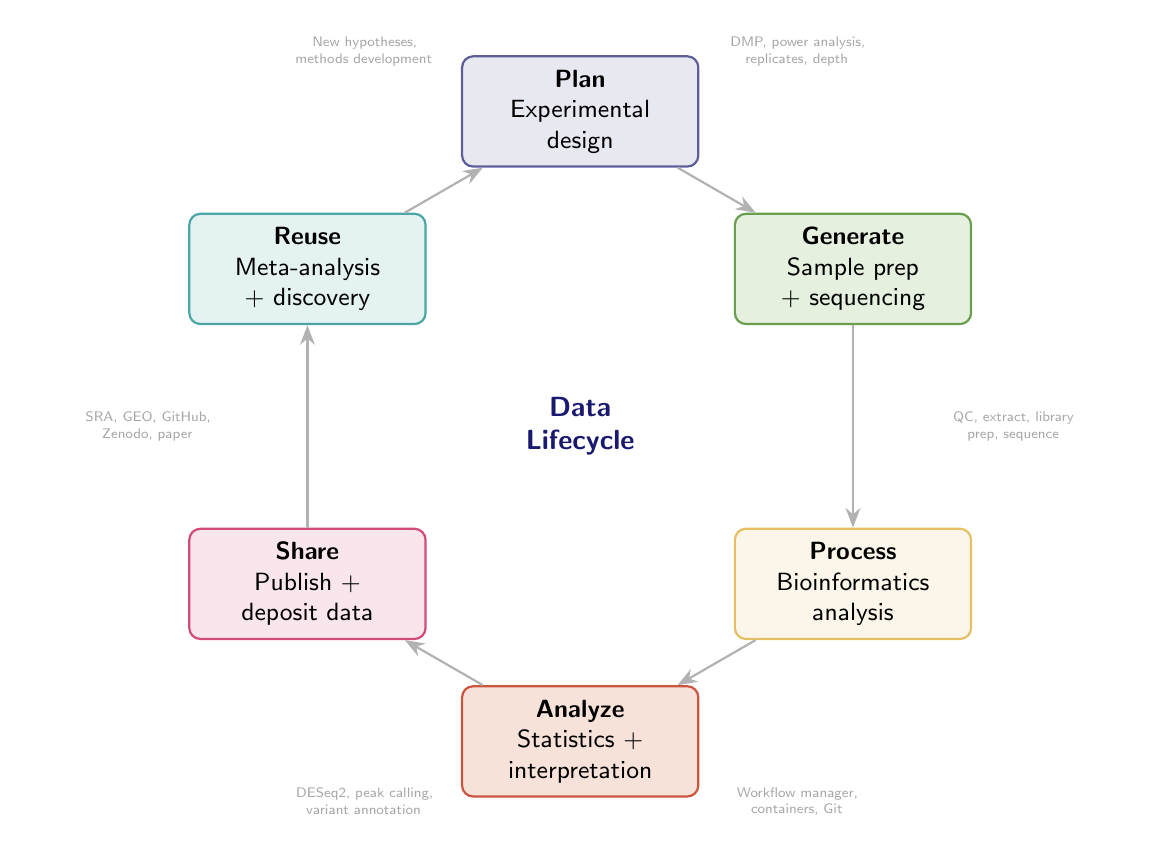
\begin{tikzpicture}[
  phase/.style={
    draw=#1!70, fill=#1!10, rounded corners=4pt,
    minimum width=3cm, minimum height=1.4cm,
    font=\sffamily\small, align=center, thick
  },
  arr/.style={-{Stealth[length=2.5mm]}, thick, gray!60},
  note/.style={font=\tiny\sffamily, text=gray!70, align=center, text width=2.8cm}
]

% Circular layout
\def\R{4.0}
\def\N{6}

\node[phase=MidnightBlue] (plan) at (90:\R) {\textbf{Plan}\\Experimental\\design};
\node[phase=OliveGreen]   (gen)  at (30:\R) {\textbf{Generate}\\Sample prep\\+ sequencing};
\node[phase=Goldenrod]    (proc) at (-30:\R) {\textbf{Process}\\Bioinformatics\\analysis};
\node[phase=BrickRed]     (ana)  at (-90:\R) {\textbf{Analyze}\\Statistics +\\interpretation};
\node[phase=purple]       (share) at (-150:\R) {\textbf{Share}\\Publish +\\deposit data};
\node[phase=teal]         (reuse) at (150:\R) {\textbf{Reuse}\\Meta-analysis\\+ discovery};

% Arrows forming a cycle
\draw[arr] (plan) -- (gen);
\draw[arr] (gen) -- (proc);
\draw[arr] (proc) -- (ana);
\draw[arr] (ana) -- (share);
\draw[arr] (share) -- (reuse);
\draw[arr] (reuse) -- (plan);

% Central label
\node[font=\sffamily\bfseries, text=MidnightBlue, align=center] at (0,0) {Data\\Lifecycle};

% Outer annotations
\node[note] at (60:\R+1.5) {DMP, power analysis,\\replicates, depth};
\node[note] at (0:\R+1.5) {QC, extract, library\\prep, sequence};
\node[note] at (-60:\R+1.5) {Workflow manager,\\containers, Git};
\node[note] at (-120:\R+1.5) {DESeq2, peak calling,\\variant annotation};
\node[note] at (-180:\R+1.5) {SRA, GEO, GitHub,\\Zenodo, paper};
\node[note] at (120:\R+1.5) {New hypotheses,\\methods development};

\end{tikzpicture}
\caption[The NGS data lifecycle.]{The data lifecycle for NGS projects. Data flows from planning through generation, processing, analysis, sharing, and reuse. The cycle is iterative: reuse of public data generates new hypotheses that drive new experiments. Each phase has associated standards, tools, and best practices described throughout this book.}
\label{fig:data-lifecycle}
\end{figure}

%=============================================================================
\section{Practical Data Submission Checklist}
\label{sec:datastandards:checklist}
%=============================================================================

\begin{protocolbox}[title={Pre-Publication Data Submission Checklist}]
Complete these steps before submitting your manuscript:
\begin{enumerate}[itemsep=3pt]
  \item \textbf{Raw data to SRA/ENA:}
  \begin{itemize}[nosep]
    \item Register a BioProject with a descriptive title and abstract.
    \item Create BioSamples with complete metadata (organism, tissue, genotype, condition).
    \item Upload FASTQ files and link to BioSamples.
    \item Set a release date (can be set to future date for embargo until publication).
  \end{itemize}

  \item \textbf{Processed data to GEO:}
  \begin{itemize}[nosep]
    \item Prepare processed files (count matrices, peak BED files, BigWig tracks).
    \item Create a GEO submission with sample-level metadata.
    \item Link to SRA BioProject for raw data.
  \end{itemize}

  \item \textbf{Code to GitHub + Zenodo:}
  \begin{itemize}[nosep]
    \item Push all analysis code (Snakemake/Nextflow workflows, scripts) to GitHub.
    \item Include a README with instructions for reproducing the analysis.
    \item Create a Zenodo release to get a DOI for permanent archival.
    \item Include Conda environment files or Dockerfiles.
  \end{itemize}

  \item \textbf{In the manuscript:}
  \begin{itemize}[nosep]
    \item Report all accession numbers (BioProject, GEO, SRA).
    \item Report all software versions.
    \item Report all key parameters.
    \item Provide the GitHub/Zenodo DOI for analysis code.
  \end{itemize}
\end{enumerate}
\end{protocolbox}

%=============================================================================
\section{Summary}
\label{sec:datastandards:summary}
%=============================================================================

Responsible data management, sharing, and reproducibility practices are not optional extras---they are integral to high-quality genomics research:

\begin{itemize}[itemsep=2pt]
  \item \textbf{Public repositories:} SRA/ENA for raw data, GEO/ArrayExpress for processed data. Data submitted to any INSDC member is automatically shared globally.
  \item \textbf{Consortium portals:} ENCODE, GTEx, TCGA, HCA, and CellxGene provide curated, uniformly processed datasets that serve as community resources.
  \item \textbf{Reference genomes:} Use consistent genome builds and annotations from GENCODE, Ensembl, or RefSeq. Document exact versions.
  \item \textbf{Metadata standards:} MINSEQE defines minimum metadata requirements. Use controlled vocabularies (EFO, CL, OBI) rather than free text.
  \item \textbf{FAIR principles:} Make data Findable (persistent identifiers), Accessible (standard protocols), Interoperable (standard formats), and Reusable (rich metadata and clear licenses).
  \item \textbf{Reproducibility:} Pin software and reference versions, use containers and workflow managers, version-control code with Git, archive on Zenodo for DOIs, and combine code with narrative using literate programming.
  \item \textbf{Data management plans:} Required by most funding agencies. Plan for data generation, storage, sharing, and long-term preservation from the start of the project.
  \item \textbf{Data security:} Human genomic data requires careful attention to consent, de-identification, and controlled access. Follow HIPAA, GDPR, and institutional IRB requirements.
  \item \textbf{Community standards:} ENCODE, IHEC, HCA, and GA4GH establish quality benchmarks and interoperability standards that benefit the entire field.
\end{itemize}

By following these standards and practices, you ensure that your sequencing data contributes not only to your immediate research goals but to the broader scientific community for years to come.


% Part VIII: Democratisation of Sequencing
\part{Democratisation of Sequencing}
\chapter{Accessible Sequencing: Democratising Genomics}
\label{ch:accessible}

\begin{keyconcept}
Sequencing technology is no longer the exclusive province of well-funded core facilities and genome centres. The dramatic reduction in instrument costs, the emergence of portable nanopore sequencers, and the growth of community laboratories have opened genomics to individual researchers, educators, citizen scientists, and field biologists working in remote locations. This chapter maps the landscape of accessible sequencing---from budget planning and platform selection to field deployment, educational applications, and the legal and ethical frameworks that govern this expanding frontier. The goal is to provide a realistic, practical guide for anyone who wants to generate sequence data outside a traditional institutional setting.
\end{keyconcept}

%% ============================================================
\section{The Landscape of Accessible Sequencing}
\label{sec:accessible:landscape}
%% ============================================================

The cost of sequencing a human genome has fallen from approximately \$2.7 billion (the Human Genome Project, completed 2003) to under \$200 for consumables on the latest Illumina platforms. Yet the cost of \emph{entry}---the capital expenditure required to begin generating sequence data independently---remained prohibitively high until the mid-2010s. The introduction of Oxford Nanopore's MinION in 2014 fundamentally changed this equation, creating a category of sequencing devices that cost less than a high-end laptop.

Today, a researcher, educator, or citizen scientist can enter the sequencing space at several cost tiers:

\begin{itemize}[itemsep=2pt]
  \item \textbf{Under \$1,000:} A MinION starter pack provides the sequencing device itself (the MinION Mk1B) plus initial flow cells and reagents. This is sufficient for bacterial genomes, amplicon sequencing, and educational demonstrations.
  \item \textbf{\$1,000--\$5,000:} Adding a Flongle adapter, additional flow cells, a basic \acrshort{PCR} thermocycler, and a used laptop with a GPU enables a modest but capable sequencing programme.
  \item \textbf{\$5,000--\$10,000:} The Illumina iSeq 100 (list price ${\sim}$\$20,000 new, often available refurbished for \$8,000--\$12,000) or the \acrshort{ONT} PromethION P2 Solo (${\sim}$\$9,800) provides substantially higher throughput while remaining within reach of individual laboratories.
  \item \textbf{\$10,000--\$50,000:} Shared-access models with benchtop instruments such as the Illumina MiSeq or NextSeq 550 become feasible for departments, teaching institutions, and community laboratories.
\end{itemize}

\Cref{tab:accessible:platforms} compares the key accessible sequencing platforms available as of 2025.

\begin{table}[htbp]
\centering
\caption[Comparison of accessible sequencing platforms]{Comparison of accessible sequencing platforms. Costs are approximate and represent list prices for the instrument plus a single run of consumables; actual costs vary by region and negotiation.}
\label{tab:accessible:platforms}
\small
\renewcommand{\arraystretch}{1.3}
\begin{tabularx}{\textwidth}{@{}l l c c c c X@{}}
\toprule
\textbf{Platform} & \textbf{Vendor} & \textbf{Output} & \textbf{Read Length} & \textbf{Accuracy} & \textbf{Cost\fmark{a}} & \textbf{Best For} \\
\midrule
MinION Mk1B & \acrshort{ONT} & 50\gigabase & $>$100\kilobase & Q20+ (sup) & \$1,000 & Portability, long reads, rapid prototyping \\
\addlinespace
Flongle & \acrshort{ONT} & 2.8\gigabase & $>$100\kilobase & Q20+ (sup) & \$140/run & Low-cost amplicons, targeted panels, teaching \\
\addlinespace
P2 Solo & \acrshort{ONT} & 290\gigabase & $>$100\kilobase & Q20+ (sup) & \$9,800 & Human \acrshort{WGS}, large genomes, production \\
\addlinespace
iSeq 100 & Illumina & 1.2\gigabase & $2 \times 150\basepair$ & $>$Q30 & \$20,000 & Small panels, 16S, low-throughput short reads \\
\bottomrule
\end{tabularx}
\vspace{2pt}
{\footnotesize \fmark{a} MinION cost reflects the starter pack; Flongle cost is per-flow-cell consumable; P2 Solo and iSeq 100 costs are instrument list prices.}
\end{table}

\begin{tipbox}[title={Refurbished and Decommissioned Instruments}]
Illumina MiSeq and Ion Torrent PGM instruments are increasingly available on the secondary market as institutions upgrade. A refurbished MiSeq can often be obtained for \$15,000--\$25,000---a fraction of its original list price. Ensure that service contracts or at minimum a warranty period are included, and verify that the instrument firmware is compatible with current reagent kits before purchasing.
\end{tipbox}

The choice between platforms involves trade-offs that depend on the application. Short-read platforms (iSeq 100, MiSeq) offer high per-base accuracy and compatibility with the vast existing ecosystem of Illumina-based bioinformatics tools (see \cref{ch:seqprinciples}). Long-read platforms (\acrshort{ONT} MinION, Flongle, P2 Solo) offer portability, real-time data streaming, the ability to detect base modifications natively, and ultra-long reads that simplify de novo assembly (see \cref{ch:longread}).

%% ============================================================
\section{Oxford Nanopore for the Individual Researcher}
\label{sec:accessible:ont}
%% ============================================================

Oxford Nanopore Technologies has done more than any other company to lower the barrier to entry for independent sequencing. The MinION---a USB-powered sequencing device roughly the size of a stapler---was the first sequencing instrument that a single researcher could purchase, unbox, and begin using in an afternoon.

\subsection{MinION and Mk1C}
\label{subsec:accessible:minion}

The \textbf{MinION Mk1B} is the flagship accessible device. It contains no internal compute; sequencing data is streamed via USB~3.0 to a host computer where basecalling is performed. The \textbf{MinION Mk1C} integrates an NVIDIA Jetson Xavier GPU module with a touchscreen, making it a self-contained sequencing-and-basecalling device---particularly useful for field deployment where carrying a separate laptop is impractical.

Key specifications of the MinION platform:

\begin{itemize}[itemsep=2pt]
  \item \textbf{Flow cell:} R10.4.1 (current generation), containing ${\sim}$2,048 individually addressable nanopores arranged in 512 channels.
  \item \textbf{Output:} Up to 50\gigabase{} per flow cell under ideal conditions; typical yields range from 10--30\gigabase{} depending on library quality and pore occupancy.
  \item \textbf{Read length:} Limited primarily by input DNA fragment length, not the device. Reads exceeding 4\megabase{} have been demonstrated.
  \item \textbf{Run time:} Up to 72 hours, but most runs yield the majority of data within 24--48 hours.
  \item \textbf{Accuracy:} With R10.4.1 chemistry and the ``super-accurate'' (sup) basecalling model, simplex read accuracy exceeds Q20 ($>$99\% per-base). Duplex reads (both strands of the same molecule) achieve Q30+ ($>$99.9\%).
  \item \textbf{Power draw:} Approximately 2--3\,W for the MinION device itself; the host computer or Mk1C draws an additional 10--30\,W.
\end{itemize}

\subsection{Flongle: The Disposable Flow Cell}
\label{subsec:accessible:flongle}

The \textbf{Flongle} is a single-use flow cell adapter for the MinION that contains 126 channels (compared to 512 on a standard MinION flow cell). It produces up to 2.8\gigabase{} of data---sufficient for many targeted applications---at a consumable cost of approximately \$140 per flow cell (including the adapter, which is reusable).

The Flongle is ideally suited for:

\begin{itemize}[itemsep=2pt]
  \item Bacterial genome assembly (a 5\megabase{} genome at 30$\times$ coverage requires only 150\megabase{} of data).
  \item Amplicon sequencing (16S, ITS, \acrshort{PCR} products for genotyping).
  \item \acrshort{QC} runs to verify library quality before committing a full MinION flow cell.
  \item Teaching and training exercises.
  \item Rapid pathogen identification in point-of-care settings.
\end{itemize}

The economics of the Flongle are compelling: at \$140 per flow cell, the per-sample cost for a bacterial genome (including library preparation) is approximately \$200--\$250. This is competitive with outsourcing to a core facility, with the added benefit of turnaround times measured in hours rather than weeks.

\subsection{PromethION P2 Solo}
\label{subsec:accessible:p2solo}

For researchers who need higher throughput but cannot justify a full PromethION 48 ($>$\$200,000), the \textbf{PromethION P2 Solo} offers two PromethION flow cells (each with ${\sim}$2,675 channels) in a benchtop format priced at approximately \$9,800. Each P2 Solo flow cell can yield up to 145\gigabase{}, making 30$\times$ human \acrshort{WGS} feasible from a single flow cell.

The P2 Solo requires a dedicated compute resource for basecalling, ideally a workstation equipped with a high-end NVIDIA GPU (see \cref{tab:accessible:basecalling}).

\subsection{Computing Requirements for Nanopore Basecalling}
\label{subsec:accessible:compute}

Basecalling---the process of translating raw electrical signal into nucleotide sequences---is the most computationally intensive step in the \acrshort{ONT} workflow. The basecalling model used dramatically affects both accuracy and compute time. \Cref{tab:accessible:basecalling} provides benchmarks for basecalling a typical MinION run (${\sim}$20\gigabase{}) on different hardware configurations.

\begin{table}[htbp]
\centering
\caption[Basecalling compute benchmarks]{Approximate basecalling times for 20\gigabase{} of MinION R10.4.1 data using \software{Dorado} on different hardware configurations. Times are wall-clock hours for a complete run.}
\label{tab:accessible:basecalling}
\small
\renewcommand{\arraystretch}{1.3}
\begin{tabularx}{\textwidth}{@{}l l c c c@{}}
\toprule
\textbf{Hardware} & \textbf{Specification} & \textbf{Fast} & \textbf{HAC} & \textbf{SUP} \\
\midrule
CPU only & 16-core Xeon / Ryzen 9 & 8\,h & 48\,h & $>$200\,h \\
\addlinespace
Entry GPU & NVIDIA RTX 3060 (12\,GB) & 0.5\,h & 2.5\,h & 12\,h \\
\addlinespace
Mid-range GPU & NVIDIA RTX 4080 (16\,GB) & 0.3\,h & 1.2\,h & 5\,h \\
\addlinespace
High-end GPU & NVIDIA A100 (80\,GB) & 0.2\,h & 0.6\,h & 2\,h \\
\addlinespace
Mk1C (internal) & Jetson Xavier NX & 4\,h & 18\,h & N/A\fmark{b} \\
\addlinespace
Apple Silicon & M2 Pro (16\,GB unified) & 1.5\,h & 6\,h & 28\,h \\
\bottomrule
\end{tabularx}
\vspace{2pt}
{\footnotesize \fmark{b} The Mk1C hardware is insufficient for SUP basecalling in a practical time frame; use an external GPU workstation for SUP accuracy.}
\end{table}

\begin{warningbox}[title={Basecalling Model Selection}]
The choice of basecalling model involves a direct trade-off between accuracy and compute cost. The ``fast'' model (approximately Q8--Q10) is suitable for real-time species identification during a run but insufficient for variant calling. The ``high accuracy'' (HAC, Q15--Q18) model is appropriate for most applications. The ``super-accurate'' (SUP, Q20+) model is recommended for variant calling, methylation detection, and any application where per-base accuracy is critical---but requires a capable GPU. Running SUP basecalling on a CPU is not practical for production use.
\end{warningbox}

\begin{lstlisting}[language=bash,caption={Basecalling with Dorado on a GPU workstation.},label=lst:dorado-basecall]
# Download the appropriate model
dorado download --model dna_r10.4.1_e8.2_400bps_sup@v5.0.0

# Basecall a directory of POD5 files using the SUP model
dorado basecaller \
  dna_r10.4.1_e8.2_400bps_sup@v5.0.0 \
  /data/pod5/ \
  --device cuda:0 \
  --emit-moves \
  > basecalled.bam

# Convert to FASTQ if needed
samtools fastq basecalled.bam > basecalled.fastq

# For methylation-aware basecalling (5mC and 5hmC)
dorado basecaller \
  dna_r10.4.1_e8.2_400bps_sup@v5.0.0 \
  /data/pod5/ \
  --device cuda:0 \
  --modified-bases 5mCG_5hmCG \
  > basecalled_mods.bam
\end{lstlisting}

%% ============================================================
\section{Budget Planning and Cost Modelling}
\label{sec:accessible:budget}
%% ============================================================

One of the most common mistakes made by researchers entering the accessible sequencing space is underestimating total project costs. The sequencing device itself is often the smallest line item; reagents, library preparation kits, sample preparation consumables, compute resources, and personnel time dominate the budget. This section provides itemised cost models for five common project types.

\subsection{Itemised Cost Models}
\label{subsec:accessible:costmodels}

\Cref{tab:accessible:costmodels} provides realistic, itemised cost estimates for five representative projects using \acrshort{ONT} MinION or Flongle as the primary sequencing platform. All costs are approximate and based on 2025 list prices.

\begin{table}[htbp]
\centering
\caption[Itemised cost models for five accessible sequencing projects]{Itemised cost models for five representative projects. Costs assume a MinION Mk1B already in hand (starter pack, \$1,000, not included in per-project costs). Library preparation costs include consumables only.}
\label{tab:accessible:costmodels}
\small
\renewcommand{\arraystretch}{1.25}
\begin{tabularx}{\textwidth}{@{}X r r r r r@{}}
\toprule
\textbf{Cost Item} & \textbf{Bacterial} & \textbf{16S} & \textbf{Human} & \textbf{eDNA} & \textbf{Food} \\
 & \textbf{Genome} & \textbf{Amplicon} & \textbf{WGS} & \textbf{Biodiv.} & \textbf{Auth.} \\
\midrule
DNA extraction kit & \$50 & \$120 & \$30 & \$200 & \$80 \\
Library prep kit & \$120 & \$60 & \$180 & \$90 & \$90 \\
Flow cell (type) & \$140\fmark{c} & \$140\fmark{c} & \$900\fmark{d} & \$140\fmark{c} & \$140\fmark{c} \\
Barcoding expansion & --- & \$45 & --- & \$45 & \$45 \\
\acrshort{PCR} primers / reagents & --- & \$30 & --- & \$30 & \$30 \\
Compute (cloud GPU) & \$5 & \$2 & \$40 & \$5 & \$3 \\
Consumables (tips, tubes) & \$15 & \$25 & \$20 & \$30 & \$20 \\
\midrule
\textbf{Total per project} & \textbf{\$330} & \textbf{\$422} & \textbf{\$1,170} & \textbf{\$540} & \textbf{\$408} \\
\textbf{Samples per run} & 1 & 24 & 1 & 12 & 12 \\
\textbf{Cost per sample} & \textbf{\$330} & \textbf{\$18} & \textbf{\$1,170} & \textbf{\$45} & \textbf{\$34} \\
\bottomrule
\end{tabularx}
\vspace{2pt}
{\footnotesize \fmark{c} Flongle flow cell. \fmark{d} Standard MinION R10.4.1 flow cell.}
\end{table}

\begin{keyconcept}[title={Hidden Costs to Budget For}]
Beyond the obvious consumables, accessible sequencing projects should budget for:
\begin{itemize}[nosep]
  \item \textbf{Sample collection and transport:} Preservation reagents, cold chain, shipping.
  \item \textbf{Data storage:} A single MinION run generates 50--200\,GB of raw POD5 files. Cloud storage costs accumulate.
  \item \textbf{Compute:} GPU basecalling, alignment, assembly. Cloud GPU instances (e.g., AWS \texttt{g5.xlarge}) cost \$1--\$3/hour.
  \item \textbf{Failed runs:} Budget for a 10--20\% failure rate due to clogged pores, degraded reagents, or library preparation issues.
  \item \textbf{Personnel time:} Even ``automated'' protocols require skilled hands. Factor in training time.
\end{itemize}
\end{keyconcept}

\subsection{Reagent Shelf Life}
\label{subsec:accessible:shelflife}

Reagent degradation is a frequently overlooked cost driver, particularly for low-throughput users who may not consume reagents before expiration. Key shelf-life considerations include:

\begin{itemize}[itemsep=2pt]
  \item \textbf{\acrshort{ONT} flow cells:} Stored at 2--8$^{\circ}$C, flow cells have a shelf life of approximately 8--12 weeks from manufacture. Using flow cells near their expiration date results in reduced pore counts and lower yields. Order flow cells as close to the planned experiment date as possible.
  \item \textbf{Library preparation kits:} Most \acrshort{ONT} library prep kits (Ligation Sequencing Kit, Rapid Barcoding Kit) have a shelf life of 3--6 months at $-20^{\circ}$C. Kits contain enzymes that degrade with repeated freeze--thaw cycles; aliquot on first use.
  \item \textbf{DNA extraction reagents:} Column-based kits (Qiagen, Zymo) are stable for 12--18 months at room temperature. Enzymatic lysis reagents may have shorter shelf lives.
  \item \textbf{\acrshort{PCR} reagents:} Polymerases and master mixes are typically stable for 6--12 months at $-20^{\circ}$C. Primers dissolved in TE buffer are stable for years at $-20^{\circ}$C.
\end{itemize}

\begin{tipbox}[title={Group Purchasing for Low-Throughput Users}]
If you sequence infrequently (fewer than one run per month), consider coordinating with nearby laboratories or community lab members to place joint orders, share flow cells, and run samples together. A Flongle flow cell with native barcoding can accommodate up to 24 samples---pooling samples from multiple users minimises per-sample cost and reduces reagent waste.
\end{tipbox}

\subsection{Shared Equipment Models and Cost-per-Sample Analysis}
\label{subsec:accessible:shared}

For institutions considering a shared sequencing resource, the cost per sample can be modelled as:

\begin{equation}
\label{eq:accessible:costsample}
C_{\text{sample}} = \frac{C_{\text{instrument}}}{N_{\text{lifetime}} \times S_{\text{run}}} + \frac{C_{\text{consumable}}}{S_{\text{run}}} + C_{\text{extraction}} + C_{\text{overhead}}
\end{equation}

\noindent where $C_{\text{instrument}}$ is the capital cost of the instrument, $N_{\text{lifetime}}$ is the total number of runs over the instrument's lifetime, $S_{\text{run}}$ is the number of samples per run, $C_{\text{consumable}}$ is the per-run consumable cost (flow cell + library prep), $C_{\text{extraction}}$ is the per-sample DNA extraction cost, and $C_{\text{overhead}}$ captures personnel time, compute, storage, and facility costs.

For example, consider a community laboratory that purchases a MinION starter pack (\$1,000) and plans to perform 100 Flongle runs over two years, with 12 barcoded samples per run:

\begin{align}
C_{\text{sample}} &= \frac{\$1{,}000}{100 \times 12} + \frac{\$140 + \$90}{12} + \$10 + \$5 \notag \\
                    &= \$0.83 + \$19.17 + \$10 + \$5 \notag \\
                    &= \$35.00 \text{ per sample}
\end{align}

This is competitive with commercial sequencing services, with the added advantages of rapid turnaround (same-day results), complete control over the protocol, and the educational value of performing sequencing in-house.

%% ============================================================
\section{Community Labs and Maker Spaces}
\label{sec:accessible:community}
%% ============================================================

Community biology laboratories---also known as biohacker spaces or DIY biology labs---have emerged as important venues for accessible sequencing. These spaces provide shared equipment, training, and a collaborative community that lowers the barrier to entry for individuals who lack institutional affiliation.

\subsection{Prominent Community Laboratories}
\label{subsec:accessible:communitylabs}

Several community labs have pioneered accessible sequencing programmes:

\begin{description}[style=nextline, font=\bfseries, itemsep=4pt]
  \item[Genspace (New York City, USA)]
  Founded in 2010, Genspace is one of the world's first community biology laboratories. It offers courses in DNA extraction, \acrshort{PCR}, gel electrophoresis, and nanopore sequencing. Genspace operates as a non-profit with membership fees (\$100/month) and course-based revenue. The lab maintains MinION devices available for member use and has contributed to citizen science projects including environmental DNA monitoring of the Gowanus Canal.

  \item[BioCurious (Santa Clara, California, USA)]
  A community laboratory in Silicon Valley that has hosted sequencing workshops and synthetic biology projects since 2011. BioCurious provides a BSL-1 workspace, shared equipment, and mentorship from experienced molecular biologists.

  \item[La Paillasse (Paris, France)]
  One of Europe's leading community biology spaces, La Paillasse has been involved in open-source biology projects since 2014. It has hosted nanopore sequencing workshops and contributed to food safety and environmental monitoring projects.

  \item[BioFoundry (Sydney, Australia)]
  Australia's first community laboratory, BioFoundry offers nanopore sequencing training and has supported eDNA biodiversity monitoring projects in urban waterways.
\end{description}

\subsection{Setting Up a Sequencing Corner}
\label{subsec:accessible:setup}

A functional sequencing workspace can be established within a community laboratory, teaching institution, or even a well-organised home laboratory, provided that appropriate biosafety measures are in place. The following requirements apply to \textbf{BSL-1} (Biosafety Level 1) work only---that is, work with organisms and samples that pose no known risk to healthy adults.

\begin{protocolbox}[title={Minimum Requirements for a BSL-1 Sequencing Workspace}]
\begin{enumerate}[itemsep=2pt]
  \item \textbf{Work surface:} A cleanable, non-porous bench surface (stainless steel, epoxy resin, or chemical-resistant laminate). Minimum 1.5\,m $\times$ 0.6\,m of clear bench space.
  \item \textbf{Decontamination:} 10\% bleach solution or 70\% ethanol for surface decontamination. An autoclave or pressure cooker for waste decontamination.
  \item \textbf{Personal protective equipment (PPE):} Disposable nitrile gloves, laboratory coat, and safety glasses.
  \item \textbf{Waste disposal:} Biohazard bags for contaminated consumables; sharps container if using scalpels or needles.
  \item \textbf{Hand washing:} A sink with soap and water within the workspace.
  \item \textbf{No food or drink:} The workspace must be separated from food preparation and consumption areas.
  \item \textbf{Ventilation:} Adequate general ventilation. A biosafety cabinet is \emph{not} required for BSL-1 work but is recommended for handling samples that may contain allergens or irritants.
  \item \textbf{Documentation:} A laboratory notebook (physical or electronic) for recording all procedures, reagent lot numbers, and results.
  \item \textbf{Training:} All users should receive basic laboratory safety training covering chemical hazards, biological waste handling, and emergency procedures.
\end{enumerate}
\end{protocolbox}

\subsection{Minimum Equipment for a Sequencing Laboratory}
\label{subsec:accessible:equipment}

\Cref{tab:accessible:equipment} lists the minimum equipment required for a functional nanopore sequencing laboratory, along with approximate costs and potential budget alternatives.

\begin{table}[htbp]
\centering
\caption[Minimum equipment for a nanopore sequencing laboratory]{Minimum equipment for a basic nanopore sequencing laboratory. ``Budget alternative'' indicates lower-cost substitutes suitable for educational or low-throughput settings.}
\label{tab:accessible:equipment}
\small
\renewcommand{\arraystretch}{1.3}
\begin{tabularx}{\textwidth}{@{}l r l X@{}}
\toprule
\textbf{Equipment} & \textbf{Cost} & \textbf{Essential?} & \textbf{Budget Alternative} \\
\midrule
MinION Mk1B & \$1,000 & Yes & --- \\
Laptop (16\,GB RAM, GPU) & \$1,200 & Yes & Used/refurbished; cloud basecalling \\
Micropipettes (P2, P20, P200, P1000) & \$1,500 & Yes & Used pipettes (\$200--\$500) \\
Minicentrifuge & \$200 & Yes & --- \\
Vortex mixer & \$150 & Yes & Manual flicking (not recommended) \\
Heat block or thermocycler & \$300 & Yes & Sous vide cooker for lysis steps \\
Magnetic rack (for SPRI beads) & \$50 & Yes & 3D-printed rack with neodymium magnets \\
Qubit fluorometer & \$3,000 & Recommended & NanoDrop (\$1,500) or gel estimation \\
Gel electrophoresis system & \$500 & Recommended & Pre-cast gel kits (\$100) \\
Mini \acrshort{PCR} thermocycler & \$500 & For amplicons & miniPCR (\$500, educational pricing) \\
$-20^{\circ}$C freezer & \$500 & Yes & Shared freezer; dorm-style mini-freezer \\
\midrule
\textbf{Total (essential only)} & \textbf{\$4,900} & & \\
\textbf{Total (with recommended)} & \textbf{\$9,100} & & \\
\bottomrule
\end{tabularx}
\end{table}

\begin{tipbox}[title={3D-Printed and Open-Source Lab Equipment}]
The open-source hardware movement has produced functional designs for many common laboratory instruments. Magnetic racks, tube holders, gel electrophoresis chambers, and even centrifuges can be 3D-printed at a fraction of commercial cost. Resources such as the Open Bioeconomy Lab, NIH 3D Print Exchange, and Thingiverse host verified designs. The \software{OpenPCR} project provides plans for a thermocycler that can be assembled for under \$500.
\end{tipbox}

%% ============================================================
\section{Field Sequencing}
\label{sec:accessible:field}
%% ============================================================

One of the most transformative aspects of portable sequencing is the ability to generate sequence data in the field---at the point of sample collection, in remote locations without reliable electricity or internet, and in outbreak settings where rapid pathogen identification saves lives. The MinION's small size, low power consumption, and tolerance of temperature variation make it uniquely suited to field deployment.

\subsection{Power Requirements}
\label{subsec:accessible:power}

The MinION Mk1B draws approximately 2--3\,W via USB, while the host laptop typically requires 30--65\,W depending on whether GPU basecalling is performed. Total system power for a MinION + laptop configuration is therefore 35--70\,W.

\begin{itemize}[itemsep=2pt]
  \item \textbf{USB power banks:} A 100\,Wh USB-C PD power bank can sustain a MinION + efficient laptop for approximately 2--3 hours of sequencing. Multiple power banks can be carried for extended field work.
  \item \textbf{Solar panels:} A 100\,W portable solar panel with a LiFePO$_4$ battery station (e.g., 500\,Wh capacity) can sustain continuous sequencing during daylight hours and provide 7--10 hours of overnight operation.
  \item \textbf{Vehicle power:} A car cigarette lighter or 12\,V outlet with an inverter provides reliable power for roadside or vehicle-based sequencing.
  \item \textbf{Generator:} For multi-day field campaigns, a small ($<$1\,kW) inverter generator provides indefinite runtime.
\end{itemize}

\subsection{Temperature Constraints}
\label{subsec:accessible:temperature}

\acrshort{ONT} flow cells are sensitive to temperature. The recommended operating range is 20--35$^{\circ}$C; the optimal range is 22--30$^{\circ}$C. Outside this range:

\begin{itemize}[itemsep=2pt]
  \item \textbf{Below 15$^{\circ}$C:} Enzyme activity decreases, translocation speed slows, and basecalling accuracy degrades. In cold environments, insulate the MinION in a small cooler with a chemical hand warmer.
  \item \textbf{Above 35$^{\circ}$C:} Pore lifetime decreases and DNA may denature. In hot environments, shade the device and use a small USB fan for convective cooling. Avoid direct sunlight.
\end{itemize}

\subsection{Data Transfer in the Field}
\label{subsec:accessible:datatransfer}

A single MinION run generates 50--200\,GB of raw signal data (POD5 format). Transferring this volume of data over satellite or cellular networks is often impractical. Strategies include:

\begin{itemize}[itemsep=2pt]
  \item \textbf{On-device basecalling:} Perform basecalling locally (fast or HAC model) to reduce data to 1--5\,GB of FASTQ/BAM, which is transferable over a cellular connection.
  \item \textbf{Real-time selective sequencing:} Use \software{ReadFish} or \acrshort{ONT}'s adaptive sampling to reject off-target reads, reducing data volume and focusing on sequences of interest.
  \item \textbf{Portable storage:} Carry ruggedised external SSDs (2--4\,TB) and transfer data physically when returning from the field.
  \item \textbf{Satellite internet:} Starlink terminals (${\sim}$100\,Mbps) can enable data transfer in remote locations with clear sky access.
\end{itemize}

\subsection{Case Studies in Field Sequencing}
\label{subsec:accessible:fieldcases}

\subsubsection{Real-Time Genomic Surveillance of Ebola (2015)}

The seminal demonstration of field sequencing was performed by Quick et al.\ (2016) during the West African Ebola outbreak. Using MinION devices deployed to Guinea, the team sequenced 142 Ebola virus genomes within 48 hours of sample collection. Real-time phylogenetic analysis revealed transmission chains, identified cross-border transmission events, and demonstrated that the outbreak was sustained by human-to-human transmission rather than repeated zoonotic introductions. The entire sequencing laboratory fit in a single suitcase, operated on a generator, and demonstrated that genomic surveillance could be performed in resource-limited settings with minimal infrastructure.

\subsubsection{eDNA Biodiversity Monitoring}

Environmental DNA (eDNA) is DNA shed by organisms into their environment---water, soil, air---and can be collected non-invasively to survey biodiversity. Portable sequencing brings the analysis to the field site, enabling same-day species detection. Notable deployments include:

\begin{itemize}[itemsep=2pt]
  \item Detection of aquatic species in Amazonian rivers using water samples filtered and sequenced on-site with MinION.
  \item Monitoring of invasive species in the Great Lakes using portable eDNA sequencing at boat launches.
  \item Marine biodiversity surveys at remote coral reef sites, where MinION sequencing of the mitochondrial \gene{COI} barcode region identified fish species present in water samples within hours of collection.
\end{itemize}

These applications are discussed further in the context of metagenomic methods in \cref{ch:metagenomics}.

\subsection{Field Sequencing Setup}
\label{subsec:accessible:fieldsetup}

\Cref{fig:accessible:fieldsetup} illustrates a minimal field sequencing setup. The key principle is to minimise the number of components while maintaining a complete workflow from sample to sequence.

\begin{figure}[htbp]
\centering
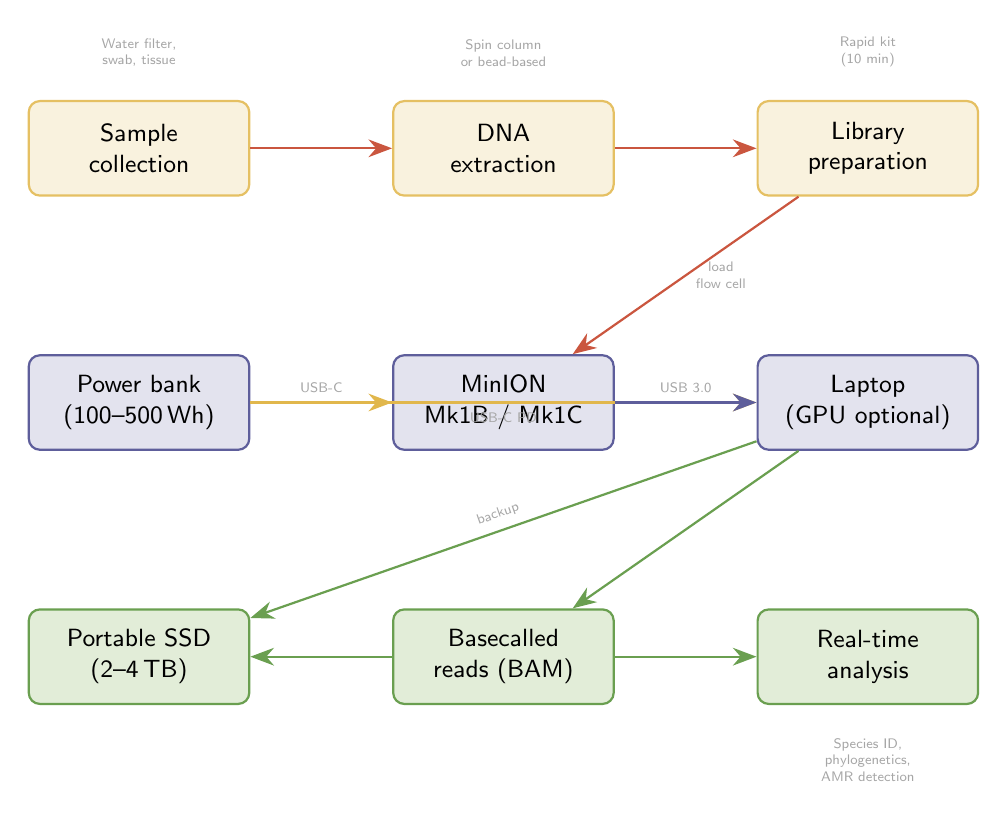
\begin{tikzpicture}[
  >={Stealth[length=3mm]},
  node distance=1.8cm,
  every node/.style={font=\sffamily\small},
  box/.style={
    draw, rounded corners=4pt, minimum width=2.8cm, minimum height=1.2cm,
    align=center, thick
  },
  supply/.style={box, fill=Goldenrod!15, draw=Goldenrod!70},
  device/.style={box, fill=MidnightBlue!12, draw=MidnightBlue!70},
  data/.style={box, fill=OliveGreen!12, draw=OliveGreen!70},
  annotation/.style={font=\sffamily\tiny, text=gray!70, align=center}
]

% --- Row 1: Sample and reagents ---
\node[supply] (sample) {Sample\\collection};
\node[supply, right=of sample] (extraction) {DNA\\extraction};
\node[supply, right=of extraction] (libprep) {Library\\preparation};

% --- Row 2: Sequencing hardware ---
\node[device, below=2.0cm of sample] (power) {Power bank\\(100--500\,Wh)};
\node[device, below=2.0cm of extraction] (minion) {MinION\\Mk1B / Mk1C};
\node[device, below=2.0cm of libprep] (laptop) {Laptop\\(GPU optional)};

% --- Row 3: Data outputs ---
\node[data, below=2.0cm of power] (storage) {Portable SSD\\(2--4\,TB)};
\node[data, below=2.0cm of minion] (basecall) {Basecalled\\reads (BAM)};
\node[data, below=2.0cm of laptop] (analysis) {Real-time\\analysis};

% --- Arrows: sample flow ---
\draw[->, thick, BrickRed!70] (sample) -- (extraction);
\draw[->, thick, BrickRed!70] (extraction) -- (libprep);
\draw[->, thick, BrickRed!70] (libprep) -- (minion) node[midway, right, annotation] {load\\flow cell};

% --- Arrows: power ---
\draw[->, thick, Goldenrod!80] (power) -- (minion) node[midway, above, annotation] {USB-C};
\draw[->, thick, Goldenrod!80] (power) -- (laptop) node[midway, below, annotation, sloped] {USB-C PD};

% --- Arrows: data flow ---
\draw[->, thick, MidnightBlue!70] (minion) -- (laptop) node[midway, above, annotation] {USB 3.0};
\draw[->, thick, OliveGreen!70] (laptop) -- (basecall);
\draw[->, thick, OliveGreen!70] (basecall) -- (analysis);
\draw[->, thick, OliveGreen!70] (laptop) -- (storage) node[midway, above, annotation, sloped] {backup};
\draw[->, thick, OliveGreen!70] (basecall) -- (storage);

% --- Annotations ---
\node[annotation, above=0.3cm of sample] {Water filter,\\swab, tissue};
\node[annotation, above=0.3cm of extraction] {Spin column\\or bead-based};
\node[annotation, above=0.3cm of libprep] {Rapid kit\\(10 min)};
\node[annotation, below=0.3cm of analysis] {Species ID,\\phylogenetics,\\AMR detection};

\end{tikzpicture}
\caption[Field sequencing setup]{Schematic of a minimal field sequencing setup showing the three phases of the workflow: sample preparation (top, gold), sequencing hardware (middle, blue), and data handling (bottom, green). Arrows indicate sample flow (red), power delivery (gold), and data flow (blue/green).}
\label{fig:accessible:fieldsetup}
\end{figure}

\begin{protocolbox}[title={Field Sequencing Packing Checklist}]
The following items constitute a complete field sequencing kit that fits in a single carry-on-sized case:
\begin{enumerate}[itemsep=1pt]
  \item MinION Mk1B (or Mk1C) with USB cable
  \item 2--4 Flongle or MinION flow cells (in cold pack pouch, 2--8$^{\circ}$C)
  \item Rapid Barcoding Kit (SQK-RBK114.24)
  \item Spin-column DNA extraction kit (e.g., Qiagen DNeasy or Zymo Quick-DNA)
  \item Micropipettes (P20, P200) with filter tips
  \item Magnetic rack and AMPure XP beads (or Zymo Select-a-Size)
  \item Minicentrifuge (palm-sized, battery-operated)
  \item Laptop with \software{MinKNOW} and \software{Dorado} pre-installed
  \item 100\,Wh USB-C PD power bank (for MinION) + laptop charger
  \item Portable SSD for data backup
  \item Nitrile gloves, 70\% isopropanol wipes, waste bag
  \item Laboratory notebook and permanent marker
\end{enumerate}
Total weight: approximately 5--7\,kg including the laptop.
\end{protocolbox}

%% ============================================================
\section{Educational and Outreach Applications}
\label{sec:accessible:education}
%% ============================================================

Sequencing technology is an extraordinarily powerful tool for science education. The ability to extract DNA from an organism, generate a sequence, and identify it computationally provides a visceral, end-to-end experience of molecular biology that textbooks alone cannot replicate. The accessibility of nanopore sequencing has made it feasible to bring real sequencing into undergraduate laboratories, high school classrooms, and public outreach events.

\subsection{Designing a Teaching Laboratory Sequencing Module}
\label{subsec:accessible:teachlab}

A successful teaching laboratory sequencing module must be:

\begin{itemize}[itemsep=2pt]
  \item \textbf{Robust:} Protocols must work reliably in the hands of novices. Use the simplest possible library preparation kit (e.g., \acrshort{ONT} Rapid Barcoding Kit, which requires 10 minutes of hands-on time and no \acrshort{PCR}).
  \item \textbf{Fast:} Students must see results within a single laboratory session (3--4 hours). Nanopore sequencing produces data in real time, allowing species identification within 30--60 minutes of loading.
  \item \textbf{Affordable:} Per-student costs must be manageable within institutional teaching budgets.
  \item \textbf{Safe:} All work must be BSL-1 compatible. Use non-pathogenic organisms or environmental samples that pose no known health risk.
  \item \textbf{Pedagogically meaningful:} The experiment should connect to core concepts in molecular biology, genetics, and bioinformatics as covered in the foundational chapters of this book (see \cref{ch:seqprinciples}).
\end{itemize}

\subsection{Suggested Curriculum Outline}
\label{subsec:accessible:curriculum}

The following five-session curriculum is designed for an undergraduate molecular biology or genomics course. Each session is 3--4 hours.

\begin{description}[style=nextline, font=\bfseries, itemsep=4pt]
  \item[Session 1: DNA Extraction and Quantification]
  Students extract DNA from an assigned sample (environmental water, soil, cheek swab, food product, or bacterial culture). They quantify DNA using a Qubit fluorometer and assess quality by gel electrophoresis or NanoDrop A260/A280 ratio. \emph{Learning objectives:} Cell lysis mechanisms, DNA purification chemistry, quality metrics.

  \item[Session 2: Library Preparation and Sequencing]
  Students prepare a nanopore library using the Rapid Barcoding Kit. Each student receives a unique barcode. Barcoded libraries are pooled and loaded onto a single Flongle or MinION flow cell. Sequencing begins during the session and runs overnight. \emph{Learning objectives:} Library preparation principles (see \cref{ch:libprep}), adapter ligation, multiplexing by barcoding.

  \item[Session 3: Basecalling and Quality Control]
  Students retrieve basecalled FASTQ data and perform \acrshort{QC} using \software{NanoPlot} and \software{FastQC}. They examine read length distributions, quality scores, and per-barcode yields. \emph{Learning objectives:} Phred quality scores, read length distributions, demultiplexing.

  \item[Session 4: Bioinformatics Analysis]
  Depending on the sample type: (a) for amplicon data, students run \software{BLAST} or \software{minimap2} against reference databases for species identification; (b) for bacterial genomes, students perform de novo assembly with \software{Flye} and assess assembly quality with \software{QUAST}. \emph{Learning objectives:} Sequence alignment, de novo assembly, genome annotation.

  \item[Session 5: Interpretation and Presentation]
  Students interpret their results in biological context, write a short report, and present findings to the class. For eDNA projects, this may include comparing detected species to known local biodiversity. \emph{Learning objectives:} Scientific communication, critical evaluation of sequence data.
\end{description}

\subsection{Cost Per Student}
\label{subsec:accessible:coststudent}

Assuming a class of 24 students sharing a single Flongle flow cell with barcoding:

\begin{align}
C_{\text{student}} &= \frac{C_{\text{flowcell}} + C_{\text{libprep}} + C_{\text{barcoding}}}{24} + C_{\text{extraction}} + C_{\text{consumables}} \notag \\
                     &= \frac{\$140 + \$60 + \$45}{24} + \$8 + \$5 \notag \\
                     &= \$10.21 + \$8 + \$5 \notag \\
                     &= \$23.21 \text{ per student}
\end{align}

This is comparable to the cost of a conventional molecular biology teaching lab exercise involving \acrshort{PCR} and gel electrophoresis, and far less expensive than outsourcing Sanger sequencing of individual student samples.

\begin{tipbox}[title={Oxford Nanopore Educational Discounts}]
\acrshort{ONT} offers an educational programme with discounted starter packs and flow cells for registered academic institutions. Contact the \acrshort{ONT} education team or check the Oxford Nanopore store for current academic pricing. Several grant programmes (e.g., the HHMI Inclusive Excellence programme in the US, the Wellcome Trust Public Engagement Grants in the UK) specifically fund sequencing equipment for teaching laboratories.
\end{tipbox}

\subsection{High School Protocols}
\label{subsec:accessible:highschool}

Sequencing can be brought into high school settings with appropriate simplification:

\begin{itemize}[itemsep=2pt]
  \item \textbf{Pre-extracted DNA:} Provide students with pre-extracted, quantified DNA to avoid the time and consumable cost of extraction in a high school setting.
  \item \textbf{Teacher-performed library preparation:} The teacher or a trained assistant prepares the library. Students participate in loading the flow cell and monitoring the sequencing run.
  \item \textbf{Simplified bioinformatics:} Use \software{EPI2ME} (Oxford Nanopore's cloud-based analysis platform) or pre-built \software{Galaxy} workflows rather than command-line tools.
  \item \textbf{Focus on species identification:} The ``What's in my sample?'' question (species identification from environmental DNA, food products, or bacterial cultures) is inherently engaging and requires minimal bioinformatics infrastructure.
  \item \textbf{Partner with a local university:} University researchers can provide equipment, expertise, and mentorship. Many universities have outreach programmes that actively seek partnerships with local schools.
\end{itemize}

%% ============================================================
\section{What Can You Realistically Do with \$1,000?}
\label{sec:accessible:thousand}
%% ============================================================

The MinION starter pack costs approximately \$1,000 and includes the device, two Flongle flow cells, one MinION flow cell, and a wash kit. With this initial investment, what sequencing projects are realistically achievable? \Cref{tab:accessible:feasibility} provides a feasibility matrix.

\begin{table}[htbp]
\centering
\caption[Feasibility matrix: what \$1,000 can accomplish]{Feasibility matrix for sequencing projects within a \$1,000 total budget (including the MinION starter pack). Coverage is estimated for the included flow cells. ``Feasible'' indicates that useful results can be obtained; ``marginal'' indicates that results are possible but may be incomplete.}
\label{tab:accessible:feasibility}
\small
\renewcommand{\arraystretch}{1.3}
\begin{tabularx}{\textwidth}{@{}X c c c l@{}}
\toprule
\textbf{Project} & \textbf{Genome Size} & \textbf{Data Needed} & \textbf{Achievable?} & \textbf{Notes} \\
\midrule
Bacterial genome (single) & 5\megabase & 150\megabase{} (30$\times$) & Feasible & Flongle; excellent results \\
\addlinespace
16S amplicon (24 samples) & N/A & 50\megabase & Feasible & Flongle + barcoding \\
\addlinespace
Fungal genome & 30--40\megabase & 1.2\gigabase{} (30$\times$) & Feasible & Flongle; sufficient yield \\
\addlinespace
Plant/insect genome & 200\megabase--2\gigabase & 6--60\gigabase{} (30$\times$) & Marginal & MinION flow cell; low coverage for large genomes \\
\addlinespace
Human \acrshort{WGS} (30$\times$) & 3.1\gigabase & 93\gigabase & Not feasible & Requires multiple flow cells (\$900+ each) \\
\addlinespace
Viral genome & 10--30\kilobase & $<$1\megabase & Feasible & Flongle; massive over-coverage \\
\addlinespace
eDNA species detection & N/A & 100\megabase & Feasible & Flongle; amplicon approach \\
\addlinespace
Food authentication & N/A & 100\megabase & Feasible & Flongle; barcode approach \\
\bottomrule
\end{tabularx}
\end{table}

\begin{warningbox}[title={Honest Expectations}]
The \$1,000 entry point is real but comes with important caveats:
\begin{itemize}[nosep]
  \item The starter pack does \emph{not} include DNA extraction kits, library preparation reagents, pipettes, or any other laboratory equipment. Total out-of-pocket cost for a first project is realistically \$1,300--\$1,800.
  \item The included flow cells have limited shelf life. If you do not use them within 8--12 weeks, pore counts degrade significantly.
  \item Basecalling at SUP accuracy requires a computer with a capable GPU (\$800+ if purchased new) or access to cloud computing.
  \item Nanopore sequencing has a steeper learning curve than users accustomed to ``send sample, receive data'' core facility models. Expect your first 2--3 runs to be practice runs with suboptimal results.
  \item Assembly, annotation, and downstream analysis require bioinformatics skills. Free resources (e.g., \software{Galaxy}, \acrshort{ONT}'s \software{EPI2ME}, this textbook) can help, but plan for a learning investment.
\end{itemize}
\end{warningbox}

\begin{tipbox}[title={Maximising the Value of Your First Flow Cell}]
Your first MinION or Flongle run should be a low-stakes experiment designed to familiarise you with the workflow. Suggestions:
\begin{itemize}[nosep]
  \item Extract DNA from an easily lysed bacterium (e.g., \species{Escherichia coli} DH5$\alpha$) and prepare a rapid library. The genome is well-characterised, so you can assess your results against the known reference.
  \item Use the \acrshort{ONT} Lambda phage control DNA included in many kits as a positive control alongside your experimental sample.
  \item Do not attempt barcoding on your first run---run a single unbarcoded library to simplify troubleshooting.
\end{itemize}
\end{tipbox}

%% ============================================================
\section{Citizen Science Sequencing Projects}
\label{sec:accessible:citizenscience}
%% ============================================================

The accessibility of nanopore sequencing has enabled a new category of citizen science: projects in which non-professional scientists generate and analyse sequence data to address questions of community relevance. Unlike traditional citizen science (which typically involves observation and data collection), sequencing-based citizen science produces molecular data that can contribute to professional research.

\subsection{Environmental DNA Barcoding}
\label{subsec:accessible:edna}

Environmental DNA (eDNA) barcoding is perhaps the most natural fit for citizen science sequencing. Participants collect water, soil, or air samples from their local environment, extract DNA, amplify taxonomic barcode regions (mitochondrial \gene{COI} for animals, \gene{rbcL}/\gene{matK} for plants, 16S for bacteria, ITS for fungi), and sequence the amplicons on a MinION or Flongle.

A well-designed eDNA citizen science project includes:

\begin{enumerate}[itemsep=2pt]
  \item \textbf{Standardised sampling protocol:} Define sample volume, filtration method, preservation buffer, and collection metadata (GPS coordinates, date, water temperature, pH).
  \item \textbf{Centralised library preparation:} Participants send extracted DNA (or even raw samples with preservation buffer) to a central laboratory for library preparation and sequencing. This ensures consistent quality.
  \item \textbf{Open data portal:} Results are uploaded to a public database where participants and the broader community can explore detected species, visualise biodiversity maps, and track changes over time.
  \item \textbf{Quality assurance:} Include negative controls (blank extractions, no-template \acrshort{PCR} controls) and positive controls (spike-in of known DNA) in every batch.
\end{enumerate}

\subsection{Food Fraud Detection}
\label{subsec:accessible:foodfraud}

Food fraud---the deliberate mislabelling or adulteration of food products---is a global problem affecting seafood, meat, spices, olive oil, and honey. DNA barcoding can detect species substitution (e.g., tilapia sold as red snapper) with high sensitivity and specificity.

Citizen science food authentication projects have been conducted by community laboratories, journalism organisations, and consumer advocacy groups. A typical workflow involves:

\begin{itemize}[itemsep=2pt]
  \item Purchasing food products from local markets and supermarkets.
  \item Extracting DNA using commercial kits optimised for processed food matrices.
  \item Amplifying species-specific markers (\gene{COI}, \gene{cytb}, 16S) with universal or taxon-specific primers.
  \item Sequencing amplicons on a Flongle and querying results against BOLD (Barcode of Life Data System) or NCBI \software{BLAST}.
\end{itemize}

\begin{keyconcept}[title={DNA Barcoding for Species Identification}]
DNA barcoding uses a short, standardised gene region to identify the species of origin of a biological sample. The most commonly used barcode regions are:
\begin{description}[nosep]
  \item[\gene{COI}] Cytochrome c oxidase subunit I (${\sim}$658\basepair). The standard barcode for animals. Deposited in the BOLD database ($>$14 million records).
  \item[\gene{rbcL}] RuBisCO large subunit. A standard plant barcode.
  \item[\gene{matK}] Maturase K. Used in combination with \gene{rbcL} for plants.
  \item[ITS] Internal transcribed spacer of ribosomal DNA. The standard fungal barcode.
  \item[16S rRNA] Used for bacterial and archaeal identification (see \cref{ch:metagenomics}).
\end{description}
\end{keyconcept}

\subsection{Antimicrobial Resistance Monitoring in Waterways}
\label{subsec:accessible:amr}

Antimicrobial resistance (\acrshort{AMR}) genes in environmental water are a growing public health concern. Rivers, lakes, and wastewater effluent harbour bacteria carrying resistance genes that can transfer to human pathogens. Citizen science monitoring of \acrshort{AMR} in local waterways can:

\begin{itemize}[itemsep=2pt]
  \item Establish baseline levels of resistance genes in local water bodies.
  \item Detect hotspots near hospitals, farms, and wastewater treatment plants.
  \item Track seasonal and temporal trends.
  \item Generate data that informs public health policy.
\end{itemize}

A nanopore-based \acrshort{AMR} monitoring workflow involves collecting water samples, extracting metagenomic DNA, performing either shotgun sequencing or targeted amplification of known resistance genes, and querying results against the CARD (Comprehensive Antibiotic Resistance Database) or ResFinder databases.

\begin{lstlisting}[language=bash,caption={AMR gene detection from environmental water using nanopore data.},label=lst:amr-detection]
# Basecall raw data
dorado basecaller \
  dna_r10.4.1_e8.2_400bps_hac@v5.0.0 \
  /data/pod5/ --device cuda:0 > reads.bam

# Convert to FASTQ
samtools fastq reads.bam > reads.fastq

# Map reads against CARD database
minimap2 -a card_database.fasta reads.fastq | \
  samtools sort -o aligned_card.bam
samtools index aligned_card.bam

# Alternatively, use ABRicate for rapid AMR screening
abricate --db card reads.fasta > amr_results.tab
abricate --summary amr_results.tab > amr_summary.tab

# Visualise results
cat amr_summary.tab | column -t
\end{lstlisting}

\subsection{Concrete Project Examples}
\label{subsec:accessible:projectexamples}

\Cref{tab:accessible:citizenprojects} summarises several concrete citizen science sequencing projects that have been successfully conducted or are currently active.

\begin{table}[htbp]
\centering
\caption[Citizen science sequencing project examples]{Examples of citizen science sequencing projects. Projects range from community laboratory initiatives to coordinated national programmes.}
\label{tab:accessible:citizenprojects}
\small
\renewcommand{\arraystretch}{1.3}
\begin{tabularx}{\textwidth}{@{}l l l X@{}}
\toprule
\textbf{Project} & \textbf{Target} & \textbf{Platform} & \textbf{Description} \\
\midrule
Gowanus Canal eDNA & Aquatic biodiv. & MinION & Genspace members sampled water from a superfund site; identified fish, invertebrate, and microbial species. \\
\addlinespace
Sushi DNA Test & Food fraud & Flongle & High school students tested sushi from NYC restaurants; found 30\% mislabelling rate. \\
\addlinespace
Thames AMR Watch & AMR monitoring & MinION & Community scientists monitored AMR genes in the River Thames at 12 sites over 12 months. \\
\addlinespace
BioBlitz Sequencing & Terrestrial biodiv. & Flongle & Weekend bioblitz events where participants collected insects and sequenced \gene{COI} barcodes on-site. \\
\addlinespace
Honey Authentication & Food fraud & Flongle & Beekeeping clubs tested commercial honey for adulteration with corn syrup and species verification of pollen DNA. \\
\bottomrule
\end{tabularx}
\end{table}

%% ============================================================
\section{Legal, Ethical, and Biosafety Considerations}
\label{sec:accessible:legal}
%% ============================================================

The democratisation of sequencing brings with it significant legal, ethical, and biosafety responsibilities. The ability of any individual to generate genomic data---from environmental samples, food products, microorganisms, and potentially human tissues---raises questions that the genomics community has traditionally addressed within institutional frameworks. As sequencing moves outside these frameworks, practitioners must be aware of and comply with applicable regulations.

\subsection{The Nagoya Protocol and Access and Benefit Sharing}
\label{subsec:accessible:nagoya}

The \textbf{Nagoya Protocol} on Access to Genetic Resources and the Fair and Equitable Sharing of Benefits Arising from their Utilization is an international agreement (effective October 2014) supplementing the Convention on Biological Diversity. It establishes a legal framework for:

\begin{itemize}[itemsep=2pt]
  \item \textbf{Prior informed consent (PIC):} Researchers must obtain consent from the country of origin before accessing genetic resources.
  \item \textbf{Mutually agreed terms (MAT):} Benefits arising from the use of genetic resources must be shared with the providing country under terms agreed upon before access.
  \item \textbf{Digital sequence information (DSI):} The status of DNA sequence data (as opposed to physical genetic material) under the Nagoya Protocol remains contested. A landmark decision at COP-15 (2022) established a multilateral mechanism for benefit sharing from DSI, with implementation details still being negotiated.
\end{itemize}

\begin{warningbox}[title={Nagoya Protocol Compliance}]
The Nagoya Protocol applies to anyone accessing genetic resources from another country, regardless of whether you are an academic researcher, a citizen scientist, or a hobbyist. Collecting soil, water, or biological samples abroad and sequencing them without the appropriate permits may constitute a violation of international law. Before collecting biological samples internationally, check:
\begin{enumerate}[nosep]
  \item Whether the country of collection has ratified the Nagoya Protocol.
  \item What permits are required from the national competent authority.
  \item Whether your institution has an Access and Benefit Sharing (ABS) policy.
\end{enumerate}
Ignorance of the Nagoya Protocol does not constitute a legal defence.
\end{warningbox}

\subsection{Dual-Use Research Concerns}
\label{subsec:accessible:dualuse}

Dual-use research of concern (DURC) refers to research that, while intended for beneficial purposes, could be misused to threaten public health, agriculture, or national security. In the context of accessible sequencing, potential dual-use concerns include:

\begin{itemize}[itemsep=2pt]
  \item \textbf{Pathogen characterisation:} Sequencing pathogenic organisms to identify virulence factors or antimicrobial resistance mechanisms. While this research is scientifically valuable, the resulting sequence data could theoretically inform the engineering of more dangerous pathogens.
  \item \textbf{Synthesis-enabling information:} Complete genome sequences of dangerous pathogens (e.g., \species{Variola major}, 1918 influenza virus) are publicly available. Sequencing technology \emph{per se} does not create a dual-use risk, but combined with DNA synthesis capabilities, it could theoretically enable recreation of dangerous organisms.
  \item \textbf{Environmental surveillance:} Monitoring for the presence of regulated or dangerous organisms could reveal information about biosecurity vulnerabilities.
\end{itemize}

In practice, the dual-use risk of accessible sequencing is low relative to the benefits. Sequencing is fundamentally a \emph{reading} technology, not a \emph{writing} technology. The ability to sequence a pathogen genome does not confer the ability to synthesise or engineer that pathogen. Nevertheless, community laboratories and citizen scientists should be aware of dual-use frameworks (e.g., the US Government Policy for Institutional DURC Oversight, the EU Code of Conduct for Responsible Nanosciences and Nanotechnologies Research) and exercise appropriate judgement.

\subsection{Ethics Approval for Human Samples}
\label{subsec:accessible:ethics}

Any project that involves sequencing human-derived biological material---including cheek swabs, saliva, blood, tissue biopsies, or cell lines---requires ethics approval from an Institutional Review Board (IRB) or Research Ethics Committee (REC). This requirement applies regardless of the institutional setting:

\begin{itemize}[itemsep=2pt]
  \item \textbf{Academic institutions:} Submit a protocol to the institutional IRB/REC. Include details on informed consent, data storage, de-identification, and participant privacy protections.
  \item \textbf{Community laboratories:} If the community lab is not affiliated with an institution that has an IRB, ethical oversight must be arranged through a commercial IRB (e.g., WCG IRB, Advarra) or by partnering with a local university.
  \item \textbf{Self-experimentation:} Sequencing your own genome does not typically require IRB approval (you are both the researcher and the subject). However, you should carefully consider the implications of incidental findings (e.g., discovering a pathogenic variant in \gene{BRCA1} or \gene{APOE}) before proceeding.
  \item \textbf{Educational settings:} Students sequencing their own DNA (e.g., cheek swabs) requires careful ethical consideration. Many institutions prohibit this practice or require IRB approval, informed consent from students, and the option to use an alternative sample (e.g., bacterial culture) without academic penalty.
\end{itemize}

\begin{keyconcept}[title={Informed Consent for Genomic Studies}]
Informed consent for genomic sequencing must address several unique considerations:
\begin{itemize}[nosep]
  \item \textbf{Scope of data:} Genomic data is inherently identifiable. Even ``anonymised'' genomic data can potentially be re-identified through linkage to public databases.
  \item \textbf{Incidental findings:} Whole-genome or whole-exome sequencing may reveal clinically significant variants unrelated to the study purpose. The consent process must specify whether and how incidental findings will be communicated.
  \item \textbf{Data sharing:} Participants must be informed about whether their data will be deposited in public repositories and the implications of this (see \cref{ch:datastandards}).
  \item \textbf{Future use:} Broad consent models allow data to be used for future, unspecified research. Narrow consent limits use to the specific study.
  \item \textbf{Withdrawal:} Participants must be able to withdraw consent, though complete data deletion from distributed databases may be technically challenging.
\end{itemize}
\end{keyconcept}

\subsection{Data Sharing Obligations}
\label{subsec:accessible:datasharing}

Many funding agencies and journals mandate that sequence data be deposited in public repositories (e.g., NCBI SRA, ENA) as a condition of publication (see \cref{ch:datastandards}). Even in the absence of a publication mandate, open data sharing is a core principle of genomics:

\begin{itemize}[itemsep=2pt]
  \item \textbf{Environmental and microbial data:} There are generally no restrictions on sharing environmental metagenomic data, though Nagoya Protocol obligations may apply.
  \item \textbf{Human data:} Controlled-access repositories (e.g., dbGaP, EGA) must be used for human genomic data to protect participant privacy. Never deposit identifiable human sequence data in open-access repositories.
  \item \textbf{Pathogen data:} Pathogen genome sequences from outbreak surveillance are typically expected to be shared rapidly via GISAID, GenBank, or the relevant public health authority.
\end{itemize}

\subsection{Biosafety Levels and Regulated Organisms}
\label{subsec:accessible:biosafety}

Work in community laboratories and non-institutional settings is typically restricted to Biosafety Level 1 (BSL-1). This means working only with organisms that are ``not known to consistently cause disease in healthy adult humans.'' Key points:

\begin{description}[style=nextline, font=\bfseries, itemsep=4pt]
  \item[BSL-1 organisms (permitted)]
  Non-pathogenic \species{Escherichia coli} strains (e.g., K-12, DH5$\alpha$), \species{Saccharomyces cerevisiae}, environmental samples from non-clinical sources, food products, plant material.

  \item[BSL-2 organisms (NOT permitted in community labs)]
  Organisms that can cause disease but for which treatments exist: \species{Staphylococcus aureus}, \species{Salmonella} spp., \species{Candida albicans}, human cell lines (due to potential blood-borne pathogen contamination), clinical specimens.

  \item[BSL-3 and BSL-4 organisms (specialised facilities only)]
  \species{Mycobacterium tuberculosis}, SARS-CoV-2, Ebola virus, \species{Francisella tularensis}. These require specialised containment facilities and are far outside the scope of accessible sequencing.
\end{description}

\begin{warningbox}[title={Environmental Samples May Contain Pathogens}]
Environmental samples (soil, water, sewage) may contain BSL-2 organisms even though the sample itself was collected from a non-clinical source. For example, urban waterways may harbour \species{Salmonella}, \species{Legionella}, and antibiotic-resistant \species{Enterobacteriaceae}. While the risk to healthy adults from handling these samples with standard BSL-1 precautions (gloves, hand washing, no mouth pipetting) is low, practitioners should:
\begin{enumerate}[nosep]
  \item Never attempt to culture organisms from environmental samples in a BSL-1 facility.
  \item Treat all environmental samples as potentially containing pathogens.
  \item Decontaminate all waste (autoclave or 10\% bleach for 30 minutes) before disposal.
  \item Wash hands thoroughly after handling samples.
\end{enumerate}
\end{warningbox}

\subsection{Regulatory Frameworks by Region}
\label{subsec:accessible:regulation}

Regulations governing the use of sequencing technology outside institutional settings vary by jurisdiction:

\begin{itemize}[itemsep=2pt]
  \item \textbf{United States:} The NIH Guidelines for Research Involving Recombinant or Synthetic Nucleic Acid Molecules apply to all NIH-funded research. The CDC Select Agent Program regulates possession and use of certain dangerous pathogens. Community laboratories that do not receive federal funding are not bound by NIH Guidelines but may be subject to state and local regulations.
  \item \textbf{European Union:} The EU Directive 2009/41/EC on contained use of genetically modified micro-organisms applies to any facility working with GMOs. Sequencing of naturally occurring organisms does not fall under this directive. GDPR applies to any project generating identifiable human data.
  \item \textbf{United Kingdom:} The Health and Safety Executive (HSE) regulates work with biological agents under COSHH regulations. The Human Tissue Act 2004 governs the use of human tissue for research.
  \item \textbf{Australia:} The Office of the Gene Technology Regulator (OGTR) oversees work with GMOs. Sequencing of non-GMO material is generally unregulated at the federal level.
\end{itemize}

%% ============================================================
\section{Building a Sustainable Accessible Sequencing Programme}
\label{sec:accessible:sustainable}
%% ============================================================

Accessible sequencing is most impactful when it is sustained over time rather than limited to one-off demonstrations. This section addresses practical strategies for building a lasting programme.

\subsection{Funding Models}
\label{subsec:accessible:funding}

\begin{itemize}[itemsep=2pt]
  \item \textbf{Grant funding:} Many funding agencies now support public engagement, citizen science, and science education. NSF CAREER awards, NIH SEPA (Science Education Partnership Awards), Wellcome Trust Public Engagement Grants, and ERC Consolidator Grants with outreach components can fund sequencing equipment and consumables.
  \item \textbf{Crowdfunding:} Platforms such as Experiment.com and Kickstarter have successfully funded community sequencing projects. A well-designed crowdfunding campaign with clear deliverables (e.g., ``We will sequence 100 local water samples and publish a biodiversity map'') can raise \$5,000--\$20,000.
  \item \textbf{Membership fees:} Community laboratories sustain operations through monthly membership fees (\$50--\$150/month) that cover rent, utilities, and shared consumables. Sequencing supplies can be funded through supplemental project-specific fees.
  \item \textbf{Industry partnerships:} \acrshort{ONT} and other sequencing companies have programmes that provide discounted or donated equipment to community labs and educational institutions.
\end{itemize}

\subsection{Training and Skill Development}
\label{subsec:accessible:training}

The bottleneck for accessible sequencing is often not hardware or reagent costs but human expertise. Effective training programmes should cover:

\begin{enumerate}[itemsep=2pt]
  \item \textbf{Wet-lab skills:} Micropipetting technique, DNA extraction, library preparation, flow cell loading. Hands-on practice with supervision is essential---no amount of video tutorials substitutes for guided bench work.
  \item \textbf{Computational skills:} Command-line basics (navigating directories, running programs, reading output files), basecalling, alignment, assembly. Free resources include the \acrshort{ONT} nanopore sequencing tutorials, Software Carpentry workshops, and online courses on platforms such as Coursera and edX.
  \item \textbf{Experimental design:} Controls, replicates, appropriate sequencing depth, and statistical considerations (see \cref{ch:expdesign} for a detailed treatment).
  \item \textbf{Data management:} File naming conventions, metadata recording, backup strategies, and data deposition in public repositories.
\end{enumerate}

\begin{tipbox}[title={Start Simple, Iterate}]
The most successful accessible sequencing programmes begin with a single, well-defined project (e.g., ``sequence the bacteria in our local creek'') and expand gradually as participants gain skills and confidence. Resist the temptation to attempt a complex multi-omic project on day one. Master the basics of DNA extraction, library preparation, and basecalling before adding complexity.
\end{tipbox}

\subsection{Data Quality and Reproducibility}
\label{subsec:accessible:quality}

One concern about accessible sequencing is data quality. Are sequences generated in community laboratories, field settings, or teaching labs of sufficient quality for research? The answer depends on adherence to good laboratory practices:

\begin{itemize}[itemsep=2pt]
  \item \textbf{Use positive controls:} Include a known DNA sample (e.g., \acrshort{ONT} Lambda control DNA, \species{E.\ coli} K-12 genomic DNA) in every sequencing run. If the positive control fails, the entire run should be treated as suspect.
  \item \textbf{Use negative controls:} Include a no-template control in every \acrshort{PCR} amplification and a blank extraction control for every batch of extractions. Negative controls that show amplification indicate contamination.
  \item \textbf{Record metadata:} Document every detail of the protocol---reagent lot numbers, incubation times, flow cell IDs, software versions, basecalling models. This is essential for troubleshooting and reproducibility.
  \item \textbf{Compare to references:} Whenever possible, validate results against known reference sequences or orthogonal methods (e.g., Sanger sequencing of a subset of samples).
\end{itemize}

%% ============================================================
\section{Looking Forward: The Future of Accessible Sequencing}
\label{sec:accessible:future}
%% ============================================================

The trend toward accessible sequencing is accelerating. Several developments on the horizon will further lower barriers:

\begin{itemize}[itemsep=2pt]
  \item \textbf{Sample-to-answer devices:} Integrated devices that combine sample lysis, DNA extraction, library preparation, and sequencing in a single consumable---eliminating the need for laboratory equipment and pipetting skills entirely. \acrshort{ONT}'s prototype ``VolTRAX'' microfluidic device represents an early step in this direction.
  \item \textbf{Improved basecalling on edge devices:} Advances in neural network quantisation and hardware acceleration will enable SUP-quality basecalling on low-power devices (phones, tablets, embedded systems), removing the GPU bottleneck.
  \item \textbf{Falling consumable costs:} Flow cell costs continue to decline. If Flongle-class flow cells reach \$50 per unit, the per-sample cost for bacterial genomes will approach \$100, making sequencing as routine as PCR.
  \item \textbf{Protein sequencing:} \acrshort{ONT} and other companies are developing nanopore-based protein sequencing, which would extend the accessible-sequencing paradigm beyond nucleic acids.
  \item \textbf{Regulatory clarity:} As community sequencing becomes more common, regulatory frameworks will mature to address the specific circumstances of non-institutional research, providing clearer guidance and reducing uncertainty for practitioners.
\end{itemize}

The democratisation of sequencing is not merely a technological achievement---it is a societal one. When a high school student can identify the species in a local pond, when a community group can monitor antimicrobial resistance in their watershed, and when a field biologist can sequence a viral genome during an outbreak without waiting weeks for results from a distant laboratory, the power of genomics is multiplied far beyond what any single institution could achieve. The challenge now is to ensure that this expansion is accompanied by appropriate training, ethical awareness, and commitment to data quality.

\begin{keyconcept}[title={The Accessible Sequencing Ecosystem}]
Accessible sequencing succeeds when four elements come together:
\begin{enumerate}[nosep]
  \item \textbf{Affordable hardware:} Portable, low-cost sequencing devices (MinION, Flongle).
  \item \textbf{Simple protocols:} Rapid library preparation kits that require minimal equipment and expertise (see \cref{ch:libprep}).
  \item \textbf{User-friendly analysis:} Cloud-based or graphical bioinformatics tools (\software{EPI2ME}, \software{Galaxy}) that do not require command-line proficiency.
  \item \textbf{Community support:} Training resources, community laboratories, online forums, and mentorship networks that help newcomers overcome the learning curve.
\end{enumerate}
When all four elements are in place, sequencing transitions from a specialised technique to a broadly accessible scientific tool---much as microscopy did in the 19th century and PCR did in the late 20th century.
\end{keyconcept}

%% ============================================================
\section{Summary}
\label{sec:accessible:summary}
%% ============================================================

This chapter has surveyed the expanding landscape of accessible sequencing, from the practical mechanics of budget planning and platform selection to the broader implications of democratised genomics. The key takeaways are:

\begin{enumerate}[itemsep=2pt]
  \item \textbf{Entry costs are genuinely low:} A complete nanopore sequencing setup can be assembled for \$1,000--\$5,000, enabling bacterial genomes, amplicon surveys, and small targeted projects.
  \item \textbf{Budget realistically:} Consumables, compute, and personnel time dominate costs. The sequencing device itself is often the smallest line item.
  \item \textbf{Field sequencing is proven:} Portable sequencing has been deployed in outbreak response, biodiversity monitoring, and remote research settings with real scientific impact.
  \item \textbf{Education benefits enormously:} Real sequencing in teaching labs provides an unmatched pedagogical experience at a per-student cost comparable to traditional molecular biology exercises.
  \item \textbf{Citizen science is growing:} eDNA barcoding, food fraud detection, and \acrshort{AMR} monitoring are all feasible as community-driven projects.
  \item \textbf{Legal and ethical frameworks apply:} The Nagoya Protocol, biosafety regulations, ethics approval for human samples, and data sharing obligations apply regardless of the institutional setting.
  \item \textbf{Quality requires discipline:} Positive controls, negative controls, metadata recording, and reproducible protocols are non-negotiable, whether sequencing is performed in a genome centre or a community laboratory.
\end{enumerate}

The tools are available. The protocols are established. The cost barrier has fallen. The remaining challenge is to ensure that the growing community of accessible sequencing practitioners operates with scientific rigour, ethical responsibility, and a commitment to open science.

\chapter{Practical Protocols: From Sample to Sequencer}
\label{ch:protocols}

\begin{sourcebox}
This chapter is a teaching aid, not a controlled laboratory document. Before bench use, replace every kit-specific step with the current manufacturer's protocol for the exact kit revision, complete a local risk assessment, and record deviations. Field use is contextualized by a published deployment \cite{quick2016}.
\end{sourcebox}

\begin{keyconcept}
This chapter provides illustrative workflow outlines for nanopore sequencing---from sample collection and DNA extraction through library preparation, flow cell loading, and sequencing. It is not a controlled protocol and must not be printed and used at the bench without reconciliation to the current manufacturer instructions, kit revision, sample-specific method, and local safety documentation. The examples explain why volumes, incubation times, decision points, and troubleshooting checks matter; they cannot ensure success on a first attempt or substitute for local validation.
\end{keyconcept}

%% ============================================================
\section{Safety First: Laboratory Hazards and Precautions}
\label{sec:protocols:safety}
%% ============================================================

Before beginning any sequencing workflow, it is essential to understand the safety requirements of your laboratory environment. Sequencing protocols involve biological samples, chemical reagents, and electrical equipment---each with specific hazard profiles.

\subsection{Biosafety Levels}
\label{subsec:protocols:bsl}

CDC/NIH and WHO guidance describe four laboratory containment levels, but assigning practices and containment is a protocol-specific risk-assessment decision rather than a simple label attached permanently to an organism. Route of exposure, concentration, volume, manipulations that generate aerosols, host range, local epidemiology, personnel competence, and available prophylaxis all matter. The outline below is orientation only; the institutional biosafety committee or responsible authority must approve the actual work.

\begin{description}[style=nextline]
  \item[BSL-1] Work with well-characterised agents not known to cause disease in healthy adults. Standard microbiological practices; no special containment equipment required. \emph{Examples:} non-pathogenic \species{Escherichia coli} strains, environmental DNA from water samples, human saliva for self-experimentation.
  \item[BSL-2] Work with agents that pose moderate hazards to personnel and the environment. Requires restricted access, biohazard warning signs, biosafety cabinets for aerosol-generating procedures, and autoclaving of waste before disposal. \emph{Examples:} human blood, clinical samples (stool, sputum), pathogenic bacteria such as \species{Staphylococcus aureus} or \species{Salmonella} spp.
  \item[BSL-3] Work with agents that can cause serious or potentially lethal disease through inhalation. Requires respiratory protection, double-door entry, directional airflow, and HEPA filtration of exhaust air. \emph{Examples:} \species{Mycobacterium tuberculosis}, SARS-CoV-2 viral cultures, \species{Coxiella burnetii}.
  \item[BSL-4] Work with agents that pose a high risk of life-threatening disease, aerosol transmission, and for which no vaccine or therapy is available. Requires positive-pressure protective suits or Class III biological safety cabinets. \emph{Examples:} Ebola virus, Marburg virus, Nipah virus.
\end{description}

\begin{tipbox}[title={Most Sequencing Labs Operate at BSL-1 or BSL-2}]
The vast majority of \acrshort{NGS} sequencing laboratories operate at BSL-1 (environmental samples, cell lines, purified DNA) or BSL-2 (human clinical samples, pathogen surveillance). If your samples are purified DNA or RNA---already extracted and inactivated---they are generally considered BSL-1 regardless of the original source. Always consult your institutional biosafety committee (IBC) before beginning work with new sample types.
\end{tipbox}

\subsection{Personal Protective Equipment (PPE)}
\label{subsec:protocols:ppe}

Required \acrshort{PPE} varies by biosafety level and reagent exposure:

\begin{itemize}[nosep]
  \item \textbf{BSL-1 minimum:} Laboratory coat, closed-toe shoes, nitrile gloves. Safety glasses when handling chemicals.
  \item \textbf{BSL-2 additions:} Face protection (safety glasses or face shield) when risk of splash exists. Lab coat must be removed before leaving the laboratory.
  \item \textbf{Chemical handling:} Phenol-chloroform work requires a chemical fume hood, double gloving (nitrile outer, latex inner), chemical splash goggles, and a lab coat with long sleeves.
  \item \textbf{UV exposure:} When using UV transilluminators for gel imaging, wear UV-blocking face shields and ensure exposed skin is covered.
\end{itemize}

\subsection{Chemical Hazards in Sequencing Workflows}
\label{subsec:protocols:chemhaz}

\begin{table}[htbp]
\centering
\caption{Common chemical hazards encountered in \acrshort{NGS} sample preparation workflows.}
\label{tab:protocols:chemical_hazards}
\small
\renewcommand{\arraystretch}{1.3}
\begin{tabularx}{\textwidth}{@{}l l X l@{}}
\toprule
\textbf{Chemical} & \textbf{Hazard Class} & \textbf{Risk} & \textbf{Handling} \\
\midrule
Phenol-chloroform & Acute toxicity, corrosive & Burns, liver/kidney damage, CNS depression & Fume hood only \\
\addlinespace
Guanidinium thiocyanate & Acute toxicity & Harmful if swallowed or inhaled; reacts violently with bleach to produce toxic gas & Avoid bleach contact \\
\addlinespace
Ethanol (100\%) & Flammable & Flash point 13\textdegree C; ignition risk near open flames & No open flames \\
\addlinespace
Isopropanol & Flammable, irritant & Flash point 12\textdegree C; eye and respiratory irritant & Ventilated area \\
\addlinespace
$\beta$-Mercaptoethanol & Acute toxicity, stench & Highly toxic if inhaled; penetrates nitrile gloves & Fume hood; double glove \\
\addlinespace
SYBR Green/EtBr & Mutagen (EtBr) & Potential carcinogenicity (ethidium bromide) & Designated staining area \\
\addlinespace
Sodium hypochlorite & Corrosive, oxidiser & Skin burns; toxic chlorine gas if mixed with acids & Separate from acids \\
\bottomrule
\end{tabularx}
\end{table}

\begin{warningbox}[title={Never Mix Guanidinium Salts with Bleach}]
Chaotropic lysis buffers contain guanidinium salts. Mixed with bleach, these produce highly toxic cyanide and chlorine gases. \textbf{Never} add bleach to extraction kit waste. Neutralise with 10$\times$ volume 1\,M NaOH before disposal, or dispose as hazardous chemical waste per your institution's EHS protocols.
\end{warningbox}

\subsection{Waste Disposal}
\label{subsec:protocols:waste}

Segregate waste into four streams: (1) \textbf{biological waste} (contaminated tips, tubes, swabs---autoclave at BSL-2 or biohazard bag for incineration); (2) \textbf{chemical waste} (phenol-chloroform, guanidinium lysis buffers, ethidium bromide---labelled containers via EHS); (3) \textbf{sharps} (scalpel blades, broken glass---puncture-resistant containers); (4) \textbf{general waste} (clean consumables, packaging).

\begin{protocolbox}[title={Pre-Experiment Safety Checklist}]
Before beginning any protocol in this chapter, verify:
\begin{enumerate}[nosep]
  \item[$\square$] You have read and understand the Safety Data Sheets (SDS) for all reagents in the protocol.
  \item[$\square$] Appropriate PPE is available and donned: lab coat, nitrile gloves, safety glasses.
  \item[$\square$] Chemical fume hood is operational (if phenol-chloroform or guanidinium reagents are used).
  \item[$\square$] Biological waste, chemical waste, and sharps containers are accessible and not full.
  \item[$\square$] First aid kit location is known; eyewash station is functional.
  \item[$\square$] Emergency contact numbers (EHS, campus emergency) are posted.
  \item[$\square$] You have institutional biosafety approval (IBC protocol) for the sample types you will handle.
  \item[$\square$] A lab partner or colleague knows you are performing the experiment (do not work alone with hazardous chemicals).
\end{enumerate}
\end{protocolbox}

%% ============================================================
\section{DNA Extraction Protocols}
\label{sec:protocols:extraction}
%% ============================================================

High-quality DNA is the foundation of every successful sequencing experiment. This section provides three complete extraction protocols optimised for different sample types commonly encountered in teaching and research laboratories.

\begin{keyconcept}[title={What Makes DNA ``High Quality'' for Nanopore Sequencing?}]
For \acrshort{ONT} nanopore sequencing, the ideal DNA has:
\begin{itemize}[nosep]
  \item \textbf{Purity:} A260/A280 ratio of 1.8--2.0 (free of protein contamination). A260/A230 ratio of 2.0--2.2 (free of organic solvent and salt contamination).
  \item \textbf{Integrity:} High molecular weight (HMW), ideally $>$10\kilobase{} fragments. For ultra-long read applications, $>$50\kilobase{} is desirable.
  \item \textbf{Concentration:} Sufficient mass input for the library preparation kit (typically 200--1,000\,ng for rapid kits, 1,000\,ng for ligation kits).
  \item \textbf{No inhibitors:} Free of \acrshort{PCR} inhibitors (humic acids, polysaccharides, haemoglobin, melanin) that can interfere with enzymatic steps.
\end{itemize}
\end{keyconcept}

%% ============================================================
\subsection{Protocol A: DNA from Human Saliva}
\label{subsec:protocols:saliva}
%% ============================================================

Saliva is one of the easiest and least invasive sources of human genomic DNA, making it ideal for teaching laboratories and citizen science projects. Commercial saliva collection kits stabilise DNA at room temperature for weeks to months.

\subsubsection{Materials}

\begin{table}[htbp]
\centering
\caption{Materials list for saliva DNA extraction.}
\label{tab:protocols:saliva_materials}
\small
\renewcommand{\arraystretch}{1.2}
\begin{tabularx}{\textwidth}{@{}l l l X@{}}
\toprule
\textbf{Item} & \textbf{Supplier} & \textbf{Approx.\ Cost} & \textbf{Notes} \\
\midrule
DNA Genotek OG-500 kit & DNA Genotek & \$25--30/unit & Includes collection tube with stabiliser \\
QIAGEN DNeasy Blood \& Tissue Kit & QIAGEN & \$5--7/prep & Cat.\ No.\ 69504 (50 preps) \\
Proteinase K (20\,mg/mL) & Included in kit & --- & Also available separately \\
Ethanol (96--100\%) & General supplier & \$0.10/prep & Molecular biology grade \\
Phosphate-buffered saline (PBS) & General supplier & \$0.05/prep & Sterile, 1$\times$ \\
Microcentrifuge (up to 20,000\,$\times$\,$g$) & --- & --- & Benchtop model \\
Heat block or water bath (56\textdegree C) & --- & --- & Temperature-controlled \\
NanoDrop spectrophotometer & Thermo Fisher & --- & For A260/280 and A260/230 \\
Qubit fluorometer + dsDNA BR kit & Thermo Fisher & \$2--3/assay & Accurate dsDNA quantification \\
\bottomrule
\end{tabularx}
\end{table}

\begin{protocolbox}[title={Protocol: DNA Extraction from Human Saliva}]
\textbf{Estimated time:} 2--3 hours (including incubation). \textbf{Expected yield:} 1--5\,$\mu$g gDNA.

\textbf{Sample collection} (the day before or same day):
\begin{enumerate}[nosep]
  \item Instruct the donor not to eat, drink, smoke, or chew gum for 30 minutes before collection.
  \item Have the donor provide 2\,mL of saliva into the OG-500 collection tube. Close the cap to release the stabilising buffer and mix by inverting 5--10 times.
  \item If not extracting immediately, store at room temperature for up to 12 months (DNA is stabilised in the buffer).
\end{enumerate}

\textbf{DNA extraction} (DNeasy Blood \& Tissue kit protocol, adapted):
\begin{enumerate}[nosep]
  \item Transfer 500\,$\mu$L of stabilised saliva to a 1.5\,mL microcentrifuge tube.
  \item Add 20\,$\mu$L Proteinase K and 500\,$\mu$L Buffer AL. Vortex thoroughly for 15\,s.
  \item Incubate at 56\textdegree C for 30 minutes (or up to 1 hour for maximum yield).
  \item Briefly centrifuge to collect condensation from the lid.
  \item Add 500\,$\mu$L ethanol (96--100\%). Mix by pulse-vortexing for 15\,s.
  \item Transfer 600\,$\mu$L of the mixture to a DNeasy Mini spin column in a collection tube. Centrifuge at 6,000\,$\times$\,$g$ for 1 minute. Discard flow-through and collection tube.
  \item Repeat step 6 with remaining mixture using a new collection tube.
  \item Add 500\,$\mu$L Buffer AW1 to the column. Centrifuge at 6,000\,$\times$\,$g$ for 1 minute. Discard flow-through and collection tube.
  \item Add 500\,$\mu$L Buffer AW2 to the column. Centrifuge at 20,000\,$\times$\,$g$ for 3 minutes to dry the membrane.
  \item Transfer the column to a clean, labelled 1.5\,mL microcentrifuge tube.
  \item Add 100\,$\mu$L Buffer AE (prewarmed to 56\textdegree C) directly onto the membrane. Incubate at room temperature for 5 minutes.
  \item Centrifuge at 6,000\,$\times$\,$g$ for 1 minute to elute DNA.
  \item \textbf{Optional second elution:} Repeat steps 11--12 with a second 100\,$\mu$L Buffer AE into a separate tube to recover additional DNA (typically 15--30\% extra yield but at lower concentration).
\end{enumerate}

\textbf{Quality control:}
\begin{enumerate}[nosep]
  \item Measure A260/A280 and A260/A230 on NanoDrop (use 1.5\,$\mu$L).
  \item Quantify with Qubit dsDNA BR assay (use 1\,$\mu$L of sample in 199\,$\mu$L working solution).
  \item If yield $>$200\,ng and ratios are acceptable, proceed to library preparation.
\end{enumerate}
\end{protocolbox}
\begin{tipbox}[title={Increasing Saliva DNA Yield}]
If yield is below 1\,$\mu$g: (1) increase saliva input to 750\,$\mu$L (scale reagents 1.5$\times$); (2) extend Proteinase K to 1\,h at 56\textdegree C; (3) perform the second elution and pool with the first. Gently scraping the inner cheek with a cytology brush before collection substantially increases yield.
\end{tipbox}

\subsubsection{Troubleshooting: Saliva DNA Extraction}

\begin{table}[htbp]
\centering
\caption{Troubleshooting guide for saliva DNA extraction.}
\label{tab:protocols:saliva_troubleshooting}
\small
\renewcommand{\arraystretch}{1.3}
\begin{tabularx}{\textwidth}{@{}l l X@{}}
\toprule
\textbf{Problem} & \textbf{Likely Cause} & \textbf{Solution} \\
\midrule
Very low yield ($<$0.5\,$\mu$g) & Insufficient buccal cells & Have donor scrape inner cheeks gently before collection; increase saliva volume to 1\,mL \\
\addlinespace
A260/A280 $<$ 1.7 & Protein contamination & Extend Proteinase K incubation to 1\,h; add additional 10\,$\mu$L Proteinase K \\
\addlinespace
A260/A230 $<$ 1.5 & Guanidinium salt carry-over & Perform an additional AW2 wash; ensure 3-min spin at 20,000\,$\times$\,$g$ \\
\addlinespace
Viscous lysate, hard to pipette & Mucus in saliva & Add 5\,$\mu$L RNase A before AL buffer; vortex more vigorously; pass through 20G needle \\
\addlinespace
Clogged spin column & Cellular debris & Pre-clear lysate by centrifuging at 10,000\,$\times$\,$g$ for 2\,min and transfer supernatant \\
\addlinespace
Degraded DNA on gel & Old saliva without stabiliser & Use collection kit with stabiliser; do not freeze unstabilised saliva \\
\addlinespace
High Qubit but low NanoDrop & RNA co-purification & Add RNase A treatment step; Qubit is correct for dsDNA \\
\addlinespace
Low Qubit but high NanoDrop & Free nucleotides / contaminants & Trust Qubit value; NanoDrop overestimates in presence of contaminants \\
\bottomrule
\end{tabularx}
\end{table}

%% ============================================================
\subsection{Protocol B: Environmental DNA (eDNA) from Water Samples}
\label{subsec:protocols:edna}
%% ============================================================

Environmental DNA (eDNA) analysis detects organisms from DNA shed into their environment---skin cells, mucus, faeces, gametes---without capturing or observing the organisms. Water is the most common eDNA matrix.

\subsubsection{Filtration Setup and Equipment}

The critical first step is \textbf{filtration}: concentrating trace DNA from large volumes of water onto a filter membrane.

\begin{itemize}[nosep]
  \item \textbf{Filter type:} Enclosed filter capsules (e.g., Sterivex 0.45\,$\mu$m) or open filter cups with polycarbonate, polyethersulfone (PES), or cellulose nitrate membranes (47\,mm diameter).
  \item \textbf{Pore size:} 0.22\,$\mu$m (captures bacteria and free DNA) or 0.45\,$\mu$m (faster flow rate, captures most cellular material). For metabarcoding of eukaryotes, 0.45\,$\mu$m is standard.
  \item \textbf{Volume:} Filter 0.5--2\,L per sample for freshwater; 1--4\,L for marine water (lower eDNA concentration). Stop if the filter clogs before reaching target volume and record actual volume filtered.
  \item \textbf{Filtration method:} Peristaltic pump (field-portable) or vacuum manifold (laboratory). Syringe filtration is acceptable for small volumes ($<$500\,mL) using Sterivex capsules.
\end{itemize}

\begin{warningbox}[title={eDNA Degrades Rapidly}]
eDNA in water degrades continuously (UV, nucleases, pH, temperature); half-life is 1--14 days. \textbf{Filter within 6 hours of collection} or store on ice and filter within 24 hours. Add preservation buffer (Longmire's, ATL, or ethanol) to the filter immediately and store at $-20$\textdegree C.
\end{warningbox}

\begin{protocolbox}[title={Protocol: eDNA Extraction from Water (DNeasy PowerWater Kit)}]
\textbf{Estimated time:} 1.5--2 hours (after filtration). \textbf{Kit:} QIAGEN DNeasy PowerWater Kit (Cat.\ No.\ 14900-50-NF).

\textbf{Filtration} (field or laboratory):
\begin{enumerate}[nosep]
  \item Set up vacuum manifold or peristaltic pump with a 47\,mm polycarbonate filter (0.45\,$\mu$m pore size) in a sterile filter funnel.
  \item Filter 1\,L of water sample. Record exact volume filtered if the filter clogs before 1\,L.
  \item Using sterile forceps, fold the filter in half (sample side inward) and place in a provided PowerWater bead tube. Alternatively, for Sterivex capsules, remove the inlet, add 750\,$\mu$L ATL buffer, cap, and store.
  \item If not extracting immediately, add 1\,mL PW1 buffer and store at $-20$\textdegree C.
\end{enumerate}

\textbf{Extraction:}
\begin{enumerate}[nosep]
  \item Ensure the filter membrane is in the PowerWater bead tube with solution PW1 (1\,mL).
  \item Secure tubes horizontally on a vortex adapter. Vortex at maximum speed for 5 minutes.
  \item Centrifuge at 4,000\,$\times$\,$g$ for 1 minute. Transfer supernatant ($\sim$900\,$\mu$L) to a clean 2\,mL tube.
  \item Add 200\,$\mu$L solution IRS (inhibitor removal solution). Vortex briefly. Incubate at 4\textdegree C for 5 minutes.
  \item Centrifuge at 13,000\,$\times$\,$g$ for 1 minute. Avoiding the pellet, transfer supernatant to a clean 2\,mL tube.
  \item Add 650\,$\mu$L solution PW3. Vortex briefly.
  \item Load 650\,$\mu$L onto a spin filter. Centrifuge at 13,000\,$\times$\,$g$ for 1 minute. Discard flow-through. Repeat until all lysate has been passed through the filter.
  \item Add 650\,$\mu$L solution PW4 (ethanol wash). Centrifuge at 13,000\,$\times$\,$g$ for 1 minute. Discard flow-through.
  \item Add 650\,$\mu$L solution PW5 (second ethanol wash). Centrifuge at 13,000\,$\times$\,$g$ for 1 minute. Discard flow-through.
  \item Centrifuge empty column at 13,000\,$\times$\,$g$ for 2 minutes to dry the membrane.
  \item Transfer column to a clean 1.5\,mL tube. Add 50\,$\mu$L solution EB (10\,mM Tris, pH 8.0, prewarmed to 50\textdegree C) to the centre of the membrane. Incubate 5 minutes.
  \item Centrifuge at 13,000\,$\times$\,$g$ for 1 minute. The eluate is your purified eDNA.
\end{enumerate}

\textbf{Quality control:}
\begin{enumerate}[nosep]
  \item Measure concentration by Qubit dsDNA HS (high sensitivity) assay---eDNA concentrations are often very low (0.1--10\,ng/$\mu$L).
  \item NanoDrop is unreliable at low concentrations; use only for A260/280 ratio if concentration is $>$5\,ng/$\mu$L.
  \item If concentration is below the library prep input requirement, consider whole-genome amplification or concentration by vacuum centrifugation.
\end{enumerate}
\end{protocolbox}

\subsubsection{Expected eDNA Yields by Water Type}

\begin{table}[htbp]
\centering
\caption{Typical eDNA yields from 1\,L water samples using DNeasy PowerWater kit.}
\label{tab:protocols:edna_yields}
\small
\renewcommand{\arraystretch}{1.3}
\begin{tabularx}{\textwidth}{@{}l c c X@{}}
\toprule
\textbf{Water Type} & \textbf{Typical Yield} & \textbf{DNA Quality} & \textbf{Notes} \\
\midrule
Freshwater pond/lake & 0.5--5\,ng/$\mu$L & Variable & High microbial DNA; may need inhibitor removal \\
\addlinespace
River/stream & 0.2--3\,ng/$\mu$L & Moderate & Turbidity affects filtration; pre-filter if needed \\
\addlinespace
Marine (coastal) & 0.1--2\,ng/$\mu$L & Good & Salts may carry over; extra wash recommended \\
\addlinespace
Marine (open ocean) & 0.01--0.5\,ng/$\mu$L & Good & Very low biomass; filter 2--4\,L \\
\addlinespace
Aquarium/tank & 2--20\,ng/$\mu$L & Good & High organism density; dilution may be needed \\
\addlinespace
Wastewater & 5--50\,ng/$\mu$L & Poor & Heavy PCR inhibitor load; PowerSoil Pro kit may be better \\
\bottomrule
\end{tabularx}
\end{table}

\begin{tipbox}[title={Field Controls for eDNA}]
Always collect \textbf{field negative controls}: filter 1\,L of distilled water through your equipment at each site. Process identically through extraction and sequencing. Without field negatives, true detections cannot be distinguished from contamination.
\end{tipbox}

%% ============================================================
\subsection{Protocol C: DNA from Food and Plant Samples}
\label{subsec:protocols:food}
%% ============================================================

Food authenticity testing and plant genomics present unique challenges: high polysaccharide and polyphenol content, \acrshort{PCR} inhibitors from processing, and degraded DNA in processed products.

\subsubsection{CTAB Extraction for Fresh Plant Tissue}

The cetyltrimethylammonium bromide (CTAB) method is the gold standard for plant tissues rich in polysaccharides and secondary metabolites.

\begin{protocolbox}[title={Protocol: CTAB DNA Extraction from Plant Tissue}]
\textbf{Estimated time:} 3--4 hours. \textbf{Expected yield:} 5--50\,$\mu$g from 100\,mg tissue.

\textbf{Reagent preparation} (make fresh or use within 1 month):
\begin{itemize}[nosep]
  \item 2$\times$ CTAB buffer: 2\% CTAB, 100\,mM Tris-HCl (pH 8.0), 20\,mM EDTA, 1.4\,M NaCl, 1\% PVP-40. Autoclave. Add 0.2\% $\beta$-mercaptoethanol fresh before use.
  \item Chloroform:isoamyl alcohol (24:1 v/v).
  \item Isopropanol (molecular biology grade, at $-20$\textdegree C).
  \item 70\% ethanol.
  \item TE buffer (10\,mM Tris-HCl, 1\,mM EDTA, pH 8.0).
  \item RNase A (10\,mg/mL).
\end{itemize}

\textbf{Protocol:}
\begin{enumerate}[nosep]
  \item Preheat 2$\times$ CTAB buffer (with $\beta$-mercaptoethanol) to 65\textdegree C in a water bath.
  \item Weigh 100\,mg of fresh leaf tissue (young, actively growing tissue gives highest quality DNA). Flash-freeze in liquid nitrogen.
  \item Grind frozen tissue to a fine powder in a pre-chilled mortar and pestle with liquid nitrogen. Transfer powder to a 2\,mL tube before it thaws.
  \item Add 800\,$\mu$L of preheated 2$\times$ CTAB buffer. Mix by gentle inversion 10 times.
  \item Incubate at 65\textdegree C for 30--60 minutes, inverting every 10 minutes.
  \item Cool to room temperature. Add 800\,$\mu$L chloroform:isoamyl alcohol (24:1). Invert gently 50 times.
  \item Centrifuge at 12,000\,$\times$\,$g$ for 10 minutes at room temperature.
  \item Carefully transfer the upper aqueous phase ($\sim$600\,$\mu$L) to a new 1.5\,mL tube. \textbf{Do not} disturb the interface.
  \item Add 5\,$\mu$L RNase A (10\,mg/mL). Incubate at 37\textdegree C for 30 minutes.
  \item Add 0.7$\times$ volume ($\sim$420\,$\mu$L) ice-cold isopropanol. Invert gently 20 times. Incubate at $-20$\textdegree C for 30 minutes (or overnight for maximum recovery).
  \item Centrifuge at 12,000\,$\times$\,$g$ for 15 minutes at 4\textdegree C. A white DNA pellet should be visible.
  \item Carefully decant the supernatant. Wash pellet with 500\,$\mu$L ice-cold 70\% ethanol.
  \item Centrifuge at 12,000\,$\times$\,$g$ for 5 minutes at 4\textdegree C. Remove all ethanol with a pipette.
  \item Air-dry the pellet for 5--10 minutes (do not over-dry; the pellet becomes difficult to resuspend).
  \item Resuspend in 50--100\,$\mu$L TE buffer. Allow to dissolve at 4\textdegree C for 1--2 hours (or overnight) with occasional gentle flicking.
\end{enumerate}
\end{protocolbox}

\begin{warningbox}[title={Chloroform Safety}]
Chloroform is a suspected carcinogen. Always work in a fume hood. Dispose of organic waste in halogenated solvent containers---never down the drain.
\end{warningbox}

\subsubsection{Commercial Kits for Processed Food}

For processed foods, use the QIAGEN DNeasy Mericon Food Kit (Cat.\ No.\ 69514): 200\,mg homogenised input, overnight Proteinase K lysis at 60\textdegree C for heavily processed samples, expected yield 0.1--10\,$\mu$g.

\subsubsection{PCR Inhibitor Mitigation Strategies}

\acrshort{PCR} inhibitors are the primary challenge with plant and food DNA extracts. Common strategies include:

\begin{table}[htbp]
\centering
\caption{PCR inhibitor mitigation strategies for challenging samples.}
\label{tab:protocols:inhibitors}
\small
\renewcommand{\arraystretch}{1.3}
\begin{tabularx}{\textwidth}{@{}l l X@{}}
\toprule
\textbf{Inhibitor} & \textbf{Source} & \textbf{Mitigation} \\
\midrule
Humic acids & Soil, water, leaf litter & PowerClean Pro cleanup kit; PVP-40 in CTAB buffer \\
\addlinespace
Polysaccharides & Plant tissue, algae & Increase NaCl to 1.4\,M in CTAB; add high-salt wash step \\
\addlinespace
Polyphenols & Tea, wine, berries, wood & PVP-40 or PVPP in lysis buffer; activated charcoal \\
\addlinespace
Melanin & Squid ink, sepia, dark soils & Dilution; BSA addition (400\,ng/$\mu$L) to PCR reaction \\
\addlinespace
Haemoglobin & Blood in meat/tissue & DNeasy Blood \& Tissue optimised protocol; dilution \\
\addlinespace
Maillard products & Cooked/processed foods & OneStep PCR Inhibitor Removal Kit (Zymo D6030) \\
\addlinespace
Fat/lipids & Dairy, adipose tissue & Pre-wash with hexane; skim fat layer after lysis \\
\bottomrule
\end{tabularx}
\end{table}

\begin{tipbox}[title={The ``Dilution Solution''}]
A simple 1:10 dilution often reduces inhibitor concentrations below the threshold affecting enzymatic reactions. Always include an internal positive control (IPC) to detect inhibition---if the IPC fails, inhibitors are present.
\end{tipbox}

%% ============================================================
\subsection{QC Decision Tree}
\label{subsec:protocols:qc_tree}
%% ============================================================

After extraction, every DNA sample must pass through a quality control decision tree before proceeding to library preparation. The following figure provides a visual guide.

\begin{figure}[htbp]
\centering
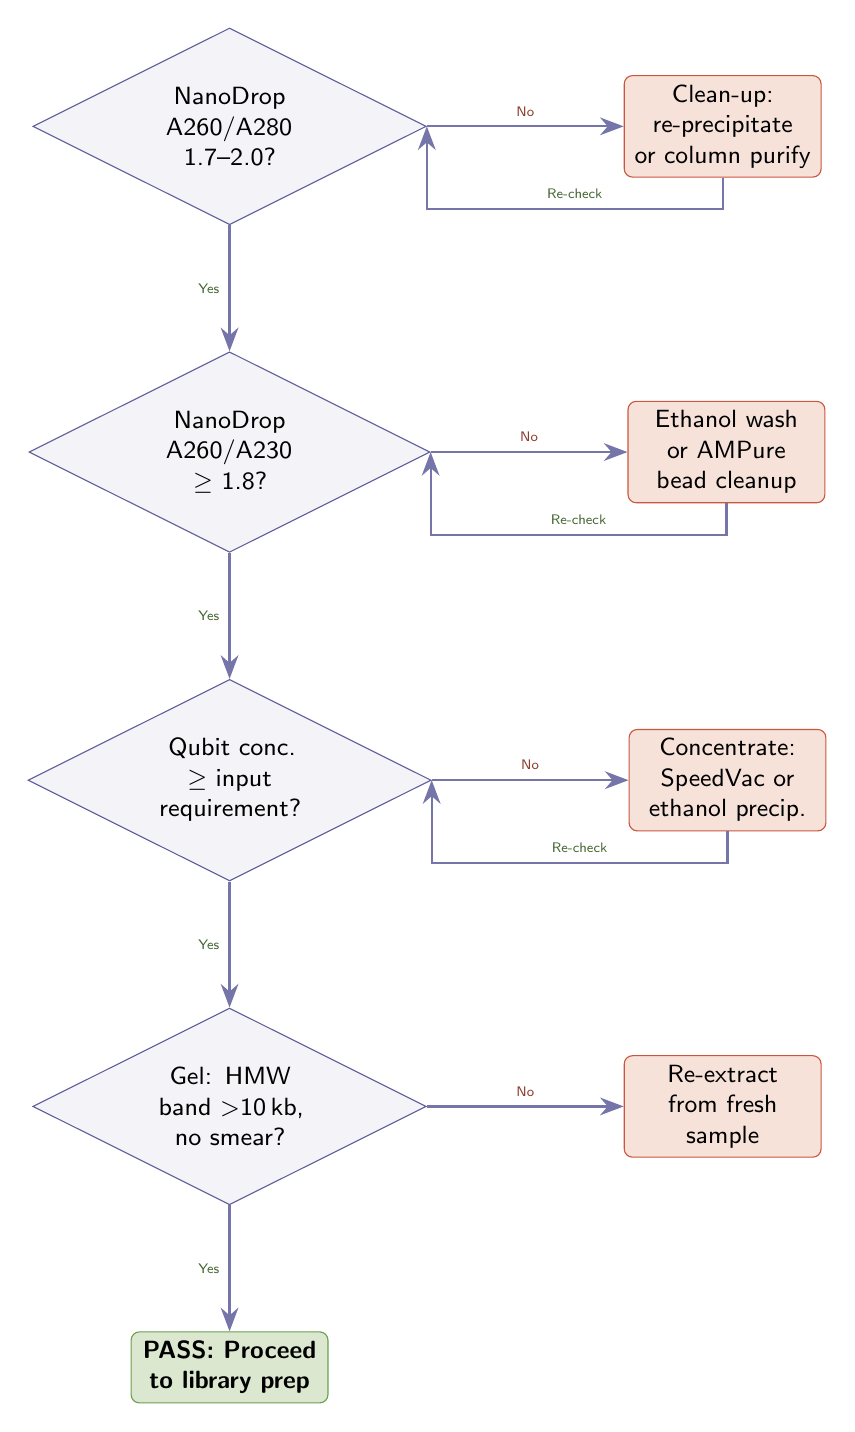
\begin{tikzpicture}[
  >={Stealth[length=3mm]},
  node distance=1.4cm and 2.0cm,
  decision/.style={diamond, draw=MidnightBlue!70, fill=MidnightBlue!5, text width=2.8cm,
    align=center, inner sep=1pt, font=\small\sffamily, aspect=2},
  process/.style={rectangle, draw=OliveGreen!70, fill=OliveGreen!5, rounded corners=3pt,
    minimum width=3cm, minimum height=0.7cm, align=center, font=\small\sffamily},
  fail/.style={rectangle, draw=BrickRed!70, fill=BrickRed!10, rounded corners=3pt,
    minimum width=2.5cm, minimum height=0.7cm, align=center, font=\small\sffamily},
  pass/.style={rectangle, draw=OliveGreen!70, fill=OliveGreen!15, rounded corners=3pt,
    minimum width=2.5cm, minimum height=0.7cm, align=center, font=\small\sffamily\bfseries},
  arr/.style={->, thick, MidnightBlue!60},
  yeslbl/.style={font=\tiny\sffamily, OliveGreen!70!black},
  nolbl/.style={font=\tiny\sffamily, BrickRed!70!black},
]

% NanoDrop 260/280
\node[decision] (nd280) {NanoDrop\\A260/A280\\1.7--2.0?};
\node[fail, right=2.5cm of nd280] (clean1) {Clean-up:\\re-precipitate\\or column purify};

% NanoDrop 260/230
\node[decision, below=1.6cm of nd280] (nd230) {NanoDrop\\A260/A230\\$\geq$ 1.8?};
\node[fail, right=2.5cm of nd230] (clean2) {Ethanol wash\\or AMPure\\bead cleanup};

% Qubit
\node[decision, below=1.6cm of nd230] (qubit) {Qubit conc.\\$\geq$ input\\requirement?};
\node[fail, right=2.5cm of qubit] (conc) {Concentrate:\\SpeedVac or\\ethanol precip.};

% Gel
\node[decision, below=1.6cm of qubit] (gel) {Gel: HMW\\band $>$10\,kb,\\no smear?};
\node[fail, right=2.5cm of gel] (reext) {Re-extract\\from fresh\\sample};

% Pass
\node[pass, below=1.6cm of gel] (proceed) {PASS: Proceed\\to library prep};

% Arrows
\draw[arr] (nd280) -- node[yeslbl, left] {Yes} (nd230);
\draw[arr] (nd280) -- node[nolbl, above] {No} (clean1);
\draw[arr] (clean1.south) -- ++(0,-0.4) -| node[yeslbl, near start, above] {Re-check} (nd280.east);

\draw[arr] (nd230) -- node[yeslbl, left] {Yes} (qubit);
\draw[arr] (nd230) -- node[nolbl, above] {No} (clean2);
\draw[arr] (clean2.south) -- ++(0,-0.4) -| node[yeslbl, near start, above] {Re-check} (nd230.east);

\draw[arr] (qubit) -- node[yeslbl, left] {Yes} (gel);
\draw[arr] (qubit) -- node[nolbl, above] {No} (conc);
\draw[arr] (conc.south) -- ++(0,-0.4) -| node[yeslbl, near start, above] {Re-check} (qubit.east);

\draw[arr] (gel) -- node[yeslbl, left] {Yes} (proceed);
\draw[arr] (gel) -- node[nolbl, above] {No} (reext);

\end{tikzpicture}
\caption[DNA QC decision tree]{Quality control decision tree for extracted DNA. Each sample must pass four sequential checkpoints---NanoDrop purity (A260/A280 and A260/A230), Qubit concentration, and gel electrophoresis---before proceeding to library preparation. Failed samples are routed to cleanup or re-extraction steps.}
\label{fig:protocols:qc_tree}
\end{figure}

\begin{tipbox}[title={NanoDrop vs.\ Qubit: When They Disagree}]
NanoDrop measures absorbance of \emph{everything} at 260\,nm, while Qubit uses a dye specific to dsDNA. When NanoDrop reads much higher than Qubit, non-DNA contaminants are present. \textbf{Always trust Qubit for concentration, NanoDrop for purity ratios only.}
\end{tipbox}

%% ============================================================
\section{Nanopore Rapid Barcoding Kit (SQK-RBK114.96)}
\label{sec:protocols:rbk}
%% ============================================================

The Rapid Barcoding Kit SQK-RBK114.96 is designed for high-throughput multiplexing with minimal hands-on time, using a transposase to simultaneously fragment DNA and attach barcoded adapters.

\begin{keyconcept}[title={Rapid Barcoding: Speed vs.\ Read Length}]
The transposase simultaneously cleaves DNA and attaches barcode adapters, achieving $\sim$15 minutes hands-on time but limiting N50 read length to 5--10\kilobase{}. If long reads ($>$20\kilobase{}) are critical (structural variants, phasing, assembly), use the Ligation Kit SQK-LSK114 instead (\cref{sec:protocols:lsk}).
\end{keyconcept}

\begin{table}[htbp]
\centering
\caption{SQK-RBK114.96 kit specifications and input requirements.}
\label{tab:protocols:rbk_specs}
\small
\renewcommand{\arraystretch}{1.3}
\begin{tabularx}{\textwidth}{@{}l X@{}}
\toprule
\textbf{Parameter} & \textbf{Specification} \\
\midrule
Kit name & Rapid Barcoding Kit 96 V14 \\
Kit code & SQK-RBK114.96 \\
Chemistry & V14 (Kit 14) with 5\,kHz sampling \\
Number of barcodes & 96 unique barcodes \\
Input DNA requirement & 50--200\,ng per sample (100\,ng recommended) \\
Input DNA quality & A260/A280 $\geq$ 1.8; HMW preferred but not required \\
Hands-on time & $\sim$15 minutes \\
Compatible flow cells & R10.4.1 (FLO-MIN114, FLO-PRO114M) \\
Output read N50 & 5--10\kilobase{} (input-dependent) \\
Recommended applications & Amplicon sequencing, surveillance, species ID, low-complexity samples \\
\bottomrule
\end{tabularx}
\end{table}

\begin{protocolbox}[title={Protocol: Nanopore Rapid Barcoding (SQK-RBK114.96)}]
\textbf{Estimated time:} 15 minutes hands-on + 30 minutes barcoding incubation. \textbf{Perform at room temperature unless stated otherwise.}

\textbf{Before you start:}
\begin{itemize}[nosep]
  \item Thaw Rapid Adapter F (RAP~F) on ice and mix by flicking. Spin down briefly.
  \item Thaw barcodes (RB01--RB96) at room temperature. Spin down briefly.
  \item Ensure all DNA samples are quantified by Qubit and normalised to 50\,ng in 5\,$\mu$L with nuclease-free water.
\end{itemize}

\textbf{Barcoding:}
\begin{enumerate}[nosep]
  \item In a 96-well PCR plate or individual PCR strip tubes, combine per sample:
    \begin{itemize}[nosep]
      \item 5\,$\mu$L DNA (50\,ng)
      \item 5\,$\mu$L barcoded rapid adapter (e.g., RB01 for sample 1, RB02 for sample 2, etc.)
    \end{itemize}
  \item Mix by pipetting up and down 5 times. Do not vortex.
  \item Incubate at 30\textdegree C for 2 minutes in a thermal cycler.
  \item Incubate at 80\textdegree C for 2 minutes to heat-inactivate the transposase.
  \item Briefly spin down the plate/tubes. Place on ice.
\end{enumerate}

\textbf{Pooling and adapter attachment:}
\begin{enumerate}[nosep, start=6]
  \item Pool all barcoded samples into a single 1.5\,mL DNA LoBind tube (total volume = $n$ samples $\times$ 10\,$\mu$L).
  \item If pooling $>$24 samples, use only 5\,$\mu$L from each reaction to keep total volume manageable.
  \item Add 1$\times$ volume of AMPure XP beads (e.g., 240\,$\mu$L beads if total pool is 240\,$\mu$L). Mix by gentle flicking.
  \item Incubate at room temperature for 5 minutes.
  \item Place on a magnetic rack for 2 minutes until solution is clear.
  \item Remove and discard the supernatant.
  \item With the tube still on the magnet, wash twice with 200\,$\mu$L freshly prepared 80\% ethanol. Wait 30\,s per wash before removing ethanol.
  \item Remove all residual ethanol with a fine pipette tip. Air-dry for 30 seconds (\textbf{do not over-dry}---nanopore adapters are sensitive to bead over-drying).
  \item Remove tube from magnet. Resuspend beads in 15\,$\mu$L Elution Buffer (EB).
  \item Incubate at room temperature for 2 minutes. Return to magnet for 2 minutes.
  \item Transfer 15\,$\mu$L eluate to a new 1.5\,mL DNA LoBind tube.
  \item Add 1\,$\mu$L Rapid Adapter F (RAP~F). Mix by gentle flicking 10 times.
  \item Incubate at room temperature for 5 minutes.
\end{enumerate}

\textbf{The library is now ready for loading.} Proceed to flow cell priming and loading (\cref{sec:protocols:flowcell}).
\end{protocolbox}

\begin{tipbox}[title={When to Use Rapid Barcoding vs.\ Ligation}]
\textbf{Choose Rapid Barcoding} when speed is paramount, you need $>$24-plex multiplexing, for amplicon sequencing, when input DNA is limited ($<$200\,ng), or for surveillance applications.
\textbf{Choose Ligation} when long reads ($>$10\kilobase{}) are essential (assembly, SVs, phasing), for maximum data yield (1.5--2$\times$ more), or when native DNA modifications must be preserved.
\end{tipbox}

%% ============================================================
\section{Nanopore Ligation Sequencing Kit (SQK-LSK114)}
\label{sec:protocols:lsk}
%% ============================================================

The Ligation Sequencing Kit SQK-LSK114 is the workhorse kit for nanopore sequencing when read length and data yield must be maximised. It uses a multi-step enzymatic preparation (end repair, dA-tailing, adapter ligation) that preserves the full length of input DNA.

\begin{keyconcept}[title={Ligation Libraries Preserve Read Length}]
Without transposase fragmentation, read length directly reflects the input DNA fragment length. With HMW DNA ($>$50\kilobase{}) and gentle handling (wide-bore tips, no vortexing), reads exceeding 100\kilobase{} are achievable. The trade-off: 60--90 minutes hands-on and 1,000\,ng input recommended.
\end{keyconcept}

\begin{protocolbox}[title={Protocol: Nanopore Ligation Sequencing (SQK-LSK114)}]
\textbf{Estimated time:} 60--90 minutes hands-on. \textbf{Input:} 1,000\,ng gDNA in 47\,$\mu$L nuclease-free water.

\textbf{Before you start:}
\begin{itemize}[nosep]
  \item Thaw NEBNext Companion Module reagents: FFPE Repair Buffer, FFPE Repair Mix, Ultra II End Prep Reaction Buffer, Ultra II End Prep Enzyme Mix. Keep on ice.
  \item Thaw Ligation Adapter (LA), Ligation Buffer (LNB), and Quick T4 DNA Ligase. Keep LNB and LA on ice; T4 ligase at $-20$\textdegree C until needed.
  \item Thaw Elution Buffer (EB) and Short Fragment Buffer (SFB). Keep at room temperature.
  \item Prepare fresh 80\% ethanol ($\geq$500\,$\mu$L).
  \item Resuspend AMPure XP beads by vortexing. Equilibrate to room temperature.
  \item Use wide-bore pipette tips throughout to minimise DNA shearing.
\end{itemize}

\textbf{Step 1: DNA repair and end-prep} (combines FFPE repair and end-prep in a single reaction):
\begin{enumerate}[nosep]
  \item In a 0.2\,mL thin-wall PCR tube, combine:
    \begin{itemize}[nosep]
      \item 47\,$\mu$L DNA (1,000\,ng)
      \item 1\,$\mu$L FFPE DNA Repair Buffer
      \item 1\,$\mu$L FFPE DNA Repair Mix
      \item 3.5\,$\mu$L Ultra II End Prep Reaction Buffer
      \item 1.5\,$\mu$L Ultra II End Prep Enzyme Mix
      \item 1\,$\mu$L nuclease-free water
    \end{itemize}
    Total volume: 55\,$\mu$L.
  \item Mix gently by flicking the tube 10--15 times. Do not vortex.
  \item Spin down briefly in a mini centrifuge.
  \item Incubate in a thermal cycler: 20\textdegree C for 5 minutes, then 65\textdegree C for 5 minutes. Hold at 4\textdegree C.
\end{enumerate}

\textbf{Step 2: AMPure XP cleanup} (removes enzymes, buffers, and short fragments):
\begin{enumerate}[nosep, start=5]
  \item Add 55\,$\mu$L (1$\times$ volume) AMPure XP beads to the end-prepped DNA. Mix by gentle flicking.
  \item Incubate at room temperature for 5 minutes.
  \item Place on magnetic rack. Wait 2 minutes until solution clears.
  \item Remove and discard supernatant.
  \item Wash twice with 200\,$\mu$L freshly prepared 80\% ethanol. Wait 30\,s each wash.
  \item Remove residual ethanol with a fine tip. Air-dry for 30 seconds. \textbf{Do not over-dry.}
  \item Remove from magnet. Resuspend in 61\,$\mu$L nuclease-free water. Incubate 2 minutes.
  \item Return to magnet for 2 minutes. Transfer 61\,$\mu$L eluate to a clean tube.
\end{enumerate}

\textbf{Step 3: Adapter ligation:}
\begin{enumerate}[nosep, start=13]
  \item In the eluate tube (61\,$\mu$L end-prepped DNA), add:
    \begin{itemize}[nosep]
      \item 25\,$\mu$L Ligation Buffer (LNB)
      \item 10\,$\mu$L Quick T4 DNA Ligase
      \item 5\,$\mu$L Ligation Adapter (LA)
    \end{itemize}
    Total volume: 101\,$\mu$L.
  \item Mix by gentle flicking 10 times. Spin down briefly.
  \item Incubate at room temperature for 10 minutes.
\end{enumerate}

\textbf{Step 4: AMPure XP cleanup with Short Fragment Buffer:}
\begin{enumerate}[nosep, start=16]
  \item Add 40\,$\mu$L AMPure XP beads (0.4$\times$ ratio for long-fragment selection). Mix gently.
  \item Incubate at room temperature for 5 minutes.
  \item Place on magnetic rack for 2 minutes.
  \item Remove and discard supernatant.
  \item Wash twice with 250\,$\mu$L Short Fragment Buffer (SFB). \textbf{Not ethanol}---SFB is specifically formulated for this step.
  \item Remove residual SFB. Air-dry for 30 seconds.
  \item Remove from magnet. Resuspend in 15\,$\mu$L Elution Buffer (EB). Incubate 2 minutes.
  \item Return to magnet for 2 minutes. Transfer 15\,$\mu$L to a clean 1.5\,mL DNA LoBind tube.
  \item Quantify 1\,$\mu$L by Qubit. Expected: 20--50\,fmol (approximately 50--700\,ng depending on fragment length distribution).
\end{enumerate}

\textbf{The library is now ready for loading.} Proceed to flow cell priming and loading (\cref{sec:protocols:flowcell}).
\end{protocolbox}
\begin{warningbox}[title={Do Not Use Ethanol Washes After Ligation}]
After ligation, wash with Short Fragment Buffer (SFB), \textbf{not} ethanol. Ethanol denatures the motor protein on the adapter, destroying the library---this is the most common ligation prep mistake and produces zero data. SFB removes short fragments while preserving motor protein integrity.
\end{warningbox}

\subsection{AMPure XP Bead Ratio Optimisation}
\label{subsec:protocols:ampure}

The ratio of AMPure XP beads to sample volume determines the size cutoff for DNA fragment retention. Lower ratios select for longer fragments. This is critical for tuning read length distributions.

\begin{table}[htbp]
\centering
\caption{AMPure XP bead ratio and approximate fragment size cutoff for DNA selection.}
\label{tab:protocols:ampure_ratios}
\small
\renewcommand{\arraystretch}{1.3}
\begin{tabularx}{\textwidth}{@{}c c c X@{}}
\toprule
\textbf{Bead:Sample Ratio} & \textbf{Size Cutoff} & \textbf{Recovery \%} & \textbf{Use Case} \\
\midrule
2.0$\times$ & $>$100\basepair{} & $>$95\% & Amplicon cleanup; retain all fragments \\
\addlinespace
1.0$\times$ & $>$200\basepair{} & $>$90\% & Standard cleanup; general-purpose \\
\addlinespace
0.8$\times$ & $>$400\basepair{} & 80--90\% & Post end-prep cleanup; remove adapter dimers \\
\addlinespace
0.6$\times$ & $>$800\basepair{} & 70--85\% & Select for longer fragments; reduce short-fragment noise \\
\addlinespace
0.45$\times$ & $>$1.5\kilobase{} & 60--75\% & Long-read enrichment; post-ligation \\
\addlinespace
0.4$\times$ & $>$2\kilobase{} & 50--70\% & Aggressive long-read selection; recommended for LSK114 \\
\addlinespace
0.35$\times$ & $>$3\kilobase{} & 40--60\% & Ultra-long read enrichment; significant yield loss \\
\bottomrule
\end{tabularx}
\end{table}

\begin{tipbox}[title={Bead Ratio Fine-Tuning}]
Exact cutoffs depend on DNA concentration, buffer composition, and temperature. For critical applications, test 3--4 ratios empirically on a gel or TapeStation. A 0.4$\times$ ratio is the default for SQK-LSK114 post-ligation cleanup; going below 0.35$\times$ causes unacceptable yield loss.
\end{tipbox}

%% ============================================================
\section{16S/ITS Amplicon Library Preparation}
\label{sec:protocols:amplicon}
%% ============================================================

Amplicon sequencing of phylogenetic marker genes is one of the most accessible \acrshort{NGS} applications. Nanopore sequencing enables full-length 16S ($\sim$1,500\basepair{}) and ITS sequencing, providing superior taxonomic resolution compared to short-read approaches targeting single variable regions.

\subsection{Primer Selection}
\label{subsec:protocols:primers}

\begin{table}[htbp]
\centering
\caption{Recommended primers for full-length amplicon nanopore sequencing.}
\label{tab:protocols:primers}
\small
\renewcommand{\arraystretch}{1.3}
\begin{tabularx}{\textwidth}{@{}l l l c X@{}}
\toprule
\textbf{Target} & \textbf{Primer} & \textbf{Sequence (5$'$$\to$3$'$)} & \textbf{Amplicon} & \textbf{Notes} \\
\midrule
16S (bacteria, & 27F & AGAGTTTGATCMTGGCTCAG & \multirow{2}{*}{$\sim$1,465\basepair{}} & Universal bacterial; \\
\quad archaea) & 1492R & TACGGYTACCTTGTTACGACTT & & covers V1--V9 \\
\addlinespace
ITS (fungi) & ITS1f & CTTGGTCATTTAGAGGAAGTAA & \multirow{2}{*}{500--850\basepair{}} & Fungal-biased forward \\
 & ITS4 & TCCTCCGCTTATTGATATGC & & primer; broad coverage \\
\addlinespace
18S (eukaryotes) & Euk-A & AACCTGGTTGATCCTGCCAGT & \multirow{2}{*}{$\sim$1,800\basepair{}} & Broad eukaryotic \\
 & Euk-B & TGATCCTTCTGCAGGTTCACCTAC & & coverage \\
\bottomrule
\end{tabularx}
\end{table}

\begin{tipbox}[title={Adding Barcode Tails to Primers}]
With SQK-RBK114.96, no primer modification is needed---the transposase attaches barcodes directly. For native barcoding (SQK-NBD114.96), add barcode sequences as 5$'$ tails on primers. Consult the \acrshort{ONT} protocol for current tail sequences (these change between kit versions).
\end{tipbox}

\subsection{PCR Cycling Conditions}
\label{subsec:protocols:pcr_cycling}

\begin{table}[htbp]
\centering
\caption{PCR cycling conditions for full-length 16S and ITS amplicon generation.}
\label{tab:protocols:pcr_conditions}
\small
\renewcommand{\arraystretch}{1.3}
\begin{tabularx}{\textwidth}{@{}l c c c X@{}}
\toprule
\textbf{Step} & \textbf{Temperature} & \textbf{Time} & \textbf{Cycles} & \textbf{Notes} \\
\midrule
Initial denaturation & 95\textdegree C & 3 min & 1 & Complete template denaturation \\
Denaturation & 95\textdegree C & 30 s & \multirow{3}{*}{25--30} & Reduce cycles to 25 for high-input samples \\
Annealing & 55\textdegree C & 30 s & & 55\textdegree C works for both 27F/1492R and ITS1f/ITS4 \\
Extension & 72\textdegree C & 90 s & & 1 min/kb; 90\,s for $\sim$1.5\kilobase{} 16S \\
Final extension & 72\textdegree C & 5 min & 1 & Complete all partial products \\
Hold & 4\textdegree C & $\infty$ & --- & Short-term storage \\
\bottomrule
\end{tabularx}
\end{table}

\begin{protocolbox}[title={Protocol: 16S Amplicon PCR (25\,$\mu$L Reaction)}]
\textbf{Per reaction:}
\begin{itemize}[nosep]
  \item 12.5\,$\mu$L LongAmp Taq 2$\times$ Master Mix (NEB, Cat.\ No.\ M0287)
  \item 1\,$\mu$L forward primer 27F (10\,$\mu$M stock)
  \item 1\,$\mu$L reverse primer 1492R (10\,$\mu$M stock)
  \item 1\,$\mu$L template DNA (1--10\,ng)
  \item 9.5\,$\mu$L nuclease-free water
\end{itemize}

\textbf{Cycling:} Use the conditions in \cref{tab:protocols:pcr_conditions} with 25--30 cycles.

\textbf{Post-PCR:}
\begin{enumerate}[nosep]
  \item Confirm amplification by running 2\,$\mu$L on a 1\% agarose gel (expect a single band at $\sim$1,465\basepair{}).
  \item Clean up with 0.8$\times$ AMPure XP beads to remove primers and dimers.
  \item Quantify by Qubit dsDNA BR assay.
  \item Normalise all samples to the same concentration before pooling for barcoding.
\end{enumerate}
\end{protocolbox}

\subsection{Barcoding Strategy and Controls}
\label{subsec:protocols:barcoding}

For multiplexed amplicon experiments, proper barcoding and controls are essential:

\begin{itemize}[nosep]
  \item \textbf{Barcode assignment:} Assign unique barcodes to each sample with a mapping sheet linking barcodes to sample identifiers and metadata.
  \item \textbf{Positive control:} Include a mock community (e.g., ZymoBIOMICS Microbial Community Standard, D6300: 8 bacteria + 2 fungi at known ratios) to assess classification accuracy.
  \item \textbf{Negative controls:} Include \textbf{both} an extraction blank and a \acrshort{PCR} no-template control (NTC). Both must be barcoded and sequenced. Taxa in negatives indicate contamination.
  \item \textbf{Balanced pooling:} Aim for equimolar pooling to ensure even read distribution across samples.
\end{itemize}
\begin{warningbox}[title={The ``Kitome'' Problem}]
Extraction kits and \acrshort{PCR} reagents contain trace bacterial DNA (``kitome''). In low-biomass samples these contaminants can dominate results. Common kitome genera: \species{Bradyrhizobium}, \species{Ralstonia}, \species{Methylobacterium}, \species{Sphingomonas}. Extraction blanks are the only way to identify and remove these contaminants. Never omit them.
\end{warningbox}

%% ============================================================
\section{Loading and Running the Flow Cell}
\label{sec:protocols:flowcell}
%% ============================================================

The final steps are flow cell quality assessment, priming, library loading, and run monitoring.

\subsection{Flow Cell QC Check}
\label{subsec:protocols:flowcell_qc}

Before loading any library, verify that the flow cell has sufficient active nanopores.

\begin{protocolbox}[title={Protocol: Flow Cell Quality Check}]
\begin{enumerate}[nosep]
  \item Insert the R10.4.1 flow cell (FLO-MIN114) into the MinION or GridION device.
  \item Open \software{MinKNOW} software. Navigate to the flow cell check (or ``Platform QC'') function.
  \item Initiate the flow cell check. The software will apply a voltage and measure current through each pore (takes $\sim$5 minutes).
  \item Read the result:
    \begin{itemize}[nosep]
      \item \textbf{$>$800 active pores:} Excellent. Proceed with loading.
      \item \textbf{600--800 active pores:} Acceptable. Expect slightly reduced throughput.
      \item \textbf{$<$600 active pores:} Contact \acrshort{ONT} support for a replacement. Running a library on a low-pore flow cell is not cost-effective.
    \end{itemize}
  \item Record the pore count in your laboratory notebook for later reference.
\end{enumerate}
\end{protocolbox}

\subsection{Flow Cell Priming}
\label{subsec:protocols:priming}

Priming replaces storage buffer with sequencing-compatible buffer and removes air bubbles from the sensor array.

\begin{protocolbox}[title={Protocol: Flow Cell Priming (R10.4.1)}]
\textbf{Prepare the priming mix:}
\begin{enumerate}[nosep]
  \item Thaw one tube of Flow Cell Flush (FCF) at room temperature. Briefly spin down.
  \item Add 30\,$\mu$L of Flow Cell Tether (FCT) to the FCF tube. Mix by gentle inversion. This is the Priming Mix.
\end{enumerate}

\textbf{Prime the flow cell:}
\begin{enumerate}[nosep, start=3]
  \item Open the priming port on the flow cell by sliding the cover clockwise. \textbf{Do not remove the SpotON port cover yet.}
  \item Set a P1000 pipette to 200\,$\mu$L. Insert the tip into the priming port. Turn the pipette dial to draw back a small amount of buffer ($\sim$20--30\,$\mu$L) until you see a small amount of buffer entering the tip. This removes any air bubble from the sensor array.
  \item Load 800\,$\mu$L of Priming Mix via the priming port. Allow to flow through by gravity (do not force). Wait 5 minutes.
  \item Open the SpotON port cover.
  \item Load another 200\,$\mu$L of Priming Mix via the priming port.
\end{enumerate}
\end{protocolbox}

\subsection{Library Loading}
\label{subsec:protocols:loading}

\begin{protocolbox}[title={Protocol: Library Loading}]
\textbf{Prepare the loading mix:}
\begin{enumerate}[nosep]
  \item In a clean 1.5\,mL tube, combine:
    \begin{itemize}[nosep]
      \item 37\,$\mu$L Sequencing Buffer (SB)
      \item 25.5\,$\mu$L Loading Beads (LB)---\textbf{mix thoroughly by pipetting immediately before use}, as beads settle rapidly
      \item 12\,$\mu$L prepared library (from SQK-LSK114 or SQK-RBK114.96)
    \end{itemize}
    Total volume: 75\,$\mu$L.
  \item Mix by gentle pipetting. Do not vortex.
\end{enumerate}

\textbf{Load the library:}
\begin{enumerate}[nosep, start=3]
  \item Using a P200 pipette, add the entire 75\,$\mu$L \textbf{drop-by-drop} through the SpotON port. Ensure each drop is drawn into the flow cell before adding the next (you will see each drop wick into the port).
  \item Close the SpotON port cover.
  \item Close the priming port cover.
  \item Close the MinION/GridION lid.
\end{enumerate}
\end{protocolbox}
\begin{warningbox}[title={Loading Beads Must Be Mixed}]
Loading Beads settle within seconds. Pipette-mix thoroughly immediately before adding to the loading mix and load promptly. Settled beads cause very low pore occupancy and minimal output.
\end{warningbox}

\subsection{MinKNOW Run Setup and Monitoring}
\label{subsec:protocols:minknow}

\begin{protocolbox}[title={Protocol: Starting a Sequencing Run in MinKNOW}]
\begin{enumerate}[nosep]
  \item In \software{MinKNOW}, select ``Start Sequencing.''
  \item Configure run parameters:
    \begin{itemize}[nosep]
      \item \textbf{Kit:} Select the kit used (SQK-RBK114.96 or SQK-LSK114).
      \item \textbf{Basecalling:} Select ``Super accuracy'' (SUP) model for highest accuracy ($>$Q20 modal). Alternatively, use ``Fast'' basecalling if real-time analysis is needed and accuracy requirements are lower.
      \item \textbf{Barcoding:} If using rapid barcoding, enable barcode detection and select the appropriate barcode kit.
      \item \textbf{Run length:} Default 72 hours. For rapid experiments or flow cell reuse, set to 24 hours.
      \item \textbf{Output format:} FASTQ (for immediate analysis) or POD5 (raw signal, for re-basecalling).
    \end{itemize}
  \item Click ``Start'' to begin sequencing.
\end{enumerate}

\textbf{Monitoring parameters to check during the run:}
\begin{itemize}[nosep]
  \item \textbf{Pore occupancy:} Target $>$50\%. If below 20\%, the library loading was unsuccessful---check loading bead mixing.
  \item \textbf{Strand rate:} Number of reads translating per minute. Should be steady or slowly declining.
  \item \textbf{Read length distribution:} Should match expectations for your library type (5--10\kilobase{} N50 for rapid, $>$10\kilobase{} for ligation).
  \item \textbf{Quality score distribution:} Modal quality should be $>$Q15 (fast basecalling) or $>$Q20 (SUP basecalling).
  \item \textbf{Active pore count:} Will decline over 72 hours. A rapid drop in the first hour may indicate a problem (contaminated library, air bubbles, or membrane damage).
  \item \textbf{Temperature:} The device should maintain 35\textdegree C. Overheating causes increased noise.
\end{itemize}
\end{protocolbox}

\subsection{Nuclease Flush and Reload}
\label{subsec:protocols:flush}

If a run completes before 72 hours and active pores remain, flush and reload a new library to maximise flow cell utilisation.

\begin{protocolbox}[title={Protocol: Nuclease Flush and Reload}]
\begin{enumerate}[nosep]
  \item In \software{MinKNOW}, stop the current sequencing run.
  \item Prepare wash solution: add 380\,$\mu$L nuclease-free water to one tube of DNase I from the Flow Cell Wash Kit (EXP-WSH004). Mix by inversion.
  \item Open the priming port and SpotON port covers on the flow cell.
  \item Using a P1000 pipette, slowly draw off all the library from the priming port. Discard.
  \item Load 400\,$\mu$L of the DNase I wash solution via the priming port.
  \item Close both port covers. Leave at room temperature for 30 minutes. The DNase will digest remaining DNA and free the pores.
  \item After 30 minutes, open both port covers and remove the wash solution via the priming port.
  \item Re-prime the flow cell with fresh Priming Mix (as in the priming protocol, \cref{subsec:protocols:priming}).
  \item Perform a flow cell check to assess remaining active pore count.
  \item If $>$400 pores remain, load a new library via the SpotON port.
  \item Start a new sequencing run in \software{MinKNOW}.
\end{enumerate}
\end{protocolbox}
\begin{tipbox}[title={Maximising Flow Cell Value}]
A single R10.4.1 flow cell can be reused 2--3 times with nuclease flushes. Use the first load for the most important library (best pore count). Each reload typically yields 50--70\% of the previous run's output. Store partially used flow cells at 4\textdegree C for up to one week.
\end{tipbox}

%% ============================================================
\section{Troubleshooting}
\label{sec:protocols:troubleshooting}
%% ============================================================

\centering
\small
\renewcommand{\arraystretch}{1.3}
\begin{longtable}{@{}p{3.5cm} p{4.5cm} p{6.5cm}@{}}
\caption{Comprehensive troubleshooting guide for nanopore sequencing workflows.}
\label{tab:protocols:troubleshooting}\\
\toprule
\textbf{Problem} & \textbf{Likely Cause} & \textbf{Solution} \\
\midrule
\endfirsthead
\toprule
\textbf{Problem} & \textbf{Likely Cause} & \textbf{Solution} \\
\midrule
\endhead
\midrule
\multicolumn{3}{r}{\textit{Continued on next page}} \\
\bottomrule
\endfoot
\bottomrule
\endlastfoot

Very low yield after extraction & Insufficient lysis or input material & Increase incubation time with Proteinase K; increase sample input volume; check expiry of lysis reagents \\
\addlinespace

A260/A280 $<$ 1.7 & Protein or phenol contamination & Re-precipitate DNA; run through a cleanup column; extend Proteinase K digestion \\
\addlinespace

A260/A230 $<$ 1.5 & Guanidinium, ethanol, or chaotropic salt carry-over & Additional ethanol wash steps; column cleanup; ensure full 3-min drying spin \\
\addlinespace

Degraded DNA (smear on gel) & Nuclease activity, improper storage, or excessive handling & Use fresh reagents; store DNA at $-20$\textdegree C; minimise freeze-thaw cycles; add EDTA to storage buffer \\
\addlinespace

Low pore occupancy ($<$20\%) & Insufficient library, loading bead settling, or air bubbles & Re-quantify library; ensure beads are mixed immediately before loading; remove air from priming port \\
\addlinespace

Pore occupancy drops rapidly in first hour & Library quality issue or membrane contamination & Check for contaminants (detergent, organic solvents); re-prepare library from clean DNA \\
\addlinespace

Short reads ($<$1\kilobase{} N50) with ligation kit & DNA shearing during preparation & Use wide-bore pipette tips; do not vortex; handle tubes gently; avoid freeze-thaw of HMW DNA \\
\addlinespace

No reads after starting run & Adapter not attached or motor protein denatured & Verify adapter ligation with Qubit (concentration should not drop $>$50\%); check that SFB (not ethanol) was used for post-ligation wash \\
\addlinespace

High adapter dimer reads & Excessive adapter in ligation reaction or insufficient cleanup & Lower adapter input; use a stricter AMPure bead ratio (0.4$\times$); check for DNA input below minimum \\
\addlinespace

Low quality scores ($<$Q10 modal) & Old flow cell, basecalling model mismatch, or temperature issue & Use SUP basecalling model; check flow cell manufacture date; ensure device is not overheating \\
\addlinespace

Uneven barcode distribution & Unequal DNA input or PCR amplification bias & Quantify all samples by Qubit and normalise to equimolar before pooling; reduce PCR cycle number \\
\addlinespace

High ``unclassified'' barcode reads & Poor barcode ligation or chimeric reads & Increase barcode stringency in \software{MinKNOW}; check DNA input was not degraded \\
\addlinespace

No amplicon band on gel & Primer failure, inhibitors, or template issue & Check primer sequences and concentrations; run positive control; dilute template 1:10 to reduce inhibitors \\
\addlinespace

Multiple amplicon bands & Non-specific priming or contamination & Increase annealing temperature (+2--5\textdegree C); reduce primer concentration; use fresh aliquot of primers \\
\addlinespace

MinKNOW software crashes & Insufficient disk space or RAM & Ensure $>$100\,GB free disk space; close other applications; restart software \\
\addlinespace

Temperature warning in MinKNOW & Blocked ventilation or ambient temperature too high & Ensure device ventilation is unobstructed; reduce ambient temperature; use external cooling fan \\
\addlinespace

Flow cell check shows 0 pores & Flow cell not inserted properly or damaged & Remove and reinsert flow cell firmly; check connector pins; try a different flow cell \\
\addlinespace

Mux scan shows declining pores & Normal pore attrition over time or membrane fouling & Normal for runs $>$24\,h; consider nuclease flush and reload to recover pores \\

\end{longtable}

\begin{tipbox}[title={Keep a Sequencing Log}]
Record every run: date, operator, flow cell ID, pore count, kit, DNA input, run time, total reads, N50, and anomalies. This record is invaluable for diagnosing problems and tracking performance.
\end{tipbox}

%% ============================================================
\section{Sample Collection Best Practices}
\label{sec:protocols:collection}
%% ============================================================

The best laboratory protocols cannot rescue a poorly collected sample. This section covers collection, preservation, storage, and documentation best practices.

\subsection{Field Preservation Methods}
\label{subsec:protocols:preservation}

Different sample types require different preservation strategies to maintain DNA integrity:

\begin{description}[style=nextline]
  \item[Cold chain (ice/dry ice)] The default method. Wet ice (4\textdegree C) for transport $<$6 hours; dry ice ($-78$\textdegree C) for overnight shipping. Transfer to $-20$\textdegree C or $-80$\textdegree C upon arrival.
  \item[Chemical preservation] For field situations without cold chain: \textbf{95\% ethanol} ($\geq$10$\times$ volume, stable months at RT); \textbf{RNAlater} (RNA preservation, tissue $<$0.5\,cm in 5$\times$ volume; can interfere with DNA kits); \textbf{DESS buffer} (20\% DMSO, 0.25\,M EDTA, NaCl-saturated, pH 8.0; versatile); \textbf{Longmire's buffer} (100\,mM Tris, 100\,mM EDTA, 10\,mM NaCl, 0.5\% SDS, pH 8.0; eDNA filters and wildlife tissue).
  \item[Desiccation] Silica gel packets in sealed bags for plant leaf tissue. DNA stable for years when dry.
  \item[FTA cards] Cellulose cards lyse cells on contact; DNA stable at RT for years. Punch a disc directly into the \acrshort{PCR} reaction.
  \item[Saliva kits] DNA Genotek OG-500/OG-600 tubes preserve DNA at RT for $>$12 months. See \cref{subsec:protocols:saliva}.
\end{description}

\subsection{Storage Temperature Requirements}
\label{subsec:protocols:storage}

\begin{table}[htbp]
\centering
\caption{Recommended storage conditions and maximum holding times for common sample types.}
\label{tab:protocols:storage}
\small
\renewcommand{\arraystretch}{1.3}
\begin{tabularx}{\textwidth}{@{}l c c X@{}}
\toprule
\textbf{Sample Type} & \textbf{Temperature} & \textbf{Max.\ Hold Time} & \textbf{Notes} \\
\midrule
Whole blood (EDTA) & 4\textdegree C & 7 days & DNA quality declines after 3 days; freeze for longer storage \\
\addlinespace
Whole blood (EDTA) & $-20$\textdegree C & 5 years & Avoid repeated freeze-thaw \\
\addlinespace
Saliva (stabilised) & Room temp & 12 months & DNA Genotek OG-500 buffer \\
\addlinespace
Fresh tissue & 4\textdegree C & 24 hours & Extract ASAP or snap-freeze \\
\addlinespace
Fresh tissue & $-80$\textdegree C & 10+ years & Flash-freeze in liquid nitrogen before transfer \\
\addlinespace
Tissue in 95\% ethanol & Room temp & 6 months & Use $\geq$10$\times$ volume ethanol \\
\addlinespace
Tissue in RNAlater & $-20$\textdegree C & Indefinite & Best for RNA; acceptable for DNA \\
\addlinespace
Stool (fresh) & 4\textdegree C & 24 hours & Use OMNIgene Gut kit for room temp stability \\
\addlinespace
eDNA filter (dry) & $-20$\textdegree C & 6 months & Add preservation buffer for longer storage \\
\addlinespace
eDNA filter (in buffer) & $-20$\textdegree C & 12 months & Longmire's or ATL buffer \\
\addlinespace
Extracted DNA & $-20$\textdegree C & 2+ years & TE buffer or nuclease-free water; avoid freeze-thaw \\
\addlinespace
Extracted DNA & $-80$\textdegree C & 10+ years & Long-term archival storage \\
\addlinespace
Prepared library & 4\textdegree C & 1 week & Load promptly for best results \\
\addlinespace
FFPE blocks & Room temp & 10+ years & DNA is degraded; expect 200--500\basepair{} fragments \\
\addlinespace
Plant leaf (silica-dried) & Room temp & 5+ years & Use indicating silica gel; keep dry \\
\bottomrule
\end{tabularx}
\end{table}

\subsection{Chain of Custody Documentation}
\label{subsec:protocols:custody}

For clinical, forensic, or regulatory applications, a formal chain of custody must be maintained. Even for research, robust sample tracking prevents costly errors. Assign a \textbf{unique sample ID} at collection using a systematic scheme (e.g., ``EDNA-LK01-20260315-W01''). Label tubes with both human-readable text and machine-readable identifiers (barcode/QR code labels; use cryogenic labels for $-80$\textdegree C storage). Maintain a \textbf{chain of custody log} recording collector, date, location (GPS coordinates), preservation method, and every transfer between personnel. Photograph collection sites and sample tubes. Keep both physical (lab notebook) and digital (spreadsheet, LIMS) records.

\subsection{Metadata Recording}
\label{subsec:protocols:metadata}

The biological value of sequencing data depends critically on its associated metadata. Record the following at minimum:

\begin{table}[htbp]
\centering
\caption{Essential metadata fields for sequencing sample documentation.}
\label{tab:protocols:metadata}
\small
\renewcommand{\arraystretch}{1.3}
\begin{tabularx}{\textwidth}{@{}l l X@{}}
\toprule
\textbf{Field} & \textbf{Format} & \textbf{Description} \\
\midrule
Sample ID & Text & Unique identifier linking to all downstream data \\
Collection date & YYYY-MM-DD & ISO 8601 format \\
Collection time & HH:MM (24h) & Local time with timezone noted \\
Collector & Text & Name of person who collected the sample \\
Location & Decimal degrees & Latitude, longitude (GPS); include altitude if relevant \\
Habitat/site & Text & Description of collection environment \\
Sample type & Controlled vocab & e.g., ``saliva'', ``water-eDNA'', ``leaf-tissue'', ``soil'' \\
Organism & Binomial & \species{Homo sapiens}, ``environmental'', or target species \\
Preservation & Controlled vocab & e.g., ``ethanol-95pct'', ``frozen-80C'', ``OG500-stabiliser'' \\
Storage temp & \textdegree C & Temperature at which sample is stored \\
Extraction date & YYYY-MM-DD & Date DNA was extracted \\
Extraction method & Text & Kit name, catalogue number, and any modifications \\
DNA conc. (Qubit) & ng/$\mu$L & Qubit fluorometric measurement \\
A260/A280 & Ratio & NanoDrop purity ratio \\
A260/A230 & Ratio & NanoDrop purity ratio \\
Notes & Free text & Any anomalies, deviations from protocol, or observations \\
\bottomrule
\end{tabularx}
\end{table}

\begin{tipbox}[title={Use Standardised Metadata Standards}]
Align metadata with GSC MIxS (Minimum Information about any (x) Sequence) checklists and \acrshort{SRA} submission requirements from the outset---recording these at collection saves hours of retroactive data entry. See \cref{ch:datastandards} for details on data standards.
\end{tipbox}

\begin{warningbox}[title={Metadata Cannot Be Reconstructed}]
Metadata lost at collection is gone forever. Make metadata recording a non-negotiable part of every field protocol. Pre-print field data sheets or use mobile apps (KoboToolbox, ODK Collect) to ensure completeness.
\end{warningbox}

%% ============================================================
\section{Chapter Summary}
\label{sec:protocols:summary}
%% ============================================================

\begin{keyconcept}[title={Key Takeaways}]
\begin{enumerate}[nosep]
  \item \textbf{Safety is non-negotiable.} Understand your BSL requirements, PPE needs, and chemical hazards before starting any protocol.
  \item \textbf{DNA quality determines sequencing success.} Use the \acrshort{QC} decision tree (\cref{fig:protocols:qc_tree}) to verify every sample before committing it to an expensive flow cell.
  \item \textbf{Choose the right kit for the job.} Rapid Barcoding (SQK-RBK114.96) for speed and high multiplexing; Ligation (SQK-LSK114) for long reads and maximum yield.
  \item \textbf{Never use ethanol washes after ligation.} Use Short Fragment Buffer (SFB) to preserve motor protein integrity.
  \item \textbf{Mix loading beads immediately before use.} Settled beads result in zero pore occupancy.
  \item \textbf{Controls are essential.} Every amplicon experiment requires positive controls (mock community) and negative controls (extraction blank + \acrshort{PCR} NTC).
  \item \textbf{Metadata matters as much as sequence data.} Record comprehensive metadata at the point of collection---it cannot be reconstructed later.
  \item \textbf{Keep a sequencing log.} Track every run's parameters and performance for long-term quality management.
\end{enumerate}
\end{keyconcept}

\chapter{DIY Analysis: From Raw Reads to Results}
\label{ch:diyanalysis}

\begin{keyconcept}
This chapter is your hands-on laboratory notebook for long-read nanopore data analysis. We walk through every step---from configuring your computer and basecalling raw signal data to assembling bacterial genomes, identifying species from metagenomic samples, and calling variants in human genomes. Every command is given in full, every parameter is explained, and complete workflow implementations in both \textbf{Snakemake} and \textbf{Nextflow} are provided so that you can reproduce each analysis end-to-end. Whether you are a bench scientist running your first MinION experiment or a bioinformatician building production pipelines, this chapter gives you the tools to go from raw reads to publication-ready results on your own hardware.
\end{keyconcept}

Throughout this chapter we assume you are working with Oxford Nanopore Technologies (\acrshort{ONT}) data, although many of the downstream tools (assembly, annotation, variant calling) apply equally to PacBio long reads. Where commands differ between platforms, we note the alternatives. All tools are open-source and freely available through \software{conda}/\software{mamba}.

%% ============================================================
\section{Setting Up Your Environment}
\label{sec:diyanalysis:setup}
%% ============================================================

Before you can analyse a single read, you need a properly configured computing environment. This section covers hardware requirements, software installation, and test datasets you can use to validate your setup.

\subsection{Hardware Requirements}
\label{subsec:diyanalysis:hardware}

The computational demands of long-read analysis vary enormously depending on the task. \Cref{tab:diy_hardware} summarises minimum and recommended hardware for the analyses covered in this chapter.

\begin{table}[htbp]
\centering
\caption{Hardware requirements for nanopore data analysis.}
\label{tab:diy_hardware}
\begin{tabularx}{\textwidth}{@{}lXX@{}}
\toprule
\textbf{Component} & \textbf{Minimum} & \textbf{Recommended} \\
\midrule
CPU & 4 cores (Intel i5 / AMD Ryzen 5) & 8+ cores (Intel i7/i9 / AMD Ryzen 7/9) \\
RAM & 8\,GB & 32\,GB (64\,GB for human genomes) \\
Storage & 256\,GB SSD (SATA) & 1\,TB+ NVMe SSD \\
GPU & None (CPU basecalling only) & NVIDIA RTX 3060+ (8\,GB VRAM) for Dorado \\
OS & Ubuntu 20.04+ / macOS 12+ & Ubuntu 22.04 LTS \\
Network & Broadband for tool downloads & High-speed for SRA downloads \\
\bottomrule
\end{tabularx}
\end{table}

\begin{warningbox}[title={Storage Fills Up Fast}]
A single MinION flow cell produces 10--50\,GB of POD5 raw signal data. After basecalling, the resulting \acrshort{BAM} file can be 5--20\,GB. During assembly, temporary files can consume 3--5$\times$ the input size. Monitor disk usage with \texttt{df -h} and plan for at least 3$\times$ the raw data size in free space. NVMe SSDs are strongly recommended---assembly tools like \software{Flye} perform heavy random I/O that is painfully slow on spinning hard drives.
\end{warningbox}

\subsection{Installing Software with Conda}
\label{subsec:diyanalysis:conda}

We use \software{mamba} (a fast drop-in replacement for \software{conda}) and the \texttt{bioconda} channel to install all tools into isolated environments, preventing version conflicts.

\begin{lstlisting}[language=bash,caption={Installing Miniforge and creating the analysis environment.},label=lst:diy-conda-setup]
# Step 1: Install Miniforge (includes mamba)
curl -L -O https://github.com/conda-forge/miniforge/releases/\
latest/download/Miniforge3-Linux-x86_64.sh
bash Miniforge3-Linux-x86_64.sh
# Restart your shell or run: source ~/.bashrc

# Step 2: Create the nanopore analysis environment
mamba create -n nanopore -c conda-forge -c bioconda \
  dorado=0.8.0 \
  nanoplot=1.42.0 \
  pycoqc=2.5.2 \
  fastqc=0.12.1 \
  multiqc=1.21 \
  chopper=0.9.0 \
  flye=2.9.5 \
  medaka=2.0.1 \
  quast=5.2.0 \
  busco=5.7.1 \
  bakta=1.9.4 \
  kraken2=2.1.3 \
  bracken=2.9 \
  krona=2.8.1 \
  minimap2=2.28 \
  samtools=1.21 \
  bcftools=1.21 \
  snakemake=8.25.0 \
  nextflow=24.04.0

# Step 3: Activate the environment
mamba activate nanopore

# Step 4: Verify key tools
dorado --version
flye --version
minimap2 --version
samtools --version | head -1

# Step 5: Export for reproducibility
mamba env export > environment.yml
\end{lstlisting}

\begin{tipbox}[title={Separate Environments for Conflicting Tools}]
Some tools have conflicting dependencies. If \software{mamba create} fails due to unsolvable conflicts, split tools into separate environments. For example, \software{Clair3} often requires its own environment. Use \texttt{mamba create -n clair3 -c bioconda clair3} separately. Snakemake and Nextflow can activate different environments per rule/process automatically.
\end{tipbox}

\subsection{Test Datasets}
\label{subsec:diyanalysis:testdata}

Practise with real-world datasets before analysing your own data. \Cref{tab:diy_testdata} lists publicly available nanopore datasets suitable for the walkthroughs in this chapter.

\begin{table}[htbp]
\centering
\caption{Recommended test datasets from the \acrshort{SRA} and other public repositories.}
\label{tab:diy_testdata}
\begin{tabularx}{\textwidth}{@{}llXl@{}}
\toprule
\textbf{Walkthrough} & \textbf{Accession} & \textbf{Description} & \textbf{Size} \\
\midrule
Bacterial assembly & SRR28370649 & \species{E. coli} K-12 MG1655, R10.4.1, SUP basecall & $\sim$1.5\,GB \\
Bacterial assembly & ERR3813594 & \species{E. coli} K-12, R9.4.1 & $\sim$2.0\,GB \\
Metagenomics & SRR27498888 & ZymoBIOMICS mock community, R10.4.1 & $\sim$3.0\,GB \\
Human variant calling & HG002 (GIAB) & Genome in a Bottle, ONT R10.4.1, chr20 subset & $\sim$5.0\,GB \\
\bottomrule
\end{tabularx}
\end{table}

\begin{lstlisting}[language=bash,caption={Downloading test data from the SRA.},label=lst:diy-download]
# Install SRA Toolkit if not already present
mamba install -c bioconda sra-tools

# Download E. coli test dataset
prefetch SRR28370649
fasterq-dump --threads 4 SRR28370649 -O data/ecoli/

# For BAM input (preferred for ONT data)
# Many ONT datasets are deposited as uBAM; check the SRA entry
wget -P data/ecoli/ \
  https://sra-pub-src-1.s3.amazonaws.com/SRR28370649/reads.bam

# Verify download integrity
samtools quickcheck data/ecoli/reads.bam && echo "OK" || echo "CORRUPT"
\end{lstlisting}

%% ============================================================
\section{Basecalling with Dorado}
\label{sec:diyanalysis:basecalling}
%% ============================================================

Basecalling is the process of converting raw electrical signal data (POD5 files) into nucleotide sequences. \software{Dorado} is Oxford Nanopore's current production basecaller, replacing the older \software{Guppy}. It supports GPU acceleration and produces output directly in \acrshort{BAM} format.

\subsection{Basecalling Models}
\label{subsec:diyanalysis:models}

Dorado offers three model tiers that trade speed for accuracy. \Cref{tab:diy_models} compares them.

\begin{table}[htbp]
\centering
\caption{Dorado basecalling model comparison (R10.4.1 chemistry, v4.3.0 models).}
\label{tab:diy_models}
\begin{tabularx}{\textwidth}{@{}lccXc@{}}
\toprule
\textbf{Model} & \textbf{Simplex Accuracy} & \textbf{Speed (GPU)} & \textbf{Use Case} & \textbf{GPU Required?} \\
\midrule
\texttt{fast} & $\sim$Q15 (96.8\%) & $\sim$5$\times$10$^6$ bases/s & Real-time monitoring, quick previews & Recommended \\
\texttt{hac} & $\sim$Q20 (99.0\%) & $\sim$2$\times$10$^6$ bases/s & Standard analyses, metagenomics & Recommended \\
\texttt{sup} & $\sim$Q23 (99.5\%) & $\sim$0.5$\times$10$^6$ bases/s & Variant calling, assembly, publication-quality & Required \\
\bottomrule
\end{tabularx}
\end{table}

\begin{keyconcept}[title={Which Model Should I Use?}]
For bacterial genome assembly and metagenomics, \texttt{hac} (high-accuracy) is usually sufficient and 4$\times$ faster than \texttt{sup}. For variant calling in human or complex genomes where every tenth of a percent of accuracy matters, always use \texttt{sup} (super-accuracy). Never use \texttt{fast} for any downstream analysis that requires accurate consensus---it is intended only for real-time monitoring during sequencing.
\end{keyconcept}

\subsection{Running Dorado}
\label{subsec:diyanalysis:dorado_run}

\begin{lstlisting}[language=bash,caption={Basecalling with Dorado.},label=lst:diy-dorado]
# List available models
dorado download --list

# Download the SUP model for R10.4.1 chemistry
dorado download --model dna_r10.4.1_e8.2_400bps_sup@v4.3.0

# Basecall POD5 files to unaligned BAM
dorado basecaller \
  dna_r10.4.1_e8.2_400bps_sup@v4.3.0 \
  pod5_dir/ \
  --device cuda:0 \
  --emit-moves \
  > basecalled.bam

# Check the output
samtools view -c basecalled.bam   # total reads
samtools stats basecalled.bam | grep "average length"

# If you need FASTQ output instead (some tools require it)
samtools fastq basecalled.bam | gzip > basecalled.fastq.gz
\end{lstlisting}

\begin{warningbox}[title={GPU vs CPU Basecalling}]
CPU basecalling with the \texttt{sup} model is extremely slow---a single MinION flow cell can take \textbf{days to weeks} on a modern CPU. With an NVIDIA RTX 4090, the same data takes approximately 2--4 hours. If you do not have a GPU, consider: (1) using the \texttt{fast} or \texttt{hac} model, (2) using a cloud GPU instance (see \cref{sec:diyanalysis:cloud}), or (3) using the basecalled data already produced by MinKNOW during the sequencing run. The \texttt{--device cpu} flag forces CPU mode: \texttt{dorado basecaller model pod5/ --device cpu > out.bam}.
\end{warningbox}

\subsection{Understanding BAM Output}
\label{subsec:diyanalysis:bam_output}

Dorado produces \textbf{unaligned BAM} files (uBAM). Unlike traditional aligned BAM files, these contain sequence and quality scores but no alignment information. The key advantage of uBAM over \acrshort{FASTQ} is that it preserves rich metadata:

\begin{itemize}[nosep]
  \item \textbf{Move table}: Signal-to-base correspondence for re-basecalling or modified-base calling.
  \item \textbf{Read group information}: Flow cell ID, run ID, basecall model version.
  \item \textbf{Base modification tags}: If modified-base calling was enabled (\texttt{--modified-bases 5mCG\_5hmCG}).
  \item \textbf{Duplex information}: If duplex basecalling was performed.
\end{itemize}

\begin{lstlisting}[language=bash,caption={Inspecting uBAM metadata.},label=lst:diy-bam-inspect]
# View the header (contains read group and program info)
samtools view -H basecalled.bam | head -20

# View the first read with all tags
samtools view basecalled.bam | head -1 | tr '\t' '\n'

# Summary statistics
samtools stats basecalled.bam > basecall_stats.txt
grep ^SN basecall_stats.txt | head -15
\end{lstlisting}

%% ============================================================
\section{Quality Control}
\label{sec:diyanalysis:qc}
%% ============================================================

Quality control (\acrshort{QC}) is the critical checkpoint between raw data and analysis. Poor-quality data will produce poor-quality results regardless of how sophisticated your pipeline is. This section covers \acrshort{QC} tools for nanopore data and provides a decision framework for identifying problems.

\subsection{NanoPlot: Nanopore-Specific QC}
\label{subsec:diyanalysis:nanoplot}

\software{NanoPlot} generates publication-quality plots and summary statistics tailored to long-read data.

\begin{lstlisting}[language=bash,caption={Running NanoPlot on basecalled data.},label=lst:diy-nanoplot]
# From BAM file (recommended)
NanoPlot --bam basecalled.bam \
  --outdir qc/nanoplot \
  --threads 8 \
  --loglength \
  --plots dot kde \
  --N50 \
  --title "E. coli MinION Run"

# From FASTQ file
NanoPlot --fastq basecalled.fastq.gz \
  --outdir qc/nanoplot_fq \
  --threads 8

# From sequencing_summary.txt (fastest, but less detail)
NanoPlot --summary sequencing_summary.txt \
  --outdir qc/nanoplot_summary \
  --threads 4
\end{lstlisting}

Key metrics to examine in the NanoPlot output:
\begin{itemize}[nosep]
  \item \textbf{Mean/median read length}: Expect 5--20\kilobase{} for standard ligation libraries, 200--500\basepair{} for rapid barcoding.
  \item \textbf{N50 read length}: The length at which 50\% of total bases are in reads of this length or longer. Higher is better; $>$10\kilobase{} is good for assembly.
  \item \textbf{Mean/median quality score}: Q15+ for hac, Q20+ for sup models.
  \item \textbf{Total bases}: Divide by genome size to estimate coverage (e.g., 500\megabase{} / 4.6\megabase{} $\approx$ 109$\times$ for \species{E. coli}).
  \item \textbf{Read length distribution}: Look for a unimodal distribution. A spike at very short lengths may indicate DNA degradation or adapter artifacts.
\end{itemize}

\subsection{pycoQC: Sequencing Run QC}
\label{subsec:diyanalysis:pycoqc}

\software{pycoQC} uses the \texttt{sequencing\_summary.txt} file generated by MinKNOW to provide an interactive HTML report focused on the sequencing run itself (rather than the reads).

\begin{lstlisting}[language=bash,caption={Running pycoQC for run-level quality control.},label=lst:diy-pycoqc]
# Generate interactive HTML report
pycoQC \
  --summary_file sequencing_summary.txt \
  --html_outfile qc/pycoqc_report.html \
  --min_pass_qual 8

# Generate JSON for programmatic parsing
pycoQC \
  --summary_file sequencing_summary.txt \
  --json_outfile qc/pycoqc_report.json
\end{lstlisting}

pycoQC reports include pore activity over time, read length vs quality scatter plots, channel activity heatmaps, and throughput curves. These are particularly useful for diagnosing flow cell problems: a sudden drop in active pores may indicate a blockage or temperature issue, while a bimodal quality distribution could suggest a mixed library.

\subsection{FastQC and MultiQC}
\label{subsec:diyanalysis:fastqc}

Although designed for short reads, \software{FastQC} provides useful per-base quality profiles and adapter content checks for any \acrshort{FASTQ} data. \software{MultiQC} aggregates reports from multiple tools into a single interactive dashboard.

\begin{lstlisting}[language=bash,caption={Running FastQC and MultiQC.},label=lst:diy-fastqc]
# Run FastQC on basecalled reads
fastqc basecalled.fastq.gz \
  --outdir qc/fastqc \
  --threads 4

# Aggregate all QC results with MultiQC
multiqc qc/ \
  --outdir qc/multiqc \
  --title "Nanopore Run QC Summary" \
  --force
\end{lstlisting}

\subsection{QC Decision Table}
\label{subsec:diyanalysis:qc_decision}

\Cref{tab:diy_qc_decision} provides a systematic framework for interpreting \acrshort{QC} results and deciding on corrective actions.

\begin{table}[htbp]
\centering
\caption{QC metrics, acceptable ranges, and recommended actions for nanopore data.}
\label{tab:diy_qc_decision}
\begin{tabularx}{\textwidth}{@{}lXX@{}}
\toprule
\textbf{Metric} & \textbf{Acceptable Range} & \textbf{Action if Outside Range} \\
\midrule
Mean read quality & $\geq$Q10 (hac), $\geq$Q18 (sup) & Re-basecall with correct model; check chemistry version \\
Median read length & $>$1\kilobase{} (ligation library) & Check DNA extraction quality; fragment analysis may show degradation \\
N50 read length & $>$5\kilobase{} (ligation) & Optimise DNA extraction (avoid vortexing); use HMW extraction protocol \\
Total yield & $>$1\gigabase{} (MinION) & Check pore count; may need a new flow cell or longer run \\
Active pores at start & $>$800 (MinION) & Flow cell quality issue; contact ONT support \\
Pore occupancy & $>$50\% & Adjust library loading amount (too little DNA) \\
Read length distribution & Unimodal, no spike at $<$200\basepair{} & Filter short reads with \software{chopper}; adapter trimming issue \\
Adapter content & $<$5\% of reads with residual adapters & Re-run adapter trimming; check library prep protocol \\
Chimeric reads & $<$2\% estimated chimeras & Filter with quality/length cutoffs; avoid rapid library prep for assembly \\
Coverage uniformity & $<$3$\times$ coefficient of variation across genome & Increase total coverage; check for GC bias \\
\bottomrule
\end{tabularx}
\end{table}

\begin{tipbox}[title={When to Stop Sequencing}]
For bacterial genome assembly, you typically need 50--100$\times$ coverage. For a 5\megabase{} genome, that is 250--500\megabase{} of data. Check your coverage during the run: if NanoPlot shows you have 300\megabase{} with a good N50, you can safely stop the run and wash the flow cell for reuse. For human variant calling, aim for 30$\times$ minimum ($\sim$90\gigabase{}).
\end{tipbox}

%% ============================================================
\section{Walkthrough 1: Bacterial Genome Assembly}
\label{sec:diyanalysis:bacterial}
%% ============================================================

In this walkthrough, we assemble an \species{Escherichia coli} genome from nanopore reads. The pipeline proceeds through six steps: read filtering, assembly, polishing, quality assessment, completeness checking, and annotation.

\subsection{Step 1: Read Filtering with Chopper}
\label{subsec:diyanalysis:chopper}

\software{chopper} (part of the \software{Nanopack} suite) filters reads by quality and length. Removing very short and low-quality reads improves assembly contiguity and accuracy.

\begin{lstlisting}[language=bash,caption={Filtering reads with chopper.},label=lst:diy-chopper]
# Filter reads: minimum quality Q10, minimum length 1000 bp
# Input from BAM, output as FASTQ
samtools fastq basecalled.bam | \
  chopper \
    --quality 10 \
    --minlength 1000 \
    --threads 8 | \
  gzip > filtered_reads.fastq.gz

# Check how many reads survived filtering
echo "Before filtering:"
samtools view -c basecalled.bam
echo "After filtering:"
zcat filtered_reads.fastq.gz | awk 'NR%4==1' | wc -l
\end{lstlisting}

\begin{tipbox}[title={Choosing Filter Thresholds}]
For bacterial genome assembly with SUP-basecalled data:
\begin{itemize}[nosep]
  \item \textbf{Quality $\geq$10}: Removes the lowest-quality 5--10\% of reads. For hac-basecalled data, use Q8.
  \item \textbf{Length $\geq$1000\basepair{}}: Removes very short fragments that contribute noise but little contiguity.
  \item Do \emph{not} over-filter: removing too many reads can reduce coverage below what the assembler needs. Aim to retain $>$50$\times$ coverage after filtering.
\end{itemize}
\end{tipbox}

\subsection{Step 2: Assembly with Flye}
\label{subsec:diyanalysis:flye}

\software{Flye} is a de novo assembler designed for noisy long reads. It uses a repeat graph approach that handles the higher error rates of nanopore data gracefully.

\begin{lstlisting}[language=bash,caption={De novo assembly with Flye.},label=lst:diy-flye]
# Assemble with Flye
flye \
  --nano-hq filtered_reads.fastq.gz \
  --out-dir assembly/flye \
  --threads 8 \
  --genome-size 4.6m \
  --iterations 1

# Key output files:
# assembly/flye/assembly.fasta       - the assembled contigs
# assembly/flye/assembly_info.txt    - contig statistics
# assembly/flye/assembly_graph.gfa   - assembly graph (view in Bandage)

# Quick check: how many contigs?
grep -c ">" assembly/flye/assembly.fasta
\end{lstlisting}

Key \software{Flye} parameters:
\begin{description}[nosep]
  \item[\texttt{--nano-hq}] Use this for Q20+ (SUP or duplex) basecalled data. Use \texttt{--nano-raw} for Q10 data (older chemistry or hac basecalling).
  \item[\texttt{--genome-size}] An approximate expected genome size. This helps Flye calibrate its coverage-based heuristics. Use \texttt{4.6m} for \species{E. coli}, \texttt{5m} for a typical bacterium, \texttt{3g} for human.
  \item[\texttt{--iterations}] Number of polishing rounds internal to Flye (default 1). One iteration is usually sufficient when using high-accuracy reads and planning to polish with Medaka.
\end{description}

\subsection{Step 3: Polishing with Medaka}
\label{subsec:diyanalysis:medaka}

\software{Medaka} uses a neural network to correct remaining errors in the assembly consensus by re-examining the raw read alignments. This step typically improves accuracy from $\sim$Q30--Q40 to $\sim$Q50+ for SUP-basecalled data.

\begin{lstlisting}[language=bash,caption={Polishing the assembly with Medaka.},label=lst:diy-medaka]
# Polish with Medaka
medaka_polisher \
  --threads 8 \
  --model r1041_e82_400bps_sup_v4.3.0 \
  --bacteria \
  -i filtered_reads.fastq.gz \
  -d assembly/flye/assembly.fasta \
  -o assembly/medaka

# The polished assembly is:
# assembly/medaka/consensus.fasta

# Alternative: use medaka_polisher for more control
# medaka_polisher aligns reads, runs inference, and stitches results
\end{lstlisting}

\begin{warningbox}[title={Medaka Model Must Match Basecalling Model}]
Medaka's neural network was trained on data basecalled with a specific model. Using the wrong Medaka model can \emph{decrease} assembly quality. Always match the Medaka model to your basecalling chemistry and model. Check available models with: \texttt{medaka --help} and look for models matching your flowcell (e.g., \texttt{r1041\_e82\_400bps\_sup\_v4.3.0} for R10.4.1 SUP data). If in doubt, run \texttt{medaka smolecule --help} or check the Medaka GitHub repository.
\end{warningbox}

\subsection{Step 4: Assembly Assessment with QUAST}
\label{subsec:diyanalysis:quast}

\software{QUAST} provides comprehensive assembly quality statistics, optionally comparing against a reference genome.

\begin{lstlisting}[language=bash,caption={Assessing assembly quality with QUAST.},label=lst:diy-quast]
# Download E. coli K-12 reference for comparison
wget -O ref/ecoli_k12.fasta.gz \
  "https://ftp.ncbi.nlm.nih.gov/genomes/all/GCF/000/005/845/\
GCF_000005845.2_ASM584v2/GCF_000005845.2_ASM584v2_genomic.fna.gz"
gunzip ref/ecoli_k12.fasta.gz

# Run QUAST with reference
quast \
  assembly/medaka/consensus.fasta \
  -r ref/ecoli_k12.fasta \
  -o qc/quast \
  --threads 4 \
  --min-contig 500 \
  --labels "Flye+Medaka"

# View the key metrics
cat qc/quast/report.txt
\end{lstlisting}

Key QUAST metrics to examine:
\begin{description}[nosep]
  \item[Number of contigs] Ideally 1 for a bacterial genome (single circular chromosome).
  \item[Total length] Should be close to the expected genome size (4,641,652\basepair{} for \species{E. coli} K-12 MG1655).
  \item[N50] For a complete bacterial assembly, N50 equals the genome size.
  \item[Genome fraction (\%)] Percentage of the reference covered by the assembly. Should be $>$99\%.
  \item[Misassemblies] Should be 0 or very low for a well-assembled bacterial genome.
  \item[Mismatches per 100\kilobase{}] Indicates per-base accuracy. $<$5 is good; $<$1 is excellent.
\end{description}

\subsection{Step 5: Completeness with BUSCO}
\label{subsec:diyanalysis:busco}

\software{BUSCO} (Benchmarking Universal Single-Copy Orthologs) assesses assembly completeness by searching for a set of genes expected to be present in all organisms of a given lineage.

\begin{lstlisting}[language=bash,caption={Running BUSCO for completeness assessment.},label=lst:diy-busco]
# Run BUSCO with the enterobacterales lineage
busco \
  -i assembly/medaka/consensus.fasta \
  -o busco_results \
  -m genome \
  -l enterobacterales_odb10 \
  --cpu 8 \
  --out_path qc/

# For a general bacterial assembly (if lineage is unknown)
busco \
  -i assembly/medaka/consensus.fasta \
  -o busco_bacteria \
  -m genome \
  -l bacteria_odb10 \
  --cpu 8 \
  --out_path qc/

# View the short summary
cat qc/busco_results/short_summary.specific.\
enterobacterales_odb10.busco_results.txt
\end{lstlisting}

A good bacterial assembly should show $>$98\% Complete BUSCOs, with $<$1\% Missing. If completeness is low, the assembly may be fragmented or contaminated.

\subsection{Step 6: Annotation with Bakta}
\label{subsec:diyanalysis:bakta}

\software{Bakta} is a rapid, comprehensive bacterial genome annotation tool that identifies coding sequences, rRNAs, tRNAs, ncRNAs, CRISPR arrays, and more.

\begin{lstlisting}[language=bash,caption={Annotating the assembly with Bakta.},label=lst:diy-bakta]
# Download the Bakta database (run once, ~1.5 GB)
bakta_db download --output db/bakta --type light

# Annotate the polished assembly
bakta \
  assembly/medaka/consensus.fasta \
  --db db/bakta/db-light \
  --output annotation/bakta \
  --prefix ecoli_assembly \
  --threads 8 \
  --genus Escherichia \
  --species coli \
  --strain "K-12 MG1655" \
  --complete  # flag indicating closed genome

# Key output files:
ls annotation/bakta/
# ecoli_assembly.gff3  - gene annotations (GFF3 format)
# ecoli_assembly.gbff  - GenBank flat file
# ecoli_assembly.faa   - protein FASTA
# ecoli_assembly.ffn   - nucleotide FASTA of features
# ecoli_assembly.tsv   - tab-separated feature table
# ecoli_assembly.embl  - EMBL format
\end{lstlisting}

\subsection{Expected Results}
\label{subsec:diyanalysis:expected_bacterial}

\Cref{tab:diy_bacterial_expected} shows expected results for common bacterial genome assemblies with 50--100$\times$ nanopore coverage using SUP basecalling.

\begin{table}[htbp]
\centering
\caption{Expected results for bacterial genome assembly from nanopore data (SUP basecalling, Flye + Medaka).}
\label{tab:diy_bacterial_expected}
\begin{tabularx}{\textwidth}{@{}lccccX@{}}
\toprule
\textbf{Organism} & \textbf{Size} & \textbf{Contigs} & \textbf{Accuracy} & \textbf{BUSCO} & \textbf{Genes} \\
\midrule
\species{E. coli} K-12 & 4.64\megabase{} & 1 & $>$99.9\% (Q30+) & $>$99\% & $\sim$4,300 \\
\species{S. aureus} & 2.81\megabase{} & 1 & $>$99.9\% & $>$99\% & $\sim$2,600 \\
\species{P. aeruginosa} & 6.26\megabase{} & 1 & $>$99.8\% & $>$98\% & $\sim$5,700 \\
\species{M. tuberculosis} & 4.41\megabase{} & 1 & $>$99.5\% & $>$97\% & $\sim$4,000 \\
\species{K. pneumoniae} & 5.33\megabase{} & 1--3\fmark{*} & $>$99.8\% & $>$98\% & $\sim$5,100 \\
\bottomrule
\end{tabularx}
{\footnotesize \fmark{*}Additional contigs from plasmids.}
\end{table}

\subsection{Complete Snakemake Workflow}
\label{subsec:diyanalysis:bacterial_snakemake}

\begin{lstlisting}[language=Python,caption={Snakemake workflow for bacterial genome assembly (Snakefile).},label=lst:diy-smk-bacterial]
# Snakefile -- Bacterial Genome Assembly Pipeline (Nanopore)
configfile: "config.yaml"

SAMPLE     = config["sample"]
RAW_BAM    = config["raw_bam"]
GENOME_SIZE = config["genome_size"]       # e.g., "4.6m"
MEDAKA_MODEL = config["medaka_model"]     # e.g., "r1041_e82_400bps_sup_v4.3.0"
BUSCO_LINEAGE = config["busco_lineage"]   # e.g., "enterobacterales_odb10"
BAKTA_DB   = config["bakta_db"]
REFERENCE  = config.get("reference", "")  # optional, for QUAST

rule all:
    input:
        f"qc/nanoplot/{SAMPLE}/NanoPlot-report.html",
        f"assembly/medaka/{SAMPLE}/consensus.fasta",
        f"qc/quast/{SAMPLE}/report.html",
        f"qc/busco/{SAMPLE}/short_summary.txt",
        f"annotation/{SAMPLE}/{SAMPLE}.gff3"

rule bam_to_fastq:
    input:
        RAW_BAM
    output:
        f"data/{SAMPLE}/basecalled.fastq.gz"
    threads: 4
    shell:
        "samtools fastq -@ {threads} {input} | gzip > {output}"

rule nanoplot:
    input:
        f"data/{SAMPLE}/basecalled.fastq.gz"
    output:
        f"qc/nanoplot/{SAMPLE}/NanoPlot-report.html"
    params:
        outdir=f"qc/nanoplot/{SAMPLE}"
    threads: 4
    shell:
        """
        NanoPlot --fastq {input} \
          --outdir {params.outdir} \
          --threads {threads} --loglength --N50
        """

rule chopper_filter:
    input:
        f"data/{SAMPLE}/basecalled.fastq.gz"
    output:
        f"data/{SAMPLE}/filtered.fastq.gz"
    threads: 4
    shell:
        """
        zcat {input} | chopper \
          --quality 10 --minlength 1000 \
          --threads {threads} | gzip > {output}
        """

rule flye_assembly:
    input:
        f"data/{SAMPLE}/filtered.fastq.gz"
    output:
        fasta=f"assembly/flye/{SAMPLE}/assembly.fasta",
        info=f"assembly/flye/{SAMPLE}/assembly_info.txt"
    params:
        outdir=f"assembly/flye/{SAMPLE}",
        genome_size=GENOME_SIZE
    threads: 8
    shell:
        """
        flye --nano-hq {input} \
          --out-dir {params.outdir} \
          --threads {threads} \
          --genome-size {params.genome_size}
        """

rule medaka_polish:
    input:
        reads=f"data/{SAMPLE}/filtered.fastq.gz",
        assembly=f"assembly/flye/{SAMPLE}/assembly.fasta"
    output:
        f"assembly/medaka/{SAMPLE}/consensus.fasta"
    params:
        outdir=f"assembly/medaka/{SAMPLE}",
        model=MEDAKA_MODEL
    threads: 8
    shell:
        """
        medaka_polisher \
          -i {input.reads} \
          -d {input.assembly} \
          -o {params.outdir} \
          --model {params.model} \
          --threads {threads} --bacteria
        """

rule quast:
    input:
        assembly=f"assembly/medaka/{SAMPLE}/consensus.fasta"
    output:
        f"qc/quast/{SAMPLE}/report.html"
    params:
        outdir=f"qc/quast/{SAMPLE}",
        ref_flag=f"-r {REFERENCE}" if REFERENCE else ""
    threads: 4
    shell:
        """
        quast {input.assembly} \
          {params.ref_flag} \
          -o {params.outdir} \
          --threads {threads} --min-contig 500
        """

rule busco:
    input:
        f"assembly/medaka/{SAMPLE}/consensus.fasta"
    output:
        f"qc/busco/{SAMPLE}/short_summary.txt"
    params:
        outdir="qc/busco",
        lineage=BUSCO_LINEAGE
    threads: 8
    shell:
        """
        busco -i {input} \
          -o {SAMPLE} -m genome \
          -l {params.lineage} \
          --cpu {threads} \
          --out_path {params.outdir}
        cp {params.outdir}/{SAMPLE}/short_summary.*.txt \
           {output}
        """

rule bakta_annotate:
    input:
        f"assembly/medaka/{SAMPLE}/consensus.fasta"
    output:
        f"annotation/{SAMPLE}/{SAMPLE}.gff3"
    params:
        outdir=f"annotation/{SAMPLE}",
        db=BAKTA_DB
    threads: 8
    shell:
        """
        bakta {input} \
          --db {params.db} \
          --output {params.outdir} \
          --prefix {SAMPLE} \
          --threads {threads} --complete
        """
\end{lstlisting}

The corresponding configuration file:

\begin{lstlisting}[language=Python,caption={Configuration file for the bacterial assembly Snakemake pipeline (config.yaml).},label=lst:diy-smk-bacterial-config]
# config.yaml -- Bacterial Genome Assembly
sample: "ecoli_k12"
raw_bam: "data/ecoli/basecalled.bam"
genome_size: "4.6m"
medaka_model: "r1041_e82_400bps_sup_v4.3.0"
busco_lineage: "enterobacterales_odb10"
bakta_db: "db/bakta/db-light"
reference: "ref/ecoli_k12.fasta"  # optional
\end{lstlisting}

\subsection{Complete Nextflow Workflow}
\label{subsec:diyanalysis:bacterial_nextflow}

\begin{lstlisting}[language=Java,caption={Nextflow DSL2 bacterial genome assembly pipeline (main.nf).},label=lst:diy-nf-bacterial]
#!/usr/bin/env nextflow
nextflow.enable.dsl = 2

// === Parameters ===
params.sample        = "ecoli_k12"
params.raw_bam       = "data/ecoli/basecalled.bam"
params.genome_size   = "4.6m"
params.medaka_model  = "r1041_e82_400bps_sup_v4.3.0"
params.busco_lineage = "enterobacterales_odb10"
params.bakta_db      = "db/bakta/db-light"
params.reference     = ""
params.outdir        = "results"

// === Processes ===
process BAM_TO_FASTQ {
    tag "${params.sample}"
    cpus 4

    input:  path(bam)
    output: path("*.fastq.gz"), emit: fastq

    script:
    """
    samtools fastq -@ ${task.cpus} ${bam} | gzip > basecalled.fastq.gz
    """
}

process NANOPLOT {
    tag "${params.sample}"
    publishDir "${params.outdir}/qc/nanoplot", mode: 'copy'
    cpus 4

    input:  path(fastq)
    output: path("nanoplot_out/*"), emit: report

    script:
    """
    NanoPlot --fastq ${fastq} \
      --outdir nanoplot_out \
      --threads ${task.cpus} --loglength --N50
    """
}

process CHOPPER {
    tag "${params.sample}"
    cpus 4

    input:  path(fastq)
    output: path("filtered.fastq.gz"), emit: filtered

    script:
    """
    zcat ${fastq} | chopper \
      --quality 10 --minlength 1000 \
      --threads ${task.cpus} | gzip > filtered.fastq.gz
    """
}

process FLYE {
    tag "${params.sample}"
    publishDir "${params.outdir}/assembly/flye", mode: 'copy'
    cpus 8
    memory '16 GB'

    input:  path(reads)
    output:
        path("flye_out/assembly.fasta"), emit: assembly
        path("flye_out/assembly_info.txt"), emit: info

    script:
    """
    flye --nano-hq ${reads} \
      --out-dir flye_out \
      --threads ${task.cpus} \
      --genome-size ${params.genome_size}
    """
}

process MEDAKA {
    tag "${params.sample}"
    publishDir "${params.outdir}/assembly/medaka", mode: 'copy'
    cpus 8
    memory '16 GB'

    input:
        path(reads)
        path(assembly)
    output: path("medaka_out/consensus.fasta"), emit: polished

    script:
    """
    medaka_polisher \
      -i ${reads} -d ${assembly} \
      -o medaka_out \
      --model ${params.medaka_model} \
      --threads ${task.cpus} --bacteria
    """
}

process QUAST {
    tag "${params.sample}"
    publishDir "${params.outdir}/qc/quast", mode: 'copy'
    cpus 4

    input:
        path(assembly)
        val(reference)
    output: path("quast_out/*"), emit: report

    script:
    def ref_flag = reference ? "-r ${reference}" : ""
    """
    quast ${assembly} ${ref_flag} \
      -o quast_out --threads ${task.cpus} --min-contig 500
    """
}

process BUSCO {
    tag "${params.sample}"
    publishDir "${params.outdir}/qc/busco", mode: 'copy'
    cpus 8

    input:  path(assembly)
    output: path("busco_out/*"), emit: report

    script:
    """
    busco -i ${assembly} \
      -o busco_out -m genome \
      -l ${params.busco_lineage} \
      --cpu ${task.cpus}
    """
}

process BAKTA {
    tag "${params.sample}"
    publishDir "${params.outdir}/annotation", mode: 'copy'
    cpus 8
    memory '8 GB'

    input:
        path(assembly)
        path(db)
    output: path("bakta_out/*"), emit: annotation

    script:
    """
    bakta ${assembly} \
      --db ${db} \
      --output bakta_out \
      --prefix ${params.sample} \
      --threads ${task.cpus} --complete
    """
}

// === Workflow ===
workflow {
    bam_ch = Channel.fromPath(params.raw_bam, checkIfExists: true)
    db_ch  = Channel.fromPath(params.bakta_db, checkIfExists: true)

    BAM_TO_FASTQ(bam_ch)
    NANOPLOT(BAM_TO_FASTQ.out.fastq)
    CHOPPER(BAM_TO_FASTQ.out.fastq)
    FLYE(CHOPPER.out.filtered)
    MEDAKA(CHOPPER.out.filtered, FLYE.out.assembly)
    QUAST(MEDAKA.out.polished, params.reference)
    BUSCO(MEDAKA.out.polished)
    BAKTA(MEDAKA.out.polished, db_ch)
}
\end{lstlisting}

%% ============================================================
\section{Walkthrough 2: Species Identification with Kraken2}
\label{sec:diyanalysis:metagenomics}
%% ============================================================

Taxonomic classification---identifying which organisms are present in a sample---is one of the most common applications of nanopore sequencing. \software{Kraken2} uses exact $k$-mer matching against a reference database to classify reads at remarkable speed.

\subsection{Database Setup}
\label{subsec:diyanalysis:kraken_db}

The database is the foundation of any Kraken2 analysis. Different databases offer different trade-offs between comprehensiveness and resource requirements.

\begin{lstlisting}[language=bash,caption={Setting up Kraken2 databases.},label=lst:diy-kraken-db]
# Option 1: Standard database (~70 GB, requires 64 GB RAM)
# Includes archaea, bacteria, viral, plasmid, human, UniVec_Core
kraken2-build --standard --db db/kraken2_standard --threads 8

# Option 2: PlusPF database (includes protozoa & fungi; ~100 GB)
# Recommended for environmental samples
kraken2-build --standard --db db/kraken2_pluspf \
  --threads 8 \
  --protein  # include protein-level matches

# Option 3: Pre-built databases (fastest setup!)
# Download from https://benlangmead.github.io/aws-indexes/k2
wget -P db/ \
  https://genome-idx.s3.amazonaws.com/kraken/k2_standard_20240904.tar.gz
mkdir -p db/kraken2_standard
tar -xzf db/k2_standard_20240904.tar.gz -C db/kraken2_standard

# Option 4: Custom database (e.g., fish species for eDNA)
kraken2-build --download-taxonomy --db db/kraken2_fish
# Add custom genomes
for genome in custom_genomes/*.fasta; do
  kraken2-build --add-to-library "$genome" --db db/kraken2_fish
done
kraken2-build --build --db db/kraken2_fish --threads 8
\end{lstlisting}

\begin{warningbox}[title={Kraken2 Database Memory Requirements}]
Kraken2 loads the entire database into RAM during classification. The standard database requires $\sim$64\,GB of RAM, and PlusPF requires $\sim$100\,GB. If you have limited RAM, use one of the smaller pre-built databases (e.g., the ``MinusDB'' variants, $\sim$8\,GB) or use \software{Kraken2} with the \texttt{--memory-mapping} flag (slower but uses disk instead of RAM). The $k$-mer length is fixed at 35\basepair{} by default.
\end{warningbox}

\subsection{Running Classification}
\label{subsec:diyanalysis:kraken_classify}

\begin{lstlisting}[language=bash,caption={Classifying reads with Kraken2.},label=lst:diy-kraken-classify]
# Classify nanopore reads
kraken2 \
  --db db/kraken2_standard \
  --threads 8 \
  --output kraken2/classifications.txt \
  --report kraken2/report.txt \
  --report-minimizer-data \
  --minimum-hit-groups 3 \
  reads.fastq.gz

# Key output files:
# classifications.txt  - per-read classification (C/U, read ID, taxon)
# report.txt           - hierarchical abundance report

# Quick summary: what percentage was classified?
head -5 kraken2/report.txt
\end{lstlisting}

The \texttt{--minimum-hit-groups 3} parameter requires at least 3 groups of consecutive $k$-mers to match a taxon before classification, which reduces false positives for long nanopore reads.

\subsection{Abundance Estimation with Bracken}
\label{subsec:diyanalysis:bracken}

\software{Bracken} re-estimates species-level abundances from Kraken2 results by redistributing reads assigned to higher taxonomic levels.

\begin{lstlisting}[language=bash,caption={Running Bracken for abundance estimation.},label=lst:diy-bracken]
# Build Bracken database (one-time step, per Kraken2 DB)
bracken-build -d db/kraken2_standard -t 8 -l 1000

# Run Bracken at species level
bracken \
  -d db/kraken2_standard \
  -i kraken2/report.txt \
  -o bracken/species_abundance.txt \
  -w bracken/report_bracken.txt \
  -r 1000 \
  -l S \
  -t 10

# -r 1000 : read length (approximate; use your median read length)
# -l S    : taxonomic level (S=species, G=genus, F=family)
# -t 10   : minimum reads to keep a taxon

# View top species
sort -t$'\t' -k7 -rn bracken/species_abundance.txt | head -20
\end{lstlisting}

\subsection{Interactive Visualization with Krona}
\label{subsec:diyanalysis:krona}

\software{Krona} creates interactive, zoomable pie charts for exploring taxonomic composition.

\begin{lstlisting}[language=bash,caption={Creating Krona visualisations.},label=lst:diy-krona]
# Convert Kraken2 report to Krona-compatible format
kreport2krona.py \
  -r kraken2/report.txt \
  -o kraken2/krona_input.txt

# Generate interactive HTML
ktImportText \
  kraken2/krona_input.txt \
  -o kraken2/krona_plot.html

# Open in your browser
# On macOS: open kraken2/krona_plot.html
# On Linux: xdg-open kraken2/krona_plot.html
\end{lstlisting}

\subsection{Example 1: Environmental DNA from a Pond}
\label{subsec:diyanalysis:edna_pond}

Environmental DNA (\acrshort{eDNA}) analysis involves filtering water, extracting DNA, and sequencing to detect which organisms are present. Here is a complete analysis for a freshwater pond sample:

\begin{lstlisting}[language=bash,caption={eDNA pond water analysis pipeline.},label=lst:diy-edna-pond]
# Assume basecalled reads are in: data/pond_edna/reads.fastq.gz

# Step 1: Quality filter
zcat data/pond_edna/reads.fastq.gz | \
  chopper --quality 8 --minlength 500 --threads 4 | \
  gzip > data/pond_edna/filtered.fastq.gz

# Step 2: Classify with PlusPF database (includes protozoa, fungi)
kraken2 \
  --db db/kraken2_pluspf \
  --threads 8 \
  --output results/pond/kraken2_output.txt \
  --report results/pond/kraken2_report.txt \
  --minimum-hit-groups 3 \
  data/pond_edna/filtered.fastq.gz

# Step 3: Bracken species-level estimates
bracken \
  -d db/kraken2_pluspf \
  -i results/pond/kraken2_report.txt \
  -o results/pond/bracken_species.txt \
  -r 1000 -l S -t 5

# Step 4: Visualise
kreport2krona.py -r results/pond/kraken2_report.txt \
  -o results/pond/krona_input.txt
ktImportText results/pond/krona_input.txt \
  -o results/pond/pond_krona.html

# Step 5: Extract vertebrate detections (for biodiversity monitoring)
grep -i "Vertebrata" results/pond/kraken2_report.txt
\end{lstlisting}

Typical findings from a pond \acrshort{eDNA} sample include: dominant bacterial taxa (e.g., \species{Flavobacterium}, \species{Pseudomonas}), algae, protists, and---critically for biodiversity monitoring---trace amounts of vertebrate DNA from fish, amphibians, and waterfowl that have shed cells into the water.

\subsection{Example 2: Sushi Species Authentication}
\label{subsec:diyanalysis:sushi}

Nanopore sequencing is increasingly used for food authentication---verifying that the species on the label matches the species on the plate.

\begin{lstlisting}[language=bash,caption={Sushi species authentication analysis.},label=lst:diy-sushi]
# Basecalled reads from sushi sample: data/sushi/reads.fastq.gz

# Classify against the standard database
kraken2 \
  --db db/kraken2_standard \
  --threads 8 \
  --output results/sushi/classifications.txt \
  --report results/sushi/report.txt \
  --minimum-hit-groups 3 \
  data/sushi/reads.fastq.gz

# Extract fish-related hits
grep -E "Actinopterygii|Chondrichthyes" results/sushi/report.txt

# Bracken estimation at species level
bracken \
  -d db/kraken2_standard \
  -i results/sushi/report.txt \
  -o results/sushi/bracken_species.txt \
  -r 1000 -l S -t 5

# Common findings for mislabelled sushi:
# "White tuna" often = Escolar (Lepidocybium flavobrunneum)
# "Red snapper" often = Tilapia (Oreochromis niloticus)
# Salmon should be = Salmo salar or Oncorhynchus spp.
\end{lstlisting}

\subsection{Interpretation Guidelines}
\label{subsec:diyanalysis:meta_interpretation}

\begin{itemize}[nosep]
  \item \textbf{Classification rate}: For a pure bacterial culture, expect $>$90\% of reads classified. For environmental samples, 20--60\% is typical (many environmental organisms lack reference genomes).
  \item \textbf{Confidence threshold}: Reads classified at genus level are more reliable than species-level assignments. Report genus-level results when species-level classification has low $k$-mer coverage.
  \item \textbf{False positives}: Closely related species (e.g., \species{E. coli} vs.\ \species{Shigella}) can be confused. Validate key findings with a second tool (e.g., \software{Centrifuge} or \software{MetaPhlAn}).
  \item \textbf{Database matters}: If your target organism is not in the database, it cannot be detected. Always check database contents before drawing negative conclusions.
  \item \textbf{Quantification caveats}: Relative abundance estimates from Bracken reflect read proportions, not cell counts. Differences in genome size, cell lysis efficiency, and DNA extraction bias all affect the relationship between read abundance and true organism abundance.
\end{itemize}

%% ============================================================
\section{Walkthrough 3: Variant Calling}
\label{sec:diyanalysis:variantcalling}
%% ============================================================

Variant calling from nanopore data identifies genetic differences between a sequenced sample and a reference genome. While short-read variant calling is well established (see \cref{ch:variants}), long-read variant calling uses specialised tools trained on the unique error profile of nanopore data.

\subsection{Step 1: Alignment with minimap2}
\label{subsec:diyanalysis:minimap2}

\software{minimap2} is the standard aligner for long reads. Its \texttt{-ax map-ont} preset is optimised for nanopore data.

\begin{lstlisting}[language=bash,caption={Aligning nanopore reads with minimap2.},label=lst:diy-minimap2]
# Download human reference genome (if not already present)
wget -P ref/ \
  https://ftp.ncbi.nlm.nih.gov/genomes/all/GCA/000/001/405/\
GCA_000001405.15_GRCh38/seqs_for_alignment_pipelines.ucsc_ids/\
GCA_000001405.15_GRCh38_no_alt_analysis_set.fna.gz
gunzip ref/GCA_000001405.15_GRCh38_no_alt_analysis_set.fna.gz
mv ref/GCA_000001405.15_GRCh38_no_alt_analysis_set.fna ref/GRCh38.fa
samtools faidx ref/GRCh38.fa

# Align with minimap2
minimap2 \
  -ax map-ont \
  -t 16 \
  --MD \
  -R "@RG\tID:sample1\tSM:HG002\tPL:ONT" \
  ref/GRCh38.fa \
  basecalled.fastq.gz | \
  samtools sort -@ 8 -o aligned/HG002.sorted.bam -

# Index the BAM file
samtools index aligned/HG002.sorted.bam

# Quick alignment statistics
samtools flagstat aligned/HG002.sorted.bam
samtools coverage aligned/HG002.sorted.bam | head -25
\end{lstlisting}

Key minimap2 parameters:
\begin{description}[nosep]
  \item[\texttt{-ax map-ont}] Preset for Oxford Nanopore reads: uses longer minimiser windows, higher error tolerance, and ONT-specific scoring.
  \item[\texttt{--MD}] Adds the MD tag to the output, which records the reference sequence at mismatching positions. Required by some variant callers.
  \item[\texttt{-R}] Adds a read group header, required by GATK-based tools and useful for tracking samples in multi-sample analyses.
  \item[\texttt{-t 16}] Number of alignment threads. minimap2 scales well to 16--32 threads.
\end{description}

\subsection{Step 2: Variant Calling with Clair3}
\label{subsec:diyanalysis:clair3}

\software{Clair3} is a deep-learning-based variant caller specifically designed for long-read sequencing data. It supports both nanopore and PacBio data with platform-specific models.

\begin{lstlisting}[language=bash,caption={Calling variants with Clair3.},label=lst:diy-clair3]
# Create a separate environment for Clair3 (dependency conflicts)
mamba create -n clair3 -c bioconda clair3
mamba activate clair3

# Run Clair3
run_clair3.sh \
  --bam_fn=aligned/HG002.sorted.bam \
  --ref_fn=ref/GRCh38.fa \
  --output=variants/clair3 \
  --threads=16 \
  --platform="ont" \
  --model_path="${CONDA_PREFIX}/bin/models/ont" \
  --sample_name="HG002" \
  --include_all_ctgs

# Key output files:
# variants/clair3/merge_output.vcf.gz  - all variants (SNPs + indels)
# variants/clair3/pileup.vcf.gz       - pileup model variants
# variants/clair3/full_alignment.vcf.gz - full-alignment model variants

# Count variants
bcftools stats variants/clair3/merge_output.vcf.gz | grep "number of records"
\end{lstlisting}

\begin{tipbox}[title={Clair3 Model Selection}]
Clair3 ships with pre-trained models for different platforms and chemistries. Use the correct model:
\begin{itemize}[nosep]
  \item \textbf{ONT R10.4.1 SUP}: \texttt{ont\_r1041\_e82\_400bps\_sup\_v430} (best current performance)
  \item \textbf{ONT R10.4.1 HAC}: \texttt{ont\_r1041\_e82\_400bps\_hac\_v430}
  \item \textbf{ONT R9.4.1 SUP}: \texttt{ont\_r941\_e81\_sup\_v340}
  \item \textbf{PacBio HiFi}: \texttt{hifi}
\end{itemize}
Models are located in \texttt{\$CONDA\_PREFIX/bin/models/}. Using the wrong model will produce unreliable variant calls.
\end{tipbox}

\subsection{Step 3: Variant Filtering with bcftools}
\label{subsec:diyanalysis:bcftools_filter}

Raw variant calls should be filtered to remove low-confidence calls before downstream analysis.

\begin{lstlisting}[language=bash,caption={Filtering variants with bcftools.},label=lst:diy-bcftools]
# Filter by quality and depth
bcftools filter \
  -i 'QUAL>=20 && INFO/DP>=10' \
  -o variants/clair3/filtered.vcf.gz \
  -O z \
  variants/clair3/merge_output.vcf.gz

# Index the filtered VCF
bcftools index variants/clair3/filtered.vcf.gz

# Separate SNPs and indels
bcftools view -v snps \
  variants/clair3/filtered.vcf.gz \
  -o variants/clair3/snps.vcf.gz -O z

bcftools view -v indels \
  variants/clair3/filtered.vcf.gz \
  -o variants/clair3/indels.vcf.gz -O z

# Summary statistics
bcftools stats variants/clair3/filtered.vcf.gz > variants/clair3/stats.txt
\end{lstlisting}

\subsection{Expected Variant Counts}
\label{subsec:diyanalysis:expected_variants}

\Cref{tab:diy_variant_counts} shows typical variant counts for a human genome at 30$\times$ nanopore coverage.

\begin{table}[htbp]
\centering
\caption{Expected variant counts per human genome (30$\times$ ONT, SUP basecalling, Clair3).}
\label{tab:diy_variant_counts}
\begin{tabularx}{\textwidth}{@{}lccX@{}}
\toprule
\textbf{Variant Type} & \textbf{Expected Count} & \textbf{Clair3 F1 Score} & \textbf{Notes} \\
\midrule
SNVs & 4.0--4.5 million & $>$99.5\% & Performance comparable to short-read callers \\
Indels (1--50\basepair{}) & 500,000--700,000 & $\sim$85--92\% & Homopolymer indels remain challenging \\
Heterozygous SNVs & $\sim$2.5 million & $>$99\% & Well-detected by long reads \\
Homozygous ALT SNVs & $\sim$1.6 million & $>$99.5\% & Very reliable \\
Ti/Tv ratio & 2.05--2.15 & --- & Values outside this range suggest systematic errors \\
\bottomrule
\end{tabularx}
\end{table}

\subsection{Comparison: Clair3 vs Medaka for Variant Calling}
\label{subsec:diyanalysis:clair3_vs_medaka}

Both \software{Clair3} and \software{Medaka} can call variants, but they are designed for different use cases:

\begin{table}[htbp]
\centering
\caption{Comparison of Clair3 and Medaka for variant calling from nanopore data.}
\label{tab:diy_clair3_medaka}
\begin{tabularx}{\textwidth}{@{}lXX@{}}
\toprule
\textbf{Feature} & \textbf{Clair3} & \textbf{Medaka (variant mode)} \\
\midrule
Primary use & Germline variant calling (human, diploid) & Consensus/variant calling (haploid, bacterial) \\
SNV accuracy & Excellent ($>$99.5\% F1) & Good ($\sim$98\% F1) \\
Indel accuracy & Good ($\sim$85--92\% F1) & Moderate ($\sim$75--85\% F1) \\
Diploid genotyping & Yes (proper GT field) & Limited (designed for haploid) \\
Speed (30$\times$ human) & $\sim$4--8 hours (16 threads) & $\sim$12--24 hours \\
GPU support & Optional (speeds pileup model) & Optional \\
Best for & Human/diploid variant calling & Bacterial SNP calling, assembly polishing \\
\bottomrule
\end{tabularx}
\end{table}

\begin{keyconcept}[title={Rule of Thumb for Variant Caller Selection}]
Use \software{Clair3} for diploid organisms (human, animal, plant) where you need accurate genotype calls (0/0, 0/1, 1/1). Use \software{Medaka} for haploid organisms (bacteria) or when you primarily need consensus correction rather than per-site variant calls. For structural variant calling ($>$50\basepair{}), use \software{Sniffles2} or \software{cuteSV} instead---neither Clair3 nor Medaka is designed for large structural variants.
\end{keyconcept}

%% ============================================================
\section{Visualization with IGV}
\label{sec:diyanalysis:igv}
%% ============================================================

The Integrative Genomics Viewer (\software{IGV}) is an essential tool for visually inspecting alignments, variants, and annotations. No bioinformatics analysis is complete without manual inspection of key results.

\subsection{Loading and Navigating Data}
\label{subsec:diyanalysis:igv_basics}

\begin{lstlisting}[language=bash,caption={Preparing files for IGV and launching from the command line.},label=lst:diy-igv-prep]
# Ensure BAM is sorted and indexed
samtools sort aligned/HG002.sorted.bam -o aligned/HG002.sorted.bam
samtools index aligned/HG002.sorted.bam

# Ensure VCF is sorted, compressed, and indexed
bcftools sort variants/clair3/filtered.vcf.gz \
  -o variants/clair3/filtered.sorted.vcf.gz
bcftools index variants/clair3/filtered.sorted.vcf.gz

# Launch IGV (if installed locally)
# Download from https://igv.org/doc/desktop/#DownloadPage/
igv.sh

# Or use IGV-Web at https://igv.org/app/
\end{lstlisting}

Once IGV is open:
\begin{enumerate}[nosep]
  \item \textbf{Load the reference genome}: \textit{Genomes} $\rightarrow$ \textit{Load Genome from Server} $\rightarrow$ select ``Human (GRCh38/hg38)''.
  \item \textbf{Load the BAM file}: \textit{File} $\rightarrow$ \textit{Load from File} $\rightarrow$ select \texttt{HG002.sorted.bam}.
  \item \textbf{Load the VCF file}: \textit{File} $\rightarrow$ \textit{Load from File} $\rightarrow$ select \texttt{filtered.sorted.vcf.gz}.
  \item \textbf{Navigate}: Type a gene name (e.g., \gene{BRCA1}) or coordinates (e.g., \texttt{chr17:43,044,295-43,125,364}) in the search bar.
\end{enumerate}

\subsection{Interpreting Alignment Displays}
\label{subsec:diyanalysis:igv_interpret}

When viewing long-read alignments in IGV, pay attention to:

\begin{description}[nosep]
  \item[Read colour] Grey indicates a proper alignment. Red, blue, or other colours indicate structural variant signatures (mate mapped to different chromosome, unexpected insert size, etc.).
  \item[Coloured bases within reads] These mark mismatches relative to the reference. A column of consistent mismatches across many reads is likely a true variant; scattered mismatches are sequencing errors.
  \item[Insertions (purple ``I'')] Small purple marks indicate inserted bases relative to the reference. Hover over them to see the inserted sequence.
  \item[Deletions (thin lines)] Horizontal lines within a read indicate deleted bases. A consistent deletion across many reads suggests a true deletion variant.
  \item[Soft-clipped regions] Coloured bars at read ends indicate portions of the read that did not align. Consistent soft-clipping at the same position can indicate a structural variant breakpoint.
\end{description}

\subsection{Batch Screenshots}
\label{subsec:diyanalysis:igv_batch}

For publications or systematic review of multiple loci, IGV supports batch scripting:

\begin{lstlisting}[language=bash,caption={IGV batch script for automated screenshots.},label=lst:diy-igv-batch]
# Create a batch script: igv_batch.txt
cat > igv_batch.txt << 'BATCH'
new
genome hg38
load aligned/HG002.sorted.bam
load variants/clair3/filtered.sorted.vcf.gz
snapshotDirectory igv_screenshots
maxPanelHeight 500
goto chr17:43,044,295-43,125,364
sort base
snapshot BRCA1_overview.png
goto chr17:43,092,900-43,093,100
snapshot BRCA1_exon10_zoom.png
goto chr13:32,315,474-32,400,266
snapshot BRCA2_overview.png
goto chr7:117,120,017-117,120,201
snapshot CFTR_p.F508del.png
exit
BATCH

# Run IGV in batch mode
igv.sh --batch igv_batch.txt
\end{lstlisting}

%% ============================================================
\section{Galaxy: No-Code Option}
\label{sec:diyanalysis:galaxy}
%% ============================================================

Not everyone is comfortable with the command line, and not every analysis requires a custom pipeline. \software{Galaxy} (\url{https://usegalaxy.org}) provides a web-based, graphical interface for bioinformatics analysis that requires no programming.

\subsection{Getting Started with Galaxy}
\label{subsec:diyanalysis:galaxy_intro}

Galaxy is a free, open-source platform available at three main public servers:
\begin{itemize}[nosep]
  \item \textbf{usegalaxy.org} (USA, hosted at Penn State/Johns Hopkins)
  \item \textbf{usegalaxy.eu} (Europe, hosted at University of Freiburg)
  \item \textbf{usegalaxy.org.au} (Australia, hosted at Melbourne Bioinformatics)
\end{itemize}

To begin:
\begin{enumerate}[nosep]
  \item Create a free account at \url{https://usegalaxy.org}.
  \item Upload your \acrshort{FASTQ} or \acrshort{BAM} files via the upload tool (supports FTP for large files).
  \item Search for tools in the left panel (e.g., ``NanoPlot'', ``Flye'', ``Kraken2'').
  \item Configure parameters via the graphical form and click ``Run Tool''.
  \item Results appear in your history panel on the right.
\end{enumerate}

\subsection{Building Visual Workflows}
\label{subsec:diyanalysis:galaxy_workflows}

Galaxy's Workflow Editor allows you to chain tools together visually:
\begin{enumerate}[nosep]
  \item Go to \textit{Workflow} $\rightarrow$ \textit{Create New Workflow}.
  \item Drag tools from the toolbox onto the canvas.
  \item Connect outputs to inputs by dragging lines between tool boxes.
  \item Set parameters for each tool.
  \item Save and run the workflow on your data.
\end{enumerate}

Galaxy also hosts a large library of pre-built, community-curated workflows. The Galaxy Training Network (\url{https://training.galaxyproject.org}) provides step-by-step tutorials for nanopore analysis, including bacterial genome assembly and metagenomics.

\subsection{Limitations vs Command Line}
\label{subsec:diyanalysis:galaxy_limits}

\begin{table}[htbp]
\centering
\caption{Galaxy vs command-line analysis: trade-offs.}
\label{tab:diy_galaxy_comparison}
\begin{tabularx}{\textwidth}{@{}lXX@{}}
\toprule
\textbf{Aspect} & \textbf{Galaxy} & \textbf{Command Line} \\
\midrule
Ease of use & Point-and-click; no coding & Requires terminal familiarity \\
Reproducibility & Workflows are shareable and versioned & Requires Snakemake/Nextflow discipline \\
Tool availability & $\sim$5,000+ tools, but not always latest versions & Full access to any tool, any version \\
Customisation & Limited to available tool wrappers & Unlimited \\
Large datasets & Upload limits; queue times on public servers & Limited only by your hardware \\
GPU basecalling & Not available on public servers & Full GPU support \\
Collaboration & Shared histories and workflows & Requires Git, shared filesystems \\
Cost & Free on public servers (with quotas) & Hardware and electricity costs \\
\bottomrule
\end{tabularx}
\end{table}

\begin{tipbox}[title={When to Use Galaxy}]
Galaxy is an excellent choice when: (1) you are a wet-lab scientist who needs quick results without learning the command line, (2) you want to teach students bioinformatics concepts without setup overhead, (3) you need to run a well-established workflow and do not need cutting-edge tool versions, or (4) you want to share a reproducible analysis with collaborators. Switch to the command line when you need the latest tools, GPU basecalling, custom scripts, or are processing very large datasets.
\end{tipbox}

%% ============================================================
\section{Cloud Computing on a Budget}
\label{sec:diyanalysis:cloud}
%% ============================================================

When your local hardware is insufficient---particularly for GPU basecalling, human genome assembly, or large-scale metagenomics---cloud computing offers a scalable alternative.

\subsection{When Local Isn't Enough}
\label{subsec:diyanalysis:cloud_when}

Consider cloud computing when:
\begin{itemize}[nosep]
  \item You need a GPU for basecalling but do not own one.
  \item Your dataset exceeds local RAM (e.g., human genome assembly needs 32--64\,GB).
  \item You need to process many samples in parallel (e.g., a sequencing core facility).
  \item You need temporary burst capacity (e.g., a one-time large experiment).
  \item Your institution does not provide \acrshort{HPC} access.
\end{itemize}

\subsection{Cloud Platform Comparison}
\label{subsec:diyanalysis:cloud_comparison}

\begin{table}[htbp]
\centering
\caption{Cloud computing options for nanopore analysis (approximate pricing as of 2024).}
\label{tab:diy_cloud}
\begin{tabularx}{\textwidth}{@{}lXccX@{}}
\toprule
\textbf{Platform} & \textbf{Instance Type} & \textbf{On-Demand} & \textbf{Spot/Preemptible} & \textbf{Best For} \\
\midrule
AWS EC2 & g5.2xlarge (1$\times$ A10G, 32\,GB RAM) & \$1.21/hr & \$0.36--0.50/hr & GPU basecalling \\
AWS EC2 & r6i.4xlarge (16 vCPU, 128\,GB RAM) & \$1.01/hr & \$0.30--0.40/hr & Genome assembly \\
GCP & g2-standard-8 (1$\times$ L4, 32\,GB RAM) & \$0.98/hr & \$0.29--0.39/hr & GPU basecalling \\
GCP & n2-highmem-16 (16 vCPU, 128\,GB RAM) & \$0.95/hr & \$0.28--0.38/hr & Assembly, variant calling \\
Google Colab & Free tier (T4 GPU, 12\,GB RAM) & Free & --- & Small datasets, learning \\
Google Colab Pro & A100 GPU, 52\,GB RAM & \$10/month & --- & Moderate basecalling \\
Terra (Broad) & Configurable & Variable & --- & GATK pipelines, human genomics \\
\bottomrule
\end{tabularx}
\end{table}

\begin{tipbox}[title={Spot Instances Save 60--80\%}]
Spot instances (AWS) or preemptible VMs (GCP) offer the same hardware at 60--80\% discount, but can be terminated with 2 minutes' notice. This is acceptable for workflows managed by Snakemake or Nextflow, which can automatically resume interrupted jobs. Always use spot/preemptible instances for non-interactive batch processing.
\end{tipbox}

\subsection{Google Colab for Small Analyses}
\label{subsec:diyanalysis:colab}

Google Colab provides free GPU access through a Jupyter notebook interface. It is ideal for learning and processing small datasets (e.g., a single bacterial genome).

\begin{lstlisting}[language=Python,caption={Setting up a nanopore analysis environment in Google Colab.},label=lst:diy-colab]
# In a Colab notebook cell:
# Install conda in Colab
!pip install -q condacolab
import condacolab
condacolab.install()

# Install tools
!mamba install -y -c conda-forge -c bioconda \
  nanoplot flye medaka minimap2 samtools

# Upload your data (or download from SRA)
!pip install -q sra-tools
!prefetch SRR28370649
!fasterq-dump SRR28370649 -O data/

# Run NanoPlot
!NanoPlot --fastq data/SRR28370649.fastq --outdir qc/ --threads 2
\end{lstlisting}

\begin{warningbox}[title={Colab Limitations}]
Google Colab sessions are ephemeral: they disconnect after $\sim$90 minutes of inactivity (free tier) or 24 hours maximum. All data and installed software are lost. Save results to Google Drive (\texttt{from google.colab import drive; drive.mount('/content/drive')}) before the session ends. RAM is limited to 12\,GB (free) or 52\,GB (Pro), which is insufficient for Kraken2 with the standard database.
\end{warningbox}

\subsection{Terra for Production Genomics}
\label{subsec:diyanalysis:terra}

\software{Terra} (\url{https://terra.bio}), developed by the Broad Institute, is a cloud-native platform designed specifically for genomics research. It runs on Google Cloud and provides:
\begin{itemize}[nosep]
  \item Pre-configured analysis environments with GATK, Cromwell, and other tools.
  \item WDL (Workflow Description Language) workflow execution.
  \item Direct access to large public datasets (TCGA, gnomAD, 1000 Genomes).
  \item Built-in Jupyter notebooks for interactive analysis.
  \item Fine-grained billing control with workspace budgets.
\end{itemize}

Terra is particularly well-suited for clinical genomics labs processing many human genomes through standardised GATK pipelines.

%% ============================================================
\section{Complete End-to-End Snakemake Workflow}
\label{sec:diyanalysis:full_snakemake}
%% ============================================================

This section provides a comprehensive Snakemake workflow that chains every step from basecalling through annotation into a single, reproducible pipeline.

\begin{lstlisting}[language=Python,caption={Complete end-to-end Snakemake workflow for nanopore analysis (Snakefile).},label=lst:diy-smk-e2e]
# Snakefile -- Complete Nanopore Analysis Pipeline
# Basecalling -> QC -> Assembly -> Polishing -> Annotation
configfile: "config.yaml"

SAMPLE       = config["sample"]
POD5_DIR     = config["pod5_dir"]
DORADO_MODEL = config["dorado_model"]
GENOME_SIZE  = config["genome_size"]
MEDAKA_MODEL = config["medaka_model"]
BUSCO_LIN    = config["busco_lineage"]
BAKTA_DB     = config["bakta_db"]
REFERENCE    = config.get("reference", "")
DEVICE       = config.get("device", "cuda:0")

rule all:
    input:
        f"results/{SAMPLE}/qc/nanoplot/NanoPlot-report.html",
        f"results/{SAMPLE}/qc/multiqc/multiqc_report.html",
        f"results/{SAMPLE}/assembly/medaka/consensus.fasta",
        f"results/{SAMPLE}/qc/quast/report.html",
        f"results/{SAMPLE}/qc/busco/short_summary.txt",
        f"results/{SAMPLE}/annotation/{SAMPLE}.gff3"

# ---- Basecalling ----
rule dorado_basecall:
    input:
        POD5_DIR
    output:
        f"results/{SAMPLE}/basecall/basecalled.bam"
    params:
        model=DORADO_MODEL,
        device=DEVICE
    shell:
        """
        dorado basecaller {params.model} {input} \
          --device {params.device} --emit-moves \
          > {output}
        """

rule bam_to_fastq:
    input:
        f"results/{SAMPLE}/basecall/basecalled.bam"
    output:
        f"results/{SAMPLE}/basecall/basecalled.fastq.gz"
    threads: 4
    shell:
        "samtools fastq -@ {threads} {input} | gzip > {output}"

# ---- Quality Control ----
rule nanoplot_qc:
    input:
        f"results/{SAMPLE}/basecall/basecalled.fastq.gz"
    output:
        f"results/{SAMPLE}/qc/nanoplot/NanoPlot-report.html"
    params:
        outdir=f"results/{SAMPLE}/qc/nanoplot"
    threads: 4
    shell:
        """
        NanoPlot --fastq {input} --outdir {params.outdir} \
          --threads {threads} --loglength --N50 \
          --title "{SAMPLE} QC"
        """

rule fastqc:
    input:
        f"results/{SAMPLE}/basecall/basecalled.fastq.gz"
    output:
        f"results/{SAMPLE}/qc/fastqc/basecalled_fastqc.html"
    params:
        outdir=f"results/{SAMPLE}/qc/fastqc"
    threads: 2
    shell:
        "fastqc {input} --outdir {params.outdir} --threads {threads}"

rule multiqc:
    input:
        f"results/{SAMPLE}/qc/nanoplot/NanoPlot-report.html",
        f"results/{SAMPLE}/qc/fastqc/basecalled_fastqc.html"
    output:
        f"results/{SAMPLE}/qc/multiqc/multiqc_report.html"
    params:
        indir=f"results/{SAMPLE}/qc",
        outdir=f"results/{SAMPLE}/qc/multiqc"
    shell:
        "multiqc {params.indir} -o {params.outdir} --force"

# ---- Read Filtering ----
rule chopper_filter:
    input:
        f"results/{SAMPLE}/basecall/basecalled.fastq.gz"
    output:
        f"results/{SAMPLE}/filtered/reads.fastq.gz"
    threads: 4
    shell:
        """
        zcat {input} | chopper --quality 10 --minlength 1000 \
          --threads {threads} | gzip > {output}
        """

# ---- Assembly ----
rule flye_assemble:
    input:
        f"results/{SAMPLE}/filtered/reads.fastq.gz"
    output:
        fasta=f"results/{SAMPLE}/assembly/flye/assembly.fasta",
        info=f"results/{SAMPLE}/assembly/flye/assembly_info.txt"
    params:
        outdir=f"results/{SAMPLE}/assembly/flye",
        gsize=GENOME_SIZE
    threads: 8
    shell:
        """
        flye --nano-hq {input} \
          --out-dir {params.outdir} \
          --threads {threads} \
          --genome-size {params.gsize}
        """

# ---- Polishing ----
rule medaka_polish:
    input:
        reads=f"results/{SAMPLE}/filtered/reads.fastq.gz",
        draft=f"results/{SAMPLE}/assembly/flye/assembly.fasta"
    output:
        f"results/{SAMPLE}/assembly/medaka/consensus.fasta"
    params:
        outdir=f"results/{SAMPLE}/assembly/medaka",
        model=MEDAKA_MODEL
    threads: 8
    shell:
        """
        medaka_polisher \
          -i {input.reads} -d {input.draft} \
          -o {params.outdir} \
          --model {params.model} \
          --threads {threads} --bacteria
        """

# ---- Quality Assessment ----
rule quast_assess:
    input:
        f"results/{SAMPLE}/assembly/medaka/consensus.fasta"
    output:
        f"results/{SAMPLE}/qc/quast/report.html"
    params:
        outdir=f"results/{SAMPLE}/qc/quast",
        ref=f"-r {REFERENCE}" if REFERENCE else ""
    threads: 4
    shell:
        """
        quast {input} {params.ref} \
          -o {params.outdir} \
          --threads {threads} --min-contig 500
        """

rule busco_assess:
    input:
        f"results/{SAMPLE}/assembly/medaka/consensus.fasta"
    output:
        f"results/{SAMPLE}/qc/busco/short_summary.txt"
    params:
        outdir=f"results/{SAMPLE}/qc/busco",
        lineage=BUSCO_LIN
    threads: 8
    shell:
        """
        busco -i {input} -o busco_run -m genome \
          -l {params.lineage} --cpu {threads} \
          --out_path {params.outdir}
        cp {params.outdir}/busco_run/short_summary.*.txt {output}
        """

# ---- Annotation ----
rule bakta_annotate:
    input:
        f"results/{SAMPLE}/assembly/medaka/consensus.fasta"
    output:
        f"results/{SAMPLE}/annotation/{SAMPLE}.gff3"
    params:
        outdir=f"results/{SAMPLE}/annotation",
        db=BAKTA_DB
    threads: 8
    shell:
        """
        bakta {input} --db {params.db} \
          --output {params.outdir} \
          --prefix {SAMPLE} \
          --threads {threads} --complete
        """
\end{lstlisting}

The corresponding configuration file:

\begin{lstlisting}[language=Python,caption={Configuration file for the end-to-end Snakemake pipeline (config.yaml).},label=lst:diy-smk-e2e-config]
# config.yaml -- Complete Nanopore Pipeline Configuration
sample: "ecoli_k12"
pod5_dir: "data/pod5/"
dorado_model: "dna_r10.4.1_e8.2_400bps_sup@v4.3.0"
genome_size: "4.6m"
medaka_model: "r1041_e82_400bps_sup_v4.3.0"
busco_lineage: "enterobacterales_odb10"
bakta_db: "db/bakta/db-light"
reference: "ref/ecoli_k12.fasta"
device: "cuda:0"       # use "cpu" if no GPU available
\end{lstlisting}

\begin{lstlisting}[language=bash,caption={Running the complete Snakemake pipeline.},label=lst:diy-smk-e2e-run]
# Dry run: see what will be executed
snakemake --configfile config.yaml -n

# Run locally with 8 cores
snakemake --configfile config.yaml --cores 8

# Run with a SLURM cluster profile
snakemake --configfile config.yaml \
  --profile slurm/ \
  --jobs 10

# Generate a pipeline DAG visualisation
snakemake --configfile config.yaml --dag | dot -Tpng > dag.png
\end{lstlisting}

\begin{tipbox}[title={Snakemake Best Practices}]
\begin{itemize}[nosep]
  \item Always run \texttt{snakemake -n} (dry run) first to verify the execution plan.
  \item Use \texttt{--use-conda} with per-rule \texttt{conda:} directives for fully reproducible environments.
  \item Use \texttt{--configfile} to separate parameters from logic.
  \item Add \texttt{resources: mem\_mb=16000} to rules for cluster job submission.
  \item Use \texttt{snakemake --lint} to check for common mistakes.
  \item Pin tool versions in your environment YAML files.
\end{itemize}
\end{tipbox}

%% ============================================================
\section{Complete End-to-End Nextflow Workflow}
\label{sec:diyanalysis:full_nextflow}
%% ============================================================

The equivalent pipeline in Nextflow DSL2, with the same functionality as the Snakemake workflow above.

\begin{lstlisting}[language=Java,caption={Complete end-to-end Nextflow pipeline for nanopore analysis (main.nf).},label=lst:diy-nf-e2e]
#!/usr/bin/env nextflow
nextflow.enable.dsl = 2

// ========== Parameters ==========
params.sample        = "ecoli_k12"
params.pod5_dir      = "data/pod5"
params.dorado_model  = "dna_r10.4.1_e8.2_400bps_sup@v4.3.0"
params.genome_size   = "4.6m"
params.medaka_model  = "r1041_e82_400bps_sup_v4.3.0"
params.busco_lineage = "enterobacterales_odb10"
params.bakta_db      = "db/bakta/db-light"
params.reference     = ""
params.device        = "cuda:0"
params.outdir        = "results"

// ========== Processes ==========

process DORADO_BASECALL {
    tag "${params.sample}"
    publishDir "${params.outdir}/basecall", mode: 'copy'
    label 'process_gpu'

    input:  path(pod5_dir)
    output: path("basecalled.bam"), emit: bam

    script:
    """
    dorado basecaller ${params.dorado_model} ${pod5_dir} \
      --device ${params.device} --emit-moves \
      > basecalled.bam
    """
}

process BAM_TO_FASTQ {
    tag "${params.sample}"
    cpus 4

    input:  path(bam)
    output: path("basecalled.fastq.gz"), emit: fastq

    script:
    """
    samtools fastq -@ ${task.cpus} ${bam} | gzip > basecalled.fastq.gz
    """
}

process NANOPLOT {
    tag "${params.sample}"
    publishDir "${params.outdir}/qc/nanoplot", mode: 'copy'
    cpus 4

    input:  path(fastq)
    output: path("nanoplot_out/*"), emit: report

    script:
    """
    NanoPlot --fastq ${fastq} --outdir nanoplot_out \
      --threads ${task.cpus} --loglength --N50 \
      --title "${params.sample} QC"
    """
}

process FASTQC {
    tag "${params.sample}"
    publishDir "${params.outdir}/qc/fastqc", mode: 'copy'
    cpus 2

    input:  path(fastq)
    output: path("*_fastqc.{html,zip}"), emit: report

    script:
    """
    fastqc ${fastq} --threads ${task.cpus}
    """
}

process MULTIQC {
    tag "${params.sample}"
    publishDir "${params.outdir}/qc/multiqc", mode: 'copy'

    input:  path(reports)
    output: path("multiqc_report.html"), emit: report

    script:
    """
    multiqc . -o . --force
    """
}

process CHOPPER {
    tag "${params.sample}"
    cpus 4

    input:  path(fastq)
    output: path("filtered.fastq.gz"), emit: filtered

    script:
    """
    zcat ${fastq} | chopper --quality 10 --minlength 1000 \
      --threads ${task.cpus} | gzip > filtered.fastq.gz
    """
}

process FLYE {
    tag "${params.sample}"
    publishDir "${params.outdir}/assembly/flye", mode: 'copy'
    cpus 8
    memory '16 GB'

    input:  path(reads)
    output:
        path("flye_out/assembly.fasta"), emit: assembly
        path("flye_out/assembly_info.txt"), emit: info

    script:
    """
    flye --nano-hq ${reads} \
      --out-dir flye_out \
      --threads ${task.cpus} \
      --genome-size ${params.genome_size}
    """
}

process MEDAKA {
    tag "${params.sample}"
    publishDir "${params.outdir}/assembly/medaka", mode: 'copy'
    cpus 8
    memory '16 GB'

    input:
        path(reads)
        path(draft)
    output: path("medaka_out/consensus.fasta"), emit: polished

    script:
    """
    medaka_polisher -i ${reads} -d ${draft} \
      -o medaka_out \
      --model ${params.medaka_model} \
      --threads ${task.cpus} --bacteria
    """
}

process QUAST {
    tag "${params.sample}"
    publishDir "${params.outdir}/qc/quast", mode: 'copy'
    cpus 4

    input:
        path(assembly)
        val(reference)
    output: path("quast_out/*"), emit: report

    script:
    def ref_flag = reference ? "-r ${reference}" : ""
    """
    quast ${assembly} ${ref_flag} \
      -o quast_out --threads ${task.cpus} --min-contig 500
    """
}

process BUSCO {
    tag "${params.sample}"
    publishDir "${params.outdir}/qc/busco", mode: 'copy'
    cpus 8

    input:  path(assembly)
    output: path("busco_out/*"), emit: report

    script:
    """
    busco -i ${assembly} -o busco_out -m genome \
      -l ${params.busco_lineage} --cpu ${task.cpus}
    """
}

process BAKTA {
    tag "${params.sample}"
    publishDir "${params.outdir}/annotation", mode: 'copy'
    cpus 8
    memory '8 GB'

    input:
        path(assembly)
        path(db)
    output: path("bakta_out/*"), emit: annotation

    script:
    """
    bakta ${assembly} --db ${db} \
      --output bakta_out --prefix ${params.sample} \
      --threads ${task.cpus} --complete
    """
}

// ========== Workflow ==========
workflow {
    // Input channels
    pod5_ch = Channel.fromPath(params.pod5_dir, checkIfExists: true)
    db_ch   = Channel.fromPath(params.bakta_db, checkIfExists: true)

    // Basecalling
    DORADO_BASECALL(pod5_ch)
    BAM_TO_FASTQ(DORADO_BASECALL.out.bam)

    // Quality control (runs in parallel)
    NANOPLOT(BAM_TO_FASTQ.out.fastq)
    FASTQC(BAM_TO_FASTQ.out.fastq)
    qc_reports = NANOPLOT.out.report.mix(FASTQC.out.report).collect()
    MULTIQC(qc_reports)

    // Filtering and assembly
    CHOPPER(BAM_TO_FASTQ.out.fastq)
    FLYE(CHOPPER.out.filtered)
    MEDAKA(CHOPPER.out.filtered, FLYE.out.assembly)

    // Assessment (runs in parallel)
    QUAST(MEDAKA.out.polished, params.reference)
    BUSCO(MEDAKA.out.polished)

    // Annotation
    BAKTA(MEDAKA.out.polished, db_ch)
}
\end{lstlisting}

The corresponding Nextflow configuration:

\begin{lstlisting}[language=Java,caption={Nextflow configuration file (nextflow.config).},label=lst:diy-nf-e2e-config]
// nextflow.config
params {
    sample        = "ecoli_k12"
    pod5_dir      = "data/pod5"
    dorado_model  = "dna_r10.4.1_e8.2_400bps_sup@v4.3.0"
    genome_size   = "4.6m"
    medaka_model  = "r1041_e82_400bps_sup_v4.3.0"
    busco_lineage = "enterobacterales_odb10"
    bakta_db      = "db/bakta/db-light"
    reference     = ""
    device        = "cuda:0"
    outdir        = "results"
}

profiles {
    standard {
        process.executor = 'local'
        process.cpus     = 4
        process.memory   = '8 GB'
    }
    slurm {
        process.executor = 'slurm'
        process.queue    = 'standard'
        process.time     = '6h'
        process.clusterOptions = '--account=myproject'
    }
    docker {
        docker.enabled = true
    }
    singularity {
        singularity.enabled = true
    }
}

process {
    withLabel: 'process_gpu' {
        accelerator = 1
        clusterOptions = '--gres=gpu:1'
        queue = 'gpu'
        memory = '32 GB'
    }
}

// Timeline and report
timeline {
    enabled = true
    file    = "${params.outdir}/pipeline_info/timeline.html"
}
report {
    enabled = true
    file    = "${params.outdir}/pipeline_info/report.html"
}
\end{lstlisting}

\begin{lstlisting}[language=bash,caption={Running the complete Nextflow pipeline.},label=lst:diy-nf-e2e-run]
# Run locally
nextflow run main.nf -profile standard

# Run on a SLURM cluster with Singularity containers
nextflow run main.nf -profile slurm,singularity

# Run with custom parameters
nextflow run main.nf \
  --sample my_sample \
  --pod5_dir /data/run01/pod5 \
  --genome_size 5m \
  --outdir /data/results/run01

# Resume a failed/interrupted run
nextflow run main.nf -resume

# View execution report after completion
open results/pipeline_info/report.html
\end{lstlisting}

\begin{tipbox}[title={Nextflow vs Snakemake: Which to Choose?}]
Both Snakemake and Nextflow are excellent workflow managers. Some practical guidance:
\begin{itemize}[nosep]
  \item \textbf{Snakemake} is Python-based, intuitive for Python users, and uses a ``pull'' model (define desired outputs, Snakemake figures out what to run). Excellent \texttt{conda:} integration per rule.
  \item \textbf{Nextflow} is Groovy/Java-based, uses a ``push'' model (data flows through connected processes), and has native support for cloud executors (AWS Batch, Google Life Sciences). The \software{nf-core} community provides $>$100 production-grade pipelines.
  \item Choose Snakemake if your team knows Python and works primarily on HPC clusters. Choose Nextflow if you need cloud portability or want to leverage nf-core pipelines.
\end{itemize}
\end{tipbox}

%% ============================================================
\section{Putting It All Together: A Practical Checklist}
\label{sec:diyanalysis:checklist}
%% ============================================================

\begin{protocolbox}[title={Complete Analysis Checklist}]
\begin{enumerate}[nosep]
  \item \textbf{Before sequencing}: Estimate required coverage. For bacteria: 50--100$\times$; for human variant calling: 30$\times$ minimum.
  \item \textbf{Basecalling}: Use \software{Dorado} with the SUP model for publication-quality data. Match the model to your chemistry version.
  \item \textbf{QC checkpoint}: Run \software{NanoPlot}. Check median quality ($\geq$Q15 for hac, $\geq$Q20 for sup), N50 ($>$5\kilobase{} for ligation libraries), and total yield. If metrics are poor, troubleshoot before proceeding.
  \item \textbf{Read filtering}: Apply mild quality and length filters with \software{chopper}. Do not over-filter.
  \item \textbf{Analysis}: Choose the appropriate walkthrough:
    \begin{itemize}[nosep]
      \item Bacterial genome? $\rightarrow$ Flye + Medaka + QUAST + BUSCO + Bakta (\cref{sec:diyanalysis:bacterial}).
      \item Species identification? $\rightarrow$ Kraken2 + Bracken + Krona (\cref{sec:diyanalysis:metagenomics}).
      \item Human variants? $\rightarrow$ minimap2 + Clair3 + bcftools (\cref{sec:diyanalysis:variantcalling}).
    \end{itemize}
  \item \textbf{Visual inspection}: Always look at your data in \software{IGV} (\cref{sec:diyanalysis:igv}). Automated pipelines can produce plausible but incorrect results.
  \item \textbf{Reproducibility}: Wrap your analysis in a Snakemake or Nextflow workflow. Export your conda environment. Document everything.
  \item \textbf{Share}: Deposit raw data in the \acrshort{SRA}. Share your workflow on GitHub. Publish your results.
\end{enumerate}
\end{protocolbox}

\begin{keyconcept}[title={The Most Important Skill}]
The single most important skill in bioinformatics is not knowing every command by heart---it is knowing how to \emph{check your results}. Every tool can fail silently, producing output files that look correct but contain errors. Always verify: Is the assembly the expected size? Does BUSCO show high completeness? Does the Ti/Tv ratio make sense? Are there unexpected species in your metagenomics results? Does the variant count match expectations? Build verification steps into every pipeline, and never trust a result you have not inspected.
\end{keyconcept}


% --- Back Matter ---
\backmatter

\printglossary[type=\acronymtype,title={List of Acronyms}]
\printglossary[title={Glossary}]

\printbibliography[heading=bibintoc,title={References}]

\end{document}
